\PassOptionsToPackage{unicode=true}{hyperref} % options for packages loaded elsewhere
\PassOptionsToPackage{hyphens}{url}
\PassOptionsToPackage{dvipsnames,svgnames*,x11names*}{xcolor}
%
\documentclass[12pt,]{krantz}
\usepackage{lmodern}
\usepackage{amssymb,amsmath}
\usepackage{ifxetex,ifluatex}
\usepackage{fixltx2e} % provides \textsubscript
\ifnum 0\ifxetex 1\fi\ifluatex 1\fi=0 % if pdftex
  \usepackage[T1]{fontenc}
  \usepackage[utf8]{inputenc}
  \usepackage{textcomp} % provides euro and other symbols
\else % if luatex or xelatex
  \usepackage{unicode-math}
  \defaultfontfeatures{Ligatures=TeX,Scale=MatchLowercase}
    \setmonofont[Mapping=tex-ansi,Scale=0.7]{Source Code Pro}
\fi
% use upquote if available, for straight quotes in verbatim environments
\IfFileExists{upquote.sty}{\usepackage{upquote}}{}
% use microtype if available
\IfFileExists{microtype.sty}{%
\usepackage[]{microtype}
\UseMicrotypeSet[protrusion]{basicmath} % disable protrusion for tt fonts
}{}
\IfFileExists{parskip.sty}{%
\usepackage{parskip}
}{% else
\setlength{\parindent}{0pt}
\setlength{\parskip}{6pt plus 2pt minus 1pt}
}
\usepackage{xcolor}
\usepackage{hyperref}
\hypersetup{
            pdftitle={An Introduction to Bayesian Data Analysis for Cognitive Science},
            pdfauthor={Bruno Nicenboim, Daniel Schad, and Shravan Vasishth},
            colorlinks=true,
            linkcolor=Maroon,
            citecolor=Blue,
            urlcolor=Blue,
            breaklinks=true}
\urlstyle{same}  % don't use monospace font for urls
\usepackage{color}
\usepackage{fancyvrb}
\newcommand{\VerbBar}{|}
\newcommand{\VERB}{\Verb[commandchars=\\\{\}]}
\DefineVerbatimEnvironment{Highlighting}{Verbatim}{commandchars=\\\{\}}
% Add ',fontsize=\small' for more characters per line
\usepackage{framed}
\definecolor{shadecolor}{RGB}{248,248,248}
\newenvironment{Shaded}{\begin{snugshade}}{\end{snugshade}}
\newcommand{\AlertTok}[1]{\textcolor[rgb]{0.94,0.16,0.16}{#1}}
\newcommand{\AnnotationTok}[1]{\textcolor[rgb]{0.56,0.35,0.01}{\textbf{\textit{#1}}}}
\newcommand{\AttributeTok}[1]{\textcolor[rgb]{0.77,0.63,0.00}{#1}}
\newcommand{\BaseNTok}[1]{\textcolor[rgb]{0.00,0.00,0.81}{#1}}
\newcommand{\BuiltInTok}[1]{#1}
\newcommand{\CharTok}[1]{\textcolor[rgb]{0.31,0.60,0.02}{#1}}
\newcommand{\CommentTok}[1]{\textcolor[rgb]{0.56,0.35,0.01}{\textit{#1}}}
\newcommand{\CommentVarTok}[1]{\textcolor[rgb]{0.56,0.35,0.01}{\textbf{\textit{#1}}}}
\newcommand{\ConstantTok}[1]{\textcolor[rgb]{0.00,0.00,0.00}{#1}}
\newcommand{\ControlFlowTok}[1]{\textcolor[rgb]{0.13,0.29,0.53}{\textbf{#1}}}
\newcommand{\DataTypeTok}[1]{\textcolor[rgb]{0.13,0.29,0.53}{#1}}
\newcommand{\DecValTok}[1]{\textcolor[rgb]{0.00,0.00,0.81}{#1}}
\newcommand{\DocumentationTok}[1]{\textcolor[rgb]{0.56,0.35,0.01}{\textbf{\textit{#1}}}}
\newcommand{\ErrorTok}[1]{\textcolor[rgb]{0.64,0.00,0.00}{\textbf{#1}}}
\newcommand{\ExtensionTok}[1]{#1}
\newcommand{\FloatTok}[1]{\textcolor[rgb]{0.00,0.00,0.81}{#1}}
\newcommand{\FunctionTok}[1]{\textcolor[rgb]{0.00,0.00,0.00}{#1}}
\newcommand{\ImportTok}[1]{#1}
\newcommand{\InformationTok}[1]{\textcolor[rgb]{0.56,0.35,0.01}{\textbf{\textit{#1}}}}
\newcommand{\KeywordTok}[1]{\textcolor[rgb]{0.13,0.29,0.53}{\textbf{#1}}}
\newcommand{\NormalTok}[1]{#1}
\newcommand{\OperatorTok}[1]{\textcolor[rgb]{0.81,0.36,0.00}{\textbf{#1}}}
\newcommand{\OtherTok}[1]{\textcolor[rgb]{0.56,0.35,0.01}{#1}}
\newcommand{\PreprocessorTok}[1]{\textcolor[rgb]{0.56,0.35,0.01}{\textit{#1}}}
\newcommand{\RegionMarkerTok}[1]{#1}
\newcommand{\SpecialCharTok}[1]{\textcolor[rgb]{0.00,0.00,0.00}{#1}}
\newcommand{\SpecialStringTok}[1]{\textcolor[rgb]{0.31,0.60,0.02}{#1}}
\newcommand{\StringTok}[1]{\textcolor[rgb]{0.31,0.60,0.02}{#1}}
\newcommand{\VariableTok}[1]{\textcolor[rgb]{0.00,0.00,0.00}{#1}}
\newcommand{\VerbatimStringTok}[1]{\textcolor[rgb]{0.31,0.60,0.02}{#1}}
\newcommand{\WarningTok}[1]{\textcolor[rgb]{0.56,0.35,0.01}{\textbf{\textit{#1}}}}
\usepackage{longtable,booktabs}
% Fix footnotes in tables (requires footnote package)
\IfFileExists{footnote.sty}{\usepackage{footnote}\makesavenoteenv{longtable}}{}
\usepackage{graphicx,grffile}
\makeatletter
\def\maxwidth{\ifdim\Gin@nat@width>\linewidth\linewidth\else\Gin@nat@width\fi}
\def\maxheight{\ifdim\Gin@nat@height>\textheight\textheight\else\Gin@nat@height\fi}
\makeatother
% Scale images if necessary, so that they will not overflow the page
% margins by default, and it is still possible to overwrite the defaults
% using explicit options in \includegraphics[width, height, ...]{}
\setkeys{Gin}{width=\maxwidth,height=\maxheight,keepaspectratio}
\setlength{\emergencystretch}{3em}  % prevent overfull lines
\providecommand{\tightlist}{%
  \setlength{\itemsep}{0pt}\setlength{\parskip}{0pt}}
\setcounter{secnumdepth}{5}
% Redefines (sub)paragraphs to behave more like sections
\ifx\paragraph\undefined\else
\let\oldparagraph\paragraph
\renewcommand{\paragraph}[1]{\oldparagraph{#1}\mbox{}}
\fi
\ifx\subparagraph\undefined\else
\let\oldsubparagraph\subparagraph
\renewcommand{\subparagraph}[1]{\oldsubparagraph{#1}\mbox{}}
\fi

% set default figure placement to htbp
\makeatletter
\def\fps@figure{htbp}
\makeatother

\usepackage{booktabs}
\usepackage{longtable}
\usepackage[bf,singlelinecheck=off]{caption}
%% \usepackage[framemethod=tikz]{mdframed}
%% \usepackage{tcolorbox}

\setmainfont[UprightFeatures={SmallCapsFont=AlegreyaSC-Regular}]{Alegreya}
% Math font? maybe chage it
\setmathfont
[    Extension = .otf,
     BoldFont = XITSMath-Bold,
]
{XITSMath-Regular}

\usepackage{framed,color}
\definecolor{shadecolor}{RGB}{248,248,248}

\renewcommand{\textfraction}{0.05}
\renewcommand{\topfraction}{0.8}
\renewcommand{\bottomfraction}{0.8}
\renewcommand{\floatpagefraction}{0.75}

\renewenvironment{quote}{\begin{VF}}{\end{VF}}
\let\oldhref\href
% \renewcommand{\href}[2]{#2\footnote{\url{#1}}}
\renewcommand{\href}[2]{#2 (\url{#1})}

\ifxetex
  \usepackage{letltxmacro}
  \setlength{\XeTeXLinkMargin}{1pt}
  \LetLtxMacro\SavedIncludeGraphics\includegraphics
  \def\includegraphics#1#{% #1 catches optional stuff (star/opt. arg.)
    \IncludeGraphicsAux{#1}%
  }%
  \newcommand*{\IncludeGraphicsAux}[2]{%
    \XeTeXLinkBox{%
      \SavedIncludeGraphics#1{#2}%
    }%
  }%
\fi

\makeatletter
\newenvironment{kframe}{%
\medskip{}
\setlength{\fboxsep}{.8em}
 \def\at@end@of@kframe{}%
 \ifinner\ifhmode%
  \def\at@end@of@kframe{\end{minipage}}%
  \begin{minipage}{\columnwidth}%
 \fi\fi%
 \def\FrameCommand##1{\hskip\@totalleftmargin \hskip-\fboxsep
 \colorbox{shadecolor}{##1}\hskip-\fboxsep
     % There is no \\@totalrightmargin, so:
     \hskip-\linewidth \hskip-\@totalleftmargin \hskip\columnwidth}%
 \MakeFramed {\advance\hsize-\width
   \@totalleftmargin\z@ \linewidth\hsize
   \@setminipage}}%
 {\par\unskip\endMakeFramed%
 \at@end@of@kframe}
\makeatother

\makeatletter
\@ifundefined{Shaded}{
}{\renewenvironment{Shaded}{\begin{kframe}}{\end{kframe}}}
\makeatother

\newenvironment{rmdblock}[1]
  {
  \begin{itemize}
  \renewcommand{\labelitemi}{
    \raisebox{-.7\height}[0pt][0pt]{
      {\setkeys{Gin}{width=3em,keepaspectratio}\includegraphics{images/#1}}
    }
  }
  \setlength{\fboxsep}{1em}
  \begin{kframe}
  \item
  }
  {
  \end{kframe}
  \end{itemize}
  }
\newenvironment{rmdnote}
  {\begin{rmdblock}{note}}
  {\end{rmdblock}}
\newenvironment{rmdcaution}
  {\begin{rmdblock}{caution}}
  {\end{rmdblock}}
\newenvironment{rmdimportant}
  {\begin{rmdblock}{important}}
  {\end{rmdblock}}
\newenvironment{rmdtip}
  {\begin{rmdblock}{tip}}
  {\end{rmdblock}}
\newenvironment{rmdwarning}
  {\begin{rmdblock}{warning}}
  {\end{rmdblock}}

%%%%% BN:

%% \usepackage{verbatim}
% hack to allow Begin and End in pandoc
\newcommand{\hideFromPandoc}[1]{#1}
         \hideFromPandoc{
             %% \let\Begin{comment}\begin{comment}
             %% \let\End{comment}\end{comment}
             \let\Begin\begin
             \let\End\end
         }

%% \usepackage{comment}
% comment to include solution
%% \excludecomment{Solution}
\usepackage{environ}
\NewEnviron{comment}{}

\usepackage{threeparttablex}

\usepackage[framemethod=TikZ]{mdframed}
% my envs:
\definecolor{nicegreen}{HTML}{488214}
\newmdenv[linecolor=nicegreen, middlelinewidth=2pt, roundcorner=10pt, skipabove=10pt, needspace = 100pt]{extra}

% \usepackage[most]{tcolorbox}
% \newenvironment{extra}
%     {\begin{tcolorbox}[breakable, enhanced]
% 
%     }
%     { 
%     \end{tcolorbox}
%     }


\usepackage{float}
%%%%%%%%%%%%%%

\usepackage{makeidx}
\makeindex

\urlstyle{tt}

\usepackage{amsthm}
\makeatletter
\def\thm@space@setup{%
  \thm@preskip=8pt plus 2pt minus 4pt
  \thm@postskip=\thm@preskip
}
\makeatother

% https://tex.stackexchange.com/questions/180747/editing-format-of-list-of-theorems-in-thmtools#180749
%BN: attempt to create list of boxes
\usepackage{thmtools}
\renewcommand{\listtheoremname}{List of Boxes}
% \frontmatter
\makeatletter
\def\ll@theorem{%
  \protect\numberline{\csname the\thmt@envname\endcsname}%
  \ifx\@empty\thmt@shortoptarg
    \thmt@thmname
  \else
    \thmt@shortoptarg
  \fi}
\def\l@thmt@theorem{}
\makeatother
\usepackage{booktabs}
\usepackage{longtable}
\usepackage{array}
\usepackage{multirow}
\usepackage{wrapfig}
\usepackage{float}
\usepackage{colortbl}
\usepackage{pdflscape}
\usepackage{tabu}
\usepackage{threeparttable}
\usepackage{threeparttablex}
\usepackage[normalem]{ulem}
\usepackage{makecell}
\usepackage{xcolor}

\title{An Introduction to Bayesian Data Analysis for Cognitive Science}
\author{Bruno Nicenboim, Daniel Schad, and Shravan Vasishth}
\date{2022-02-18}

\usepackage{amsthm}
\newtheorem{theorem}{Box}[chapter]
\newtheorem{lemma}{Lemma}[chapter]
\newtheorem{corollary}{Corollary}[chapter]
\newtheorem{proposition}{Proposition}[chapter]
\newtheorem{conjecture}{Conjecture}[chapter]
\theoremstyle{definition}
\newtheorem{definition}{Definition}[chapter]
\theoremstyle{definition}
\newtheorem{example}{Example}[chapter]
\theoremstyle{definition}
\newtheorem{exercise}{Exercise}[chapter]
\theoremstyle{definition}
\newtheorem{hypothesis}{Hypothesis}[chapter]
\theoremstyle{remark}
\newtheorem*{remark}{Remark}
\newtheorem*{solution}{Solution}
\begin{document}
\maketitle

%\cleardoublepage\newpage\thispagestyle{empty}\null
%\cleardoublepage\newpage\thispagestyle{empty}\null
%\cleardoublepage\newpage
\thispagestyle{empty}
\begin{center}
This book is dedicated to the cognitive science community.
\end{center}

\setlength{\abovedisplayskip}{-5pt}
\setlength{\abovedisplayshortskip}{-5pt}

{
\hypersetup{linkcolor=}
\setcounter{tocdepth}{2}
\tableofcontents
}
\hypertarget{preface}{%
\chapter*{Preface}\label{preface}}


This book is intended to be a relatively gentle introduction to carrying out Bayesian data analysis and cognitive modeling using the probabilistic programming language Stan (Carpenter et al. \protect\hyperlink{ref-carpenter2017stan}{2017}), and the front-end to Stan called \texttt{brms} (Bürkner \protect\hyperlink{ref-R-brms}{2019}). Our target audience is cognitive scientists (e.g., linguists and psychologists) who carry out behavioral experiments, and who are interested in learning the Bayesian data analysis methodology from the ground up and in a principled manner. Our aim is to make Bayesian statistics a standard part of the data analysis toolkit for experimental linguistics, psycholinguistics, psychology, and related disciplines.

Many excellent introductory textbooks exist already for Bayesian data analysis. Why write yet another book? Our text is different from other attempts in two respects. First, our main focus is on showing how to analyze data from planned experiments involving repeated measures; this type of experimental data involves unique complexities. We provide many examples of data sets involving time measurements (e.g., self-paced reading, eye-tracking-while-reading, voice onset time), event-related potentials, pupil sizes, accuracies (e.g., recall tasks, yes-no questions), categorical answers (e.e.g, picture naming), choice-reaction time (e.g, Stroop task, motion detection task), etc. Second, from the very outset, we stress a particular workflow that has as its centerpiece simulating data; we aim to teach a philosophy that involves thinking hard about the assumed underlying generative process, \textbf{even before the data are collected}. The data analysis approach that we hope to teach through this book involves a cycle of prior predictive and posterior predictive checks, and model validation using simulated data. We try to inculcate a sense of how inferences can be drawn from the posterior distribution of theoretically interesting parameters without resorting to binary decisions like ``significant'' or ``not-significant''. We are hopeful that this will set a new standard for reporting and interpreting results of data analyses in a more nuanced manner, and lead to more measured claims in the published literature.

\textbf{This book is still a work in progress, and it's still incomplete. Please report typos, errors, or suggestions at
\url{https://github.com/vasishth/bayescogsci/issues}}

\hypertarget{prerequisites}{%
\section*{Prerequisites}\label{prerequisites}}


Any rigorous introduction to Bayesian data analysis requires at least a passive knowledge of probability theory, calculus, and linear algebra. We do not require that the reader already has this background when they start the book. Instead, the relevant ideas are introduced informally and just in time, as soon as they are needed. The reader is never required to have an active ability to solve probability problems, to solve integrals or compute derivatives, or to carry out matrix computations by hand. What we do expect is some relatively simple high school arithmetic and algebra; a quick look through chapter 1 of Gill (\protect\hyperlink{ref-gill2006essential}{2006}) before starting this book is highly recommended. We also expect that the reader is willing to learn enough of the programming language R (R Core Team \protect\hyperlink{ref-R-base}{2019}) to reproduce the examples presented.
There are many good online resources on R that the reader can consult. Examples are: \href{https://r4ds.had.co.nz/}{R for data science}, and \href{https://csgillespie.github.io/efficientR/}{Efficient R programming}.

We also assume that the reader is familiar with basic linear modeling, and linear mixed models (Bates, Mächler, et al. \protect\hyperlink{ref-lme4}{2015}\protect\hyperlink{ref-lme4}{a}; Baayen, Davidson, and Bates \protect\hyperlink{ref-baayen2008mixed}{2008}). In order to understand the Cognitive Science literature, it is critical to have a thorough understanding of frequentist statistics. We will cover frequentist statistics in another book (Vasishth et al. \protect\hyperlink{ref-VasishthEtAlFreq2021}{2021}); here, we focus only on Bayesian methodology, building on the linear modeling framework.

\hypertarget{developing-the-right-mindset-for-this-book}{%
\section*{Developing the right mindset for this book}\label{developing-the-right-mindset-for-this-book}}


One very important characteristic that the reader should bring to this book is a can-do spirit. There will be many places where the going will get tough, and the reader will have to play around with the material, or refresh their understanding of arithmetic or middle-school algebra.
The basic principles of such a can-do spirit are nicely summarized in the book by Burger and Starbird (\protect\hyperlink{ref-burger}{2012}). Although we cannot summarize the insights in that book in a few words, inspired by these authors' work, we provide a short enumeration of the kind of mindset we want the reader to cultivate:

\begin{itemize}
\tightlist
\item
  Spend time on the basic, apparently easy material; make sure you understand it deeply. Look for gaps in your understanding. Reading different presentations of the same material (in different books or articles) can yield new insights.
\item
  Let mistakes and errors be your teacher. We instinctively recoil from our mistakes, but errors are ultimately our friends; they have the potential to teach us more than our correct answers can. In this sense, a correct solution is less interesting than an incorrect one.
\item
  When you are intimidated by some exercise or problem, give up and admit defeat immediately. This relaxes the mind; you've already given up, there's nothing more to do. Then, after a while, try to solve a simpler version of the problem. Sometimes, it is useful to break the problem down to smaller parts, each of which may be easier to solve.
\item
  Create your own questions. Don't wait to be asked questions; develop your own problems and then try to solve them.
\item
  Don't expect to understand everything in the first pass. Just mentally note the gaps in your understanding, and return to them later and work on these gaps.
\item
  Step back periodically to try to sketch out a broader picture of what you are learning. Writing down what you know, without looking up anything, is one helpful way to achieve this. Don't wait for the teacher to give you bullet-point summaries of what you should have learned; develop such summaries yourself.
\item
  Develop the art of finding information. When confronted with something you don't know, or with some obscure error message, use google to find some answers.
\end{itemize}

As instructors, we have noticed over the years that students with such a mindset generally do very well. Some students already have that spirit, but other need to explicitly develop it. We firmly believe that everyone can develop such a mindset; but one may have to work on acquiring it.

In any case, such an attitude is absolutely necessary for a book of this sort.

\hypertarget{how-to-read-this-book}{%
\section*{How to read this book}\label{how-to-read-this-book}}


The chapters in this book are intended to be read in sequence, but during the first pass through the book, the reader should feel free to completely skip the boxes. These boxes provide a more formal development (useful to transition to more advanced textbooks like Gelman et al. \protect\hyperlink{ref-Gelman14}{2014}), or deal with tangential aspects of the topics presented in the chapter.

Here are some suggested paths through this book, depending on the reader's goals:

\begin{itemize}
\tightlist
\item
  For a short course for complete beginners, read chapters \ref{ch:intro} to \ref{ch:hierarchical}. We usually cover these five chapters in a five-day summer school course that we teach annually.
\item
  For a course that focuses on regression models with the R package \texttt{brms}, read chapters \ref{ch:intro} to \ref{ch:coding2x2} and, optionally, \ref{ch:remame}.
\item
  For an advanced course that focuses on complex models involving Stan, read chapters \ref{ch:introstan} to \ref{ch:lognormalrace}.
\end{itemize}

\hypertarget{why-read-this-book-anyway}{%
\section*{Why read this book anyway?}\label{why-read-this-book-anyway}}


A commonly-held belief in psychology, psycholinguistics, and other areas is that statistical data analysis is secondary to the science, and should be quick and easy. For example, a senior mathematical psychologist once told the last author of this book: ``if you need to run anything more complicated than a paired t-test, you are asking the wrong question.'' The most colorful version of this sentiment was expressed by a former editor-in-chief of the \emph{Journal of Memory and Language}. The gist of the tweet was that statistical analysis should be like going to the toilet, and as a scientist one should not be expected to invest too much time into studying statistics.

If one really believes that statistics should be like going to the toilet---quick and dirty---then one should not be surprised if the end-result turns out to be crap. The target audience for this book is researchers who want to treat statistics as an equal partner in their scientific work. We expect that the reader is willing to take the time to both understand and to run the computational analyses.

\hypertarget{some-conventions-used-in-this-book}{%
\section*{Some conventions used in this book}\label{some-conventions-used-in-this-book}}


We adopt the following conventions:

\begin{itemize}
\tightlist
\item
  All distributions names are lower lower-case unless they are also a proper name (e.g., Poisson, Bernoulli).
\item
  The univariate normal distribution is parametrized by the mean and standard deviation (not variance)
\item
  The code for figures is provided only in some cases, where we consider it to be pedagogically useful. In other cases, the code remains hidden, but all the R code from the book can be extracted from the Rmd source files for each chapter released with the book.
\end{itemize}

\hypertarget{online-materials}{%
\section*{Online materials}\label{online-materials}}


The entire book, including all data and source code, is available online for free on \url{https://vasishth.github.io/bayescogsci/book}. The solutions to exercises will be made available on request.

\hypertarget{software-needed}{%
\section*{Software needed}\label{software-needed}}


Before you start, please install

\begin{itemize}
\tightlist
\item
  \href{https://cran.r-project.org/}{R} and \href{https://www.rstudio.com/}{RStudio}, or any other Integrated Development Environment that you prefer, such as \href{https://code.visualstudio.com/}{Visual Studio Code}.
\item
  The R package \texttt{rstan} (please pay close attention to the installation instructions!):

  \begin{itemize}
  \tightlist
  \item
    \href{https://github.com/stan-dev/rstan/wiki/Installing-RStan-on-Windows}{Instructions for Windows}
  \item
    \href{https://github.com/stan-dev/rstan/wiki/Installing-RStan-on-Mac-or-Linux}{Instructions for Mac or Linux}
  \end{itemize}
\item
  The R packages \texttt{MASS}, \texttt{dplyr}, \texttt{tidyr}, \texttt{purrr}, \texttt{extraDistr}, \texttt{ggplot2}, \texttt{loo}, \texttt{bridgesampling}, \texttt{brms}, \texttt{bayesplot}, \texttt{tictoc}, \texttt{hypr}, \texttt{bcogsci}, \texttt{SIN}, \texttt{papaja}, \texttt{grid}, \texttt{kableExtra}, \texttt{gridExtra}, \texttt{lme4}, \texttt{cowplot}, \texttt{pdftools}, \texttt{cmdstanr}, can be installed the usual way: \texttt{install.packages(c("MASS",\ "dplyr",\ "tidyr",\ "purrr",\ "extraDistr",\ "ggplot2",\ "loo",\ "bridgesampling",\ "brms",\ "bayesplot",\ "tictoc",\ "hypr",\ "bcogsci",\ "SIN",\ "papaja",\ "grid",\ "kableExtra",\ "gridExtra",\ "lme4",\ "cowplot",\ "pdftools",\ "cmdstanr"))}
\item
  The data and Stan models used in this book can be installed using \texttt{remotes::install\_github("bnicenboim/bcogsci")}
\end{itemize}

In every R session, load these packages, and set the options shown below for Stan. These load commands could be placed in one's \texttt{.Rprofile} file.

\begin{Shaded}
\begin{Highlighting}[]
\KeywordTok{library}\NormalTok{(MASS)}
\CommentTok{## be careful to load dplyr after MASS}
\KeywordTok{library}\NormalTok{(dplyr)}
\KeywordTok{library}\NormalTok{(tidyr)}
\KeywordTok{library}\NormalTok{(purrr)}
\KeywordTok{library}\NormalTok{(extraDistr)}
\KeywordTok{library}\NormalTok{(ggplot2)}
\KeywordTok{library}\NormalTok{(loo)}
\KeywordTok{library}\NormalTok{(bridgesampling)}
\KeywordTok{library}\NormalTok{(brms)}
\KeywordTok{library}\NormalTok{(bayesplot)}
\KeywordTok{library}\NormalTok{(tictoc)}
\KeywordTok{library}\NormalTok{(hypr)}
\KeywordTok{library}\NormalTok{(bcogsci)}
\KeywordTok{library}\NormalTok{(lme4)}
\KeywordTok{library}\NormalTok{(rstan)}
\KeywordTok{library}\NormalTok{(cmdstanr)}
\KeywordTok{library}\NormalTok{(rootSolve)}

\CommentTok{## Save compiled models:}
\KeywordTok{rstan_options}\NormalTok{(}\DataTypeTok{auto_write =} \OtherTok{FALSE}\NormalTok{)}
\CommentTok{## Parallelize the chains using all the cores:}
\KeywordTok{options}\NormalTok{(}\DataTypeTok{mc.cores =}\NormalTok{ parallel}\OperatorTok{::}\KeywordTok{detectCores}\NormalTok{())}
\CommentTok{# To solve some conflicts between packages}
\NormalTok{select <-}\StringTok{ }\NormalTok{dplyr}\OperatorTok{::}\NormalTok{select}
\NormalTok{extract <-}\StringTok{ }\NormalTok{rstan}\OperatorTok{::}\NormalTok{extract}
\end{Highlighting}
\end{Shaded}

\hypertarget{acknowledgments}{%
\section*{Acknowledgments}\label{acknowledgments}}


We are grateful to the many generations of students at the University of Potsdam, various summer schools at ESSLLI, the LOT winter school, other short courses we have taught at various institutions, and the annual summer school on Statistical Methods for Linguistics and Psychology (SMLP) held annually at Potsdam, Germany. The participants in these courses helped us considerably in improving the material presented here. A special thanks to Anna Laurinavichyute and Paula Lissón for co-teaching the Introduction to Bayes course at SMLP. We are also grateful to members of Vasishth lab, especially Dorothea Pregla, for comments on earlier drafts of this book. We would also like to thank Christian Robert (otherwise known as Xi'an), Robin Ryder, Nicolas Chopin, Michael Betancourt, Andrew Gelman, and the Stan developers (especially Bob Carpenter and Paul-Christian Bürkner) for their advice; to Pavel Logačev for his feedback, and Athanassios Protopapas, Patricia Mirabile, Masataka Ogawa, Alex Swiderski, Andrew Ellis, and Jakub Szewczyk for catching typos and errors in the book, and their feedback. Thanks also go to Jeremy Oakley and other statisticians at the School of Mathematics and Statistics, University of Sheffield, UK, for helpful discussions.

Vasishth acknowledges the University of Potsdam for granting a sabbatical semester during 2019-20, and the Zentrum für Interdisziplinäre Forschung (ZiF) at the University of Bielefeld, Germany, for providing time for writing during September 2019; this stay at ZiF was part of the activities of the research group Statistical Models for Psychological and Linguistic Data (led by Reinhold Kliegl, Douglas Bates, and Harald Baayen).

This book would have been impossible to write without the following software: R (Version 4.1.1; R Core Team \protect\hyperlink{ref-R-base}{2019}) and the R-packages \emph{afex} (Singmann et al. \protect\hyperlink{ref-R-afex}{2020}), \emph{barsurf} (Version 0.7.0; Spurdle \protect\hyperlink{ref-R-barsurf}{2020}\protect\hyperlink{ref-R-barsurf}{a}), \emph{bayesplot} (Version 1.8.1; Gabry and Mahr \protect\hyperlink{ref-R-bayesplot}{2019}), \emph{bcogsci} (Version 0.0.0.9000; Nicenboim, Schad, and Vasishth \protect\hyperlink{ref-R-bcogsci}{2020}), \emph{bibtex} (Version 0.4.2.3; Francois \protect\hyperlink{ref-R-bibtex}{2017}), \emph{bivariate} (Version 0.7.0; Spurdle \protect\hyperlink{ref-R-bivariate}{2020}\protect\hyperlink{ref-R-bivariate}{b}), \emph{bookdown} (Version 0.22; Xie \protect\hyperlink{ref-R-bookdown}{2019}\protect\hyperlink{ref-R-bookdown}{a}), \emph{bridgesampling} (Version 1.1.2; Gronau, Singmann, and Wagenmakers \protect\hyperlink{ref-R-bridgesampling}{2020}), \emph{brms} (Version 2.16.1; Bürkner \protect\hyperlink{ref-R-brms}{2019}), \emph{citr} (Aust \protect\hyperlink{ref-R-citr}{2019}), \emph{cmdstanr} (Version 0.4.0.9000; Gabry and Češnovar \protect\hyperlink{ref-R-cmdstanr}{2021}), \emph{cowplot} (Version 1.1.1; Wilke \protect\hyperlink{ref-R-cowplot}{2020}), \emph{dplyr} (Version 1.0.7; Wickham, François, et al. \protect\hyperlink{ref-R-dplyr}{2019}), \emph{DT} (Version 0.19; Xie, Cheng, and Tan \protect\hyperlink{ref-R-DT}{2019}), \emph{extraDistr} (Version 1.9.1; Wolodzko \protect\hyperlink{ref-R-extraDistr}{2019}), \emph{forcats} (Version 0.5.1; Wickham \protect\hyperlink{ref-R-forcats}{2019}\protect\hyperlink{ref-R-forcats}{a}), \emph{gdtools} (Version 0.2.3; Gohel et al. \protect\hyperlink{ref-R-gdtools}{2019}), \emph{ggplot2} (Version 3.3.5; Wickham, Chang, et al. \protect\hyperlink{ref-R-ggplot2}{2019}), \emph{gridExtra} (Version 2.3; Auguie \protect\hyperlink{ref-R-gridExtra}{2017}), \emph{htmlwidgets} (Version 1.5.4; Vaidyanathan et al. \protect\hyperlink{ref-R-htmlwidgets}{2018}), \emph{hypr} (Version 0.2.2; Schad et al. \protect\hyperlink{ref-R-hypr_a}{2019}; Maximilian M. Rabe et al. \protect\hyperlink{ref-R-hypr_b}{2020}), \emph{intoo} (Version 0.4.0; Spurdle and Bode \protect\hyperlink{ref-R-intoo}{2020}), \emph{kableExtra} (Version 1.3.4; Zhu \protect\hyperlink{ref-R-kableExtra}{2019}), \emph{knitr} (Version 1.36; Xie \protect\hyperlink{ref-R-knitr}{2019}\protect\hyperlink{ref-R-knitr}{b}), \emph{lme4} (Version 1.1.27.1; Bates, Mächler, et al. \protect\hyperlink{ref-R-lme4}{2015}\protect\hyperlink{ref-R-lme4}{b}), \emph{loo} (Version 2.4.1; Vehtari, Gelman, and Gabry \protect\hyperlink{ref-R-loo_a}{2017}\protect\hyperlink{ref-R-loo_a}{a}; Yao et al. \protect\hyperlink{ref-R-loo_b}{2017}), \emph{MASS} (Version 7.3.54; Ripley \protect\hyperlink{ref-R-MASS}{2019}), \emph{Matrix} (Version 1.3.4; Bates and Maechler \protect\hyperlink{ref-R-Matrix}{2019}), \emph{miniUI} (Version 0.1.1.1; Cheng \protect\hyperlink{ref-R-miniUI}{2018}), \emph{papaja} (Version 0.1.0.9997; Aust and Barth \protect\hyperlink{ref-R-papaja}{2020}), \emph{pdftools} (Version 3.0.1; Ooms \protect\hyperlink{ref-R-pdftools}{2021}), \emph{purrr} (Version 0.3.4; Henry and Wickham \protect\hyperlink{ref-R-purrr}{2019}), \emph{Rcpp} (Version 1.0.7; Eddelbuettel et al. \protect\hyperlink{ref-R-Rcpp}{2019}), \emph{readr} (Version 2.0.2; Wickham, Hester, and Francois \protect\hyperlink{ref-R-readr}{2018}), \emph{RefManageR} (Version 1.3.0; McLean \protect\hyperlink{ref-R-RefManageR}{2017}), \emph{remotes} (Version 2.4.1; Hester et al. \protect\hyperlink{ref-R-remotes}{2021}), \emph{rmarkdown} (Version 2.11; Allaire et al. \protect\hyperlink{ref-R-rmarkdown}{2019}), \emph{rootSolve} (Version 1.8.2.3; Soetaert and Herman \protect\hyperlink{ref-R-rootSolve}{2009}), \emph{rstan} (Version 2.21.2; Guo, Gabry, and Goodrich \protect\hyperlink{ref-R-rstan}{2019}), \emph{servr} (Version 0.23; Xie \protect\hyperlink{ref-R-servr}{2019}\protect\hyperlink{ref-R-servr}{c}), \emph{SHELF} (Version 1.8.0; Oakley \protect\hyperlink{ref-R-SHELF}{2021}), \emph{SIN} (Version 0.6; Drton \protect\hyperlink{ref-R-SIN}{2013}), \emph{StanHeaders} (Version 2.21.0.7; Goodrich et al. \protect\hyperlink{ref-R-StanHeaders}{2019}), \emph{stringr} (Version 1.4.0; Wickham \protect\hyperlink{ref-R-stringr}{2019}\protect\hyperlink{ref-R-stringr}{b}), \emph{texPreview} (Version 1.5; Sidi and Polhamus \protect\hyperlink{ref-R-texPreview}{2020}), \emph{tibble} (Version 3.1.5; Müller and Wickham \protect\hyperlink{ref-R-tibble}{2020}), \emph{tictoc} (Version 1.0.1; Izrailev \protect\hyperlink{ref-R-tictoc}{2014}), \emph{tidyr} (Version 1.1.4; Wickham and Henry \protect\hyperlink{ref-R-tidyr}{2019}), \emph{tidyverse} (Version 1.3.1; Wickham, Averick, et al. \protect\hyperlink{ref-R-tidyverse}{2019}), and \emph{webshot} (Version 0.5.2; Chang \protect\hyperlink{ref-R-webshot}{2018}).

\begin{flushright}
Bruno Nicenboim,
Daniel Schad,
Shravan Vasishth,
Potsdam, Germany
\end{flushright}

\hypertarget{about-the-authors}{%
\chapter*{About the Authors}\label{about-the-authors}}


Bruno Nicenboim (\url{https://bnicenboim.github.io}) is an assistant professor in the department of Cognitive Science and AI at Tilburg University, the Netherlands. He started studying Electronic Engineering in the National University of Rosario, Argentina, then transitioned to Human Sciences and spent eight years in Israel where he completed a Bachelors degree in Sociology and Linguistics and a Masters degree in Linguistics in Tel Aviv University. During this time, he also worked in several IT companies. He then moved to Germany where he completed a PhD in Cognitive Science at the University of Potsdam, and worked two years as a postdoctoral researcher. His research interests are Bayesian methods, computational cognitive modeling, sentence comprehension, memory processes, decision making, and predictive processing. He regularly teaches short courses on Bayesian data analysis.

Daniel J. Schad (\url{https://danielschad.github.io/}) is professor of Quantitative Methods in the Psychology department at the Health and Medical University (HMU), at Potsdam, Germany. He studied Psychology at the University of Potsdam, Germany, and at the University of Michigan, Ann Arbor, USA. He did a PhD in Cognitive and Mathematical Psychology at the University of Potsdam, working on computational models of eye-movement control and on mindless reading. He then did a five-year post-doc in the novel field of Computational Psychiatry at the Charité - Universitätsmedizin Berlin, Germany (partly also at the University of Potsdam), with research visits at the ETH Zürich, Switzerland, and the University College London, UK, working on model-free and model-based decision-making and Pavlovian-instrumental transfer in alcohol dependence, and on the cognitive and brain mechanisms underlying Pavlovian conditioning. He has worked as a postdoctoral researcher at the University of Potsdam, conducting research on quantitative methods in Cognitive Science, including contrasts, properties of significance tests, Bayesian Workflow, and Bayes factor analyses, and has been assistant professor at the department of Cognitive Science and AI at Tilburg University.

Shravan Vasishth (\url{http://vasishth.github.io}) is professor of Psycholinguistics at the University of Potsdam, Germany. He holds the chair for Psycholinguistics and Neurolinguistics (Language Processing). After completing his Bachelors degree in Japanese from Jawaharlal Nehru University, New Delhi, India, he spent five years in Osaka, Japan, where he studied Japanese at the Osaka University of Foreign Studies, conducted research at Osaka University, and worked as an in-house translator in a patent law firm in Osaka. He completed an MS in Computer and Information Science (2000-2002) and a PhD in Linguistics (1997-2002) from the Ohio State University, Columbus, USA, and an MSc in Statistics (2011-2015) from the School of Mathematics and Statistics, University of Sheffield, UK. He is a chartered statistician (the Royal Statistical Society, UK; id 128307), and a member of the International Society for Bayesian Analysis. He is on the editorial board of the open access journal Glossa: Psycholinguistics. His research focuses on computational modeling of sentence processing in unimpaired and impaired populations, and the application of mathematical, computational, experimental, and statistical methods (particularly Bayesian methods) in linguistics and psychology. He created an annual summer school, Statistical Methods in Linguistics and Psychology (SMLP), which started in 2017: vasishth.github.io/smlp. He regularly teaches short courses on statistical data analysis (Bayesian and frequentist methods).

\mainmatter

\hypertarget{part-foundational-ideas}{%
\part{Foundational ideas}\label{part-foundational-ideas}}

\hypertarget{ch:intro}{%
\chapter{Introduction}\label{ch:intro}}

The central idea we will explore in this book is: given some data, how to use Bayes' theorem to quantify uncertainty about our belief regarding a scientific question of interest. Before we get into the details of the underlying theory and its application, some familiarity with the following topics needs to be in place: the basic concepts behind probability, the concept of random variables, probability distributions, and the concept of likelihood. We therefore turn to these topics first.

\hypertarget{introprob}{%
\section{Probability}\label{introprob}}

Informally, we all understand what the term \index{probability} \emph{probability} means. We routinely talk about things like the probability of it raining today. However, there are two distinct ways to think about probability. One can think of the probability of an event with reference to the frequency with which it might occur in repeated observations. Such a conception of probability is easy to imagine in cases where an event can, at least in principle, occur repeatedly. An example would be obtaining a 6 when tossing a die again and again. However, this frequentist view of probability is difficult to justify when talking about certain one-of-a-kind events, such as earthquakes. In such situations, probability is expressing our uncertainty about the event happening. Moreover, we could even be uncertain about exactly how probable the event in question is; for example, we might say something like ``I am 90\% certain that the probability of an earthquake happening in the next year is between 10 and 40\%''. In this book, we will be particularly interested in quantifying uncertainty in this way: we will always want to know how unsure we are of the estimate we are interested in.

Both the frequency-based and the uncertain-belief perspective have their place in statistical inference, and depending on the situation, we are going to rely on both ways of thinking. Regardless of these differences in perspective, the probability of an event happening is defined to be constrained in the following way.

\begin{itemize}
\tightlist
\item
  The probability of an event must lie between 0 and 1, where 0 means that the event is impossible and cannot happen, and 1 means that the event is certain to happen.
\item
  For any two mutually exclusive events, the probability that one or the other occurs is the sum of their individual probabilities.
\item
  Two events are independent if and only if the probability of both events happening is equal to the product of the probabilities of each event happening.
\item
  The probabilities of all possible events in the entire sample space must sum up to 1.
\end{itemize}

The above definitions are based on the axiomatic definition of probability by Kolmogorov (\protect\hyperlink{ref-kolmogorov2018foundations}{1933}).

In the context of data analysis, we will talk about probability in the following way. Consider some data that we might have collected. This could be discrete 0,1 responses in a question-response accuracy task, or continuous measurements of reading times in milliseconds from an eyetracking study, etc. In any such cases, we will say that the data are being generated from a \index{random variable} \emph{random variable}, which we will designate with a capital letter such as \(Y\).\footnote{Here, we use \(Y\), but we could have used any letter, such as \(X, Z,...\). Later on, in some situations we will use Greek letters like \(\theta, \mu, \sigma\) to represent a random variable.}

The actually observed data will be distinguished from the random variable that generated it by using lower case \(y\). We can call \(y\) an instance of \(Y\); every new set of data will be slightly different due to random variability.

So what is a random variable?
As a concrete example, consider an experiment where we ask subjects to respond to 10 questions that can either have a correct or incorrect answer. We will say that the number of correct responses from a subject is generated from a random variable \(Y\). Because only discrete responses are possible (the number of correct responses can be 0, 1, 2, \ldots{}, 10), this is an example of a \emph{discrete random variable}.

This random variable will be assumed to have a parameter \(\theta\) that represents the probability of producing a correct response. In statistics, given some observed data, typically our goal is to obtain an estimate of this parameter's true (unknown) value.

This discrete random variable \(Y\) has associated with it a function called a \emph{probability mass function} or PMF. This function, which is written \(p(y)\), gives us the probability of obtaining each of these \(11\) possible outcomes (from 0 correct responses to 10). We are using lower-case \(p(\cdot)\) here, and this is distinct from \(P(\cdot)\), which we will use to talk about probabilities.

We will write that this PMF \(p(y)\) depends on, or is conditional on, a particular fixed but unknown value for \(\theta\); the PMF will be written \(p(y|\theta)\).\footnote{A notational aside: In frequentist treatments, the PMF would be written \(p(y;\theta)\), i.e., with a semi-colon rather than the conditional distribution marked by the vertical bar. The semi-colon is intended to indicate that in the frequentist paradigm, the parameters are fixed point values; by contrast, in the Bayesian paradigm, parameters are random variables. This has the consequence that for Bayesian, the distribution of \(y\), \(p(y)\) is really a conditional distribution, conditional on a random variable, here \(\theta\). For the frequentist, \(p(y)\) requires some point value for \(\theta\), but it cannot be a conditional distribution because \(\theta\) is not a random variable. We define conditional distributions later in this section.}

In frequentist approaches to data analysis, the observed data \(y\) are used to draw inferences about \(\theta\). A typical question that we ask in the frequentist paradigm is: does \(\theta\) have a particular value \(\theta_0\)? One can obtain estimates of the unknown value of \(\theta\) from the observed data \(y\), and then draw inferences about how different--or more precisely how far away--this estimate is from the hypothesized \(\theta_0\). This is the essence of null hypothesis significance testing. The conclusions from such a procedure are framed in terms of either rejecting the hypothesis that \(\theta\) has value \(\theta_0\), or failing to reject this hypothesis. Here, rejecting the null hypothesis is the primary goal of the statistical test.

Bayesian data analysis begins with a different question. What is common to the frequentist paradigm is the assumption that the data are generated from a random variable \(Y\) and that there is a function \(p(y|\theta)\) that depends on the parameter \(\theta\). Where the Bayesian approach diverges from the frequentist one is that the goal now is to express our uncertainty about \(\theta\). In other words, we treat the parameter \(\theta\) itself as a random variable, which means that we assign a probability distribution \(p(\theta)\) to this random variable. This distribution \(p(\theta)\) is called the \emph{prior distribution} on \(\theta\); such a distribution could express our belief about the probability of correct responses, before we observe any data.

In a later chapter, we will spend some time trying to understand how such a prior distribution can be defined for a range of different research problems.

Given such a prior distribution and some data \(y\), the end-product of a Bayesian data analysis is what is called the \emph{posterior distribution} of the parameter given the data: \(p(\theta | y)\). This posterior distribution is the probability distribution of \(\theta\) after conditioning on \(y\), i.e., after the data has been observed and is therefore known. All our statistical inference is based on this posterior distribution of \(\theta\); we can even carry out hypothesis tests analogous (but not identical) to the frequentist one sketched above.

We already mentioned conditional probability above when discussing the probability of the data given some parameter \(\theta\), which we wrote as the PMF \(p(y|\theta)\). Conditional probability is an important concept in Bayesian data analysis, not least because it allows us to derive Bayes' theorem. Let's look at the definition of conditional probability next.

\hypertarget{conditional-probability}{%
\section{Conditional probability}\label{conditional-probability}}

Suppose that \(A\) stands for some discrete event; an example would be ``the streets are wet.'' Suppose also that \(B\) stands for some other discrete event; an example is ``it has been raining.'' We can talk about the probability of the streets being wet given that it has been raining; or more generally, the probability of \(A\) given that \(B\) has happened.

This kind of statement is written as \(Prob(A|B)\) or more simply \(P(A|B)\). This is the conditional probability of event \(A\) given \(B\). Conditional probability is defined as follows.

\begin{equation} 
P(A|B)= \frac{P(A,B)}{P(B)} \hbox{ where } P(B)>0
\end{equation}

We can rearrange the above equation so that we can talk about the joint probability of both events \(A\) and \(B\) happening. This joint probability can be computed by first taking \(P(B)\), the probability that event \(B\) (it has been raining) happens, and multipling this by the probability that \(A\) happens conditional on \(B\), i.e., the probability that the streets are wet given it has been raining. This multiplication will give us \(P(A,B)\), the joint probability of \(A\) and \(B\), i.e., that it has been raining and that the streets are wet. We will write the above description as: \(P(A,B)=P(A|B)P(B)\).

Now, since the probability \(A\) and \(B\) happening is the same as the probability of \(B\) and \(A\) happening, i.e., since \(P(B,A)=P(A,B)\), we can equate the expansions of these two terms:

\begin{equation}
P(A,B) = P(A|B) P(B) \hbox{ and } P(B,A) = P(B|A)P(A) 
\end{equation}

Equating the two expansions, we get:

\begin{equation}
P(A|B) P(B) = P(B|A)P(A) 
\end{equation}

Dividing both sides by \(P(B)\):

\begin{equation}
P(A|B)=\frac{P(B|A)P(A)}{P(B)}
\end{equation}

The above statement is Bayes' rule, and is the basis for all the statistical inference we will do in this book.

\hypertarget{the-law-of-total-probability}{%
\section{The law of total probability}\label{the-law-of-total-probability}}

Related to the above discussion of conditional probability is the law of total probability. Suppose that we have \(A_1,\dots,A_n\) distinct events that are pairwise disjoint which together make up the entire sample space \(S\); see Figure \ref{fig:lotp}. Then, \(P(B)\), the probability of an event \(B\), will be the sum of the probabilities \(P(B\cap A_i)\), i.e., the sum of the joint probabilities of \(B\) and each \(A\) occurring. Formally:

\begin{equation}
P(B) = \sum_{i=1}^n P(B \cap A_i)
\end{equation}

Because of the conditional probability rule, we can rewrite this as:

\begin{equation}
P(B) = \sum_{i=1}^n P(B | A_i) P(A_i)
\end{equation}

Thus, the probability of \(B\) is the sum of the conditional probabilities \(P(B|A_i)\) weighted by the probability \(P(A_i)\). We will see the law of total probability in action below when we talk about \emph{marginal likelihood}.

\begin{figure}

{\centering \includegraphics[width=0.8\linewidth]{cc_figure/LOTP} 

}

\caption{Illustration of law of total probability.}\label{fig:lotp}
\end{figure}

For now, this is all the probability theory we need to know!

The next sections expand on the idea of a random variable, the probability distributions associated with the random variable, what it means to specify a prior distribution on a parameter, and how the prior and data can be used to derive the posterior distribution of \(\theta\).

To make the discussion concrete, we will use an example of a discrete random variable, the binomial. After discussing this discrete random variable, we present another example, this time involving a continuous random variable, the normal random variable.

The binomial and normal cases serve as the canonical examples that we will need in the initial stages of this book. We will introduce other random variables as needed: in particular, we will need the Uniform and Beta distributions. In other textbooks, you will encounter distributions like the Poisson, gamma, and the exponential. The most commonly used distributions and their properties are discussed in most textbooks on statistics (see Further Readings at the end of this chapter).

\hypertarget{sec:binomialcloze}{%
\section{Discrete random variables: An example using the binomial distribution}\label{sec:binomialcloze}}

Consider the following sentence:

\emph{``It's raining, I'm going to take the \ldots{}.''}

Suppose that our research goal is to estimate the probability, call it \(\theta\), of the word ``umbrella'' appearing in this sentence, versus any other word. If the sentence is completed with the word ``umbrella'', we will refer to it as a success; any other completion will be referred to as a failure. This is an example of a binomial random variable: given \(n\) trials, there can be only two possible outcomes in each trial, a success or a failure, and there is some true unknown probability \(\theta\) of success that we want to estimate. When the number of trials is one, the random variable is said to have a Bernoulli distribution.

One way to empirically estimate this probability of success is to carry out a \emph{cloze task}. In a cloze task, subjects are asked to complete a fragment of the original sentence, such as ``It's raining, I'm going to take the \ldots{}''. The predictability or cloze probability of ``umbrella'' is then calculated as the proportion of times that the target word ``umbrella'' was produced as an answer by subjects.

Assume for simplicity that \(10\) subjects are asked to complete the above sentence; each subject does this task only once. This gives us independent responses from \(10\) trials that are either coded a success (``umbrella'' was produced) or as a failure (some other word was produced). We can sum up the number of sucesses to calculate how many of the 10 trials had ``umbrella'' as a response. For example, if \(8\) instances of ``umbrella'' are produced in \(10\) trials, we would estimate the cloze probability of producing ``umbrella'' would be \(8/10\).

We can repeatedly generate simulated sequences of the number of successes in \texttt{R} (later on we will demonstrate how to generate such random sequences of simulated data). Here is a case where we run the same experiment \(20\) times (the sample size is \(10\) each time).

\begin{Shaded}
\begin{Highlighting}[]
\KeywordTok{rbinom}\NormalTok{(}\DecValTok{10}\NormalTok{, }\DataTypeTok{n =} \DecValTok{20}\NormalTok{, }\DataTypeTok{prob =} \FloatTok{0.5}\NormalTok{)}
\end{Highlighting}
\end{Shaded}

\begin{verbatim}
##  [1] 4 8 4 3 7 7 6 7 6 6 6 4 5 4 3 4 5 3 3 4
\end{verbatim}

The number of successes in each of the \(20\) simulated experiments above is being generated by a discrete random variable \(Y\) with a probability distribution \(p(y|\theta)\) called the \emph{binomial distribution}.

For discrete random variables such as the binomial, the probability distribution \(p(y|\theta)\) is called a probability mass function (PMF). The PMF defines the probability of each possible outcome. In the above example, with \(n=10\) trials, there are \(11\) possible outcomes: \(y=0,1,2,...,10\) successes. Which of these outcomes is most probable depends on the parameter \(\theta\) in the vinomial distribution that represents the probability of success.

The left-hand side plot in Figure \ref{fig:binomplot} shows an example of a binomial PMF with \(10\) trials, with the parameter \(\theta\) fixed at \(0.5\). Setting \(\theta\) to \(0.5\) leads to a PMF where the most probable outcome is \(5\) successes out of \(10\). If we had set \(\theta\) to, say 0.1, then the most probable outcome would be \(1\) success out of \(10\); and if we had set \(\theta\) to \(0.9\), then the most probable outcome would be \(9\) successes out of \(10\).



\begin{figure}
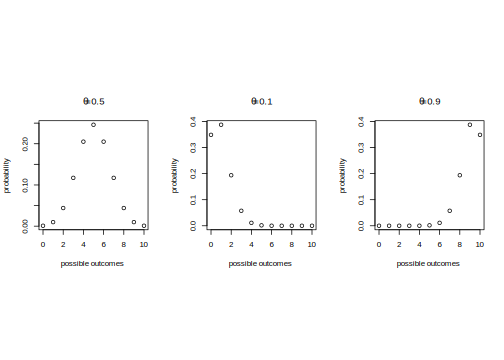
\includegraphics[width=0.3\linewidth]{bookdown_files/figure-latex/binomplot-1} 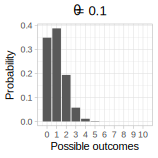
\includegraphics[width=0.3\linewidth]{bookdown_files/figure-latex/binomplot-2} 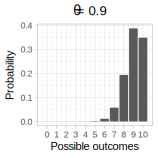
\includegraphics[width=0.3\linewidth]{bookdown_files/figure-latex/binomplot-3} \caption{Probability mass functions of a binomial distribution assuming 10 trials, with 50\%, 10\%, and 90\% probability of success.}\label{fig:binomplot}
\end{figure}

The probability mass function for the binomial is written as follows.

\begin{equation}
\mathit{Binomial}(k|n,\theta) = 
\binom{n}{k} \theta^{k} (1-\theta)^{n-k}
\end{equation}

Here, \(n\) represents the total number of trials, \(k\) the number of successes (this could range from 0 to 10), and \(\theta\) the probability of success. The term \(\binom{n}{k}\), pronounced n-choose-k, represents the number of ways in which one can choose \(k\) successes out of \(n\) trials. For example, 1 success out of 10 can occur in 10 possible ways: the very first trial could be a 1, the secone trial could be a 1, etc.
The term \(\binom{n}{k}\) expands to \(\frac{n!}{k!(n-k)!}\). In R, it is computed using the function \texttt{choose(n,k)}, with \(n\) and \(k\) representing positive integer values.

When we want to express the fact that the data is assumed to be generated from a binomial random variable, we will write \(Y \sim \mathit{Binomial}(n,\theta)\), where \(\sim\) should be read as ``is being generated from''. If the data is generated from a random variable that has some other probability distribution \(f(\theta)\), we will write \(Y\sim f(\theta)\). We are using \(f(\cdot)\) synonymously with \(p(\cdot)\) to represent a probability distribution.

\hypertarget{the-mean-and-variance-of-the-binomial-distribution}{%
\subsection{The mean and variance of the binomial distribution}\label{the-mean-and-variance-of-the-binomial-distribution}}

It is possible to analytically compute the mean (expectation) and variance of the PMF associated with the binomial random variable \(Y\).

The expectation of a discrete random variable \(Y\) with probability mass function f(y), is defined as

\begin{equation}
E[Y] = \sum_y y \cdot f(y)
\end{equation}

As a really simple example, suppose that we toss a fair coin once. The possible outcomes are Tails (represented as 0) and Heads (represented as 1), each with equal probability, 0.5. The expectation is:

\begin{equation}
E[Y] = \sum_y y \cdot f(y) = 0\cdot 0.5 + 1\cdot 0.5 = 0.5 
\end{equation}

The expectation has the interpretation that if we were to do the experiment a large number of times and calculate the sample mean of the observations, in the long run we would approach the value 0.5. Another way to look at the above definition is that the expectation gives us the weighted mean of the possible outcomes, weighted by the respective probabilities of each outcome.

Without getting into the details of how these are derived mathematically (Kerns \protect\hyperlink{ref-kerns2014introduction}{2014}), we just state here that the mean of \(Y\) (the expectation \(E[Y]\)) and variance of \(Y\) (written \(Var(Y)\)) of a binomial distribution with parameter \(\theta\) and \(n\) trials are \(E[Y] = n\theta\) and \(Var(Y) = n\theta (1-\theta)\).

In the binomial example above, \(n\) is a fixed number because we decide on the total number of trials before running the experiment. In the PMF, \(\theta\) is also a fixed value; the only variable in a PMF is \(k\). In real experimental situations we never know the true value of \(\theta\). But \(\theta\) can be estimated from the data. From the observed data, we can compute the estimate of \(\theta\), \(\hat \theta=k/n\). The quantity \(\hat \theta\) is the observed proportion of successes, and is called the \emph{maximum likelihood estimate} of the true (but unknown) parameter \(\theta\). Once we have estimated \(\theta\) in this way, we can also obtain an estimate of the variance by computing \(n\theta (1-\theta)\). These estimates are then used for statistical inference.

What does the term ``maximum likelihood estimate'' mean? The term \emph{likelihood} refers to the binomial distribution function, i.e., the PMF we saw above, \(p(k|n,\theta)\); the difference is that the binomial distribution is seen as a function of \(\theta\), having observed a particular value for \(k\) (i.e., \(k\) is now fixed, along with \(n\)). Recall that the PMF assumes that \(\theta\) and \(n\) are fixed, and \(k\) will vary from 0 to 10 when the experiment is repeated multiple times. The likelihood function is the same function as the PMF, \(p(k|n,\theta)\), but assumes that the data is fixed and only the parameter \(\theta\) varies (from 0 to 1). The likelihood function is written \(\mathcal{L}(\theta| k,n)\).

For example, suppose that we record \(n=10\) trials, and observe \(k=7\) successes. What is the probability of observing \(7\) successes out of \(10\)? We need the binomial distribution to compute this value:

\begin{equation}
\mathcal{L}(\theta|k=7,n=10)=\mathit{Binomial}(k=7,n=10|\theta) = 
\binom{10}{7} \theta^{7} (1-\theta)^{10-7}
\end{equation}

If we now plot the likelihood function for all possible values of \(\theta\) ranging from \(0\) to \(1\), we get the plot shown in Figure \ref{fig:binomlik}.

\begin{figure}
\centering
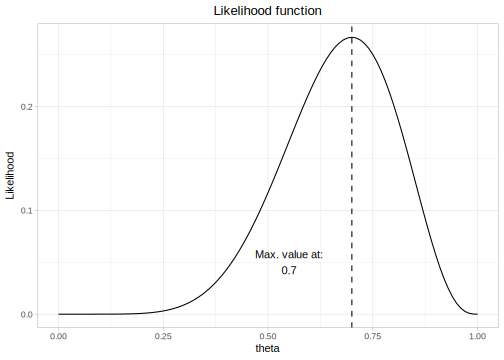
\includegraphics{bookdown_files/figure-latex/binomlik-1.pdf}
\caption{\label{fig:binomlik}The likelihood function for 7 successes out of 10.}
\end{figure}

What is important about this plot is that it shows that, given the data, the maximum point is at the point \(0.7\), which corresponds to the estimated mean using the formula shown above: \(k/n = 7/10\). Thus, the maximum likelihood estimate (MLE) gives us the most likely value that the parameter \(\theta\) has, given the data. In the binomial, the proportion of successes \(k/n\) can be shown to be the maximum likelihood estimate of the parameter \(\theta\).

A crucial point: the ``most likely'' value of the parameter is with respect to the data at hand. The data are used to choose as an estimate of the unknown parameter a value for which the probability (discrete case) or probability density (continuous case) of getting the sample values is a maximum. The MLE from a particular sample of data need not invariably give us an accurate estimate of \(\theta\). For example, if we run our experiment for \(10\) trials and get \(1\) success out of \(10\), the MLE is \(0.10\). We could have just happened to observe only one success out of ten by chance, even if the true \(\theta\) were \(0.7\). If we were to repeatedly run the experiment, in the long run, the MLE computed each time would converge around the true value of the parameter. Figure \ref{fig:lawlargenos} illustrates this point.

\begin{figure}
\centering
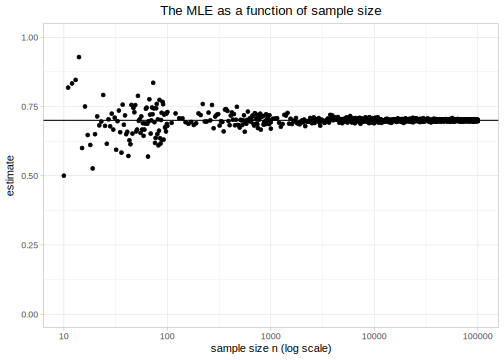
\includegraphics{bookdown_files/figure-latex/lawlargenos-1.pdf}
\caption{\label{fig:lawlargenos}The plot shows the estimate of the mean proportion of successes sampled from a binomial distribution with true probability of success 0.7, with increasing sample sizes. As the sample size increases, the estimate converges to the true value of 0.7.}
\end{figure}

\hypertarget{what-information-does-a-probability-distribution-provide}{%
\subsection{What information does a probability distribution provide?}\label{what-information-does-a-probability-distribution-provide}}

In Bayesian data analysis, we will constantly be asking the question: what information does a probability distribution give us? In particular, we will treat each parameter \(\theta\) as a random variable; this will raise questions like: ``what is the probability that the parameter \(\theta\) lies between two values \(a\) and \(b\)''; and ``what is the range over which we can be 95\% certain that the true value of the parameter lies''? In order to be able to answer questions like these, we need to know what information we can obtain once we have decided on a probability distribution that is assumed to have generated the data, and how to extract this information using R. We therefore discuss the different kinds of information we can obtain from a probability distribution. For now we focus only on the binomial random variable introduced above.

\hypertarget{compute-the-probability-of-a-particular-outcome-discrete-case-only}{%
\subsubsection{Compute the probability of a particular outcome (discrete case only)}\label{compute-the-probability-of-a-particular-outcome-discrete-case-only}}

The binomial distribution shown in Figure \ref{fig:binomplot} already shows the probability of each possible outcome under a different value for \(\theta\). In R, there is a built-in function that allows us to calculate the probability of \(k\) successes out of \(n\), given a particular value of \(k\) (this number constitutes our data), the number of trials \(n\), and given a particular value of \(\theta\); this is the \texttt{dbinom} function. For example, the probability of 5 successes out of 10 when \(\theta\) is 0.5 is:

\begin{Shaded}
\begin{Highlighting}[]
\KeywordTok{dbinom}\NormalTok{(}\DecValTok{5}\NormalTok{, }\DataTypeTok{size =} \DecValTok{10}\NormalTok{, }\DataTypeTok{prob =} \FloatTok{0.5}\NormalTok{)}
\end{Highlighting}
\end{Shaded}

\begin{verbatim}
## [1] 0.246
\end{verbatim}

The probabilities of success when \(\theta\) is 0.1 or 0.9 can be computed by replacing 0.5 above by each of these probabilities. One can just do this by giving \texttt{dbinom} a vector of probabilities:

\begin{Shaded}
\begin{Highlighting}[]
\KeywordTok{dbinom}\NormalTok{(}\DecValTok{5}\NormalTok{, }\DataTypeTok{size =} \DecValTok{10}\NormalTok{, }\DataTypeTok{prob =} \KeywordTok{c}\NormalTok{(}\FloatTok{0.1}\NormalTok{, }\FloatTok{0.9}\NormalTok{))}
\end{Highlighting}
\end{Shaded}

\begin{verbatim}
## [1] 0.00149 0.00149
\end{verbatim}

The probability of a particular outcome like \(k=5\) successes is only computable in the discrete case. In the continuous case, the probability of obtaining a particular point value will always be zero (we discuss this when we turn to continuous probability distributions below).

\hypertarget{compute-the-cumulative-probability-of-k-or-less-more-than-k-successes}{%
\subsubsection{Compute the cumulative probability of k or less (more) than k successes}\label{compute-the-cumulative-probability-of-k-or-less-more-than-k-successes}}

Using the \texttt{dbinom} function, we can compute the cumulative probability of obtaining 1 or less, 2 or less successes etc. This is done through a simple summation procedure:

\begin{Shaded}
\begin{Highlighting}[]
\CommentTok{## the cumulative probability of obtaining}
\CommentTok{## 0, 1, or 2 successes out of 10,}
\CommentTok{## with theta=0.5:}
\KeywordTok{dbinom}\NormalTok{(}\DecValTok{0}\NormalTok{, }\DataTypeTok{size =} \DecValTok{10}\NormalTok{, }\DataTypeTok{prob =} \FloatTok{0.5}\NormalTok{) }\OperatorTok{+}
\StringTok{  }\KeywordTok{dbinom}\NormalTok{(}\DecValTok{1}\NormalTok{, }\DataTypeTok{size =} \DecValTok{10}\NormalTok{, }\DataTypeTok{prob =} \FloatTok{0.5}\NormalTok{) }\OperatorTok{+}
\StringTok{  }\KeywordTok{dbinom}\NormalTok{(}\DecValTok{2}\NormalTok{, }\DataTypeTok{size =} \DecValTok{10}\NormalTok{, }\DataTypeTok{prob =} \FloatTok{0.5}\NormalTok{)}
\end{Highlighting}
\end{Shaded}

\begin{verbatim}
## [1] 0.0547
\end{verbatim}

Mathematically, we could write the above summation as:

\begin{equation}
\sum_{k=0}^2 \binom{n}{k} \theta^{k} (1-\theta)^{n-k} 
\end{equation}

An alternative to the cumbersome addition in the R code above is this more compact statement, which closely mimics the above mathematical expression:

\begin{Shaded}
\begin{Highlighting}[]
\KeywordTok{sum}\NormalTok{(}\KeywordTok{dbinom}\NormalTok{(}\DecValTok{0}\OperatorTok{:}\DecValTok{2}\NormalTok{, }\DataTypeTok{size =} \DecValTok{10}\NormalTok{, }\DataTypeTok{prob =} \FloatTok{0.5}\NormalTok{))}
\end{Highlighting}
\end{Shaded}

\begin{verbatim}
## [1] 0.0547
\end{verbatim}

R has a built-in function called \texttt{pbinom} that does this summation for us. If we want to know the probability of \(2\) or less successes as in the above example, we can write:

\begin{Shaded}
\begin{Highlighting}[]
\KeywordTok{pbinom}\NormalTok{(}\DecValTok{2}\NormalTok{, }\DataTypeTok{size =} \DecValTok{10}\NormalTok{, }\DataTypeTok{prob =} \FloatTok{0.5}\NormalTok{, }\DataTypeTok{lower.tail =} \OtherTok{TRUE}\NormalTok{)}
\end{Highlighting}
\end{Shaded}

\begin{verbatim}
## [1] 0.0547
\end{verbatim}

The specification \texttt{lower.tail\ =\ TRUE} (the default value) ensures that the summation goes from \(2\) to numbers smaller than \(2\) (which lie in the lower tail of the distribution in Figure \ref{fig:binomplot}). If we wanted to know what the probability is of obtaining \(3\) or more successes out of \(10\), we can set \texttt{lower.tail} to \texttt{FALSE}:

\begin{Shaded}
\begin{Highlighting}[]
\KeywordTok{pbinom}\NormalTok{(}\DecValTok{2}\NormalTok{, }\DataTypeTok{size =} \DecValTok{10}\NormalTok{, }\DataTypeTok{prob =} \FloatTok{0.5}\NormalTok{, }\DataTypeTok{lower.tail =} \OtherTok{FALSE}\NormalTok{)}
\end{Highlighting}
\end{Shaded}

\begin{verbatim}
## [1] 0.945
\end{verbatim}

\begin{Shaded}
\begin{Highlighting}[]
\CommentTok{## equivalently:}
\CommentTok{## sum(dbinom(3:10,size = 10, prob = 0.5))}
\end{Highlighting}
\end{Shaded}

The cumulative distribution function or CDF can be plotted by computing the cumulative probabilities for any value \(k\) or less than \(k\), where \(k\) ranges from \(0\) to \(10\) in our running example. The CDF is shown in Figure \ref{fig:binomcdf}.

\begin{figure}
\centering
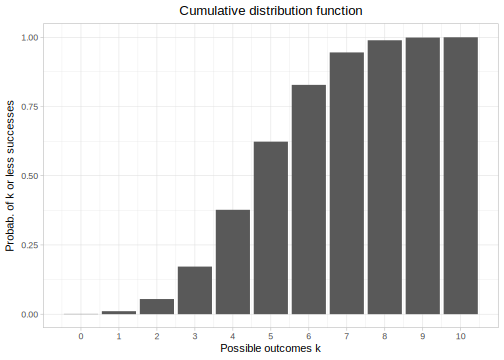
\includegraphics{bookdown_files/figure-latex/binomcdf-1.pdf}
\caption{\label{fig:binomcdf}The cumulative distribution function for a binomial distribution assuming 10 trials, with 50\% probability of success.}
\end{figure}

\hypertarget{compute-the-inverse-of-the-cumulative-distribution-function-the-quantile-function}{%
\subsubsection{Compute the inverse of the cumulative distribution function (the quantile function)}\label{compute-the-inverse-of-the-cumulative-distribution-function-the-quantile-function}}

We can also find out the value of the variable \(k\) (the quantile) such that the probability of obtaining \(k\) or less than \(k\) successes is some specific probability value \(p\). If we switch the x and y axes of Figure \ref{fig:binomcdf}, we obtain another very useful function, the inverse CDF.

The inverse of the CDF (known as the quantile function in R because it returns the quantile, the value \(k\)) is available in R as the function \texttt{qbinom}. The usage is as follows: to find out what the value \(k\) of the outcome is such that the probability of obtaining \(k\) or less successes is \(0.37\), type:

\begin{Shaded}
\begin{Highlighting}[]
\KeywordTok{qbinom}\NormalTok{(}\FloatTok{0.37}\NormalTok{, }\DataTypeTok{size =} \DecValTok{10}\NormalTok{, }\DataTypeTok{prob =} \FloatTok{0.5}\NormalTok{)}
\end{Highlighting}
\end{Shaded}

\begin{verbatim}
## [1] 4
\end{verbatim}

One can visualize the inverse CDF of the binomial as in Figure \ref{fig:inverseCDFbinomial}.

\begin{figure}
\centering
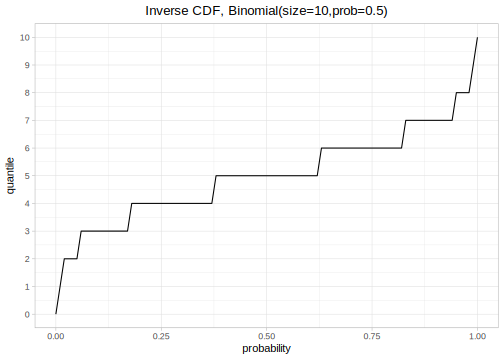
\includegraphics{bookdown_files/figure-latex/inverseCDFbinomial-1.pdf}
\caption{\label{fig:inverseCDFbinomial}The inverse CDF for the binomial(size=10,prob=0.5).}
\end{figure}

\hypertarget{generate-simulated-data-from-a-mathitbinomialntheta-distribution}{%
\subsubsection{\texorpdfstring{Generate simulated data from a \(\mathit{Binomial}(n,\theta)\) distribution}{Generate simulated data from a \textbackslash{}mathit\{Binomial\}(n,\textbackslash{}theta) distribution}}\label{generate-simulated-data-from-a-mathitbinomialntheta-distribution}}

We can generate simulated data from a binomial distribution by specifying the number of trials and the probability of success \(\theta\). In R, we do this as follows:

\begin{Shaded}
\begin{Highlighting}[]
\KeywordTok{rbinom}\NormalTok{(}\DecValTok{1}\NormalTok{, }\DataTypeTok{size =} \DecValTok{10}\NormalTok{, }\DataTypeTok{prob =} \FloatTok{0.5}\NormalTok{)}
\end{Highlighting}
\end{Shaded}

\begin{verbatim}
## [1] 5
\end{verbatim}

The above code generates the number of successes in an experiment with \(10\) trials. Repeatedly run the above code; we will get different numbers of successes each time.

As mentioned earlier, if there is only one trial, then instead of the binomial distribution, we have a Bernoulli distribution. For example, if we have 10 observations from a Bernoulli distribution, where the probability of success if 0.5, we can simulate data as follows using the function \texttt{rbern} from the package \texttt{extraDistr}.

\begin{Shaded}
\begin{Highlighting}[]
\KeywordTok{rbern}\NormalTok{(}\DataTypeTok{n=}\DecValTok{10}\NormalTok{,}\DataTypeTok{prob=}\FloatTok{0.5}\NormalTok{)}
\end{Highlighting}
\end{Shaded}

\begin{verbatim}
##  [1] 0 1 0 1 1 1 0 1 0 0
\end{verbatim}

The above kind of output can also be generated by using the \texttt{rbinom} function: \texttt{rbinom(10,\ size\ =\ 1,\ prob\ =\ 0.5)}.
When the data are generated using the \texttt{rbinom} function in this way, one can calculate the number of successes by just summing up the vector, or computing its mean and multiplying by the number of trials, here \(10\):

\begin{Shaded}
\begin{Highlighting}[]
\NormalTok{(y <-}\StringTok{ }\KeywordTok{rbinom}\NormalTok{(}\DecValTok{10}\NormalTok{, }\DataTypeTok{size =} \DecValTok{1}\NormalTok{, }\DataTypeTok{prob =} \FloatTok{0.5}\NormalTok{))}
\end{Highlighting}
\end{Shaded}

\begin{verbatim}
##  [1] 0 1 0 0 0 0 1 0 1 1
\end{verbatim}

\begin{Shaded}
\begin{Highlighting}[]
\KeywordTok{mean}\NormalTok{(y) }\OperatorTok{*}\StringTok{ }\DecValTok{10}
\end{Highlighting}
\end{Shaded}

\begin{verbatim}
## [1] 4
\end{verbatim}

\begin{Shaded}
\begin{Highlighting}[]
\KeywordTok{sum}\NormalTok{(y)}
\end{Highlighting}
\end{Shaded}

\begin{verbatim}
## [1] 4
\end{verbatim}

\hypertarget{continuous-random-variables-an-example-using-the-normal-distribution}{%
\section{Continuous random variables: An example using the normal distribution}\label{continuous-random-variables-an-example-using-the-normal-distribution}}

We will now revisit the idea of the random variable using a continuous distribution. Imagine that we have a vector of reading time data \(y\) measured in milliseconds and coming from a normal distribution. The normal distribution is defined in terms of two parameters: the \emph{location}, its mean value \(\mu\), which determines its center, and the \emph{scale}, its standard devation, \(\sigma\), which determines how much spread there is around this center point.

The probability density function (PDF) of the normal distribution is defined as follows:

\begin{equation}
\mathit{Normal}(y|\mu,\sigma)=f(y)= \frac{1}{\sqrt{2\pi \sigma^2}} \exp \left(-\frac{(y-\mu)^2}{2\sigma^2} \right)
\end{equation}

Here, \(\mu\) is some true, unknown mean, and \(\sigma^2\) is some true, unknown variance of the normal distribution that the reading times have been sampled from. There is a built-in function in R that computes the above function once we specify the mean \(\mu\) and the standard deviation \(\sigma\) (in R, this parameter is specified in terms of the standard deviation rather than the variance).

Figure \ref{fig:normdistrn} visualizes the normal distribution for particular values of \(\mu\) and \(\sigma\), as a PDF (using \texttt{dnorm}), a CDF (using \texttt{pnorm}), and the inverse CDF (using \texttt{qnorm}). It is clear from the figure that these are three different ways of looking at the same information.

\begin{figure}
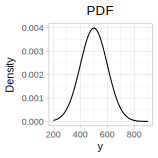
\includegraphics[width=0.3\linewidth]{bookdown_files/figure-latex/normdistrn-1} 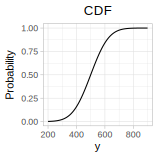
\includegraphics[width=0.3\linewidth]{bookdown_files/figure-latex/normdistrn-2} 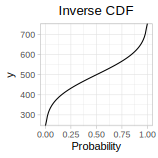
\includegraphics[width=0.3\linewidth]{bookdown_files/figure-latex/normdistrn-3} \caption{The PDF, CDF, and inverse CDF for the $\mathit{Normal}(\mu=500,\sigma=100)$.}\label{fig:normdistrn}
\end{figure}

As in the discrete example, the PDF, CDF, and inverse of the CDF allow us to ask questions like:

\begin{itemize}
\tightlist
\item
  What is the probability of observing values between \(a\) and \(b\) from a normal distribution with mean \(\mu\) and standard deviation \(\sigma\)? Using the above example, we can ask what the probability of observing values between 200 and 700 ms:
\end{itemize}

\begin{Shaded}
\begin{Highlighting}[]
\KeywordTok{pnorm}\NormalTok{(}\DecValTok{700}\NormalTok{, }\DataTypeTok{mean =} \DecValTok{500}\NormalTok{, }\DataTypeTok{sd =} \DecValTok{100}\NormalTok{) }\OperatorTok{-}\StringTok{ }\KeywordTok{pnorm}\NormalTok{(}\DecValTok{200}\NormalTok{, }\DataTypeTok{mean =} \DecValTok{500}\NormalTok{, }\DataTypeTok{sd =} \DecValTok{100}\NormalTok{)}
\end{Highlighting}
\end{Shaded}

\begin{verbatim}
## [1] 0.976
\end{verbatim}

The probability of any point value in a PDF is always \(0\). This is because the probability in a continuous probability distribution is the area under the curve, and the area at any point on the x-axis is always \(0\). The implication here is that it is only meaningful to ask about probabilities between two different point values; e.g., the probability that \(Y\) lies between \(a\) and \(b\), or \(P(a<Y<b)\).

\begin{itemize}
\tightlist
\item
  What is the quantile \(q\) such that the probability of observing that value \(q\) or something less (or more) than it is \(p\)? For example, we can work out the quantile \(q\) such that the probability of observing \(q\) or something less than it is 0.975, in the normal(500,100) distribution. Formally, we would write this as \(P(Y<a)\).
\end{itemize}

\begin{Shaded}
\begin{Highlighting}[]
\KeywordTok{qnorm}\NormalTok{(}\FloatTok{0.975}\NormalTok{, }\DataTypeTok{mean =} \DecValTok{500}\NormalTok{, }\DataTypeTok{sd =} \DecValTok{100}\NormalTok{)}
\end{Highlighting}
\end{Shaded}

\begin{verbatim}
## [1] 696
\end{verbatim}

The above output says that the quantile value \(q\) such that \(Prob(X<q)=0.975\) is \(695\).

\begin{itemize}
\tightlist
\item
  Generate simulated data. Given a vector of \(n\) independent and identically distributed data \(y\), i.e., given that each data point is being generated independently from \(Y \sim \mathit{Normal}(\mu,\sigma)\) for some values of the parameters, the sample mean and standard deviation\footnote{R will compute the standard deviation by dividing by \(n-1\), not \(n\); this is because dividing by \(n\) gives a biased estimate. This is not an important detail for our purposes, and in any case for large \(n\) it doesn't really matter whether one divides by \(n\) or \(n-1\).} are:
\end{itemize}

\begin{equation}
\bar{y} =  \frac{\sum_{i=1}^n y_i}{n} 
\end{equation}

\begin{equation}
sd(y) = \sqrt{\frac{\sum_{i=1}^n (y_i-
\bar{y})^2}{n}}
\end{equation}

For example, we can generate \(10\) data points using the \texttt{rnorm} function, and then use the simulated data to compute the mean and standard deviation:

\begin{Shaded}
\begin{Highlighting}[]
\NormalTok{y <-}\StringTok{ }\KeywordTok{rnorm}\NormalTok{(}\DecValTok{10}\NormalTok{, }\DataTypeTok{mean =} \DecValTok{500}\NormalTok{, }\DataTypeTok{sd =} \DecValTok{100}\NormalTok{)}
\KeywordTok{mean}\NormalTok{(y)}
\end{Highlighting}
\end{Shaded}

\begin{verbatim}
## [1] 527
\end{verbatim}

\begin{Shaded}
\begin{Highlighting}[]
\KeywordTok{sd}\NormalTok{(y)}
\end{Highlighting}
\end{Shaded}

\begin{verbatim}
## [1] 97
\end{verbatim}

Again, the sample mean and sample standard deviation computed from a particular (simulated or real) data set need not necessarily be close to the true values of the respective parameters. Especially when sample size is small, one can end up with missestimates of the mean and sd.

Incidentally, simulated data can be used to generate all kinds of statistics. For example, we can compute the lower and upper bounds of a 95\% confidence interval from simulated data as follows:

\begin{Shaded}
\begin{Highlighting}[]
\KeywordTok{quantile}\NormalTok{(y, }\DataTypeTok{probs =} \KeywordTok{c}\NormalTok{(}\FloatTok{0.025}\NormalTok{, }\FloatTok{0.975}\NormalTok{))}
\end{Highlighting}
\end{Shaded}

\begin{verbatim}
##  2.5% 97.5% 
##   373   639
\end{verbatim}

Later on, we will be using samples to produce summary statistics like the ones shown above.

\hypertarget{an-important-distinction-probability-vs.density-in-a-continuous-random-variable}{%
\subsection{An important distinction: probability vs.~density in a continuous random variable}\label{an-important-distinction-probability-vs.density-in-a-continuous-random-variable}}

In continuous distributions like the normal discussed above, it is important to understand that the probability density function or PDF, \(p(y| \mu, \sigma)\) defines a mapping from the \(y\) values (the possible values that the data can have) to a quantity called the density of each possible value. We can see this function in action when we use \texttt{dnorm} to compute, say, the density value corresponding to \(y=1\) in the \(\mathit{Normal}(\mu=0,\sigma=1)\) distribution.

\begin{Shaded}
\begin{Highlighting}[]
\CommentTok{## density:}
\KeywordTok{dnorm}\NormalTok{(}\DecValTok{1}\NormalTok{, }\DataTypeTok{mean =} \DecValTok{0}\NormalTok{, }\DataTypeTok{sd =} \DecValTok{1}\NormalTok{)}
\end{Highlighting}
\end{Shaded}

\begin{verbatim}
## [1] 0.242
\end{verbatim}

The quantity above is \emph{not} the probability of observing 1 in this distribution. As mentioned earlier, probability in a continuous distribution is the area under the curve, and this area will always be zero at any point value. If we want to know the probability of obtaining values between an upper and lower bound \(b\) and \(a\), i.e., \(P(a<Y<b)\) where these are two distinct values, we must use the cumulative distribution function or CDF: in R, for the normal distribution, this is the \texttt{pnorm} function. For example, the probability of observing a value between +2 and -2 in a normal distribution with mean 0 and standard deviation 1 is:

\begin{Shaded}
\begin{Highlighting}[]
\KeywordTok{pnorm}\NormalTok{(}\DecValTok{2}\NormalTok{, }\DataTypeTok{mean =} \DecValTok{0}\NormalTok{, }\DataTypeTok{sd =} \DecValTok{1}\NormalTok{) }\OperatorTok{-}\StringTok{ }\KeywordTok{pnorm}\NormalTok{(}\OperatorTok{-}\DecValTok{2}\NormalTok{, }\DataTypeTok{mean =} \DecValTok{0}\NormalTok{, }\DataTypeTok{sd =} \DecValTok{1}\NormalTok{)}
\end{Highlighting}
\end{Shaded}

\begin{verbatim}
## [1] 0.954
\end{verbatim}

The situation is different in discrete random variables. These have a probability mass function (PMF) associated with them---the binomial distribution that we saw earlier is an example. There, the PMF maps the possible \(y\) values to the probabilities of those values occurring. That is why, in the binomial distribution, the probability of observing exactly 2 successes when sampling from a \(\mathit{Binomial}(n=10,\theta=0.5)\) can be computed using either \texttt{dbinom} or \texttt{pbinom}:

\begin{Shaded}
\begin{Highlighting}[]
\KeywordTok{dbinom}\NormalTok{(}\DecValTok{2}\NormalTok{, }\DataTypeTok{size =} \DecValTok{10}\NormalTok{, }\DataTypeTok{prob =} \FloatTok{0.5}\NormalTok{)}
\end{Highlighting}
\end{Shaded}

\begin{verbatim}
## [1] 0.0439
\end{verbatim}

\begin{Shaded}
\begin{Highlighting}[]
\KeywordTok{pbinom}\NormalTok{(}\DecValTok{2}\NormalTok{, }\DataTypeTok{size =} \DecValTok{10}\NormalTok{, }\DataTypeTok{prob =} \FloatTok{0.5}\NormalTok{) }\OperatorTok{-}\StringTok{ }\KeywordTok{pbinom}\NormalTok{(}\DecValTok{1}\NormalTok{, }\DataTypeTok{size =} \DecValTok{10}\NormalTok{, }\DataTypeTok{prob =} \FloatTok{0.5}\NormalTok{)}
\end{Highlighting}
\end{Shaded}

\begin{verbatim}
## [1] 0.0439
\end{verbatim}

In the second line of code above, we are computing the cumulative probability of observing two or less successes, minus the probability of observing one or less successes. This gives us the probability of observing exactly two successes. The \texttt{dbinom} gives us this same information.

\hypertarget{truncating-a-normal-distribution}{%
\subsection{Truncating a normal distribution}\label{truncating-a-normal-distribution}}

In the above discussion, the support for the normal distribution ranges from minus infinity to plus infinity. One can define PDFs with a more limited support; an example would be a normal distribution whose PDF \(f(x)\) is such that the lower bound is truncated at \(0\) to allow only positive values. In such a case, the area under the range minus infinity to zero (\(\int_{-\infty}^0 f(x) \, dx\)) will be \(0\) because the range lies outside the support of the truncated normal distribution. Also, if one truncates a probability density function like the standard normal (\(\mathit{Normal}(0,1)\)) at \(0\), in order to make the area between zero and plus infinity sum up to \(1\), we would have to multiply the truncated distribution f(x) by some factor \(k\) such that the following integral sums to \(1\):

\begin{equation}
k \int_{0}^{\infty} f(x)\, dx = 1
\label{eq:factork}
\end{equation}

Clearly, this factor is \(k = \frac{1}{\int_{0}^{\infty} f(x)\, dx}\). For the standard normal, this integral is easy to compute; we just calculate the complement of the cumulative distribution (CCDF):

\begin{Shaded}
\begin{Highlighting}[]
\KeywordTok{pnorm}\NormalTok{(}\DecValTok{0}\NormalTok{, }\DataTypeTok{mean =} \DecValTok{0}\NormalTok{, }\DataTypeTok{sd =} \DecValTok{1}\NormalTok{, }\DataTypeTok{lower.tail =} \OtherTok{FALSE}\NormalTok{)}
\end{Highlighting}
\end{Shaded}

\begin{verbatim}
## [1] 0.5
\end{verbatim}

\begin{Shaded}
\begin{Highlighting}[]
\CommentTok{## alternatively:}
\DecValTok{1} \OperatorTok{-}\StringTok{ }\KeywordTok{pnorm}\NormalTok{(}\DecValTok{0}\NormalTok{, }\DataTypeTok{mean =} \DecValTok{0}\NormalTok{, }\DataTypeTok{sd =} \DecValTok{1}\NormalTok{, }\DataTypeTok{lower.tail =} \OtherTok{TRUE}\NormalTok{)}
\end{Highlighting}
\end{Shaded}

\begin{verbatim}
## [1] 0.5
\end{verbatim}

Also, if we had truncated the distribution at 0 to the right instead of the left (allowing only negative values), we would have to find the factor \(k\) in the same way as above, except that we would have to find \(k\) such that:

\begin{equation}
k \int_{-\infty}^{0} f(x)\, dx = 1
\end{equation}

For the standard normal case, in R, this factor would require us to use the CDF:

\begin{Shaded}
\begin{Highlighting}[]
\KeywordTok{pnorm}\NormalTok{(}\DecValTok{0}\NormalTok{, }\DataTypeTok{mean =} \DecValTok{0}\NormalTok{, }\DataTypeTok{sd =} \DecValTok{1}\NormalTok{, }\DataTypeTok{lower.tail =} \OtherTok{TRUE}\NormalTok{)}
\end{Highlighting}
\end{Shaded}

\begin{verbatim}
## [1] 0.5
\end{verbatim}

Later in this book, we will be using such truncated distributions when doing Bayesian modeling, and when we use them, we will want to multiply the truncated distribution by the factor \(k\) to ensure that it is still a proper PDF that sums to \(1\). Truncated normal distributions will be discussed in more detail in Box \ref{thm:truncation}.

\hypertarget{bivariate-and-multivariate-distributions}{%
\section{Bivariate and multivariate distributions}\label{bivariate-and-multivariate-distributions}}

So far, we have only discussed univariate distributions. It is also possible to specify distributions with two or more dimensions.

\hypertarget{example-1-discrete-bivariate-distributions}{%
\subsection{Example 1: Discrete bivariate distributions}\label{example-1-discrete-bivariate-distributions}}

Starting with the discrete case, consider the discrete bivariate distribution shown below. These are data from an experiment where, inter alia, in each trial a Likert acceptability rating and a question-response accuracy were recorded (the data are from a study by Laurinavichyute (\protect\hyperlink{ref-AnnaLphd}{2020}), used with permission here). Load the data by loading the R package \texttt{bcogsci}.

\begin{Shaded}
\begin{Highlighting}[]
\KeywordTok{data}\NormalTok{(}\StringTok{"df_discreteagrmt"}\NormalTok{)}
\end{Highlighting}
\end{Shaded}

Figure \ref{fig:bivardiscrete} shows the \emph{joint probability mass function} of two random variables X and Y. The random variable X consists of 7 possible values (this is the 1-7 Likert response scale), and the random variable Y is question-response accuracy, with 0 representing an incorrect response, and 1 representing a correct response.

\begin{figure}
\centering
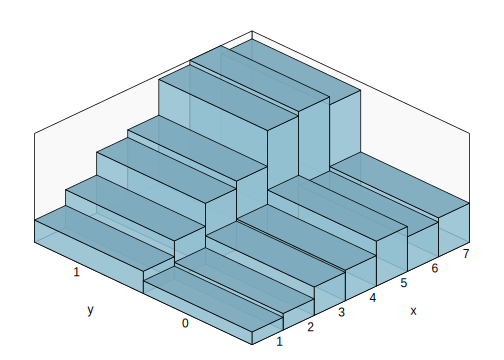
\includegraphics{bookdown_files/figure-latex/bivardiscrete-1.pdf}
\caption{\label{fig:bivardiscrete}Example of a discrete bivariate distribution. In these data, in every trial, two pieces of information were collected: Likert responses and yes-no question responses. The random variable X represents Likert scale responses on a scale of 1-7. and the random variable Y represents 0, 1 (incorrect, correct) responses to comprehension questions.}
\end{figure}

One can also display Figure \ref{fig:bivardiscrete} as a table; see Table \ref{tab:discbivariatetabular}.

\begin{table}

\caption{\label{tab:discbivariatetabular}The joint PMF for two random variables X and Y.}
\centering
\begin{tabular}[t]{lrrrrrrr}
\toprule
  & x=1 & x=2 & x=3 & x=4 & x=5 & x=6 & x=7\\
\midrule
y=0 & 0.018 & 0.023 & 0.040 & 0.043 & 0.063 & 0.049 & 0.055\\
y=1 & 0.031 & 0.053 & 0.086 & 0.096 & 0.147 & 0.153 & 0.142\\
\bottomrule
\end{tabular}
\end{table}

For each possible pair of values of X and Y, we have a joint probability \(p_{X,Y}(x,y)\). Given such a bivariate distribution, there are two useful quantities we can compute: the \emph{marginal} distributions (\(p_{X}\) and \(p_Y\)), and the \emph{conditional} distributions (\(p_{X|Y}\) and \(p_{Y|X}\)).\\
Table \ref{tab:discbivariatetabular} shows the joint probability mass function \(p_{X,Y}(x,y)\).

\hypertarget{sec:marginalizing}{%
\subsubsection{Marginal distributions}\label{sec:marginalizing}}

The marginal distribution \(p_Y\) is defined as follows. \(S_{X}\) is the support of X, i.e., all the possible values of X.

\begin{equation}
p_{Y}(y)=\sum_{x\in S_{X}}p_{X,Y}(x,y).\label{eq-marginal-pmf}
\end{equation}

Similarly, the marginal distribution \(p_X\) is defined as:

\begin{equation}
p_{X}(x)=\sum_{y\in S_{Y}}p_{X,Y}(x,y).\label{eq-marginal-pmf2}
\end{equation}

\(p_Y\) is computed, by summing up the rows; and \(p_X\) by summing up the columns. We can see why this is called the marginal distribution; the result appears in the margins of the table.

\begin{Shaded}
\begin{Highlighting}[]
\CommentTok{# P(Y)}
\NormalTok{(PY <-}\StringTok{ }\KeywordTok{rowSums}\NormalTok{(probs))}
\end{Highlighting}
\end{Shaded}

\begin{verbatim}
##   y=0   y=1 
## 0.291 0.709
\end{verbatim}

\begin{Shaded}
\begin{Highlighting}[]
\KeywordTok{sum}\NormalTok{(PY) }\CommentTok{## sums to 1}
\end{Highlighting}
\end{Shaded}

\begin{verbatim}
## [1] 1
\end{verbatim}

\begin{Shaded}
\begin{Highlighting}[]
\CommentTok{# P(X)}
\NormalTok{(PX <-}\StringTok{ }\KeywordTok{colSums}\NormalTok{(probs))}
\end{Highlighting}
\end{Shaded}

\begin{verbatim}
##    x=1    x=2    x=3    x=4    x=5    x=6    x=7 
## 0.0491 0.0766 0.1257 0.1394 0.2102 0.2020 0.1969
\end{verbatim}

\begin{Shaded}
\begin{Highlighting}[]
\KeywordTok{sum}\NormalTok{(PX) }\CommentTok{## sums to 1}
\end{Highlighting}
\end{Shaded}

\begin{verbatim}
## [1] 1
\end{verbatim}

The marginal probabilities sum to 1, as they should. Table \ref{tab:discbivariatetabularmarginal} shows the marginal probabilities.

\begin{table}

\caption{\label{tab:discbivariatetabularmarginal}The joint PMF for two random variables X and Y, along with the marginal distributions of X and Y.}
\centering
\begin{tabular}[t]{lllllllll}
\toprule
  & x=1 & x=2 & x=3 & x=4 & x=5 & x=6 & x=7 & P(Y)\\
\midrule
y=0 & 0.018 & 0.023 & 0.04 & 0.043 & 0.063 & 0.049 & 0.055 & 0.291\\
y=1 & 0.031 & 0.053 & 0.086 & 0.096 & 0.147 & 0.153 & 0.142 & 0.709\\
P(X) & 0.049 & 0.077 & 0.126 & 0.139 & 0.21 & 0.202 & 0.197 & \\
\bottomrule
\end{tabular}
\end{table}

To compute the marginal distribution of X, one is summing over all the Ys; and to compute the marginal distribution of Y, one sums over all the X's. We say that we are \emph{marginalizing out} the random variable that we are summing over. One can also visualize the two marginal distributions using barplots (Figure \ref{fig:marginalbarplot}).

\begin{figure}
\centering
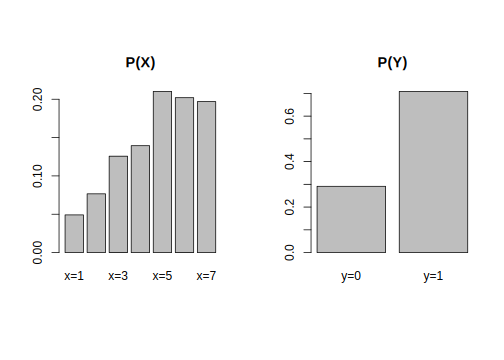
\includegraphics{bookdown_files/figure-latex/marginalbarplot-1.pdf}
\caption{\label{fig:marginalbarplot}The marginal distributions of the random variables X and Y, presented as barplots.}
\end{figure}

\hypertarget{conditional-distributions}{%
\subsubsection{Conditional distributions}\label{conditional-distributions}}

For computing conditional distributions, recall that conditional probability is defined as:

\begin{equation}
p_{X\mid Y}(x\mid y) = \frac{p_{X,Y}(x,y)}{p_Y(y)}  
\end{equation}

and

\begin{equation}
p_{Y\mid X}(y\mid x) = \frac{p_{X,Y}(x,y)}{p_X(x)}  
\end{equation}

The conditional distribution of a random variable \(X\) given that \(Y=y\), where \(y\) is some specific (fixed) value, is:

\begin{equation}
p_{X\mid Y} (x\mid y) = \frac{p_{X,Y}(x,y)}{p_Y(y)} \quad \hbox{provided } p_Y(y)=P(Y=y)>0
\end{equation}

As an example, let's consider how \(p_{X\mid Y}\) would be computed.
The possible values of \(y\) are \(0,1\), and so we have to find the conditional distribution (defined above) for each of these values. I.e., we have to find \(p_{X\mid Y}(x\mid y=0)\), and \(p_{X\mid Y}(x\mid y=1)\).

Let's do the calculation for \(p_{X\mid Y}(x\mid y=0)\).

\begin{equation}
\begin{split}
p_{X\mid Y} (1\mid 0) =& \frac{p_{X,Y}(1,0)}{p_Y(0)}\\
    =&  \frac{0.018}{0.291}\\
    =& 0.062
\end{split} 
\end{equation}

This conditional probability value will occupy the cell X=1, Y=0 in Table \ref{tab:discbivariatetabularconditional} summarizing the conditional probability distribution \(p_{X|Y}\). In this way, one can fill in the entire table, which will then represent the conditional distributions \(p_{X|Y=0}\) and \(p_{X|Y=1}\). The reader may want to take a few minutes to complete Table \ref{tab:discbivariatetabularconditional}.

\begin{table}

\caption{\label{tab:discbivariatetabularconditional}A table for listing conditional distributions of X given Y.}
\centering
\begin{tabular}[t]{llllllll}
\toprule
  & x=1 & x=2 & x=3 & x=4 & x=5 & x=6 & x=7\\
\midrule
p\_X|Y(x|y=0) & 0.062 &  &  &  &  &  & \\
p\_X|Y(x|y=1) &  &  &  &  &  &  & \\
\bottomrule
\end{tabular}
\end{table}

Similarly, one can construct a table that shows \(p_{Y|X}\).

\hypertarget{covariance-and-correlation}{%
\subsubsection{Covariance and correlation}\label{covariance-and-correlation}}

Here, we briefly define the covariance and correlation of two discrete random variables. For detailed examples and discussion, see the references at the end of the chapter.

The covariance of two (discrete) random variables \(X\) and \(Y\) is defined as follows. \(E[\cdot]\) refers to the expectation of a random variable.

\begin{equation}
Cov(X,Y) = E[(X - E[X])(Y-E[Y])
\end{equation}

It is possible to show that this is equivalent to:

\begin{equation}
Cov(X,Y) = E[XY] - E[X]E[Y]
\end{equation}

The expectation E{[}XY{]} is defined to be:

\begin{equation}
E[XY]=\sum_x \sum_y xy f_{X,Y}(x,y)
\end{equation}

If the standard deviations of the two random variables is \(\sigma_X\) and \(\sigma_Y\), the correlation between the two random variables, \(\rho_{XY}\), is defined as:

\begin{equation}
\rho_{XY} = \frac{Cov(X,Y)}{\sigma_X\sigma_Y}
\end{equation}

\hypertarget{sec:contbivar}{%
\subsection{Example 2: Continuous bivariate distributions}\label{sec:contbivar}}

Consider now the continuous bivariate case; this time, we will use simulated data. Consider two normal random variables \(X\) and \(Y\), each of which coming from, for example, a \(\mathit{Normal}(0,1)\) distribution, with some correlation \(\rho\) between the two random variables.

A bivariate distribution for two random variables \(X\) and \(Y\), each of which comes from a normal distribution, is expressed in terms of the means and standard deviations of each of the two distributions, and the correlation \(\rho_{XY}\) between them. We assume here that the mean of both random variables is 0.
The standard deviations and correlation are expressed in a special form of a \(2\times 2\) matrix called a variance-covariance matrix \(\Sigma\). If \(\rho_{XY}\) is the correlation between the two random variables, and \(\sigma _{X}\) and \(\sigma _{Y}\) the respective standard deviations, the variance-covariance matrix is written as:

\begin{equation}\label{eq:covmatfoundations}
\Sigma
=
\begin{pmatrix}
\sigma _{X}^2  & \rho_{XY}\sigma _{X}\sigma _{Y}\\
\rho_{XY}\sigma _{X}\sigma _{Y}    & \sigma _{Y}^2\\
\end{pmatrix}
\end{equation}

The off-diagonals of this matrix contain the covariance between \(X\) and \(Y\).

One occasionally encounters a ``singularity'' warning when fitting hierarchical models with the package \texttt{lme4}. This warning signals the fact that a variance-covariance matrix involved in the model is not invertible. For more details on what this means, see Fieller (\protect\hyperlink{ref-fieller}{2016}).

The joint distribution of \(X\) and \(Y\) is defined as follows:

\begin{equation}\label{eq:jointpriordistfoundations}
\begin{pmatrix}
  X \\ 
  Y \\
\end{pmatrix}
\sim 
\mathcal{N}_2 \left(
\begin{pmatrix}
  0 \\
  0 \\
\end{pmatrix},
\Sigma
\right)
\end{equation}

The joint PDF is written with reference to the two variables \(f_{X,Y}(x,y)\). It has the property that the area under the curve sums to 1. Formally, we would write this as a double integral: we are summing up the volume under the curve for both \(X\) and \(Y\) (hence the two integrals).

\begin{equation}
\iint_{S_{X,Y}} f_{X,Y}(x,y)\, dx dy = 1
\end{equation}

Here, the terms \(dx\) and \(dy\) express the fact that we are summing the area under the curve along the \(X\) axis and the \(Y\) axis.

The joint CDF would be written as follows. The equation below gives us the probability of observing a value like \((u,v)\) or some value smaller than that (i.e., some \((u',v')\), such that \(u'<u\) and \(v'<v\).

\begin{equation}
\begin{split}
F_{X,Y}(u,v) =& P(X<u,Y<v)\\
             =& \int_{-\infty}^u \int_{-\infty}^v f_{X,Y}(x,y)\, dy dx \hbox{ for } (x,y)\in \mathbb{R}^2\\
\end{split}
\end{equation}

Just as in the discrete case, the marginal distributions can be derived by marginalizing out the other random variable:

\begin{equation}
f_X(x) = \int_{S_Y} f_{X,Y}(x,y)\, dy \quad f_Y(y) = \int_{S_X} f_{X,Y}(x,y)\, dx
\end{equation}

Here, \(S_X\) and \(S_Y\) are the respective supports.

Here, the integral sign \(\int\) is the continuous equivalent of the summation sign \(\sum\) in the discrete case. Luckily, we will never have to compute such integrals ourselves; but it is important to appreciate how a marginal distribution arises from a bivariate distribution---by integrating out or marginalizing out the other random variable.

A visualization will help. The figures below shows a bivariate distribution with zero correlation (Figure \ref{fig:zerocor}), a negative (Figure \ref{fig:negcor}) and a positive correlation (Figure \ref{fig:poscor}).

\begin{figure}
\centering
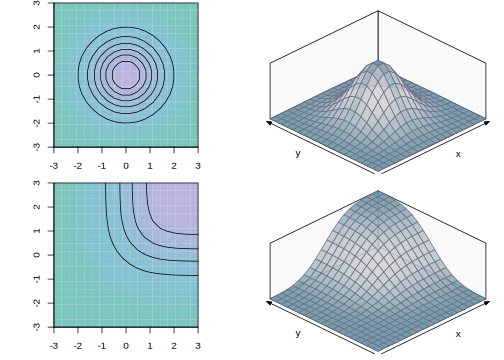
\includegraphics{bookdown_files/figure-latex/zerocor-1.pdf}
\caption{\label{fig:zerocor}A bivariate normal distribution with zero correlation. Shown are four plots: the top-right plot shows the three-dimensional bivariate density, the top-left plot the contour plot of the distribution (seen from above). The lower plots show the cumulative distribution function from two views, as a three-dimensional plot and as a contour plot.}
\end{figure}

\begin{figure}
\centering
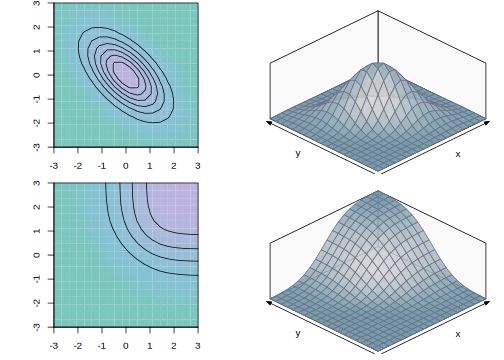
\includegraphics{bookdown_files/figure-latex/negcor-1.pdf}
\caption{\label{fig:negcor}A bivariate normal distribution with a negative correlation of -0.6. Shown are four plots: the top-right plot shows the three-dimensional bivariate density, the top-left plot the contour plot of the distribution (seen from above). The lower plots show the cumulative distribution function from two views, as a three-dimensional plot and as a contour plot.}
\end{figure}

\begin{figure}
\centering
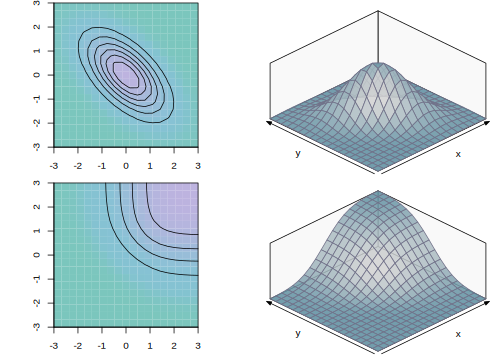
\includegraphics{bookdown_files/figure-latex/poscor-1.pdf}
\caption{\label{fig:poscor}A bivariate normal distribution with a positive correlation of 0.6. Shown are four plots: the top-right plot shows the three-dimensional bivariate density, the top-left plot the contour plot of the distribution (seen from above). The lower plots show the cumulative distribution function from two views, as a three-dimensional plot and as a contour plot.}
\end{figure}

In this book, we will make use of such multivariate distributions a lot, and it will soon become important to know how to generate simulated bivariate or multivariate data that is correlated. So let's look at that next.

\hypertarget{sec:generatebivariatedata}{%
\subsection{Generate simulated bivariate (multivariate) data}\label{sec:generatebivariatedata}}

Suppose we want to generate 100 pairs of correlated data, with correlation \(\rho=0.6\). The two random variables have mean 0, and standard deviations 5 and 10 respectively.

Here is how we would generate such data. First, define a variance-covariance matrix; then, use the multivariate analog of the \texttt{rnorm} function, \texttt{mvrnorm}, from the \texttt{MASS} package to generate \(100\) data-points.

\begin{Shaded}
\begin{Highlighting}[]
\CommentTok{## define a variance-covariance matrix:}
\NormalTok{Sigma <-}\StringTok{ }\KeywordTok{matrix}\NormalTok{(}\KeywordTok{c}\NormalTok{(}\DecValTok{5}\OperatorTok{^}\DecValTok{2}\NormalTok{, }\DecValTok{5} \OperatorTok{*}\StringTok{ }\DecValTok{10} \OperatorTok{*}\StringTok{ }\FloatTok{.6}\NormalTok{, }\DecValTok{5} \OperatorTok{*}\StringTok{ }\DecValTok{10} \OperatorTok{*}\StringTok{ }\FloatTok{.6}\NormalTok{, }\DecValTok{10}\OperatorTok{^}\DecValTok{2}\NormalTok{),}
  \DataTypeTok{byrow =} \OtherTok{FALSE}\NormalTok{, }\DataTypeTok{ncol =} \DecValTok{2}
\NormalTok{)}
\CommentTok{## generate data:}
\NormalTok{u <-}\StringTok{ }\KeywordTok{mvrnorm}\NormalTok{(}
  \DataTypeTok{n =} \DecValTok{100}\NormalTok{,}
  \DataTypeTok{mu =} \KeywordTok{c}\NormalTok{(}\DecValTok{0}\NormalTok{, }\DecValTok{0}\NormalTok{),}
  \DataTypeTok{Sigma =}\NormalTok{ Sigma}
\NormalTok{)}
\KeywordTok{head}\NormalTok{(u, }\DataTypeTok{n =} \DecValTok{3}\NormalTok{)}
\end{Highlighting}
\end{Shaded}

\begin{verbatim}
##       [,1]  [,2]
## [1,] -1.87 -6.50
## [2,] -9.70 -5.33
## [3,]  9.82 13.71
\end{verbatim}

Figure \ref{fig:poscordata} confirms that the simulated data are positively correlated.

\begin{figure}
\centering
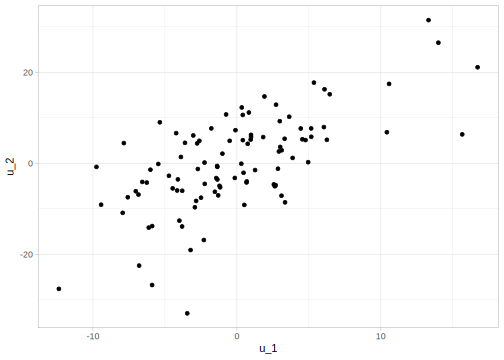
\includegraphics{bookdown_files/figure-latex/poscordata-1.pdf}
\caption{\label{fig:poscordata}The relationship between two positively correlated random variables, generated by simulating data using the R function mvrnorm from the MASS library.}
\end{figure}

One final useful fact about the variance-covariance matrix---one that we will need later---is that it can be decomposed into the component standard deviations and an underlying correlation matrix. For example, consider the matrix above:

\begin{Shaded}
\begin{Highlighting}[]
\NormalTok{Sigma}
\end{Highlighting}
\end{Shaded}

\begin{verbatim}
##      [,1] [,2]
## [1,]   25   30
## [2,]   30  100
\end{verbatim}

One can decompose the matrix as follows. The matrix can be seen as the product of a diagonal matrix of the standard deviations and the correlation matrix:

\begin{Shaded}
\begin{Highlighting}[]
\CommentTok{## sds:}
\NormalTok{(sds <-}\StringTok{ }\KeywordTok{c}\NormalTok{(}\DecValTok{5}\NormalTok{, }\DecValTok{10}\NormalTok{))}
\end{Highlighting}
\end{Shaded}

\begin{verbatim}
## [1]  5 10
\end{verbatim}

\begin{Shaded}
\begin{Highlighting}[]
\CommentTok{## diagonal matrix:}
\NormalTok{(sd_diag <-}\StringTok{ }\KeywordTok{diag}\NormalTok{(sds))}
\end{Highlighting}
\end{Shaded}

\begin{verbatim}
##      [,1] [,2]
## [1,]    5    0
## [2,]    0   10
\end{verbatim}

\begin{Shaded}
\begin{Highlighting}[]
\CommentTok{## correlation matrix:}
\NormalTok{(corrmatrix <-}\StringTok{ }\KeywordTok{matrix}\NormalTok{(}\KeywordTok{c}\NormalTok{(}\DecValTok{1}\NormalTok{, }\FloatTok{0.6}\NormalTok{, }\FloatTok{0.6}\NormalTok{, }\DecValTok{1}\NormalTok{), }\DataTypeTok{ncol =} \DecValTok{2}\NormalTok{))}
\end{Highlighting}
\end{Shaded}

\begin{verbatim}
##      [,1] [,2]
## [1,]  1.0  0.6
## [2,]  0.6  1.0
\end{verbatim}

Given these two matrices, one can reassemble the variance-covariance matrix:\footnote{There is a built-in convenience function, \texttt{sdcor2cov} in the \texttt{SIN} package that does this calculation, taking the vector of standard deviations (not the diagonal matrix) and the correlation matrix to yield the variance-covariance matrix: \texttt{sdcor2cov(stddev\ =\ sds,\ corr\ =\ corrmatrix)}.}

\begin{Shaded}
\begin{Highlighting}[]
\NormalTok{sd_diag }\OperatorTok\StringTok{ }\NormalTok{corrmatrix }\OperatorTok\StringTok{ }\NormalTok{sd_diag}
\end{Highlighting}
\end{Shaded}

\begin{verbatim}
##      [,1] [,2]
## [1,]   25   30
## [2,]   30  100
\end{verbatim}

\hypertarget{sec:marginal}{%
\section{An important concept: The marginal likelihood (integrating out a parameter)}\label{sec:marginal}}

Here, we introduce a concept that will turn up many times in this book. The concept we unpack here is called ``integrating out a parameter''. We will need this when we encounter Bayes' rule in the next chapter, and when we use Bayes factors later in the book (chapter \ref{ch:bf}).

Integrating out a parameter refers to the following situation. Suppose we have a binomial random variable \(Y\) with PMF \(p(Y)\). Suppose also that this PMF is defined in terms of parameter \(\theta\) that can have only three possible values, \(0.1, 0.5, 0.9\), each with equal probability. In other words, the probability that \(\theta\) is \(0.1, 0.5,\) or \(0.9\) is 1/3 each.

We stick with our earlier example of \(n=10\) trials and \(k=7\) successes.
The likelihood function then is

\begin{equation}
p(k=7,n=10|\theta) = \binom{10}{7} \theta^ (1-\theta)^{3}
\end{equation}

There is a related concept of marginal likelihood, which we can write here as \(p(k=7,n=10)\). Marginal likelihood is the likelihood computed by ``marginalizing'' out the parameter \(\theta\): for each possible value that the parameter \(\theta\) can have, we compute the likelihood at that value and multiply that likelihood with the probability/density of that \(\theta\) value occurring. Then we sum up each of the products computed in this way. Mathematically, this means that we carry out the following operation.

In our example, there are three possible values of \(\theta\),
call them \(\theta_1=0.1\), \(\theta_2=0.5\), and \(\theta_3=0.9\). Each has probability \(1/3\); so \(p(\theta_1)=p(\theta_2)=p(\theta_3)=1/3\). Given this information, we can compute the marginal likelihood as follows:

\begin{equation}
\begin{split}
p(k=7,n=10) =& \binom{10}{7} \theta_1^7 (1-\theta_1)^{3} \times p(\theta_1) \\
            +& \binom{10}{7} \theta_2^7 (1-\theta_2)^{3}\times p(\theta_2) \\
            +& \binom{10}{7} \theta_3^7 (1-\theta_3)^{3}\times p(\theta_3)
\end{split}
\end{equation}

Writing the \(\theta\) values and their probabilities, we get:

\begin{equation}
\begin{split}
p(k=7,n=10) =& \binom{10}{7} 0.1^7 (1-0.1)^{3} \times \frac{1}{3} \\
            +& \binom{10}{7} 0.5^7 (1-0.5)^{3}\times \frac{1}{3} \\
            +& \binom{10}{7} 0.9^7 (1-0.9)^{3}\times \frac{1}{3}
\end{split}
\end{equation}

\begin{equation}
\begin{split}
p(k=7,n=10) =& \frac{1}{3} [\binom{10}{7}  0.1^7 (1-0.1)^{3} \\
+& \binom{10}{7} 0.5^8 (1-0.5)^{3} \\
+& \binom{10}{7} 0.9^8 (1-0.9)^{3}] \\
=& 0.058 
\end{split}
\end{equation}

Thus, a marginal likelihood is a kind of weighted sum of the likelihood, weighted by the possible values of the parameter.\footnote{Where does the above formula come from? It falls out from the law of total probability discussed above!}

The above example was contrived, because we stated that the parameter \(\theta\) has only three possible values. In reality, because the parameter \(\theta\) can have all possible values between 0 and 1, the summation has to be done over a continuous space \([0,1]\). The way this summation is expressed in mathematics is through the integral symbol:

\begin{equation}
p(k=7,n=10) = \int_0^1 \binom{10}{7} \theta^7 (1-\theta)^{3}\, d\theta
\end{equation}

This statement is computing something similar to what we computed above with the three discrete parameter values, except that the summation is being done over a continuous space ranging from 0 to 1. We say that the parameter \(\theta\) has been integrated out, or marginalized. Integrating out a parameter will be a very common operation in this book, but fortunately we will never have to do the calculation ourselves. For the above case, we can compute the integral in R:

\begin{Shaded}
\begin{Highlighting}[]
\NormalTok{BinLik <-}\StringTok{ }\ControlFlowTok{function}\NormalTok{(theta) \{}
  \KeywordTok{choose}\NormalTok{(}\DecValTok{10}\NormalTok{, }\DecValTok{7}\NormalTok{) }\OperatorTok{*}\StringTok{ }\NormalTok{theta}\OperatorTok{^}\DecValTok{7} \OperatorTok{*}\StringTok{ }\NormalTok{(}\DecValTok{1} \OperatorTok{-}\StringTok{ }\NormalTok{theta)}\OperatorTok{^}\DecValTok{3}
\NormalTok{\}}
\KeywordTok{integrate}\NormalTok{(BinLik, }\DataTypeTok{lower =} \DecValTok{0}\NormalTok{, }\DataTypeTok{upper =} \DecValTok{1}\NormalTok{)}\OperatorTok{$}\NormalTok{value}
\end{Highlighting}
\end{Shaded}

\begin{verbatim}
## [1] 0.0909
\end{verbatim}

This completes our discussion of random variables and probability distributions. We now summarize what we have learned so far.

\hypertarget{summary-of-useful-r-functions-relating-to-distributions}{%
\section{Summary of useful R functions relating to distributions}\label{summary-of-useful-r-functions-relating-to-distributions}}

Table \ref{tab:dpqrfunctions} summarizes the different functions relating to PMFs and PDFs, using the binomial and normal as examples.

\begin{longtable}[]{@{}lcc@{}}
\caption{\label{tab:dpqrfunctions} Important R functions relating to random variables.}\tabularnewline
\toprule
& Discrete & Continuous\tabularnewline
\midrule
\endfirsthead
\toprule
& Discrete & Continuous\tabularnewline
\midrule
\endhead
Example: & binomial(\(y|n,\theta\)) & normal(\(y|\mu,\sigma\))\tabularnewline
Likelihood function & dbinom & dnorm\tabularnewline
Prob Y=y & dbinom & always 0\tabularnewline
Prob \(Y\geq y, Y\leq y, y_1<Y<y_2\) & pbinom & pnorm\tabularnewline
Inverse CDF & qbinom & qnorm\tabularnewline
Generate simulated data & rbinom & rnorm\tabularnewline
\bottomrule
\end{longtable}

Later on, we will use other distributions, such as the Uniform, Beta, etc., and each of these has their own set of \texttt{d-p-q-r} functions in R. One can look up these different distributions in, for example, Blitzstein and Hwang (\protect\hyperlink{ref-blitzstein2014introduction}{2014}).

\hypertarget{summary}{%
\section{Summary}\label{summary}}

This chapter briefly reviewed some very basic concepts in probability theory, univariate discrete and continuous random variables, and bivariate distributions. An important set of functions we encountered are the d-p-q-r family of functions for different distributions; these are very useful for understanding the properties of commonly used distributions, visualizing distributions, and for simulating data. Distributions will play a central role in this book; for example, knowing how to visualize distributions will be important for deciding on prior distributions for parameters. Other important ideas we learned about were marginal and conditional probability, marginal likelihood, and how to define multivariate distributions; these concepts will play an important role in Bayesian statistics.

\hypertarget{further-reading}{%
\section{Further reading}\label{further-reading}}

A quick review of the mathematical foundations needed for statistics is available in the short book by Fox (\protect\hyperlink{ref-fox2009mathematical}{2009}). Morin (\protect\hyperlink{ref-morin2016probability}{2016}) and Blitzstein and Hwang (\protect\hyperlink{ref-blitzstein2014introduction}{2014}) are accessible introductions to probability theory. Ross (\protect\hyperlink{ref-RossProb}{2002}) is a more advanced treatment which discusses random variable theory and illustrates applications of probability theory. A good formal introduction to mathematical statistics (covering classical frequentist theory) is Miller and Miller (\protect\hyperlink{ref-millermiller}{2004}). The freely available book by Kerns (\protect\hyperlink{ref-kerns2014introduction}{2014}) introduces frequentist and Bayesian statistics from the ground up in a very comprehensive and systematic manner; the source code for the book is available from \url{https://github.com/gjkerns/IPSUR}. The open-access book, \emph{Probability and Statistics: a simulation-based introduction}, by Bob Carpenter is also worth studying: \url{https://github.com/bob-carpenter/prob-stats}. A thorough introduction to the matrix algebra needed for statistics, with examples using R, is provided in Fieller (\protect\hyperlink{ref-fieller}{2016}). Commonly used probability distributions are presented in detail in Miller and Miller (\protect\hyperlink{ref-millermiller}{2004}), Blitzstein and Hwang (\protect\hyperlink{ref-blitzstein2014introduction}{2014}), and Ross (\protect\hyperlink{ref-RossProb}{2002}).

\hypertarget{sec:Foundationsexercises}{%
\section{Exercises}\label{sec:Foundationsexercises}}

\begin{exercise}
\protect\hypertarget{exr:FoundationsexercisespnormPart1}{}{\label{exr:FoundationsexercisespnormPart1} }Practice using the \texttt{pnorm} function - Part 1
\end{exercise}

Given a normal distribution with mean 500 and standard deviation 100, use the \texttt{pnorm} function to calculate the probability of obtaining values between 200 and 800 from this distribution.

\begin{exercise}
\protect\hypertarget{exr:FoundationsexercisespnormPart2}{}{\label{exr:FoundationsexercisespnormPart2} }Practice using the \texttt{pnorm} function - Part 2
\end{exercise}

Calculate the following probabilities.
Given a normal distribution with mean 800 and standard deviation 150, what is the probability of obtaining:

\begin{itemize}
\tightlist
\item
  a score of 700 or less
\item
  a score of 900 or more
\item
  a score of 800 or more
\end{itemize}

\begin{exercise}
\protect\hypertarget{exr:FoundationsexercisespnormPart3}{}{\label{exr:FoundationsexercisespnormPart3} }Practice using the \texttt{pnorm} function - Part 3
\end{exercise}

Given a normal distribution with mean 600 and standard deviation 200, what is the probability of obtaining:

\begin{itemize}
\tightlist
\item
  a score of 550 or less.
\item
  a score between 300 and 800.
\item
  a score of 900 or more.
\end{itemize}

\begin{exercise}
\protect\hypertarget{exr:FoundationsexercisesqnormPart1}{}{\label{exr:FoundationsexercisesqnormPart1} }Practice using the \texttt{qnorm} function - Part 1
\end{exercise}

Consider a normal distribution with mean 1 and standard deviation 1.
Compute the lower and upper boundaries such that:

\begin{itemize}
\tightlist
\item
  the area (the probability) to the left of the lower boundary is 0.10.
\item
  the area (the probability) to the left of the upper boundary is 0.90.
\end{itemize}

\begin{exercise}
\protect\hypertarget{exr:FoundationsexercisesqnormPart2}{}{\label{exr:FoundationsexercisesqnormPart2} }Practice using the \texttt{qnorm} function - Part 2
\end{exercise}

Given a normal distribution with mean 650 and standard deviation 125. There exist two quantiles, the lower quantile q1 and the upper quantile q2, that are equidistant from the mean 650, such that the area under the curve of the normal between q1 and q2 is 80\%. Find q1 and q2.

\begin{exercise}
\protect\hypertarget{exr:Foundationsexercisessamples1}{}{\label{exr:Foundationsexercisessamples1} }Practice getting summaries from samples - Part 1
\end{exercise}

Given data that is generated as follows:

\begin{Shaded}
\begin{Highlighting}[]
\NormalTok{data_gen1 <-}\StringTok{ }\KeywordTok{rnorm}\NormalTok{(}\DecValTok{1000}\NormalTok{, }\DecValTok{300}\NormalTok{, }\DecValTok{200}\NormalTok{)}
\end{Highlighting}
\end{Shaded}

Calculate the mean, variance, and the lower quantile q1 and the upper quantile q2, that are equidistant and such that the range of probability between them is 80\%.

\begin{exercise}
\protect\hypertarget{exr:Foundationsexercisessamples2}{}{\label{exr:Foundationsexercisessamples2} }Practice getting summaries from samples - Part 2.
\end{exercise}

This time we generate the data with a truncated normal distribution from the package \texttt{extraDistr}. The details of this distribution will be discussed later in \ref{sec:pupil} and in the Box \ref{thm:truncation}, but for now we can treat it as an unknown generative process:

\begin{Shaded}
\begin{Highlighting}[]
\NormalTok{data_gen1 <-}\StringTok{ }\KeywordTok{rtnorm}\NormalTok{(}\DecValTok{1000}\NormalTok{, }\DecValTok{300}\NormalTok{, }\DecValTok{200}\NormalTok{, }\DataTypeTok{a =} \DecValTok{0}\NormalTok{)}
\end{Highlighting}
\end{Shaded}

Calculate the mean, variance, and the lower quantile q1 and the upper quantile q2, that are equidistant and such that the range of probability between them is 80\%.

\begin{exercise}
\protect\hypertarget{exr:Foundationsexercisesvcov1}{}{\label{exr:Foundationsexercisesvcov1} }Practice with a variance-covariance matrix for a bivariate distribution.
\end{exercise}

Suppose that you have a bivariate distribution where one of the two random variables comes from a normal distribution with mean \(\mu_X=600\) and standard deviation \(\sigma_X=100\), and the other from a normal distribution with mean \(\mu_Y=400\) and standard deviation \(\sigma_Y=50\). The correlation \(\rho_{XY}\) between the two random variables is \(0.4\). Write down the variance-covariance matrix of this bivariate distribution as a matrix (with numerical values, not mathematical symbols), and then use it to generate \(100\) pairs of simulated data points. Plot the simulated data such that the relationship between the random variables \(X\) and \(Y\) is clear. Generate two sets of new data (\(100\) pairs of data points each) with correlation \(-0.4\) and \(0\), and plot these alongside the plot for the data with correlation \(0.4\).

\hypertarget{ch:introBDA}{%
\chapter{Introduction to Bayesian data analysis}\label{ch:introBDA}}

Before we can start analyzing realistic data sets using Bayes' rule, it is important to understand the application of Bayes' rule in one of the simplest of cases, data involving the binomial likelihood. This simple case is important to understand because it encapsulates the essence of the Bayesian approach to data analysis, and because it allows us to analytically work out the posterior distribution of the parameter of interest, using just a pen and paper. This simple case also helps us to appreciate a crucial point: the posterior distribution of a parameter is a compromise between the prior and the likelihood. This important insight will play a central role in the realistic data analysis situations we will cover in the remainder of this book.

\hypertarget{bayes-rule}{%
\section{Bayes' rule}\label{bayes-rule}}

Recall Bayes' rule: When \(A\) and \(B\) are observable discrete events (such as ``it has been raining'' or ``the streets are wet''), we can state the rule as follows:

\begin{equation}
P(A\mid B) = \frac{P(B\mid A) P(A)}{P(B)}
\label{eq:bayes-P}
\end{equation}

Given a vector of data \(\boldsymbol{y}\), Bayes' rule allows us to work out the posterior distributions of the parameters of interest, which we can represent as the vector of parameters \(\boldsymbol{\Theta}\). This computation is achieved by rewriting \eqref{eq:bayes-P} as \eqref{eq:bayes}. What is different here is that Bayes' rule is written in terms of probability distributions. Here, \(p(\cdot)\) is a probability density function (continuous case) or a probability mass function (discrete case).

\begin{equation}
p(\boldsymbol{\Theta}|\boldsymbol{y}) = \cfrac{ p(\boldsymbol{y}|\boldsymbol{\Theta}) \cdot p(\boldsymbol{\Theta}) }{p(\boldsymbol{y})}
\label{eq:bayes}
\end{equation}

The above statement can be rewritten in words as follows:

\begin{equation}
\hbox{Posterior} = \frac{\hbox{Likelihood} \cdot \hbox{Prior}}{\hbox{Marginal Likelihood}}
\end{equation}

The terms here have the following meaning. We elaborate on each point with an example below.

\begin{itemize}
\item
  The \emph{Posterior}, \(p(\boldsymbol{\Theta}|\boldsymbol{y})\), is the probability distribution of the parameters conditional on the data.
\item
  The \emph{Likelihood}, \(p(\boldsymbol{y}|\boldsymbol{\Theta}\),) is as described in chapter \ref{ch:intro}: it is the PMF (discrete case) or the PDF (continuous case) expressed as a function of \(\boldsymbol{\Theta}\).
\item
  The \emph{Prior}, \(\boldsymbol{\Theta}\), is the initial probability distribution of the parameter(s), before seeing the data.
\item
  The \emph{Marginal Likelihood}, \(p(\boldsymbol{y})\), was introduced in chapter \ref{ch:intro} and standardizes the posterior distribution to ensure that the area under the curve of the distribution sums to 1, that is, it ensures that the posterior is a valid probability distribution.
\end{itemize}

An example will clarify all these terms, as we explain below.

\hypertarget{sec:analytical}{%
\section{Deriving the posterior using Bayes' rule: An analytical example}\label{sec:analytical}}

Recall our cloze probability example earlier. Subjects are shown sentences like

``It's raining. I'm going to take the \ldots{}''

Suppose that 100 subjects are asked to complete the sentence.
If \(80\) out of \(100\) subjects complete the sentence with ``umbrella,'' the estimated cloze probability or predictability (given the preceding context) would be \(\frac{80}{100}=0.8\). This is the maximum likelihood estimate of the probability of producing this word; we will designate the estimate with a ``hat'' on the parameter name: \(\hat \theta=0.8\).

An important point: one shortcoming of simply writing down the proportion in this way is that it ignores the uncertainty of our measurement: \(0.8\) could come from \(10\) subjects (\(\frac{8}{10}\)), \(100\) subjects (\(\frac{80}{100}\)), or \(100000\) subjects (\(\frac{80000}{100000}\)). The uncertainty of the estimate \(0.8\) is different in each of these cases, and that is very relevant when drawing conclusions from data.

The Bayesian framework gives us the opportunity to talk directly about our uncertainty of the parameter, given the data. This is achieved by obtaining the posterior distribution of the parameter using Bayes' rule, as we show below.

\hypertarget{choosing-a-likelihood}{%
\subsection{Choosing a likelihood}\label{choosing-a-likelihood}}

Under the assumptions we have set up above, the responses follow a binomial distribution, and so the PMF can be written as follows.

\begin{equation}
p(k|n,\theta) = \binom{n}
{k} \theta^k (1-\theta)^{n-k}
\label{eq:binom}
\end{equation}

where \(k\) indicates the number of times ``umbrella'' is given as an answer, and \(n\) the total number of answers given.

In a particular experiment that we carry out, if \(n=100\) and \(k = 80\), these data are now a fixed quantity. The PMF above now becomes a function of \(\theta\), the likelihood function:

\begin{equation}
p(k=80 | n= 100, \theta) = \binom{n}{k} \theta^{80} (1-\theta)^{20}
\end{equation}

The above function is a now a continuous function of the value \(\theta\), which has possible values ranging from 0 to 1. Compare this to the PMF of the binomial, which treats \(\theta\) as a fixed value and defines a discrete distribution over the n+1 possible discrete values \(k\) that we can observe (the possible number of successes).

Recall that the PMF and the likelihood are the same function seen from different points of view. The only difference between the two is what is considered to be fixed and what is varying. The PMF treats data as varying from experiment to experiment and \(\theta\) as fixed, whereas the likelihood function treats the data as fixed and the parameter \(\theta\) as varying.

We now turn our attention back to our main goal, which is to find out, using Bayes' rule, the posterior distribution of \(\theta\) given our data: \(p(\theta|n,k)\). In order to use Bayes' rule to calculate this posterior distribution, we need to define a prior distribution over the parameter \(\theta\). In doing so, we are explicitly expressing our prior uncertainty about plausible values of \(\theta\).

\hypertarget{sec:choosepriortheta}{%
\subsection{\texorpdfstring{Choosing a prior for \(\theta\)}{Choosing a prior for \textbackslash{}theta}}\label{sec:choosepriortheta}}

For the choice of prior for \(\theta\) in the binomial distribution, we need to assume that the parameter \(\theta\) is a random variable that has a PDF whose range lies within {[}0,1{]}, the range over which \(\theta\) can vary (this is because \(\theta\) represents a probability). The beta distribution, which is a PDF for a continuous random variable, is commonly used as prior for parameters representing probabilities. One reason for this choice is that its PDF ranges over the interval \([0,1]\). The other reason for this choice is that it makes the Bayes' rule calculation remarkably easy.

The beta distribution has the following PDF.

\begin{equation}
p(\theta|a,b)=  \frac{1}{B(a,b)} \theta^{a - 1} (1-\theta)^{b-1}   
\label{eq:beta}
\end{equation}

The term \(B(a,b)\) expands to \(\int_0^1 \theta^{a-1}(1-\theta)^{b-1}\, d\theta\), and is a normalizing constant that ensures that the area under the curve sums to one.\footnote{In some textbooks, you may see the PDF of the beta distribution with the normalizing constant \(\frac{\Gamma(a+b)}{\Gamma(a)\Gamma(b)}\) (the expression \(\Gamma(n)\) is defined as (n-1)!): \[p(\theta|a,b)=  \frac{\Gamma(a+b)}{\Gamma(a)\Gamma(b)} \theta^{a - 1} (1-\theta)^{b-1}\] These two statements for the beta distribution are identical because \(B(a,b)\) can be shown to be equal to \(\frac{\Gamma(a)\Gamma(b)}{\Gamma(a+b)}\) (Ross \protect\hyperlink{ref-RossProb}{2002}).}

The beta distribution's parameters \(a\) and \(b\) can be interpreted as expressing our prior beliefs about the probability of success; \(a\) represents the number of ``successes'', in our case, answers that are ``umbrella'' and \(b\) the number of failures, the answers that are not ``umbrella''. Figure \ref{fig:betas2} shows the different beta distribution shapes given different values of \(a\) and \(b\).

\begin{figure}
\centering
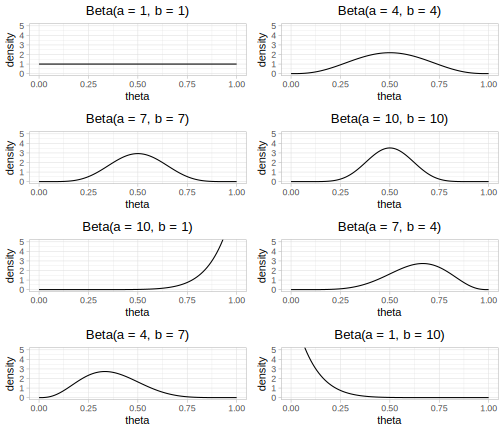
\includegraphics{bookdown_files/figure-latex/betas2-1.pdf}
\caption{\label{fig:betas2}Examples of beta distributions with different parameters.}
\end{figure}

As in the binomial and normal distributions that we saw in chapter 1, one can analytically derive the formulas for the expectation and variance of the beta distribution. These are:

\begin{equation}
\operatorname{E}[X] = \frac{a}{a+b} \quad \operatorname{Var}(X)=\frac {a \cdot b }{(a + b )^{2}(a + b +1)}
\label{eq:meanvar}
\end{equation}

As an example, choosing \(a=4\) and \(b=4\) would mean that the answer ``umbrella'' is as likely as a different answer, but we are relatively unsure about this. We could express our uncertainty by computing the region over which we are 95\% certain that the value of the parameter lies; this is the \emph{95\% credible interval}. For this, we would use the \texttt{qbeta} function in R; the parameters \(a\) and \(b\) are called \texttt{shape1} and \texttt{shape2} in \texttt{R}.

\begin{Shaded}
\begin{Highlighting}[]
\KeywordTok{qbeta}\NormalTok{(}\KeywordTok{c}\NormalTok{(}\FloatTok{0.025}\NormalTok{, }\FloatTok{0.975}\NormalTok{), }\DataTypeTok{shape1 =} \DecValTok{4}\NormalTok{, }\DataTypeTok{shape2 =} \DecValTok{4}\NormalTok{)}
\end{Highlighting}
\end{Shaded}

\begin{verbatim}
## [1] 0.184 0.816
\end{verbatim}

The credible interval chosen above is an equal-tailed interval: the area below the lower bound and above the upper bound is the same (0.025 in the above case). One could define alternative intervals; for example, in a distribution with only one mode (a unimodal distribution), one could choose to use the narrowest interval that contains the mode. This is called the highest posterior density interval (HDI). In skewed posterior distributions, the equal-tailed credible interval and the HDI will not be identical, because the HDI will have unequal tail probabilities. Some authors, such as Kruschke (\protect\hyperlink{ref-kruschke2014doing}{2014}), prefer to report the HDI. We will use the equal-tailed interval in this book, simply because this is the standard output in \texttt{Stan} and \texttt{brms}.

If we were to choose \(a=10\) and \(b=10\), we would still be assuming that a priori the answer ``umbrella'' is just as likely as some other answer, but now our prior uncertainty about this mean is lower, as the 95\% credible interval computed below shows.

\begin{Shaded}
\begin{Highlighting}[]
\KeywordTok{qbeta}\NormalTok{(}\KeywordTok{c}\NormalTok{(}\FloatTok{0.025}\NormalTok{, }\FloatTok{0.975}\NormalTok{), }\DataTypeTok{shape1 =} \DecValTok{10}\NormalTok{, }\DataTypeTok{shape2 =} \DecValTok{10}\NormalTok{)}
\end{Highlighting}
\end{Shaded}

\begin{verbatim}
## [1] 0.289 0.711
\end{verbatim}

In Figure \ref{fig:betas2}, we can see also the difference in uncertainty in these two examples graphically.

Which prior should we choose? In a real data analysis problem, the choice of prior would depend on what prior knowledge we want to bring into the analysis. If we don't have much prior information, we could use \(a=b=1\); this gives us a uniform prior. This kind of prior goes by various names, such as \emph{flat, non-informative prior}, or \emph{uninformative prior}. By contrast, if we have a lot of prior knowledge and/or a strong belief (e.g., based on a particular theory's predictions, or prior data) that \(\theta\) has a particular range of plausible values, we can use a different set of \(a, b\) values to reflect our belief about the parameter. In the above example, the larger our parameters a and b, the narrower the spread of the distribution; i.e., the lower our uncertainty about the mean value of the parameter.

We will discuss prior specification in detail later in chapter \ref{ch:priors}. For the moment, just for illustration, we choose the values \(a=4\) and \(b=4\) for the beta prior. Then, our prior for \(\theta\) is the following beta PDF:

\begin{equation}
p(\theta) = \frac{1}{B(4,4)} \theta^{3} (1-\theta)^{3}
\end{equation}

Having chosen a likelihood, and having defined a prior on \(\theta\), we are ready to carry out our first Bayesian analysis to derive a posterior distribution for \(\theta\).

\hypertarget{using-bayes-rule-to-compute-the-posterior-pthetank}{%
\subsection{\texorpdfstring{Using Bayes' rule to compute the posterior \(p(\theta|n,k)\)}{Using Bayes' rule to compute the posterior p(\textbackslash{}theta\textbar{}n,k)}}\label{using-bayes-rule-to-compute-the-posterior-pthetank}}

Having specified the likelihood and the prior, we will now use Bayes' rule to calculate \(p(\theta|n,k)\). Using Bayes' rule simply involves replacing the Likelihood and the Prior we defined above into the equation we saw earlier:

\begin{equation}
\hbox{Posterior} = \frac{\hbox{Likelihood} \cdot \hbox{Prior}}{\hbox{Marginal Likelihood}}
\end{equation}

Replace the terms for likelihood and prior into this equation:

\begin{equation}
p(\theta|n=100,k=80) = \frac{\left[\binom{100}{80} \theta^{80} \cdot (1-\theta)^{20}\right]  \times \left[\frac{1}{B(4,4)} \times \theta^{3} (1-\theta)^{3}\right]}{p(k=80)}
\label{eq:betaunpost}
\end{equation}

where \(p(k=80)\) is \(\int_{0}^1 p(k=80|n=100,\theta) p(\theta)\, d\theta\). This term will be a constant once the number of successes \(k\) is known; this is the marginal likelihood we encountered in chapter 1. In fact, once \(k\) is known, there are several constant values in the above equation; they are constants because none of them depend on the parameter of interest, \(\theta\). We can collect all of these together:

\begin{equation}
p(\theta|n=100,k=80) =   \left[ \frac{\binom{100}{80}}{B(4,4)\times p(k=80)} \right]   [\theta^{80} (1-\theta)^{20} \times  \theta^{3} (1-\theta)^{3}]
\label{eq:betaunpost2}
\end{equation}

The first term that is in square brackets, \(\frac{\binom{100}{80}}{B(4,4)\times p(k=80)}\), is all the constants collected together, and is the normalizing constant we have seen before; it makes the posterior distribution \(p(\theta|n=100,k=80)\) sum to one. Since it is a constant, we can ignore it for now and focus on the two other terms in the equation. Because we are ignoring the constant, we will now say that the posterior is proportional to the right-hand side.

\begin{equation}
p(\theta|n=100,k=80) \propto   [\theta^{80} (1-\theta)^{20} \times \theta^{3} (1-\theta)^{3} ]
\label{eq:betaunpost3}
\end{equation}

A common way of writing the above equation is:

\begin{equation}
\hbox{Posterior} \propto \hbox{Likelihood} \times \hbox{Prior}
\end{equation}

Resolving the right-hand side now simply involves adding up the exponents! In this example, computing the posterior really does boil down to this simple addition operation on the exponents.

\begin{equation}
p(\theta|n=100,k=80) \propto   [\theta^{80+3} (1-\theta)^{20+3}] = \theta^{83} (1-\theta)^{23}
\label{eq:betaunpost4}
\end{equation}

The expression on the right-hand side corresponds to a beta distribution with parameters \(a=84\), and \(b=24\). This becomes evident if we rewrite the right-hand side such that it represents the core part of a beta PDF (see equation \eqref{eq:beta}). All that is missing is a normalizing constant which would make the area under the curve sum to one.

\begin{equation}
\theta^{83} (1-\theta)^{23} = \theta^{84-1} (1-\theta)^{24-1} 
\end{equation}

This core part of any PDF or PMF is called the kernel of that distribution. Without a normalizing constant, the area under the curve will not sum to one. Let's check this:

\begin{Shaded}
\begin{Highlighting}[]
\NormalTok{PostFun <-}\StringTok{ }\ControlFlowTok{function}\NormalTok{(theta) \{}
\NormalTok{  theta}\OperatorTok{^}\DecValTok{83} \OperatorTok{*}\StringTok{ }\NormalTok{(}\DecValTok{1} \OperatorTok{-}\StringTok{ }\NormalTok{theta)}\OperatorTok{^}\DecValTok{23}
\NormalTok{\}}
\NormalTok{(AUC <-}\StringTok{ }\KeywordTok{integrate}\NormalTok{(PostFun, }\DataTypeTok{lower =} \DecValTok{0}\NormalTok{, }\DataTypeTok{upper =} \DecValTok{1}\NormalTok{)}\OperatorTok{$}\NormalTok{value)}
\end{Highlighting}
\end{Shaded}

\begin{verbatim}
## [1] 8.32e-26
\end{verbatim}

So the area under the curve (AUC) is not 1---the posterior that we computed above is not a proper probability distribution.

All that is needed to make this into a proper probability distribution is to include a normalizing constant, which, according to the definition of the beta distribution, would be \(B(84,24)\). This term is in fact the integral we computed above.

\begin{equation}
p(\theta|n=100,k=80) = \frac{1}{B(84,24)} \theta^{84-1} (1-\theta)^{24-1} 
\end{equation}

Now, this function will sum to one:

\begin{Shaded}
\begin{Highlighting}[]
\NormalTok{PostFun <-}\StringTok{ }\ControlFlowTok{function}\NormalTok{(theta) \{}
\NormalTok{  theta}\OperatorTok{^}\DecValTok{83} \OperatorTok{*}\StringTok{ }\NormalTok{(}\DecValTok{1} \OperatorTok{-}\StringTok{ }\NormalTok{theta)}\OperatorTok{^}\DecValTok{23} \OperatorTok{/}\StringTok{ }\NormalTok{AUC}
\NormalTok{\}}
\KeywordTok{integrate}\NormalTok{(PostFun, }\DataTypeTok{lower =} \DecValTok{0}\NormalTok{, }\DataTypeTok{upper =} \DecValTok{1}\NormalTok{)}\OperatorTok{$}\NormalTok{value}
\end{Highlighting}
\end{Shaded}

\begin{verbatim}
## [1] 1
\end{verbatim}

\hypertarget{summary-of-the-procedure}{%
\subsection{Summary of the procedure}\label{summary-of-the-procedure}}

To summarize, we started with a binomial likelihood, multiplied it with the prior \(\theta \sim \mathit{Beta}(4,4)\), and obtained the posterior \(p(\theta|n,k) \sim \mathit{Beta}(84,24)\). The constants were ignored when carrying out the multiplication; we say that we computed the posterior \emph{up to proportionality}. Finally, we showed how, in this simple example, the posterior can be rescaled to become a probability distribution, by including a proportionality constant.

The above example is a case of a \emph{conjugate} analysis: the posterior on the parameter has the same form as the prior. The above combination of likelihood and prior is called the beta-binomial conjugate case. There are several other such combinations of Likelihoods and Priors that yield a posterior that has the same PDF as the prior on the parameter; some examples will appear in the exercises.

Formally, conjugacy is defined as follows: Given the likelihood \(p(y| \theta)\), if the prior \(p(\theta)\) results in a posterior \(p(\theta|y)\) that has the same form as \(p(\theta)\), then we call \(p(\theta)\) a conjugate prior.

For the beta-binomial conjugate case, we can derive a very general relationship between the likelihood, prior, and posterior. Given the binomial likelihood up to proportionality (ignoring the constant) \(\theta^k (1-\theta)^{n-k}\), and given the prior, also up to proportionality, \(\theta^{a-1} (1-\theta)^{b-1}\), their product will be:

\begin{equation}
\theta^k (1-\theta)^{n-k} \theta^{a-1} (1-\theta)^{b-1} = \theta^{a+k-1} (1-\theta)^{b+n-k-1} 
\end{equation}

Thus, given a \(\mathit{Binomial}(n,k|\theta)\) likelihood, and a \(\mathit{Beta}(a,b)\) prior on \(\theta\), the posterior will be \(\mathit{Beta}(a+k,b+n-k)\).

\hypertarget{visualizing-the-prior-likelihood-and-the-posterior}{%
\subsection{Visualizing the prior, likelihood, and the posterior}\label{visualizing-the-prior-likelihood-and-the-posterior}}

We established in the example above that the posterior is a beta distribution with parameters \(a=84\), and \(b = 24\). We visualize the likelihood, prior, and the posterior alongside each other in Figure \ref{fig:postbeta-viz}.



\begin{figure}
\centering
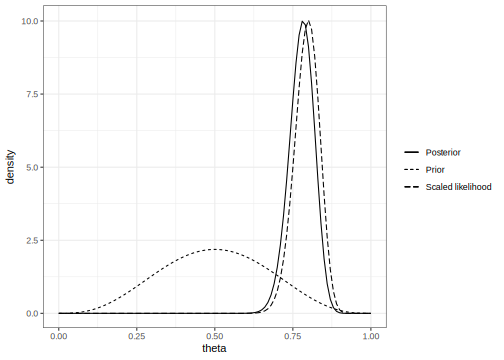
\includegraphics{bookdown_files/figure-latex/postbeta-viz-1.pdf}
\caption{\label{fig:postbeta-viz}The (scaled) likelihood, prior, and posterior in the beta-binomial conjugate example. The likelihood is scaled to integrate to 1 to make it easier to compare to the prior and posterior distributions.}
\end{figure}

We can summarize the posterior distribution either graphically as we did above, or summarize it by computing the mean and the variance. The mean gives us an estimate of the cloze probability of producing ``umbrella'' in that sentence (given the model, i.e., given the likelihood and prior):

\begin{equation}
\operatorname{E}[\hat\theta] = \frac{84}{84+24}=0.78
\label{eq:meanPb}
\end{equation}

\begin{equation}
\operatorname{var}[\hat\theta]=\frac {84 \cdot 24 }{(84+24 )^{2}(84+24 +1)}= 0.0016
\label{eq:varPb}
\end{equation}

We could also display the 95\% credible interval, the range over which we are 95\% certain the true value of \(\theta\) lies, given the data and model.

\begin{Shaded}
\begin{Highlighting}[]
\KeywordTok{qbeta}\NormalTok{(}\KeywordTok{c}\NormalTok{(}\FloatTok{0.025}\NormalTok{, }\FloatTok{0.975}\NormalTok{), }\DataTypeTok{shape1 =} \DecValTok{84}\NormalTok{, }\DataTypeTok{shape2 =} \DecValTok{24}\NormalTok{)}
\end{Highlighting}
\end{Shaded}

\begin{verbatim}
## [1] 0.695 0.851
\end{verbatim}

Typically, we would summarize the results of a Bayesian analysis by displaying the posterior distribution of the parameter (or parameters) graphically, along with the above summary statistics: the mean, the standard deviation or variance, and the 95\% credible interval. You will see many examples of such summaries later.

\hypertarget{the-posterior-distribution-is-a-compromise-between-the-prior-and-the-likelihood}{%
\subsection{The posterior distribution is a compromise between the prior and the likelihood}\label{the-posterior-distribution-is-a-compromise-between-the-prior-and-the-likelihood}}

Just for the sake of illustration, let's take four different beta priors, each reflecting increasing certainty.

\begin{itemize}
\tightlist
\item
  \(\mathit{Beta}(a=2,b=2)\)
\item
  \(\mathit{Beta}(a=3,b=3)\)
\item
  \(\mathit{Beta}(a=6,b=6)\)
\item
  \(\mathit{Beta}(a=21,b=21)\)
\end{itemize}

Each prior reflects a belief that \(\theta=0.5\), with varying degrees of (un)certainty. Given the general formula we developed above for the beta-binomial case, we just need to plug in the likelihood and the prior to get the posterior:

\begin{equation}
p(\theta | n,k) \propto p(k |n,\theta) p(\theta)
\end{equation}

The four corresponding posterior distributions would be:

\begin{equation}
p(\theta\mid k,n) \propto [\theta^{80} (1-\theta)^{20}] [\theta^{2-1}(1-\theta)^{2-1}] = \theta^{82-1} (1-\theta)^{22-1}
\end{equation}

\begin{equation}
p(\theta\mid k,n) \propto [\theta^{80} (1-\theta)^{20}] [\theta^{3-1}(1-\theta)^{3-1}] = \theta^{83-1} (1-\theta)^{23-1}
\end{equation}

\begin{equation}
p(\theta\mid k,n) \propto [\theta^{80} (1-\theta)^{20}] [\theta^{6-1}(1-\theta)^{6-1}] = \theta^{86-1} (1-\theta)^{26-1}
\end{equation}

\begin{equation}
p(\theta\mid k,n) \propto [\theta^{80} (1-\theta)^{20}] [\theta^{21-1}(1-\theta)^{21-1}] = \theta^{101-1} (1-\theta)^{41-1}
\end{equation}

We can visualize each of these triplets of priors, likelihoods and posteriors; see Figure \ref{fig:postbetavizvar}.

\begin{figure}
\centering
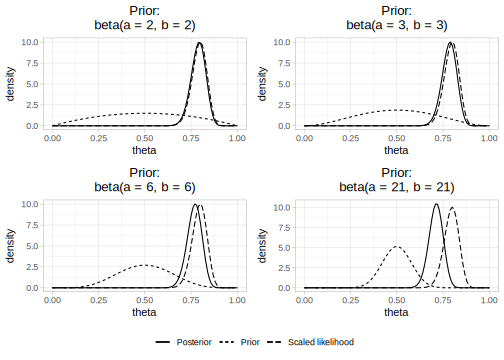
\includegraphics{bookdown_files/figure-latex/postbetavizvar-1.pdf}
\caption{\label{fig:postbetavizvar}The (scaled) likelihood, prior, and posterior in the beta-binomial conjugate example, for different uncertainties in the prior. The likelihood is scaled to integrate to 1 to make its comparison easier.}
\end{figure}

If you hold the likelihood function constant (held constant at \(n=100, k=80\) in the above example), the tighter the prior, the greater the extent to which the posterior orients itself towards the prior. In general, we can say the following about the likelihood-prior-posterior relationship:

\begin{itemize}
\tightlist
\item
  The posterior distribution is a compromise between the prior and the likelihood.
\item
  For a given set of data, the greater the certainty in the prior, the more heavily the posterior will be influenced by the prior mean.
\item
  Conversely, for a given set of data, the greater the \emph{un}certainty in the prior, the more heavily the posterior will be influenced by the likelihood.
\end{itemize}

Another important observation emerges if we increase the sample size from \(100\) to, say, \(1000000\). Suppose we still get a sample mean of \(0.8\) here, so that \(k=800000\). Now, the posterior mean will be influenced almost entirely by the sample mean. This is because, in the general form for the posterior \(\mathit{Beta}(a+k,b+n-k)\) that we computed above, the \(n\) and \(k\) become very large relative to the a, b values, and dominate in determining the posterior mean.

Whenever we do a Bayesian analysis, it is good practice to check whether the parameter you are interested in estimating is sensitive to the prior specification. Such an investigation is called a \emph{sensitivity analysis}. Later in this book, we will see many examples of sensitivity analyses in realistic data-analysis settings.

\hypertarget{incremental-knowledge-gain-using-prior-knowledge}{%
\subsection{Incremental knowledge gain using prior knowledge}\label{incremental-knowledge-gain-using-prior-knowledge}}

In the above example, we used an artificial example where we asked \(100\) subjects to complete the sentence shown at the beginning of the chapter, and then we counted the number of times that they produced ``umbrella'' vs.~some other word as a continuation. Given 80 instances of ``umbrella'', and using a \(\mathit{Beta}(4,4)\) prior, we derived the posterior to be \(\mathit{Beta}(84,24)\). We could now use this posterior as our prior for the next study. Suppose that we were to carry out a second experiment, again with 100 subjects, and this time \(60\) produced ``umbrella''. We could now use our new prior (\(\mathit{Beta}(84,24)\)) to obtain an updated posterior. We have \(a=84, b=24, n=100, k=60\). This gives us as posterior:
\(\mathit{Beta}(a+k,b+n-k) = \mathit{Beta}(84+60,24+100-60)=\mathit{Beta}(144,64)\).

Now, if we were to pool all our data that we have from the two experiments, then we would have as data \(n=200, k=140\). Suppose that we keep our initial prior of \(a=4,b=4\). Then, our posterior would be \(\mathit{Beta}(4+140,4+200-140)=\mathit{Beta}(144,64)\). This is exactly the same posterior that we got when first analyzed the first \(100\) subjects' data, derived the posterior, and then used that posterior as a prior for the next \(100\) subjects' data.

This toy example illustrates an important point that has great practical importance for cognitive science. One can incrementally gain information about a research question by using information from previous studies and deriving a posterior, and then use that posterior as a prior. For practical examples from psycholinguistics showing how information can be pooled from previous studies, see Jäger, Engelmann, and Vasishth (\protect\hyperlink{ref-JaegerEngelmannVasishth2017}{2017}) and Nicenboim, Roettger, and Vasishth (\protect\hyperlink{ref-NicenboimRoettgeretal}{2018}). Vasishth and Engelmann (\protect\hyperlink{ref-VasishthEngelmann2022}{2022}) illustrates an example of how the posterior from a previous study or collection of studies can be used to compute the posterior derived from new data.

\hypertarget{summary-1}{%
\section{Summary}\label{summary-1}}

In this chapter, we learned how to use Bayes' rule in the specific case of a binomial likelihood, and a beta prior on the \(\theta\) parameter in the likelihood function. Our goal in any Bayesian analysis will follow the path we took in this simple example: decide on an appropriate likelihood function, decide on priors for all the parameters involved in the likelihood function, and using this model (i.e., the likelihood and the priors) derive the posterior distribution of each parameter. Then we draw inferences about our research question based on the posterior distribution of the parameter.

In the example discussed in this chapter, Bayesian analysis was easy. This was because we considered the simple conjugate case of the beta-binomial. In realistic data-analysis settings, our likelihood function will be very complex, and many parameters will be involved. Multiplying the likelihood function and the priors will become mathematically difficult or impossible. For such situations, we use computational methods to obtain samples from the posterior distributions of the parameters.

\hypertarget{further-reading-1}{%
\section{Further reading}\label{further-reading-1}}

Accessible introductions to conjugate Bayesian analysis are
Lynch (\protect\hyperlink{ref-lynch2007introduction}{2007}), and Lunn et al. (\protect\hyperlink{ref-lunn2012bugs}{2012}). Somewhat more demanding discussions of conjugate analysis are in Lee (\protect\hyperlink{ref-lee2012bayesian}{2012}), Carlin and Louis (\protect\hyperlink{ref-carlin2008bayesian}{2008}), Christensen et al. (\protect\hyperlink{ref-christensen2011}{2011}), O'Hagan and Forster (\protect\hyperlink{ref-kendall2004}{2004}) and Bernardo and Smith (\protect\hyperlink{ref-bernardosmith}{2009}).

\hypertarget{sec:BDAexercises}{%
\section{Exercises}\label{sec:BDAexercises}}

\begin{exercise}
\protect\hypertarget{exr:BDAexercisesDerivingBayes}{}{\label{exr:BDAexercisesDerivingBayes} }Deriving Bayes' rule
\end{exercise}

Let \(A\) and \(B\) be two observable events. \(P(A)\) is the probability that \(A\) occurs, and \(P(B)\) is the probability that \(B\) occurs. \(P(A|B)\) is the conditional probability that \(A\) occurs given that \(B\) has happened. \(P(A,B)\) is the joint probability of \(A\) and \(B\) both occurring.

You are given the definition of conditional probability:

\begin{equation}
P(A|B)= \frac{P(A,B)}{P(B)} \hbox{ where } P(B)>0
\end{equation}

Using the above definition, and using the fact that \(P(A,B)=P(B,A)\) (i.e., the probability of \(A\) and \(B\) both occurring is the same as the probability of \(B\) and \(A\) both occurring),
derive an expression for \(P(B|A)\). Show the steps clearly in the derivation.

\begin{exercise}
\protect\hypertarget{exr:BDAexercisesConj1}{}{\label{exr:BDAexercisesConj1} }Conjugate forms 1
\end{exercise}

\begin{itemize}
\tightlist
\item
  Computing the general form of a PDF for a posterior
\end{itemize}

Suppose you are given data \(k\) consisting of the number of successes, coming from a \(\mathit{Binomial}(n,\theta)\) distribution.
Given \(k\) successes in n trials coming from a binomial distribution, we define a \(\mathit{Beta}(a,b)\) prior on the parameter \(\theta\).

Write down the Beta distribution that represents the posterior, in terms of \(a,b, n,\) and \(k\).

\begin{itemize}
\tightlist
\item
  Practical application
\end{itemize}

We ask 10 yes/no questions from a subject, and the subject returns 0 correct answers. We assume a binomial likelihood function for these data. Also assume a \(\mathit{Beta}(1,1)\) prior on the parameter \(\theta\), which represents the probability of success. Use the result you derived above to write down the posterior distribution of the \(\theta\) parameter.

\begin{exercise}
\protect\hypertarget{exr:BDAexercisesConj2}{}{\label{exr:BDAexercisesConj2} }Conjugate forms 2
\end{exercise}

Suppose you have \(n\) independent and identically distributed data points from the Geometric distribution, which has
the likelihood function

\begin{equation}
f(x|\theta)=\theta(1-\theta)^{\sum_{i=1}^n x_i}
\end{equation}

where the data points \(x\) can have values 0,1,2,\dots. Let the prior on \(\theta\) be \(\mathit{Beta}(a,b)\), a beta distribution with parameters a,b.
The posterior distribution is a beta distribution with parameters a* and b*. Determine these parameters in terms of \(a\), \(b\), and \(\sum_{i=1}^n x_i\).

\begin{exercise}
\protect\hypertarget{exr:BDAexercisesConj3}{}{\label{exr:BDAexercisesConj3} }Conjugate forms 3
\end{exercise}

The Gamma distribution is defined in terms of the parameters a, b: Ga(a,b). Given some data \(x\), the probability density function is:

\begin{equation}
Ga(x | a,b)=\frac{b^a x^{a-1} \exp\{-bx\}}{\Gamma(a)}
\end{equation}

We have data \(x_1,\dots, x_n\), with sample size \(n\) that is exponentially distributed. The exponential likelihood function is:

\begin{equation}
p(x_1,\dots,x_n | \lambda)=\lambda^n \exp \{-\lambda \sum_{i=1}^n x_i \}
\end{equation}

It turns out that if we assume a Ga(a,b) prior distribution and the above Exponential likelihood, the posterior distribution of \(\lambda\) is a Gamma distribution. In other words, the Gamma(a,b) prior on the \(\lambda\) parameter in the Exponential distribution will be written:

\begin{equation}
Ga(\lambda | a,b)=\frac{b^a \lambda^{a-1} \exp\{-b\lambda\}}{\Gamma(a)}
\end{equation}

Find the parameters \(a'\) and \(b'\) of the posterior distribution.

\begin{exercise}
\protect\hypertarget{exr:BDAexercisesConj4}{}{\label{exr:BDAexercisesConj4} }Conjugate forms 4
\end{exercise}

\begin{itemize}
\tightlist
\item
  Computing the posterior
\end{itemize}

This is a contrived example. Suppose we are modeling the number of times that a speaker says the word ``I'' per day. This could be of interest if we are studying, for example, how self-oriented a speaker is. The number of times \(x\) that the word is uttered in over a particular time period (here, one day) can be modeled by a Poisson distribution:

\begin{equation}
f(x\mid \theta) = \frac{\exp(-\theta) \theta^x}{x!}
\end{equation}

where the rate \(\theta\) is unknown, and the numbers of utterances of the target word on each day are independent given \(\theta\).

We are told that the prior mean of \(\theta\) is 100 and prior variance for \(\theta\) is 225. This information is based on the results of previous studies on the topic. We will use the Gamma(a,b) density (see previous question) as a prior for \(\theta\) because this is a conjugate prior to the Poisson distribution.

\begin{enumerate}
\def\labelenumi{\alph{enumi})}
\tightlist
\item
  First, visualize the prior, a Gamma density prior for \(\theta\) based on the above information.
\end{enumerate}

{[}Hint: we know that for a Gamma density with parameters a, b, the mean is \(\frac{a}{b}\) and the variance is \(\frac{a}{b^2}\). Since we are given values for the mean and variance, we can solve for a,b, which gives us the Gamma density.{]}

\begin{enumerate}
\def\labelenumi{\alph{enumi})}
\setcounter{enumi}{1}
\tightlist
\item
  Next, derive the posterior distribution of the parameter \(\theta\) up to proportionality, and write down the posterior distribution in terms of the parameters of a Gamma distribution.
\end{enumerate}

\begin{itemize}
\tightlist
\item
  Practical application
\end{itemize}

Suppose we know that the number of ``I'' utterances from a particular individual is \(115, 97, 79, 131\). Use the result you derived above to obtain the posterior distribution. In other words, write down the a,b parameters of the Gamma distribution representing the posterior distribution of \(\theta\).

Plot the prior, likelihood, and the posterior alongside each other.

Now suppose you get one new data point: 200. Write down the updated posterior (the a,b parameters of the Gamma distribution) given this new data point. Add the updated posterior to the plot you made above.

\begin{exercise}
\protect\hypertarget{exr:BDAexercisesWeightedMean}{}{\label{exr:BDAexercisesWeightedMean} }The posterior mean is a weighted mean of the prior mean and the MLE (Poisson-Gamma conjugate case)
\end{exercise}

The number of times an event happens per unit time can be modeled using a Poisson distribution, whose PMF is:

\begin{equation}
f(x\mid \theta) = \frac{\exp(-\theta) \theta^x}{x!}
\end{equation}

Suppose that we define a Gamma(a,b) prior for the rate parameter \(\theta\). It is a fact (see exercises above) that the posterior of the \(\theta\) parameter is a \(Gamma(a*,b*)\) distribution, where \(a*\) and \(b*\) are the updated hyperparameters given the data: \(\theta \sim Gamma(a*,b*)\).

\begin{itemize}
\tightlist
\item
  Prove that the posterior mean is a weighted mean of the prior mean and the maximum likelihood estimate (mean) of the Poisson-distributed data, \(\bar{x} = \sum_{i=1}^n x/n\). Hint: the mean of a Gamma distribution is \(\frac{a}{b}\).
\end{itemize}

Specifically, what you have to prove is that:

\begin{equation} 
\frac{a*}{b*} = \frac{a}{b} \times \frac{w_1}{w_1 + w_2} + \bar{x} \times \frac{w_2}{w_1 + w_2} 
\label{eq:weightingpoisga}
\end{equation}

where \(w_1 = 1\) and \(w_2=\frac{n}{b}\).

\begin{itemize}
\item
  Given equation \eqref{eq:weightingpoisga}, show that as \(n\) increases (as sample size goes up), the maximum likelihood estimate \(\bar{x}\) dominates in determining the posterior mean, and when \(n\) gets smaller and smaller, the prior mean dominates in determining the posterior mean.
\item
  Finally, given that the variance of a Gamma distribution is \(\frac{a}{b^2}\), show that as \(n\) increases, the posterior variance will get smaller and smaller (the uncertainty on the posterior will go down).
\end{itemize}

\hypertarget{part-regression-models-with-brms}{%
\part{Regression models with brms}\label{part-regression-models-with-brms}}

\hypertarget{ch:compbda}{%
\chapter{Computational Bayesian data analysis}\label{ch:compbda}}

In the previous chapter, we learned how to analytically derive the posterior distribution of the parameters in our model.
In practice, however, this is possible for only a very limited number of cases. Although the numerator of the Bayes rule, the unnormalized posterior, is easy to calculate (by multiplying the probability density/mass functions analytically), the denominator, the marginal likelihood, requires us to carry out an integration; see \eqref{eq:bayesbrms}.

\begin{equation}
\begin{aligned}
p(\boldsymbol{\Theta}|\boldsymbol{y}) &= \cfrac{ p(\boldsymbol{y}|\boldsymbol{\Theta}) \cdot p(\boldsymbol{\Theta}) }{p(\boldsymbol{y})}\\
p(\boldsymbol{\Theta}|\boldsymbol{y}) &= \cfrac{ p(\boldsymbol{y}|\boldsymbol{\Theta}) \cdot p(\boldsymbol{\Theta}) }{\int_{\boldsymbol{\Theta}} p(\boldsymbol{y}|\boldsymbol{\Theta}) \cdot p(\boldsymbol{\Theta}) d\boldsymbol{\Theta} }
\end{aligned}
\label{eq:bayesbrms}
\end{equation}

Unless we are dealing with conjugate distributions, the solution will be extremely hard to derive or there will be no analytical solution. This was the major bottleneck of Bayesian analysis in the past, and required Bayesian practitioners to program an approximation method by themselves before they could even begin the Bayesian analysis. Fortunately, many of the probabilistic programming languages freely available today (see the next section for a listing) allow us to define our models without having to acquire expert knowledge about the relevant numerical techniques.

\hypertarget{sec:sampling}{%
\section{Deriving the posterior through sampling}\label{sec:sampling}}

Let's say that we want to derive the posterior of the model from section \ref{sec:analytical}, that is, the posterior distribution of the cloze probability of \emph{``umbrella''}, \(\theta\), given the following data: a word (e.g., \emph{``umbrella''}) was answered 80 out of 100 times, and assuming a binomial distribution as the likelihood function, and \(\mathit{Beta}(a=4,b=4)\) as a prior distribution for the cloze probability. If we can obtain samples from the posterior distribution of \(\theta\), instead of an analytically derived posterior distribution, given enough samples we will have a good approximation of the posterior distribution. Obtaining samples from the posterior will be the only viable option in the models that we will discuss in this book. By ``obtaining samples'', we are talking about a situation analogous to when we use \texttt{rbinom} or \texttt{rnorm} to obtain samples from a particular distribution. For more details about sampling algorithms, see the further readings suggested in section \ref{sec:ch3furtherreading}.

Thanks to probabilistic programming languages, it will be relatively straightforward to get these samples, and we will discuss how we will do it in more detail in the next section. For now let's assume that we used some probabilistic programming language to obtain 20000 samples from the posterior distribution of the cloze probability, \(\theta\): 0.758, 0.779, 0.761, 0.79, 0.735, 0.855, 0.782, 0.756, 0.835, 0.755, 0.837, 0.736, 0.799, 0.777, 0.875, 0.764, 0.784, 0.756, 0.793, 0.794, \ldots{} Figure \ref{fig:betapost} shows that the approximation of the posterior looks quite similar to the analytically derived posterior. The difference between the analytically computed and approximated mean and variance are -0.0002 and 0.00001 respectively.



\begin{figure}
\centering
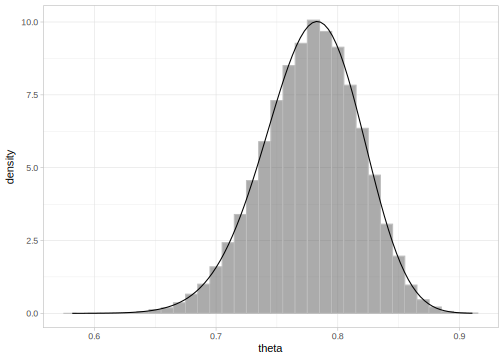
\includegraphics{bookdown_files/figure-latex/betapost-1.pdf}
\caption{\label{fig:betapost}Histogram of the samples of \(\theta\) from the posterior distribution generated via sampling. The black line shows the density plot of the analytically derived posterior.}
\end{figure}

\hypertarget{bayesian-regression-models-using-stan-brms}{%
\subsection{Bayesian Regression Models using Stan: brms}\label{bayesian-regression-models-using-stan-brms}}

The surge in popularity of Bayesian statistics is closely tied to the increase in computing power and the appearance of probabilistic programming languages, such as WinBUGS (Lunn et al. \protect\hyperlink{ref-lunn2000winbugs}{2000}), JAGS (Plummer \protect\hyperlink{ref-plummer2016jags}{2016}), R-INLA (Lindgren and Rue \protect\hyperlink{ref-lindgren2015bayesian}{2015}), pymc3 (Salvatier, Wiecki, and Fonnesbeck \protect\hyperlink{ref-Salvatier2016}{2016}), Turing (Ge, Xu, and Ghahramani \protect\hyperlink{ref-turing}{2018}), and Stan (Carpenter et al. \protect\hyperlink{ref-carpenter2017stan}{2017}). These probabilistic programming languages allow the user to define models without having to deal (for the most part) with the complexities of the sampling process. However, they require learning a new language since the user has to fully specify the statistical model using a particular syntax.\footnote{The Python package pymc3 and the Julia library Turing are recent exceptions since they are fully integrated into their respective languages.} Furthermore, some knowledge of the sampling process is needed to correctly parametrize the models and to avoid convergence issues (these topics will be covered in detail later in this book).

There are some alternatives that allow Bayesian inference in \texttt{R} without having to fully specify the model ``by hand''. The packages \texttt{rstanarm} (Goodrich et al. \protect\hyperlink{ref-rstanarm}{2018}) and \texttt{brms} (Bürkner \protect\hyperlink{ref-R-brms}{2019}) provide Bayesian equivalents of many popular R model-fitting functions, such as (g)lmer (Bates, Mächler, et al. \protect\hyperlink{ref-R-lme4}{2015}\protect\hyperlink{ref-R-lme4}{b}); both \texttt{rstanarm} and \texttt{brms} use Stan as the back-end for estimation and sampling. Another new alternative is JASP (JASP Team \protect\hyperlink{ref-JASP2019}{2019}), which provides a graphical user interface for both frequentist and Bayesian modeling, and is intended to be an open-source alternative to SPSS.

We will focus on \texttt{brms} in the first two parts of the book. This is because it can be useful for a smooth transition from frequentist models to their Bayesian equivalents. Although \texttt{brms} is powerful enough to satisfy the statistical needs of many cognitive scientists, it has the added benefit that the Stan code can be inspected (with the \texttt{brms} functions \texttt{make\_stancode} and \texttt{make\_standata}), allowing the users to customize their models or learn from the code produced internally by \texttt{brms} to eventually transition to writing the models entirely in Stan. We revisit the models of this chapter and the following one in the introduction to Stan in chapter \ref{ch:introstan}.

\hypertarget{sec:simplenormal}{%
\subsubsection{A simple linear model: A single subject pressing a button repeatedly}\label{sec:simplenormal}}

We'll use the following example to illustrate the basic steps for fitting a model. Let's say we have data from a subject repeatedly pressing the space bar as fast as possible, without paying attention to any stimuli. The data are response times in milliseconds in each trial. We would like to know how long it takes to press a key when there is no decision involved.

Let's model the data with the following assumptions:

\begin{enumerate}
\def\labelenumi{\arabic{enumi}.}
\tightlist
\item
  There is a true (unknown) underlying time, \(\mu\) ms, that the subject needs to press the space bar.
\item
  There is some noise in this process.
\item
  The noise is normally distributed (this assumption is questionable given that response times are generally skewed; we will fix this assumption later).
\end{enumerate}

This means that the likelihood for each observation \(n\) will be:

\begin{equation}
rt_n \sim \mathit{Normal}(\mu, \sigma)
\label{eq:rtlik}
\end{equation}

where \(n =1, \ldots, N\), and \(rt\) is the dependent variable (response times in milliseconds). The variable \(N\) indexes the total number of data points. The symbol \(\mu\) indicates the \emph{location} of the normal distribution function; the location parameter shifts the distribution left or right on the horizontal axis. For the normal distribution, the location is also the mean of the distribution. The symbol \(\sigma\) indicates the \emph{scale} of the distribution; as the scale decreases, the distribution gets narrower. This compressing approaches a spike (all the probability mass get concentrated near one point) as the scale parameter approached zero. For the normal distribution, the scale is also its standard deviation.

The reader may have encountered the model shown in Equation \eqref{eq:rtlik} in the form shown in Equation \eqref{eq:rtlikLM}:

\begin{equation}
rt_n = \mu + \varepsilon \hbox{, where } \varepsilon_n \stackrel{iid}{\sim} \mathit{Normal}(0,\sigma) \label{eq:rtlikLM} 
\end{equation}

When the model is written in this way, it should be understood as meaning that each data point \(rt_n\) has some variability around a mean value \(\mu\), and that variability has standard deviation \(\sigma\). The term ``iid'' (independent and identically distributed) implies that each data point \(rt_n\) is independently generated (is not correlated with any of the other data points), and is coming from the same distribution (namely, \(Normal(\mu,\sigma)\)).

For a frequentist model that will give us the maximum likelihood estimate (the sample mean) of the time it takes to press the space bar, this would be enough information to write the formula in \texttt{R}, \texttt{rt\ \textasciitilde{}\ 1}, and plug it into the function \texttt{lm()} together with the data: \texttt{lm(rt\ \textasciitilde{}\ 1,\ data)}. The meaning of the \texttt{1} here is that \texttt{lm} will estimate the intercept in the model, in our case \(\mu\). If the reader is completely unfamiliar with linear models, the references in section \ref{sec:ch4furtherreading} will be helpful.

For a Bayesian linear model, we will also need to define priors for the two parameters of our model. Let's say that we know for sure that the time it takes to press a key will be positive and lower than a minute (or 60000ms), but we don't want to make a commitment regarding which values are more likely. We encode what we know about the noise in the task in \(\sigma\): we know that this parameter must be positive and we'll assume that any value below 2000ms is equally likely. These priors are in general strongly discouraged: A flat (or very wide) prior will almost never be the best approximation of what we know. Prior specification will be discussed in detail in chapter \ref{ch:priors}.

In this case, even if we know very little about the task, we know that pressing the spacebar will take at most a couple of seconds. We'll use flat priors in this section for pedagogical purposes; the next chapters will show more realistic uses of priors.

\begin{equation}
\begin{aligned}
\mu &\sim \mathit{Uniform}(0, 60000) \\
\sigma &\sim \mathit{Uniform}(0, 2000) 
\end{aligned}
\label{eq:rtpriors}
\end{equation}

First, load the data frame \texttt{df\_spacebar} from the \texttt{bcogsci} package

\begin{Shaded}
\begin{Highlighting}[]
\KeywordTok{data}\NormalTok{(}\StringTok{"df_spacebar"}\NormalTok{)}
\NormalTok{df_spacebar}
\end{Highlighting}
\end{Shaded}

\begin{verbatim}
## # A tibble: 361 x 2
##      rt trial
##   <int> <int>
## 1   141     1
## 2   138     2
## 3   128     3
## # ... with 358 more rows
\end{verbatim}

It is a good idea to plot the data before doing anything else; see Figure \ref{fig:m1visualize}. As we suspected, the data look a bit skewed, but we ignore this for the moment.

\begin{figure}
\centering
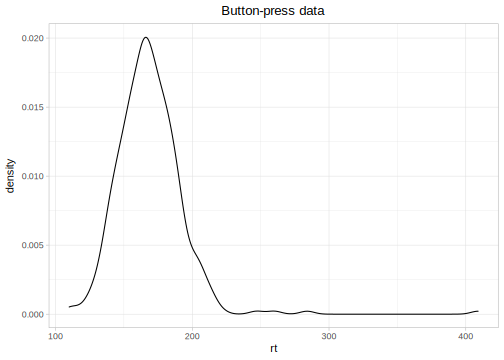
\includegraphics{bookdown_files/figure-latex/m1visualize-1.pdf}
\caption{\label{fig:m1visualize}Visualizing the button-press data.}
\end{figure}

\hypertarget{specifying-the-model-in-brms}{%
\paragraph{\texorpdfstring{Specifying the model in \texttt{brms}}{Specifying the model in brms}}\label{specifying-the-model-in-brms}}

Fit the model defined by Equations \eqref{eq:rtlik} and \eqref{eq:rtpriors} with \texttt{brms} in the following way; as mentioned before, the uniform distribution is not appropriate, and we will ignore this warning \emph{for now}.\footnote{The problem here is that although the parameter for the intercept is assigned a uniform distribution bounded between 0 and 60000 ms, the sampler might start sampling from an initial value outside this range. The sampler can start from an initial value that is outside the 0-60000 range because the initial value is chosen randomly (unless the user specifies an initial value explicitly). For now, it is enough to note that this prior is a bad idea for a model and it's shown here for pedagogical purposes only. \label{fn:uniform}}

\begin{Shaded}
\begin{Highlighting}[]
\NormalTok{fit_press <-}\StringTok{ }\KeywordTok{brm}\NormalTok{(rt }\OperatorTok{~}\StringTok{ }\DecValTok{1}\NormalTok{,}
  \DataTypeTok{data =}\NormalTok{ df_spacebar,}
  \DataTypeTok{family =} \KeywordTok{gaussian}\NormalTok{(),}
  \DataTypeTok{prior =} \KeywordTok{c}\NormalTok{(}
    \KeywordTok{prior}\NormalTok{(}\KeywordTok{uniform}\NormalTok{(}\DecValTok{0}\NormalTok{, }\DecValTok{60000}\NormalTok{), }\DataTypeTok{class =}\NormalTok{ Intercept),}
    \KeywordTok{prior}\NormalTok{(}\KeywordTok{uniform}\NormalTok{(}\DecValTok{0}\NormalTok{, }\DecValTok{2000}\NormalTok{), }\DataTypeTok{class =}\NormalTok{ sigma)}
\NormalTok{  ),}
  \DataTypeTok{chains =} \DecValTok{4}\NormalTok{,}
  \DataTypeTok{iter =} \DecValTok{2000}\NormalTok{,}
  \DataTypeTok{warmup =} \DecValTok{1000}
\NormalTok{)  }
\end{Highlighting}
\end{Shaded}

\begin{verbatim}
## Warning: It appears as if you have specified an upper bounded prior on a parameter that has no natural upper bound.
## If this is really what you want, please specify argument 'ub' of 'set_prior' appropriately.
## Warning occurred for prior 
## sigma ~ uniform(0, 2000)
\end{verbatim}

The \texttt{brms} code has some differences from a model fit with \texttt{lm}. At this beginning stage, we'll focus on the following options:

\begin{enumerate}
\def\labelenumi{\arabic{enumi}.}
\tightlist
\item
  The term \texttt{family\ =\ gaussian()} makes it explicit that the underlying likelihood function is a normal distribution (Gaussian and normal are synonyms). This detail is implicit in \texttt{lm}. Other linking functions are possible, exactly as in the \texttt{glm} function. The default for \texttt{brms} that corresponds to the \texttt{lm} function is \texttt{gaussian()}.
\item
  The term \texttt{prior} takes as argument a vector of priors. Although this specification of priors is optional, the researcher should always explicitly specify each prior. Otherwise, \texttt{brms} will define priors by default, which may or may not be appropriate for the research area.
\item
  The term \texttt{chains} refers to the number of independent runs for sampling (by default four).
\item
  The term \texttt{iter} refers to the number of iterations that the sampler makes to sample from the posterior distribution of each parameter (by default 2000).
\item
  The term \texttt{warmup} refers to the number of iterations from the start of sampling that are eventually discarded (by default half of \texttt{iter}).
\end{enumerate}

The last three options (together with \texttt{control}, which was not used before) determine the behavior of the sampling algorithm: the No-U-Turn Sampler (NUTS; Hoffman and Gelman \protect\hyperlink{ref-hoffmanNoUTurnSamplerAdaptively2014}{2014}) extension of Hamiltonian Monte Carlo (Duane et al. \protect\hyperlink{ref-duaneHybridMonteCarlo1987}{1987}; Neal \protect\hyperlink{ref-nealMCMCUsingHamiltonian2011}{2011}). We will discuss sampling in a bit more depth in chapter \ref{ch:introstan}, but the basic process is explained next.

\hypertarget{sec:convergencenut}{%
\paragraph{Sampling and convergence in a nutshell}\label{sec:convergencenut}}

The code specification starts four chains independently from each other. Each chain ``searches'' for samples of the posterior distribution in a multidimensional space, where each parameter corresponds to a dimension. The shape of this space is determined by the priors and the likelihood. The chains start at random locations, and in each iteration they take one sample each. When sampling begins, the samples may or may not belong to the posterior distributions of the parameters. Eventually, the chains end up in the vicinity of the posterior distribution, and from that point onward the samples will belong to the posterior.

Thus, when sampling begins, the samples from the different chains can be far from each other, but \emph{at some point} they will ``converge'' and start delivering samples from the posterior distributions. Although there are no guarantees that the number of iterations we run the chains for will be sufficient for obtaining samples from the posteriors, the default values of \texttt{brms} (and Stan) are in many cases sufficient to achieve convergence. When the default number of iterations do not suffice, \texttt{brms} (actually, Stan) will print out warnings, with suggestions for fixing the convergence problems. If all the chains converge to the same distribution, by removing the ``warmup'' samples, we make sure that we do not get samples from the initial path to the posterior distributions. The default in \texttt{brms} is that half of the total number of iterations in each chain (which default to 2000) will count as ``warmup''. So, if one runs a model with four chains and the default number of iterations, we will obtain a total of 4000 samples from the four chains, after discarding the warmup iterations.

Figure \ref{fig:warmup} shows the path of the chains from the warmup phase onwards. Such plots are called trace plots or caterpillar plots. The warmup is shown only for illustration purposes; generally, one should only inspect the chains after the point where convergence has (presumably) been achieved (i.e., after the dashed line). After convergence has occurred, a visual diagnostic check is that chains should look like a ``fat hairy caterpillar''. Compare the trace plot of our model in Figure \ref{fig:warmup} with the trace plot of a model that did not converge, shown in Figure \ref{fig:warmup2}.

Trace plots are not always diagnostic as regards convergence. The trace plots might look fine, but the model may not have converged. Fortunately, Stan automatically runs several diagnostics with the information from the chains, and if there are no warnings after fitting the model and the trace plots look fine, we can be reasonably sure that the model converged, and assume that our samples are from the true posterior distribution. However, it is necessary to run more than one chain (preferably four), with a couple of thousands of iterations (at least) in order for the diagnostics to work.



\begin{figure}
\centering
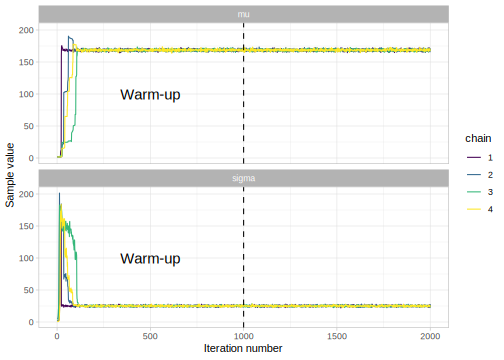
\includegraphics{bookdown_files/figure-latex/warmup-1.pdf}
\caption{\label{fig:warmup}Trace plots of our \texttt{brms} model for the button-pressing data.}
\end{figure}



\begin{figure}
\centering
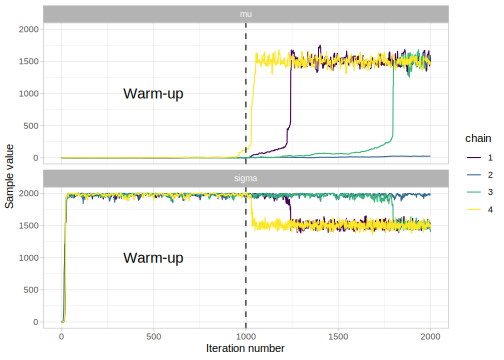
\includegraphics{bookdown_files/figure-latex/warmup2-1.pdf}
\caption{\label{fig:warmup2}Trace plots of a model that \textbf{did not} converge. We can diagnose the non-convergence by the observing that the chains do not overlap---each chain seems to be sampling from a different distribution.}
\end{figure}

\hypertarget{output-of-brms}{%
\paragraph{\texorpdfstring{Output of \texttt{brms}}{Output of brms}}\label{output-of-brms}}

Once the model has been fit (and assuming that we got no warning messages about convergence problems), we can print out the samples of the posterior distributions of each of the parameters:

\begin{Shaded}
\begin{Highlighting}[]
\KeywordTok{as_draws_df}\NormalTok{(fit_press) }
\end{Highlighting}
\end{Shaded}

\begin{verbatim}
## # A draws_df: 1000 iterations, 4 chains, and 3 variables
##    b_Intercept sigma  lp__
## 1          169    24 -1689
## 2          169    25 -1688
## 3          170    25 -1689
## 4          171    24 -1689
## 5          169    25 -1688
## 6          169    24 -1688
## 7          168    25 -1688
## 8          170    25 -1689
## 9          170    25 -1689
## 10         168    23 -1690
## # ... with 3990 more draws
## # ... hidden reserved variables {'.chain', '.iteration', '.draw'}
\end{verbatim}

The term \texttt{b\_Intercept} in the \texttt{brms} output corresponds to our \(\mu\), and \texttt{lp} is not really part of the posterior, it's the density of the unnormalized log posterior for each iteration. \texttt{lp} will be discussed later (in Box \ref{thm:target}).

Plot the density and trace plot of each parameter after the warmup:

\begin{Shaded}
\begin{Highlighting}[]
\KeywordTok{plot}\NormalTok{(fit_press)}
\end{Highlighting}
\end{Shaded}

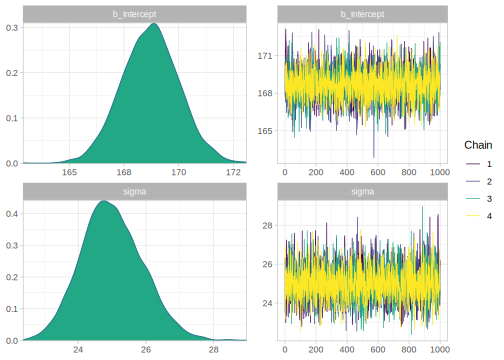
\includegraphics{bookdown_files/figure-latex/unnamed-chunk-36-1.pdf}

\texttt{brms} provides a nice, if somewhat verbose, summary:

\begin{Shaded}
\begin{Highlighting}[]
\NormalTok{fit_press}
\CommentTok{# posterior_summary(fit_press) is also useful}
\end{Highlighting}
\end{Shaded}

\begin{verbatim}
##  Family: gaussian 
##   Links: mu = identity; sigma = identity 
## Formula: rt ~ 1 
##    Data: df_spacebar (Number of observations: 361) 
##   Draws: 4 chains, each with iter = 2000; warmup = 1000; thin = 1;
##          total post-warmup draws = 4000
## 
## Population-Level Effects: 
##           Estimate Est.Error l-95% CI u-95% CI Rhat Bulk_ESS Tail_ESS
## Intercept   168.66      1.30   166.09   171.21 1.00     3150     2674
## 
## Family Specific Parameters: 
##       Estimate Est.Error l-95% CI u-95% CI Rhat Bulk_ESS Tail_ESS
## sigma    24.99      0.93    23.22    26.90 1.00     3584     2674
## 
## Draws were sampled using sampling(NUTS). For each parameter, Bulk_ESS
## and Tail_ESS are effective sample size measures, and Rhat is the potential
## scale reduction factor on split chains (at convergence, Rhat = 1).
\end{verbatim}

The \texttt{Estimate} is just the mean of the posterior sample, and
the CIs mark the lower and upper bounds of the 95\% credible intervals (to distinguish credible intervals from frequentist confidence intervals, the former will be abbreviated as CrIs):

\begin{Shaded}
\begin{Highlighting}[]
\KeywordTok{as_draws_df}\NormalTok{(fit_press)}\OperatorTok{$}\NormalTok{b_Intercept }\OperatorTok\StringTok{ }\KeywordTok{mean}\NormalTok{()}
\end{Highlighting}
\end{Shaded}

\begin{verbatim}
## [1] 169
\end{verbatim}

\begin{Shaded}
\begin{Highlighting}[]
\KeywordTok{as_draws_df}\NormalTok{(fit_press)}\OperatorTok{$}\NormalTok{b_Intercept }\OperatorTok\StringTok{ }\KeywordTok{mean}\NormalTok{()}
\end{Highlighting}
\end{Shaded}

\begin{verbatim}
## [1] 169
\end{verbatim}

\begin{Shaded}
\begin{Highlighting}[]
\KeywordTok{as_draws_df}\NormalTok{(fit_press)}\OperatorTok{$}\NormalTok{b_Intercept }\OperatorTok\StringTok{ }
\StringTok{  }\KeywordTok{quantile}\NormalTok{(}\KeywordTok{c}\NormalTok{(}\FloatTok{0.025}\NormalTok{, }\FloatTok{.975}\NormalTok{))}
\end{Highlighting}
\end{Shaded}

\begin{verbatim}
##  2.5% 97.5% 
##   166   171
\end{verbatim}

We see that we can fit our model without problems, and we get some posterior distributions for our parameters. However, we should ask ourselves the following questions:

\begin{enumerate}
\def\labelenumi{\arabic{enumi}.}
\tightlist
\item
  What information are the priors encoding? Do the priors make sense?
\item
  Does the likelihood assumed in the model make sense for the data?
\end{enumerate}

We'll try to answer these questions by looking at the \emph{Prior and posterior predictive distributions}, and by doing sensitivity analyses as described in the following sections.

\hypertarget{sec:priorpred}{%
\section{Prior predictive distribution}\label{sec:priorpred}}

We had defined the following priors for our linear model:

\begin{equation}
\begin{aligned}
\mu &\sim \mathit{Uniform}(0, 60000) \\
\sigma &\sim \mathit{Uniform}(0, 2000) 
\end{aligned}
\label{eq:rtpriorsrepeated}
\end{equation}

These priors encode assumptions about the kind of data we would expect to see in a future study.
To understand these assumptions, we are going to generate data from the model; such data, which is generated entirely by the prior distributions, is called the prior predictive distribution. Generating prior predictive distributions repeatedly helps us to check whether the priors make sense. What we want to know here is, do the priors generate realistic-looking data?

Formally, we want to know the density \(p(\cdot)\) of data points \(y_{pred_1},\dots,y_{pred_N}\) from a data set \(\boldsymbol{y_{pred}}\) of length \(N\), given a vector of priors \(\boldsymbol{\Theta}\) and our likelihood \(p(\cdot|\boldsymbol{\Theta})\); (in our example, \(\boldsymbol{\Theta}=\langle\mu,\sigma \rangle\)). The prior predictive density is written as follows:

\begin{equation}
\begin{aligned}
p(\boldsymbol{y_{pred}}) &= p(y_{pred_1},\dots,y_{pred_n})\\
&= \int_{\boldsymbol{\Theta}} p(y_{pred_1}|\boldsymbol{\Theta})\cdot p(y_{pred_2}|\boldsymbol{\Theta})\cdots p(y_{pred_N}|\boldsymbol{\Theta}) p(\boldsymbol{\Theta}) \, d\boldsymbol{\Theta} 
\end{aligned}
\end{equation}

In essence, the vector of parameters is integrated out. This yields the probability distribution of possible data sets given the priors and the likelihood, \emph{before any observations are taken into account}.

The integration can be carried out computationally by generating samples from the prior distribution.

Here is one way to generate prior predictive distributions:

Repeat the following many times:

\begin{enumerate}
\def\labelenumi{\arabic{enumi}.}
\tightlist
\item
  Take one sample from each of the priors.
\item
  Plug those samples into the probability density/mass function to generate a data set \(y_{pred_1},\ldots,y_{pred_n}\).
\end{enumerate}

Each sample is an imaginary or potential data set.

Create a function that does this:

\begin{Shaded}
\begin{Highlighting}[]
\NormalTok{normal_predictive_distribution <-}\StringTok{ }
\StringTok{  }\ControlFlowTok{function}\NormalTok{(mu_samples, sigma_samples, N_obs) \{}
  \CommentTok{# empty data frame with headers:}
\NormalTok{  df_pred <-}\StringTok{ }\KeywordTok{tibble}\NormalTok{(}
    \DataTypeTok{trialn =} \KeywordTok{numeric}\NormalTok{(}\DecValTok{0}\NormalTok{),}
    \DataTypeTok{rt_pred =} \KeywordTok{numeric}\NormalTok{(}\DecValTok{0}\NormalTok{),}
    \DataTypeTok{iter =} \KeywordTok{numeric}\NormalTok{(}\DecValTok{0}\NormalTok{)}
\NormalTok{  )}
  \CommentTok{# i iterates from 1 to the length of mu_samples,}
  \CommentTok{# which we assume is identical to}
  \CommentTok{# the length of the sigma_samples:}
  \ControlFlowTok{for}\NormalTok{ (i }\ControlFlowTok{in} \KeywordTok{seq_along}\NormalTok{(mu_samples)) \{}
\NormalTok{    mu <-}\StringTok{ }\NormalTok{mu_samples[i]}
\NormalTok{    sigma <-}\StringTok{ }\NormalTok{sigma_samples[i]}
\NormalTok{    df_pred <-}\StringTok{ }\KeywordTok{bind_rows}\NormalTok{(}
\NormalTok{      df_pred,}
      \KeywordTok{tibble}\NormalTok{(}
        \DataTypeTok{trialn =} \KeywordTok{seq_len}\NormalTok{(N_obs), }\CommentTok{# 1, 2,... N_obs}
        \DataTypeTok{rt_pred =} \KeywordTok{rnorm}\NormalTok{(N_obs, mu, sigma),}
        \DataTypeTok{iter =}\NormalTok{ i}
\NormalTok{      )}
\NormalTok{    )}
\NormalTok{  \}}
\NormalTok{  df_pred}
\NormalTok{\}}
\end{Highlighting}
\end{Shaded}

The following code produces \(1000\) samples of the prior predictive distribution of the model that we defined in section \ref{sec:simplenormal}. Although this approach works, it's quite slow (it takes about \(4\) seconds). See Box \ref{thm:efficientpriorpd} for a more efficient version of this function. Section \ref{sec:lognormal} will show that it's possible to use \texttt{brms} to sample from the priors, ignoring the \texttt{rt} in the data by setting \texttt{sample\_prior\ =\ "only"}. However, since \texttt{brms} still depends on Stan's sampler, which uses Hamiltonian Monte Carlo, the prior sampling process can also fail to converge, especially when one uses very uninformative priors, like the ones used in this example. In contrast, our function above, which uses \texttt{rnorm}, cannot have convergence issues and will always produce multiple sets of prior predictive data \(y_{pred_1},\ldots,y_{pred_n}\).

\begin{Shaded}
\begin{Highlighting}[]
\NormalTok{N_samples <-}\StringTok{ }\DecValTok{1000}
\NormalTok{N_obs <-}\StringTok{ }\KeywordTok{nrow}\NormalTok{(df_spacebar)}
\NormalTok{mu_samples <-}\StringTok{ }\KeywordTok{runif}\NormalTok{(N_samples, }\DecValTok{0}\NormalTok{, }\DecValTok{60000}\NormalTok{)}
\NormalTok{sigma_samples <-}\StringTok{ }\KeywordTok{runif}\NormalTok{(N_samples, }\DecValTok{0}\NormalTok{, }\DecValTok{2000}\NormalTok{)}
\KeywordTok{tic}\NormalTok{()}
\NormalTok{prior_pred <-}\StringTok{ }\KeywordTok{normal_predictive_distribution}\NormalTok{(}
  \DataTypeTok{mu_samples =}\NormalTok{ mu_samples,}
  \DataTypeTok{sigma_samples =}\NormalTok{ sigma_samples,}
  \DataTypeTok{N_obs =}\NormalTok{ N_obs}
\NormalTok{)}
\KeywordTok{toc}\NormalTok{()}
\end{Highlighting}
\end{Shaded}

\begin{verbatim}
## 2.794 sec elapsed
\end{verbatim}

\begin{Shaded}
\begin{Highlighting}[]
\NormalTok{prior_pred}
\end{Highlighting}
\end{Shaded}

\begin{verbatim}
## # A tibble: 361,000 x 3
##   trialn rt_pred  iter
##    <dbl>   <dbl> <dbl>
## 1      1  53858.     1
## 2      2  55499.     1
## 3      3  55399.     1
## # ... with 360,997 more rows
\end{verbatim}

\Begin{extra}

\begin{theorem}
\protect\hypertarget{thm:efficientpriorpd}{}{\label{thm:efficientpriorpd} }\textbf{A more efficient prior predictive distribution function}
\end{theorem}

A more efficient function can be created in the following way using the \texttt{map\_} function from the \texttt{purrr} package. This function yields an approximately 10-fold increase in speed. Although the distributions should be the same with both functions, the specific numbers in the tables won't be, due to the randomness in the process of sampling.

The \texttt{purrr} function \texttt{map2\_dfr} (which works similarly to the base R function \texttt{lapply} and \texttt{Map}) essentially runs a for-loop, and builds a data frame with the output. It iterates over the values of two vectors (or lists) simultaneously, here, \texttt{mu\_samples} and \texttt{sigma\_samples} and, in each iteration, it applies a function to each value of the two vectors, here, \texttt{mu} and \texttt{sigma}. The output of each function is a data frame (or tibble in this case) with \texttt{N\_obs} observations which is bound in a larger data frame at the end of the loop. Each of these data frames bound together represents an iteration in the simulation, and we identify the iterations by setting \texttt{.id\ =\ "iter"}.

Although this method for generating prior predictive distributions is a bit involved, it presents an advantage in comparison to the more straightforward use of \texttt{predict()} (or \texttt{posterior\_predict()}, which can also generate prior predictions) together with setting \texttt{sample\_prior\ =\ "only"} in the \texttt{brms} model (as we will do in section \ref{sec:lognormal}). Namely, here we don't depend on Stan's sampler, and that means that no matter the number of iterations in our simulation or how uninformative our priors, there will never be any convergence problems.

\begin{Shaded}
\begin{Highlighting}[]
\KeywordTok{library}\NormalTok{(purrr)}
\CommentTok{# Define the function:}
\NormalTok{normal_predictive_distribution <-}\StringTok{ }\ControlFlowTok{function}\NormalTok{(mu_samples,}
\NormalTok{                                           sigma_samples,}
\NormalTok{                                           N_obs) \{}
  \KeywordTok{map2_dfr}\NormalTok{(mu_samples, sigma_samples, }\ControlFlowTok{function}\NormalTok{(mu, sigma) \{}
    \KeywordTok{tibble}\NormalTok{(}
      \DataTypeTok{trialn =} \KeywordTok{seq_len}\NormalTok{(N_obs),}
      \DataTypeTok{rt_pred =} \KeywordTok{rnorm}\NormalTok{(N_obs, mu, sigma)}
\NormalTok{    )}
\NormalTok{  \}, }\DataTypeTok{.id =} \StringTok{"iter"}\NormalTok{) }\OperatorTok
\StringTok{    }\CommentTok{# .id is always a string and}
\StringTok{    }\CommentTok{# needs to be converted to a number}
\StringTok{    }\KeywordTok{mutate}\NormalTok{(}\DataTypeTok{iter =} \KeywordTok{as.numeric}\NormalTok{(iter))}
\NormalTok{\}}
\CommentTok{# Test the timing:}
\KeywordTok{tic}\NormalTok{()}
\NormalTok{prior_pred <-}\StringTok{ }\KeywordTok{normal_predictive_distribution}\NormalTok{(}
  \DataTypeTok{mu_samples =}\NormalTok{ mu_samples,}
  \DataTypeTok{sigma_samples =}\NormalTok{ sigma_samples,}
  \DataTypeTok{N_obs =}\NormalTok{ N_obs}
\NormalTok{)}
\KeywordTok{toc}\NormalTok{()}
\end{Highlighting}
\end{Shaded}

\begin{verbatim}
## 0.597 sec elapsed
\end{verbatim}

\End{extra}

Figure \ref{fig:priorpred-simple} shows the first 18 samples of the prior predictive distribution (i.e., 18 independently generated prior predicted data sets) with the code below.



\begin{Shaded}
\begin{Highlighting}[]
\NormalTok{prior_pred }\OperatorTok
\StringTok{  }\KeywordTok{filter}\NormalTok{(iter }\OperatorTok{<=}\StringTok{ }\DecValTok{18}\NormalTok{) }\OperatorTok
\StringTok{  }\KeywordTok{ggplot}\NormalTok{(}\KeywordTok{aes}\NormalTok{(rt_pred)) }\OperatorTok{+}
\StringTok{  }\KeywordTok{geom_histogram}\NormalTok{(}\KeywordTok{aes}\NormalTok{(}\DataTypeTok{y=}\NormalTok{..density..)) }\OperatorTok{+}
\StringTok{  }\KeywordTok{xlab}\NormalTok{(}\StringTok{"predicted rt (ms)"}\NormalTok{)}\OperatorTok{+}
\StringTok{  }\KeywordTok{theme}\NormalTok{(}\DataTypeTok{axis.text.x =} \KeywordTok{element_text}\NormalTok{(}\DataTypeTok{angle=}\DecValTok{40}\NormalTok{,}\DataTypeTok{vjust=}\DecValTok{1}\NormalTok{,}\DataTypeTok{hjust=}\DecValTok{1}\NormalTok{,}\DataTypeTok{size=}\DecValTok{14}\NormalTok{))}\OperatorTok{+}
\StringTok{  }\KeywordTok{scale_y_continuous}\NormalTok{(}\DataTypeTok{limits=}\KeywordTok{c}\NormalTok{(}\DecValTok{0}\NormalTok{, }\FloatTok{0.0005}\NormalTok{),}
                     \DataTypeTok{breaks=} \KeywordTok{c}\NormalTok{(}\DecValTok{0}\NormalTok{, }\FloatTok{0.00025}\NormalTok{,}\FloatTok{0.0005}\NormalTok{),     }\DataTypeTok{name=}\StringTok{"density"}\NormalTok{)}\OperatorTok{+}
\StringTok{  }\KeywordTok{facet_wrap}\NormalTok{(}\OperatorTok{~}\NormalTok{iter, }\DataTypeTok{ncol =} \DecValTok{3}\NormalTok{)}
\end{Highlighting}
\end{Shaded}

\begin{verbatim}
## Warning: Removed 4 rows containing missing values (geom_bar).
\end{verbatim}

\begin{figure}
\centering
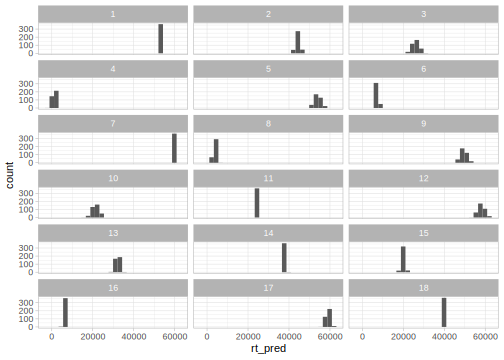
\includegraphics{bookdown_files/figure-latex/priorpred-simple-1.pdf}
\caption{\label{fig:priorpred-simple}Eighteen samples from the prior predictive distribution of the model defined in section \ref{sec:simplenormal}.}
\end{figure}

The prior predictive distribution in Figure \ref{fig:priorpred-simple} shows prior data sets that are not realistic: Besides the fact that the data sets show that response times distributions are symmetrical--and we know that they are generally right-skewed--some data sets present response times that are unrealistically long. Worse yet, if we inspect enough samples from the prior predicted data, it will become clear that a few data sets have negative response time values.

We can also look at the distribution of summary statistics in the prior predictive data. Even if we don't know beforehand what the data should look like, it's very likely that we have some expectations for possible mean, minimum, or maximum values. For example, in the button-pressing example, it seems reasonable to assume that average response times are between 200-600 ms; response times are very unlikely to be below 50 ms (given the delays in keyboards), and even long lapses of attention won't be greater than a couple of seconds.\footnote{We'll see later how to generate prior predictive distributions of statistics such as mean, minimum, or maximum value in section \ref{sec:lognormal} using \texttt{brms} and \texttt{pp\_check}.} This distribution of summary statistics is shown in Figure \ref{fig:priorpred-stats}.



\begin{figure}
\centering
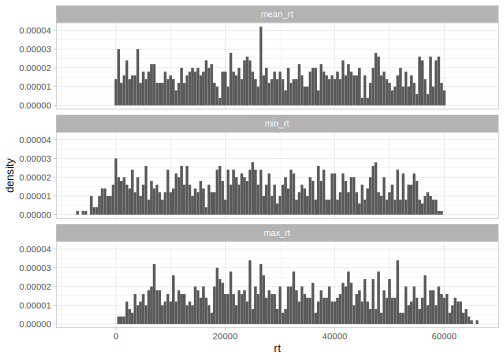
\includegraphics{bookdown_files/figure-latex/priorpred-stats-1.pdf}
\caption{\label{fig:priorpred-stats}Prior predictive distribution of mean, minimum, and maximum value of the button-pressing model defined in section \ref{sec:simplenormal}.}
\end{figure}

Figure \ref{fig:priorpred-stats} shows that we used much less prior information than what we could have: Our priors were encoding the information that any mean between 0 and 60000 ms is equally likely. It seems clear that a value close to 0 or to 60000 ms would be extremely surprising. This wide range of mean values occurs because of the uniform prior on \(\mu\). Similarly, maximum values are quite ``uniform'', spanning a much wider range than what one would expect. Finally, in the distribution of minimum values, negative response times occur. This might seem surprising (our prior for \(\mu\) excluded negative values), but the reason that negative values appear is that the prior is interpreted together with the likelihood (Gelman, Simpson, and Betancourt \protect\hyperlink{ref-gelmanPriorCanOften2017}{2017}), and the likelihood is a normal distribution, which will allow for negative samples even if the location parameter \(\mu\) has a positive value.

To summarize the above discussion, the priors used in the example are clearly not very realistic given what we know about response times for such a button pressing task. This raises the question: what priors should we have chosen? In the next section, we consider this question.

\hypertarget{sec:sensitivity}{%
\section{The influence of priors: sensitivity analysis}\label{sec:sensitivity}}

For most cases that we will encounter in this book, there are four main classes of priors that we can choose from. In the Bayesian community, there is no fixed nomenclature for classifying different kinds of priors. For this book, we have chosen specific names for each type of prior, but this is just a convention that we follow for consistency. There are also other classes of prior that we do not discuss in this book. An example is improper priors such as \(\mathit{Uniform}(-\infty,+\infty)\), which are not proper probability distributions because the area under the curve does not sum to 1.

When thinking about priors, the reader should not get hung up on what precisely the name is for a particular type of prior; they should rather focus on what that prior means in the context of the research problem.

\hypertarget{flat-uninformative-priors}{%
\subsection{Flat, uninformative priors}\label{flat-uninformative-priors}}

One option is to choose priors that are as uninformative as possible. The idea behind this approach is to let the data ``speak for itself'' and to not bias the statistical inference with ``subjective'' priors. There are several issues with this approach: First, the prior is as subjective as the likelihood, and in fact, different choices of likelihood might have a much stronger impact on the posterior than different choices of priors. Second, uninformative priors are in general unrealistic because they give equal weight to all values within the support of the prior distribution, ignoring the fact that usually there is some minimal information about the parameters of interest. Usually, at the very least, the order of magnitude is known (response times will be in milliseconds and not days, EEG signals some microvolts and not volts, etc.). Third, uninformative priors make the sampling slower and might lead to convergence problems. Unless there is a large amount of data, it would be wise to avoid such priors. Fourth, it is not always clear which parametrization of a given distribution the flat priors should be assigned to. For example, the Normal distribution is sometimes defined based on its standard deviation (\(\sigma\)), variance (\(\sigma^2\)), or precision (\(1/\sigma^2\)): a flat prior for the standard deviation is not flat for the precision of the distribution. Although it is sometimes possible to find an uninformative prior that is uninvariant under a change of parameters (also called Jeffreys priors; Jaynes \protect\hyperlink{ref-jaynes2003probability}{2003}, sec. 6.15; Jeffreys \protect\hyperlink{ref-jeffreys1939theory}{1939}, Chapter 3), this is not always the case. Finally, if Bayes factors need to be computed, uninformative priors can lead to very misleading conclusions (chapter \ref{ch:bf}).

In the button-pressing example discussed in this chapter, an example of a flat, uninformative prior would be \(\mu \sim \mathit{Uniform}(-10^{20},10^{20})\). On the millisecond scale, this is a very strange prior to use for a parameter representing mean button-pressing time: it allows for impossibly large positive values, and it also allows negative button-pressing times, which is of course impossible. It is technically possible to use such a prior, but it wouldn't make much sense.

\hypertarget{regularizing-priors}{%
\subsection{Regularizing priors}\label{regularizing-priors}}

If there does not exist much prior information (and if this information cannot be worked out through reasoning about the problem), and there is enough data (what ``enough'' means here will presently become clear when we look at specific examples), it is fine to use \emph{regularizing priors}. These are priors that down-weight extreme values (that is, they provide regularization), they are usually not very informative, and mostly let the likelihood dominate in determining the posteriors. These priors are theory-neutral; that is, they usually do not bias the parameters to values supported by any prior belief or theory. The idea behind this type of prior is to help to stabilize computation. These priors are sometimes called \emph{weakly informative} or \emph{mildly informative} priors in the Bayesian literature. For many applications, they perform well, but discussed in chapter \ref{ch:bf}, they tend to be problematic if Bayes factors need to be computed.

In the button-pressing example, an example of a regularizing prior would be \(\mu \sim \mathit{Normal}_{+}(0,1000)\). This is a Normal distribution prior truncated at 0 ms, and allows a relatively constrained range of positive values for button-pressing times (roughly, up to 2000 ms or so). This is a regularizing prior because it rules out negative button-pressing times and down-weights extremely values over 2000 ms.

\hypertarget{principled-priors}{%
\subsection{Principled priors}\label{principled-priors}}

The idea here is to have priors that encode all (or most of) the theory-neutral information that the researcher has. Since one generally knows what one's data do and do not look like, it is possible to build priors that truly reflect the properties of potential data sets, using prior predictive checks. In this book, many examples of this class of priors will come up.

In the button-pressing data, an example of a principled prior would be \(\mu \sim \mathit{Normal}_{+}(250,100)\). This prior is not overly restrictive, but represents a guess about plausible button-pressing times. Prior predictive checks using principled priors should produce realistic distributions of the dependent variable.

\hypertarget{informative-priors}{%
\subsection{Informative priors}\label{informative-priors}}

There are cases where a lot of prior knowledge exists, and not much data. In general, unless there are \emph{very} good reasons for having informative priors, it is not a good idea to let the priors to have too much influence on the posterior. An example where informative priors would be important is when investigating a language-impaired population from which we can't get many subjects, but a lot of previously published papers exist on the research topic.

In the button-pressing data, an informative prior could be based on a meta-analysis of previously published or existing data, or the result of prior elicitation from an expert (or multiple experts) on the topic under investigation. An example of an informative prior would be \(\mu \sim \mathit{Normal}_{+}(200,20)\). This prior will have some influence on the posterior for \(\mu\), especially when one has relatively sparse data.

These four options constitute a continuum. The uniform prior from the last model (section \ref{sec:simplenormal}) falls between flat, uninformative and regularizing priors. In practical data analysis situations, we are mostly going to choose priors that fall between regularizing and principled. Informative priors, in the sense defined above, will be used only relatively rarely; but they become more important to consider when doing Bayes factor analyses (chapter \ref{ch:bf}).

\hypertarget{sec:revisit}{%
\section{Revisiting the button-pressing example with different priors}\label{sec:revisit}}

What would happen if even wider priors were used for the model defined previously (in section \ref{sec:simplenormal})? Suppose that every mean between \(-10^{10}\) and \(10^{10}\) ms is assumed to be equally likely. This prior is clearly unrealistic and actually makes no sense at all: we are not expecting negative response times. Regarding the standard deviation, one could assume that any value between \(0\) and \(10^{10}\) is equally likely. The likelihood remains unchanged. As before, \texttt{brms} will return a warning; ignore this warning for now.

\begin{equation}
\begin{aligned}
\mu &\sim \mathit{Uniform}(-10^{10}, 10^{10}) \\
\sigma &\sim \mathit{Uniform}(0,  10^{10}) 
\end{aligned}
\label{eq:rtpriorsflat}
\end{equation}

\begin{Shaded}
\begin{Highlighting}[]
\CommentTok{# We fit the model with the default setting of the sampler:}
\CommentTok{# 4 chains, 2000 iterations with half of them as warmup.}
\NormalTok{fit_press_unif <-}\StringTok{ }\KeywordTok{brm}\NormalTok{(rt }\OperatorTok{~}\StringTok{ }\DecValTok{1}\NormalTok{,}
  \DataTypeTok{data =}\NormalTok{ df_spacebar,}
  \DataTypeTok{family =} \KeywordTok{gaussian}\NormalTok{(),}
  \DataTypeTok{prior =} \KeywordTok{c}\NormalTok{(}
    \KeywordTok{prior}\NormalTok{(}\KeywordTok{uniform}\NormalTok{(}\OperatorTok{-}\DecValTok{10}\OperatorTok{^}\DecValTok{10}\NormalTok{, }\DecValTok{10}\OperatorTok{^}\DecValTok{10}\NormalTok{), }\DataTypeTok{class =}\NormalTok{ Intercept),}
    \KeywordTok{prior}\NormalTok{(}\KeywordTok{uniform}\NormalTok{(}\DecValTok{0}\NormalTok{, }\DecValTok{10}\OperatorTok{^}\DecValTok{10}\NormalTok{), }\DataTypeTok{class =}\NormalTok{ sigma)}
\NormalTok{  )}
\NormalTok{)}
\end{Highlighting}
\end{Shaded}

\begin{verbatim}
## Warning: It appears as if you have specified an upper bounded prior on a parameter that has no natural upper bound.
## If this is really what you want, please specify argument 'ub' of 'set_prior' appropriately.
## Warning occurred for prior 
## sigma ~ uniform(0, 10^10)
\end{verbatim}

Even with these extremely unrealistic priors, the output of the model is virtually identical to the previous one (see Figure \ref{fig:postcomp}).

\begin{Shaded}
\begin{Highlighting}[]
\NormalTok{fit_press_unif}
\end{Highlighting}
\end{Shaded}

\begin{verbatim}
## ...
## Population-Level Effects: 
##           Estimate Est.Error l-95% CI u-95% CI Rhat Bulk_ESS Tail_ESS
## Intercept   168.64      1.32   166.15   171.24 1.00     3688     2571
## 
## Family Specific Parameters: 
##       Estimate Est.Error l-95% CI u-95% CI Rhat Bulk_ESS Tail_ESS
## sigma    25.01      0.94    23.27    26.89 1.00     3821     2952
## 
## ...
\end{verbatim}



\begin{figure}
\centering
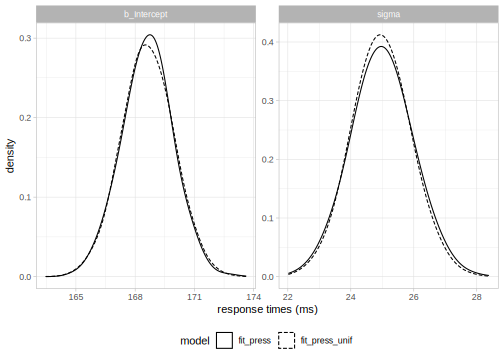
\includegraphics{bookdown_files/figure-latex/postcomp-1.pdf}
\caption{\label{fig:postcomp}Comparison of the posterior distributions from the model with extremely unrealistic priors, \texttt{fit\_press\_unif}, against the previous model with more ``realistically'' bounded uniform distributions (but still not recommended), \texttt{fit\_press}.}
\end{figure}

Next, consider what happens if very informative priors are used. Assume that mean values very close to \(400\) ms are the most likely, and that the standard deviation of the response times is very close to 100 ms. Given that this is a model of button-pressing times, such an informative prior seems wrong---\(200\) ms seems like a more realistic mean button-pressing time, not \(400\) ms. You can check this by doing an experiment yourself and looking at the recorded times; a software like Linger (\url{http://tedlab.mit.edu/~dr/Linger/}) makes it easy to set up such an experiment.

The \(\mathit{Normal}_+\) notation indicates a normal distribution truncated at zero such that only positive values are allowed (Box \ref{thm:truncation} discusses this type of distribution in detail):

\begin{equation}
\begin{aligned}
\mu &\sim \mathit{Normal}(400, 10) \\
\sigma &\sim \mathit{Normal}_+(100, 10) 
\end{aligned}
\label{eq:infrtpriors}
\end{equation}

\begin{Shaded}
\begin{Highlighting}[]
\NormalTok{fit_press_inf <-}\StringTok{ }\KeywordTok{brm}\NormalTok{(rt }\OperatorTok{~}\StringTok{ }\DecValTok{1}\NormalTok{,}
  \DataTypeTok{data =}\NormalTok{ df_spacebar,}
  \DataTypeTok{family =} \KeywordTok{gaussian}\NormalTok{(),}
  \DataTypeTok{prior =} \KeywordTok{c}\NormalTok{(}
    \KeywordTok{prior}\NormalTok{(}\KeywordTok{normal}\NormalTok{(}\DecValTok{400}\NormalTok{, }\DecValTok{10}\NormalTok{), }\DataTypeTok{class =}\NormalTok{ Intercept),}
    \CommentTok{# brms knows that SDs need to be bounded }
    \CommentTok{# to exclude values below zero:}
    \KeywordTok{prior}\NormalTok{(}\KeywordTok{normal}\NormalTok{(}\DecValTok{100}\NormalTok{, }\DecValTok{10}\NormalTok{), }\DataTypeTok{class =}\NormalTok{ sigma)}
\NormalTok{  )}
\NormalTok{)}
\end{Highlighting}
\end{Shaded}

Despite these unrealistic but informative priors, the likelihood mostly dominates and the new posterior means and credible intervals are just a couple of milliseconds away from the previous estimates:

\begin{Shaded}
\begin{Highlighting}[]
\NormalTok{fit_press_inf}
\end{Highlighting}
\end{Shaded}

\begin{verbatim}
## ...
## Population-Level Effects: 
##           Estimate Est.Error l-95% CI u-95% CI Rhat Bulk_ESS Tail_ESS
## Intercept   172.95      1.42   170.28   175.88 1.00     3037     2136
## 
## Family Specific Parameters: 
##       Estimate Est.Error l-95% CI u-95% CI Rhat Bulk_ESS Tail_ESS
## sigma    26.09      1.07    24.06    28.27 1.00     3088     2788
## 
## ...
\end{verbatim}

As a final example of a sensitivity analysis, choose some principled priors. Assuming that we have some prior experience with previous similar experiments, suppose the mean reaction time is expected to be around 200 ms, with a 95\% probability of the mean ranging from 0 to 400 ms. This uncertainty is perhaps unreasonably large, but one might want to allow a bit more uncertainty than one really thinks is reasonable (this kind of conservativity in allowing somewhat more uncertainty is sometimes called Cromwell's rule in Bayesian statistics; see O'Hagan and Forster \protect\hyperlink{ref-kendall2004}{2004}, sec. 3.19). In such a case, one can decide on the prior \(\mathit{Normal}(200, 100)\). Given that the experiment involves only one subject and the task is very simple, one might not expect the residual standard deviation \(\sigma\) to be very large: As an example, one can settle on a location of 50 ms for a truncated normal distribution, but still allow for relatively large uncertainty: \(Normal_{+}(50,50)\).
The prior specifications are summarized below.

\begin{equation}
\begin{aligned}
\mu &\sim \mathit{Normal}(200, 100) \\
\sigma &\sim \mathit{Normal}_+(50, 50) 
\end{aligned}
\end{equation}

Why are these priors principled? The designation ``principled'' here largely depends on our domain knowledge. Chapter \ref{ch:priors} discusses how one can use domain knowledge when specifying priors.

One can achieve a better understanding of what a particular set of priors imply by visualizing the priors graphically, and carrying out prior predictive checks. These steps are skipped here, but these issues will be discussed in detail in chapters \ref{ch:priors} and \ref{ch:workflow}. These chapters will give more detailed information about choosing priors and on developing a principled workflow for Bayesian data analysis.

\begin{Shaded}
\begin{Highlighting}[]
\NormalTok{fit_press_reg <-}\StringTok{ }\KeywordTok{brm}\NormalTok{(rt }\OperatorTok{~}\StringTok{ }\DecValTok{1}\NormalTok{,}
  \DataTypeTok{data =}\NormalTok{ df_spacebar,}
  \DataTypeTok{family =} \KeywordTok{gaussian}\NormalTok{(),}
  \DataTypeTok{prior =} \KeywordTok{c}\NormalTok{(}
    \KeywordTok{prior}\NormalTok{(}\KeywordTok{normal}\NormalTok{(}\DecValTok{200}\NormalTok{, }\DecValTok{100}\NormalTok{), }\DataTypeTok{class =}\NormalTok{ Intercept),}
    \KeywordTok{prior}\NormalTok{(}\KeywordTok{normal}\NormalTok{(}\DecValTok{50}\NormalTok{, }\DecValTok{50}\NormalTok{), }\DataTypeTok{class =}\NormalTok{ sigma)}
\NormalTok{  )}
\NormalTok{)}
\end{Highlighting}
\end{Shaded}

The new estimates are virtually the same as before:

\begin{Shaded}
\begin{Highlighting}[]
\NormalTok{fit_press_reg}
\end{Highlighting}
\end{Shaded}

\begin{verbatim}
## ...
## Population-Level Effects: 
##           Estimate Est.Error l-95% CI u-95% CI Rhat Bulk_ESS Tail_ESS
## Intercept   168.63      1.29   166.01   171.15 1.00     2840     2376
## 
## Family Specific Parameters: 
##       Estimate Est.Error l-95% CI u-95% CI Rhat Bulk_ESS Tail_ESS
## sigma    25.00      0.93    23.30    26.86 1.00     3288     2745
## 
## ...
\end{verbatim}

The above examples of using different priors should not be misunderstood to mean that priors never matter. When there is enough data, the likelihood will dominate in determining the posterior distributions. What constitutes ``enough'' data is also a function of the complexity of the model; as a general rule, more complex models require more data. For example, parameters that represent group-level (also known as random) effects in hierarchical (or mixed) models, require much more data than population-level (also known as fixed) effects. This means that, in general, priors will have a greater impact on the estimation of group-level parameters than of population-level parameters. An important observation here is that in general the posterior uncertainty of the population-level parameters will also be affected by the uncertainty in the group-level parameters. In other words, if the posterior estimates for the random effects have wide uncertainty, then the posteriors of the fixed effects will be affected by that uncertainty. This will be verified using simulation later in the book (chapter \ref{ch:workflow}).

Even in cases where there is enough data and the likelihood dominates in determining the posteriors, regularizing, principled priors (i.e., priors that are more consistent with our a priori beliefs about the data) will in general speed-up model convergence.

In order to determine the extent to which the posterior is influenced by the priors, it is a good practice to carry out a sensitivity analysis: try different priors and either verify that the posterior doesn't change drastically, or report how the posterior is affected by some specific priors (for examples from psycholinguistics, see Vasishth et al. \protect\hyperlink{ref-VasishthetalPLoSOne2013}{2013}; Vasishth and Engelmann \protect\hyperlink{ref-VasishthEngelmann2022}{2022}). Chapter \ref{ch:bf} will demonstrate that sensitivity analysis becomes crucial for reporting Bayes factors; even in cases where the choice of priors does not affect the posterior distribution, it generally affects the Bayes factor.

\hypertarget{sec:ppd}{%
\section{Posterior predictive distribution}\label{sec:ppd}}

The prior predictive distribution is a collection of data sets generated from the model (the likelihood and the priors). Having obtained the posterior distributions of the parameters after taking into account the data, the posterior distributions can be used to generate future data from the model. In other words, given the posterior distributions of the parameters of the model, the posterior predictive distribution gives us some indication of what future data might look like, given the data and model of course.

Once the posterior distributions \(p(\boldsymbol{\Theta}\mid \boldsymbol{y})\) are available, the predictions based on these distributions, by integrating out the parameters:

\begin{equation}
p(\boldsymbol{y_{pred}}\mid \boldsymbol{y} ) = \int_{\boldsymbol{\Theta}} p(\boldsymbol{y_{pred}}, \boldsymbol{\Theta}\mid \boldsymbol{y})\, d\boldsymbol{\Theta}= \int_{\boldsymbol{\Theta}} 
p(\boldsymbol{y_{pred}}\mid \boldsymbol{\Theta},\boldsymbol{y})p(\boldsymbol{\Theta}\mid \boldsymbol{y})\, d\boldsymbol{\Theta}
\end{equation}

Assuming that past and future observations are conditionally independent given \(\boldsymbol{\Theta}\), i.e., \(p(\boldsymbol{y_{pred}}\mid \boldsymbol{\Theta},\boldsymbol{y})= p(\boldsymbol{y_{pred}}\mid \boldsymbol{\Theta})\), the above equation can be written as:

\begin{equation}
p(\boldsymbol{y_{pred}}\mid \boldsymbol{y} )=\int_{\boldsymbol{\Theta}} p(\boldsymbol{y_{pred}}\mid \boldsymbol{\Theta}) p(\boldsymbol{\Theta}\mid \boldsymbol{y})\, d\boldsymbol{\Theta}
\label{eq:postpp}
\end{equation}

In Equation \eqref{eq:postpp}, we are conditioning \(\boldsymbol{y_{pred}}\) only on \(\boldsymbol{y}\), we do not condition on what we don't know (\(\boldsymbol{\Theta}\)); the unknown parameters have been integrated out. This posterior predictive distribution has important differences from the frequentist approach. The latter gives only a predictive distribution of \(\boldsymbol{y_{pred}}\) given the maximum likelihood estimate of \(\boldsymbol{\Theta}\) (a point value). As with the prior predictive distribution, the integration can be carried out computationally by generating samples from the posterior predictive distribution. The same function that we created before, \texttt{normal\_predictive\_distribution}, can be used here. The only difference is that instead of sampling \texttt{mu} and \texttt{sigma} from the priors, the samples come from the posterior.

\begin{Shaded}
\begin{Highlighting}[]
\NormalTok{N_obs <-}\StringTok{ }\KeywordTok{nrow}\NormalTok{(df_spacebar)}
\NormalTok{mu_samples <-}\StringTok{ }\KeywordTok{as_draws_df}\NormalTok{(fit_press)}\OperatorTok{$}\NormalTok{b_Intercept}
\NormalTok{sigma_samples <-}\StringTok{ }\KeywordTok{as_draws_df}\NormalTok{(fit_press)}\OperatorTok{$}\NormalTok{sigma}
\KeywordTok{normal_predictive_distribution}\NormalTok{(}
  \DataTypeTok{mu_samples =}\NormalTok{ mu_samples,}
  \DataTypeTok{sigma_samples =}\NormalTok{ sigma_samples,}
  \DataTypeTok{N_obs =}\NormalTok{ N_obs}
\NormalTok{)}
\end{Highlighting}
\end{Shaded}

\begin{verbatim}
## # A tibble: 1,444,000 x 3
##    iter trialn rt_pred
##   <dbl>  <int>   <dbl>
## 1     1      1    138.
## 2     1      2    135.
## 3     1      3    175.
## # ... with 1,443,997 more rows
\end{verbatim}

The \texttt{brms} function \texttt{posterior\_predict()} is a convenient function that delivers samples from the posterior predictive distribution. Using the command \texttt{posterior\_predict(fit\_press)} yields the predicted response times in a matrix, with the samples as rows and the observations (data-points) as columns. (Bear in mind that if a model is fit with \texttt{sample\_prior\ =\ "only"}, the dependent variable is ignored and \texttt{posterior\_predict} will yield samples from the prior predictive distribution).

The posterior predictive distribution can be used to examine the ``descriptive adequacy'' of the model under consideration (Gelman et al. \protect\hyperlink{ref-Gelman14}{2014}, Chapter 6; Shiffrin et al. \protect\hyperlink{ref-shiffrinSurveyModelEvaluation2008}{2008}). Examining the posterior predictive distribution to establish descriptive adequacy is called posterior predictive checks. The goal here is to establish that the posterior predictive data look more or less similar to the observed data. Achieving descriptive adequacy means that the current data could have been generated by the model. Although passing a test of descriptive adequacy is not strong evidence in favor of a model, a major failure in descriptive adequacy can be interpreted as strong evidence against a model (Shiffrin et al. \protect\hyperlink{ref-shiffrinSurveyModelEvaluation2008}{2008}).
For this reason, comparing the descriptive adequacy of different models is not enough to differentiate between their relative performance. When doing model comparison, it is important to consider the criteria that Roberts and Pashler (\protect\hyperlink{ref-rp}{2000}) define. Although Roberts and Pashler (\protect\hyperlink{ref-rp}{2000}) are more interested in process models and not necessarily Bayesian models, their criteria are important for any kind of model comparison. Their main point is that it is not enough to have a good fit to the data for a model to be convincing. One should check that the range of predictions that the model makes is reasonably constrained; if a model can capture any possible outcome, then the model fit to a particular data set is not so informative. Thus, although posterior predictive checking is important, it is only a sanity check to assess whether the model behavior is reasonable.

In many cases, one can simply use the plot functions from \texttt{brms} (that act as wrappers for \texttt{bayesplot} functions). For example, the plotting function \texttt{pp\_check} takes as arguments the model, the number of predicted data sets, and the type of visualization, and it can display different visualizations of posterior predictive checks. In these type of plots, the observed data are plotted as \(y\) and predicted data as \(y_{rep}\). Below, we use \texttt{pp\_check} to investigate how well the observed distribution of response times fit our model based on some number (11 and 100) of samples of the posterior predictive distributions (that is, simulated data sets) ; see Figures \ref{fig:normalppc} and \ref{fig:normalppc2}.



\begin{Shaded}
\begin{Highlighting}[]
\KeywordTok{pp_check}\NormalTok{(fit_press, }\DataTypeTok{ndraws =} \DecValTok{11}\NormalTok{, }\DataTypeTok{type =} \StringTok{"hist"}\NormalTok{)}
\end{Highlighting}
\end{Shaded}

\begin{figure}
\centering
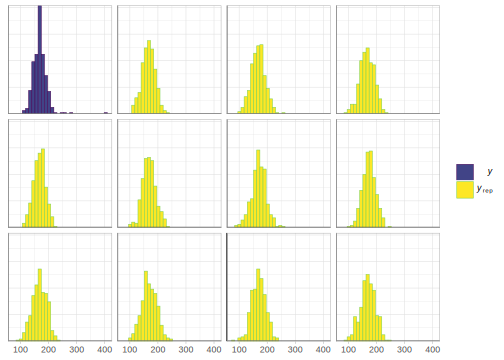
\includegraphics{bookdown_files/figure-latex/normalppc-1.pdf}
\caption{\label{fig:normalppc}Histograms of eleven samples from the posterior predictive distribution of the model \texttt{fit\_press} (\(y_{rep}\)).}
\end{figure}



\begin{Shaded}
\begin{Highlighting}[]
\KeywordTok{pp_check}\NormalTok{(fit_press, }\DataTypeTok{ndraws =} \DecValTok{100}\NormalTok{, }\DataTypeTok{type =} \StringTok{"dens_overlay"}\NormalTok{)}
\end{Highlighting}
\end{Shaded}

\begin{figure}
\centering
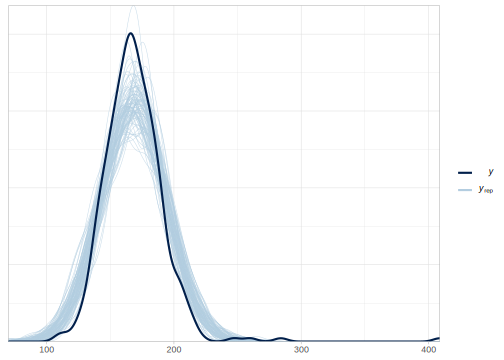
\includegraphics{bookdown_files/figure-latex/normalppc2-1.pdf}
\caption{\label{fig:normalppc2}Posterior predictive check that shows the fit of the model \texttt{fit\_press} in comparison to data sets from the posterior predictive distribution using an overlay of density plots.}
\end{figure}

The data is slightly skewed and has no values smaller than 100 ms, but the predictive distributions are centered and symmetrical; see figures \ref{fig:normalppc} and \ref{fig:normalppc2}. This posterior predictive check shows a slight mismatch between the observed and predicted data. Can we build a better model? We'll come back to this issue in the next section.

\hypertarget{comparing-different-likelihoods}{%
\subsection{Comparing different likelihoods}\label{comparing-different-likelihoods}}

Response times are not usually normally distributed. A more realistic distribution is the log-normal. A random variable (such as time) that is log-normally distributed takes only positive real values and is right-skewed. Although other distributions can also produce data with such properties, the log-normal will turn out to be a pretty reasonable distribution for response times.

\hypertarget{sec:lnfirst}{%
\subsection{The log-normal likelihood}\label{sec:lnfirst}}

If \(\boldsymbol{y}\) is log-normally distributed, this means that \(\log(\boldsymbol{y})\) is normally distributed.\footnote{More precisely, \(\log_e(\boldsymbol{y})\) or \(\ln(\boldsymbol{y})\), but we'll write it as just \(log()\).} The log-normal distribution is also defined using the parameters location, \(\mu\), and scale, \(\sigma\), but these are on the log ms scale; they correspond to the mean and standard deviation of the logarithm of the data \(\boldsymbol{y}\), \(\log(\boldsymbol{y})\), which will be normally distributed. Thus, when we model some data \(\boldsymbol{y}\) using the log-normal likelihood, the parameters \(\mu\) and \(\sigma\) are on a different scale than the data \(\boldsymbol{y}\). Equation \eqref{eq:lognormalequations} shows the relationship between the log-normal and the normal.

\begin{equation}
\begin{aligned}
\log(\boldsymbol{y}) &\sim \mathit{Normal}( \mu, \sigma)\\
\boldsymbol{y} &\sim \mathit{LogNormal}( \mu, \sigma) 
\end{aligned}
\label{eq:lognormalequations}
\end{equation}

We can obtain samples from the log-normal distribution, using the normal distribution by first setting an auxiliary variable, \(z\), so that \(z = \log(y)\). This means that \(z \sim \mathit{Normal}(\mu, \sigma)\).
Then we can just use \(exp(z)\) as samples from the \(\mathit{LogNormal}(\mu, \sigma)\), since \(\exp(z) =\exp(\log(y)) = y\). The code below produces Figure \ref{fig:logndemo}.

\begin{Shaded}
\begin{Highlighting}[]
\NormalTok{mu <-}\StringTok{ }\DecValTok{6}
\NormalTok{sigma <-}\StringTok{ }\FloatTok{0.5}
\NormalTok{N <-}\StringTok{ }\DecValTok{500000}
\CommentTok{# Generate N random samples from a log-normal distribution}
\NormalTok{sl <-}\StringTok{ }\KeywordTok{rlnorm}\NormalTok{(N, mu, sigma)}
\KeywordTok{ggplot}\NormalTok{(}\KeywordTok{tibble}\NormalTok{(}\DataTypeTok{samples =}\NormalTok{ sl), }\KeywordTok{aes}\NormalTok{(samples)) }\OperatorTok{+}
\StringTok{  }\KeywordTok{geom_histogram}\NormalTok{(}\KeywordTok{aes}\NormalTok{(}\DataTypeTok{y =}\NormalTok{ ..density..), }\DataTypeTok{binwidth =} \DecValTok{50}\NormalTok{) }\OperatorTok{+}
\StringTok{  }\KeywordTok{ggtitle}\NormalTok{(}\StringTok{"Log-normal distribution}\CharTok{\textbackslash{}n}\StringTok{"}\NormalTok{) }\OperatorTok{+}
\StringTok{  }\KeywordTok{coord_cartesian}\NormalTok{(}\DataTypeTok{xlim =} \KeywordTok{c}\NormalTok{(}\DecValTok{0}\NormalTok{, }\DecValTok{2000}\NormalTok{))}
\CommentTok{# Generate N random samples from a normal distribution,}
\CommentTok{# and then exponentiate them}
\NormalTok{sn <-}\StringTok{ }\KeywordTok{exp}\NormalTok{(}\KeywordTok{rnorm}\NormalTok{(N, mu, sigma))}
\KeywordTok{ggplot}\NormalTok{(}\KeywordTok{tibble}\NormalTok{(}\DataTypeTok{samples =}\NormalTok{ sn), }\KeywordTok{aes}\NormalTok{(samples)) }\OperatorTok{+}
\StringTok{  }\KeywordTok{geom_histogram}\NormalTok{(}\KeywordTok{aes}\NormalTok{(}\DataTypeTok{y =}\NormalTok{ ..density..), }\DataTypeTok{binwidth =} \DecValTok{50}\NormalTok{) }\OperatorTok{+}
\StringTok{  }\KeywordTok{ggtitle}\NormalTok{(}\StringTok{"Exponentiated samples from}\CharTok{\textbackslash{}n}\StringTok{a normal distribution"}\NormalTok{) }\OperatorTok{+}
\StringTok{  }\KeywordTok{coord_cartesian}\NormalTok{(}\DataTypeTok{xlim =} \KeywordTok{c}\NormalTok{(}\DecValTok{0}\NormalTok{, }\DecValTok{2000}\NormalTok{))}
\end{Highlighting}
\end{Shaded}

\begin{figure}
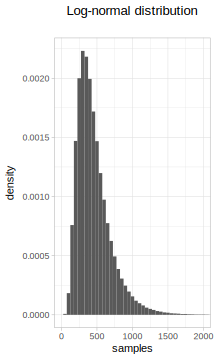
\includegraphics[width=0.48\linewidth]{bookdown_files/figure-latex/logndemo-1} 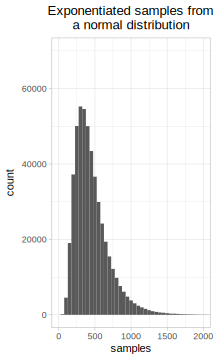
\includegraphics[width=0.48\linewidth]{bookdown_files/figure-latex/logndemo-2} \caption{Two log-normal distributions with the same parameters generated by either generating samples from a log-normal distribution or exponentiating samples from a normal distribution.}\label{fig:logndemo}
\end{figure}

\hypertarget{sec:lognormal}{%
\subsection{Re-fitting a single subject pressing a button repeatedly with a log-normal likelihood}\label{sec:lognormal}}

If we assume that response times are log-normally distributed, we'll need to change our likelihood function as follows:

\begin{equation}
rt_n \sim \mathit{LogNormal}(\mu,\sigma)
\end{equation}

But now the scale of our priors needs to change! We'll start with uniform priors for ease of exposition, even though, as we mentioned earlier, these are not really appropriate here. (Below, we show these uniform priors, as well as examples of more realistic priors.)

\begin{equation}
\begin{aligned}
\mu &\sim \mathit{Uniform}(0, 11) \\
\sigma &\sim \mathit{Uniform}(0, 1) \\
\end{aligned}
\label{eq:logpriorsunif}
\end{equation}

Because the parameters are on a different scale than the dependent variable, their interpretation changes and it is more complex than if we were dealing with a linear model that assumes a normal likelihood (location and scale do not coincide with the mean and standard deviation of the log-normal):

\begin{itemize}
\tightlist
\item
  \emph{The location, \(\mu\)}: In our previous linear model, \(\mu\) represented the mean (in a normal distribution, the mean happens to be identical to the median and the mode). But now, the mean needs to be calculated in the following way, \(\exp(\mu +\sigma ^{2}/2)\). In other words, in the log-normal, the mean is dependent on both \(\mu\) and \(\sigma\). The median is just \(\exp(\mu)\). Notice that the prior of \(\mu\) is not on the milliseconds scale, but rather on the log milliseconds scale.
\item
  \emph{The scale, \(\sigma\)}: This is the standard deviation of the normal distribution of \(\log(\boldsymbol{y})\). The standard deviation of a log-normal distribution with \emph{location} \(\mu\) and \emph{scale} \(\sigma\) will be \(\exp(\mu +\sigma ^{2}/2)\times \sqrt{\exp(\sigma^2)- 1}\). Unlike the normal distribution, the spread of the log-normal distribution depends on both \(\mu\) and \(\sigma\).
\end{itemize}

To understand the meaning of our priors on the millisecond scale, we need to take into account both the priors and the likelihood. We can do this by generating a prior predictive distribution. We can just exponentiate the samples produced by \texttt{normal\_predictive\_distribution()} (or, alternatively, we could have edited the function and replaced \texttt{rnorm} with \texttt{rlnorm}).

\begin{Shaded}
\begin{Highlighting}[]
\NormalTok{N_samples <-}\StringTok{ }\DecValTok{1000}
\NormalTok{N_obs <-}\StringTok{ }\KeywordTok{nrow}\NormalTok{(df_spacebar)}
\NormalTok{mu_samples <-}\StringTok{ }\KeywordTok{runif}\NormalTok{(N_samples, }\DecValTok{0}\NormalTok{, }\DecValTok{11}\NormalTok{)}
\NormalTok{sigma_samples <-}\StringTok{ }\KeywordTok{runif}\NormalTok{(N_samples, }\DecValTok{0}\NormalTok{, }\DecValTok{1}\NormalTok{)}
\NormalTok{prior_pred_ln <-}\StringTok{ }\KeywordTok{normal_predictive_distribution}\NormalTok{(}
  \DataTypeTok{mu_samples =}\NormalTok{ mu_samples,}
  \DataTypeTok{sigma_samples =}\NormalTok{ sigma_samples,}
  \DataTypeTok{N_obs =}\NormalTok{ N_obs}
\NormalTok{) }\OperatorTok
\StringTok{  }\KeywordTok{mutate}\NormalTok{(}\DataTypeTok{rt_pred =} \KeywordTok{exp}\NormalTok{(rt_pred))}
\end{Highlighting}
\end{Shaded}

Next, plot the distribution of some representative statistics; see Figure \ref{fig:priorpredlogunif}.



\begin{figure}
\centering
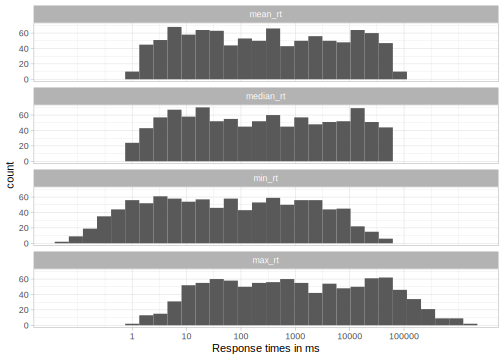
\includegraphics{bookdown_files/figure-latex/priorpredlogunif-1.pdf}
\caption{\label{fig:priorpredlogunif}The prior predictive distribution of the mean, median, minimum, and maximum value of the log-normal model with priors defined in Equation \eqref{eq:logpriorsunif}, that is \(\mu \sim \mathit{Uniform}(0, 11)\) and \(\sigma \sim \mathit{Uniform}(0, 1)\). The x-axis is log-transformed.}
\end{figure}

We cannot generate negative values any more, since \(\exp(\)any finite real number\() > 0\). These priors might work in the sense that the model might converge; but it would be better to have regularizing priors for the model. An example is the following priors:

\begin{equation}
\begin{aligned}
\mu &\sim \mathit{Normal}(6, 1.5) \\
\sigma &\sim \mathit{Normal}_+(0, 1) \\
\end{aligned}
\label{eq:logpriorsnorm}
\end{equation}

The prior for \(\sigma\) here is a truncated distribution, and although its location is zero, this is not its mean. We can calculate its approximate mean from a large number of random samples of the prior distribution using the function \texttt{rtnorm} from the package \texttt{extraDistr}. In this function, we have to set the parameter \texttt{a\ =\ 0} to express the fact that the normal distribution is truncated from the left at 0.

\begin{Shaded}
\begin{Highlighting}[]
\KeywordTok{mean}\NormalTok{(}\KeywordTok{rtnorm}\NormalTok{(}\DecValTok{100000}\NormalTok{, }\DecValTok{0}\NormalTok{, }\DecValTok{1}\NormalTok{, }\DataTypeTok{a =} \DecValTok{0}\NormalTok{))}
\end{Highlighting}
\end{Shaded}

\begin{verbatim}
## [1] 0.797
\end{verbatim}

Even before generating the prior predictive distributions, we can calculate the values within which we are 95\% sure that the expected median of the observations will lie. We do this by looking at what happens at two standard deviations away from the mean of the prior, \(\mu\), that is \(6 - 2\times 1.5\) and \(6 + 2\times 1.5\), and exponentiating these values:

\begin{Shaded}
\begin{Highlighting}[]
\KeywordTok{c}\NormalTok{(}
  \DataTypeTok{lower =} \KeywordTok{exp}\NormalTok{(}\DecValTok{6} \OperatorTok{-}\StringTok{ }\DecValTok{2} \OperatorTok{*}\StringTok{ }\FloatTok{1.5}\NormalTok{),}
  \DataTypeTok{higher =} \KeywordTok{exp}\NormalTok{(}\DecValTok{6} \OperatorTok{+}\StringTok{ }\DecValTok{2} \OperatorTok{*}\StringTok{ }\FloatTok{1.5}\NormalTok{)}
\NormalTok{)}
\end{Highlighting}
\end{Shaded}

\begin{verbatim}
##  lower higher 
##   20.1 8103.1
\end{verbatim}

This means that our prior for \(\mu\) is still not too informative (these are medians; the actual values generated by the log-normal distribution can be much more spread out). We can now plot the distribution of some representative statistics of the prior predictive distributions.
We use \texttt{brms} to sample from the priors ignoring the \texttt{rt} data, by setting \texttt{sample\_prior\ =\ "only"}.

If we want to use \texttt{brms} to generate prior predictive data in this manner before collecting the data, we do need to have \emph{some} simulated values that represent the vector of dependent variables, \texttt{rt}. Because these values will be plotted alongside with the prior predictive distributions in \texttt{pp\_check}, they can be used to compare the prior predictive data with the simulated \texttt{rt} vector. In this case, as an example, we choose \(\mathit{Uniform}(0,10000)\) to generate the simulated \texttt{rt} vector. We need to specify that the family is \texttt{lognormal()}. In our first example, we had used the family \texttt{gaussian()}.

\begin{Shaded}
\begin{Highlighting}[]
\NormalTok{df_spacebar_ref <-}\StringTok{ }\NormalTok{df_spacebar }\OperatorTok
\StringTok{  }\KeywordTok{mutate}\NormalTok{(}\DataTypeTok{rt =} \KeywordTok{runif}\NormalTok{(}\KeywordTok{n}\NormalTok{(), }\DecValTok{0}\NormalTok{, }\DecValTok{10000}\NormalTok{))}
\NormalTok{fit_prior_press_ln <-}\StringTok{ }\KeywordTok{brm}\NormalTok{(rt }\OperatorTok{~}\StringTok{ }\DecValTok{1}\NormalTok{,}
  \DataTypeTok{data =}\NormalTok{ df_spacebar_ref,}
  \DataTypeTok{family =} \KeywordTok{lognormal}\NormalTok{(),}
  \DataTypeTok{prior =} \KeywordTok{c}\NormalTok{(}
    \KeywordTok{prior}\NormalTok{(}\KeywordTok{normal}\NormalTok{(}\DecValTok{6}\NormalTok{, }\FloatTok{1.5}\NormalTok{), }\DataTypeTok{class =}\NormalTok{ Intercept),}
    \KeywordTok{prior}\NormalTok{(}\KeywordTok{normal}\NormalTok{(}\DecValTok{0}\NormalTok{, }\DecValTok{1}\NormalTok{), }\DataTypeTok{class =}\NormalTok{ sigma)}
\NormalTok{  ),}
  \DataTypeTok{sample_prior =} \StringTok{"only"}\NormalTok{,}
  \DataTypeTok{control =} \KeywordTok{list}\NormalTok{(}\DataTypeTok{adapt_delta =} \FloatTok{.95}\NormalTok{)}
\NormalTok{)}
\end{Highlighting}
\end{Shaded}

To avoid the warnings, we need to increase the \texttt{adapt\_delta} parameter's default value from 0.8 to 0.95 to simulate the data. Since Stan samples from the prior distributions in the same way that it samples from the posterior distribution, we should not ignore warnings. One should always ensure that the model converged. In that respect, our custom function \texttt{normal\_predictive\_distribution()} defined in \ref{sec:priorpred} has the advantage that, since it just relies on the \texttt{rnorm} function, it will always yield independent samples from the prior distribution and will not experience any convergence problems.

Plot the prior predictive distribution of means with the following code (the figure is not produced here, to conserve space):

\begin{Shaded}
\begin{Highlighting}[]
\KeywordTok{pp_check}\NormalTok{(fit_prior_press_ln, }\DataTypeTok{type =} \StringTok{"stat"}\NormalTok{, }\DataTypeTok{stat =} \StringTok{"mean"}\NormalTok{) }\OperatorTok{+}
\StringTok{  }\KeywordTok{coord_cartesian}\NormalTok{(}\DataTypeTok{xlim =} \KeywordTok{c}\NormalTok{(}\FloatTok{0.001}\NormalTok{, }\DecValTok{300000}\NormalTok{)) }\OperatorTok{+}
\StringTok{  }\KeywordTok{scale_x_continuous}\NormalTok{(}\StringTok{"Response times [ms]"}\NormalTok{,}
    \DataTypeTok{trans =} \StringTok{"log"}\NormalTok{,}
    \DataTypeTok{breaks =} \KeywordTok{c}\NormalTok{(}\FloatTok{0.001}\NormalTok{, }\DecValTok{1}\NormalTok{, }\DecValTok{100}\NormalTok{, }\DecValTok{1000}\NormalTok{, }\DecValTok{10000}\NormalTok{, }\DecValTok{100000}\NormalTok{),}
    \DataTypeTok{labels =} \KeywordTok{c}\NormalTok{(}
      \StringTok{"0.001"}\NormalTok{, }\StringTok{"1"}\NormalTok{, }\StringTok{"100"}\NormalTok{, }\StringTok{"1000"}\NormalTok{, }\StringTok{"10000"}\NormalTok{,}
      \StringTok{"100000"}
\NormalTok{    )}
\NormalTok{  ) }\OperatorTok{+}
\StringTok{  }\KeywordTok{ggtitle}\NormalTok{(}\StringTok{"Prior predictive distribution of means"}\NormalTok{)}
\end{Highlighting}
\end{Shaded}

To plot the distribution of minimum, and maximum values, just replace \texttt{mean} with \texttt{min}, and \texttt{max} respectively. The three statistics are displayed in Figure \ref{fig:priorpredlognorm}.



\begin{figure}
\centering
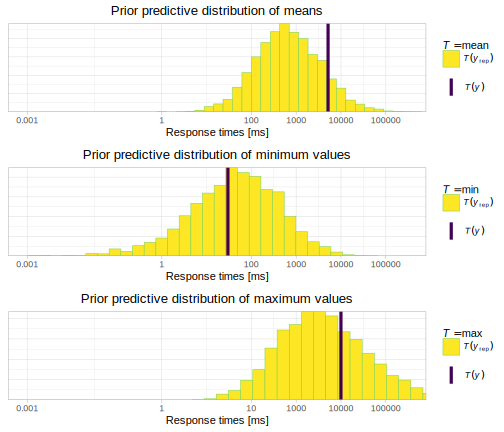
\includegraphics{bookdown_files/figure-latex/priorpredlognorm-1.pdf}
\caption{\label{fig:priorpredlognorm}Prior predictive distribution of mean, maximum, and minimum values of the log-normal model with priors defined in Equation \eqref{eq:logpriorsnorm}. The distributions of mean, minimum, and maximum values of the prior predictive distributions are labeled \(y_{rep}\) and the mean, minimum, and maximum values for the ``reference'' distribution, \(\mathit{Uniform}(0,10000)\), are labeled \(y\). The x-axis is log-transformed.}
\end{figure}

Figure \ref{fig:priorpredlognorm} shows that the priors that we are using are still quite uninformative. The tails of the prior predictive distributions that correspond to our normal priors shown in Figure \ref{fig:priorpredlognorm} are even further to the right, reaching more extreme values than for the prior predictive distributions generated by uniform priors (shown in Figure \ref{fig:priorpredlogunif}). Our new priors are still far from representing our prior knowledge. We could do more iterations of choosing priors and generating prior predictive distributions until we have priors that generate realistic data. However, given that the bulk of the distributions of mean, maximum, minimum values lies roughly in the correct order of magnitude, these priors are going to be acceptable. In general, we can use summary statistics (e.g., mean, median, min, max) to test whether the priors are in a plausible range. We can do this by defining, for the particular research problem we are studying, the extreme data that would be very implausible to ever observe (e.g., reading times at a word larger than one minute) and choosing priors such that such extreme response times occur only very rarely in the prior predictive distribution.

We can fit the model now; recall that both the distribution family and prior change in comparison to our previous example.

\begin{Shaded}
\begin{Highlighting}[]
\NormalTok{fit_press_ln <-}\StringTok{ }\KeywordTok{brm}\NormalTok{(rt }\OperatorTok{~}\StringTok{ }\DecValTok{1}\NormalTok{,}
  \DataTypeTok{data =}\NormalTok{ df_spacebar,}
  \DataTypeTok{family =} \KeywordTok{lognormal}\NormalTok{(),}
  \DataTypeTok{prior =} \KeywordTok{c}\NormalTok{(}
    \KeywordTok{prior}\NormalTok{(}\KeywordTok{normal}\NormalTok{(}\DecValTok{6}\NormalTok{, }\FloatTok{1.5}\NormalTok{), }\DataTypeTok{class =}\NormalTok{ Intercept),}
    \KeywordTok{prior}\NormalTok{(}\KeywordTok{normal}\NormalTok{(}\DecValTok{0}\NormalTok{, }\DecValTok{1}\NormalTok{), }\DataTypeTok{class =}\NormalTok{ sigma)}
\NormalTok{  )}
\NormalTok{)}
\end{Highlighting}
\end{Shaded}

When we look at the summary of the posterior, the parameters are on the log-scale:

\begin{Shaded}
\begin{Highlighting}[]
\NormalTok{fit_press_ln}
\end{Highlighting}
\end{Shaded}

\begin{verbatim}
## ...
## Population-Level Effects: 
##           Estimate Est.Error l-95% CI u-95% CI Rhat Bulk_ESS Tail_ESS
## Intercept     5.12      0.01     5.10     5.13 1.00     3938     2652
## 
## Family Specific Parameters: 
##       Estimate Est.Error l-95% CI u-95% CI Rhat Bulk_ESS Tail_ESS
## sigma     0.13      0.00     0.13     0.14 1.00     2709     2348
## 
## ...
\end{verbatim}

If we want to know how long it takes to press the space bar in milliseconds, we need to transform the \(\mu\) (or \texttt{Intercept} in the model) to milliseconds. Since we know that the median of the log-normal distribution is \(\exp(\mu)\), we do the following to calculate an estimate in milliseconds:

\begin{Shaded}
\begin{Highlighting}[]
\NormalTok{estimate_ms <-}\StringTok{ }\KeywordTok{exp}\NormalTok{(}\KeywordTok{as_draws_df}\NormalTok{(fit_press_ln)}\OperatorTok{$}\NormalTok{b_Intercept)}
\end{Highlighting}
\end{Shaded}

If we want to know the mean and 95\% credible interval of these samples, we do the following:

\begin{Shaded}
\begin{Highlighting}[]
\KeywordTok{c}\NormalTok{(}\DataTypeTok{mean =} \KeywordTok{mean}\NormalTok{(estimate_ms), }\KeywordTok{quantile}\NormalTok{(estimate_ms, }\DataTypeTok{probs =} \KeywordTok{c}\NormalTok{(.}\DecValTok{025}\NormalTok{, }\FloatTok{.975}\NormalTok{)))}
\end{Highlighting}
\end{Shaded}

\begin{verbatim}
##  mean  2.5% 97.5% 
##   167   165   169
\end{verbatim}

We can now check whether our predicted data sets look similar to
the real data set. See Figure \ref{fig:logppc}; compare this with the earlier Figure \ref{fig:normalppc2}.



\begin{Shaded}
\begin{Highlighting}[]
\KeywordTok{pp_check}\NormalTok{(fit_press_ln, }\DataTypeTok{ndraws =} \DecValTok{100}\NormalTok{)}
\end{Highlighting}
\end{Shaded}

\begin{figure}
\centering
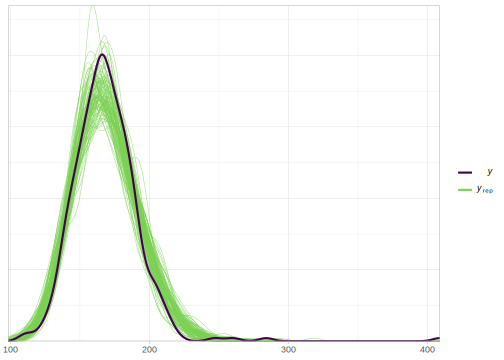
\includegraphics{bookdown_files/figure-latex/logppc-1.pdf}
\caption{\label{fig:logppc}Posterior predictive distribution of \texttt{fit\_noreading\_ln}.}
\end{figure}

We ask: Are the posterior predicted data now more similar to the real data, compared to the case where we had a Normal likelihood?

According to Figure \ref{fig:logppc}, it seems so, but it's not easy to tell.

Another way to examine this would be to look at the distribution of summary statistics. We compare the distribution of representative summary statistics for the data sets generated by different models and compare them to the observed statistics. We suspect that the normal distribution would generate response times that are too fast (since it's symmetrical) and that the log-normal distribution may capture the long tail better than the normal model. Based on our hunch, we compute the distribution of minimum and maximum values for the posterior predictive distributions, and we compare them with the minimum and maximum value respectively in the data. We do this with \texttt{pp\_check}, by using as stat either \texttt{"min"} or \texttt{"max"} for both \texttt{fit\_press}, and \texttt{fit\_press\_ln}; an example is shown below. The plots are shown in Figures \ref{fig:ppcheckmin} and \ref{fig:ppcheckmax}.

\begin{Shaded}
\begin{Highlighting}[]
\KeywordTok{pp_check}\NormalTok{(fit_press, }\DataTypeTok{type =} \StringTok{"stat"}\NormalTok{, }\DataTypeTok{stat =} \StringTok{"min"}\NormalTok{)}
\end{Highlighting}
\end{Shaded}

\begin{figure}
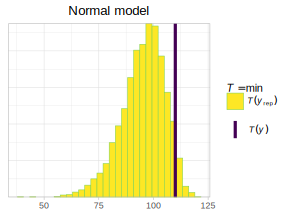
\includegraphics[width=0.45\linewidth]{bookdown_files/figure-latex/ppcheckmin-1} 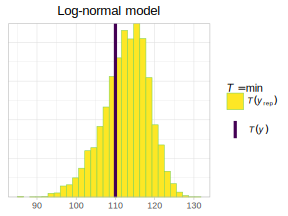
\includegraphics[width=0.45\linewidth]{bookdown_files/figure-latex/ppcheckmin-2} \caption{Distributions of minimum values in a posterior predictive check, using the normal and log-normal probability density functions. The minimum in the data is 110 ms.}\label{fig:ppcheckmin}
\end{figure}

\begin{figure}
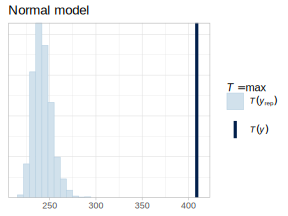
\includegraphics[width=0.45\linewidth]{bookdown_files/figure-latex/ppcheckmax-1} 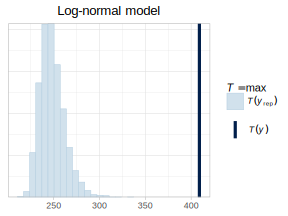
\includegraphics[width=0.45\linewidth]{bookdown_files/figure-latex/ppcheckmax-2} \caption{Distribution of maximum values in a posterior predictive check. The maximum in the data is 409 ms.}\label{fig:ppcheckmax}
\end{figure}

Figure \ref{fig:ppcheckmin} shows that the log-normal likelihood does a slightly better job since the minimum value is contained in the bulk of the log-normal distribution and in the tail of the normal one. Figure \ref{fig:ppcheckmax} shows that both models are unable to capture the maximum value of the observed data. One explanation for this is that the log-normal-ish observations in our data are being generated by the task of pressing as fast as possible, whereas the observations with long response times are being generated by lapses of attention.
This would mean that two probability distributions are mixed here; modeling this process involves more complex tools that we will take up in chapter \ref{ch:mixture}.

This completes our introduction to \texttt{brms}. We are now ready to learn about more regression models.

\hypertarget{list-of-the-most-important-commands}{%
\section{List of the most important commands}\label{list-of-the-most-important-commands}}

Here is a list of the most important commands we learned in this chapter.

\begin{itemize}
\tightlist
\item
  The core \texttt{brms} function for fitting models, for generating prior predictive and posterior predictive data:
\end{itemize}

\begin{Shaded}
\begin{Highlighting}[]
\NormalTok{fit_press <-}\StringTok{ }\KeywordTok{brm}\NormalTok{(rt }\OperatorTok{~}\StringTok{ }\DecValTok{1}\NormalTok{,}
  \DataTypeTok{data =}\NormalTok{ df_spacebar,}
  \DataTypeTok{family =} \KeywordTok{gaussian}\NormalTok{(),}
  \DataTypeTok{prior =} \KeywordTok{c}\NormalTok{(}
    \KeywordTok{prior}\NormalTok{(}\KeywordTok{uniform}\NormalTok{(}\DecValTok{0}\NormalTok{, }\DecValTok{60000}\NormalTok{), }\DataTypeTok{class =}\NormalTok{ Intercept),}
    \KeywordTok{prior}\NormalTok{(}\KeywordTok{uniform}\NormalTok{(}\DecValTok{0}\NormalTok{, }\DecValTok{2000}\NormalTok{), }\DataTypeTok{class =}\NormalTok{ sigma)}
\NormalTok{  ),}
  \DataTypeTok{chains =} \DecValTok{4}\NormalTok{,}
  \DataTypeTok{iter =} \DecValTok{2000}\NormalTok{,}
  \DataTypeTok{warmup =} \DecValTok{1000}
  \CommentTok{## uncomment for prior predictive:}
  \CommentTok{## sample_prior = "only",}
  \CommentTok{## uncomment when dealing with divergent transitions}
  \CommentTok{## control = list(adapt_delta = .9)}
\NormalTok{)  }
\end{Highlighting}
\end{Shaded}

\begin{itemize}
\tightlist
\item
  Extract samples from fitted model:
\end{itemize}

\begin{Shaded}
\begin{Highlighting}[]
\KeywordTok{as_draws_df}\NormalTok{(fit_press) }
\end{Highlighting}
\end{Shaded}

\begin{itemize}
\tightlist
\item
  Basic plot of posteriors
\end{itemize}

\begin{Shaded}
\begin{Highlighting}[]
\KeywordTok{plot}\NormalTok{(fit_press)}
\end{Highlighting}
\end{Shaded}

\begin{itemize}
\tightlist
\item
  Plot prior predictive/posterior predictive data
\end{itemize}

\begin{Shaded}
\begin{Highlighting}[]
\CommentTok{## Prior/posterior predictive check:}
\KeywordTok{pp_check}\NormalTok{(fit_press, }\DataTypeTok{ndraws =} \DecValTok{100}\NormalTok{, }\DataTypeTok{type =} \StringTok{"dens_overlay"}\NormalTok{)}
\CommentTok{## Plot statistical summaries:}
\KeywordTok{pp_check}\NormalTok{(fit_press, }\DataTypeTok{ndraws =} \DecValTok{100}\NormalTok{, }\DataTypeTok{type =} \StringTok{"stat"}\NormalTok{, }\DataTypeTok{stat =} \StringTok{"mean"}\NormalTok{)}
\end{Highlighting}
\end{Shaded}

\hypertarget{summary-2}{%
\section{Summary}\label{summary-2}}

In this chapter, we learned how to fit and interpret a Bayesian model with a normal likelihood. We looked at the effect of priors by means of prior predictive distributions and sensitivity analysis. We also looked at the fit of the posterior, by inspecting the posterior predictive distribution (which gives us some idea about the descriptive adequacy of the model). Furthermore, we learned how to fit a Bayesian model with a log-normal likelihood, and how to compare the predictive accuracy of different models.

\hypertarget{sec:ch3furtherreading}{%
\section{Further reading}\label{sec:ch3furtherreading}}

Sampling algorithms are discussed in detail in Gamerman and Lopes (\protect\hyperlink{ref-gamerman}{2006}). The sections on sampling
from the short open-source book by Bob Carpenter, \emph{Probability and Statistics: a simulation-based introduction} (\url{https://github.com/bob-carpenter/prob-stats}), and the sections on sampling algorithms in Lambert (\protect\hyperlink{ref-lambert2018student}{2018}) and Lynch (\protect\hyperlink{ref-lynch2007introduction}{2007}) are also very helpful. Introductory linear modeling theory is covered in Dobson and Barnett (\protect\hyperlink{ref-dobson2011introduction}{2011}); more advanced treatments are in Montgomery, Peck, and Vining (\protect\hyperlink{ref-monty}{2012}) and Seber and Lee (\protect\hyperlink{ref-seber}{2003}). Generalized linear models are covered in detail in McCullagh and Nelder (\protect\hyperlink{ref-mccullagh2019generalized}{2019}). The reader may also benefit from our own freely available online lecture notes on linear modeling: \url{https://github.com/vasishth/LM}.

\hypertarget{ex:compbda}{%
\section{Exercises}\label{ex:compbda}}

\begin{exercise}
\protect\hypertarget{exr:linearmod}{}{\label{exr:linearmod} }A simple linear model.
\end{exercise}

\vspace{-.5cm}

\begin{enumerate}
\def\labelenumi{\alph{enumi}.}
\item
  Fit the model \texttt{fit\_press} with just a few iterations, say 50 iterations (set warmup to the default of 25, and use four chains). Does the model converge?
\item
  Using normal distributions, choose priors that better represent \textbf{your} assumptions/belifs about response times. To think about a reasonable set of priors for \(\mu\) and \(\sigma\), you should come up with your own subjective assessment about what you think a reasonable range of values can be for \(\mu\) and how much variability might happen. There is no correct answer here, we'll discuss priors in depth in chapter \ref{ch:priors}.
\end{enumerate}

\begin{exercise}
\protect\hypertarget{exr:compbda-biasedpost}{}{\label{exr:compbda-biasedpost} }Revisiting the button-pressing example with different priors.
\end{exercise}

\vspace{-.5cm}

\begin{enumerate}
\def\labelenumi{\alph{enumi}.}
\item
  Can you come up with very informative priors that influence the posterior in a noticeable way (use normal distributions for priors, not uniform priors)? Again, there are no correct answers here; you may have to try several different priors before you can noticeably influence the posterior.
\item
  Generate and plot prior predictive distributions based on this prior and plot them.
\item
  Generate posterior predictive distributions based on this prior and plot them.
\end{enumerate}

\begin{exercise}
\protect\hypertarget{exr:ppd}{}{\label{exr:ppd} }Posterior predictive checks with a log-normal model.
\end{exercise}

\vspace{-.5cm}

\begin{enumerate}
\def\labelenumi{\alph{enumi}.}
\tightlist
\item
  For the log-normal model \texttt{fit\_press\_ln}, change the prior of \(\sigma\) so that it is a log-normal distribution with location (\(\mu\)) of \(-2\) and scale (\(\sigma\)) of \(.5\). What does such a prior imply about your belief regarding button-pressing times in milliseconds? Is it a good prior? Generate and plot prior predictive distributions. Do the new estimates change compared to earlier models when you fit the model?
\item
  For the log-normal model, what is the mean (rather than median) time that takes to press the space bar, what is the standard deviation of the response times in milliseconds?
\end{enumerate}

\begin{exercise}
\protect\hypertarget{exr:skew}{}{\label{exr:skew} }A skew normal distribution.
\end{exercise}

Would it make sense to use a ``skew normal distribution'' instead of the lognormal? The skew normal distribution has three parameters: location \(\xi\) (pronounced xi), scale \(\omega\) (omega), and shape \(\alpha\). The distribution is right skewed if \(\alpha >0\), is left skewed if \(\alpha <0\), and is identical to the regular normal distribution if \(\alpha =0\). For fitting this in \texttt{brms}, one needs to change \texttt{family} and set it to \texttt{skew\_normal()}, and add a prior of \texttt{class\ =\ alpha} (location remains \texttt{class\ =\ Intercept} and scale, \texttt{class\ =\ sigma}).

\begin{enumerate}
\def\labelenumi{\alph{enumi}.}
\tightlist
\item
  Fit this model with a prior that assigns approximately 95\% of the prior probability of \texttt{alpha} to be between 0 and 10.
\item
  Generate posterior predictive distributions and compare the posterior distribution of summary statistics of the skew normal with the normal and log-normal.
\end{enumerate}

\hypertarget{ch:reg}{%
\chapter{Bayesian regression models}\label{ch:reg}}

We generally run experiments because we are interested in the relationship between two or more variables. A regression will tell us how our \emph{dependent variable}, also called the \emph{response} or \emph{outcome variable} (e.g., pupil size, response times, accuracy, etc.) is affected by one or many \emph{independent variables}, \emph{predictors}, or \emph{explanatory variables}. Predictors can be categorical (e.g., male or female), ordinal (first, second, third, etc.), or continuous (e.g., age). In this chapter we focus on simple regression models with different likelihood functions.

\hypertarget{sec:pupil}{%
\section{A first linear regression: Does attentional load affect pupil size?}\label{sec:pupil}}

We'll look at the effect of cognitive processing on human pupil size to illustrate the use of Bayesian linear regression models. Although pupil size is mostly related to the amount of light that reaches the retina or the distance to a perceived object, pupil sizes are also systematically influenced by cognitive processing: It has been found that increased cognitive load leads to an increase in the pupil size (for a review, see Mathot \protect\hyperlink{ref-mathotPupillometryPsychologyPhysiology2018}{2018}).

For this example, we'll use the data from one subject's pupil size of the control experiment by Wahn et al. (\protect\hyperlink{ref-wahnPupilSizesScale2016}{2016}), averaged by trial. The data are available from \texttt{df\_pupil} in the package \texttt{bcogsci}.
In this experiment, a subject covertly tracked between zero and five objects among several randomly moving objects on a computer screen. This task is called multiple object tracking (or MOT; see Pylyshyn and Storm \protect\hyperlink{ref-pylyshynTrackingMultipleIndependent1988}{1988}). First, several objects appear on the screen, and a subset of them are indicated as ``targets'' at the beginning. Then, the objects start moving randomly across the screen and become indistinguishable. After several seconds, the objects stop moving and the subject need to indicate which objects were the targets. See Figure \ref{fig:mot}. Our research goal is to examine how the number of moving objects being tracked--that is, how the attentional load--affects pupil size.



\begin{figure}

{\centering \includegraphics[width=0.8\linewidth]{cc_figure/MOT} 

}

\caption{Flow of events in a trial where two objects need to be tracked. Adapted from Blumberg, Peterson, and Parasuraman (\protect\hyperlink{ref-Blumberg2015}{2015}); licensed under CC BY 4.0.}\label{fig:mot}
\end{figure}

\hypertarget{likelihood-and-priors}{%
\subsection{Likelihood and priors}\label{likelihood-and-priors}}

We will model pupil size as normally distributed, because we are not expecting a skew, and we have no further information available about the distribution of pupil sizes. (Pupil sizes cannot be of size zero or negative, so we know for sure that this choice is not exactly right.) For simplicity, we are also going to assume a linear relationship between load and the pupil size.

Let's summarize our assumptions:

\begin{enumerate}
\def\labelenumi{\arabic{enumi}.}
\tightlist
\item
  There is some average pupil size represented by \(\alpha\).
\item
  The increase of attentional load has a linear relationship with pupil size, determined by \(\beta\).
\item
  There is some noise in this process, that is, variability around the true pupil size i.e., a scale, \(\sigma\).
\item
  The noise is normally distributed.
\end{enumerate}

The generative probability density function will be as follows:

\begin{equation}
p\_size_n \sim \mathit{Normal}(\alpha + c\_load_n \cdot \beta,\sigma)
\end{equation}

where \(n\) indicates the observation number with \(n = 1, \ldots, N\).

This means that the formula that we'll use in \texttt{brms} will be \texttt{p\_size\ \textasciitilde{}\ 1\ +\ c\_load}, where \texttt{1} represents the intercept, \(\alpha\), which doesn't depend on a predictor, and \texttt{c\_load} is our predictor that is multiplied by \(\beta\). We will generally indicate with the prefix \texttt{c\_}, that a predictor (in this case load) is centered (i.e., we subtract from each value the mean of all values). If load is centered, the intercept represents the pupil size at the average load in the experiment (because at the average load, the centered load is zero, and then \(\alpha + 0 \cdot \beta\)). Alternatively, if the load had not been centered (i.e., starts with no load, then one, two, etc.), then the intercept would represent the pupil size when there is no load. Although we can fit a frequentist model with \texttt{lm(p\_size\ \textasciitilde{}\ 1\ +\ c\_load,\ data\ set)}, when we fit a Bayesian model, we have to specify priors for each of the parameters.

For setting the priors, we need to do some research and find some information about pupil sizes. Although we might know that pupil diameters range between 2 to 4 mm in bright light to 4 to 8 mm in the dark (Spector \protect\hyperlink{ref-spectorPupils1990}{1990}), this experiment was conducted with the Eyelink-II eyetracker which measures the pupils in arbitrary units (Hayes and Petrov \protect\hyperlink{ref-hayesMappingCorrectingInfluence2016}{2016}). If this is our first analysis of pupil size, before setting up the priors, we'll need to look at some measures of pupil size. (If we had analyzed this type of data before, we could also look at estimates from previous experiments). Fortunately, we have some measurements of the same subject with no attentional load for the first 100 ms, measured every 10 ms, in the data frame \texttt{df\_pupil\_pilot} from the package \texttt{bcogsci}: This will give us some idea about the order of magnitude of our dependent variable.

\begin{Shaded}
\begin{Highlighting}[]
\KeywordTok{data}\NormalTok{(}\StringTok{"df_pupil_pilot"}\NormalTok{)}
\NormalTok{df_pupil_pilot}\OperatorTok{$}\NormalTok{p_size }\OperatorTok\StringTok{ }\KeywordTok{summary}\NormalTok{()}
\end{Highlighting}
\end{Shaded}

\begin{verbatim}
##    Min. 1st Qu.  Median    Mean 3rd Qu.    Max. 
##     852     856     862     861     866     868
\end{verbatim}

With this information we can set a regularizing prior for \(\alpha\). We center the prior around 1000 to be in the right order of magnitude.\footnote{The average pupil size will probably be higher than 800, since this measurement was with no load, but, in any case, the exact number won't matter, any mean for the prior between 500-1500 would be fine if the standard deviation is large.} Since we don't know how much pupil sizes are going to vary by load yet, we include a rather wide prior by defining it as a normal distribution and setting its standard deviation as \(500\).

\begin{equation}
\alpha \sim \mathit{Normal}(1000, 500) 
\end{equation}

Given that our predictor load is centered, with the prior for \(\alpha\), we are saying that we suspect that the average pupil size for the average load in the experiment will be in a 95\% credible interval limited by approximately \(1000 \pm 2 \cdot 500 = [0, 2000]\) units. We can calculate this with more precision in \texttt{R} using the \texttt{qnorm} function:

\begin{Shaded}
\begin{Highlighting}[]
\KeywordTok{qnorm}\NormalTok{(}\KeywordTok{c}\NormalTok{(.}\DecValTok{025}\NormalTok{, }\FloatTok{.975}\NormalTok{), }\DataTypeTok{mean =} \DecValTok{1000}\NormalTok{, }\DataTypeTok{sd =} \DecValTok{500}\NormalTok{)}
\end{Highlighting}
\end{Shaded}

\begin{verbatim}
## [1]   20 1980
\end{verbatim}

We know that the measurements of the pilot data are strongly correlated because they were taken 10 milliseconds apart. For this reason, they won't tell us how much the pupil size can vary. We set up quite an uninformative prior for \(\sigma\) that encodes our lack of precise information: \(\sigma\) is surely larger than zero and has to be in the order of magnitude of the pupil size with no load.

\begin{equation}
\sigma \sim \mathit{Normal}_+(0, 1000)
\end{equation}

With this prior for \(\sigma\), we are saying that we expect that the standard deviation of the pupil sizes should be in the following 95\% credible interval.

\begin{Shaded}
\begin{Highlighting}[]
\KeywordTok{c}\NormalTok{(}
  \KeywordTok{qtnorm}\NormalTok{(.}\DecValTok{025}\NormalTok{, }\DataTypeTok{mean =} \DecValTok{0}\NormalTok{, }\DataTypeTok{sd =} \DecValTok{1000}\NormalTok{, }\DataTypeTok{a =} \DecValTok{0}\NormalTok{),}
  \KeywordTok{qtnorm}\NormalTok{(.}\DecValTok{975}\NormalTok{, }\DataTypeTok{mean =} \DecValTok{0}\NormalTok{, }\DataTypeTok{sd =} \DecValTok{1000}\NormalTok{, }\DataTypeTok{a =} \DecValTok{0}\NormalTok{)}
\NormalTok{)}
\end{Highlighting}
\end{Shaded}

\begin{verbatim}
## [1]   31.3 2241.4
\end{verbatim}

In order to compute the 95\% credible interval, we used \texttt{qtnorm} from the \texttt{extraDistr} package rather than \texttt{qnorm()}. As mentioned earlier, the relevant command specification is \texttt{qtnorm(...,\ a\ =\ 0)}; recall that \texttt{a\ =\ 0} indicates a truncated normal distribution, truncated at the left by zero.

The mean of \(\mathit{Normal}_+\), a normal distribution truncated at zero so as to allow for only positive values, does not coincide with its location indicated with the parameter \(\mu\) (and neither does the standard deviation coincide with the scale, \(\sigma\)); see Box \ref{thm:truncation}.

\begin{Shaded}
\begin{Highlighting}[]
\NormalTok{samples <-}\StringTok{ }\KeywordTok{rtnorm}\NormalTok{(}\DecValTok{20000}\NormalTok{, }\DataTypeTok{mean =} \DecValTok{0}\NormalTok{, }\DataTypeTok{sd =} \DecValTok{1000}\NormalTok{, }\DataTypeTok{a =} \DecValTok{0}\NormalTok{)}
\KeywordTok{c}\NormalTok{(}\DataTypeTok{mean =} \KeywordTok{mean}\NormalTok{(samples), }\DataTypeTok{sd =} \KeywordTok{sd}\NormalTok{(samples))}
\end{Highlighting}
\end{Shaded}

\begin{verbatim}
## mean   sd 
##  797  600
\end{verbatim}

We still need to set a prior for \(\beta\), the change in pupil size produced by the attentional load. Given that pupil size changes are not easily perceptible (we don't usually observe changes in pupil size in our day-to-day life), we expect them to be much smaller than the pupil size (which we assume has mean 1000 units), so we use the following prior:

\begin{equation}
\beta \sim \mathit{Normal}(0, 100)
\end{equation}

With the prior of \(\beta\), we are saying that we don't really know if the attentional load will increase or even decrease the pupil size (it is centered at zero), but we do know that one unit of load (that is one more object to track) will potentially change the pupil size in a way that is consistent with the following 95\% credible interval.

\begin{Shaded}
\begin{Highlighting}[]
\KeywordTok{c}\NormalTok{(}\KeywordTok{qnorm}\NormalTok{(.}\DecValTok{025}\NormalTok{, }\DataTypeTok{mean =} \DecValTok{0}\NormalTok{, }\DataTypeTok{sd =} \DecValTok{100}\NormalTok{), }\KeywordTok{qnorm}\NormalTok{(.}\DecValTok{975}\NormalTok{, }\DataTypeTok{mean =} \DecValTok{0}\NormalTok{, }\DataTypeTok{sd =} \DecValTok{100}\NormalTok{))}
\end{Highlighting}
\end{Shaded}

\begin{verbatim}
## [1] -196  196
\end{verbatim}

That is, we don't expect changes in size that increase or decrease the pupil size more than 200 units for one unit increase in load.

The priors we have specified here are relatively uninformative; as mentioned earlier, this is because we don't have much prior experience with pupil size studies. In other settings, we might have more prior knowledge and experience; in that case, we would use somewhat more principled priors. We will return to this point in the chapter on priors (chapter \ref{ch:priors}) and on a Bayesian workflow (chapter \ref{ch:workflow}).

\Begin{extra}

\begin{theorem}
\protect\hypertarget{thm:truncation}{}{\label{thm:truncation} }\textbf{Truncated distributions}
\end{theorem}

Any distribution can be truncated. For a continuous distribution, the truncated version of the original distribution will have non-zero probability density values for a continuous subset of the original coverage. To make this more concrete, in our previous example, the normal distribution has coverage for values between minus infinity to plus infinity, and our truncated version \(Normal_+\) has coverage between zero and plus infinity: all negative values have a density of zero. Let's see how we can generalize this to be able to understand any truncation of any continuous distribution. (For the discrete case, we can simply replace the integral with a sum, and replace PDF with PMF).

From the axiomatic definitions of probability, we know that the area below a PDF, \(f(x)\), must be equal to one (section \ref{introprob}). More formally, this means that the integral of \(f\) evaluated as \(f(-\infty <X < \infty)\) should be equal to one:

\begin{equation}
\int_{-\infty}^{\infty} f(x) dx = 1
\end{equation}

But if the distribution is truncated, \(f\) is going to be evaluated in some subset of its possible values, \(f(a <X < b)\); in the specific case of \(Normal_+\), for example, \(a = 0\), and \(b=\infty\). In the general case, this means that the integral of the PDF evaluated for \(a <X < b\) will be lower than one, unless \(a=-\infty\) and \(b=+\infty\).

\begin{equation}
\int_{a}^{b} f(x) dx < 1
\end{equation}

We want to ensure that we build a new PDF for the truncated distribution so that even though it has less coverage than the non-truncated version, it still integrates to one. To achieve this, we divide the ``unnormalized'' PDF by the total area of \(f(a <X < b)\) (recall the discussion surrounding Equation \eqref{eq:factork}):

\begin{equation}
f_{[a,b]}(x) = \frac{f(x)}{\int_{a}^{b} f(x) dx}
\end{equation}

The denominator of the previous equation is the difference between the CDF evaluated at \(X = b\) and the CDF evaluated at \(X =a\); this can be written as \(F(b) - F(a)\):

\begin{equation}
f_{[a,b]}(x) = \frac{f(x)}{F(b) - F(a)}
\label{eq:truncPDF}
\end{equation}

For the specific case, where \(f(x)\) is \(Normal(x | 0, \sigma)\) and we want the PDF of \(Normal_+(x | 0, \sigma)\), and thus \(a= 0\) and \(b =\infty\).

\begin{equation}
Normal_+(x |0, \sigma) = \frac{Normal(x | 0, \sigma)}{1/2}
\end{equation}

Because \(F(X= b =\infty) = 1\) and \(F(X = a = 0) = 1/2\).

You can verify this in R (and this is valid for any value of \texttt{sd}).

\begin{Shaded}
\begin{Highlighting}[]
\KeywordTok{dnorm}\NormalTok{(}\DecValTok{1}\NormalTok{, }\DataTypeTok{mean =} \DecValTok{0}\NormalTok{) }\OperatorTok{*}\StringTok{ }\DecValTok{2} \OperatorTok{==}\StringTok{ }\KeywordTok{dtnorm}\NormalTok{(}\DecValTok{1}\NormalTok{, }\DataTypeTok{mean =} \DecValTok{0}\NormalTok{, }\DataTypeTok{a =} \DecValTok{0}\NormalTok{)}
\end{Highlighting}
\end{Shaded}

\begin{verbatim}
## [1] TRUE
\end{verbatim}

Unless the truncation of the normal distribution is symmetrical, the mean \(\mu\), of the truncated normal does not coincide with the mean \(\hat{\mu}\) of the parent (untruncated) normal distribution, and for any type of truncation, the standard deviation of the truncated distribution \(\sigma\) does not coincide with the standard deviation \(\hat\sigma\) of the parent distribution. Confusingly enough, the arguments of the family of truncated functions \texttt{*tnorm} keeps the names of the family of functions \texttt{*norm}, the terms \texttt{mean} and \texttt{sd}. So, when defining a truncated normal distribution like \texttt{dtnorm(mean\ =\ 300,\ sd\ =\ 100,\ a\ =\ 0,\ b\ =\ Inf)}, the \texttt{mean} and \texttt{sd} refer to the mean \(\hat{\mu}\) and standard deviation \(\hat\sigma\) of the untruncated parent distribution.

Sometimes one needs to model some observed data as coming from a truncated normal distribution. An example would be a vector of observed standard deviations; perhaps one wants to use these estimates to work out a truncated normal prior. In order to derive such an empirically motivated prior, we have to work out what mean and standard deviation we need to use in a truncated normal distribution. We could compute the mean and standard deviation from the vector of standard deviations, and then use the procedure shown below to work out the mean and standard deviation that we would need to put into the truncated normal distribution. This approach is used in chapter \ref{ch:priors}, section \ref{sec:varcomppriors} for working out a prior based on standard deviation estimates from existing data.

The mean and standard deviation of the parent distribution of a truncated normal (\(\hat\mu\) and \(\hat\sigma\)) with boundaries \(a\) and \(b\), given the mean \(\mu\) and standard deviation \(\sigma\) of the truncated normal, are computed as follows (Johnson, Kotz, and Balakrishnan \protect\hyperlink{ref-johnson}{1995}). \(\phi(X)\) is the PDF of the standard normal (i.e., \(\mathit{Normal}(\mu=0, \sigma=1)\)) evaluated at \(X\), and \(\Phi(X)\) is the CDF of the standard normal evaluated at \(X\).

First, define two terms \(\alpha\) and \(\beta\):

\begin{align}
\alpha =(a-\hat\mu )/\hat\sigma && \beta =(b-\hat\mu )/\hat\sigma
\end{align}

Then, the mean \(\mu\) of the truncated distribution can be computed as follows:

\begin{equation}
\mu  = \hat\mu - \hat\sigma {\frac {\phi (\beta )-\phi (\alpha )}{\Phi (\beta )-\Phi (\alpha )}} 
\label{eq:meantrunc}
\end{equation}

The variance \(\sigma^2\) of the truncated distribution is:

\begin{equation}
\sigma^2 = \hat\sigma^2 \times \left( 1 -  \frac{\beta \phi (\alpha )-\alpha \phi (\beta )}{\Phi (\beta )-\Phi (\alpha )}  - 
\left(\frac {\phi (\alpha )-\phi (\beta )}{\Phi (\beta )-\Phi (\alpha )}\right)^2
\right)
\label{eq:vartrunc}
\end{equation}

Equations \eqref{eq:meantrunc} and \eqref{eq:vartrunc} have two variables, so if one is given the values for the truncated distribution \(\mu\) and \(\sigma\), one can solve (using algebra) for the mean and standard deviation of the untruncated distribution, \(\hat\mu\) and \(\hat\sigma\).

For example, suppose that \(a=0\) and \(b=1000\), and that the mean and standard deviation of the untruncated parent distribution is \(\hat\mu=300\) and \(\hat\sigma=100\). We can simulate such a situation and estimate the mean and standard deviation of the truncated distribution:

\begin{Shaded}
\begin{Highlighting}[]
\NormalTok{x <-}\StringTok{ }\KeywordTok{rtnorm}\NormalTok{(}\DecValTok{10000000}\NormalTok{, }\DataTypeTok{mean =} \DecValTok{300}\NormalTok{, }\DataTypeTok{sd =} \DecValTok{100}\NormalTok{, }\DataTypeTok{a =} \DecValTok{0}\NormalTok{, }\DataTypeTok{b =} \DecValTok{1000}\NormalTok{)}
\CommentTok{## the mean and sd of the truncated distributions}
\CommentTok{## using simulation:}
\KeywordTok{mean}\NormalTok{(x)}
\end{Highlighting}
\end{Shaded}

\begin{verbatim}
## [1] 300
\end{verbatim}

\begin{Shaded}
\begin{Highlighting}[]
\KeywordTok{sd}\NormalTok{(x)}
\end{Highlighting}
\end{Shaded}

\begin{verbatim}
## [1] 99.3
\end{verbatim}

These simulated values are close to the values computed using equations \eqref{eq:meantrunc} and \eqref{eq:vartrunc}:

\begin{Shaded}
\begin{Highlighting}[]
\NormalTok{a <-}\StringTok{ }\DecValTok{0}
\NormalTok{b <-}\StringTok{ }\DecValTok{1000}
\NormalTok{bar_x <-}\StringTok{ }\DecValTok{300}
\NormalTok{bar_sigma <-}\StringTok{ }\DecValTok{100}
\NormalTok{alpha <-}\StringTok{ }\NormalTok{(a }\OperatorTok{-}\StringTok{ }\NormalTok{bar_x) }\OperatorTok{/}\StringTok{ }\NormalTok{bar_sigma}
\NormalTok{beta <-}\StringTok{ }\NormalTok{(b }\OperatorTok{-}\StringTok{ }\NormalTok{bar_x) }\OperatorTok{/}\StringTok{ }\NormalTok{bar_sigma}
\NormalTok{term1 <-}\StringTok{ }\NormalTok{((}\KeywordTok{dnorm}\NormalTok{(beta) }\OperatorTok{-}\StringTok{ }\KeywordTok{dnorm}\NormalTok{(alpha)) }\OperatorTok{/}
\StringTok{            }\NormalTok{(}\KeywordTok{pnorm}\NormalTok{(beta) }\OperatorTok{-}\StringTok{ }\KeywordTok{pnorm}\NormalTok{(alpha)))}
\NormalTok{term2 <-}\StringTok{ }\NormalTok{((beta }\OperatorTok{*}\StringTok{ }\KeywordTok{dnorm}\NormalTok{(beta) }\OperatorTok{-}\StringTok{ }\NormalTok{alpha }\OperatorTok{*}\StringTok{ }\KeywordTok{dnorm}\NormalTok{(alpha)) }\OperatorTok{/}
\StringTok{            }\NormalTok{(}\KeywordTok{pnorm}\NormalTok{(beta) }\OperatorTok{-}\StringTok{ }\KeywordTok{pnorm}\NormalTok{(alpha)))}
\CommentTok{## the mu and sigma of the truncated distribution}
\CommentTok{## computed analytically:}
\NormalTok{(mu <-}\StringTok{ }\NormalTok{bar_x }\OperatorTok{-}\StringTok{ }\NormalTok{bar_sigma }\OperatorTok{*}\StringTok{ }\NormalTok{term1)}
\end{Highlighting}
\end{Shaded}

\begin{verbatim}
## [1] 300
\end{verbatim}

\begin{Shaded}
\begin{Highlighting}[]
\NormalTok{(sigma <-}\StringTok{ }\KeywordTok{sqrt}\NormalTok{(bar_sigma}\OperatorTok{^}\DecValTok{2} \OperatorTok{*}\StringTok{ }\NormalTok{(}\DecValTok{1} \OperatorTok{-}\StringTok{ }\NormalTok{term2 }\OperatorTok{-}\StringTok{ }\NormalTok{term1}\OperatorTok{^}\DecValTok{2}\NormalTok{)))}
\end{Highlighting}
\end{Shaded}

\begin{verbatim}
## [1] 99.3
\end{verbatim}

The equations for the mean and variance of the truncated distribution (\(\mu\) and \(\sigma\)) can also be used to work out the mean and variance of the parent untruncated distribution (\(\hat\mu\) and \(hat\sigma\)), if one has estimates for \(\mu\) and \(\sigma\) (from data).

Suppose that we have observed data with mean \(\mu = 300\) and \(\sigma=99\). We want to assume that the data are coming from a truncated normal which has lower bound 0 and upper bound 1000. What are the mean and standard deviation of the parent distribution, \(\hat\mu\) and \(\hat\sigma\)?

To answer this question, first rewrite the equations as follows:

\begin{equation}
\mu  - \hat\mu + \hat\sigma {\frac {\phi (\beta )-\phi (\alpha )}{\Phi (\beta )-\Phi (\alpha )}} = 0
\label{eq:meantruncrewritten}
\end{equation}

The variance \(\sigma^2\) of the truncated distribution is:

\begin{equation}
\sigma^2 - \hat\sigma^2 \times \left( 1 -  \frac{\beta \phi (\alpha )-\alpha \phi (\beta )}{\Phi (\beta )-\Phi (\alpha )}  - 
\left(\frac {\phi (\alpha )-\phi (\beta )}{\Phi (\beta )-\Phi (\alpha )}\right)^2
\right) = 0
\label{eq:vartruncrewritten}
\end{equation}

Next, solve for \(\hat\mu\) and \(\hat\sigma\):

\begin{Shaded}
\begin{Highlighting}[]
\NormalTok{mu <-}\StringTok{ }\FloatTok{300.4438}
\NormalTok{sigma <-}\StringTok{ }\FloatTok{99.3311}
\NormalTok{a <-}\StringTok{ }\DecValTok{0}
\NormalTok{b <-}\StringTok{ }\DecValTok{1000}
\NormalTok{model <-}\StringTok{ }\ControlFlowTok{function}\NormalTok{(x) \{}
  \KeywordTok{c}\NormalTok{(}
    \DataTypeTok{F1 =}\NormalTok{ mu }\OperatorTok{-}\StringTok{ }\NormalTok{x[}\DecValTok{1}\NormalTok{] }\OperatorTok{+}\StringTok{ }\NormalTok{x[}\DecValTok{2}\NormalTok{] }\OperatorTok{*}
\StringTok{      }\NormalTok{((}\KeywordTok{dnorm}\NormalTok{((b }\OperatorTok{-}\StringTok{ }\NormalTok{x[}\DecValTok{1}\NormalTok{]) }\OperatorTok{/}\StringTok{ }\NormalTok{x[}\DecValTok{2}\NormalTok{]) }\OperatorTok{-}\StringTok{ }
\StringTok{          }\KeywordTok{dnorm}\NormalTok{((a }\OperatorTok{-}\StringTok{ }\NormalTok{x[}\DecValTok{1}\NormalTok{]) }\OperatorTok{/}\StringTok{ }\NormalTok{x[}\DecValTok{2}\NormalTok{])) }\OperatorTok{/}
\StringTok{         }\NormalTok{(}\KeywordTok{pnorm}\NormalTok{((b }\OperatorTok{-}\StringTok{ }\NormalTok{x[}\DecValTok{1}\NormalTok{]) }\OperatorTok{/}\StringTok{ }\NormalTok{x[}\DecValTok{2}\NormalTok{]) }\OperatorTok{-}\StringTok{ }
\StringTok{            }\KeywordTok{pnorm}\NormalTok{((a }\OperatorTok{-}\StringTok{ }\NormalTok{x[}\DecValTok{1}\NormalTok{]) }\OperatorTok{/}\StringTok{ }\NormalTok{x[}\DecValTok{2}\NormalTok{]))),}
    \DataTypeTok{F2 =}\NormalTok{ sigma }\OperatorTok{-}
\StringTok{      }\NormalTok{x[}\DecValTok{2}\NormalTok{] }\OperatorTok{*}\StringTok{ }\KeywordTok{sqrt}\NormalTok{((}\DecValTok{1} \OperatorTok{-}\StringTok{ }
\StringTok{                     }\NormalTok{(((b }\OperatorTok{-}\StringTok{ }\NormalTok{x[}\DecValTok{1}\NormalTok{]) }\OperatorTok{/}\StringTok{ }\NormalTok{x[}\DecValTok{2}\NormalTok{]) }\OperatorTok{*}
\StringTok{                        }\KeywordTok{dnorm}\NormalTok{((b }\OperatorTok{-}\StringTok{ }\NormalTok{x[}\DecValTok{1}\NormalTok{]) }\OperatorTok{/}\StringTok{ }\NormalTok{x[}\DecValTok{2}\NormalTok{]) }\OperatorTok{-}\StringTok{ }
\StringTok{                        }\NormalTok{((a }\OperatorTok{-}\StringTok{ }\NormalTok{x[}\DecValTok{1}\NormalTok{]) }\OperatorTok{/}\StringTok{ }\NormalTok{x[}\DecValTok{2}\NormalTok{]) }\OperatorTok{*}
\StringTok{                        }\KeywordTok{dnorm}\NormalTok{((a }\OperatorTok{-}\StringTok{ }\NormalTok{x[}\DecValTok{1}\NormalTok{]) }\OperatorTok{/}\StringTok{ }\NormalTok{x[}\DecValTok{2}\NormalTok{])) }\OperatorTok{/}
\StringTok{                     }\NormalTok{(}\KeywordTok{pnorm}\NormalTok{((b }\OperatorTok{-}\StringTok{ }\NormalTok{x[}\DecValTok{1}\NormalTok{]) }\OperatorTok{/}\StringTok{ }\NormalTok{x[}\DecValTok{2}\NormalTok{]) }\OperatorTok{-}
\StringTok{                        }\KeywordTok{pnorm}\NormalTok{((a }\OperatorTok{-}\StringTok{ }\NormalTok{x[}\DecValTok{1}\NormalTok{]) }\OperatorTok{/}\StringTok{ }\NormalTok{x[}\DecValTok{2}\NormalTok{])) }\OperatorTok{-}
\StringTok{                     }\NormalTok{((}\KeywordTok{dnorm}\NormalTok{((b }\OperatorTok{-}\StringTok{ }\NormalTok{x[}\DecValTok{1}\NormalTok{]) }\OperatorTok{/}\StringTok{ }\NormalTok{x[}\DecValTok{2}\NormalTok{]) }\OperatorTok{-}\StringTok{ }
\StringTok{                         }\KeywordTok{dnorm}\NormalTok{((a }\OperatorTok{-}\StringTok{ }\NormalTok{x[}\DecValTok{1}\NormalTok{]) }\OperatorTok{/}\StringTok{ }\NormalTok{x[}\DecValTok{2}\NormalTok{])) }\OperatorTok{/}
\StringTok{                        }\NormalTok{(}\KeywordTok{pnorm}\NormalTok{((b }\OperatorTok{-}\StringTok{ }\NormalTok{x[}\DecValTok{1}\NormalTok{]) }\OperatorTok{/}\StringTok{ }\NormalTok{x[}\DecValTok{2}\NormalTok{]) }\OperatorTok{-}\StringTok{ }
\StringTok{                           }\KeywordTok{pnorm}\NormalTok{((a }\OperatorTok{-}\StringTok{ }\NormalTok{x[}\DecValTok{1}\NormalTok{]) }\OperatorTok{/}\StringTok{ }\NormalTok{x[}\DecValTok{2}\NormalTok{])))}\OperatorTok{^}\DecValTok{2}\NormalTok{)}
\NormalTok{                  )}
\NormalTok{  )}
\NormalTok{\}}
\end{Highlighting}
\end{Shaded}

Solving the two equations using \texttt{multiroot} from the package \texttt{rootSolve} gives us the mean and standard deviation \(\hat\mu\) and \(\hat\sigma\)
of the parent normal distribution:

\begin{Shaded}
\begin{Highlighting}[]
\NormalTok{soln <-}\StringTok{ }\KeywordTok{multiroot}\NormalTok{(}\DataTypeTok{f =}\NormalTok{ model, }\DataTypeTok{start =} \KeywordTok{c}\NormalTok{(}\DecValTok{1}\NormalTok{, }\DecValTok{1}\NormalTok{))}
\NormalTok{soln}\OperatorTok{$}\NormalTok{root}
\end{Highlighting}
\end{Shaded}

\begin{verbatim}
## [1] 300 100
\end{verbatim}

\End{extra}

\hypertarget{the-brms-model}{%
\subsection{\texorpdfstring{The \texttt{brms} model}{The brms model}}\label{the-brms-model}}

Before fitting the \texttt{brms} model of the effect of load on pupil size, load the data and center the predictor \texttt{load}:

\begin{Shaded}
\begin{Highlighting}[]
\KeywordTok{data}\NormalTok{(}\StringTok{"df_pupil"}\NormalTok{)}
\NormalTok{(df_pupil <-}\StringTok{ }\NormalTok{df_pupil }\OperatorTok
\StringTok{  }\KeywordTok{mutate}\NormalTok{(}\DataTypeTok{c_load =}\NormalTok{ load }\OperatorTok{-}\StringTok{ }\KeywordTok{mean}\NormalTok{(load)))}
\end{Highlighting}
\end{Shaded}

\begin{verbatim}
## # A tibble: 41 x 5
##    subj trial  load p_size c_load
##   <int> <int> <int>  <dbl>  <dbl>
## 1   701     1     2  1021. -0.439
## 2   701     2     1   951. -1.44 
## 3   701     3     5  1064.  2.56 
## # ... with 38 more rows
\end{verbatim}

Now fit the \texttt{brms} model:

\begin{Shaded}
\begin{Highlighting}[]
\NormalTok{fit_pupil <-}\StringTok{ }\KeywordTok{brm}\NormalTok{(p_size }\OperatorTok{~}\StringTok{ }\DecValTok{1} \OperatorTok{+}\StringTok{ }\NormalTok{c_load,}
  \DataTypeTok{data =}\NormalTok{ df_pupil,}
  \DataTypeTok{family =} \KeywordTok{gaussian}\NormalTok{(),}
  \DataTypeTok{prior =} \KeywordTok{c}\NormalTok{(}
    \KeywordTok{prior}\NormalTok{(}\KeywordTok{normal}\NormalTok{(}\DecValTok{1000}\NormalTok{, }\DecValTok{500}\NormalTok{), }\DataTypeTok{class =}\NormalTok{ Intercept),}
    \KeywordTok{prior}\NormalTok{(}\KeywordTok{normal}\NormalTok{(}\DecValTok{0}\NormalTok{, }\DecValTok{1000}\NormalTok{), }\DataTypeTok{class =}\NormalTok{ sigma),}
    \KeywordTok{prior}\NormalTok{(}\KeywordTok{normal}\NormalTok{(}\DecValTok{0}\NormalTok{, }\DecValTok{100}\NormalTok{), }\DataTypeTok{class =}\NormalTok{ b, }\DataTypeTok{coef =}\NormalTok{ c_load)}
\NormalTok{  )}
\NormalTok{)}
\end{Highlighting}
\end{Shaded}

The only difference from our previous models is that we now have a predictor in the formula and in the priors. Priors for predictors are indicated with \texttt{class\ =\ b}, and the specific predictor with \texttt{coef\ =\ c\_load}. If we want to set the same priors to different predictors we can omit the argument \texttt{coef}. We can remove the \texttt{1} of the formula, and \texttt{brm()} will fit the exact same model as when we specify \texttt{1} explicitly. If we really want to remove the intercept we indicate this with \texttt{0\ +...} or \texttt{-1\ +...}. See also the Box \ref{thm:intercept} for more details about the treatment of the intercepts by \texttt{brms}. The priors are normal distributions for the intercept (\(\alpha\)) and the slope (\(\beta\)), and a truncated normal distribution for the scale of the likelihood (\(\sigma\)), which in this case, since we are dealing with a normal distribution, it coincides with its the standard deviation. \texttt{brms} will automatically truncate that distribution and allow for only positive values.

Inspect the output of our model now. The posteriors and trace plots are shown in Figure \ref{fig:posteriorsloadpupilsize}; the figure is generated by typing:



\begin{Shaded}
\begin{Highlighting}[]
\KeywordTok{plot}\NormalTok{(fit_pupil)}
\end{Highlighting}
\end{Shaded}

\begin{figure}
\centering
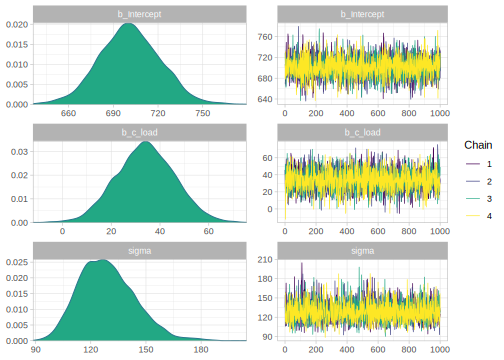
\includegraphics{bookdown_files/figure-latex/posteriorsloadpupilsize-1.pdf}
\caption{\label{fig:posteriorsloadpupilsize}Posterior distributions of the parameters in the brms model \texttt{fit\_pupil}, along with the corresponding trace plots.}
\end{figure}

\begin{Shaded}
\begin{Highlighting}[]
\NormalTok{fit_pupil}
\end{Highlighting}
\end{Shaded}

\begin{verbatim}
## ...
## Population-Level Effects: 
##           Estimate Est.Error l-95% CI u-95% CI Rhat Bulk_ESS Tail_ESS
## Intercept   701.25     20.61   660.51   742.15 1.00     3297     2732
## c_load       33.59     11.80    10.67    57.10 1.00     4247     3307
## 
## Family Specific Parameters: 
##       Estimate Est.Error l-95% CI u-95% CI Rhat Bulk_ESS Tail_ESS
## sigma   128.91     15.12   103.30   162.15 1.00     3187     3247
## 
## ...
\end{verbatim}

In the next section, we discuss how one can communicate the relevant information from the model.

\Begin{extra}

\begin{theorem}
\protect\hypertarget{thm:intercept}{}{\label{thm:intercept} }\textbf{Intercepts in \texttt{brms}}
\end{theorem}

When we set up a prior for the intercept in \texttt{brms}, we actually set a prior for an intercept assuming that all the predictors are centered. This means that when predictors are not centered (and only then), there is a mismatch between the interpretation of the intercept as returned in the output of \texttt{brms} and the interpretation of the intercept with respect to its prior specification. In this case, only the intercept in the output corresponds to the formula in the \texttt{brms} call. However, as we show below, when the intercept is much larger than the effects that we are considering in the formula (what we generally call \(\beta\)), this discrepancy hardly matters.

The reason for this mismatch when our predictors are uncentered is that \texttt{brms} increases sampling efficiency by automatically centering all the predictors internally (that is the population-level design matrix \(X\) is internally centered around its column means when \texttt{brms} fits a model). This did not matter in our previous examples because we centered our predictor (or we had none), but it might matter if we want to have uncentered predictors. In the design we are discussing, a non-centered predictor of load will mean that the intercept, \(\alpha\), has a straightforward interpretation: the \(\alpha\) is the mean pupil size when there is no attention load. This is in contrast with the centered version presented before, where the intercept \(\alpha\) represents the pupil size for the average load of \texttt{2.44} (\texttt{c\_load\ =\ 0}). The difference between the non-centered model (below) and the centered version presented before is depicted in Figure \ref{fig:centered-non-centered}.

Suppose that we are quite sure that the prior values for the no load condition (i.e., condition is non-centered) fall between 400 and 1200 ms. In that case, the following prior could be set for \(\alpha\): \(\mathit{Normal}(800,200)\). In this case, the model becomes:

\begin{Shaded}
\begin{Highlighting}[]
\NormalTok{prior_nc <-}\StringTok{ }\KeywordTok{c}\NormalTok{(}
  \KeywordTok{prior}\NormalTok{(}\KeywordTok{normal}\NormalTok{(}\DecValTok{800}\NormalTok{, }\DecValTok{200}\NormalTok{), }\DataTypeTok{class =}\NormalTok{ b, }\DataTypeTok{coef =}\NormalTok{ Intercept),}
  \KeywordTok{prior}\NormalTok{(}\KeywordTok{normal}\NormalTok{(}\DecValTok{0}\NormalTok{, }\DecValTok{1000}\NormalTok{), }\DataTypeTok{class =}\NormalTok{ sigma),}
  \KeywordTok{prior}\NormalTok{(}\KeywordTok{normal}\NormalTok{(}\DecValTok{0}\NormalTok{, }\DecValTok{100}\NormalTok{), }\DataTypeTok{class =}\NormalTok{ b, }\DataTypeTok{coef =}\NormalTok{ load)}
\NormalTok{)}

\NormalTok{fit_pupil_non_centered <-}\StringTok{ }\KeywordTok{brm}\NormalTok{(p_size }\OperatorTok{~}\StringTok{ }\DecValTok{0} \OperatorTok{+}\StringTok{ }\NormalTok{Intercept }\OperatorTok{+}\StringTok{ }\NormalTok{load,}
  \DataTypeTok{data =}\NormalTok{ df_pupil,}
  \DataTypeTok{family =} \KeywordTok{gaussian}\NormalTok{(),}
  \DataTypeTok{prior =}\NormalTok{ prior_nc}
\NormalTok{)}
\end{Highlighting}
\end{Shaded}



\begin{figure}[H]
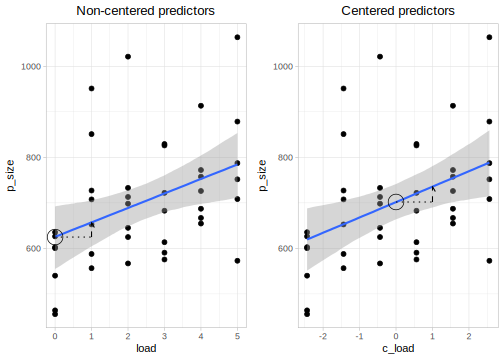
\includegraphics{bookdown_files/figure-latex/centered-non-centered-1} \caption{Regression lines for the non-centered and centered linear regressions. The intercept (or \(\alpha\)) represented by a circle is positioned differently depending on the centering, whereas the slope (or \(\beta\)) represented by a vertical dashed line has the same magnitude in both models.}\label{fig:centered-non-centered}
\end{figure}

When the predictor is non-centered as shown above, the regular centered intercept is removed by adding \texttt{0} to the formula, and by replacing the intercept with the ``actual'' intercept we want to set priors on with \texttt{Intercept}. The word \texttt{Intercept} is a reserved word; we cannot name any predictor with this name. This new parameter is also of the class \texttt{b}, so its prior needs to be defined accordingly. Once we use \texttt{0\ +\ Intercept\ +\ ..}, the intercept is not calculated with predictors that are automatically centered any more.

The output below shows that, as expected, although the posterior for the intercept has changed noticeably, the posterior for the effect of load remains virtually unchanged.

\begin{Shaded}
\begin{Highlighting}[]
\KeywordTok{posterior_summary}\NormalTok{(fit_pupil_non_centered,}
                  \DataTypeTok{variable =} \KeywordTok{c}\NormalTok{(}\StringTok{"b_Intercept"}\NormalTok{, }\StringTok{"b_load"}\NormalTok{))}
\end{Highlighting}
\end{Shaded}

\begin{verbatim}
##             Estimate Est.Error   Q2.5 Q97.5
## b_Intercept    624.3      35.4 555.36 693.1
## b_load          32.3      12.0   9.02  55.8
\end{verbatim}

Notice the following potential pitfall. A model like the one below will fit a non-centered load predictor, but will assign a prior of \(\mathit{Normal}(800,200)\) to the intercept of a model that assumes a centered predictor, \(\alpha_{centered}\), and not the current intercept, \(\alpha\).

\begin{Shaded}
\begin{Highlighting}[]
\NormalTok{fit_pupil_wrong <-}\StringTok{ }\KeywordTok{brm}\NormalTok{(p_size }\OperatorTok{~}\StringTok{ }\DecValTok{1} \OperatorTok{+}\StringTok{ }\NormalTok{load,}
  \DataTypeTok{data =}\NormalTok{ df_pupil,}
  \DataTypeTok{family =} \KeywordTok{gaussian}\NormalTok{(),}
  \DataTypeTok{prior =}\NormalTok{ prior_nc}
\NormalTok{)}
\end{Highlighting}
\end{Shaded}

What does it mean to set a prior to \(\alpha_{centered}\) in a model that doesn't include \(\alpha_{centered}\)?

The fitted (expected) values of the non-centered model and the centered one are identical, that is, the values of the response distribution without the residual error are identical for both models:

\begin{equation}
\alpha + load_n \cdot \beta = \alpha_{centered} + (load_n - mean(load)) \cdot \beta 
\label{eq:fitted}
\end{equation}

The left side of Equation \eqref{eq:fitted} refers to the expected values based on our current non-centered model, and the right side refers to the expected values based on the centered model. We can re-arrange terms to understand what the effect is of a prior on \(\alpha_{centered}\) in our model that doesn't include \(\alpha_{centered}\).

\begin{equation}
\begin{aligned}
\alpha + load_n \cdot \beta &= \alpha_{centered} + load_n\cdot \beta - mean(load) \cdot \beta\\
\alpha  &= \alpha_{centered}  - mean(load) \cdot \beta\\
\alpha + mean(load) \cdot \beta  &= \alpha_{centered}  
\end{aligned}
\end{equation}

That means that in the centered model, we are actually setting our prior to \(\alpha + mean(load) \cdot \beta\).
When \(\beta\) is very small (or the means of our predictors are very small because they might be ``almost'' centered), and the prior for \(\alpha\) is very wide, we might hardly notice the difference between setting a prior to \(\alpha_{centered}\) or to our actual \(\alpha\) in a non-centered model (especially if the likelihood dominates anyway). But it is important to pay attention to what the parameters represent that we are setting priors on.

In our example analyses in this book, we will always center our predictors.

\End{extra}

\hypertarget{how-to-communicate-the-results}{%
\subsection{How to communicate the results?}\label{how-to-communicate-the-results}}

We want to answer our research question ``What is the effect of attentional load on the subject's pupil size?'' For that we'll need to examine what happens with the posterior distribution of \(\beta\), which is printed out as \texttt{c\_load} in the summary of \texttt{brms}. The summary of the posterior tells us that the most likely values of \(\beta\) will be around the mean of the posterior, 33.59, and we can be 95\% certain that the value of \(\beta\), given the model and the data, lies between 10.67 and 57.1.

We see that as the attentional load increases, the pupil size of the subject becomes larger. If we want to determine how likely it is that the pupil size increased rather than decreased, we can examine the proportion of samples above zero. (The intercept and the slopes are always preceded by \texttt{b\_} in \texttt{brms}. One can see all the names of parameters being estimated with \texttt{variables()}.)

\begin{Shaded}
\begin{Highlighting}[]
\KeywordTok{mean}\NormalTok{(}\KeywordTok{as_draws_df}\NormalTok{(fit_pupil)}\OperatorTok{$}\NormalTok{b_c_load }\OperatorTok{>}\StringTok{ }\DecValTok{0}\NormalTok{)}
\end{Highlighting}
\end{Shaded}

\begin{verbatim}
## [1] 0.998
\end{verbatim}

\textbf{This high probability does not mean that the effect of load is non-zero.} It means instead that it's much more likely that the effect is positive rather than negative. In order to claim that the effect is likely to be non-zero, we would have to compare the model with an alternative model in which the model assumes that the effect of load is \(0\). We'll come back to this issue in the model comparison chapter \ref{ch:comparison}.

\hypertarget{sec:pupiladq}{%
\subsection{Descriptive adequacy}\label{sec:pupiladq}}

Our model converged and we obtained a posterior distribution. There is, however, no guarantee that our model is good enough to represent our data. We can use posterior predictive checks to check the descriptive adequacy of the model.

Sometimes it's useful to customize the posterior predictive check to visualize the fit of our model. We iterate over the different loads (e.g, 0 to 4), and we show the prior predictive distributions based on 1000 simulations for each load together with the observed pupil sizes in Figure \ref{fig:postpreddens}. We don't have enough data to derive a strong conclusion: both the predictive distributions and our data look very widely spread out, and it's hard to tell if the distribution of the observations could have been generated by our model. For now we can say that it doesn't look too bad.



\begin{Shaded}
\begin{Highlighting}[]
\ControlFlowTok{for}\NormalTok{ (l }\ControlFlowTok{in} \DecValTok{0}\OperatorTok{:}\DecValTok{4}\NormalTok{) \{}
\NormalTok{  df_sub_pupil <-}\StringTok{ }\KeywordTok{filter}\NormalTok{(df_pupil, load }\OperatorTok{==}\StringTok{ }\NormalTok{l)}
\NormalTok{  p <-}\StringTok{ }\KeywordTok{pp_check}\NormalTok{(fit_pupil,}
    \DataTypeTok{type =} \StringTok{"dens_overlay"}\NormalTok{,}
    \DataTypeTok{ndraws =} \DecValTok{100}\NormalTok{,}
    \DataTypeTok{newdata =}\NormalTok{ df_sub_pupil}
\NormalTok{  ) }\OperatorTok{+}
\StringTok{    }\KeywordTok{geom_point}\NormalTok{(}\DataTypeTok{data =}\NormalTok{ df_sub_pupil, }\KeywordTok{aes}\NormalTok{(}\DataTypeTok{x =}\NormalTok{ p_size, }\DataTypeTok{y =} \FloatTok{0.0001}\NormalTok{)) }\OperatorTok{+}
\StringTok{    }\KeywordTok{ggtitle}\NormalTok{(}\KeywordTok{paste}\NormalTok{(}\StringTok{"load: "}\NormalTok{, l)) }\OperatorTok{+}
\StringTok{    }\KeywordTok{coord_cartesian}\NormalTok{(}\DataTypeTok{xlim =} \KeywordTok{c}\NormalTok{(}\DecValTok{400}\NormalTok{, }\DecValTok{1000}\NormalTok{))}
  \KeywordTok{print}\NormalTok{(p)}
\NormalTok{\}}
\end{Highlighting}
\end{Shaded}

\begin{figure}

{\centering 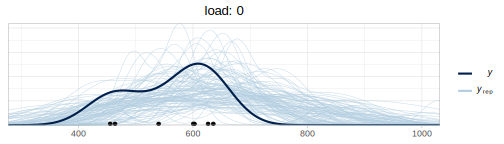
\includegraphics{bookdown_files/figure-latex/postpreddens-1} 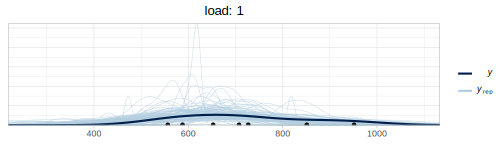
\includegraphics{bookdown_files/figure-latex/postpreddens-2} 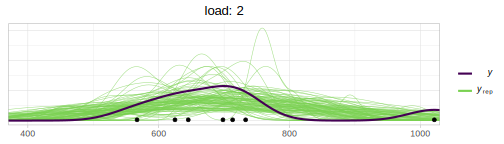
\includegraphics{bookdown_files/figure-latex/postpreddens-3} 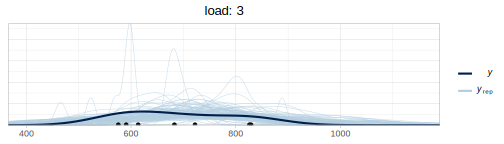
\includegraphics{bookdown_files/figure-latex/postpreddens-4} 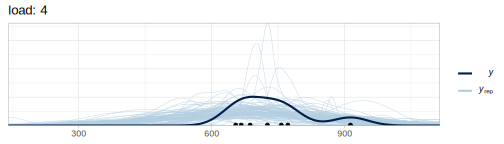
\includegraphics{bookdown_files/figure-latex/postpreddens-5} 

}

\caption{The plot shows 100 predicted distributions with the label \(y_{rep}\), the distribution of pupil size data in black with the label \(y\), and the observed pupil sizes in black dots for the five levels of attentional load.}\label{fig:postpreddens}
\end{figure}

In Figure \ref{fig:postpredmean}, we look instead at the distribution of a summary statistic, such as mean pupil size by load:



\begin{Shaded}
\begin{Highlighting}[]
\ControlFlowTok{for}\NormalTok{ (l }\ControlFlowTok{in} \DecValTok{0}\OperatorTok{:}\DecValTok{4}\NormalTok{) \{}
\NormalTok{  df_sub_pupil <-}\StringTok{ }\KeywordTok{filter}\NormalTok{(df_pupil, load }\OperatorTok{==}\StringTok{ }\NormalTok{l)}
\NormalTok{  p <-}\StringTok{ }\KeywordTok{pp_check}\NormalTok{(fit_pupil,}
    \DataTypeTok{type =} \StringTok{"stat"}\NormalTok{,}
    \DataTypeTok{ndraws =} \DecValTok{1000}\NormalTok{,}
    \DataTypeTok{newdata =}\NormalTok{ df_sub_pupil,}
    \DataTypeTok{stat =} \StringTok{"mean"}
\NormalTok{  ) }\OperatorTok{+}
\StringTok{    }\KeywordTok{geom_point}\NormalTok{(}\DataTypeTok{data =}\NormalTok{ df_sub_pupil, }\KeywordTok{aes}\NormalTok{(}\DataTypeTok{x =}\NormalTok{ p_size, }\DataTypeTok{y =} \FloatTok{0.0001}\NormalTok{)) }\OperatorTok{+}
\StringTok{    }\KeywordTok{ggtitle}\NormalTok{(}\KeywordTok{paste}\NormalTok{(}\StringTok{"load: "}\NormalTok{, l)) }\OperatorTok{+}
\StringTok{    }\KeywordTok{coord_cartesian}\NormalTok{(}\DataTypeTok{xlim =} \KeywordTok{c}\NormalTok{(}\DecValTok{400}\NormalTok{, }\DecValTok{1000}\NormalTok{))}
  \KeywordTok{print}\NormalTok{(p)}
\NormalTok{\}}
\end{Highlighting}
\end{Shaded}

\begin{figure}

{\centering 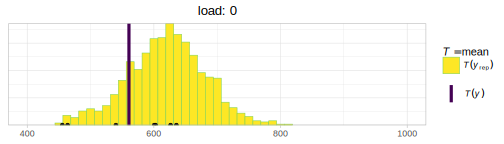
\includegraphics{bookdown_files/figure-latex/postpredmean-1} 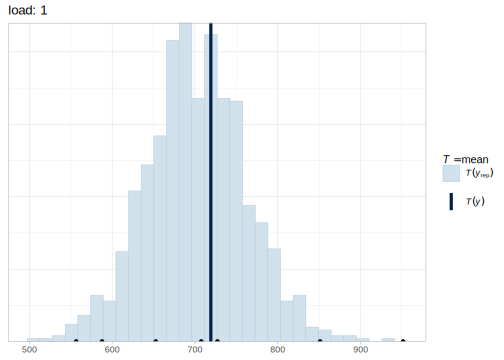
\includegraphics{bookdown_files/figure-latex/postpredmean-2} \includegraphics{bookdown_files/figure-latex/postpredmean-3} \includegraphics{bookdown_files/figure-latex/postpredmean-4} \includegraphics{bookdown_files/figure-latex/postpredmean-5} 

}

\caption{Distribution of posterior predicted means in gray and observed pupil size means in black lines by load.}\label{fig:postpredmean}
\end{figure}

Figure \ref{fig:postpredmean} shows that the observed means for no load and for a load of one are falling in the tails of the distributions. Although our model predicts a monotonic increase of pupil size, the data might be indicating that the relevant difference is simply between no load, and some load. However, given the uncertainty in the posterior predictive distributions and that the observed means are contained somewhere in the predicted distributions, it could be the case that with this model, we are overinterpreting noise.

\hypertarget{sec:trial}{%
\section{Log-normal model: Does trial affect response times?}\label{sec:trial}}

Let us revisit the small experiment from section \ref{sec:simplenormal}, where a subject repeatedly pressed the space bar as fast as possible, without paying attention to the stimuli. We want to know whether the subject tended to speed up (a practice effect) or slow down (a fatigue effect) while pressing the space bar. We'll use the same data set \texttt{df\_spacebar} as before, and we'll center the column \texttt{trial}:

\begin{Shaded}
\begin{Highlighting}[]
\NormalTok{df_spacebar <-}\StringTok{ }\NormalTok{df_spacebar }\OperatorTok
\StringTok{  }\KeywordTok{mutate}\NormalTok{(}\DataTypeTok{c_trial =}\NormalTok{ trial }\OperatorTok{-}\StringTok{ }\KeywordTok{mean}\NormalTok{(trial))}
\end{Highlighting}
\end{Shaded}

\hypertarget{likelihood-and-priors-for-the-log-normal-model}{%
\subsection{Likelihood and priors for the log-normal model}\label{likelihood-and-priors-for-the-log-normal-model}}

If we assume that response times are log-normally distributed, we could fit a likelihood such as the following:

\begin{equation}
rt_n \sim \mathit{LogNormal}(\alpha + c\_trial_n \cdot \beta,\sigma)
\label{eq:rtloglik}
\end{equation}

where \(n =1, \ldots, N\), and \(rt\) is the dependent variable (response times in milliseconds). The variable \(N\) represents the total number of data points.

We use the same priors as in section \ref{sec:lognormal} for \(\alpha\) (which is equivalent to \(\mu\) in the previous model) and for \(\sigma\).

\begin{equation}
\begin{aligned}
\alpha &\sim \mathit{Normal}(6, 1.5) \\
\sigma &\sim \mathit{Normal}_+(0, 1)\\
\end{aligned}
\end{equation}

We still need a prior for \(\beta\). Effects are multiplicative rather than additive when we assume a log-normal likelihood, and that means that we need to take into account \(\alpha\) in order to interpret \(\beta\); for details, see Box \ref{thm:lognormal}. We are going to try to understand how all our priors interact, by generating some prior predictive distributions. We start with the following prior centered in zero, a prior agnostic regarding the direction of the effect, which allows for both a slowdown (\(\beta>0\)) or a speedup (\(\beta<0\)):

\begin{equation}
\beta \sim \mathit{Normal}(0, 1)
\end{equation}

This is our first attempt at a prior predictive distribution:

\begin{Shaded}
\begin{Highlighting}[]
\NormalTok{df_spacebar_ref <-}\StringTok{ }\NormalTok{df_spacebar }\OperatorTok
\StringTok{  }\KeywordTok{mutate}\NormalTok{(}\DataTypeTok{rt =} \KeywordTok{runif}\NormalTok{(}\KeywordTok{n}\NormalTok{(), }\DecValTok{0}\NormalTok{, }\DecValTok{10000}\NormalTok{))}
\NormalTok{fit_prior_press_trial <-}\StringTok{ }\KeywordTok{brm}\NormalTok{(rt }\OperatorTok{~}\StringTok{ }\DecValTok{1} \OperatorTok{+}\StringTok{ }\NormalTok{c_trial,}
  \DataTypeTok{data =}\NormalTok{ df_spacebar_ref,}
  \DataTypeTok{family =} \KeywordTok{lognormal}\NormalTok{(),}
  \DataTypeTok{prior =} \KeywordTok{c}\NormalTok{(}
    \KeywordTok{prior}\NormalTok{(}\KeywordTok{normal}\NormalTok{(}\DecValTok{6}\NormalTok{, }\FloatTok{1.5}\NormalTok{), }\DataTypeTok{class =}\NormalTok{ Intercept),}
    \KeywordTok{prior}\NormalTok{(}\KeywordTok{normal}\NormalTok{(}\DecValTok{0}\NormalTok{, }\DecValTok{1}\NormalTok{), }\DataTypeTok{class =}\NormalTok{ sigma),}
    \KeywordTok{prior}\NormalTok{(}\KeywordTok{normal}\NormalTok{(}\DecValTok{0}\NormalTok{, }\DecValTok{1}\NormalTok{), }\DataTypeTok{class =}\NormalTok{ b, }\DataTypeTok{coef =}\NormalTok{ c_trial)}
\NormalTok{  ),}
  \DataTypeTok{sample_prior =} \StringTok{"only"}\NormalTok{,}
  \DataTypeTok{control =} \KeywordTok{list}\NormalTok{(}\DataTypeTok{adapt_delta =} \FloatTok{.9}\NormalTok{),}
  \DataTypeTok{iter =} \DecValTok{3000}
\NormalTok{)}
\end{Highlighting}
\end{Shaded}

In order to understand the type of data that we are assuming a priori with the prior of the parameter \(\beta\), we'll plot the median difference between the response times at adjacent trials. As the prior of \(\beta\) gets wider we are going to observe larger differences between adjacent trials. The objective of the prior predictive checks is to calibrate the prior of \(\beta\) to obtain a plausible range of differences.
We are going to plot a distribution of medians because they are less affected by the variance in the posterior predicted distribution than the distribution of mean differences; distributions of means will have much more spread. If we want to make the distribution of means more realistic, we would also need to find a more accurate prior for the scale, \(\sigma\). (Recall that the mean of log-normal distributed values depend on both the location, \(\mu\) and the scale, \(\sigma\), of the distribution.) To plot the median effect, we first define a function that calculates the difference between adjacent trials, and then applies the median to the result. We use that function in \texttt{pp\_check} and we show the results in Figure \ref{fig:priorbeta}. As expected, it is centered on zero (as our prior), but we see that the distribution of possible medians for the effect is too widely spread out and includes values that are too extreme.



\begin{Shaded}
\begin{Highlighting}[]
\NormalTok{median_diff <-}\StringTok{ }\ControlFlowTok{function}\NormalTok{(x) \{}
  \KeywordTok{median}\NormalTok{(x }\OperatorTok{-}\StringTok{ }\KeywordTok{lag}\NormalTok{(x), }\DataTypeTok{na.rm =} \OtherTok{TRUE}\NormalTok{)}
\NormalTok{\}}
\KeywordTok{pp_check}\NormalTok{(fit_prior_press_trial,}
         \DataTypeTok{type =} \StringTok{"stat"}\NormalTok{,}
         \DataTypeTok{stat =} \StringTok{"median_diff"}\NormalTok{,}
  \CommentTok{# each bin has a width of 500ms       }
         \DataTypeTok{binwidth =} \DecValTok{500}\NormalTok{) }\OperatorTok{+}
\StringTok{  }\CommentTok{# cut the top of the plot to improve its scale}
\StringTok{  }\KeywordTok{coord_cartesian}\NormalTok{(}\DataTypeTok{ylim =} \KeywordTok{c}\NormalTok{(}\DecValTok{0}\NormalTok{, }\DecValTok{50}\NormalTok{))}
\end{Highlighting}
\end{Shaded}

\begin{figure}
\centering
\includegraphics{bookdown_files/figure-latex/priorbeta-1.pdf}
\caption{\label{fig:priorbeta}Prior predictive distribution of the median effect of the model defined in \ref{sec:trial} with \(\beta \sim \mathit{Normal}(0, 1)\).}
\end{figure}

We repeat the same procedure with \(\beta \sim \mathit{Normal}(0,0.01)\), and we plot it in Figure \ref{fig:priorbeta2}. The prior predictive distribution shows us that the prior is still quite vague, it is, however at least in the right order of magnitude.



\begin{figure}
\centering
\includegraphics{bookdown_files/figure-latex/priorbeta2-1.pdf}
\caption{\label{fig:priorbeta2}Prior predictive distribution of the median difference in response times between adjacent trials based on the model defined in \ref{sec:trial} with \(\beta \sim \mathit{Normal}(0, 0.01)\).}
\end{figure}

Prior selection might look daunting and a lot of work. However, this work is usually done only the first time we encounter an experimental paradigm; besides, priors can be informed by the estimates from previous experiments (even maximum likelihood estimates from frequentist models can be useful). We will generally use very similar (or identical priors) for analyses dealing with the same type of task. When in doubt, a sensitivity analysis (see section \ref{sec:sensitivity}) can tell us whether the posterior distribution depends unintentionally strongly on our prior selection. We will return to the issue of prior selection in chapter \ref{ch:priors}.

\Begin{extra}

\begin{theorem}
\protect\hypertarget{thm:lognormal}{}{\label{thm:lognormal} }\textbf{Understanding the Log-normal likelihood}
\end{theorem}

It is important to understand what we are assuming with our log-normal likelihood. Formally, if a random variable \(Z\) is normally distributed with mean \(\mu\) and variance \(\sigma^2\), then the transformed random variable \(Y = \exp(Z)\) is log-normally distributed and has density:

\begin{equation}
\mathit{LogNormal}(y|\mu,\sigma)=f(z)= \frac{1}{\sqrt{2\pi \sigma^2}y} \exp \left(-\frac{(\log(y)-\mu)^2}{2\sigma^2} \right)
\end{equation}

As explained in section \ref{sec:lnfirst}, the model from Equation \eqref{eq:rtloglik} is equivalent to the following:

\begin{equation}
\log(rt_n) \sim \mathit{Normal}(\alpha + c\_trial_n \cdot \beta,\sigma)\\
\label{eq:aX}
\end{equation}

The family of normal distributions is closed under linear transformations: that is, if \(X\) is normally distributed with mean \(\mu\) and standard deviation \(\sigma\), then (for any real numbers \(a\) and \(b\)), \(a X + b\) is also normally distributed, with mean \(a \mu +b\) (and standard deviation \(\sqrt{a^2\sigma^2}=|a|\sigma\)).

This means that, assuming \(Z \sim \mathit{Normal}(\alpha, \sigma)\), Equation \eqref{eq:aX} can be re-written as follows:

\begin{equation}
\log(rt_n) = Z + c\_trial_n \cdot \beta
\label{eq:rtlogliknoncen}
\end{equation}

We exponentiate both sides, and we use the property of exponents that \(\exp(x+y)\) is equal to \(\exp(x) \cdot \exp(y)\), and we set \(Y =\exp(Z)\).

\begin{equation}
\begin{aligned}
rt_n &= \exp \big(Z  + c\_trial_n \cdot \beta\big) \\
rt_n &= \exp(Z )   \cdot \exp\big(c\_trial_n \cdot \beta\big) \\
rt_n &= Y \cdot \exp\big(c\_trial_n \cdot \beta\big) 
\end{aligned}
\end{equation}

The last equation has two terms being multiplied, the first one, \(Y\), is telling us that we are assuming that response times are log-normally distributed with a median of \(\exp(\alpha)\), the second term, \(\exp(c\_trial_n \cdot \beta)\) is telling us that the effect of trial number is multiplicative and grows or decays exponentially with the trial number. This has two important consequences:

\begin{enumerate}
\def\labelenumi{\arabic{enumi}.}
\item
  Different values of the intercept, \(\alpha\), given the same \(\beta\), will affect the difference in response times for two adjacent trials (this is in contrast to what happens with an additive model such as normal likelihood); see Figure \ref{fig:logexp}. This is because, unlike in the additive case, the intercept doesn't cancel out:

  \begin{itemize}
  \item
    Additive case:

    \begin{equation}
    \begin{aligned}
    & (\alpha + trial_n \cdot \beta) - (\alpha + trial_{n-1} \cdot \beta) = \\
    &=\alpha -\alpha + ( trial_n - trial_{n-1} ) \cdot \beta\\
    &= ( trial_n - trial_{n-1} ) \cdot \beta
    \end{aligned}
    \end{equation}
  \item
    Multiplicative case:

    \begin{equation}
    \begin{aligned}
       &\exp(\alpha) \cdot \exp(trial_n \cdot \beta) -\exp(\alpha) \cdot \exp(trial_{n-1} \cdot \beta) =\\ 
       &= \exp(\alpha) \big(\exp(trial_n  \cdot \beta)  - \exp(trial_{n-1}\cdot \beta) \big)\\
       &\neq \big(\exp(trial_n)  - \exp(trial_{n-1})  \big) \cdot \exp(\beta) 
    \end{aligned}
       \end{equation}
  \end{itemize}
\end{enumerate}



\begin{figure}[H]
  \includegraphics{bookdown_files/figure-latex/logexp-1} \caption{Fitted value of the difference in reaction time between two adjacent trials, when \(\beta=0.01\) and \(\alpha\) lies between 0.1 and 15. The graph shows how changes in the intercept lead to changes in the difference in response times between trials, even if \(\beta\) is fixed.}\label{fig:logexp}
  \end{figure}

\begin{enumerate}
\def\labelenumi{\arabic{enumi}.}
\setcounter{enumi}{1}
\tightlist
\item
  As the trial number increases, the same value of \(\beta\) will have a very different impact on the original scale of the dependent variable: Any (fixed) negative value for \(\beta\) will lead to exponential decay and any (fixed) positive value will lead to exponential growth; see Figure \ref{fig:expgd}.
\end{enumerate}



\begin{figure}[H]
\includegraphics{bookdown_files/figure-latex/expgd-1} \caption{Fitted value of the dependent variable (response times in ms) as function of trial number, when (A) \(\beta = -0.01\), exponential decay, and when (B) \(\beta =0.01\), exponential growth.}\label{fig:expgd}
\end{figure}

Can exponential growth or decay make sense? We need to consider that if they do make sense, they will be an approximation valid for a specific range of values, at some point we will expect a ceiling or a floor effect: response times cannot truly be 0 milliseconds, or take several minutes. However, in our specific model, exponential growth or decay \emph{by trial} is probably a bad approximation: We will predict that our subject will take extremely long (if \(\beta >0\)) or extremely short (if \(\beta <0\)) time in pressing the space bar in a relatively low number of trials. This doesn't mean that the likelihood is wrong by itself, but it does mean that at least we need to put a cap on the growth or decay of our experimental manipulation. We can do this if the exponential growth or decay is a function of, for example, log-transformed trial numbers:

\begin{equation}
rt_n \sim \mathit{LogNormal}(\alpha + c\_\log\_trial_n \cdot \beta,\sigma)\\
\end{equation}



\begin{figure}[H]
\includegraphics{bookdown_files/figure-latex/expgd2-1} \caption{Fitted value of the dependent variable (response times in ms) as function of the natural logarithm of the trial number, when (A) \(\beta=-0.01\), exponential decay, and when (B) \(\beta =.01\), exponential growth.}\label{fig:expgd2}
\end{figure}

\textbf{Log-normal distributions everywhere}

The normal distribution is most often assumed to describe the random variation that occurs in the data from many scientific disciplines. However, most measurements actually show skewed distributions. Limpert, Stahel, and Abbt (\protect\hyperlink{ref-limpertLognormalDistributionsSciences2001}{2001}) discuss the log-normal distribution in scientific disciplines and how diverse type of data, from lengths of latent periods of infectious diseases to distribution of mineral resources in the Earth's crust, including even body height--the quintessential example of a normal distribution--closely fit the log-normal distribution.

Limpert, Stahel, and Abbt (\protect\hyperlink{ref-limpertLognormalDistributionsSciences2001}{2001}) point out that because a random variable that results from multiplying many independent variables has an approximate log-normal distribution, the most basic indicator of the importance of the log-normal distribution may be very general: Chemistry and physics are fundamental in life, and the prevailing operation in the laws of these disciplines is multiplication rather than addition.

Furthermore, at many physiological and anatomical levels in the brain, the distribution of numerous parameters is in fact strongly skewed with a heavy tail, suggesting that skewed (typically log-normal) distributions are fundamental to structural and functional brain organization. This might be explained given that the majority of interactions in highly interconnected systems, especially in biological systems, are multiplicative and synergistic rather than additive (Buzsáki and Mizuseki \protect\hyperlink{ref-buzsakiLogdynamicBrainHow2014}{2014}).

Does the log-normal distribution make sense for response times?
It has been long noticed that the log-normal distribution often provides a good fit to response times
distributions (Brée \protect\hyperlink{ref-breeDistributionProblemsolvingTimes1975}{1975}; Ulrich and Miller \protect\hyperlink{ref-ulrichEffectsTruncationReaction1994}{1994}).
One advantage of assuming log-normally distributed response times (but, in fact, this is true for many skewed distributions) is that it entails that the standard deviation of the reaction time distribution will increase with the mean, as has been observed in empirical distributions of response times (Wagenmakers, Grasman, and Molenaar \protect\hyperlink{ref-wagenmakersRelationMeanVariance2005}{2005}). Interestingly, it turns out that log-normal response times are also easily generated by certain process models. Ulrich and Miller (\protect\hyperlink{ref-ulrichInformationProcessingModels1993}{1993}) show, for example, that models in which response times are determined by a series of processes cascading activation from an input level to an output level (usually passing through a number of intervening processing levels along the way) can generate log-normally distributed response times.

\End{extra}

\hypertarget{the-brms-model-1}{%
\subsection{\texorpdfstring{The \texttt{brms} model}{The brms model}}\label{the-brms-model-1}}

We are now relatively satisfied with the priors for our model, and we can fit the model of the effect of trial as a button-pressing using \texttt{brms}. We need to specify that the family is \texttt{lognormal()}.

\begin{Shaded}
\begin{Highlighting}[]
\NormalTok{fit_press_trial <-}\StringTok{ }\KeywordTok{brm}\NormalTok{(rt }\OperatorTok{~}\StringTok{ }\DecValTok{1} \OperatorTok{+}\StringTok{ }\NormalTok{c_trial,}
  \DataTypeTok{data =}\NormalTok{ df_spacebar,}
  \DataTypeTok{family =} \KeywordTok{lognormal}\NormalTok{(),}
  \DataTypeTok{prior =} \KeywordTok{c}\NormalTok{(}
    \KeywordTok{prior}\NormalTok{(}\KeywordTok{normal}\NormalTok{(}\DecValTok{6}\NormalTok{, }\FloatTok{1.5}\NormalTok{), }\DataTypeTok{class =}\NormalTok{ Intercept),}
    \KeywordTok{prior}\NormalTok{(}\KeywordTok{normal}\NormalTok{(}\DecValTok{0}\NormalTok{, }\DecValTok{1}\NormalTok{), }\DataTypeTok{class =}\NormalTok{ sigma),}
    \KeywordTok{prior}\NormalTok{(}\KeywordTok{normal}\NormalTok{(}\DecValTok{0}\NormalTok{, }\FloatTok{.01}\NormalTok{), }\DataTypeTok{class =}\NormalTok{ b, }\DataTypeTok{coef =}\NormalTok{ c_trial)}
\NormalTok{  )}
\NormalTok{)}
\end{Highlighting}
\end{Shaded}

Instead of printing out the complete output from the model, look at the estimates from the posteriors for the parameters \(\alpha\), \(\beta\), and \(\sigma\). These parameters are on the log scale:

\begin{Shaded}
\begin{Highlighting}[]
\KeywordTok{posterior_summary}\NormalTok{(fit_press_trial)[, }\KeywordTok{c}\NormalTok{(}\StringTok{"Estimate"}\NormalTok{, }\StringTok{"Q2.5"}\NormalTok{, }\StringTok{"Q97.5"}\NormalTok{)]}
\end{Highlighting}
\end{Shaded}

\begin{verbatim}
##                 Estimate         Q2.5        Q97.5
## b_Intercept     5.117908     5.104991     5.130196
## b_c_trial       0.000522     0.000404     0.000641
## sigma           0.123096     0.113965     0.132418
## lp__        -1603.668497 -1606.855607 -1602.288734
\end{verbatim}

The posterior distributions can be plotted to obtain a graphical summary of all the parameters in the model (Figure \ref{fig:posteriorsfitpresstrial}:

\begin{Shaded}
\begin{Highlighting}[]
\KeywordTok{plot}\NormalTok{(fit_press_trial)}
\end{Highlighting}
\end{Shaded}

\begin{figure}
\centering
\includegraphics{bookdown_files/figure-latex/posteriorsfitpresstrial-1.pdf}
\caption{\label{fig:posteriorsfitpresstrial}Posterior distributions of the model of the effect of trial on button-pressing.}
\end{figure}

Next, we turn to the question of what we can report as our results, and what we can conclude from the data.

\hypertarget{how-to-communicate-the-results-1}{%
\subsection{How to communicate the results?}\label{how-to-communicate-the-results-1}}

As shown above, the first step is to summarize the posteriors in a table or graphically (or both). If the research relates to the effect estimated by the model, the posterior of \(\beta\) can be summarized in the following way: \(\hat\beta = 0.00052\), 95\% CrI = \([ 0.0004 , 0.00064 ]\).

The effect is easier to interpret in milliseconds. We can transform the estimates back to the millisecond scale from the log scale, but we need to take into account that the scale is not linear, and that the effect between two button presses will differ depending on where we are in the experiment.

We will have a certain estimate if we consider the difference between response times in a trial at the middle of the experiment (when the centered trial number is zero) and the previous one (when the centered trial number is minus one).

\begin{Shaded}
\begin{Highlighting}[]
\NormalTok{alpha_samples <-}\StringTok{ }\KeywordTok{as_draws_df}\NormalTok{(fit_press_trial)}\OperatorTok{$}\NormalTok{b_Intercept}
\NormalTok{beta_samples <-}\StringTok{ }\KeywordTok{as_draws_df}\NormalTok{(fit_press_trial)}\OperatorTok{$}\NormalTok{b_c_trial}
\NormalTok{effect_middle_ms <-}\StringTok{ }\KeywordTok{exp}\NormalTok{(alpha_samples) }\OperatorTok{-}
\StringTok{  }\KeywordTok{exp}\NormalTok{(alpha_samples }\OperatorTok{-}\StringTok{ }\DecValTok{1} \OperatorTok{*}\StringTok{ }\NormalTok{beta_samples)}
\CommentTok{## ms effect in the middle of the expt}
\CommentTok{## (mean trial vs. mean trial - 1)}
\KeywordTok{c}\NormalTok{(}
  \DataTypeTok{mean =} \KeywordTok{mean}\NormalTok{(effect_middle_ms),}
  \KeywordTok{quantile}\NormalTok{(effect_middle_ms, }\KeywordTok{c}\NormalTok{(}\FloatTok{0.025}\NormalTok{, }\FloatTok{0.975}\NormalTok{))}
\NormalTok{)}
\end{Highlighting}
\end{Shaded}

\begin{verbatim}
##   mean   2.5%  97.5% 
## 0.0872 0.0675 0.1068
\end{verbatim}

We will obtain different estimate if we consider the difference between the second and the first trial:

\begin{Shaded}
\begin{Highlighting}[]
\NormalTok{first_trial <-}\StringTok{ }\KeywordTok{min}\NormalTok{(df_spacebar}\OperatorTok{$}\NormalTok{c_trial)}
\NormalTok{second_trial <-}\StringTok{ }\KeywordTok{min}\NormalTok{(df_spacebar}\OperatorTok{$}\NormalTok{c_trial) }\OperatorTok{+}\StringTok{ }\DecValTok{1}
\NormalTok{effect_beginning_ms <-}
\StringTok{  }\KeywordTok{exp}\NormalTok{(alpha_samples }\OperatorTok{+}\StringTok{ }\NormalTok{second_trial }\OperatorTok{*}\StringTok{ }\NormalTok{beta_samples) }\OperatorTok{-}
\StringTok{  }\KeywordTok{exp}\NormalTok{(alpha_samples }\OperatorTok{+}\StringTok{ }\NormalTok{first_trial }\OperatorTok{*}\StringTok{ }\NormalTok{beta_samples)}
\CommentTok{## ms effect from first to second trial:}
\KeywordTok{c}\NormalTok{(}
  \DataTypeTok{mean =} \KeywordTok{mean}\NormalTok{(effect_beginning_ms),}
  \KeywordTok{quantile}\NormalTok{(effect_beginning_ms, }\KeywordTok{c}\NormalTok{(}\FloatTok{0.025}\NormalTok{, }\FloatTok{0.975}\NormalTok{))}
\NormalTok{)}
\end{Highlighting}
\end{Shaded}

\begin{verbatim}
##   mean   2.5%  97.5% 
## 0.0793 0.0628 0.0952
\end{verbatim}

So far we converted the estimates to obtain median effects, that's why we used \(exp(\cdot)\), if we want to obtain mean effects we need to take into account \(\sigma\), since we need to calculate \(exp(\cdot + \sigma^2/2)\). However, we can also use the built-in function \texttt{fitted()}. We can consider again the difference between the second and the first trial this time using \texttt{fitted()}.

First, define for which observations we want to obtain the fitted values in millisecond scale. If we are interested in the difference between the second and first trial, create a data frame with their centered versions.

\begin{Shaded}
\begin{Highlighting}[]
\NormalTok{newdata_}\DecValTok{1}\NormalTok{ <-}\StringTok{ }\KeywordTok{data.frame}\NormalTok{(}\DataTypeTok{c_trial =} \KeywordTok{c}\NormalTok{(first_trial, second_trial))}
\end{Highlighting}
\end{Shaded}

Second, use \texttt{fitted()} on the brms object, including the new data, and setting the \texttt{summary} parameter to \texttt{FALSE}. The first column contains the posterior samples transformed into milliseconds of the first trial, and the second column of the second trial.

\begin{Shaded}
\begin{Highlighting}[]
\NormalTok{beginning <-}\StringTok{ }\KeywordTok{fitted}\NormalTok{(fit_press_trial,}
                 \DataTypeTok{newdata =}\NormalTok{ newdata_}\DecValTok{1}\NormalTok{,}
                 \DataTypeTok{summary =} \OtherTok{FALSE}\NormalTok{)}
\KeywordTok{head}\NormalTok{(beginning, }\DecValTok{3}\NormalTok{)}
\end{Highlighting}
\end{Shaded}

\begin{verbatim}
##      [,1] [,2]
## [1,]  154  154
## [2,]  150  150
## [3,]  154  154
\end{verbatim}

Last, calculate the difference between trials, and report mean and 95\% quantiles.

\begin{Shaded}
\begin{Highlighting}[]
\NormalTok{effect_beginning_ms <-}\StringTok{ }\NormalTok{beginning[, }\DecValTok{2}\NormalTok{] }\OperatorTok{-}\StringTok{ }\NormalTok{beginning[,}\DecValTok{1}\NormalTok{]}
\KeywordTok{c}\NormalTok{(}
  \DataTypeTok{mean =} \KeywordTok{mean}\NormalTok{(effect_beginning_ms),}
  \KeywordTok{quantile}\NormalTok{(effect_beginning_ms, }\KeywordTok{c}\NormalTok{(}\FloatTok{0.025}\NormalTok{, }\FloatTok{0.975}\NormalTok{))}
\NormalTok{)}
\end{Highlighting}
\end{Shaded}

\begin{verbatim}
##   mean   2.5%  97.5% 
## 0.0799 0.0632 0.0960
\end{verbatim}

Given that \(\sigma\) is much smaller than \(\mu\), \(\sigma\) doesn't have a large influence on the mean effects, and the mean and 95\% CrI of the mean and median effects are quite similar.

We see that no matter how we calculate the trial effect, there is a slowdown. When reporting the results of these analyses, one should present the posterior mean and the 95\% credible interval and then reason about whether the observed estimates are consistent with the prediction from the theory being investigated.

The practical relevance of the effect for the research question can be important too. For example, only after 100 button presses do we see a slowdown of 9 ms on average (\(0.087 \cdot 100\)), with a 95\% credible interval ranging from 6.746 to 10.679. We need to consider whether our uncertainty of this estimate, and the estimated mean effect have any scientific relevance. Such relevance can be established by considering the previous literature, predictions from a quantitative model, or other expert domain knowledge. Sometimes, a quantitative meta-analysis is helpful; for examples, see Jäger, Engelmann, and Vasishth (\protect\hyperlink{ref-JaegerEngelmannVasishth2017}{2017}), Mahowald et al. (\protect\hyperlink{ref-mahowald2016meta}{2016}), Nicenboim, Roettger, and Vasishth (\protect\hyperlink{ref-NicenboimRoettgeretal}{2018}), and Vasishth et al. (\protect\hyperlink{ref-VasishthetalPLoSOne2013}{2013}). We will discuss meta-analysis in later in the book, in chapter \ref{ch:remame}.

Sometimes, researchers are only interested in establishing that an effect is present or absent; the magnitude and uncertainty of the estimate is of secondary interest. Here, the goal is to argue that there is \textbf{evidence} of a slowdown. The word evidence has a special meaning in statistics (Royall \protect\hyperlink{ref-Royall}{1997}), and in null hypothesis significance testing, a likelihood ratio test is the standard way to argue that one has evidence for an effect. In the Bayesian data analysis context, in order to answer such a question, a Bayes factor analysis must be carried out. We'll come back to this issue in the model comparison chapters \ref{ch:comparison}-\ref{ch:cv}.

\hypertarget{descriptive-adequacy}{%
\subsection{Descriptive adequacy}\label{descriptive-adequacy}}

We look now at the predictions of the model. Since we now know that trial effects are very small, we'll examine predictions of the model for differences in response times between 100 button presses. Similarly as we did for prior predictive checks, we define a function, this time \texttt{median\_diff100()}, that calculates the median difference between a trial \(n\) and a trial \(n+100\). This time we'll compare the observed median difference against the range of predicted differences based on the model and the data rather than only the model as we did for the prior predictions. Below we use virtually the same code that we use for plotting prior predictive checks, but since we now use the fitted model, we'll obtain posterior predictive checks; this is displayed in Figure \ref{fig:posteriorcbeta}.



\begin{Shaded}
\begin{Highlighting}[]
\NormalTok{median_diff100 <-}\StringTok{ }\ControlFlowTok{function}\NormalTok{(x) }\KeywordTok{median}\NormalTok{(x }\OperatorTok{-}\StringTok{ }\KeywordTok{lag}\NormalTok{(x, }\DecValTok{100}\NormalTok{), }\DataTypeTok{na.rm =} \OtherTok{TRUE}\NormalTok{)}
\KeywordTok{pp_check}\NormalTok{(fit_press_trial,}
         \DataTypeTok{type =} \StringTok{"stat"}\NormalTok{,}
         \DataTypeTok{stat =} \StringTok{"median_diff100"}\NormalTok{)}
\end{Highlighting}
\end{Shaded}

\begin{figure}
\centering
\includegraphics{bookdown_files/figure-latex/posteriorcbeta-1.pdf}
\caption{\label{fig:posteriorcbeta}Posterior predictive distribution of the median difference in response times between a trial \(n\) and a trial \(n+100\) based on the model \texttt{fit\_press\_trial} and the observed data.}
\end{figure}

We can conclude that model predictions for differences in response trials between trials are reasonable.

\hypertarget{sec:logistic}{%
\section{Logistic regression: Does set size affect free recall?}\label{sec:logistic}}

In this section, we will learn how the principles we have learned so far can naturally extend to \emph{generalized} linear models (GLMs). We focus on one special case of GLMs that has wide application in linguistics and psychology, logistic regression.

As an example data set, we look at a study investigating the capacity level of working memory. The data are a subset of a data set created by Oberauer (\protect\hyperlink{ref-oberauerWorkingMemoryCapacity2019}{2019}). Each subject was presented word lists of varying lengths (2, 4, 6, and 8 elements), and then was asked to recall a word given its position on the list; see Figure \ref{fig:oberauer}. We will focus on the data from one subject.



\begin{figure}
\includegraphics[width=1\linewidth]{cc_figure/fig1_oberauer_2019_modified} \caption{Flow of events in a trial with memory set size 4 and free recall. Adapted from Oberauer (\protect\hyperlink{ref-oberauerWorkingMemoryCapacity2019}{2019}); licensed under CC BY 4.0.}\label{fig:oberauer}
\end{figure}

It is well-established that as the number of items to be held in working memory increases, performance, that is accuracy, decreases (see Oberauer and Kliegl \protect\hyperlink{ref-oberauerkliegel2001}{2001}, among others). We will investigate whether we can investigate this finding with data from only one subject.

The data can be found in \texttt{df\_recall} in the package \texttt{bcogsci}. The code below loads the data, centers the predictor \texttt{set\_size}, and briefly explores the data set.

\begin{Shaded}
\begin{Highlighting}[]
\KeywordTok{data}\NormalTok{(}\StringTok{"df_recall"}\NormalTok{)}
\NormalTok{df_recall <-}\StringTok{ }\NormalTok{df_recall }\OperatorTok
\StringTok{  }\KeywordTok{mutate}\NormalTok{(}\DataTypeTok{c_set_size =}\NormalTok{ set_size }\OperatorTok{-}\StringTok{ }\KeywordTok{mean}\NormalTok{(set_size))}
\CommentTok{# Set sizes in the data set:}
\NormalTok{df_recall}\OperatorTok{$}\NormalTok{set_size }\OperatorTok
\StringTok{  }\KeywordTok{unique}\NormalTok{() }\OperatorTok\StringTok{ }\KeywordTok{sort}\NormalTok{()}
\end{Highlighting}
\end{Shaded}

\begin{verbatim}
## [1] 2 4 6 8
\end{verbatim}

\begin{Shaded}
\begin{Highlighting}[]
\CommentTok{# Trials by set size}
\NormalTok{df_recall }\OperatorTok
\StringTok{  }\KeywordTok{group_by}\NormalTok{(set_size) }\OperatorTok
\StringTok{  }\KeywordTok{count}\NormalTok{()}
\end{Highlighting}
\end{Shaded}

\begin{verbatim}
## # A tibble: 4 x 2
## # Groups:   set_size [4]
##   set_size     n
##      <int> <int>
## 1        2    23
## 2        4    23
## 3        6    23
## # ... with 1 more row
\end{verbatim}

Here, the column \texttt{correct} records the incorrect vs.~correct responses with \texttt{0} vs \texttt{1}, and the column \texttt{c\_set\_size} records the centered memory set size; these latter scores have continuous values -3, -1, 1, and 3. These continuous values are centered versions of 2, 4, 6, and 8.

\begin{Shaded}
\begin{Highlighting}[]
\NormalTok{df_recall}
\end{Highlighting}
\end{Shaded}

\begin{verbatim}
## # A tibble: 92 x 8
##   subj  set_size correct trial session block tested c_set_size
##   <chr>    <int>   <int> <int>   <int> <int>  <int>      <dbl>
## 1 10           4       1     1       1     1      2         -1
## 2 10           8       0     4       1     1      8          3
## 3 10           2       1     9       1     1      2         -3
## # ... with 89 more rows
\end{verbatim}

We want to model the trial-by-trial accuracy and examine whether the probability of recalling a word is related to the number of words in the set that the subject needs to remember.

\hypertarget{the-likelihood-for-the-logistic-regression-model}{%
\subsection{The likelihood for the logistic regression model}\label{the-likelihood-for-the-logistic-regression-model}}

Recall that the Bernoulli likelihood generates a \(0\) or \(1\) response with a particular probability \(\theta\). For example, one can generate simulated data for \(10\) trials, with a 50\% probability of getting a \(1\) using \texttt{rbern} from the package \texttt{extraDistr}.

\begin{Shaded}
\begin{Highlighting}[]
\KeywordTok{rbern}\NormalTok{(}\DecValTok{10}\NormalTok{, }\DataTypeTok{prob =} \FloatTok{0.5}\NormalTok{)}
\end{Highlighting}
\end{Shaded}

\begin{verbatim}
##  [1] 1 0 1 1 0 1 0 1 1 1
\end{verbatim}

We can therefore define each dependent value \texttt{correct\_n} in the data as being generated from a Bernoulli random variable with probability of success \(\theta_n\).
Here, \(n =1, \ldots, N\) indexes the trial, correct\_n is the dependent variable (0 indicates an incorrect recall and 1 a correct recall), and \(\theta_n\) is the probability of correctly recalling a probe in a given trial \(n\).

\begin{equation}
correct_n \sim \mathit{Bernoulli}(\theta_n)
\label{eq:bernoullilik}
\end{equation}

Since \(\theta_n\) is bounded to be between \(0\) and \(1\) (it is a probability), we cannot just fit a regression model using the normal (or log-normal) likelihood as we did in the preceding examples. Such a model would be inappropriate because it would assume that the data range from \(-\infty\) to \(+\infty\) (or from \(0\) to \(+\infty\)), rather than being limited to zeros and ones.

The generalized linear modeling framework solves this problem by defining a \emph{link function} \(g(\cdot)\) that connects the linear model to the quantity to be estimated (here, the probabilities \(\theta_n\)). The link function used for \(0\), \(1\) responses is called the \emph{logit link}, and is defined as follows.

\begin{equation}
\eta_n = g(\theta_n) = \log\left(\frac{\theta_n}{1-\theta_n}\right)
\end{equation}

The term \(\frac{\theta_n}{1-\theta_n}\) is called the \emph{odds}.\footnote{Odds are defined to be the ratio of the probability of success to the probability of failure. For example, the odds of obtaining a one in a fair six-sided die are \(\frac{1/6}{1-1/6}=1/5\). The odds of obtaining a heads in a fair coin are 1/1.} The logit link function is therefore a log-odds; it maps probability values ranging from \([0,1]\) to real numbers ranging from \(-\infty\) to \(+\infty\). Figure \ref{fig:logisticfun} shows the logit link function, \(\eta = g(\theta)\), and the inverse logit, \(\theta = g^{-1}(\eta)\), which is called the \emph{logistic function}; the relevance of this logistic function will become clear in a moment.

\begin{figure}
\centering
\includegraphics{bookdown_files/figure-latex/logisticfun-1.pdf}
\caption{\label{fig:logisticfun}The logit and inverse logit (logistic) function.}
\end{figure}

The linear model is now fit not to the 0,1 responses as the dependent variable, but to \(\eta_n\), i.e., log-odds, as the dependent variable:

\begin{equation}
\eta_n = \log\left(\frac{\theta_n}{1-\theta_n}\right) = \alpha + \beta \cdot c\_set\_size
\end{equation}

Unlike the linear models, the model is defined so that there is no residual error term (\(\varepsilon\)) in this model. Once \(\eta_n\) is estimated, one can solve the above equation for \(\theta_n\) (in other words, we compute the inverse of the logit function and obtain the estimates on the probability scale). This gives the above-mentioned logistic regression function:

\begin{equation}
\theta_n = g^{-1}(\eta_n) =  \frac{\exp(\eta_n)}{1+\exp(\eta_n)} = \frac{1}{1+exp(-\eta_n)}
\end{equation}

The last equality in the equation above arises by dividing both the numerator and denominator by \(\exp(\eta_n)\).

In summary, the generalized linear model with the logit link fits the following Bernoulli likelihood:

\begin{equation}
correct_n \sim \mathit{Bernoulli}(\theta_n)
\label{eq:bernoullilogislik}
\end{equation}

The model is fit on the log-odds scale, \(\eta_n = \alpha + c\_set\_size_n \cdot \beta\).
Once \(\eta_n\) has been estimated, the inverse logit or the logistic function is used to compute the probability estimates
\(\theta_n = \frac{\exp(\eta_n)}{1+\exp(\eta_n)}\). An example of this calculations will be shown in the next section.

\hypertarget{sec:priorslogisticregression}{%
\subsection{Priors for the logistic regression}\label{sec:priorslogisticregression}}

In order to decide on priors for \(\alpha\) and \(\beta\), we need to take into account that these parameters do not represent probabilities or proportions, but \emph{log-odds}, the x-axis in Figure \ref{fig:logisticfun} (right-hand side figure). As shown in the figure, the relationship between log-odds and probabilities is not linear.

There are two functions in R that implement the logit and inverse logit functions: \texttt{qlogis(p)} for the logit function and \texttt{plogis(x)} for the inverse logit or logistic function.

Now we need to set priors for \(\alpha\) and \(\beta\).
Given that we centered our predictor, the intercept, \(\alpha\), represents the log-odds of correctly recalling one word in a random position for the average set size of five (since \(5 = \frac{2+4+6+8}{4}\)), which, incidentally, was not presented in the experiment. This is one case where the intercept doesn't have a clear interpretation if we leave the prediction uncentered: With non-centered set size, the intercept will be the log-odds of recalling one word in a set of \emph{zero} words.

The prior for \(\alpha\) will depend on how difficult the recall task is. If we are not sure, we could assume that the probability of recalling a word for an average set size, \(\alpha\), is centered in .5 (a 50/50 chance) with a great deal of uncertainty. The \texttt{R} command \texttt{qlogis(.5)} tells us that .5 corresponds to zero in log-odds space. How do we include a great deal of uncertainty? We could look at Figure \ref{fig:logisticfun}, and decide on a standard deviation of 4 in a normal distribution centered in zero:

\begin{equation}
\alpha \sim \mathit{Normal}(0, 4) 
\end{equation}

Let's plot this prior in log-odds and in probability scale by drawing random samples.



\begin{Shaded}
\begin{Highlighting}[]
\NormalTok{samples_logodds <-}\StringTok{ }\KeywordTok{tibble}\NormalTok{(}\DataTypeTok{alpha =} \KeywordTok{rnorm}\NormalTok{(}\DecValTok{100000}\NormalTok{, }\DecValTok{0}\NormalTok{, }\DecValTok{4}\NormalTok{))}
\NormalTok{samples_prob <-}\StringTok{ }\KeywordTok{tibble}\NormalTok{(}\DataTypeTok{p =} \KeywordTok{plogis}\NormalTok{(}\KeywordTok{rnorm}\NormalTok{(}\DecValTok{100000}\NormalTok{, }\DecValTok{0}\NormalTok{, }\DecValTok{4}\NormalTok{)))}
\KeywordTok{ggplot}\NormalTok{(samples_logodds, }\KeywordTok{aes}\NormalTok{(alpha)) }\OperatorTok{+}
\StringTok{  }\KeywordTok{geom_density}\NormalTok{()}
\KeywordTok{ggplot}\NormalTok{(samples_prob, }\KeywordTok{aes}\NormalTok{(p)) }\OperatorTok{+}
\StringTok{  }\KeywordTok{geom_density}\NormalTok{()}
\end{Highlighting}
\end{Shaded}

\begin{figure}
\includegraphics[width=0.45\linewidth]{bookdown_files/figure-latex/logoddspriorsf-1} \includegraphics[width=0.45\linewidth]{bookdown_files/figure-latex/logoddspriorsf-2} \caption{Prior for \(\alpha \sim \mathit{Normal}(0, 4)\) in log-odds and in probability space.}\label{fig:logoddspriorsf}
\end{figure}

Figure \ref{fig:logoddspriorsf} shows that our prior assigns more probability mass to extreme probabilities of recall than to intermediate values. Clearly, this is not what we intended.

We could try several values for standard deviation of the prior, until we find a prior that make sense for us. Reducing the standard deviation to 1.5 seems to make sense as shown in Figure \ref{fig:logoddspriorsf2}.

\begin{equation}
\alpha \sim \mathit{Normal}(0, 1.5) 
\end{equation}



\begin{figure}
\includegraphics[width=0.45\linewidth]{bookdown_files/figure-latex/logoddspriorsf2-1} \includegraphics[width=0.45\linewidth]{bookdown_files/figure-latex/logoddspriorsf2-2} \caption{Prior for \(\alpha \sim \mathit{Normal}(0, 1.5)\) in log-odds and in probability space.}\label{fig:logoddspriorsf2}
\end{figure}

We need to decide now on the prior for \(\beta\), the effect in log-odds of increasing the set size. We could choose a normal distribution centered on zero, reflecting our lack of any commitment regarding the direction of the effect. Let's get some intuitions regarding different possible standard deviations for this prior, by testing the following distributions as priors:

\begin{enumerate}
\def\labelenumi{(\alph{enumi})}
\tightlist
\item
  \(\beta \sim \mathit{Normal}(0, 1)\)
\item
  \(\beta \sim \mathit{Normal}(0, .5)\)
\item
  \(\beta \sim \mathit{Normal}(0, .1)\)
\item
  \(\beta \sim \mathit{Normal}(0, .01)\)
\item
  \(\beta \sim \mathit{Normal}(0, .001)\)
\end{enumerate}

In principle, we could produce the prior predictive distributions using brms with \texttt{sample\_prior\ =\ "only"} and then \texttt{predict()}. The problem with our choice of priors here is that some of our priors are too uninformative; this becomes clear when we look at the prior predictive distributions. We can avoid using too uninformative a prior by performing prior predictive checks directly in R using the \texttt{r*} functions (e.g., \texttt{rnorm}, \texttt{rbinom}, etc.) together with loops. This method is not as simple as using the convenient functions provided by brms, but it can be very powerful. We show the prior predictive distributions in Figure \ref{fig:priors4beta}, for the details on the implementation in R, see Box \ref{thm:priorR}.

\Begin{extra}

\begin{theorem}
\protect\hypertarget{thm:priorR}{}{\label{thm:priorR} }\textbf{Prior predictive checks in R}
\end{theorem}

The following function is an edited version of the earlier \texttt{normal\_predictive\_distribution} from the Box \ref{thm:efficientpriorpd} in section \ref{sec:priorpred}; it has been edited to make it compatible with logistic regression and dependent on set size.

As we did before, our custom function uses the \texttt{purrr} function \texttt{map2\_dfr}, which runs an efficient for-loop, iterating over two vectors (here \texttt{alpha\_samples} and \texttt{beta\_samples}), and builds a data frame with the output.

\begin{Shaded}
\begin{Highlighting}[]
\NormalTok{logistic_model_pred <-}\StringTok{ }\ControlFlowTok{function}\NormalTok{(alpha_samples,}
\NormalTok{                                beta_samples,}
\NormalTok{                                set_size,}
\NormalTok{                                N_obs) \{}
  \KeywordTok{map2_dfr}\NormalTok{(alpha_samples, beta_samples,}
    \ControlFlowTok{function}\NormalTok{(alpha, beta) \{}
      \KeywordTok{tibble}\NormalTok{(}
        \DataTypeTok{set_size =}\NormalTok{ set_size,}
        \CommentTok{# center size:}
        \DataTypeTok{c_set_size =}\NormalTok{ set_size }\OperatorTok{-}\StringTok{ }\KeywordTok{mean}\NormalTok{(set_size),}
        \CommentTok{# change the likelihood:}
        \CommentTok{# Notice the use of a link function}
        \CommentTok{# for alpha and beta}
        \DataTypeTok{theta =} \KeywordTok{plogis}\NormalTok{(alpha }\OperatorTok{+}\StringTok{ }\NormalTok{c_set_size }\OperatorTok{*}\StringTok{ }\NormalTok{beta),}
        \DataTypeTok{correct_pred =} \KeywordTok{rbernoulli}\NormalTok{(N_obs, }\DataTypeTok{p =}\NormalTok{ theta)}
\NormalTok{      )}
\NormalTok{    \},}
    \DataTypeTok{.id =} \StringTok{"iter"}
\NormalTok{  ) }\OperatorTok
\StringTok{    }\CommentTok{# .id is always a string and needs}
\StringTok{    }\CommentTok{# to be converted to a number}
\StringTok{    }\KeywordTok{mutate}\NormalTok{(}\DataTypeTok{iter =} \KeywordTok{as.numeric}\NormalTok{(iter))}
\NormalTok{\}}
\end{Highlighting}
\end{Shaded}

Let's assume 800 observations with 200 observation for each set size:

\begin{Shaded}
\begin{Highlighting}[]
\NormalTok{N_obs <-}\StringTok{ }\DecValTok{800}
\NormalTok{set_size <-}\StringTok{ }\KeywordTok{rep}\NormalTok{(}\KeywordTok{c}\NormalTok{(}\DecValTok{2}\NormalTok{, }\DecValTok{4}\NormalTok{, }\DecValTok{6}\NormalTok{, }\DecValTok{8}\NormalTok{), }\DecValTok{200}\NormalTok{)}
\end{Highlighting}
\end{Shaded}

Now, iterate over plausible standard deviations of \(\beta\) with the \texttt{purrr} function \texttt{map\_dfr}, which iterates over one vector (here \texttt{sds\_beta}), and also builds a data frame with the output.

\begin{Shaded}
\begin{Highlighting}[]
\NormalTok{alpha_samples <-}\StringTok{ }\KeywordTok{rnorm}\NormalTok{(}\DecValTok{1000}\NormalTok{, }\DecValTok{0}\NormalTok{, }\FloatTok{1.5}\NormalTok{)}
\NormalTok{sds_beta <-}\StringTok{ }\KeywordTok{c}\NormalTok{(}\DecValTok{1}\NormalTok{, }\FloatTok{0.5}\NormalTok{, }\FloatTok{0.1}\NormalTok{, }\FloatTok{0.01}\NormalTok{, }\FloatTok{0.001}\NormalTok{)}
\NormalTok{prior_pred <-}\StringTok{ }\KeywordTok{map_dfr}\NormalTok{(sds_beta, }\ControlFlowTok{function}\NormalTok{(sd) \{}
\NormalTok{  beta_samples <-}\StringTok{ }\KeywordTok{rnorm}\NormalTok{(}\DecValTok{1000}\NormalTok{, }\DecValTok{0}\NormalTok{, sd)}
  \KeywordTok{logistic_model_pred}\NormalTok{(}
    \DataTypeTok{alpha_samples =}\NormalTok{ alpha_samples,}
    \DataTypeTok{beta_samples =}\NormalTok{ beta_samples,}
    \DataTypeTok{set_size =}\NormalTok{ set_size,}
    \DataTypeTok{N_obs =}\NormalTok{ N_obs}
\NormalTok{  ) }\OperatorTok
\StringTok{    }\KeywordTok{mutate}\NormalTok{(}\DataTypeTok{prior_beta_sd =}\NormalTok{ sd)}
\NormalTok{\})}
\end{Highlighting}
\end{Shaded}

Calculate the accuracy for each one of the priors we want to examine, for each iteration, and for each set size.

\begin{Shaded}
\begin{Highlighting}[]
\NormalTok{mean_accuracy <-}
\StringTok{  }\NormalTok{prior_pred }\OperatorTok
\StringTok{  }\KeywordTok{group_by}\NormalTok{(prior_beta_sd, iter, set_size) }\OperatorTok
\StringTok{  }\KeywordTok{summarize}\NormalTok{(}\DataTypeTok{accuracy =} \KeywordTok{mean}\NormalTok{(correct_pred)) }\OperatorTok
\StringTok{  }\KeywordTok{mutate}\NormalTok{(}\DataTypeTok{prior =} \KeywordTok{paste0}\NormalTok{(}\StringTok{"Normal(0, "}\NormalTok{, prior_beta_sd, }\StringTok{")"}\NormalTok{))}
\end{Highlighting}
\end{Shaded}

Plot the accuracy in Figure \ref{fig:priors4beta} as follows.

\begin{Shaded}
\begin{Highlighting}[]
\NormalTok{mean_accuracy }\OperatorTok
\StringTok{  }\KeywordTok{ggplot}\NormalTok{(}\KeywordTok{aes}\NormalTok{(accuracy)) }\OperatorTok{+}
\StringTok{  }\KeywordTok{geom_histogram}\NormalTok{() }\OperatorTok{+}
\StringTok{  }\KeywordTok{facet_grid}\NormalTok{(set_size }\OperatorTok{~}\StringTok{ }\NormalTok{prior) }\OperatorTok{+}
\StringTok{  }\KeywordTok{scale_x_continuous}\NormalTok{(}\DataTypeTok{breaks =} \KeywordTok{c}\NormalTok{(}\DecValTok{0}\NormalTok{, }\FloatTok{.5}\NormalTok{, }\DecValTok{1}\NormalTok{))}
\end{Highlighting}
\end{Shaded}

It's sometimes more useful to look at the predicted differences in accuracy between set sizes. We calculate them as follows, and plot them in Figure \ref{fig:priors4beta2}.

\begin{Shaded}
\begin{Highlighting}[]
\NormalTok{diff_accuracy <-}\StringTok{ }\NormalTok{mean_accuracy }\OperatorTok
\StringTok{  }\KeywordTok{arrange}\NormalTok{(set_size) }\OperatorTok
\StringTok{  }\KeywordTok{group_by}\NormalTok{(iter, prior_beta_sd) }\OperatorTok
\StringTok{  }\KeywordTok{mutate}\NormalTok{(}\DataTypeTok{diff_accuracy =}\NormalTok{ accuracy }\OperatorTok{-}\StringTok{ }\KeywordTok{lag}\NormalTok{(accuracy)) }\OperatorTok
\StringTok{  }\KeywordTok{mutate}\NormalTok{(}\DataTypeTok{diffsize =} \KeywordTok{paste}\NormalTok{(set_size, }\StringTok{"-"}\NormalTok{, }\KeywordTok{lag}\NormalTok{(set_size))) }\OperatorTok
\StringTok{  }\KeywordTok{filter}\NormalTok{(set_size }\OperatorTok{>}\StringTok{ }\DecValTok{2}\NormalTok{)}
\end{Highlighting}
\end{Shaded}

\begin{Shaded}
\begin{Highlighting}[]
\NormalTok{diff_accuracy }\OperatorTok
\StringTok{  }\KeywordTok{ggplot}\NormalTok{(}\KeywordTok{aes}\NormalTok{(diff_accuracy)) }\OperatorTok{+}
\StringTok{  }\KeywordTok{geom_histogram}\NormalTok{() }\OperatorTok{+}
\StringTok{  }\KeywordTok{facet_grid}\NormalTok{(diffsize }\OperatorTok{~}\StringTok{ }\NormalTok{prior) }\OperatorTok{+}
\StringTok{  }\KeywordTok{scale_x_continuous}\NormalTok{(}\DataTypeTok{breaks =} \KeywordTok{c}\NormalTok{(}\OperatorTok{-}\NormalTok{.}\DecValTok{5}\NormalTok{, }\DecValTok{0}\NormalTok{, }\FloatTok{.5}\NormalTok{))}
\end{Highlighting}
\end{Shaded}

\End{extra}

Figure \ref{fig:priors4beta} shows that, as expected, the priors are centered at zero. We see that the distribution of possible accuracies for the prior that has a standard deviation of \(1\) is problematic: There is too much probability concentrated near \(0\) and \(1\) for set sizes of \(2\) and \(8\). It's hard to tell the differences between the other priors, and it might be more useful to look at the predicted differences in accuracy between set sizes in Figure \ref{fig:priors4beta2}.



\begin{figure}
\centering
\includegraphics{bookdown_files/figure-latex/priors4beta-1.pdf}
\caption{\label{fig:priors4beta}Prior predictive distribution of mean accuracy of the model defined in section \ref{sec:logistic}, for different set sizes and different priors for \(\beta\).}
\end{figure}



\begin{figure}
\centering
\includegraphics{bookdown_files/figure-latex/priors4beta2-1.pdf}
\caption{\label{fig:priors4beta2}Prior predictive distribution of differences in mean accuracy between set sizes of the model defined in \ref{sec:logistic} for different priors for \(\beta\).}
\end{figure}

If we are not sure whether the increase of set size could produce something between a null effect and a relatively large effect, we can choose the prior with a standard deviation of \(0.1\). Under this reasoning, we settle on the following priors:

\begin{equation}
\begin{aligned}
\alpha &\sim \mathit{Normal}(0, 1.5) \\
\beta &\sim \mathit{Normal}(0, 0.1) 
\end{aligned}
\end{equation}

\hypertarget{the-brms-model-2}{%
\subsection{\texorpdfstring{The \texttt{brms} model}{The brms model}}\label{the-brms-model-2}}

Having decided on the likelihood, the link function, and the priors, the model can now be fit using \texttt{brms}. We need to specify that the family is \texttt{bernoulli()}, and the link is \texttt{logit}.

\begin{Shaded}
\begin{Highlighting}[]
\NormalTok{fit_recall <-}\StringTok{ }\KeywordTok{brm}\NormalTok{(correct }\OperatorTok{~}\StringTok{ }\DecValTok{1} \OperatorTok{+}\StringTok{ }\NormalTok{c_set_size,}
  \DataTypeTok{data =}\NormalTok{ df_recall,}
  \DataTypeTok{family =} \KeywordTok{bernoulli}\NormalTok{(}\DataTypeTok{link =}\NormalTok{ logit),}
  \DataTypeTok{prior =} \KeywordTok{c}\NormalTok{(}
    \KeywordTok{prior}\NormalTok{(}\KeywordTok{normal}\NormalTok{(}\DecValTok{0}\NormalTok{, }\FloatTok{1.5}\NormalTok{), }\DataTypeTok{class =}\NormalTok{ Intercept),}
    \KeywordTok{prior}\NormalTok{(}\KeywordTok{normal}\NormalTok{(}\DecValTok{0}\NormalTok{, }\FloatTok{.1}\NormalTok{), }\DataTypeTok{class =}\NormalTok{ b, }\DataTypeTok{coef =}\NormalTok{ c_set_size)}
\NormalTok{  )}
\NormalTok{)}
\end{Highlighting}
\end{Shaded}

Next, look at the summary of the posteriors of each of the parameters. Keep in mind that the parameters are in log-odds space:

\begin{Shaded}
\begin{Highlighting}[]
\KeywordTok{posterior_summary}\NormalTok{(fit_recall,}
                  \DataTypeTok{variable =} \KeywordTok{c}\NormalTok{(}\StringTok{"b_Intercept"}\NormalTok{, }\StringTok{"b_c_set_size"}\NormalTok{))}
\end{Highlighting}
\end{Shaded}

\begin{verbatim}
##              Estimate Est.Error   Q2.5   Q97.5
## b_Intercept     1.918    0.3071  1.352  2.5641
## b_c_set_size   -0.185    0.0819 -0.353 -0.0265
\end{verbatim}

Inspecting \texttt{b\_c\_set\_size}, we see that increasing the set size have a detrimental effect in recall, as we suspected.

Plot the posteriors as well (Figure \ref{fig:posteriorsfitrecall}):



\begin{Shaded}
\begin{Highlighting}[]
\KeywordTok{plot}\NormalTok{(fit_recall)}
\end{Highlighting}
\end{Shaded}

\begin{figure}
\centering
\includegraphics{bookdown_files/figure-latex/posteriorsfitrecall-1.pdf}
\caption{\label{fig:posteriorsfitrecall}Posterior distributions of the parameters in the brms model \texttt{fit\_recall}, along with the corresponding trace plots.}
\end{figure}

Next, we turn to the question of what we can report as our results, and what we can conclude from the data.

\hypertarget{sec:comlogis}{%
\subsection{How to communicate the results?}\label{sec:comlogis}}

Here, we are in a situation analogous to the one we saw earlier with the log-normal model. If we want to talk about the effect estimated by the model in log-odds space, we summarize the posterior of \(\beta\) in the following way: \(\hat\beta = -0.185\), 95\% CrI = \([ -0.353 , -0.027 ]\).

However, the effect is easier to understand in proportions rather than in log-odds. Let's look at the average accuracy for the task first:

\begin{Shaded}
\begin{Highlighting}[]
\NormalTok{alpha_samples <-}\StringTok{ }\KeywordTok{as_draws_df}\NormalTok{(fit_recall)}\OperatorTok{$}\NormalTok{b_Intercept}
\NormalTok{av_accuracy <-}\StringTok{ }\KeywordTok{plogis}\NormalTok{(alpha_samples)}
\KeywordTok{c}\NormalTok{(}\DataTypeTok{mean =} \KeywordTok{mean}\NormalTok{(av_accuracy), }\KeywordTok{quantile}\NormalTok{(av_accuracy, }\KeywordTok{c}\NormalTok{(}\FloatTok{0.025}\NormalTok{, }\FloatTok{0.975}\NormalTok{)))}
\end{Highlighting}
\end{Shaded}

\begin{verbatim}
##  mean  2.5% 97.5% 
## 0.868 0.795 0.929
\end{verbatim}

As before, to transform the effect of our manipulation to an easier to interpret scale (i.e., proportion), we need to take into account that the scale is not linear, and that the effect of increasing the set size depends on the average accuracy, and the set size that we start from.

We can do the following calculation, similar to what we did for the trial effects experiment, to find out the decrease in accuracy in proportions or probability scale:

\begin{Shaded}
\begin{Highlighting}[]
\NormalTok{beta_samples <-}\StringTok{ }\KeywordTok{as_draws_df}\NormalTok{(fit_recall)}\OperatorTok{$}\NormalTok{b_c_set_size}
\NormalTok{effect_middle <-}\StringTok{ }\KeywordTok{plogis}\NormalTok{(alpha_samples) }\OperatorTok{-}
\StringTok{  }\KeywordTok{plogis}\NormalTok{(alpha_samples }\OperatorTok{-}\StringTok{ }\NormalTok{beta_samples)}
\KeywordTok{c}\NormalTok{(}\DataTypeTok{mean =} \KeywordTok{mean}\NormalTok{(effect_middle),}
  \KeywordTok{quantile}\NormalTok{(effect_middle, }\KeywordTok{c}\NormalTok{(}\FloatTok{0.025}\NormalTok{, }\FloatTok{0.975}\NormalTok{)))}
\end{Highlighting}
\end{Shaded}

\begin{verbatim}
##     mean     2.5%    97.5% 
## -0.01907 -0.03733 -0.00287
\end{verbatim}

Notice the interpretation here, if we increase the set size from the average set size minus one to the average set size, we get a reduction in the accuracy of recall of \(-0.019\), 95\% CrI = \([ -0.037 , -0.003 ]\). Recall that the average set size, 5, was not presented to the subject! We could alternatively look at the decrease in accuracy from a set size of 2 to 4:

\begin{Shaded}
\begin{Highlighting}[]
\NormalTok{four <-}\StringTok{ }\DecValTok{4} \OperatorTok{-}\StringTok{ }\KeywordTok{mean}\NormalTok{(df_recall}\OperatorTok{$}\NormalTok{set_size)}
\NormalTok{two <-}\StringTok{ }\DecValTok{2} \OperatorTok{-}\StringTok{ }\KeywordTok{mean}\NormalTok{(df_recall}\OperatorTok{$}\NormalTok{set_size)}
\NormalTok{effect_4m2 <-}
\StringTok{  }\KeywordTok{plogis}\NormalTok{(alpha_samples }\OperatorTok{+}\StringTok{ }\NormalTok{four }\OperatorTok{*}\StringTok{ }\NormalTok{beta_samples) }\OperatorTok{-}
\StringTok{  }\KeywordTok{plogis}\NormalTok{(alpha_samples }\OperatorTok{+}\StringTok{ }\NormalTok{two }\OperatorTok{*}\StringTok{ }\NormalTok{beta_samples)}
\KeywordTok{c}\NormalTok{(}\DataTypeTok{mean =} \KeywordTok{mean}\NormalTok{(effect_4m2), }
  \KeywordTok{quantile}\NormalTok{(effect_4m2, }\KeywordTok{c}\NormalTok{(}\FloatTok{0.025}\NormalTok{, }\FloatTok{0.975}\NormalTok{)))}
\end{Highlighting}
\end{Shaded}

\begin{verbatim}
##     mean     2.5%    97.5% 
## -0.02976 -0.05422 -0.00559
\end{verbatim}

We can also back-transform to probability scale using the function \texttt{fitted()} rather than using \texttt{plogis()}. One advantage is that this will work regardless of the type of scale (e.g, logit link vs.~probit link).

Since the set size is the only predictor and it is centered, for estimating the average accuracy, we can consider an imaginary observation where the \texttt{c\_set\_size} is zero. (If there were more centered predictors, we would need to set all of them to zero). Now we can use the \texttt{summary} argument provided by \texttt{fitted()}.

\begin{Shaded}
\begin{Highlighting}[]
\KeywordTok{fitted}\NormalTok{(fit_recall,}
       \DataTypeTok{newdata =} \KeywordTok{data.frame}\NormalTok{(}\DataTypeTok{c_set_size =} \DecValTok{0}\NormalTok{),}
       \DataTypeTok{summary =} \OtherTok{TRUE}\NormalTok{)[,}\KeywordTok{c}\NormalTok{(}\StringTok{"Estimate"}\NormalTok{, }\StringTok{"Q2.5"}\NormalTok{,}\StringTok{"Q97.5"}\NormalTok{)]}
\end{Highlighting}
\end{Shaded}

\begin{verbatim}
## Estimate     Q2.5    Q97.5 
##    0.868    0.795    0.929
\end{verbatim}

For estimating the difference in accuracy from the average set size minus one to the average set size, and from a set size of two to four, first, define \texttt{newdata} with these set sizes.

\begin{Shaded}
\begin{Highlighting}[]
\NormalTok{new_sets <-}\StringTok{ }\KeywordTok{data.frame}\NormalTok{(}\DataTypeTok{c_set_size =} \KeywordTok{c}\NormalTok{(}\DecValTok{0}\NormalTok{, }\DecValTok{-1}\NormalTok{, four, two))}
\NormalTok{set_sizes <-}\StringTok{ }\KeywordTok{fitted}\NormalTok{(fit_recall,}
                 \DataTypeTok{newdata =}\NormalTok{ new_sets,}
                 \DataTypeTok{summary =} \OtherTok{FALSE}\NormalTok{)}
\end{Highlighting}
\end{Shaded}

Then calculate the appropriate differences considering that column one of \texttt{set\_sizes} corresponds to the average set size, column two to the average set size minus one and so forth.

\begin{Shaded}
\begin{Highlighting}[]
\NormalTok{effect_middle <-}\StringTok{ }\NormalTok{set_sizes[, }\DecValTok{1}\NormalTok{] }\OperatorTok{-}\StringTok{ }\NormalTok{set_sizes[, }\DecValTok{2}\NormalTok{] }
\NormalTok{effect_4m2 <-}\StringTok{ }\NormalTok{set_sizes[, }\DecValTok{3}\NormalTok{] }\OperatorTok{-}\StringTok{ }\NormalTok{set_sizes[, }\DecValTok{4}\NormalTok{] }
\end{Highlighting}
\end{Shaded}

Finally, calculate the summaries.

\begin{Shaded}
\begin{Highlighting}[]
\KeywordTok{c}\NormalTok{(}\DataTypeTok{mean =} \KeywordTok{mean}\NormalTok{(effect_middle), }\KeywordTok{quantile}\NormalTok{(effect_middle, }
                                       \KeywordTok{c}\NormalTok{(}\FloatTok{0.025}\NormalTok{, }\FloatTok{0.975}\NormalTok{)))}
\end{Highlighting}
\end{Shaded}

\begin{verbatim}
##     mean     2.5%    97.5% 
## -0.01907 -0.03733 -0.00287
\end{verbatim}

\begin{Shaded}
\begin{Highlighting}[]
\KeywordTok{c}\NormalTok{(}\DataTypeTok{mean =} \KeywordTok{mean}\NormalTok{(effect_4m2), }\KeywordTok{quantile}\NormalTok{(effect_4m2, }
                                       \KeywordTok{c}\NormalTok{(}\FloatTok{0.025}\NormalTok{, }\FloatTok{0.975}\NormalTok{)))}
\end{Highlighting}
\end{Shaded}

\begin{verbatim}
##     mean     2.5%    97.5% 
## -0.02976 -0.05422 -0.00559
\end{verbatim}

As expected we get exactly the same values with \texttt{fitted()} than when we calculate them ``by hand''.

\hypertarget{descriptive-adequacy-1}{%
\subsection{Descriptive adequacy}\label{descriptive-adequacy-1}}

One potentially useful aspect of posterior distributions is that we could also make predictions for other conditions not presented in the actual experiment, such as set sizes that weren't tested. We could then investigate whether our model was right using another experiment. To make predictions for other set sizes, we extend our data set, adding rows with set sizes of 3, 5, and 7. To be consistent with the data of the other set sizes in the experiment, we add 23 trials of each new set size (this is the number of trial by set size in the data set). Something important to notice is that \textbf{we need to center our predictor based on the original mean set size}. This is because we want to maintain our interpretation of the intercept. We extend the data as follows, and we summarize the data and plot it in Figure \ref{fig:postpredsum2}.



\begin{Shaded}
\begin{Highlighting}[]
\NormalTok{df_recall_ext <-}\StringTok{ }\NormalTok{df_recall }\OperatorTok
\StringTok{  }\KeywordTok{bind_rows}\NormalTok{(}\KeywordTok{tibble}\NormalTok{(}
    \DataTypeTok{set_size =} \KeywordTok{rep}\NormalTok{(}\KeywordTok{c}\NormalTok{(}\DecValTok{3}\NormalTok{, }\DecValTok{5}\NormalTok{, }\DecValTok{7}\NormalTok{), }\DecValTok{23}\NormalTok{),}
    \DataTypeTok{c_set_size =}\NormalTok{ set_size }\OperatorTok{-}
\StringTok{      }\KeywordTok{mean}\NormalTok{(df_recall}\OperatorTok{$}\NormalTok{set_size),}
    \DataTypeTok{correct =} \DecValTok{0}
\NormalTok{  ))}
\CommentTok{# nicer label for the facets:}
\NormalTok{set_size <-}\StringTok{ }\KeywordTok{paste}\NormalTok{(}\StringTok{"set size"}\NormalTok{, }\DecValTok{2}\OperatorTok{:}\DecValTok{8}\NormalTok{) }\OperatorTok
\StringTok{  }\KeywordTok{setNames}\NormalTok{(}\OperatorTok{-}\DecValTok{3}\OperatorTok{:}\DecValTok{3}\NormalTok{)}
\KeywordTok{pp_check}\NormalTok{(fit_recall,}
  \DataTypeTok{type =} \StringTok{"stat_grouped"}\NormalTok{,}
  \DataTypeTok{stat =} \StringTok{"mean"}\NormalTok{,}
  \DataTypeTok{group =} \StringTok{"c_set_size"}\NormalTok{,}
  \DataTypeTok{newdata =}\NormalTok{ df_recall_ext,}
  \DataTypeTok{facet_args =} \KeywordTok{list}\NormalTok{(}
    \DataTypeTok{ncol =} \DecValTok{1}\NormalTok{, }\DataTypeTok{scales =} \StringTok{"fixed"}\NormalTok{,}
    \DataTypeTok{labeller =} \KeywordTok{as_labeller}\NormalTok{(set_size)}
\NormalTok{  ),}
  \DataTypeTok{binwidth =} \FloatTok{0.02}
\NormalTok{)}
\end{Highlighting}
\end{Shaded}

\begin{figure}
\centering
\includegraphics{bookdown_files/figure-latex/postpredsum2-1.pdf}
\caption{\label{fig:postpredsum2}The distribution of posterior predicted mean accuracies for tested set sizes (2, 4, 6, and 8) and untested ones (3, 5, and 7) are labeled with \(y_{rep}\). The observed mean accuracy, \(y\), are only relevant for the tested set sizes.}
\end{figure}

We could now gather new data in an experiment that also shows set sizes of 3, 5, and 7. These data would be \emph{held out} from the model \texttt{fit\_recall}, since the model was fit when those data were not available. Verifying that the new observations fit in our already generated posterior predictive distribution would be a way to test genuine predictions from our model.

Having seen how we can fit simple regression models, we turn to hierarchical models in the next chapter.

\hypertarget{summary-3}{%
\section{Summary}\label{summary-3}}

In this chapter, we learned how to fit simple linear regression models and to fit and interpret models with a log-normal likelihood and logistic regression models. We investigated the prior specification for the models, using prior predictive checks, and the descriptive adequacy of the models using posterior predictive checks.

\hypertarget{sec:ch4furtherreading}{%
\section{Further reading}\label{sec:ch4furtherreading}}

Linear regression is discussed in several classic textbooks; these have largely a frequentist orientation, but the basic theory of linear modeling presented there can easily be extended to the Bayesian framework. An accessible textbook is by Dobson and Barnett (\protect\hyperlink{ref-dobson2011introduction}{2011}). Other useful textbooks on linear modeling are Harrell Jr (\protect\hyperlink{ref-harrell2015regression}{2015}), Faraway (\protect\hyperlink{ref-faraway2016extending}{2016}), Fox (\protect\hyperlink{ref-fox2015applied}{2015}), and Montgomery, Peck, and Vining (\protect\hyperlink{ref-monty}{2012}).

\hypertarget{sec:LMexercises}{%
\section{Exercises}\label{sec:LMexercises}}

\begin{exercise}
\protect\hypertarget{exr:powerposing}{}{\label{exr:powerposing} }A simple linear regression: Power posing and testosterone.
\end{exercise}

Load the following data set:

\begin{Shaded}
\begin{Highlighting}[]
\KeywordTok{data}\NormalTok{(}\StringTok{"df_powerpose"}\NormalTok{)}
\KeywordTok{head}\NormalTok{(df_powerpose)}
\end{Highlighting}
\end{Shaded}

\begin{verbatim}
##   id hptreat female age testm1 testm2
## 2 29    High   Male  19   38.7   62.4
## 3 30     Low Female  20   32.8   29.2
## 4 31    High Female  20   32.3   27.5
## 5 32     Low Female  18   18.0   28.7
## 7 34     Low Female  21   73.6   44.7
## 8 35    High Female  20   80.7  105.5
\end{verbatim}

The data set, which was originally published in Carney, Cuddy, and Yap (\protect\hyperlink{ref-carney2010power}{2010}) but released in modified form by Fosse (\protect\hyperlink{ref-FossePowerPose}{2016}), shows the testosterone levels of 39 different individuals, before and after treatment, where treatment refers to each individual being assigned to a high power pose or a low power pose. In the original paper by Carney, Cuddy, and Yap (\protect\hyperlink{ref-carney2010power}{2010}), the unit given for testosterone measurement (estimated from saliva samples) was picograms per milliliter (pg/ml). One picogram per milliliter is 0.001 nanogram per milliliter (ng/ml).

The research hypothesis is that on average, assigning a subject a high power pose vs.~a low power pose will lead to higher testosterone levels after treatment. Assuming that you know nothing about normal ranges of testosterone using salivary measurement, choose an appropriate Cauchy prior (e.g., Cauchy(2.5)) for the target parameter(s).

Investigate this claim using a linear model and the default priors of \texttt{brms}. You'll need to estimate the effect of a new variable that encodes the change in testosterone.

\begin{exercise}
\protect\hypertarget{exr:pupils}{}{\label{exr:pupils} }Another linear regression model: Revisiting attentional load effect on pupil size.
\end{exercise}

Here, we revisit the analysis shown in the chapter, on how attentional load affects pupil size.

\begin{enumerate}
\def\labelenumi{\alph{enumi}.}
\tightlist
\item
  Our priors for this experiment were quite arbitrary. How do the prior predictive distributions look like? Do they make sense?
\item
  Is our posterior distribution sensitive to the priors that we selected? Perform a sensitivity analysis to find out whether the posterior is affected by our choice of prior for the \(\sigma\).
\item
  Our data set includes also a column that indicates the trial number. Could it be that trial has also an effect on the pupil size? As in \texttt{lm}, we indicate another main effect with a \texttt{+} sign. How would you communicate the new results?
\end{enumerate}

\begin{exercise}
\protect\hypertarget{exr:lognormalm}{}{\label{exr:lognormalm} }Log-normal model: Revisiting the effect of trial on response times.
\end{exercise}

We continue considering the effect of trial on response times.

\begin{enumerate}
\def\labelenumi{\alph{enumi}.}
\tightlist
\item
  Estimate the slowdown in milliseconds between the last two times the subject pressed the space bar in the experiment.
\item
  How would you change your model (keeping the log-normal likelihood) so that it includes centered log-transformed trial numbers or square-root-transformed trial numbers (instead of centered trial numbers)? Does the effect in milliseconds change?
\end{enumerate}

\begin{exercise}
\protect\hypertarget{exr:reg-logistic}{}{\label{exr:reg-logistic} }Logistic regression: Revisiting the effect of set size on free recall.
\end{exercise}

Our data set includes also a column coded as \texttt{tested} that indicates the position of the queued word. (In Figure \ref{fig:oberauer} \texttt{tested} would be 3). Could it be that position also has an effect on recall accuracy? How would you incorporate this in the model? Verify the descriptive adequacy of our new model.

\begin{exercise}
\protect\hypertarget{exr:red}{}{\label{exr:red} }Red is the sexiest color.
\end{exercise}

Load the following data set:

\begin{Shaded}
\begin{Highlighting}[]
\KeywordTok{data}\NormalTok{(}\StringTok{"df_red"}\NormalTok{)}
\KeywordTok{head}\NormalTok{(df_red)}
\end{Highlighting}
\end{Shaded}

\begin{verbatim}
##    risk age red pink redorpink
## 8     0  19   0    0         0
## 9     0  25   0    0         0
## 10    0  20   0    0         0
## 11    0  20   0    0         0
## 14    0  20   0    0         0
## 15    0  18   0    0         0
\end{verbatim}

The data set is from a study that contains information about the color of the clothing worn (red, pink, or red or pink) when the subject (female) is at risk of becoming pregnant (is ovulating, self-reported). The broader issue being investigated is whether women wear red more often when they are ovulating (in order to attract a mate). Using logistic regressions, fit three different models to investigate whether being ovulating increases the probability of wearing (a) red, (b) pink, or (c) either pink or red. Use priors that are reasonable (in your opinion).

\hypertarget{ch:hierarchical}{%
\chapter{Bayesian hierarchical models}\label{ch:hierarchical}}

Usually, experimental data in cognitive science contain ``clusters''. These are natural groups that contain observations that are more similar within the clusters than between them.
The most common examples of clusters in experimental designs are subjects and experimental items (e.g., words, pictures, objects that are presented to the subjects). These clusters arise because we have multiple (repeated) observations for each subject, and for each item. If we want to incorporate this grouping structure in our analysis, we generally use a hierarchical model (also called multi-level or a mixed model, Pinheiro and Bates \protect\hyperlink{ref-pinheirobates}{2000}). This kind of clustering and hierarchical modeling arises as a consequence of the idea of \emph{exchangeability}.

\hypertarget{exchangeability-and-hierarchical-models}{%
\section{Exchangeability and hierarchical models}\label{exchangeability-and-hierarchical-models}}

Exchangeability is the Bayesian analog of the phrase ``independent and identically distributed'' that appears regularly in classical (i.e., frequentist) statistics. Some connections and differences between exchangeability and the frequentist concept of independent and identically distributed (iid) are detailed in Box \ref{thm:exch}.

Informally, the idea of exchangeability is as follows. Suppose we assign a numerical index to each of the levels of a group (e.g., to each subject). When the levels are exchangeable, we can reassign the indices arbitrarily and lose no information; that is, the joint distribution will remain the same, because we don't have any different prior information for each cluster. In hierarchical models, we treat the levels of the group as exchangeable, and observations within each level in the group as also exchangeable. We generally include predictors at the level of the observations, those are the predictors that correspond to the experimental manipulations (e.g., attentional load, trial number, cloze probability, etc.); and maybe also at the group level, these are predictors that indicate characteristics of the levels in the group (e.g., the working memory capacity score of each subject). Then the conditional distributions given these explanatory variables would be exchangeable; that is, our predictors incorporate all the information that is not exchangeable, and when we factor the predictors out, the observations or units in the group are exchangeable. This is the reason why the item number is an appropriate cluster, but trial number is not: In the first case, if we permute the numbering of the items there is no loss of information because the indexes are exchangeable, all the information about the items is incorporated as predictors in the model. In the second case, the numbering of the trials include information that will be lost if we treat them as exchangeable. For example, consider the case where, as trial numbers increase, subjects get more experienced or fatigued. Even if we are not interested in the specific cluster-level estimates, hierarchical models allow us to generalize to the underlying population (subjects, items) from which the clusters in the sample were drawn. For more on exchangeability, consult the further reading at the end of the chapter.

Exchangeability is important in Bayesian statistics because of a theorem called the Representation Theorem (de Finetti \protect\hyperlink{ref-deFinetti}{1931}). This theorem states that if a sequence of random variables is exchangeable, then the prior distributions on the parameters in a model are a necessary consequence; priors are not merely an arbitrary addition to the frequentist modeling approach that we are familiar with.

Furthermore, exchangeability has been shown (Bernardo and Smith \protect\hyperlink{ref-bernardosmith}{2009}) to be mathematically equivalent to assuming a hierarchical structure in the model. The argument goes as follows. Suppose that the parameters for each level in a group are \(\mu_i\), where the levels are labeled \(i=1,\dots,I\). An example of groups is subjects. Suppose also that the data \(y_n\), where \(n=1,\dots,N\) are observations from these subjects (e.g., pupil size measurements, IQ scores, or any other approximately normally distributed outcome). The data are assumed to be generated as

\begin{equation}
y_n \sim \mathit{Normal}(\mu_{subj[n]},\sigma)
\end{equation}

The notation \(subj[n]\), which roughly follows Gelman and Hill (\protect\hyperlink{ref-GelmanHill2007}{2007}), identifies the subject index. Suppose that 20 subjects respond 50 times each. If the data are ordered by subject id, then \(subj[1]\) to \(subj[50]\) corresponds to a subject with id \(i=1\), \(subj[51]\) to \(subj[100]\) corresponds to a subject with id \(i=2\), and so forth.

We can code this representation in a straightforward way in R:

\begin{Shaded}
\begin{Highlighting}[]
\NormalTok{N_subj <-}\StringTok{ }\DecValTok{20}
\NormalTok{N_obs_subj <-}\StringTok{ }\DecValTok{50}
\NormalTok{N <-}\StringTok{ }\NormalTok{N_subj }\OperatorTok{*}\StringTok{ }\NormalTok{N_obs_subj}
\NormalTok{df <-}\StringTok{ }\KeywordTok{tibble}\NormalTok{(}\DataTypeTok{row =} \DecValTok{1}\OperatorTok{:}\NormalTok{N,}
             \DataTypeTok{subj =} \KeywordTok{rep}\NormalTok{(}\KeywordTok{c}\NormalTok{(}\DecValTok{1}\OperatorTok{:}\NormalTok{N_subj), }\DataTypeTok{each =}\NormalTok{ N_obs_subj))}
\NormalTok{df}
\end{Highlighting}
\end{Shaded}

\begin{verbatim}
## # A tibble: 1,000 x 2
##     row  subj
##   <int> <int>
## 1     1     1
## 2     2     1
## 3     3     1
## # ... with 997 more rows
\end{verbatim}

\begin{Shaded}
\begin{Highlighting}[]
\CommentTok{# Example:}
\KeywordTok{c}\NormalTok{(df}\OperatorTok{$}\NormalTok{subj[}\DecValTok{1}\NormalTok{], df}\OperatorTok{$}\NormalTok{subj[}\DecValTok{2}\NormalTok{], df}\OperatorTok{$}\NormalTok{subj[}\DecValTok{51}\NormalTok{])}
\end{Highlighting}
\end{Shaded}

\begin{verbatim}
## [1] 1 1 2
\end{verbatim}

If the data \(y_n\) are exchangeable, the parameters \(\mu_i\) are also exchangeable. The fact that the \(\mu_i\) are exchangeable can be shown (Bernardo and Smith \protect\hyperlink{ref-bernardosmith}{2009}) to be mathematically equivalent to assuming that they come from a common distribution, for example:

\begin{equation}
\mu_i \sim \mathit{Normal}(\mu,\tau)
\end{equation}

To make this more concrete, assume some completely arbitrary true values for the parameters, and generate observations based on a hierarchical process in R.

\begin{Shaded}
\begin{Highlighting}[]
\NormalTok{mu <-}\StringTok{ }\DecValTok{100}
\NormalTok{tau <-}\StringTok{ }\DecValTok{15}
\NormalTok{sigma <-}\StringTok{ }\DecValTok{4}
\NormalTok{mu_i <-}\StringTok{ }\KeywordTok{rnorm}\NormalTok{(N_subj, mu, tau)}
\NormalTok{df_h <-}\StringTok{ }\KeywordTok{mutate}\NormalTok{(df, }\DataTypeTok{y =} \KeywordTok{rnorm}\NormalTok{(N, mu_i[subj], sigma))}
\NormalTok{df_h }
\end{Highlighting}
\end{Shaded}

\begin{verbatim}
## # A tibble: 1,000 x 3
##     row  subj     y
##   <int> <int> <dbl>
## 1     1     1  122.
## 2     2     1  118.
## 3     3     1  119.
## # ... with 997 more rows
\end{verbatim}

The parameters \(\mu\) and \(\tau\), called hyperparameters, are unknown and have prior distributions (hyperpriors) defined for them. This fact leads to a hierarchical relationship between the parameters: there is a common parameter \(\mu\) for all the levels of a group, and the parameters \(\mu_i\) are assumed to be generated as a function of this common parameter \(\mu\). Here, \(\tau\) represents between-group variability, and \(\sigma\) represents within-group variability; as mentioned above, both parameters have priors defined for them. The parameter \(\mu\) has a prior defined for it too. The first two priors below are called hyperpriors.

\begin{itemize}
\tightlist
\item
  \(p(\mu)\)
\item
  \(p(\tau)\)
\item
  \(p(\sigma)\)
\end{itemize}

In such a model, information about \(\mu_i\) comes from two sources:

\begin{enumerate}
\def\labelenumi{(\alph{enumi})}
\item
  from each of the observed \(y_n\) corresponding to the respective \(\mu_{subj[n]}\) parameter, and
\item
  from the parameters \(\mu\) and \(\tau\) that led to all the other \(y_k\) (where \(k\neq n\)) being generated.
\end{enumerate}

This is illustrated in Figure \ref{fig:dags1}.

Fit this model in \texttt{brms} in the following way. \texttt{Intercept} corresponds to \(\mu\), \texttt{sigma} to \(\sigma\), and \texttt{sd} to \(\tau\). For now the prior distributions are arbitrary.

\begin{Shaded}
\begin{Highlighting}[]
\NormalTok{fit_h <-}\StringTok{ }\KeywordTok{brm}\NormalTok{(y }\OperatorTok{~}\StringTok{ }\DecValTok{1} \OperatorTok{+}\StringTok{ }\NormalTok{(}\DecValTok{1} \OperatorTok{|}\StringTok{ }\NormalTok{subj), df_h,}
             \DataTypeTok{prior =}
               \KeywordTok{c}\NormalTok{(}\KeywordTok{prior}\NormalTok{(}\KeywordTok{normal}\NormalTok{(}\DecValTok{50}\NormalTok{, }\DecValTok{200}\NormalTok{), }\DataTypeTok{class =}\NormalTok{ Intercept),}
                 \KeywordTok{prior}\NormalTok{(}\KeywordTok{normal}\NormalTok{(}\DecValTok{2}\NormalTok{, }\DecValTok{5}\NormalTok{), }\DataTypeTok{class =}\NormalTok{ sigma),}
                 \KeywordTok{prior}\NormalTok{(}\KeywordTok{normal}\NormalTok{(}\DecValTok{10}\NormalTok{, }\DecValTok{20}\NormalTok{), }\DataTypeTok{class =}\NormalTok{ sd)),}
             \CommentTok{# increase iterations to avoid convergence issues}
             \DataTypeTok{iter =} \DecValTok{4000}\NormalTok{,}
             \DataTypeTok{warmup =} \DecValTok{1000}\NormalTok{)}
\end{Highlighting}
\end{Shaded}

\begin{Shaded}
\begin{Highlighting}[]
\NormalTok{fit_h}
\end{Highlighting}
\end{Shaded}

\begin{verbatim}
## ...
## Group-Level Effects: 
## ~subj (Number of levels: 20) 
##               Estimate Est.Error l-95% CI u-95% CI Rhat Bulk_ESS
## sd(Intercept)    13.62      2.43     9.77    19.30 1.01      564
##               Tail_ESS
## sd(Intercept)     1190
## 
## Population-Level Effects: 
##           Estimate Est.Error l-95% CI u-95% CI Rhat Bulk_ESS Tail_ESS
## Intercept   104.26      3.17    97.93   110.28 1.01      465      813
## 
## Family Specific Parameters: 
##       Estimate Est.Error l-95% CI u-95% CI Rhat Bulk_ESS Tail_ESS
## sigma     3.96      0.09     3.79     4.15 1.00     2243     2848
## 
## ...
\end{verbatim}

In this output, \texttt{Intercept} corresponds to the posterior of \(\mu\), \texttt{sigma} to \(\sigma\), and \texttt{sd(Intercept)} to \(\tau\). There is more information in the \texttt{brms} object, we can also get the posteriors for each level of our group. However, rather than estimating \(\mu_i\), \texttt{brms} estimates the adjustments to \(\mu\), \(u_i\), named \texttt{r\_subj{[}i,Intercept{]}}, so that \(\mu_i = \mu + u_i\). See the code below.

\begin{Shaded}
\begin{Highlighting}[]
\CommentTok{# Extract the posterior estimates of u_i}
\NormalTok{u_i_post <-}\StringTok{ }\KeywordTok{as_draws_df}\NormalTok{(fit_h) }\OperatorTok
\StringTok{  }\KeywordTok{select}\NormalTok{(}\KeywordTok{starts_with}\NormalTok{(}\StringTok{"r_subj"}\NormalTok{))}
\CommentTok{# Extract the posterior estimate of mu}
\NormalTok{mu_post <-}\StringTok{ }\KeywordTok{as_draws_df}\NormalTok{(fit_h)}\OperatorTok{$}\NormalTok{b_Intercept }
\CommentTok{# Build the posterior estimate of mu_i}
\NormalTok{mu_i_post <-}\StringTok{ }\NormalTok{mu_post }\OperatorTok{+}\StringTok{ }\NormalTok{u_i_post}
\KeywordTok{colMeans}\NormalTok{(mu_i_post) }\OperatorTok\StringTok{ }\KeywordTok{unname}\NormalTok{()}
\end{Highlighting}
\end{Shaded}

\begin{verbatim}
##  [1] 119.5  91.8 112.8 112.8 105.5 102.8  92.4  85.1 118.6  94.5 128.8
## [12] 103.0 105.4 109.7 103.3  91.9  86.3 124.6 103.6  89.5
\end{verbatim}

\begin{Shaded}
\begin{Highlighting}[]
\CommentTok{# Compare with true values}
\NormalTok{mu_i}
\end{Highlighting}
\end{Shaded}

\begin{verbatim}
##  [1] 119.5  92.2 113.1 113.2 105.5 103.3  92.5  84.9 119.1  95.3 130.4
## [12] 102.5 105.8 109.3 104.6  92.0  86.5 124.0 103.6  90.8
\end{verbatim}



\begin{figure}
\includegraphics[width=1\linewidth]{bookdown_files/figure-latex/dags1-1} \caption{A directed acyclic graph illustrating a hierarchical model (partial pooling).}\label{fig:dags1}
\end{figure}

There are two other configurations possible that do not involve this hierarchical structure and which represent two alternative, extreme scenarios.

One of these two configurations is called the \emph{complete pooling model}, Here, the data \(y_n\) are assumed to be generated from a single distribution:

\begin{equation}
y_n \sim \mathit{Normal}(\mu,\sigma).
\end{equation}

This model is an intercept only regression similar to what we saw in chapter \ref{ch:compbda}.

Generate fake observations in a vector \texttt{y} based on arbitrary true values in R in the following way.

\begin{Shaded}
\begin{Highlighting}[]
\NormalTok{sigma <-}\StringTok{ }\DecValTok{4}
\NormalTok{mu <-}\StringTok{ }\DecValTok{100}
\NormalTok{df_cp <-}\StringTok{ }\KeywordTok{mutate}\NormalTok{(df, }\DataTypeTok{y =} \KeywordTok{rnorm}\NormalTok{(N, mu, sigma))}
\NormalTok{df_cp}
\end{Highlighting}
\end{Shaded}

\begin{verbatim}
## # A tibble: 1,000 x 3
##     row  subj     y
##   <int> <int> <dbl>
## 1     1     1 106. 
## 2     2     1  96.8
## 3     3     1  98.9
## # ... with 997 more rows
\end{verbatim}

Fit it in \texttt{brms}.

\begin{Shaded}
\begin{Highlighting}[]
\NormalTok{fit_cp <-}\StringTok{ }\KeywordTok{brm}\NormalTok{(y }\OperatorTok{~}\StringTok{ }\DecValTok{1}\NormalTok{, df_cp,}
             \DataTypeTok{prior =}
               \KeywordTok{c}\NormalTok{(}\KeywordTok{prior}\NormalTok{(}\KeywordTok{normal}\NormalTok{(}\DecValTok{50}\NormalTok{, }\DecValTok{200}\NormalTok{), }\DataTypeTok{class =}\NormalTok{ Intercept),}
                 \KeywordTok{prior}\NormalTok{(}\KeywordTok{normal}\NormalTok{(}\DecValTok{2}\NormalTok{, }\DecValTok{5}\NormalTok{), }\DataTypeTok{class =}\NormalTok{ sigma)))}
\end{Highlighting}
\end{Shaded}

\begin{Shaded}
\begin{Highlighting}[]
\NormalTok{fit_cp}
\end{Highlighting}
\end{Shaded}

\begin{verbatim}
## ...
## Population-Level Effects: 
##           Estimate Est.Error l-95% CI u-95% CI Rhat Bulk_ESS Tail_ESS
## Intercept    99.95      0.12    99.71   100.19 1.00     3379     2847
## 
## Family Specific Parameters: 
##       Estimate Est.Error l-95% CI u-95% CI Rhat Bulk_ESS Tail_ESS
## sigma     3.93      0.09     3.76     4.10 1.00     3385     2753
## 
## ...
\end{verbatim}

The configuration of the complete pooling model is illustrated in Figure \ref{fig:dags3}.



\begin{figure}
\includegraphics[width=1\linewidth,]{bookdown_files/figure-latex/dags3-1} \caption{A directed acyclic graph illustrating a complete pooling model.}\label{fig:dags3}
\end{figure}

The other configuration is called the \emph{no pooling model}; here, each \(y_n\) is assumed to be generated from an independent distribution:

\begin{equation}
y_n \sim \mathit{Normal}(\mu_{subj[n]},\sigma)
\end{equation}

Generate fake observations from the no pooling model in R with arbitrary true values.

\begin{Shaded}
\begin{Highlighting}[]
\NormalTok{sigma <-}\StringTok{ }\DecValTok{4}
\NormalTok{mu_i <-}\StringTok{ }\KeywordTok{c}\NormalTok{(}\DecValTok{156}\NormalTok{, }\DecValTok{178}\NormalTok{, }\DecValTok{95}\NormalTok{, }\DecValTok{183}\NormalTok{, }\DecValTok{147}\NormalTok{, }\DecValTok{191}\NormalTok{, }\DecValTok{67}\NormalTok{, }\DecValTok{153}\NormalTok{, }\DecValTok{129}\NormalTok{, }\DecValTok{119}\NormalTok{, }\DecValTok{195}\NormalTok{,}
          \DecValTok{150}\NormalTok{, }\DecValTok{172}\NormalTok{, }\DecValTok{97}\NormalTok{, }\DecValTok{110}\NormalTok{, }\DecValTok{115}\NormalTok{, }\DecValTok{78}\NormalTok{, }\DecValTok{126}\NormalTok{, }\DecValTok{175}\NormalTok{, }\DecValTok{80}\NormalTok{)}
\NormalTok{df_np <-}\StringTok{ }\KeywordTok{mutate}\NormalTok{(df, }\DataTypeTok{y =} \KeywordTok{rnorm}\NormalTok{(N, mu_i[subj], sigma))}
\NormalTok{df_np}
\end{Highlighting}
\end{Shaded}

\begin{verbatim}
## # A tibble: 1,000 x 3
##     row  subj     y
##   <int> <int> <dbl>
## 1     1     1  151.
## 2     2     1  152.
## 3     3     1  163.
## # ... with 997 more rows
\end{verbatim}

Fit it in \texttt{brms}. By using the formula \texttt{0\ +\ factor(subj)}, we remove the common intercept and force the model to estimate one intercept for each level of \texttt{subj}. The column \texttt{subj} is converted to a factor so that \texttt{brms} does not interpret it as a number.

\begin{Shaded}
\begin{Highlighting}[]
\NormalTok{fit_np <-}\StringTok{ }\KeywordTok{brm}\NormalTok{(y }\OperatorTok{~}\StringTok{ }\DecValTok{0} \OperatorTok{+}\StringTok{ }\KeywordTok{factor}\NormalTok{(subj), df_np,}
             \DataTypeTok{prior =}
               \KeywordTok{c}\NormalTok{(}\KeywordTok{prior}\NormalTok{(}\KeywordTok{normal}\NormalTok{(}\DecValTok{0}\NormalTok{, }\DecValTok{200}\NormalTok{), }\DataTypeTok{class =}\NormalTok{ b),}
                 \KeywordTok{prior}\NormalTok{(}\KeywordTok{normal}\NormalTok{(}\DecValTok{2}\NormalTok{, }\DecValTok{5}\NormalTok{), }\DataTypeTok{class =}\NormalTok{ sigma)))}
\end{Highlighting}
\end{Shaded}

The summary shows now the 20 estimates of \(\mu_i\) as \texttt{b\_factorsubj} and \(\sigma\). (We ignore for now \texttt{lp\_\_}).

\begin{Shaded}
\begin{Highlighting}[]
\NormalTok{fit_np }\OperatorTok\StringTok{ }\KeywordTok{posterior_summary}\NormalTok{()}
\end{Highlighting}
\end{Shaded}

\begin{verbatim}
##                Estimate Est.Error     Q2.5    Q97.5
## b_factorsubj1    156.30    0.5780   155.17   157.39
## b_factorsubj2    178.58    0.5609   177.45   179.67
## b_factorsubj3     94.11    0.5453    93.03    95.19
## b_factorsubj4    182.76    0.5554   181.67   183.83
## b_factorsubj5    147.65    0.5575   146.53   148.74
## b_factorsubj6    191.00    0.5649   189.87   192.11
## b_factorsubj7     67.31    0.5340    66.27    68.35
## b_factorsubj8    152.35    0.5344   151.31   153.40
## b_factorsubj9    129.39    0.5428   128.32   130.45
## b_factorsubj10   118.28    0.5613   117.18   119.39
## b_factorsubj11   194.94    0.5600   193.84   196.02
## b_factorsubj12   150.59    0.5392   149.55   151.64
## b_factorsubj13   171.24    0.5455   170.17   172.31
## b_factorsubj14    97.09    0.5571    95.97    98.18
## b_factorsubj15   110.12    0.5622   109.01   111.22
## b_factorsubj16   115.31    0.5674   114.22   116.41
## b_factorsubj17    76.93    0.5576    75.85    78.01
## b_factorsubj18   125.96    0.5585   124.85   127.06
## b_factorsubj19   174.71    0.5465   173.65   175.81
## b_factorsubj20    79.03    0.5644    77.95    80.12
## sigma              3.91    0.0881     3.75     4.09
## lp__           -2913.01    3.3159 -2920.45 -2907.62
\end{verbatim}

Unlike the hierarchical model, now there is no common distribution that generates the \(\mu_i\) parameters. This is illustrated in \ref{fig:dags2}.



\begin{figure}
\includegraphics[width=1\linewidth]{bookdown_files/figure-latex/dags2-1} \caption{A directed acyclic graph illustrating a no pooling model.}\label{fig:dags2}
\end{figure}

The hierarchical model lies between these two extremes and for this reason is sometimes called a \emph{partial pooling model}. One way that the hierarchical model is often described is that the estimates \(\mu_i\) ``borrow strength'' from the parameter \(\mu\) (which represents the grand mean in the above example).

An important practical consequence of partial pooling is the idea of ``borrowing strength from the mean'': if we have very sparse data from a particular member of a group (e.g., missing data from a particular subject), the estimate \(\mu_i\) of that particular group member \(n\) is determined by the parameter \(\mu\). In other words, when the data are sparse for group member \(n\), the posterior estimate \(\mu_i\) is determined largely by the prior \(p(\mu)\).\footnote{In this sense, even the frequentist hierarchical modeling software in R, \texttt{lmer} from the package \texttt{lme4}, is essentially Bayesian in formulation (except of course that there is no prior as such on \(\mu\)).}

So far we focused on the structure of \(\mu\), the location parameter of the likelihood. We could even have partial pooling, complete pooling or no pooling with respect to \(\sigma\), the scale parameter of the likelihood. More generally, any parameter of a likelihood can have any of these kinds of pooling.

In the coming sections, we will be looking at each of these models with more detail and using realistic examples.

\Begin{extra}

\begin{theorem}
\protect\hypertarget{thm:exch}{}{\label{thm:exch} }\textbf{Finitely exchangeable random variables}
\end{theorem}

Formally, we say that the random variables \(Y_1,\dots,Y_N\) are finitely exchangeable if, for any set of particular outcomes of an experiment \(y_1,\dots,y_N\), the probability \(p(y_1,\dots,y_N)\) that we assign to these outcomes is unaffected by permuting the labels given to the variables. In other words, for any permutation \(\pi(n)\), where \(n=1,\dots,N\) (
\(\pi\) is a function that takes as input the positive integer \(n\) and returns another positive integer; e.g., the function takes a subject indexed as 1, and returns index 3), we can reasonably assume that \(p(y_1,\dots,y_N)=p(y_{\pi(1)},\dots,y_{\pi(N)})\). A simple example is a coin tossed twice. Suppose the first coin toss is \(Y_1=1\), a heads, and the second coin toss is \(Y_2=0\), a tails. If we are willing to assume that the probability of getting one heads is unaffected by whether it appears in the first or the second toss, i.e., \(p(Y_1=1,Y_2=0)=p(Y_1=0,Y_2=1)\), then we assume that the indices are exchangeable.

Some important connections and differences between exchangeability and the frequentist concept of independent and identically distributed (iid):

\begin{itemize}
\item
  \textbf{If the data are exchangeable, they are not necessarily iid}. For example, suppose you have a box with one black ball and two red balls in it. Your task is to repeatedly draw a ball at random. Suppose that in your first draw, you draw one ball and get the black ball. The probability of getting a black ball in the next two draws is now 0. However, if in your first draw you had retrieved a red ball, then there is a non-zero probability of drawing a black ball in the next two draws. The outcome in the first draw affects the probability of subsequent draws--they are not independent. But the sequence of random variables is exchangeable. To see this, consider the following: If a red ball is drawn, count it as a \(0\), and if a black ball is drawn, then count it as \(1\). Then, the three possible outcomes and the probabilities are

  \begin{itemize}
  \tightlist
  \item
    \(1,0,0\); \(P(X_1=1,X_2=0,X_3=0) = \frac{1}{3} \times 1 \times 1=\frac{1}{3}\)
  \item
    \(0,1,0\) \(P(X_1=0,X_2=1,X_3=0) = \frac{2}{3} \times \frac{1}{2} \times 1=\frac{1}{3}\)
  \item
    \(0,0,1\) \(P(X_1=0,X_2=0,X_3=1) = \frac{2}{3} \times \frac{1}{2} \times 1=\frac{1}{3}\)
  \end{itemize}

  The random variables \(X_1,X_2,X_3\) can be permuted and the joint probability distribution (technically, the PMF) is the same in each case.
\item
  \textbf{If the data are exchangeable, then they are identically distributed}. For example, in the box containing one black ball and two red balls, suppose we count the draw of a black ball as a \(1\), and the draw of a red ball as a \(0\). Then the probability \(P(X_1=1)=\frac{1}{3}\) and \(P(X_1=0)=\frac{2}{3}\); this is also true for \(X_2\) and \(X_3\). That is, these random variables are identically distributed.
\item
  \textbf{If the data are iid in the standard frequentist sense, then they are exchangeable}. For example, suppose you have \(i=1,\dots,n\) instances of a random variable \(X\) whose PDF is \(f(x)\). Suppose also that \(X_i\) are iid. The joint PDF (this can be discrete or continuous, i.e., a PMF or PDF) is

  \begin{equation}
   f_{X_1,\dots,X_n}(x_1,\dots,x_n) = f(x_1) \cdot \dots \cdot f(x_n)
   \end{equation}

  Because the terms on the right-hand side can be permuted, the labels can be permuted on any of the \(x_i\). This means that \(X_1,\dots,X_n\) are exchangeable.
\end{itemize}

\End{extra}

\hypertarget{sec:N400hierarchical}{%
\section{A hierarchical model with a normal likelihood: The N400 effect}\label{sec:N400hierarchical}}

Event-related potentials (ERPs) allow scientists to observe electrophysiological responses in the brain measured by means of electroencephalography (EEG) that are time-locked to a specific event (i.e., the presentation of the stimuli). A very robust ERP effect in the study of language is the N400. It has been shown that words with low predictability are accompanied by an \emph{N400 effect} in comparison with high-predictable words, this is a relative negativity that peaks around 300-500 after word onset over central parietal scalp sites (first reported in Kutas and Hillyard \protect\hyperlink{ref-kutasReadingSenselessSentences1980}{1980}, for semantic anomalies, and in \protect\hyperlink{ref-kutasBrainPotentialsReading1984}{1984} for low predictable word; for a review, see Kutas and Federmeier \protect\hyperlink{ref-kutasThirtyYearsCounting2011}{2011}). The N400 is illustrated in Figure \ref{fig:N400noun}.



\begin{figure}
\centering
\includegraphics{bookdown_files/figure-latex/N400noun-1.pdf}
\caption{\label{fig:N400noun}Typical ERP for the grand average across the N400 spatial window (central parietal electrodes: Cz, CP1, CP2, P3, Pz, P4, POz) for high and low predictability nouns (specifically from the constraining context of the experiment reported in Nicenboim, Vasishth, and Rösler \protect\hyperlink{ref-nicenboim_vasishth_rosler_2020}{2020}\protect\hyperlink{ref-nicenboim_vasishth_rosler_2020}{a}). The x-axis indicates time in seconds and the y-axis indicates voltage in microvolts (unlike many EEG/ERP plots, the negative polarity is plotted downwards).}
\end{figure}

For example, in (1) below, the continuation \emph{`paint'} has higher predictability than the continuation \emph{`dog'}, and thus we would expect a more negative signal, that is, an N400 effect, in \emph{`dog'} in (b) in comparison with \emph{`paint'} in (a). It is often the case that predictability is measured with a cloze task (see section \ref{sec:binomialcloze}).

\begin{enumerate}
\def\labelenumi{\arabic{enumi}.}
\tightlist
\item
  Example from Kutas and Hillyard (\protect\hyperlink{ref-kutasBrainPotentialsReading1984}{1984})

  \begin{enumerate}
  \def\labelenumii{\alph{enumii}.}
  \tightlist
  \item
    Don't touch the wet paint.
  \item
    Don't touch the wet dog.
  \end{enumerate}
\end{enumerate}

The EEG data are typically recorded in tens of electrodes every couple of milliseconds, but for our purposes (i.e., for learning about Bayesian hierarchical models), we can safely ignore the complexity of the data. A common way to simplify the high-dimensional EEG data when we are dealing with the N400 is to focus on the average amplitude of the EEG signal at the typical spatio-temporal window of the N400 (for example, see Frank et al. \protect\hyperlink{ref-frankERPResponseAmount2015}{2015}).

For this example, we are going to focus on the N400 effect for critical nouns from a subset of the data of Nieuwland et al. (\protect\hyperlink{ref-nieuwlandLargescaleReplicationStudy2018}{2018}). Nieuwland et al. (\protect\hyperlink{ref-nieuwlandLargescaleReplicationStudy2018}{2018}) presented a replication attempt of an original experiment of DeLong, Urbach, and Kutas (\protect\hyperlink{ref-delongProbabilisticWordPreactivation2005}{2005}) with sentences like (2).

\begin{enumerate}
\def\labelenumi{\arabic{enumi}.}
\setcounter{enumi}{1}
\tightlist
\item
  Example from DeLong, Urbach, and Kutas (\protect\hyperlink{ref-delongProbabilisticWordPreactivation2005}{2005})

  \begin{enumerate}
  \def\labelenumii{\alph{enumii}.}
  \tightlist
  \item
    The day was breezy so the boy went outside to fly a kite.
  \item
    The day was breezy so the boy went outside to fly an airplane.
  \end{enumerate}
\end{enumerate}

We'll ignore the goal of original experiment (DeLong, Urbach, and Kutas \protect\hyperlink{ref-delongProbabilisticWordPreactivation2005}{2005}), and its replication (Nieuwland et al. \protect\hyperlink{ref-nieuwlandLargescaleReplicationStudy2018}{2018}). We are going to focus on the N400 at the final nouns in the experimental stimuli. In example (2), for example, the final noun \emph{`kite'} has higher predictability than \emph{`airplane'}, and thus we would expect a more negative signal in \emph{`airplane'} in (b) in comparison with \emph{`kite'} in (a).

To speed up computation, we restrict the data set to the subjects from the Edinburgh lab, using the relevant subset containing the Edinburgh data fro \texttt{df\_eeg} in the \texttt{bcogsci} package. Center the cloze probability before using it as a predictor.

\begin{Shaded}
\begin{Highlighting}[]
\KeywordTok{data}\NormalTok{(}\StringTok{"df_eeg"}\NormalTok{)}
\NormalTok{(df_eeg <-}\StringTok{ }\NormalTok{df_eeg }\OperatorTok
\StringTok{  }\KeywordTok{mutate}\NormalTok{(}\DataTypeTok{c_cloze =}\NormalTok{ cloze }\OperatorTok{-}\StringTok{ }\KeywordTok{mean}\NormalTok{(cloze)))}
\end{Highlighting}
\end{Shaded}

\begin{verbatim}
## # A tibble: 2,863 x 7
##    subj cloze  item  n400 cloze_ans     N c_cloze
##   <dbl> <dbl> <dbl> <dbl>     <dbl> <dbl>   <dbl>
## 1     1  0        1  7.08         0    44  -0.476
## 2     1  0.03     2 -0.68         1    44  -0.446
## 3     1  1        3  1.39        44    44   0.524
## # ... with 2,860 more rows
\end{verbatim}

\begin{Shaded}
\begin{Highlighting}[]
\CommentTok{# Number of subjects}
\NormalTok{df_eeg }\OperatorTok
\StringTok{  }\KeywordTok{distinct}\NormalTok{(subj) }\OperatorTok
\StringTok{  }\KeywordTok{count}\NormalTok{()}
\end{Highlighting}
\end{Shaded}

\begin{verbatim}
## # A tibble: 1 x 1
##       n
##   <int>
## 1    37
\end{verbatim}

One convenient aspect of using averages of EEG data is that they are roughly normally distributed. This allows us to use the Normal likelihood. Figure \ref{fig:histn400} shows the distribution of the data.

\begin{figure}
\centering
\includegraphics{bookdown_files/figure-latex/histn400-1.pdf}
\caption{\label{fig:histn400}Histogram of the N400 averages for every trial, overlaid is a density plot of a normal distribution.}
\end{figure}

\hypertarget{complete-pooling-model-m_cp}{%
\subsection{\texorpdfstring{Complete pooling model (\(M_{cp}\))}{Complete pooling model (M\_\{cp\})}}\label{complete-pooling-model-m_cp}}

We'll start from the simplest model which is basically the linear regression we encountered in the preceding chapter.

\hypertarget{model-assumptions}{%
\subsubsection{Model assumptions}\label{model-assumptions}}

This model, call it \(M_{cp}\), makes the following assumptions.

\begin{enumerate}
\def\labelenumi{\arabic{enumi}.}
\tightlist
\item
  The EEG averages for the N400 spatiotemporal window are normally distributed.
\item
  Observations are independent.
\item
  There is a linear relationship between cloze and the EEG signal for the trial.
\end{enumerate}

\textbf{This model is incorrect for these data due to assumption (2) being violated.}

With the last assumption, we are saying that the difference in the average signal when we compare nouns with cloze probability of 0 and 0.1 is the same as the difference in the signal when we compare nouns with cloze values of 0.1 and 0.2 (or 0.9 and 1). This is just an assumption, and it may not necessarily be the case in the actual data. This means that we are going to get a posterior for \(\beta\) \emph{conditional} on the assumption that the linear relationship holds. Even if it \emph{approximately} holds, we still don't know how much we deviate from this assumption.

We can now decide on a likelihood and priors.

\hypertarget{likelihood-and-priors-1}{%
\subsubsection{Likelihood and priors}\label{likelihood-and-priors-1}}

A normal likelihood seems reasonable for these data:

\begin{equation}
   signal_n \sim \mathit{Normal}( \alpha + c\_cloze_n \cdot \beta,\sigma)
  \label{eq:Mcp}
 \end{equation}

where \(n =1, \ldots, N\), and \(signal\) is the dependent variable (average signal in the N400 spatiotemporal window in microvolts). The variable \(N\) represents the total number of data points.

As always we need to rely on our previous knowledge and domain expertise to decide on priors. We know that ERPs (signals time-locked to a stimulus) have mean amplitudes of a couple of microvolts: This is easy to see in any plot of the EEG literature. This means that we don't expect the effect of our manipulation to exceed, say, \(10 \mu V\). As before, a priori we'll assume that effects can be negative or positive. We can quantify our prior knowledge regarding plausible values of \(\beta\) as normally distributed centered at zero with a standard deviation of \(10 \mu V\). (Other values such as \(5 \mu V\) would have been also reasonable, since it would entail that 95\% of the prior mass probability is between -10 and 10 \(\mu V\).)

If the signal for each ERP is \emph{baselined}, that is, the mean signal of a time window before the time window of interest is subtracted from the time window of interest, then the mean signal would be relatively close to 0. Since we know that the ERPs were baselined in this study, we expect that the grand mean of our signal should be relatively close to zero. Our prior for \(\alpha\) is then normally distributed centered in zero with a standard deviation of 10 \(\mu V\).

The standard deviation of our signal distribution is harder to guess. We know that EEG signals are quite noisy, and that the standard deviation must be higher than zero. Our prior for \(\sigma\) is a truncated normal distribution with location zero and scale 50. Recall that since we truncate the distribution, the parameters location and scale do not correspond to the mean and standard deviation of the new distribution; see Box \ref{thm:truncation}.

We can draw random samples from this truncated distribution and calculate their mean and standard deviation:

\begin{Shaded}
\begin{Highlighting}[]
\NormalTok{samples <-}\StringTok{ }\KeywordTok{rtnorm}\NormalTok{(}\DecValTok{20000}\NormalTok{, }\DataTypeTok{mean =} \DecValTok{0}\NormalTok{, }\DataTypeTok{sd =} \DecValTok{50}\NormalTok{, }\DataTypeTok{a =} \DecValTok{0}\NormalTok{)}
\KeywordTok{c}\NormalTok{(}\DataTypeTok{mean =} \KeywordTok{mean}\NormalTok{(samples), }\DataTypeTok{sd =} \KeywordTok{sd}\NormalTok{(samples))}
\end{Highlighting}
\end{Shaded}

\begin{verbatim}
## mean   sd 
## 39.9 30.0
\end{verbatim}

So we are essentially saying that we assume a priori that we will find the true standard deviation of the signal in the following interval with 95\% probability:

\begin{Shaded}
\begin{Highlighting}[]
\KeywordTok{quantile}\NormalTok{(samples, }\DataTypeTok{probs =} \KeywordTok{c}\NormalTok{(}\FloatTok{0.025}\NormalTok{, }\FloatTok{.975}\NormalTok{))}
\end{Highlighting}
\end{Shaded}

\begin{verbatim}
##   2.5%  97.5% 
##   1.53 111.23
\end{verbatim}

\begin{Shaded}
\begin{Highlighting}[]
\CommentTok{# Analytically:}
\CommentTok{# c(qtnorm(.025, 0, 50, a = 0), qtnorm(.975, 0, 50, a = 0))}
\end{Highlighting}
\end{Shaded}

To sum up, we are going to use the following priors:

\begin{equation}
 \begin{aligned}
 \alpha &\sim \mathit{Normal}(0,10)\\
 \beta  &\sim \mathit{Normal}(0,10)\\
 \sigma  &\sim \mathit{Normal}_{+}(0,50)
 \end{aligned}
 \end{equation}

A model such as \(M_{cp}\) is sometimes called a \emph{fixed-effects} model: all the parameters are fixed in the sense that do not vary from subject to subject or from item to item. A similar frequentist model would correspond to fitting a simple linear model using the \texttt{lm} function: \texttt{lm(n400\ \textasciitilde{}\ 1\ +\ cloze,\ data\ =\ df\_eeg)}.

We fit this model in \texttt{brms} as follows (the default family is \texttt{gaussian()} so we can omit it). As with the \texttt{lm} function in R, by default an intercept is fitted and thus \texttt{n400\ \textasciitilde{}\ c\_cloze} is equivalent to \texttt{n400\ \textasciitilde{}\ 1\ +\ c\_cloze}:

\begin{Shaded}
\begin{Highlighting}[]
\NormalTok{fit_N400_cp <-}\StringTok{ }\KeywordTok{brm}\NormalTok{(n400 }\OperatorTok{~}\StringTok{ }\NormalTok{c_cloze,}
  \DataTypeTok{prior =}
    \KeywordTok{c}\NormalTok{(}
      \KeywordTok{prior}\NormalTok{(}\KeywordTok{normal}\NormalTok{(}\DecValTok{0}\NormalTok{, }\DecValTok{10}\NormalTok{), }\DataTypeTok{class =}\NormalTok{ Intercept),}
      \KeywordTok{prior}\NormalTok{(}\KeywordTok{normal}\NormalTok{(}\DecValTok{0}\NormalTok{, }\DecValTok{10}\NormalTok{), }\DataTypeTok{class =}\NormalTok{ b, }\DataTypeTok{coef =}\NormalTok{ c_cloze),}
      \KeywordTok{prior}\NormalTok{(}\KeywordTok{normal}\NormalTok{(}\DecValTok{0}\NormalTok{, }\DecValTok{50}\NormalTok{), }\DataTypeTok{class =}\NormalTok{ sigma)}
\NormalTok{    ),}
  \DataTypeTok{data =}\NormalTok{ df_eeg}
\NormalTok{)}
\end{Highlighting}
\end{Shaded}

For now, check the summary, and plot the posteriors of the model (Figure \ref{fig:figurefitN400cp}).

\begin{Shaded}
\begin{Highlighting}[]
\NormalTok{fit_N400_cp}
\end{Highlighting}
\end{Shaded}

\begin{verbatim}
## ...
## Population-Level Effects: 
##           Estimate Est.Error l-95% CI u-95% CI Rhat Bulk_ESS Tail_ESS
## Intercept     3.66      0.22     3.21     4.08 1.00     4429     2922
## c_cloze       2.26      0.54     1.18     3.33 1.00     4440     3193
## 
## Family Specific Parameters: 
##       Estimate Est.Error l-95% CI u-95% CI Rhat Bulk_ESS Tail_ESS
## sigma    11.82      0.16    11.51    12.14 1.00     4226     2706
## 
## ...
\end{verbatim}



\begin{Shaded}
\begin{Highlighting}[]
\KeywordTok{plot}\NormalTok{(fit_N400_cp)}
\end{Highlighting}
\end{Shaded}

\begin{figure}
\centering
\includegraphics{bookdown_files/figure-latex/figurefitN400cp-1.pdf}
\caption{\label{fig:figurefitN400cp}Posterior distributions of the complete pooling model, \texttt{fit\_N400\_cp}.}
\end{figure}

\hypertarget{no-pooling-model-m_np}{%
\subsection{\texorpdfstring{No pooling model (\(M_{np}\))}{No pooling model (M\_\{np\})}}\label{no-pooling-model-m_np}}

One of the assumptions of the previous model is clearly wrong: observations are not independent, they are clustered by subject (and also by the specific item, but we'll ignore this until section \ref{sec:mcvivs}). It is reasonable to assume that EEG signals are more similar within subjects than between them. The following model assumes that each subject is completely independent from each other.\footnote{For simplicity, we assume that they share the same standard deviation.}

\hypertarget{model-assumptions-1}{%
\subsubsection{Model assumptions}\label{model-assumptions-1}}

\begin{enumerate}
\def\labelenumi{\arabic{enumi}.}
\tightlist
\item
  EEG averages for the N400 spatio-temporal window are normally distributed.
\item
  Every subject's model is fit independently of the other subjects; the subjects have no parameters in common (an exception is the standard deviation; this is the same for all subjects).
\item
  There is a linear relationship between cloze and the EEG signal for the trial.
\end{enumerate}

What likelihood and priors can we choose here?

\hypertarget{likelihood-and-priors-2}{%
\subsubsection{Likelihood and priors}\label{likelihood-and-priors-2}}

The likelihood is a normal distribution as before:

\begin{equation}
 signal_n \sim \mathit{Normal}( \alpha_{subj[n]} + c\_cloze_n \cdot \beta_{subj[n]},\sigma)
 \end{equation}

As before, \(n\) represents each observation, that is, the \(n\)th row in the data frame, which has \(N\) rows, and now the index \(i\) identifies the subject. The notation \(subj[n]\), which roughly follows Gelman and Hill (\protect\hyperlink{ref-GelmanHill2007}{2007}), identifies the subject index; for example, if \(subj[10]=3\), then the \(10\)th row of the data frame is from subject \(3\).

We define the priors as follows:

\begin{equation}
 \begin{aligned}
 \alpha_{i} &\sim \mathit{Normal}(0,10)\\
 \beta_{i}  &\sim \mathit{Normal}(0,10)\\
 \sigma  &\sim \mathit{Normal}_+(0,50)
 \end{aligned}
 \end{equation}

In \texttt{brms}, such a model can be fit by removing the common intercept with the formula \texttt{n400\ \textasciitilde{}\ 0\ +\ factor(subj)\ +\ c\_cloze:factor(subj)}.

This formula forces the model to estimate one intercept and one slope for \emph{each} level of \texttt{subj}.\footnote{If we don't remove the intercept, that is, if we use the formula \texttt{n400\ \textasciitilde{}\ 1\ +\ factor(subj)\ +\ c\_cloze:factor(subj)}, with \texttt{factor(subj)} we are going estimate the deviation between the first subject and the each of the other subjects.}
The by-subject intercepts are indicated with \texttt{factor(subj)} and the by-subject slopes with \texttt{c\_cloze:factor(subj)}. It's very important to specify that \texttt{subject} should be treated as a factor and not as a number; we don't assume that subject number 3 will show 3 times more positive (or negative) average signal than subject number 1! The model fits 37 independent intercepts and 37 independent slopes. By setting a prior to \texttt{class\ =\ b} and omitting \texttt{coef}, we are essentially setting identical priors to all the intercepts and slopes of the model. The parameters are independent from each other; it is only our previous knowledge (or prior beliefs) about their possible values (encoded in the priors) that is identical. We can set different priors to each intercept and slope, but that will mean setting 74 priors!

\begin{Shaded}
\begin{Highlighting}[]
\NormalTok{fit_N400_np <-}\StringTok{ }\KeywordTok{brm}\NormalTok{(n400 }\OperatorTok{~}\StringTok{ }\DecValTok{0} \OperatorTok{+}\StringTok{ }\KeywordTok{factor}\NormalTok{(subj) }\OperatorTok{+}\StringTok{ }\NormalTok{c_cloze}\OperatorTok{:}\KeywordTok{factor}\NormalTok{(subj),}
  \DataTypeTok{prior =}
    \KeywordTok{c}\NormalTok{(}
      \KeywordTok{prior}\NormalTok{(}\KeywordTok{normal}\NormalTok{(}\DecValTok{0}\NormalTok{, }\DecValTok{10}\NormalTok{), }\DataTypeTok{class =}\NormalTok{ b),}
      \KeywordTok{prior}\NormalTok{(}\KeywordTok{normal}\NormalTok{(}\DecValTok{0}\NormalTok{, }\DecValTok{50}\NormalTok{), }\DataTypeTok{class =}\NormalTok{ sigma)}
\NormalTok{    ),}
  \DataTypeTok{data =}\NormalTok{ df_eeg}
\NormalTok{)}
\end{Highlighting}
\end{Shaded}

For this model, printing a summary means printing the 75 parameters (\(\alpha_{1,...,37}\), \(\beta_{1,...,37}\), and \(\sigma\)). We could do this as always by printing out the model results: just type \texttt{fit\_N400\_np}.

It may be easier to understand the output of the model by plotting \(\beta_{1,..,37}\) using \texttt{bayesplot}. (\texttt{brms} also includes a wrapper for this function called \texttt{stanplot}). We can take a look at the internal names that \texttt{brms} gives to the parameters with \texttt{variables(fit\_N400\_np)}; they are \texttt{b\_factorsubj}, then the subject index and then \texttt{:c\_cloze}. The code below changes the subject labels back to their original numerical indices and plots them in Figure \ref{fig:nopooling}. The subjects are ordered by the magnitude of their mean effects.

The model \(M_{np}\) does not estimate a unique population-level effect; instead, there is a different effect estimated for each subject. However, given the posterior means from each subject, it is still possible to calculate the average of these estimates \(\hat\beta_{1,...,I}\), where \(I\) is the total number of subjects:

\begin{Shaded}
\begin{Highlighting}[]
\CommentTok{# parameter name of beta by subject:}
\NormalTok{ind_effects_np <-}\StringTok{ }\KeywordTok{paste0}\NormalTok{(}
  \StringTok{"b_factorsubj"}\NormalTok{,}
  \KeywordTok{unique}\NormalTok{(df_eeg}\OperatorTok{$}\NormalTok{subj), }\StringTok{":c_cloze"}
\NormalTok{)}
\NormalTok{beta_across_subj <-}\StringTok{ }\KeywordTok{as_draws_df}\NormalTok{(fit_N400_np) }\OperatorTok\StringTok{ }
\StringTok{  }\CommentTok{#removes the meta data from the object}
\StringTok{  }\KeywordTok{as.data.frame}\NormalTok{() }\OperatorTok
\StringTok{  }\KeywordTok{select}\NormalTok{(}\KeywordTok{all_of}\NormalTok{(ind_effects_np)) }\OperatorTok
\StringTok{    }\KeywordTok{rowMeans}\NormalTok{()}

\CommentTok{# Calculate the average of these estimates}
\NormalTok{(grand_av_beta <-}\StringTok{ }\KeywordTok{tibble}\NormalTok{(}
  \DataTypeTok{mean =} \KeywordTok{mean}\NormalTok{(beta_across_subj),}
  \DataTypeTok{lq =} \KeywordTok{quantile}\NormalTok{(beta_across_subj, }\KeywordTok{c}\NormalTok{(.}\DecValTok{025}\NormalTok{)),}
  \DataTypeTok{hq =} \KeywordTok{quantile}\NormalTok{(beta_across_subj, }\KeywordTok{c}\NormalTok{(.}\DecValTok{975}\NormalTok{))}
\NormalTok{))}
\end{Highlighting}
\end{Shaded}

\begin{verbatim}
## # A tibble: 1 x 3
##    mean    lq    hq
##   <dbl> <dbl> <dbl>
## 1  2.17  1.15  3.18
\end{verbatim}

In Figure \ref{fig:nopooling}, the 95\% credible interval of this overall mean effect is plotted as two vertical lines together with the effect of cloze probability for each subject (ordered by effect size). Here, rather than using a plotting function from \texttt{brms}, we can extract the summary of by-subject effects, reorder them by magnitude, and then plot the summary with a custom plot using \texttt{ggplot2}.

\begin{Shaded}
\begin{Highlighting}[]
\CommentTok{# make a table of beta's by subject}
\NormalTok{beta_by_subj <-}\StringTok{ }\KeywordTok{posterior_summary}\NormalTok{(fit_N400_np,}
  \DataTypeTok{variable =}\NormalTok{ ind_effects_np}
\NormalTok{) }\OperatorTok
\StringTok{  }\KeywordTok{as.data.frame}\NormalTok{() }\OperatorTok
\StringTok{  }\KeywordTok{mutate}\NormalTok{(}\DataTypeTok{subject =} \DecValTok{1}\OperatorTok{:}\KeywordTok{n}\NormalTok{()) }\OperatorTok
\StringTok{  }\CommentTok{## reorder plot by magnitude of mean:}
\StringTok{  }\KeywordTok{arrange}\NormalTok{(Estimate) }\OperatorTok
\StringTok{  }\KeywordTok{mutate}\NormalTok{(}\DataTypeTok{subject =} \KeywordTok{factor}\NormalTok{(subject, }\DataTypeTok{levels =}\NormalTok{ subject))}
\end{Highlighting}
\end{Shaded}

The code below generates Figure \ref{fig:nopooling}.



\begin{Shaded}
\begin{Highlighting}[]
\KeywordTok{ggplot}\NormalTok{(}
\NormalTok{  beta_by_subj,}
  \KeywordTok{aes}\NormalTok{(}\DataTypeTok{x =}\NormalTok{ Estimate, }\DataTypeTok{xmin =}\NormalTok{ Q2}\FloatTok{.5}\NormalTok{, }\DataTypeTok{xmax =}\NormalTok{ Q97}\FloatTok{.5}\NormalTok{, }\DataTypeTok{y =}\NormalTok{ subject)}
\NormalTok{) }\OperatorTok{+}
\StringTok{  }\KeywordTok{geom_point}\NormalTok{() }\OperatorTok{+}
\StringTok{  }\KeywordTok{geom_errorbarh}\NormalTok{() }\OperatorTok{+}
\StringTok{  }\KeywordTok{geom_vline}\NormalTok{(}\DataTypeTok{xintercept =}\NormalTok{ grand_av_beta}\OperatorTok{$}\NormalTok{mean) }\OperatorTok{+}
\StringTok{  }\KeywordTok{geom_vline}\NormalTok{(}\DataTypeTok{xintercept =}\NormalTok{ grand_av_beta}\OperatorTok{$}\NormalTok{lq, }\DataTypeTok{linetype =} \StringTok{"dashed"}\NormalTok{) }\OperatorTok{+}
\StringTok{  }\KeywordTok{geom_vline}\NormalTok{(}\DataTypeTok{xintercept =}\NormalTok{ grand_av_beta}\OperatorTok{$}\NormalTok{hq, }\DataTypeTok{linetype =} \StringTok{"dashed"}\NormalTok{) }\OperatorTok{+}
\StringTok{  }\KeywordTok{xlab}\NormalTok{(}\StringTok{"By-subject effect of cloze probability in microvolts"}\NormalTok{)}
\end{Highlighting}
\end{Shaded}

\begin{figure}
\centering
\includegraphics{bookdown_files/figure-latex/nopooling-1.pdf}
\caption{\label{fig:nopooling}95\% credible intervals of the effect of cloze probability for each subject according to the no pooling model, \texttt{fit\_N400\_np}. The solid vertical line represents the mean over all the subjects; and the broken vertical lines mark the 95\% credible interval for this mean.}
\end{figure}

\hypertarget{sec:uncorrelated}{%
\subsection{\texorpdfstring{Varying intercepts and varying slopes model (\(M_{v}\))}{Varying intercepts and varying slopes model (M\_\{v\})}}\label{sec:uncorrelated}}

One major problem with the no-pooling model is that we completely ignore the fact that the subjects were doing the same experiment. We fit each subject's data ignoring the information available in the other subjects' data.
The no-pooling model is very likely to \emph{overfit} the individual subjects' data; we are likely to ignore the generalities of the data and we may end up overinterpreting noisy estimates from each subject's data. The model can be modified to explicitly assume that the subjects have an overall effect common to all the subjects, with the individual subjects deviating from this common effect.

In the model that we fit next, we will assume that there is an overall effect that is common to the subjects and, importantly, that all subjects' parameters originate from one common (normal) distribution. This model specification will result in the estimation of posteriors for each subject being also influenced by what we know about all the subjects together. We begin with a hierarchical model with uncorrelated varying intercepts and slopes.\footnote{The analogous frequentist model can be fit using \texttt{lmer} from the package \texttt{lme4}, using \texttt{(1+c\_cloze\textbar{}\textbar{}subj)} or, equivalently, \texttt{(c\_cloze\textbar{}\textbar{}subj)} for the by-subject random effects.}

\hypertarget{model-assumptions-2}{%
\subsubsection{Model assumptions}\label{model-assumptions-2}}

\begin{enumerate}
\def\labelenumi{\arabic{enumi}.}
\tightlist
\item
  EEG averages for the N400 spatio-temporal window are normally distributed.
\item
  Each subject deviates to some extent (this is made precise below) from the grand mean and from the mean effect of predictability. This implies that there is some between-subject variability in the individual-level intercept and slope adjustments by subject.
\item
  There is a linear relationship between cloze and the EEG signal.
\end{enumerate}

\hypertarget{likelihood-and-priors-3}{%
\subsubsection{Likelihood and priors}\label{likelihood-and-priors-3}}

The likelihood now incorporates the assumption that both the intercept and slope are adjusted by subject.

\begin{equation}
  signal_n \sim \mathit{Normal}(\alpha + u_{subj[n],1} + c\_cloze_n \cdot (\beta+ u_{subj[n],2}),\sigma)
 \end{equation}

\begin{equation}
 \begin{aligned}
 \alpha &\sim \mathit{Normal}(0,10)\\
 \beta  &\sim \mathit{Normal}(0,10)\\
 u_1 &\sim \mathit{Normal}(0,\tau_{u_1})\\
 u_2 &\sim \mathit{Normal}(0,\tau_{u_2})\\
 \tau_{u_1} &\sim \mathit{Normal}_+(0,20) \\
 \tau_{u_2} &\sim \mathit{Normal}_+(0,20) \\
 \sigma  &\sim \mathit{Normal}_+(0,50)
 \end{aligned}
 \end{equation}

In this model each subject has their own intercept adjustment, \(u_{subj,1}\), and slope adjustment, \(u_{subj,2}\).\footnote{The intercept adjustment is often called \(u_0\) in statistics books, where the intercept might be called \(\alpha\) or (sometimes also \(\beta_0\)), and thus \(u_1\) refers to the adjustment to the slope. However, in this book, we start the indexing with 1 to be consistent with the Stan language.} If \(u_{subj,1}\) is positive, the subject will have a more positive EEG signal than the grand mean average. If \(u_{subj,2}\) is positive, the subject will have a more positive EEG response to a change of one unit in \texttt{c\_cloze} than the overall mean effect (i.e., there will be a more positive effect of cloze probability on the N400). The parameters \(u\) are sometimes called random effects and thus a model with fixed effects (\(\alpha\) and \(\beta\)) and random effects is called a mixed model. However, random effects have different meanings in different contexts. To avoid ambiguity, \texttt{brms} calls these random-effects parameters \emph{group-level} effects. Since we are estimating \(\alpha\) and \(u\) at the same time and we assume that the average of the \(u\)'s is 0 (since it is assumed to be normally distributed with mean 0), what is common between the subjects, the grand mean, is estimated as the intercept \(\alpha\), and the deviations of individual subjects' means from this grand mean are the adjustments \(u_1\). Similarly, the mean effect of cloze is estimated as \(\beta\), and the deviations of individual subjects' mean effects of cloze from \(\beta\) are the adjustment \(u_2\). The standard deviations of these two adjustment terms, \(\tau_{u_1}\) and \(\tau_{u_2}\), respectively, represent between subject variability; see Box \ref{thm:hierarchical}.

Thus, the model \(M_{v}\) has three \emph{standard deviations}: \(\sigma\), \(\tau_{u_1}\) and \(\tau_{u_2}\). In statistics, it is conventional to talk about variances (the square of these standard deviations); for this reason, these standard deviations are also (confusingly) called \emph{variance components}. The variance components \(\tau_{u_1}\) and \(\tau_{u_2}\) characterize between-subject variability, and the variance component \(\sigma\) characterizes within-subject variability.

The by-subject adjustments \(u_1\) and \(u_2\) are parameters in the model, and therefore have priors defined on them.\footnote{By contrast, in the frequentist \texttt{lmer} model, the adjustments \(u_1\) and \(u_2\) are not parameters; they are called conditional modes; see Bates, Mächler, et al. (\protect\hyperlink{ref-R-lme4}{2015}\protect\hyperlink{ref-R-lme4}{b}).} Parameters that appear in the prior specifications for parameters, such as \(\tau_u\), are often called \emph{hyperparameters},\footnote{Another source of confusion here is that \emph{hyperparameters} is also used in the machine learning literature with a different meaning.} and the priors on such hyperparameters are called \emph{hyperpriors}. Thus, the parameter \(u_1\) has \(Normal(0,\tau_{u_1})\) as a prior; \(\tau_{u_1}\) is a hyperparameter, and the hyperprior on \(\tau_{u_1}\) is \(Normal(0,20)\).\footnote{One could in theory keep going deeper and deeper, defining hyper-hyperpriors etc., but the model would quickly become impossible to fit.}

We know that in general, in EEG experiments, the standard deviations for the by-subject adjustments are smaller than the standard deviation of the observations (which is the within-subjects standard deviation). That is, usually the between-subject variability in the intercepts and slopes is smaller than the within-subjects variability in the data. For this reason, reducing the scale of the truncated normal distribution to \(20\) (in comparison to \(50\)) seems reasonable for the priors of the \(\tau\) parameters. As always, we can do a sensitivity analysis to verify that our priors are reasonably uninformative (if we intended them to be uninformative).

\Begin{extra}

\begin{theorem}
\protect\hypertarget{thm:hierarchical}{}{\label{thm:hierarchical} }\textbf{Some important (and sometimes confusing) points:}
\end{theorem}

\begin{itemize}
\item
  Why does \(u\) have a mean of \(0\)?

  Because we want \(u\) to capture only differences between subjects, we could achieve the same by assuming the following relationship between the likelihood and the intercept and slope:

  \begin{equation}
   \begin{aligned}
   signal_n &\sim \mathit{Normal}(\alpha_{subj[n]} + \beta_{subj[n]} \cdot c\_cloze_n, \sigma)  \\
   \alpha_i &\sim \mathit{Normal}(\alpha,\tau_{u_1})\\
   \beta_i &\sim \mathit{Normal}(\beta,\tau_{u_2})\\
   \end{aligned}
   \end{equation}

  In fact, this is another common way to write the model.
\item
  Why do the adjustments \(u\) have a normal distribution?
\end{itemize}

Mostly by convention, the adjustments \(u\) are assumed to come from a Normal distribution. Another reason is that if we don't know anything about the distribution besides its mean and variance, the normal distribution is the most conservative assumption (see chapter 9 of McElreath \protect\hyperlink{ref-mcelreath2015statistical}{2015}).

\End{extra}

For now, we are assuming that there is no relationship (no correlation) between the by-subject intercept and slope adjustments \(u_1\) and \(u_2\); this lack of correlation is indicated in \texttt{brms} using the double pipe \texttt{\textbar{}\textbar{}}.\footnote{The double pipe is also used in the same way in \texttt{lmer} from the package \texttt{lme4}.} In \texttt{brms}, we need to specify hyperpriors for \(\tau_{u_1}\) and \(\tau_{u_2}\); these are called \texttt{sd} in \texttt{brms}, to distinguish these standard deviations from the standard deviation of the residuals \(\sigma\). As with the population-level effects, the by-subjects intercept adjustments are implicitly fit for the group-level effects and thus \texttt{(c\_cloze\ \textbar{}\textbar{}\ subj)} is equivalent to \texttt{(1\ +\ c\_cloze\ \textbar{}\textbar{}\ subj)}. If we don't want an intercept we need to explicitly indicate it with \texttt{(0\ +\ c\_cloze\ \textbar{}\textbar{}\ subj)} or \texttt{(-1\ +\ c\_cloze\ \textbar{}\textbar{}\ subj)}. Such a removal of the intercept is not normally done.

\begin{Shaded}
\begin{Highlighting}[]
\NormalTok{prior_v <-}
\StringTok{  }\KeywordTok{c}\NormalTok{(}
    \KeywordTok{prior}\NormalTok{(}\KeywordTok{normal}\NormalTok{(}\DecValTok{0}\NormalTok{, }\DecValTok{10}\NormalTok{), }\DataTypeTok{class =}\NormalTok{ Intercept),}
    \KeywordTok{prior}\NormalTok{(}\KeywordTok{normal}\NormalTok{(}\DecValTok{0}\NormalTok{, }\DecValTok{10}\NormalTok{), }\DataTypeTok{class =}\NormalTok{ b, }\DataTypeTok{coef =}\NormalTok{ c_cloze),}
    \KeywordTok{prior}\NormalTok{(}\KeywordTok{normal}\NormalTok{(}\DecValTok{0}\NormalTok{, }\DecValTok{50}\NormalTok{), }\DataTypeTok{class =}\NormalTok{ sigma),}
    \KeywordTok{prior}\NormalTok{(}\KeywordTok{normal}\NormalTok{(}\DecValTok{0}\NormalTok{, }\DecValTok{20}\NormalTok{), }\DataTypeTok{class =}\NormalTok{ sd, }\DataTypeTok{coef =}\NormalTok{ Intercept, }\DataTypeTok{group =}\NormalTok{ subj),}
    \KeywordTok{prior}\NormalTok{(}\KeywordTok{normal}\NormalTok{(}\DecValTok{0}\NormalTok{, }\DecValTok{20}\NormalTok{), }\DataTypeTok{class =}\NormalTok{ sd, }\DataTypeTok{coef =}\NormalTok{ c_cloze, }\DataTypeTok{group =}\NormalTok{ subj)}
\NormalTok{  )}
\NormalTok{fit_N400_v <-}\StringTok{ }\KeywordTok{brm}\NormalTok{(n400 }\OperatorTok{~}\StringTok{ }\NormalTok{c_cloze }\OperatorTok{+}\StringTok{ }\NormalTok{(c_cloze }\OperatorTok{||}\StringTok{ }\NormalTok{subj),}
  \DataTypeTok{prior =}\NormalTok{ prior_v,}
  \DataTypeTok{data =}\NormalTok{ df_eeg}
\NormalTok{)}
\end{Highlighting}
\end{Shaded}

When we print a \texttt{brms} fit, we first see the summaries of the posteriors of the standard deviation of the by-group intercept and slopes, \(\tau_{u_1}\) and \(\tau_{u_2}\) as \texttt{sd(Intercept)} and \texttt{sd(c\_cloze)}, and then, as with previous models, the population-level effects, \(\alpha\) and \(\beta\) as \texttt{Intercept} and \texttt{c\_cloze}, and the scale of the likelihood, \(\sigma\), as \texttt{sigma}. The full summary can be printed out by typing:

\begin{Shaded}
\begin{Highlighting}[]
\NormalTok{fit_N400_v}
\end{Highlighting}
\end{Shaded}

Because the above command will result in some pages of output, it is easier to understand the summary graphically (Figure \ref{fig:plotfitN400v}). Rather than the wrapper \texttt{plot()}, we use the original function of the package\texttt{bayesplot}, \texttt{mcmc\_dens}, to only show density plots. We extract the first 6 parameters of the model with \texttt{variables(fit\_N400\_v){[}1:6{]}}.



\begin{Shaded}
\begin{Highlighting}[]
\KeywordTok{mcmc_dens}\NormalTok{(fit_N400_v, }\DataTypeTok{pars =} \KeywordTok{variables}\NormalTok{(fit_N400_v)[}\DecValTok{1}\OperatorTok{:}\DecValTok{6}\NormalTok{])}
\end{Highlighting}
\end{Shaded}

\begin{figure}
\centering
\includegraphics{bookdown_files/figure-latex/plotfitN400v-1.pdf}
\caption{\label{fig:plotfitN400v}Posterior distributions of the parameters in the model \texttt{fit\_N400\_v}.}
\end{figure}

Because we estimated how the population-level effect of cloze is adjusted for each subject, we could examine how each subject is being affected by the manipulation. For this we do the following, and we plot it in Figure \ref{fig:partialpooling}. These are adjustments, \(u_{1,1},u_{1,...},u_{1,37}\), and not the effect of the manipulation by subject, \(\beta + [u_{1,1},u_{1,...},u_{1,37}]\). The code below produces Figure \ref{fig:partialpooling}.



\begin{Shaded}
\begin{Highlighting}[]
\CommentTok{# make a table of u_2s}
\NormalTok{ind_effects_v <-}\StringTok{ }\KeywordTok{paste0}\NormalTok{(}\StringTok{"r_subj["}\NormalTok{, }\KeywordTok{unique}\NormalTok{(df_eeg}\OperatorTok{$}\NormalTok{subj), }
                        \StringTok{",c_cloze]"}\NormalTok{)}
\NormalTok{u_}\DecValTok{2}\NormalTok{_v <-}\StringTok{ }\KeywordTok{posterior_summary}\NormalTok{(fit_N400_v, }\DataTypeTok{variable =}\NormalTok{ ind_effects_v) }\OperatorTok
\StringTok{  }\KeywordTok{as_tibble}\NormalTok{() }\OperatorTok
\StringTok{  }\KeywordTok{mutate}\NormalTok{(}\DataTypeTok{subj =} \DecValTok{1}\OperatorTok{:}\KeywordTok{n}\NormalTok{()) }\OperatorTok
\StringTok{  }\CommentTok{## reorder plot by magnitude of mean:}
\StringTok{  }\KeywordTok{arrange}\NormalTok{(Estimate) }\OperatorTok
\StringTok{  }\KeywordTok{mutate}\NormalTok{(}\DataTypeTok{subj =} \KeywordTok{factor}\NormalTok{(subj, }\DataTypeTok{levels =}\NormalTok{ subj))}
\CommentTok{# We plot:}
\KeywordTok{ggplot}\NormalTok{(}
\NormalTok{  u_}\DecValTok{2}\NormalTok{_v,}
  \KeywordTok{aes}\NormalTok{(}\DataTypeTok{x =}\NormalTok{ Estimate, }\DataTypeTok{xmin =}\NormalTok{ Q2}\FloatTok{.5}\NormalTok{, }\DataTypeTok{xmax =}\NormalTok{ Q97}\FloatTok{.5}\NormalTok{, }\DataTypeTok{y =}\NormalTok{ subj)}
\NormalTok{) }\OperatorTok{+}
\StringTok{  }\KeywordTok{geom_point}\NormalTok{() }\OperatorTok{+}
\StringTok{  }\KeywordTok{geom_errorbarh}\NormalTok{() }\OperatorTok{+}
\StringTok{  }\KeywordTok{xlab}\NormalTok{(}\StringTok{"By-subject adjustment to the slope in microvolts"}\NormalTok{)}
\end{Highlighting}
\end{Shaded}

\begin{figure}
\centering
\includegraphics{bookdown_files/figure-latex/partialpooling-1.pdf}
\caption{\label{fig:partialpooling}95\% credible intervals of adjustments to the effect of cloze probability for each subject (\(u_{1,1..37}\)) according to the varying intercept and varying slopes model, \texttt{fit\_N400\_v}.}
\end{figure}

There is an important difference between the no-pooling model and the varying intercepts and slopes model we just fit. The no-pooling model fits each individual subject's intercept and slope independently for each subject. By contrast, the varying intercepts and slopes model takes \emph{all} the subjects' data into account in order to compute the fixed effects \(\alpha\) and \(\beta\); and the model ``shrinks'' (Pinheiro and Bates \protect\hyperlink{ref-pinheirobates}{2000}) the by-subject intercept and slope adjustments towards the fixed effects estimates. In Figure \ref{fig:comparison}, we can see the shrinkage of the estimates in the varying intercepts model by comparing them with the estimates of the no pooling model (\(M_{np}\)). The code below produces Figure \ref{fig:comparison}. This code is more involved since it requires us to build a data frame with the by-subject effects (\(\beta + u_2\)).

\begin{Shaded}
\begin{Highlighting}[]
\CommentTok{# Extract parameter estimates from the no pooling model:}
\NormalTok{par_np <-}\StringTok{ }\KeywordTok{posterior_summary}\NormalTok{(fit_N400_np, }\DataTypeTok{variable =}\NormalTok{ ind_effects_np) }\OperatorTok
\StringTok{  }\KeywordTok{as_tibble}\NormalTok{() }\OperatorTok
\StringTok{  }\KeywordTok{mutate}\NormalTok{(}
    \DataTypeTok{model =} \StringTok{"No pooling"}\NormalTok{,}
    \DataTypeTok{subj =} \KeywordTok{unique}\NormalTok{(df_eeg}\OperatorTok{$}\NormalTok{subj)}
\NormalTok{  )}

\CommentTok{# For the hierarchical model, the code is more complicated}
\CommentTok{# because we want the effect (beta) + adjustment.}
\CommentTok{# Extract the overall group level effect:}
\NormalTok{beta <-}\StringTok{ }\KeywordTok{c}\NormalTok{(}\KeywordTok{as_draws_df}\NormalTok{(fit_N400_v)}\OperatorTok{$}\NormalTok{b_c_cloze)}
\CommentTok{# Extract the individual adjustments:}
\NormalTok{ind_effects_v <-}\StringTok{ }\KeywordTok{paste0}\NormalTok{(}\StringTok{"r_subj["}\NormalTok{, }\KeywordTok{unique}\NormalTok{(df_eeg}\OperatorTok{$}\NormalTok{subj), }\StringTok{",c_cloze]"}\NormalTok{)}
\NormalTok{adjustment <-}\StringTok{ }\KeywordTok{as_draws_matrix}\NormalTok{(fit_N400_v, }\DataTypeTok{variable =}\NormalTok{ ind_effects_v)}
\CommentTok{# Get the by subject effects in a data frame where each adjustment}
\CommentTok{# is in each column.}
\CommentTok{# Remove all the draws meta data by using as.data.frame}
\NormalTok{by_subj_effect <-}\StringTok{ }\KeywordTok{as.data.frame}\NormalTok{(beta }\OperatorTok{+}\StringTok{ }\NormalTok{adjustment)}
\CommentTok{# Summarize them by getting a table with the mean and the}
\CommentTok{# quantiles for each column and then binding them.}
\NormalTok{par_h <-}\StringTok{ }\KeywordTok{lapply}\NormalTok{(by_subj_effect, }\ControlFlowTok{function}\NormalTok{(x) \{}
  \KeywordTok{tibble}\NormalTok{(}
    \DataTypeTok{Estimate =} \KeywordTok{mean}\NormalTok{(x),}
    \DataTypeTok{Q2.5 =} \KeywordTok{quantile}\NormalTok{(x, }\FloatTok{.025}\NormalTok{),}
    \DataTypeTok{Q97.5 =} \KeywordTok{quantile}\NormalTok{(x, }\FloatTok{.975}\NormalTok{)}
\NormalTok{  )}
\NormalTok{\}) }\OperatorTok
\StringTok{  }\KeywordTok{bind_rows}\NormalTok{() }\OperatorTok
\StringTok{  }\CommentTok{# Add a column to identify that the model,}
\StringTok{  }\CommentTok{# and one with the subject labels:}
\StringTok{  }\KeywordTok{mutate}\NormalTok{(}
    \DataTypeTok{model =} \StringTok{"Hierarchical"}\NormalTok{,}
    \DataTypeTok{subj =} \KeywordTok{unique}\NormalTok{(df_eeg}\OperatorTok{$}\NormalTok{subj)}
\NormalTok{  )}

\CommentTok{# The mean and 95% CI of both models in one data frame:}
\NormalTok{by_subj_df <-}\StringTok{ }\KeywordTok{bind_rows}\NormalTok{(par_h, par_np) }\OperatorTok
\StringTok{  }\KeywordTok{arrange}\NormalTok{(Estimate) }\OperatorTok
\StringTok{  }\KeywordTok{mutate}\NormalTok{(}\DataTypeTok{subj =} \KeywordTok{factor}\NormalTok{(subj, }\DataTypeTok{levels =} \KeywordTok{unique}\NormalTok{(.data}\OperatorTok{$}\NormalTok{subj))) }
\end{Highlighting}
\end{Shaded}



\begin{Shaded}
\begin{Highlighting}[]
\KeywordTok{ggplot}\NormalTok{(}
\NormalTok{  by_subj_df,}
  \KeywordTok{aes}\NormalTok{(}
    \DataTypeTok{ymin =}\NormalTok{ Q2}\FloatTok{.5}\NormalTok{, }\DataTypeTok{ymax =}\NormalTok{ Q97}\FloatTok{.5}\NormalTok{, }\DataTypeTok{x =}\NormalTok{ subj, }\DataTypeTok{y =}\NormalTok{ Estimate, }\DataTypeTok{color =}\NormalTok{ model,}
    \DataTypeTok{shape =}\NormalTok{ model}
\NormalTok{  )}
\NormalTok{) }\OperatorTok{+}
\StringTok{  }\KeywordTok{geom_errorbar}\NormalTok{(}\DataTypeTok{position =} \KeywordTok{position_dodge}\NormalTok{(}\DecValTok{1}\NormalTok{)) }\OperatorTok{+}
\StringTok{  }\KeywordTok{geom_point}\NormalTok{(}\DataTypeTok{position =} \KeywordTok{position_dodge}\NormalTok{(}\DecValTok{1}\NormalTok{)) }\OperatorTok{+}
\StringTok{  }\CommentTok{# We'll also add the mean and 95% CrI of the overall difference}
\StringTok{  }\CommentTok{# to the plot:}
\StringTok{  }\KeywordTok{geom_hline}\NormalTok{(}
    \DataTypeTok{yintercept =}
      \KeywordTok{posterior_summary}\NormalTok{(fit_N400_v,}
                        \DataTypeTok{variable =} \StringTok{"b_c_cloze"}\NormalTok{)[, }\StringTok{"Estimate"}\NormalTok{]}
\NormalTok{  ) }\OperatorTok{+}
\StringTok{  }\KeywordTok{geom_hline}\NormalTok{(}
    \DataTypeTok{yintercept =}
      \KeywordTok{posterior_summary}\NormalTok{(fit_N400_v,}
                        \DataTypeTok{variable =} \StringTok{"b_c_cloze"}\NormalTok{)[, }\StringTok{"Q2.5"}\NormalTok{],}
    \DataTypeTok{linetype =} \StringTok{"dotted"}\NormalTok{, }\DataTypeTok{size =} \FloatTok{.5}
\NormalTok{  ) }\OperatorTok{+}
\StringTok{  }\KeywordTok{geom_hline}\NormalTok{(}
    \DataTypeTok{yintercept =}
      \KeywordTok{posterior_summary}\NormalTok{(fit_N400_v,}
                        \DataTypeTok{variable =} \StringTok{"b_c_cloze"}\NormalTok{)[, }\StringTok{"Q97.5"}\NormalTok{],}
    \DataTypeTok{linetype =} \StringTok{"dotted"}\NormalTok{, }\DataTypeTok{size =} \FloatTok{.5}
\NormalTok{  ) }\OperatorTok{+}
\StringTok{  }\KeywordTok{xlab}\NormalTok{(}\StringTok{"N400 effect of predictability"}\NormalTok{) }\OperatorTok{+}
\StringTok{  }\KeywordTok{coord_flip}\NormalTok{()}
\end{Highlighting}
\end{Shaded}

\begin{figure}
\centering
\includegraphics{bookdown_files/figure-latex/comparison-1.pdf}
\caption{\label{fig:comparison}This plot compares the estimates of the effect of cloze probability for each subject between (i) the no pooling, \texttt{fit\_N400\_np} and (ii) the varying intercepts and varying slopes, hierarchical, model, \texttt{fit\_N400\_v}.}
\end{figure}

\hypertarget{sec:mcvivs}{%
\subsection{\texorpdfstring{Correlated varying intercept varying slopes model (\(M_{h}\))}{Correlated varying intercept varying slopes model (M\_\{h\})}}\label{sec:mcvivs}}

The model \(M_{v}\) allowed for differences in intercepts (mean voltage) and slopes (effects of cloze) across subjects, but it has the implicit assumption that these varying intercepts and varying slopes are independent. It is in principle possible that subjects showing more negative voltage may also show stronger effects (or weaker effects). Next, we fit a model that allows a correlation between the intercepts and slopes. We model the correlation between varying intercepts and slopes by defining a variance-covariance matrix \(\boldsymbol{\Sigma}\) between the by-subject varying intercepts and slopes, and by assuming that both adjustments (intercept and slope) come from a multivariate (in this case, a bivariate) normal distribution.

\begin{itemize}
\tightlist
\item
  In \(M_h\), we model the EEG data with the following assumptions:
\end{itemize}

\begin{enumerate}
\def\labelenumi{\arabic{enumi}.}
\tightlist
\item
  EEG averages for the N400 spatio-temporal window are normally distributed.
\item
  Some aspects of the mean signal voltage and of the effect of predictability depend on the subject, and these two might be correlated, i.e., we assume group-level intercepts and slopes, and allow a correlation between them by-subject.
\item
  There is a linear relationship between cloze and the EEG signal for the trial.
\end{enumerate}

The likelihood remains identical to the model \(M_v\), which assumes no correlation between group-level intercepts and slopes (section \ref{sec:uncorrelated}):

\begin{equation}
  signal_n \sim \mathit{Normal}(\alpha + u_{subj[n],1} + c\_cloze_n \cdot  (\beta + u_{subj[n],2}),\sigma)
  \end{equation}

The correlation is indicated in the priors on the adjustments for intercept \(u_{1}\) and slopes \(u_{2}\).

\begin{itemize}
\tightlist
\item
  Priors:
  \begin{equation}
   \begin{aligned}
   \alpha & \sim \mathit{Normal}(0,10) \\
   \beta  & \sim \mathit{Normal}(0,10) \\
    \sigma  &\sim \mathit{Normal}_+(0,50)\\
    {\begin{pmatrix}
    u_{i,1} \\
    u_{i,2}
    \end{pmatrix}}
   &\sim {\mathcal {N}}
    \left(
   {\begin{pmatrix} 
    0\\
    0
   \end{pmatrix}}
   ,\boldsymbol{\Sigma_u} \right)
   \end{aligned}
   \end{equation}
\end{itemize}

In this model, a bivariate normal distribution generates the varying intercepts and varying slopes \(\mathbf{u}\); this is an \(n\times 2\) matrix. The variance-covariance matrix \(\boldsymbol{\Sigma_u}\) defines the standard deviations of the varying intercepts and varying slopes, and the correlation between them. Recall from section \ref{sec:contbivar} that the diagonals of the variance-covariance matrix contain the variances of the correlated random variables, and the off-diagonals contain the covariances. In this example, the covariance \(Cov(u_1,u_2)\) between two variables \(u_1\) and \(u_2\) is defined as the product of their correlation \(\rho\) and their standard deviations \(\tau_{u_1}\) and \(\tau_{u_2}\). In other words, \(Cov(u_1,u_2) = \rho_u \tau_{u_1} \tau_{u_2}\).

\begin{equation}
\boldsymbol{\Sigma_u} = 
{\begin{pmatrix} 
\tau_{u_1}^2 & \rho_u \tau_{u_1} \tau_{u_2} \\ 
\rho_u \tau_{u_1} \tau_{u_2} & \tau_{u_2}^2
\end{pmatrix}}
\end{equation}

In order to specify a prior for \(\Sigma_u\), we need priors for the standard deviations, \(\tau_{u_1}\), and \(\tau_{u_2}\), and also for their correlation, \(\rho_u\). We can use the same priors for \(\tau\) as before. For the correlation parameter \(\rho_u\) (and the correlation matrix more generally), we use the LKJ prior. The basic idea of the LKJ prior on the correlation matrix is that as its parameter, \(\eta\) (\emph{eta}), increases, it will favor correlations closer to zero.\footnote{This is because an LKJ correlation distribution with a large \(\eta\) corresponds to a correlation matrix with values close to zero in the lower and upper triangles} At \(\eta = 1\), the LKJ correlation distribution is uninformative (similar to \(Beta(1,1)\)), at \(\eta < 1\), it favors extreme correlations (similar to \(Beta(a<1,b<1)\)). We set \(\eta = 2\) so that we don't favor extreme correlations, and we still represent our lack of knowledge through the wide spread of the prior between \(-1\) and \(1\). Thus, \(\eta = 2\) gives us a regularizing, relatively uninformative or mildly informative prior.

Figure \ref{fig:lkjviz} shows a visualization of different parametrizations of the LKJ prior.



\begin{figure}
\includegraphics[width=0.48\linewidth]{bookdown_files/figure-latex/lkjviz-1} \includegraphics[width=0.48\linewidth]{bookdown_files/figure-latex/lkjviz-2} \includegraphics[width=0.48\linewidth]{bookdown_files/figure-latex/lkjviz-3} \includegraphics[width=0.48\linewidth]{bookdown_files/figure-latex/lkjviz-4} \caption{Visualization of the LKJ correlation distribution prior with four different values of the \(\eta\) parameter.}\label{fig:lkjviz}
\end{figure}

\begin{equation}
\begin{aligned}
\tau_{u_1} &\sim \mathit{Normal}_+(0,20)\\
\tau_{u_2} &\sim \mathit{Normal}_+(0,20)\\
\rho_u &\sim \mathit{LKJcorr}(2) 
\end{aligned}
\end{equation}

In our \texttt{brms} model, we allow a correlation between the by-subject intercepts and slopes by using a single pipe \texttt{\textbar{}} instead of the double pipe \texttt{\textbar{}\textbar{}} that we used previously. This convention follows that in the frequentist \texttt{lmer} function. As before, the varying intercepts are implicitly fit.

Because we have a new parameter, the correlation \(\rho_{u}\), we need to add a new prior for this correlation; in \texttt{brms}, this is achieved by addition a prior for the parameter type \texttt{cor}.

\begin{Shaded}
\begin{Highlighting}[]
\NormalTok{prior_h <-}\StringTok{ }\KeywordTok{c}\NormalTok{(}
  \KeywordTok{prior}\NormalTok{(}\KeywordTok{normal}\NormalTok{(}\DecValTok{0}\NormalTok{, }\DecValTok{10}\NormalTok{), }\DataTypeTok{class =}\NormalTok{ Intercept),}
  \KeywordTok{prior}\NormalTok{(}\KeywordTok{normal}\NormalTok{(}\DecValTok{0}\NormalTok{, }\DecValTok{10}\NormalTok{), }\DataTypeTok{class =}\NormalTok{ b, }\DataTypeTok{coef =}\NormalTok{ c_cloze),}
  \KeywordTok{prior}\NormalTok{(}\KeywordTok{normal}\NormalTok{(}\DecValTok{0}\NormalTok{, }\DecValTok{50}\NormalTok{), }\DataTypeTok{class =}\NormalTok{ sigma),}
  \KeywordTok{prior}\NormalTok{(}\KeywordTok{normal}\NormalTok{(}\DecValTok{0}\NormalTok{, }\DecValTok{20}\NormalTok{),}
    \DataTypeTok{class =}\NormalTok{ sd, }\DataTypeTok{coef =}\NormalTok{ Intercept,}
    \DataTypeTok{group =}\NormalTok{ subj}
\NormalTok{  ),}
  \KeywordTok{prior}\NormalTok{(}\KeywordTok{normal}\NormalTok{(}\DecValTok{0}\NormalTok{, }\DecValTok{20}\NormalTok{),}
    \DataTypeTok{class =}\NormalTok{ sd, }\DataTypeTok{coef =}\NormalTok{ c_cloze,}
    \DataTypeTok{group =}\NormalTok{ subj}
\NormalTok{  ),}
  \KeywordTok{prior}\NormalTok{(}\KeywordTok{lkj}\NormalTok{(}\DecValTok{2}\NormalTok{), }\DataTypeTok{class =}\NormalTok{ cor, }\DataTypeTok{group =}\NormalTok{ subj)}
\NormalTok{)}
\NormalTok{fit_N400_h <-}\StringTok{ }\KeywordTok{brm}\NormalTok{(n400 }\OperatorTok{~}\StringTok{ }\NormalTok{c_cloze }\OperatorTok{+}\StringTok{ }\NormalTok{(c_cloze }\OperatorTok{|}\StringTok{ }\NormalTok{subj),}
  \DataTypeTok{prior =}\NormalTok{ prior_h,}
  \DataTypeTok{data =}\NormalTok{ df_eeg}
\NormalTok{)}
\end{Highlighting}
\end{Shaded}

The estimates do not change much in comparison with the varying intercept/slope model, probably because the estimation of the correlation is quite poor (i.e., there is a lot of uncertainty). As before we show the estimates graphically (Figure \ref{fig:plotfitN400h}. One can access the complete summary as always with \texttt{fit\_N400\_h}.



\begin{Shaded}
\begin{Highlighting}[]
\KeywordTok{plot}\NormalTok{(fit_N400_h, }\DataTypeTok{N =} \DecValTok{6}\NormalTok{)}
\end{Highlighting}
\end{Shaded}

\begin{figure}
\centering
\includegraphics{bookdown_files/figure-latex/plotfitN400h-1.pdf}
\caption{\label{fig:plotfitN400h}The posteriors of the parameters in the model \texttt{fit\_N400\_h}.}
\end{figure}

We are now half-way to what is called the maximal hierarchical model (Barr et al. \protect\hyperlink{ref-barr2013}{2013}), because everything that we said about subjects is also relevant for items. The next section spells out this type of model.

\hypertarget{sec:sih}{%
\subsection{\texorpdfstring{By-subjects and by-items correlated varying intercept varying slopes model (\(M_{sih}\))}{By-subjects and by-items correlated varying intercept varying slopes model (M\_\{sih\})}}\label{sec:sih}}

Our new model, \(M_{sih}\) will allow for differences in intercepts (mean voltage) and slopes (effects of predictability) across subjects \emph{and} across items. In typical Latin square designs, subjects and items are said to be \emph{crossed random effects}---each subject sees exactly one instance of each item. Here we assume a possible correlation between varying intercepts and slopes by subjects, and another one by items.

\begin{itemize}
\tightlist
\item
  In \(M_{sih}\), we model the EEG data with the following assumptions:
\end{itemize}

\begin{enumerate}
\def\labelenumi{\arabic{enumi}.}
\tightlist
\item
  EEG averages for the N400 spatio-temporal window are normally distributed.
\item
  Some aspects of the mean signal voltage and of the effect of predictability depend on the subject, i.e., we assume group-level intercepts, and slopes, and a correlation between them by-subject.
\item
  Some aspects of the mean signal voltage and of the effect of predictability depend on the item, i.e., we assume group-level intercepts, and slopes, and a correlation between them by-item.
\item
  There is a linear relationship between cloze and the EEG signal for the trial.
\end{enumerate}

\begin{itemize}
\tightlist
\item
  Likelihood:
\end{itemize}

\begin{multline}
  signal_n \sim \mathit{Normal}(\alpha + u_{subj[n],1} + w_{item[n],1} + \\ c\_cloze_n \cdot  (\beta + u_{subj[n],2}+ w_{item[n],2}), \sigma)
  \end{multline}

\begin{itemize}
\tightlist
\item
  Priors:
  \begin{equation}
   \begin{aligned}
   \alpha & \sim \mathit{Normal}(0,10) \\
   \beta  & \sim \mathit{Normal}(0,10) \\
    \sigma  &\sim \mathit{Normal}_+(0,50)\\
    {\begin{pmatrix}
    u_{i,1} \\
    u_{i,2}
    \end{pmatrix}}
   &\sim {\mathcal {N}}
    \left(
   {\begin{pmatrix} 
    0\\
    0
   \end{pmatrix}}
   ,\boldsymbol{\Sigma_u} \right) \\
     {\begin{pmatrix}
    w_{j,1} \\
    w_{j,2}
    \end{pmatrix}}
   &\sim {\mathcal {N}}
    \left(
   {\begin{pmatrix} 
    0\\
    0
   \end{pmatrix}}
   ,\boldsymbol{\Sigma_w} \right) 
   \end{aligned}
   \end{equation}
\end{itemize}

We have added the index \(j\), which represents each item, as we did with subjects; \(item[n]\) indicates the item that corresponds to the observation in the \(n\)-th row of the data frame.

We have hyperparameters and hyperpriors as before:

\begin{equation}
\begin{aligned}
 \boldsymbol{\Sigma_u} & = 
{\begin{pmatrix} 
\tau_{u_1}^2 & \rho_u \tau_{u_1} \tau_{u_2} \\ 
\rho_u \tau_{u_1} \tau_{u_2} & \tau_{u_2}^2
\end{pmatrix}}\\
 \boldsymbol{\Sigma_w} & = 
{\begin{pmatrix} 
\tau_{w_1}^2 & \rho_w \tau_{w_1} \tau_{w_2} \\ 
\rho_w \tau_{w_1} \tau_{w_2} & \tau_{w_2}^2
\end{pmatrix}}
 \end{aligned}
\end{equation}

\begin{equation}
\begin{aligned}
\tau_{u_1} &\sim \mathit{Normal}_+(0,20)\\
\tau_{u_2} &\sim \mathit{Normal}_+(0,20)\\
\rho_u &\sim \mathit{LKJcorr}(2) \\
\tau_{w_1} &\sim \mathit{Normal}_+(0,20)\\
\tau_{w_2} &\sim \mathit{Normal}_+(0,20)\\
\rho_w &\sim \mathit{LKJcorr}(2) \\
\end{aligned}
\end{equation}

We set identical priors for by-items group-level effects as for by-subject group-level effects, but this only because we don't have any differentiated prior information about subject-level vs.~item-level variation. However, bear in mind that the estimation for items is completely independent from the estimation for subjects. Although we wrote many more equations than before, the \texttt{brms} model is quite straightforward to extend:

\begin{Shaded}
\begin{Highlighting}[]
\NormalTok{prior_sih_full <-}
\StringTok{  }\KeywordTok{c}\NormalTok{(}
    \KeywordTok{prior}\NormalTok{(}\KeywordTok{normal}\NormalTok{(}\DecValTok{0}\NormalTok{, }\DecValTok{10}\NormalTok{), }\DataTypeTok{class =}\NormalTok{ Intercept),}
    \KeywordTok{prior}\NormalTok{(}\KeywordTok{normal}\NormalTok{(}\DecValTok{0}\NormalTok{, }\DecValTok{10}\NormalTok{), }\DataTypeTok{class =}\NormalTok{ b, }\DataTypeTok{coef =}\NormalTok{ c_cloze),}
    \KeywordTok{prior}\NormalTok{(}\KeywordTok{normal}\NormalTok{(}\DecValTok{0}\NormalTok{, }\DecValTok{50}\NormalTok{), }\DataTypeTok{class =}\NormalTok{ sigma),}
    \KeywordTok{prior}\NormalTok{(}\KeywordTok{normal}\NormalTok{(}\DecValTok{0}\NormalTok{, }\DecValTok{20}\NormalTok{),}
      \DataTypeTok{class =}\NormalTok{ sd, }\DataTypeTok{coef =}\NormalTok{ Intercept,}
      \DataTypeTok{group =}\NormalTok{ subj}
\NormalTok{    ),}
    \KeywordTok{prior}\NormalTok{(}\KeywordTok{normal}\NormalTok{(}\DecValTok{0}\NormalTok{, }\DecValTok{20}\NormalTok{),}
      \DataTypeTok{class =}\NormalTok{ sd, }\DataTypeTok{coef =}\NormalTok{ c_cloze,}
      \DataTypeTok{group =}\NormalTok{ subj}
\NormalTok{    ),}
    \KeywordTok{prior}\NormalTok{(}\KeywordTok{lkj}\NormalTok{(}\DecValTok{2}\NormalTok{), }\DataTypeTok{class =}\NormalTok{ cor, }\DataTypeTok{group =}\NormalTok{ subject),}
    \KeywordTok{prior}\NormalTok{(}\KeywordTok{normal}\NormalTok{(}\DecValTok{0}\NormalTok{, }\DecValTok{20}\NormalTok{),}
      \DataTypeTok{class =}\NormalTok{ sd, }\DataTypeTok{coef =}\NormalTok{ Intercept,}
      \DataTypeTok{group =}\NormalTok{ item}
\NormalTok{    ),}
    \KeywordTok{prior}\NormalTok{(}\KeywordTok{normal}\NormalTok{(}\DecValTok{0}\NormalTok{, }\DecValTok{20}\NormalTok{),}
      \DataTypeTok{class =}\NormalTok{ sd, }\DataTypeTok{coef =}\NormalTok{ c_cloze,}
      \DataTypeTok{group =}\NormalTok{ item}
\NormalTok{    ),}
    \KeywordTok{prior}\NormalTok{(}\KeywordTok{lkj}\NormalTok{(}\DecValTok{2}\NormalTok{), }\DataTypeTok{class =}\NormalTok{ cor, }\DataTypeTok{group =}\NormalTok{ item)}
\NormalTok{  )}

\NormalTok{fit_N400_sih <-}\StringTok{ }\KeywordTok{brm}\NormalTok{(n400 }\OperatorTok{~}\StringTok{ }\NormalTok{c_cloze }\OperatorTok{+}\StringTok{ }\NormalTok{(c_cloze }\OperatorTok{|}\StringTok{ }\NormalTok{subj) }\OperatorTok{+}
\StringTok{  }\NormalTok{(c_cloze }\OperatorTok{|}\StringTok{ }\NormalTok{item),}
\DataTypeTok{prior =}\NormalTok{ prior_sih_full,}
\DataTypeTok{data =}\NormalTok{ df_eeg}
\NormalTok{)}
\end{Highlighting}
\end{Shaded}

We can also simplify the call to \texttt{brms}, when we assign the same priors to the by-subject and by-item parameters:

\begin{Shaded}
\begin{Highlighting}[]
\NormalTok{prior_sih <-}
\StringTok{  }\KeywordTok{c}\NormalTok{(}
    \KeywordTok{prior}\NormalTok{(}\KeywordTok{normal}\NormalTok{(}\DecValTok{0}\NormalTok{, }\DecValTok{10}\NormalTok{), }\DataTypeTok{class =}\NormalTok{ Intercept),}
    \KeywordTok{prior}\NormalTok{(}\KeywordTok{normal}\NormalTok{(}\DecValTok{0}\NormalTok{, }\DecValTok{10}\NormalTok{), }\DataTypeTok{class =}\NormalTok{ b),}
    \KeywordTok{prior}\NormalTok{(}\KeywordTok{normal}\NormalTok{(}\DecValTok{0}\NormalTok{, }\DecValTok{50}\NormalTok{), }\DataTypeTok{class =}\NormalTok{ sigma),}
    \KeywordTok{prior}\NormalTok{(}\KeywordTok{normal}\NormalTok{(}\DecValTok{0}\NormalTok{, }\DecValTok{20}\NormalTok{), }\DataTypeTok{class =}\NormalTok{ sd),}
    \KeywordTok{prior}\NormalTok{(}\KeywordTok{lkj}\NormalTok{(}\DecValTok{2}\NormalTok{), }\DataTypeTok{class =}\NormalTok{ cor)}
\NormalTok{  )}

\NormalTok{fit_N400_sih <-}\StringTok{ }\KeywordTok{brm}\NormalTok{(n400 }\OperatorTok{~}\StringTok{ }\NormalTok{c_cloze }\OperatorTok{+}\StringTok{ }\NormalTok{(c_cloze }\OperatorTok{|}\StringTok{ }\NormalTok{subj) }\OperatorTok{+}
\StringTok{  }\NormalTok{(c_cloze }\OperatorTok{|}\StringTok{ }\NormalTok{item),}
\DataTypeTok{prior =}\NormalTok{ prior_sih,}
\DataTypeTok{data =}\NormalTok{ df_eeg}
\NormalTok{)}
\end{Highlighting}
\end{Shaded}

We have new group-level effects in the summary, but again the estimate of the effect of cloze remains virtually unchanged (Figure \ref{fig:fitN400sih}).

\begin{Shaded}
\begin{Highlighting}[]
\NormalTok{fit_N400_sih}
\end{Highlighting}
\end{Shaded}



\begin{Shaded}
\begin{Highlighting}[]
\KeywordTok{plot}\NormalTok{(fit_N400_sih, }\DataTypeTok{N =} \DecValTok{9}\NormalTok{)}
\end{Highlighting}
\end{Shaded}

\begin{figure}
\centering
\includegraphics{bookdown_files/figure-latex/fitN400sih-1.pdf}
\caption{\label{fig:fitN400sih}The posterior distributions of the parameters in the model fit\_N400\_sih.}
\end{figure}

\Begin{extra}

\begin{theorem}
\protect\hypertarget{thm:matrixHierachicalModel}{}{\label{thm:matrixHierachicalModel} }\textbf{The Matrix Formulation of Hierarchical Models (the Laird-Ware form)}
\end{theorem}

We have been writing linear models as follows; where \(n\) refers to the row id in the data frame.

\begin{equation}
y_n \sim \mathit{Normal}(\alpha + \beta\cdot x_n)
\end{equation}

This simple linear model can be re-written as follows:

\begin{equation}
y_n = \alpha + \beta\cdot x_n + \varepsilon_n
\end{equation}

where \(\varepsilon_n \sim \mathit{Normal}(0, \sigma)\).

The model does not change if \(\alpha\) is multiplied by \(1\):

\begin{equation}
y_n = \alpha\cdot 1 + \beta\cdot x_n + \varepsilon_n
\end{equation}

The above is actually \(n\) linear equations, and can be written compactly in matrix form:

\begin{equation}
{\begin{pmatrix} 
    y_1\\
    y_2\\
    \vdots \\
    y_n\\
   \end{pmatrix}}
 = 
 {\begin{pmatrix} 
    1 & x_1\\
    1 & x_2\\
    \vdots & \vdots \\
    1 & x_n\\
   \end{pmatrix}}
{\begin{pmatrix} 
    \alpha\\
    \beta \\
   \end{pmatrix}}
+
 {\begin{pmatrix} 
    \varepsilon_1 \\
    \varepsilon_2 \\
    \vdots \\
     \varepsilon_n \\
   \end{pmatrix}}   
\end{equation}

Consider this matrix in the above equation:

\begin{equation}
{\begin{pmatrix} 
    1 & x_1\\
    1 & x_2\\
    \vdots & \vdots \\
    1 & x_n\\
   \end{pmatrix}}
\end{equation}

This matrix is called the model matrix or the design matrix; we will encounter it again in the contrast coding chapters, where it plays a crucial role. If we write the dependent variable \(y\) as a \(n\times 1\) vector, the above matrix as the matrix \(X\) (which has dimensions \(n\times 2\), the intercept and slope parameters as a \(2\times 1\) matrix \(\zeta\), and the residual errors as an \(n\times 1\) matrix, we can write the linear model very compactly:

\begin{equation}
y =  X \zeta + \varepsilon
\end{equation}

The above matrix formulation of the linear model extends to the hierarchical model very straightforwardly. For example,
consider the model \(M_{sih}\) that we just saw above. This model has the following likelihood:

\begin{multline}
  signal_n \sim \mathit{Normal}(\alpha + u_{subj[n],1} + w_{item[n],1} \\
  + c\_cloze_n \cdot  (\beta + u_{subj[n],2}+ w_{item[n],2}), \sigma)
  \end{multline}

The terms in the location parameter in the Normal likelihood can be re-written in matrix form, just like the linear model above. To see this, consider the fact that the location term

\begin{equation}
\alpha + u_{subj[n],1} + w_{item[n],1} + c\_cloze_n \cdot  (\beta + u_{subj[n],2}+ w_{item[n],2})
\end{equation}

can be re-written as

\begin{multline}
\alpha\cdot 1 + u_{subj[n],1}\cdot 1 + w_{item[n],1}\cdot 1 +\\
\beta \cdot c\_cloze_n + u_{subj[n],2}\cdot c\_cloze_n+ w_{item[n],2}\cdot c\_cloze_n
\end{multline}

The above equation can in turn be written in matrix form:

\begin{equation}
\begin{aligned}
&
{\begin{pmatrix} 
    1 & c\_cloze_1\\
    1 & c\_cloze_2\\
    \vdots & \vdots \\
    1 & c\_cloze_n\\
   \end{pmatrix}}
{\begin{pmatrix} 
    \alpha\\
    \beta \\
   \end{pmatrix}}
+ \\
& {\begin{pmatrix} 
    1 & c\_cloze_1\\
    1 & c\_cloze_2\\
    \vdots & \vdots \\
    1 & c\_cloze_n\\
   \end{pmatrix}}
   {\begin{pmatrix} 
    u_{subj[1],1}  & u_{subj[2],1} & \dots & u_{subj[n],1}\\
    u_{subj[1],2} & u_{subj[2],2} &  \dots & u_{subj[n],2}\\
   \end{pmatrix}}
   +\\
& {\begin{pmatrix} 
    1 & c\_cloze_1\\
    1 & c\_cloze_2\\
    \vdots & \vdots \\
    1 & c\_cloze_n\\
   \end{pmatrix}}
   {\begin{pmatrix} 
    w_{item[1],1} & w_{item[2],1} & \dots & w_{item[n],1} \\
    w_{item[1],2} & w_{item[2],2} & \dots & w_{item[n],2} \\
   \end{pmatrix}}
 \end{aligned}
\end{equation}

In this hierarchical model, there are three model matrices:

\begin{itemize}
\tightlist
\item
  the matrix associated with the intercept \(\alpha\) and the slope \(\beta\); below, we call this the matrix \(X\).\\
\item
  the matrix associated with the by-subject varying intercepts and slopes; call this the matrix \(Z_u\).
\item
  the matrix associated with the by-item varying intercepts and slopes; call this the matrix \(Z_w\).
\end{itemize}

The model can now be written very compactly in matrix form by writing these three matrices as follows:

\begin{equation}
\begin{aligned}
X = & {\begin{pmatrix} 
    1 & c\_cloze_1\\
    1 & c\_cloze_2\\
    \vdots & \vdots \\
    1 & c\_cloze_n\\
   \end{pmatrix}}\\ 
   Z_u = &
   {\begin{pmatrix} 
    1 & c\_cloze_1\\
    1 & c\_cloze_2\\
    \vdots & \vdots \\
    1 & c\_cloze_n\\
   \end{pmatrix}} \\
   Z_w = &
   {\begin{pmatrix} 
    1 & c\_cloze_1\\
    1 & c\_cloze_2\\
    \vdots & \vdots \\
    1 & c\_cloze_n\\
   \end{pmatrix}} \\
\end{aligned}
\end{equation}

The location part of the model \(M_{sih}\) can now be written very compactly:

\begin{equation}
X \zeta
+
Z_u z_u
+ 
Z_w z_w
\end{equation}

Here, \(\zeta\) is a \(2\times 1\) matrix containing the intercept \(\alpha\) and the slope \(\beta\), and \(z_u\) and \(z_w\) are the intercept and slope adjustments by subject and by item:

\begin{equation}
\begin{aligned}
z_u = &
 {\begin{pmatrix} 
    u_{subj[1],1}  & u_{subj[2],1} & \dots & u_{subj[n],1}\\
    u_{subj[1],2} & u_{subj[2],2} &  \dots & u_{subj[n],2}\\
   \end{pmatrix}}\\
 z_w = & 
    {\begin{pmatrix} 
    w_{item[1],1} & w_{item[2],1} & \dots & w_{item[n],1} \\
    w_{item[1],2} & w_{item[2],2} & \dots & w_{item[n],2} \\
   \end{pmatrix}}\\
\end{aligned}
\end{equation}

In summary, the hierarchical model has a very general matrix formulation, called the Laird-Ware form (Laird and Ware \protect\hyperlink{ref-laird1982random}{1982}):

\begin{equation}
 signal = X \zeta
+
Z_u z_u
+ 
Z_w z_w +
\varepsilon
 \end{equation}

The practical relevance of this matrix formulation is that we can define hierarchical models very compactly and efficiently in Stan by expressing the model in terms of the model matrices (Sorensen, Hohenstein, and Vasishth \protect\hyperlink{ref-SorensenVasishthTutorial}{2016}). As an aside, notice that in the above example, \(X=Z_u=Z_w\); but in principle one could have different model matrices for the fixed vs.~random effects.

\End{extra}

\hypertarget{sec:distrmodel}{%
\subsection{Beyond the maximal model--Distributional regression models}\label{sec:distrmodel}}

We can use posterior predictive checks to verify that our last model can capture the entire signal distribution. This is shown in Figure \ref{fig:ppcheckdens}



\begin{Shaded}
\begin{Highlighting}[]
\KeywordTok{pp_check}\NormalTok{(fit_N400_sih, }\DataTypeTok{ndraws =} \DecValTok{50}\NormalTok{, }\DataTypeTok{type =} \StringTok{"dens_overlay"}\NormalTok{) }
\end{Highlighting}
\end{Shaded}

\begin{figure}
\centering
\includegraphics{bookdown_files/figure-latex/ppcheckdens-1.pdf}
\caption{\label{fig:ppcheckdens}Overlay of densities from the posterior predictive distributions of the model \texttt{fit\_N400\_sih}.}
\end{figure}

However, we know that in ERP studies, large levels of impedance between the recording electrodes and the skin tissue increase the noise in the recordings (Picton et al. \protect\hyperlink{ref-picton_etal_2000}{2000}). Given that skin tissue is different between subjects, it could be the case that the level of noise varies by subject.
It might be a good idea to verify that our model is good enough for capturing the by-subject variability. The code below produces Figure \ref{fig:postpreddensbysubj}.



\begin{Shaded}
\begin{Highlighting}[]
\KeywordTok{ppc_dens_overlay_grouped}\NormalTok{(df_eeg}\OperatorTok{$}\NormalTok{n400,}
  \DataTypeTok{yrep =}
    \KeywordTok{posterior_predict}\NormalTok{(fit_N400_sih,}
      \DataTypeTok{ndraws =} \DecValTok{100}
\NormalTok{    ),}
  \DataTypeTok{group =}\NormalTok{ df_eeg}\OperatorTok{$}\NormalTok{subj}
\NormalTok{) }\OperatorTok{+}
\StringTok{  }\KeywordTok{xlab}\NormalTok{(}\StringTok{"Signal in the N400 spatiotemporal window"}\NormalTok{)}
\end{Highlighting}
\end{Shaded}

\begin{figure}
\centering
\includegraphics{bookdown_files/figure-latex/postpreddensbysubj-1.pdf}
\caption{\label{fig:postpreddensbysubj}The plot shows 100 predicted distributions with the label \(y_rep\) and the distribution of the average signal data with the label \(y\) density plots for the 37 subjects that participated in the experiment.}
\end{figure}

Figure \ref{fig:postpreddensbysubj} hints that we might be misfitting some subjects: Some of the by-subject observed distributions of the EEG signal averages look much tighter than their corresponding posterior predictive distributions (e.g., subjects 3, 5, 9, 10, 14), whereas some other by-subject observed distributions look wider (e.g., subjects 25, 26, 27). Another approach to examine whether we misfit the by-subject noise level is to plot posterior distributions of the standard deviations and compare them with the observed standard deviation. This is achieved in the following code, which groups the data by subject, and shows the distribution of standard deviations. The result is shown in Figure \ref{fig:postpredsumbysubj}. It is clear now that, for some subjects, the observed standard deviation lies outside the distribution of predictive standard deviations.



\begin{Shaded}
\begin{Highlighting}[]
\KeywordTok{pp_check}\NormalTok{(fit_N400_sih,}
  \DataTypeTok{type =} \StringTok{"stat_grouped"}\NormalTok{,}
  \DataTypeTok{ndraws =} \DecValTok{1000}\NormalTok{,}
  \DataTypeTok{group =} \StringTok{"subj"}\NormalTok{,}
  \DataTypeTok{stat =} \StringTok{"sd"}
\NormalTok{)}
\end{Highlighting}
\end{Shaded}

\begin{figure}
\centering
\includegraphics{bookdown_files/figure-latex/postpredsumbysubj-1.pdf}
\caption{\label{fig:postpredsumbysubj}Distribution of posterior predicted standard deviations in gray and observed standard deviation in black lines by subject.}
\end{figure}

Why is our ``maximal'' hierarchical model misfitting the by-subject distribution of data? This is because, the maximal models are, in general and implicitly, models with the maximal group-level effect structure for the location parameter (e.g., the mean, \(\mu\), in a normal model). Other parameters (e.g., scale or shape parameters) are estimated as auxiliary parameters, and are assumed to be constant across observations and clusters. This assumption is so common that researchers may not be aware that it is just an assumption. In the Bayesian framework, it is easy to change such default assumptions if necessary. Changing the assumption that all subjects have the same residual standard deviation leads to the distributional regression model. Such models can be fit in \texttt{brms}.\footnote{shorturl.at/brNS8}.

We are going to change our previous likelihood, so that the scale, \(\sigma\) has also a group-level effect structure. We exponentiate \(\sigma\) to make sure that the negative adjustments do not cause \(\sigma\) to become negative.

\begin{equation}
\begin{aligned}
  signal_n &\sim \mathit{Normal}(\alpha + u_{subj[n],1} + w_{item[n],1} + \\             &  \hspace{2cm} c\_cloze_n \cdot  (\beta + u_{subj[n],2}+ w_{item[n],2}), \sigma_n)\\
  \sigma_n &= \exp(\sigma_\alpha + \sigma_{u_{subj[n]}})
\end{aligned}
\end{equation}

We just need to add priors to our new parameters (that replace the old prior for \(\sigma\)). We set the prior to the intercept of the standard deviation, \(\sigma_\alpha\), to be similar to our previous \(\sigma\). For the variance component of \(\sigma\), \(\tau_{\sigma_u}\), we set rather uninformative hyperpriors. Recall that everything is exponentiated when it goes inside the likelihood; that is why we use \(\log(50)\) rather than 50 in \(\sigma\).

\begin{equation}
\begin{aligned}
  \sigma_\alpha &\sim \mathit{Normal}(0,log(50))\\
  \sigma_u &\sim \mathit{Normal}(0, \tau_{\sigma_u}) \\
  \tau_{\sigma_u} &\sim \mathit{Normal}_+(0, 5)
\end{aligned}
\end{equation}

This model can be fit in \texttt{brms} using the internal function \texttt{brmsformula()}. This is a powerful function that extends the formulas that we used so far allowing for setting a hierarchical regression to any parameter of a model. This will allow us to set a by-subject hierarchical structure to the parameter \(\sigma\). We also need to set new priors; these priors are identified by \texttt{dpar\ =\ sigma}.

\begin{Shaded}
\begin{Highlighting}[]
\NormalTok{prior_s <-}\StringTok{ }\KeywordTok{c}\NormalTok{(}
  \KeywordTok{prior}\NormalTok{(}\KeywordTok{normal}\NormalTok{(}\DecValTok{0}\NormalTok{, }\DecValTok{10}\NormalTok{), }\DataTypeTok{class =}\NormalTok{ Intercept),}
  \KeywordTok{prior}\NormalTok{(}\KeywordTok{normal}\NormalTok{(}\DecValTok{0}\NormalTok{, }\DecValTok{10}\NormalTok{), }\DataTypeTok{class =}\NormalTok{ b),}
  \KeywordTok{prior}\NormalTok{(}\KeywordTok{normal}\NormalTok{(}\DecValTok{0}\NormalTok{, }\DecValTok{20}\NormalTok{), }\DataTypeTok{class =}\NormalTok{ sd),}
  \KeywordTok{prior}\NormalTok{(}\KeywordTok{lkj}\NormalTok{(}\DecValTok{2}\NormalTok{), }\DataTypeTok{class =}\NormalTok{ cor),}
  \KeywordTok{prior}\NormalTok{(}\KeywordTok{normal}\NormalTok{(}\DecValTok{0}\NormalTok{, }\KeywordTok{log}\NormalTok{(}\DecValTok{50}\NormalTok{)), }\DataTypeTok{class =}\NormalTok{ Intercept, }\DataTypeTok{dpar =}\NormalTok{ sigma),}
  \KeywordTok{prior}\NormalTok{(}\KeywordTok{normal}\NormalTok{(}\DecValTok{0}\NormalTok{, }\DecValTok{5}\NormalTok{),}
    \DataTypeTok{class =}\NormalTok{ sd, }\DataTypeTok{group =}\NormalTok{ subj,}
    \DataTypeTok{dpar =}\NormalTok{ sigma}
\NormalTok{  )}
\NormalTok{)}
\NormalTok{fit_N400_s <-}\StringTok{ }\KeywordTok{brm}\NormalTok{(}\KeywordTok{brmsformula}\NormalTok{(}
\NormalTok{  n400 }\OperatorTok{~}\StringTok{ }\NormalTok{c_cloze }\OperatorTok{+}\StringTok{ }\NormalTok{(c_cloze }\OperatorTok{|}\StringTok{ }\NormalTok{subj) }\OperatorTok{+}\StringTok{ }\NormalTok{(c_cloze }\OperatorTok{|}\StringTok{ }\NormalTok{item),}
\NormalTok{  sigma }\OperatorTok{~}\StringTok{ }\DecValTok{1} \OperatorTok{+}\StringTok{ }\NormalTok{(}\DecValTok{1} \OperatorTok{|}\StringTok{ }\NormalTok{subj)}
\NormalTok{),}
\DataTypeTok{prior =}\NormalTok{ prior_s,}
\DataTypeTok{data =}\NormalTok{ df_eeg}
\NormalTok{)}
\end{Highlighting}
\end{Shaded}

Inspect the output below; notice that our estimate for the effect of cloze
remains very similar to that of the model \texttt{fit\_N400\_sih}.

Compare the two models' estimates:

\begin{Shaded}
\begin{Highlighting}[]
\KeywordTok{posterior_summary}\NormalTok{(fit_N400_sih, }\DataTypeTok{variable =} \StringTok{"b_c_cloze"}\NormalTok{)}
\end{Highlighting}
\end{Shaded}

\begin{verbatim}
##           Estimate Est.Error Q2.5 Q97.5
## b_c_cloze     2.31     0.691 0.94  3.65
\end{verbatim}

\begin{Shaded}
\begin{Highlighting}[]
\KeywordTok{posterior_summary}\NormalTok{(fit_N400_s, }\DataTypeTok{variable =} \StringTok{"b_c_cloze"}\NormalTok{)}
\end{Highlighting}
\end{Shaded}

\begin{verbatim}
##           Estimate Est.Error  Q2.5 Q97.5
## b_c_cloze     2.29     0.643 0.972  3.58
\end{verbatim}

Nonetheless, Figure \ref{fig:postpreddensbysubj2} shows that the fit of the model with respect to the by-subject variability is much better than before. Furthermore, Figure \ref{fig:postpredsumbysubj2} shows that the observed standard deviations for each subject are well inside the posterior predictive distributions. The code below produces Figure \ref{fig:postpreddensbysubj2}.



\begin{Shaded}
\begin{Highlighting}[]
\KeywordTok{ppc_dens_overlay_grouped}\NormalTok{(df_eeg}\OperatorTok{$}\NormalTok{n400,}
  \DataTypeTok{yrep =}
    \KeywordTok{posterior_predict}\NormalTok{(fit_N400_s,}
      \DataTypeTok{ndraws =} \DecValTok{100}
\NormalTok{    ),}
  \DataTypeTok{group =}\NormalTok{ df_eeg}\OperatorTok{$}\NormalTok{subj}
\NormalTok{) }\OperatorTok{+}
\StringTok{  }\KeywordTok{xlab}\NormalTok{(}\StringTok{"Signal in the N400 spatiotemporal window"}\NormalTok{)}
\end{Highlighting}
\end{Shaded}

\begin{figure}
\centering
\includegraphics{bookdown_files/figure-latex/postpreddensbysubj2-1.pdf}
\caption{\label{fig:postpreddensbysubj2}The gray density plots show 100 predicted distributions from a model that includes a hierarchical structure for \(\sigma\). The black density plots show the distribution of the average signal data for the 37 subjects in the experiment.}
\end{figure}



\begin{figure}
\centering
\includegraphics{bookdown_files/figure-latex/postpredsumbysubj2-1.pdf}
\caption{\label{fig:postpredsumbysubj2}The gray lines show the distributions of posterior predicted standard deviations from a model that includes a hierarchical structure for \(\sigma\), and observed mean standard deviations by subject (black vertical lines).}
\end{figure}

The model \texttt{fit\_N400\_s} raises the question: how much structure should we add to our statistical model? Should we also assume that \(\sigma\) can vary by items, and also by our experimental manipulation? Should we also have a maximal model for \(\sigma\)? Unfortunately, there are no clear answers that apply to every situation. The amount of complexity that we can introduce in a statistical model depends on (i) the answers we are looking for (we should include parameters that represent what we want to estimate), (ii) the size of the data at hand (more complex models require more data), (iii) our computing power (as the complexity increases models take increasingly long to converge and require more computer power to finish the computations in a feasible time frame), and (iv) our domain knowledge.

Ultimately, all models are approximations (that's in the best case; often, they are plainly wrong) and we need to think carefully about which aspects of our data we have to account and which aspects we can abstract away from.

In the context of cognitive modeling, McClelland (\protect\hyperlink{ref-mcclellandPlaceModelingCognitive2009}{2009}) argues that models should not focus on a every single detail of the process they intend to explain. In order to understand a model, it needs to be simple enough. However, McClelland (\protect\hyperlink{ref-mcclellandPlaceModelingCognitive2009}{2009}) warns us that one must bear in mind that oversimplification does have an impact on what we can conclude from our analysis: A simplification can limit the phenomena that a model addresses, or can even lead to incorrect predictions. There is a continuum between purely statistical models (e.g., a linear regression) and computational cognitive models. For example, we can define ``hybrid'' models such as the linear ballistic accumulator (Brown and Heathcote \protect\hyperlink{ref-brownSimplestCompleteModel2008}{2008}; and see Nicenboim \protect\hyperlink{ref-Nicenboim2018StanCon}{2018} for an implementation in Stan), where a great deal of cognitive detail is sacrificed for tractability. The conclusions of McClelland (\protect\hyperlink{ref-mcclellandPlaceModelingCognitive2009}{2009}) apply to any type of model in cognitive science: ``Simplification is essential, but it comes at a cost, and real understanding depends in part on understanding the effects of the simplification''.

\hypertarget{sec:stroop}{%
\section{A hierarchical log-normal model: The Stroop effect}\label{sec:stroop}}

Next, using data from Ebersole et al. (\protect\hyperlink{ref-ManyLabs3}{2016}), we illustrate some of the issues that arise with a log-normal likelihood in a hierarchical model. The data are from a Stroop task (Stroop \protect\hyperlink{ref-stroop1935studies}{1935}; for a review, see MacLeod \protect\hyperlink{ref-macleod1991half}{1991}). We will analyze a subset of the data of 3337 subjects that participated in one variant of the Stroop task; this was part of a battery of tasks run in Ebersole et al. (\protect\hyperlink{ref-ManyLabs3}{2016}).

For this variant of the Stroop task, subjects were presented with one word at the center of the screen (``red'', ``blue'', or ``green''). The word was written in either red, blue, or green color. In one third of the trials, the word matched the color of the text (``congruent'' condition); and in the rest of the trials it did not match (``incongruent'' condition). Subjects were instructed to only pay attention to the color that the word was written in, and press \texttt{1} if the color was red, \texttt{2} if it was blue, and \texttt{3} if it was green. In the incongruent condition, it is difficult to identify the color when it mismatches the word that is written on the screen. For example, it is hard to respond that the color is blue if the word written on the screen is green but the color it is presented in is blue; naming the color blue here is difficult in comparison to a baseline condition (the congruent condition), in which the word green appears in the color green. This increased difficulty in the incongruent condition is called the Stroop effect; the effect is extremely robust across variations in the task.

This task yields two measures: the accuracy of the decision made, and the time it took to respond. For the Stroop task, accuracy is usually almost at ceiling; to simplify the model, we will ignore accuracy. For a cognitive model that incorporates accuracy and response times into a model to analyze these Stroop data, see Nicenboim (\protect\hyperlink{ref-Nicenboim2018StanCon}{2018}).

\hypertarget{a-correlated-varying-intercept-varying-slopes-log-normal-model}{%
\subsection{A correlated varying intercept varying slopes log-normal model}\label{a-correlated-varying-intercept-varying-slopes-log-normal-model}}

If our theory only focuses on the difference between the response times for the ``congruent'' vs. ``incongruent'' condition, we can ignore the actual color presented and the word that was written. We can simply focus on whether a trial was congruent or incongruent. Define a predictor \texttt{c\_cond} to represent these two conditions. For simplicity, we will also assume that all subjects share the same variance (as we saw in section \ref{sec:distrmodel}, changing this assumption leads to distributional regression models).

The above assumptions mean that we are going to fit the data with the following likelihood. The likelihood function is identical to the one that we fit in section \ref{sec:mcvivs}, except that here the location and scale are embedded in a log-normal likelihood rather than a normal likelihood. Equation \eqref{eq:stroopmodel} states that we are dealing with a hierarchical model with by-subjects varying intercepts and varying slopes model:

\begin{equation}
  rt_n \sim \mathit{LogNormal}(\alpha + u_{subj[n],1}  + c\_cond_n \cdot  (\beta + u_{subj[n],2}), \sigma)
\label{eq:stroopmodel}
\end{equation}

In chapter \ref{ch:contr}, we will discuss the sum-contrast coding of the two conditions (\texttt{c\_cond}). For now, it suffices to say that we assign a \texttt{+1} to \texttt{c\_cond} for the ``incongruent'' condition, and a \texttt{-1} for the ``congruent'' condition (i.e., a sum-contrast coding). Under this contrast coding, if the posterior mean of the parameter \(\beta\) turns out to be positive, that would mean that the model predicts that the incongruent condition has slower reaction times than the congruent one. This is because on average the location of the log-normal likelihood for each condition will be as follows. In Equation \eqref{eq:stroopmodelmeans}, \(\mu_{incongruent}\) refers to the mean reaction time of the incongruent condition, and \(\mu_{incongruent}\) refers to the mean reaction time of the incongruent condition, and \(\mu_{congruent}\) to the mean reaction time of the congruent condition.

\begin{equation}
\begin{aligned}
  \mu_{incongruent} &= \alpha + 1 \cdot  \beta \\
  \mu_{congruent} &= \alpha + -1 \cdot  \beta
  \end{aligned}
  \label{eq:stroopmodelmeans}
\end{equation}

We could have chosen to do the opposite contrast coding assignments: \(-1\) for the incongruent condition, and \(+1\) for congruent condition. In that case, if the posterior mean of the parameter \(\beta\) turns out to be positive, that would mean that the incongruent condition has a \emph{faster} reaction time than the congruent condition. Given that the Stroop effect is very robust, we do not expect such an outcome. In order to make the \(\beta\) parameter's mean easier to interpret, we have chosen the contrast coding where a positive sign on the mean of \(\beta\) implies that the inconguent condition has slower reaction times.

As always, we need priors for all the parameters in our model. For the population-level parameters (or fixed effects), we use the same priors as we did when we were fitting a regression with a log-normal likelihood in section \ref{sec:lognormal}.

\begin{equation}
 \begin{aligned}
   \alpha & \sim \mathit{Normal}(6, 1.5) \\
   \beta  & \sim \mathit{Normal}(0, 0.01) \\
    \sigma  &\sim \mathit{Normal}_+(0, 1)
 \end{aligned}
 \end{equation}

Here, \(\beta\) represents, on the log scale, the change in the intercept \(\alpha\) as a function of the experimental manipulation. In this model, \(\beta\) will probably be larger in magnitude than for the model that examined the difference in pressing the spacebar for two consecutive trials in section \ref{sec:lognormal}. We might need to examine the prior for \(\beta\) with predictive distributions, but we will delay this for now.

In contrast to our previous models, the intercept \(\alpha\) is not the grand mean of the location. This is because the conditions were not balanced in the experiment (one-third of the conditions were congruent and two-thirds incongruent). The intercept could be interpreted here as the time (in log-scale) it takes to respond if we ignore the experimental manipulation.\\
Next, we turn our attention to the prior specification for the group-level parameters (or random effects). If we assume a possible correlation between by-subject intercepts and slopes, our model will have the following structure. In particular, we have to define priors for the parameters in the variance-covariance matrix \(\Sigma_u\).

\begin{equation}
 \begin{aligned}
    {\begin{pmatrix}
    u_{i,1} \\
    u_{i,2}
    \end{pmatrix}}
   &\sim {\mathcal {N}}
    \left(
   {\begin{pmatrix} 
    0\\
    0
   \end{pmatrix}}
 ,\boldsymbol{\Sigma_u} \right) 
 \end{aligned}
 \end{equation}

\begin{equation}
\begin{aligned}
 \boldsymbol{\Sigma_u} & = 
{\begin{pmatrix} 
\tau_{u_1}^2 & \rho_u \tau_{u_1} \tau_{u_2} \\ 
\rho_u \tau_{u_1} \tau_{u_2} & \tau_{u_2}^2
\end{pmatrix}}
\end{aligned}
\end{equation}

In practice, this means that we need priors for the by-subject standard deviations and correlations. For the variance components, we will set a similar prior as for \(\sigma\). We don't expect the by-group adjustments to the intercept and slope to have more variance than the within-subject variance, so this prior will be quite conservative because they allow a large range of prior uncertainty. We assign the same prior for the correlations as we did in section \ref{sec:sih}.

\begin{equation}
\begin{aligned}
\tau_{u_1} &\sim \mathit{Normal}_+(0,1)\\
\tau_{u_2} &\sim \mathit{Normal}_+(0,1)\\
\rho_u &\sim \mathit{LKJcorr}(2) 
\end{aligned}
\end{equation}

We are now ready to fit the model. To speed up computation, we subset 50 subjects of the original data set; both the subsetted data and the original data set can be found in the package \texttt{bcogsci}. If we were analyzing these data for publication in a journal article or the like, we would obviously not subset the data.

We restrict ourselves to the correct trials only, and add a \texttt{c\_cond} predictor, sum-coded as described earlier.

\begin{Shaded}
\begin{Highlighting}[]
\KeywordTok{data}\NormalTok{(}\StringTok{"df_stroop"}\NormalTok{)}
\NormalTok{(df_stroop <-}\StringTok{ }\NormalTok{df_stroop }\OperatorTok
\StringTok{  }\KeywordTok{mutate}\NormalTok{(}\DataTypeTok{c_cond =} \KeywordTok{if_else}\NormalTok{(condition }\OperatorTok{==}\StringTok{ "Incongruent"}\NormalTok{, }\DecValTok{1}\NormalTok{, }\DecValTok{-1}\NormalTok{)))}
\end{Highlighting}
\end{Shaded}

\begin{verbatim}
## # A tibble: 3,058 x 5
##    subj trial condition      RT c_cond
##   <dbl> <int> <chr>       <int>  <dbl>
## 1     1     0 Congruent    1484     -1
## 2     1     1 Incongruent  1316      1
## 3     1     2 Incongruent   628      1
## # ... with 3,055 more rows
\end{verbatim}

Fit the model with 4000 iterations rather than with the default 2000 iterations by chain. If we were to run the model with the default number of iterations, the following warning would appear: \texttt{Warning:\ Bulk\ Effective\ Samples\ Size\ (ESS)\ is\ too\ low,\ indicating\ posterior\ means\ and\ media\ Running\ the\ chains\ for\ more\ iterations\ may\ help.\ See\ http://mc-stan.org/misc/warnings.html\#bulk-ess}.

\begin{Shaded}
\begin{Highlighting}[]
\NormalTok{fit_stroop <-}\StringTok{ }\KeywordTok{brm}\NormalTok{(RT }\OperatorTok{~}\StringTok{ }\NormalTok{c_cond }\OperatorTok{+}\StringTok{ }\NormalTok{(c_cond }\OperatorTok{|}\StringTok{ }\NormalTok{subj),}
  \DataTypeTok{family =} \KeywordTok{lognormal}\NormalTok{(),}
  \DataTypeTok{prior =}
    \KeywordTok{c}\NormalTok{(}
      \KeywordTok{prior}\NormalTok{(}\KeywordTok{normal}\NormalTok{(}\DecValTok{6}\NormalTok{, }\FloatTok{1.5}\NormalTok{), }\DataTypeTok{class =}\NormalTok{ Intercept),}
      \KeywordTok{prior}\NormalTok{(}\KeywordTok{normal}\NormalTok{(}\DecValTok{0}\NormalTok{, }\FloatTok{.01}\NormalTok{), }\DataTypeTok{class =}\NormalTok{ b),}
      \KeywordTok{prior}\NormalTok{(}\KeywordTok{normal}\NormalTok{(}\DecValTok{0}\NormalTok{, }\DecValTok{1}\NormalTok{), }\DataTypeTok{class =}\NormalTok{ sigma),}
      \KeywordTok{prior}\NormalTok{(}\KeywordTok{normal}\NormalTok{(}\DecValTok{0}\NormalTok{, }\DecValTok{1}\NormalTok{), }\DataTypeTok{class =}\NormalTok{ sd),}
      \KeywordTok{prior}\NormalTok{(}\KeywordTok{lkj}\NormalTok{(}\DecValTok{2}\NormalTok{), }\DataTypeTok{class =}\NormalTok{ cor)}
\NormalTok{    ),}
  \DataTypeTok{iter =} \DecValTok{4000}\NormalTok{,}
  \DataTypeTok{data =}\NormalTok{ df_stroop}
\NormalTok{)}
\end{Highlighting}
\end{Shaded}

We will focus on \(\beta\) (but you can verify that there is nothing surprising in the other parameters in the model \texttt{fit\_stroop} ).

\begin{Shaded}
\begin{Highlighting}[]
\KeywordTok{posterior_summary}\NormalTok{(fit_stroop, }\DataTypeTok{variable =} \StringTok{"b_c_cond"}\NormalTok{)}
\end{Highlighting}
\end{Shaded}

\begin{verbatim}
##          Estimate Est.Error   Q2.5  Q97.5
## b_c_cond    0.027   0.00552 0.0157 0.0374
\end{verbatim}

As shown in Figure \ref{fig:priorposteriordiscrepancy},
if we overlay the density plots for the prior and posterior distributions of \(\beta\), it becomes evident that the prior might have been too restrictive: the posterior is relatively far from the prior, and the prior strongly down-weights the values that the posterior is centered around. Such a strong discrepancy between the prior and posterior can be investigated with a sensitivity analysis.



\begin{Shaded}
\begin{Highlighting}[]
\NormalTok{sample_b_post <-}\StringTok{ }\KeywordTok{as_draws_df}\NormalTok{(fit_stroop)}\OperatorTok{$}\NormalTok{b_c_cond}
\CommentTok{# We generate samples from the prior as well:}
\NormalTok{N <-}\StringTok{ }\KeywordTok{length}\NormalTok{(sample_b_post)}
\NormalTok{sample_b_prior <-}\StringTok{ }\KeywordTok{rnorm}\NormalTok{(N, }\DecValTok{0}\NormalTok{, }\FloatTok{.01}\NormalTok{)}
\NormalTok{samples <-}\StringTok{ }\KeywordTok{tibble}\NormalTok{(}
  \DataTypeTok{sample =} \KeywordTok{c}\NormalTok{(sample_b_post, sample_b_prior),}
  \DataTypeTok{distribution =} \KeywordTok{c}\NormalTok{(}\KeywordTok{rep}\NormalTok{(}\StringTok{"posterior"}\NormalTok{, N), }\KeywordTok{rep}\NormalTok{(}\StringTok{"prior"}\NormalTok{, N))}
\NormalTok{)}
\KeywordTok{ggplot}\NormalTok{(samples, }\KeywordTok{aes}\NormalTok{(}\DataTypeTok{x =}\NormalTok{ sample, }\DataTypeTok{fill =}\NormalTok{ distribution)) }\OperatorTok{+}
\StringTok{  }\KeywordTok{geom_density}\NormalTok{(}\DataTypeTok{alpha =} \FloatTok{.5}\NormalTok{)}
\end{Highlighting}
\end{Shaded}

\begin{figure}
\centering
\includegraphics{bookdown_files/figure-latex/priorposteriordiscrepancy-1.pdf}
\caption{\label{fig:priorposteriordiscrepancy}The discrepancy between the prior and the posterior distributions for the slope parameter in the model \texttt{fit\_stroop}.}
\end{figure}

\hypertarget{sensitivity-analysis}{%
\subsubsection{Sensitivity analysis}\label{sensitivity-analysis}}

Here, the discrepancy evident in Figure \ref{fig:priorposteriordiscrepancy} is investigated with a sensitivity analysis. We will examine what happens for the following priors for \(\beta\). In the models we fit below, all the other parameters have the same priors as in the model \texttt{fit\_stroop}; we vary only the priors for \(\beta\).
The different priors are:

\begin{itemize}
\tightlist
\item
  \(\beta \sim \mathit{Normal}(0,0.05)\)
\item
  \(\beta \sim \mathit{Normal}(0,0.1)\)
\item
  \(\beta \sim \mathit{Normal}(0,1)\)
\item
  \(\beta \sim \mathit{Normal}(0,2)\)
\end{itemize}

We can summarize the estimates of \(\beta\) given different priors as shown in Table \ref{tab:priorsslopesmeansCIs}:

\begin{table}

\caption{\label{tab:priorsslopesmeansCIs}The summary (mean and 95\% credible interval) for the posterior distribution of the slope in the model fit\_stroop, given different priors on the slope parameter.}
\centering
\begin{tabular}[t]{l|r|r|r}
\hline
prior & Estimate & Q2.5 & Q97.5\\
\hline
normal(0, 0.001) & 0.001 & -0.001 & 0.003\\
\hline
normal(0, 0.01) & 0.027 & 0.016 & 0.037\\
\hline
normal(0, 0.05) & 0.037 & 0.025 & 0.049\\
\hline
normal(0, 0.1) & 0.037 & 0.025 & 0.049\\
\hline
normal(0, 1) & 0.037 & 0.025 & 0.049\\
\hline
normal(0, 2) & 0.038 & 0.026 & 0.050\\
\hline
\end{tabular}
\end{table}

It might be easier to see how much the posterior difference between conditions changes depending on the prior. In order to answer this question, we need to remember that the median difference between conditions (\(\mathit{MedianRT}_{diff}\)) can be calculated as the difference between the exponents of each condition's medians:

\begin{equation}
\begin{aligned}
\mathit{MedianRT}_{diff} &= \mathit{MedianRT}_{incongruent} - \mathit{MedianRT}_{congruent}\\
\mathit{MedianRT}_{diff} &= \exp(\alpha + \beta) - \exp(\alpha - \beta)
\end{aligned}
\label{eq:medianrt}
\end{equation}

Equation \eqref{eq:medianrt} gives us the posterior distributions of the median difference between conditions for the different models. We calculate the median difference rather than the mean difference because the mean depends on the parameter \(\sigma\), but the median doesn't: The mean of a log-normal distribution is \(\exp(\mu +\sigma ^{2}/2)\), and the median is simply \(\exp(\mu)\); see also \ref{sec:lognormal}.

Table \ref{tab:meanrtdiffsummary} summarizes the posterior distributions under different priors using the means of the difference in medians, along with 95\% credible intervals. It's important to realize that the use of mean to summarize the posterior distribution is orthogonal to our use of the median to summarize the response times by condition: In the first case, we use the median to summarize a group of \emph{observations}, and in the second case, we use the mean to summarize a group of \emph{samples} from the posterior--we could have summarized the samples from the posterior with its median instead of the mean.

\begin{table}

\caption{\label{tab:meanrtdiffsummary}A summary, under a range of priors, of the posterior distributions of the mean difference between the two conditions, back-transformed to the millisecond scale.}
\centering
\begin{tabular}[t]{l|r|r|r}
\hline
prior & mean diff (ms) & Q2.5 & Q97.5\\
\hline
normal(0, 0.001) & 0.645 & -1.51 & 2.77\\
\hline
normal(0, 0.01) & 30.098 & 18.01 & 41.84\\
\hline
normal(0, 0.05) & 41.458 & 27.68 & 55.42\\
\hline
normal(0, 0.1) & 41.930 & 27.90 & 55.55\\
\hline
normal(0, 1) & 41.980 & 28.14 & 55.82\\
\hline
normal(0, 2) & 42.042 & 27.92 & 56.35\\
\hline
\end{tabular}
\end{table}

Table \ref{tab:meanrtdiffsummary} shows us that the posterior changes substantially when we use wider priors. It seems that the posterior is relatively unaffected when we use priors with a standard deviation larger than \(0.05\). However, if we assume a priori that the effect of the manipulation \emph{must} be small, we will end up obtaining a posterior that is consistent with that belief. When we include less information about the possible effect sizes by using a less informative prior, we allow the data to influence the posterior more. A sensitivity analysis is always an important component of a good-quality Bayesian analysis.

Which analysis should one report after carrying out a sensitivity analysis? In the above example, the priors ranging from Normal(0,0.05) to Normal(0,2) show rather similar posterior distributions for the mean difference. The most common approach in Bayesian analysis is to report the results of such relatively uninformative priors (e.g., one could report the posterior associated with the Normal(0,2) here), because this kind of prior allows for a broader range of possible effects and is relatively agnostic. However, if there is a good reason to use a prior from a previous analysis, then of course it makes sense to report the analysis with the informative prior alongside an analysis with an uninformative prior. Reporting only informative priors in a Bayesian analysis would is generally not a good idea. The issue is transparency: the reader should know what the posterior looks like for both an informative and an uninformative prior.

Another situation where posterior distributions associated with multiple priors should be reported is when one is carrying out an adversarial sensitivity analysis (Spiegelhalter, Abrams, and Myles \protect\hyperlink{ref-spiegelhalter2004bayesian}{2004}): one can take a group of agnostic, enthusiastic, and adversarial or skeptical priors that, respectively, reflect a non-committal a priori position, an informed position based on the researcher's prior beliefs, and an adversarial position based on a scientific opponent's beliefs. In such a situation, analyses using all three priors can be reported, so that the reader can determine how different prior beliefs influence the posterior. For an example of such an adversarial analysis, see Vasishth and Engelmann (\protect\hyperlink{ref-VasishthEngelmann2022}{2022}). Finally, when carrying out hypothesis testing using Bayes factors, the choice of the prior on the parameter of interest becomes critically important; in that situation, it is very important to report a sensitivity analysis, showing the Bayes factor as well as a summary of the posterior distributions (Schad et al. \protect\hyperlink{ref-SchadEtAlBF}{2021}); we return to this point in chapter \ref{ch:bf}, which covers Bayes factors.

\hypertarget{why-fitting-a-bayesian-hierarchical-model-is-worth-the-effort}{%
\section{Why fitting a Bayesian hierarchical model is worth the effort}\label{why-fitting-a-bayesian-hierarchical-model-is-worth-the-effort}}

Carrying out Bayesian data analysis clearly requires much more effort than fitting a frequentist model: we have to define priors, verify that our model works, and decide how to interpret the results. By comparison, fitting a linear mixed model using \texttt{lme4} consists of only a single line of code. But there is a hidden cost to the relatively high speed furnished by the functions such as \texttt{lmer}. First, the model fit using \texttt{lmer} or the like makes many assumptions, but they are hidden from the user. This is not a problem for the knowledgeable modeler, but very dangerous for the naive user. A second conceptual problem is that the way frequentist models are typically used is to answer a binary question: is the effect ``significant'' or not? If a result is significant, the paper is considered worth publishing; if not, it is not. Although frequentist models can quickly answer the question that the null hypothesis test poses, the frequentist test answers the wrong question. For discussion, see Vasishth and Nicenboim (\protect\hyperlink{ref-VasishthNicenboimStatMeth}{2016}).

Nevertheless, it is natural to ask why one should bother to go through all the trouble of fitting a Bayesian model. An important reason is the flexibility in model specification. The approach we have presented here can be used to extend essentially any parameter of any model. This includes popular uses, such as logistic and Poisson regressions, and also useful models that are relatively rarely used in cognitive science, such as multi-logistic regression (e.g., accuracy in some task with more than two answers), ordered logistic (e.g., ratings, Bürkner and Vuorre \protect\hyperlink{ref-burkner2018ordinal}{2018}), models with a shifted log-normal distribution (see Nicenboim, Logačev, et al. \protect\hyperlink{ref-NicenboimEtAl2016Frontiersb}{2016}; Rouder \protect\hyperlink{ref-Rouder2005}{2005}), and distributional regression models (as shown in \ref{sec:distrmodel}. By contrast, a frequentist model, although easy to fit quickly, forces the user to use an inflexible canned model, which may not necessarily make sense for their data.

This flexibility allows us also to go beyond the statistical models discussed before, and to develop complex hierarchical computational process models that are tailored to specific phenomena. An example are computational cognitive models, these can be extended hierarchically in a straightforward way, see Lee (\protect\hyperlink{ref-Lee2011}{2011}) and Lee and Wagenmakers (\protect\hyperlink{ref-LeeWagenmakers2014}{2014}). This is because, as we have seen with distributional regression models in section \ref{sec:distrmodel}, any parameter can have a group-level effect structure. Some examples of hierarchical computational cognitive models in psycholinguistics are Logačev and Vasishth (\protect\hyperlink{ref-LogacevVasishth2015}{2016}), Nicenboim and Vasishth (\protect\hyperlink{ref-nicenboimModelsRetrievalSentence2018}{2018}), Vasishth et al. (\protect\hyperlink{ref-VasishthEtAl2017Modelling}{2017}), Vasishth, Jaeger, and Nicenboim (\protect\hyperlink{ref-VasishthEtAl2017Feature}{2017}), Lissón et al. (\protect\hyperlink{ref-lisson_2020}{2021}), Logačev and Dokudan (\protect\hyperlink{ref-logacev-dokudan-2021-multinomial}{2021}), Paape et al. (\protect\hyperlink{ref-PaapeEtAlMPT2020}{2021}), Yadav, Smith, and Vasishth (\protect\hyperlink{ref-yadavencret2021}{2021}\protect\hyperlink{ref-yadavencret2021}{a}), and Yadav, Smith, and Vasishth (\protect\hyperlink{ref-yadaviccm2021}{2021}\protect\hyperlink{ref-yadaviccm2021}{b}). The hierarchical Bayesian modeling approach can even be extended to process models that cannot be expressed as a likelihood function, although in such cases one may have to write one's own sampler; for an example from psycholinguistics, see Yadav et al. (\protect\hyperlink{ref-yadavindiff2021}{2021}).\footnote{Most of the papers mentioned above provide example code using Stan or \texttt{brms}}. We discuss and implement in Stan some relatively simple computational cognitive models in chapters \ref{ch:cogmod}-\ref{ch:lognormalrace}.

\hypertarget{summary-4}{%
\section{Summary}\label{summary-4}}

This chapter presents two very commonly used classes of hierarchical model: those with normal and log-normal likelihoods. We saw several common variants of such models: varying intercepts, varying intercepts and varying slopes with or without a correlation parameter, and crossed random effects for subjects and items. We also experienced the flexibility of the Stan modeling framework through the example of a model that assumes a different residual standard deviation for each subject.

\hypertarget{further-reading-2}{%
\section{Further reading}\label{further-reading-2}}

Chapter 5 of Gelman et al. (\protect\hyperlink{ref-Gelman14}{2014}) provides a rather technical but complete treatment of exchangeability in Bayesian hierarchical models. Bernardo and Smith (\protect\hyperlink{ref-bernardosmith}{2009}) is a brief but useful article explaining exchangeability, and Lunn et al. (\protect\hyperlink{ref-lunn2012bugs}{2012}) also has a helpful discussion that we have drawn on in this chapter. Gelman and Hill (\protect\hyperlink{ref-GelmanHill2007}{2007}) is a comprehensive treatment of hierarchical modeling, although it uses WinBUGS. Yarkoni (\protect\hyperlink{ref-yarkoni_2020}{2020}) discusses the importance of modeling variability in variables that researchers clearly intend to generalize over (e.g., stimuli, tasks, or research sites), and how under-specification of population-level (or random) effects imposes strong constraints on the generalizability of results. Sorensen, Hohenstein, and Vasishth (\protect\hyperlink{ref-SorensenVasishthTutorial}{2016}) provides an introduction, using Stan, to the Laird-Ware style matrix formulation (Laird and Ware \protect\hyperlink{ref-laird1982random}{1982}) of hierarchical models; this formulation has the advantage of flexibility and efficiency when specifying models in Stan syntax.

\hypertarget{sec:HLMexercises}{%
\section{Exercises}\label{sec:HLMexercises}}

\begin{exercise}
\protect\hypertarget{exr:hierarchical-normal}{}{\label{exr:hierarchical-normal} }A hierarchical model (normal likelihood) of cognitive load on pupil size.
\end{exercise}

As in section \ref{sec:pupil}, we focus on the effect of cognitive load on pupil size, but this time we look at all the subjects of Wahn et al. (\protect\hyperlink{ref-wahnPupilSizesScale2016}{2016}):

\begin{Shaded}
\begin{Highlighting}[]
\KeywordTok{data}\NormalTok{(}\StringTok{"df_pupil_complete"}\NormalTok{)}
\NormalTok{df_pupil_complete}
\end{Highlighting}
\end{Shaded}

\begin{verbatim}
## # A tibble: 2,228 x 4
##    subj trial  load p_size
##   <int> <int> <int>  <dbl>
## 1   701     1     2  1021.
## 2   701     2     1   951.
## 3   701     3     5  1064.
## # ... with 2,225 more rows
\end{verbatim}

You should be able to now fit a ``maximal'' model (correlated varying intercept and slopes for subjects) assuming a normal likelihood. Base your priors in the priors discussed in section \ref{sec:pupil}.

\begin{enumerate}
\def\labelenumi{(\alph{enumi})}
\tightlist
\item
  Examine the effect of load on pupil size, and the average pupil size. What do you conclude?
\item
  Do a sensitivity analysis for the prior on the intercept (\(\alpha\)). What is the estimate of the effect (\(\beta\)) under different priors?
\item
  Is the effect of load consistent across subjects? Investigate this visually.
\end{enumerate}

\begin{exercise}
\protect\hypertarget{exr:hierarchical-logn}{}{\label{exr:hierarchical-logn} }Are subject relatives easier to process than object relatives (log-normal likelihood)?
\end{exercise}

We begin with a classic question from the psycholinguistics literature: Are subject relatives easier to process than object relatives? The data come from Experiment 1 in a paper by Grodner and Gibson (\protect\hyperlink{ref-grodner}{2005}).

\emph{Scientific question}: Is there a subject relative advantage in reading?

Grodner and Gibson (\protect\hyperlink{ref-grodner}{2005}) investigate an old claim in psycholinguistics that object relative clause (ORC) sentences are more difficult to process than subject relative clause (SRC) sentences. One explanation for this predicted difference is that the distance between the relative clause verb (\emph{sent} in the example below) and the head noun phrase of the relative clause (\emph{reporter} in the example below) is longer in ORC vs.~SRC. Examples are shown below. The relative clause is shown in square brackets.

(1a) The \emph{reporter} {[}who the photographer \emph{sent} to the editor{]} was hoping for a good story. (ORC)

(1b) The \emph{reporter} {[}who \emph{sent} the photographer to the editor{]} was hoping for a good story. (SRC)

The underlying explanation has to do with memory processes: Shorter linguistic dependencies are easier to process due to either reduced interference or decay, or both. For implemented computational models that spell this point out, see Lewis and Vasishth (\protect\hyperlink{ref-lewisvasishth:cogsci05}{2005}) and Engelmann, Jäger, and Vasishth (\protect\hyperlink{ref-EngelmannJaegerVasishth2019}{2020}).

In the Grodner and Gibson data, the dependent measure is reading time at the relative clause verb, (e.g., \emph{sent}) of different sentences with either ORC or SRC. The dependent variable is in milliseconds and was measured in a self-paced reading task. Self-paced reading is a task where subjects read a sentence or a short text word-by-word or phrase-by-phrase, pressing a button to get each word or phrase displayed; the preceding word disappears every time the button is pressed. In \ref{sec:simpleexamplepriors}, we provide a more detailed explanation of this experimental method.

For this experiment, we are expecting longer reading times at the relative clause verbs of ORC sentences in comparison to the relative clause verb of SRC sentences.

\begin{Shaded}
\begin{Highlighting}[]
\KeywordTok{data}\NormalTok{(}\StringTok{"df_gg05_rc"}\NormalTok{)}
\NormalTok{df_gg05_rc}
\end{Highlighting}
\end{Shaded}

\begin{verbatim}
## # A tibble: 672 x 7
##    subj  item condition    RT residRT qcorrect experiment
##   <int> <int> <chr>     <int>   <dbl>    <int> <chr>     
## 1     1     1 objgap      320   -21.4        0 tedrg3    
## 2     1     2 subjgap     424    74.7        1 tedrg2    
## 3     1     3 objgap      309   -40.3        0 tedrg3    
## # ... with 669 more rows
\end{verbatim}

You should use a sum coding for the predictors. Here, object relative clauses (\texttt{"objgaps"}) are coded \(+1\), subject relative clauses
\(-1\).

\begin{Shaded}
\begin{Highlighting}[]
\NormalTok{df_gg05_rc <-}\StringTok{ }\NormalTok{df_gg05_rc }\OperatorTok
\StringTok{  }\KeywordTok{mutate}\NormalTok{(}\DataTypeTok{c_cond =} \KeywordTok{if_else}\NormalTok{(condition }\OperatorTok{==}\StringTok{ "objgap"}\NormalTok{, }\DecValTok{1}\NormalTok{, }\DecValTok{-1}\NormalTok{))}
\end{Highlighting}
\end{Shaded}

You should be able to now fit a ``maximal'' model (correlated varying intercept and slopes for subjects and for items) assuming a log-normal likelihood.

\begin{enumerate}
\def\labelenumi{(\alph{enumi})}
\tightlist
\item
  Examine the effect of relative clause attachment site (the predictor \texttt{c\_cond}) on reading times \texttt{RT} (\(\beta\)).
\item
  Estimate the median difference between relative clause attachment sites in milliseconds, and report the mean and 95\% CI.
\item
  Do a sensitivity analysis. What is the estimate of the effect (\(\beta\)) under different priors? What is the difference in milliseconds between conditions under different priors?
\end{enumerate}

\begin{exercise}
\protect\hypertarget{exr:HLMExerciseMandarinRC}{}{\label{exr:HLMExerciseMandarinRC} }Relative clause processing in Mandarin Chinese
\end{exercise}

Load the following two data sets:

\begin{Shaded}
\begin{Highlighting}[]
\KeywordTok{data}\NormalTok{(}\StringTok{"df_gibsonwu"}\NormalTok{)}
\KeywordTok{data}\NormalTok{(}\StringTok{"df_gibsonwu2"}\NormalTok{)}
\end{Highlighting}
\end{Shaded}

The data are taken from two experiments that investigate (inter alia) the effect of relative clause type on reading time in Chinese. The data are from Gibson and Wu (\protect\hyperlink{ref-gibsonwu}{2013}) and Vasishth et al. (\protect\hyperlink{ref-VasishthetalPLoSOne2013}{2013}) respectively. The second data set is a direct replication attempt of the Gibson and Wu (\protect\hyperlink{ref-gibsonwu}{2013}) experiment.

Chinese relative clauses are interesting theoretically because they are prenominal: the relative clause appears before the head noun. For example, the English relative clauses shown above would appear in the following order in Mandarin. The square brackets mark the relative clause, and REL refers to the Chinese equivalent of the English relative pronoun \emph{who}.

(2a) {[}The photographer \emph{sent} to the editor{]} REL the \emph{reporter} was hoping for a good story. (ORC)

(2b) {[}\emph{sent} the photographer to the editor{]} REL the \emph{reporter} who was hoping for a good story. (SRC)

As discussed in Gibson and Wu (\protect\hyperlink{ref-gibsonwu}{2013}), the consequence of Chinese relative clauses being prenominal is that the distance between the verb in relative clause and the head noun is larger in subject relatives than object relatives. Hsiao and Gibson (\protect\hyperlink{ref-hsiao03}{2003}) were the first to suggest that the larger distance in subject relatives leads to longer reading time at the head noun. Under this view, the prediction is that subject relatives are harder to process than object relatives. If this is true, this is interesting and surprising because in most other languages that have been studied, subject relatives are easier to process than object relatives; so Chinese will be a very unusual exception cross-linguistically.

The data provided are for the critical region (the head noun; here, \emph{reporter}). The experiment method is self-paced reading, so we have reading times in milliseconds. The second data set is a direct replication attempt of the first data set, which is from Gibson and Wu (\protect\hyperlink{ref-gibsonwu}{2013}).

The research hypothesis is whether the difference in reading times between object and subject relative clauses is negative. For the first data set (\texttt{df\_gibsonwu}), investigate this question by fitting two ``maximal'' hierarchical models (correlated varying intercept and slopes for subjects and items). The dependent variable in both models is the raw reading time in milliseconds. The first model should use the normal likelihood in the model; the second model should use the log-normal likelihood. In both models, use \(\pm 0.5\) sum coding to model the effect of relative clause type. You will need to decide on appropriate priors for the various parameters.

\begin{enumerate}
\def\labelenumi{(\alph{enumi})}
\tightlist
\item
  Plot the posterior predictive distributions from the two models. What is the difference in the posterior predictive distributions of the two models; and why is there a difference?
\item
  Examine the posterior distributions of the effect estimates (in milliseconds) in the two models. Why are these different?
\item
  Given the posterior predictive distributions you plotted above, why is the log-normal likelihood model better for carrying out inference and hypothesis testing?
\end{enumerate}

Next, work out a normal approximation of the log-normal model's posterior distribution for the relative clause effect that you obtained from the above data analysis. Then use that normal approximation as an informative prior for the slope parameter when fitting a hierarchical model to the second data set. This is an example of incrementally building up knowledge by successively using a previous study's posterior as a prior for the next study; this is essentially equivalent to pooling both data sets (check that pooling the data and using a Normal(0,1) prior for the effect of interest, with a log-normal likelihood, gives you approximately the same posterior as the informative-prior model fit above).

\begin{exercise}
\protect\hypertarget{exr:HLMExerciseEnglishAgrmt}{}{\label{exr:HLMExerciseEnglishAgrmt} }Agreement attraction in comprehension
\end{exercise}

Load the following data:

\begin{Shaded}
\begin{Highlighting}[]
\KeywordTok{data}\NormalTok{(}\StringTok{"df_dillonE1"}\NormalTok{)}
\NormalTok{dillonE1 <-}\StringTok{ }\NormalTok{df_dillonE1}
\KeywordTok{head}\NormalTok{(dillonE1)}
\end{Highlighting}
\end{Shaded}

\begin{verbatim}
##         subj       item   rt int     expt
## 49 dillonE11 dillonE119 2918 low dillonE1
## 56 dillonE11 dillonE119 1338 low dillonE1
## 63 dillonE11 dillonE119  424 low dillonE1
## 70 dillonE11 dillonE119  186 low dillonE1
## 77 dillonE11 dillonE119  195 low dillonE1
## 84 dillonE11 dillonE119 1218 low dillonE1
\end{verbatim}

The data are taken from an experiment that investigate (inter alia) the effect of number similarity between a noun and the auxiliary verb in sentences like the following. There are two levels to a factor called Int(erference): low and high.

(3a) low: The key to the cabinet \emph{are} on the table
(3b) high: The key to the \emph{cabinets} \emph{are} on the table

Here, in (3b), the auxiliary verb \emph{are} is predicted to be read faster than in (3a), because the plural marking on the noun \emph{cabinets} leads the reader to think that the sentence is grammatical. (Both sentences are ungrammatical.) This phenomenon, where the high condition is read faster than the low condition, is called \textbf{agreement attraction}.

The data provided are for the critical region (the auxiliary verb \emph{are}). The experiment method is eye-tracking; we have total reading times in milliseconds.

The research question is whether the difference in reading times between high and low conditions is negative.

\begin{itemize}
\tightlist
\item
  First, using a log-normal likelihood, fit a hierarchical model with correlated varying intercept and slopes for subjects and items. You will need to decide on the priors for the model.
\item
  By simply looking at the posterior distribution of the slope parameter \(\beta\), what would you conclude about the theoretical claim relating to agreement attraction?
\end{itemize}

\begin{exercise}
\protect\hypertarget{exr:ab}{}{\label{exr:ab} }Attentional blink (Bernoulli likelihood)
\end{exercise}

The attentional blink (AB; first described by Raymond, Shapiro, and Arnell \protect\hyperlink{ref-raymond1992temporary}{1992}; though it has been noticed before e.g., Broadbent and Broadbent \protect\hyperlink{ref-Broadbent1987}{1987}) refers to a temporary reduction in the accuracy of detecting a \emph{probe} (e.g., a letter ``X'') presented closely after a \emph{target} that has been detected (e.g., a white letter). We will focus on the experimental condition of Experiment 2 of Raymond, Shapiro, and Arnell (\protect\hyperlink{ref-raymond1992temporary}{1992}). Subjects are presented with letters in rapid serial visual presentation (RSVP) at the center of the screen at a constant rate and are required to identify the only white letter (target) in the stream of black letters, and then to report whether the letter X (probe) occurred in the subsequent letter stream. The AB is defined as having occurred when the target is reported correctly but the report of the probe is inaccurate at a short \emph{lag} or \emph{target-probe} interval.

The data set \texttt{df\_ab} is a subset of the data of this paradigm from a replication conducted by Grassi et al. (\protect\hyperlink{ref-grassi_two_2021}{2021}). In this subset, the probe was always present and the target was correctly identified. We want to find out how the lag affects the accuracy of the identification of the probe.

\begin{Shaded}
\begin{Highlighting}[]
\KeywordTok{data}\NormalTok{(}\StringTok{"df_ab"}\NormalTok{)}
\NormalTok{df_ab}
\end{Highlighting}
\end{Shaded}

\begin{verbatim}
## # A tibble: 2,101 x 4
##    subj probe_correct trial   lag
##   <int>         <int> <int> <int>
## 1     1             0     2     5
## 2     1             1     4     4
## 3     1             1     8     6
## # ... with 2,098 more rows
\end{verbatim}

Fit a logistic regression assuming a linear relationship between \texttt{lag} and accuracy (\texttt{probe\_correct}). Assume a hierarchical structure with correlated varying inter-
cept and slopes for subjects. You will need to decide on the priors for this model.

\begin{enumerate}
\def\labelenumi{(\alph{enumi})}
\tightlist
\item
  How is the accuracy of the probe identification affected by the lag? Estimate this in log-odds and percentages.
\item
  Is the linear relationship justified? Use posterior predictive checks to verify this.
\item
  Can you think about a better relationship between lag and accuracy? Fit a new model and use posterior predictive checks to verify if the fit improved.
\end{enumerate}

\begin{exercise}
\protect\hypertarget{exr:strooplogis-brms}{}{\label{exr:strooplogis-brms} }Is there a Stroop effect in accuracy?
\end{exercise}

Instead of the response times of the correct answers, we want to find out whether accuracy also changes by condition in the Stroop task. Fit the Stroop data with a hierarchical logistic regression (i.e., a Bernoulli likelihood with a logit link). Use the complete data set, \texttt{df\_stroop\_complete} which also includes incorrect answers, and subset it selecting the first 50 subjects.

\begin{exercise}
\protect\hypertarget{exr:HLMExerciseGramCE}{}{\label{exr:HLMExerciseGramCE} }The grammaticality illusion
\end{exercise}

Load the following two data sets:

\begin{Shaded}
\begin{Highlighting}[]
\KeywordTok{data}\NormalTok{(}\StringTok{"df_english"}\NormalTok{)}
\NormalTok{english <-}\StringTok{ }\NormalTok{df_english}
\KeywordTok{data}\NormalTok{(}\StringTok{"df_dutch"}\NormalTok{)}
\NormalTok{dutch <-}\StringTok{ }\NormalTok{df_dutch}
\end{Highlighting}
\end{Shaded}

In an offline accuracy rating study on English double center-embedding constructions, Gibson and Thomas (\protect\hyperlink{ref-gibsonthomas99}{1999}) found that grammatical constructions (e.g., example 4a below) were no less acceptable than ungrammatical constructions (e.g., example 4b) where a middle verb phrase (e.g., \emph{was cleaning every week}) was missing.

(4a) The apartment that the maid who the service had sent over was cleaning every week was well decorated.

(4b) *The apartment that the maid who the service had sent over --- was well decorated

Based on these results from English, Gibson and Thomas (\protect\hyperlink{ref-gibsonthomas99}{1999}) proposed that working-memory overload leads the comprehender to forget the prediction of the upcoming verb phrase (VP), which reduces working-memory load. This came to be known as the \emph{VP-forgetting hypothesis}. The prediction is that in the word immediately following the final verb, the grammatical condition (which is coded as +1 in the data frames) should be harder to read than the ungrammatical condition (which is coded as -1).

The design shown above is set up to test this hypothesis using self-paced reading for English (Vasishth et al. \protect\hyperlink{ref-VSLK08}{2011}), and for Dutch (Frank, Trompenaars, and Vasishth \protect\hyperlink{ref-FrankEtAl2015}{2015}). The data provided are for the critical region (the noun phrase, labeled NP1, following the final verb); this is the region for which the theory predicts differences between the two conditions. We have reading times in log milliseconds.

\begin{enumerate}
\def\labelenumi{(\alph{enumi})}
\tightlist
\item
  First, fit a linear model with a full hierarchical structure by subjects and by items for the English data. Because we have log milliseconds data, we can simply use the normal likelihood (not the log-normal). What scale will be the parameters be in, milliseconds or log milliseconds?
\item
  Second, using the posterior for the effect of interest from the English data, derive a prior distribution for the effect in the Dutch data. Then fit two linear mixed models: (i) one model with relatively uninformative priors for \(\beta\) (for example, \(Normal(0,1)\)), and (ii) one model with the prior for \(\beta\) you derived from the English data. Do the posterior distributions of the Dutch data's effect show any important differences given the two priors? If yes, why; if not, why not?
\item
  Finally, just by looking at the English and Dutch posteriors, what can we say about the VP-forgetting hypothesis? Are the posteriors of the effect from these two languages consistent with the hypothesis?
\end{enumerate}

\hypertarget{ch:priors}{%
\chapter{The Art and Science of Prior Elicitation}\label{ch:priors}}

Nothing strikes fear into the heart of the newcomer to Bayesian methods more than the idea of specifying priors for the parameters in a model. On the face of it, this concern seems like a valid one; how can one know what the plausible parameter values are in a model before one has even seen the data?\\
In reality, this worry is purely a consequence of the way we are normally taught to carry out data analysis, especially in areas like psychology and linguistics. Model fitting is considered to be a black-box activity, with the primary concern being whether the effect of interest is ``significant'' or ``non-significant.'' As a consequence of the training that we receive, we learn to focus on one thing (the \(p\)-value) and we learn to ignore the estimates that we obtain from the model; it becomes irrelevant whether the effect of interest has a mean value of 500 ms (in a reading study, say) or 10 ms; all that matters is whether it is a significant effect or not. In fact, the way many scientists summarize the literature in their field is by classifying studies into two bins: significant and non-significant. There are obvious problems with this classification method; for example, \(p=0.051\) might be counted as ``marginally'' significant, but \(p=0.049\) is never counted as marginally non-significant. Real-life examples of such a binary classification approach are Phillips, Wagers, and Lau (\protect\hyperlink{ref-phillips2011grammatical}{2011}) and Hammerly, Staub, and Dillon (\protect\hyperlink{ref-hammerly2019grammaticality}{2019}). Because the focus is on significance, we never develop a sense of what the estimates of an effect are likely to be in a future study. This is why, when faced with a prior-distribution specification problem, we are misled into feeling like we know nothing about the quantitative estimates relating to a problem we are studying.

Prior specification has a lot in common with something that physicists call a Fermi problem. As Von Baeyer (\protect\hyperlink{ref-von1988fermi}{1988}) describes it: ``A Fermi problem has a characteristic profile: Upon first hearing it, one doesn't have even the remotest notion what the answer might be. And one feels certain that too little information exists to find a solution. Yet, when the problem is broken down into subproblems, each one answerable without the help of experts or reference books, an estimate can be made \dots''. Fermi problems in the physics context are situations where one needs ballpark (approximate) estimates of physical quantities in order to proceed with a calculation. The name comes from a physicist, Enrico Fermi; he developed the ability to carry out fairly accurate back-of-the-envelope calculations when working out approximate numerical values needed for a particular computation. Von Baeyer (\protect\hyperlink{ref-von1988fermi}{1988}) puts it well: ``Prudent physicists---those who want to avoid false leads and dead ends---operate according to a long-standing principle: Never start a lengthy calculation until you know the range of values within which the answer is likely to fall (and, equally important, the range within which the answer is unlikely to fall).'' As in physics, so in data analysis: as Bayesians, we need to acquire the ability to work out plausible ranges of values for parameters. This is a learnable skill, and improves with practice. With time and practice, we can learn to become prudent data analysts.

As Spiegelhalter, Abrams, and Myles (\protect\hyperlink{ref-spiegelhalter2004bayesian}{2004}) point out, there is no one ``correct'' prior distribution. One consequence of this fact is that a good Bayesian analysis always takes a range of prior specifications into account; this is called a sensitivity analysis. We have already seen examples of this, but more examples will be provided in this and later chapters.

Prior specification requires the estimation of probabilities. Human beings are not good at estimating probabilities, because they are susceptible to several kinds of biases (Kadane and Wolfson \protect\hyperlink{ref-kadane1998experiences}{1998}; Spiegelhalter, Abrams, and Myles \protect\hyperlink{ref-spiegelhalter2004bayesian}{2004}). We list the most important ones that are relevant to cognitive science applications:

\begin{itemize}
\tightlist
\item
  Availability bias: Events that are more salient to the researcher are given higher probability, and events that are less salient are given lower probability.
\item
  Adjustment and anchoring bias: The initial assessment of the probability of an event can influence one's subsequent judgements. An example is uncertainty intervals: a researcher's estimate of the uncertainty interval will tend to be influenced by their initial assessment.
\item
  Overconfidence: When eliciting uncertainty intervals from oneself, there is a tendency to specify too tight an interval.
\item
  Hindsight bias: If one relies on the data to come up with a prior for the analysis of that very same data set, one's assessment is likely to be biased.
\end{itemize}

Although training can improve the natural tendency to be biased in these different ways, one must recognize that bias is inevitable when eliciting priors, either from oneself or from other experts; it follows that one should always define ``a community of priors'' (Kass and Greenhouse \protect\hyperlink{ref-kass1989investigating}{1989}): one should consider the effect of informed as well as skeptical or agnostic (uninformative) priors on the posterior distribution of interest. Incidentally, bias is not unique to Bayesian statistics; the same problems arise in frequentist data analysis. Even in frequentist analyses, the researcher always interprets the data in the light of their prior beliefs; the data never really ``speak for themselves.'' For example, the researcher might remove ``outliers'' based on the informal belief that certain values are implausible; or the researcher will choose a particular likelihood based on their belief about the underlying generative process. All these decisions, which are subjective decisions by the researcher, can dramatically impact the outcome of the analyses.

The great advantage that Bayesian methods have is that they allow us to formally take a range of (competing) prior beliefs into account when interpreting the data. We illustrate this point in the present chapter with some examples.

\hypertarget{sec:simpleexamplepriors}{%
\section{Eliciting priors from oneself for a self-paced reading study: A simple example}\label{sec:simpleexamplepriors}}

In section \ref{sec:revisit}, we have already encountered a sensitivity analysis; there we used several priors to investigate how the posterior is affected. Here, we present another example of a sensitivity analysis; the problem we focus on is how to elicit priors from oneself for a particular research problem.

\hypertarget{an-example-english-relative-clauses}{%
\subsection{An example: English relative clauses}\label{an-example-english-relative-clauses}}

We will work out priors from first principles. Consider English subject vs.~object relative clause processing differences in self-paced reading studies.\footnote{This discussion reuses text from Vasishth, Yadav, et al. (\protect\hyperlink{ref-SampleSizeCBB2021}{2022}).} The self-paced reading method is commonly used in psycholinguistics as a cheaper and faster substitute to eyetracking during reading. The subject is seated in front of a computer screen and is initially shown a series of broken lines that mask words from a complete sentence. The subject then unmasks the first word (or phrase) by pressing the space bar. Upon pressing the space bar again, the second word/phrase is unmasked and the first word/phrase is masked again; the time in milliseconds that elapsed between these two space-bar presses counts as the reading time for the first word/phrase. In this way, the reading time for each successive word/phrase in the sentence is recorded. Usually, at the end of each trial, the subject is also asked a yes/no question about the sentence. This is intended to ensure that the subject is adequately attending to the meaning of the sentence.

A classic example of self-paced reading data appeared in Exercise 5.1. A hierarchical model that we could fit to such data would be the following. In chapter \ref{ch:hierarchical}, we showed that for reading-time data, the log-normal likelihood is a better choice than a normal likelihood. In the present chapter, in order to make it easier for the reader to get started with thinking about priors, we use the normal likelihood instead of the log-normal.

The model below has varying intercepts and varying slopes for subjects and for items, but assumes no correlation between the varying intercepts and slopes. The correlation is removed in order to compare the posteriors to the estimates from the corresponding frequentist \texttt{lme4} model. In the model shown below, we use ``default'' priors that the \texttt{brm} function assumes for all the parameters. We are only using default priors here as a starting point; in practice, we will \textbf{never} use default priors for a reported analysis. In the model output below, for brevity we will only display the summary of the posterior distribution for the slope parameter, which represents the difference between the two condition means.

\begin{Shaded}
\begin{Highlighting}[]
\KeywordTok{data}\NormalTok{(}\StringTok{"df_gg05_rc"}\NormalTok{)}
\NormalTok{df_gg05_rc <-}\StringTok{ }\NormalTok{df_gg05_rc }\OperatorTok
\StringTok{  }\KeywordTok{mutate}\NormalTok{(}\DataTypeTok{c_cond =} \KeywordTok{if_else}\NormalTok{(condition }\OperatorTok{==}\StringTok{ "objgap"}\NormalTok{, }\DecValTok{1} \OperatorTok{/}\StringTok{ }\DecValTok{2}\NormalTok{, }\DecValTok{-1} \OperatorTok{/}\StringTok{ }\DecValTok{2}\NormalTok{))}
\NormalTok{fit_gg05 <-}\StringTok{ }\KeywordTok{brm}\NormalTok{(RT }\OperatorTok{~}\StringTok{ }\NormalTok{c_cond }\OperatorTok{+}\StringTok{ }\NormalTok{(}\DecValTok{1} \OperatorTok{+}\StringTok{ }\NormalTok{c_cond }\OperatorTok{||}\StringTok{ }\NormalTok{subj) }\OperatorTok{+}
\StringTok{  }\NormalTok{(}\DecValTok{1} \OperatorTok{+}\StringTok{ }\NormalTok{c_cond }\OperatorTok{||}\StringTok{ }\NormalTok{item), df_gg05_rc)}
\end{Highlighting}
\end{Shaded}

\begin{Shaded}
\begin{Highlighting}[]
\NormalTok{(default_b <-}\StringTok{ }\KeywordTok{posterior_summary}\NormalTok{(fit_gg05,}
  \DataTypeTok{variable =} \StringTok{"b_c_cond"}
\NormalTok{))}
\end{Highlighting}
\end{Shaded}

\begin{verbatim}
##          Estimate Est.Error Q2.5 Q97.5
## b_c_cond      101      36.2 27.4   171
\end{verbatim}

The estimates from this model are remarkably similar to those from a frequentist linear mixed model (Bates, Mächler, et al. \protect\hyperlink{ref-lme4}{2015}\protect\hyperlink{ref-lme4}{a}):

\begin{Shaded}
\begin{Highlighting}[]
\NormalTok{fit_lmer <-}\StringTok{ }\KeywordTok{lmer}\NormalTok{(RT }\OperatorTok{~}\StringTok{ }\NormalTok{c_cond }\OperatorTok{+}\StringTok{ }\NormalTok{(}\DecValTok{1} \OperatorTok{+}\StringTok{ }\NormalTok{c_cond }\OperatorTok{||}\StringTok{ }\NormalTok{subj) }\OperatorTok{+}
\StringTok{  }\NormalTok{(}\DecValTok{1} \OperatorTok{+}\StringTok{ }\NormalTok{c_cond }\OperatorTok{||}\StringTok{ }\NormalTok{item), df_gg05_rc)}
\NormalTok{b <-}\StringTok{ }\KeywordTok{summary}\NormalTok{(fit_lmer)}\OperatorTok{$}\NormalTok{coefficients[}\StringTok{"c_cond"}\NormalTok{, }\StringTok{"Estimate"}\NormalTok{]}
\NormalTok{SE <-}\StringTok{ }\KeywordTok{summary}\NormalTok{(fit_lmer)}\OperatorTok{$}\NormalTok{coefficients[}\StringTok{"c_cond"}\NormalTok{, }\StringTok{"Std. Error"}\NormalTok{]}
\CommentTok{## estimate of the slope and}
\CommentTok{## lower and upper bounds of the 95% CI:}
\NormalTok{(lmer_b <-}\StringTok{ }\KeywordTok{c}\NormalTok{(b, b }\OperatorTok{-}\StringTok{ }\NormalTok{(}\DecValTok{2} \OperatorTok{*}\StringTok{ }\NormalTok{SE), b }\OperatorTok{+}\StringTok{ }\NormalTok{(}\DecValTok{2} \OperatorTok{*}\StringTok{ }\NormalTok{SE)))}
\end{Highlighting}
\end{Shaded}

\begin{verbatim}
## [1] 102.3  29.9 174.7
\end{verbatim}

The similarity between the estimates from the Bayesian and frequentist models is due to the fact that default priors, being relatively uninformative, don't influence the posterior much. This leads to the likelihood dominating in determining the posteriors. In general, such uninformative priors on the parameters will show a similar lack of influence on the posterior (Spiegelhalter, Abrams, and Myles \protect\hyperlink{ref-spiegelhalter2004bayesian}{2004}). We can quickly establish this in the above example by using another uninformative prior:

\begin{Shaded}
\begin{Highlighting}[]
\NormalTok{fit_gg05_unif <-}\StringTok{ }\KeywordTok{brm}\NormalTok{(RT }\OperatorTok{~}\StringTok{ }\NormalTok{c_cond }\OperatorTok{+}\StringTok{ }\NormalTok{(}\DecValTok{1} \OperatorTok{+}\StringTok{ }\NormalTok{c_cond }\OperatorTok{||}\StringTok{ }\NormalTok{subj) }\OperatorTok{+}
\StringTok{  }\NormalTok{(}\DecValTok{1} \OperatorTok{+}\StringTok{ }\NormalTok{c_cond }\OperatorTok{||}\StringTok{ }\NormalTok{item),}
  \DataTypeTok{prior =} \KeywordTok{c}\NormalTok{(}
    \KeywordTok{prior}\NormalTok{(}\KeywordTok{uniform}\NormalTok{(}\OperatorTok{-}\DecValTok{2000}\NormalTok{, }\DecValTok{2000}\NormalTok{), }\DataTypeTok{class =}\NormalTok{ Intercept),}
    \KeywordTok{prior}\NormalTok{(}\KeywordTok{uniform}\NormalTok{(}\OperatorTok{-}\DecValTok{2000}\NormalTok{, }\DecValTok{2000}\NormalTok{), }\DataTypeTok{class =}\NormalTok{ b, }\DataTypeTok{coef =} \StringTok{"c_cond"}\NormalTok{),}
    \KeywordTok{prior}\NormalTok{(}\KeywordTok{normal}\NormalTok{(}\DecValTok{0}\NormalTok{, }\DecValTok{500}\NormalTok{), }\DataTypeTok{class =}\NormalTok{ sd),}
    \KeywordTok{prior}\NormalTok{(}\KeywordTok{normal}\NormalTok{(}\DecValTok{0}\NormalTok{, }\DecValTok{500}\NormalTok{), }\DataTypeTok{class =}\NormalTok{ sigma)}
\NormalTok{  ),}
\NormalTok{  df_gg05_rc,}
  \DataTypeTok{control =} \KeywordTok{list}\NormalTok{(}\DataTypeTok{adapt_delta =} \FloatTok{0.999}\NormalTok{,}
                 \DataTypeTok{max_treedepth =} \DecValTok{15}\NormalTok{)}
\NormalTok{  )}
\end{Highlighting}
\end{Shaded}

\begin{verbatim}
## Warning: It appears as if you have specified a lower bounded prior on a parameter that has no natural lower bound.
## If this is really what you want, please specify argument 'lb' of 'set_prior' appropriately.
## Warning occurred for prior 
## b_c_cond ~ uniform(-2000, 2000)
\end{verbatim}

\begin{verbatim}
## Warning: It appears as if you have specified an upper bounded prior on a parameter that has no natural upper bound.
## If this is really what you want, please specify argument 'ub' of 'set_prior' appropriately.
## Warning occurred for prior 
## b_c_cond ~ uniform(-2000, 2000)
\end{verbatim}

\begin{Shaded}
\begin{Highlighting}[]
\NormalTok{(uniform_b <-}\StringTok{ }\KeywordTok{posterior_summary}\NormalTok{(fit_gg05_unif, }\DataTypeTok{variable =} \KeywordTok{c}\NormalTok{(}\StringTok{"b_c_cond"}\NormalTok{)))}
\end{Highlighting}
\end{Shaded}

\begin{verbatim}
##          Estimate Est.Error Q2.5 Q97.5
## b_c_cond      102      38.2   27   175
\end{verbatim}

We get warnings here for the reason discussed in chapter \ref{ch:compbda}, footnote 2.

As shown in Table \ref{tab:slopesmeansCIs}, when we compare the means of the posteriors from this versus the other two model estimates shown above, we see that they are all very similar.

\begin{table}

\caption{\label{tab:slopesmeansCIs}Estimates of the mean difference (with 95\% confidence/credible intervals) between two conditions in a hierarchical model of English relative clause data from Grodner and Gibson, 2005, using (a) the frequentist hierarchical model, (b) a Bayesian model using default priors from the brm function, and (c) a Bayesian model with uniform priors.}
\centering
\begin{tabular}[t]{lrrr}
\toprule
model & mean & lower & upper\\
\midrule
Frequentist & 102 & 30 & 175\\
Default prior & 101 & 27 & 171\\
Uniform & 102 & 27 & 175\\
\bottomrule
\end{tabular}
\end{table}

It is tempting for the newcomer to Bayesian statistics to conclude from Table \ref{tab:slopesmeansCIs} that default priors used in \texttt{brms}, or uniform priors, are good enough for fitting models. This conclusion would in general be incorrect. There are many reasons why a sensitivity analysis--which includes regularizing, relatively informative priors--is necessary in Bayesian modeling. First, relatively informative, regularizing priors must be considered in many cases to avoid convergence problems (an example is finite mixture models, presented in chapter \ref{ch:mixture}). In fact, in many cases the frequentist model fit in \texttt{lme4} will return estimates--such as \(\pm 1\) correlation estimates between varying intercepts and varying slopes--that are actually represent convergence failures (Bates, Kliegl, et al. \protect\hyperlink{ref-BatesEtAlParsimonious}{2015}; Matuschek et al. \protect\hyperlink{ref-hannesBEAP}{2017}). In Bayesian models, unless we use regularizing priors that are at least mildly informative, we will generally face similar convergence problems. Second, when computing Bayes factors, sensitivity analyses using increasingly informative priors is vital; see chapter \ref{ch:bf} for extensive discussion of this point. Third, one of the greatest advantages of Bayesian models is that one can formally take into account conflicting or competing prior beliefs in the model, by eliciting informative priors from competing experts. Although such a use of informative priors is still rare in cognitive science, it can be of great value when trying to interpret a statistical analysis.

Given the importance of regularizing, informative priors,
we consider next some informative priors that we could use in the given model. We unpack the process by which we could work these priors out from existing information in the literature.

Initially, when trying to work out some alternative priors for some parameters of interest, we might think that we know absolutely nothing about the seven parameters in this model. But, as in Fermi problems, we actually know more than we realize.

Let's think about the parameters in the relative clause example one by one. For ease of exposition, we begin by writing out the model in mathematical form. \(n\) is the row id in the data-frame.

\begin{equation}
RT_n \sim \mathit{Normal}(\alpha + u_{subj[n],1} + w_{item[n],1} + c\_cond_n \cdot (\beta+ u_{subj[n],2}+w_{item[n],2}),\sigma)
\end{equation}

where

\begin{equation}
\begin{aligned}
  u_1 &\sim \mathit{Normal}(0,\tau_{u_1})\\
 u_2 &\sim \mathit{Normal}(0,\tau_{u_2})\\
 w_1 &\sim \mathit{Normal}(0,\tau_{w_1})\\
 w_2 &\sim \mathit{Normal}(0,\tau_{w_2})
 \end{aligned}
 \end{equation}

The parameters that we need to define priors for are the following:
\(\alpha, \beta, \tau_{u_1}, \tau_{u_2}, \tau_{w_1}, \tau_{w_2}, \sigma\).

\hypertarget{eliciting-a-prior-for-the-intercept}{%
\subsection{Eliciting a prior for the intercept}\label{eliciting-a-prior-for-the-intercept}}

We will proceed from first principles. Let's begin with the intercept, \(\alpha\); under the sum-contrast coding used here, it represents the grand mean reading time in the data set.

Ask yourself: What is the absolute minimum possible reading time? The answer is 0 ms; reading time cannot be negative. You have already eliminated half the real-number line as impossible values! Thus, one cannot really say that one knows \emph{nothing} about the plausible values of mean reading times. Having eliminated half the real-number line, now ask yourself: what is a reasonable upper bound on reading time for an English ditransitive verb? Even after taking into account variations in word length and frequency, one minute (\(60\) seconds) seems like too long; even \(30\) seconds seems unreasonably long to spend on a single word. As a first attempt at an approximation, somewhere between \(2500\) and \(3000\) ms might constitute a reasonable upper bound, with 3000 ms being less likely than \(2500\) ms.

Now consider what an approximate average reading time for a verb might be. One can arrive at such a ballpark number by asking oneself how fast one can read an abstract that has, say, \(500\) words in it. Suppose that we estimate that we can read \(500\) words in \(120\) seconds (two minutes). Then, \(120/500=0.24\) seconds is the time we would spend per word on average; this is \(240\) ms per word. Maybe two minutes for \(500\) words was too optimistic? Let's adjust the mean to \(300\) ms, instead of \(240\) ms. Such intuition-based judgments can be a valuable starting point for an analysis, as Fermi showed repeatedly in his work (Von Baeyer \protect\hyperlink{ref-von1988fermi}{1988}). If one is uncomfortable consulting one's intuition about average reading times, or even as a sanity check to independently validate one's own intuitions, one can look up a review article on reading that gives empirical estimates (e.g., Rayner \protect\hyperlink{ref-rayner1998emr}{1998}).

One could express the above guesses as a normal distribution truncated at \(0\) ms on the ms scale, with mean \(300\) ms and standard deviation \(1000\) ms. An essential step in such an estimation procedure is to plot one's assumed prior distribution graphically to see if it seems reasonable:
Figure \ref{fig:initialguess} shows a graphical summary of this prior.

\begin{figure}
\centering
\includegraphics{bookdown_files/figure-latex/initialguess-1.pdf}
\caption{\label{fig:initialguess}A truncated normal distribution representing a prior distribution on mean reading times.}
\end{figure}

Once we plot the prior, one might conclude that the prior distribution is a bit too widely spread out to represent mean reading time per word. But for estimating the posterior distribution, it will rarely be harmful to allow a broader range of values than we strictly consider plausible (the situation is different when it comes to Bayes factors analyses, as we will see later---there, widely spread out priors for a parameter of interest can have a dramatic impact on the Bayes factor testing for whether that parameter is zero or not).

Another way to obtain a better feel for what plausible distributions of word reading times might be to just plot some existing data from published work. Figure \ref{fig:rtdistrns} shows the distribution of mean reading times from ten published studies.

\begin{figure}
\centering
\includegraphics{bookdown_files/figure-latex/rtdistrns-1.pdf}
\caption{\label{fig:rtdistrns}The distribution of mean reading times from ten self-paced reading studies.}
\end{figure}

Although our truncated normal distribution, \(\mathit{Normal}_+(300,1000)\), seems like a pretty wild guess, it actually is not terribly unreasonable given what we observe in these ten published self-paced reading studies. As shown in Figure \ref{fig:rtdistrns}, the distribution of mean reading times in these different self-paced reading studies from different languages (English, Persian, Dutch, Hindi, German, Spanish) fall within the prior distribution. The means range from a minimum value of 464 ms and a maximum value of 751 ms. These values easily lie within the 95\% confidence interval for a \(\mathit{Normal}_+(300,1000)\): {[}40, 2458{]} ms.
These 10 studies are not about relative clauses; but that doesn't matter, because we are just trying to come up with a prior distribution on average reading times for a word. We just want an approximate idea of the range of plausible mean reading times.

The above prior specification for the intercept can (and must!) be evaluated in the context of the model using prior predictive checks. We have already encountered prior predictive checks in previous chapters; we will revisit them in detail in chapter \ref{ch:workflow}. In the above data set on English relative clauses, we could check what the prior on the intercept implies in terms of the data generated by the model (see chapter \ref{ch:hierarchical} for examples). As we stress repeatedly throughout this book, sensitivity analysis is an integral component of Bayesian methodology. A sensitivity analysis should be used to work out what the impact is of a range of priors on the posterior distribution.

\hypertarget{eliciting-a-prior-for-the-slope}{%
\subsection{Eliciting a prior for the slope}\label{eliciting-a-prior-for-the-slope}}

Having come up with some potential priors for the intercept, consider next the prior specification for the effect of relative clause type on reading time; this is the slope \(\beta\) in the model above. Theory suggests (see Grodner and Gibson \protect\hyperlink{ref-grodner}{2005} for a review) that subject relatives in English should be easier to process than object relatives, at the relative clause verb. This means that a priori, we expect the difference between object and subject relatives to be positive in sign. What would be a reasonable mean for this effect? We can look at previous research to obtain some ballpark estimates.

For example, Just and Carpenter (\protect\hyperlink{ref-jc92}{1992}) carried out a self-paced reading study on English subject and object relatives, and their Figure 2 (p.~130) shows that the difference between the two relative clause types at the relative clause verb ranges from about 10 ms to 100 ms (depending on working memory capacity differences in different groups of subjects). This is already a good starting point, but we can look at some other published data to gain more confidence about the approximate difference between the conditions.

For example, Reali and Christiansen (\protect\hyperlink{ref-reali2007}{2007}) investigated subject and object relatives in four self-paced reading studies; in their design, the noun phrase inside the relative clause was always a pronoun, and they carried out analyses on the verb plus pronoun, not just the verb as in Grodner and Gibson (\protect\hyperlink{ref-grodner}{2005}). We can still use the estimates from this study, because including a pronoun like ``I'', ``you'', or ``they'' in a verb region is not going to increase reading times dramatically. The hypothesis for Reali and Christiansen (\protect\hyperlink{ref-reali2007}{2007}) was that because object relatives containing a pronoun occur more frequently in corpora than subject relatives with a pronoun, the relative clause verb should be processed faster in object relatives than subject relatives (this is the opposite to the prediction for the reading times at the relative clause verb discussed in Grodner and Gibson \protect\hyperlink{ref-grodner}{2005}). The authors report comparisons for the pronoun and relative clause verb taken together (i.e., pronoun+verb in object relatives and verb+pronoun in subject relatives). In experiment 1, they report a \(-57\) ms difference between object and subject relatives, with a 95\% confidence interval ranging from \(-104\) to \(-10\) ms. In a second experiment, they report a difference of \(-53.5\) ms with a 95\% confidence interval ranging from \(-79\) to \(-28\) ms; in a third experiment, the difference was \(-32\) ms {[}\(-48,-16\){]}; and in a fourth experiment, \(-43\) ms {[}\(-84, -2\){]}. Thus, given these data from English, we may want to allow the prior values to range from a negative range to a positive range.

Yet another study involved English relative clauses is by Fedorenko, Gibson, and Rohde (\protect\hyperlink{ref-fedorenko2006nature}{2006}). In this self-paced reading study, Fedorenko and colleagues compared reading times within the entire relative clause phrase (the relative pronoun and the noun+verb sequence inside the relative clause). Their data show that object relatives are harder to process than subject relatives; the difference in means is \(460\) ms, with a confidence interval \([299, 621]\) ms. This difference is much larger than in the other studies mentioned above, but this is because of the long region of interest considered---it is well-known that the longer the reading/reaction time, the larger the standard deviation and therefore the larger the potential difference between means (Wagenmakers and Brown \protect\hyperlink{ref-wagenmakers2007linear}{2007}).

One can also look at adjacent, related phenomena in sentence processing to get a feel for what the relative clause processing time difference should be. Research on similarity-based interference is closely related to relative clause processing differences: in both types of phenomenon, the assumption is that intervening nouns can increase processing difficulty. So let's look at some reading studies on similarity-based interference.

In a recent study (Jäger, Engelmann, and Vasishth \protect\hyperlink{ref-JaegerEngelmannVasishth2017}{2017}), we investigated the estimates from about 80 reading studies on interference. Interference here refers to the difficulty experienced by the comprehender during sentence comprehension (e.g., in reading studies) when they need to retrieve a particular word from their working memory but other words with similar features hinder retrieval. The meta-analysis in Jäger, Engelmann, and Vasishth (\protect\hyperlink{ref-JaegerEngelmannVasishth2017}{2017}) suggests that the effect sizes for interference effects range from at most \(-50\) to \(50\) ms, depending on the phenomenon (some kinds of interference cause speed-ups, others cause slow-downs; see the discussion in Engelmann, Jäger, and Vasishth \protect\hyperlink{ref-EngelmannJaegerVasishth2019}{2020}).

Given that the Grodner and Gibson (\protect\hyperlink{ref-grodner}{2005}) design can be seen as falling within the broader class of interference effects (Lewis and Vasishth \protect\hyperlink{ref-lewisvasishth:cogsci05}{2005}; Vasishth et al. \protect\hyperlink{ref-VasishthEtAlTiCS2019}{2019}; Vasishth and Engelmann \protect\hyperlink{ref-VasishthEngelmann2022}{2022}), it is reasonable to choose informative priors that reflect this observed range of interference effects in the literature.

The above discussion gives us some empirical basis for assuming that the object minus subject relative clause difference in the Grodner and Gibson (\protect\hyperlink{ref-grodner}{2005}) study on English could range from 10 to at most 100 ms or so. Although we expect the effect to be positive, perhaps we don't want to pre-judge this before we see the data. For this reason, we could decide on a \(\mathit{Normal}(0,50)\) prior on the slope parameter in the model. This prior, which implies that we are 95\% certain that the range of values lies between \(-100\) and \(+100\) ms. This prior is specifically for the millisecond scale, and specifically for the case where the critical region is one word (the relative clause verb in English).

In this particular example, it makes sense to assume that large effects like 100 ms are unlikely; this is so even if we do occasionally see estimates that are even higher than 100 ms in published data. For example, in Gordon, Hendrick, and Johnson (\protect\hyperlink{ref-gordon01}{2001}), their experiments 1-4 have very large OR-SR differences at the relative clause verb: \(450\) ms, \(250\) ms, \(500\) ms, and \(200\) ms, respectively, with an approximate SE of \(50\) ms. The number of subjects in the four experiments were 44, 48, 48, and 68, respectively. Given the other estimates mentioned above, we would be unwilling to take such large effects seriously because a major reason for observing overly large estimates in a one-word region of interest would be publication bias coupled with Type M error (Gelman and Carlin \protect\hyperlink{ref-gelmancarlin}{2014}). Published studies in psycholinguistics are often underpowered, which leads to exaggerated estimates being published (Type M error). Because big-news effects are encouraged in major journals, overestimates tend to get published preferentially.\footnote{See Vasishth et al. (\protect\hyperlink{ref-VasishthetalPLoSOne2013}{2013});Jäger et al. (\protect\hyperlink{ref-JaegerMertzenVanDykeVasishth2019}{2020});Nicenboim, Vasishth, et al. (\protect\hyperlink{ref-NicenboimEtAlCogSci2018}{2018});Vasishth, Mertzen, Jäger, et al. (\protect\hyperlink{ref-VasishthMertzenJaegerGelman2018}{2018}\protect\hyperlink{ref-VasishthMertzenJaegerGelman2018}{a}) for detailed discussion of this point in the context of psycholinguistics.} In recent work, we have shown (Vasishth, Yadav, et al. \protect\hyperlink{ref-SampleSizeCBB2021}{2022}) that even under the optimistic assumption that effect size is approximately \(50\) ms, achieving 80\% power in English relative clause studies would require at least 120 subjects (if one takes the uncertainty of the effect estimate into account, even more subjects would be needed).

Of course, if our experiment is designed so that the critical region constitutes several words, as in the Fedorenko, Gibson, and Rohde (\protect\hyperlink{ref-fedorenko2006nature}{2006}) study, then one would have to choose a prior with a larger mean and standard deviation.

\Begin{extra}

\begin{theorem}
\protect\hypertarget{thm:scaleprior}{}{\label{thm:scaleprior} }\textbf{The scale of the parameter must be taken into account when eliciting a prior}
\end{theorem}

A related, important issue to consider when defining priors is the scale in which the parameter is defined. For example, if we were analyzing the Grodner and Gibson (\protect\hyperlink{ref-grodner}{2005}) experiment using the log-normal likelihood, then the intercept and slope are on the log millisecond scale. A uniform prior on the intercept and slope parameter imply rather strange priors on the millisecond scale. For example, suppose we assume that the intercept on the log ms scale has priors \(\mathit{Normal}(0,10)\) and the slope has a prior \(\mathit{Normal}(0,1)\). In the millisecond scale, the priors on the intercept and slope imply a very broad range of reading times, ranging from a very large negative value to a very large positive value, which obviously makes little sense:

\begin{Shaded}
\begin{Highlighting}[]
\NormalTok{intercept <-}\StringTok{ }\KeywordTok{rnorm}\NormalTok{(}\DecValTok{100000}\NormalTok{, }\DataTypeTok{mean =} \DecValTok{0}\NormalTok{, }\DataTypeTok{sd =} \DecValTok{10}\NormalTok{)}
\NormalTok{slope <-}\StringTok{ }\KeywordTok{rnorm}\NormalTok{(}\DecValTok{100000}\NormalTok{, }\DataTypeTok{mean =} \DecValTok{0}\NormalTok{, }\DataTypeTok{sd =} \DecValTok{1}\NormalTok{)}
\NormalTok{effect <-}\StringTok{ }\KeywordTok{exp}\NormalTok{(intercept }\OperatorTok{+}\StringTok{ }\NormalTok{slope }\OperatorTok{/}\StringTok{ }\DecValTok{2}\NormalTok{) }\OperatorTok{-}
\StringTok{  }\KeywordTok{exp}\NormalTok{(intercept }\OperatorTok{-}\StringTok{ }\NormalTok{slope }\OperatorTok{/}\StringTok{ }\DecValTok{2}\NormalTok{)}
\KeywordTok{quantile}\NormalTok{(effect, }\DataTypeTok{prob =} \KeywordTok{c}\NormalTok{(}\FloatTok{0.025}\NormalTok{, }\FloatTok{0.975}\NormalTok{))}
\end{Highlighting}
\end{Shaded}

\begin{verbatim}
##     2.5%    97.5% 
## -8639782  8187975
\end{verbatim}

In this connection, it may be useful to revisit the discussion in section \ref{sec:priorslogisticregression}, where we discussed the effect of prior specification on the log-odds scale and what that implies on the probability scale.

\End{extra}

\Begin{extra}

\begin{theorem}
\protect\hypertarget{thm:cromwell}{}{\label{thm:cromwell} }\textbf{Cromwell's rule}
\end{theorem}

A frequently asked question from newcomers to Bayes is: what if I define a too restricted prior? Wouldn't that bias the posterior distribution? This concern is often raised by critics of Bayesian methods. The key point here is that a good Bayesian analysis always involves a sensitivity analysis, and also includes prior and posterior predictive checks under different priors. One should reject the priors that make no sense in the particular research problem we are working on, or which unreasonably bias the posterior. As one gains experience with Bayesian modeling, these concerns will recede as we come to understand how useful and important priors are for interpreting the data. Chapter \ref{ch:workflow} will elaborate on developing a sensible workflow for understanding and interpreting the results of a Bayesian analysis.

As an extreme example of an overly specific prior, if one were to define a \(\mathit{Normal}(0,10)\) prior for the \(\alpha\) and/or \(\beta\) parameters on the millisecond scale for the Grodner and Gibson (\protect\hyperlink{ref-grodner}{2005}) example above; that would definitely bias the posterior for the parameters. Let's check this. Try running this code (the output of the code is suppressed here to conserve space). In this model, the correlation between the varying intercepts and varying slopes for subjects and for items are not included; this is only done in order to keep the model simple.

\begin{Shaded}
\begin{Highlighting}[]
\NormalTok{restrictive_priors <-}\StringTok{ }\KeywordTok{c}\NormalTok{(}
  \KeywordTok{prior}\NormalTok{(}\KeywordTok{normal}\NormalTok{(}\DecValTok{0}\NormalTok{, }\DecValTok{10}\NormalTok{), }\DataTypeTok{class =}\NormalTok{ Intercept),}
  \KeywordTok{prior}\NormalTok{(}\KeywordTok{normal}\NormalTok{(}\DecValTok{0}\NormalTok{, }\DecValTok{10}\NormalTok{), }\DataTypeTok{class =}\NormalTok{ b),}
  \KeywordTok{prior}\NormalTok{(}\KeywordTok{normal}\NormalTok{(}\DecValTok{0}\NormalTok{, }\DecValTok{500}\NormalTok{), }\DataTypeTok{class =}\NormalTok{ sd),}
  \KeywordTok{prior}\NormalTok{(}\KeywordTok{normal}\NormalTok{(}\DecValTok{0}\NormalTok{, }\DecValTok{500}\NormalTok{), }\DataTypeTok{class =}\NormalTok{ sigma)}
\NormalTok{)}

\NormalTok{fit_restrictive <-}\StringTok{ }\KeywordTok{brm}\NormalTok{(RT }\OperatorTok{~}\StringTok{ }\NormalTok{c_cond }\OperatorTok{+}\StringTok{ }\NormalTok{(c_cond }\OperatorTok{||}\StringTok{ }\NormalTok{subj) }\OperatorTok{+}
\StringTok{  }\NormalTok{(c_cond }\OperatorTok{||}\StringTok{ }\NormalTok{item),}
\DataTypeTok{prior =}\NormalTok{ restrictive_priors,}
\CommentTok{# Increase the iterations to avoid warnings}
\DataTypeTok{iter =} \DecValTok{4000}\NormalTok{,}
\NormalTok{df_gg05_rc}
\NormalTok{)}
\end{Highlighting}
\end{Shaded}

\begin{Shaded}
\begin{Highlighting}[]
\KeywordTok{summary}\NormalTok{(fit_restrictive)}
\end{Highlighting}
\end{Shaded}

If you run the above code, you will see that the overly specific (and extremely unreasonable) priors on the intercept and slope will dominate in determining the posterior; such priors obviously make no sense. If there is ever any doubt about the implications of a prior, prior and posterior predictive checks should be used to investigate the implications.

Here, an important Bayesian principle is Cromwell's rule (Lindley \protect\hyperlink{ref-lindley1991}{1991}; Jackman \protect\hyperlink{ref-jackman2009bayesian}{2009}): we should generally allow for some uncertainty in our priors. A prior like \(\mathit{Normal}(0,10)\) or \(Normal_{+}(0,10)\) is clearly overly restrictive given what we've established about plausible values of the relative clause effect from existing data. A more reasonable but still quite tight prior would be \(\mathit{Normal}(0,50)\). In the spirit of Cromwell's rule, just to be conservative, we can consider allowing (in a sensitivity analysis) larger possible effect sizes by adopting a prior such as \(\mathit{Normal}(0,75)\), and we allow the effect to be negative, even if theory suggests otherwise.

Although there are no fixed rules for deciding on a prior, a sensitivity analysis will quickly establish whether the prior or priors chosen are biasing the posterior. One critical thing to remember related to Cromwell's rule is that if we categorically rule out a range of values a priori for a parameter by giving that range a probability of \(0\), the posterior will also never include that range of values, no matter what the data show. For example, in the Reali and Christiansen (\protect\hyperlink{ref-reali2007}{2007}) experiments, if we had used a truncated prior like \(\mathit{Normal}_{+}(0,50)\), the posterior can never show the observed negative sign on the effects as reported in the paper. As a general rule, therefore, one should allow the effect to vary in both directions, positive and negative. Sometimes unidirectional priors are justified; in those cases, it is of course legitimate to use them. An example is the prior on standard deviations (which cannot be negative).

\End{extra}

\hypertarget{sec:varcomppriors}{%
\subsection{Eliciting priors for the variance components}\label{sec:varcomppriors}}

Having defined the priors for the intercept and the slope, we are left with prior specifications for the variance component parameters. At least in psycholinguistics, the residual standard deviation is usually the largest source of variance; the by-subject intercepts' standard deviation is usually the next-largest value, and if experimental items are designed to have minimal variance, then these are usually the smallest components. Here again, we can look at some previous data to get a sense of what the priors should look like.

For example, we could use the estimates for the variance components from existing studies. Figure \ref{fig:vcs} shows the empirical distributions from 10 published studies. There are four classes of variance component: the subject and item intercept standard deviations, the standard deviations of slopes, and the standard deviations of the residuals. In each case, we can compute the estimated means and standard deviations of each type of variance component, and then use these to define normal distribution truncated at \(0\). The empirically estimated distributions of the variance components are shown in Figure \ref{fig:vcs}. The estimated means and standard deviations of each type of variance component are as follows:

\begin{itemize}
\tightlist
\item
  Subject intercept SDs: estimated mean: 165, estimated standard deviation (sd): 55.
\item
  Item intercept SDs: mean: 49, sd: 52.
\item
  Slope SDs: mean 39, sd: 58.
\item
  Residual SDs: mean: 392, sd: 140.
\end{itemize}

The largest standard deviations are those from the item intercepts and the residual standard deviation, so these are the ones we will focus on. We can and should orient our prior for the random effects variance components to subsume these larger values.



\begin{figure}
\centering
\includegraphics{bookdown_files/figure-latex/vcs-1.pdf}
\caption{\label{fig:vcs}Histograms of empirical distributions of variance components from ten publishes studies.}
\end{figure}

We can now use the equations \eqref{eq:meantrunc} and \eqref{eq:vartrunc} shown in Box \ref{thm:truncation} to work out the means and standard deviations of a corresponding truncated normal distribution. As an example, we could assume a prior distribution truncated at \(0\) from below, and at \(1000\) ms from above. That is, \(a=0\), and \(b=1000\).

We can write a function that takes the estimated means and standard deviations, and returns the mean and standard deviation of the corresponding truncated distribution (see Box \ref{thm:truncation}).

The largest variance component among the random effects (that is, all variance components other than the residual standard deviation) is the by-subjects intercept. One can compute the mean and standard deviation of of the truncated distribution that would generate the observed mean and standard deviation of the item-level estimates:

\begin{Shaded}
\begin{Highlighting}[]
\CommentTok{# Subject intercept SDs: }
\KeywordTok{compute_meansd_parent}\NormalTok{(}\DataTypeTok{mean_trunc=}\NormalTok{intsubjmean,}\DataTypeTok{sd_trunc=}\NormalTok{intsubjsd)}
\end{Highlighting}
\end{Shaded}

\begin{verbatim}
## [1] "mean:  165 sd:  55"
\end{verbatim}

The corresponding truncated distribution is shown in Figure \ref{fig:informedintsd}.

\begin{figure}
\centering
\includegraphics{bookdown_files/figure-latex/informedintsd-1.pdf}
\caption{\label{fig:informedintsd}A truncated normal distribution representing an empirically derived prior distribution for the parameter for the by-subjects intercept adjustment in a hierarchical model.}
\end{figure}

The prior shown in Figure \ref{fig:informedintsd} looks a bit too restrictive; it could well happen that in a future study the by-subject intercept standard deviation is closer to 500 ms. Taking Cromwell's rule into account, one could widen the scale parameter of the truncated normal to, say 200. The result is Figure \ref{fig:informedintsd2}.

\begin{figure}
\centering
\includegraphics{bookdown_files/figure-latex/informedintsd2-1.pdf}
\caption{\label{fig:informedintsd2}A truncated normal distribution representing an empirically derived prior distribution for the parameter for the by-subjects intercept adjustment in a hierarchical model.}
\end{figure}

Figure \ref{fig:informedintsd2} does not look too unreasonable as an informative prior for this variance component. This prior will also serve us well for all the other random effects (the random intercept for items) and random slopes (for subject and item), which will have smaller values.

Finally, the prior for the residual standard deviation is going to have to allow a broader range of wider values:

\begin{Shaded}
\begin{Highlighting}[]
\KeywordTok{compute_meansd_parent}\NormalTok{(}\DataTypeTok{mean_trunc=}\NormalTok{resmean,}\DataTypeTok{sd_trunc=}\NormalTok{ressd)}
\end{Highlighting}
\end{Shaded}

\begin{verbatim}
## [1] "mean:  391 sd:  142"
\end{verbatim}

Figure \ref{fig:informedintsd3} shows a plausible informative prior derived from the empirical estimates.

\begin{figure}
\centering
\includegraphics{bookdown_files/figure-latex/informedintsd3-1.pdf}
\caption{\label{fig:informedintsd3}A truncated normal distribution representing an empirically derived prior distribution for the parameter for the residual standard deviation in a hierarchical model.}
\end{figure}

We stress again that Cromwell's rule should always be kept in mind---it's better to have a little bit more uncertainty than warranted than too tight a prior. An overly tight prior will ensure that the posterior is entirely driven by the prior. Again, prior predictive checks should be an integral part of the process of establishing a sensible set of priors for the variance components. This point about prior predictive checks will be elaborated on with examples in chapter \ref{ch:workflow}.

We now apply the relatively informative priors we came up with above to analyze the Grodner and Gibson (\protect\hyperlink{ref-grodner}{2005}) data. Applying Cromwell's rule, we allow for a bit more uncertainty than our existing empirical data suggest.

Specifically, we could choose the following informative priors for the Grodner and Gibson (\protect\hyperlink{ref-grodner}{2005}) data:

\begin{itemize}
\tightlist
\item
  The intercept: \(\alpha \sim \mathit{Normal}(500,100)\)
\item
  The slope: \(\beta \sim \mathit{Normal}(50,50)\)
\item
  All variance components: \(\sigma_u, \sigma_w \sim \mathit{Normal}_{+}(165,200)\)
\item
  The residual standard deviation: \(\sigma \sim \mathit{Normal}_{+}(391,200)\)
\end{itemize}

The first step is to check whether the prior predictive distribution makes sense:

Figure \ref{fig:priorpredgrodner} shows that the prior predictive distributions are not too implausible, although they could be improved further. One big problem is the normal distribution assumed in the model; a log-normal distribution captures the shape of the distribution of the Grodner and Gibson (\protect\hyperlink{ref-grodner}{2005}) data better than a normal distribution. The discrepancy between the Grodner and Gibson (\protect\hyperlink{ref-grodner}{2005}) data and our prior predictive distribution implies that we might be using the wrong likelihood. Another problem is that the reading times in the prior predictive distribution can be negative---this is also a consequence of our using the wrong likelihood. An exercise in this chapter will ask you to fit a model with a log-normal likelihood and informative priors based on previous data. When using a log-normal likelihood, the prior for the slope parameter obviously has to be on the log scale. Therefore, we will need to define an informative prior on the log scale for the slope parameter. For example, consider the following prior on the slope: \(\mathit{Normal}(0.12, 0.04)\). Here is how to interpret this on the millisecond scale: Assuming a mean reading time of 6 log ms, this prior roughly corresponds to an effect size on the millisecond scale that has a 95 credible interval ranging from \(16\) ms to \(81\) ms. Review \ref{sec:lognormal} if you have forgotten how this transformation was done.

For now, because our running example uses a normal likelihood on reading times in milliseconds, we can retain these priors.



\begin{figure}
\centering
\includegraphics{bookdown_files/figure-latex/priorpredgrodner-1.pdf}
\caption{\label{fig:priorpredgrodner}Prior predictive distributions from the model to be used for the Grodner and Gibson data analysis.}
\end{figure}

The sensitivity analysis could then be displayed, showing the posteriors under different prior settings. Figures \ref{fig:uniformpriorENRC} and \ref{fig:infpriorENRC} show the posteriors under two distinct sets of priors.



\begin{figure}
\centering
\includegraphics{bookdown_files/figure-latex/uniformpriorENRC-1.pdf}
\caption{\label{fig:uniformpriorENRC}Posterior distributions of parameters for the English relative clause data, using uniform priors (\(\mathit{Uniform}(0,2000)\)) on the intercept and slope.}
\end{figure}



\begin{figure}
\centering
\includegraphics{bookdown_files/figure-latex/infpriorENRC-1.pdf}
\caption{\label{fig:infpriorENRC}Posterior distributions of parameters for the English relative clause data, using relatively informative priors on the intercept and slope.}
\end{figure}

What can one do if one doesn't know absolutely anything about one's research problem? An example is the power posing data that we encountered in Chapter \ref{ch:reg}, in an exercise in section \ref{sec:LMexercises}. Here, we investigated the change in testosterone levels after the subject was either asked to adopt a high power pose or a low power pose (a between-subjects design). Not being experts in this domain, we may find ourselves stumped for priors. In such a situation, it could be defensible to use uninformative priors like \(\mathit{Cauchy}(0,2.5)\), at least initially. However, as discussed in a later chapter, if one is committed to doing a Bayes factor analysis, then we are obliged to think carefully about plausible a priori values of the effect. This would require consulting one or more experts or reading the literature on the topic to obtain ballpark estimates. An exercise at the end of this chapter will elaborate on this idea. We turn next to the topic of eliciting priors from experts.

\hypertarget{eliciting-priors-from-experts}{%
\section{Eliciting priors from experts}\label{eliciting-priors-from-experts}}

It can happen that one is working on a research problem where either our own prior knowledge is lacking, or we need to incorporate a range of competing prior beliefs into the analysis. In such situations, it becomes important to elicit priors from experts other than oneself. Although informal elicitation can be a perfectly legitimate approach, there does exist a well-developed methodology for systematically eliciting priors in Bayesian statistics (O'Hagan et al. \protect\hyperlink{ref-ohagan2006uncertain}{2006}).

The particular method developed by O'Hagan and colleagues comes with an R package called \texttt{SHELF}, which stands for the Sheffield Elicitation Framework; the method was developed by statisticians at the University of Sheffield, UK. \texttt{SHELF} is available from \url{http://www.tonyohagan.co.uk/shelf/}.
This framework comes with a detailed set of instructions and a fixed procedure for eliciting distributions. It also provides detailed guidance on documenting the elicitation process, thereby allowing a full record of the elicitation process to be created.

The SHELF procedure works as follows. There is a facilitator and an expert (or a group of experts; we will consider the single expert case here, but one can easily extend the approach to multiple experts).

\begin{itemize}
\tightlist
\item
  A pre-elicitation form is filled out by the facilitator in consultation with the expert. This form sets the stage for the elicitation exercise and records some background information, such as the nature of the expertise of the assessor.
\item
  Then, an elicitation method is chosen. Simple methods are the most effective. One effective approach is the quartile method. The expert first decides on a lower and upper limit of possible values for the quantity to be estimated. Because the quartiles are elicited before the median, this minimizes the effects of the ``anchoring and adjustment heuristic'' (O'Hagan et al. \protect\hyperlink{ref-ohagan2006uncertain}{2006}), whereby experts tend to anchor their subsequent estimates of quartiles based on their first judgement of the median. Following this, a median value is decided on, and lower and upper quartiles are elicited. The SHELF package has functions to display these quartiles graphically, allowing the expert to adjust them at this stage if necessary. It is important for the expert to confirm that, in his/her judgement, the four partitioned regions that result have equal probability.
\item
  The elicited distribution is then displayed as a density plot (several choices of probability density functions are available, but we will usually use the normal or the truncated normal in this chapter); this graphical summary serves to give feedback to the expert. The parameters of the distribution are also displayed. Once the expert agrees to the final density, the parameters can be considered the expert's judgement regarding the prior distribution of the bias. One can consult multiple experts and either combine their judgements into one prior, or consider each expert's prior separately in a sensitivity analysis.
\end{itemize}

When eliciting priors from more than one expert, one can elicit the priors separately and then use the priors separately in a sensitivity analysis. This approach takes each individual expert's opinion in interpreting the data and can be a valuable sensitivity analysis (for an example from psycholinguistics, see the discussion surrounding Table 2.2 on p.~47 in Vasishth and Engelmann \protect\hyperlink{ref-VasishthEngelmann2022}{2022}). Alternatively, one can pool the priors together (see Spiegelhalter, Abrams, and Myles \protect\hyperlink{ref-spiegelhalter2004bayesian}{2004} for discussion) and create a single consensus prior; this would amount to an average of the differing opinions about prior distributions. A third approach is to elicit a consensus prior by bringing all the experts together and eliciting a prior from the group in a single setting. Of course, these approaches are not mutually exclusive. One of the hallmark properties of Bayesian analysis is that the posterior distribution of the parameter of interest can be investigated in light of differing prior beliefs and the data (and of course the model). Box \ref{thm:shelfexample} illustrates a simple elicitation procedure involving two experts; the example is adapted from the \texttt{SHELF} package's vignette.

\Begin{extra}

\begin{theorem}
\protect\hypertarget{thm:shelfexample}{}{\label{thm:shelfexample} }\textbf{Example: prior elicitiation using SHELF}
\end{theorem}

An example of prior elicitation using SHELF is shown below. This example is adapted from the SHELF vignette.

Suppose that two experts are consulted separately. The question asked of the experts is what they think that a probability parameter \(X\) has as plausible values. The parameter \(X\) can be seen as a percentage; so, it ranges from 0 to 100.

\textbf{Step 1}: Elicit quartiles and median from each expert.

\begin{itemize}
\tightlist
\item
  Expert A states that \(P(X<30)=0.25, P(X<40)=0.5, P(X<50)=0.75\).
\item
  Expert B states that \(P(X<20)=0.25, P(X<25)=0.5, P(X<35)=0.75\).
\end{itemize}

\textbf{Step 2}: Fit the implied distributions for each expert's judgements and plot the distributions, along with a pooled distribution (the linear pool in the figure).



\begin{Shaded}
\begin{Highlighting}[]
\KeywordTok{library}\NormalTok{(SHELF)}
\NormalTok{v <-}\StringTok{ }\KeywordTok{matrix}\NormalTok{(}\KeywordTok{c}\NormalTok{(}\DecValTok{30}\NormalTok{, }\DecValTok{40}\NormalTok{, }\DecValTok{50}\NormalTok{, }\DecValTok{20}\NormalTok{, }\DecValTok{25}\NormalTok{, }\DecValTok{35}\NormalTok{), }\DecValTok{3}\NormalTok{, }\DecValTok{2}\NormalTok{)}
\NormalTok{p <-}\StringTok{ }\KeywordTok{c}\NormalTok{(}\FloatTok{0.25}\NormalTok{, }\FloatTok{0.5}\NormalTok{, }\FloatTok{0.75}\NormalTok{)}
\NormalTok{myfit <-}\StringTok{ }\KeywordTok{fitdist}\NormalTok{(}\DataTypeTok{vals =}\NormalTok{ v, }\DataTypeTok{probs =}\NormalTok{ p, }\DataTypeTok{lower =} \DecValTok{0}\NormalTok{, }\DataTypeTok{upper =} \DecValTok{100}\NormalTok{)}
\KeywordTok{plotfit}\NormalTok{(myfit, }\DataTypeTok{lp =} \OtherTok{TRUE}\NormalTok{)}
\end{Highlighting}
\end{Shaded}

\begin{figure}[H]
\includegraphics{bookdown_files/figure-latex/shelfplot1-1} \caption{Visualizing priors elicited from two experts for a parameter \(X\) representing a percentage ranging from 0 to 100.}\label{fig:shelfplot1}
\end{figure}

\textbf{Step 3}: Then bring the two experts together and elicit a consensus distribution.

Suppose that the experts agree that \(P(X<25)=0.25, P(X<30)=0.5, P(X<40)=0.75\). The consensus distribution is then:



\begin{Shaded}
\begin{Highlighting}[]
\NormalTok{v <-}\StringTok{ }\KeywordTok{c}\NormalTok{(}\DecValTok{25}\NormalTok{, }\DecValTok{30}\NormalTok{, }\DecValTok{40}\NormalTok{)}
\NormalTok{p <-}\StringTok{ }\KeywordTok{c}\NormalTok{(}\FloatTok{0.25}\NormalTok{, }\FloatTok{0.5}\NormalTok{, }\FloatTok{0.75}\NormalTok{)}
\NormalTok{myfit <-}\StringTok{ }\KeywordTok{fitdist}\NormalTok{(}\DataTypeTok{vals =}\NormalTok{ v, }\DataTypeTok{probs =}\NormalTok{ p, }\DataTypeTok{lower =} \DecValTok{0}\NormalTok{, }\DataTypeTok{upper =} \DecValTok{100}\NormalTok{)}
\KeywordTok{plotfit}\NormalTok{(myfit, }\DataTypeTok{ql =} \FloatTok{0.05}\NormalTok{, }\DataTypeTok{qu =} \FloatTok{0.95}\NormalTok{)}
\end{Highlighting}
\end{Shaded}

\begin{figure}[H]
\includegraphics{bookdown_files/figure-latex/shelfplot2-1} \caption{Visualizing a consensus prior from two experts for a parameter \(X\) representing a percentage ranging from 0 to 100.}\label{fig:shelfplot2}
\end{figure}

\textbf{Step 4}: Give feedback to the experts by showing them the 5th and
95th percentiles, and check that these bounds match their beliefs. If not, then repeat the above steps.

\begin{Shaded}
\begin{Highlighting}[]
\KeywordTok{feedback}\NormalTok{(myfit, }\DataTypeTok{quantiles =} \KeywordTok{c}\NormalTok{(}\FloatTok{0.05}\NormalTok{, }\FloatTok{0.95}\NormalTok{))}
\end{Highlighting}
\end{Shaded}

\begin{verbatim}
## $fitted.quantiles
##      normal     t gamma lognormal logt beta hist mirrorgamma
## 0.05   12.5  7.49  16.2      17.3 14.8 15.2    5        10.5
## 0.95   50.4 55.10  53.2      55.3 64.1 51.2   88        49.1
##      mirrorlognormal mirrorlogt
## 0.05            9.18       2.08
## 0.95           48.60      52.10
## 
## $fitted.probabilities
##    elicited normal     t gamma lognormal  logt  beta hist mirrorgamma
## 25     0.25  0.288 0.289 0.279     0.274 0.275 0.283 0.25       0.292
## 30     0.50  0.451 0.453 0.461     0.466 0.469 0.456 0.50       0.446
## 40     0.75  0.772 0.774 0.769     0.767 0.768 0.770 0.75       0.772
##    mirrorlognormal mirrorlogt
## 25           0.295      0.296
## 30           0.444      0.447
## 40           0.773      0.775
\end{verbatim}

\End{extra}

\hypertarget{deriving-priors-from-meta-analyses}{%
\section{Deriving priors from meta-analyses}\label{deriving-priors-from-meta-analyses}}

Despite its limitations,
meta-analysis is a very useful tool for evidence synthesis; although meta-analysis has been used widely in clinical research (Higgins and Green \protect\hyperlink{ref-cochrane}{2008}; Sutton et al. \protect\hyperlink{ref-sutton2012evidence}{2012}; DerSimonian and Laird \protect\hyperlink{ref-dersimonian1986meta}{1986}; Normand \protect\hyperlink{ref-normand1999tutorial}{1999}), it is still only rarely used in psychology and linguistics. Random-effects meta-analysis (discussed in a later chapter in detail) is an especially useful tool in cognitive science.

Meta-analysis is not a magic bullet; this is because of publication bias---usually only (supposedly) newsworthy results are published, leading to a skewed picture of the effects. As a consequence, meta-analysis will yield biased estimates; but they can still tell us something about what we know so far from published studies, if only that the studies are too noisy to be interpretable. Some prior information is better than no information. As long as one remains aware of the limitations of meta-analysis, one can still use them effectively to study one's research questions.

We begin with observed effects \(y_n\) (e.g., estimated difference between two conditions) and their estimated standard errors (SEs); the SEs serve as an indication of the precision of the estimate, with larger SEs implying a low-precision estimate. Once we have collected the observed estimates (e.g., from published studies), we can define an assumed underlying generative process whereby each study \(n=1,\dots,N\) has an unknown true mean \(\zeta_n\):

\(y_n \sim \mathit{Normal}(\zeta_n,SE_n)\)

A further assumption is that each unknown true mean \(\zeta_n\) in each study is generated from a distribution that has some true overall mean \(\zeta\), and standard deviation \(\tau\). The standard deviation \(\tau\) reflects between-study variation, which could be due to different subjects being used in each study, different lab protocols, different methods, different languages being studied, etc.

\(\zeta_n \sim \mathit{Normal}(\zeta,\tau)\)

This kind of meta-analysis is actually the familiar hierarchical model we have already encountered in chapter \ref{ch:hierarchical}. As in hierarchical models, hyperpriors have to be defined for \(\zeta\) and \(\tau\). A useful application of this kind of meta-analysis is to derive a posterior distribution for \(\zeta\) based on the available evidence; this posterior can be used (e.g., with a normal approximation) as a prior for a future study.

A simple example is the published data on Chinese relative clauses; the data are from Vasishth (\protect\hyperlink{ref-VasishthMScStatistics}{2015}). Table~\ref{tab:chinesemeans} shows the mean difference between the object and subject relative, along with the standard error, that was derived from published reading studies on Chinese relatives.

\begin{table}

\caption{\label{tab:chinesemeans}The difference between object and subject relative clause reading times (effect), along with their standard errors (SE), from different published reading studies on Chinese relative clauses.}
\centering
\begin{tabular}[t]{lrlrr}
\toprule
  & study.id & study & y & se\\
\midrule
1 & 1 & Hsiao et al 03 & 50.0 & 25.0\\
4 & 4 & Vas. et al 13, E2 & 82.6 & 41.2\\
5 & 5 & Vas. et al 13, E3 & -109.4 & 54.8\\
6 & 6 & Jaeg. et al 15, E1 & 55.6 & 65.1\\
7 & 7 & Jaeg. et al 15, E2 & 81.9 & 36.3\\
\addlinespace
9 & 9 & Wu 09 & 50.0 & 23.0\\
10 & 10 & Qiao et al 11, E1 & -70.0 & 42.0\\
11 & 11 & Qiao et al 11, E2 & 6.2 & 19.9\\
12 & 12 & Lin \& Garn. 11, E1 & -100.0 & 30.0\\
14 & 14 & Chen et al 08 & 75.0 & 35.5\\
\addlinespace
15 & 15 & C Lin \& Bev. 06 & 100.0 & 80.0\\
\bottomrule
\end{tabular}
\end{table}

Suppose that we want to do a new study investigating the difference between object and subject relative clauses, and suppose that in the sensitivity analysis, one of the priors we want is an empirically justifiable informative prior. Of course, the sensitivity analysis will also contain uninformative priors; we have seen examples of such priors in the previous chapters.

We can derive an empirically justified prior by conducting a random effects meta-analysis. We postpone discussion of how exactly to fit such a model to chapter \ref{ch:remame}; here, we simply report the posterior distribution of the overall effect \(\zeta\) based on the prior data, ignoring the details of model fitting.

The posterior distribution of \(\zeta\) is shown in Figure \ref{fig:chinesemetanalysisposterior}.



\begin{figure}
\centering
\includegraphics{bookdown_files/figure-latex/chinesemetanalysisposterior-1.pdf}
\caption{\label{fig:chinesemetanalysisposterior}The posterior distribution of the difference between object and subject relative clause processing in Chinese relative clause data, computed from a random-effects meta-analysis using published Chinese relative clause data from reading studies.}
\end{figure}

What we can derive from this posterior distribution of \(\zeta\) is a normal approximation that represents what we know so far about Chinese relatives, based on the available data. The key here is the word ``available''; almost certaintly there exist studies that were inconclusive and were therefore never published. The published record is always biased because of the nature of the publication game in science (only supposedly newsworthy results get published).

The mean of the posterior is \(17\), and the width of the 95\% credible intervals is \(24-1=23\). Since the 95\% credible interval has a width that is approximately four times the standard deviation (assuming a normal distribution), we can work out the standard deviation by dividing the width by four: \(5.75\).
Given these estimates, we could use a Normal distribution with mean \(17\) and standard deviation \(5.75\) as an informative prior in a sensitivity analysis.

As an example, we will analyze a data set from Gibson and Wu (\protect\hyperlink{ref-gibsonwu}{2013}) that was not part of the above meta-analysis, and we will use the meta-analysis posterior as an informative prior. First, we load the data and sum-code the predictor:

\begin{Shaded}
\begin{Highlighting}[]
\KeywordTok{data}\NormalTok{(}\StringTok{"df_gibsonwu"}\NormalTok{)}
\NormalTok{df_gibsonwu <-}\StringTok{ }\NormalTok{df_gibsonwu }\OperatorTok
\StringTok{  }\KeywordTok{mutate}\NormalTok{(}\DataTypeTok{c_cond =} \KeywordTok{if_else}\NormalTok{(type }\OperatorTok{==}\StringTok{ "obj-ext"}\NormalTok{, }\DecValTok{1} \OperatorTok{/}\StringTok{ }\DecValTok{2}\NormalTok{, }\DecValTok{-1} \OperatorTok{/}\StringTok{ }\DecValTok{2}\NormalTok{))}
\end{Highlighting}
\end{Shaded}

Because we will now use a log-normal likelihood for the reading time data, we need to work out what the meta-analysis posterior of \(\zeta\) corresponds to on the log scale. The grand mean reading time of the Gibson and Wu (\protect\hyperlink{ref-gibsonwu}{2013}) data on the log scale is 6.1. In order to arrive at approximately the mean difference of 17 ms, the log-scale value of the mean difference would be \(0.041\), with a 95\% credible interval \([-0.079,0.145]\), which implies a standard deviation of \((0.0145-(-0.79))/4=0.2\). The calculations are shown below (see Box \ref{thm:lognormal} in chapter \ref{ch:reg} for an explanation of a model with a log-normal likelihood).

\begin{Shaded}
\begin{Highlighting}[]
\NormalTok{int <-}\StringTok{ }\KeywordTok{mean}\NormalTok{(}\KeywordTok{log}\NormalTok{(df_gibsonwu}\OperatorTok{$}\NormalTok{rt))}
\NormalTok{b <-}\StringTok{ }\FloatTok{0.041}
\KeywordTok{exp}\NormalTok{(int }\OperatorTok{+}\StringTok{ }\NormalTok{b }\OperatorTok{/}\StringTok{ }\DecValTok{2}\NormalTok{) }\OperatorTok{-}\StringTok{ }\KeywordTok{exp}\NormalTok{(int }\OperatorTok{-}\StringTok{ }\NormalTok{b }\OperatorTok{/}\StringTok{ }\DecValTok{2}\NormalTok{)}
\end{Highlighting}
\end{Shaded}

\begin{verbatim}
## [1] 17.6
\end{verbatim}

\begin{Shaded}
\begin{Highlighting}[]
\NormalTok{lower <-}\StringTok{ }\FloatTok{-0.079}
\KeywordTok{exp}\NormalTok{(int }\OperatorTok{+}\StringTok{ }\NormalTok{lower }\OperatorTok{/}\StringTok{ }\DecValTok{2}\NormalTok{) }\OperatorTok{-}\StringTok{ }\KeywordTok{exp}\NormalTok{(int }\OperatorTok{-}\StringTok{ }\NormalTok{lower }\OperatorTok{/}\StringTok{ }\DecValTok{2}\NormalTok{)}
\end{Highlighting}
\end{Shaded}

\begin{verbatim}
## [1] -33.9
\end{verbatim}

\begin{Shaded}
\begin{Highlighting}[]
\NormalTok{upper <-}\StringTok{ }\FloatTok{0.145}
\KeywordTok{exp}\NormalTok{(int }\OperatorTok{+}\StringTok{ }\NormalTok{upper }\OperatorTok{/}\StringTok{ }\DecValTok{2}\NormalTok{) }\OperatorTok{-}\StringTok{ }\KeywordTok{exp}\NormalTok{(int }\OperatorTok{-}\StringTok{ }\NormalTok{upper }\OperatorTok{/}\StringTok{ }\DecValTok{2}\NormalTok{)}
\end{Highlighting}
\end{Shaded}

\begin{verbatim}
## [1] 62.2
\end{verbatim}

As always, we will do a sensitivity analysis, using uninformative priors on the slope parameter (\(\mathit{Normal}(0,1)\)), as well as the meta-analysis prior.

\begin{Shaded}
\begin{Highlighting}[]
\CommentTok{## uninformative priors on the parameters of interest}
\CommentTok{## and on the variance components:}
\NormalTok{fit_gibsonwu_log <-}\StringTok{ }\KeywordTok{brm}\NormalTok{(rt }\OperatorTok{~}\StringTok{ }\NormalTok{c_cond }\OperatorTok{+}
\StringTok{                          }\NormalTok{(c_cond }\OperatorTok{|}\StringTok{ }\NormalTok{subj) }\OperatorTok{+}
\StringTok{                          }\NormalTok{(c_cond }\OperatorTok{|}\StringTok{ }\NormalTok{item),}
                        \DataTypeTok{family =} \KeywordTok{lognormal}\NormalTok{(),}
                        \DataTypeTok{prior =}
                          \KeywordTok{c}\NormalTok{(}
                            \KeywordTok{prior}\NormalTok{(}\KeywordTok{normal}\NormalTok{(}\DecValTok{6}\NormalTok{, }\FloatTok{1.5}\NormalTok{), }\DataTypeTok{class =}\NormalTok{ Intercept),}
                            \KeywordTok{prior}\NormalTok{(}\KeywordTok{normal}\NormalTok{(}\DecValTok{0}\NormalTok{, }\DecValTok{1}\NormalTok{), }\DataTypeTok{class =}\NormalTok{ b),}
                            \KeywordTok{prior}\NormalTok{(}\KeywordTok{normal}\NormalTok{(}\DecValTok{0}\NormalTok{, }\DecValTok{1}\NormalTok{), }\DataTypeTok{class =}\NormalTok{ sigma),}
                            \KeywordTok{prior}\NormalTok{(}\KeywordTok{normal}\NormalTok{(}\DecValTok{0}\NormalTok{, }\DecValTok{1}\NormalTok{), }\DataTypeTok{class =}\NormalTok{ sd),}
                            \KeywordTok{prior}\NormalTok{(}\KeywordTok{lkj}\NormalTok{(}\DecValTok{2}\NormalTok{), }\DataTypeTok{class =}\NormalTok{ cor)}
\NormalTok{                          ),}
                        \DataTypeTok{data =}\NormalTok{ df_gibsonwu}
\NormalTok{                        )}
\CommentTok{## meta-analysis priors:}
\NormalTok{fit_gibsonwu_ma <-}\StringTok{ }\KeywordTok{brm}\NormalTok{(rt }\OperatorTok{~}\StringTok{ }\NormalTok{c_cond }\OperatorTok{+}
\StringTok{                         }\NormalTok{(c_cond }\OperatorTok{|}\StringTok{ }\NormalTok{subj) }\OperatorTok{+}
\StringTok{                         }\NormalTok{(c_cond }\OperatorTok{|}\StringTok{ }\NormalTok{item),}
                       \DataTypeTok{family =} \KeywordTok{lognormal}\NormalTok{(),}
                       \DataTypeTok{prior =}
                         \KeywordTok{c}\NormalTok{(}
                           \KeywordTok{prior}\NormalTok{(}\KeywordTok{normal}\NormalTok{(}\DecValTok{6}\NormalTok{, }\FloatTok{1.5}\NormalTok{), }\DataTypeTok{class =}\NormalTok{ Intercept),}
                           \KeywordTok{prior}\NormalTok{(}\KeywordTok{normal}\NormalTok{(}\FloatTok{0.041}\NormalTok{, }\FloatTok{0.2}\NormalTok{), }\DataTypeTok{class =}\NormalTok{ b),}
                           \KeywordTok{prior}\NormalTok{(}\KeywordTok{normal}\NormalTok{(}\DecValTok{0}\NormalTok{, }\DecValTok{1}\NormalTok{), }\DataTypeTok{class =}\NormalTok{ sigma),}
                           \KeywordTok{prior}\NormalTok{(}\KeywordTok{normal}\NormalTok{(}\DecValTok{0}\NormalTok{, }\DecValTok{1}\NormalTok{), }\DataTypeTok{class =}\NormalTok{ sd),}
                           \KeywordTok{prior}\NormalTok{(}\KeywordTok{lkj}\NormalTok{(}\DecValTok{2}\NormalTok{), }\DataTypeTok{class =}\NormalTok{ cor)}
\NormalTok{                         ),}
                       \DataTypeTok{data =}\NormalTok{ df_gibsonwu}
\NormalTok{                       )}
\end{Highlighting}
\end{Shaded}

A summary of the posteriors under the Normal(0,1) and the meta-analysis prior is shown in Table \ref{tab:mapriors}. In this particular case, the posteriors are not strongly influenced by the two different priors. The differences between the two posteriors are small, but these differences could in principle lead to different outcomes in a Bayes factor analysis.

\begin{table}

\caption{\label{tab:mapriors}A summary of the posteriors under a relatively uninformative prior and an informative prior based on a meta-analysis, for the Chinese relative clause data from Gibson and Wu, 2013.}
\centering
\begin{tabular}[t]{lrrr}
\toprule
Priors & Mean & Lower & Upper\\
\midrule
Normal(0,1) & -0.07 & -0.18 & 0.04\\
Normal(0.041, 0.2) & -0.06 & -0.17 & 0.04\\
\bottomrule
\end{tabular}
\end{table}

\hypertarget{using-previous-experiments-posteriors-as-priors-for-a-new-study}{%
\section{Using previous experiments' posteriors as priors for a new study}\label{using-previous-experiments-posteriors-as-priors-for-a-new-study}}

In a situation where we are attempting to replicate a previous study's results, we can derive an informative prior for the analysis of the replication attempt by figuring out a prior based on the previous study's posterior distribution. In the previous chapter, we encountered this in one of the exercises: Given data on Chinese relatives (Gibson and Wu \protect\hyperlink{ref-gibsonwu}{2013}), we want to replicate the effect with a new data set that has the same design but different subjects. The data from the replication attempt is from Vasishth et al. (\protect\hyperlink{ref-VasishthetalPLoSOne2013}{2013}).

The first data set from Gibson and Wu (\protect\hyperlink{ref-gibsonwu}{2013}) was analyzed in the previous section using uninformative priors. We can extract the mean and standard deviation of the posterior, and use that to derive an informative prior for the replication attempt.

Now, for the replication study, we can use this posterior (with a normal approximation), if we want to build on what we learned from the original Gibson and Wu (\protect\hyperlink{ref-gibsonwu}{2013}) study. As usual, we will do a sensitivity analysis: one model is fit with an uninformative prior on the parameter of interest, Normal(0,1), as we did in the preceding section; and another model will be fit with the informative prior Normal(-0.072, 0.215). For good measure, we can also include a model with a prior derived from the meta-analysis in the preceding section (the posterior of the \(\zeta\) parameter).

\begin{table}

\caption{\label{tab:replicationpriors}A summary of the posteriors under an uninformative prior (Normal(0,1)), a prior based on previous data, and a meta-analysis prior, for data from a replication attempt of Gibson and Wu, 2013.}
\centering
\begin{tabular}[t]{lrrr}
\toprule
Priors & Mean & Lower & Upper\\
\midrule
Normal(0,1) & -0.09 & -0.21 & 0.03\\
Normal(-0.07,0.2) & -0.08 & -0.20 & 0.04\\
Normal(0.041, 0.2) & -0.07 & -0.19 & 0.05\\
\bottomrule
\end{tabular}
\end{table}

Table \ref{tab:replicationpriors} summarizes the different posteriors under the three prior specification. Again, in this case, the differences in the posteriors are small, but in a Bayes factor analysis the outcomes under these different priors could be different.

\hypertarget{summary-5}{%
\section{Summary}\label{summary-5}}

Working out appropriate priors for one's research problem is essentially a Fermi problem. One can use several different strategies for working out priors: introspection, a literature review, computing statistics from existing data, conducting a meta-analysis, using posteriors from existing data as priors for a new, closely related study, or formally eliciting priors from domain experts. If a prior specification is too vague, this can lead to slow convergence or convergence problems, and would lead to biased Bayes factors (biased towards the null hypothesis); and if a prior is too informative, this can bias the posterior. This inherent potential for bias in prior specification should be formally investigated using sensitivity analyses (with a collection of uninformative, skeptical, and informative priors of various types), and prior and posterior predictive checks. Although prior specification seems like a daunting task to the beginning student of Bayes, with time and experience one can develop a very well-informed set of priors for one's research problems.

\hypertarget{further-reading-3}{%
\section{Further reading}\label{further-reading-3}}

For interesting (and amusing) examples of Fermi solutions to questions, see \url{https://what-if.xkcd.com/84/}. Two important books, Mahajan (\protect\hyperlink{ref-mahajan2010street}{2010}) and Mahajan (\protect\hyperlink{ref-mahajan2014art}{2014}), unpack the art of approximation in mathematics and other disciplines; the approach presented in these books is closely related to the art of Fermi-style approximation. Levy (\protect\hyperlink{ref-danlevy}{2021}) is an important book that develops the analytical skill needed to figure out what your ``tacit knowledge'' about a particular problem is. Tetlock and Gardner (\protect\hyperlink{ref-tetlock}{2015}) explains how experts deploy existing knowledge to derive probabilistic predictions (predictions that come with a certain amount of uncertainty) about real-world problems---this skill is closely related to prior (self-)elicitation. An excellent presentation of prior elicitation is in O'Hagan et al. (\protect\hyperlink{ref-ohagan2006uncertain}{2006}). Useful discussions about priors are provided in Lunn et al. (\protect\hyperlink{ref-lunn2012bugs}{2012}); Spiegelhalter, Abrams, and Myles (\protect\hyperlink{ref-spiegelhalter2004bayesian}{2004}); Gelman, Simpson, and Betancourt (\protect\hyperlink{ref-gelmanPriorCanOften2017}{2017}); and Simpson et al. (\protect\hyperlink{ref-simpsonPenalisingModelComponent2017}{2017}). The Stan website also includes some guidelines: Prior distributions for \texttt{rstanarm} models in \url{https://mc-stan.org/rstanarm/articles/priors.html}; and prior choice recommendations in \url{https://github.com/stan-dev/stan/wiki/Prior-Choice-Recommendations}.
Browne and Draper (\protect\hyperlink{ref-brownedraper}{2006}) and Gelman (\protect\hyperlink{ref-gelman06}{2006}) discuss prior specifications in hierarchical models.

\hypertarget{ch:workflow}{%
\chapter{Workflow}\label{ch:workflow}}

Although complex and powerful, Bayesian analysis tools (such as \emph{brms}) are today easily accessible to lay users, and although these tools greatly facilitate Bayesian computations, the model specification is still (as it should be) the responsibility of the user. In the previous chapters (e.g., chapter \ref{ch:compbda}), we have treated some steps needed to arrive at a useful and robust analysis. In this chapter, we bring these ideas together to delineate a principled approach to developing a workflow. This chapter is based on a recent introduction of a principled Bayesian workflow to cognitive science (Schad, Betancourt, and Vasishth \protect\hyperlink{ref-schad2019towardarXiv}{2019}, for a revised published version see \protect\hyperlink{ref-schad2020toward}{2020}).

Much research has been carried out in recent years to develop tools to ensure robust Bayesian data analyses (e.g., Gabry et al. \protect\hyperlink{ref-Gabry:2017aa}{2017}; Talts et al. \protect\hyperlink{ref-talts2018validating}{2018}). One of the most recent products of this research has been the formulation of a principled Bayesian workflow for conducting a probabilistic analysis (Betancourt \protect\hyperlink{ref-Betancourt:2018aa}{2018}; Schad, Betancourt, and Vasishth \protect\hyperlink{ref-schad2019towardarXiv}{2019}). This workflow provides an initial coherent set of steps to take for a robust analysis, leaving room for further improvements and methodological developments. At an abstract level, parts of this workflow can be applied to any kind of data analysis, be it frequentist or Bayesian, be it based on sampling or on analytic procedures.

Here, we introduce parts of this principled Bayesian workflow by illustrating its use with experimental data from a reading-time experiment. We demonstrate how to implement analyses in R, and use the R package \emph{brms} (Bürkner \protect\hyperlink{ref-Buerkner2017brms}{2017}) for statistical analysis. Some parts of this principled Bayesian workflow are specifically recommended when using advances/non-standard models.

A number of questions should be asked when fitting a model, and several checks should be performed to validate a probabilistic model. Before going into the details of this discussion, we first treat the process of model building, and how different traditions have yielded different approaches to this questions.

\hypertarget{model-building}{%
\section{Model building}\label{model-building}}

One strategy for model building is to start with a minimal model that captures just the phenomenon of interest but not much other structure in the data. For example, this could be a linear model with just the factor or covariate of main interest. For this model, we perform a number of checks described in detail in the following sections. If the model passes all checks and does not show signs of inadequacy, then it can be applied in practice and we can be confident that the model provides reasonably robust inferences on our scientific question. However, if the model shows signs of trouble on one or more of these checks, then the model may need to be improved. Alternatively, we may need to be more modest with respect to our scientific question. For example, in a repeated measures data set, we may be interested in estimating the correlation parameter between by-group adjustments (their random effects correlation) based on a sample of \(30\) subjects. If model analysis reveals that our sample size is not sufficiently large to estimate the correlation reliably, then we may need to either increase our sample size, or give up our plan.

During the model building process, we make use of an aspirational model \(\mathcal{M}_A\): we mentally imagine a model with all the possible details that the phenomenon and measurement process contain; i.e., we imagine a model that one would fit if there were no limitations in resources, time, mathematical and computational tools, subjects, and so forth. It would contain all systematic effects that might influence the measurement process. For example, influences of time or heterogeneity across individuals. This should be taken to guide and inform model development; such a procedure prevents random walks in model space during model development. The model has to consider both the latent phenomenon of interest as well as the environment and experiment used to probe it.

In contrast to the aspirational model, the initial model \(\mathcal{M}_1\) may only contain enough structure to incorporate the phenomenon of core scientific interest, but none of the additional aspects/structures relevant for the modeling or measurement. The additional, initially left-out structures, which reflect the difference between the initial (\(\mathcal{M}_1\)) and the aspirational model (\(\mathcal{M}_A\)), can then be probed for using specifically designed summary statistics. These summary statistics can thus inform model expansion from the initial model \(\mathcal{M}_1\) into the direction of the aspirational model \(\mathcal{M}_A\). If the initial model proves inadequate, then the aspirational model and the associated summary statistics guide model development. If the expanded model is still not adequate, then another cycle of model development is conducted.

The range of prior and posterior predictive checks discussed in the following sections serve as a basis for a principled approach to model expansion. The notion of \emph{expansion} is critical here. If an expanded model does not prove more adequate, one can always fall back to the previous model version.

As an alternative analysis strategy, a tradition in the cognitive and other experimental sciences relies on \emph{maximal models} for a given experimental design (Barr et al. \protect\hyperlink{ref-barr2013}{2013}). This maximal model contains all effects from experimental manipulations (main effects and interactions) as well as differences in these effects varying across subjects, items, or other random factors in the experimental design. That is, this model is maximal within the scope of a linear regression. Such a maximal model provides an alternative starting point for the principled Bayesian workflow. In this case, the focus does not lie so much on model expansion. Instead, for maximal models the workflow can be used to specify priors encoding domain expertise (possibly to ensure computational faithfulness and model sensitivity), and to ensure model adequacy. Some steps in the principled Bayesian workflow (e.g., the computationally more demanding steps of assessing computational faithfulness and model sensitivity) may even be performed only for models coded in Stan or only once for a given research program, where similar designs are repeatedly used. We will explain this in more detail below.

In the maximal model, ``maximal'' refers to maximal specification of the variance components within the scope of the linear regression approximation, not maximal with respect to the actual data generating process. Models are still bound by the linear regression structure and hence cannot capture effects such as selection bias in the data, dynamical changes in processes across time, or measurement error. Importantly, however, these ``maximal'' models are not the aspirational model, which is an image of the true data generating process, but rather just an approximation. Indeed, aiming to formulate models closer to the aspiration model, which go beyond the linear model framework, may be one reason to consider investing in learning to express models directly within probabilistic programming languages such as Stan instead of the limited range of models provided in packages like \emph{brms}.

Finally, sometimes the results from the Bayesian workflow will show that our experimental design or data is not sufficient to answer our scientific question at hand. In this case, ambition needs to be reduced, or new data needs to be collected, possibly with a different experimental design more sensitive to the phenomenon of interest.

One important development in open science practices is pre-registration of experimental analyses before the data are collected (Chambers \protect\hyperlink{ref-chambers2019seven}{2019}). This can be done using online-platforms such as the \href{https://osf.io/}{Open Science Foundation} or \href{https://aspredicted.org/}{AsPredicted} (but see Szollosi et al. \protect\hyperlink{ref-szollosi2019preregistration}{2020}). What information can or should one document in preregistration of the Bayesian workflow? If one plans on using the maximal model for analysis, then this maximal model, including contrast coding (Schad et al. \protect\hyperlink{ref-schad2020capitalize}{2020}), fixed effects, and random effects should be described. In the case of incremental model building, if a model isn't a good fit to the data, then any resulting inference will be limited if not useless, so a rigid preregistration is useless unless one knows exactly what the model is. Thus, the deeper issue with preregistration is that a model cannot be confirmed until the phenomenon \emph{and} experiment are all extremely well understood.
One practical possibility is to describe the initial and the aspirational model, and the incremental strategy used to probe the initial model to move more towards the aspirational model. This can also include delineation of summary statistics that one plans to use for probing the tested models. Even if it is difficult to spell out the aspirational model fully, it can be useful to preregister the initial model, summary statistics, and the principles one intends to apply in model selection.
Although the maximal modeling approach clearly reflects confirmatory hypothesis testing, the incremental model building strategy towards the aspirational model may be seen as lying at the boundary between confirmatory and exploratory, and becomes more confirmatory the more clearly the aspirational model can be spelled out a priori.

\hypertarget{principled-questions-on-a-model}{%
\section{Principled questions on a model}\label{principled-questions-on-a-model}}

What characterizes a useful probabilistic model? A useful probabilistic model should be consistent with domain expertise. Moreover, a useful probabilistic model should be rich enough to capture the structure of the true data generating process needed to answer scientific questions. When very complex or non-standard models are developed, there are two additional requirements that must be met (we will briefly touch upon these in the present chapter): it is key for the model to allow accurate posterior approximation, and the model must capture enough of the experimental design to give useful answers to our questions.

So what can we do aiming to meet these properties of our probabilistic model? In the following, we will outline a number of analysis steps to take and questions to ask in order to improve these properties for our model.

In a first step, we will use prior predictive checks to investigate whether our model is consistent with our domain expertise. Moreover, posterior predictive checks assess model adequacy for the given data set, that is, they investigate the question whether the model captures the relevant structure of the true data generating process.
We will also briefly discuss two additional steps that are computationally very expensive, and can be used e.g., when coding advanced/non-standard models, but which are also part of the principled workflow: this includes investigating computational faithfulness by studying whether posterior estimation is accurate, and it includes studing model sensitivity and the question whether we can recover model parameters with the given design and model.

\hypertarget{prior-predictive-checks-checking-consistency-with-domain-expertise}{%
\subsection{Prior predictive checks: Checking consistency with domain expertise}\label{prior-predictive-checks-checking-consistency-with-domain-expertise}}

The first key question for checking the model is whether the model and the distributions of prior parameters are consistent with domain expertise. Prior distributions can be selected based on prior research or plausibility. However, for complex models it is often difficult to know which prior distributions should be chosen, and what consequences distributions of prior model parameters have for expected data. A viable solution is to use prior distributions to simulate hypothetical data from the model and to check whether the simulated data are plausible and consistent with domain expertise. This approach is often much easier to judge compared to assessing prior distributions in complex models directly.

In practice, this approach can be implemented by the following steps:

\begin{enumerate}
\def\labelenumi{\arabic{enumi}.}
\tightlist
\item
  Take the prior \(p(\boldsymbol{\Theta})\) and randomly draw a parameter set \(\boldsymbol{\Theta_{pred}}\) from it: \(\boldsymbol{\Theta_{pred}} \sim p(\boldsymbol{\Theta})\)
\item
  Use this parameter set \(\boldsymbol{\Theta_{pred}}\) to simulate hypothetical data \(\boldsymbol{y_{pred}}\) from the model: \(\boldsymbol{y_{pred}} \sim p(\boldsymbol{y} \mid \boldsymbol{\Theta_{pred}})\)
\end{enumerate}

To assess whether prior model predictions are consistent with domain expertise, it is useful to compute summary statistics of the simulated data \(t(\boldsymbol{y_{pred}})\). The distribution of these summary statistics can be visualized using, for example, histograms (see Figure \ref{fig:figPriorPredCh}). This can quickly reveal whether the data falls in an expected range, or whether a substantial amount of extreme data points are expected a priori. For example, in a study using self-paced reading times, ``extreme'' values may be considered to be reading times smaller than \(50\) ms or larger than \(2000\) ms. Reading times for a word larger than \(2000\) ms are not impossible, but would be implausible and largely inconsistent with domain expertise. Experience with reading studies shows that a small number of observations may actually take extreme values. However, if we observe a large number of extreme data points in the hypothetical data, and if these are inconsistent with domain expertise, the priors or the model should be adjusted so that they yield hypothetical data within the range of reasonable values.

\begin{figure}
\centering
\includegraphics{bookdown_files/figure-latex/figPriorPredCh-1.pdf}
\caption{\label{fig:figPriorPredCh}Prior predictive checks. a) In a first step, define a summary statistic that one wants to investigate. b) Second, define extremity thresholds (shaded areas), for which one does not expect a lot of prior data. c) Third, simulate prior model predictions for the data (histogram) and compare them with the extreme values (shaded areas).}
\end{figure}

Choosing good summary statistics is more an art than a science. The choice of summary statistics will be crucial, however, as they provide key markers of what we want the model to account for in the data. They should thus be carefully chosen and designed based on the expectations that we have about the true data generating process and about the kinds of structures and effects we expect the data may exhibit. Interestingly, summary statistics can also be used to critique the model: if someone wants to criticize an analysis, then they can formalize that criticism into a summary statistic they expect to show undesired behavior. Such criticism can serve as a very constructive way to write reviews in a peer-review setting. Here, we will show some examples of useful summary statistics below when discussing data analysis for a concrete example data set.

Choosing good priors will be particularly relevant in cases where the likelihood is not precise (see Figure \ref{fig:FigBayes}, in particular g-i). In linear mixed-effects models, for example, this often occurs in cases where a ``maximal model'' is fitted for a small data set that does not constrain estimation of all random effects variance and covariance parameters.\footnote{In frequentist methods (such as implemented in the lme4 package in the lmer program), this problem manifests itself as problems with convergence of the optimizer, which indicates that the likelihood is too flat and that the parameter estimates are not constrained by the data.}

In such situations, using a prior in a Bayesian analysis (or a more informative prior rather than a relatively uninformative one) should incorporate just enough domain expertise to suppress extreme, although not impossible parameter values. This may allow the model to be fit, as the posterior is now sufficiently constrained. Thus, introducing prior information in Bayesian computation allows us to fit and interpret models that cannot be validly estimated using frequentist tools.

A welcome side-effect of incorporating more domain expertise (into what still constitutes weakly informative priors) is thus more concentrated prior distributions, which can facilitate Bayesian computation. This allows more complex models to be estimated; that is, using prior knowledge can make it possible to fit models that could otherwise not be estimated using the available tools. In other words, incorporating prior knowledge can allow us to get closer to the aspirational model in the iterative model building procedure. Moreover, more informative priors also lead to faster convergence of MCMC algorithms.

\begin{verbatim}
## Warning: It is deprecated to specify `guide = FALSE` to remove a
## guide. Please use `guide = "none"` instead.

## Warning: It is deprecated to specify `guide = FALSE` to remove a
## guide. Please use `guide = "none"` instead.

## Warning: It is deprecated to specify `guide = FALSE` to remove a
## guide. Please use `guide = "none"` instead.

## Warning: It is deprecated to specify `guide = FALSE` to remove a
## guide. Please use `guide = "none"` instead.

## Warning: It is deprecated to specify `guide = FALSE` to remove a
## guide. Please use `guide = "none"` instead.

## Warning: It is deprecated to specify `guide = FALSE` to remove a
## guide. Please use `guide = "none"` instead.

## Warning: It is deprecated to specify `guide = FALSE` to remove a
## guide. Please use `guide = "none"` instead.

## Warning: It is deprecated to specify `guide = FALSE` to remove a
## guide. Please use `guide = "none"` instead.

## Warning: It is deprecated to specify `guide = FALSE` to remove a
## guide. Please use `guide = "none"` instead.
\end{verbatim}

\begin{figure}
\centering
\includegraphics{bookdown_files/figure-latex/FigBayes-1.pdf}
\caption{\label{fig:FigBayes}The role of priors for informative and uninformative data. a)-c) When the data provides good information via the likelihood (b), then a flat uninformative prior (a) is sufficient to obtain a concentrated posterior (c). d)-f) When the data does not sufficiently constrain the parameters through the likelihood (e), then using a flat uninformative prior (d) also leaves the posterior (f) widely spread out. g)-i) When the data does not constrain the parameter through the likelihood (h), then including domain expertise through an informative prior (g) can help to constrain the posterior (i) to reasonable values.}
\end{figure}

Incorporating more domain expertise into the prior also has crucial consequences for Bayesian modeling when computing Bayes factors (see chapter \ref{ch:bf}, on Bayes factors). Bayes factors are highly sensitive to the prior, and in particular to the prior uncertainty. Priors are thus never uninformative when it comes to Bayes factors. Choosing (relatively) uninformative priors makes it very difficult to find posterior evidence in favor of an expanded model, and will often support the simpler model. For example, in nested model comparison of hierarchical models, large prior uncertainty implies the assumption that the effect of interest could be very (implausibly) large. Using Bayes factors for such nested model comparison with high prior uncertainty thus tests whether there is evidence for a very big effect size for the predictor term in question, which is usually not supported by the data (because the relatively uninformative prior covers implausibly large effect sizes). When using a weakly informative or even an informative prior with much smaller uncertainty, the Bayes factor tests whether there is evidence for a small effect of the additional predictor term, which is much more likely to be the case. Thus, using prior knowledge and specifying priors with reasonable uncertainty (rather than uninformative priors with large uncertainty) are crucial when carrying out model comparison using Bayes factors (Schad et al. \protect\hyperlink{ref-SchadEtAlBF}{2021}).

Importantly, this first step simulates from the \emph{prior predictive distribution}, which specifies how the prior interacts with the likelihood. Mathematically, it computes an average (the integral) over different possible (prior) parameter values. The prior predictive distribution is (also see chapter \ref{ch:compbda}):

\begin{equation}
\begin{aligned}
p(\boldsymbol{y_{pred}}) &= \int p(\boldsymbol{y_{pred}}, \boldsymbol{\Theta}) \; d\boldsymbol{\Theta} = \int p(\boldsymbol{y_{pred}} \mid \boldsymbol{\Theta}) p(\boldsymbol{\Theta}) \; d\boldsymbol{\Theta}\\ &= \int \mathrm{likelihood}(\boldsymbol{y_{pred}} \mid \boldsymbol{\Theta}) \cdot \mathrm{prior}(\boldsymbol{\Theta}) \; d\boldsymbol{\Theta}
\end{aligned}
\end{equation}

As a concrete example, suppose we assume that our likelihood is a Normal distribution with mean \(\mu\) and standard deviation \(\sigma\). Suppose that we now define the following priors on the parameters: \(\mu \sim Normal(0,1)\), and \(\sigma \sim Uniform(1,2)\). We can generate the prior predictive distribution using the following steps:

\begin{itemize}
\tightlist
\item
  Do the following 100000 times:

  \begin{itemize}
  \tightlist
  \item
    Take one sample m from a Normal(0,1) distribution
  \item
    Take one sample s from a Uniform(1,2) distribution
  \item
    Generate and save a data point from Normal(m,s)
  \end{itemize}
\item
  The generated data is the prior predictive distribution.
\end{itemize}

More complex generative processes involving repeated measures data can also be defined.

\hypertarget{computational-faithfulness-testing-for-correct-posterior-approximations}{%
\subsection{Computational faithfulness: Testing for correct posterior approximations}\label{computational-faithfulness-testing-for-correct-posterior-approximations}}

A key aim in Bayesian data analysis is to compute posterior expectations, such as the posterior mean or posterior credible intervals (quantiles) of some parameter. For some simple models and prior distributions, these posterior expectations can be computed exactly by analytical derivation. However, this is not possible in most interesting and realistic, more complex models, where analytical solutions cannot be computed. Instead, computational approximations are needed for estimation. Here, we use one option: although it is often not possible to compute the posterior exactly, it is possible to draw samples from it, and we accordingly use (Markov Chain Monte Carlo) sampling to approximate posterior expectations.

Approximations of posterior expectations can be inaccurate. For example, a computer program that is designed to sample from a posterior can be erroneous. This could involve an error in the specification of the likelihood (e.g., caused by an error in the R syntax formula), or insufficient sampling of the full density of the posterior. The sampler may be biased, sampling parameter values that are larger or smaller than the true posterior, or the variance of the posterior samples may be larger or smaller than the true posterior uncertainty. However, posterior sampling from simple and standard models should work properly in most cases. Thus, we think that in many applications, a further check of computational faithfulness may be asking for too much, and might need to be performed only once for a given research program, where different experiments are rather similar to each other. However, checking computational faithfulness can become an important issue when dealing with more advanced/non-standard models (such as those discussed in the later chapters of this book). Here, errors in the specification of the likelihood can occur more easily.

Given that posterior approximations can be inaccurate, it is important to design a procedure to test whether the posterior approximation of choice is indeed accurate, e.g., that the software used to implement the sampling works without errors for the specific problem at hand. This checking can be performed using simulation-based calibration (SBC; Talts et al. \protect\hyperlink{ref-talts2018validating}{2018}; Schad, Betancourt, and Vasishth \protect\hyperlink{ref-schad2019towardarXiv}{2019}). This is a very simulation-intensive procedure, which can take a long time to run for considerably complex models and larger data sets. We do not discuss SBC in detail here, but refer the reader to its later treatment in chapter \ref{ch:MPT}, where SBC is applied for models coded in Stan directly, as well as to the description in Schad, Betancourt, and Vasishth (\protect\hyperlink{ref-schad2019towardarXiv}{2019}).

Even powerful tools like Hamiltonian Monte Carlo (HMC) sampling do not always provide accurate posterior estimation. For a given experimental design, model, and data set, it is therefore important to check computational faithfulness. Assuming that our posterior computations are accurate and faithful, we can take a next step, namely looking at the sensitivity of the model analyses.

\hypertarget{model-sensitivity}{%
\subsection{Model sensitivity}\label{model-sensitivity}}

What can we realistically expect from the posterior of a model, and how can we check whether these expectations are justified for the current setup? First, we might expect that the posterior recovers the true parameters generating the data without bias. That is, when we simulate hypothetical data based on a true parameter value, we may expect that the posterior mean exhibits the same value. However, for a given model, experimental design, and data set, this expectation may or may not be justified. Indeed, parameter estimation for some, e.g., non-linear, models may be biased, such that the true value of the parameter can practically not be recovered from the data. At the same time, we might expect from the posterior that it is highly informative with respect to the parameters that generated the data. That is, we may hope for small posterior uncertainty (a small posterior standard deviation) relative to our prior knowledge. However, posterior certainty may sometimes be low. Some experimental designs, models, or data sets may yield highly uninformative estimates, where uncertainty is not reduced compared to our prior information. This can be the case when we have very little data, or when the experimental design does not allow us to constrain certain model parameters; i.e., the model is too complex for the experimental design.

To study model sensitivity, one can investigate two questions about the model:

\begin{enumerate}
\def\labelenumi{\arabic{enumi})}
\tightlist
\item
  How well does the estimated posterior mean match the true simulating parameter?
\item
  How much is uncertainty reduced from the prior to the posterior?
\end{enumerate}

To investigate these questions, it is again possible to perform extensive simulation studies.
This is crucial to do for complex, non-standard, or cognitive models, but may be less important for simpler and more standard models.
Indeed, the same set of simulations can be used that are also used in SBC. Therefore, both analyses can be usefully applied in tandem. Again, here we skip the details of how these computations can be implemented, and refer the interested reader to Schad, Betancourt, and Vasishth (\protect\hyperlink{ref-schad2019towardarXiv}{2019}).

\hypertarget{posterior-predictive-checks-does-the-model-adequately-capture-the-data}{%
\subsection{Posterior predictive checks: Does the model adequately capture the data?}\label{posterior-predictive-checks-does-the-model-adequately-capture-the-data}}

``\emph{All models are wrong but some are useful.}'' (Box \protect\hyperlink{ref-box1979robustness}{1979}, 2). We know that our model probably does not fully capture the true data generating process, which is noisily reflected in the observed data. Our question therefore is whether our model is \emph{close enough} to the true process that has generated the data, and whether the model is useful for informing our scientific question. To compare the model to the true data generating process (i.e., to the data), we can simulate data from the model and compare the simulated to the real data. This can be formulated via a \emph{posterior predictive distribution} (see chapter \ref{ch:compbda}): the model is fit to the data, and the estimated posterior model parameters are used to simulate new data.

Mathematically, the \emph{posterior predictive distribution} is written:

\begin{equation}
p(\boldsymbol{y_{pred}} \mid \boldsymbol{y}) = \int p(\boldsymbol{y_{pred}} \mid \boldsymbol{\Theta}) p(\boldsymbol{\Theta} \mid \boldsymbol{y}) \; d \boldsymbol{\Theta} 
\end{equation}

\noindent

Here, the observed data \(\boldsymbol{y}\) is used to infer the posterior distribution over model parameters,
\(p(\boldsymbol{\Theta} \mid \boldsymbol{y})\). This is combined with the model or likelihood function, \(p(\boldsymbol{y_{pred}} \mid \boldsymbol{\Theta})\), to yield new, now simulated, data, \(\boldsymbol{y_{pred}}\). The integral \(\int d \boldsymbol{\Theta}\) indicates averaging across different possible values for the posterior model parameters (\(\boldsymbol{\Theta}\)).

As mentioned in chapter \ref{ch:compbda}, we can't evaluate this integral exactly: \(\boldsymbol{\Theta}\) can be a vector of many parameters, making this a very complicated integral with no analytical solution. However, we can approximate it using sampling. Specifically, we can obtain samples from the posterior distribution, e.g., using HMC or a different MCMC sampling scheme. We can now use each of the posterior samples as parameters to simulate new data from the model. This procedure then approximates the integral and yields an approximation to the posterior predictive distribution.

To summarize, in the posterior predictive distribution, the model is fit to the data, and the estimated posterior model parameters are used to simulate new data. Critically, the question then is how close the simulated data is to the observed data.

One approach is to use features of the data that we care about, and to test how well the model can capture these features. Indeed, we had already defined summary statistics in the prior predictive checks. We can now compute these summary statistics for the data simulated from the posterior predictive distribution. This will yield a distribution for each summary statistic. In addition, we compute the summary statistic for the observed data, and can now check whether the data falls within the distribution of the model predictions (cf.~Figure \ref{fig:FigPostPredCh}a), or whether the model predictions are far from the observed data (see Figure \ref{fig:FigPostPredCh}b). If the data is in the distribution of the model, then this supports model adequacy. If we observe a large discrepancy, then this indicates that our model likely misses some important structure of the true process that has generated the data, and that we have to use our domain expertise to further improve the model. Alternatively, a large discrepancy can be due to the data being an extreme observation, which was nevertheless generated by the process captured in our model. In general, we can't discriminate between these two possibilities. Consequently, we have to use our best judgement as to which possibility is more relevant, in particular changing the model only if the discrepancy is consistent with a known missing model feature.

\begin{figure}
\centering
\includegraphics{bookdown_files/figure-latex/FigPostPredCh-1.pdf}
\caption{\label{fig:FigPostPredCh}Posterior predictive checks. Compare posterior model predictions (histogram) with observed data (vertical line) for a specific summary statistic, t(y). a) This displays a case where the observed summary statistic (vertical line) lies within the posterior model predictions (histogram). b) This displays a case where the summary statistic of the observed data (vertical line) lies clearly outside of what the model predicts a posteriori (histogram).}
\end{figure}

\hypertarget{exemplary-data-analysis}{%
\section{Exemplary data analysis}\label{exemplary-data-analysis}}

We perform an exemplary analysis of a data set from Gibson and Wu (\protect\hyperlink{ref-gibsonwu}{2013}), a data set that we have already encountered in previous chapters. The methodology they used is the familiar method (self-paced reading) that we encountered in earlier chapters. Gibson and Wu (\protect\hyperlink{ref-gibsonwu}{2013}) collected self-paced reading data using Chinese relative clauses. Relative clauses are sentences like: \emph{The student who praised the teacher was very happy}. Here, the head noun, \emph{student}, is modified by a relative clause \emph{who\dots teacher}, and the head noun is the subject of the relative clause as well: the student praised the teacher. Such relative clauses are called subject relatives. By contrast, one can also have object relative clauses, where the head noun is modified by a relative clause which takes the head noun as an object. An example is: \emph{The student whom the teacher praised was very happy}. Here, the teacher praised the student.
Gibson and Wu (\protect\hyperlink{ref-gibsonwu}{2013}) were interested in testing the hypothesis that Chinese shows an object relative (OR) processing advantage compared to the corresponding subject relative (SR). The theoretical reason for this processing advantage is that, in Chinese, the distance (which can be approximated by counting the number of words intervening) between the relative clause verb (\emph{praised}) and the head noun is shorter in ORs than SRs . This prediction arises because, unlike English, the relative clause appears before the head noun in Chinese; see Gibson and Wu (\protect\hyperlink{ref-gibsonwu}{2013}) for a detailed explanation.

Their experimental design had one factor with two levels: (i) object relative sentences, and (ii) subject relative sentences. We use sum coding (-1, +1) for this factor, which we call `so', an abbreviation for subject-object. Following Gibson and Wu (\protect\hyperlink{ref-gibsonwu}{2013}), we analyze reading time on the target word, which was the head noun of the relative clause. As mentioned above, in Chinese, the head noun appears after the relative clause. By the time the subject reads the head noun, they already know whether they are reading a subject or an object relative. Because the distance between the relative clause verb and the head noun is shorter in object relatives compared to subject relatives, reading the head noun is expected to be easier in object relatives.

The data set contains reading time measurements in milliseconds from \(37\) subjects and from \(15\) items (there were \(16\) items originally, but one item was removed during analysis). The design is a classic repeated measures Latin square design.

\hypertarget{prior-predictive-checks}{%
\subsection{Prior predictive checks}\label{prior-predictive-checks}}

The first step in Bayesian data analysis is to specify the statistical model and the priors for the model parameters. As a statistical model, we use what is called the maximal model (Barr et al. \protect\hyperlink{ref-barr2013}{2013}) for the design. Such a model includes fixed effects for the intercept and the slope (coded using sum contrast coding: \(+1\) for object relatives, and \(-1\) for subject relatives), correlated group-level intercepts and slopes for subjects, and correlated group-level intercepts and slopes for items. We define the likelihood as follows:

\begin{equation}
rt_n \sim LogNormal(\alpha + u_{subj[n],1} + w_{item[n],1} + so_n \cdot  (\beta + u_{subj[n],2}+ w_{item[n],2}), \sigma)
  \end{equation}

In \texttt{brms} syntax, the model would be specified as follows:

\texttt{rt\ \textasciitilde{}\ \ so\ +\ (\ so\ \textbar{}\ subj)\ +\ (so\ \textbar{}\ item),\ family\ =\ lognormal()}.

Because we assume a possible correlation between group-level (or random) effects, the adjustments to the intercept and slope for subjects and items have multivariate (in this case, bivariate) normal distributions with means zero, as in Equation \eqref{eq:adjstr}.

\begin{equation}
 \begin{aligned}
    {\begin{pmatrix}
    u_{i,1} \\
    u_{i,2}
    \end{pmatrix}}
   &\sim {\mathcal {N}}
    \left(
   {\begin{pmatrix} 
    0\\
    0
   \end{pmatrix}}
 ,\boldsymbol{\Sigma_u} \right) \\
     {\begin{pmatrix}
    w_{j,1} \\
    w_{j,2}
    \end{pmatrix}}
   &\sim {\mathcal {N}}
    \left(
   {\begin{pmatrix} 
    0\\
    0
   \end{pmatrix}}
 ,\boldsymbol{\Sigma_w} \right) 
 \end{aligned}
\label{eq:adjstr}
 \end{equation}

One possible standard setup for (relatively) uninformative priors which is sometimes used in reading studies (e.g., Paape, Nicenboim, and Vasishth \protect\hyperlink{ref-Paape:2017aa}{2017}; Vasishth, Mertzen, Jäger, et al. \protect\hyperlink{ref-Vasishth2018aa}{2018}\protect\hyperlink{ref-Vasishth2018aa}{b}) is as follows:

\begin{align}
\alpha &\sim Normal(0, 10)\\
\beta &\sim Normal(0, 1)\\
\sigma &\sim Normal_+(0, 1)\\
\tau_{\{1,2\}} &\sim Normal_+(0, 1)\\
\rho  &\sim LKJ(2)
\end{align}

We define these priors in \texttt{brms} syntax as follows:

\begin{Shaded}
\begin{Highlighting}[]
\NormalTok{priors <-}\StringTok{ }\KeywordTok{c}\NormalTok{(}
  \KeywordTok{prior}\NormalTok{(}\KeywordTok{normal}\NormalTok{(}\DecValTok{0}\NormalTok{, }\DecValTok{10}\NormalTok{), }\DataTypeTok{class =}\NormalTok{ Intercept),}
  \KeywordTok{prior}\NormalTok{(}\KeywordTok{normal}\NormalTok{(}\DecValTok{0}\NormalTok{, }\DecValTok{1}\NormalTok{), }\DataTypeTok{class =}\NormalTok{ b, }\DataTypeTok{coef =}\NormalTok{ so),}
  \KeywordTok{prior}\NormalTok{(}\KeywordTok{normal}\NormalTok{(}\DecValTok{0}\NormalTok{, }\DecValTok{1}\NormalTok{), }\DataTypeTok{class =}\NormalTok{ sd),}
  \KeywordTok{prior}\NormalTok{(}\KeywordTok{normal}\NormalTok{(}\DecValTok{0}\NormalTok{, }\DecValTok{1}\NormalTok{), }\DataTypeTok{class =}\NormalTok{ sigma),}
  \KeywordTok{prior}\NormalTok{(}\KeywordTok{lkj}\NormalTok{(}\DecValTok{2}\NormalTok{), }\DataTypeTok{class =}\NormalTok{ cor)}
\NormalTok{)}
\end{Highlighting}
\end{Shaded}

For the intercept (\(\alpha\)) we use a normal distribution with mean \(0\) and standard deviation \(10\). This is on the log scale as we assume a log-normal distribution of reading times. That is, this approach assumes a priori that the intercept for reading times varies between \(0\) seconds and (one standard deviation) \(exp(10) = 22026\) ms (i.e., \(22\) sec) or (two standard deviations) \(exp(20) = 485165195\) ms (i.e., \(135\) hours). Going from seconds to hours within one standard deviation shows how uninformative this prior is.

Moreover, for the effect of linguistic manipulations on reading times (\(\beta\)), one common standard prior is to assume a mean of \(0\) and a standard deviation of \(1\) (also on the log scale). The prior on the effect size on log scale is a multiplicative factor, that is, the prediction for the effect size depends on the intercept.
For an intercept of \(exp(6) = 403\) ms, a variation to one standard deviation above multiplies the base effect by \(2.71\), increasing the mean from \(403\) to \(exp(6) \times exp(1) = 1097\). Likewise a variation to one standard deviation below multiplies the base effect by \(1 / 2.71\), decreasing the mean from \(403\) to \(exp(6) \times exp(-1) = 148\).
This effect size is strongly changed when assuming a different intercept: for a slightly smaller value for the intercept of \(exp(5) = 148\) ms, the expected condition difference is reduced to \(37\)\% (\(349\) ms), and for a slightly larger value for the intercept of \(exp(7) = 1097\) ms, the condition difference is enhanced to \(272\)\% (\(2578\) ms). Also see Box \ref{thm:lognormal} in chapter \ref{ch:reg} for an explanation about the non-linear behavior of the log-normal model.\\
Even though it seems \(Normal(0,1)\) is not entirely appropriate as a prior for the difference between object-relative and subject-relative sentences (i.e., the slope), we use it for illustrative purposes. We use the same \(Normal(0, 1)\) prior for the \(\tau\) parameter and \(\sigma\). Finally, for the random effects correlation between the intercept and the slope, we use an \texttt{lkj} prior (Lewandowski, Kurowicka, and Joe \protect\hyperlink{ref-Lewandowski:2009aa}{2009}) with a relatively uninformative/regularizing prior parameter value of \(2\) (for visualization of the prior see Figure \ref{fig:FigLKJ}).

\begin{figure}
\centering
\includegraphics{bookdown_files/figure-latex/FigLKJ-1.pdf}
\caption{\label{fig:FigLKJ}Shape of the LKJ prior. This is the prior density for the random effects correlation parameter, here used as a prior for the correlation between the effect size (so) and the intercept. The shape shows that correlation estimates close to zero are expected, and that very strong positive correlations (close to 1) or negative correlations (close to -1) are increasingly unlikely. Thus, correlation estimates are regularized towards values of zero.}
\end{figure}

For the prior predictive checks, we use these priors to draw random parameter sets from the distributions, and to simulate hypothetical data using the statistical model. We load the data and code the predictor variable \texttt{so}. We next use \texttt{brms} to simulate prior predictive data from the hierarchical model.

\begin{Shaded}
\begin{Highlighting}[]
\KeywordTok{data}\NormalTok{(}\StringTok{"df_gibsonwu"}\NormalTok{)}
\NormalTok{df_gibsonwu <-}\StringTok{ }\NormalTok{df_gibsonwu }\OperatorTok
\StringTok{  }\KeywordTok{mutate}\NormalTok{(}\DataTypeTok{so =} \KeywordTok{ifelse}\NormalTok{(type }\OperatorTok{==}\StringTok{ "obj-ext"}\NormalTok{, }\DecValTok{1}\NormalTok{, }\DecValTok{-1}\NormalTok{))}
\KeywordTok{set.seed}\NormalTok{(}\DecValTok{123}\NormalTok{)}
\NormalTok{fit_prior_gibsonwu <-}\StringTok{ }\KeywordTok{brm}\NormalTok{(rt }\OperatorTok{~}\StringTok{ }\NormalTok{so }\OperatorTok{+}\StringTok{ }\NormalTok{(so }\OperatorTok{|}\StringTok{ }\NormalTok{subj) }\OperatorTok{+}\StringTok{ }\NormalTok{(so }\OperatorTok{|}\StringTok{ }\NormalTok{item),}
  \DataTypeTok{data =}\NormalTok{ df_gibsonwu,}
  \DataTypeTok{family =} \KeywordTok{lognormal}\NormalTok{(),}
  \DataTypeTok{prior =}\NormalTok{ priors,}
  \DataTypeTok{sample_prior =} \StringTok{"only"}
\NormalTok{)}
\end{Highlighting}
\end{Shaded}

Based on the simulated data we can now perform prior predictive checks: we compute summary statistics, and plot the distributions of the summary statistic across simulated data sets. First, we visualize the distribution of the simulated data. For a single data set, this could be visualized as a histogram. Here, we have a large number of simulated data sets, and thus a large number of histograms. We represent this uncertainty: for each bin, we plot the median as well as quantiles showing where 10\%-90\%, 20\%-80\%, 30\%-70\%, and 40\%-60\% of the histograms lie (for R code, see Schad, Betancourt, and Vasishth \protect\hyperlink{ref-schad2019towardarXiv}{2019}). For the current prior data simulations, this shows (see Figure \ref{fig:figPrior1a} that most of the hypothetical reading times are close to zero or larger than \(2000\) ms. It is immediately clear that the data predicted by this prior follows a very implausible distribution: it looks exponential; we would expect a log-normal distribution for reading times. Most data points take on extreme values.

\begin{figure}
\centering
\includegraphics{bookdown_files/figure-latex/figPrior1a-1.pdf}
\caption{\label{fig:figPrior1a}Prior predictive checks for a high-variance prior. Multivariate summary statistic: Distribution of histograms of reading times shows very short and also very long reading times are expected too frequently by the uninformative prior.}
\end{figure}

As an additional summary statistic, we take a look at the mean per simulated data set and also at the variance in Figure \ref{fig:s2000}. We create functions that use as summary statistics the mean and standard deviations; the functions collapse all the values over 2000 ms, making the figure more readable. Then we use these summary statistics to visualize prior predictive checks using the \texttt{pp\_check} function, where we enter the prior predictions (\texttt{fit\_prior\_gibsonwu}) and the relevant summary statistic (\texttt{mean\_2000} and \texttt{sd\_2000}).

\begin{Shaded}
\begin{Highlighting}[]
\NormalTok{mean_}\DecValTok{2000}\NormalTok{ <-}\StringTok{ }\ControlFlowTok{function}\NormalTok{(x) \{}
\NormalTok{  tmp <-}\StringTok{ }\KeywordTok{mean}\NormalTok{(x)}
\NormalTok{  tmp[tmp }\OperatorTok{>}\StringTok{ }\DecValTok{2000}\NormalTok{] <-}\StringTok{ }\DecValTok{2000}
\NormalTok{  tmp}
\NormalTok{\}}
\NormalTok{sd_}\DecValTok{2000}\NormalTok{ <-}\StringTok{ }\ControlFlowTok{function}\NormalTok{(x) \{}
\NormalTok{  tmp <-}\StringTok{ }\KeywordTok{sd}\NormalTok{(x)}
\NormalTok{  tmp[tmp }\OperatorTok{>}\StringTok{ }\DecValTok{2000}\NormalTok{] <-}\StringTok{ }\DecValTok{2000}
\NormalTok{  tmp}
\NormalTok{\}}
\KeywordTok{pp_check}\NormalTok{(fit_prior_gibsonwu, }\DataTypeTok{type =} \StringTok{"stat"}\NormalTok{, }\DataTypeTok{stat =} \StringTok{"mean_2000"}\NormalTok{) }\OperatorTok{+}
\StringTok{  }\KeywordTok{labs}\NormalTok{(}\DataTypeTok{x =} \StringTok{"Mean RT [ms]"}\NormalTok{) }\OperatorTok{+}\StringTok{ }
\StringTok{  }\KeywordTok{theme}\NormalTok{(}\DataTypeTok{legend.position =} \StringTok{"none"}\NormalTok{)}
\KeywordTok{pp_check}\NormalTok{(fit_prior_gibsonwu, }\DataTypeTok{type =} \StringTok{"stat"}\NormalTok{, }\DataTypeTok{stat =} \StringTok{"sd_2000"}\NormalTok{) }\OperatorTok{+}
\StringTok{  }\KeywordTok{labs}\NormalTok{(}\DataTypeTok{x =} \StringTok{"Standard Deviation RT [ms]"}\NormalTok{) }\OperatorTok{+}\StringTok{ }
\StringTok{  }\KeywordTok{theme}\NormalTok{(}\DataTypeTok{legend.position =} \StringTok{"none"}\NormalTok{)}
\end{Highlighting}
\end{Shaded}

\begin{figure}

{\centering \includegraphics[width=0.48\linewidth]{bookdown_files/figure-latex/s2000-1} \includegraphics[width=0.48\linewidth]{bookdown_files/figure-latex/s2000-2} 

}

\caption{Prior predictive distribution of average reading times shows that extremely large reading times of more than 2000 ms are too frequently expected. Distribution of standard deviations of reading times shows that very large variances are over-expected in the priors. Values larger than 2000 are plotted at a value of 2000 for visualization.}\label{fig:s2000}
\end{figure}

The results, displayed in Figure \ref{fig:s2000}, show that the mean (or the standard deviation) varies across a wide range, with a substantial number of data sets having a mean (or the standard deviation) larger than \(2000\) ms. Again, this reveals a highly implausible assumption about the intercept parameter.

Moreover, we also plot the size of the effect of object relative minus subject relative sentence as a measure of effect size with the following code. We first compute the summary statistic, here the difference in reading times between subject versus object relative sentences (i.e., variable \texttt{so}). Then we define difference-values larger than \(2000\) ms as \(2000\) ms, and values smaller than \(-2000\) ms as \(-2000\) ms because these represent implausibly large/small values and make it easier to read the plot. We plot these prior predictive data using \texttt{pp\_check} by supplying the prior samples (\texttt{fit\_prior\_gibsonwu}) and the summary statistic (\texttt{effsize\_2000}).

\begin{Shaded}
\begin{Highlighting}[]
\NormalTok{effsize_}\DecValTok{2000}\NormalTok{ <-}\StringTok{ }\ControlFlowTok{function}\NormalTok{(x) \{}
\NormalTok{  tmp <-}\StringTok{ }\KeywordTok{mean}\NormalTok{(x[df_gibsonwu}\OperatorTok{$}\NormalTok{so }\OperatorTok{==}\StringTok{ }\OperatorTok{+}\DecValTok{1}\NormalTok{]) }\OperatorTok{-}\StringTok{ }
\StringTok{         }\KeywordTok{mean}\NormalTok{(x[df_gibsonwu}\OperatorTok{$}\NormalTok{so }\OperatorTok{==}\StringTok{ }\DecValTok{-1}\NormalTok{])}
\NormalTok{  tmp[tmp }\OperatorTok{>}\StringTok{ }\OperatorTok{+}\DecValTok{2000}\NormalTok{] <-}\StringTok{ }\OperatorTok{+}\DecValTok{2000}
\NormalTok{  tmp[tmp }\OperatorTok{<}\StringTok{ }\DecValTok{-2000}\NormalTok{] <-}\StringTok{ }\DecValTok{-2000}
\NormalTok{  tmp}
\NormalTok{\}}
\KeywordTok{pp_check}\NormalTok{(fit_prior_gibsonwu, }\DataTypeTok{type =} \StringTok{"stat"}\NormalTok{, }\DataTypeTok{stat =} \StringTok{"effsize_2000"}\NormalTok{) }\OperatorTok{+}
\StringTok{  }\KeywordTok{labs}\NormalTok{(}\DataTypeTok{x =} \StringTok{"Object - Subject [S-O RT]"}\NormalTok{) }\OperatorTok{+}\StringTok{ }
\StringTok{  }\KeywordTok{theme}\NormalTok{(}\DataTypeTok{legend.position =} \StringTok{"none"}\NormalTok{)}
\end{Highlighting}
\end{Shaded}

\begin{figure}
\centering
\includegraphics{bookdown_files/figure-latex/diff2000-1.pdf}
\caption{\label{fig:diff2000}Prior predictive distribution of differences in reading times between object minus subject relatives shows that very large effect sizes are far too frequently expected. Values larger than 2000 (or smaller than -2000) are plotted at a value of 2000 (or -2000) for visualization.}
\end{figure}

The results in Figure \ref{fig:diff2000} show that our priors commonly assume differences in reading times between conditions of more than \(2000\) ms, which are larger than we would expect for a psycholinguistic manipulation of the kind investigated here. More specifically, given that we model reading times using a log-normal distribution, the expected effect size depends on the value for the intercept. For example, for an intercept of \(exp(1) = 2.7\) ms and an effect size in log space of \(1\) (i.e., one standard deviation of the prior for the effect size), expected reading times for the two conditions are \(exp(1-1) = 1\) ms and \(exp(1+1) = 7\) ms. For an intercept of \(exp(10) = 22026\) ms, to the contrary, the corresponding reading times for the two conditions would be \(exp(10-1) = 8103\) ms and \(exp(10+1) = 59874\) ms.

This implies highly variable expectations for the effect size, including the possibility of very large effect sizes. If there is good reason to believe that the effect size is likely to be relatively small, priors with smaller expected effect sizes may be more reasonable. In chapter @(ch:priors) we discussed different methods for working out ballpark estimates of the range of variation in expected effect sizes.

It is also useful to look at individual-level differences in the effect of object versus subject relatives. Take a look at the subject with the largest (absolute) difference in reading times between object versus subject relatives in Figure \ref{fig:maximal2000}.

Here, we first assign the prior simulated reading time to the data frame \texttt{df\_gibsonwu} (terming it \texttt{rtfake}). Then we group the data frame by subject and by experimental condition (\texttt{so}), average prior predictive reading times for each subject and condition, and then compute the difference in reading times between subject versus object relative sentences for each subject (the subset where \texttt{so\ ==\ 1} minus the subset where \texttt{so\ ==\ -1}). Now, we can take the absolute value of this difference (\texttt{abs(tmp\$dif)}), and take the maximum or standard deviation across all subjects. Again, we set values larger than 2000 ms to a value of 2000 ms for better visibility.

\begin{Shaded}
\begin{Highlighting}[]
\NormalTok{effsize_max_}\DecValTok{2000}\NormalTok{ <-}\StringTok{ }\ControlFlowTok{function}\NormalTok{(x) \{}
\NormalTok{  df_gibsonwu}\OperatorTok{$}\NormalTok{rtfake <-}\StringTok{ }\NormalTok{x}
\NormalTok{  tmp <-}\StringTok{ }\NormalTok{df_gibsonwu }\OperatorTok
\StringTok{    }\KeywordTok{group_by}\NormalTok{(subj, so) }\OperatorTok
\StringTok{    }\KeywordTok{summarize}\NormalTok{(}\DataTypeTok{rtfake =} \KeywordTok{mean}\NormalTok{(rtfake)) }\OperatorTok
\StringTok{    }\CommentTok{# calculates the difference between conditions:}
\StringTok{    }\KeywordTok{summarize}\NormalTok{(}\DataTypeTok{dif =}\NormalTok{  rtfake[so }\OperatorTok{==}\StringTok{ }\DecValTok{1}\NormalTok{] }\OperatorTok{-}\StringTok{ }\NormalTok{rtfake[so }\OperatorTok{==}\StringTok{ }\DecValTok{-1}\NormalTok{])}
\NormalTok{  effect_size_max <-}\StringTok{ }\KeywordTok{max}\NormalTok{(}\KeywordTok{abs}\NormalTok{(tmp}\OperatorTok{$}\NormalTok{dif), }\DataTypeTok{na.rm =} \OtherTok{TRUE}\NormalTok{)}
\NormalTok{  effect_size_max[effect_size_max }\OperatorTok{>}\StringTok{ }\DecValTok{2000}\NormalTok{] <-}\StringTok{ }\DecValTok{2000}
\NormalTok{  effect_size_max}
\NormalTok{\}}
\NormalTok{effsize_sd_}\DecValTok{2000}\NormalTok{ <-}\StringTok{ }\ControlFlowTok{function}\NormalTok{(x) \{}
\NormalTok{  df_gibsonwu}\OperatorTok{$}\NormalTok{rtfake <-}\StringTok{ }\NormalTok{x}
\NormalTok{  tmp <-}\StringTok{ }\NormalTok{df_gibsonwu }\OperatorTok
\StringTok{    }\KeywordTok{group_by}\NormalTok{(subj, so) }\OperatorTok
\StringTok{    }\KeywordTok{summarize}\NormalTok{(}\DataTypeTok{rtfake =} \KeywordTok{mean}\NormalTok{(rtfake)) }\OperatorTok
\StringTok{    }\KeywordTok{summarize}\NormalTok{(}\DataTypeTok{dif =}\NormalTok{  rtfake[so }\OperatorTok{==}\StringTok{ }\DecValTok{1}\NormalTok{] }\OperatorTok{-}\StringTok{ }\NormalTok{rtfake[so }\OperatorTok{==}\StringTok{ }\DecValTok{-1}\NormalTok{])}
\NormalTok{  effect_size_SD <-}\StringTok{ }\KeywordTok{sd}\NormalTok{(tmp}\OperatorTok{$}\NormalTok{dif, }\DataTypeTok{na.rm =} \OtherTok{TRUE}\NormalTok{)}
\NormalTok{  effect_size_SD[effect_size_SD }\OperatorTok{>}\StringTok{ }\DecValTok{2000}\NormalTok{] <-}\StringTok{ }\DecValTok{2000}
\NormalTok{  effect_size_SD}
\NormalTok{\}}
\KeywordTok{pp_check}\NormalTok{(fit_prior_gibsonwu, }
                       \DataTypeTok{type =} \StringTok{"stat"}\NormalTok{, }
                       \DataTypeTok{stat =} \StringTok{"effsize_max_2000"}\NormalTok{) }\OperatorTok{+}
\StringTok{  }\KeywordTok{labs}\NormalTok{(}\DataTypeTok{x =} \StringTok{"Max Effect Size [S-O RT]"}\NormalTok{) }\OperatorTok{+}\StringTok{ }
\StringTok{  }\KeywordTok{theme}\NormalTok{(}\DataTypeTok{legend.position =} \StringTok{"none"}\NormalTok{)}
\KeywordTok{pp_check}\NormalTok{(fit_prior_gibsonwu, }
                       \DataTypeTok{type =} \StringTok{"stat"}\NormalTok{, }
                       \DataTypeTok{stat =} \StringTok{"effsize_sd_2000"}\NormalTok{) }\OperatorTok{+}
\StringTok{  }\KeywordTok{labs}\NormalTok{(}\DataTypeTok{x =} \StringTok{"SD Effect Size [S-O RT]"}\NormalTok{) }\OperatorTok{+}\StringTok{ }
\StringTok{  }\KeywordTok{theme}\NormalTok{(}\DataTypeTok{legend.position =} \StringTok{"none"}\NormalTok{)}
\end{Highlighting}
\end{Shaded}

\begin{figure}

{\centering \includegraphics[width=0.48\linewidth]{bookdown_files/figure-latex/maximal2000-1} \includegraphics[width=0.48\linewidth]{bookdown_files/figure-latex/maximal2000-2} 

}

\caption{Maximal prior predicted effect size (object - subject relatives) across subjects again shows far too many extreme values and standard deviation of effect size (object - subject relatives) across subjects; again far too many extreme values are expected. Values > 2000 or < -2000 are plotted at a value of 2000 or -2000 for visualization.}\label{fig:maximal2000}
\end{figure}

The prior simulations in Figure \ref{fig:maximal2000} show common maximal effect sizes of larger than \(2000\) ms, which is more than we would expect for observed data; similarly, the variance in hypothetical effect sizes is large, with many SDs larger than \(2000\) ms, and thus again takes many values that are inconsistent with our domain expertise about reading experiments.

\hypertarget{adjusting-priors}{%
\subsection{Adjusting priors}\label{adjusting-priors}}

Based on these analyses of prior predictive data, we can next use our domain expertise to refine our priors and adjust them to values for which we expect more plausible prior predictive hypothetical data as captured in the summary statistics.

First, we adapt the intercept; recall that in @(ch:priors) we made a first attempt at coming up with priors for the intercept; now we take our reasoning one step further. Given our prior knowledge about mean reading times (see the discussion in the previous chapter), we could choose a normal distribution in log-space with a mean of \(6\). This corresponds to an expected grand average reading time of \(exp(6) = 403\) ms. For the standard deviation, we use a value of SD = \(0.6\). For these prior values, we expect a strongly reduced mean reading time and a strongly reduced residual standard deviation in the simulated hypothetical data. Moreover, we expect that implausibly small or large values for reading times will no longer be expected. For a visualization of the prior distribution of the intercept parameter in log-space and in ms-space see Figure \ref{fig:figPriorAdjust1}a+b. Other values for the standard deviation that are close to \(0.6\), (e.g., SD = \(0.5\) or \(0.7\)), may yield similar results. Our goal is not to specify a precise value, but rather to use prior parameter values that are qualitatively in line with our domain expertise about expected observed reading time data, and that do not produce highly implausible hypothetical data.

\begin{figure}
\centering
\includegraphics{bookdown_files/figure-latex/figPriorAdjust1-1.pdf}
\caption{\label{fig:figPriorAdjust1}Prior distribution in log-space and in ms-space for a toy example of a linear regression. a) Displays the prior distribution of the intercept in log-space. b) Displays the prior distribution of the intercept in ms-space. c) Displays the prior distribution of the effect size in log-space. d) Displays the prior distribution of the effect size in ms-space.}
\end{figure}

Next, for the effect of object minus subject relative sentences, we define a normally distributed prior with mean \(0\) and a much smaller standard deviation of \(0.05\). Again, we do not have precise information on the specific value for the standard deviation, but as we saw in chapter @(ch:priors), we have some understanding of the range of variation in Chinese relatives. We expect a generally smaller effect size (see the meta-analysis in chapter @(ch:priors)), and we can check through prior predictive checks (data simulation and investigation of summary statistics) whether this yields a plausible pattern of expected results. Figures \ref{fig:figPriorAdjust1}c+d show expected effects in log-scale and in ms-scale for a simple linear regression example.

In addition, we assume much smaller values for the standard deviations in how the intercept and the slope vary across subjects and across items of \(0.1\), and a smaller residual standard deviation of \(0.5\). Our expectation for the correlation between random effects is unchanged. In summary:

\begin{Shaded}
\begin{Highlighting}[]
\NormalTok{priors2 <-}\StringTok{ }\KeywordTok{c}\NormalTok{(}
  \KeywordTok{prior}\NormalTok{(}\KeywordTok{normal}\NormalTok{(}\DecValTok{6}\NormalTok{, }\FloatTok{0.6}\NormalTok{), }\DataTypeTok{class =}\NormalTok{ Intercept),}
  \KeywordTok{prior}\NormalTok{(}\KeywordTok{normal}\NormalTok{(}\DecValTok{0}\NormalTok{, }\FloatTok{0.05}\NormalTok{), }\DataTypeTok{class =}\NormalTok{ b, }\DataTypeTok{coef =}\NormalTok{ so),}
  \KeywordTok{prior}\NormalTok{(}\KeywordTok{normal}\NormalTok{(}\DecValTok{0}\NormalTok{, }\FloatTok{0.1}\NormalTok{), }\DataTypeTok{class =}\NormalTok{ sd),}
  \KeywordTok{prior}\NormalTok{(}\KeywordTok{normal}\NormalTok{(}\DecValTok{0}\NormalTok{, }\FloatTok{0.5}\NormalTok{), }\DataTypeTok{class =}\NormalTok{ sigma),}
  \KeywordTok{prior}\NormalTok{(}\KeywordTok{lkj}\NormalTok{(}\DecValTok{2}\NormalTok{), }\DataTypeTok{class =}\NormalTok{ cor)}
\NormalTok{)}
\end{Highlighting}
\end{Shaded}

\hypertarget{prior-predictive-checks-after-increasing-the-informativity-of-the-priors}{%
\subsubsection{Prior predictive checks after increasing the informativity of the priors}\label{prior-predictive-checks-after-increasing-the-informativity-of-the-priors}}

We have now adjusted the priors increasing their informativity. This priors are still not too informative, but they are somewhat principled since they include some of the theory-neutral information that we have. Based on this new set of now weakly informative priors, we can again perform prior predictive checks as we did before. The new prior predictive checks are depicted in figure \ref{fig:figPrior2}.

\begin{figure}
\centering
\includegraphics{bookdown_files/figure-latex/figPrior2-1.pdf}
\caption{\label{fig:figPrior2}Prior predictive checks after adjusting the priors. The figures show prior predictive distributions. a) Histograms of reading times. Shaded areas correspond to 10-90 percent, 20-80 percent, 30-70 percent, and 40-60 percent quantiles across histograms; the solid line indicates the median across hypothetical data sets. This now provides a much more reasonable range of expectations. b)-f) Light blue/grey shows prior predictive distributions, dark blue/grey shows the data. b) Average log reading times now span a more reasonable range of values. c) Differences in reading times between object minus subject relatives; the values are now much more constrained without lots of extreme values. d) Standard deviations of reading times; in contrast to the relatively uninformative priors, values are in a reasonable range. e) Maximal effect size (object - subject relatives) across subjects; again, prior expectations are now much more reasonable compared to the uninformative prior. f) Standard deviation of effect size (object minus subject relative reading times) across subjects; this no longer shows a dominance of extreme values any more. a)-f) Values \textgreater{} 2000 or \textless{} -2000 are plotted at 2000 or -2000 for visualization.}
\end{figure}

Figure \ref{fig:figPrior2}a shows that now the distribution over histograms of the data looks much more reasonable, i.e., more like what we would expect for a histogram of observed data. Very small values for reading times are now rare, and not heavily inflated any more. Moreover, extremely large values for reading times larger than \(2000\) ms are rather unlikely.

We also take a look at the hypothetical average reading times (Figure \ref{fig:figPrior2}b), and find that our expectations are now much more reasonable. We expect average reading times of around \(log(6) = 403\) ms. Most of the expected average reading times lie between \(50\) ms and \(1500\) ms, and only relatively few extreme values beyond these numbers are observed. The standard deviations of reading times are also in a much more reasonable range (see Figure \ref{fig:figPrior2}d), with only very few values larger than the extreme value of \(2000\) ms.

As a next step, we look at the expected effect size (OR minus SR) in the hypothetical data (Figure \ref{fig:figPrior2}c). Extreme values of larger or smaller than \(2000\) ms are now very rare, and most of the absolute values of expected effect sizes are smaller than \(200\) ms. More specifically, we also check the maximal effect size among all subjects (Figure \ref{fig:figPrior2}e). Most of the distribution centers below a value of \(1000\) ms, reflecting a more plausible range of expected values. Likewise, the standard deviation of the psycholinguistically interesting effect size now rarely takes values larger than \(500\) ms (Figure \ref{fig:figPrior2}f), reflecting more realistic a priori assumptions than in our initial (relatively) uninformative prior.

\hypertarget{computational-faithfulness-and-model-sensitivity}{%
\subsection{Computational faithfulness and model sensitivity}\label{computational-faithfulness-and-model-sensitivity}}

The next formal steps in the principled Bayesian workflow are to investigate computational faithfulness (using SBC) and model sensitivity. These allow the researcher to determine whether the posterior is estimated accurately for the given problem. Moreover, model sensitivity can be used to test whether parameter estimates are unbiased and whether anything can be learned by sampling data in the given design. Computational faithfulness (i.e., accurate posterior estimation) and model sensitivity need to be checked for non-standard and more complex models, but for simpler/standard models may be performed only once for a research program where experimental designs and models are similar across studies. These steps are computationally very expensive, and can take a very long time to run for realistic data sets and models. For details on how to implement these steps, we refer the interested readers to Schad, Betancourt, and Vasishth (\protect\hyperlink{ref-schad2019towardarXiv}{2019}) and Betancourt (\protect\hyperlink{ref-Betancourt:2018aa}{2018}). We discuss a simplified version inspired by SBC for more advanced custom models implemented directly in Stan in chapter \ref{ch:MPT}.

\hypertarget{posterior-predictive-checks-model-adequacy}{%
\subsection{Posterior predictive checks: Model adequacy}\label{posterior-predictive-checks-model-adequacy}}

Having examined the prior predictive data in detail, we can now take the observed data and perform posterior inference on it. We start by fitting a maximal \emph{brms} model to the observed data.

\begin{Shaded}
\begin{Highlighting}[]
\NormalTok{fit_gibsonwu <-}\StringTok{ }\KeywordTok{brm}\NormalTok{(rt }\OperatorTok{~}\StringTok{ }\NormalTok{so }\OperatorTok{+}\StringTok{ }\NormalTok{(}\DecValTok{1} \OperatorTok{+}\StringTok{ }\NormalTok{so }\OperatorTok{|}\StringTok{ }\NormalTok{subj) }\OperatorTok{+}\StringTok{ }\NormalTok{(}\DecValTok{1} \OperatorTok{+}\StringTok{ }\NormalTok{so }\OperatorTok{|}\StringTok{ }\NormalTok{item), }
  \DataTypeTok{data =}\NormalTok{ df_gibsonwu,}
  \DataTypeTok{family =} \KeywordTok{lognormal}\NormalTok{(), }
  \DataTypeTok{prior =}\NormalTok{ priors2}
\NormalTok{)}
\end{Highlighting}
\end{Shaded}

One could examine the posteriors from this model (we skip this step for brevity, but the reader should run the above code and examine the posterior summaries):

\begin{Shaded}
\begin{Highlighting}[]
\NormalTok{fit_gibsonwu}
\end{Highlighting}
\end{Shaded}

Figure \ref{fig:FigPosteriorB} shows the posterior distribution for the slope parameter, which estimates the difference in reading times between object minus subject relative sentences.

\begin{Shaded}
\begin{Highlighting}[]
\KeywordTok{mcmc_hist}\NormalTok{(fit_gibsonwu, }\DataTypeTok{pars =} \KeywordTok{c}\NormalTok{(}\StringTok{"b_so"}\NormalTok{)) }\OperatorTok{+}
\StringTok{  }\KeywordTok{labs}\NormalTok{(}\DataTypeTok{x =} \StringTok{"Object - subject relatives"}\NormalTok{, }
       \DataTypeTok{title =} \StringTok{"Posterior distribution"}\NormalTok{)}
\end{Highlighting}
\end{Shaded}

\begin{figure}
\centering
\includegraphics{bookdown_files/figure-latex/FigPosteriorB-1.pdf}
\caption{\label{fig:FigPosteriorB}Posterior distribution for the slope parameter, estimating the difference in reading times between object relative minus subject relative sentences.}
\end{figure}

\begin{Shaded}
\begin{Highlighting}[]
\NormalTok{postgw <-}\StringTok{ }\KeywordTok{as_draws_df}\NormalTok{(fit_gibsonwu)}
\KeywordTok{mean}\NormalTok{(postgw}\OperatorTok{$}\NormalTok{b_so }\OperatorTok{<}\StringTok{ }\DecValTok{0}\NormalTok{)}
\end{Highlighting}
\end{Shaded}

\begin{verbatim}
## [1] 0.893
\end{verbatim}

Figure \ref{fig:FigPosteriorB} shows that the reading times in object relative sentences tends to be slightly faster than in subject relative sentences (p(b\textless{}0) = 0.89); this is as predicted by Gibson and Wu (\protect\hyperlink{ref-gibsonwu}{2013}). However, given the wide \(95\)\% confidence intervals; it is difficult to rule out the possibility that there is effectively no difference in reading time between the two conditions without doing model comparison (with Bayes factor or cross-validation).

To assess model adequacy, we perform posterior predictive checks. We simulate data based on posterior samples of parameters. This then allows us to investigate the simulated data by computing the summary statistics that we used in the prior predictive checks, and by comparing model predictions with the observed data.

\begin{figure}
\centering
\includegraphics{bookdown_files/figure-latex/FigPost-1.pdf}
\caption{\label{fig:FigPost}Posterior predictive checks for weakly informative priors. Distributions are over posterior predictive simulated data. a) Histograms of reading times. 10-90 percent, 20-80 percent, 30-70 percent, and 40-60 percent quantiles across histograms are shown as shaded areas; the median is shown as a dotted line and the observed data as a solid line. For illustration, values \textgreater{} 2000 are plotted as 2000; modeling was done on the original data. b)-f) Light blue/grey shows the posterior predictive distributions, dark blue/grey shows the data. b) Average reading times. c) Differences in reading times between object minus subject relatives. d) Standard deviations of reading times. e) Maximal effect size (object - subject relatives) across subjects. f) Standard deviation of effect size across subjects.}
\end{figure}

The results from these analyses show that the log-normal distribution (see Figure \ref{fig:FigPost}a) provides an approximation to the distribution of the data. However, although the fit looks reasonable, there is still systematic deviation from the data of the model's predictions. This deviation suggests that maybe a constant offset is needed in addition to the log-normal distribution. This can be implemented in \emph{brms} by replacing the family specification \texttt{family\ =\ lognormal()} with the shifted version \texttt{family\ =\ shifted\_lognormal()}, and motivates another round of model validation.

Next, for the other summary statistics,
we first look at the distribution of means. The posterior predictive means capture the mean reading time in the observed data (i.e., the vertical line in Figure \ref{fig:FigPost}b); the data is not perfectly captured, but still in the distribution of the model. For the standard deviation we can see that the model posterior assumes too little posterior variation and that the model thus does not capture the standard deviation of the data well (Figure \ref{fig:FigPost}d). Figure \ref{fig:FigPost}c shows the effect size of object minus subject relative sentences predicted by model (histogram) and observed in the data (vertical line). Here, posterior model predictions for the effect are in line with the empirical data. However, again, the model is showing mostly smaller effect sizes than the data do. For the biggest effect among all subjects (Figure \ref{fig:FigPost}e) the model captures the data reasonably well. For the standard deviation of the effect across subjects (Figure \ref{fig:FigPost}f), the variation in the model is again a bit too small considering the variation in the data. Potentially, the lack of agreement between data and posterior predictive distributions might be due to the mismatch between the true distribution of the data and the log-normal likelihood that we assumed. This could be checked by running the model again and using a shifted log-normal instead of a log-normal likelihood.

\hypertarget{summary-6}{%
\section{Summary}\label{summary-6}}

In this chapter, we have introduced key questions to ask about a model and the inference process as discussed by Betancourt (\protect\hyperlink{ref-Betancourt:2018aa}{2018}) and by Schad, Betancourt, and Vasishth (\protect\hyperlink{ref-schad2019towardarXiv}{2019}), and have applied this to a data set from an experiment involving a typical repeated measures experimental design used in cognitive psychology and psycholinguistics. Prior predictive checks using analyses of simulated prior data suggest that, compared to previous applications in reading experiments (e.g., Nicenboim and Vasishth \protect\hyperlink{ref-nicenboimModelsRetrievalSentence2018}{2018}), far more informative priors can and should be used. We demonstrated that including such additional domain knowledge into the priors leads to more plausible expected data. Moreover, incorporating more informative priors should also speed up the HMC sampling process. These more informative priors, however, may not alter posterior inferences much for the present design. Posterior predictive checks showed weak support for our statistical model, as the model only partially successfully recovered the tested summary statistics, suggesting that slightly more variable priors might be adequate. For inference on whether reading times differ between Chinese object versus subject relative sentences, a Bayes factor analysis would be needed to compare a null model assuming no effect to an alternative model assuming a difference between object versus subject relative sentences. As an aside, the published result in Gibson and Wu (\protect\hyperlink{ref-gibsonwu}{2013}) showed a statistically significant effect (using repeated measures ANOVA) and concluded that the effect was present.

In summary, this analysis provides an example and tutorial for using a principled Bayesian workflow (Betancourt \protect\hyperlink{ref-Betancourt:2018aa}{2018}; Schad, Betancourt, and Vasishth \protect\hyperlink{ref-schad2019towardarXiv}{2019}) in cognitive science experiments. The workflow reveals useful information about which (weakly informative) priors to use, and performs checks of the used inference procedures and the statistical model. The workflow provides a robust foundation for using a statistical model to answer scientific questions, and will be useful for researchers developing analysis plans as part of pre-registrations, registered reports, or simply as preparatory design analyses prior to conducting an experiment.

\hypertarget{further-reading-4}{%
\section{Further reading}\label{further-reading-4}}

Some important articles relating to developing a principled Bayesian workflow are by Betancourt (\protect\hyperlink{ref-Betancourt:2018aa}{2018}), Gabry et al. (\protect\hyperlink{ref-Gabry:2017aa}{2017}), Gelman et al. (\protect\hyperlink{ref-gelman2020bayesian}{2020}), and Talts et al. (\protect\hyperlink{ref-talts2018validating}{2018}). The \texttt{stantargets} R package provides tools for a systematic, efficient, and reproducible workflow (Landau \protect\hyperlink{ref-stantargets}{2021}). Also recommended is the article on reproducible workflows by Wilson et al. (\protect\hyperlink{ref-wilson2017good}{2017}).

\hypertarget{ch:contr}{%
\chapter{Contrast coding}\label{ch:contr}}

Whenever one uses a categorical factor as a predictor in a Bayesian linear (mixed) model, for example when estimating the difference in a dependent variable between two or three experimental conditions, then it is necessary to code the discrete factor levels into numeric predictor variables. This coding is termed \emph{contrast coding}. For example, in the previous chapter (section \ref{sec:stroop}), we coded two experimental conditions as \(-1\) and \(+1\), i.e., implementing a sum contrast. Those \emph{contrasts} are the values that we assign to predictor variables to encode specific comparisons between factor levels and to create predictor terms to estimate these comparisons in any type of regression, including Bayesian regressions.

Contrast coding in Bayesian models works more or less the same way as in frequentist models, and the same principles and tools can be used in both cases. This chapter will introduce contrast coding using Bayesian models. The descriptions are in large parts taken from Schad et al. (\protect\hyperlink{ref-schad2020capitalize}{2020}) (which is published under a CC-BY 4.0 license) and adapted for the current Bayesian context.

Consider a situation where we want to estimate differences in a dependent variable between three factor levels. An example could be differences in response times between three levels of word class (noun, verb, adjective). We might be interested in whether word class influences response times. In frequentist statistics, one way to approach this question would be to run an ANOVA and compute an omnibus F-test for whether word class explains response times. A Bayesian equivalent to the frequentist omnibus F-test is Bayesian model comparison (i.e., Bayes factors), where we might compare an alternative model including word class as a predictor term with a null model lacking this predictor. We will discuss such Bayesian model comparison using Bayes factors in a later chapter. However, if based on such omnibus approaches we find support for an influence of word class on response times, it remains unclear where this effect actually comes from, i.e., whether it originated from the nouns, verbs, or adjectives. However, scientists typically have a priori expectations about which groups differ from each other. In this chapter, we will show how to estimate specific comparisons directly in a Bayesian linear model. This gives the researcher a lot of control over Bayesian analyses. Specifically, we show how planned comparisons between specific conditions (groups) or clusters of conditions, are implemented as contrasts. This is a very effective way to align expectations with the statistical model. In Bayesian models, any specific comparisons can also be computed after the model is fit. However, coding a priori expectations into contrasts for model fitting will make it much more straightforward to estimate certain comparisons between experimental conditions, and to perform Bayesian model comparisons using Bayes factors to provide evidence for or against very specific hypotheses.

For this and the next chapter, although knowledge of the matrix formulation of the linear model is not necessary, for a deeper understanding of contrast coding some exposure to the matrix formulation is desirable. We discuss the matrix formulation in Box \ref{thm:matrixHierachicalModel} and in the frequentist textbook (Vasishth et al. \protect\hyperlink{ref-VasishthEtAlFreq2021}{2021}).

\hypertarget{basic-concepts-illustrated-using-a-two-level-factor}{%
\section{Basic concepts illustrated using a two-level factor}\label{basic-concepts-illustrated-using-a-two-level-factor}}

We first consider the simplest case: suppose we want to compare the means of a dependent variable (DV) such as response times between two groups of subjects. R can be used to simulate data for such an example. Such simulated data is available in the R package \texttt{bcogsci} as the data set \texttt{df\_contrasts1}. The simulations assumed longer response times in condition F1 (\(\mu_1 = 0.8\) sec) than F2 (\(\mu_2 = 0.4\) sec). The data from the \(10\) simulated subjects are aggregated and summary statistics are computed for the two groups.

\begin{Shaded}
\begin{Highlighting}[]
\KeywordTok{data}\NormalTok{(}\StringTok{"df_contrasts1"}\NormalTok{)}
\NormalTok{df_contrasts1}
\end{Highlighting}
\end{Shaded}

\begin{verbatim}
## # A tibble: 10 x 3
##   F        DV    id
##   <fct> <dbl> <int>
## 1 F1    0.636     1
## 2 F1    0.841     2
## 3 F1    0.555     3
## # ... with 7 more rows
\end{verbatim}

\begin{Shaded}
\begin{Highlighting}[]
\KeywordTok{str}\NormalTok{(df_contrasts1)}
\end{Highlighting}
\end{Shaded}

\begin{verbatim}
## tibble [10 x 3] (S3: tbl_df/tbl/data.frame)
##  $ F : Factor w/ 2 levels "F1","F2": 1 1 1 1 1 2 2 2 2 2
##  $ DV: num [1:10] 0.636 0.841 0.555 1.029 0.938 ...
##  $ id: int [1:10] 1 2 3 4 5 6 7 8 9 10
\end{verbatim}

\begin{verbatim}
## [1] 0.6
\end{verbatim}

\begin{table}[b]

\begin{center}
\begin{threeparttable}

\caption{\label{tab:cTab1Means}Summary statistics per condition for the simulated data.}

\begin{tabular}{lllll}
\toprule
Factor & \multicolumn{1}{c}{N data} & \multicolumn{1}{c}{Est. means} & \multicolumn{1}{c}{Std. dev.} & \multicolumn{1}{c}{Std. errors}\\
\midrule
F1 & 5 & 0.8 & 0.2 & 0.1\\
F2 & 5 & 0.4 & 0.2 & 0.1\\
\bottomrule
\end{tabular}

\end{threeparttable}
\end{center}

\end{table}

\begin{figure}
\centering
\includegraphics{bookdown_files/figure-latex/cFig1Means-1.pdf}
\caption{\label{fig:cFig1Means}Means and standard errors of the simulated dependent variable (e.g., response times in seconds) in two conditions F1 and F2.}
\end{figure}

The results, displayed in Figure \ref{fig:cFig1Means} and shown in Table \ref{tab:cTab1Means}, show that the assumed true condition means are exactly realized with the simulated data. The numbers are exact because the used \texttt{mvrnorm()} function (see \texttt{?df\_contrasts1}) ensures that the data are generated so that the sample mean yields the true means for each level. In real data sets, of course, the sample means will vary from experiment to experiment.

A simple Bayesian linear model of \texttt{DV} on \texttt{F} using the function \texttt{brm} yields a straightforward estimate of the difference between the group means. We use relatively uninformative priors. The estimates for the fixed effects are presented below:

\begin{Shaded}
\begin{Highlighting}[]
\NormalTok{fit_F <-}\StringTok{ }\KeywordTok{brm}\NormalTok{(DV }\OperatorTok{~}\StringTok{ }\DecValTok{1} \OperatorTok{+}\StringTok{ }\NormalTok{F,}
  \DataTypeTok{data =}\NormalTok{ df_contrasts1,}
  \DataTypeTok{family =} \KeywordTok{gaussian}\NormalTok{(),}
  \DataTypeTok{prior =} \KeywordTok{c}\NormalTok{(}
    \KeywordTok{prior}\NormalTok{(}\KeywordTok{normal}\NormalTok{(}\DecValTok{0}\NormalTok{, }\DecValTok{2}\NormalTok{), }\DataTypeTok{class =}\NormalTok{ Intercept),}
    \KeywordTok{prior}\NormalTok{(}\KeywordTok{normal}\NormalTok{(}\DecValTok{0}\NormalTok{, }\DecValTok{2}\NormalTok{), }\DataTypeTok{class =}\NormalTok{ sigma),}
    \KeywordTok{prior}\NormalTok{(}\KeywordTok{normal}\NormalTok{(}\DecValTok{0}\NormalTok{, }\DecValTok{1}\NormalTok{), }\DataTypeTok{class =}\NormalTok{ b)}
\NormalTok{  )}
\NormalTok{)}
\end{Highlighting}
\end{Shaded}

\begin{Shaded}
\begin{Highlighting}[]
\KeywordTok{fixef}\NormalTok{(fit_F)}
\end{Highlighting}
\end{Shaded}

\begin{verbatim}
##           Estimate Est.Error  Q2.5 Q97.5
## Intercept     0.79      0.11  0.57  1.01
## FF2          -0.39      0.16 -0.69 -0.07
\end{verbatim}

Comparing the means for each condition with the coefficients (\emph{Estimates}) reveals that (i) the intercept (\(0.8\)) is the mean for condition F1, \(\hat\mu_1\); and (ii) the slope (\texttt{FF2}: \(-0.4\)) is the difference between the estimated means for the two groups, \(\hat\mu_2 - \hat\mu_1\) (Bolker \protect\hyperlink{ref-Bolker2018}{2018}):

\begin{equation}
\begin{array}{lcl}
\text{Intercept} = & \hat{\mu}_1 & = \text{estimated mean for F1} \\
\text{Slope (FF2)} = & \hat{\mu}_2 - \hat{\mu}_1 & = \text{estim. mean for F2} - \text{estim. mean for F1} 
\end{array}
\label{def:beta}
\end{equation}

The new information are the credible intervals for the difference between the two groups.

\hypertarget{treatmentcontrasts}{%
\subsection{Default contrast coding: Treatment contrasts}\label{treatmentcontrasts}}

How does the function \texttt{brm} arrive at these particular values for the intercept and slope? That is, why does the intercept assess the mean of condition \texttt{F1} and how do we know the slope measures the difference in means between \texttt{F2}\(-\)\texttt{F1}? This result is a consequence of the default contrast coding of the factor \texttt{F}. R assigns treatment contrasts to factors and orders their levels alphabetically. The first factor level (here: \texttt{F1}) is coded as \(0\) and the second level (here: \texttt{F2}) is coded as \(1\). This becomes clear when we inspect the current contrast attribute of the factor using the \texttt{contrasts} command:

\begin{Shaded}
\begin{Highlighting}[]
\KeywordTok{contrasts}\NormalTok{(df_contrasts1}\OperatorTok{$}\NormalTok{F)}
\end{Highlighting}
\end{Shaded}

\begin{verbatim}
##    F2
## F1  0
## F2  1
\end{verbatim}

Why does this contrast coding yield these particular regression coefficients? Let's take a look at the regression equation.
Let \(\alpha\) represent the intercept, and \(\beta_1\) the slope. Then, the simple regression above expresses the belief that the expected response time \(y\) is a linear function of the factor \texttt{F}. In a more general formulation, this is written as follows: \(y\) is a linear function of some predictor \(x\) with regression coefficients for the intercept, \(\alpha\), and for the factor, \(\beta_1\):

\begin{equation}
y = \alpha + \beta_1x
\label{eq:lm1}
\end{equation}

This equation is part of the likelihood in a Bayesian model.
So, if \(x = 0\) (condition \texttt{F1}), \(y\) is \(\alpha + \beta_1 \cdot 0 = \alpha\); and if \(x = 1\) (condition \texttt{F2}), \(y\) is \(\alpha + \beta_1 \cdot 1 = \alpha + \beta_1\).

Expressing the above in terms of the estimated coefficients:

\begin{equation}
\begin{array}{lccll}
\text{estim. value for F1} = & \hat{\mu}_1 = & \hat{\alpha} = & \text{Intercept} \\
\text{estim. value for F2} = & \hat{\mu}_2 = & \hat{\alpha} + \hat{\beta}_1 = & \text{Intercept} + \text{Slope (FF2)}
\end{array}
\label{eq:predVal}
\end{equation}

It is useful to think of such unstandardized regression coefficients as difference scores; they express the increase in the dependent variable \(y\) associated with a change in the independent variable \(x\) of \(1\) unit, such as going from \(0\) to \(1\) in this example. The difference between condition means is \(0.4 - 0.8 = -0.4\), which is the estimated regression coefficient \(\hat{\beta}_1\). The sign of the slope is negative because we have chosen to subtract the larger mean \texttt{F1} score from the smaller mean \texttt{F2} score.

\hypertarget{inverseMatrix}{%
\subsection{Defining comparisons}\label{inverseMatrix}}

The analysis of the regression equation demonstrates that in the treatment contrast the intercept assesses the average response in the baseline condition, whereas the slope estimates the difference between condition means. However, these are just verbal descriptions of what each coefficient assesses. Is it also possible to formally write down what each coefficient assesses?

From the perspective of parameter estimation, the slope represents the effect of main interest, so we consider this first. The treatment contrast specifies that the slope \(\beta_1\) estimates the difference in means between the two levels of the factor F. This can formally be written as:

\begin{equation}
\beta_1 = \mu_{F2} - \mu_{F1}
\end{equation}

or equivalently:

\begin{equation}
\beta_1 = - 1 \cdot \mu_{F1} + 1 \cdot \mu_{F2}
\end{equation}

The \(\pm 1\) weights in the parameter estimation directly express which means are compared by the treatment contrast.

The intercept in the treatment contrast estimates a quantity that is usually of little interest: it estimates the mean in condition F1.
Formally, the parameter \(\alpha\) estimates the following quantity:

\begin{equation}
\alpha = \mu_{F1}
\end{equation}

\noindent
or equivalently:

\begin{equation}
\alpha = 1 \cdot \mu_{F1} + 0 \cdot \mu_{F2} .
\end{equation}

\noindent
The fact that the intercept term formally estimates the mean of condition \texttt{F1} is in line with our previous derivation (see equation \ref{def:beta}).

In R, factor levels are ordered alphabetically and by default the first level is used as the baseline in treatment contrasts. Obviously, this default mapping will only be correct for a given data set if the levels' alphabetical ordering matches the desired contrast coding. When it does not, it is possible to re-order the levels. Here is one way of re-ordering the levels in R:

\begin{Shaded}
\begin{Highlighting}[]
\NormalTok{df_contrasts1}\OperatorTok{$}\NormalTok{Fb <-}\StringTok{ }\KeywordTok{factor}\NormalTok{(df_contrasts1}\OperatorTok{$}\NormalTok{F,}
  \DataTypeTok{levels =} \KeywordTok{c}\NormalTok{(}\StringTok{"F2"}\NormalTok{, }\StringTok{"F1"}\NormalTok{)}
\NormalTok{)}
\KeywordTok{contrasts}\NormalTok{(df_contrasts1}\OperatorTok{$}\NormalTok{Fb)}
\end{Highlighting}
\end{Shaded}

\begin{verbatim}
##    F1
## F2  0
## F1  1
\end{verbatim}

\noindent
This re-ordering did not change any data associated with the factor, only one of its attributes. With this new contrast attribute a simple Bayesian model yields the following result.

\begin{Shaded}
\begin{Highlighting}[]
\NormalTok{fit_Fb <-}\StringTok{ }\KeywordTok{brm}\NormalTok{(DV }\OperatorTok{~}\StringTok{ }\DecValTok{1} \OperatorTok{+}\StringTok{ }\NormalTok{Fb,}
  \DataTypeTok{data =}\NormalTok{ df_contrasts1,}
  \DataTypeTok{family =} \KeywordTok{gaussian}\NormalTok{(),}
  \DataTypeTok{prior =} \KeywordTok{c}\NormalTok{(}
    \KeywordTok{prior}\NormalTok{(}\KeywordTok{normal}\NormalTok{(}\DecValTok{0}\NormalTok{, }\DecValTok{2}\NormalTok{), }\DataTypeTok{class =}\NormalTok{ Intercept),}
    \KeywordTok{prior}\NormalTok{(}\KeywordTok{normal}\NormalTok{(}\DecValTok{0}\NormalTok{, }\DecValTok{2}\NormalTok{), }\DataTypeTok{class =}\NormalTok{ sigma),}
    \KeywordTok{prior}\NormalTok{(}\KeywordTok{normal}\NormalTok{(}\DecValTok{0}\NormalTok{, }\DecValTok{1}\NormalTok{), }\DataTypeTok{class =}\NormalTok{ b)}
\NormalTok{  )}
\NormalTok{)}
\end{Highlighting}
\end{Shaded}

\begin{Shaded}
\begin{Highlighting}[]
\KeywordTok{fixef}\NormalTok{(fit_Fb)}
\end{Highlighting}
\end{Shaded}

\begin{verbatim}
##           Estimate Est.Error Q2.5 Q97.5
## Intercept     0.40      0.11 0.19  0.62
## FbF1          0.39      0.15 0.09  0.68
\end{verbatim}

The model now estimates different quantities. The intercept now codes the mean of condition \texttt{F2}, and the slope measures the difference in means between \texttt{F1} minus \texttt{F2}. This represents an alternative coding of the treatment contrast.

Importantly, these model posteriors do not provide evidence for the hypothesis that the effect of factor F is different from zero. If the research focus is on such hypothesis testing, Bayesian hypothesis tests can be carried out using Bayes factors, by comparing a model containing a contrast of interest with a model lacking this contrast. We will the discuss details of Bayesian hypothesis testing based on Bayes factors in chapter @(ch:bf).

\hypertarget{effectcoding}{%
\subsection{Sum contrasts}\label{effectcoding}}

Treatment contrasts are only one of many options. It is also possible to use sum contrasts, which code one of the conditions as \(-1\) and the other as \(+1\), effectively \emph{centering} the effects at the grand mean (GM, i.e., the mean of the two group means). Here, we rescale the contrast to values of \(-0.5\) and \(+0.5\), which makes the estimated treatment effect the same as for treatment coding and easier to interpret.

To use this contrast in a linear regression, use the \texttt{contrasts} function:

\begin{Shaded}
\begin{Highlighting}[]
\KeywordTok{contrasts}\NormalTok{(df_contrasts1}\OperatorTok{$}\NormalTok{F) <-}\StringTok{ }\KeywordTok{c}\NormalTok{(}\OperatorTok{-}\FloatTok{0.5}\NormalTok{, }\FloatTok{+0.5}\NormalTok{)}
\NormalTok{fit_mSum <-}\StringTok{ }\KeywordTok{brm}\NormalTok{(DV }\OperatorTok{~}\StringTok{ }\DecValTok{1} \OperatorTok{+}\StringTok{ }\NormalTok{F,}
  \DataTypeTok{data =}\NormalTok{ df_contrasts1,}
  \DataTypeTok{family =} \KeywordTok{gaussian}\NormalTok{(),}
  \DataTypeTok{prior =} \KeywordTok{c}\NormalTok{(}
    \KeywordTok{prior}\NormalTok{(}\KeywordTok{normal}\NormalTok{(}\DecValTok{0}\NormalTok{, }\DecValTok{2}\NormalTok{), }\DataTypeTok{class =}\NormalTok{ Intercept),}
    \KeywordTok{prior}\NormalTok{(}\KeywordTok{normal}\NormalTok{(}\DecValTok{0}\NormalTok{, }\DecValTok{2}\NormalTok{), }\DataTypeTok{class =}\NormalTok{ sigma),}
    \KeywordTok{prior}\NormalTok{(}\KeywordTok{normal}\NormalTok{(}\DecValTok{0}\NormalTok{, }\DecValTok{1}\NormalTok{), }\DataTypeTok{class =}\NormalTok{ b)}
\NormalTok{  )}
\NormalTok{)}
\end{Highlighting}
\end{Shaded}

\begin{Shaded}
\begin{Highlighting}[]
\KeywordTok{fixef}\NormalTok{(fit_mSum)}
\end{Highlighting}
\end{Shaded}

\begin{verbatim}
##           Estimate Est.Error  Q2.5 Q97.5
## Intercept     0.60      0.08  0.45  0.75
## F1           -0.39      0.16 -0.69 -0.05
\end{verbatim}

Here, the slope (\texttt{F1}) again codes the difference of the groups associated with the first and second factor levels. It has the same value as in the treatment contrast.
However, the intercept now represents the estimate of the average of condition means for F1 and F2, that is, the GM. This differs from the treatment contrast. For the scaled sum contrast:

\begin{equation}
\begin{array}{lcl}
\text{Intercept} = & (\hat{\mu}_1 + \hat{\mu}_2)/2 & = \text{estimated mean of F1 and F2} \\
\text{Slope (F1)} = & \hat{\mu}_2 - \hat{\mu}_1 & = \text{estim. mean for F2} - \text{estim. mean for F1} 
\end{array}
\label{def:beta2}
\end{equation}

Why does the intercept assess the GM and why does the slope estimate the group difference? This is the result of rescaling the sum contrast. The first factor level (\texttt{F1}) was coded as \(-0.5\), and the second factor level (\texttt{F1}) as \(+0.5\):

\begin{Shaded}
\begin{Highlighting}[]
\KeywordTok{contrasts}\NormalTok{(df_contrasts1}\OperatorTok{$}\NormalTok{F)}
\end{Highlighting}
\end{Shaded}

\begin{verbatim}
##    [,1]
## F1 -0.5
## F2  0.5
\end{verbatim}

Let's again look at the regression equation to better understand what computations are performed. Again, \(\alpha\) represents the intercept, \(\beta_1\) represents the slope, and the predictor variable \(x\) represents the factor \texttt{F}. The regression equation is written as:

\begin{equation}
y = \alpha + \beta_1x
\label{eq:lm2}
\end{equation}

The group of \texttt{F1} subjects is then coded as \(-0.5\), and the response time for the group of \texttt{F1} subjects is \(\alpha + \beta_1 \cdot x_1 = 0.6 + (-0.4) \cdot (-0.5) = 0.8\). By contrast, the \texttt{F2} group is coded as \(+0.5\). By implication, the mean of the \texttt{F2} group must be \(\alpha + \beta_1 \cdot x_1 = 0.6 + (-0.4) \cdot 0.5 = 0.4\).
Expressed in terms of the estimated coefficients:

\begin{equation}
\begin{array}{lccll}
\text{estim. value for F1} = & \hat{\mu}_1 = & \hat{\alpha} - 0.5 \cdot \hat{\beta}_1 = & \text{Intercept} - 0.5 \cdot \text{Slope (F1)}\\
\text{estim. value for F2} = & \hat{\mu}_2 = & \hat{\alpha} + 0.5 \cdot \hat{\beta}_1 = & \text{Intercept} + 0.5 \cdot \text{Slope (F1)}
\end{array}
\label{eq:predVal2}
\end{equation}

The unstandardized regression coefficient is a difference score: Taking a step of one unit on the predictor variable \(x\), e.g., from \(-0.5\) to \(+0.5\), reflecting a step from condition F1 to F2, changes the dependent variable from \(0.8\) (for condition F1) to \(0.4\) (condition F2). This reflects a difference of \(0.4 - 0.8 = -0.4\); this is again the estimated regression coefficient \(\hat{\beta}_1\).
Moreover, as mentioned above, the intercept now assesses the GM of conditions F1 and F2: it is in the middle between condition means for F1 and F2.

So far we gave verbal statements about what is estimated by the intercept and the slope in the case of the scaled sum contrast. It is possible to write these statements as formal parameter estimates.
In sum contrasts, the slope parameter \(\beta_1\) assesses the following quantity:

\begin{equation}
\beta_1 = -1 \cdot \mu_{F1} + 1 \cdot \mu_{F2}
\end{equation}

\noindent
This estimates the same quantity as the slope in the treatment contrast.
The intercept, however, now assesses a different quantity: it estimates the average of the two conditions F1 and F2:

\begin{equation}
\alpha = 1/2 \cdot \mu_{F1} + 1/2 \cdot \mu_{F2} = \frac{\mu_{F1} + \mu_{F2}}{2}
\end{equation}

\noindent
In balanced data, i.e., in data sets where there are no missing data points, the average of the two conditions F1 and F2 is the GM. In unbalanced data sets, where there are missing values, this average is the weighted GM.
To illustrate this point, consider an example with fully balanced data and two equal group sizes of \(5\) subjects for each group F1 and F2. Here, the GM is also the mean across all subjects. Next, consider a highly simplified unbalanced data set, where in condition F1 two observations of the dependent variable are available with values of \(2\) and \(3\), and where in condition F2 only one observation of the dependent variable is available with a value of \(4\). In this data set, the mean across all subjects is \(\frac{2 + 3 + 4}{3} = \frac{9}{3} = 3\). However, the (weighted) GM as assessed in the intercept in a model using sum contrasts for factor F would first compute the mean for each group separately (i.e., \(\frac{2 + 3}{2} = 2.5\), and \(4\)), and then compute the mean across conditions \(\frac{2.5 + 4}{2} = \frac{6.5}{2} = 3.25\). The GM of \(3.25\) is different from the mean across subjects of \(3\).

To summarize, treatment contrasts and sum contrasts are two possible ways to parameterize the difference between two groups; they generally estimate different quantities. Treatment contrasts compare one or more means against a baseline condition, whereas sum contrasts compare a condition's mean to the GM (which in the two-group case also implies estimating the difference between the two group means). One question that comes up here is: how does one know or how can one formally derive what quantities are estimated by a given set of contrasts? (In the context of Bayes factors, the question would be: what hypothesis test does the contrast coding encode?) This question will be discussed in detail below for the general case of any arbitrary contrast coding.

\hypertarget{sec:cellMeans}{%
\subsection{Cell means parameterization and posterior comparisons}\label{sec:cellMeans}}

One alternative option is to use what is called the cell means parameterization. In this approach, one does not estimate an intercept term, and then differences between factor levels. Instead, each free parameter is used to simply estimate the mean of one of the factor levels. As a consequence, no comparisons between condition means are estimated, but simply the mean of each experimental condition is estimated. Cell means parameterization is specified by explicitly removing the intercept term (which is added automatically in brms) by adding a \(-1\) in the regression formula:

\begin{Shaded}
\begin{Highlighting}[]
\NormalTok{fit_mCM <-}\StringTok{ }\KeywordTok{brm}\NormalTok{(DV }\OperatorTok{~}\StringTok{ }\DecValTok{-1} \OperatorTok{+}\StringTok{ }\NormalTok{F,}
  \DataTypeTok{data =}\NormalTok{ df_contrasts1,}
  \DataTypeTok{family =} \KeywordTok{gaussian}\NormalTok{(),}
  \DataTypeTok{prior =} \KeywordTok{c}\NormalTok{(}
    \KeywordTok{prior}\NormalTok{(}\KeywordTok{normal}\NormalTok{(}\DecValTok{0}\NormalTok{, }\DecValTok{2}\NormalTok{), }\DataTypeTok{class =}\NormalTok{ sigma),}
    \KeywordTok{prior}\NormalTok{(}\KeywordTok{normal}\NormalTok{(}\DecValTok{0}\NormalTok{, }\DecValTok{2}\NormalTok{), }\DataTypeTok{class =}\NormalTok{ b)}
\NormalTok{  )}
\NormalTok{)}
\end{Highlighting}
\end{Shaded}

\begin{Shaded}
\begin{Highlighting}[]
\KeywordTok{fixef}\NormalTok{(fit_mCM)}
\end{Highlighting}
\end{Shaded}

\begin{verbatim}
##     Estimate Est.Error Q2.5 Q97.5
## FF1      0.8      0.11 0.57  1.01
## FF2      0.4      0.11 0.17  0.62
\end{verbatim}

Now, the regression coefficients (see the column labeled \texttt{Estimate}) estimate the mean of the first factor level (\(0.8\)) and the mean of the second factor level (\(0.4\)). This cell means parameterization usually does not allow us to make inferences about the hypotheses of interest using Bayes factors, as these hypotheses usually relate to differences between conditions rather than to whether each condition differs from zero.
However, the cell means parameterization provides a good example demonstrating an advantage of Bayesian data analysis: In Bayesian models, it is possible to use the posterior samples to compute new estimates that were not directly contained in the fitted model. To implement this, we first extract the posterior samples from the \texttt{brm} model object:

\begin{Shaded}
\begin{Highlighting}[]
\NormalTok{df_postSamp <-}\StringTok{ }\KeywordTok{as_draws_df}\NormalTok{(fit_mCM)}
\KeywordTok{str}\NormalTok{(df_postSamp)}
\end{Highlighting}
\end{Shaded}

\begin{verbatim}
## draws_df [4,000 x 7] (S3: draws_df/draws/tbl_df/tbl/data.frame)
##  $ b_FF1     : num [1:4000] 0.73 0.787 0.898 0.756 0.799 ...
##  $ b_FF2     : num [1:4000] 0.471 0.2 0.197 0.404 0.276 ...
##  $ sigma     : num [1:4000] 0.185 0.412 0.321 0.214 0.279 ...
##  $ lp__      : num [1:4000] -3.65 -6.98 -6.01 -3.15 -4.49 ...
##  $ .chain    : int [1:4000] 1 1 1 1 1 1 1 1 1 1 ...
##  $ .iteration: int [1:4000] 1 2 3 4 5 6 7 8 9 10 ...
##  $ .draw     : int [1:4000] 1 2 3 4 5 6 7 8 9 10 ...
\end{verbatim}

In a second step, we can then compute comparisons from these posterior samples. For example, we can compute the difference between conditions \texttt{F2} and \texttt{F1}. To do so, we simply take the posterior samples for each condition, and compute their difference.

\begin{Shaded}
\begin{Highlighting}[]
\NormalTok{df_postSamp}\OperatorTok{$}\NormalTok{b_dif <-}\StringTok{ }\NormalTok{df_postSamp}\OperatorTok{$}\NormalTok{b_FF2 }\OperatorTok{-}\StringTok{ }\NormalTok{df_postSamp}\OperatorTok{$}\NormalTok{b_FF1}
\end{Highlighting}
\end{Shaded}

This provides a posterior sample of the difference between conditions. It is possible to investigate this posterior sample by looking at its mean and 95\% credibility intervals:

\begin{Shaded}
\begin{Highlighting}[]
\KeywordTok{c}\NormalTok{(}
  \DataTypeTok{Estimate =} \KeywordTok{mean}\NormalTok{(df_postSamp}\OperatorTok{$}\NormalTok{b_dif),}
  \KeywordTok{quantile}\NormalTok{(df_postSamp}\OperatorTok{$}\NormalTok{b_dif, }\DataTypeTok{p =} \KeywordTok{c}\NormalTok{(}\FloatTok{0.025}\NormalTok{, }\FloatTok{0.975}\NormalTok{))}
\NormalTok{)}
\end{Highlighting}
\end{Shaded}

\begin{verbatim}
## Estimate     2.5%    97.5% 
##  -0.3994  -0.7226  -0.0711
\end{verbatim}

Interestingly, this provides the same estimate of roughly \(-0.4\) as we obtained previously when using the treatment contrast or the scaled sum contrasts in our Bayesian (brms) models.
Thus, Bayesian models provide a lot of flexibility in computing new comparisons post-hoc from the posterior samples and in obtaining their posterior distributions. However, what these posterior computations do not provide directly are inferences on null hypotheses, i.e., they do not allow us to make inference on whether a given contrast is best explained by a null model assuming no difference, or by an alternative model assuming a difference between conditions.

\hypertarget{the-hypothesis-matrix-illustrated-with-a-three-level-factor}{%
\section{The hypothesis matrix illustrated with a three-level factor}\label{the-hypothesis-matrix-illustrated-with-a-three-level-factor}}

Consider an example with the three word classes nouns, verbs, and adjectives. We load simulated data from a lexical decision task with response times as dependent variable. The research question is: do response times differ as a function of the between-subject factor word class with three levels: nouns, verbs, and adjectives? Here, just to illustrate the case of a three-level factor, we make the arbitrary assumption that nouns have longest response times and that adjectives the shortest response times. Word class is specified as a between-subject factor. In cognitive science experiments, word class will usually vary within subjects and between items. However, the within- or between-subjects status of an effect is independent of its contrast coding; we assume the manipulation to be between subjects for ease of exposition. The concepts presented here extend to repeated measures designs that are often analyzed using hierarchical Bayesian (linear mixed) models.

The following R code loads and displays the simulated data.

\begin{Shaded}
\begin{Highlighting}[]
\KeywordTok{data}\NormalTok{(}\StringTok{"df_contrasts2"}\NormalTok{)}
\KeywordTok{head}\NormalTok{(df_contrasts2)}
\end{Highlighting}
\end{Shaded}

\begin{verbatim}
## # A tibble: 6 x 3
##   F        DV    id
##   <fct> <int> <int>
## 1 nouns   476     1
## 2 nouns   517     2
## 3 nouns   491     3
## # ... with 3 more rows
\end{verbatim}

\begin{table}[b]

\begin{center}
\begin{threeparttable}

\caption{\label{tab:cTab2Means}Summary statistics per condition for the simulated data.}

\begin{tabular}{lllll}
\toprule
Factor & \multicolumn{1}{c}{N data} & \multicolumn{1}{c}{Est. means} & \multicolumn{1}{c}{Std. dev.} & \multicolumn{1}{c}{Std. errors}\\
\midrule
adjectives & 4 & 400.2 & 19.9 & 9.9\\
nouns & 4 & 500.0 & 20.0 & 10.0\\
verbs & 4 & 450.2 & 20.0 & 10.0\\
\bottomrule
\end{tabular}

\end{threeparttable}
\end{center}

\end{table}

As shown in Table \ref{tab:cTab2Means}, the estimated means reflect our assumptions about the true means in the data simulation: Response times are longest for nouns and shortest for adjectives.
In the following sections, we use this data set to illustrate \protect\hyperlink{sumcontrasts}{sum} contrasts. Furthermore, we will use an additional data set to illustrate \protect\hyperlink{repeatedcontrasts}{repeated}, \protect\hyperlink{helmertcontrasts}{Helmert}, \protect\hyperlink{polynomialContrasts}{polynomial}, and \protect\hyperlink{customContrasts}{custom} contrasts. In practice, usually only one set of contrasts is selected when the expected pattern of means is formulated during the design of the experiment.

\hypertarget{sumcontrasts}{%
\subsection{Sum contrasts}\label{sumcontrasts}}

We begin with sum contrasts. Suppose that the expectation is that nouns are responded to slower and adjectives are responded to faster than the GM response time. Then, the research question could be: How much do nouns differ from the GM and how much do adjectives differ from the GM? And are the responses slower or faster than the GM? We want to estimate the following two quantities:

\begin{equation}
\beta_1 = \mu_1 - \frac{\mu_1+\mu_2+\mu_3}{3} = \mu_1 - GM
\end{equation}

\noindent
and

\begin{equation}
\beta_2 = \mu_2 - \frac{\mu_1+\mu_2+\mu_3}{3} = \mu_2 - GM
\end{equation}

\(\beta_1\) can also be written as:

\begin{align} \label{h01}
\beta_1 &= \mu_1 - \frac{\mu_1+\mu_2+\mu_3}{3}\\
\Leftrightarrow \beta_1 &= \frac{2}{3} \mu_1 - \frac{1}{3}\mu_2 - \frac{1}{3}\mu_3 
\end{align}

\noindent
Here, the weights \(2/3, -1/3, -1/3\) are informative about how to combine the condition means to estimate the linear model coefficient.

\(\beta_2\) is also rewritten as:

\begin{align}\label{h02}
\beta_2 =& \mu_2 - \frac{\mu_1+\mu_2+\mu_3}{3} \\
\Leftrightarrow \beta_2 =& -\frac{1}{3}\mu_1 + \frac{2}{3} \mu_2 - \frac{1}{3} \mu_3
\end{align}

\noindent
Here, the weights are \(-1/3, 2/3, -1/3\), and they again indicate how to combine the condition means for estimating the regression coefficient.

\hypertarget{the-hypothesis-matrix}{%
\subsection{The hypothesis matrix}\label{the-hypothesis-matrix}}

The weights of the condition means are not only useful to define parameter estimates. They also provide the starting step in a very powerful method which allows the researcher to generate the contrasts that are needed to estimate these comparisons in a linear model. That is, what we did so far is to explain some kinds of different contrast codings that exist and what comparions are estimated by these contrasts. That is, if a certain data set is given and the goal is to estimate certain comparisons, then the procedure would be to check whether any of the contrasts that we encountered above happen to estimate these comparisons of interest. Sometimes it suffices to use one of these existing contrasts. However, at other times, our research questions may not correspond exactly to any of the contrasts in the default set of standard contrasts provided in R. For these cases, or simply for more complex designs, it is very useful to know how contrast matrices are created. Indeed, a relatively simple procedure exists in which we write our comparisons formally, extract the weights of the condition means from the comparisons, and then automatically generate the correct contrast matrix that we need in order to estimate these comparisons in a linear model. Using this powerful method, it is not necessary to find a match to a contrast matrix provided by the family of functions in R starting with the prefix \texttt{contr}. Instead, it is possible to simply define the comparisons that one wants to estimate, and to obtain the correct contrast matrix for these in an automatic procedure. Here, for pedagogical reasons, we show some examples of how to apply this procedure in cases where the comparisons \emph{do} correspond to some of the existing contrasts.

Defining a custom contrast matrix involves four steps:

\begin{enumerate}
\def\labelenumi{\arabic{enumi}.}
\tightlist
\item
  Write down the estimated comparisons
\item
  Extract the weights and write them into what we will call a \emph{hypothesis matrix} (and can also be viewed as a \emph{comparision matrix})
\item
  Apply the \emph{generalized matrix inverse} to the hypothesis matrix to create the contrast matrix
\item
  Assign the contrast matrix to the factor and run the (Bayesian) model
\end{enumerate}

Let us apply this four-step procedure to our example of the sum contrast. The first step, writing down the estimated comparisons, is shown above. The second step involves writing down the weights that each comparison gives to condition means. The weights for the first comparison are \texttt{wH01=c(+2/3,\ -1/3,\ -1/3)}, and the weights for the second comparison are \texttt{wH02=c(-1/3,\ +2/3,\ -1/3)}.

Before writing these into a hypothesis matrix, we also define the estimated quantity for the intercept term. The intercept parameter estimates the mean across all conditions:

\begin{align}
\alpha = \frac{\mu_1 + \mu_2 + \mu_3}{3} \\
\alpha = \frac{1}{3} \mu_1 + \frac{1}{3}\mu_2 + \frac{1}{3}\mu_3
\end{align}

This estimate has weights of \(1/3\) for all condition means.
The weights from all three model parameters that were defined are now combined and written into a matrix that we refer to as the \emph{hypothesis matrix} (\texttt{Hc}):

\begin{Shaded}
\begin{Highlighting}[]
\NormalTok{HcSum <-}\StringTok{ }\KeywordTok{rbind}\NormalTok{(}
  \DataTypeTok{cH00 =} \KeywordTok{c}\NormalTok{(}\DataTypeTok{adjectives =} \DecValTok{1} \OperatorTok{/}\StringTok{ }\DecValTok{3}\NormalTok{, }\DataTypeTok{nouns =} \DecValTok{1} \OperatorTok{/}\StringTok{ }\DecValTok{3}\NormalTok{, }\DataTypeTok{verbs =} \DecValTok{1} \OperatorTok{/}\StringTok{ }\DecValTok{3}\NormalTok{),}
  \DataTypeTok{cH01 =} \KeywordTok{c}\NormalTok{(}\DataTypeTok{adjectives =} \OperatorTok{+}\DecValTok{2} \OperatorTok{/}\StringTok{ }\DecValTok{3}\NormalTok{, }\DataTypeTok{nouns =} \DecValTok{-1} \OperatorTok{/}\StringTok{ }\DecValTok{3}\NormalTok{, }\DataTypeTok{verbs =} \DecValTok{-1} \OperatorTok{/}\StringTok{ }\DecValTok{3}\NormalTok{),}
  \DataTypeTok{cH02 =} \KeywordTok{c}\NormalTok{(}\DataTypeTok{adjectives =} \DecValTok{-1} \OperatorTok{/}\StringTok{ }\DecValTok{3}\NormalTok{, }\DataTypeTok{nouns =} \OperatorTok{+}\DecValTok{2} \OperatorTok{/}\StringTok{ }\DecValTok{3}\NormalTok{, }\DataTypeTok{verbs =} \DecValTok{-1} \OperatorTok{/}\StringTok{ }\DecValTok{3}\NormalTok{)}
\NormalTok{)}
\KeywordTok{fractions}\NormalTok{(}\KeywordTok{t}\NormalTok{(HcSum))}
\end{Highlighting}
\end{Shaded}

\begin{verbatim}
##            cH00 cH01 cH02
## adjectives  1/3  2/3 -1/3
## nouns       1/3 -1/3  2/3
## verbs       1/3 -1/3 -1/3
\end{verbatim}

Each set of weights is first entered as a row into the matrix (command \texttt{rbind()})\footnote{The reason for this is that mathematically, individual comparisons in the hypothesis matrix are coded as rows rather than as columns (see Schad et al. \protect\hyperlink{ref-schad2020capitalize}{2020}).}. However, we then switch rows and columns of the matrix for easier readability using the command \texttt{t()} (this transposes the matrix, i.e., switches rows and columns). The command \texttt{fractions()} from \texttt{MASS} library turns the decimals into fractions to improve readability.

Now that the condition weights have been written into the hypothesis matrix, the third step of the procedure is implemented: a matrix operation called the \emph{generalized matrix inverse}\footnote{At this point, there is no need to understand in detail what this means. We refer the interested reader to Schad et al. (\protect\hyperlink{ref-schad2020capitalize}{2020}). For a quick overview, we recommend a vignette explaining the generalized inverse in the \href{https://cran.r-project.org/web/packages/matlib/vignettes/ginv.html}{matlib package} (Friendly, Fox, and Chalmers \protect\hyperlink{ref-friendly_matlib}{2020}).} is used to obtain the contrast matrix that is needed to estimate these comparisons in a linear model.
In R this next step is done using the function \texttt{ginv()} from the \texttt{MASS} package. Define a function \texttt{ginv2()} for nicer formatting of the output.\footnote{The function \texttt{fractions()} from the \texttt{MASS} package is used to make the output more easily readable, and the function \texttt{provideDimnames()} is used to keep row and column names.}

\begin{Shaded}
\begin{Highlighting}[]
\NormalTok{ginv2 <-}\StringTok{ }\ControlFlowTok{function}\NormalTok{(x) \{ }\CommentTok{# define a function to make the output nicer}
\NormalTok{  MASS}\OperatorTok{::}\KeywordTok{fractions}\NormalTok{(}\KeywordTok{provideDimnames}\NormalTok{(MASS}\OperatorTok{::}\KeywordTok{ginv}\NormalTok{(x),}
    \DataTypeTok{base =} \KeywordTok{dimnames}\NormalTok{(x)[}\DecValTok{2}\OperatorTok{:}\DecValTok{1}\NormalTok{]}
\NormalTok{  ))}
\NormalTok{\}}
\end{Highlighting}
\end{Shaded}

Applying the generalized inverse to the hypothesis matrix results in the new matrix \texttt{XcSum}. This is the contrast matrix \(X_c\) that estimates exactly those comparisons that were specified earlier:

\begin{Shaded}
\begin{Highlighting}[]
\NormalTok{(XcSum <-}\StringTok{ }\KeywordTok{ginv2}\NormalTok{(HcSum))}
\end{Highlighting}
\end{Shaded}

\begin{verbatim}
##            cH00 cH01 cH02
## adjectives  1    1    0  
## nouns       1    0    1  
## verbs       1   -1   -1
\end{verbatim}

This contrast matrix corresponds exactly to the sum contrasts described above. In the case of the sum contrast, the contrast matrix looks very different from the hypothesis matrix. The contrast matrix in sum contrasts codes with \(+1\) the condition that is to be compared to the GM. The condition that is never compared to the GM is coded as \(-1\). Without knowing the relationship between the hypothesis matrix and the contrast matrix, the meaning of the coefficients is completely opaque.

To verify this custom-made contrast matrix, it is compared to the sum contrast matrix as generated by the \texttt{R} function \texttt{contr.sum()} in the \texttt{stats} package. The resulting contrast matrix is identical to the result when adding the intercept term, a column of ones, to the contrast matrix:

\begin{Shaded}
\begin{Highlighting}[]
\KeywordTok{fractions}\NormalTok{(}\KeywordTok{cbind}\NormalTok{(}\DecValTok{1}\NormalTok{, }\KeywordTok{contr.sum}\NormalTok{(}\DecValTok{3}\NormalTok{)))}
\end{Highlighting}
\end{Shaded}

\begin{verbatim}
##   [,1] [,2] [,3]
## 1  1    1    0  
## 2  1    0    1  
## 3  1   -1   -1
\end{verbatim}

In order to estimate model parameters, step four in our procedure involves assigning sum contrasts to the factor \texttt{F} in our example data, and running a (Bayesian) linear model. This allows use to estimate the regression coefficients associated with each contrast. We compare these to the data shown above (Table \ref{tab:cTab2Means}) to test whether the regression coefficients actually correspond to the differences of condition means, as intended. To define the contrast, it is necessary to remove the intercept term, as this is automatically added by the modeling function \texttt{brm()}.

\begin{Shaded}
\begin{Highlighting}[]
\KeywordTok{contrasts}\NormalTok{(df_contrasts2}\OperatorTok{$}\NormalTok{F) <-}\StringTok{ }\NormalTok{XcSum[, }\DecValTok{2}\OperatorTok{:}\DecValTok{3}\NormalTok{]}
\NormalTok{fit_Sum <-}\StringTok{ }\KeywordTok{brm}\NormalTok{(DV }\OperatorTok{~}\StringTok{ }\DecValTok{1} \OperatorTok{+}\StringTok{ }\NormalTok{F,}
  \DataTypeTok{data =}\NormalTok{ df_contrasts2,}
  \DataTypeTok{family =} \KeywordTok{gaussian}\NormalTok{(),}
  \DataTypeTok{prior =} \KeywordTok{c}\NormalTok{(}
    \KeywordTok{prior}\NormalTok{(}\KeywordTok{normal}\NormalTok{(}\DecValTok{500}\NormalTok{, }\DecValTok{100}\NormalTok{), }\DataTypeTok{class =}\NormalTok{ Intercept),}
    \KeywordTok{prior}\NormalTok{(}\KeywordTok{normal}\NormalTok{(}\DecValTok{0}\NormalTok{, }\DecValTok{100}\NormalTok{), }\DataTypeTok{class =}\NormalTok{ sigma),}
    \KeywordTok{prior}\NormalTok{(}\KeywordTok{normal}\NormalTok{(}\DecValTok{0}\NormalTok{, }\DecValTok{100}\NormalTok{), }\DataTypeTok{class =}\NormalTok{ b)}
\NormalTok{  )}
\NormalTok{)}
\end{Highlighting}
\end{Shaded}

\begin{Shaded}
\begin{Highlighting}[]
\KeywordTok{fixef}\NormalTok{(fit_Sum)}
\end{Highlighting}
\end{Shaded}

\begin{verbatim}
##           Estimate Est.Error  Q2.5 Q97.5
## Intercept    450.5      7.10 436.2 464.7
## FcH01        -49.5     10.09 -68.8 -28.8
## FcH02         49.3      9.92  29.6  69.1
\end{verbatim}

The (Bayesian) linear model regression coefficients show the GM response time of \(450\) ms in the intercept. Remember that the first regression coefficient \texttt{FcH01} was designed to estimate the extent to which adjectives are responded to faster than the GM. The regression coefficient \texttt{FcH01} (\texttt{Estimate}) of \(-50\) reflects the difference between adjectives (\(400\) ms) and the GM of \(450\) ms. The second estimate of interest tells us the extent to which response times for nouns differ from the GM. The fact that the second regression coefficient \texttt{FcH02} is close to \(50\) indicates that response times for nouns (\(500\) ms) slower than the GM of \(450\) ms. Although the nouns are estimated to have \(50\) ms longer reading times than the GM, the reading times for adjectives are \(50\) ms faster than the GM.

We have now not only derived contrasts, parameter estimates, and comparisons for the sum contrast, we have also used a powerful and highly general procedure that is used to generate contrasts for many kinds of different comparisons and experimental designs.

\hypertarget{generating-contrasts-the-hypr-package}{%
\subsection{\texorpdfstring{Generating contrasts: The \texttt{hypr} package}{Generating contrasts: The hypr package}}\label{generating-contrasts-the-hypr-package}}

To work with the four-step procedure, i.e., to flexibly design contrasts to estimate specific comparisons, we have developed the R package \texttt{hypr} (Maximilian M Rabe et al. \protect\hyperlink{ref-rabe2020hypr}{2020}). This package allows the researcher to specify the desired comparisons, and based on these comparisons, it automatically generates contrast matrices that allow us to estimate these comparisons in linear models. The functions available in this package thus considerably simplify the implementation of the four-step procedure outlined above. Because \texttt{hypr} was originally written with the frequentist framework in mind, the comparisons are expressed as null hypotheses. In the Bayesian framework, these should be treated as comparisons between (bundles of) condition means.\\
To illustrate the functionality of the \texttt{hypr} package, we will use the two comparisons that we had defined and analyzed in the previous section:

\begin{equation}
\beta_1 = \mu_1 - \frac{\mu_1+\mu_2+\mu_3}{3} = \mu_1 - GM
\end{equation}

\noindent
and

\begin{equation}
\beta_2 = \mu_2 - \frac{\mu_1+\mu_2+\mu_3}{3} = \mu_2 - GM
\end{equation}

These estimates are effectively comparisons between condition means or between bundles of condition means. That is, \(\mu_1\) is compared to the GM and \(\mu_2\) is compared to the GM. These two comparisons can be directly entered into R using the \texttt{hypr()} function from the \texttt{hypr} package.
To do so, we use some labels to indicate factor levels. E.g., \texttt{adjectives}, \texttt{nouns}, and \texttt{verbs} can represent factor levels \(\mu_1\), \(\mu_2\), and \(\mu_3\). The first comparison specifies that \(\mu_1\) is compared to \(\frac{\mu_1+\mu_2+\mu_3}{3}\). This can be written as a formula in R: \texttt{adjectives\ \textasciitilde{}\ (adjectives\ +\ nouns\ +\ verbs)/3}. The second comparison is that \(\mu_2\) is compared to \(\frac{\mu_1+\mu_2+\mu_3}{3}\), which can be written in R as \texttt{nouns\ \textasciitilde{}\ (adjectives\ +\ nouns\ +\ verbs)/3}.

\begin{Shaded}
\begin{Highlighting}[]
\NormalTok{HcSum <-}\StringTok{ }\KeywordTok{hypr}\NormalTok{(}
  \DataTypeTok{b1 =}\NormalTok{ adjectives }\OperatorTok{~}\StringTok{ }\NormalTok{(adjectives }\OperatorTok{+}\StringTok{ }\NormalTok{nouns }\OperatorTok{+}\StringTok{ }\NormalTok{verbs) }\OperatorTok{/}\StringTok{ }\DecValTok{3}\NormalTok{,}
  \DataTypeTok{b2 =}\NormalTok{ nouns }\OperatorTok{~}\StringTok{ }\NormalTok{(adjectives }\OperatorTok{+}\StringTok{ }\NormalTok{nouns }\OperatorTok{+}\StringTok{ }\NormalTok{verbs) }\OperatorTok{/}\StringTok{ }\DecValTok{3}\NormalTok{,}
  \DataTypeTok{levels =} \KeywordTok{c}\NormalTok{(}\StringTok{"adjectives"}\NormalTok{, }\StringTok{"nouns"}\NormalTok{, }\StringTok{"verbs"}\NormalTok{)}
\NormalTok{)}
\NormalTok{HcSum}
\end{Highlighting}
\end{Shaded}

\begin{verbatim}
## hypr object containing 2 null hypotheses:
## H0.b1: 0 = (2*adjectives - nouns - verbs)/3
## H0.b2: 0 = (2*nouns - adjectives - verbs)/3
## 
## Call:
## hypr(b1 = 2/3 * adjectives - 1/3 * nouns - 1/3 * verbs ~ 0, b2 = 2/3 * 
##     nouns - 1/3 * adjectives - 1/3 * verbs ~ 0, levels = c("adjectives", 
## "nouns", "verbs"))
## 
## Hypothesis matrix (transposed):
##            b1   b2  
## adjectives  2/3 -1/3
## nouns      -1/3  2/3
## verbs      -1/3 -1/3
## 
## Contrast matrix:
##            b1 b2
## adjectives  1  0
## nouns       0  1
## verbs      -1 -1
\end{verbatim}

The results show that the comparisons between condition means have been re-written into a form where \(0\) is coded on the left side of the equation, and the condition means together with associated weights are written on the right side of the equation. This presentation makes it easy to see the weights of the condition means to code a certain comparison. The next part of the results shows the hypothesis matrix, which contains the weights from the condition means. Thus, \texttt{hypr} takes comparisons between condition means as input, and automatically extracts the corresponding weights and encodes them into the hypothesis matrix. \texttt{hypr} moreover applies the generalized matrix inverse to obtain the contrast matrix from the hypothesis matrix. The different steps correspond exactly to the steps we had carried out manually in the preceding section. \texttt{hypr} automatically performs these steps for us. We can now extract the contrast matrix by a simple function call:

\begin{Shaded}
\begin{Highlighting}[]
\KeywordTok{contr.hypothesis}\NormalTok{(HcSum)}
\end{Highlighting}
\end{Shaded}

\begin{verbatim}
##            b1 b2
## adjectives  1  0
## nouns       0  1
## verbs      -1 -1
## attr(,"class")
## [1] "hypr_cmat" "matrix"    "array"
\end{verbatim}

We can assign this contrast to our factor as we did before.

\begin{Shaded}
\begin{Highlighting}[]
\KeywordTok{contrasts}\NormalTok{(df_contrasts2}\OperatorTok{$}\NormalTok{F) <-}\StringTok{ }\KeywordTok{contr.hypothesis}\NormalTok{(HcSum)}
\end{Highlighting}
\end{Shaded}

Now, we could again run the same Bayesian linear model. However, since the contrast matrix is now the same as used before, the Bayesian modeling results would also be exactly the same, and we therefore skip the model fitting for brevity.

The \texttt{hypr} package can be used to create contrasts for Bayesian models, where the focus lies on estimation of contrasts that code comparisons between condition means or bundles of condition means. Thus, the comparison that one specifies imply the estimation of a difference between condition means or bundles of condition means. We see this in the output of the \texttt{hypr()} function (see the first section of the results) - these formulate the comparison in a way that also illustrates the estimation of model parameters. I.e., the comparison \(\mu_1 ~ \frac{\mu_1+\mu_2+\mu_3}{3}\) corresponds to a parameter estimate of \texttt{b1\ =\ 2/3*m1\ -\ 1/3*m2\ -\ 1/3*m3}, where \(m1\) to \(m3\) are the means for each of the conditions. The resulting contrasts will then allow us to estimate the specified differences between condition means or bundles of condition means.

\hypertarget{sec:4levelFactor}{%
\section{Other types of contrasts: illustration with a factor with four levels}\label{sec:4levelFactor}}

Here, we introduce repeated difference, Helmert, and polynomial contrasts. For these, it may be instructive to consider an experiment with one between-subject factor with four levels.
We load a corresponding data set, which contains simulated data about response times with a four-level between-subject factor.
The sample sizes for each level and the means and standard errors are shown in Table \ref{tab:cTab3Means}, and the means and standard errors are also shown graphically in Figure \ref{fig:helmertsimdatFig}.

\begin{Shaded}
\begin{Highlighting}[]
\KeywordTok{data}\NormalTok{(}\StringTok{"df_contrasts3"}\NormalTok{)}
\end{Highlighting}
\end{Shaded}

\begin{verbatim}
## [1] 20
\end{verbatim}

\begin{figure}
\centering
\includegraphics{bookdown_files/figure-latex/helmertsimdatFig-1.pdf}
\caption{\label{fig:helmertsimdatFig}Means and error bars (showing standard errors) for a simulated data set with one between-subjects factor with four levels.}
\end{figure}

\begin{table}[b]

\begin{center}
\begin{threeparttable}

\caption{\label{tab:cTab3Means}Summary statistics per condition for the simulated data.}

\begin{tabular}{lllll}
\toprule
Factor & \multicolumn{1}{c}{N data} & \multicolumn{1}{c}{Est. means} & \multicolumn{1}{c}{Std. dev.} & \multicolumn{1}{c}{Std. errors}\\
\midrule
F1 & 5 & 10.0 & 10.0 & 4.5\\
F2 & 5 & 20.0 & 10.0 & 4.5\\
F3 & 5 & 10.0 & 10.0 & 4.5\\
F4 & 5 & 40.0 & 10.0 & 4.5\\
\bottomrule
\end{tabular}

\end{threeparttable}
\end{center}

\end{table}

We assume that the four factor levels \texttt{F1} to \texttt{F4} reflect levels of word frequency, including the levels \texttt{low}, \texttt{medium-low}, \texttt{medium-high}, and \texttt{high} frequency words, and that the dependent variable reflects response time. (Qualitatively, the simulated pattern of results is actually empirically observed for word frequency effects on single fixation durations (Heister, Würzner, and Kliegl \protect\hyperlink{ref-heister2012analysing}{2012}).)

\hypertarget{repeatedcontrasts}{%
\subsection{Repeated contrasts}\label{repeatedcontrasts}}

Arguably, the most popular contrast psychologists and psycholinguists are interested in is the comparison between neighboring levels of a factor. This type of contrast is called the repeated contrast. In our example, our research question might be whether the frequency level \texttt{low} leads to slower response times than frequency level \texttt{medium-low}, whether frequency level \texttt{medium-low} leads to slower response times than frequency level \texttt{medium-high}, and whether frequency level \texttt{medium-high} leads to slower response times than frequency level \texttt{high}.

Repeated contrasts are used to implement these comparisons. Consider first how to derive the contrast matrix for repeated contrasts, starting out by specifying the comparisons that are to be estimated. Importantly, this again applies the general strategy of how to translate (any) comparisons between groups or conditions into a set of contrasts, yielding a powerful tool of great value in many research settings. We follow the four-step procedure outlined above.

The first step is to specify our comparisons, and to write them down in a way such that their weights can be extracted easily. For a four-level factor, the three comparisons are:

\begin{equation}
\beta_{2-1} = -1 \cdot \mu_1 + 1 \cdot \mu_2 + 0 \cdot \mu_3 + 0 \cdot \mu_4
\end{equation}

\begin{equation}
\beta_{3-2} = 0 \cdot \mu_1 - 1 \cdot \mu_2 + 1 \cdot \mu_3 + 0 \cdot \mu_4
\end{equation}

\begin{equation}
\beta_{4-3} = 0 \cdot \mu_1 + 0 \cdot \mu_2 - 1 \cdot \mu_3 + 1 \cdot \mu_4
\end{equation}

Here, the \(\mu_x\) are the mean response times in condition \(x\). Each regression coefficient gives weights to the different condition means. For example, the first estimate (\(\beta_{2-1}\)) estimates the difference between condition mean for \texttt{F2} (\(\mu_2\)) minus the condition mean for \texttt{F1} (\(\mu_1\)), but ignores condition means for \texttt{F3} and \texttt{F4} (\(\mu_3\), \(\mu_4\)). \(\mu_1\) has a weight of \(-1\), \(\mu_2\) has a weight of \(+1\), and \(\mu_3\) and \(\mu_4\) have weights of \(0\).

We can write these comparisons into hypr:

\begin{Shaded}
\begin{Highlighting}[]
\NormalTok{HcRep <-}\StringTok{ }\KeywordTok{hypr}\NormalTok{(}
  \DataTypeTok{c2vs1 =}\NormalTok{ F2 }\OperatorTok{~}\StringTok{ }\NormalTok{F1, }
  \DataTypeTok{c3vs2 =}\NormalTok{ F3 }\OperatorTok{~}\StringTok{ }\NormalTok{F2, }
  \DataTypeTok{c4vs3 =}\NormalTok{ F4 }\OperatorTok{~}\StringTok{ }\NormalTok{F3,}
  \DataTypeTok{levels =} \KeywordTok{c}\NormalTok{(}\StringTok{"F1"}\NormalTok{, }\StringTok{"F2"}\NormalTok{, }\StringTok{"F3"}\NormalTok{, }\StringTok{"F4"}\NormalTok{)}
\NormalTok{)}
\NormalTok{HcRep}
\end{Highlighting}
\end{Shaded}

\begin{verbatim}
## hypr object containing 3 null hypotheses:
## H0.c2vs1: 0 = F2 - F1
## H0.c3vs2: 0 = F3 - F2
## H0.c4vs3: 0 = F4 - F3
## 
## Call:
## hypr(c2vs1 = F2 - F1 ~ 0, c3vs2 = F3 - F2 ~ 0, c4vs3 = F4 - F3 ~ 
##     0, levels = c("F1", "F2", "F3", "F4"))
## 
## Hypothesis matrix (transposed):
##    c2vs1 c3vs2 c4vs3
## F1 -1     0     0   
## F2  1    -1     0   
## F3  0     1    -1   
## F4  0     0     1   
## 
## Contrast matrix:
##    c2vs1 c3vs2 c4vs3
## F1 -3/4  -1/2  -1/4 
## F2  1/4  -1/2  -1/4 
## F3  1/4   1/2  -1/4 
## F4  1/4   1/2   3/4
\end{verbatim}

The hypothesis matrix shows exactly the weights that we had written down above. Moreover, we see the contrast matrix. In the case of the repeated contrast, the contrast matrix again looks very different from the hypothesis matrix. In this case, the contrast matrix looks a lot less intuitive than the hypothesis matrix, and if one did not know the associated hypothesis matrix, it seems unclear what the contrast matrix would actually test. To verify this custom-made contrast matrix, we compare it to the repeated contrast matrix as generated by the \texttt{R} function \texttt{contr.sdif()} in the \texttt{MASS} package (Ripley \protect\hyperlink{ref-R-MASS}{2019}). The resulting contrast matrix is identical to our result:

\begin{Shaded}
\begin{Highlighting}[]
\NormalTok{MASS}\OperatorTok{::}\KeywordTok{fractions}\NormalTok{(MASS}\OperatorTok{::}\KeywordTok{contr.sdif}\NormalTok{(}\DecValTok{4}\NormalTok{))}
\end{Highlighting}
\end{Shaded}

\begin{verbatim}
##   2-1  3-2  4-3 
## 1 -3/4 -1/2 -1/4
## 2  1/4 -1/2 -1/4
## 3  1/4  1/2 -1/4
## 4  1/4  1/2  3/4
\end{verbatim}

We can thus use either approach (\texttt{hypr()} or \texttt{contr.sdif()}) to obtain the contrast matrix in this case.
Next, we apply the repeated contrasts to the factor \texttt{F} in the example data and run a linear model. This allows us to estimate the regression coefficients associated with each contrast. These are compared to the data in Figure~\ref{fig:helmertsimdatFig} to test whether the regression coefficients actually correspond to the differences between successive condition means, as intended.

\begin{Shaded}
\begin{Highlighting}[]
\KeywordTok{contrasts}\NormalTok{(df_contrasts3}\OperatorTok{$}\NormalTok{F) <-}\StringTok{ }\KeywordTok{contr.hypothesis}\NormalTok{(HcRep)}
\NormalTok{fit_Rep <-}\StringTok{ }\KeywordTok{brm}\NormalTok{(DV }\OperatorTok{~}\StringTok{ }\DecValTok{1} \OperatorTok{+}\StringTok{ }\NormalTok{F,}
  \DataTypeTok{data =}\NormalTok{ df_contrasts3,}
  \DataTypeTok{family =} \KeywordTok{gaussian}\NormalTok{(),}
  \DataTypeTok{prior =} \KeywordTok{c}\NormalTok{(}
    \KeywordTok{prior}\NormalTok{(}\KeywordTok{normal}\NormalTok{(}\DecValTok{20}\NormalTok{, }\DecValTok{50}\NormalTok{), }\DataTypeTok{class =}\NormalTok{ Intercept),}
    \KeywordTok{prior}\NormalTok{(}\KeywordTok{normal}\NormalTok{(}\DecValTok{0}\NormalTok{, }\DecValTok{50}\NormalTok{), }\DataTypeTok{class =}\NormalTok{ sigma),}
    \KeywordTok{prior}\NormalTok{(}\KeywordTok{normal}\NormalTok{(}\DecValTok{0}\NormalTok{, }\DecValTok{50}\NormalTok{), }\DataTypeTok{class =}\NormalTok{ b)}
\NormalTok{  )}
\NormalTok{)}
\end{Highlighting}
\end{Shaded}

\begin{Shaded}
\begin{Highlighting}[]
\KeywordTok{fixef}\NormalTok{(fit_Rep)}
\end{Highlighting}
\end{Shaded}

\begin{verbatim}
##           Estimate Est.Error   Q2.5 Q97.5
## Intercept    20.00      2.48  15.16 24.90
## Fc2vs1        9.72      6.55  -3.31 22.63
## Fc3vs2       -9.37      6.69 -22.62  4.05
## Fc4vs3       29.26      6.62  15.52 41.86
\end{verbatim}

The results show that as expected, the regression coefficients reflect the differences that were of interest: the regression coefficient (\texttt{Estimate}) \texttt{Fc2vs1} has a value of \(10\), which exactly corresponds to the difference between the condition mean for \texttt{F2} (\(20\)) minus the condition mean for \texttt{F1} (\(10\)), i.e., \(20 - 10 = 10\). Likewise, the regression coefficient \texttt{Fc3vs2} has a value of \(-10\), which corresponds to the difference between the condition mean for \texttt{F3} (\(10\)) minus the condition mean for \texttt{F2} (\(20\)), i.e., \(10 - 20 = -10\). Finally, the regression coefficient \texttt{Fc4vs3} has a value of roughly \(30\), which reflects the difference between condition \texttt{F4} (\(40\)) minus condition \texttt{F3} (\(10\)), i.e., \(40 - 10 = 30\). Thus, the regression coefficients estimate differences between successive or neighboring condition means.

\hypertarget{helmertcontrasts}{%
\subsection{Helmert contrasts}\label{helmertcontrasts}}

Another common contrast is the Helmert contrast. In a Helmert contrast for our 4-level factor, the first contrast compares level F1 versus F2. The second contrast compares level F3 to the average of the first two, i.e., \texttt{F3\ \textasciitilde{}\ (F1+F2)/2}. The third contrast then compares level F4 to the average of the first three. We can code this contrast in \texttt{hypr}:

\begin{Shaded}
\begin{Highlighting}[]
\NormalTok{HcHel <-}\StringTok{ }\KeywordTok{hypr}\NormalTok{(}
  \DataTypeTok{b1 =}\NormalTok{ F2 }\OperatorTok{~}\StringTok{ }\NormalTok{F1,}
  \DataTypeTok{b2 =}\NormalTok{ F3 }\OperatorTok{~}\StringTok{ }\NormalTok{(F1 }\OperatorTok{+}\StringTok{ }\NormalTok{F2) }\OperatorTok{/}\StringTok{ }\DecValTok{2}\NormalTok{,}
  \DataTypeTok{b3 =}\NormalTok{ F4 }\OperatorTok{~}\StringTok{ }\NormalTok{(F1 }\OperatorTok{+}\StringTok{ }\NormalTok{F2 }\OperatorTok{+}\StringTok{ }\NormalTok{F3) }\OperatorTok{/}\StringTok{ }\DecValTok{3}\NormalTok{,}
  \DataTypeTok{levels =} \KeywordTok{c}\NormalTok{(}\StringTok{"F1"}\NormalTok{, }\StringTok{"F2"}\NormalTok{, }\StringTok{"F3"}\NormalTok{, }\StringTok{"F4"}\NormalTok{)}
\NormalTok{)}
\NormalTok{HcHel}
\end{Highlighting}
\end{Shaded}

\begin{verbatim}
## hypr object containing 3 null hypotheses:
## H0.b1: 0 = F2 - F1
## H0.b2: 0 = (2*F3 - F1 - F2)/2
## H0.b3: 0 = (3*F4 - F1 - F2 - F3)/3
## 
## Call:
## hypr(b1 = F2 - F1 ~ 0, b2 = F3 - 1/2 * F1 - 1/2 * F2 ~ 0, b3 = F4 - 
##     1/3 * F1 - 1/3 * F2 - 1/3 * F3 ~ 0, levels = c("F1", "F2", 
## "F3", "F4"))
## 
## Hypothesis matrix (transposed):
##    b1   b2   b3  
## F1   -1 -1/2 -1/3
## F2    1 -1/2 -1/3
## F3    0    1 -1/3
## F4    0    0    1
## 
## Contrast matrix:
##    b1   b2   b3  
## F1 -1/2 -1/3 -1/4
## F2  1/2 -1/3 -1/4
## F3    0  2/3 -1/4
## F4    0    0  3/4
\end{verbatim}

The classical Helmert contrast coded by the function \texttt{contr.helmert()} yields a similar but slightly different result:

\begin{Shaded}
\begin{Highlighting}[]
\KeywordTok{contr.helmert}\NormalTok{(}\DecValTok{4}\NormalTok{)}
\end{Highlighting}
\end{Shaded}

\begin{verbatim}
##   [,1] [,2] [,3]
## 1   -1   -1   -1
## 2    1   -1   -1
## 3    0    2   -1
## 4    0    0    3
\end{verbatim}

These contrasts are scaled versions of our custom Helmert contrast. I.e., the first column of our custom Helmert contrast has to be multiplied by 2 to get the classical version, the second column has to be multiplied by 3, and the fourth column has to be multiplied by 4 to get to our custom Helmert contrast. In fact, the classical Helmert contrast does not directly estimate the differences as explained above, but it estimates scaled versions of these differences. This means that the estimates in the classical Helmert contrast do not directly estimate the condition differences as outlined above, but rather the scaled condition differences. Therefore, we suggest that our custom Helmert contrast defined using the \texttt{hypr} function is more appropriate and intuitive to use. Probably the only reason the classical Helmert contrast uses these scaled differences is that the rescaling yields an easier contrast matrix, which consists of integers rather than fractions. However, this shouldn't be a concern to us, and the intuitive estimates from our custom Helmert contrast seem much more relevant in Bayesian approaches today.

\begin{Shaded}
\begin{Highlighting}[]
\KeywordTok{contrasts}\NormalTok{(df_contrasts3}\OperatorTok{$}\NormalTok{F) <-}\StringTok{ }\KeywordTok{contr.hypothesis}\NormalTok{(HcHel)}
\NormalTok{fit_Hel <-}\StringTok{ }\KeywordTok{brm}\NormalTok{(DV }\OperatorTok{~}\StringTok{ }\DecValTok{1} \OperatorTok{+}\StringTok{ }\NormalTok{F,}
  \DataTypeTok{data =}\NormalTok{ df_contrasts3,}
  \DataTypeTok{family =} \KeywordTok{gaussian}\NormalTok{(),}
  \DataTypeTok{prior =} \KeywordTok{c}\NormalTok{(}
    \KeywordTok{prior}\NormalTok{(}\KeywordTok{normal}\NormalTok{(}\DecValTok{20}\NormalTok{, }\DecValTok{50}\NormalTok{), }\DataTypeTok{class =}\NormalTok{ Intercept),}
    \KeywordTok{prior}\NormalTok{(}\KeywordTok{normal}\NormalTok{(}\DecValTok{0}\NormalTok{, }\DecValTok{50}\NormalTok{), }\DataTypeTok{class =}\NormalTok{ sigma),}
    \KeywordTok{prior}\NormalTok{(}\KeywordTok{normal}\NormalTok{(}\DecValTok{0}\NormalTok{, }\DecValTok{50}\NormalTok{), }\DataTypeTok{class =}\NormalTok{ b)}
\NormalTok{  )}
\NormalTok{)}
\end{Highlighting}
\end{Shaded}

\begin{verbatim}
## Compiling Stan program...
\end{verbatim}

\begin{verbatim}
## Start sampling
\end{verbatim}

\begin{Shaded}
\begin{Highlighting}[]
\KeywordTok{fixef}\NormalTok{(fit_Hel)}
\end{Highlighting}
\end{Shaded}

\begin{verbatim}
##           Estimate Est.Error   Q2.5 Q97.5
## Intercept    20.02      2.43  15.27 24.73
## Fb1           9.63      7.02  -4.44 23.09
## Fb2          -5.05      5.88 -17.14  6.27
## Fb3          26.39      5.70  14.90 37.62
\end{verbatim}

When we fit the Bayesian model using our custom Helmert contrast, we can see that the estimates reflect the comparisons outlined above. The first estimate \texttt{Fb1} has a value of roughly \(10\), reflecting the difference between conditions F1 and F2. The second estimate \texttt{Fb2} has a value of \(5\), which reflects the difference between condition F3 (\(10\)) and the average of the first two conditions (\((10+20)/2=15\)). Last, the estimate \texttt{Fb3} reflects the difference between F4 (\(40\)) minus the average of the first three, which is \((10+20+10)/3=13.3\), and is thus \(40-13.3=26.7\).

\Begin{extra}

\begin{theorem}
\protect\hypertarget{thm:cTreatGM}{}{\label{thm:cTreatGM} }\textbf{Treatment contrast with intercept as the grand mean.}
\end{theorem}

Above, we have introduced the treatment contrast, where each contrast compares one condition to a baseline condition. We have discussed that the intercept in the treatment contrast estimates the condition mean for the baseline condition. There are some applications where this behavior may seem sub-optimal. This can be the case in experimental designs with multiple factors, where we may want to use centered contrasts (we will discuss this below). Moreover, the contrast coding of the fixed effects also defines what the random effects assess. If the intercept assesses the grand mean - rather than the baseline condition - in generalized linear mixed effects models, then the random intercepts reflect the grand mean variance, rather than the variance in the baseline condition.

Interestingly, it is possible to design a treatment contrast where the intercept reflects the grand mean. We implement this using the \texttt{hypr} package. The trick is to add the intercept explicitly as a comparison of the average of all four condition means:

\begin{Shaded}
\begin{Highlighting}[]
\NormalTok{HcTrGM <-}\StringTok{ }\KeywordTok{hypr}\NormalTok{(}
  \DataTypeTok{b0 =} \OperatorTok{~}\StringTok{ }\NormalTok{(F1 }\OperatorTok{+}\StringTok{ }\NormalTok{F2 }\OperatorTok{+}\StringTok{ }\NormalTok{F3 }\OperatorTok{+}\StringTok{ }\NormalTok{F4) }\OperatorTok{/}\StringTok{ }\DecValTok{4}\NormalTok{,}
  \DataTypeTok{b1 =}\NormalTok{ F2 }\OperatorTok{~}\StringTok{ }\NormalTok{F1,}
  \DataTypeTok{b2 =}\NormalTok{ F3 }\OperatorTok{~}\StringTok{ }\NormalTok{F1,}
  \DataTypeTok{b3 =}\NormalTok{ F4 }\OperatorTok{~}\StringTok{ }\NormalTok{F1,}
  \DataTypeTok{levels =} \KeywordTok{c}\NormalTok{(}\StringTok{"F1"}\NormalTok{, }\StringTok{"F2"}\NormalTok{, }\StringTok{"F3"}\NormalTok{, }\StringTok{"F4"}\NormalTok{)}
\NormalTok{)}
\NormalTok{HcTrGM}
\end{Highlighting}
\end{Shaded}

\begin{verbatim}
## hypr object containing 4 null hypotheses:
## H0.b0: 0 = (F1 + F2 + F3 + F4)/4  (Intercept)
## H0.b1: 0 = F2 - F1
## H0.b2: 0 = F3 - F1
## H0.b3: 0 = F4 - F1
## 
## Call:
## hypr(b0 = 1/4 * F1 + 1/4 * F2 + 1/4 * F3 + 1/4 * F4 ~ 0, b1 = F2 - 
##     F1 ~ 0, b2 = F3 - F1 ~ 0, b3 = F4 - F1 ~ 0, levels = c("F1", 
## "F2", "F3", "F4"))
## 
## Hypothesis matrix (transposed):
##    b0  b1  b2  b3 
## F1 1/4  -1  -1  -1
## F2 1/4   1   0   0
## F3 1/4   0   1   0
## F4 1/4   0   0   1
## 
## Contrast matrix:
##    b0   b1   b2   b3  
## F1    1 -1/4 -1/4 -1/4
## F2    1  3/4 -1/4 -1/4
## F3    1 -1/4  3/4 -1/4
## F4    1 -1/4 -1/4  3/4
\end{verbatim}

The hypothesis matrix now explicitly codes the intercept as the first column, where all hypothesis weights are equal and sum up to one. This is coding the intercept. The other hypothesis weights are as expected for the treatment contrast. The contrast matrix now looks very different compared to the standard treatment contrast. Next, we fit a model with this adapted treatment contrast. The function \texttt{contr.hypothesis} automatically removes the intercept that is encoded in \texttt{HcTrGM}, since this is automatically added by brms.

\begin{Shaded}
\begin{Highlighting}[]
\KeywordTok{contrasts}\NormalTok{(df_contrasts3}\OperatorTok{$}\NormalTok{F) <-}\StringTok{ }\KeywordTok{contr.hypothesis}\NormalTok{(HcTrGM)}
\NormalTok{fit_TrGM <-}\StringTok{ }\KeywordTok{brm}\NormalTok{(DV }\OperatorTok{~}\StringTok{ }\DecValTok{1} \OperatorTok{+}\StringTok{ }\NormalTok{F,}
  \DataTypeTok{data =}\NormalTok{ df_contrasts3,}
  \DataTypeTok{family =} \KeywordTok{gaussian}\NormalTok{(),}
  \DataTypeTok{prior =} \KeywordTok{c}\NormalTok{(}
    \KeywordTok{prior}\NormalTok{(}\KeywordTok{normal}\NormalTok{(}\DecValTok{20}\NormalTok{, }\DecValTok{50}\NormalTok{), }\DataTypeTok{class =}\NormalTok{ Intercept),}
    \KeywordTok{prior}\NormalTok{(}\KeywordTok{normal}\NormalTok{(}\DecValTok{0}\NormalTok{, }\DecValTok{50}\NormalTok{), }\DataTypeTok{class =}\NormalTok{ sigma),}
    \KeywordTok{prior}\NormalTok{(}\KeywordTok{normal}\NormalTok{(}\DecValTok{0}\NormalTok{, }\DecValTok{50}\NormalTok{), }\DataTypeTok{class =}\NormalTok{ b)}
\NormalTok{  )}
\NormalTok{)}
\end{Highlighting}
\end{Shaded}

\begin{verbatim}
## Compiling Stan program...
\end{verbatim}

\begin{verbatim}
## Start sampling
\end{verbatim}

\begin{Shaded}
\begin{Highlighting}[]
\KeywordTok{fixef}\NormalTok{(fit_TrGM)}
\end{Highlighting}
\end{Shaded}

\begin{verbatim}
##           Estimate Est.Error   Q2.5 Q97.5
## Intercept    20.02      2.53  14.89  24.9
## Fb1           9.41      6.96  -5.01  23.1
## Fb2          -0.49      6.83 -13.82  13.3
## Fb3          29.19      6.82  15.53  42.9
\end{verbatim}

The results show that the coefficients reflect comparisons of each condition F2, F3, and F4 to the baseline condition F1. However, the intercept now captures the grand mean across all four conditions of \(20\).

\End{extra}

\hypertarget{contrasts-in-linear-regression-analysis-the-design-or-model-matrix}{%
\subsection{Contrasts in linear regression analysis: The design or model matrix}\label{contrasts-in-linear-regression-analysis-the-design-or-model-matrix}}

We have now discussed how different contrasts are created from the hypothesis matrix. However, we have not treated in detail how exactly contrasts are used in a linear model. Here, we will see that the contrasts for a factor in a linear model are just the same thing as continuous numeric predictors (i.e., covariates) in a linear/multiple regression analysis. That is, contrasts are the way to encode discrete factor levels into numeric predictor variables to use in linear/multiple regression analysis, by encoding which differences between factor levels are estimated.
The contrast matrix \(X_c\) that we have looked at so far has one entry (row) for each experimental condition. For use in a linear model, however, the contrast matrix is coded into a design or model matrix \(X\), where each individual data point has one row. The design matrix \(X\) can be extracted using the function \texttt{model.matrix()}:

\begin{Shaded}
\begin{Highlighting}[]
\NormalTok{(}\KeywordTok{contrasts}\NormalTok{(df_contrasts3}\OperatorTok{$}\NormalTok{F) <-}\StringTok{ }\KeywordTok{contr.hypothesis}\NormalTok{(HcRep)) }\CommentTok{# contrast matrix}
\end{Highlighting}
\end{Shaded}

\begin{verbatim}
##    c2vs1 c3vs2 c4vs3
## F1 -0.75  -0.5 -0.25
## F2  0.25  -0.5 -0.25
## F3  0.25   0.5 -0.25
## F4  0.25   0.5  0.75
## attr(,"class")
## [1] "hypr_cmat" "matrix"    "array"
\end{verbatim}

\begin{Shaded}
\begin{Highlighting}[]
\NormalTok{covars <-}\StringTok{ }\KeywordTok{model.matrix}\NormalTok{(}\OperatorTok{~}\StringTok{ }\DecValTok{1} \OperatorTok{+}\StringTok{ }\NormalTok{F, df_contrasts3) }\CommentTok{# design matrix}
\NormalTok{(covars <-}\StringTok{ }\KeywordTok{as.data.frame}\NormalTok{(covars))}
\end{Highlighting}
\end{Shaded}

\begin{verbatim}
##    (Intercept) Fc2vs1 Fc3vs2 Fc4vs3
## 1            1  -0.75   -0.5  -0.25
## 2            1  -0.75   -0.5  -0.25
## 3            1  -0.75   -0.5  -0.25
## 4            1  -0.75   -0.5  -0.25
## 5            1  -0.75   -0.5  -0.25
## 6            1   0.25   -0.5  -0.25
## 7            1   0.25   -0.5  -0.25
## 8            1   0.25   -0.5  -0.25
## 9            1   0.25   -0.5  -0.25
## 10           1   0.25   -0.5  -0.25
## 11           1   0.25    0.5  -0.25
## 12           1   0.25    0.5  -0.25
## 13           1   0.25    0.5  -0.25
## 14           1   0.25    0.5  -0.25
## 15           1   0.25    0.5  -0.25
## 16           1   0.25    0.5   0.75
## 17           1   0.25    0.5   0.75
## 18           1   0.25    0.5   0.75
## 19           1   0.25    0.5   0.75
## 20           1   0.25    0.5   0.75
\end{verbatim}

For each of the \(20\) subjects, four numbers are stored in this model matrix. They represent the three values of three predictor variables used to predict response times in the task. Indeed, this matrix is exactly the design matrix \(X\) commonly used in multiple regression analysis, where each column represents one numeric predictor variable (covariate), and the first column codes the intercept term.

To further illustrate this, the covariates are extracted from this design matrix and stored separately as numeric predictor variables in the data-frame:

\begin{Shaded}
\begin{Highlighting}[]
\NormalTok{df_contrasts3[, }\KeywordTok{c}\NormalTok{(}\StringTok{"Fc2vs1"}\NormalTok{, }\StringTok{"Fc3vs2"}\NormalTok{, }\StringTok{"Fc4vs3"}\NormalTok{)] <-}\StringTok{ }\NormalTok{covars[, }\DecValTok{2}\OperatorTok{:}\DecValTok{4}\NormalTok{]}
\end{Highlighting}
\end{Shaded}

They are now used as numeric predictor variables in a multiple regression analysis:

\begin{Shaded}
\begin{Highlighting}[]
\NormalTok{fit_m3 <-}\StringTok{ }\KeywordTok{brm}\NormalTok{(DV }\OperatorTok{~}\StringTok{ }\DecValTok{1} \OperatorTok{+}\StringTok{ }\NormalTok{Fc2vs1 }\OperatorTok{+}\StringTok{ }\NormalTok{Fc3vs2 }\OperatorTok{+}\StringTok{ }\NormalTok{Fc4vs3,}
  \DataTypeTok{data =}\NormalTok{ df_contrasts3,}
  \DataTypeTok{family =} \KeywordTok{gaussian}\NormalTok{(),}
  \DataTypeTok{prior =} \KeywordTok{c}\NormalTok{(}
    \KeywordTok{prior}\NormalTok{(}\KeywordTok{normal}\NormalTok{(}\DecValTok{20}\NormalTok{, }\DecValTok{50}\NormalTok{), }\DataTypeTok{class =}\NormalTok{ Intercept),}
    \KeywordTok{prior}\NormalTok{(}\KeywordTok{normal}\NormalTok{(}\DecValTok{0}\NormalTok{, }\DecValTok{50}\NormalTok{), }\DataTypeTok{class =}\NormalTok{ sigma),}
    \KeywordTok{prior}\NormalTok{(}\KeywordTok{normal}\NormalTok{(}\DecValTok{0}\NormalTok{, }\DecValTok{50}\NormalTok{), }\DataTypeTok{class =}\NormalTok{ b)}
\NormalTok{  )}
\NormalTok{)}
\end{Highlighting}
\end{Shaded}

\begin{Shaded}
\begin{Highlighting}[]
\KeywordTok{fixef}\NormalTok{(fit_m3)}
\end{Highlighting}
\end{Shaded}

\begin{verbatim}
##           Estimate Est.Error   Q2.5 Q97.5
## Intercept    19.96      2.52  14.97  24.9
## Fc2vs1        9.88      6.83  -3.59  23.6
## Fc3vs2       -9.61      6.77 -22.70   3.6
## Fc4vs3       29.46      6.93  15.43  43.0
\end{verbatim}

The results show that the regression coefficients are the same as in the contrast-based analysis shown in the previous section. This demonstrates that contrasts serve to code discrete factor levels into a linear/multiple regression analysis by numerically encoding comparisons between specific condition means.

\hypertarget{polynomialContrasts}{%
\subsection{Polynomial contrasts}\label{polynomialContrasts}}

Polynomial contrasts are another option for analyzing factors. Suppose that we expect a linear trend across conditions, where the response increases by a constant magnitude with each successive factor level. This could be the expectation when four levels of a factor reflect decreasing levels of word frequency (i.e., four factor levels: high, medium-high, medium-low, and low word frequency), where one expects the lowest response for high frequency words, and successively higher responses for lower word frequencies. The effect for each individual level of a factor may not be strong enough for detecting it in the statistical model. Specifying a linear trend in a polynomial constrast allows us to pool the whole increase into a single coefficient for the linear trend, increasing statistical sensitivity for estimating/detecting the increase. Such a specification constrains the estimate to one interpretable parameter, e.g., a linear increase across factor levels. The larger the number of factor levels, the more parsimonious are polynomial contrasts compared to contrast-based specifications as introduced in the previous sections. Going beyond a linear trend, one may also have expectations about quadratic trends. For example, one may expect an increase only among very low frequency words, but no difference between high and medium-high frequency words.

\begin{Shaded}
\begin{Highlighting}[]
\NormalTok{Xpol <-}\StringTok{ }\KeywordTok{contr.poly}\NormalTok{(}\DecValTok{4}\NormalTok{)}
\NormalTok{(}\KeywordTok{contrasts}\NormalTok{(df_contrasts3}\OperatorTok{$}\NormalTok{F) <-}\StringTok{ }\NormalTok{Xpol)}
\end{Highlighting}
\end{Shaded}

\begin{verbatim}
##          .L   .Q     .C
## [1,] -0.671  0.5 -0.224
## [2,] -0.224 -0.5  0.671
## [3,]  0.224 -0.5 -0.671
## [4,]  0.671  0.5  0.224
\end{verbatim}

\begin{Shaded}
\begin{Highlighting}[]
\NormalTok{fit_Pol <-}\StringTok{ }\KeywordTok{brm}\NormalTok{(DV }\OperatorTok{~}\StringTok{ }\DecValTok{1} \OperatorTok{+}\StringTok{ }\NormalTok{F,}
  \DataTypeTok{data =}\NormalTok{ df_contrasts3,}
  \DataTypeTok{family =} \KeywordTok{gaussian}\NormalTok{(),}
  \DataTypeTok{prior =} \KeywordTok{c}\NormalTok{(}
    \KeywordTok{prior}\NormalTok{(}\KeywordTok{normal}\NormalTok{(}\DecValTok{20}\NormalTok{, }\DecValTok{50}\NormalTok{), }\DataTypeTok{class =}\NormalTok{ Intercept),}
    \KeywordTok{prior}\NormalTok{(}\KeywordTok{normal}\NormalTok{(}\DecValTok{0}\NormalTok{, }\DecValTok{50}\NormalTok{), }\DataTypeTok{class =}\NormalTok{ sigma),}
    \KeywordTok{prior}\NormalTok{(}\KeywordTok{normal}\NormalTok{(}\DecValTok{0}\NormalTok{, }\DecValTok{50}\NormalTok{), }\DataTypeTok{class =}\NormalTok{ b)}
\NormalTok{  )}
\NormalTok{)}
\end{Highlighting}
\end{Shaded}

\begin{Shaded}
\begin{Highlighting}[]
\KeywordTok{fixef}\NormalTok{(fit_Pol)}
\end{Highlighting}
\end{Shaded}

\begin{verbatim}
##           Estimate Est.Error  Q2.5 Q97.5
## Intercept    19.93      2.53 15.08  25.1
## F.L          17.70      4.74  8.34  26.9
## F.Q           9.86      4.95 -0.06  19.6
## F.C          13.24      4.80  3.48  22.5
\end{verbatim}

In this example, condition means increase across factor levels in a linear fashion, but there may also be quadratic and cubic trends.

\hypertarget{an-alternative-to-contrasts-monotonic-effects}{%
\subsection{An alternative to contrasts: monotonic effects}\label{an-alternative-to-contrasts-monotonic-effects}}

An alternative to specifying contrasts to estimate specific comparisons between factor levels is monotonic effects (\url{https://paul-buerkner.github.io/brms/articles/brms_monotonic.html}; Bürkner and Charpentier \protect\hyperlink{ref-burkner2020modelling}{2020}). This simply assumes that the dependent variable increases (or decreases) in a monotonic fashion across levels of an ordered factor. In this kind of analysis, one does not define contrasts specifying differences between (groups of) factor levels. Instead, one estimates one parameter which captures the average increase (or decrease) in the dependent variable associated with two neighboring factor levels. Moreover, one estimates the percentages of the overall increase (or decrease) that is associated with each of the differences between neighboring factor levels (i.e., similar to simple difference contrasts, but measured in percentage increase, and assuming monotonicity, i.e., that the same increase or decrease is present for all simple differences).

To implement a monotonic analysis, we first code the factor \texttt{F} as being an ordered factor (i.e.,\texttt{ordered=TRUE}). Then, we specify that we want to estimate a monotonic effect of \texttt{F} using the notation \texttt{mo(F)} in our call to brms:

\begin{Shaded}
\begin{Highlighting}[]
\NormalTok{df_contrasts3}\OperatorTok{$}\NormalTok{F <-}\StringTok{ }\KeywordTok{factor}\NormalTok{(df_contrasts3}\OperatorTok{$}\NormalTok{F, }\DataTypeTok{ordered=}\OtherTok{TRUE}\NormalTok{)}
\NormalTok{fit_mo <-}\StringTok{ }\KeywordTok{brm}\NormalTok{(DV }\OperatorTok{~}\StringTok{ }\DecValTok{1} \OperatorTok{+}\StringTok{ }\KeywordTok{mo}\NormalTok{(F),}
  \DataTypeTok{data =}\NormalTok{ df_contrasts3,}
  \DataTypeTok{family =} \KeywordTok{gaussian}\NormalTok{(),}
  \DataTypeTok{prior =} \KeywordTok{c}\NormalTok{(}
    \KeywordTok{prior}\NormalTok{(}\KeywordTok{normal}\NormalTok{(}\DecValTok{20}\NormalTok{, }\DecValTok{50}\NormalTok{), }\DataTypeTok{class =}\NormalTok{ Intercept),}
    \KeywordTok{prior}\NormalTok{(}\KeywordTok{normal}\NormalTok{(}\DecValTok{0}\NormalTok{, }\DecValTok{50}\NormalTok{), }\DataTypeTok{class =}\NormalTok{ sigma),}
    \KeywordTok{prior}\NormalTok{(}\KeywordTok{normal}\NormalTok{(}\DecValTok{0}\NormalTok{, }\DecValTok{50}\NormalTok{), }\DataTypeTok{class =}\NormalTok{ b)}
\NormalTok{  )}
\NormalTok{)}
\end{Highlighting}
\end{Shaded}

\begin{Shaded}
\begin{Highlighting}[]
\KeywordTok{summary}\NormalTok{(fit_mo)}
\end{Highlighting}
\end{Shaded}

\begin{verbatim}
##  Family: gaussian 
##   Links: mu = identity; sigma = identity 
## Formula: DV ~ 1 + mo(F) 
##    Data: df_contrasts3 (Number of observations: 20) 
##   Draws: 4 chains, each with iter = 2000; warmup = 1000; thin = 1;
##          total post-warmup draws = 4000
## 
## Population-Level Effects: 
##           Estimate Est.Error l-95% CI u-95% CI Rhat Bulk_ESS Tail_ESS
## Intercept     9.42      4.45     0.25    17.57 1.00     1742     1828
## moF           9.42      2.48     4.10    14.23 1.00     1591     1473
## 
## Simplex Parameters: 
##         Estimate Est.Error l-95% CI u-95% CI Rhat Bulk_ESS Tail_ESS
## moF1[1]     0.20      0.14     0.01     0.54 1.00     2108     1900
## moF1[2]     0.11      0.11     0.00     0.41 1.00     2242     1983
## moF1[3]     0.69      0.17     0.27     0.95 1.00     1952     1564
## 
## Family Specific Parameters: 
##       Estimate Est.Error l-95% CI u-95% CI Rhat Bulk_ESS Tail_ESS
## sigma    11.73      2.34     8.26    17.31 1.00     2003     1987
## 
## Draws were sampled using sampling(NUTS). For each parameter, Bulk_ESS
## and Tail_ESS are effective sample size measures, and Rhat is the potential
## scale reduction factor on split chains (at convergence, Rhat = 1).
\end{verbatim}

The results show that there is an overall positive population-level effect of the factor \texttt{F} with an estimate (\texttt{moF}) of 9.42, reflecting an average increase in the dependent variables of roughly 9 with each level of \texttt{F}. The model summary shows estimates for the simplex parameters, which represent the ratios of the overall increase associated with \texttt{F} that can be attributed to each of the differences between neighboring factor levels. The results show that most of the increase is associated with \texttt{moF1{[}3{]}}, i.e., with the last difference, reflecting the difference between \texttt{F3} and \texttt{F4}, whereas the other two differences (\texttt{moF1{[}1{]}}, reflecting the difference between F1 and F2, and \texttt{moF1{[}2{]}}, reflecting the difference between F2 and F3) are smaller. Comparing conditional effects between a model using polynomial contrasts and a model assuming monotonic effects makes it clear that the current model ``forces'' the effects to increase in a monotonic fashion; see Figure \ref{fig:condmopol}.

\begin{Shaded}
\begin{Highlighting}[]
\KeywordTok{conditional_effects}\NormalTok{(fit_Pol) }
\KeywordTok{conditional_effects}\NormalTok{(fit_mo)}
\end{Highlighting}
\end{Shaded}

\begin{figure}
\includegraphics[width=0.48\linewidth]{bookdown_files/figure-latex/condmopol-1} \includegraphics[width=0.48\linewidth]{bookdown_files/figure-latex/condmopol-2} \caption{Conditional effects using the polinomial contrasts on the left side vs. assuming monotic effects on the right side.}\label{fig:condmopol}
\end{figure}

This is regardless of the information provided in the data; see the posterior predictive checks in Figure \ref{fig:checkmopol}.

\begin{Shaded}
\begin{Highlighting}[]
\KeywordTok{pp_check}\NormalTok{(fit_Pol, }\DataTypeTok{type =} \StringTok{"violin_grouped"}\NormalTok{, }\DataTypeTok{group =} \StringTok{"F"}\NormalTok{, }\DataTypeTok{y_draw =} \StringTok{"points"}\NormalTok{) }\OperatorTok{+}
\StringTok{  }\KeywordTok{theme}\NormalTok{(}\DataTypeTok{legend.position =} \StringTok{"bottom"}\NormalTok{)}\OperatorTok{+}
\StringTok{  }\KeywordTok{coord_cartesian}\NormalTok{(}\DataTypeTok{ylim =} \KeywordTok{c}\NormalTok{(}\OperatorTok{-}\DecValTok{55}\NormalTok{, }\DecValTok{105}\NormalTok{))}
\KeywordTok{pp_check}\NormalTok{(fit_mo, }\DataTypeTok{type =} \StringTok{"violin_grouped"}\NormalTok{, }\DataTypeTok{group =} \StringTok{"F"}\NormalTok{, }\DataTypeTok{y_draw =} \StringTok{"points"}\NormalTok{) }\OperatorTok{+}
\StringTok{  }\KeywordTok{theme}\NormalTok{(}\DataTypeTok{legend.position =} \StringTok{"bottom"}\NormalTok{) }\OperatorTok{+}
\StringTok{  }\KeywordTok{coord_cartesian}\NormalTok{(}\DataTypeTok{ylim =} \KeywordTok{c}\NormalTok{(}\OperatorTok{-}\DecValTok{55}\NormalTok{, }\DecValTok{105}\NormalTok{))}
\end{Highlighting}
\end{Shaded}

\begin{figure}
\includegraphics[width=0.48\linewidth]{bookdown_files/figure-latex/checkmopol-1} \includegraphics[width=0.48\linewidth]{bookdown_files/figure-latex/checkmopol-2} \caption{Posterior predictive distributions by condition using the polynomial contrasts on the left side vs. assuming monotonic effects on the right side.}\label{fig:checkmopol}
\end{figure}

Interestingly, the monotonicity assumption is violated in the current data set, since the mean is larger in condition F2 than in condition F3. The monotonic model thus assumes this (negative) difference is due to chance; see Figure \ref{fig:checkmopol}.

Estimating such monotonic effects provides an alternative to the contrast coding we treat in the rest of this chapter. It may be relevant when the specific differences between factor levels are not of interest, but when instead the goal is to estimate the overall monotonic effect of a factor and when this overall effect is not well approximated by a simple linear trend.

\hypertarget{nonOrthogonal}{%
\section{What makes a good set of contrasts?}\label{nonOrthogonal}}

For a factor with \(I\) levels one can make only \(I-1\) comparisons within a single model. For example, in a design with one factor with two levels, only one comparison is possible (between the two factor levels). The reason for this is that the intercept is also estimated. More generally, if we have a factor with \(I_1\) and another factor with \(I_2\) levels, then the total number of conditions is \(I_1\times I_2 = \nu\) (not \(I_1 + I_2\)!), which implies a maximum of \(\nu-1\) contrasts.

For example, in a design with one factor with three levels, A, B, and C, in principle one could make three comparisons (A vs.~B, A vs.~C, B vs.~C).
However, after defining an intercept, only two means can be compared. Therefore, for a factor with three levels, we define two comparisons within one statistical model.

One critical precondition for contrasts is that they implement different comparisons that are not collinear, that is, that none of the contrasts can be generated from the other contrasts by linear combination. For example, the contrast \texttt{c1\ =\ c(1,2,3)} can be generated from the contrast \texttt{c2\ =\ c(3,4,5)} simply by computing \texttt{c2\ -\ 2}. Therefore, contrasts c1 and c2 cannot be used simultaneously. That is, each contrast needs to encode some independent information about the data.

There are (at least) two criteria to decide what a good contrast is. First, \textit{orthogonal contrasts} have advantages as they estimate mutually independent comparisons in the data (see Dobson and Barnett \protect\hyperlink{ref-dobson2011introduction}{2011}, sec. 6.2.5, p.~91 for a detailed explanation of orthogonality). Second, it is crucial that contrasts are defined in a way such that they answer the research questions. This second point is crucial. One way to accomplish this is to use the hypothesis matrix to generate contrasts (e.g., via the \texttt{hypr} package), as this ensures that one uses contrasts that exactly estimate the comparisons of interest in a given study.

\hypertarget{centered-contrasts}{%
\subsection{Centered contrasts}\label{centered-contrasts}}

Contrasts are often constrained to be centered, such that the individual contrast coefficients \(c_i\) for different factor levels \(i\) sum to \(0\): \(\sum_{i=1}^I c_i = 0\). This has advantages when estimating interactions with other factors or covariates (we discuss interactions between factors in a separate chapter below).
All contrasts discussed here are centered except for the treatment contrast, in which the contrast coefficients for each contrast do not sum to zero:

\begin{Shaded}
\begin{Highlighting}[]
\KeywordTok{colSums}\NormalTok{(}\KeywordTok{contr.treatment}\NormalTok{(}\DecValTok{4}\NormalTok{))}
\end{Highlighting}
\end{Shaded}

\begin{verbatim}
## 2 3 4 
## 1 1 1
\end{verbatim}

Other contrasts, such as repeated contrasts, are centered and the contrast coefficients for each contrast sum to \(0\):

\begin{Shaded}
\begin{Highlighting}[]
\KeywordTok{colSums}\NormalTok{(}\KeywordTok{contr.sdif}\NormalTok{(}\DecValTok{4}\NormalTok{))}
\end{Highlighting}
\end{Shaded}

\begin{verbatim}
## 2-1 3-2 4-3 
##   0   0   0
\end{verbatim}

The contrast coefficients mentioned above appear in the contrast matrix. By contrast, the weights in the hypothesis matrix are always centered. This is also true for the treatment contrast. The reason is that they code comparisons between conditions or bundles of conditions.
The only exception are the weights for the intercept, which are all the same and together always sum to \(1\) in the hypothesis matrix. This is done to ensure that when applying the generalized matrix inverse, the intercept results in a constant term with values of \(1\) in the contrast matrix.
An important question concerns whether (or when) the intercept needs to be considered in the generalized matrix inversion, and whether (or when) it can be ignored. This question is closely related to orthogonal contrasts, a concept we turn to below.

\hypertarget{orthogonal-contrasts}{%
\subsection{Orthogonal contrasts}\label{orthogonal-contrasts}}

Two centered contrasts \(c_1\) and \(c_2\) are orthogonal to each other if the following condition applies. Here, \(i\) is the \(i\)-th cell of the vector representing the contrast.

\begin{equation}
\sum_{i=1}^I c_{1,i} \cdot c_{2,i} = 0
\end{equation}

Orthogonality can be determined easily in R by computing the correlation between two contrasts. Orthogonal contrasts have a correlation of \(0\). Contrasts are therefore just a special case for the general case of predictors in regression models, where two numeric predictor variables are orthogonal if they are un-correlated.

For example, coding two factors in a \(2 \times 2\) design (we return to this case in a section on designs with two factors below) using sum contrasts, these sum contrasts and their interaction are orthogonal to each other:

\begin{Shaded}
\begin{Highlighting}[]
\NormalTok{(Xsum <-}\StringTok{ }\KeywordTok{cbind}\NormalTok{(}\DataTypeTok{F1 =} \KeywordTok{c}\NormalTok{(}\DecValTok{1}\NormalTok{, }\DecValTok{1}\NormalTok{, }\DecValTok{-1}\NormalTok{, }\DecValTok{-1}\NormalTok{),}
               \DataTypeTok{F2 =} \KeywordTok{c}\NormalTok{(}\DecValTok{1}\NormalTok{, }\DecValTok{-1}\NormalTok{, }\DecValTok{1}\NormalTok{, }\DecValTok{-1}\NormalTok{),}
               \DataTypeTok{F1xF2 =} \KeywordTok{c}\NormalTok{(}\DecValTok{1}\NormalTok{, }\DecValTok{-1}\NormalTok{, }\DecValTok{-1}\NormalTok{, }\DecValTok{1}\NormalTok{)))}
\end{Highlighting}
\end{Shaded}

\begin{verbatim}
##      F1 F2 F1xF2
## [1,]  1  1     1
## [2,]  1 -1    -1
## [3,] -1  1    -1
## [4,] -1 -1     1
\end{verbatim}

\begin{Shaded}
\begin{Highlighting}[]
\KeywordTok{cor}\NormalTok{(Xsum)}
\end{Highlighting}
\end{Shaded}

\begin{verbatim}
##       F1 F2 F1xF2
## F1     1  0     0
## F2     0  1     0
## F1xF2  0  0     1
\end{verbatim}

\noindent
The correlations between the different contrasts (i.e., the off-diagonals) are exactly \(0\). Sum contrasts coding one multi-level factor, however, are not orthogonal to each other:

\begin{Shaded}
\begin{Highlighting}[]
\KeywordTok{cor}\NormalTok{(}\KeywordTok{contr.sum}\NormalTok{(}\DecValTok{4}\NormalTok{))}
\end{Highlighting}
\end{Shaded}

\begin{verbatim}
##      [,1] [,2] [,3]
## [1,]  1.0  0.5  0.5
## [2,]  0.5  1.0  0.5
## [3,]  0.5  0.5  1.0
\end{verbatim}

\noindent
Here, the correlations between individual contrasts, which appear in the off-diagonals, deviate from \(0\), indicating non-orthogonality. The same is also true for treatment and repeated contrasts:

\begin{Shaded}
\begin{Highlighting}[]
\KeywordTok{cor}\NormalTok{(}\KeywordTok{contr.sdif}\NormalTok{(}\DecValTok{4}\NormalTok{))}
\end{Highlighting}
\end{Shaded}

\begin{verbatim}
##       2-1   3-2   4-3
## 2-1 1.000 0.577 0.333
## 3-2 0.577 1.000 0.577
## 4-3 0.333 0.577 1.000
\end{verbatim}

\begin{Shaded}
\begin{Highlighting}[]
\KeywordTok{cor}\NormalTok{(}\KeywordTok{contr.treatment}\NormalTok{(}\DecValTok{4}\NormalTok{))}
\end{Highlighting}
\end{Shaded}

\begin{verbatim}
##        2      3      4
## 2  1.000 -0.333 -0.333
## 3 -0.333  1.000 -0.333
## 4 -0.333 -0.333  1.000
\end{verbatim}

Orthogonality of contrasts plays a critical role when computing the generalized inverse. In the inversion operation, orthogonal contrasts are converted independently from each other. That is, the presence or absence of another orthogonal contrast does not change the resulting weights. In fact, for orthogonal contrasts, applying the generalized matrix inverse to the hypothesis matrix simply furnishes a scaled version of the hypothesis matrix in the contrast matrix (for mathematical details see Schad et al. \protect\hyperlink{ref-schad2020capitalize}{2020}). However, in Bayesian models, scaling is always important, since we need to interpret the scale in order to define priors or interpret posteriors. Therefore, when working with contrasts in Bayesian models, the generalized matrix inverse is always a good procedure to use.

\hypertarget{the-role-of-the-intercept-in-non-centered-contrasts}{%
\subsection{The role of the intercept in non-centered contrasts}\label{the-role-of-the-intercept-in-non-centered-contrasts}}

A related question concerns whether the intercept needs to be considered when computing the generalized inverse for a contrast. This is of key importance when using the generalized matrix inverse to define contrasts: the resulting contrast matrix and also the definition of estimates can completely change between a situation where the intercept is explicitly considered or not considered, and can thus change the resulting estimates in possibly unintended ways. Thus, if the definition of the intercept is incorrect, the estimates of slopes may also be wrong.

More specifically, it turns out that considering the intercept is necessary for contrasts that are not centered. This is the case for treatment contrasts which are not centered; e.g., the treatment contrast for two factor levels \texttt{c1vs0\ =\ c(0,1)}: \(\sum_i c_i = 0 + 1 = 1\). One can actually show that the formula to determine whether contrasts are centered (i.e., \(\sum_i c_i = 0\)) is the same formula as the formula to test whether a contrast is ``orthogonal to the intercept''. Remember that for the intercept, all contrast coefficients are equal to one: \(c_{1,i} = 1\) (here, \(c_{1,i}\) indicates the vector of contrast coefficients associated with the intercept). We enter these contrast coefficient values into the formula testing whether a contrast is orthogonal to the intercept (here, \(c_{2,i}\) indicates the vector of contrast coefficients associated with some contrast for which we want to test whether it is ``orthogonal to the intercept''): \(\sum_i c_{1,i} \cdot c_{2,i} = \sum_i 1 \cdot c_{2,i} = \sum_i c_{2,i} = 0\). The resulting formula is: \(\sum_i c_{2,i} = 0\), which is exactly the formula for whether a contrast is centered. Because of this analogy, treatment contrasts can be viewed to be `not orthogonal to the intercept.' This means that the intercept needs to be considered when computing the generalized inverse for treatment contrasts. As we have discussed above, when the intercept is included in the hypothesis matrix, the weights for this intercept term should sum to one, as this yields a column of ones for the intercept term in the contrast matrix.

We can see that considering the intercept makes a difference for the treatment contrast. First, we define the comparisons involved in a treatment contrast, where two experimental conditions \texttt{b} and \texttt{c} are each compared to a baseline condition \texttt{a} (\texttt{b\textasciitilde{}a} and \texttt{c\textasciitilde{}a}). In addition, we explicitly code the intercept term, which involves a comparison of the baseline to 0 (\texttt{a\textasciitilde{}0}). We take a look at the resulting contrast matrix:

\begin{Shaded}
\begin{Highlighting}[]
\KeywordTok{hypr}\NormalTok{(}\DataTypeTok{int =}\NormalTok{ a }\OperatorTok{~}\StringTok{ }\DecValTok{0}\NormalTok{, }\DataTypeTok{b1 =}\NormalTok{ b }\OperatorTok{~}\StringTok{ }\NormalTok{a, }\DataTypeTok{b2 =}\NormalTok{ c }\OperatorTok{~}\StringTok{ }\NormalTok{a)}
\end{Highlighting}
\end{Shaded}

\begin{verbatim}
## hypr object containing 3 null hypotheses:
## H0.int: 0 = a      (Intercept)
##  H0.b1: 0 = b - a
##  H0.b2: 0 = c - a
## 
## Call:
## hypr(int = a ~ 0, b1 = b - a ~ 0, b2 = c - a ~ 0, levels = c("a", 
## "b", "c"))
## 
## Hypothesis matrix (transposed):
##   int b1 b2
## a  1  -1 -1
## b  0   1  0
## c  0   0  1
## 
## Contrast matrix:
##   int b1 b2
## a 1   0  0 
## b 1   1  0 
## c 1   0  1
\end{verbatim}

\begin{Shaded}
\begin{Highlighting}[]
\KeywordTok{contr.treatment}\NormalTok{(}\KeywordTok{c}\NormalTok{(}\StringTok{"a"}\NormalTok{, }\StringTok{"b"}\NormalTok{, }\StringTok{"c"}\NormalTok{))}
\end{Highlighting}
\end{Shaded}

\begin{verbatim}
##   b c
## a 0 0
## b 1 0
## c 0 1
\end{verbatim}

This shows a contrast matrix that we know from the treatment contrast. The intercept is coded as a column of 1s. And each of the comparisons is coded as a 1 in the condition which is compared to the baseline, and a 0 in other conditions. The point is here that this gives us the contrast matrix that is expected and known for the treatment contrast.

However, we can also ignore the intercept in the specification of the comparisons:

\begin{Shaded}
\begin{Highlighting}[]
\KeywordTok{hypr}\NormalTok{(}\DataTypeTok{b1 =}\NormalTok{ m1 }\OperatorTok{~}\StringTok{ }\NormalTok{m0, }\DataTypeTok{b2 =}\NormalTok{ m2 }\OperatorTok{~}\StringTok{ }\NormalTok{m0)}
\end{Highlighting}
\end{Shaded}

\begin{verbatim}
## hypr object containing 2 null hypotheses:
## H0.b1: 0 = m1 - m0
## H0.b2: 0 = m2 - m0
## 
## Call:
## hypr(b1 = m1 - m0 ~ 0, b2 = m2 - m0 ~ 0, levels = c("m0", "m1", 
## "m2"))
## 
## Hypothesis matrix (transposed):
##    b1 b2
## m0 -1 -1
## m1  1  0
## m2  0  1
## 
## Contrast matrix:
##    b1   b2  
## m0 -1/3 -1/3
## m1  2/3 -1/3
## m2 -1/3  2/3
\end{verbatim}

Interestingly, the resulting contrast matrix now looks very different from the contrast matrix that we know from the treatment contrast. Indeed, this contrast also estimates a reasonable set of quantities. It again estimates whether the condition mean \texttt{m1} differs from the baseline and whether \texttt{m2} differs from baseline. The intercept, however, now estimates the average dependent variable across all three conditions (i.e., the GM). This can be seen by explicitly adding a comparison of the average of all three conditions to 0:

\begin{Shaded}
\begin{Highlighting}[]
\KeywordTok{hypr}\NormalTok{(}\DataTypeTok{int =}\NormalTok{ (m0 }\OperatorTok{+}\StringTok{ }\NormalTok{m1 }\OperatorTok{+}\StringTok{ }\NormalTok{m2) }\OperatorTok{/}\StringTok{ }\DecValTok{3} \OperatorTok{~}\StringTok{ }\DecValTok{0}\NormalTok{, }\DataTypeTok{b1 =}\NormalTok{ m1 }\OperatorTok{~}\StringTok{ }\NormalTok{m0, }\DataTypeTok{b2 =}\NormalTok{ m2 }\OperatorTok{~}\StringTok{ }\NormalTok{m0)}
\end{Highlighting}
\end{Shaded}

\begin{verbatim}
## hypr object containing 3 null hypotheses:
## H0.int: 0 = (m0 + m1 + m2)/3  (Intercept)
##  H0.b1: 0 = m1 - m0
##  H0.b2: 0 = m2 - m0
## 
## Call:
## hypr(int = 1/3 * m0 + 1/3 * m1 + 1/3 * m2 ~ 0, b1 = m1 - m0 ~ 
##     0, b2 = m2 - m0 ~ 0, levels = c("m0", "m1", "m2"))
## 
## Hypothesis matrix (transposed):
##    int b1  b2 
## m0 1/3  -1  -1
## m1 1/3   1   0
## m2 1/3   0   1
## 
## Contrast matrix:
##    int  b1   b2  
## m0    1 -1/3 -1/3
## m1    1  2/3 -1/3
## m2    1 -1/3  2/3
\end{verbatim}

The last two columns of the resulting contrast matrix are now the same as when the intercept was ignored, which confirms that the two columns encode the same comparison.

\hypertarget{computing-condition-means-from-estimated-contrasts}{%
\section{Computing condition means from estimated contrasts}\label{computing-condition-means-from-estimated-contrasts}}

As mentioned earlier, one advantage of Bayesian modeling is that based on the posterior samples, it is possible to very flexibly compute new comparisons and estimates. Above (see section~\ref{sec:cellMeans}), we had discussed the case where the Bayesian model estimated the condition means instead of contrasts by removing the intercept from the brms model (the formula in brms was: \texttt{DV\ \textasciitilde{}\ -1\ +\ F}). This allowed us to get posterior samples from each condition mean, and then to compute any possible comparison between condition means by subtracting the corresponding samples.

Importantly, posterior samples for the condition means can also be obtained after fitting a model with contrasts. We illustrate this here for the case of sum contrasts. Let's use our above example of a design where we assess response times (in milliseconds, \texttt{DV}) for three different word classes adjectives, nouns, and verbs, that is, for a 3-level factor \texttt{F}. In the above example, factor \texttt{F} was coded using a sum contrast, where the first contrast coded the difference of adjectives from the grand mean, and the second contrast coded the difference of nouns from the grand mean. This was the corresponding contrast matrix:

\begin{Shaded}
\begin{Highlighting}[]
\KeywordTok{contrasts}\NormalTok{(df_contrasts2}\OperatorTok{$}\NormalTok{F) <-}\StringTok{ }\KeywordTok{contr.hypothesis}\NormalTok{(HcSum)}
\KeywordTok{contrasts}\NormalTok{(df_contrasts2}\OperatorTok{$}\NormalTok{F)}
\end{Highlighting}
\end{Shaded}

\begin{verbatim}
##            b1 b2
## adjectives  1  0
## nouns       0  1
## verbs      -1 -1
\end{verbatim}

We had estimated a brms model for this data. The posterior estimates show results for the intercept (which is estimated to be 450 ms) and for our two coded comparisons. The effect \texttt{FcH01} codes our first comparison that response times for adjectives differ from the grand mean, and show an estimate that response times for adjectives are about 50 ms shorter than the grand mean. Moreover, the effect \texttt{FcH02} codes our second comparison that response times for nouns differ from the grand mean, and show the estimate that response times for nouns are 50 ms longer than the grand mean.

\begin{Shaded}
\begin{Highlighting}[]
\KeywordTok{fixef}\NormalTok{(fit_Sum)}
\end{Highlighting}
\end{Shaded}

\begin{verbatim}
##           Estimate Est.Error  Q2.5 Q97.5
## Intercept    450.5      7.10 436.2 464.7
## FcH01        -49.5     10.09 -68.8 -28.8
## FcH02         49.3      9.92  29.6  69.1
\end{verbatim}

However, of course other comparisons might be of interest to us as well. For example, we might be interested in estimating how strongly response times for verbs differ from the grand mean.

To do so, one possible first step is to obtain the posteriors for the response times in each of the three conditions. How can this be done? The first step is to again extract the posterior samples from the model:

\begin{Shaded}
\begin{Highlighting}[]
\NormalTok{df_postSamp_Sum <-}\StringTok{ }\KeywordTok{as_draws_df}\NormalTok{(fit_Sum)}
\KeywordTok{str}\NormalTok{(df_postSamp_Sum)}
\end{Highlighting}
\end{Shaded}

\begin{verbatim}
## draws_df [4,000 x 8] (S3: draws_df/draws/tbl_df/tbl/data.frame)
##  $ b_Intercept: num [1:4000] 440 438 467 460 475 ...
##  $ b_FcH01    : num [1:4000] -40.8 -46 -40.2 -44.7 -43.8 ...
##  $ b_FcH02    : num [1:4000] 44.1 32.1 54.8 36.5 38.8 ...
##  $ sigma      : num [1:4000] 27.4 24.7 21.4 29.7 31.3 ...
##  $ lp__       : num [1:4000] -72.9 -74.3 -75.6 -73.4 -76.6 ...
##  $ .chain     : int [1:4000] 1 1 1 1 1 1 1 1 1 1 ...
##  $ .iteration : int [1:4000] 1 2 3 4 5 6 7 8 9 10 ...
##  $ .draw      : int [1:4000] 1 2 3 4 5 6 7 8 9 10 ...
\end{verbatim}

We can see the samples for our first contrast (\texttt{b\_FcH01}) and for our second contrast (\texttt{b\_FcH02}). How can we now compute the posterior samples for each of the condition means, i.e., for adjectives, nouns, and verbs? For this, we need to take another look at the contrast matrix.

\begin{Shaded}
\begin{Highlighting}[]
\KeywordTok{contrasts}\NormalTok{(df_contrasts2}\OperatorTok{$}\NormalTok{F)}
\end{Highlighting}
\end{Shaded}

\begin{verbatim}
##            b1 b2
## adjectives  1  0
## nouns       0  1
## verbs      -1 -1
\end{verbatim}

It tells us how the condition means are computed. For adjectives (see the first row of the contrast matrix), we can see that the response time is computed by taking 1 times the coefficient for \texttt{b1} (i.e., \texttt{FcH01}) and 0 times the coefficient for \texttt{b2} (i.e., \texttt{FcH02}). Thus, response times for adjectives are simply the samples for the \texttt{b1} (i.e., \texttt{FcH01}) contrast. The contrast matrix does not show the intercept term, which is implicitly added. Thus, we also have to add the estimates for the intercept. Thus, the condition mean for adjectives is computed as \texttt{b\_adjectives\ \textless{}-\ b\_Intercept\ +\ b\_FcH01}:

\begin{Shaded}
\begin{Highlighting}[]
\NormalTok{df_postSamp_Sum}\OperatorTok{$}\NormalTok{b_adjectives <-}
\StringTok{  }\NormalTok{df_postSamp_Sum}\OperatorTok{$}\NormalTok{b_Intercept }\OperatorTok{+}\StringTok{ }\NormalTok{df_postSamp_Sum}\OperatorTok{$}\NormalTok{b_FcH01}
\end{Highlighting}
\end{Shaded}

Similarly, we can obtain the posterior samples for the response times for nouns. The computation can be seen from the second row of the contrast matrix, which shows that the contrast \texttt{b1} (i.e., \texttt{FcH01}) has weight 0 times, whereas the contrast \texttt{b2} (i.e., \texttt{FcH02}) has weight 1. Adding the intercept thus gives:

\begin{Shaded}
\begin{Highlighting}[]
\NormalTok{df_postSamp_Sum}\OperatorTok{$}\NormalTok{b_nouns <-}
\StringTok{  }\NormalTok{df_postSamp_Sum}\OperatorTok{$}\NormalTok{b_Intercept }\OperatorTok{+}\StringTok{ }\NormalTok{df_postSamp_Sum}\OperatorTok{$}\NormalTok{b_FcH02}
\end{Highlighting}
\end{Shaded}

Finally, we want to obtain posterior samples for the average response times for verbs. For verbs, the third row of the contrast matrix shows two times a -1. Thus, contrasts \texttt{b1} (i.e., \texttt{FcH01}) and \texttt{b2} (i.e., \texttt{FcH02}) have to be subtracted from the intercept:

\begin{Shaded}
\begin{Highlighting}[]
\NormalTok{df_postSamp_Sum}\OperatorTok{$}\NormalTok{b_verbs <-}
\StringTok{  }\NormalTok{df_postSamp_Sum}\OperatorTok{$}\NormalTok{b_Intercept }\OperatorTok{-}\StringTok{ }\NormalTok{df_postSamp_Sum}\OperatorTok{$}\NormalTok{b_FcH01 }\OperatorTok{-}
\StringTok{  }\NormalTok{df_postSamp_Sum}\OperatorTok{$}\NormalTok{b_FcH02}
\end{Highlighting}
\end{Shaded}

This yields posterior samples for the mean response times for verbs.

We can now look at the posterior means and 95\% credible intervals for adjectives, nouns, and verbs by computing the means and quantiles across all computed samples.

\begin{Shaded}
\begin{Highlighting}[]
\NormalTok{postTab <-}\StringTok{ }\NormalTok{df_postSamp_Sum }\OperatorTok
\StringTok{  }\CommentTok{# removes the meta data:}
\StringTok{  }\KeywordTok{as.data.frame}\NormalTok{() }\OperatorTok
\StringTok{  }\KeywordTok{select}\NormalTok{(b_adjectives, b_nouns, b_verbs) }\OperatorTok
\StringTok{  }\CommentTok{# transform from wide to long with tidyr: }
\StringTok{  }\KeywordTok{pivot_longer}\NormalTok{(}\DataTypeTok{cols =} \KeywordTok{everything}\NormalTok{(),}
               \DataTypeTok{names_to =} \StringTok{"condition"}\NormalTok{,}
               \DataTypeTok{values_to =} \StringTok{"samp"}\NormalTok{) }\OperatorTok
\StringTok{  }\KeywordTok{group_by}\NormalTok{(condition) }\OperatorTok
\StringTok{  }\KeywordTok{summarize}\NormalTok{(}
    \DataTypeTok{post_mean =} \KeywordTok{round}\NormalTok{(}\KeywordTok{mean}\NormalTok{(samp)),}
    \StringTok{`}\DataTypeTok{2.5%}\StringTok{`}\NormalTok{ =}\StringTok{ }\KeywordTok{round}\NormalTok{(}\KeywordTok{quantile}\NormalTok{(samp, }\DataTypeTok{p =} \FloatTok{0.025}\NormalTok{)),}
    \StringTok{`}\DataTypeTok{97.5%}\StringTok{`}\NormalTok{ =}\StringTok{ }\KeywordTok{round}\NormalTok{(}\KeywordTok{quantile}\NormalTok{(samp, }\DataTypeTok{p =} \FloatTok{0.975}\NormalTok{))}
\NormalTok{  )}
\end{Highlighting}
\end{Shaded}

\begin{Shaded}
\begin{Highlighting}[]
\NormalTok{postTab}
\end{Highlighting}
\end{Shaded}

\begin{verbatim}
## # A tibble: 3 x 4
##   condition    post_mean `2.5%` `97.5%`
##   <chr>            <dbl>  <dbl>   <dbl>
## 1 b_adjectives       401    377     426
## 2 b_nouns            500    475     524
## 3 b_verbs            451    426     475
\end{verbatim}

The results show that as expected the posterior mean for adjectives is 400 ms, for nouns it is 500 ms, and for verbs, the posterior mean is 450 ms. Moreover, we have now posterior credible intervals for each of these estimates.

In fact, \texttt{brms} has a very convenient built-in function that allows us to compute these nested effects automatically (\texttt{robust\ =\ FALSE} shows the posterior mean; by default \texttt{brms} shows the posterior median). Notice that you need to add a \texttt{{[}{]}} after the function call, otherwise \texttt{brms} will plot the results.

\begin{Shaded}
\begin{Highlighting}[]
\KeywordTok{conditional_effects}\NormalTok{(fit_Sum, }\DataTypeTok{robust =} \OtherTok{FALSE}\NormalTok{)[]}
\end{Highlighting}
\end{Shaded}

\begin{verbatim}
## $F
##            F  DV cond__  effect1__ estimate__ se__ lower__ upper__
## 1 adjectives 450      1 adjectives        401 12.3     377     426
## 2      nouns 450      1      nouns        500 12.1     475     524
## 3      verbs 450      1      verbs        451 12.3     426     475
\end{verbatim}

The same function allows us to visualize the effects, as shown in Figure \ref{fig:cFigCond}.

\begin{Shaded}
\begin{Highlighting}[]
\KeywordTok{conditional_effects}\NormalTok{(fit_Sum, }\DataTypeTok{robust =} \OtherTok{FALSE}\NormalTok{)}
\end{Highlighting}
\end{Shaded}

\begin{figure}
\centering
\includegraphics{bookdown_files/figure-latex/cFigCond-1.pdf}
\caption{\label{fig:cFigCond}Estimated condition means, computed from a brms model fitted with a sum contrast.}
\end{figure}

Importantly, coming back to our hand-crafted computations, the computed posterior samples can be used to compute additional comparisons. For example, we might be interested in how much response times for verbs differ from the grand mean. This can be computed based on the samples for the condition means: we first compute the grand mean from the three condition means, \texttt{b\_GM\ \textless{}-\ (b\_adjectives\ +\ b\_nouns\ +\ b\_verbs)/3}, and then we compare this to the estimate for verbs.

\begin{Shaded}
\begin{Highlighting}[]
\NormalTok{df_postSamp_Sum}\OperatorTok{$}\NormalTok{GM <-}
\StringTok{  }\NormalTok{(df_postSamp_Sum}\OperatorTok{$}\NormalTok{b_adjectives }\OperatorTok{+}
\StringTok{    }\NormalTok{df_postSamp_Sum}\OperatorTok{$}\NormalTok{b_nouns }\OperatorTok{+}
\StringTok{    }\NormalTok{df_postSamp_Sum}\OperatorTok{$}\NormalTok{b_verbs) }\OperatorTok{/}\StringTok{ }\DecValTok{3}
\NormalTok{df_postSamp_Sum}\OperatorTok{$}\NormalTok{b_FcH03 <-}
\StringTok{  }\NormalTok{df_postSamp_Sum}\OperatorTok{$}\NormalTok{b_verbs }\OperatorTok{-}\StringTok{ }\NormalTok{df_postSamp_Sum}\OperatorTok{$}\NormalTok{GM}
\KeywordTok{c}\NormalTok{(}
  \DataTypeTok{post_mean =} \KeywordTok{mean}\NormalTok{(df_postSamp_Sum}\OperatorTok{$}\NormalTok{b_FcH03),}
  \KeywordTok{quantile}\NormalTok{(df_postSamp_Sum}\OperatorTok{$}\NormalTok{b_FcH03, }\DataTypeTok{p =} \KeywordTok{c}\NormalTok{(}\FloatTok{0.025}\NormalTok{, }\FloatTok{0.975}\NormalTok{))}
\NormalTok{)}
\end{Highlighting}
\end{Shaded}

\begin{verbatim}
## post_mean      2.5%     97.5% 
##     0.129   -19.600    19.609
\end{verbatim}

The results show that reading times for verbs are quite the same as the grand mean, with a posterior mean estimate for the differences of nearly \(0\) ms, and with a 95\% credible interval ranging between -20 and +20 ms.

The key message here is that based on the contrast matrix, it is possible to compute posterior samples for the condition means, and then to compute any arbitrary further comparisons or contrasts. We want to stress again that just obtaining the posterior distribution of a comparison does not allow us to argue that we have evidence for the effect; to argue that we have evidence for an effect being present/absent, we need Bayes factors. But the approach we outline above does allow us to obtain posterior means and credible intervals for arbitrary comparisons.

We briefly show how to compute posterior samples for condition means for one more example contrast, namely for repeated contrasts. Here, the contrast matrix is:

\begin{Shaded}
\begin{Highlighting}[]
\KeywordTok{contrasts}\NormalTok{(df_contrasts3}\OperatorTok{$}\NormalTok{F) <-}\StringTok{ }\KeywordTok{contr.hypothesis}\NormalTok{(HcRep)}
\KeywordTok{contrasts}\NormalTok{(df_contrasts3}\OperatorTok{$}\NormalTok{F)}
\end{Highlighting}
\end{Shaded}

\begin{verbatim}
##    c2vs1 c3vs2 c4vs3
## F1 -0.75  -0.5 -0.25
## F2  0.25  -0.5 -0.25
## F3  0.25   0.5 -0.25
## F4  0.25   0.5  0.75
\end{verbatim}

The model estimates were:

\begin{Shaded}
\begin{Highlighting}[]
\KeywordTok{fixef}\NormalTok{(fit_Rep)}
\end{Highlighting}
\end{Shaded}

\begin{verbatim}
##           Estimate Est.Error   Q2.5 Q97.5
## Intercept    20.00      2.48  15.16 24.90
## Fc2vs1        9.72      6.55  -3.31 22.63
## Fc3vs2       -9.37      6.69 -22.62  4.05
## Fc4vs3       29.26      6.62  15.52 41.86
\end{verbatim}

We first obtain the posterior samples for the contrasts:

\begin{Shaded}
\begin{Highlighting}[]
\NormalTok{df_postSamp_Rep <-}\StringTok{ }\KeywordTok{as_draws_df}\NormalTok{(fit_Rep)}
\KeywordTok{str}\NormalTok{(df_postSamp_Rep)}
\end{Highlighting}
\end{Shaded}

\begin{verbatim}
## draws_df [4,000 x 9] (S3: draws_df/draws/tbl_df/tbl/data.frame)
##  $ b_Intercept: num [1:4000] 20.9 20.1 24.3 23.5 16.7 ...
##  $ b_Fc2vs1   : num [1:4000] 7.54 15.1 7.57 10.57 5.41 ...
##  $ b_Fc3vs2   : num [1:4000] -5.06 -13.68 -11.69 -7 -8.77 ...
##  $ b_Fc4vs3   : num [1:4000] 24.4 31 32 32 29.6 ...
##  $ sigma      : num [1:4000] 10.86 9.34 11.68 8.89 12.53 ...
##  $ lp__       : num [1:4000] -94.6 -94.2 -96.2 -95.9 -96.1 ...
##  $ .chain     : int [1:4000] 1 1 1 1 1 1 1 1 1 1 ...
##  $ .iteration : int [1:4000] 1 2 3 4 5 6 7 8 9 10 ...
##  $ .draw      : int [1:4000] 1 2 3 4 5 6 7 8 9 10 ...
\end{verbatim}

Then we compute the posterior samples for condition F1. First, we have to add the intercept. Then, we can see in the contrast matrix that to compute the condition mean for F1, we have to add up all contrasts, using the weights \texttt{c(-3/4,\ -1/2,\ -1/4)} for each of the three contrasts (see first row of the contrast matrix). Thus, the posterior samples are computed as follows:

\begin{Shaded}
\begin{Highlighting}[]
\NormalTok{df_postSamp_Rep}\OperatorTok{$}\NormalTok{b_F1 <-}\StringTok{ }\NormalTok{df_postSamp_Rep}\OperatorTok{$}\NormalTok{b_Intercept }\OperatorTok{+}
\StringTok{  }\DecValTok{-3} \OperatorTok{/}\StringTok{ }\DecValTok{4} \OperatorTok{*}\StringTok{ }\NormalTok{df_postSamp_Rep}\OperatorTok{$}\NormalTok{b_Fc2vs1 }\OperatorTok{+}
\StringTok{  }\DecValTok{-1} \OperatorTok{/}\StringTok{ }\DecValTok{2} \OperatorTok{*}\StringTok{ }\NormalTok{df_postSamp_Rep}\OperatorTok{$}\NormalTok{b_Fc3vs2 }\OperatorTok{+}
\StringTok{  }\DecValTok{-1} \OperatorTok{/}\StringTok{ }\DecValTok{4} \OperatorTok{*}\StringTok{ }\NormalTok{df_postSamp_Rep}\OperatorTok{$}\NormalTok{b_Fc4vs3}
\end{Highlighting}
\end{Shaded}

The other condition means are computed correspondingly:

\begin{Shaded}
\begin{Highlighting}[]
\NormalTok{df_postSamp_Rep}\OperatorTok{$}\NormalTok{b_F2 <-}\StringTok{ }\NormalTok{df_postSamp_Rep}\OperatorTok{$}\NormalTok{b_Intercept }\OperatorTok{+}
\StringTok{  }\DecValTok{1} \OperatorTok{/}\StringTok{ }\DecValTok{4} \OperatorTok{*}\StringTok{ }\NormalTok{df_postSamp_Rep}\OperatorTok{$}\NormalTok{b_Fc2vs1 }\OperatorTok{+}
\StringTok{  }\DecValTok{-1} \OperatorTok{/}\StringTok{ }\DecValTok{2} \OperatorTok{*}\StringTok{ }\NormalTok{df_postSamp_Rep}\OperatorTok{$}\NormalTok{b_Fc3vs2 }\OperatorTok{+}
\StringTok{  }\DecValTok{-1} \OperatorTok{/}\StringTok{ }\DecValTok{4} \OperatorTok{*}\StringTok{ }\NormalTok{df_postSamp_Rep}\OperatorTok{$}\NormalTok{b_Fc4vs3}
\NormalTok{df_postSamp_Rep}\OperatorTok{$}\NormalTok{b_F3 <-}\StringTok{ }\NormalTok{df_postSamp_Rep}\OperatorTok{$}\NormalTok{b_Intercept }\OperatorTok{+}
\StringTok{  }\DecValTok{1} \OperatorTok{/}\StringTok{ }\DecValTok{4} \OperatorTok{*}\StringTok{ }\NormalTok{df_postSamp_Rep}\OperatorTok{$}\NormalTok{b_Fc2vs1 }\OperatorTok{+}
\StringTok{  }\DecValTok{1} \OperatorTok{/}\StringTok{ }\DecValTok{2} \OperatorTok{*}\StringTok{ }\NormalTok{df_postSamp_Rep}\OperatorTok{$}\NormalTok{b_Fc3vs2 }\OperatorTok{+}
\StringTok{  }\DecValTok{-1} \OperatorTok{/}\StringTok{ }\DecValTok{4} \OperatorTok{*}\StringTok{ }\NormalTok{df_postSamp_Rep}\OperatorTok{$}\NormalTok{b_Fc4vs3}
\NormalTok{df_postSamp_Rep}\OperatorTok{$}\NormalTok{b_F4 <-}\StringTok{ }\NormalTok{df_postSamp_Rep}\OperatorTok{$}\NormalTok{b_Intercept }\OperatorTok{+}
\StringTok{  }\DecValTok{1} \OperatorTok{/}\StringTok{ }\DecValTok{4} \OperatorTok{*}\StringTok{ }\NormalTok{df_postSamp_Rep}\OperatorTok{$}\NormalTok{b_Fc2vs1 }\OperatorTok{+}
\StringTok{  }\DecValTok{1} \OperatorTok{/}\StringTok{ }\DecValTok{2} \OperatorTok{*}\StringTok{ }\NormalTok{df_postSamp_Rep}\OperatorTok{$}\NormalTok{b_Fc3vs2 }\OperatorTok{+}
\StringTok{  }\DecValTok{3} \OperatorTok{/}\StringTok{ }\DecValTok{4} \OperatorTok{*}\StringTok{ }\NormalTok{df_postSamp_Rep}\OperatorTok{$}\NormalTok{b_Fc4vs3}
\end{Highlighting}
\end{Shaded}

Now we can look at the posterior means and credible intervals:

\begin{Shaded}
\begin{Highlighting}[]
\NormalTok{postTab <-}\StringTok{ }\NormalTok{df_postSamp_Rep }\OperatorTok
\StringTok{  }\KeywordTok{as.data.frame}\NormalTok{() }\OperatorTok
\StringTok{  }\KeywordTok{select}\NormalTok{(b_F1, b_F2, b_F3, b_F4) }\OperatorTok
\StringTok{   }\KeywordTok{pivot_longer}\NormalTok{(}\DataTypeTok{cols =} \KeywordTok{everything}\NormalTok{(),}
               \DataTypeTok{names_to =} \StringTok{"condition"}\NormalTok{,}
               \DataTypeTok{values_to =} \StringTok{"samp"}\NormalTok{) }\OperatorTok
\StringTok{  }\KeywordTok{group_by}\NormalTok{(condition) }\OperatorTok
\StringTok{  }\KeywordTok{summarize}\NormalTok{(}
    \DataTypeTok{post_mean =} \KeywordTok{round}\NormalTok{(}\KeywordTok{mean}\NormalTok{(samp)),}
    \StringTok{`}\DataTypeTok{2.5%}\StringTok{`}\NormalTok{ =}\StringTok{ }\KeywordTok{round}\NormalTok{(}\KeywordTok{quantile}\NormalTok{(samp, }\DataTypeTok{p =} \FloatTok{0.025}\NormalTok{)),}
    \StringTok{`}\DataTypeTok{97.5%}\StringTok{`}\NormalTok{ =}\StringTok{ }\KeywordTok{round}\NormalTok{(}\KeywordTok{quantile}\NormalTok{(samp, }\DataTypeTok{p =} \FloatTok{0.975}\NormalTok{))}
\NormalTok{  ) }
\end{Highlighting}
\end{Shaded}

\begin{Shaded}
\begin{Highlighting}[]
\NormalTok{postTab}
\end{Highlighting}
\end{Shaded}

\begin{verbatim}
## # A tibble: 4 x 4
##   condition post_mean `2.5%` `97.5%`
##   <chr>         <dbl>  <dbl>   <dbl>
## 1 b_F1             10      0      20
## 2 b_F2             20     10      29
## 3 b_F3             10      1      20
## # ... with 1 more row
\end{verbatim}

We can verify that \texttt{brms} function return the same values:

\begin{Shaded}
\begin{Highlighting}[]
\KeywordTok{conditional_effects}\NormalTok{(fit_Rep, }\DataTypeTok{robust =} \OtherTok{FALSE}\NormalTok{)[]}
\end{Highlighting}
\end{Shaded}

\begin{verbatim}
## $F
##    F DV cond__ effect1__ estimate__ se__ lower__ upper__
## 1 F1 20      1        F1       10.1 4.88   0.407    19.7
## 2 F2 20      1        F2       19.8 4.79  10.337    29.1
## 3 F3 20      1        F3       10.4 4.72   1.298    20.1
## 4 F4 20      1        F4       39.7 4.91  30.020    49.6
\end{verbatim}

The posterior means reflect exactly the means in the data (for comparison see Figure \ref{fig:helmertsimdatFig} and Table \ref{tab:cTab3Means}). However, we now have posterior samples for each of the conditions and can compute posterior credible intervals as well as new comparisons between conditions.

\hypertarget{summary-7}{%
\section{Summary}\label{summary-7}}

Contrasts in Bayesian models work in exactly the same way as in frequentist models. Contrasts provide a way to tell the model how to code factors into numeric covariates. That is, they provide a way to define which comparisons between which condition means or bundles of condition means should be estimated in the Bayesian model. There are a number of default contrasts, like treatment contrasts, sum contrasts, repeated contrasts, or Helmert contrasts, that are known to estimate specific comparisons between condition means. A much more powerful procedure is to use the generalized matrix inverse, e.g., as implemented in the \texttt{hypr} package, to derive contrasts automatically after specifying the comparisons that a contrast should estimate. We have seen that in Bayesian models, it is quite straightforward to compute posterior samples for new contrasts post-hoc, after the model is fit. However, specifying precise contrasts is still of key importance when doing model comparisons (via Bayes factors) to answer the question of whether the data provide evidence for an effect of interest. If the effect of interest relates to a factor, then it has to be defined using contrast coding.

\hypertarget{further-reading-5}{%
\section{Further reading}\label{further-reading-5}}

A good discussion on contrast coding appears in Chapter 15 of Baguley (\protect\hyperlink{ref-baguley2012serious}{2012}). A book-length treatment is by Rosenthal, Rosnow, and Rubin (\protect\hyperlink{ref-rosenthal2000contrasts}{2000}). A brief discussion on contrast coding appears in Venables and Ripley (\protect\hyperlink{ref-venablesripley}{2002}).

\hypertarget{sec:Contrastsexercises}{%
\section{Exercises}\label{sec:Contrastsexercises}}

\begin{exercise}
\protect\hypertarget{exr:ContrastsPersian}{}{\label{exr:ContrastsPersian} }Contrast coding for a four-condition design
\end{exercise}

Load the following data. These data are from Experiment 1 in a set of reading studies on Persian (Safavi, Husain, and Vasishth \protect\hyperlink{ref-SafaviEtAlFrontiers2016}{2016}). This is a self-paced reading study on particle-verb constructions, with a \(2\times 2\) design: distance (short, long) and predictability (predictable, unpredictable). The data are from a critical region in the sentence. All the data from the Safavi, Husain, and Vasishth (\protect\hyperlink{ref-SafaviEtAlFrontiers2016}{2016}) paper are available from \url{https://github.com/vasishth/SafaviEtAl2016}.

\begin{Shaded}
\begin{Highlighting}[]
\KeywordTok{library}\NormalTok{(bcogsci)}
\KeywordTok{data}\NormalTok{(}\StringTok{"df_persianE1"}\NormalTok{)}
\NormalTok{dat1 <-}\StringTok{ }\NormalTok{df_persianE1}
\KeywordTok{head}\NormalTok{(dat1)}
\end{Highlighting}
\end{Shaded}

\begin{verbatim}
##     subj item   rt distance   predability
## 60     4    6  568    short   predictable
## 94     4   17  517     long unpredictable
## 146    4   22  675    short   predictable
## 185    4    5  575     long unpredictable
## 215    4    3  581     long   predictable
## 285    4    7 1171     long   predictable
\end{verbatim}

The four conditions are:

\begin{itemize}
\tightlist
\item
  Distance=short and Predictability=unpredictable
\item
  Distance=short and Predictability=predictable
\item
  Distance=long and Predictability=unpredictable
\item
  Distance=long and Predictability=predictable
\end{itemize}

The researcher wants to do the following sets of comparisons between condition means:

Compare the condition labeled Distance=short and Predictability=unpredictable with each of the following conditions:

\begin{itemize}
\tightlist
\item
  Distance=short and Predictability=predictable
\item
  Distance=long and Predictability=unpredictable
\item
  Distance=long and Predictability=predictable
\end{itemize}

Questions:

\begin{itemize}
\tightlist
\item
  Which contrast coding is needed for such a comparison?
\item
  First, define the relevant contrast coding. Hint: You can do it by creating a condition column labeled a,b,c,d and then use a built-in contrast coding function.
\item
  Then, use the \texttt{hypr} library function to confirm that your contrast coding actually does the comparison you need.
\item
  Fit a simple linear model with the above contrast coding and display the slopes, which constitute the relevant comparisons.
\item
  Now, compute each of the four conditions' means and check that the slopes from the linear model correspond to the relevant differences between means that you obtained from the data.
\end{itemize}

\begin{exercise}
\protect\hypertarget{exr:ContrastsNPIHelmert}{}{\label{exr:ContrastsNPIHelmert} }Helmert coding for a four-condition design.
\end{exercise}

Load the following data:

\begin{Shaded}
\begin{Highlighting}[]
\KeywordTok{library}\NormalTok{(bcogsci)}
\KeywordTok{data}\NormalTok{(}\StringTok{"df_polarity"}\NormalTok{)}
\KeywordTok{head}\NormalTok{(df_polarity)}
\end{Highlighting}
\end{Shaded}

\begin{verbatim}
##   subject item condition times value
## 1       1    6         f   SFD   328
## 2       1   24         f   SFD   206
## 3       1   35         e   SFD   315
## 4       1   17         e   SFD   265
## 5       1   34         d   SFD   252
## 6       1    7         a   SFD   156
\end{verbatim}

The data come from an eyetracking study in German reported in Vasishth et al. (\protect\hyperlink{ref-VBLD07}{2008}). The experiment is a reading study involving six conditions. The sentences are in English, but the original design was involved German sentences. In German, the word \emph{durchaus} (certainly) is a positive polarity item: in the constructions used in this experiment, \emph{durchaus} cannot have a c-commanding element that is a negative polarity item licensor. Here are the conditions:

\begin{itemize}
\tightlist
\item
  Negative polarity items

  \begin{itemize}
  \item
    \begin{enumerate}
    \def\labelenumi{(\alph{enumi})}
    \tightlist
    \item
      Grammatical: No man who had a beard was ever thrifty.
    \end{enumerate}
  \item
    \begin{enumerate}
    \def\labelenumi{(\alph{enumi})}
    \setcounter{enumi}{1}
    \tightlist
    \item
      Ungrammatical (Intrusive NPI licensor): A man who had no beard was ever thrifty.
    \end{enumerate}
  \item
    \begin{enumerate}
    \def\labelenumi{(\alph{enumi})}
    \setcounter{enumi}{2}
    \tightlist
    \item
      Ungrammatical: A man who had a beard was ever thrifty.
    \end{enumerate}
  \end{itemize}
\item
  Positive polarity items

  \begin{itemize}
  \item
    \begin{enumerate}
    \def\labelenumi{(\alph{enumi})}
    \setcounter{enumi}{3}
    \tightlist
    \item
      Ungrammatical: No man who had a beard was certainly thrifty.
    \end{enumerate}
  \item
    \begin{enumerate}
    \def\labelenumi{(\alph{enumi})}
    \setcounter{enumi}{4}
    \tightlist
    \item
      Grammatical (Intrusive NPI licensor): A man who had no beard was certainly thrifty.
    \end{enumerate}
  \item
    \begin{enumerate}
    \def\labelenumi{(\alph{enumi})}
    \setcounter{enumi}{5}
    \tightlist
    \item
      Grammatical: A man who had a beard was certainly thrifty.
    \end{enumerate}
  \end{itemize}
\end{itemize}

We will focus only on re-reading time in this data set. Subset the data so that we only have re-reading times in the data-frame:

\begin{Shaded}
\begin{Highlighting}[]
\NormalTok{dat2 <-}\StringTok{ }\KeywordTok{subset}\NormalTok{(df_polarity, times }\OperatorTok{==}\StringTok{ "RRT"}\NormalTok{)}
\KeywordTok{head}\NormalTok{(dat2)}
\end{Highlighting}
\end{Shaded}

\begin{verbatim}
##      subject item condition times value
## 6365       1   20         b   RRT   240
## 6366       1    3         c   RRT  1866
## 6367       1   13         a   RRT   530
## 6368       1   19         a   RRT   269
## 6369       1   27         c   RRT   845
## 6370       1   26         b   RRT   635
\end{verbatim}

The comparisons we are interested in are:

\begin{itemize}
\tightlist
\item
  What is the difference in reading time between negative polarity items and positive polarity items?
\item
  Within negative polarity items, what is the difference between grammatical and ungrammatical conditions?
\item
  Within negative polarity items, what is the difference between the two ungrammatical conditions?
\item
  Within positive polarity items, what is the difference between grammatical and ungrammatical conditions?
\item
  Within positive polarity items, what is the difference between the two grammatical conditions?
\end{itemize}

Use the \texttt{hypr} package to specify the comparisons specified above, and then extract the contrast matrix. Finally, specify the contrasts to the condition column in the data frame. Fit a linear model using this contrast specification, and then check that the estimates from the model match the mean differences between the conditions being compared.

\begin{exercise}
\protect\hypertarget{exr:ContrastsNcomparisons}{}{\label{exr:ContrastsNcomparisons} }Number of possible comparisions in a single model.
\end{exercise}

\begin{itemize}
\tightlist
\item
  How many comparisons can one make in a single model when there is a single factor with four levels? Why can we not code four comparisons?
\item
  How many comparisons can one code in a model where there are two factors, one with 3 levels and one with 2 levels?
\item
  How about a model for a 2 x 2 x 3 design?
\end{itemize}

\hypertarget{ch:coding2x2}{%
\chapter{Contrast coding for designs with two predictor variables}\label{ch:coding2x2}}

Chapter~\ref{ch:contr} provides a basic introduction into contrast coding in situations where there is one predictor variable, i.e., one factor, which can be tested using one specified contrast matrix. Here, we will investigate how contrast coding generalizes to situations where there is more than one predictor variable. This could either be a situation where two factors are present or where one factor is paired with a continuous predictor variable, i.e., a covariate. We first discuss contrast coding for the case of two factors (for \(2 \times 2\) designs; see section~\ref{sec:MR:ANOVA}) and then go on to investigate situations where one predictor is a factor and the other predictor is a covariate (see section~\ref{sec:contrast:covariate}). Moreover, one problem in the analysis of interactions occurs in situations where the model is not linear, but has some non-linear link function, such as e.g., in logistic models or when assuming a log-normally distributed dependent variable. In these situations, the model makes predictions for each condition (i.e., design cell) at the latent level of the linear model. However, sometimes it is important to translate these model predictions to the level of the observations (e.g., to probabilities in a logistic regression model). We will discuss how this can be implemented in section~\ref{sec:interactions:NLM}. We begin by treating contrast coding in a factorial \(2 \times 2\) design.

\hypertarget{sec:MR:ANOVA}{%
\section{\texorpdfstring{Contrast coding in a factorial \(2 \times 2\) design}{Contrast coding in a factorial 2 \textbackslash{}times 2 design}}\label{sec:MR:ANOVA}}

In chapter \ref{ch:contr} in section~\ref{sec:4levelFactor}, we used a data set with one 4-level factor. Here, we assume that the same four means come from an \(A(2) \times B(2)\) between-subject-factor design rather than an F(4) between-subject-factor design. Load the simulated data and show summary statistics in Table~\ref{tab:cTab4Means} and in Figure \ref{fig:twobytwosimdatFig}. The means and standard deviations are exactly the same as in Figure \ref{fig:helmertsimdatFig} and in Table~\ref{tab:cTab3Means}.

\begin{figure}
\centering
\includegraphics{bookdown_files/figure-latex/twobytwosimdatFig-1.pdf}
\caption{\label{fig:twobytwosimdatFig}Means and error bars (showing standard errors) for a simulated data set with a two-by-two between-subjects factorial design.}
\end{figure}

\begin{table}

\caption{\label{tab:cTab4Means}Summary statistics per condition for the simulated data.}
\centering
\begin{tabular}[t]{llrrrr}
\toprule
Factor A & Factor B & N data & Means & Std. dev. & Std. errors\\
\midrule
A1 & B1 & 5 & 10 & 10 & 4.5\\
A1 & B2 & 5 & 20 & 10 & 4.5\\
A2 & B1 & 5 & 10 & 10 & 4.5\\
A2 & B2 & 5 & 40 & 10 & 4.5\\
\bottomrule
\end{tabular}
\end{table}

In order to carry out a \(2\times 2\) ANOVA-type (main effects and interaction) analysis, one needs sum contrasts in the linear model. (This is true for factors with two levels, but does not generalize to factors with more levels.)

\begin{Shaded}
\begin{Highlighting}[]
\CommentTok{# define sum contrasts:}
\KeywordTok{contrasts}\NormalTok{(df_contrasts4}\OperatorTok{$}\NormalTok{A) <-}\StringTok{ }\KeywordTok{contr.sum}\NormalTok{(}\DecValTok{2}\NormalTok{)}
\KeywordTok{contrasts}\NormalTok{(df_contrasts4}\OperatorTok{$}\NormalTok{B) <-}\StringTok{ }\KeywordTok{contr.sum}\NormalTok{(}\DecValTok{2}\NormalTok{)}
\CommentTok{# frequentist LM}
\NormalTok{fit_AB_mr.sum <-}\StringTok{ }\KeywordTok{lm}\NormalTok{(DV }\OperatorTok{~}\StringTok{ }\DecValTok{1} \OperatorTok{+}\StringTok{ }\NormalTok{A }\OperatorTok{*}\StringTok{ }\NormalTok{B, }\DataTypeTok{data =}\NormalTok{ df_contrasts4)}
\end{Highlighting}
\end{Shaded}

\begin{Shaded}
\begin{Highlighting}[]
\CommentTok{# Bayesian LM}
\NormalTok{fit_AB.sum <-}\StringTok{ }\KeywordTok{brm}\NormalTok{(DV }\OperatorTok{~}\StringTok{ }\DecValTok{1} \OperatorTok{+}\StringTok{ }\NormalTok{A }\OperatorTok{*}\StringTok{ }\NormalTok{B,}
  \DataTypeTok{data =}\NormalTok{ df_contrasts4,}
  \DataTypeTok{family =} \KeywordTok{gaussian}\NormalTok{(),}
  \DataTypeTok{prior =} \KeywordTok{c}\NormalTok{(}
    \KeywordTok{prior}\NormalTok{(}\KeywordTok{normal}\NormalTok{(}\DecValTok{20}\NormalTok{, }\DecValTok{50}\NormalTok{), }\DataTypeTok{class =}\NormalTok{ Intercept),}
    \KeywordTok{prior}\NormalTok{(}\KeywordTok{normal}\NormalTok{(}\DecValTok{0}\NormalTok{, }\DecValTok{50}\NormalTok{), }\DataTypeTok{class =}\NormalTok{ sigma),}
    \KeywordTok{prior}\NormalTok{(}\KeywordTok{normal}\NormalTok{(}\DecValTok{0}\NormalTok{, }\DecValTok{50}\NormalTok{), }\DataTypeTok{class =}\NormalTok{ b)}
\NormalTok{  )}
\NormalTok{)}
\end{Highlighting}
\end{Shaded}

\begin{Shaded}
\begin{Highlighting}[]
\KeywordTok{fixef}\NormalTok{(fit_AB.sum)}
\end{Highlighting}
\end{Shaded}

\begin{verbatim}
##           Estimate Est.Error   Q2.5 Q97.5
## Intercept    20.01      2.48  15.07 25.03
## A1           -5.02      2.51  -9.97 -0.02
## B1           -9.97      2.48 -14.82 -4.94
## A1:B1         4.95      2.43   0.04  9.66
\end{verbatim}

\begin{table}

\caption{\label{tab:table18}Regression analysis with sum contrasts.}
\centering
\begin{tabular}[t]{lrrrr}
\toprule
Predictor & Estimate & Std. Error & t & p\\
\midrule
(Intercept) & 20 & 2.24 & 8.94 & 0.00\\
A1 & -5 & 2.24 & -2.24 & 0.04\\
B1 & -10 & 2.24 & -4.47 & 0.00\\
A1:B1 & 5 & 2.24 & 2.24 & 0.04\\
\bottomrule
\end{tabular}
\end{table}

Next, we reproduce the \(A(2) \times B(2)\) - ANOVA with contrasts specified for the corresponding one-way \(F(4)\) ANOVA, that is by treating the \(2 \times 2 = 4\) condition means as four levels of a single factor F. In other words, we go back to the data frame simulated for the analysis of repeated contrasts (see chapter~\ref{ch:contr}, section~\ref{sec:4levelFactor}). We first define weights for condition means according to our hypotheses, invert this matrix, and use it as the contrast matrix for factor F in a LM. We define weights of \(1/4\) and \(-1/4\). We do so because (a) we want to compare the mean of two conditions to the mean of two other conditions (e.g., factor A compares \(\frac{F1 + F2}{2}\) to \(\frac{F3 + F4}{2}\)). Moreover, (b) we want coefficients to code half the difference between condition means, reflecting sum contrasts. Together (a+b), this yields weights of \(1/2 \cdot 1/2 = 1/4\). The resulting contrast matrix contains contrast coefficients of \(+1\) or \(-1\), showing that we successfully implemented sum contrasts. The results are identical to the previous models.

\begin{Shaded}
\begin{Highlighting}[]
\KeywordTok{t}\NormalTok{(}\KeywordTok{fractions}\NormalTok{(HcInt <-}\StringTok{ }\KeywordTok{rbind}\NormalTok{(}
  \DataTypeTok{A =} \KeywordTok{c}\NormalTok{(}\DataTypeTok{F1 =} \DecValTok{1} \OperatorTok{/}\StringTok{ }\DecValTok{4}\NormalTok{, }\DataTypeTok{F2 =} \DecValTok{1} \OperatorTok{/}\StringTok{ }\DecValTok{4}\NormalTok{, }\DataTypeTok{F3 =} \DecValTok{-1} \OperatorTok{/}\StringTok{ }\DecValTok{4}\NormalTok{, }\DataTypeTok{F4 =} \DecValTok{-1} \OperatorTok{/}\StringTok{ }\DecValTok{4}\NormalTok{),}
  \DataTypeTok{B =} \KeywordTok{c}\NormalTok{(}\DataTypeTok{F1 =} \DecValTok{1} \OperatorTok{/}\StringTok{ }\DecValTok{4}\NormalTok{, }\DataTypeTok{F2 =} \DecValTok{-1} \OperatorTok{/}\StringTok{ }\DecValTok{4}\NormalTok{, }\DataTypeTok{F3 =} \DecValTok{1} \OperatorTok{/}\StringTok{ }\DecValTok{4}\NormalTok{, }\DataTypeTok{F4 =} \DecValTok{-1} \OperatorTok{/}\StringTok{ }\DecValTok{4}\NormalTok{),}
  \DataTypeTok{AxB =} \KeywordTok{c}\NormalTok{(}\DataTypeTok{F1 =} \DecValTok{1} \OperatorTok{/}\StringTok{ }\DecValTok{4}\NormalTok{, }\DataTypeTok{F2 =} \DecValTok{-1} \OperatorTok{/}\StringTok{ }\DecValTok{4}\NormalTok{, }\DataTypeTok{F3 =} \DecValTok{-1} \OperatorTok{/}\StringTok{ }\DecValTok{4}\NormalTok{, }\DataTypeTok{F4 =} \DecValTok{1} \OperatorTok{/}\StringTok{ }\DecValTok{4}\NormalTok{)}
\NormalTok{)))}
\end{Highlighting}
\end{Shaded}

\begin{verbatim}
##    A    B    AxB 
## F1  1/4  1/4  1/4
## F2  1/4 -1/4 -1/4
## F3 -1/4  1/4 -1/4
## F4 -1/4 -1/4  1/4
\end{verbatim}

\begin{Shaded}
\begin{Highlighting}[]
\NormalTok{(XcInt <-}\StringTok{ }\KeywordTok{ginv2}\NormalTok{(HcInt))}
\end{Highlighting}
\end{Shaded}

\begin{verbatim}
##    A  B  AxB
## F1  1  1  1 
## F2  1 -1 -1 
## F3 -1  1 -1 
## F4 -1 -1  1
\end{verbatim}

\begin{Shaded}
\begin{Highlighting}[]
\KeywordTok{contrasts}\NormalTok{(df_contrasts3}\OperatorTok{$}\NormalTok{F) <-}\StringTok{ }\NormalTok{XcInt}
\end{Highlighting}
\end{Shaded}

\begin{Shaded}
\begin{Highlighting}[]
\NormalTok{fit_F4.sum <-}\StringTok{ }\KeywordTok{brm}\NormalTok{(DV }\OperatorTok{~}\StringTok{ }\DecValTok{1} \OperatorTok{+}\StringTok{ }\NormalTok{F,}
  \DataTypeTok{data =}\NormalTok{ df_contrasts3,}
  \DataTypeTok{family =} \KeywordTok{gaussian}\NormalTok{(),}
  \DataTypeTok{prior =} \KeywordTok{c}\NormalTok{(}
    \KeywordTok{prior}\NormalTok{(}\KeywordTok{normal}\NormalTok{(}\DecValTok{20}\NormalTok{, }\DecValTok{50}\NormalTok{), }\DataTypeTok{class =}\NormalTok{ Intercept),}
    \KeywordTok{prior}\NormalTok{(}\KeywordTok{normal}\NormalTok{(}\DecValTok{0}\NormalTok{, }\DecValTok{50}\NormalTok{), }\DataTypeTok{class =}\NormalTok{ sigma),}
    \KeywordTok{prior}\NormalTok{(}\KeywordTok{normal}\NormalTok{(}\DecValTok{0}\NormalTok{, }\DecValTok{50}\NormalTok{), }\DataTypeTok{class =}\NormalTok{ b)}
\NormalTok{  )}
\NormalTok{)}
\end{Highlighting}
\end{Shaded}

\begin{Shaded}
\begin{Highlighting}[]
\KeywordTok{fixef}\NormalTok{(fit_F4.sum)}
\end{Highlighting}
\end{Shaded}

\begin{verbatim}
##           Estimate Est.Error   Q2.5 Q97.5
## Intercept    20.07      2.44  15.26 24.92
## FA           -5.01      2.48  -9.89  0.02
## FB           -9.99      2.45 -14.93 -5.20
## FAxB          4.98      2.46   0.00  9.77
\end{verbatim}

This shows that it is possible to specify the contrasts not only for each factor (e.g., here in the \(2 \times 2\) design) separately. Instead, one can also pool all experimental conditions (or design cells) into one large factor (here factor F with \(4\) levels), and specify the contrasts for the main effects and for the interactions in the resulting one large contrast matrix simultaneously.

In this approach, it can again be very useful to apply the \texttt{hypr} package to construct contrasts for a \(2 \times 2\) design. The first hypothesis estimates the main effect A, i.e., it compares the average of \texttt{F1} and \texttt{F2} to the average of \texttt{F3} and \texttt{F4}. The second parameter estimates the main effect B, i.e., it compares the average of \texttt{F1} and \texttt{F3} to the average of \texttt{F2} and \texttt{F4}. We code direct differences between the averages, i.e., we implement scaled sum contrasts instead of sum contrasts. This is shown below: the contrast matrix contains coefficients of \(+1/2\) and \(-1/2\) instead of \(+1\) and \(-1\). The interaction term estimates the difference between differences, i.e., the difference between \texttt{F1\ -\ F2} and \texttt{F3\ -\ F4}.

\begin{Shaded}
\begin{Highlighting}[]
\NormalTok{hAxB <-}\StringTok{ }\KeywordTok{hypr}\NormalTok{(}
  \DataTypeTok{A =}\NormalTok{ (F1 }\OperatorTok{+}\StringTok{ }\NormalTok{F2) }\OperatorTok{/}\StringTok{ }\DecValTok{2} \OperatorTok{~}\StringTok{ }\NormalTok{(F3 }\OperatorTok{+}\StringTok{ }\NormalTok{F4) }\OperatorTok{/}\StringTok{ }\DecValTok{2}\NormalTok{,}
  \DataTypeTok{B =}\NormalTok{ (F1 }\OperatorTok{+}\StringTok{ }\NormalTok{F3) }\OperatorTok{/}\StringTok{ }\DecValTok{2} \OperatorTok{~}\StringTok{ }\NormalTok{(F2 }\OperatorTok{+}\StringTok{ }\NormalTok{F4) }\OperatorTok{/}\StringTok{ }\DecValTok{2}\NormalTok{,}
  \DataTypeTok{AxB =}\NormalTok{ (F1 }\OperatorTok{-}\StringTok{ }\NormalTok{F2) }\OperatorTok{/}\StringTok{ }\DecValTok{2} \OperatorTok{~}\StringTok{ }\NormalTok{(F3 }\OperatorTok{-}\StringTok{ }\NormalTok{F4) }\OperatorTok{/}\StringTok{ }\DecValTok{2}
\NormalTok{)}
\NormalTok{hAxB}
\end{Highlighting}
\end{Shaded}

\begin{verbatim}
## hypr object containing 3 null hypotheses:
##   H0.A: 0 = (F1 + F2 - F3 - F4)/2
##   H0.B: 0 = (F1 + F3 - F2 - F4)/2
## H0.AxB: 0 = (F1 - F2 - F3 + F4)/2
## 
## Call:
## hypr(A = 1/2 * F1 + 1/2 * F2 - 1/2 * F3 - 1/2 * F4 ~ 0, B = 1/2 * 
##     F1 + 1/2 * F3 - 1/2 * F2 - 1/2 * F4 ~ 0, AxB = 1/2 * F1 - 
##     1/2 * F2 - 1/2 * F3 + 1/2 * F4 ~ 0, levels = c("F1", "F2", 
## "F3", "F4"))
## 
## Hypothesis matrix (transposed):
##    A    B    AxB 
## F1  1/2  1/2  1/2
## F2  1/2 -1/2 -1/2
## F3 -1/2  1/2 -1/2
## F4 -1/2 -1/2  1/2
## 
## Contrast matrix:
##    A    B    AxB 
## F1  1/2  1/2  1/2
## F2  1/2 -1/2 -1/2
## F3 -1/2  1/2 -1/2
## F4 -1/2 -1/2  1/2
\end{verbatim}

\begin{Shaded}
\begin{Highlighting}[]
\KeywordTok{contrasts}\NormalTok{(df_contrasts3}\OperatorTok{$}\NormalTok{F) <-}\StringTok{ }\KeywordTok{contr.hypothesis}\NormalTok{(hAxB)}
\end{Highlighting}
\end{Shaded}

\begin{Shaded}
\begin{Highlighting}[]
\NormalTok{fit_F4hypr <-}\StringTok{ }\KeywordTok{brm}\NormalTok{(DV }\OperatorTok{~}\StringTok{ }\DecValTok{1} \OperatorTok{+}\StringTok{ }\NormalTok{F,}
  \DataTypeTok{data =}\NormalTok{ df_contrasts3,}
  \DataTypeTok{family =} \KeywordTok{gaussian}\NormalTok{(),}
  \DataTypeTok{prior =} \KeywordTok{c}\NormalTok{(}
    \KeywordTok{prior}\NormalTok{(}\KeywordTok{normal}\NormalTok{(}\DecValTok{20}\NormalTok{, }\DecValTok{50}\NormalTok{), }\DataTypeTok{class =}\NormalTok{ Intercept),}
    \KeywordTok{prior}\NormalTok{(}\KeywordTok{normal}\NormalTok{(}\DecValTok{0}\NormalTok{, }\DecValTok{50}\NormalTok{), }\DataTypeTok{class =}\NormalTok{ sigma),}
    \KeywordTok{prior}\NormalTok{(}\KeywordTok{normal}\NormalTok{(}\DecValTok{0}\NormalTok{, }\DecValTok{50}\NormalTok{), }\DataTypeTok{class =}\NormalTok{ b)}
\NormalTok{  )}
\NormalTok{)}
\end{Highlighting}
\end{Shaded}

\begin{Shaded}
\begin{Highlighting}[]
\KeywordTok{fixef}\NormalTok{(fit_F4hypr)}
\end{Highlighting}
\end{Shaded}

\begin{verbatim}
##           Estimate Est.Error   Q2.5  Q97.5
## Intercept    19.99      2.54  14.97  25.01
## FA           -9.96      5.02 -20.04  -0.09
## FB          -19.91      4.89 -29.73 -10.27
## FAxB          9.82      5.05  -0.21  19.70
\end{verbatim}

The results show that the estimates have half the size as compared to the sum contrasts - this is the result of the scaling that we applied. I.e., the main effects now directly estimate the difference between averages. However, both contrasts provide the exact same hypothesis tests. Thus, the hypr package can be used to code hypotheses in a \(2 \times 2\) design.

An alternative way to code main effects and interactions is to use the \texttt{ifelse} command in R. For example, if we want to use \(\pm 1\) sum contrasts in the above example, we can specify the contrasts for the main effects as vectors:

\begin{Shaded}
\begin{Highlighting}[]
\NormalTok{A <-}\StringTok{ }\KeywordTok{ifelse}\NormalTok{(df_contrasts3}\OperatorTok{$}\NormalTok{F }\OperatorTok\StringTok{ }\KeywordTok{c}\NormalTok{(}\StringTok{"F1"}\NormalTok{, }\StringTok{"F2"}\NormalTok{), }\DecValTok{-1}\NormalTok{, }\DecValTok{1}\NormalTok{)}
\NormalTok{B <-}\StringTok{ }\KeywordTok{ifelse}\NormalTok{(df_contrasts3}\OperatorTok{$}\NormalTok{F }\OperatorTok\StringTok{ }\KeywordTok{c}\NormalTok{(}\StringTok{"F1"}\NormalTok{, }\StringTok{"F3"}\NormalTok{), }\DecValTok{-1}\NormalTok{, }\DecValTok{1}\NormalTok{)}
\end{Highlighting}
\end{Shaded}

Now, defining the interaction is simply a matter of multiplying the two vectors:

\begin{Shaded}
\begin{Highlighting}[]
\NormalTok{AxB <-}\StringTok{ }\NormalTok{A }\OperatorTok{*}\StringTok{ }\NormalTok{B}
\end{Highlighting}
\end{Shaded}

If one uses \(\pm 1/2\) coding when using this approach, if one wants the interaction term to be on the same scale as the main effects, it would need to be multiplied by 2:

\begin{Shaded}
\begin{Highlighting}[]
\NormalTok{A <-}\StringTok{ }\KeywordTok{ifelse}\NormalTok{(df_contrasts3}\OperatorTok{$}\NormalTok{F }\OperatorTok\StringTok{ }\KeywordTok{c}\NormalTok{(}\StringTok{"F1"}\NormalTok{, }\StringTok{"F2"}\NormalTok{), }\DecValTok{-1} \OperatorTok{/}\StringTok{ }\DecValTok{2}\NormalTok{, }\DecValTok{1} \OperatorTok{/}\StringTok{ }\DecValTok{2}\NormalTok{)}
\NormalTok{B <-}\StringTok{ }\KeywordTok{ifelse}\NormalTok{(df_contrasts3}\OperatorTok{$}\NormalTok{F }\OperatorTok\StringTok{ }\KeywordTok{c}\NormalTok{(}\StringTok{"F1"}\NormalTok{, }\StringTok{"F3"}\NormalTok{), }\DecValTok{-1} \OperatorTok{/}\StringTok{ }\DecValTok{2}\NormalTok{, }\DecValTok{1} \OperatorTok{/}\StringTok{ }\DecValTok{2}\NormalTok{)}
\CommentTok{## scale has changed:}
\NormalTok{(AxB <-}\StringTok{ }\NormalTok{A }\OperatorTok{*}\StringTok{ }\NormalTok{B)}
\end{Highlighting}
\end{Shaded}

\begin{verbatim}
##  [1]  0.25  0.25  0.25  0.25  0.25 -0.25 -0.25 -0.25 -0.25 -0.25 -0.25
## [12] -0.25 -0.25 -0.25 -0.25  0.25  0.25  0.25  0.25  0.25
\end{verbatim}

\begin{Shaded}
\begin{Highlighting}[]
\CommentTok{## same scale as main effects:}
\NormalTok{(AxB <-}\StringTok{ }\NormalTok{A }\OperatorTok{*}\StringTok{ }\NormalTok{B }\OperatorTok{*}\StringTok{ }\DecValTok{2}\NormalTok{)}
\end{Highlighting}
\end{Shaded}

\begin{verbatim}
##  [1]  0.5  0.5  0.5  0.5  0.5 -0.5 -0.5 -0.5 -0.5 -0.5 -0.5 -0.5 -0.5
## [14] -0.5 -0.5  0.5  0.5  0.5  0.5  0.5
\end{verbatim}

This kind of vector-based contrast coding is convenient for more complex designs, such as \(2\times 2\times 2\) factorial designs.

\hypertarget{nestedEffects}{%
\subsection{Nested effects}\label{nestedEffects}}

One can specify hypotheses that do not correspond directly to main effects and interaction of the traditional ANOVA. For example, in a \(2 \times 2\) experimental design, where factor \(A\) codes word frequency (low/high) and factor \(B\) is part of speech (noun/verb), one can test the effect of word frequency within nouns and the effect of word frequency within verbs. Formally, \(A_{B1}\) versus \(A_{B2}\) are nested within levels of \(B\). Said differently, simple effects of factor \(A\) are tested for each of the levels of factor \(B\).
In this version, we test whether there is a main effect of part of speech (\(B\); as in traditional ANOVA). However, instead of also estimating the second main effect word frequency, \(A\), and the interaction, we estimate (1) whether the two levels of word frequency, \(A\), differ for the first level of \(B\) (i.e., nouns) and (2) whether the two levels of word frequency, \(A\), differ for the second level of \(B\) (i.e., verbs). In other words, we estimate whether there are differences for \(A\) in each of the levels of \(B\). Often researchers have hypotheses about these differences, and not about the interaction.

\begin{Shaded}
\begin{Highlighting}[]
\KeywordTok{t}\NormalTok{(}\KeywordTok{fractions}\NormalTok{(HcNes <-}\StringTok{ }\KeywordTok{rbind}\NormalTok{(}
  \DataTypeTok{B =} \KeywordTok{c}\NormalTok{(}\DataTypeTok{F1 =} \DecValTok{1} \OperatorTok{/}\StringTok{ }\DecValTok{2}\NormalTok{, }\DataTypeTok{F2 =} \DecValTok{-1} \OperatorTok{/}\StringTok{ }\DecValTok{2}\NormalTok{, }\DataTypeTok{F3 =} \DecValTok{1} \OperatorTok{/}\StringTok{ }\DecValTok{2}\NormalTok{, }\DataTypeTok{F4 =} \DecValTok{-1} \OperatorTok{/}\StringTok{ }\DecValTok{2}\NormalTok{),}
  \DataTypeTok{B1xA =} \KeywordTok{c}\NormalTok{(}\DataTypeTok{F1 =} \DecValTok{-1}\NormalTok{, }\DataTypeTok{F2 =} \DecValTok{0}\NormalTok{, }\DataTypeTok{F3 =} \DecValTok{1}\NormalTok{, }\DataTypeTok{F4 =} \DecValTok{0}\NormalTok{),}
  \DataTypeTok{B2xA =} \KeywordTok{c}\NormalTok{(}\DataTypeTok{F1 =} \DecValTok{0}\NormalTok{, }\DataTypeTok{F2 =} \DecValTok{-1}\NormalTok{, }\DataTypeTok{F3 =} \DecValTok{0}\NormalTok{, }\DataTypeTok{F4 =} \DecValTok{1}\NormalTok{)}
\NormalTok{)))}
\end{Highlighting}
\end{Shaded}

\begin{verbatim}
##    B    B1xA B2xA
## F1  1/2   -1    0
## F2 -1/2    0   -1
## F3  1/2    1    0
## F4 -1/2    0    1
\end{verbatim}

\begin{Shaded}
\begin{Highlighting}[]
\NormalTok{(XcNes <-}\StringTok{ }\KeywordTok{ginv2}\NormalTok{(HcNes))}
\end{Highlighting}
\end{Shaded}

\begin{verbatim}
##    B    B1xA B2xA
## F1  1/2 -1/2    0
## F2 -1/2    0 -1/2
## F3  1/2  1/2    0
## F4 -1/2    0  1/2
\end{verbatim}

\begin{Shaded}
\begin{Highlighting}[]
\KeywordTok{contrasts}\NormalTok{(df_contrasts3}\OperatorTok{$}\NormalTok{F) <-}\StringTok{ }\NormalTok{XcNes}
\end{Highlighting}
\end{Shaded}

\begin{Shaded}
\begin{Highlighting}[]
\NormalTok{fit_Nest <-}\StringTok{ }\KeywordTok{brm}\NormalTok{(DV }\OperatorTok{~}\StringTok{ }\DecValTok{1} \OperatorTok{+}\StringTok{ }\NormalTok{F,}
  \DataTypeTok{data =}\NormalTok{ df_contrasts3,}
  \DataTypeTok{family =} \KeywordTok{gaussian}\NormalTok{(),}
  \DataTypeTok{prior =} \KeywordTok{c}\NormalTok{(}
    \KeywordTok{prior}\NormalTok{(}\KeywordTok{normal}\NormalTok{(}\DecValTok{20}\NormalTok{, }\DecValTok{50}\NormalTok{), }\DataTypeTok{class =}\NormalTok{ Intercept),}
    \KeywordTok{prior}\NormalTok{(}\KeywordTok{normal}\NormalTok{(}\DecValTok{0}\NormalTok{, }\DecValTok{50}\NormalTok{), }\DataTypeTok{class =}\NormalTok{ sigma),}
    \KeywordTok{prior}\NormalTok{(}\KeywordTok{normal}\NormalTok{(}\DecValTok{0}\NormalTok{, }\DecValTok{50}\NormalTok{), }\DataTypeTok{class =}\NormalTok{ b)}
\NormalTok{  )}
\NormalTok{)}
\end{Highlighting}
\end{Shaded}

\begin{Shaded}
\begin{Highlighting}[]
\KeywordTok{fixef}\NormalTok{(fit_Nest)}
\end{Highlighting}
\end{Shaded}

\begin{verbatim}
##           Estimate Est.Error   Q2.5 Q97.5
## Intercept    19.95      2.54  14.75  25.1
## FB          -19.78      4.93 -29.68 -10.2
## FB1xA        -0.13      6.73 -13.43  13.1
## FB2xA        19.52      7.09   5.45  33.5
\end{verbatim}

Regression coefficients estimate the GM, the difference for the main effect of word frequency (\(A\)) and the two differences (for \(B\); i.e., simple main effects) within levels of word frequency (\(A\)).

These custom nested contrasts' columns are scaled versions of the corresponding hypothesis matrix. This is the case because the columns are orthogonal. It illustrates the advantage of orthogonal contrasts for the interpretation of regression coefficients: the underlying hypotheses being tested are already clear from the contrast matrix.

There is also a built-in R formula specification for nested designs. The order of factors in the formula from left to right specifies a top-down order of nesting within levels, i.e., here factor \(A\) (word frequency) is nested within levels of the factor \(B\) (part of speech). This yields the exact same result as our previous result based on custom nested contrasts:

\begin{Shaded}
\begin{Highlighting}[]
\KeywordTok{contrasts}\NormalTok{(df_contrasts4}\OperatorTok{$}\NormalTok{A) <-}\StringTok{ }\KeywordTok{c}\NormalTok{(}\OperatorTok{-}\FloatTok{0.5}\NormalTok{, }\FloatTok{+0.5}\NormalTok{)}
\KeywordTok{contrasts}\NormalTok{(df_contrasts4}\OperatorTok{$}\NormalTok{B) <-}\StringTok{ }\KeywordTok{c}\NormalTok{(}\OperatorTok{+}\FloatTok{0.5}\NormalTok{, }\FloatTok{-0.5}\NormalTok{)}
\NormalTok{fit_Nest2 <-}\StringTok{ }\KeywordTok{brm}\NormalTok{(DV }\OperatorTok{~}\StringTok{ }\DecValTok{1} \OperatorTok{+}\StringTok{ }\NormalTok{B }\OperatorTok{/}\StringTok{ }\NormalTok{A,}
  \DataTypeTok{data =}\NormalTok{ df_contrasts4,}
  \DataTypeTok{family =} \KeywordTok{gaussian}\NormalTok{(),}
  \DataTypeTok{prior =} \KeywordTok{c}\NormalTok{(}
    \KeywordTok{prior}\NormalTok{(}\KeywordTok{normal}\NormalTok{(}\DecValTok{20}\NormalTok{, }\DecValTok{50}\NormalTok{), }\DataTypeTok{class =}\NormalTok{ Intercept),}
    \KeywordTok{prior}\NormalTok{(}\KeywordTok{normal}\NormalTok{(}\DecValTok{0}\NormalTok{, }\DecValTok{50}\NormalTok{), }\DataTypeTok{class =}\NormalTok{ sigma),}
    \KeywordTok{prior}\NormalTok{(}\KeywordTok{normal}\NormalTok{(}\DecValTok{0}\NormalTok{, }\DecValTok{50}\NormalTok{), }\DataTypeTok{class =}\NormalTok{ b)}
\NormalTok{  )}
\NormalTok{)}
\end{Highlighting}
\end{Shaded}

\begin{Shaded}
\begin{Highlighting}[]
\KeywordTok{fixef}\NormalTok{(fit_Nest2)}
\end{Highlighting}
\end{Shaded}

\begin{verbatim}
##           Estimate Est.Error   Q2.5 Q97.5
## Intercept    19.99      2.42  15.19  24.7
## B1          -19.92      4.87 -29.66 -10.4
## BB1:A1        0.02      6.82 -13.56  13.8
## BB2:A1       19.55      7.11   5.47  33.2
\end{verbatim}

In cases such as these, where \(A_{B1}\) vs. \(A_{B2}\) are nested within levels of \(B\), it is necessary to include the effect of \(B\) (part of speech) in the model, even if one is only interested in the effect of \(A\) (word frequency) within levels of \(B\) (part of speech). Leaving out factor \(B\) in this case would increase posterior uncertainty in the case of fully balanced data, and can lead to biases in parameter estimation in the case the data are not fully balanced.

Again, we show how nested contrasts can be easily implemented using \texttt{hypr}:

\begin{Shaded}
\begin{Highlighting}[]
\NormalTok{hNest <-}\StringTok{ }\KeywordTok{hypr}\NormalTok{(}
  \DataTypeTok{B =}\NormalTok{ (F1 }\OperatorTok{+}\StringTok{ }\NormalTok{F3) }\OperatorTok{/}\StringTok{ }\DecValTok{2} \OperatorTok{~}\StringTok{ }\NormalTok{(F2 }\OperatorTok{+}\StringTok{ }\NormalTok{F4) }\OperatorTok{/}\StringTok{ }\DecValTok{2}\NormalTok{,}
  \DataTypeTok{B1xA =}\NormalTok{ F3 }\OperatorTok{~}\StringTok{ }\NormalTok{F1,}
  \DataTypeTok{B2xA =}\NormalTok{ F4 }\OperatorTok{~}\StringTok{ }\NormalTok{F2}
\NormalTok{)}
\NormalTok{hNest}
\end{Highlighting}
\end{Shaded}

\begin{verbatim}
## hypr object containing 3 null hypotheses:
##    H0.B: 0 = (F1 + F3 - F2 - F4)/2
## H0.B1xA: 0 = F3 - F1
## H0.B2xA: 0 = F4 - F2
## 
## Call:
## hypr(B = 1/2 * F1 + 1/2 * F3 - 1/2 * F2 - 1/2 * F4 ~ 0, B1xA = F3 - 
##     F1 ~ 0, B2xA = F4 - F2 ~ 0, levels = c("F1", "F2", "F3", 
## "F4"))
## 
## Hypothesis matrix (transposed):
##    B    B1xA B2xA
## F1  1/2   -1    0
## F2 -1/2    0   -1
## F3  1/2    1    0
## F4 -1/2    0    1
## 
## Contrast matrix:
##    B    B1xA B2xA
## F1  1/2 -1/2    0
## F2 -1/2    0 -1/2
## F3  1/2  1/2    0
## F4 -1/2    0  1/2
\end{verbatim}

\begin{Shaded}
\begin{Highlighting}[]
\KeywordTok{contrasts}\NormalTok{(df_contrasts3}\OperatorTok{$}\NormalTok{F) <-}\StringTok{ }\KeywordTok{contr.hypothesis}\NormalTok{(hNest)}
\end{Highlighting}
\end{Shaded}

\begin{Shaded}
\begin{Highlighting}[]
\NormalTok{fit_NestHypr <-}\StringTok{ }\KeywordTok{brm}\NormalTok{(DV }\OperatorTok{~}\StringTok{ }\DecValTok{1} \OperatorTok{+}\StringTok{ }\NormalTok{F,}
  \DataTypeTok{data =}\NormalTok{ df_contrasts3,}
  \DataTypeTok{family =} \KeywordTok{gaussian}\NormalTok{(),}
  \DataTypeTok{prior =} \KeywordTok{c}\NormalTok{(}
    \KeywordTok{prior}\NormalTok{(}\KeywordTok{normal}\NormalTok{(}\DecValTok{20}\NormalTok{, }\DecValTok{50}\NormalTok{), }\DataTypeTok{class =}\NormalTok{ Intercept),}
    \KeywordTok{prior}\NormalTok{(}\KeywordTok{normal}\NormalTok{(}\DecValTok{0}\NormalTok{, }\DecValTok{50}\NormalTok{), }\DataTypeTok{class =}\NormalTok{ sigma),}
    \KeywordTok{prior}\NormalTok{(}\KeywordTok{normal}\NormalTok{(}\DecValTok{0}\NormalTok{, }\DecValTok{50}\NormalTok{), }\DataTypeTok{class =}\NormalTok{ b)}
\NormalTok{  )}
\NormalTok{)}
\end{Highlighting}
\end{Shaded}

\begin{Shaded}
\begin{Highlighting}[]
\KeywordTok{fixef}\NormalTok{(fit_NestHypr)}
\end{Highlighting}
\end{Shaded}

\begin{verbatim}
##           Estimate Est.Error  Q2.5 Q97.5
## Intercept     20.0      2.56  14.9 24.90
## FB           -19.8      5.10 -30.1 -9.57
## FB1xA          0.0      7.01 -13.6 13.99
## FB2xA         19.4      7.18   4.8 33.75
\end{verbatim}

Of course, we can also ask the reverse question: Are there differences for part of speech (\(B\)) in the levels of word frequency (\(A\); in addition to estimating the main effect of word frequency, \(A\))? That is, do nouns differ from verbs for low-frequency words (\(B_{A1}\)) and do nouns differ from verbs for high-frequency words (\(B_{A2}\))?

\begin{Shaded}
\begin{Highlighting}[]
\NormalTok{hNest2 <-}\StringTok{ }\KeywordTok{hypr}\NormalTok{(}
  \DataTypeTok{A =}\NormalTok{ (F1 }\OperatorTok{+}\StringTok{ }\NormalTok{F2) }\OperatorTok{/}\StringTok{ }\DecValTok{2} \OperatorTok{~}\StringTok{ }\NormalTok{(F3 }\OperatorTok{+}\StringTok{ }\NormalTok{F4) }\OperatorTok{/}\StringTok{ }\DecValTok{2}\NormalTok{,}
  \DataTypeTok{A1xB =}\NormalTok{ F2 }\OperatorTok{~}\StringTok{ }\NormalTok{F1,}
  \DataTypeTok{A2xB =}\NormalTok{ F4 }\OperatorTok{~}\StringTok{ }\NormalTok{F3}
\NormalTok{)}
\NormalTok{hNest2}
\end{Highlighting}
\end{Shaded}

\begin{verbatim}
## hypr object containing 3 null hypotheses:
##    H0.A: 0 = (F1 + F2 - F3 - F4)/2
## H0.A1xB: 0 = F2 - F1
## H0.A2xB: 0 = F4 - F3
## 
## Call:
## hypr(A = 1/2 * F1 + 1/2 * F2 - 1/2 * F3 - 1/2 * F4 ~ 0, A1xB = F2 - 
##     F1 ~ 0, A2xB = F4 - F3 ~ 0, levels = c("F1", "F2", "F3", 
## "F4"))
## 
## Hypothesis matrix (transposed):
##    A    A1xB A2xB
## F1  1/2   -1    0
## F2  1/2    1    0
## F3 -1/2    0   -1
## F4 -1/2    0    1
## 
## Contrast matrix:
##    A    A1xB A2xB
## F1  1/2 -1/2    0
## F2  1/2  1/2    0
## F3 -1/2    0 -1/2
## F4 -1/2    0  1/2
\end{verbatim}

\begin{Shaded}
\begin{Highlighting}[]
\KeywordTok{contrasts}\NormalTok{(df_contrasts3}\OperatorTok{$}\NormalTok{F) <-}\StringTok{ }\KeywordTok{contr.hypothesis}\NormalTok{(hNest2)}
\end{Highlighting}
\end{Shaded}

\begin{Shaded}
\begin{Highlighting}[]
\NormalTok{fit_Nest2Hypr <-}\StringTok{ }\KeywordTok{brm}\NormalTok{(DV }\OperatorTok{~}\StringTok{ }\DecValTok{1} \OperatorTok{+}\StringTok{ }\NormalTok{F,}
  \DataTypeTok{data =}\NormalTok{ df_contrasts3,}
  \DataTypeTok{family =} \KeywordTok{gaussian}\NormalTok{(),}
  \DataTypeTok{prior =} \KeywordTok{c}\NormalTok{(}
    \KeywordTok{prior}\NormalTok{(}\KeywordTok{normal}\NormalTok{(}\DecValTok{20}\NormalTok{, }\DecValTok{50}\NormalTok{), }\DataTypeTok{class =}\NormalTok{ Intercept),}
    \KeywordTok{prior}\NormalTok{(}\KeywordTok{normal}\NormalTok{(}\DecValTok{0}\NormalTok{, }\DecValTok{50}\NormalTok{), }\DataTypeTok{class =}\NormalTok{ sigma),}
    \KeywordTok{prior}\NormalTok{(}\KeywordTok{normal}\NormalTok{(}\DecValTok{0}\NormalTok{, }\DecValTok{50}\NormalTok{), }\DataTypeTok{class =}\NormalTok{ b)}
\NormalTok{  )}
\NormalTok{)}
\end{Highlighting}
\end{Shaded}

\begin{Shaded}
\begin{Highlighting}[]
\KeywordTok{fixef}\NormalTok{(fit_Nest2Hypr)}
\end{Highlighting}
\end{Shaded}

\begin{verbatim}
##           Estimate Est.Error  Q2.5 Q97.5
## Intercept    19.97      2.47  15.1 24.80
## FA           -9.93      4.91 -19.5 -0.13
## FA1xB         9.73      6.79  -3.5 23.28
## FA2xB        29.46      6.79  15.8 42.44
\end{verbatim}

Regression coefficients estimate the GM, the difference for the main effect of word frequency (\(A\)) and the two part of speech effects (for \(B\); i.e., simple main effects) within levels of word frequency (\(A\)).

\hypertarget{interactions-between-contrasts}{%
\subsection{Interactions between contrasts}\label{interactions-between-contrasts}}

Importantly, in a \(2 \times 2\) experimental design, the results from sum contrasts are equivalent to typical ANOVA results that we see in frequentist analyses. This means that sum contrasts assess the main effects and the interactions. One interesting question arises here is: what would happen in a \(2 \times 2\) design if we had used treatment contrasts instead of sum contrasts? Is it still possible to meaningfully interpret the results from the treatment contrasts in a simple \(2 \times 2\) design?

This leads us to a very important principle in interpreting results from contrasts: When interactions between contrasts are included in a model, then the results for one contrast actually depend on the specification of the other contrast(s) in the analysis! This may be counter-intuitive at first. However, it is very important and essential to keep in mind when interpreting results from contrasts. How does this work in detail?

The general rule to remember is that the effect of one contrast measures its effect at the location \(0\) of the other contrast(s) in the analysis. What does that mean? Let us consider the example that we use two treatment contrasts in a \(2 \times 2\) design. Let's take a look at the effect of factor A. How can we interpret what this measures or tests? This effect actually tests the effect of factor A at the ``location'' where factor B is coded as \(0\). Factor B is coded as a treatment contrast, that is, it codes a zero at its baseline condition, which is B1. Thus, the effect of factor A tests the effect of A nested within the baseline condition of B, i.e., a simple effect. We take a look at the data presented in Figure~\ref{fig:twobytwosimdatFig}, what this nested effect should be. Figure~\ref{fig:twobytwosimdatFig} shows that the effect of factor A nested in B1 is \(0\). If we now compare this to the results from the linear model, it is indeed clear that the effect of factor A is exactly estimated as \(0\). As expected, when factor B is coded as a treatment contrast, the effect of factor A estimates the effect of A nested within the baseline level of factor B.

Next, consider the effect of factor B. According to the same logic, this effect estimates the effect of factor B at the ``location'' where factor A is \(0\). Factor A is also coded as a treatment contrast, that is, it codes its baseline condition A1 as \(0\). The effect of factor B estimates the effect of B nested within the baseline condition of A. Figure~\ref{fig:twobytwosimdatFig} shows that this effect should be \(10\).

How do we know what the ``location'' is, where a contrast applies? For the treatment contrasts discussed here, it is possible to reason this through because all contrasts are coded as \(0\) or \(1\). However, how is it possible to derive the ``location'' in general? What we can do is to look at the hypotheses tested by the treatment contrasts (or the comparisons that are estimated) in the presence of an interaction between them by using the generalized matrix inverse. We go back to the default treatment contrasts. Then we extract the contrast matrix from the design matrix:

\begin{Shaded}
\begin{Highlighting}[]
\KeywordTok{contrasts}\NormalTok{(df_contrasts4}\OperatorTok{$}\NormalTok{A) <-}\StringTok{ }\KeywordTok{contr.treatment}\NormalTok{(}\DecValTok{2}\NormalTok{)}
\KeywordTok{contrasts}\NormalTok{(df_contrasts4}\OperatorTok{$}\NormalTok{B) <-}\StringTok{ }\KeywordTok{contr.treatment}\NormalTok{(}\DecValTok{2}\NormalTok{)}
\NormalTok{XcTr <-}\StringTok{ }\NormalTok{df_contrasts4 }\OperatorTok
\StringTok{  }\KeywordTok{group_by}\NormalTok{(A, B) }\OperatorTok
\StringTok{  }\KeywordTok{summarise}\NormalTok{() }\OperatorTok
\StringTok{  }\KeywordTok{model.matrix}\NormalTok{(}\OperatorTok{~}\StringTok{ }\DecValTok{1} \OperatorTok{+}\StringTok{ }\NormalTok{A }\OperatorTok{*}\StringTok{ }\NormalTok{B, .) }\OperatorTok
\StringTok{  }\KeywordTok{as.data.frame}\NormalTok{() }\OperatorTok
\StringTok{  }\KeywordTok{as.matrix}\NormalTok{()}
\KeywordTok{rownames}\NormalTok{(XcTr) <-}\StringTok{ }\KeywordTok{c}\NormalTok{(}\StringTok{"A1_B1"}\NormalTok{, }\StringTok{"A1_B2"}\NormalTok{, }\StringTok{"A2_B1"}\NormalTok{, }\StringTok{"A2_B2"}\NormalTok{)}
\NormalTok{XcTr}
\end{Highlighting}
\end{Shaded}

\begin{verbatim}
##       (Intercept) A2 B2 A2:B2
## A1_B1           1  0  0     0
## A1_B2           1  0  1     0
## A2_B1           1  1  0     0
## A2_B2           1  1  1     1
\end{verbatim}

This shows the treatment contrast for factors \texttt{A} and \texttt{B}, and their interaction. We can now assign this contrast matrix to a \texttt{hypr} object. \texttt{hypr} automatically converts the contrast matrix into a hypothesis matrix, such that we can read from the hypothesis matrix which comparison are being estimated by the different contrasts.

\begin{Shaded}
\begin{Highlighting}[]
\NormalTok{htr <-}\StringTok{ }\KeywordTok{hypr}\NormalTok{() }\CommentTok{# initialize empty hypr object}
\KeywordTok{cmat}\NormalTok{(htr) <-}\StringTok{ }\NormalTok{XcTr }\CommentTok{# assign contrast matrix to hypr object}
\NormalTok{htr }\CommentTok{# look at the resulting hypothesis matrix}
\end{Highlighting}
\end{Shaded}

\begin{verbatim}
## hypr object containing 4 null hypotheses:
## H0.(Intercept): 0 = A1_B1                          (Intercept)
##          H0.A2: 0 = -A1_B1 + A2_B1
##          H0.B2: 0 = -A1_B1 + A1_B2
##       H0.A2:B2: 0 = A1_B1 - A1_B2 - A2_B1 + A2_B2
## 
## Call:
## hypr(`(Intercept)` = A1_B1 ~ 0, A2 = -A1_B1 + A2_B1 ~ 0, B2 = -A1_B1 + 
##     A1_B2 ~ 0, `A2:B2` = A1_B1 - A1_B2 - A2_B1 + A2_B2 ~ 0, levels = c("A1_B1", 
## "A1_B2", "A2_B1", "A2_B2"))
## 
## Hypothesis matrix (transposed):
##       (Intercept) A2 B2 A2:B2
## A1_B1  1          -1 -1  1   
## A1_B2  0           0  1 -1   
## A2_B1  0           1  0 -1   
## A2_B2  0           0  0  1   
## 
## Contrast matrix:
##       (Intercept) A2 B2 A2:B2
## A1_B1 1           0  0  0    
## A1_B2 1           0  1  0    
## A2_B1 1           1  0  0    
## A2_B2 1           1  1  1
\end{verbatim}

The same result is obtained by applying the generalized inverse to the contrast matrix (this is what hypr does as well). An important fact is that when we apply the generalized inverse to the contrast matrix, we obtain the corresponding hypothesis matrix (for details see Schad et al. \protect\hyperlink{ref-schad2020capitalize}{2020}).

\begin{Shaded}
\begin{Highlighting}[]
\KeywordTok{t}\NormalTok{(}\KeywordTok{ginv2}\NormalTok{(XcTr))}
\end{Highlighting}
\end{Shaded}

\begin{verbatim}
##       (Intercept) A2 B2 A2:B2
## A1_B1  1          -1 -1  1   
## A1_B2  0           0  1 -1   
## A2_B1  0           1  0 -1   
## A2_B2  0           0  0  1
\end{verbatim}

As discussed above, the effect of factor \texttt{A} estimates its effect nested within the baseline level of factor \texttt{B}. Likewise, the effect of factor \texttt{B} estimates its effect nested within the baseline level of factor \texttt{A}.

How does this work for sum contrasts? They do not have a baseline condition that is coded as \(0\). In sum contrasts, however, the average of the contrast coefficients is \(0\). Therefore, effects estimate the average effect across factor levels, i.e., they estimate main effect. This is what is typically also tested in standard ANOVA. Let's look at the example shown in Table~\ref{tab:table18}: given that factor B has a sum contrast, the main effect of factor A is tested as the average across levels of factor B. Figure~\ref{fig:twobytwosimdatFig} shows that the effect of factor A in level B1 is \(10 - 10 = 0\), and in level B2 it is \(20 - 40 = -20\). The average effect across both levels is \((0 - 20)/2 = -10\). Due to the sum contrast coding, we have to divide this by 2, yielding an expected effect of \(-10 / 2 = -5\). This is exactly what the effect of factor A measures (see Table~\ref{tab:table18}, \emph{Estimate} for A1).

Similarly, factor B tests its effect at the location \(0\) of factor A. Again, \(0\) is exactly the mean of the contrast coefficients from factor A, which is coded as a sum contrast. Therefore, factor B tests the effect of B averaged across factor levels of A, i.e., the main effect of B. For factor level A1, factor B has an effect of \(10 - 20 = -10\). For factor level A2, factor B has an effect of \(10 - 40 = -30\). The average effect is \((-10 - 30)/2 = -20\), which again needs to be divided by \(2\) due to the sum contrast. This yields exactly the estimate of \(-10\) that is also reported in Table~\ref{tab:table18} (\emph{Estimate} for B1).

Again, we look at the hypothesis matrix for the main effects and the interaction:

\begin{Shaded}
\begin{Highlighting}[]
\KeywordTok{contrasts}\NormalTok{(df_contrasts4}\OperatorTok{$}\NormalTok{A) <-}\StringTok{ }\KeywordTok{contr.sum}\NormalTok{(}\DecValTok{2}\NormalTok{)}
\KeywordTok{contrasts}\NormalTok{(df_contrasts4}\OperatorTok{$}\NormalTok{B) <-}\StringTok{ }\KeywordTok{contr.sum}\NormalTok{(}\DecValTok{2}\NormalTok{)}
\NormalTok{XcSum <-}\StringTok{ }\NormalTok{df_contrasts4 }\OperatorTok
\StringTok{  }\KeywordTok{group_by}\NormalTok{(A, B) }\OperatorTok
\StringTok{  }\KeywordTok{summarise}\NormalTok{() }\OperatorTok
\StringTok{  }\KeywordTok{model.matrix}\NormalTok{(}\OperatorTok{~}\StringTok{ }\DecValTok{1} \OperatorTok{+}\StringTok{ }\NormalTok{A }\OperatorTok{*}\StringTok{ }\NormalTok{B, .) }\OperatorTok
\StringTok{  }\KeywordTok{as.data.frame}\NormalTok{() }\OperatorTok
\StringTok{  }\KeywordTok{as.matrix}\NormalTok{()}
\KeywordTok{rownames}\NormalTok{(XcSum) <-}\StringTok{ }\KeywordTok{c}\NormalTok{(}\StringTok{"A1_B1"}\NormalTok{, }\StringTok{"A1_B2"}\NormalTok{, }\StringTok{"A2_B1"}\NormalTok{, }\StringTok{"A2_B2"}\NormalTok{)}

\NormalTok{hsum <-}\StringTok{ }\KeywordTok{hypr}\NormalTok{() }\CommentTok{# initialize empty hypr object}
\KeywordTok{cmat}\NormalTok{(hsum) <-}\StringTok{ }\NormalTok{XcSum }\CommentTok{# assign contrast matrix to hypr object}
\NormalTok{hsum }\CommentTok{# look at the resulting hypothesis matrix}
\end{Highlighting}
\end{Shaded}

\begin{verbatim}
## hypr object containing 4 null hypotheses:
## H0.(Intercept): 0 = (A1_B1 + A1_B2 + A2_B1 + A2_B2)/4  (Intercept)
##          H0.A1: 0 = (A1_B1 + A1_B2 - A2_B1 - A2_B2)/4
##          H0.B1: 0 = (A1_B1 - A1_B2 + A2_B1 - A2_B2)/4
##       H0.A1:B1: 0 = (A1_B1 - A1_B2 - A2_B1 + A2_B2)/4
## 
## Call:
## hypr(`(Intercept)` = 1/4 * A1_B1 + 1/4 * A1_B2 + 1/4 * A2_B1 + 
##     1/4 * A2_B2 ~ 0, A1 = 1/4 * A1_B1 + 1/4 * A1_B2 - 1/4 * A2_B1 - 
##     1/4 * A2_B2 ~ 0, B1 = 1/4 * A1_B1 - 1/4 * A1_B2 + 1/4 * A2_B1 - 
##     1/4 * A2_B2 ~ 0, `A1:B1` = 1/4 * A1_B1 - 1/4 * A1_B2 - 1/4 * 
##     A2_B1 + 1/4 * A2_B2 ~ 0, levels = c("A1_B1", "A1_B2", "A2_B1", 
## "A2_B2"))
## 
## Hypothesis matrix (transposed):
##       (Intercept) A1   B1   A1:B1
## A1_B1  1/4         1/4  1/4  1/4 
## A1_B2  1/4         1/4 -1/4 -1/4 
## A2_B1  1/4        -1/4  1/4 -1/4 
## A2_B2  1/4        -1/4 -1/4  1/4 
## 
## Contrast matrix:
##       (Intercept) A1 B1 A1:B1
## A1_B1  1           1  1  1   
## A1_B2  1           1 -1 -1   
## A2_B1  1          -1  1 -1   
## A2_B2  1          -1 -1  1
\end{verbatim}

This shows that each of the effects now does not compute nested comparisons any more, but that they rather test their effect averaged across conditions of the other factor. The averaging involves using weights of \(1/2\). Moreover, the regression coefficients in the sum contrast measure half the distance between conditions, leading to weights of \(1/2 \cdot 1/2 = 1/4\).

The general rule to remember from these examples is that when interactions between contrasts are estimated, what an effect of a factor estimates depends on the contrast coding of the other factors in the design! The effect of a factor estimates the effect nested within the location zero of the other contrast(s) in an analysis. If another contrast is centered, and zero is the average of this other contrasts' coefficients, then the contrast of interest tests the average or main effect, averaged across the levels of the other factor. Importantly, this property holds only when the interaction between two contrasts is included into a model. If the interaction is omitted and only effects are estimated, then there is no such ``action at a distance''.

This may be a very surprising result for interactions of contrasts. However, it is also essential to interpreting contrast coefficients involved in interactions. It is particularly relevant for the analysis of the default treatment contrast, where the main effects estimate nested effects rather than average effects.

\hypertarget{sec:contrast:covariate}{%
\section{One factor and one covariate}\label{sec:contrast:covariate}}

\hypertarget{estimating-a-group-difference-and-controlling-for-a-covariate}{%
\subsection{Estimating a group difference and controlling for a covariate}\label{estimating-a-group-difference-and-controlling-for-a-covariate}}

In this section we treat the case where there are again two predictor variables for one dependent variable, but where one predictor variable is a discrete factor, and the other is a continuous covariate. Let's assume we have measured some response time (RT), e.g., in a lexical decision task. We want to predict the response time based on each subject's IQ, and we expect that higher IQ leads to shorter response times. Moreover, we have two groups of each 30 subjects. These are coded as factor F, with factor levels F1 and F2. We assume that these two groups have obtained different training programs to optimize their response times on the task. Group F1 obtained a control training, whereas group F2 obtained training to improve lexical decisions. We want to test whether the training for better lexical decisions in group F2 actually leads to shorter response times compared to the control group F1. This is our main question of interest here, i.e., whether the training program in F2 leads to faster response times compared to the control group F1. We load the data, which is an artificially simulated data set.

\begin{Shaded}
\begin{Highlighting}[]
\KeywordTok{data}\NormalTok{(}\StringTok{"df_contrasts5"}\NormalTok{)}
\KeywordTok{str}\NormalTok{(df_contrasts5)}
\end{Highlighting}
\end{Shaded}

\begin{verbatim}
## tibble [60 x 4] (S3: tbl_df/tbl/data.frame)
##  $ F : Factor w/ 2 levels "F1","F2": 1 1 1 1 1 1 1 1 1 1 ...
##  $ RT: num [1:60] 247 226 173 229 226 ...
##  $ IQ: num [1:60] 80.6 93.5 72 72.4 73.4 ...
##  $ id: Factor w/ 60 levels "1","2","3","4",..: 1 2 3 4 5 6 7 8 9 10 ...
\end{verbatim}

Our main effect of interest is the factor F. We want to test its effect on response times and code it using scaled sum contrasts, such that negative parameter estimates would yield support for our hypothesis that response times are faster in the training group F2:

\begin{Shaded}
\begin{Highlighting}[]
\NormalTok{(}\KeywordTok{contrasts}\NormalTok{(df_contrasts5}\OperatorTok{$}\NormalTok{F) <-}\StringTok{ }\KeywordTok{c}\NormalTok{(}\OperatorTok{-}\FloatTok{0.5}\NormalTok{, }\FloatTok{+0.5}\NormalTok{))}
\end{Highlighting}
\end{Shaded}

\begin{verbatim}
## [1] -0.5  0.5
\end{verbatim}

We run a brms model to estimate the effect of factor F, i.e., how strongly the response times in the two groups differ from each other.

\begin{Shaded}
\begin{Highlighting}[]
\NormalTok{fit_RT_F <-}\StringTok{ }\KeywordTok{brm}\NormalTok{(RT }\OperatorTok{~}\StringTok{ }\DecValTok{1} \OperatorTok{+}\StringTok{ }\NormalTok{F,}
  \DataTypeTok{data =}\NormalTok{ df_contrasts5,}
  \DataTypeTok{family =} \KeywordTok{gaussian}\NormalTok{(),}
  \DataTypeTok{prior =} \KeywordTok{c}\NormalTok{(}
    \KeywordTok{prior}\NormalTok{(}\KeywordTok{normal}\NormalTok{(}\DecValTok{200}\NormalTok{, }\DecValTok{50}\NormalTok{), }\DataTypeTok{class =}\NormalTok{ Intercept),}
    \KeywordTok{prior}\NormalTok{(}\KeywordTok{normal}\NormalTok{(}\DecValTok{0}\NormalTok{, }\DecValTok{50}\NormalTok{), }\DataTypeTok{class =}\NormalTok{ sigma),}
    \KeywordTok{prior}\NormalTok{(}\KeywordTok{normal}\NormalTok{(}\DecValTok{0}\NormalTok{, }\DecValTok{50}\NormalTok{), }\DataTypeTok{class =}\NormalTok{ b)}
\NormalTok{  )}
\NormalTok{)}
\end{Highlighting}
\end{Shaded}

\begin{Shaded}
\begin{Highlighting}[]
\KeywordTok{fixef}\NormalTok{(fit_RT_F)}
\end{Highlighting}
\end{Shaded}

\begin{verbatim}
##           Estimate Est.Error  Q2.5  Q97.5
## Intercept      212      5.28 201.8 222.52
## F1             -24     10.38 -44.6  -4.13
\end{verbatim}

\begin{figure}
\centering
\includegraphics{bookdown_files/figure-latex/figRTF-1.pdf}
\caption{\label{fig:figRTF}Means and error bars (showing standard errors) for a simulated data set of response times for two different groups of subjects, who have obtained a training in lexical decisions (F2) versus have obtained a control training (F1).}
\end{figure}

We find (see model estimates and data shown in Figure \ref{fig:figRTF}) that response times in group F2 are roughly 25 ms faster than in group F1 (Estimate of \(-24\)). This suggests that as expected, the training program that group F2 obtained seems to be successful in speeding up response times. Recall that one cannot just look at the 95\% credible interval and check whether zero is outside the interval to declare that we have found an effect. To make a discovery claim, we need to run a Bayes factor analysis on this data set to directly test this hypothesis, and this may or may not provide evidence for a difference in response times between groups.

However, let's assume we have allocated subjects to the two groups randomly. Let's say that we also measured the IQ of each person using an IQ test. We did so, because we expected that IQ could have a strong influence on response times, and we wanted to control for this influence. We now can check whether the two groups had the same average IQ.

\begin{Shaded}
\begin{Highlighting}[]
\NormalTok{df_contrasts5 }\OperatorTok
\StringTok{  }\KeywordTok{group_by}\NormalTok{(F) }\OperatorTok
\StringTok{  }\KeywordTok{summarize}\NormalTok{(}\DataTypeTok{M.IQ =} \KeywordTok{mean}\NormalTok{(IQ))}
\end{Highlighting}
\end{Shaded}

\begin{verbatim}
## # A tibble: 2 x 2
##   F      M.IQ
##   <fct> <dbl>
## 1 F1       85
## 2 F2      115
\end{verbatim}

Interestingly, group F2 did not only obtain an additional training and had faster response times, but group F2 also had a higher IQ (mean of 115) on average than group F1 (mean IQ = 85). Thus, the random allocation of subjects to the two groups seems to have created - by chance - a difference in IQs. Now we can ask the question: why may response times in group F2 be faster than in group F1? Is this because of the training program in F2? Or is this simply because the average IQ in group F2 was higher than in group F1? To investigate this question, we add both predictor variables simultaneously in a brms model. Before we enter the continuous IQ variable, we center it, by subtracting its mean. Centering covariates is generally good practice. Moreover, it is often important to z-transform the covariate, i.e., to not only subtract the mean, but also to divide by its standard deviation (this can be done as follows: \texttt{df\_contrasts5\$IQ.s\ \textless{}-\ scale(df\_contrasts5\$IQ)}). The reason why this is often important is that the sampler doesn't work well if predictors have different scales. For the simple models we use here, the sampler works without z-transformation. However, for more realistic and more complex models, z-transformation of covariates is often very important.

\begin{Shaded}
\begin{Highlighting}[]
\NormalTok{df_contrasts5}\OperatorTok{$}\NormalTok{IQ.c <-}\StringTok{ }\NormalTok{df_contrasts5}\OperatorTok{$}\NormalTok{IQ }\OperatorTok{-}\StringTok{ }\KeywordTok{mean}\NormalTok{(df_contrasts5}\OperatorTok{$}\NormalTok{IQ)}
\NormalTok{fit_RT_F_IQ <-}\StringTok{ }\KeywordTok{brm}\NormalTok{(RT }\OperatorTok{~}\StringTok{ }\DecValTok{1} \OperatorTok{+}\StringTok{ }\NormalTok{F }\OperatorTok{+}\StringTok{ }\NormalTok{IQ.c,}
  \DataTypeTok{data =}\NormalTok{ df_contrasts5,}
  \DataTypeTok{family =} \KeywordTok{gaussian}\NormalTok{(),}
  \DataTypeTok{prior =} \KeywordTok{c}\NormalTok{(}
    \KeywordTok{prior}\NormalTok{(}\KeywordTok{normal}\NormalTok{(}\DecValTok{200}\NormalTok{, }\DecValTok{50}\NormalTok{), }\DataTypeTok{class =}\NormalTok{ Intercept),}
    \KeywordTok{prior}\NormalTok{(}\KeywordTok{normal}\NormalTok{(}\DecValTok{0}\NormalTok{, }\DecValTok{50}\NormalTok{), }\DataTypeTok{class =}\NormalTok{ sigma),}
    \KeywordTok{prior}\NormalTok{(}\KeywordTok{normal}\NormalTok{(}\DecValTok{0}\NormalTok{, }\DecValTok{50}\NormalTok{), }\DataTypeTok{class =}\NormalTok{ b)}
\NormalTok{  )}
\NormalTok{)}
\end{Highlighting}
\end{Shaded}

\begin{Shaded}
\begin{Highlighting}[]
\KeywordTok{fixef}\NormalTok{(fit_RT_F_IQ)}
\end{Highlighting}
\end{Shaded}

\begin{verbatim}
##           Estimate Est.Error   Q2.5  Q97.5
## Intercept   212.37      4.91 202.53 221.78
## F1            6.40     13.35 -18.88  33.30
## IQ.c         -1.06      0.32  -1.69  -0.43
\end{verbatim}

The results from the brms model now show that the difference in response times between groups (i.e., factor F) is not estimated to be \(-25\) ms any more, but instead, the estimate is about \(+7\) ms, and the 95\% credible interval spans the range \(-20\) to \(33\). Thus, there doesn't seem to be much reason to believe any more that the groups would differ. At the same time, we see that the predictor variable IQ shows a negative effect (Estimate = \(-1\) with 95\% credible interval: \(-1.7\) to \(-0.4\)), suggesting that - as expected - response times seem to be faster in subjects with higher IQ.

\begin{figure}
\centering
\includegraphics{bookdown_files/figure-latex/figRTFIQ-1.pdf}
\caption{\label{fig:figRTFIQ}Response times as a function of individual IQ for two groups with a lexical decision training (F2) versus a control training (F1). Points indicate individual subjects, and lines with error bands indicate linear regression lines.}
\end{figure}

This result can also be seen in Figure \ref{fig:figRTFIQ}, which shows that response times decrease with increasing IQ, as suggested by the brms model. However, the heights of the two regression lines do not differ from each other, consistent with the observation in the brms model that the effect of factor F did not seem to differ from zero. That is, factor F in the brms model estimates the difference in height of the regression line between both groups.
That the height does not differ and the effect of F is estimated close to zero suggests that in fact group F2 showed faster response times not because of their additional training program. Instead, they had faster response times simply because their IQ was by chance higher on average compared to the control group F1. This analysis is the Bayesian equivalence of the frequentist ``analysis of covariance'' (ANCOVA), where it's possible to test a group difference after ``controlling for'' the influence of a covariate.

Importantly, we can see in Figure \ref{fig:figRTFIQ} that the two regression lines for the two groups are exactly parallel to each other. That is, the influence of IQ on response times seems to be exactly the same in both groups. This is actually a prerequisite for the ANCOVA analysis that needs to be checked in the data. That is, if we want to test the difference between groups after controlling for a covariate (here IQ), we have to test whether the influence of the covariate is the same in both groups. We can investigate this by including an interaction term between the factor and the covariate in the brms model:

\begin{Shaded}
\begin{Highlighting}[]
\NormalTok{fit_RT_FxIQ <-}\StringTok{ }\KeywordTok{brm}\NormalTok{(RT }\OperatorTok{~}\StringTok{ }\DecValTok{1} \OperatorTok{+}\StringTok{ }\NormalTok{F }\OperatorTok{*}\StringTok{ }\NormalTok{IQ.c,}
  \DataTypeTok{data =}\NormalTok{ df_contrasts5,}
  \DataTypeTok{family =} \KeywordTok{gaussian}\NormalTok{(),}
  \DataTypeTok{prior =} \KeywordTok{c}\NormalTok{(}
    \KeywordTok{prior}\NormalTok{(}\KeywordTok{normal}\NormalTok{(}\DecValTok{200}\NormalTok{, }\DecValTok{50}\NormalTok{), }\DataTypeTok{class =}\NormalTok{ Intercept),}
    \KeywordTok{prior}\NormalTok{(}\KeywordTok{normal}\NormalTok{(}\DecValTok{0}\NormalTok{, }\DecValTok{50}\NormalTok{), }\DataTypeTok{class =}\NormalTok{ sigma),}
    \KeywordTok{prior}\NormalTok{(}\KeywordTok{normal}\NormalTok{(}\DecValTok{0}\NormalTok{, }\DecValTok{50}\NormalTok{), }\DataTypeTok{class =}\NormalTok{ b)}
\NormalTok{  )}
\NormalTok{)}
\end{Highlighting}
\end{Shaded}

\begin{Shaded}
\begin{Highlighting}[]
\KeywordTok{fixef}\NormalTok{(fit_RT_FxIQ)}
\end{Highlighting}
\end{Shaded}

\begin{verbatim}
##           Estimate Est.Error   Q2.5  Q97.5
## Intercept   212.50      7.05 198.27 226.13
## F1            6.40     13.44 -19.53  32.73
## IQ.c         -1.05      0.32  -1.67  -0.42
## F1:IQ.c      -0.01      0.67  -1.33   1.26
\end{verbatim}

The estimate for the interaction (the term ``F1:IQ.c'') is very small here (close to 0) and the 95\% credible intervals clearly overlap with zero, showing that the two regression lines are estimated to be very similar, or parallel, to each other. If this is the case, then it is possible to correct for IQ when testing the group difference.

\hypertarget{estimating-differences-in-slopes}{%
\subsection{Estimating differences in slopes}\label{estimating-differences-in-slopes}}

We now take a look at a different data set.

\begin{Shaded}
\begin{Highlighting}[]
\KeywordTok{data}\NormalTok{(}\StringTok{"df_contrasts6"}\NormalTok{)}
\KeywordTok{levels}\NormalTok{(df_contrasts6}\OperatorTok{$}\NormalTok{F) <-}\StringTok{ }\KeywordTok{c}\NormalTok{(}\StringTok{"simple"}\NormalTok{, }\StringTok{"complex"}\NormalTok{)}
\KeywordTok{str}\NormalTok{(df_contrasts6)}
\end{Highlighting}
\end{Shaded}

\begin{verbatim}
## tibble [60 x 4] (S3: tbl_df/tbl/data.frame)
##  $ F : Factor w/ 2 levels "simple","complex": 1 1 1 1 1 1 1 1 1 1 ...
##  $ RT: num [1:60] 223 200 152 206 203 ...
##  $ IQ: num [1:60] 99.3 109.5 76.3 87.1 87.6 ...
##  $ id: Factor w/ 60 levels "1","2","3","4",..: 1 2 3 4 5 6 7 8 9 10 ...
\end{verbatim}

This again contains data from response times (RT) in two groups. Let's assume the two groups have performed two different response time tasks, where one simple RT task doesn't rely on much cognitive processing (group ``simple''), whereas the other task is more complex and depends on complex cognitive operations (group ``complex''). We therefore expect that RTs in the simple task should be independent of IQ, whereas in the complex task, individuals with a high IQ should be faster in responding compared to individuals with low IQ. Thus, our primary hypothesis of interest states that the influence of IQ on RT differs between conditions. This means that we are interested in the difference between slopes. A slope in a linear regression assesses how strongly the dependent variable (here RT) changes with an increase of one unit on the covariate (here IQ), it thus assesses how ``steep'' the regression line is. Our hypothesis thus states that the regression lines differ between groups.

\begin{figure}
\centering
\includegraphics{bookdown_files/figure-latex/figRTFxIQ-1.pdf}
\caption{\label{fig:figRTFxIQ}Response times as a function of individual IQ for two groups performing a simple versus a complex task. Points indicate individual subjects, and lines with error bands indicate linear regression lines.}
\end{figure}

The results, displayed in Figure \ref{fig:figRTFxIQ}, suggest that the data seem to support our hypothesis. For the subjects performing the complex task, response times seem to decrease with increasing IQ, whereas for subjects performing the simple task, response times seem to be independent of IQ. As stated before, our primary hypothesis relates to the difference in slopes. Statistically speaking, this is assessed in the interaction between the factor and the covariate. Thus, we run a brms model where the interaction is included. Importantly, we first use scaled sum contrasts for the group effect, and again center the covariate IQ.

\begin{Shaded}
\begin{Highlighting}[]
\KeywordTok{contrasts}\NormalTok{(df_contrasts6}\OperatorTok{$}\NormalTok{F) <-}\StringTok{ }\KeywordTok{c}\NormalTok{(}\OperatorTok{-}\FloatTok{0.5}\NormalTok{, }\FloatTok{+0.5}\NormalTok{)}
\NormalTok{df_contrasts6}\OperatorTok{$}\NormalTok{IQ.c <-}\StringTok{ }\NormalTok{df_contrasts6}\OperatorTok{$}\NormalTok{IQ }\OperatorTok{-}\StringTok{ }\KeywordTok{mean}\NormalTok{(df_contrasts6}\OperatorTok{$}\NormalTok{IQ)}
\NormalTok{fit_RT_FxIQ2 <-}\StringTok{ }\KeywordTok{brm}\NormalTok{(RT }\OperatorTok{~}\StringTok{ }\DecValTok{1} \OperatorTok{+}\StringTok{ }\NormalTok{F }\OperatorTok{*}\StringTok{ }\NormalTok{IQ.c,}
  \DataTypeTok{data =}\NormalTok{ df_contrasts6,}
  \DataTypeTok{family =} \KeywordTok{gaussian}\NormalTok{(),}
  \DataTypeTok{prior =} \KeywordTok{c}\NormalTok{(}
    \KeywordTok{prior}\NormalTok{(}\KeywordTok{normal}\NormalTok{(}\DecValTok{200}\NormalTok{, }\DecValTok{50}\NormalTok{), }\DataTypeTok{class =}\NormalTok{ Intercept),}
    \KeywordTok{prior}\NormalTok{(}\KeywordTok{normal}\NormalTok{(}\DecValTok{0}\NormalTok{, }\DecValTok{50}\NormalTok{), }\DataTypeTok{class =}\NormalTok{ sigma),}
    \KeywordTok{prior}\NormalTok{(}\KeywordTok{normal}\NormalTok{(}\DecValTok{0}\NormalTok{, }\DecValTok{50}\NormalTok{), }\DataTypeTok{class =}\NormalTok{ b)}
\NormalTok{  )}
\NormalTok{)}
\end{Highlighting}
\end{Shaded}

\begin{Shaded}
\begin{Highlighting}[]
\KeywordTok{fixef}\NormalTok{(fit_RT_FxIQ2)}
\end{Highlighting}
\end{Shaded}

\begin{verbatim}
##           Estimate Est.Error   Q2.5  Q97.5
## Intercept    210.0      4.77 200.48 219.42
## F1            19.2      9.68  -0.43  37.91
## IQ.c          -0.8      0.32  -1.44  -0.14
## F1:IQ.c       -1.6      0.67  -2.94  -0.32
\end{verbatim}

We can see that the main effect of IQ (term ``IQ.c'') is negative (\(-0.8\)) with 95\% credible intervals \(-1.5\) to \(-0.2\), suggesting that overall response times decrease with increasing IQ. However, this is qualified by the interaction term, which is estimated to be negative (\(-1.6\)), with 95\% credible intervals \(-2.9\) to \(-0.3\). This suggests that the slope in the complex group (which was coded as \(+0.5\) in the scaled sum contrast) is more negative than the slope in the simple group (which was coded as \(-0.5\) in the scaled sum contrast). Thus, the interaction assesses the difference between slopes.

We can also run a model, where the nested slopes are estimated, i.e., the slope of IQ in the simple group and the slope of IQ in the complex group. This can be implemented by using the nested coding that we learned about in the previous section:

\begin{Shaded}
\begin{Highlighting}[]
\NormalTok{fit_RT_FnIQ2 <-}\StringTok{ }\KeywordTok{brm}\NormalTok{(RT }\OperatorTok{~}\StringTok{ }\DecValTok{1} \OperatorTok{+}\StringTok{ }\NormalTok{F }\OperatorTok{/}\StringTok{ }\NormalTok{IQ.c,}
  \DataTypeTok{data =}\NormalTok{ df_contrasts6,}
  \DataTypeTok{family =} \KeywordTok{gaussian}\NormalTok{(),}
  \DataTypeTok{prior =} \KeywordTok{c}\NormalTok{(}
    \KeywordTok{prior}\NormalTok{(}\KeywordTok{normal}\NormalTok{(}\DecValTok{200}\NormalTok{, }\DecValTok{50}\NormalTok{), }\DataTypeTok{class =}\NormalTok{ Intercept),}
    \KeywordTok{prior}\NormalTok{(}\KeywordTok{normal}\NormalTok{(}\DecValTok{0}\NormalTok{, }\DecValTok{50}\NormalTok{), }\DataTypeTok{class =}\NormalTok{ sigma),}
    \KeywordTok{prior}\NormalTok{(}\KeywordTok{normal}\NormalTok{(}\DecValTok{0}\NormalTok{, }\DecValTok{50}\NormalTok{), }\DataTypeTok{class =}\NormalTok{ b)}
\NormalTok{  )}
\NormalTok{)}
\end{Highlighting}
\end{Shaded}

\begin{Shaded}
\begin{Highlighting}[]
\KeywordTok{fixef}\NormalTok{(fit_RT_FnIQ2)}
\end{Highlighting}
\end{Shaded}

\begin{verbatim}
##               Estimate Est.Error   Q2.5  Q97.5
## Intercept       209.86      4.73 200.64 219.21
## F1               19.00      9.43   0.93  37.53
## Fsimple:IQ.c      0.01      0.45  -0.87   0.92
## Fcomplex:IQ.c    -1.60      0.47  -2.51  -0.70
\end{verbatim}

Now we see that the slope of IQ in the simple group (``Fsimple:IQ.c'') is estimated to be \(0\), with credible intervals clearly including zero. By contrast, the slope in the complex group (``Fcomplex:IQ.c'') is estimated as \(-1.6\) (95\% CrI = \([-2.5,-0.7]\)). This is consistent with our hypothesis that high IQ speeds up response times for the complex but not for the simple task. (To obtain evidence for this effect, we need Bayes factors, which we discuss in a separate chapter.)
We can also see from the nested analysis that the difference in slopes between conditions is \(-1.6 - 0.0 = -1.6\). This is exactly the value for the interaction term that we estimated in the previous model, demonstrating that interaction terms assess the difference between slopes; i.e., they estimate in how far the regression lines in the two conditions are parallel, with an estimate of 0 indicating perfectly parallel lines.

Interestingly, we can compute posterior samples for the nested slopes from the model with the interaction. That is, we can take the model that estimates main effects and the interaction, and compute posterior samples for the slope of IQ in the simple task and the slope of IQ in the complex task. First, we extract the posterior samples from the model.

\begin{Shaded}
\begin{Highlighting}[]
\NormalTok{df_postSamp_RT_FxIQ2 <-}\StringTok{ }\KeywordTok{as_draws_df}\NormalTok{(fit_RT_FxIQ2)}
\KeywordTok{str}\NormalTok{(df_postSamp_RT_FxIQ2)}
\end{Highlighting}
\end{Shaded}

\begin{verbatim}
## draws_df [4,000 x 9] (S3: draws_df/draws/tbl_df/tbl/data.frame)
##  $ b_Intercept: num [1:4000] 220 209 212 210 204 ...
##  $ b_F1       : num [1:4000] 15.24 7.22 7.8 18.11 11.22 ...
##  $ b_IQ.c     : num [1:4000] -0.816 -0.576 -0.596 -0.85 -0.992 ...
##  $ b_F1:IQ.c  : num [1:4000] -1.145 -1.344 -0.165 -1.562 -2.007 ...
##  $ sigma      : num [1:4000] 42.4 41.2 43.2 34.9 35.1 ...
##  $ lp__       : num [1:4000] -323 -322 -324 -320 -321 ...
##  $ .chain     : int [1:4000] 1 1 1 1 1 1 1 1 1 1 ...
##  $ .iteration : int [1:4000] 1 2 3 4 5 6 7 8 9 10 ...
##  $ .draw      : int [1:4000] 1 2 3 4 5 6 7 8 9 10 ...
\end{verbatim}

Then, we take a look at the contrast coefficients for the group factor:

\begin{Shaded}
\begin{Highlighting}[]
\KeywordTok{contrasts}\NormalTok{(df_contrasts6}\OperatorTok{$}\NormalTok{F)}
\end{Highlighting}
\end{Shaded}

\begin{verbatim}
##         [,1]
## simple  -0.5
## complex  0.5
\end{verbatim}

They show a value of \(-0.5\) for the simple group. Thus, to compute the slope for the simple group we have to take the overall slope for IQ.c and subtract \(-0.5\) times the estimate for the interaction:

\begin{Shaded}
\begin{Highlighting}[]
\NormalTok{df_postSamp_RT_FxIQ2}\OperatorTok{$}\NormalTok{b_IQ.c_simple <-}
\StringTok{  }\NormalTok{df_postSamp_RT_FxIQ2}\OperatorTok{$}\NormalTok{b_IQ.c }\OperatorTok{-}\StringTok{ }\FloatTok{0.5} \OperatorTok{*}\StringTok{ }\NormalTok{df_postSamp_RT_FxIQ2}\OperatorTok{$}\StringTok{`}\DataTypeTok{b_F1:IQ.c}\StringTok{`}
\end{Highlighting}
\end{Shaded}

Likewise, to estimate the slope for the complex group we have to take the overall slope for IQ.c and add \(+0.5\) times the estimate for the interaction:

\begin{Shaded}
\begin{Highlighting}[]
\NormalTok{df_postSamp_RT_FxIQ2}\OperatorTok{$}\NormalTok{b_IQ.c_complex <-}
\StringTok{  }\NormalTok{df_postSamp_RT_FxIQ2}\OperatorTok{$}\NormalTok{b_IQ.c }\OperatorTok{+}\StringTok{ }\FloatTok{0.5} \OperatorTok{*}\StringTok{ }\NormalTok{df_postSamp_RT_FxIQ2}\OperatorTok{$}\StringTok{`}\DataTypeTok{b_F1:IQ.c}\StringTok{`}
\end{Highlighting}
\end{Shaded}

\begin{Shaded}
\begin{Highlighting}[]
\KeywordTok{c}\NormalTok{(}
  \DataTypeTok{IQc.c_simple =} \KeywordTok{mean}\NormalTok{(df_postSamp_RT_FxIQ2}\OperatorTok{$}\NormalTok{b_IQ.c_simple),}
  \DataTypeTok{IQc.c_complex =} \KeywordTok{mean}\NormalTok{(df_postSamp_RT_FxIQ2}\OperatorTok{$}\NormalTok{b_IQ.c_complex)}
\NormalTok{)}
\end{Highlighting}
\end{Shaded}

\begin{verbatim}
##  IQc.c_simple IQc.c_complex 
##       0.00689      -1.59755
\end{verbatim}

The results show that the posterior means for the slope of IQ.c are \(0\) and \(-1.6\) for the simple and the complex groups, as we had found above in the nested analysis.

In most situations one should always center covariates before including them into a model. If covariates are not centered, then the effects (here the effect for the factor) cannot be interpreted as main effects any more.

Interestingly, one can also do analyses with interactions between a covariate and a factor, but by using different contrast codings. For example, if we use treatment contrasts for the factor, then the main effect of IQ.c assesses not the average slope of IQ.c across conditions, but instead the nested slope of IQ.c within the baseline group of the treatment contrast. The interaction still assesses the difference in slopes between groups. In a situation where there are more than two groups, when one estimates the interaction of contrasts with a covariate, then the contrasts define which slopes are compared with each other in the interaction terms. For example, when using sum contrasts in an example where the influence of IQ is measured on response times for nouns, verbs, and adjectives, then there are two interaction terms: these assess (1) whether the slope of IQ for nouns is different from the average slope across conditions, and (2) whether the slope of IQ for verbs is different from the average slope across conditions. If one uses repeated contrasts in a situation where the influence of IQ on response times is estimated for word frequency conditions ``low'', ``medium-low'', ``medium-high'', and ``high'', then there are three interaction terms (one for each contrast). The first interaction term estimates the difference in slopes between ``low'' and ``medium-low'' word frequencies, the second interaction term estimates the difference in slopes between ``medium-low'' and ``medium-high'' word frequencies, and the third interaction term estimates the difference in slopes between ``medium-high'' and ``high'' word frequency conditions. Thus, the logic of how contrasts specify certain comparisons between conditions extends directly to the situation where differences in slopes are estimated.

\hypertarget{sec:interactions:NLM}{%
\section{Interactions in generalized linear models (with non-linear link functions) and non-linear models}\label{sec:interactions:NLM}}

Next, we look at generalized linear models, where a linear predictor is passed through a non-linear link function to predict the dependent variable. Examples for generalized linear models include logistic regression models and models assuming a Poisson distribution. Even though a log-normal model is a linear model on a log-transformed dependent variable, the same techniques apply to this type of model since the logarithm is not linear. Here, we treat an example with a logistic model in a \(2 \times 2\) factorial between-subject design. The logistic model has the following non-linear link function called the logistic function: \(p(y=1 \mid x, b) = \frac{1}{1 + \exp(-\eta)}\), where \(\eta\) is the latent linear predictor. For example, in our \(2 \times 2\) factorial design with main effects A and B and their interaction, \(\eta\) is computed as a linear combination of the intercept plus the main effects and their interaction: \(\eta = 1 + \beta_A x_A + \beta_B x_B + \beta_{A \times B} x_{A \times B}\).

Thus, there is a latent level of linear predictions (\(\eta\)), which are then passed through a non-linear link function to predict the probability that the observed data is a success (\(p(y = 1)\)). We will use this logistic model to analyze an example data set where the dependent variable is dichotomous, coded as either a 1 (indicating success) or a 0 (indicating failure).

We load a simulated data set where the dependent variable codes whether a subject performed a task successfully (pDV = 1) or not (pDV = 0). Moreover, the data set has two between-subject factors A and B. The means for each of the four conditions are shown in Table~\ref{tab:cTab7Means}.

\begin{Shaded}
\begin{Highlighting}[]
\KeywordTok{data}\NormalTok{(}\StringTok{"df_contrasts7"}\NormalTok{)}
\KeywordTok{str}\NormalTok{(df_contrasts7)}
\end{Highlighting}
\end{Shaded}

\begin{verbatim}
## tibble [200 x 4] (S3: tbl_df/tbl/data.frame)
##  $ A  : Factor w/ 2 levels "A1","A2": 1 1 1 1 1 1 1 1 1 1 ...
##  $ B  : Factor w/ 2 levels "B1","B2": 1 1 1 1 1 1 1 1 1 1 ...
##  $ pDV: int [1:200] 0 0 0 1 0 0 0 0 0 0 ...
##  $ id : int [1:200] 1 2 3 4 5 6 7 8 9 10 ...
\end{verbatim}

\begin{table}

\caption{\label{tab:cTab7Means}Summary statistics per condition for the simulated data.}
\centering
\begin{tabular}[t]{llrr}
\toprule
Factor A & Factor B & N data & Means\\
\midrule
A1 & B1 & 50 & 0.2\\
A1 & B2 & 50 & 0.5\\
A2 & B1 & 50 & 0.2\\
A2 & B2 & 50 & 0.8\\
\bottomrule
\end{tabular}
\end{table}

To analyze this data, we use scaled sum contrasts, as we had done above for the \(2 \times 2\) design with response times as the dependent variable; this allows us to interpret the coefficients directly as main effects. Next, we fit a brms model. The model specification is the same as the model with response times - with two differences: First, the \texttt{family} argument is now specified as \texttt{family\ =\ bernoulli(link\ =\ "logit")} to indicate the logistic model. Moreover, we do not specify a prior for \texttt{sigma}, since there is no residual standard deviation in a logistic model.

\begin{Shaded}
\begin{Highlighting}[]
\KeywordTok{contrasts}\NormalTok{(df_contrasts7}\OperatorTok{$}\NormalTok{A) <-}\StringTok{ }\KeywordTok{c}\NormalTok{(}\OperatorTok{-}\FloatTok{0.5}\NormalTok{, }\FloatTok{+0.5}\NormalTok{)}
\KeywordTok{contrasts}\NormalTok{(df_contrasts7}\OperatorTok{$}\NormalTok{B) <-}\StringTok{ }\KeywordTok{c}\NormalTok{(}\OperatorTok{-}\FloatTok{0.5}\NormalTok{, }\FloatTok{+0.5}\NormalTok{)}
\NormalTok{fit_pDV_AB.sum <-}\StringTok{ }\KeywordTok{brm}\NormalTok{(pDV }\OperatorTok{~}\StringTok{ }\DecValTok{1} \OperatorTok{+}\StringTok{ }\NormalTok{A }\OperatorTok{*}\StringTok{ }\NormalTok{B,}
  \DataTypeTok{data =}\NormalTok{ df_contrasts7,}
  \DataTypeTok{family =} \KeywordTok{bernoulli}\NormalTok{(}\DataTypeTok{link =} \StringTok{"logit"}\NormalTok{),}
  \DataTypeTok{prior =} \KeywordTok{c}\NormalTok{(}
    \KeywordTok{prior}\NormalTok{(}\KeywordTok{normal}\NormalTok{(}\DecValTok{0}\NormalTok{, }\DecValTok{3}\NormalTok{), }\DataTypeTok{class =}\NormalTok{ Intercept),}
    \KeywordTok{prior}\NormalTok{(}\KeywordTok{normal}\NormalTok{(}\DecValTok{0}\NormalTok{, }\DecValTok{3}\NormalTok{), }\DataTypeTok{class =}\NormalTok{ b)}
\NormalTok{  )}
\NormalTok{)}
\end{Highlighting}
\end{Shaded}

\begin{Shaded}
\begin{Highlighting}[]
\KeywordTok{fixef}\NormalTok{(fit_pDV_AB.sum)}
\end{Highlighting}
\end{Shaded}

\begin{verbatim}
##           Estimate Est.Error  Q2.5 Q97.5
## Intercept    -0.35      0.17 -0.68 -0.01
## A1            0.71      0.34  0.05  1.35
## B1            2.10      0.34  1.45  2.78
## A1:B1         1.35      0.67  0.03  2.66
\end{verbatim}

Multiplying the main effects, which are coded as \(\pm 0.5\), with each other will lead to a weight of \(0.25\) in the interaction. Because this changes the scale, it may be better to use \(\pm 1\) coding, creating vectors for the main effects:

\begin{Shaded}
\begin{Highlighting}[]
\NormalTok{ME_A <-}\StringTok{ }\KeywordTok{ifelse}\NormalTok{(df_contrasts7}\OperatorTok{$}\NormalTok{A }\OperatorTok{==}\StringTok{ "A1"}\NormalTok{, }\DecValTok{1}\NormalTok{, }\DecValTok{-1}\NormalTok{)}
\NormalTok{ME_B <-}\StringTok{ }\KeywordTok{ifelse}\NormalTok{(df_contrasts7}\OperatorTok{$}\NormalTok{B }\OperatorTok{==}\StringTok{ "B1"}\NormalTok{, }\DecValTok{1}\NormalTok{, }\DecValTok{-1}\NormalTok{)}
\end{Highlighting}
\end{Shaded}

However, in the present example, we continue with the \(\pm 0.5\) coding, because as long as one is aware of the scaling, one can interpret the main effects and interactions appropriately.

The results from this analysis show that the estimates for the two main effects (``A1'' and ``B1'') as well as the interaction (``A1:B1'') are positive and the 95\% credible intervals do not include zero. If we want to make a discovery claim, we would need to perform Bayes factor analyses to investigate the evidence that there is for each of the effects.

Next, we discuss how we can obtain model predictions for each of the four experimental conditions for this generalized linear model. To obtain such predictions, we first take a look at the contrast matrix. We simultaneously have contrasts for two main effects and one interaction:

\begin{Shaded}
\begin{Highlighting}[]
\NormalTok{tab7 <-}\StringTok{ }\NormalTok{df_contrasts7 }\OperatorTok
\StringTok{  }\KeywordTok{group_by}\NormalTok{(A, B) }\OperatorTok
\StringTok{  }\KeywordTok{summarize}\NormalTok{() }\OperatorTok
\StringTok{  }\KeywordTok{model.matrix}\NormalTok{(}\OperatorTok{~}\StringTok{ }\NormalTok{A }\OperatorTok{*}\StringTok{ }\NormalTok{B, }\DataTypeTok{data =}\NormalTok{ .) }\OperatorTok
\StringTok{  }\KeywordTok{as.data.frame}\NormalTok{()}
\KeywordTok{row.names}\NormalTok{(tab7) <-}\StringTok{ }\KeywordTok{c}\NormalTok{(}\StringTok{"A1_B1"}\NormalTok{, }\StringTok{"A1_B2"}\NormalTok{, }\StringTok{"A2_B1"}\NormalTok{, }\StringTok{"A2_B2"}\NormalTok{)}
\end{Highlighting}
\end{Shaded}

\begin{Shaded}
\begin{Highlighting}[]
\NormalTok{tab7}
\end{Highlighting}
\end{Shaded}

\begin{verbatim}
##       (Intercept)   A1   B1 A1:B1
## A1_B1           1 -0.5 -0.5  0.25
## A1_B2           1 -0.5  0.5 -0.25
## A2_B1           1  0.5 -0.5 -0.25
## A2_B2           1  0.5  0.5  0.25
\end{verbatim}

We obtain the posterior samples for the estimates from the model:

\begin{Shaded}
\begin{Highlighting}[]
\NormalTok{df_postSamp_pDV <-}\StringTok{ }\KeywordTok{as_draws_df}\NormalTok{(fit_pDV_AB.sum)}
\KeywordTok{str}\NormalTok{(df_postSamp_pDV)}
\end{Highlighting}
\end{Shaded}

\begin{verbatim}
## draws_df [4,000 x 8] (S3: draws_df/draws/tbl_df/tbl/data.frame)
##  $ b_Intercept: num [1:4000] -0.4482 -0.1893 -0.445 -0.0799 -0.2112 ...
##  $ b_A1       : num [1:4000] 0.3446 1.0854 0.0165 1.1582 1.1711 ...
##  $ b_B1       : num [1:4000] 2.3 2.04 2.28 2.22 2.75 ...
##  $ b_A1:B1    : num [1:4000] 2.66 0.333 1.9 0.839 1.405 ...
##  $ lp__       : num [1:4000] -121 -120 -121 -121 -121 ...
##  $ .chain     : int [1:4000] 1 1 1 1 1 1 1 1 1 1 ...
##  $ .iteration : int [1:4000] 1 2 3 4 5 6 7 8 9 10 ...
##  $ .draw      : int [1:4000] 1 2 3 4 5 6 7 8 9 10 ...
\end{verbatim}

From these, we can compute the posterior samples for the linear predictions for each group. We see in the contrast matrix how we have to combine the posterior samples for the intercept, main effects, and interaction to obtain latent linear predictions for each condition. The first condition (design cell A1, B1) has a weight of \(1\) for the intercept, and then weights of \(-0.5\) (for the main effect of A), \(-0.5\) (for the main effect of B), and \(0.25\) (for the interaction). The posterior samples for the other conditions are computed accordingly.

\begin{Shaded}
\begin{Highlighting}[]
\NormalTok{df_postSamp_pDV}\OperatorTok{$}\NormalTok{A1_B1 <-}
\StringTok{  }\DecValTok{1} \OperatorTok{*}\StringTok{ }\NormalTok{df_postSamp_pDV}\OperatorTok{$}\NormalTok{b_Intercept }\OperatorTok{+}
\StringTok{  }\FloatTok{-0.5} \OperatorTok{*}\StringTok{ }\NormalTok{df_postSamp_pDV}\OperatorTok{$}\NormalTok{b_A1 }\OperatorTok{+}
\StringTok{  }\FloatTok{-0.5} \OperatorTok{*}\StringTok{ }\NormalTok{df_postSamp_pDV}\OperatorTok{$}\NormalTok{b_B1 }\OperatorTok{+}
\StringTok{  }\FloatTok{+0.25} \OperatorTok{*}\StringTok{ }\NormalTok{df_postSamp_pDV}\OperatorTok{$}\StringTok{`}\DataTypeTok{b_A1:B1}\StringTok{`}

\NormalTok{df_postSamp_pDV}\OperatorTok{$}\NormalTok{A1_B2 <-}
\StringTok{  }\DecValTok{1} \OperatorTok{*}\StringTok{ }\NormalTok{df_postSamp_pDV}\OperatorTok{$}\NormalTok{b_Intercept }\OperatorTok{+}
\StringTok{  }\FloatTok{-0.5} \OperatorTok{*}\StringTok{ }\NormalTok{df_postSamp_pDV}\OperatorTok{$}\NormalTok{b_A1 }\OperatorTok{+}
\StringTok{  }\FloatTok{+0.5} \OperatorTok{*}\StringTok{ }\NormalTok{df_postSamp_pDV}\OperatorTok{$}\NormalTok{b_B1 }\OperatorTok{+}
\StringTok{  }\FloatTok{-0.25} \OperatorTok{*}\StringTok{ }\NormalTok{df_postSamp_pDV}\OperatorTok{$}\StringTok{`}\DataTypeTok{b_A1:B1}\StringTok{`}
\NormalTok{df_postSamp_pDV}\OperatorTok{$}\NormalTok{A2_B1 <-}
\StringTok{  }\DecValTok{1} \OperatorTok{*}\StringTok{ }\NormalTok{df_postSamp_pDV}\OperatorTok{$}\NormalTok{b_Intercept }\OperatorTok{+}
\StringTok{  }\FloatTok{+0.5} \OperatorTok{*}\StringTok{ }\NormalTok{df_postSamp_pDV}\OperatorTok{$}\NormalTok{b_A1 }\OperatorTok{+}
\StringTok{  }\FloatTok{-0.5} \OperatorTok{*}\StringTok{ }\NormalTok{df_postSamp_pDV}\OperatorTok{$}\NormalTok{b_B1 }\OperatorTok{+}
\StringTok{  }\FloatTok{-0.25} \OperatorTok{*}\StringTok{ }\NormalTok{df_postSamp_pDV}\OperatorTok{$}\StringTok{`}\DataTypeTok{b_A1:B1}\StringTok{`}
\NormalTok{df_postSamp_pDV}\OperatorTok{$}\NormalTok{A2_B2 <-}
\StringTok{  }\DecValTok{1} \OperatorTok{*}\StringTok{ }\NormalTok{df_postSamp_pDV}\OperatorTok{$}\NormalTok{b_Intercept }\OperatorTok{+}
\StringTok{  }\FloatTok{+0.5} \OperatorTok{*}\StringTok{ }\NormalTok{df_postSamp_pDV}\OperatorTok{$}\NormalTok{b_A1 }\OperatorTok{+}
\StringTok{  }\FloatTok{+0.5} \OperatorTok{*}\StringTok{ }\NormalTok{df_postSamp_pDV}\OperatorTok{$}\NormalTok{b_B1 }\OperatorTok{+}
\StringTok{  }\FloatTok{+0.25} \OperatorTok{*}\StringTok{ }\NormalTok{df_postSamp_pDV}\OperatorTok{$}\StringTok{`}\DataTypeTok{b_A1:B1}\StringTok{`}
\end{Highlighting}
\end{Shaded}

Now, we have computed posterior samples for estimates of the latent linear predictor \(\eta\) for each experimental condition. We can look at the posterior means:

\begin{Shaded}
\begin{Highlighting}[]
\KeywordTok{colMeans}\NormalTok{(}\KeywordTok{as.data.frame}\NormalTok{(df_postSamp_pDV)[, }\KeywordTok{c}\NormalTok{(}\StringTok{"A1_B1"}\NormalTok{, }\StringTok{"A1_B2"}\NormalTok{, }\StringTok{"A2_B1"}\NormalTok{, }\StringTok{"A2_B2"}\NormalTok{)])}
\end{Highlighting}
\end{Shaded}

\begin{verbatim}
##    A1_B1    A1_B2    A2_B1    A2_B2 
## -1.42098  0.00195 -1.38737  1.38719
\end{verbatim}

This shows that these values are not on the scale of probabilities. Instead, they are on the scale of the latent linear predictor \(\eta\). However, for presentation and interpretation of the results, it might be much more informative to look at the condition means in terms of the probabilities of success in each of the four conditions. Given that we have the linear predictions for each condition, this can be easily computed by sending all posterior samples for the linear predictions through the link function. Applying the logistic function (\texttt{plogis(.)} in R) transforms the linear predictors to the probability scale:\footnote{The same (with lower precision) can be achieved using \texttt{1/1+exp(-.)}.}

\begin{Shaded}
\begin{Highlighting}[]
\NormalTok{df_postSamp_pDV}\OperatorTok{$}\NormalTok{p_A1_B1 <-}\StringTok{ }\KeywordTok{plogis}\NormalTok{(df_postSamp_pDV}\OperatorTok{$}\NormalTok{A1_B1)}
\NormalTok{df_postSamp_pDV}\OperatorTok{$}\NormalTok{p_A1_B2 <-}\StringTok{ }\KeywordTok{plogis}\NormalTok{(df_postSamp_pDV}\OperatorTok{$}\NormalTok{A1_B2)}
\NormalTok{df_postSamp_pDV}\OperatorTok{$}\NormalTok{p_A2_B1 <-}\StringTok{ }\KeywordTok{plogis}\NormalTok{(df_postSamp_pDV}\OperatorTok{$}\NormalTok{A2_B1)}
\NormalTok{df_postSamp_pDV}\OperatorTok{$}\NormalTok{p_A2_B2 <-}\StringTok{ }\KeywordTok{plogis}\NormalTok{(df_postSamp_pDV}\OperatorTok{$}\NormalTok{A2_B2)}
\end{Highlighting}
\end{Shaded}

Now, we have posterior samples for each condition on the probability scale. We can take a look at the posterior means, and see that these closely correspond to the probabilities in the data that we have seen above in Table~\ref{tab:cTab7Means}.

\begin{Shaded}
\begin{Highlighting}[]
\KeywordTok{colMeans}\NormalTok{(}\KeywordTok{as.data.frame}\NormalTok{(df_postSamp_pDV)[, }\KeywordTok{c}\NormalTok{(}
  \StringTok{"p_A1_B1"}\NormalTok{, }\StringTok{"p_A1_B2"}\NormalTok{,}
  \StringTok{"p_A2_B1"}\NormalTok{, }\StringTok{"p_A2_B2"}
\NormalTok{)])}
\end{Highlighting}
\end{Shaded}

\begin{verbatim}
## p_A1_B1 p_A1_B2 p_A2_B1 p_A2_B2 
##   0.201   0.500   0.205   0.794
\end{verbatim}

Of course, the advantage is that we now have posterior samples for these conditions available, and can compute posterior 95\% credible intervals (also see Figure \ref{fig:figpDV}). Rather than do it manually, the function \texttt{conditional\_effects} can do this for us. By default, all main effects and two-way interactions estimated in the model are shown (this can be changed by including, for example, \texttt{effects\ =\ "A:B"}).

\begin{Shaded}
\begin{Highlighting}[]
\KeywordTok{conditional_effects}\NormalTok{(fit_pDV_AB.sum, }\DataTypeTok{robust =} \OtherTok{FALSE}\NormalTok{)[]}
\end{Highlighting}
\end{Shaded}

\begin{verbatim}
## $A
##    A   pDV  B cond__ effect1__ estimate__   se__ lower__ upper__
## 1 A1 0.425 B1      1        A1      0.201 0.0563   0.104   0.324
## 2 A2 0.425 B1      1        A2      0.205 0.0542   0.111   0.319
## 
## $B
##    B   pDV  A cond__ effect1__ estimate__   se__ lower__ upper__
## 1 B1 0.425 A1      1        B1      0.201 0.0563   0.104   0.324
## 2 B2 0.425 A1      1        B2      0.500 0.0695   0.362   0.633
## 
## $`A:B`
##    A  B   pDV cond__ effect1__ effect2__ estimate__   se__ lower__
## 1 A1 B1 0.425      1        A1        B1      0.201 0.0563   0.104
## 2 A1 B2 0.425      1        A1        B2      0.500 0.0695   0.362
## 3 A2 B1 0.425      1        A2        B1      0.205 0.0542   0.111
## 4 A2 B2 0.425      1        A2        B2      0.794 0.0576   0.673
##   upper__
## 1   0.324
## 2   0.633
## 3   0.319
## 4   0.894
\end{verbatim}

We plot the two-way interaction using \texttt{brms} embedding the \texttt{conditional\_effects()} call in \texttt{plot(.){[}{[}1{]}{]}}. This allows us to select the first (and here the only) \texttt{ggplot} element and to customize it.



\begin{Shaded}
\begin{Highlighting}[]
\KeywordTok{plot}\NormalTok{(}\KeywordTok{conditional_effects}\NormalTok{(fit_pDV_AB.sum, }\DataTypeTok{effects =} \StringTok{"A:B"}\NormalTok{, }\DataTypeTok{robust =} \OtherTok{FALSE}\NormalTok{))[[}\DecValTok{1}\NormalTok{]] }\OperatorTok{+}\StringTok{ }
\StringTok{  }\KeywordTok{labs}\NormalTok{(}
    \DataTypeTok{y =} \StringTok{"Success probability"}
\NormalTok{  )}
\end{Highlighting}
\end{Shaded}

\includegraphics{bookdown_files/figure-latex/figpDV-1.pdf} \includegraphics{bookdown_files/figure-latex/figpDV-2.pdf}

\hypertarget{summary-8}{%
\section{Summary}\label{summary-8}}

To summarize, we have seen interesting results for contrasts in the context of \(2 \times 2\) designs, where depending on the contrast coding, the factors estimated nested effects (treatment contrasts) or main effects (sum contrasts). We also saw that it is possible to code contrasts for a \(2 \times 2\) design, by creating one factor comprising all design cells, and by specifying all effects of interest in one large contrast matrix. In designs with one factor and one covariate it is possible to control group-differences for differences in the covariate (ANCOVA), or to test whether regression slopes are parallel in different experimental conditions. Last, in generalized linear models with non-linear link functions it is possible to obtain posterior samples not only on the latent scale of linear predictors, but also on the scale of the response.

\hypertarget{further-reading-6}{%
\section{Further reading}\label{further-reading-6}}

Analysis of variance is discussed in detail in Maxwell, Delaney, and Kelley (\protect\hyperlink{ref-dead}{2017}). A practical book on ANOVA using R is Faraway (\protect\hyperlink{ref-faraway2002practical}{2002}).

\hypertarget{sec:Contrasts2x2exercises}{%
\section{Exercises}\label{sec:Contrasts2x2exercises}}

\begin{exercise}
\protect\hypertarget{exr:ContrastsPersianANOVA}{}{\label{exr:ContrastsPersianANOVA} }ANOVA coding for a four-condition design.
\end{exercise}

Load the following data. These data are from Experiment 1 in a set of reading studies on Persian (Safavi, Husain, and Vasishth \protect\hyperlink{ref-SafaviEtAlFrontiers2016}{2016}); we encountered these data in the preceding chapter's exercises.

\begin{Shaded}
\begin{Highlighting}[]
\KeywordTok{library}\NormalTok{(bcogsci)}
\KeywordTok{data}\NormalTok{(}\StringTok{"df_persianE1"}\NormalTok{)}
\NormalTok{dat1 <-}\StringTok{ }\NormalTok{df_persianE1}
\KeywordTok{head}\NormalTok{(dat1)}
\end{Highlighting}
\end{Shaded}

\begin{verbatim}
##     subj item   rt distance   predability
## 60     4    6  568    short   predictable
## 94     4   17  517     long unpredictable
## 146    4   22  675    short   predictable
## 185    4    5  575     long unpredictable
## 215    4    3  581     long   predictable
## 285    4    7 1171     long   predictable
\end{verbatim}

The four conditions are:

\begin{itemize}
\tightlist
\item
  Distance=short and Predictability=unpredictable
\item
  Distance=short and Predictability=predictable
\item
  Distance=long and Predictability=unpredictable
\item
  Distance=long and Predictability=predictable
\end{itemize}

For the data given above, define an ANOVA-style contrast coding, and compute main effects and interactions. Check with \texttt{hypr} what the hypothesis tests are with an ANOVA coding, and write down the null hypotheses.

\begin{exercise}
\protect\hypertarget{exr:Contrasts2x2x2Dillon2013}{}{\label{exr:Contrasts2x2x2Dillon2013} }ANOVA and nested comparisons in a \(2\times 2\times 2\) design
\end{exercise}

Load the following data set. This is \(2\times 2\times 2\) design from Jäger et al. (\protect\hyperlink{ref-jager2020interference}{2020}), with the factors Grammaticality (grammatical vs.~ungrammatical), Dependency (Agreement vs.~Reflexives), and Interference (Interference vs.~no interference). The experiment is a replication attempt of Experiment 1 reported in Dillon et al. (\protect\hyperlink{ref-Dillon-EtAl-2013}{2013}).

\begin{Shaded}
\begin{Highlighting}[]
\KeywordTok{library}\NormalTok{(bcogsci)}
\KeywordTok{data}\NormalTok{(}\StringTok{"df_dillonrep"}\NormalTok{)}
\end{Highlighting}
\end{Shaded}

\begin{itemize}
\tightlist
\item
  The grammatical conditions are a,b,e,f. The rest of the conditions are ungrammatical.
\item
  The agreement conditions are a,b,c,d. The other conditions are reflexives.
\item
  The interference conditions are a,d,e,h, and the others are the no-interference conditions.
\end{itemize}

The dependent measure of interest is TFT (total fixation time, in milliseconds).

Using a linear model, do a main effects and interactions ANOVA contrast coding, and obtain an estimate of the main effects of Grammaticality, Dependency, and Interference, and all interactions. You may find it easier to code the contrasts coding the main effects as +1, -1, using \texttt{ifelse} in R to code vectors corresponding to each main effect. This will make the specification of the interactions easy.

The researchers had a further research hypothesis: in ungrammatical sentences only, agreement would show an interference effect but reflexives would not. In grammatical sentences, both agreement and reflexives are expected to show interference effects. This kind of research question can be answered with nested contrast coding.

To carry out the relevant nested contrasts, define contrasts that estimate the effects of

\begin{itemize}
\tightlist
\item
  grammaticality
\item
  dependency type
\item
  the interaction between grammaticality and dependency type
\item
  reflexives interference within grammatical conditions
\item
  agreement interference within grammatical conditions
\item
  reflexives interference within ungrammatical conditions
\item
  agreement interference within ungrammatical conditions
\end{itemize}

Do the estimates match expectations? Check this by computing the condition means and checking that the estimates from the models match the relevant differences between conditions or clusters of conditions.

\hypertarget{part-advanced-models-with-stan}{%
\part{Advanced models with Stan}\label{part-advanced-models-with-stan}}

\hypertarget{ch:introstan}{%
\chapter{Introduction to the probabilistic programming language Stan}\label{ch:introstan}}

Stan is a probabilistic programming language for statistical inference written in C++ that can be accessed through several interfaces (e.g., R, Python, Matlab, etc.). Stan uses an advanced dynamic Hamiltonian Monte Carlo algorithm (Betancourt \protect\hyperlink{ref-betancourt2016identifying}{2016}) based on a variant of the No-U-Turn sampler (known as NUTS: Hoffman and Gelman \protect\hyperlink{ref-hoffmanNoUTurnSamplerAdaptively2014}{2014}), which is, in general, more efficient than the traditional Gibbs sampler used in other probabilistic languages such as (Win)BUGS (Lunn et al. \protect\hyperlink{ref-lunn2000winbugs}{2000}) and JAGS (Plummer \protect\hyperlink{ref-plummer2016jags}{2016}). In this part of the book, we will focus on the package \texttt{rstan} (Guo, Gabry, and Goodrich \protect\hyperlink{ref-R-rstan}{2019}) that integrates Stan (Carpenter et al. \protect\hyperlink{ref-carpenter2017stan}{2017}) with R (R Core Team \protect\hyperlink{ref-R-base}{2019}).

In order to understand how to fit a model in Stan and the difficulties we might face, a minimal understanding of the Stan sampling algorithm is needed.
Stan takes advantage of the fact that the \emph{shape} of the posterior distribution is perfectly determined by the priors and the likelihood we have defined, that is the unnormalized posterior distribution, the upper part of the Bayes rule (abbreviated as \(up\)). This is because the denominator, or marginal likelihood, ``only'' constitutes a normalizing constant:

\begin{equation}
p(\Theta|y) = \cfrac{ p(y|\Theta) \cdot p(\Theta) }{p(y)}
\label{eq:bayesagain}
\end{equation}

\begin{equation}
up(\Theta|y) = p(y|\Theta) \cdot p(\Theta) 
\label{eq:bayesagain2}
\end{equation}

Thus the unnormalized posterior is proportional to the posterior distribution:

\begin{equation}
up(\Theta|y) \propto p(\Theta|y)
\label{eq:bayesagain3}
\end{equation}

(The notation \(up(\cdot)\) that we are using here is not standard in statistics; we are using it only for pedagogical convenience.)

Stan sampler uses Hamiltonian dynamics and treats the vector of parameters, \(\Theta\) (that could range from a vector containing a couple of parameters, e.g., \(<\mu,\sigma>\), to a vector of hundreds of parameters in hierarchical models), as the position of a frictionless particle that glides on the \emph{negative logarithm of the unnormalized posterior}.
That means that high probability places are valleys and low probability places are peaks in this space.\footnote{In the specific case of a model with two parameters, e.g., \(<\mu,\sigma>\), the physical analogy works quite well: The \(<x,y>\) coordinates of the particle would be determined by \(<\mu,\sigma>\), and its \(z\) coordinate would be established by the height of the unnormalized posterior.} However, Stan doesn't just let the particle glide until the bottom of this space. If we let that happen, we would find the mode of the posterior distribution, rather than samples. Stan uses a complex algorithm to determine the weight of the particle and the momentum that we apply to it, as well as when to stop the particle trajectory to take a sample. Because we need to know the speed of this particle, Stan needs to be able to calculate the derivative of the log unnormalized posterior with respect to the parameters (recall that speed is the first derivative of position). This means that if the parameter space is differentiable (is relatively smooth, and does not have any break or angle) and if the parameters of the Stan algorithm are well adjusted--as should happen in the warm-up period--these samples are going to represent samples of the true posterior distribution. Bear in mind that the geometry of the posterior has a big influence on whether the algorithm will converge (fast) or not: If the space is very flat, because there isn't much data and the priors are not informative, then the particle may need to glide for a long time before it gets to a high probability area; if there are several valleys (multimodality) the particle may never leave the vicinity of one of them; and if the space is funnel shaped, the particle may never explore the funnel. One of the reasons for the difficulties in exploring complicated spaces is that the continuous path of the ``particle'' is discretized and divided into steps, and the \emph{step size} is optimized for the entire posterior space. In spaces that are too complex, such as a funnel, a step size might be too small to explore the wide part of the funnel, but too large to explore the narrow part; we will deal with this problem in section \ref{sec:uncorrstan}.

Although our following example assumes a vector of two parameters and thus a simple geometry, real world examples can easily have hundreds of parameters defining an unnormalized posterior space with hundreds of dimensions.

One question that might arise here is the following: Given that we already know the shape of the posterior, why do we need samples? After all, the posterior is just the unnormalized posterior multiplied by some number, the normalizing constant.

To make this discussion concrete, let's say that we have a subject that participates in a memory test, and in each trial we get a noisy score from their true working memory score. We assume that at each trial, the score is elicited with normally distributed noise. If we want to estimate the score and how much the noise makes it vary from trial to trial, we are assuming a normal likelihood and we want to estimate its mean and standard deviation.

We will use simulated data produced by a normal distribution with a true mean of 3 and a true standard deviation of 10:

\begin{Shaded}
\begin{Highlighting}[]
\NormalTok{Y <-}\StringTok{ }\KeywordTok{rnorm}\NormalTok{(}\DataTypeTok{n =} \DecValTok{100}\NormalTok{, }\DataTypeTok{mean =} \DecValTok{3}\NormalTok{, }\DataTypeTok{sd =} \DecValTok{10}\NormalTok{)}
\KeywordTok{head}\NormalTok{(Y)}
\end{Highlighting}
\end{Shaded}

\begin{verbatim}
## [1] 23.65 24.94  4.57 -5.64  4.65 -3.53
\end{verbatim}

As always, given our prior knowledge, we decide on priors. In this case, we use a log-normal prior for the standard deviation, \(\sigma\), since it can only be positive, but except for that, the prior distributions are quite arbitrary in this example.

\begin{equation}
\begin{aligned}
\mu &\sim \mathit{Normal}(0, 20)\\
\sigma &\sim \mathit{LogNormal}(3, 1)
\end{aligned}
\label{eq:priorsdem}
\end{equation}

The unnormalized posterior will be the product of the likelihood of each data point times the prior for each parameter:

\begin{equation}
up(\mu, \sigma |y) = \prod_n^{100} \mathit{Normal}(y_n|\mu, \sigma) \cdot \mathit{Normal}(\mu | 0, 20) \cdot \mathit{LogNormal}(\sigma | 3, 1)
\label{eq:up}
\end{equation}

where \(y = {23.647, 24.936, \ldots}\)

We can also define the unnormalized posterior, \(up(\cdot)\), as a function in R:

\begin{Shaded}
\begin{Highlighting}[]
\NormalTok{up <-}\StringTok{ }\ControlFlowTok{function}\NormalTok{(y, mu, sigma) \{}
  \KeywordTok{dnorm}\NormalTok{(}\DataTypeTok{x =}\NormalTok{ mu, }\DataTypeTok{mean =} \DecValTok{0}\NormalTok{, }\DataTypeTok{sd =} \DecValTok{20}\NormalTok{) }\OperatorTok{*}
\StringTok{    }\KeywordTok{dlnorm}\NormalTok{(}\DataTypeTok{x =}\NormalTok{ sigma, }\DataTypeTok{mean =} \DecValTok{3}\NormalTok{, }\DataTypeTok{sd =} \DecValTok{1}\NormalTok{) }\OperatorTok{*}
\StringTok{    }\KeywordTok{prod}\NormalTok{(}\KeywordTok{dnorm}\NormalTok{(}\DataTypeTok{x =}\NormalTok{ y, }\DataTypeTok{mean =}\NormalTok{ mu, }\DataTypeTok{sd =}\NormalTok{ sigma))}
\NormalTok{\}}
\end{Highlighting}
\end{Shaded}

For example, if we want to know the unnormalized posterior density for the vector of parameters \(<\mu,\sigma> = <0, 5>\), we do the following:

\begin{Shaded}
\begin{Highlighting}[]
\KeywordTok{up}\NormalTok{(}\DataTypeTok{y =}\NormalTok{ Y, }\DataTypeTok{mu =} \DecValTok{0}\NormalTok{, }\DataTypeTok{sigma =} \DecValTok{5}\NormalTok{)}
\end{Highlighting}
\end{Shaded}

\begin{verbatim}
## [1] 5.59e-201
\end{verbatim}

The shape of the unnormalized posterior density is completely defined and it will look like Figure \ref{fig:up}.



\begin{figure}
\centering
\includegraphics{bookdown_files/figure-latex/up-1.pdf}
\caption{\label{fig:up}The unnormalized posterior defined by Equation \eqref{eq:up}}
\end{figure}

Why is the shape of the unnormalized posterior density not enough? The main reason is that unless we already know which probability distribution we are dealing with (e.g., normal, Bernoulli, etc.) or we can easily integrate it (which only happens in a handful of cases) we cannot do much with the analytical form of the unnormalized posterior: We cannot calculate credible intervals, or know how likely it is that the true score is above or below zero, and even the mean of the posterior is impossible to calculate.
This is because the unnormalized posterior distribution represents the general shape of the posterior distribution. With just the shape of an unknown distribution, we can only answer the following question: What is the most (or least) likely value of the vector of parameters? We can answer this question by searching for the highest (or lowest) place in that shape. This leads us to the estimate of the maximum a posteriori (MAP), which is the Bayesian counterpart of the maximum likelihood estimate (MLE). (However, if we can recognize the shape as a distribution, we are in a different situation. In that case, we might know already the formulas for the expectation, variance, etc. This is what we did in chapter \ref{ch:introBDA}, but it is an unusual situation in realistic analyses.)
As we mentioned before, if we want to get posterior density values, we need the denominator of the Bayes rule (or marginal likelihood), \(p(y)\), which requires integrating the unnormalized posterior. Even this is not too useful if we want to communicate findings, almost every summary statistic require us to solve more integrals, and except for a handful of cases, these integrals might not have an analytical solution.

As we mentioned before, the only summary that we can get with an unnormalized posterior shape (that we don't recognize as a familiar distribution) is its mode (or the MAP: the highest point in Figure \ref{fig:up}, or the lowest point of the negative log unnormalized log posterior). However, even calculating the mode is not always trivial. In simple cases as this one, one can calculate it analytically; but in more complex cases relatively complicated algorithms are needed.

If we want to be able to calculate summary statistics of the posterior distribution (mean, quantiles, etc.), we are going to need samples from this distribution. This is because with enough samples of a probability distribution, we can achieve very good approximations of summary statistics. Stan will take care of returning samples from the posterior distribution, if the log unnormalized posterior distribution is differentiable and can be expressed as follows:\footnote{Incidentally, this \(\log(up(\dot))\) is the variable \texttt{target} in a Stan model and \texttt{lp\_\_} in its output; see Box \ref{thm:target}.}

\begin{equation}
\log(up(\Theta|y)) = \sum_n log(p(y_n|\Theta)) + \sum_q log(p(\Theta_q))
\label{eq:logup}
\end{equation}

where \(n\) indicates each data point and \(q\) each parameter. In our case, this corresponds to the following:

\begin{equation}
\begin{aligned}
\log(up(\mu, \sigma |y)) =& \sum_n^{100} \log(Normal(y_n|\mu, \sigma)) + \log(Normal(\mu | 0, 20)) \\
&+ \log(LogNormal(\sigma | 3, 1)) 
\end{aligned}
\label{eq:up-applied}
\end{equation}

In the following sections, we'll see how we can implement this model and many others in Stan.

\hypertarget{stan-syntax}{%
\section{Stan syntax}\label{stan-syntax}}

A Stan program is usually saved as a \texttt{.stan} file and accessed through R (or other interfaces) and it is organized into a sequence of optional and obligatory blocks, which must be written in order. The Stan language is different from R and it is loosely based on C++; one important aspect to pay attention to is that every statement ends in a semi-colon, \texttt{;}. Blocks (\texttt{\{\}}) do not end in semi-colons. Some functions in Stan are written in the same way as in R (e.g., \texttt{mean}, \texttt{sum}, \texttt{max}, \texttt{min}). But some are different; when in doubt, \href{https://mc-stan.org/users/documentation/}{Stan documentation} can be extremely helpful. In addition, the package \texttt{rstan} provides the function \texttt{lookup()} to look up for translations of functions. For example, in \ref{sec:logistic}, we saw that the R function \texttt{plogis()} is needed to convert from log-odds to probability space. If we need it in a Stan program, we can look for it in the following way:

\begin{Shaded}
\begin{Highlighting}[]
\KeywordTok{lookup}\NormalTok{(plogis)}
\end{Highlighting}
\end{Shaded}

\begin{verbatim}
##       StanFunction                         Arguments ReturnType
## 227      inv_logit                             (T x)          R
## 260  log_inv_logit                             (T x)          R
## 261   logistic_cdf  (reals y, reals mu, reals sigma)       real
## 262 logistic_lccdf (reals y , reals mu, reals sigma)       real
## 263  logistic_lcdf (reals y , reals mu, reals sigma)       real
\end{verbatim}

There are three columns in the output of this call. The first one indicates Stan function names, the second one their arguments with their type, and the third one the type they return. Unlike R, Stan is strict with the type of the variables.\footnote{In these output, there are some types that are new to the R user (but they are also used in C++): \texttt{reals} indicates that any of \texttt{real}, \texttt{real{[}{]}}, \texttt{vector}, or \texttt{row\_vector}. A return type \texttt{R} with an input type \texttt{T} indicates that the type of the output of the function is the same as type of the argument.} If we need to decide on the function, we'll probably need to go to the Stan documentation, and figure out which is the one that matches our specific needs (it would be \texttt{inv\_logit()}).

Another important difference with R is that every variable needs to be declared at the beginning of a block with its type (real, integer, vector, matrix, etc.). The next two sections exemplify these details through basic Stan programs.

\hypertarget{sec:firststan}{%
\section{A first simple example with Stan: Normal likelihood}\label{sec:firststan}}

Let's fit a Stan model to estimate the simple example given at the introduction of this chapter, where we simulate data from a normal distribution with a true mean of 3 and a true standard deviation of 10:

\begin{Shaded}
\begin{Highlighting}[]
\NormalTok{Y <-}\StringTok{ }\KeywordTok{rnorm}\NormalTok{(}\DataTypeTok{n =} \DecValTok{100}\NormalTok{, }\DataTypeTok{mean =} \DecValTok{3}\NormalTok{, }\DataTypeTok{sd =} \DecValTok{10}\NormalTok{)}
\end{Highlighting}
\end{Shaded}

As we said before Stan code is organized in blocks. The first block indicates what constitutes ``data'' for the model:

\begin{verbatim}
data {
  int<lower = 1> N;  // Total number of trials
  vector[N] y;  // Score in each trial
}
\end{verbatim}

The variable of type \texttt{int} (integer) represents the number of trials. In addition to the type, some constraints can be indicated with \texttt{lower} and \texttt{upper}. In this case, \texttt{N} can't be smaller than \texttt{1}. These constraints serve as a sanity check; if they are not satisfied, we get an error and the model won't run. The data are stored in a vector of length \texttt{N}, unlike R, vectors (and matrices and arrays) need to be defined with their dimensions. Comments are indicated with \texttt{//} rather than \texttt{\#}.

The next block indicates the parameters of the model:

\begin{verbatim}
parameters {
  real mu;
  real<lower = 0> sigma;
}
\end{verbatim}

The two parameters are real numbers, and \texttt{sigma} is constrained to be positive.

Finally, we indicate the prior distributions and likelihood functions in the model block:

\begin{verbatim}
model {
  // Priors:
  target += normal_lpdf(mu | 0, 20);
  target += lognormal_lpdf(sigma | 3, 1);
  // Likelihood:
  for(i in 1:N)
    target += normal_lpdf(y[i] | mu, sigma);
}
\end{verbatim}

The variable \texttt{target} is a reserved word in Stan; every statement with \texttt{target\ +=} adds terms to the unnormalized \emph{log} posterior probability. We do this because adding to the unnormalized log posterior means to multiply a term in the numerator of the unnormalized posterior. As we explained before, Stan uses the shape of the unnormalized posterior to sample from the actual posterior distribution. See Box \ref{thm:target} for a more detailed explanation.

\Begin{extra}

\begin{theorem}
\protect\hypertarget{thm:target}{}{\label{thm:target} }\textbf{What does \texttt{target} do?}
\end{theorem}

We can exemplify how \texttt{target} works with one hypothetical iteration of the sampler.

In every iteration where the sampler explores the posterior space, \texttt{mu} and \texttt{sigma} acquire different values (this is where Stan algorithm stops the movement of the particle in the Hamiltonian space). Say that in an iteration, \texttt{mu\ =\ 2.974} and \texttt{sigma\ =\ 9.87}. Then the following happens in the model block:

\begin{enumerate}
\def\labelenumi{\arabic{enumi}.}
\tightlist
\item
  At the beginning of the iteration, \texttt{target} is zero.
\item
  The transformations that the sampler \emph{automatically} does are taken into account. In our case, although \texttt{sigma} is constrained to be positive in our model, inside Stan's sampler it is transformed to an ``unconstrained'' space amenable to Hamiltonian Monte Carlo. That is, Stan samples from an auxiliary parameter that ranges from minus infinity to infinity, which is equivalent to \texttt{log(sigma)}. This auxiliary parameter is then exponentiated, when it is incorporated into our model. Because of the mismatch between the constrained parameter space that we defined and the unconstrained space that its converted to by Stan, an adjustment to the unnormalized posterior is required and added \emph{automatically}. The reasons for this requirement are somewhat complex and will be discussed in section \ref{ch:custom}. In this particular case, this adjustment (which is the log absolute value of the Jacobian determinant), is equivalent to adding \texttt{log(sigma)\ =\ 2.29} to \texttt{target}.
\item
  After \texttt{target\ +\ =\ normal\_lpdf(mu\ \textbar{}\ 0,\ 20);} the log of the density of \(\mathit{Normal}(0,20)\) is evaluated at a given sample of mu (specifically 2.974) and this is added to \texttt{target}. In R, this would be \texttt{dnorm(x\ =\ 2.974,\ mean\ =\ 0,\ sd\ =\ 20,\ log\ =\ TRUE)}, which is equal to \texttt{-3.926}. Thus, \texttt{target} should be \texttt{-3.926\ +\ 2.29\ =\ -1.636}.
\item
  After \texttt{target\ +=\ lognormal\_lpdf(sigma\ \textbar{}\ 3,\ 1)}, we add the log of the density of \(\mathit{LogNormal}(3, 1)\) evaluated at \texttt{9.87} to the previous value of the target. In R, this would be \texttt{dlnorm(x\ =\ 9.87\ ,\ mean\ =\ 3,\ sd\ =\ 1,\ log\ =\ TRUE)}, which is equal to \texttt{-3.461}. Thus, \texttt{target} should be updated to \texttt{-1.636\ +\ -3.461\ =\ -5.097}.
\item
  After each iteration of the for-loop in the model block, we add to the target the log density of \(\mathit{Normal}( 2.974, 9.87)\) evaluated at each of the values of Y. In R, this would be to add \texttt{sum(dnorm(Y,\ 2.974,\ 9.87,\ log\ =\ TRUE))} (which is equal to \texttt{-367.741}) to the current value of \texttt{target} \texttt{-5.097\ +\ -367.741\ =\ -372.838}.
\end{enumerate}

This means that for the coordinates \textless{}mu = 2.974, sigma = 9.87\textgreater{}, the height of the unnormalized posterior would be the value \texttt{exp(target)\ =} \(\exp( -372.838 ) = \ensuremath{1.198\times 10^{-162}}\). Incidentally, the value of \texttt{target} is returned as \texttt{lp\_\_} (log probability) in an object storing a fit model with Stan.

It is possible to expose the value of \texttt{target}, by printing \texttt{target()} inside a Stan model. The value of \texttt{target} after each iteration is named \texttt{lp\_\_} in the Stan object. This can be useful to troubleshoot a problematic model.

\End{extra}

We didn't use curly brackets with the for-loop; this is a common practice if the for-loop has only one line, but brackets can be added and are obligatory if the for-loop spans several lines.

It's also possible to avoid the for-loop since many functions are vectorized in Stan:

\begin{verbatim}
model {
  // Priors:
  target += normal_lpdf(mu | 0, 20);
  target += lognormal_lpdf(sigma | 3, 1);
  // Likelihood:
  target += normal_lpdf(y | mu, sigma);
}
\end{verbatim}

The for-loop and vectorized versions are giving us the exact same output: The for-loop version evaluated the log-likelihood at each value of \texttt{y} and added it to \texttt{target}. The vectorized version does not create a vector of log-likelihoods, instead it sums the log-likelihood evaluated at each element of \texttt{y} and then it adds that to \texttt{target}.

The complete model that we will fit looks like this:

\begin{verbatim}
data {
  int<lower = 1> N;  // Total number of trials
  vector[N] y;  // Score in each trial
}
parameters {
  real mu;
  real<lower = 0> sigma;
}
model {
  // Priors:
  target += normal_lpdf(mu | 0, 20);
  target += lognormal_lpdf(sigma | 3, 1);
  // Likelihood:
  target += normal_lpdf(y | mu, sigma);
}
\end{verbatim}

You can save the above code as \texttt{normal.stan}. Alternatively, you can use the version stored in the package \texttt{bcogsci}. (\texttt{?stan-normal} provides some documentation for the model.) You can access the code of the models of this book by using \texttt{system.file("stan\_models",\ "name\_of\_the\_model.stan",\ package\ =\ "bcogsci")}.

\begin{Shaded}
\begin{Highlighting}[]
\NormalTok{normal <-}\StringTok{ }\KeywordTok{system.file}\NormalTok{(}\StringTok{"stan_models"}\NormalTok{,}
                      \StringTok{"normal.stan"}\NormalTok{,}
                      \DataTypeTok{package =} \StringTok{"bcogsci"}\NormalTok{)}
\end{Highlighting}
\end{Shaded}

This command just points to a text file that the package \texttt{bcogsci} stored in your system. You can open it to read the code (with any text editor, or \texttt{readLines()} in R). You'll need to compile this code and run it with \texttt{stan()}.

Stan requires the data to be in a list object in R. Below we fit the model with the default number of chains and iterations.

\begin{Shaded}
\begin{Highlighting}[]
\NormalTok{lst_score_data <-}\StringTok{ }\KeywordTok{list}\NormalTok{(}\DataTypeTok{y =}\NormalTok{ Y, }\DataTypeTok{N =} \KeywordTok{length}\NormalTok{(Y))}
\CommentTok{# Fit the model with the default values of number of}
\CommentTok{# chains and iterations: chains = 4, iter = 2000}
\NormalTok{fit_score <-}\StringTok{ }\KeywordTok{stan}\NormalTok{(}
  \DataTypeTok{file =}\NormalTok{ normal,}
  \DataTypeTok{data =}\NormalTok{ lst_score_data}
\NormalTok{)}
\CommentTok{# alternatively:}
\CommentTok{# stan(file = "normal.stan", data = lst_score_data)}
\end{Highlighting}
\end{Shaded}

We can inspect how well the chains mixed in Figure \ref{fig:traceplotmusigma}. The chains for each parameter should look like a ``fat hairy caterpillar'' (Lunn et al. \protect\hyperlink{ref-lunn2012bugs}{2012}); see section \ref{sec:convergencenut} for a brief discussion of convergence.



\begin{Shaded}
\begin{Highlighting}[]
\KeywordTok{traceplot}\NormalTok{(fit_score, }\DataTypeTok{pars =} \KeywordTok{c}\NormalTok{(}\StringTok{"mu"}\NormalTok{, }\StringTok{"sigma"}\NormalTok{))}
\end{Highlighting}
\end{Shaded}

\begin{figure}
\centering
\includegraphics{bookdown_files/figure-latex/traceplotmusigma-1.pdf}
\caption{\label{fig:traceplotmusigma}Traceplots of \texttt{mu} and \texttt{sigma} from the model \texttt{fit\_score}.}
\end{figure}

We can see a summary of the posterior by either printing out the model fit, or by plotting it. The summary displayed by the function \texttt{print} includes means, standard deviations (\texttt{sd}), quantiles, Monte Carlo standard errors for the mean of the posterior (\texttt{se\_mean}), split Rhats, and effective sample sizes (\texttt{n\_eff}). The summaries are computed after removing the warmup and merging together all chains. The \texttt{se\_mean} is unrelated to the \texttt{se} of an estimate in the parallel frequentist model. Similarly to a large effective sample size, small Monte Carlo standard errors indicate an ``efficient'' sampling procedure: with a large value of \texttt{n\_eff} and a small value for \texttt{se\_mean} we can be relatively sure of the reliability of the mean of the posterior. However, what constitutes a large or small \texttt{se\_mean} is harder to define (see Vehtari, Gelman, et al. \protect\hyperlink{ref-vehtari2019ranknormalization}{2019} for a more extensive discussion).\footnote{We simplify the output of \texttt{print} in the text after this call, by actually calling \texttt{summary(fit,\ pars\ =\ pars,\ probs\ =\ c(0.025,\ 0.975))\$summary}.}

\begin{Shaded}
\begin{Highlighting}[]
\KeywordTok{print}\NormalTok{(fit_score, }\DataTypeTok{pars =} \KeywordTok{c}\NormalTok{(}\StringTok{"mu"}\NormalTok{, }\StringTok{"sigma"}\NormalTok{))}
\end{Highlighting}
\end{Shaded}

\begin{verbatim}
## Inference for Stan model: normal.
## 4 chains, each with iter=2000; warmup=1000; thin=1; 
## post-warmup draws per chain=1000, total post-warmup draws=4000.
## 
##       mean se_mean   sd 2.5%  25%  50%   75% 97.5% n_eff Rhat
## mu    3.02    0.02 0.97 1.13 2.36 3.02  3.65  4.97  3400    1
## sigma 9.73    0.01 0.71 8.45 9.23 9.70 10.19 11.22  3213    1
## 
## Samples were drawn using NUTS(diag_e) at Wed Jan 12 16:10:02 2022.
## For each parameter, n_eff is a crude measure of effective sample size,
## and Rhat is the potential scale reduction factor on split chains (at 
## convergence, Rhat=1).
\end{verbatim}

After transforming the \texttt{stanfit} object into a data frame, it's possible to provide summary plots as the one shown in \ref{fig:mcmchist}. The package \texttt{bayesplot} (Gabry and Mahr \protect\hyperlink{ref-R-bayesplot}{2019}) is a wrapper around \texttt{ggplot2} (Wickham, Chang, et al. \protect\hyperlink{ref-R-ggplot2}{2019}) and has several convenient functions to plot the samples. Bayesplot functions for posterior summaries start with \texttt{mcmc\_}:



\begin{Shaded}
\begin{Highlighting}[]
\NormalTok{df_fit_score <-}\StringTok{ }\KeywordTok{as.data.frame}\NormalTok{(fit_score)}
\KeywordTok{mcmc_hist}\NormalTok{(df_fit_score, }\DataTypeTok{pars =} \KeywordTok{c}\NormalTok{(}\StringTok{"mu"}\NormalTok{, }\StringTok{"sigma"}\NormalTok{))}
\end{Highlighting}
\end{Shaded}

\begin{figure}
\centering
\includegraphics{bookdown_files/figure-latex/mcmchist-1.pdf}
\caption{\label{fig:mcmchist}Histograms of the samples of the posterior distributions of \texttt{mu} and \texttt{sigma} from the model \texttt{fit\_score}.}
\end{figure}

There are also several ways to get the samples for other summaries or customized plots, depending on whether we want a list, a data frame, or an array.

\begin{Shaded}
\begin{Highlighting}[]
\CommentTok{# extract from rstan is sometimes overwritten by}
\CommentTok{# a tidyverse version, we make sure that it's right one:}
\NormalTok{rstan}\OperatorTok{::}\KeywordTok{extract}\NormalTok{(fit_score) }\OperatorTok
\StringTok{  }\KeywordTok{str}\NormalTok{()}
\end{Highlighting}
\end{Shaded}

\begin{verbatim}
## List of 3
##  $ mu   : num [1:4000(1d)] 2.97 3.63 3.69 2.83 5.27 ...
##   ..- attr(*, "dimnames")=List of 1
##   .. ..$ iterations: NULL
##  $ sigma: num [1:4000(1d)] 9.87 9.99 9.62 10.91 9.92 ...
##   ..- attr(*, "dimnames")=List of 1
##   .. ..$ iterations: NULL
##  $ lp__ : num [1:4000(1d)] -373 -373 -373 -374 -375 ...
##   ..- attr(*, "dimnames")=List of 1
##   .. ..$ iterations: NULL
\end{verbatim}

\begin{Shaded}
\begin{Highlighting}[]
\KeywordTok{as.data.frame}\NormalTok{(fit_score) }\OperatorTok
\StringTok{  }\KeywordTok{str}\NormalTok{(}\DataTypeTok{list.len =} \DecValTok{5}\NormalTok{)}
\end{Highlighting}
\end{Shaded}

\begin{verbatim}
## 'data.frame':    4000 obs. of  3 variables:
##  $ mu   : num  1.2 1.27 1.78 1.93 2.04 ...
##  $ sigma: num  9.37 9.48 9.76 9.61 9.83 ...
##  $ lp__ : num  -375 -374 -374 -373 -373 ...
\end{verbatim}

\begin{Shaded}
\begin{Highlighting}[]
\KeywordTok{as.array}\NormalTok{(fit_score) }\OperatorTok
\StringTok{  }\KeywordTok{str}\NormalTok{()}
\end{Highlighting}
\end{Shaded}

\begin{verbatim}
##  num [1:1000, 1:4, 1:3] 1.2 1.27 1.78 1.93 2.04 ...
##  - attr(*, "dimnames")=List of 3
##   ..$ iterations: NULL
##   ..$ chains    : chr [1:4] "chain:1" "chain:2" "chain:3" "chain:4"
##   ..$ parameters: chr [1:3] "mu" "sigma" "lp__"
\end{verbatim}

\Begin{extra}

\begin{theorem}
\protect\hypertarget{thm:cmdstanr}{}{\label{thm:cmdstanr} }\textbf{An alternative R interface to Stan: \texttt{cmdstanr}}
\end{theorem}

For the time being, there are two major nuisances with \texttt{rstan}, (i) the R code interfaces directly with C++ creating installation problems in many systems, (ii) \texttt{rstan} releases lag behind Stan language releases considerably preventing the user from taking advantage from the latest features of Stan. The package \texttt{cmdstanr} (\url{https://mc-stan.org/cmdstanr/}) is a lightweight interface to Stan for R that solves these problems.
The downside is that being lightweight some functionality of \texttt{rstan} is (still) lost, such as looking up functions with \texttt{lookup}, exposing functions with \texttt{expose\_stan\_function}, as well as using the fitted model with the \texttt{bridgesampling} package to generate Bayes factors. Furthermore, the package \texttt{cmdstanr} is currently under development and the application programming interface (API) might still change. However, the user interested in an easy (and painless) installation and the latest features of Stan might find it useful.

Once \texttt{cmdstanr} is installed, we can use it as follows:

First create a new CmdStanModel object from a file containing a Stan program using \texttt{cmdstan\_model()}

\begin{Shaded}
\begin{Highlighting}[]
\NormalTok{normal <-}\StringTok{ }\KeywordTok{system.file}\NormalTok{(}\StringTok{"stan_models"}\NormalTok{,}
                      \StringTok{"normal.stan"}\NormalTok{,}
                      \DataTypeTok{package =} \StringTok{"bcogsci"}\NormalTok{)}
\NormalTok{normal_mod <-}\StringTok{ }\KeywordTok{cmdstan_model}\NormalTok{(normal) }
\end{Highlighting}
\end{Shaded}

The object \texttt{normal\_mod} is an R6 reference object (\url{https://r6.r-lib.org/}). This class of object behaves similarly to objects in object oriented programming languages, such as python. Methods are accessed using \texttt{\$} (rather than \texttt{.} as in python).

To sample, use the \texttt{\$sample()} method. The data argument accepts a list (as we used in \texttt{stan()} from \texttt{rstan}). However, many of the arguments of \texttt{\$sample} have different names than the ones used in \texttt{stan()} from the \texttt{rstan} package:

\begin{Shaded}
\begin{Highlighting}[]
\NormalTok{lst_score_data <-}\StringTok{ }\KeywordTok{list}\NormalTok{(}\DataTypeTok{y =}\NormalTok{ Y, }\DataTypeTok{N =} \KeywordTok{length}\NormalTok{(Y))}
\NormalTok{fit_normal_cmd <-}\StringTok{ }\NormalTok{normal_mod}\OperatorTok{$}\KeywordTok{sample}\NormalTok{(}
  \DataTypeTok{data =}\NormalTok{ lst_score_data,}
  \DataTypeTok{seed =} \DecValTok{123}\NormalTok{,}
  \DataTypeTok{chains =} \DecValTok{4}\NormalTok{,}
  \DataTypeTok{parallel_chains =} \DecValTok{4}\NormalTok{,}
  \DataTypeTok{iter_warmup =} \DecValTok{1000}\NormalTok{,}
  \DataTypeTok{iter_sampling =} \DecValTok{1000}\NormalTok{)}
\end{Highlighting}
\end{Shaded}

To show the posterior summary, access the method \texttt{\$summary()}of the object \texttt{fit\_normal\_cmd}.

\begin{Shaded}
\begin{Highlighting}[]
\NormalTok{fit_normal_cmd}\OperatorTok{$}\KeywordTok{summary}\NormalTok{()}
\end{Highlighting}
\end{Shaded}

Access the samples of \texttt{fit\_normal\_cmd} using \texttt{\$draws()}.

\begin{Shaded}
\begin{Highlighting}[]
\NormalTok{fit_normal_cmd}\OperatorTok{$}\KeywordTok{draws}\NormalTok{(}\DataTypeTok{variables =} \StringTok{"mu"}\NormalTok{)}
\end{Highlighting}
\end{Shaded}

The vignette of \url{https://mc-stan.org/cmdstanr/} shows more use cases, and how the samples can be transformed into other formats (data frame, matrix, etc) together with the package \texttt{posterior} (\url{https://mc-stan.org/cmdstanr/}).

\End{extra}

\hypertarget{sec:clozestan}{%
\section{Another simple example: Cloze probability with Stan with the Binomial likelihood}\label{sec:clozestan}}

Let's fit a Stan model (\texttt{binomial\_cloze.stan}) to estimate the cloze probability of a word given its context: that is, what is the probability of an upcoming word given its previous context; the model that is detailed in \ref{sec:analytical} and was fit in \ref{sec:sampling}. We want to estimate the cloze probability of \emph{``umbrella''}, \(\theta\), given the following data: \emph{``umbrella''} was answered 80 out of 100 trials. We assume a Binomial distribution as the likelihood function, and \(Beta(a=4,b=4)\) as a prior distribution for the cloze probability.

\begin{verbatim}
data {
  int<lower = 1> N; // Total number of answers
  int<lower = 0, upper = N> k; // Number of times umbrella was answered
}
parameters {
  // theta is a probability, it has to be constrained between 0 and 1
  real<lower = 0, upper = 1> theta;
}
model {
  // Prior on theta:
  target += beta_lpdf(theta | 4, 4); 
  // Likelihood:
  target += binomial_lpmf(k | N, theta); 
}
\end{verbatim}

There is only one parameter in this model, cloze probability represented with the parameter \texttt{theta}, which is a real number constrained between 0 and 1. Another difference between this and the previous example is that the likelihood function ends with \texttt{\_lpmf} rather than with \texttt{\_lpdf}. This is because Stan differentiates between distributions of continuous variables, i.e, probability density functions (PDF), and distributions of discrete variables, i.e., probability mass functions (PMF).

\begin{Shaded}
\begin{Highlighting}[]
\NormalTok{lst_cloze_data <-}\StringTok{ }\KeywordTok{list}\NormalTok{(}\DataTypeTok{k =} \DecValTok{80}\NormalTok{, }\DataTypeTok{N =} \DecValTok{100}\NormalTok{)}
\NormalTok{binomial_cloze <-}\StringTok{ }\KeywordTok{system.file}\NormalTok{(}\StringTok{"stan_models"}\NormalTok{,}
                              \StringTok{"binomial_cloze.stan"}\NormalTok{,}
                              \DataTypeTok{package =} \StringTok{"bcogsci"}\NormalTok{)}
\NormalTok{fit_cloze <-}\StringTok{ }\KeywordTok{stan}\NormalTok{(}
  \DataTypeTok{file =}\NormalTok{ binomial_cloze,}
  \DataTypeTok{data =}\NormalTok{ lst_cloze_data}
\NormalTok{)}
\end{Highlighting}
\end{Shaded}

We print the summary of the posterior distribution of \(\theta\) below, and we show its posterior distribution graphically (see Figure \ref{fig:posttheta}).



\begin{Shaded}
\begin{Highlighting}[]
\KeywordTok{print}\NormalTok{(fit_cloze, }\DataTypeTok{pars =} \KeywordTok{c}\NormalTok{(}\StringTok{"theta"}\NormalTok{))}
\end{Highlighting}
\end{Shaded}

\begin{verbatim}
##       mean 2.5% 97.5% n_eff Rhat
## theta 0.78  0.7  0.85  1396    1
\end{verbatim}

\begin{Shaded}
\begin{Highlighting}[]
\NormalTok{df_fit_cloze <-}\StringTok{ }\KeywordTok{as.data.frame}\NormalTok{(fit_cloze)}
\KeywordTok{mcmc_dens}\NormalTok{(df_fit_cloze, }\DataTypeTok{pars =} \StringTok{"theta"}\NormalTok{) }\OperatorTok{+}
\StringTok{  }\KeywordTok{geom_vline}\NormalTok{(}\DataTypeTok{xintercept =} \KeywordTok{mean}\NormalTok{(df_fit_cloze}\OperatorTok{$}\NormalTok{theta))}
\end{Highlighting}
\end{Shaded}

\begin{figure}
\centering
\includegraphics{bookdown_files/figure-latex/posttheta-1.pdf}
\caption{\label{fig:posttheta}Posterior distribution of the cloze probability of umbrella; parameter \(\theta\).}
\end{figure}

\hypertarget{regression-models-in-stan}{%
\section{Regression models in Stan}\label{regression-models-in-stan}}

In the following sections, we will revisit and expand on some of the examples that we fit with \texttt{brms} in chapter \ref{ch:reg}.

\hypertarget{sec:pupilstan}{%
\subsection{A first linear regression in Stan: Does attentional load affect pupil size?}\label{sec:pupilstan}}

As in section \ref{sec:pupil}, we focus on the effect of cognitive load on one subject's pupil size with a subset of the data of Wahn et al. (\protect\hyperlink{ref-wahnPupilSizesScale2016}{2016}). We use the following likelihood and priors. For details about our decision on priors and likelihood, see \ref{sec:pupil}.

\begin{equation}
\begin{aligned}
p\_size_n &\sim \mathit{Normal}(\alpha + c\_load_n \cdot \beta,\sigma) \\
\alpha &\sim \mathit{Normal}(1000, 500) \\
\beta &\sim \mathit{Normal}(0, 100) \\
\sigma &\sim \mathit{Normal}_+(0, 1000)
\end{aligned}
\end{equation}

The Stan model \texttt{pupil\_model.stan} follows:

\begin{verbatim}
data {
  int<lower=1> N;
  vector[N] p_size;
  vector[N] c_load;
}
parameters {
  real alpha;
  real beta;
  real<lower = 0> sigma;
}
model {
  // priors:
  target += normal_lpdf(alpha | 1000, 500);
  target += normal_lpdf(beta | 0, 100);
  target += normal_lpdf(sigma | 0, 1000)
    - normal_lccdf(0 | 0, 1000);
  // likelihood
  target += normal_lpdf(p_size | alpha + c_load * beta, sigma);
}
\end{verbatim}

Because we are fitting a regression, we use the location (\(\mu\)) of the likelihood function to regress \texttt{p\_size} with the following equation \texttt{alpha\ +\ c\_load\ *\ beta}, where both \texttt{p\_size} and \texttt{c\_load} are vectors defined in the data block. The following line accumulates the log-likelihood of every observation:

\texttt{target\ +=\ normal\_lpdf(p\_size\ \textbar{}\ alpha\ +\ c\_load\ *\ beta,\ sigma);}

This is equivalent to and slightly faster than the following lines:

\begin{verbatim}
for(n in 1:N)
    target += normal_lpdf(p_size[n] | alpha + c_load[n] * beta, sigma);
\end{verbatim}

A statement that requires some explanation is the following:

\begin{verbatim}
target += normal_lpdf(sigma | 0, 1000)
    - normal_lccdf(0 | 0, 1000);
\end{verbatim}

As in our original example in \ref{sec:pupil}, we are assuming a truncated normal distribution as a prior for \(\sigma\). Not only are we setting a lower boundary to the parameter with \texttt{lower\ =\ 0}, but we are also ``correcting'' its prior distribution by subtracting \texttt{normal\_lccdf(0\ \textbar{}\ 0,\ 1000)}, where \texttt{lccdf} stands for log complement of a cumulative distribution function. Once we add a lower boundary, the probability mass under \emph{half} of the ``regular'' normal distribution should be one, that is, when we integrate from \emph{zero} (rather than from minus infinity) to infinity. As we saw in Box \ref{thm:truncation}, we need to normalize the PDF by dividing it by the difference of its CDF evaluated in the new boundaries (\(a = 0\) and \(b = \infty\) in our case):

\begin{equation}
f_{[a,b]}(x) = \frac{f(x)}{F(b) - F(a)}
\label{eq:truncPDF2}
\end{equation}

This equation in log-space is:

\begin{equation}
log(f_{[a,b]}(x)) = log(f(x)) - log(F(b) - F(a))
\label{eq:truncPDF3}
\end{equation}

In Stan \(\log(f(x))\) corresponds to \texttt{normal\_lpdf(x\ \textbar{}...)}, and \texttt{log(F(x))} to \texttt{normal\_lcdf(x\textbar{}...)}. Because in our example \(b=\infty\), \(F(b) = 1\), we are dealing with the complement of the log CDF evaluated at \(a =0\), \(\log(1 - F(0))\), that is why we use \texttt{normal\_lccdf(0\ \textbar{}\ ...)}.

To be able to fit the model, Stan requires the data to be input as a list: First, we load the data and center the dependent variable in a data frame and then we create a list.

\begin{Shaded}
\begin{Highlighting}[]
\NormalTok{df_pupil <-}\StringTok{ }\NormalTok{df_pupil }\OperatorTok
\StringTok{  }\KeywordTok{mutate}\NormalTok{(}\DataTypeTok{c_load =}\NormalTok{ load }\OperatorTok{-}\StringTok{ }\KeywordTok{mean}\NormalTok{(load))}
\end{Highlighting}
\end{Shaded}

\begin{Shaded}
\begin{Highlighting}[]
\NormalTok{ls_pupil <-}\StringTok{ }\KeywordTok{list}\NormalTok{(}
  \DataTypeTok{p_size =}\NormalTok{ df_pupil}\OperatorTok{$}\NormalTok{p_size,}
  \DataTypeTok{c_load =}\NormalTok{ df_pupil}\OperatorTok{$}\NormalTok{c_load,}
  \DataTypeTok{N =} \KeywordTok{nrow}\NormalTok{(df_pupil)}
\NormalTok{)}
\NormalTok{pupil_model <-}\StringTok{ }\KeywordTok{system.file}\NormalTok{(}\StringTok{"stan_models"}\NormalTok{,}
  \StringTok{"pupil_model.stan"}\NormalTok{,}
  \DataTypeTok{package =} \StringTok{"bcogsci"}
\NormalTok{)}
\NormalTok{fit_pupil <-}\StringTok{ }\KeywordTok{stan}\NormalTok{(pupil_model,}
  \DataTypeTok{data =}\NormalTok{ ls_pupil}
\NormalTok{)}
\end{Highlighting}
\end{Shaded}

Check the traceplots in \ref{fig:traceplotreg}.



\begin{Shaded}
\begin{Highlighting}[]
\KeywordTok{traceplot}\NormalTok{(fit_pupil, }\DataTypeTok{pars =} \KeywordTok{c}\NormalTok{(}\StringTok{"alpha"}\NormalTok{, }\StringTok{"beta"}\NormalTok{, }\StringTok{"sigma"}\NormalTok{))}
\end{Highlighting}
\end{Shaded}

\begin{figure}
\centering
\includegraphics{bookdown_files/figure-latex/traceplotreg-1.pdf}
\caption{\label{fig:traceplotreg}Traceplots of \texttt{alpha}, \texttt{beta}, and \texttt{sigma} from the model \texttt{fit\_pupil}.}
\end{figure}

Examine some summaries of the marginal posterior distributions of the parameters of interest:

\begin{Shaded}
\begin{Highlighting}[]
\KeywordTok{print}\NormalTok{(fit_pupil, }\DataTypeTok{pars =} \KeywordTok{c}\NormalTok{(}\StringTok{"alpha"}\NormalTok{, }\StringTok{"beta"}\NormalTok{, }\StringTok{"sigma"}\NormalTok{))}
\end{Highlighting}
\end{Shaded}

\begin{verbatim}
##        mean  2.5% 97.5% n_eff Rhat
## alpha 701.4 663.6 740.6  3814    1
## beta   33.9  10.2  58.3  3771    1
## sigma 128.1 102.7 160.7  3814    1
\end{verbatim}

Plot the posterior distributions in \ref{fig:postreg}.



\begin{Shaded}
\begin{Highlighting}[]
\NormalTok{df_fit_pupil <-}\StringTok{ }\KeywordTok{as.data.frame}\NormalTok{(fit_pupil)}
\KeywordTok{mcmc_hist}\NormalTok{(fit_pupil, }\DataTypeTok{pars =} \KeywordTok{c}\NormalTok{(}\StringTok{"alpha"}\NormalTok{, }\StringTok{"beta"}\NormalTok{, }\StringTok{"sigma"}\NormalTok{))}
\end{Highlighting}
\end{Shaded}

\begin{figure}
\centering
\includegraphics{bookdown_files/figure-latex/postreg-1.pdf}
\caption{\label{fig:postreg}Histograms of the posterior samples of \texttt{alpha}, \texttt{beta}, and \texttt{sigma} from the model \texttt{fit\_pupil}.}
\end{figure}

If we want to determine how likely it is that the pupil size increased rather than decreased, we can examine the proportion of samples above zero.

\begin{Shaded}
\begin{Highlighting}[]
\CommentTok{# We are using df_fit_pupil and not the "raw" Stanfit object.}
\KeywordTok{mean}\NormalTok{(df_fit_pupil}\OperatorTok{$}\NormalTok{beta }\OperatorTok{>}\StringTok{ }\DecValTok{0}\NormalTok{)}
\end{Highlighting}
\end{Shaded}

\begin{verbatim}
## [1] 0.995
\end{verbatim}

If we want to generate prior or posterior predictive distributions, we can either create our own functions in R with the \texttt{purrr} function \texttt{map\_dfr} (or a for-loop) as we did in section \ref{sec:trial} with the function \texttt{lognormal\_model\_pred()}. Alternatively, we can use the \texttt{generated\ quantities} block in our model:

\begin{verbatim}
data {
  int<lower = 1> N;
  vector[N] c_load;
  int<lower= 0, upper = 1> onlyprior;
  vector[N] p_size;
}
parameters {
  real alpha;
  real beta;
  real<lower = 0> sigma;
}
model {
  // priors including all constants
  target += normal_lpdf(alpha | 1000, 500);
  target += normal_lpdf(beta | 0, 100);
  target += normal_lpdf(sigma | 0, 1000)
    - normal_lccdf(0 | 0, 1000);
  if (!onlyprior)
    target += normal_lpdf(p_size | alpha + c_load * beta, sigma);
}
generated quantities {
  real p_size_pred[N];
  p_size_pred = normal_rng(alpha + c_load * beta, sigma);
}
\end{verbatim}

For most of the probability functions, there is a matching pseudorandom number generator (PRNG) with the suffix \texttt{\_rng}. Here we are using the vectorized function \texttt{normal\_rng}. Once \texttt{p\_size\_pred} is declared as an array of size \texttt{N}, the following statement generates \(N\) predictions (for each iteration of the sampler):

\begin{verbatim}
p_size_pred = normal_rng(alpha + c_load * beta, sigma);
\end{verbatim}

At the moment not all the PRNG are vectorized, but the ones that are only allow for arrays and, confusingly enough, not vectors. We define arrays by indicating a type, and then between brackets, the length of each dimension. For example to define an array of real numbers with three dimension of length 6, 7, and 10 we write \texttt{real\ var{[}6,\ 7,\ 10{]}}. Vectors and matrices are also valid types for an array. See Box \ref{thm:stancontainers} for more about the difference between arrays and vectors, and other algebra types. We also included a data variable called \texttt{onlyprior}, this is an integer that can only be set to 1 (TRUE) or 0 (FALSE). When \texttt{onlyprior\ =\ 1}, the likelihood is omitted from the model, \texttt{p\_size} is ignored, and \texttt{p\_size\_pred} is the prior predictive distribution. When \texttt{onlyprior\ =\ 0}, the likelihood is incorporated in the model (as it is in the original code \texttt{pupil\_model.stan}) using \texttt{p\_size}, and \texttt{p\_size\_pred} is the posterior predictive distribution.

If we want posterior predictive distributions, we fit the model to the data and set \texttt{onlyprior\ =\ 0}, if we want prior predictive distributions, we sample from the priors and set \texttt{onlyprior\ =\ 0}. Then we use \texttt{bayesplot} functions to visualize predictive checks.

For posterior predictive checks, we would do the following:

\begin{Shaded}
\begin{Highlighting}[]
\NormalTok{ls_pupil <-}\StringTok{ }\KeywordTok{list}\NormalTok{(}
  \DataTypeTok{onlyprior =} \DecValTok{0}\NormalTok{,}
  \DataTypeTok{p_size =}\NormalTok{ df_pupil}\OperatorTok{$}\NormalTok{p_size,}
  \DataTypeTok{c_load =}\NormalTok{ df_pupil}\OperatorTok{$}\NormalTok{c_load,}
  \DataTypeTok{N =} \KeywordTok{nrow}\NormalTok{(df_pupil)}
\NormalTok{)}
\NormalTok{pupil_gen <-}\StringTok{ }\KeywordTok{system.file}\NormalTok{(}\StringTok{"stan_models"}\NormalTok{,}
                         \StringTok{"pupil_gen.stan"}\NormalTok{,}
                         \DataTypeTok{package =} \StringTok{"bcogsci"}\NormalTok{)}
\NormalTok{fit_pupil <-}\StringTok{ }\KeywordTok{stan}\NormalTok{(}\DataTypeTok{file =}\NormalTok{ pupil_gen, }\DataTypeTok{data =}\NormalTok{ ls_pupil)}
\end{Highlighting}
\end{Shaded}

Store the predicted pupil sizes in \texttt{yrep\_pupil}. This variable contains an \(N_{samples} \times N_{observations}\) matrix, that is, each row of the matrix is a draw from the posterior predictive distribution, i.e., a vector with one element for each of the data points in y.

\begin{Shaded}
\begin{Highlighting}[]
\NormalTok{yrep_pupil <-}\StringTok{ }\KeywordTok{extract}\NormalTok{(fit_pupil)}\OperatorTok{$}\NormalTok{p_size_pred}
\KeywordTok{dim}\NormalTok{(yrep_pupil)}
\end{Highlighting}
\end{Shaded}

\begin{verbatim}
## [1] 4000   41
\end{verbatim}

Predictive checks functions in \texttt{bayesplot} (starting with \texttt{ppc\_}) require a vector with the observations in the first argument and a matrix with the predictive distribution as its second argument. As an example, in Figure \ref{fig:densoverlay} we use an overlay of densities and we draw only 50 elements (that is 50 predicted data sets).



\begin{Shaded}
\begin{Highlighting}[]
\KeywordTok{ppc_dens_overlay}\NormalTok{(df_pupil}\OperatorTok{$}\NormalTok{p_size, }\DataTypeTok{yrep =}\NormalTok{ yrep_pupil[}\DecValTok{1}\OperatorTok{:}\DecValTok{50}\NormalTok{, ])}
\end{Highlighting}
\end{Shaded}

\begin{figure}
\centering
\includegraphics{bookdown_files/figure-latex/densoverlay-1.pdf}
\caption{\label{fig:densoverlay}Posterior predictive check showing 50 predicted density plots from the model \texttt{fit\_pupil} against the observed data.}
\end{figure}

For prior predictive distributions, we simply set \texttt{onlyprior\ =\ 1}. The observations (\texttt{p\_size}) are ignored by the model, but are required by the data block in Stan. If we haven't collected data yet, we could include a vector of zeros.

\begin{Shaded}
\begin{Highlighting}[]
\NormalTok{ls_pupil_prior <-}\StringTok{ }\KeywordTok{list}\NormalTok{(}
  \DataTypeTok{onlyprior =} \DecValTok{1}\NormalTok{,}
  \DataTypeTok{p_size =}\NormalTok{ df_pupil}\OperatorTok{$}\NormalTok{p_size,}
  \CommentTok{# or: p_size = rep(0, nrow(df_pupil)),}
  \DataTypeTok{c_load =}\NormalTok{ df_pupil}\OperatorTok{$}\NormalTok{c_load,}
  \DataTypeTok{N =} \KeywordTok{nrow}\NormalTok{(df_pupil)}
\NormalTok{)}
\NormalTok{prior_pupil <-}\StringTok{ }\KeywordTok{stan}\NormalTok{(pupil_gen,}
  \DataTypeTok{data =}\NormalTok{ ls_pupil_prior,}
  \DataTypeTok{control =} \KeywordTok{list}\NormalTok{(}\DataTypeTok{adapt_delta =} \FloatTok{0.90}\NormalTok{)}
\NormalTok{)}
\end{Highlighting}
\end{Shaded}

We need to increase the \texttt{adapt\_delta} parameter's default value from 0.80 to 0.90 to simulate the data to avoid divergent transitions. It is important to highlight that we cannot safely ignore the warnings of the last model, even if we are not fitting data. This is so because in practice one is still sampling a density using Hamiltonian Monte Carlo, and thus the prior sampling process can break in the same ways as the posterior sampling process. Predictive checks in \texttt{bayesplot}, as the one shown in Figure \ref{fig:priordensoverlay}, require (at least for now), an argument \texttt{y} with data. If we haven't collected data yet, we can, for example, use it to provide plausible or implausible values that we want to compare to the prior predictive realizations. In the following example, we set \texttt{y} to be a uniform distribution that ranges between 0 and 1000; this is the distribution density drawn with the darker color in the plot. (Alternatively, we can use \texttt{ggplot} and manually build the plot.) The uniformly distributed data (the dark line) don't look particularly uniform here; this is because we are simulating only 41 data points.



\begin{Shaded}
\begin{Highlighting}[]
\NormalTok{yrep_prior_pupil <-}\StringTok{ }\KeywordTok{extract}\NormalTok{(prior_pupil)}\OperatorTok{$}\NormalTok{p_size_pred}
\KeywordTok{ppc_dens_overlay}\NormalTok{(}
  \KeywordTok{runif}\NormalTok{(ls_pupil_prior}\OperatorTok{$}\NormalTok{N, }\DecValTok{0}\NormalTok{, }\DecValTok{1000}\NormalTok{),}
\NormalTok{  yrep_prior_pupil[}\DecValTok{1}\OperatorTok{:}\DecValTok{50}\NormalTok{, ]}
\NormalTok{)}
\end{Highlighting}
\end{Shaded}

\begin{figure}
\centering
\includegraphics{bookdown_files/figure-latex/priordensoverlay-1.pdf}
\caption{\label{fig:priordensoverlay}Prior predictive check showing 50 predicted density plots from the model \texttt{fit\_pupil}; the darker density plot depicts a uniform distribution (from 0 to 1000) of synthetic observations.}
\end{figure}

\Begin{extra}

\begin{theorem}
\protect\hypertarget{thm:stancontainers}{}{\label{thm:stancontainers} }\textbf{Matrix, vector, or array in Stan?}
\end{theorem}

Stan contains three basic linear algebra types, \texttt{vector}, \texttt{row\_vector}, and \texttt{matrix}. But Stan also allows for building arrays of any dimension from any type of element (integer, real, etc.). This means that there are several ways to define one-dimensional N-sized containers of real numbers,

\begin{verbatim}
real a[N];
vector[N] a;
row_vector[N] a;
\end{verbatim}

as well as, two-dimensional N1\(\times\)N2-sized containers of real numbers:

\begin{verbatim}
real m[N1, N2];
matrix[N1, N2] m;
vector[N2] b[N1];
row_vector[N2] b[N1];
\end{verbatim}

These distinctions affect either what we can do with these variables, or the speed of our model, and sometimes are interchangeable. Matrix algebra is only defined for (row) vectors and matrices, that is we cannot multiply arrays. The following line requires all the one-dimensional containers (\texttt{p\_size} and \texttt{c\_load}) to be defined as vectors (or row\_vectors):

\begin{verbatim}
vector[N] mu = alpha + c_load * beta;
\end{verbatim}

Many ``vectorized'' operation are also valid for arrays, that is, \texttt{normal\_lpdf}, accepts (row) vectors (as we did in our code) or arrays as in the next example. There is of course no point in converting a vector to an array as follows, but this shows that Stan allows both type of one-dimensional containers.

\begin{verbatim}
real mu[N]= to_array_1d(alpha + c_load * beta);
target += normal_lpdf(p_size | mu, sigma);
\end{verbatim}

By contrast, the outcome of ``vectorized'' pseudorandom number generator (\texttt{\_rng}) functions can only be stored in an array. The following example shows the only way to vectorize this type of function:

\begin{verbatim}
real p_size_pred[N] = normal_rng(alpha + c_load * beta, sigma);
\end{verbatim}

Alternatively, one can always use a for-loop, and it won't matter if \texttt{p\_size\_pred} is an array or a vector:

\begin{verbatim}
vector[N] p_size_pred;
for(n in 1:N)
    p_size_pred[n] = normal_rng(alpha + c_load[n] * beta, sigma);
\end{verbatim}

See also Stan's manual section on matrices, vector, and arrays: \url{https://mc-stan.org/docs/2_26/stan-users-guide/matrices-vectors-and-arrays.html}

\End{extra}

\hypertarget{sec:interstan}{%
\subsection{Interactions in Stan: Does attentional load interact with trial number affecting pupil size?}\label{sec:interstan}}

We'll expand the previous model to also include the effect of (centered) trial and its interaction with cognitive load on one subject's pupil size. Our new likelihood will look as follows:

\begin{equation}
p\_size_n \sim \mathit{Normal}(\alpha + c\_load_n \cdot \beta_1 + c\_trial \cdot \beta_2 + c\_load \cdot c\_trial \cdot \beta_3, \sigma)
\end{equation}

Define priors for all the new \(\beta\)s. Since we don't have more information about the new predictors, they are sampled from identical prior distributions:

\begin{equation}
\begin{aligned}
\alpha &\sim \mathit{Normal}(1000, 500) \\
\beta_1 &\sim \mathit{Normal}(0, 100) \\
\beta_2 &\sim \mathit{Normal}(0, 100) \\
\beta_3 &\sim \mathit{Normal}(0, 100) \\
\sigma &\sim \mathit{Normal}_+(0, 1000)
\end{aligned}
\end{equation}

The following Stan model, \texttt{pupil\_int1.stan}, is the direct translation of the new priors and likelihood.

\begin{verbatim}
data {
  int<lower = 1> N;
  vector[N] c_load;
  vector[N] c_trial;
  vector[N] p_size;
}
parameters {
  real alpha;
  real beta1;
  real beta2;
  real beta3;
  real<lower = 0> sigma;
}
model {
  // priors including all constants
  target += normal_lpdf(alpha | 1000, 500);
  target += normal_lpdf(beta1 | 0, 100);
  target += normal_lpdf(beta2 | 0, 100);
  target += normal_lpdf(beta3 | 0, 100);
  target += normal_lpdf(sigma | 0, 1000)
    - normal_lccdf(0 | 0, 1000);
  target += normal_lpdf(p_size | alpha + c_load * beta1 + c_trial * beta2 +
                        c_load .* c_trial * beta3, sigma);
}
\end{verbatim}

When there are matrices or vectors involved, \texttt{*} indicates matrix multiplication whereas \texttt{.*} indicates element-wise multiplication; in R \texttt{\%*\%} indicates matrix multiplication whereas \texttt{*} indicates element-wise multiplication.

There is, however, an alternative notation that can simplify our code. In the following likelihood, \(p\_size\) is a vector of N observations (in this case 41), \(X\) is the model matrix with a dimension of \(N \times N_{pred}\) (in this case \(41 \times 3\)), and \(\beta\) a vector of \(N_{pred}\) (in this case, 3) rows. Assuming that \(\beta\) is a vector, we indicate with one line that each beta is sampled from identical prior distributions.

\begin{equation}
\begin{aligned}
p\_size &\sim \mathit{Normal}(\alpha + X \cdot \beta,\sigma)\\
\beta &\sim \mathit{Normal}(0, 100) \\
\sigma &\sim \mathit{Normal}_+(0, 1000)
\end{aligned}
\end{equation}

The translation into Stan code is the following:

\begin{verbatim}
data {
  int<lower = 1> N;
  int<lower = 0> K;   // number of predictors
  matrix[N, K] X;   // model matrix
  vector[N] p_size;
}
parameters {
  real alpha;
  vector[K] beta;
  real<lower = 0> sigma;
}
model {
  // priors including all constants
  target += normal_lpdf(alpha | 1000, 500);
  target += normal_lpdf(beta | 0, 100);
  target += normal_lpdf(sigma | 0, 1000)
    - normal_lccdf(0 | 0, 1000);
  target += normal_lpdf(p_size | alpha + X * beta, sigma);
}
\end{verbatim}

For some likelihood functions, Stan provides a more efficient implementation of the linear regression than the one manually written in the previous code. It's critical to understand that, in general, a more efficient implementation should not only be faster, but should also achieve the same number of effective samples (or more) than a less efficient implementation (and should also show convergence). In this case, we can achieve that using \texttt{\_glm} functions. We can replace the last line with the following statement (the order of the arguments is important):\footnote{An extra boost in efficiency can be obtained in regular regressions where \texttt{X} and \texttt{Y} are data (rather than parameters as in cases of missing data or measurement error), since this function can be executed on a GPU.}

\begin{verbatim}
target += normal_id_glm_lpdf(p_size | X, alpha, beta, sigma);
\end{verbatim}

The most optimized model, \texttt{pupil\_int.stan}, includes this last statement. We prepare the data as follows: First create a centered version of trial, \texttt{c\_trial} and load \texttt{c\_load}, then use the function \texttt{model.matrix} to create the \texttt{X} matrix that contains in each column our predictors and omits the intercept with \texttt{0\ +}.

\begin{Shaded}
\begin{Highlighting}[]
\NormalTok{df_pupil <-}\StringTok{ }\NormalTok{df_pupil }\OperatorTok
\StringTok{  }\KeywordTok{mutate}\NormalTok{(}
    \DataTypeTok{c_trial =}\NormalTok{ trial }\OperatorTok{-}\StringTok{ }\KeywordTok{mean}\NormalTok{(trial),}
    \DataTypeTok{c_load =}\NormalTok{ load }\OperatorTok{-}\StringTok{ }\KeywordTok{mean}\NormalTok{(load)}
\NormalTok{  )}
\NormalTok{X <-}\StringTok{ }\KeywordTok{model.matrix}\NormalTok{(}\OperatorTok{~}\StringTok{ }\DecValTok{0} \OperatorTok{+}\StringTok{ }\NormalTok{c_load }\OperatorTok{*}\StringTok{ }\NormalTok{c_trial, df_pupil)}
\NormalTok{ls_pupil_X <-}\StringTok{ }\KeywordTok{list}\NormalTok{(}
  \DataTypeTok{p_size =}\NormalTok{ df_pupil}\OperatorTok{$}\NormalTok{p_size,}
  \DataTypeTok{X =}\NormalTok{ X,}
  \DataTypeTok{K =} \KeywordTok{ncol}\NormalTok{(X),}
  \DataTypeTok{N =} \KeywordTok{nrow}\NormalTok{(df_pupil)}
\NormalTok{)}
\end{Highlighting}
\end{Shaded}

\begin{Shaded}
\begin{Highlighting}[]
\NormalTok{pupil_int <-}\StringTok{ }\KeywordTok{system.file}\NormalTok{(}\StringTok{"stan_models"}\NormalTok{,}
  \StringTok{"pupil_int.stan"}\NormalTok{,}
  \DataTypeTok{package =} \StringTok{"bcogsci"}
\NormalTok{)}
\NormalTok{fit_pupil_int <-}\StringTok{ }\KeywordTok{stan}\NormalTok{(pupil_int,}
  \DataTypeTok{data =}\NormalTok{ ls_pupil_X}
\NormalTok{)}
\end{Highlighting}
\end{Shaded}

\begin{Shaded}
\begin{Highlighting}[]
\KeywordTok{print}\NormalTok{(fit_pupil_int, }\DataTypeTok{pars =} \KeywordTok{c}\NormalTok{(}\StringTok{"alpha"}\NormalTok{, }\StringTok{"beta"}\NormalTok{, }\StringTok{"sigma"}\NormalTok{))}
\end{Highlighting}
\end{Shaded}

\begin{verbatim}
##           mean   2.5%  97.5% n_eff Rhat
## alpha   699.42 667.35 730.37  5400    1
## beta[1]  31.33  12.17  49.93  5389    1
## beta[2]  -5.81  -8.64  -2.92  4662    1
## beta[3]  -1.83  -3.50  -0.13  4516    1
## sigma   104.48  83.07 133.39  3899    1
\end{verbatim}

In \ref{fig:pupilintbeta}, we plot here the 95\% CrI of the parameters of interest. We use \texttt{regex\_pars}, rather than \texttt{pars}, because we want to capture \texttt{beta{[}1{]}}, \texttt{beta{[}2{]}}, and \texttt{beta{[}3{]}}; \texttt{regex\_pars} use regular expressions to select the parameters (for information about regular expressions in R see \url{https://stat.ethz.ch/R-manual/R-devel/library/base/html/regex.html})



\begin{Shaded}
\begin{Highlighting}[]
\NormalTok{df_fit_pupil_int <-}\StringTok{ }\KeywordTok{as.data.frame}\NormalTok{(fit_pupil_int)}
\KeywordTok{mcmc_intervals}\NormalTok{(fit_pupil_int,}
  \DataTypeTok{regex_pars =} \StringTok{"beta"}\NormalTok{,}
  \DataTypeTok{prob_outer =} \FloatTok{.95}\NormalTok{,}
  \DataTypeTok{prob =} \FloatTok{.8}\NormalTok{,}
  \DataTypeTok{point_est =} \StringTok{"mean"}
\NormalTok{)}
\end{Highlighting}
\end{Shaded}

\begin{figure}
\centering
\includegraphics{bookdown_files/figure-latex/pupilintbeta-1.pdf}
\caption{\label{fig:pupilintbeta}95\% CrI of the effect of load, \texttt{beta{[}1{]}}, the effect of trial \texttt{beta{[}2{]}}, and their interaction \texttt{beta{[}3{]}}.}
\end{figure}

\hypertarget{sec:logisticstan}{%
\subsection{Logistic regression in Stan: Does set size and trial affect free recall?}\label{sec:logisticstan}}

We revisit and expand on the analysis presented in \ref{sec:logistic} of a subset of the data of Oberauer (\protect\hyperlink{ref-oberauerWorkingMemoryCapacity2019}{2019}). In this example, we will investigate whether the length of a list and trial number affect the probability of correctly recalling a word.

As in section \ref{sec:logistic}, we assume a Bernoulli likelihood with a logit link function, and the following priors (recall that the logistic function is the inverse of the logit).

\begin{equation}
\begin{aligned}
correct_n &\sim \mathit{Bernoulli}( logistic(\alpha + X \cdot \beta))\\
\alpha &\sim \mathit{Normal}(0, 1.5) \\
\beta &\sim \mathit{Normal}(0, 0.1) 
\end{aligned}
\end{equation}

Where \(\beta\) is a vector of size \(K = 2\), \(\{\beta_0, \beta_1\}\). Below in \texttt{recall.stan} we present the most efficient way to code this in Stan.

\begin{verbatim}
data {
  int<lower = 1> N;
  int<lower=0> K;   // number of predictors
  matrix[N, K] X;   // model matrix
  int correct[N];
}
parameters {
  real alpha;
  vector[K] beta;
}
model {
  // priors including all constants
  target += normal_lpdf(alpha | 0, 1.5);
  target += normal_lpdf(beta | 0, .1);
  target += bernoulli_logit_glm_lpmf(correct | X, alpha, beta);
}
\end{verbatim}

The dependent variable, \texttt{correct}, is an array of integers rather than a vector; this is because vectors are always composed of real numbers, but the Bernoulli likelihood only accepts the integers 1 or 0. As in the previous example, we are taking advantage of the \texttt{\_glm} functions. A less efficient but more transparent option would be to replace the last statement with:

\begin{verbatim}
target += bernoulli_logit_lpmf(correct | alpha + X * beta);
\end{verbatim}

We might want to use \texttt{bernoulli\_logit\_lpmf} if we want to define a non-linear relationship between the predictors that are outside the generalized linear model framework. One example would be the following:

\begin{verbatim}
target += bernoulli_logit_lpmf(correct| alpha + exp(X * beta));
\end{verbatim}

Another more flexible possibility when we want to indicate a Bernoulli likelihood is to use \texttt{bernoulli\_lpmf} and add the link manually. The last statement of \texttt{recall.stan} would become the following:

\begin{verbatim}
target += bernoulli_lpmf(correct| inv_logit(alpha + X * beta));
\end{verbatim}

The function \texttt{bernoulli\_lpmf} can be useful if one wants to try other link functions; see exercise \ref{exr:linkfunction}.

Finally, the most transparent form (but less efficient) would be the following for-loop:

\begin{verbatim}
for (n in 1:N)
  target += bernoulli_lpmf(correct[n] | inv_logit(alpha + X[n] * beta));
\end{verbatim}

To fit the model as \texttt{recall.stan}, prepare the data by centering the trial number first:

\begin{Shaded}
\begin{Highlighting}[]
\NormalTok{df_recall <-}\StringTok{ }\NormalTok{df_recall }\OperatorTok
\StringTok{  }\KeywordTok{mutate}\NormalTok{(}\DataTypeTok{c_set_size =}\NormalTok{ set_size }\OperatorTok{-}\StringTok{ }\KeywordTok{mean}\NormalTok{(set_size),}
         \DataTypeTok{c_trial =}\NormalTok{ trial }\OperatorTok{-}\StringTok{ }\KeywordTok{mean}\NormalTok{(trial))}
\end{Highlighting}
\end{Shaded}

Next, we create the model matrix, \(X\), and prepare the data as a list. As in section \ref{sec:interstan}, we exclude the intercept from the matrix \texttt{X} using \texttt{0\ +...}. This is because the Stan code that we are using already takes into account that the first column in the model matrix is going to be a vector of ones.

\begin{Shaded}
\begin{Highlighting}[]
\NormalTok{X <-}\StringTok{ }\KeywordTok{model.matrix}\NormalTok{(}\OperatorTok{~}\StringTok{ }\DecValTok{0} \OperatorTok{+}\StringTok{ }\NormalTok{c_set_size }\OperatorTok{*}\StringTok{ }\NormalTok{c_trial, df_recall)}
\NormalTok{ls_recall <-}\StringTok{ }\KeywordTok{list}\NormalTok{(}
  \DataTypeTok{correct =}\NormalTok{ df_recall}\OperatorTok{$}\NormalTok{correct,}
  \DataTypeTok{X =}\NormalTok{ X,}
  \DataTypeTok{K =} \KeywordTok{ncol}\NormalTok{(X),}
  \DataTypeTok{N =} \KeywordTok{nrow}\NormalTok{(df_recall)}
\NormalTok{)}
\end{Highlighting}
\end{Shaded}

\begin{Shaded}
\begin{Highlighting}[]
\NormalTok{recall <-}\StringTok{ }\KeywordTok{system.file}\NormalTok{(}\StringTok{"stan_models"}\NormalTok{,}
                      \StringTok{"recall.stan"}\NormalTok{,}
                      \DataTypeTok{package =} \StringTok{"bcogsci"}\NormalTok{)}
\NormalTok{fit_recall <-}\StringTok{ }\KeywordTok{stan}\NormalTok{(}
  \DataTypeTok{file =}\NormalTok{ recall,}
  \DataTypeTok{data =}\NormalTok{ ls_recall}
\NormalTok{)}
\end{Highlighting}
\end{Shaded}

After fitting the model we can print and plot summaries of the posterior distribution.

\begin{Shaded}
\begin{Highlighting}[]
\KeywordTok{print}\NormalTok{(fit_recall, }\DataTypeTok{pars =} \KeywordTok{c}\NormalTok{(}\StringTok{"alpha"}\NormalTok{, }\StringTok{"beta"}\NormalTok{))}
\end{Highlighting}
\end{Shaded}

\begin{verbatim}
##          mean  2.5% 97.5% n_eff Rhat
## alpha    1.99  1.40  2.65  3508    1
## beta[1] -0.19 -0.35 -0.03  3328    1
## beta[2] -0.02 -0.09  0.05  3558    1
## beta[3]  0.00 -0.03  0.04  3903    1
\end{verbatim}

In Figure \ref{fig:cri}, we plot the 95\% CrI of the parameters of interest.



\begin{Shaded}
\begin{Highlighting}[]
\NormalTok{df_fit_recall <-}\StringTok{ }\KeywordTok{as.data.frame}\NormalTok{(fit_recall)}
\KeywordTok{mcmc_intervals}\NormalTok{(df_fit_recall,}
  \DataTypeTok{regex_pars =} \StringTok{"beta"}\NormalTok{,}
  \DataTypeTok{prob_outer =} \FloatTok{.95}\NormalTok{,}
  \DataTypeTok{prob =} \FloatTok{.8}\NormalTok{,}
  \DataTypeTok{point_est =} \StringTok{"mean"}
\NormalTok{)}
\end{Highlighting}
\end{Shaded}

\begin{figure}
\centering
\includegraphics{bookdown_files/figure-latex/cri-1.pdf}
\caption{\label{fig:cri}95\% credible intervals of the \texttt{beta} parameters of \texttt{fit\_recall} model.}
\end{figure}

As we did in \ref{sec:comlogis}, we might want to communicate the posterior in proportions rather than in log-odds (as seen in the parameters \texttt{beta}). We can do this in R manipulating the dataframe \texttt{df\_fit\_recall}, or extracting the samples with \texttt{extract(fit\_recall)}. Another alternative presented here is by using the generated quantities block. To make the code more compact we declare the type of each variable and store its content in the same line in \texttt{recall\_prop.stan}.

\begin{verbatim}
generated quantities {
  real average_accuracy = inv_logit(alpha);
  vector[K] change_acc = inv_logit(alpha) - inv_logit(alpha - beta);
}
\end{verbatim}

Recall that due to the non-linearity of the scale, the effects depend on the average accuracy, and the set size and trial that we start from (in this case we are examining the change of one unit from the average set size and the average trial).

\begin{Shaded}
\begin{Highlighting}[]
\NormalTok{recall_prop <-}\StringTok{ }\KeywordTok{system.file}\NormalTok{(}\StringTok{"stan_models"}\NormalTok{,}
                           \StringTok{"recall_prop.stan"}\NormalTok{,}
                           \DataTypeTok{package =} \StringTok{"bcogsci"}\NormalTok{)}
\NormalTok{fit_recall <-}\StringTok{ }\KeywordTok{stan}\NormalTok{(}
  \DataTypeTok{file =}\NormalTok{ recall_prop,}
  \DataTypeTok{data =}\NormalTok{ ls_recall}
\NormalTok{)}
\end{Highlighting}
\end{Shaded}

The plot in \ref{fig:vaccdet} now shows how the average accuracy deteriorates when the subject is exposed to a set size larger than the average by one, a trial further than the middle one, and the interaction of both.

\begin{Shaded}
\begin{Highlighting}[]
\NormalTok{df_fit_recall <-}\StringTok{ }\KeywordTok{as.data.frame}\NormalTok{(fit_recall) }\OperatorTok
\StringTok{  }\KeywordTok{rename}\NormalTok{(}
    \DataTypeTok{set_size =} \StringTok{`}\DataTypeTok{change_acc[1]}\StringTok{`}\NormalTok{,}
    \DataTypeTok{trial =} \StringTok{`}\DataTypeTok{change_acc[2]}\StringTok{`}\NormalTok{,}
    \DataTypeTok{interaction =} \StringTok{`}\DataTypeTok{change_acc[3]}\StringTok{`}
\NormalTok{  )}
\KeywordTok{mcmc_intervals}\NormalTok{(df_fit_recall,}
  \DataTypeTok{pars =} \KeywordTok{c}\NormalTok{(}\StringTok{"set_size"}\NormalTok{, }\StringTok{"trial"}\NormalTok{, }\StringTok{"interaction"}\NormalTok{),}
  \DataTypeTok{prob_outer =} \FloatTok{.95}\NormalTok{,}
  \DataTypeTok{prob =} \FloatTok{.8}\NormalTok{,}
  \DataTypeTok{point_est =} \StringTok{"mean"}
\NormalTok{) }\OperatorTok{+}
\StringTok{  }\KeywordTok{xlab}\NormalTok{(}\StringTok{"Change in accuracy"}\NormalTok{)}
\end{Highlighting}
\end{Shaded}

\begin{figure}
\centering
\includegraphics{bookdown_files/figure-latex/vaccdet-1.pdf}
\caption{\label{fig:vaccdet}Effect of set size, trial, and their interaction on the average accuracy of recall.}
\end{figure}

The plot in \ref{fig:vaccdet} is showing us that our model is estimating that by increasing the set size by one unit, the recall accuracy of the single subject is deteriorated by 2\%. In contrast, there is hardly any trial effect or interaction between trial and set size.

\hypertarget{summary-9}{%
\section{Summary}\label{summary-9}}

This chapter introduced basic Stan syntax for fitting some standard linear models. Example code covered the normal, binomial, Bernoulli, and log-normal likelihoods. We also saw how to express regression models using the matrix model in Stan syntax.

\hypertarget{further-reading-7}{%
\section{Further reading}\label{further-reading-7}}

For further reading on the Hamiltonian Monte Carlo algorithm, see the rather technical review of Betancourt (\protect\hyperlink{ref-betancourt2017conceptual}{2017}), or the more conceptual introduction provided by Monnahan, Thorson, and Branch (\protect\hyperlink{ref-monnahanFasterEstimationBayesian2017}{2017}). A useful article with example R code is Neal (\protect\hyperlink{ref-nealMCMCUsingHamiltonian2011}{2011}). A detailed walk-through on its implementation is also provided in Chapter 41 of MacKay (\protect\hyperlink{ref-mackay}{2003}). The Stan documentation is an excellent source for further study: \url{https://mc-stan.org/users/documentation/}.

\hypertarget{exercises}{%
\section{Exercises}\label{exercises}}

\begin{exercise}
\protect\hypertarget{exr:first}{}{\label{exr:first} }A very simple model.
\end{exercise}

In this exercise we revisit the model from \ref{sec:simplenormal}. We assume the following:

\begin{enumerate}
\def\labelenumi{\arabic{enumi}.}
\tightlist
\item
  There is a true underlying time, \(\mu\), that the subject needs to press the space bar.
\item
  There is some noise in this process.
\item
  The noise is normally distributed (this assumption is questionable given that response times are generally skewed; we fix this assumption later).
\end{enumerate}

That is the likelihood for each observation \(n\) will be:

\begin{equation}
\begin{aligned}
rt_n \sim \mathit{Normal}(\mu, \sigma)
\end{aligned}
\end{equation}

\begin{enumerate}
\def\labelenumi{\alph{enumi}.}
\tightlist
\item
  Decide on \emph{appropriate} priors and fit this model in Stan. Data can be found in \texttt{df\_spacebar}
\item
  Change the likelihood for a log-normal distribution and change the priors. Fit the model in Stan.
\end{enumerate}

\begin{exercise}
\protect\hypertarget{exr:badstan}{}{\label{exr:badstan} }Incorrect Stan model.
\end{exercise}

We want to fit both response times and accuracy with the same model. We simulate the data as follows:

\begin{Shaded}
\begin{Highlighting}[]
\NormalTok{N <-}\StringTok{ }\DecValTok{500}
\NormalTok{df_sim <-}\StringTok{ }\KeywordTok{tibble}\NormalTok{(}
  \DataTypeTok{rt =} \KeywordTok{rlnorm}\NormalTok{(N, }\DataTypeTok{mean =} \DecValTok{6}\NormalTok{, }\DataTypeTok{sd =} \FloatTok{.5}\NormalTok{),}
  \DataTypeTok{correct =} \KeywordTok{rbern}\NormalTok{(N, }\DataTypeTok{prob =} \FloatTok{.85}\NormalTok{)}
\NormalTok{)}
\end{Highlighting}
\end{Shaded}

We build the following model:

\begin{verbatim}
data {
  int<lower = 1> N;
  vector[N] rt;
  int correct[N];
}
parameters {
  real<lower = 0> sigma;
  real theta;
}
model {
  target += normal_lpdf(mu | 0, 20);
  target += lognormal_lpdf(sigma | 3, 1)
  for(n in 1:N)
    target += lognormal_lpdf(rt[n] | mu, sigma);
    target += bernoulli_lpdf(correct[n] | theta);
}
\end{verbatim}

Why is this model not working?

\begin{Shaded}
\begin{Highlighting}[]
\NormalTok{ls_sim <-}\StringTok{ }\KeywordTok{list}\NormalTok{(}
  \DataTypeTok{rt =}\NormalTok{ df_sim}\OperatorTok{$}\NormalTok{rt,}
  \DataTypeTok{correct =}\NormalTok{ df_sim}\OperatorTok{$}\NormalTok{correct}
\NormalTok{)}
\NormalTok{incorrect <-}\StringTok{ }\KeywordTok{system.file}\NormalTok{(}\StringTok{"stan_models"}\NormalTok{, }\StringTok{"incorrect.stan"}\NormalTok{, }\DataTypeTok{package =} \StringTok{"bcogsci"}\NormalTok{)}
\NormalTok{fit_sim <-}\StringTok{ }\KeywordTok{stan}\NormalTok{(incorrect, }\DataTypeTok{data =}\NormalTok{ ls_sim)}
\end{Highlighting}
\end{Shaded}

\begin{verbatim}
## SYNTAX ERROR, MESSAGE(S) FROM PARSER:
\end{verbatim}

\begin{verbatim}
## Variable "mu" does not exist.
\end{verbatim}

\begin{verbatim}
##  error in 'model8ceca5fc1ec58_incorrect' at line 11, column 26
\end{verbatim}

\begin{verbatim}
##   -------------------------------------------------
\end{verbatim}

\begin{verbatim}
##      9: }
\end{verbatim}

\begin{verbatim}
##     10: model {
\end{verbatim}

\begin{verbatim}
##     11:   target += normal_lpdf(mu | 0, 20);
\end{verbatim}

\begin{verbatim}
##                                  ^
\end{verbatim}

\begin{verbatim}
##     12:   target += lognormal_lpdf(sigma | 3, 1)
\end{verbatim}

\begin{verbatim}
##   -------------------------------------------------
\end{verbatim}

\begin{verbatim}
## 
\end{verbatim}

\begin{verbatim}
## Error in stanc(file = file, model_code = model_code, model_name = model_name, : failed to parse Stan model 'incorrect' due to the above error.
\end{verbatim}

Try to make it run. (Hint: There are several problems.)

\begin{exercise}
\protect\hypertarget{exr:skewstan}{}{\label{exr:skewstan} }Using Stan documentation.
\end{exercise}

Edit the simple example with Stan from section \ref{sec:firststan}, and replace the normal distribution with a skew normal distribution. (Don't forget to add a prior to the new parameter, and check Wikipedia and Stan documentation for more information about the distribution).

Fit the following data:

\begin{Shaded}
\begin{Highlighting}[]
\NormalTok{Y <-}\StringTok{ }\KeywordTok{rnorm}\NormalTok{(}\DecValTok{1000}\NormalTok{, }\DataTypeTok{mean =} \DecValTok{3}\NormalTok{, }\DataTypeTok{sd =} \DecValTok{10}\NormalTok{)}
\end{Highlighting}
\end{Shaded}

Does the estimate of the new parameter make sense?

\begin{exercise}
\protect\hypertarget{exr:linkfunction}{}{\label{exr:linkfunction} }The probit link function as an alternative to the logit function.
\end{exercise}

The probit link function is the inverse of the CDF of the standard normal distribution (\(Normal(0,1)\)). Since the CDF of the standard normal is usually denoted with the Greek letter \(\Phi\) (Phi), the probit is denoted as \(\Phi^{-1}\). Refit the model presented in \ref{sec:logisticstan} changing the logit link function for the probit link (that is transforming the regression to a constrained space using \texttt{Phi()} in Stan).

You will probably see the following as the model runs; this is because the probit link is less numerically stable (i.e., under and overflows) than the logit link \emph{in Stan}. Don't worry, it is good enough for this exercise.

\begin{verbatim}
   Rejecting initial value:
   Log probability evaluates to log(0), i.e. negative infinity.
   Stan can't start sampling from this initial value.
\end{verbatim}

\begin{enumerate}
\def\labelenumi{\alph{enumi}.}
\tightlist
\item
  Do the results change of the coefficients \(\alpha\) and \(\beta\) change?
\item
  Do the results in probability space change?
\end{enumerate}

\begin{exercise}
\protect\hypertarget{exr:logisticstan}{}{\label{exr:logisticstan} }Examining the position of the queued word on recall.
\end{exercise}

Refit the model presented in \ref{sec:logisticstan} and examine whether, set size, trial effects, the position of the queued word (\texttt{tested} in the data set), and their interaction affect free recall. (Tip: You can do this exercise without changing the Stan code.).

How does the accuracy change from position one to position two?

\begin{exercise}
\protect\hypertarget{exr:fallacy}{}{\label{exr:fallacy} }The conjunction fallacy.
\end{exercise}

Paolacci, Chandler, and Ipeirotis (\protect\hyperlink{ref-Paolaccietal}{2010}) examined whether the results of some classic experiments differ between a university pool population and subjects recruited from Mechanical Turk. We'll examine whether the results of the conjunction fallacy experiment (or Linda problem: Tversky and Kahneman \protect\hyperlink{ref-TverskyKahneman1983}{1983}) are replicated for both groups.

\begin{Shaded}
\begin{Highlighting}[]
\KeywordTok{data}\NormalTok{(}\StringTok{"df_fallacy"}\NormalTok{)}
\NormalTok{df_fallacy}
\end{Highlighting}
\end{Shaded}

\begin{verbatim}
## # A tibble: 268 x 2
##   source answer
##   <chr>   <int>
## 1 mturk       1
## 2 mturk       1
## 3 mturk       1
## # ... with 265 more rows
\end{verbatim}

The conjunction fallacy shows that people often fail to regard a combination of events as less probable than a single event in the combination. Tversky and Kahneman (\protect\hyperlink{ref-TverskyKahneman1983}{1983})

\emph{Linda is 31 years old, single, outspoken, and very bright. She majored in philosophy. As a student, she was deeply concerned with issues of discrimination and social justice, and also participated in anti-nuclear demonstrations.}

\emph{Which is more probable?}

\begin{enumerate}
\def\labelenumi{\alph{enumi}.}
\tightlist
\item
  \emph{Linda is a bank teller.}
\item
  \emph{Linda is a bank teller and is active in the feminist movement.}
\end{enumerate}

The majority of those asked chose option b. Even if it's less probably (\(\Pr(a \land b)\leq \Pr(b)\) The data set is named \texttt{df\_fallacy} and it indicates with \texttt{0} option ``a'' and with \texttt{1} option \texttt{b}.
Fit a logistic regression in Stan and report:

\begin{enumerate}
\def\labelenumi{\alph{enumi}.}
\tightlist
\item
  The estimated overall probability of answering (b) ignoring the group.
\item
  The estimated overall probability of answering (b) for each group.
\end{enumerate}

\hypertarget{ch:complexstan}{%
\chapter{Complex models and reparametrization}\label{ch:complexstan}}

Now that we know how to fit simple regression models using Stan syntax, we can now turn to more complex cases, such as the hierarchical models we fit in \texttt{brms} in chapter \ref{ch:hierarchical}. Fitting such models in Stan allows us a great deal of flexibility. In exchange, however, we need to think on how exactly we code the model. In some cases, two pieces of computer code that are mathematically equivalent might behave differently due to the computer's limitations; in this chapter, we will learn some of the more common techniques needed to optimize the model's behavior. In particular, we will learn how to deal with convergence problems using what is called the non-centered reparameterization. Another very important topic we cover here is defining priors for the correlation parameters in the variance-covariance matrix of the random effects.

\hypertarget{sec:hierstan}{%
\section{Hierarchical models with Stan}\label{sec:hierstan}}

In the following sections, we will revisit and expand on some of the examples from chapter \ref{ch:hierarchical}.

\hypertarget{varying-intercept-model-with-stan}{%
\subsection{Varying intercept model with Stan}\label{varying-intercept-model-with-stan}}

Recall that in section \ref{sec:N400hierarchical} we fit models to investigate the effect of cloze probability on EEG averages in the N400 spatiotemporal time window. For our first model, we'll make the (implausible) assumption that only the average signal varies across subjects, but all subjects share the same effect of cloze probability. This means that the likelihood incorporates the assumption that the intercept, \(\alpha\), is adjusted with the term \(u_i\) for each subject.

\begin{equation}
  signal_n \sim \mathit{Normal}(\alpha + u_{subj[n]} + c\_cloze_n \cdot \beta,\sigma)
\end{equation}

\begin{equation}
 \begin{aligned}
 \alpha &\sim \mathit{Normal}(0,10)\\
 \beta  &\sim \mathit{Normal}(0,10)\\
 u &\sim \mathit{Normal}(0,\tau_u)\\
 \tau_{u} &\sim \mathit{Normal}_+(0,20) \\
 \sigma  &\sim \mathit{Normal}_+(0,50)
 \end{aligned}
 \end{equation}

Here \(n\) represents each observation, the \(n\)th row in the data frame and \(subj[n]\) is the subject that corresponds to observation \(n\). We present the mathematical notation of the likelihood with ``multiple indexing'': the index of \(u\) is provided by the vector \(subj\).

Before we discuss the Stan implementation, let's see what the location of the normal likelihood, the vector \(\mu\), looks like. There are in total 2863 observations; that means that \(\boldsymbol{\mu}=\{\mu_1,\mu_2, \ldots, \mu_{2863}\}\). We have 37 subjects which means that \(\boldsymbol{u}=\{u_1,u_2, \ldots, u_{37}\}\). The following equation shows that the use of multiple indexing allows us to have a vector of adjustments with only 37 different elements, with a total length of 2863. In the equation below, the multiplication operator \(\circ\) is the Hadamard product: when we write \(X\circ B\), both \(X\) and \(B\) have the same dimensions \(m\times n\), and each cell in location \([i,j]\) (where \(i=1,\dots,m\), and \(j=1,\dots,n\)) in \(X\) and \(B\) are multiplied together to give a matrix that also has dimensions \(m\times n\).

\begin{equation}
 \begin{aligned}
    \boldsymbol{\mu} &=
    \begin{bmatrix}
        \mu_1 \\
        \mu_2 \\
        \ldots \\
        \mu_{101} \\
        \mu_{102} \\
        \ldots \\
        \mu_{215} \\
        \mu_{216} \\
        \mu_{217} \\
        \ldots \\
        \mu_{1000} \\
        \ldots \\
        \mu_{2863}
    \end{bmatrix}
=
    \begin{bmatrix}
        \alpha \\
        \alpha \\
        \ldots \\
        \alpha \\
        \alpha \\
        \ldots \\
        \alpha \\
        \alpha \\
        \alpha \\
        \ldots \\
        \alpha \\
        \ldots \\
        \alpha
    \end{bmatrix}
+
\begin{bmatrix}
u_{subj[1]} \\
u_{subj[2]} \\
\ldots \\
u_{subj[101]} \\
u_{subj[102]} \\
\ldots \\
u_{subj[215]} \\
u_{subj[216]} \\
u_{subj[217]} \\
\ldots \\
u_{subj[1000]} \\
\ldots \\
u_{i[2863]}
\end{bmatrix}
+
\begin{bmatrix}
ccloze_1 \\
ccloze_2 \\
\ldots \\
ccloze_{101} \\
ccloze_{102} \\
\ldots \\
ccloze_{215} \\
ccloze_{216} \\
ccloze_{217} \\
\ldots \\
ccloze_{1000} \\
\ldots \\
ccloze_{2863}
\end{bmatrix}
\circ
\begin{bmatrix}
\beta \\
\beta \\
\ldots \\
\beta \\
\beta \\
\ldots \\
\beta \\
\beta \\
\beta \\
\ldots \\
\beta \\
\ldots \\
\beta
\end{bmatrix} \\
& =
\begin{bmatrix}
\alpha \\
\alpha \\
\ldots \\
\alpha \\
\alpha \\
\ldots \\
\alpha \\
\alpha \\
\alpha \\
\ldots \\
\alpha \\
\ldots \\
\alpha
\end{bmatrix}
+
\begin{bmatrix}
u_{1} \\
u_{1} \\
\ldots \\
u_{2} \\
u_{2} \\
\ldots \\
u_{3} \\
u_{3} \\
u_{3} \\
\ldots \\
u_{13} \\
\ldots \\
u_{37 }
\end{bmatrix}
+
\begin{bmatrix}
{-0.476} \\
{-0.446} \\
\ldots \\
{-0.206} \\
{0.494} \\
\ldots \\
{-0.136} \\
{0.094} \\
{0.294} \\
\ldots \\
{0.524} \\
\ldots \\
{0.494 }
\end{bmatrix}
\circ
\begin{bmatrix}
\beta \\
\beta \\
\ldots \\
\beta \\
\beta \\
\ldots \\
\beta \\
\beta \\
\beta \\
\ldots \\
\beta \\
\ldots \\
\beta
\end{bmatrix}
\end{aligned}
\end{equation}

In this model each subject has their own intercept adjustment \(u_i\), with \(i\) indexing the subjects. If \(u_i\) is positive, the subject has a more positive EEG signal than the average over all the subjects; if \(u_i\) is negative, then the subject has a more negative EEG signal than the average; and if \(u_i\) is 0, then the subject has the same EEG signal as the average. As we discussed in section \ref{sec:uncorrelated}, since we are estimating \(\alpha\) and \(u\) at the same time and we assume that the average of the \(u\)'s is 0 (since it is assumed to be normally distributed with mean of 0), whatever the subjects have in common ``goes'' to \(\alpha\), and \(u\) only ``absorbs'' the differences between subjects through the variance component \(\tau_u\).

We implement this in Stan in the \texttt{hierarchical1.stan}:

\begin{verbatim}
data {
  int<lower=1> N;
  vector[N] signal;
  int<lower = 1> N_subj;
  vector[N] c_cloze;
  // The following line creates an array of integers;
  int<lower = 1, upper = N_subj> subj[N]; 
}
parameters {
  real<lower = 0> sigma;
  real<lower = 0>  tau_u;   
  real alpha;
  real beta;
  vector[N_subj] u;
}
model {
  target += normal_lpdf(alpha| 0,10);
  target += normal_lpdf(beta | 0,10);
  target += normal_lpdf(sigma | 0, 50)  -
    normal_lccdf(0 | 0, 50);
  target += normal_lpdf(tau_u | 0, 20)  -
    normal_lccdf(0 | 0, 20);
  target += normal_lpdf(u | 0, tau_u);
  target += normal_lpdf(signal | alpha + u[subj] +
                        c_cloze * beta, sigma);
}
\end{verbatim}

In the previous Stan code we use \texttt{int\textless{}lower\ =\ 1,\ upper\ =\ N\_subj\textgreater{}\ subj{[}N{]};} to define a one-dimensional \emph{array} of \texttt{N} elements that contains integers (bounded between 1 and \texttt{N\_subj}). As we explain in Box \ref{thm:stancontainers}, the difference between vectors and one-dimensional arrays is that vectors can only contain real numbers and can be used with matrix algebra functions, and arrays can contain any type but can't be used in matrix algebra. We use \texttt{normal\_lpdf} rather than \texttt{normal\_glm\_lpdf} since at the moment there is no efficient likelihood implementation of hierarchical generalized linear models.

The following code centers the predictor cloze and stores the data required by the Stan model in a list. Because we are using \texttt{subj} as a vector of indices, we need to be careful to have integers starting from \texttt{1} and ending in \texttt{N\_subj} without skipping any number (but the order won't matter).\footnote{If this is not the case, we can do \texttt{as.numeric(as.factor(df\_eeg\$subj))} to transform the data appropriately.}

\begin{Shaded}
\begin{Highlighting}[]
\KeywordTok{data}\NormalTok{(}\StringTok{"df_eeg"}\NormalTok{)}
\NormalTok{df_eeg <-}\StringTok{ }\NormalTok{df_eeg }\OperatorTok
\StringTok{  }\KeywordTok{mutate}\NormalTok{(}\DataTypeTok{c_cloze =}\NormalTok{ cloze }\OperatorTok{-}\StringTok{ }\KeywordTok{mean}\NormalTok{(cloze))}
\NormalTok{ls_eeg <-}\StringTok{ }\KeywordTok{list}\NormalTok{(}
  \DataTypeTok{N =} \KeywordTok{nrow}\NormalTok{(df_eeg),}
  \DataTypeTok{signal =}\NormalTok{ df_eeg}\OperatorTok{$}\NormalTok{n400,}
  \DataTypeTok{c_cloze =}\NormalTok{ df_eeg}\OperatorTok{$}\NormalTok{c_cloze,}
  \DataTypeTok{subj =}\NormalTok{ df_eeg}\OperatorTok{$}\NormalTok{subj,}
  \DataTypeTok{N_subj =} \KeywordTok{max}\NormalTok{(df_eeg}\OperatorTok{$}\NormalTok{subj)}
\NormalTok{)}
\end{Highlighting}
\end{Shaded}

Fit the model:

\begin{Shaded}
\begin{Highlighting}[]
\NormalTok{hierarchical1 <-}\StringTok{ }\KeywordTok{system.file}\NormalTok{(}\StringTok{"stan_models"}\NormalTok{,}
  \StringTok{"hierarchical1.stan"}\NormalTok{,}
  \DataTypeTok{package =} \StringTok{"bcogsci"}
\NormalTok{)}
\NormalTok{fit_eeg1 <-}\StringTok{ }\KeywordTok{stan}\NormalTok{(}
  \DataTypeTok{file =}\NormalTok{ hierarchical1,}
  \DataTypeTok{data =}\NormalTok{ ls_eeg}
\NormalTok{)}
\end{Highlighting}
\end{Shaded}

Summary of the model:

\begin{Shaded}
\begin{Highlighting}[]
\KeywordTok{print}\NormalTok{(fit_eeg1, }\DataTypeTok{pars =} \KeywordTok{c}\NormalTok{(}\StringTok{"alpha"}\NormalTok{, }\StringTok{"beta"}\NormalTok{, }\StringTok{"sigma"}\NormalTok{, }\StringTok{"tau_u"}\NormalTok{))}
\end{Highlighting}
\end{Shaded}

\begin{verbatim}
##        mean  2.5% 97.5% n_eff Rhat
## alpha  3.64  2.80  4.46  1220    1
## beta   2.32  1.28  3.40  4637    1
## sigma 11.64 11.34 11.96  5162    1
## tau_u  2.15  1.50  2.96  1686    1
\end{verbatim}

\hypertarget{sec:uncorrstan}{%
\subsection{Uncorrelated varying intercept and slopes model with Stan}\label{sec:uncorrstan}}

In the following model, we relax the strong assumption that every subject will be affected equally by the manipulation. For ease of exposition, we start by assuming that the adjustments for the intercept and slope are not correlated, as we did in section \ref{sec:uncorrelated}.

\begin{equation}
  signal_n \sim \mathit{Normal}(\alpha + u_{subj[n],1} + c\_cloze_n \cdot (\beta+ u_{subj[n],2}),\sigma)
\label{eq:uncorrstanlik}
\end{equation}

\begin{equation}
 \begin{aligned}
 \alpha &\sim \mathit{Normal}(0,10)\\
 \beta  &\sim \mathit{Normal}(0,10)\\
 u_1 &\sim \mathit{Normal}(0,\tau_{u_1})\\
 u_2 &\sim \mathit{Normal}(0,\tau_{u_2})\\
 \tau_{u_1} &\sim \mathit{Normal}_+(0,20) \\
 \tau_{u_2} &\sim \mathit{Normal}_+(0,20) \\
 \sigma  &\sim \mathit{Normal}_+(0,50)
 \end{aligned}
\label{eq:uncorrstanpriors}
\end{equation}

We implement this in Stan in \texttt{hierarchical2.stan}:

\begin{verbatim}
data {
  int<lower=1> N;
  vector[N] signal;
  int<lower = 1> N_subj;
  vector[N] c_cloze;
  int<lower = 1, upper = N_subj> subj[N]; 
}
parameters {
  real<lower = 0> sigma;
  vector<lower = 0>[2]  tau_u;   
  real alpha;
  real beta;
  matrix[N_subj, 2] u;
}
model {
  target += normal_lpdf(alpha| 0,10);
  target += normal_lpdf(beta | 0,10);
  target += normal_lpdf(sigma | 0, 50)  -
    normal_lccdf(0 | 0, 50);
  target += normal_lpdf(tau_u[1] | 0, 20)  - 
    normal_lccdf(0 | 0, 20);
  target += normal_lpdf(tau_u[2] | 0, 20)  - 
    normal_lccdf(0 | 0, 20);
  target += normal_lpdf(u[, 1]| 0, tau_u[1]);
  target += normal_lpdf(u[, 2]| 0, tau_u[2]);
  target += normal_lpdf(signal | alpha + u[subj, 1] +
                        c_cloze .* (beta + u[subj, 2]), sigma);
}
\end{verbatim}

In the previous model, we assign the same prior distribution to both \texttt{tau\_u{[}1{]}} and \texttt{tau\_u{[}2{]}}, and thus in principle we could have written the two statements in one (we multiply by 2 because there are two PDFs that need to be corrected for the truncation):

\begin{verbatim}
  target += normal_lpdf(tau_u | 0, 20)  - 
    2 * normal_lccdf(0 | 0, 20);
\end{verbatim}

Fit the model as follows:

\begin{Shaded}
\begin{Highlighting}[]
\NormalTok{hierarchical2 <-}\StringTok{ }\KeywordTok{system.file}\NormalTok{(}\StringTok{"stan_models"}\NormalTok{,}
  \StringTok{"hierarchical2.stan"}\NormalTok{,}
  \DataTypeTok{package =} \StringTok{"bcogsci"}
\NormalTok{)}
\NormalTok{fit_eeg2 <-}\StringTok{ }\KeywordTok{stan}\NormalTok{(}
  \DataTypeTok{file =}\NormalTok{ hierarchical2,}
  \DataTypeTok{data =}\NormalTok{ ls_eeg}
\NormalTok{)}
\end{Highlighting}
\end{Shaded}

\begin{verbatim}
## Warning: There were 1 chains where the estimated Bayesian Fraction of Missing Information was low. See
## http://mc-stan.org/misc/warnings.html#bfmi-low
\end{verbatim}

\begin{verbatim}
## Warning: Examine the pairs() plot to diagnose sampling problems
\end{verbatim}

\begin{verbatim}
## Warning: Bulk Effective Samples Size (ESS) is too low, indicating posterior means and medians may be unreliable.
## Running the chains for more iterations may help. See
## http://mc-stan.org/misc/warnings.html#bulk-ess
\end{verbatim}

\begin{verbatim}
## Warning: Tail Effective Samples Size (ESS) is too low, indicating posterior variances and tail quantiles may be unreliable.
## Running the chains for more iterations may help. See
## http://mc-stan.org/misc/warnings.html#tail-ess
\end{verbatim}

We see that there are warnings. As we increase the complexity and the number of parameters, the sampler has a harder time exploring the parameter space.

Show the summary of the model below:

\begin{Shaded}
\begin{Highlighting}[]
\KeywordTok{print}\NormalTok{(fit_eeg2, }\DataTypeTok{pars =} \KeywordTok{c}\NormalTok{(}\StringTok{"alpha"}\NormalTok{, }\StringTok{"beta"}\NormalTok{, }\StringTok{"tau_u"}\NormalTok{, }\StringTok{"sigma"}\NormalTok{))}
\end{Highlighting}
\end{Shaded}

\begin{verbatim}
##           mean  2.5% 97.5% n_eff Rhat
## alpha     3.65  2.82  4.52  1705 1.00
## beta      2.32  1.07  3.58  4045 1.00
## tau_u[1]  2.17  1.51  2.97  2683 1.00
## tau_u[2]  1.93  0.49  3.66   257 1.02
## sigma    11.61 11.32 11.92  5259 1.00
\end{verbatim}

We see that \texttt{tau\_u{[}2{]}} has a low number of effective samples (\texttt{n\_eff}).

Plot the traceplots displayed in Figure \ref{fig:traceploteeg2}:



\begin{Shaded}
\begin{Highlighting}[]
\KeywordTok{traceplot}\NormalTok{(fit_eeg2, }\DataTypeTok{pars =} \KeywordTok{c}\NormalTok{(}\StringTok{"alpha"}\NormalTok{, }\StringTok{"beta"}\NormalTok{, }\StringTok{"tau_u"}\NormalTok{, }\StringTok{"sigma"}\NormalTok{))}
\end{Highlighting}
\end{Shaded}

\begin{figure}
\centering
\includegraphics{bookdown_files/figure-latex/traceploteeg2-1.pdf}
\caption{\label{fig:traceploteeg2}Traceplots of \texttt{alpha}, \texttt{beta}, \texttt{tau\_u}, and \texttt{sigma} from the model \texttt{fit\_eeg2}.}
\end{figure}

Figure \ref{fig:traceploteeg2} shows that the chains of the parameter \texttt{tau\_u{[}2{]}} are not mixing properly. This parameter is specially problematic because there are not enough data from each subject to estimate this parameter accurately, its estimated mean is quite small (in comparison with \texttt{sigma}), it's bounded by zero, and there is a dependency between this parameter and \texttt{u{[},\ 2{]}}. This makes the exploration by the sampler quite hard.

Pairs plots can be useful to uncover pathologies in the sampling, since we can visualize correlations between samples, which are in general problematic. The following code creates a pair plot where we see the samples of \texttt{tau\_u{[}2{]}} against some of the adjustments to the slope \texttt{u}; see Figure \ref{fig:pairsfunnel}.



\begin{Shaded}
\begin{Highlighting}[]
\KeywordTok{pairs}\NormalTok{(fit_eeg2, }\DataTypeTok{pars =} \KeywordTok{c}\NormalTok{(}\StringTok{"tau_u[2]"}\NormalTok{, }\StringTok{"u[1,2]"}\NormalTok{, }\StringTok{"u[2,2]"}\NormalTok{, }\StringTok{"u[3,2]"}\NormalTok{))}
\end{Highlighting}
\end{Shaded}

\begin{figure}
\centering
\includegraphics{bookdown_files/figure-latex/pairsfunnel-1.pdf}
\caption{\label{fig:pairsfunnel}Pair plots showing a relatively strong correlations (funnel-shaped clouds of samples) between the samples of \(\tau_2\) and some of the by-subject adjustments to the slope.}
\end{figure}

Compare with \texttt{tau\_u{[}1{]}} plotted against the by-subject adjustments to the intercept. In Figure \ref{fig:pairsblobs}, instead of funnels we see blobs, indicating no strong correlation between the parameters.



\begin{Shaded}
\begin{Highlighting}[]
\KeywordTok{pairs}\NormalTok{(fit_eeg2, }\DataTypeTok{pars =} \KeywordTok{c}\NormalTok{(}\StringTok{"tau_u[1]"}\NormalTok{, }\StringTok{"u[1,1]"}\NormalTok{, }\StringTok{"u[2,1]"}\NormalTok{, }\StringTok{"u[3,1]"}\NormalTok{))}
\end{Highlighting}
\end{Shaded}

\begin{figure}
\centering
\includegraphics{bookdown_files/figure-latex/pairsblobs-1.pdf}
\caption{\label{fig:pairsblobs}Pair plots showing no strong correlation (blob-shaped clouds of samples) between the samples of \(\tau_1\) and some of the by-subject adjustments to the intercept.}
\end{figure}

In contrast to Figure \ref{fig:pairsblobs} that shows blob-shaped clouds of samples, Figure \ref{fig:pairsfunnel} shows a relatively strong correlation between the samples of some of the parameters of the model, in particular \(\tau_2\) and the samples of \(u_{i,2}\). This strong correlation is hindering the exploration of the sampler leading to the warnings we saw in Stan.
However, the problem that the sampler faces is, in fact, more serious than what our initial plots show. Stan samples in an \emph{unconstrained} space where all the parameters can range from minus infinity to infinity, and then transforms back the parameters to the constrained space that we specified where, for example, a standard deviation parameter is restricted to be positive. This means that Stan is actually sampling from an auxiliary parameter equivalent to \texttt{log(tau\_u{[}2{]})} rather than from \texttt{tau\_u{[}2{]}}. We can use \texttt{mcmc\_scatter} to see the actual funnel; see Figure \ref{fig:scatterpairs}.



\begin{Shaded}
\begin{Highlighting}[]
\KeywordTok{mcmc_pairs}\NormalTok{(}\KeywordTok{as.array}\NormalTok{(fit_eeg2),}
  \DataTypeTok{pars =} \KeywordTok{c}\NormalTok{(}\StringTok{"tau_u[2]"}\NormalTok{, }\StringTok{"u[1,2]"}\NormalTok{),}
  \DataTypeTok{transform =} \KeywordTok{list}\NormalTok{(}\StringTok{`}\DataTypeTok{tau_u[2]}\StringTok{`}\NormalTok{ =}\StringTok{ "log"}\NormalTok{)}
\NormalTok{)}
\end{Highlighting}
\end{Shaded}

\begin{figure}
\centering
\includegraphics{bookdown_files/figure-latex/scatterpairs-1.pdf}
\caption{\label{fig:scatterpairs}Pair plots showing a strong correlation (funnel-shaped clouds of samples) between the samples of \(\tau_2\) and one of the by-subject adjustments to the intercept (\(u_{1,2}\)).}
\end{figure}

At the neck of the funnel, \texttt{tau\_u{[}2{]}} is close to zero (and \texttt{log(tau\_u{[}2{]})} is a negative number) and thus the adjustment \texttt{u} is constrained to be near 0. This is a problem because a step size that's optimized to work well in the broad part of the funnel will fail to work appropriately in the neck of the funnel and vice versa; see also Neal's funnel (Neal \protect\hyperlink{ref-neal2003}{2003}) and the optimization chapter of Stan's manual (Stan Development Team \protect\hyperlink{ref-Stan2021}{2021}, sec 22.7).
There are two options, we might just remove the by-subject varying slope since it's not giving us much information anyway, or we can alleviate this problem by re-parameterizing the model. In general, this is the trickiest and probably most annoying part of modeling. A model can be theoretically and mathematically sound, but still fail to converge. The best advice to solve this type of problem is to start small with simulated data where we know the true values of the parameters, and increase the complexity of the models gradually. Although in this example the problem was clearly in the parameterization of \texttt{tau\_u{[}2{]}}, in many cases the biggest hurdle is to identify where the problem lies. Fortunately, the issue with \texttt{tau\_u{[}2{]}} is a common problem which is easy to solve by using a non-centered parametrization (Papaspiliopoulos, Roberts, and Sköld \protect\hyperlink{ref-papaspiliopoulos2007}{2007}). The following Box explains the specific re-parametrization we use for the improved version of our Stan code.

\Begin{extra}

\begin{theorem}
\protect\hypertarget{thm:noncenterparam}{}{\label{thm:noncenterparam} }\textbf{A simple non-centered re-parametrization}
\end{theorem}

The sampler can explore the parameter space more easily if its step size is appropriate for all the parameters. This is achieved when there are no strong correlations between parameters. We want to assume the following

\begin{equation}
\mathbf{u}_{2} \sim \mathit{Normal}(0, \tau_{u_2})
\end{equation}

where \(\mathbf{u}_{2}\) is the column vector of \(u_{i,2}\)'s. The index \(i\) refers to the subject id.

We can transform \(u_2\) to z-scores as follows. This amounts to centering the parameter, so we can call this this centered parameterization.

\begin{equation}
\mathbf{z}_{u_2} =\frac{\mathbf{u}_{2} - 0}{\tau_{u_2}}
\end{equation}

where
\begin{equation}
\mathbf{z}_{u_2} \sim \mathit{Normal}(0, 1)
\end{equation}

Now \(\mathbf{z}_{u_2}\) is easier to sample because it doesn't depend on other parameters (in particular, it is no longer conditional on \(\tau\)) and its scale is 1. Once we have sampled this centered parameter, we can derive the actual parameter we care about by carrying out the reverse operation, which is called a non-centered parameterization:

\begin{equation}
\mathbf{u}_{2} = \mathbf{z}_{u_2} \cdot \tau_{u_2}
\end{equation}

A question that might be raised here is whether using a non-centered parametrization is always a good idea. Betancourt and Girolami (\protect\hyperlink{ref-betancourt2013hamiltonian}{2013}) point out that the extremeness of the correlation depends on the amount of data, and the efficacy of the parametrization depends on the relative strength of the data. When there is enough data this parametrization is unnecessary and it may be more efficient to use the centered parameterization. However, cases where there is enough data to render this parametrization useless are also cases where the partial pooling of the hierarchical models isn't needed in the first place. Although data from conventional lab experiments in psychology, psycholinguistics, and related areas seem to benefit from the non-centered parametrization, the jury is still out for larger data sets with thousands of subjects from crowdsourcing websites.

\End{extra}

From a mathematical point of view, the following model is equivalent to the one described in Equations \eqref{eq:uncorrstanlik} and \eqref{eq:uncorrstanpriors}. However, as discussed previously, the computational implementation of the ``new'' model is more efficient. The following model includes the re-parametrization of both adjustments, \(u_1\), and \(u_2\), although the re-parametrization of \(u_1\) is not strictly necessary (we didn't see any problems in the trace plots), it won't hurt either and the Stan code will be simpler.

\begin{equation}
  signal_n \sim \mathit{Normal}(\alpha + u_{subj[n],1} + c\_cloze_n \cdot (\beta+ u_{subj[n],2}),\sigma)
\label{eq:uncorrstanlik2}
\end{equation}

\begin{equation}
 \begin{aligned}
 \alpha &\sim \mathit{Normal}(0,10)\\
 \beta  &\sim \mathit{Normal}(0,10)\\
 z_{u_1} &\sim \mathit{Normal}(0, 1)\\
 z_{u_2} &\sim \mathit{Normal}(0, 1)\\
 \tau_{u_1} &\sim \mathit{Normal}_+(0,20) \\
 \tau_{u_2} &\sim \mathit{Normal}_+(0,20) \\
 \sigma  &\sim \mathit{Normal}_+(0,50)\\
 u_1 &= z_{u_1} \cdot \tau_{u_1}\\
 u_2 &= z_{u_2} \cdot \tau_{u_2}
 \end{aligned}
\label{eq:uncorrstanpriors}
\end{equation}

The following Stan code (\texttt{hierarchical3.stan}) uses the previous re-parametrization, and introduces some new Stan functions: \texttt{to\_vector()} converts a matrix into a long column vector (in column-major order, that is, concatenating the columns from left to right); and \texttt{std\_normal\_lpdf()} implements the log PDF of a standard normal distribution, a normal distribution with location 0 and scale 1. This function is just a more efficient version of \texttt{normal\_lpdf(...\ \textbar{}\ 0,\ 1)}. We also introduce a new optional block called \texttt{transformed\ parameters}, with each iteration of the sampler, the values of the parameters (i.e., \texttt{alpha}, \texttt{beta}, \texttt{sigma}, and \texttt{z}) are available at the \texttt{transformed\ parameters} block, and we can derive new auxiliary variables based on them. In this case, we use \texttt{z\_u} and \texttt{tau\_u} to obtain \texttt{u}, that then becomes available in the \texttt{model} block.

\begin{verbatim}
data {
  int<lower=1> N;
  vector[N] signal;
  int<lower = 1> N_subj;
  vector[N] c_cloze;
  int<lower = 1, upper = N_subj> subj[N]; 
}
parameters {
  real<lower = 0> sigma;
  vector<lower = 0>[2]  tau_u;   
  real alpha;
  real beta;
  matrix[N_subj, 2] z_u;
}
transformed parameters {
  matrix[N_subj, 2] u;
  u[, 1] = z_u[, 1] * tau_u[1];
  u[, 2] = z_u[, 2] * tau_u[2];
 }
model {
  target += normal_lpdf(alpha| 0,10);
  target += normal_lpdf(beta | 0,10);
  target += normal_lpdf(sigma | 0, 50)  -
    normal_lccdf(0 | 0, 50);
  target += normal_lpdf(tau_u[1] | 0, 20)  - 
    normal_lccdf(0 | 0, 20);
 target += normal_lpdf(tau_u[2] | 0, 20)  - 
    normal_lccdf(0 | 0, 20);
  target += std_normal_lpdf(to_vector(z_u));
  target += normal_lpdf(signal | alpha + u[subj, 1] +
                        c_cloze .* (beta + u[subj, 2]), sigma);
}
\end{verbatim}

By re-parametrizing the model we can also optimize it more, we can convert the matrix \texttt{z\_u} into a long column vector allowing us to use a single call of \texttt{std\_normal\_lpdf}. We fit the model named \texttt{hierarchical3.stan}.

\begin{Shaded}
\begin{Highlighting}[]
\NormalTok{hierarchical3 <-}\StringTok{ }\KeywordTok{system.file}\NormalTok{(}\StringTok{"stan_models"}\NormalTok{,}
  \StringTok{"hierarchical3.stan"}\NormalTok{,}
  \DataTypeTok{package =} \StringTok{"bcogsci"}
\NormalTok{)}
\NormalTok{fit_eeg3 <-}\StringTok{ }\KeywordTok{stan}\NormalTok{(}
  \DataTypeTok{file =}\NormalTok{ hierarchical3,}
  \DataTypeTok{data =}\NormalTok{ ls_eeg}
\NormalTok{)}
\end{Highlighting}
\end{Shaded}

We verify that the model worked as expected by printing its summary and traceplots; see Figure \ref{fig:traceploteeg3}.



\begin{Shaded}
\begin{Highlighting}[]
\KeywordTok{print}\NormalTok{(fit_eeg3, }\DataTypeTok{pars =} \KeywordTok{c}\NormalTok{(}\StringTok{"alpha"}\NormalTok{, }\StringTok{"beta"}\NormalTok{, }\StringTok{"tau_u"}\NormalTok{, }\StringTok{"sigma"}\NormalTok{))}
\end{Highlighting}
\end{Shaded}

\begin{verbatim}
##           mean  2.5% 97.5% n_eff Rhat
## alpha     3.66  2.84  4.49  1208 1.01
## beta      2.32  1.06  3.57  3133 1.00
## tau_u[1]  2.18  1.53  2.94  1501 1.00
## tau_u[2]  1.75  0.15  3.50  1214 1.00
## sigma    11.61 11.31 11.92  6366 1.00
\end{verbatim}

\begin{Shaded}
\begin{Highlighting}[]
\KeywordTok{traceplot}\NormalTok{(fit_eeg3, }\DataTypeTok{pars =} \KeywordTok{c}\NormalTok{(}\StringTok{"alpha"}\NormalTok{, }\StringTok{"beta"}\NormalTok{, }\StringTok{"tau_u"}\NormalTok{, }\StringTok{"sigma"}\NormalTok{))}
\end{Highlighting}
\end{Shaded}

\begin{figure}
\centering
\includegraphics{bookdown_files/figure-latex/traceploteeg3-1.pdf}
\caption{\label{fig:traceploteeg3}Traceplots of \texttt{alpha}, \texttt{beta}, \texttt{tau\_u}, and \texttt{sigma} from the model \texttt{fit\_eeg3}.}
\end{figure}

Although the samples of \texttt{tau\_u{[}2{]}} are still correlated with the adjustments for the slope, \texttt{u{[},2{]}}, these latter parameters are not the ones explored by the model, the auxiliary parameters, \texttt{z\_u}, are the relevant ones for the sampler. The plots \ref{fig:pairstauu} and \ref{fig:pairstauz} show that although \texttt{log(tau\_u{[}2{]})} and \texttt{u{[}1,2{]}} are still correlated,
\texttt{log(tau\_u{[}2{]})} and \texttt{z\_u{[}1,2{]}} are not.



\begin{figure}
\centering
\includegraphics{bookdown_files/figure-latex/pairstauu-1.pdf}
\caption{\label{fig:pairstauu}Pair plots showing a clear correlations (funnel-shaped clouds of samples) between the samples of \(\tau_2\) and some of the by-subject adjustments to the slope.}
\end{figure}



\begin{figure}
\centering
\includegraphics{bookdown_files/figure-latex/pairstauz-1.pdf}
\caption{\label{fig:pairstauz}Pair plots showing no clear correlation between the samples of \(\tau_2\) and some of the by-subject auxiliary parameters (\texttt{z\_u}) used to build the adjustments to the slope.}
\end{figure}

\hypertarget{sec:corrstan}{%
\subsection{Correlated varying intercept varying slopes model}\label{sec:corrstan}}

For the model with correlated varying intercepts and slopes, the likelihood remains identical to the model without a correlation between group-level intercepts and slopes. Priors and hyperpriors change to reflect the potential correlation between by-subject adjustments to intercepts and slopes:

\begin{equation}
  signal_n \sim \mathit{Normal}(\alpha + u_{subj[n],1} + c\_cloze_n \cdot  (\beta + u_{subj[n],2}),\sigma)
\end{equation}

The correlation is indicated in the priors on the adjustments for vector of by-subject intercepts \(u_{1}\) and the vector of by-subject slopes \(u_{2}\).

\begin{itemize}
\tightlist
\item
  Priors:
  \begin{equation}
   \begin{aligned}
   \alpha & \sim \mathit{Normal}(0,10) \\
   \beta  & \sim \mathit{Normal}(0,10) \\
    \sigma  &\sim \mathit{Normal}_+(0,50)\\
    {\begin{pmatrix}
    u_{i,1} \\
    u_{i,2}
    \end{pmatrix}}
   &\sim {\mathcal {N}}
    \left(
   {\begin{pmatrix}
    0\\
    0
   \end{pmatrix}}
   ,\boldsymbol{\Sigma_u} \right)
   \end{aligned}
   \end{equation}
\end{itemize}

where \(i = \{1, .., N_{subj} \}\)

\begin{equation}
\boldsymbol{\Sigma_u} = 
{\begin{pmatrix} 
\tau_{u_1}^2 & \rho_u \tau_{u_1} \tau_{u_2} \\ 
\rho_u \tau_{u_1} \tau_{u_2} & \tau_{u_2}^2
\end{pmatrix}}
\end{equation}

\begin{equation}
\begin{aligned}
\tau_{u_1} &\sim \mathit{Normal}_+(0,20)\\
\tau_{u_2} &\sim \mathit{Normal}_+(0,20)\\
\rho_u &\sim \mathit{LKJcorr}(2) 
\end{aligned}
\end{equation}

As a first attempt, we write this model following the mathematical notation as closely as possible. We'll see that this will be problematic in terms of efficient sampling and convergence. In this Stan model (\texttt{hierarchical\_corr.stan}), we use some new functions and types:

\begin{itemize}
\tightlist
\item
  \texttt{corr\_matrix{[}n{]}\ M;} defines a (square) matrix of \(n\) rows and \(n\) columns called \(M\), symmetrical around a diagonal of ones.
\item
  \texttt{rep\_row\_vector(X,\ n)} creates a row vector with \(n\) columns filled with \(X\).
\item
  \texttt{quad\_form\_diag(M,\ V)} creates a \emph{quadratic form} using the column vector \(V\) as a diagonal matrix (a matrix with all zeros except for its diagonal), this function corresponds in Stan to: \texttt{diag\_matrix(V)\ *\ M\ *\ diag\_matrix(V)} and in R to \texttt{diag(V)\ \%*\%\ M\ \%*\%\ diag(V)}. This
  computes a variance-covariance matrix from the vector of standard deviations and the correlation matrix (recall the generation of multivariate data in section \ref{sec:generatebivariatedata}).
\end{itemize}

\begin{verbatim}
data {
  int<lower=1> N;
  vector[N] signal;
  int<lower = 1> N_subj;
  vector[N] c_cloze;
  int<lower = 1, upper = N_subj> subj[N]; 
}
parameters {
  real<lower = 0> sigma;
  vector<lower = 0>[2]  tau_u;   
  real alpha;
  real beta;
  matrix[N_subj, 2] u;
  corr_matrix[2] rho_u;
}
model {
  target += normal_lpdf(alpha| 0,10);
  target += normal_lpdf(beta | 0,10);
  target += normal_lpdf(sigma | 0, 50)  -
    normal_lccdf(0 | 0, 50);
  target += normal_lpdf(tau_u[1] | 0, 20)  - 
    normal_lccdf(0 | 0, 20);
 target += normal_lpdf(tau_u[2] | 0, 20)  - 
    normal_lccdf(0 | 0, 20);
  target += lkj_corr_lpdf(rho_u | 2);
  for(i in 1:N_subj)
    target +=  multi_normal_lpdf(u[i,] |
                                 rep_row_vector(0, 2),
                                 quad_form_diag(rho_u, tau_u));
  target += normal_lpdf(signal | alpha + u[subj, 1] +
                        c_cloze .* (beta + u[subj, 2]), sigma);
}
\end{verbatim}

Problematic aspects of the first model presented in section \ref{sec:uncorrstan} (before the reparameterization), that is, dependencies between parameters, are also present here. Fit the model as follows:

\begin{Shaded}
\begin{Highlighting}[]
\NormalTok{hierarchical_corr <-}\StringTok{ }\KeywordTok{system.file}\NormalTok{(}\StringTok{"stan_models"}\NormalTok{,}
  \StringTok{"hierarchical_corr.stan"}\NormalTok{,}
  \DataTypeTok{package =} \StringTok{"bcogsci"}
\NormalTok{)}
\NormalTok{fit_eeg_corr <-}\StringTok{ }\KeywordTok{stan}\NormalTok{(}
  \DataTypeTok{file =}\NormalTok{ hierarchical_corr,}
  \DataTypeTok{data =}\NormalTok{ ls_eeg}
\NormalTok{)}
\end{Highlighting}
\end{Shaded}

\begin{verbatim}
## Warning: There were 3 chains where the estimated Bayesian Fraction of Missing Information was low. See
## http://mc-stan.org/misc/warnings.html#bfmi-low
\end{verbatim}

\begin{verbatim}
## Warning: Examine the pairs() plot to diagnose sampling problems
\end{verbatim}

\begin{verbatim}
## Warning: Bulk Effective Samples Size (ESS) is too low, indicating posterior means and medians may be unreliable.
## Running the chains for more iterations may help. See
## http://mc-stan.org/misc/warnings.html#bulk-ess
\end{verbatim}

\begin{verbatim}
## Warning: Tail Effective Samples Size (ESS) is too low, indicating posterior variances and tail quantiles may be unreliable.
## Running the chains for more iterations may help. See
## http://mc-stan.org/misc/warnings.html#tail-ess
\end{verbatim}

As we expected, there are warnings and bad mixing of the chains for \texttt{tau\_u{[}2{]}}; see also the traceplots in Figure \ref{fig:traceploteegcorr}.

\begin{Shaded}
\begin{Highlighting}[]
\KeywordTok{print}\NormalTok{(fit_eeg_corr, }\DataTypeTok{pars =} \KeywordTok{c}\NormalTok{(}\StringTok{"alpha"}\NormalTok{, }\StringTok{"beta"}\NormalTok{, }\StringTok{"tau_u"}\NormalTok{, }\StringTok{"sigma"}\NormalTok{))}
\end{Highlighting}
\end{Shaded}

\begin{verbatim}
##           mean  2.5% 97.5% n_eff Rhat
## alpha     3.65  2.80  4.49  1543 1.00
## beta      2.31  1.06  3.53  3996 1.00
## tau_u[1]  2.19  1.55  3.00  2263 1.00
## tau_u[2]  1.70  0.32  3.45   149 1.03
## sigma    11.62 11.32 11.93  5433 1.00
\end{verbatim}



\begin{figure}
\centering
\includegraphics{bookdown_files/figure-latex/traceploteegcorr-1.pdf}
\caption{\label{fig:traceploteegcorr}Traceplots of \texttt{alpha}, \texttt{beta}, \texttt{tau\_u}, and \texttt{sigma} from the model \texttt{fit\_eeg\_corr}.}
\end{figure}

The problem (which can also be discovered in a pairs plot) is the same one that we saw before: There is a strong correlation between \texttt{tau\_u{[}2{]}} (in fact, \texttt{log(tau\_u{[}2{]})}, which is the parameter dimension that the sampler considers) and \texttt{u}, creating a funnel.

The solution to this problem is the reparametrization of this model. The non-centered parametrization for this type of model is called the Cholesky factorization. The mathematics and the intuition behind this parametrization are explained in Box \ref{thm:cholesky}.

\Begin{extra}

\begin{theorem}
\protect\hypertarget{thm:cholesky}{}{\label{thm:cholesky} }\textbf{Cholesky factorization}
\end{theorem}

First, some definitions that we will need below. A matrix is square if the number of rows and columns is identical. A square matrix \(A\) is symmetric if \(A^T = A\), i.e., if transposing the matrix gives the matrix back. Suppose that \(A\) is a known matrix with real numbers. If \(\boldsymbol{x}\) is a vector of variables with length \(p\) (a \(p\times 1\) matrix), then \(x^T A x\) is called a quadratic form in \(x\) (\(x^T A x\) will be a scalar, \(1\times 1\)). If \(x^TAx>0\) for all \(x\), then \(A\) is a positive definite matrix. If \(x^TAx\geq 0\) for all \(x\), then \(A\) is positive semi-definite.

We encountered correlation matrices first in section \ref{sec:generatebivariatedata}. A correlation matrix is always symmetric, has 1's along the diagonal, and real values ranging between -1 and 1 on the off-diagonals. Given a correlation matrix \(\boldsymbol{\rho_u}\) that is positive definite or semi-definite, we can decompose it into a lower triangular matrix \(\mathbf{L_u}\) such that \(\mathbf{L_u}\mathbf{L_u}^T=\boldsymbol{\rho_u}\). The matrix \(\mathbf{L_u}\) is called the Cholesky factor of \(\boldsymbol{\rho_u}\). Intuitively, you can think of \(L_u\) as the matrix equivalent of the square root of \(\boldsymbol{\rho_u}\). More details on the Cholesky factorization are in Gentle (\protect\hyperlink{ref-Gentle}{2007}).

\begin{equation}
\mathbf{L_u}  =
{\begin{pmatrix} 
l_{11} & 0 \\ 
l_{21}  & l_{22}
\end{pmatrix}}
\end{equation}

For a model without a correlation between adjustments for the intercept and slope, we assumed that adjustments \(u_{1}\) and \(u_{2}\) were generated by two independent normal distributions. But now we want those adjustments to be correlated. We can use the Cholesky factorization to generate correlated random variables in the following way.

\begin{enumerate}
\def\labelenumi{\arabic{enumi}.}
\tightlist
\item
  Generate uncorrelated vectors, \(z_{u_1}\) and \(z_{u_2}\), for each vector of
  adjustments \(u_1\) and \(u_2\), as sampled from \(Normal(0,1)\):
\end{enumerate}

\[z_{u_1} \sim \mathit{Normal}(0,1)\]
\[z_{u_2} \sim \mathit{Normal}(0,1)\]

\begin{enumerate}
\def\labelenumi{\arabic{enumi}.}
\setcounter{enumi}{1}
\tightlist
\item
  By multiplying the Cholesky factor by our \(z\)'s, generate a matrix that contains two row vectors of correlated variables (with standard deviation of 1).
\end{enumerate}

\[
  \mathbf{L_u}\cdot \mathbf{z_u}  =
  {\begin{pmatrix} 
  l_{11} & 0 \\ 
  l_{21}  & l_{22}
  \end{pmatrix}}
  {\begin{pmatrix}
  z_{u_{1,subj=1}} & z_{u_{1,subj=2}} & ... & z_{u_{1,subj=N_{subj}}} \\
  z_{u_{2,subj=1}} & z_{u_{2,subj=2}} & ... & z_{u_{2,subj=N_{subj}}}
  \end{pmatrix}}
  \]

\[
  \mathbf{L_u}\cdot \mathbf{z_u}  =
  {\begin{pmatrix}
  l_{11} \cdot z_{u_{1,1}} + 0 \cdot z_{u_{2,1}} &   ... & l_{11} \cdot z_{u_{1,N_{subj}}} \\
  l_{21} \cdot z_{u_{1,1}} + l_{22} \cdot z_{u_{2,1}} & ... & l_{11} \cdot z_{u_{1,N_{subj}}} + l_{22} \cdot z_{u_{2,N_{subj}}}
  \end{pmatrix}}
  \]

A very informal explanation of why this works is that we are making the
variable that corresponds to the slope to be a function of a scaled version of
the intercept.

\begin{enumerate}
\def\labelenumi{\arabic{enumi}.}
\setcounter{enumi}{2}
\tightlist
\item
  The last step is to scale the previous matrix to the desired standard deviation. We define the diagonalized matrix \(diag\_matrix(\tau_u)\) as before:
\end{enumerate}

\[
  {\begin{pmatrix} 
  \tau_{u_1} & 0 \\ 
  0  & \tau_{u_2}
  \end{pmatrix}}
  \]

Then pre-multiply it by the correlated variables with SD of 1 from before:

\[\mathbf{u} = diag\_matrix(\tau_u) \cdot \mathbf{L_u}\cdot \mathbf{z_u} = \]

\[ 
  {\begin{pmatrix} 
  \tau_{u_1} & 0 \\ 
  0  & \tau_{u_2}
  \end{pmatrix}}
  {\begin{pmatrix}
  l_{11} \cdot z_{u_{1,1}}  & ...  \\
  l_{21} \cdot z_{u_{1,1}} + l_{22} \cdot z_{u_{2,1}} & ... 
  \end{pmatrix}}
  \]

\[ 
  {\begin{pmatrix}
  \tau_{u_1} \cdot l_{11} \cdot z_{u_{1,1}}  & \tau_{u_1} \cdot l_{11} \cdot  z_{u_{1,2}} & ...  \\
  \tau_{u_2} \cdot (l_{21} \cdot z_{u_{1,1}} + l_{22} \cdot z_{u_{2,1}}) & \tau_{u_2} \cdot (l_{21} \cdot  z_{u_{1,2}} + l_{22} \cdot z_{u_{2,2}}) & ... 
  \end{pmatrix}}
  \]

It might be helpful to see how one would implement this in R:

\begin{itemize}
\tightlist
\item
  Let's assume a correlation of \(0.8\).
\end{itemize}

\begin{Shaded}
\begin{Highlighting}[]
\NormalTok{rho <-}\StringTok{ }\FloatTok{.8}
\CommentTok{# Correlation matrix}
\NormalTok{(rho_u <-}\StringTok{ }\KeywordTok{matrix}\NormalTok{(}\KeywordTok{c}\NormalTok{(}\DecValTok{1}\NormalTok{, rho, rho, }\DecValTok{1}\NormalTok{), }\DataTypeTok{ncol =} \DecValTok{2}\NormalTok{))}
\end{Highlighting}
\end{Shaded}

\begin{verbatim}
##      [,1] [,2]
## [1,]  1.0  0.8
## [2,]  0.8  1.0
\end{verbatim}

\begin{Shaded}
\begin{Highlighting}[]
\CommentTok{# Cholesky factor:}
\CommentTok{# (Transpose it so that it looks the same as in Stan)}
\NormalTok{(L_u <-}\StringTok{ }\KeywordTok{t}\NormalTok{(}\KeywordTok{chol}\NormalTok{(rho_u)))}
\end{Highlighting}
\end{Shaded}

\begin{verbatim}
##      [,1] [,2]
## [1,]  1.0  0.0
## [2,]  0.8  0.6
\end{verbatim}

\begin{Shaded}
\begin{Highlighting}[]
\CommentTok{# Verify that we recover rho_u,}
\CommentTok{# Recall that %*% indicates matrix multiplication}
\NormalTok{L_u }\OperatorTok\StringTok{ }\KeywordTok{t}\NormalTok{(L_u)}
\end{Highlighting}
\end{Shaded}

\begin{verbatim}
##      [,1] [,2]
## [1,]  1.0  0.8
## [2,]  0.8  1.0
\end{verbatim}

1 \emph{Generate uncorrelated z from a standard normal distribution assuming only 10 subjects.}

\begin{Shaded}
\begin{Highlighting}[]
\NormalTok{N_subj <-}\StringTok{ }\DecValTok{10}
\NormalTok{(z_u1 <-}\StringTok{ }\KeywordTok{rnorm}\NormalTok{(N_subj, }\DecValTok{0}\NormalTok{, }\DecValTok{1}\NormalTok{))}
\end{Highlighting}
\end{Shaded}

\begin{verbatim}
##  [1] -1.5723 -0.3225 -1.4407  0.6259  0.5980  0.2818  0.3068
##  [8]  0.0187 -0.3614 -0.8778
\end{verbatim}

\begin{Shaded}
\begin{Highlighting}[]
\NormalTok{(z_u2 <-}\StringTok{ }\KeywordTok{rnorm}\NormalTok{(N_subj, }\DecValTok{0}\NormalTok{, }\DecValTok{1}\NormalTok{))}
\end{Highlighting}
\end{Shaded}

\begin{verbatim}
##  [1] -2.2983  0.0235  0.0528  3.8518  1.6691  0.6315 -0.8160
##  [8] -1.2949  0.7000 -0.9950
\end{verbatim}

2 \emph{Create matrix of correlated parameters:}

First, create a matrix with the uncorrelated parameters:

\begin{Shaded}
\begin{Highlighting}[]
\CommentTok{# matrix z_u}
\NormalTok{(z_u <-}\StringTok{ }\KeywordTok{matrix}\NormalTok{(}\KeywordTok{c}\NormalTok{(z_u1, z_u2), }\DataTypeTok{ncol =}\NormalTok{ N_subj, }\DataTypeTok{byrow =} \OtherTok{TRUE}\NormalTok{))}
\end{Highlighting}
\end{Shaded}

\begin{verbatim}
##       [,1]    [,2]    [,3]  [,4]  [,5]  [,6]   [,7]    [,8]
## [1,] -1.57 -0.3225 -1.4407 0.626 0.598 0.282  0.307  0.0187
## [2,] -2.30  0.0235  0.0528 3.852 1.669 0.632 -0.816 -1.2949
##        [,9]  [,10]
## [1,] -0.361 -0.878
## [2,]  0.700 -0.995
\end{verbatim}

Then, generate correlated parameters by pre-multiplying the \(\mathbf{z}_u\) matrix with \(\mathbf{L}_u\).

\begin{Shaded}
\begin{Highlighting}[]
\NormalTok{L_u }\OperatorTok\StringTok{ }\NormalTok{z_u}
\end{Highlighting}
\end{Shaded}

\begin{verbatim}
##       [,1]   [,2]  [,3]  [,4]  [,5]  [,6]   [,7]    [,8]   [,9]
## [1,] -1.57 -0.322 -1.44 0.626 0.598 0.282  0.307  0.0187 -0.361
## [2,] -2.64 -0.244 -1.12 2.812 1.480 0.604 -0.244 -0.7619  0.131
##       [,10]
## [1,] -0.878
## [2,] -1.299
\end{verbatim}

3 \emph{Use the following diagonal matrix to scale the z\_u}

\begin{Shaded}
\begin{Highlighting}[]
\NormalTok{tau_u1 <-}\StringTok{ }\FloatTok{.2}
\NormalTok{tau_u2 <-}\StringTok{ }\FloatTok{.01}
\NormalTok{(diag_matrix_tau <-}\StringTok{ }\KeywordTok{diag}\NormalTok{(}\KeywordTok{c}\NormalTok{(tau_u1, tau_u2)))}
\end{Highlighting}
\end{Shaded}

\begin{verbatim}
##      [,1] [,2]
## [1,]  0.2 0.00
## [2,]  0.0 0.01
\end{verbatim}

4 \emph{Finally, generate the adjustments for each subject u:}

\begin{Shaded}
\begin{Highlighting}[]
\NormalTok{(u <-}\StringTok{ }\NormalTok{diag_matrix_tau }\OperatorTok\StringTok{ }\NormalTok{L_u }\OperatorTok\StringTok{ }\NormalTok{z_u)}
\end{Highlighting}
\end{Shaded}

\begin{verbatim}
##         [,1]     [,2]    [,3]   [,4]   [,5]    [,6]
## [1,] -0.3145 -0.06449 -0.2881 0.1252 0.1196 0.05636
## [2,] -0.0264 -0.00244 -0.0112 0.0281 0.0148 0.00604
##          [,7]     [,8]     [,9]  [,10]
## [1,]  0.06135  0.00374 -0.07228 -0.176
## [2,] -0.00244 -0.00762  0.00131 -0.013
\end{verbatim}

\begin{Shaded}
\begin{Highlighting}[]
\CommentTok{# The rows are correlated ~.8}
\KeywordTok{cor}\NormalTok{(u[}\DecValTok{1}\NormalTok{, ], u[}\DecValTok{2}\NormalTok{, ])}
\end{Highlighting}
\end{Shaded}

\begin{verbatim}
## [1] 0.851
\end{verbatim}

\begin{Shaded}
\begin{Highlighting}[]
\CommentTok{# The tau's can be recovered as well:}
\KeywordTok{sd}\NormalTok{(u[}\DecValTok{1}\NormalTok{, ])}
\end{Highlighting}
\end{Shaded}

\begin{verbatim}
## [1] 0.159
\end{verbatim}

\begin{Shaded}
\begin{Highlighting}[]
\KeywordTok{sd}\NormalTok{(u[}\DecValTok{2}\NormalTok{, ])}
\end{Highlighting}
\end{Shaded}

\begin{verbatim}
## [1] 0.0152
\end{verbatim}

\End{extra}

The reparameterization of the model, which allows for a correlation between adjustments for the intercepts and slopes, in \texttt{hierarchical\_corr2.stan} is shown below.
The code implements the following new types and functions:

\begin{itemize}
\tightlist
\item
  \texttt{cholesky\_factor\_corr{[}2{]}\ L\_u}, which defines \texttt{L\_u} as a lower triangular (\(2 \times 2\))
  matrix which has to be the Cholesky factor of a correlation.
\item
  \texttt{diag\_pre\_multiply(tau\_u,L\_u)} which makes a diagonal matrix out of
  the vector \texttt{tau\_u} and multiplies it by \texttt{L\_u}.
\item
  \texttt{to\_vector(z\_u)} makes a long vector out the matrix \texttt{z\_u}.
\item
  \texttt{L\_u\ \textasciitilde{}\ lkj\_corr\_cholesky(2)} is the Cholesky factor associated with the lkj
  correlation distribution. It implies that \texttt{L\_u\ *\ L\_u\textquotesingle{}\ =\ \textbackslash{}rho\_u\ \textasciitilde{}\ lkj\_corr(2.0)}. The symbol \texttt{\textquotesingle{}} indicates transposition (in R, this corresponds to the function \texttt{t(.)}).
\end{itemize}

\begin{verbatim}
data {
  int<lower=1> N;
  vector[N] signal;
  int<lower = 1> N_subj;
  vector[N] c_cloze;
  int<lower = 1, upper = N_subj> subj[N]; 
}
parameters {
  real<lower = 0> sigma;
  vector<lower = 0>[2]  tau_u;   
  real alpha;
  real beta;
  matrix[2, N_subj] z_u;
  cholesky_factor_corr[2] L_u;
}
transformed parameters {
  matrix[N_subj, 2] u;
  u = (diag_pre_multiply(tau_u, L_u) * z_u)';
}
model {
  target += normal_lpdf(alpha| 0,10);
  target += normal_lpdf(beta | 0,10);
  target += normal_lpdf(sigma | 0, 50)  -
    normal_lccdf(0 | 0, 50);
  target += normal_lpdf(tau_u[1] | 0, 20)  - 
    normal_lccdf(0 | 0, 20);
 target += normal_lpdf(tau_u[2] | 0, 20)  - 
    normal_lccdf(0 | 0, 20);
  target += lkj_corr_cholesky_lpdf(L_u | 2);
  target += std_normal_lpdf(to_vector(z_u));
  target += normal_lpdf(signal | alpha + u[subj, 1] +
                        c_cloze .* (beta + u[subj, 2]), sigma);
}
generated quantities {
  corr_matrix[2] rho_u= L_u * L_u';
  vector[N_subj] effect_by_subj;
  for(i in 1:N_subj)
    effect_by_subj[i] = beta + u[i, 2];
}
\end{verbatim}

In this Stan model, we also created an \texttt{effect\_by\_subject} in the generated quantities. This would allow us to plot or to summarize by-subject effects of cloze probability.

One can recover the correlation parameter by adding in the \texttt{generated\ quantities} section a \(2 \times 2\) matrix \texttt{rho\_u}, defined as \texttt{rho\_u\ =\ L\_u\ *\ L\_u\textquotesingle{};}.

Fit the new model:

\begin{Shaded}
\begin{Highlighting}[]
\NormalTok{hierarchical_corr2 <-}\StringTok{ }\KeywordTok{system.file}\NormalTok{(}\StringTok{"stan_models"}\NormalTok{,}
  \StringTok{"hierarchical_corr2.stan"}\NormalTok{,}
  \DataTypeTok{package =} \StringTok{"bcogsci"}
\NormalTok{)}
\NormalTok{fit_eeg_corr2 <-}\StringTok{ }\KeywordTok{stan}\NormalTok{(}
  \DataTypeTok{file =}\NormalTok{ hierarchical_corr2,}
  \DataTypeTok{data =}\NormalTok{ ls_eeg}
\NormalTok{)}
\end{Highlighting}
\end{Shaded}

The Cholesky matrix has elements which are always zero or one, and thus the variance within and between chains (and therefore Rhat) are not defined. However, the rest of the parameters of the model have an appropriate number of effective sample size (more than 10\% of the total number of post-warmup samples), Rhats are close to one, and the chains are mixing well; see also the traceplots in Figure \ref{fig:traceploteegcorr2}.

\begin{Shaded}
\begin{Highlighting}[]
\KeywordTok{print}\NormalTok{(fit_eeg_corr2,}
  \DataTypeTok{pars =}
    \KeywordTok{c}\NormalTok{(}\StringTok{"alpha"}\NormalTok{, }\StringTok{"beta"}\NormalTok{, }\StringTok{"tau_u"}\NormalTok{, }\StringTok{"rho_u"}\NormalTok{, }\StringTok{"sigma"}\NormalTok{, }\StringTok{"L_u"}\NormalTok{)}
\NormalTok{)}
\end{Highlighting}
\end{Shaded}

\begin{verbatim}
##             mean  2.5% 97.5% n_eff Rhat
## alpha       3.65  2.78  4.49  1334    1
## beta        2.33  1.14  3.51  4003    1
## tau_u[1]    2.18  1.54  2.97  1406    1
## tau_u[2]    1.61  0.09  3.47  1063    1
## rho_u[1,1]  1.00  1.00  1.00   NaN  NaN
## rho_u[1,2]  0.17 -0.58  0.78  3226    1
## rho_u[2,1]  0.17 -0.58  0.78  3226    1
## rho_u[2,2]  1.00  1.00  1.00  1071    1
## sigma      11.62 11.32 11.93  5925    1
## L_u[1,1]    1.00  1.00  1.00   NaN  NaN
## L_u[1,2]    0.00  0.00  0.00   NaN  NaN
## L_u[2,1]    0.17 -0.58  0.78  3226    1
## L_u[2,2]    0.92  0.61  1.00  2183    1
\end{verbatim}



\begin{figure}
\centering
\includegraphics{bookdown_files/figure-latex/traceploteegcorr2-1.pdf}
\caption{\label{fig:traceploteegcorr2}Traceplots of \texttt{alpha}, \texttt{beta}, \texttt{tau\_u}, and \texttt{sigma} from the model \texttt{fit\_eeg\_corr}.}
\end{figure}

Is there a correlation between the by-subject intercept and slope?

Let's visualize some of the posteriors in Figure \ref{fig:posteegcorr2} with the following code:



\begin{Shaded}
\begin{Highlighting}[]
\KeywordTok{mcmc_hist}\NormalTok{(}\KeywordTok{as.data.frame}\NormalTok{(fit_eeg_corr2),}
  \DataTypeTok{pars =} \KeywordTok{c}\NormalTok{(}\StringTok{"beta"}\NormalTok{, }\StringTok{"rho_u[1,2]"}\NormalTok{)}
\NormalTok{)}
\end{Highlighting}
\end{Shaded}

\begin{figure}
\centering
\includegraphics{bookdown_files/figure-latex/posteegcorr2-1.pdf}
\caption{\label{fig:posteegcorr2}Histograms of the samples of the posteriors of \texttt{beta} and \texttt{rho\_u{[}1,2{]}} from the model \texttt{fit\_eeg\_corr2}.}
\end{figure}

The posterior distribution of the correlation parameter shows that one can't really know whether the by-subject intercepts and slopes are correlated. The broad spread of the posterior indicates that we don't have enough data to estimate this parameter accurately: the posterior ranges from \(-1\) to \(1\), and is basically just reflecting the prior specification (the LKJcorr prior with parameter 2).

\hypertarget{sec:crosscorrstan}{%
\subsection{By-subject and by-items correlated varying intercept varying slopes model}\label{sec:crosscorrstan}}

We extend the previous model by adding by-items intercepts and slopes, and priors and hyperpriors that reflect the potential correlation between by-items adjustments to intercepts and slopes:

\begin{multline}
  signal_n \sim \mathit{Normal}(\alpha + u_{subj[n], 1} + w_{item[n], 1} + \\
  c\_cloze_n \cdot  (\beta + u_{subj[n],2} + w_{item[n], 2}),\sigma)
\end{multline}

The correlation is indicated in the priors on the adjustments for the vectors representing the varying intercepts \(u_{1}\) and varying slopes \(u_{2}\) for subjects, and the varying intercepts \(w_{1}\) and varying slopes \(w_{2}\) for items.

\begin{itemize}
\tightlist
\item
  Priors:
  \begin{equation}
   \begin{aligned} 
   \alpha & \sim \mathit{Normal}(0,10) \\
   \beta  & \sim \mathit{Normal}(0,10) \\
    \sigma  &\sim \mathit{Normal}_+(0, 50)\\
      {\begin{pmatrix}
    u_{i,1} \\
    u_{i,2}
    \end{pmatrix}}
   &\sim {\mathcal {N}}
    \left(
   {\begin{pmatrix} 
    0\\
    0
   \end{pmatrix}}
   ,\boldsymbol{\Sigma_u} \right) \\
     {\begin{pmatrix}
    w_{i,1} \\
    w_{i,2}
    \end{pmatrix}}
   &\sim {\mathcal {N}}
    \left(
   {\begin{pmatrix} 
    0\\
    0
   \end{pmatrix}}
   ,\boldsymbol{\Sigma_w} \right)
   \end{aligned}
   \end{equation}
\end{itemize}

\begin{equation}
\boldsymbol{\Sigma_u} = 
{\begin{pmatrix} 
\tau_{u_1}^2 & \rho_u \tau_{u_1} \tau_{u_2} \\ 
\rho_u \tau_{u_1} \tau_{u_1} & \tau_{u_2}^2
\end{pmatrix}}
\end{equation}

\begin{equation}
\boldsymbol{\Sigma_w} = 
{\begin{pmatrix} 
\tau_{w_1}^2 & \rho_w \tau_{w_1} \tau_{w_2} \\ 
\rho_w \tau_{w_1} \tau_{w_1} & \tau_{w_2}^2
\end{pmatrix}}
\end{equation}

\begin{equation}
\begin{aligned}
\tau_{u_1} &\sim \mathit{Normal}_+(0,20)\\
\tau_{u_2} &\sim \mathit{Normal}_+(0,20)\\
\rho_u &\sim \mathit{LKJcorr}(2) 
\end{aligned}
\end{equation}

\begin{equation}
\begin{aligned}
\tau_{w_1} &\sim \mathit{Normal}_+(0,20)\\
\tau_{w_2} &\sim \mathit{Normal}_+(0,20)\\
\rho_w &\sim \mathit{LKJcorr}(2) 
\end{aligned}
\end{equation}

The translation to Stan (\texttt{hierarchical\_corr\_by.stan}) looks as follows:

\begin{verbatim}
data {
  int<lower=1> N;
  vector[N] signal;
  int<lower = 1> N_subj;
  int<lower = 1> N_item;
  vector[N] c_cloze;
  int<lower = 1, upper = N_subj> subj[N]; 
  int<lower = 1, upper = N_item> item[N]; 
}
parameters {
  real<lower = 0> sigma;
  vector<lower = 0>[2]  tau_u;   
  vector<lower = 0>[2]  tau_w;   
  real alpha;
  real beta;
  matrix[2, N_subj] z_u;
  matrix[2, N_item] z_w;
  cholesky_factor_corr[2] L_u;
  cholesky_factor_corr[2] L_w;
}
transformed parameters {
  matrix[N_subj, 2] u;
  matrix[N_item, 2] w;
  u = (diag_pre_multiply(tau_u, L_u) * z_u)';
  w = (diag_pre_multiply(tau_w, L_w) * z_w)';
}
model {
  target += normal_lpdf(alpha| 0,10);
  target += normal_lpdf(beta | 0,10);
  target += normal_lpdf(sigma | 0, 50)  -
    normal_lccdf(0 | 0, 50);
  target += normal_lpdf(tau_u | 0, 20) -
    2 * normal_lccdf(0 | 0, 20);
 target += normal_lpdf(tau_w | 0, 20) -
    2* normal_lccdf(0 | 0, 20);
  target += lkj_corr_cholesky_lpdf(L_u | 2);
  target += lkj_corr_cholesky_lpdf(L_w | 2);
  target += std_normal_lpdf(to_vector(z_u));
  target += std_normal_lpdf(to_vector(z_w));
  target += normal_lpdf(signal | alpha + u[subj, 1] + w[item, 1]+
                        c_cloze .* (beta + u[subj, 2] + w[item, 2]), sigma);
}
generated quantities {
  corr_matrix[2] rho_u = L_u * L_u';
  corr_matrix[2] rho_w = L_w * L_w';
}
\end{verbatim}

Add item as a number to the data and store it in a list:

\begin{Shaded}
\begin{Highlighting}[]
\NormalTok{df_eeg <-}\StringTok{ }\NormalTok{df_eeg }\OperatorTok
\StringTok{  }\KeywordTok{mutate}\NormalTok{(}\DataTypeTok{item =} \KeywordTok{as.numeric}\NormalTok{(}\KeywordTok{as.factor}\NormalTok{(item)))}

\NormalTok{ls_eeg <-}\StringTok{ }\KeywordTok{list}\NormalTok{(}
  \DataTypeTok{N =} \KeywordTok{nrow}\NormalTok{(df_eeg),}
  \DataTypeTok{signal =}\NormalTok{ df_eeg}\OperatorTok{$}\NormalTok{n400,}
  \DataTypeTok{c_cloze =}\NormalTok{ df_eeg}\OperatorTok{$}\NormalTok{c_cloze,}
  \DataTypeTok{subj =}\NormalTok{ df_eeg}\OperatorTok{$}\NormalTok{subj,}
  \DataTypeTok{item =}\NormalTok{ df_eeg}\OperatorTok{$}\NormalTok{item,}
  \DataTypeTok{N_subj =} \KeywordTok{max}\NormalTok{(df_eeg}\OperatorTok{$}\NormalTok{subj),}
  \DataTypeTok{N_item =} \KeywordTok{max}\NormalTok{(df_eeg}\OperatorTok{$}\NormalTok{item)}
\NormalTok{)}
\end{Highlighting}
\end{Shaded}

Fit the model:

\begin{Shaded}
\begin{Highlighting}[]
\NormalTok{hierarchical_corr_by <-}\StringTok{ }\KeywordTok{system.file}\NormalTok{(}\StringTok{"stan_models"}\NormalTok{,}
  \StringTok{"hierarchical_corr_by.stan"}\NormalTok{,}
  \DataTypeTok{package =} \StringTok{"bcogsci"}
\NormalTok{)}
\NormalTok{fit_eeg_corr_by <-}\StringTok{ }\KeywordTok{stan}\NormalTok{(}
  \DataTypeTok{file =}\NormalTok{ hierarchical_corr_by,}
  \DataTypeTok{data =}\NormalTok{ ls_eeg}
\NormalTok{)}
\end{Highlighting}
\end{Shaded}

Print the summary:

\begin{Shaded}
\begin{Highlighting}[]
\KeywordTok{print}\NormalTok{(fit_eeg_corr_by,}
  \DataTypeTok{pars =}
    \KeywordTok{c}\NormalTok{(}\StringTok{"alpha"}\NormalTok{, }\StringTok{"beta"}\NormalTok{, }\StringTok{"sigma"}\NormalTok{, }\StringTok{"tau_u"}\NormalTok{, }\StringTok{"tau_w"}\NormalTok{, }\StringTok{"rho_u"}\NormalTok{, }\StringTok{"rho_w"}\NormalTok{)}
\NormalTok{)}
\end{Highlighting}
\end{Shaded}

\begin{verbatim}
##             mean  2.5% 97.5% n_eff Rhat
## alpha       3.66  2.74  4.58  2742    1
## beta        2.31  0.96  3.61  5230    1
## sigma      11.49 11.18 11.80  7124    1
## tau_u[1]    2.21  1.56  3.03  1642    1
## tau_u[2]    1.49  0.07  3.32  1325    1
## tau_w[1]    1.50  0.81  2.18  1354    1
## tau_w[2]    2.30  0.22  4.23   973    1
## rho_u[1,1]  1.00  1.00  1.00   NaN  NaN
## rho_u[1,2]  0.13 -0.59  0.78  5802    1
## rho_u[2,1]  0.13 -0.59  0.78  5802    1
## rho_u[2,2]  1.00  1.00  1.00  1053    1
## rho_w[1,1]  1.00  1.00  1.00   NaN  NaN
## rho_w[1,2] -0.41 -0.89  0.30  2425    1
## rho_w[2,1] -0.41 -0.89  0.30  2425    1
## rho_w[2,2]  1.00  1.00  1.00   820    1
\end{verbatim}

The correlations of interest are \texttt{rho\_u{[}1,2{]}} and \texttt{rho\_w{[}1,2{]}}; the summary above shows that the data are far too sparse to get tight estimates of these parameters: both posteriors are widely spread out.

This completes our review of hierarchical models and their implementation in Stan. The importance of coding directly a hierarchical model in Stan rather than using \texttt{brms} is that this increases the flexibility of the type of models that we can fit. In fact, we will see in chapter \ref{ch:cogmod}-\ref{ch:lognormalrace} that the same ``machinery'' can be used to have hierarchical parameters in cognitive models.

\hypertarget{summary-10}{%
\section{Summary}\label{summary-10}}

In this chapter, we learned to fit the four standard types of hierarchical models that we encountered in earlier chapters:

\begin{itemize}
\tightlist
\item
  The by-subjects varying intercepts model.
\item
  The by-subjects varying intercepts and varying slopes model without any correlation.
\item
  The by-subjects varying intercepts and varying slopes model with correlation.
\item
  The hierarchical model, with a full variance covariance matrix for both subjects and items.
\end{itemize}

We also learned some important and powerful tools for making the Stan models more efficient at sampling: the non-centered parameterization and the Cholesky factorization. One important takeaway was that if data are sparse, the posteriors will just reflect the priors. We saw examples of this situation when investigating the posteriors of the correlation parameters.

\hypertarget{further-reading-8}{%
\section{Further reading}\label{further-reading-8}}

Gelman and Hill (\protect\hyperlink{ref-GelmanHill2007}{2007}) provides a comprehensive introduction to Bayesian hierarchical models, although that edition does not use Stan but rather WinBUGS. Sorensen, Hohenstein, and Vasishth (\protect\hyperlink{ref-SorensenVasishthTutorial}{2016}) is a short tutorial on hierarchical modeling using Stan, especially tailored for psychologists and linguists. The Stan documentation, consisting of a User's Guide and the Language Reference Manual are important starting points for going deeper into Stan programming: \url{https://mc-stan.org/users/documentation/}.

\hypertarget{exercises-1}{%
\section{Exercises}\label{exercises-1}}

\begin{exercise}
\protect\hypertarget{exr:stroop}{}{\label{exr:stroop} }Log-normal model in Stan
\end{exercise}

Refit the Stroop example from section \ref{sec:stroop} in Stan (\texttt{df\_stroop}).

Assume the following likelihood and priors:

\begin{equation}
  rt_n \sim \mathit{LogNormal}(\alpha + u_{subj[n],1}  + c\_cond_n \cdot  (\beta + u_{subj[n],2}), \sigma)
\end{equation}

\begin{equation}
 \begin{aligned}
   \alpha & \sim \mathit{Normal}(6, 1.5) \\
   \beta  & \sim \mathit{Normal}(0, .1) \\
    \sigma  &\sim \mathit{Normal}_+(0, 1)
 \end{aligned}
 \end{equation}

\begin{equation}
\begin{aligned}
\tau_{u_1} &\sim \mathit{Normal}_+(0,1)\\
\tau_{u_2} &\sim \mathit{Normal}_+(0,1)\\
\rho_u &\sim \mathit{LKJcorr}(2) 
\end{aligned}
\end{equation}

\begin{exercise}
\protect\hypertarget{exr:hierarchical-logn-stan}{}{\label{exr:hierarchical-logn-stan} }By subject and by items hierarchical model with a log-normal likelihood.
\end{exercise}

We'll revisit the question ``Are subject relatives easier to process than object relatives?'' Refit in Stan the exercise \ref{exr:hierarchical-logn}.

\begin{exercise}
\protect\hypertarget{exr:strooplogis}{}{\label{exr:strooplogis} }A hierarchical logistic regression with Stan.
\end{exercise}

We'll revisit the question ``Is there a Stroop effect in accuracy?''. Refit in Stan the exercise \ref{exr:strooplogis-brms}.

\begin{exercise}
\protect\hypertarget{exr:distr-stan}{}{\label{exr:distr-stan} }Distributional regression model of the effect of cloze probability on the N400
\end{exercise}

In section \ref{sec:distrmodel}, we saw how to fit a distributional regression model. We might want to extend this approach to Stan. Fit the EEG data to a hierarchical model with by-subject and by-items varying intercept and slopes, and in addition assume that the variance component of the model can vary by subject.

\begin{equation}
\begin{aligned}
  signal_n &\sim \mathit{Normal}(\alpha + u_{subj[n],1} + w_{item[n],1} + \\
  & c\_cloze_n \cdot  (\beta + u_{subj[n],2}+ w_{item[n],2}), \sigma_n)\\
  \sigma_n &= \exp(\alpha_{\sigma} + u_{\sigma_{subj[n]}})
\end{aligned}
\end{equation}

\begin{equation}
\begin{aligned}
  \alpha_\alpha &\sim \mathit{Normal}(0,log(50))\\
  u_\sigma &\sim \mathit{Normal}(0, \tau_{u_\sigma}) \\
  \tau_{u_\sigma} &\sim \mathit{Normal}_+(0, 5)
\end{aligned}
\end{equation}

To fit this model, take into account that \texttt{sigma} is now a vector, and it's transformed parameter which depends on two parameters: \texttt{alpha\_sigma} and the vector with \texttt{N\_subj} elements \texttt{u\_sigma}. In addition, \texttt{u\_sigma} depends on the hyperparameter \texttt{tau\_u\_sigma} (\(\tau_{u_\sigma}\)). (Using non-centered parametrization for \texttt{u\_sigma} speeds up the model fit considerably).

\hypertarget{ch:custom}{%
\chapter{Custom distributions in Stan}\label{ch:custom}}

\begin{quote}
CHAPTER IN PREPARATION
\end{quote}

Stan includes a large number of distributions, but what happens if we need a distribution that is not provided? In many cases, we can simply add it using the (ever growing number of) functions available in Stan language.

\hypertarget{sec:change}{%
\section{A change of variables with reciprocal normal distribution}\label{sec:change}}

In previous chapters, when faced with response times, we assumed a log-normal distribution. The log-normal distribution moves the inferences about the location parameter into a multiplicative frame (see Box \ref{thm:lognormal}). Another alternative, however, is to assume a ``reciprocal''-normal distribution (rec-normal) of response times; this is to assume that the reciprocal of the response times are normally distributed.

\begin{equation}
\begin{aligned}
1/y &\sim \mathit{Normal}(\mu, \sigma) \\
y &\sim \mathit{RecNormal}(\mu, \sigma)
\end{aligned}
\label{eq:recip}
\end{equation}

An interesting aspect of the rec-normal is that it affords an interpretation of the location parameter in terms of rate or speed rather than time. As it happens with the log-normal, both the location, \(\mu\) and scale, \(\sigma\) are not in the same scale of the dependent variable, they are in the same scale as \(1/y\).

By setting \(\mu = .002\) and \(\sigma =.0004\) we generate data that looks right-skewed and not unlike a distribution of response times, the code below shows some summary statistics of the generated data.

\begin{Shaded}
\begin{Highlighting}[]
\NormalTok{N <-}\StringTok{ }\DecValTok{10000}
\NormalTok{mu <-}\StringTok{ }\FloatTok{.002}
\NormalTok{sigma <-}\StringTok{ }\FloatTok{.0004}
\NormalTok{rt <-}\StringTok{ }\DecValTok{1}\OperatorTok{/}\KeywordTok{rnorm}\NormalTok{(N, mu, sigma) }
\KeywordTok{c}\NormalTok{(}\KeywordTok{mean}\NormalTok{(rt), }\KeywordTok{sd}\NormalTok{(rt), }\KeywordTok{min}\NormalTok{(rt), }\KeywordTok{max}\NormalTok{(rt))}
\end{Highlighting}
\end{Shaded}

\begin{verbatim}
## [1]  524  124  284 2646
\end{verbatim}

Figure \ref{fig:recnormalhist} shows the distribution generated with the code shown above.



\begin{figure}
\centering
\includegraphics{bookdown_files/figure-latex/recnormalhist-1.pdf}
\caption{\label{fig:recnormalhist}Distribution of synthetic data with a rec-normal distribution with parameters \(\mu = .002\) and \(\sigma =.0004\).}
\end{figure}

We could fit the response times in a simple model with a normal likelihood, where we store the reciprocal of a vector of response times (\texttt{1/RT}) in the variable \texttt{recRT}, rather than the ``raw'' response times:

\begin{verbatim}
model {
\\ priors go here
target += normal_lpdf(recRT | mu, sigma); 
}
\end{verbatim}

One issue here is that the parameters of the likelihood, \texttt{mu} and \texttt{sigma} are going to be very far away from the unit scale (\(0.002\) and \(0.004\) respectively). Due to the way Stan's sampler is built, parameters that are too small (\textless{}\textless{}1) or too large (\textgreater{}\textgreater{}1) can cause convergence problems. A straightforward solution is to fit the normal distribution to parameters in reciprocal of seconds rather than milliseconds. We can do that using the \texttt{transformed\ parameters} block. Although we use \texttt{mu} and \texttt{sigma} to fit the data, the priors are on \texttt{mu\_s} and \texttt{sigma\_s}.

\begin{verbatim}
data {
  int<lower = 1> N;
  vector[N] recRT;
}
parameters {
  real mu_s;
  real<lower = 0> sigma_s;
}
transformed parameters {
  real mu = mu_s / 1000;
  real sigma = sigma_s / 1000;
}
model {
  target += normal_lpdf(mu_s | 2, 2);
  target += lognormal_lpdf(sigma_s | log(.5), 1);
  target += normal_lpdf(recRT | mu, sigma);
}
\end{verbatim}

Fit and display the summary of the previous model:

\begin{Shaded}
\begin{Highlighting}[]
\NormalTok{normal_recrt <-}\StringTok{ }\KeywordTok{system.file}\NormalTok{(}\StringTok{"stan_models"}\NormalTok{,}
                            \StringTok{"normal_recrt.stan"}\NormalTok{,}
                            \DataTypeTok{package =} \StringTok{"bcogsci"}\NormalTok{) }
\NormalTok{fit_rec <-}\StringTok{ }\KeywordTok{stan}\NormalTok{(normal_recrt, }\DataTypeTok{data =} \KeywordTok{list}\NormalTok{(}\DataTypeTok{N =}\NormalTok{ N, }\DataTypeTok{recRT =} \DecValTok{1}\OperatorTok{/}\NormalTok{rt))}
\end{Highlighting}
\end{Shaded}

\begin{Shaded}
\begin{Highlighting}[]
\KeywordTok{print}\NormalTok{(fit_rec, }\DataTypeTok{pars =} \KeywordTok{c}\NormalTok{(}\StringTok{"mu"}\NormalTok{, }\StringTok{"sigma"}\NormalTok{), }\DataTypeTok{digits =} \DecValTok{4}\NormalTok{)}
\end{Highlighting}
\end{Shaded}

\begin{verbatim}
##         mean   2.5%  97.5% n_eff Rhat
## mu    0.0020 0.0020 0.0020  3888    1
## sigma 0.0004 0.0004 0.0004  2852    1
\end{verbatim}

Is a rec-normal likelihood more appropriate than a log-normal likelihood?
We won't be able to compare the models, because the dependent variables are different: we cannot compare reciprocal response times with untransformed response times. Model comparison with cross validation or Bayes factor can only compare models with the same dependent variables.

This requires us to do a \emph{changes of variables}. The change of variables requires an adjustment to the (unnormalized log) posterior probability to account for the distortion caused by the transform.\footnote{Not every transformation is valid, univariate changes of variables must be monotonic and differentiable, multivariate changes of variables must be injective and differentiable.} The probability must be scaled by a \emph{Jacobian} adjustment, which, in the univariate case as this one, is the absolute value of the derivative of the transform.\footnote{In the multivariate case, it is equal to the absolute determinant of the Jacobian, the matrix of all its first-order partial derivatives, of the transform.}

\begin{equation}
\begin{aligned}
p(\mathit{RT}_n | \mu, \sigma )& = \mathit{Normal}(1/\mathit{RT}_n | \mu, \sigma) | \frac{d}{d\mathit{RT}_n} 1/\mathit{RT}_n| = \\
& \mathit{Normal}(1/\mathit{RT}_n | \mu, \sigma) \cdot | - 1/\mathit{RT}_n^2| = \\
& \mathit{Normal}(1/\mathit{RT}_n | \mu, \sigma) \cdot  1/\mathit{RT}_n^2 
 \end{aligned}
\end{equation}

If we omit the Jacobian adjustment, we are essentially fitting the wrong model, and how bad our results would be depend on the how large the Jacobian adjustment is for our model.

Because Stan works in log-space, rather than multiplying the Jacobian adjustment, we add its logarithm to the log-probability density (\(\log(1/\mathit{RT}_n^2) = - 2 \cdot log(\mathit{RT}_n)\)).

\begin{equation}
log(\mathit{Normal}(1/\mathit{RT}_n | \mu, \sigma)) - 2 \cdot log(\mathit{RT}_n) 
\end{equation}

We do this in Stan for \(RT_{1}\) to \(RT_{N}\) as follows:

\begin{verbatim}
target += normal_lpdf(1 ./ RT | mu, sigma) 
          - sum(2 * log(RT));
\end{verbatim}

It's important to consider when we write this in Stan that vectorized \texttt{\_lpdf} functions are already summing together the log-PDF evaluated at each element of the vector, and \texttt{1\ ./\ RT} yields the reciprocal of each element of \texttt{RT}. If \texttt{1\ ./\ RT} is a vector of data with \(N\) elements \(\{1/RT_{1}, 1/RT_{2}, \ldots , 1/RT_{N} \}\) then doing \texttt{normal\_lpdf(1\ ./\ RT\ \textbar{}\ mu,\ sigma)} in Stan is equivalent to the following equation:

\begin{equation}
\begin{aligned}
&log( Normal(1 / RT_{1} | \mu, \sigma) \cdot \ldots \cdot Normal( 1 / RT_{N} | \mu, \sigma)) \\
&= \sum_n^N log(Normal( 1 / RT_n) | \mu, \sigma))
\end{aligned}
\end{equation}

In contrast, because, \texttt{2\ *\ log(RT)} in Stan creates a vector such as \(\{2 \cdot log(RT_1); 2 \cdot log(RT_{2}); \ldots;2 \cdot log(RT_{N}) \}\), we need to sum the elements in this case.

Before we fit the model with the change of variables, we are going to truncate the distribution.
We didn't encounter negative values in our synthetic data, but this was the case because the distribution was not too spread, that is, the scale was much smaller than the location (\(\sigma << \mu\)). In principle, however, since we could generate negative values, we truncate the underlying normal distribution to solve this problem. The reciprocal truncated Normal distribution has been argued as an appropriate model of response times, neural inter-spike intervals, and latency distributions of saccades in a simple optimality model in which reward is maximized to yield to an optimal response rate (Harris et al. \protect\hyperlink{ref-HarrisEtAl2014}{2014}; Harris and Waddington \protect\hyperlink{ref-Harris2012}{2012}).

Because we have \(N\) observations, the truncation consists of adding \texttt{-\ N\ *\ normal\_lccdf(0\ \textbar{}\ mu,\ sigma)} to \texttt{target}. The complete model, \texttt{recnormal\_rt.stan}, including the truncation looks as follows.

\begin{verbatim}
data {
  int<lower = 1> N;
  vector[N] RT;
}
parameters {
  real mu_s;
  real<lower = 0> sigma_s;
}
transformed parameters {
  real mu = mu_s / 1000;
  real sigma = sigma_s / 1000;
}
model {
  target += normal_lpdf(mu_s | 2, 2);
  target += lognormal_lpdf(sigma_s | log(.5), 1);
  target += normal_lpdf(1 ./ RT | mu, sigma)
     - N * normal_lccdf(0 | mu, sigma)
    - sum(2 * log(RT));
}
\end{verbatim}

Fit the model to the data.

\begin{Shaded}
\begin{Highlighting}[]
\NormalTok{recnormal_rt <-}\StringTok{ }\KeywordTok{system.file}\NormalTok{(}\StringTok{"stan_models"}\NormalTok{,}
                            \StringTok{"recnormal_rt.stan"}\NormalTok{,}
                            \DataTypeTok{package =} \StringTok{"bcogsci"}\NormalTok{) }
\NormalTok{fit_rec <-}\StringTok{ }\KeywordTok{stan}\NormalTok{(recnormal_rt, }\DataTypeTok{data =} \KeywordTok{list}\NormalTok{(}\DataTypeTok{N =}\NormalTok{ N, }\DataTypeTok{RT =}\NormalTok{ rt)) }
\end{Highlighting}
\end{Shaded}

Print the posterior.

\begin{Shaded}
\begin{Highlighting}[]
\KeywordTok{print}\NormalTok{(fit_rec, }\DataTypeTok{pars =} \KeywordTok{c}\NormalTok{(}\StringTok{"mu"}\NormalTok{, }\StringTok{"sigma"}\NormalTok{), }\DataTypeTok{digits =} \DecValTok{4}\NormalTok{)}
\end{Highlighting}
\end{Shaded}

\begin{verbatim}
##         mean   2.5%  97.5% n_eff Rhat
## mu    0.0020 0.0020 0.0020  4048    1
## sigma 0.0004 0.0004 0.0004  2368    1
\end{verbatim}

We get the same results as before, but now we could potentially compare this model to one that assumes a log-normal likelihood, for example.

An important question is the following: Does every operation on parameters requires a Jacobian adjustment? Essentially if we assign a distribution to a parameter and \emph{then} we apply some mathematical operation we are doing a \emph{transformation} and this does not require a Jacobian adjustment. This is the case when we only have parameters at the left of the pipe \texttt{\textbar{}} in a PDF or PMF. Alternatively, if we a apply a mathematical operation on a parameter \emph{first}, and we assign a distribution to the modified parameter afterwards, we have a change of variables that requires a Jacobian adjustment. This is the case when we have some operation over a parameter (or a transformed parameter) at the left of the pipe \texttt{\textbar{}} in the PDF or PMF. This is the reason for \texttt{1\ ./\ RT} requiring a Jacobian adjustment, but not for \texttt{mu\_s}, \texttt{mu}, \texttt{sigma\_s}, or \texttt{sigma\_s} in the previous model.

As a last step, we can encapsulate our new distribution in a function, and we also create a random number generator function. We do this in a block called functions. To create a function, we need to specify the type of every argument and the type that the function returns.

As a simple example, if we would like a function to center a vector, we would do it as follows:

\begin{verbatim}
functions {
vector center(vector x) {
 vector centered;
 centered = centered - mean(centered);
 return centered;
 }
}
data {
...
}
parameters {
...
}
model {
...
}
\end{verbatim}

We want to create a log(PDF) function, similar to the native Stan functions that end in \texttt{\_lpdf}. Our function will take as arguments a vector \texttt{RT}, and real numbers \texttt{mu} and \texttt{sigma}. In \texttt{\_lpdf} functions, (some of) the arguments (e.g., \texttt{RT}, \texttt{mu}, and \texttt{sigma}) can be vectorized, but the output of the function is always a real number: the sum of the log(PDF) evaluated at every value of the random variable at the left of the pipe. As we show below, to do that we just move the content of \texttt{target} inside our new function. However, unlike native \texttt{lpdf} functions, we cannot overload our function, that is, we cannot have the same function name for different vectorizations in the arguments. See further reading for more about Stan functions.

For our custom random number generator function ending \texttt{\_rng}, we have the added complication that the function is truncated. We opt for a not that efficient implementation for the sake of clarity. We simply generate random values from a normal distribution, we do the reciprocal transformation and if they are above zero we return them, otherwise we draw a new number. A more efficient, but more complex implementation can be found in section 18.10 of the Stan's user guide (Stan Development Team \protect\hyperlink{ref-Stan2021}{2021}).

The complete code can be found in \texttt{recnormal\_rt\_f.stan} and it is shown below.

\begin{verbatim}
functions {
  real recnormal_lpdf(vector RT, real mu, real sigma){
    real lpdf;
    lpdf = normal_lpdf(1 ./ RT | mu, sigma)
    - num_elements(RT) * normal_lccdf(0 | mu, sigma)
    - sum(2 * log(RT));
    return lpdf;
  }
  real recnormal_rng(real mu, real sigma){
    real pred_rt = 0;
    while (pred_rt <= 0)
      pred_rt = 1 / normal_rng(mu, sigma);
    return pred_rt;
  }
}
data {
  int<lower = 1> N;
  vector[N] RT;
}
parameters {
  real mu_s;
  real<lower = 0> sigma_s;
}
transformed parameters {
  real mu = mu_s / 1000;
  real sigma = sigma_s / 1000;
}
model {
  target += normal_lpdf(mu_s | 2, 2);
  target += lognormal_lpdf(sigma_s | log(.5), 1);
  target += recnormal_lpdf(RT | mu, sigma);
}
generated quantities {
  real rt_pred[N];
  for (n in 1:N)
    rt_pred[n] = recnormal_rng(mu, sigma);
}
\end{verbatim}

Fit the model:

\begin{Shaded}
\begin{Highlighting}[]
\NormalTok{recnormal_rt_f <-}\StringTok{ }\KeywordTok{system.file}\NormalTok{(}\StringTok{"stan_models"}\NormalTok{,}
                            \StringTok{"recnormal_rt_f.stan"}\NormalTok{,}
                            \DataTypeTok{package =} \StringTok{"bcogsci"}\NormalTok{)}
\NormalTok{fit_rec <-}\StringTok{ }\KeywordTok{stan}\NormalTok{(recnormal_rt_f, }\DataTypeTok{data =} \KeywordTok{list}\NormalTok{(}\DataTypeTok{N =}\NormalTok{ N, }\DataTypeTok{RT =}\NormalTok{ rt))  }
\end{Highlighting}
\end{Shaded}

Print the summary:

\begin{Shaded}
\begin{Highlighting}[]
\KeywordTok{print}\NormalTok{(fit_rec, }\DataTypeTok{pars =} \KeywordTok{c}\NormalTok{(}\StringTok{"mu"}\NormalTok{, }\StringTok{"sigma"}\NormalTok{), }\DataTypeTok{digits =} \DecValTok{4}\NormalTok{)}
\end{Highlighting}
\end{Shaded}

\begin{verbatim}
##         mean   2.5%  97.5% n_eff Rhat
## mu    0.0020 0.0020 0.0020  4246    1
## sigma 0.0004 0.0004 0.0004  2437    1
\end{verbatim}

The model converged, but did it work? At the very least we expect that the synthetic data that we used to test the model shows a perfect fit when we posterior predictive checks. This is because we are fitting the data with the same function that we use to generate the data. Figure \ref{fig:ppcheckrec} shows that this is the case.



\begin{figure}
\centering
\includegraphics{bookdown_files/figure-latex/ppcheckrec-1.pdf}
\caption{\label{fig:ppcheckrec}Posterior predictive check of \texttt{fit\_rec} in comparison with the synthetic data.}
\end{figure}

Furthermore, the true values of the parameters \(\mu\) and \(\sigma\) should be well inside their posterior distribution. We investigate this by plotting the true values of the parameters together with their posterior distributions using the function \texttt{mcmc\_recover\_hist} of \texttt{bayesplot} as shown below:



\begin{Shaded}
\begin{Highlighting}[]
\NormalTok{post_rec <-}\StringTok{ }\KeywordTok{as.data.frame}\NormalTok{(fit_rec) }\OperatorTok
\StringTok{  }\KeywordTok{select}\NormalTok{(}\StringTok{"mu"}\NormalTok{, }\StringTok{"sigma"}\NormalTok{)}
\KeywordTok{mcmc_recover_hist}\NormalTok{(post_rec, }\DataTypeTok{true =} \KeywordTok{c}\NormalTok{(mu, sigma))}
\end{Highlighting}
\end{Shaded}

\begin{figure}
\centering
\includegraphics{bookdown_files/figure-latex/recoveryrec-1.pdf}
\caption{\label{fig:recoveryrec}Posterior distributions of the parameters of \texttt{fit\_rec} together with their true values.}
\end{figure}

\hypertarget{simulation-based-calibration}{%
\subsection{Simulation based calibration}\label{simulation-based-calibration}}

\begin{verbatim}
functions {
  real recnormal_lpdf(vector RT, real mu, real sigma){
    real lpdf;
    lpdf = normal_lpdf(1 ./ RT | mu, sigma)
    - num_elements(RT) * normal_lccdf(0 | mu, sigma)
    - sum(2 * log(RT));
    return lpdf;
  }
  real recnormal_rng(real mu, real sigma){
    real pred_rt = 0;
    while (pred_rt <= 0)
      pred_rt = 1 / normal_rng(mu, sigma);
    return pred_rt;
  }
}
data {
  int<lower = 1> N;
  real mu_s_loc;
  real mu_s_scale;
  real sigma_s_loc;
  real sigma_s_scale;
}
transformed data { // these adhere to the conventions above
  vector[N] RT;
  real mu_ = normal_rng(mu_s_loc, mu_s_loc)/ 1000;
  real sigma_ = lognormal_rng(sigma_s_loc, sigma_s_scale) /1000;
  for(n in 1:N)
    RT[n] = recnormal_rng(mu_, sigma_);
     }
parameters {
  real mu_s;
  real<lower = 0> sigma_s;
}
transformed parameters {
  real mu = mu_s / 1000;
  real sigma = sigma_s / 1000;
}
model {
  target += normal_lpdf(mu_s | mu_s_loc, mu_s_loc);
  target += lognormal_lpdf(sigma_s | sigma_s_loc, sigma_s_scale);
  target += recnormal_lpdf(RT | mu, sigma);
}
generated quantities {
  vector[N] RT_ = RT;
  vector[2] pars_;
  int ranks_[2] = {mu > mu_, sigma > sigma_};
  vector[N] log_lik;
  pars_[1] = mu_;
  pars_[2] = sigma_;
  for(n in 1:N)
    log_lik[n] = recnormal_lpdf([RT[n]]' | mu, sigma);
}
\end{verbatim}

\begin{Shaded}
\begin{Highlighting}[]
\NormalTok{recnormal_sbc <-}\StringTok{ }\KeywordTok{system.file}\NormalTok{(}\StringTok{"stan_models"}\NormalTok{,}
                            \StringTok{"recnormal_sbc.stan"}\NormalTok{,}
                            \DataTypeTok{package =} \StringTok{"bcogsci"}\NormalTok{)}

\NormalTok{mod_recnormal_sbc <-}\StringTok{ }\KeywordTok{stan_model}\NormalTok{(recnormal_sbc)}
\NormalTok{output_sbc <-}\StringTok{ }\KeywordTok{sbc}\NormalTok{(mod_recnormal_sbc, }\DataTypeTok{data =} \KeywordTok{list}\NormalTok{(}\DataTypeTok{N =} \DecValTok{100}\NormalTok{,}
                                         \DataTypeTok{mu_s_loc =} \DecValTok{2}\NormalTok{,}
                                         \DataTypeTok{mu_s_scale =} \DecValTok{2}\NormalTok{,}
                                         \DataTypeTok{sigma_s_loc =} \KeywordTok{log}\NormalTok{(.}\DecValTok{5}\NormalTok{),}
                                         \DataTypeTok{sigma_s_scale =} \DecValTok{1}\NormalTok{),}
                  \DataTypeTok{M =}\DecValTok{5}\NormalTok{)}
\end{Highlighting}
\end{Shaded}

\begin{quote}
TO FINISH
\end{quote}

\hypertarget{a-custom-distribution-re-implementing-the-exponential-distribution-manually}{%
\section{A custom distribution: Re-implementing the exponential distribution manually}\label{a-custom-distribution-re-implementing-the-exponential-distribution-manually}}

There are cases when one needs a distribution that is not included in Stan. Many times one can find the PDF (or a CDF) derived in a paper, and one needs to implement it manually by writing the log(PDF) in Stan language.
Even though the exponential distribution is included in Stan, we demonstrate how we would include it step-by-step as if it weren't available. This example extends what is demonstrated in Stan's user guide (Stan Development Team \protect\hyperlink{ref-Stan2021}{2021}).

The exponential distribution is many times used to model waiting times until a certain event, and its PDF is the following

\begin{equation}
f(x, \lambda )={
\begin{cases}
\lambda e^{-\lambda x} & x\geq 0,\\0&x<0.
\end{cases}} 
\end{equation}

where parameter \(\lambda\) is often called the rate parameter and needs to be positive. A higher rate (\$\lambda) parameter leads to shorter waiting times on average, in fact the mean of the distribution is \(1/\lambda\). The exponential distribution has the key property of being \emph{memoryless}. The memoryless property means that the system ``forgets'' in which state it is, and the current state (still waiting, or the event happened) does not depend on how much time has elapsed already. As an example,
the conditional probability that a certain event will happen in the next 100 ms is the same regardless if we have been waiting already 1000 ms, 10 ms, or 0 ms. Whereas the exponential distribution is not commonly used for modeling response times in cognitive science, it has been used in the past (Ashby and Townsend \protect\hyperlink{ref-ashby1980decomposing}{1980}; Ashby \protect\hyperlink{ref-ashby1982testing}{1982}). We focus on this distribution, however, due to its simple analytical form.

As a first step, we make our own version of the PDF in R, and we'll check that it integrates to 1 to verify that this is actually a proper distribution (and we haven't introduced a typo in the formula).

To avoid underflow, that is getting a zero instead of of a very small number, we'll work in log-scale. This will also be useful when we implement this function in Stan, thus the log(PDF) is

\begin{equation}
\log(f(x, \lambda ))= \log(\lambda) -\lambda  x
\end{equation}

where \(x >0\).

Implement this in R with the same arguments as the \texttt{d*} function family: if \texttt{log\ =\ TRUE} the output is a log density, and call it \texttt{dexp2}.

\begin{Shaded}
\begin{Highlighting}[]
\NormalTok{dexp2 <-}\StringTok{ }\ControlFlowTok{function}\NormalTok{(x, }\DataTypeTok{lambda =} \DecValTok{1}\NormalTok{, }\DataTypeTok{log =} \OtherTok{FALSE}\NormalTok{)\{}
\NormalTok{  log_density <-}\StringTok{ }\KeywordTok{log}\NormalTok{(lambda) }\OperatorTok{-}\StringTok{ }\NormalTok{lambda }\OperatorTok{*}\StringTok{ }\NormalTok{x}
  \ControlFlowTok{if}\NormalTok{(log }\OperatorTok{==}\StringTok{ }\OtherTok{FALSE}\NormalTok{ ) \{}
    \KeywordTok{exp}\NormalTok{(log_density)}
\NormalTok{  \} }\ControlFlowTok{else}\NormalTok{ \{}
\NormalTok{    log_density}
\NormalTok{  \}}
\NormalTok{\}}
\end{Highlighting}
\end{Shaded}

Verify that integrates to 1 for some parameter values (here \(\lambda = 1\) and \(\lambda = 20\)):

\begin{Shaded}
\begin{Highlighting}[]
\NormalTok{dexp2_l1 <-}\StringTok{ }\ControlFlowTok{function}\NormalTok{(x) }\KeywordTok{dexp2}\NormalTok{(x, }\DecValTok{1}\NormalTok{)}
\KeywordTok{integrate}\NormalTok{(dexp2_l1, }\DataTypeTok{lower =} \DecValTok{0}\NormalTok{, }\DataTypeTok{upper =} \OtherTok{Inf}\NormalTok{)}
\end{Highlighting}
\end{Shaded}

\begin{verbatim}
## 1 with absolute error < 0.000057
\end{verbatim}

\begin{Shaded}
\begin{Highlighting}[]
\NormalTok{dexp2_l20 <-}\StringTok{ }\ControlFlowTok{function}\NormalTok{(x) }\KeywordTok{dexp2}\NormalTok{(x, }\DecValTok{20}\NormalTok{)}
\KeywordTok{integrate}\NormalTok{(dexp2_l20, }\DataTypeTok{lower =} \DecValTok{0}\NormalTok{, }\DataTypeTok{upper =} \OtherTok{Inf}\NormalTok{)}
\end{Highlighting}
\end{Shaded}

\begin{verbatim}
## 1 with absolute error < 0.00000001
\end{verbatim}

To test our function we'll also need to generate random values from the exponential distribution. If the quantile function of the distribution exists, the inverse transform sampling is a relatively straightforward way to get pseudo random numbers sampled from a target distribution.

\begin{quote}
TO COMPLETE EXPLANATION HERE
\end{quote}

In this case, the quantile function has been derived already for us and it's:

\begin{equation}
- \log(1-p)/\lambda
\end{equation}

But it can also be derived by inverting the CDF; given the CDF of the exponential distribution:

\begin{equation}
F(x, \lambda) = 1- e^{-\lambda x}
\end{equation}

we need to find the value of \(x\):

\begin{equation}
\begin{aligned}
p &= 1- e^{-\lambda x}\\
p-1 &= - e^{-\lambda x}\\
-p+1 &=  e^{-\lambda x}\\
\log(1-p) &=  -\lambda x\\
- \log(1-p)/\lambda &=  x\\
\end{aligned}
\end{equation}

Write the quantile function (or inverse CDF) and random number generator for the exponential distribution in R:

\begin{Shaded}
\begin{Highlighting}[]
\NormalTok{qexp2 <-}\StringTok{ }\ControlFlowTok{function}\NormalTok{(p, }\DataTypeTok{lambda =} \DecValTok{1}\NormalTok{) \{}
  \OperatorTok{-}\StringTok{ }\KeywordTok{log}\NormalTok{( }\DecValTok{1} \OperatorTok{-}\StringTok{ }\NormalTok{p) }\OperatorTok{/}\StringTok{ }\NormalTok{lambda}
\NormalTok{\}}
\NormalTok{rexp2 <-}\StringTok{ }\ControlFlowTok{function}\NormalTok{(n, }\DataTypeTok{lambda =} \DecValTok{1}\NormalTok{)\{}
\NormalTok{  u <-}\StringTok{ }\KeywordTok{runif}\NormalTok{(n, }\DecValTok{0}\NormalTok{, }\DecValTok{1}\NormalTok{)}
  \KeywordTok{qexp2}\NormalTok{(u, lambda)}
\NormalTok{\}}
\end{Highlighting}
\end{Shaded}

The Stan model, \texttt{exponential.stan}, is relatively faithful to the R code, but follows Stan conventions: The function \texttt{exp\_lpdf} stores the sum of the log(PDF) evaluated at each value of x, this would be analogous to do \texttt{sum(dexp2(x,\ lambda,\ log\ =\ TRUE))}; the function \texttt{exp\_rng} implements a non-vectorized version of \texttt{rexp2} using the auxiliary function \texttt{exp\_icdf} which is similar to \texttt{qexp2}.

\begin{verbatim}
functions {
  real exp_lpdf(vector x, real lambda){
    vector[num_elements(x)] lpdf = log(lambda) - lambda * x;
    return sum(lpdf);
  }
  real exp_icdf(real p, real lambda){
    return - log(1 - p) / lambda;
  }
  real exp_rng(real lambda){
    real u = uniform_rng(0, 1);
    return exp_icdf(u, lambda);
  }
}
data {
  int<lower = 1> N;
  vector[N] RT;
}
parameters {
  real<lower = 0> lambda;
}
model {
  target += normal_lpdf(lambda | 0, .1) -
    normal_lccdf(0 | 0, .1);
  target += exp_lpdf(RT | lambda);
}
generated quantities {
  real rt_pred[N];
  for (n in 1:N)
    rt_pred[n] = exp_rng(lambda);
}
\end{verbatim}

We are now ready to generate synthetic data and fit the distribution in Stan.

Generate 1000 observations.

\begin{Shaded}
\begin{Highlighting}[]
\NormalTok{N <-}\StringTok{ }\DecValTok{1000}
\NormalTok{lambda <-}\StringTok{ }\DecValTok{1}\OperatorTok{/}\DecValTok{200}
\NormalTok{rt <-}\StringTok{ }\KeywordTok{rexp2}\NormalTok{(N, lambda)}
\end{Highlighting}
\end{Shaded}

\begin{Shaded}
\begin{Highlighting}[]
\NormalTok{exponential <-}\StringTok{ }\KeywordTok{system.file}\NormalTok{(}\StringTok{"stan_models"}\NormalTok{,}
                             \StringTok{"exponential.stan"}\NormalTok{,}
                             \DataTypeTok{package =} \StringTok{"bcogsci"}\NormalTok{)}
\NormalTok{fit_exp <-}\StringTok{ }\KeywordTok{stan}\NormalTok{(exponential, }\DataTypeTok{data =} \KeywordTok{list}\NormalTok{(}\DataTypeTok{N =}\NormalTok{ N, }\DataTypeTok{RT =}\NormalTok{ rt))  }
\end{Highlighting}
\end{Shaded}

Print the summary:

\begin{Shaded}
\begin{Highlighting}[]
\KeywordTok{print}\NormalTok{(fit_exp, }\DataTypeTok{pars =} \KeywordTok{c}\NormalTok{(}\StringTok{"lambda"}\NormalTok{))}
\end{Highlighting}
\end{Shaded}

\begin{verbatim}
##        mean 2.5% 97.5% n_eff Rhat
## lambda 0.01    0  0.01  1333    1
\end{verbatim}

We expect that the model will pass posterior predictive checks coded below and shown in Figure \ref{fig:ppcheckexp}.



\begin{figure}
\centering
\includegraphics{bookdown_files/figure-latex/ppcheckexp-1.pdf}
\caption{\label{fig:ppcheckexp}Posterior predictive check of \texttt{fit\_exp} in comparison with the synthetic data.}
\end{figure}

Check that the true values of the parameter \(\lambda\) and is well inside its posterior distribution, and shown in Figure \ref{fig:recoveryexp}



\begin{Shaded}
\begin{Highlighting}[]
\NormalTok{post_exp <-}\StringTok{ }\KeywordTok{as.data.frame}\NormalTok{(fit_exp) }\OperatorTok
\StringTok{  }\KeywordTok{select}\NormalTok{(}\StringTok{"lambda"}\NormalTok{)}
\KeywordTok{mcmc_recover_hist}\NormalTok{(post_exp, }\DataTypeTok{true =}\NormalTok{ lambda)}
\end{Highlighting}
\end{Shaded}

\begin{figure}
\centering
\includegraphics{bookdown_files/figure-latex/recoveryexp-1.pdf}
\caption{\label{fig:recoveryexp}Posterior distributions of the parameters of \texttt{fit\_exp} together with their true values.}
\end{figure}

\begin{quote}
SBC?
\end{quote}

\hypertarget{further-reading-9}{%
\section{Further reading}\label{further-reading-9}}

Jacobian adjustments are an ongoing source of confusion and there are several posts in blogs and study cases that try to clarify them:

\begin{itemize}
\tightlist
\item
  \url{https://rstudio-pubs-static.s3.amazonaws.com/486816_440106f76c944734a7d4c84761e37388.html}
\item
  \url{https://betanalpha.github.io/assets/case_studies/probability_theory.html\#42_probability_density_functions}
\item
  \url{https://jsocolar.github.io/jacobians/\#fn1}
\item
  \url{https://mc-stan.org/documentation/case-studies/mle-params.html}
\end{itemize}

Custom functions in general and custom probability functions are treated in chapters 18 and 19 of the Stan user's guide (Stan Development Team \protect\hyperlink{ref-Stan2021}{2021}).

\hypertarget{part-other-useful-models}{%
\part{Other useful models}\label{part-other-useful-models}}

\hypertarget{ch:remame}{%
\chapter{Meta-analysis and measurement error models}\label{ch:remame}}

In this chapter, we introduce two relatively underutilized models that are potentially very important for cognitive science: meta-analysis and measurement-error models.

Meta-analysis can be very informative when carrying out systematic reviews, and measurement-error models are able to take into account uncertainty in one's dependent or independent variable (or both). What's common to these two classes of model is that they both assume that the \(n\)-th measured data point \(y_n\) has an unknown true value of a parameter, say \(\zeta_n\) (pronounced \emph{zeta en}), that is measured with with some uncertainty that can be represented by the standard error \(SE_n\) of the measurement \(y_n\):

\(y_n \sim Normal(\zeta_n,SE_n)\)

In both classes of model, the goal is to obtain a posterior distribution of a latent parameter \(\zeta\) which is assumed to generate the \(\zeta_n\), with some standard deviation \(\tau\):

\(\zeta_n \sim Normal(\zeta,\tau)\)

The main parameter of interest is usually \(\zeta\), but \(\tau\), which quantifies between-study variability or the noise in the measurement process, and the posterior distributions of \(\zeta_n\), can also be informative. The above model specification should remind you of the hierarchical models we saw in earlier chapters.

\hypertarget{meta-analysis}{%
\section{Meta-analysis}\label{meta-analysis}}

Once a number of studies have accumulated on a particular topic, it can be very informative to synthesize the data. Here is a commonly used approach: a random-effects meta-analysis.

\hypertarget{a-meta-analysis-of-similarity-based-interference-in-sentence-comprehension}{%
\subsection{A meta-analysis of similarity-based interference in sentence comprehension}\label{a-meta-analysis-of-similarity-based-interference-in-sentence-comprehension}}

The model is set up as follows. For each study \(n\), let effect\(_n\) be the effect of interest, and let \(SE_n\) be the standard error of the effect. A concrete example from a recent meta-analysis is the effect of similarity-based interference in sentence comprehension (Jäger, Engelmann, and Vasishth \protect\hyperlink{ref-JaegerEngelmannVasishth2017}{2017}); when two nouns are more similar to each other, there is greater processing difficulty (i.e., longer reading times in milliseconds) when an attempt is made to retrieve one of the nouns to complete a linguistic dependency. The estimate of the effect and its standard error is the information we have from each study \(n\).

First, we load the data, and we add an id that identifies each experiment.

\begin{Shaded}
\begin{Highlighting}[]
\KeywordTok{data}\NormalTok{(}\StringTok{"df_sbi"}\NormalTok{)}
\NormalTok{(df_sbi <-}\StringTok{ }\NormalTok{df_sbi }\OperatorTok
\StringTok{  }\KeywordTok{mutate}\NormalTok{(}\DataTypeTok{study_id =} \DecValTok{1}\OperatorTok{:}\KeywordTok{n}\NormalTok{()))}
\end{Highlighting}
\end{Shaded}

\begin{verbatim}
## # A tibble: 12 x 4
##   publication      effect    SE study_id
##   <chr>             <int> <int>    <int>
## 1 VanDyke07E1LoSem     13    30        1
## 2 VanDyke07E2LoSem     37    21        2
## 3 VanDyke07E3LoSem     20    11        3
## # ... with 9 more rows
\end{verbatim}

We begin with the assumption that there is a true (unknown) effect \(\zeta_n\) that lies behind each of these studies. Each of the observed effects has an uncertainty associated with it, \(SE_n\). We can therefore assume that each observed effect, effect\(_n\), is generated as follows:

\begin{equation}
\text{effect}_n \sim Normal(\zeta_n,SE_n)
\end{equation}

Each study is assumed to have a different true effect \(\zeta_n\) because each study will have been carried out under different conditions: in a different lab with different protocols and workflows, with different subjects, with different languages, with slightly different experimental designs, etc.

Further, each of the true underlying effects \(\zeta_n\) has behind it some true unknown value \(\zeta\). We can write this as:

\begin{equation}
\zeta_n \sim Normal(\zeta,\tau)
\end{equation}

\(\tau\) is the between-study standard deviation; this expresses the assumption that there will be some variability between the true effects \(\zeta_n\), simply because of differences between the way the different experiments were conducted.

To summarize the model:

\begin{itemize}
\tightlist
\item
  effect\(_n\) is the observed effect (in this example, in milliseconds) in the \(n\)-th study.
\item
  \(\zeta_n\) is the true (unknown) effect in each study.
\item
  \(\zeta\) is the true (unknown) effect, to be estimated by the model.
\item
  \(SE_{n}\) is the true standard deviation of the sampling distribution; each \(SE_n\) is estimated from the standard error available from the study \(n\).
\item
  The parameter \(\tau\) represents between-study standard deviation.
\end{itemize}

We can construct a hierarchical model as follows:

\begin{equation}
\begin{aligned}
\text{effect}_n \sim & Normal(\zeta_n, SE_n) \quad n=1,\dots, N_{studies}\\
\zeta_n \sim & Normal(\zeta, \tau) \\
\zeta \sim & Normal(0,100)\\
 \tau \sim & Normal_+(0,100) 
\end{aligned}
\label{eq:ma0}
\end{equation}

The priors are based on domain knowledge; we know that the interference effect is unlikely to be larger than 100 ms. Of course, a sensitivity analysis is necessary (but skipped here).

This model can be implemented in brms in a relatively straightforward way as shown below. We show the Stan version later in the chapter (section \ref{sec:stanma}), since it presents some interesting challenges that can be useful for the reader interested in deepening their Stan modeling knowledge.

\hypertarget{brms-version-of-the-meta-analysis-model}{%
\subsubsection{brms version of the meta-analysis model}\label{brms-version-of-the-meta-analysis-model}}

First, define the priors:

\begin{Shaded}
\begin{Highlighting}[]
\NormalTok{priors <-}\StringTok{ }\KeywordTok{c}\NormalTok{(}
  \KeywordTok{prior}\NormalTok{(}\KeywordTok{normal}\NormalTok{(}\DecValTok{0}\NormalTok{, }\DecValTok{100}\NormalTok{), }\DataTypeTok{class =}\NormalTok{ Intercept),}
  \KeywordTok{prior}\NormalTok{(}\KeywordTok{normal}\NormalTok{(}\DecValTok{0}\NormalTok{, }\DecValTok{100}\NormalTok{), }\DataTypeTok{class =}\NormalTok{ sd)}
\NormalTok{)}
\end{Highlighting}
\end{Shaded}

Fit the model as follows. Because of our relatively uninformative priors and the few data points, the models of this chapter require us to tune the \texttt{control} parameter, increasing \texttt{adapt\_delta} and \texttt{max\_treedepth}.

\begin{Shaded}
\begin{Highlighting}[]
\NormalTok{fit_sbi <-}\StringTok{ }\KeywordTok{brm}\NormalTok{(effect }\OperatorTok{|}\StringTok{ }\KeywordTok{resp_se}\NormalTok{(}\StringTok{`}\DataTypeTok{SE}\StringTok{`}\NormalTok{, }\DataTypeTok{sigma =} \OtherTok{FALSE}\NormalTok{) }\OperatorTok{~}\StringTok{ }\DecValTok{1}
               \OperatorTok{+}\StringTok{ }\NormalTok{(}\DecValTok{1} \OperatorTok{|}\StringTok{ }\NormalTok{study_id),}
  \DataTypeTok{data =}\NormalTok{ df_sbi,}
  \DataTypeTok{prior =}\NormalTok{ priors,}
  \DataTypeTok{control =} \KeywordTok{list}\NormalTok{(}
    \DataTypeTok{adapt_delta =} \FloatTok{.999}\NormalTok{,}
    \DataTypeTok{max_treedepth =} \DecValTok{12}
\NormalTok{  )}
\NormalTok{)}
\end{Highlighting}
\end{Shaded}

The posterior of \(\zeta\) and \(\tau\) are summarized below as \texttt{Intercept} and \texttt{sd(Intercept)}.

\begin{Shaded}
\begin{Highlighting}[]
\NormalTok{fit_sbi}
\end{Highlighting}
\end{Shaded}

\begin{verbatim}
## ...
## Group-Level Effects: 
## ~study_id (Number of levels: 12) 
##               Estimate Est.Error l-95% CI u-95% CI Rhat Bulk_ESS
## sd(Intercept)    11.81      7.89     0.66    30.49 1.00      745
##               Tail_ESS
## sd(Intercept)     1115
## 
## Population-Level Effects: 
##           Estimate Est.Error l-95% CI u-95% CI Rhat Bulk_ESS Tail_ESS
## Intercept    13.57      6.59     2.66    28.44 1.00     1374     1183
## 
## Family Specific Parameters: 
##       Estimate Est.Error l-95% CI u-95% CI Rhat Bulk_ESS Tail_ESS
## sigma     0.00      0.00     0.00     0.00   NA       NA       NA
## 
## ...
\end{verbatim}

The \texttt{sigma} parameter does not play any role in this model, but appears in the brms output anyway. In the model specification, \texttt{sigma} was explicitly removed by writing \texttt{sigma\ =\ FALSE}. For this reason, we can ignore that parameter in the model summary output above. Box \ref{thm:sigmatrue} explains what happens if we set \texttt{sigma\ =\ TRUE}.

As theory predicts, the overall effect from these studies has a positive sign.

One advantage of such a meta-analysis is that the posterior can now be used as an informative prior for a future study. This is especially important when doing an analysis using Bayes factors. But this meta-analysis posterior could also be used as an informative prior in a future experiment; that would allow the researcher to build on what is known so far from published studies.

\Begin{extra}

\begin{theorem}
\protect\hypertarget{thm:sigmatrue}{}{\label{thm:sigmatrue} }\textbf{What happens if we set \texttt{sigma\ =\ TRUE}?}
\end{theorem}

If we set \texttt{sigma\ =\ TRUE}, we won't be able to get estimates for \(\zeta_{n}\), since they are implicitly handled. The model presented formally in \eqref{eq:ma0} is equivalent to the following one in \eqref{eq:ma2}. A critical difference is that \(\zeta_n\) does not appear any more.

\begin{equation}
\begin{aligned}
\text{effect}_n \sim & Normal(\zeta, \sqrt{\tau^2 + SE_n^2} )\\
\zeta \sim & Normal(0,100)\\
 \tau \sim & Normal_+(0,100) 
\end{aligned}
\label{eq:ma2}
\end{equation}

This works because of the following property of normally distributed random variables:

If \(X\) and \(Y\) are two independent random variables, and

\begin{equation}
\begin{aligned}
X &\sim  Normal(\mu_X, \sigma_X)\\
Y &\sim  Normal(\mu_Y, \sigma_Y)
\end{aligned}
\label{eq:xy}
\end{equation}

then, the sum of these two random variables

\begin{equation}
Z = X + Y
\label{eq:Zsum0}
\end{equation}

has the distribution of Z has the following form:

\begin{equation}
Z \sim Normal(\mu_X + \mu_Y, \sqrt{\sigma_X^2 + \sigma_Y^2})
\label{eq:Zsum}
\end{equation}

In our case, let

\begin{equation}
\begin{aligned}
U_{n} &\sim  Normal(0 , SE_n)\\
\zeta_n &\sim  Normal(\zeta, \tau)
\end{aligned}
\label{eq:uzeta}
\end{equation}

Analogous to \eqref{eq:Zsum0} and \eqref{eq:Zsum}, effect\(_n\) can be expressed as a sum of two independent random variables:

\begin{equation}
\text{effect}_n =  U_n + \zeta_n 
\end{equation}

The distribution of effect\(_n\) will be

\begin{equation}
\text{effect}_n \sim Normal(\zeta, \sqrt{SE^2 + \tau^2}) \label{eq:ma2-again}
\end{equation}

We can fit this in \texttt{brms} as follows. Importantly, in this model specification, one should not include the + \texttt{(1\ \textbar{}\ study\_id)}, and the prior for \(\tau\) should now be specified for \texttt{sigma}.

\begin{Shaded}
\begin{Highlighting}[]
\NormalTok{priors2 <-}\StringTok{ }\KeywordTok{c}\NormalTok{(}
  \KeywordTok{prior}\NormalTok{(}\KeywordTok{normal}\NormalTok{(}\DecValTok{0}\NormalTok{, }\DecValTok{100}\NormalTok{), }\DataTypeTok{class =}\NormalTok{ Intercept),}
  \KeywordTok{prior}\NormalTok{(}\KeywordTok{normal}\NormalTok{(}\DecValTok{0}\NormalTok{, }\DecValTok{100}\NormalTok{), }\DataTypeTok{class =}\NormalTok{ sigma)}
\NormalTok{)}
\NormalTok{fit_sbi_sigma <-}\StringTok{ }\KeywordTok{brm}\NormalTok{(effect }\OperatorTok{|}\StringTok{ }\KeywordTok{resp_se}\NormalTok{(}\StringTok{`}\DataTypeTok{SE}\StringTok{`}\NormalTok{, }\DataTypeTok{sigma =} \OtherTok{TRUE}\NormalTok{) }\OperatorTok{~}\StringTok{ }\DecValTok{1}\NormalTok{,}
  \DataTypeTok{data =}\NormalTok{ df_sbi,}
  \DataTypeTok{prior =}\NormalTok{ priors2,}
  \DataTypeTok{control =} \KeywordTok{list}\NormalTok{(}
    \DataTypeTok{adapt_delta =} \FloatTok{.999}\NormalTok{,}
    \DataTypeTok{max_treedepth =} \DecValTok{12}
\NormalTok{  )}
\NormalTok{)}
\end{Highlighting}
\end{Shaded}

There are slight differences with \texttt{fit\_sbi} due to the different parametrization and the sampling process, but the results are very similar:

\begin{Shaded}
\begin{Highlighting}[]
\KeywordTok{posterior_summary}\NormalTok{(fit_sbi_sigma,}
                  \DataTypeTok{variable =} \KeywordTok{c}\NormalTok{(}\StringTok{"b_Intercept"}\NormalTok{, }\StringTok{"sigma"}\NormalTok{))}
\end{Highlighting}
\end{Shaded}

\begin{verbatim}
##             Estimate Est.Error  Q2.5 Q97.5
## b_Intercept     13.8      6.61 2.641  29.2
## sigma           11.8      7.53 0.821  29.3
\end{verbatim}

If we are not interested in the underlying effects in each study, this parametrization of the meta-analysis can be faster and more robust (i.e., it has less potential convergence issues). A major drawback is that we can no longer display a forest plot as we do in Figure \ref{fig:forest}.

\End{extra}

Another interesting by-product of a random-effects meta-analysis is the possibility of displaying a forest plot (Figure \ref{fig:forest}). A forest plot shows the meta-analytic estimate (the parameter \texttt{b\_Intercept} in brms) alongside the original estimates effect\(_n\) (and their SE\(_n\)) and the posterior distributions of the \(\zeta_n\) for each study (we reconstruct these estimates by adding \texttt{b\_Intercept} to the parameters starting with \texttt{r\_} in \texttt{brms}). The original estimates are the ones fed to the model as data and the posterior distributions of the \(\zeta_n\) are calculated, as in previous hierarchical models, after the information from all studies is pooled together. The \(\zeta_n\) estimates are shrunken estimates of each study's (unknown) true effect, shrunken towards the grand mean \(\zeta\), and weighted by the standard error observed in each study \(n\). The \(\zeta_n\) for a particular study is shrunk more towards the grand mean \(\zeta\) when the study's standard error is large (i.e., when the estimate is very imprecise). The code below shows how to build a forest plot step by step.



First, change the format of the data so that it looks like the output of brms:

\begin{Shaded}
\begin{Highlighting}[]
\NormalTok{df_sbi <-}\StringTok{ }\NormalTok{df_sbi }\OperatorTok
\StringTok{  }\KeywordTok{mutate}\NormalTok{(}
    \DataTypeTok{Q2.5 =}\NormalTok{ effect }\OperatorTok{-}\StringTok{ }\DecValTok{2} \OperatorTok{*}\StringTok{ }\NormalTok{SE,}
    \DataTypeTok{Q97.5 =}\NormalTok{ effect }\OperatorTok{+}\StringTok{ }\DecValTok{2} \OperatorTok{*}\StringTok{ }\NormalTok{SE,}
    \DataTypeTok{Estimate =}\NormalTok{ effect,}
    \DataTypeTok{type =} \StringTok{"original"}
\NormalTok{  )}
\end{Highlighting}
\end{Shaded}

Extract the meta-analytical estimate:

\begin{Shaded}
\begin{Highlighting}[]
\NormalTok{df_Intercept <-}\StringTok{ }\KeywordTok{posterior_summary}\NormalTok{(fit_sbi,}
                                  \DataTypeTok{variable =} \KeywordTok{c}\NormalTok{(}\StringTok{"b_Intercept"}\NormalTok{)) }\OperatorTok
\StringTok{  }\KeywordTok{as.data.frame}\NormalTok{() }\OperatorTok
\StringTok{  }\KeywordTok{mutate}\NormalTok{(}\DataTypeTok{publication =} \StringTok{"M.A. estimate"}\NormalTok{, }\DataTypeTok{type =} \StringTok{""}\NormalTok{)}
\end{Highlighting}
\end{Shaded}

For the pooled estimated effect of the individual studies, we need to do the following: add the meta-analytical estimate (intercept) and the adjustments.
To carry out this summation, extract the meta-analytical estimate:

\begin{Shaded}
\begin{Highlighting}[]
\NormalTok{intercept <-}\StringTok{ }\KeywordTok{c}\NormalTok{(}\KeywordTok{as_draws_df}\NormalTok{(fit_sbi)}\OperatorTok{$}\NormalTok{b_Intercept)}
\end{Highlighting}
\end{Shaded}

Then, extract the adjustments:

\begin{Shaded}
\begin{Highlighting}[]
\NormalTok{adj_names <-}\StringTok{ }\KeywordTok{paste0}\NormalTok{(}\StringTok{"r_study_id["}\NormalTok{,}
                    \KeywordTok{unique}\NormalTok{(df_sbi}\OperatorTok{$}\NormalTok{study_id),}
                    \StringTok{",Intercept]"}\NormalTok{)}
\NormalTok{adj <-}\StringTok{ }\KeywordTok{as.matrix}\NormalTok{(}\KeywordTok{as_draws_df}\NormalTok{(fit_sbi)[adj_names])}
\end{Highlighting}
\end{Shaded}

\begin{verbatim}
## Warning: Dropping 'draws_df' class as required metadata was removed.
\end{verbatim}

\begin{Shaded}
\begin{Highlighting}[]
\CommentTok{# 3. add them:}
\NormalTok{by_study <-}\StringTok{ }\KeywordTok{as_tibble}\NormalTok{(intercept }\OperatorTok{+}\StringTok{ }\NormalTok{adj)}
\end{Highlighting}
\end{Shaded}

Summarize the summed-up value by producing a table with the mean and the quantiles for each column and then bind them together, and plot the data:

\begin{Shaded}
\begin{Highlighting}[]
\NormalTok{df_model <-}\StringTok{ }\KeywordTok{lapply}\NormalTok{(by_study, }\ControlFlowTok{function}\NormalTok{(x) \{}
  \KeywordTok{tibble}\NormalTok{(}
    \DataTypeTok{Estimate =} \KeywordTok{mean}\NormalTok{(x),}
    \DataTypeTok{Q2.5 =} \KeywordTok{quantile}\NormalTok{(x, }\FloatTok{.025}\NormalTok{),}
    \DataTypeTok{Q97.5 =} \KeywordTok{quantile}\NormalTok{(x, }\FloatTok{.975}\NormalTok{)}
\NormalTok{  )}
\NormalTok{\}) }\OperatorTok
\StringTok{  }\KeywordTok{bind_rows}\NormalTok{() }\OperatorTok
\StringTok{  }\CommentTok{# Add a column to identify the posteriors,}
\StringTok{  }\CommentTok{# and another column to id the publication:}
\StringTok{  }\KeywordTok{mutate}\NormalTok{(}
    \DataTypeTok{type =} \StringTok{"adjusted"}\NormalTok{,}
    \DataTypeTok{publication =}\NormalTok{ df_sbi}\OperatorTok{$}\NormalTok{publication}
\NormalTok{  )}
\CommentTok{# Bind the original data,}
\CommentTok{# the adjusted estimates and the m.a. estimate:}
\KeywordTok{bind_rows}\NormalTok{(df_sbi, df_model, df_Intercept) }\OperatorTok
\StringTok{  }\CommentTok{# Plot:}
\StringTok{  }\KeywordTok{ggplot}\NormalTok{(}\KeywordTok{aes}\NormalTok{(}
    \DataTypeTok{x =}\NormalTok{ Estimate,}
    \DataTypeTok{y =}\NormalTok{ publication,}
    \DataTypeTok{xmin =}\NormalTok{ Q2}\FloatTok{.5}\NormalTok{,}
    \DataTypeTok{xmax =}\NormalTok{ Q97}\FloatTok{.5}\NormalTok{,}
    \DataTypeTok{color =}\NormalTok{ type}
\NormalTok{  )) }\OperatorTok{+}
\StringTok{  }\KeywordTok{geom_point}\NormalTok{(}\DataTypeTok{position =} \KeywordTok{position_dodge}\NormalTok{(.}\DecValTok{5}\NormalTok{)) }\OperatorTok{+}
\StringTok{  }\KeywordTok{geom_errorbarh}\NormalTok{(}\DataTypeTok{position =} \KeywordTok{position_dodge}\NormalTok{(.}\DecValTok{5}\NormalTok{)) }\OperatorTok{+}
\StringTok{  }\CommentTok{# Add the meta-analytical estimate and CrI}
\StringTok{  }\KeywordTok{geom_vline}\NormalTok{(}\DataTypeTok{xintercept =}\NormalTok{ df_Intercept}\OperatorTok{$}\NormalTok{Q2}\FloatTok{.5}\NormalTok{,}
             \DataTypeTok{linetype =} \StringTok{"dashed"}\NormalTok{,}
             \DataTypeTok{alpha =} \FloatTok{.3}\NormalTok{) }\OperatorTok{+}
\StringTok{  }\KeywordTok{geom_vline}\NormalTok{(}\DataTypeTok{xintercept =}\NormalTok{ df_Intercept}\OperatorTok{$}\NormalTok{Q97}\FloatTok{.5}\NormalTok{,}
             \DataTypeTok{linetype =} \StringTok{"dashed"}\NormalTok{,}
             \DataTypeTok{alpha =} \FloatTok{.3}\NormalTok{) }\OperatorTok{+}
\StringTok{  }\KeywordTok{geom_vline}\NormalTok{(}\DataTypeTok{xintercept =}\NormalTok{ df_Intercept}\OperatorTok{$}\NormalTok{Estimate,}
             \DataTypeTok{linetype =} \StringTok{"dashed"}\NormalTok{,}
             \DataTypeTok{alpha =} \FloatTok{.5}\NormalTok{) }\OperatorTok{+}
\StringTok{  }\KeywordTok{scale_color_discrete}\NormalTok{(}\DataTypeTok{breaks =} \KeywordTok{c}\NormalTok{(}\StringTok{"adjusted"}\NormalTok{,}\StringTok{"original"}\NormalTok{))}
\end{Highlighting}
\end{Shaded}

\includegraphics{bookdown_files/figure-latex/unnamed-chunk-431-1.pdf}

It is important to keep in mind that a meta-analysis is always going to yield biased estimates as long as we have publication bias: if a field has a tendency to allow only ``big news'' studies to be published, then the literature that will appear in the public domain will be biased, and any meta-analysis based on such information will be biased. Despite this limitation, a meta-analysis is still a useful way to synthesize the known evidence; one just has to remember that the estimate from the meta-analysis is likely to be biased.

\hypertarget{sec:stanma}{%
\subsubsection{Stan version of the meta-analysis model}\label{sec:stanma}}

Even though \texttt{brms} can handle meta-analyses, fitting them in Stan allows us for more flexibility, which might be necessary in some cases. As a first attempt we could build a model that follows closely the formal specification given in \eqref{eq:ma0}.

\begin{verbatim}
data {
  int<lower=1> N;
  vector[N] effect;
  vector[N] SE;
  vector[N] study_id;
}
parameters {
  real zeta;
  real<lower = 0> tau;
  vector[N] zeta_n;
}
model {
  target += normal_lpdf(effect| zeta_n, SE);
  target += normal_lpdf(zeta_n | zeta, tau);
  target += normal_lpdf(zeta | 0, 100);
  target += normal_lpdf(tau | 0, 100)
    - normal_lccdf(0 | 0, 100);
}
\end{verbatim}

Fit the model as follows:

\begin{Shaded}
\begin{Highlighting}[]
\NormalTok{ma0 <-}\StringTok{ }\KeywordTok{system.file}\NormalTok{(}\StringTok{"stan_models"}\NormalTok{,}
                   \StringTok{"meta-analysis0.stan"}\NormalTok{,}
                   \DataTypeTok{package =} \StringTok{"bcogsci"}\NormalTok{)  }
\NormalTok{ls_sbi <-}\StringTok{ }\KeywordTok{list}\NormalTok{(}\DataTypeTok{N =} \KeywordTok{nrow}\NormalTok{(df_sbi),}
               \DataTypeTok{effect =}\NormalTok{ df_sbi}\OperatorTok{$}\NormalTok{effect,}
               \DataTypeTok{SE =}\NormalTok{ df_sbi}\OperatorTok{$}\NormalTok{SE,}
               \DataTypeTok{study_id =}\NormalTok{ df_sbi}\OperatorTok{$}\NormalTok{study_id)}
\NormalTok{fit_sbi0 <-}\StringTok{ }\KeywordTok{stan}\NormalTok{(}
  \DataTypeTok{file =}\NormalTok{ ma0,}
  \DataTypeTok{data =}\NormalTok{ ls_sbi,}
   \DataTypeTok{control =} \KeywordTok{list}\NormalTok{(}
    \DataTypeTok{adapt_delta =} \FloatTok{.999}\NormalTok{,}
    \DataTypeTok{max_treedepth =} \DecValTok{12}
\NormalTok{  )}
\NormalTok{) }
\end{Highlighting}
\end{Shaded}

\begin{verbatim}
## Warning: There were 8 divergent transitions after warmup. See
## http://mc-stan.org/misc/warnings.html#divergent-transitions-after-warmup
## to find out why this is a problem and how to eliminate them.
\end{verbatim}

\begin{verbatim}
## Warning: There were 3 chains where the estimated Bayesian Fraction of Missing Information was low. See
## http://mc-stan.org/misc/warnings.html#bfmi-low
\end{verbatim}

\begin{verbatim}
## Warning: Examine the pairs() plot to diagnose sampling problems
\end{verbatim}

\begin{verbatim}
## Warning: Bulk Effective Samples Size (ESS) is too low, indicating posterior means and medians may be unreliable.
## Running the chains for more iterations may help. See
## http://mc-stan.org/misc/warnings.html#bulk-ess
\end{verbatim}

\begin{verbatim}
## Warning: Tail Effective Samples Size (ESS) is too low, indicating posterior variances and tail quantiles may be unreliable.
## Running the chains for more iterations may help. See
## http://mc-stan.org/misc/warnings.html#tail-ess
\end{verbatim}

We see that there are warnings. We can use pairs plots as in \ref{sec:uncorrstan} to uncover pathologies in the sampling. Here we see the samples of \texttt{zeta} and \texttt{tau} are highly correlated:

\begin{Shaded}
\begin{Highlighting}[]
\KeywordTok{pairs}\NormalTok{(fit_sbi0, }\DataTypeTok{pars =} \KeywordTok{c}\NormalTok{(}\StringTok{"zeta"}\NormalTok{, }\StringTok{"tau"}\NormalTok{))}
\end{Highlighting}
\end{Shaded}

\includegraphics{bookdown_files/figure-latex/unnamed-chunk-434-1.pdf}

We face a similar problem as we faced in \ref{sec:uncorrstan}, namely, the sampler cannot properly explore the neck of the funnel-shaped space because, because of the strong correlation between the parameters. The solution is, as in \ref{sec:uncorrstan}, a non-centered parametrization. We re-write \eqref{eq:ma0} as follows:

\begin{equation}
\begin{aligned}
z_n & \sim Normal(0, 1)\\
\zeta_n &= z_n \cdot \tau + \zeta \\
\text{effect}_n & \sim  Normal(\zeta_n, SE_n)\\ 
\zeta &\sim Normal(0,100)\\
\tau &\sim  Normal_+(0,100) 
\end{aligned}
\label{eq:ma1}
\end{equation}

This works because if \(X \sim Normal(a, b)\) and \(Y \sim Normal(0, 1)\), then \(X = a + Y \cdot b\). You can re-visit chapter \ref{sec:uncorrstan} for more details.

We translate \eqref{eq:ma1} into Stan code as follows in \texttt{meta-analysis1.stan}:

\begin{verbatim}
data {
  int<lower=1> N;
  vector[N] effect;
  vector[N] SE;
  vector[N] study_id;
}
parameters {
  real zeta;
  real<lower = 0> tau;
  vector[N] z;
}
transformed parameters {
  vector[N] zeta_n = z * tau + zeta;
}
model {
  target += normal_lpdf(effect| zeta_n, SE);
  target += std_normal_lpdf(z);
  target += normal_lpdf(zeta | 0, 100);
  target += normal_lpdf(tau | 0, 100)
    - normal_lccdf(0 | 0, 100);
}
\end{verbatim}

The model converges with values virtually identical to the ones of the \texttt{brms} model.

\begin{Shaded}
\begin{Highlighting}[]
\NormalTok{ma1 <-}\StringTok{ }\KeywordTok{system.file}\NormalTok{(}\StringTok{"stan_models"}\NormalTok{,}
                   \StringTok{"meta-analysis1.stan"}\NormalTok{,}
                   \DataTypeTok{package =} \StringTok{"bcogsci"}\NormalTok{) }
\NormalTok{fit_sbi1 <-}\StringTok{ }\KeywordTok{stan}\NormalTok{(}
  \DataTypeTok{file =}\NormalTok{ ma1,}
  \DataTypeTok{data =}\NormalTok{ ls_sbi,}
   \DataTypeTok{control =} \KeywordTok{list}\NormalTok{(}
    \DataTypeTok{adapt_delta =} \FloatTok{.999}\NormalTok{,}
    \DataTypeTok{max_treedepth =} \DecValTok{12}
\NormalTok{  )}
\NormalTok{)}
\end{Highlighting}
\end{Shaded}

\begin{Shaded}
\begin{Highlighting}[]
\KeywordTok{print}\NormalTok{(fit_sbi1, }\DataTypeTok{pars =} \KeywordTok{c}\NormalTok{(}\StringTok{"zeta"}\NormalTok{, }\StringTok{"tau"}\NormalTok{))}
\end{Highlighting}
\end{Shaded}

\begin{verbatim}
##      mean 2.5% 97.5% n_eff Rhat
## zeta 13.3 2.82  27.8   903    1
## tau  11.5 0.60  29.8   823    1
\end{verbatim}

We can also reparametrize the model slightly differently, if we set \(U_{n} \sim Normal(0 , SE_n)\) then,

\begin{equation}
\text{effect}_n =  U_n + \zeta_n 
\end{equation}

Then, given that \(\zeta_n \sim Normal(\zeta, \tau)\),

\begin{equation}
\text{effect}_n \sim Normal(\zeta, \sqrt{SE^2 + \tau^2}) \label{eq:ma2-again2}
\end{equation}

See Box \ref{thm:sigmatrue} if it's not clear why this reparametrization works.

This is equivalent to the \texttt{brms} model where \texttt{sigma\ =\ TRUE}. As with \texttt{brms}, we lose the possibility of estimating the posterior of the true effect of the individual studies.

We write this in Stan as follows in \texttt{meta-analysis2.stan}:

\begin{verbatim}
data {
  int<lower=1> N;
  vector[N] effect;
  vector[N] SE;
  vector[N] study_id;
}
parameters {
  real zeta;
  real<lower = 0> tau;
}
model {
  target += normal_lpdf(effect| zeta, sqrt(square(SE) + square(tau)));
  target += normal_lpdf(zeta | 0, 100);
  target += normal_lpdf(tau | 0, 100)
    - normal_lccdf(0 | 0, 100);
}
\end{verbatim}

Fit it below:

\begin{Shaded}
\begin{Highlighting}[]
\NormalTok{ma2 <-}\StringTok{ }\KeywordTok{system.file}\NormalTok{(}\StringTok{"stan_models"}\NormalTok{,}
                   \StringTok{"meta-analysis2.stan"}\NormalTok{,}
                   \DataTypeTok{package =} \StringTok{"bcogsci"}\NormalTok{)}
\NormalTok{fit_sbi2 <-}\StringTok{ }\KeywordTok{stan}\NormalTok{(}
  \DataTypeTok{file =}\NormalTok{ ma2,}
  \DataTypeTok{data =}\NormalTok{ ls_sbi,}
  \DataTypeTok{control =} \KeywordTok{list}\NormalTok{(}\DataTypeTok{adapt_delta =} \FloatTok{.9}\NormalTok{)}
\NormalTok{)}
\end{Highlighting}
\end{Shaded}

\begin{Shaded}
\begin{Highlighting}[]
\KeywordTok{print}\NormalTok{(fit_sbi2, }\DataTypeTok{pars =} \KeywordTok{c}\NormalTok{(}\StringTok{"zeta"}\NormalTok{, }\StringTok{"tau"}\NormalTok{))}
\end{Highlighting}
\end{Shaded}

\begin{verbatim}
##      mean 2.5% 97.5% n_eff Rhat
## zeta 13.5 1.96  27.6  1091    1
## tau  12.2 0.83  31.0  1490    1
\end{verbatim}

\hypertarget{measurement-error-models}{%
\section{Measurement-error models}\label{measurement-error-models}}

Measurement error models deal with the situation where some predictor or the dependent variable, or both, are observed with measurement error. This measurement error could arise because a variable is an average (i.e., its standard error can also be estimated), or because we know that our measurement is noisy due to limitations of our equipment (e.g., delays in the signal from the keyboard to the motherboard, impedance in the electrodes in an EEG system, etc.).

\hypertarget{accounting-for-measurement-error-in-a-voice-onset-time-model}{%
\subsection{Accounting for measurement error in a voice onset time model}\label{accounting-for-measurement-error-in-a-voice-onset-time-model}}

As a motivating example, consider the following data.
We have mean \emph{voice onset time} (VOT) data from male and female native speakers of Mandarin, along with the standard errors of the mean VOT. VOT is the amount of time that elapses after a stop consonant is released until the vocal cords start vibrating. In addition, for each subject, their average vowel duration is calculated from a separate set of data; the standard error of the average vowel duration is also available.

Of interest here is the question whether the average time taken to produce a vowel affects VOT. See Vasishth, Nicenboim, et al. (\protect\hyperlink{ref-VasishthBeckmanetal}{2018}) for more details; the data used here are from that paper.

\begin{Shaded}
\begin{Highlighting}[]
\KeywordTok{data}\NormalTok{(}\StringTok{"df_VOTmandarin"}\NormalTok{)}
\KeywordTok{head}\NormalTok{(df_VOTmandarin)}
\end{Highlighting}
\end{Shaded}

\begin{verbatim}
##   subject meanVOT meanvdur sevdur seVOT c_meanvdur
## 1     F01   105.7      160   11.6  3.79     -5.312
## 2     F02    86.7      177   13.7  4.16     11.536
## 3     F03    97.8      166   14.7  4.62      0.879
## 4     F04    84.9      192   13.4  4.68     26.191
## 5     F05    84.6      164   13.0  4.49     -1.109
## 6     F06    98.6      210   13.8  4.10     44.113
\end{verbatim}

At first glance, the relationship between mean vowel duration and centered mean VOT looks quite tantalizing; see Figure \ref{fig:relmeanVOTvdur}.

\begin{Shaded}
\begin{Highlighting}[]
\KeywordTok{ggplot}\NormalTok{(df_VOTmandarin, }\KeywordTok{aes}\NormalTok{(}\DataTypeTok{y =}\NormalTok{ meanVOT, }\DataTypeTok{x =}\NormalTok{ c_meanvdur)) }\OperatorTok{+}
\StringTok{  }\KeywordTok{geom_point}\NormalTok{() }\OperatorTok{+}
\StringTok{  }\KeywordTok{geom_smooth}\NormalTok{(}\DataTypeTok{method =} \StringTok{"lm"}\NormalTok{)}
\end{Highlighting}
\end{Shaded}

\begin{figure}
\centering
\includegraphics{bookdown_files/figure-latex/relmeanVOTvdur-1.pdf}
\caption{\label{fig:relmeanVOTvdur}The relationship between mean voice onset time and centered mean vowel duration}
\end{figure}

A simple linear model shows a somewhat weak association between mean VOT and centered mean vowel duration. The priors are relatively arbitrary but they are in the right order of magnitude given that we know that we are dealing with short times in milliseconds.

\begin{Shaded}
\begin{Highlighting}[]
\NormalTok{priors <-}\StringTok{ }\KeywordTok{c}\NormalTok{(}
  \KeywordTok{prior}\NormalTok{(}\KeywordTok{normal}\NormalTok{(}\DecValTok{0}\NormalTok{, }\DecValTok{200}\NormalTok{), }\DataTypeTok{class =}\NormalTok{ Intercept),}
  \KeywordTok{prior}\NormalTok{(}\KeywordTok{normal}\NormalTok{(}\DecValTok{0}\NormalTok{, }\DecValTok{10}\NormalTok{), }\DataTypeTok{class =}\NormalTok{ b),}
  \KeywordTok{prior}\NormalTok{(}\KeywordTok{normal}\NormalTok{(}\DecValTok{0}\NormalTok{, }\DecValTok{50}\NormalTok{), }\DataTypeTok{class =}\NormalTok{ sigma)}
\NormalTok{)}
\NormalTok{fit_mvot <-}\StringTok{ }\KeywordTok{brm}\NormalTok{(meanVOT }\OperatorTok{~}\StringTok{ }\NormalTok{c_meanvdur,}
  \DataTypeTok{data =}\NormalTok{ df_VOTmandarin,}
  \DataTypeTok{family =} \KeywordTok{gaussian}\NormalTok{(),}
  \DataTypeTok{prior =}\NormalTok{ priors}
\NormalTok{)}
\end{Highlighting}
\end{Shaded}

Figure \ref{fig:lmplotstanplot2} shows the posterior distribution of the slope in this model. Most of the probability mass is positive, suggesting a possible (small) effect of vowel duration on mean voice onset time. The code to generate the figure appears below. We use \texttt{brms} function \texttt{mcmc\_plot}, and we set \texttt{regex\ =\ TRUE} to indicate that the \texttt{variable} argument should be treated as a regular expression (in this case, it will capture all the variables starting with \texttt{b\_c\_meanvdur}).

\begin{Shaded}
\begin{Highlighting}[]
\KeywordTok{mcmc_plot}\NormalTok{(fit_mvot, }\DataTypeTok{variable =} \StringTok{"^b_c_meanvdur"}\NormalTok{, }\DataTypeTok{regex =} \OtherTok{TRUE}\NormalTok{, }\DataTypeTok{type =} \StringTok{"hist"}\NormalTok{)}
\end{Highlighting}
\end{Shaded}

\begin{figure}
\centering
\includegraphics{bookdown_files/figure-latex/lmplotstanplot2-1.pdf}
\caption{\label{fig:lmplotstanplot2}The posterior distribution of the slope in the linear model, modeling the effect of centered mean vowel duration on mean voice onset time.}
\end{figure}

In many practical research problems, researchers will often take average measurements like these and examine the correlation between them. However, each of those data points is being measured with some error (uncertainty), and that uncertainty is not being taken into account in the model. Ignoring this uncertainty leads to over-enthusiastic inferences. A measurement-error model takes this uncertainty into account.

The measurement error model is stated as follows. There is assumed to be a true unobserved value \(y_{n,TRUE}\) for the dependent variable, and a true unobserved value \(x_{n,TRUE}\) for the predictor, where \(n\) is indexing the observation number.
The observed values \(y_n\) and the predictor \(x_n\) are assumed to be generated with some error:

\begin{equation}
\begin{aligned}
y_n &\sim Normal(y_{n,TRUE},SE_y) \\
x_n &\sim Normal(x_{n,TRUE},SE_x) 
\end{aligned}
\end{equation}

The regression is fit to the (unknown) \emph{true} values of the dependent and independent variables:

\begin{equation}
y_{n,TRUE} \sim Normal(\alpha + \beta x_{n,TRUE},\sigma)
\label{eq:masquare}
\end{equation}

In addition, there is also an unknown standard deviation (standard error) of the latent unknown means that generate the underlying vowel duration means. I.e., we assume that each of the observed centered vowel durations has some true underlying mean, \(\chi\), with some variability (the standard deviation \(\tau\)) around the true mean. This is very similar to the meta-analysis situation we saw earlier: \(\zeta_n \sim Normal(\zeta,\tau)\), where \(\zeta_n\) was the true latent mean of each study, and \(\zeta\) was the (unknown) true value of the parameter, and \(\tau\) was the between-study variability.

\begin{equation}
x_{n,TRUE} \sim Normal(\chi,\tau)
\end{equation}

The goal of the modeling is to obtain posterior distributions for the intercept and slope \(\alpha\) and \(\beta\) (and the residual error standard deviation \(\sigma\)).

We need to decide on priors for all the parameters now. Since our measurements of vowel duration are centered, we assume that their true value is also close to zero, but in general, we set relatively vague priors, which can still be considered \emph{regularizing priors}. Given how much we need to increase \texttt{adapt\_delta} and \texttt{max\_treedepth}, our posterior is hard to explore, and more precise priors would probably have been better (based on expert opinion from a phonology researcher). These priors, however, are used just to demonstrate the point that in situations where not much is known about a research question, one could use such vague priors.

\begin{equation}
\begin{aligned}
\alpha &\sim Normal(50, 50)\\
\beta &\sim Normal(0, 10)\\
\chi &\sim Normal(0, 10)\\
\sigma &\sim Normal_+(0, 30)\\
\tau &\sim Normal_+(0, 30)
\end{aligned}
\label{eq:me}
\end{equation}

\hypertarget{brms-version-of-measurement-error-in-voice-onset-time-model}{%
\subsubsection{brms version of measurement error in voice onset time model}\label{brms-version-of-measurement-error-in-voice-onset-time-model}}

\begin{Shaded}
\begin{Highlighting}[]
\NormalTok{priors_me <-}\StringTok{ }\KeywordTok{c}\NormalTok{(}
  \KeywordTok{prior}\NormalTok{(}\KeywordTok{normal}\NormalTok{(}\DecValTok{50}\NormalTok{, }\DecValTok{50}\NormalTok{), }\DataTypeTok{class =}\NormalTok{ Intercept),}
  \KeywordTok{prior}\NormalTok{(}\KeywordTok{normal}\NormalTok{(}\DecValTok{0}\NormalTok{, }\DecValTok{10}\NormalTok{), }\DataTypeTok{class =}\NormalTok{ b),}
  \KeywordTok{prior}\NormalTok{(}\KeywordTok{normal}\NormalTok{(}\DecValTok{0}\NormalTok{, }\DecValTok{10}\NormalTok{), }\DataTypeTok{class =}\NormalTok{ meanme),}
  \KeywordTok{prior}\NormalTok{(}\KeywordTok{normal}\NormalTok{(}\DecValTok{0}\NormalTok{, }\DecValTok{30}\NormalTok{), }\DataTypeTok{class =}\NormalTok{ sdme),}
  \KeywordTok{prior}\NormalTok{(}\KeywordTok{normal}\NormalTok{(}\DecValTok{0}\NormalTok{, }\DecValTok{30}\NormalTok{), }\DataTypeTok{class =}\NormalTok{ sigma)}
\NormalTok{)}
\end{Highlighting}
\end{Shaded}

Here the parameter with class \texttt{meanme} and \texttt{sdme} refer to the unknown mean and standard deviation (standard error) of the latent unknown means that generate the underlying vowel duration means, \(\chi\) and \(\tau\) in \eqref{eq:me}. Once we decide on the priors, we use \texttt{resp\_se(.)} with \texttt{sigma\ =\ TRUE} (i.e, we don't estimate \(y_{n,TRUE}\) explicitly) and we use \texttt{me(meanvdur,\ sevdur)} to indicate that the dependent variable \texttt{meanvdur} is measured with error and \texttt{sevdur} is its SE. Because of our relatively uninformative priors and the few data points, this model requires us to both tune the \texttt{control} parameter increasing \texttt{adapt\_delta} and \texttt{max\_treedepth}, and increase the number of iterations.

\begin{Shaded}
\begin{Highlighting}[]
\NormalTok{fit_mvotme <-}\StringTok{ }\KeywordTok{brm}\NormalTok{(meanVOT }\OperatorTok{|}\StringTok{ }\KeywordTok{resp_se}\NormalTok{(seVOT, }\DataTypeTok{sigma =} \OtherTok{TRUE}\NormalTok{) }\OperatorTok{~}
\StringTok{                    }\KeywordTok{me}\NormalTok{(c_meanvdur, sevdur),}
                  \DataTypeTok{data =}\NormalTok{ df_VOTmandarin,}
                  \DataTypeTok{family =} \KeywordTok{gaussian}\NormalTok{(),}
                  \DataTypeTok{prior =}\NormalTok{ priors_me,}
                  \DataTypeTok{control =} \KeywordTok{list}\NormalTok{(}\DataTypeTok{max_treedepth =} \DecValTok{15}\NormalTok{,}
                                 \DataTypeTok{adapt_delta =} \FloatTok{.99999}\NormalTok{),}
                  \DataTypeTok{iter =} \DecValTok{5000}
\NormalTok{                  )}
\end{Highlighting}
\end{Shaded}

\begin{verbatim}
## Warning: There were 1 divergent transitions after warmup. See
## http://mc-stan.org/misc/warnings.html#divergent-transitions-after-warmup
## to find out why this is a problem and how to eliminate them.
\end{verbatim}

\begin{verbatim}
## Warning: Examine the pairs() plot to diagnose sampling problems
\end{verbatim}

\begin{verbatim}
## Warning: Tail Effective Samples Size (ESS) is too low, indicating posterior variances and tail quantiles may be unreliable.
## Running the chains for more iterations may help. See
## http://mc-stan.org/misc/warnings.html#tail-ess
\end{verbatim}

\begin{Shaded}
\begin{Highlighting}[]
\NormalTok{fit_mvotme}
\end{Highlighting}
\end{Shaded}

\begin{verbatim}
## Warning: There were 1 divergent transitions after warmup. Increasing
## adapt_delta above 0.99999 may help. See http://mc-stan.org/misc/
## warnings.html#divergent-transitions-after-warmup
\end{verbatim}

\begin{verbatim}
## ...
## Population-Level Effects: 
##                    Estimate Est.Error l-95% CI u-95% CI Rhat Bulk_ESS
## Intercept             85.23      5.78    77.06    94.16 1.01     1774
## mec_meanvdursevdur     0.59      1.72    -0.98     3.14 1.01      751
##                    Tail_ESS
## Intercept               723
## mec_meanvdursevdur      427
## 
## Family Specific Parameters: 
##       Estimate Est.Error l-95% CI u-95% CI Rhat Bulk_ESS Tail_ESS
## sigma     9.05      3.17     2.26    15.32 1.00     2126     1720
## 
## ...
\end{verbatim}

\begin{figure}
\centering
\includegraphics{bookdown_files/figure-latex/meplotstanplot-1.pdf}
\caption{\label{fig:meplotstanplot}The posterior distribution of the slope in the measurement error model, modeling the effect of centered mean vowel duration on mean voice onset time.}
\end{figure}

The posterior for the slope is plotted in Figure \ref{fig:meplotstanplot}; this figure shows that the association between VOT and vowel duration is much weaker once measurement error is taken into account: the posterior is much more uncertain (much more widely distributed) than in the simple linear model we fit above (compare Figures \ref{fig:meplotstanplot} and \ref{fig:lmplotstanplot2}). The conclusion here cannot be that there is no association between mean VOT and mean vowel duration; as often happens, we just don't know enough to make a conclusive claim. As data analysts, we can and should be open about the fact that more data would be needed to make a conclusive claim.

\hypertarget{sec:stanme}{%
\subsubsection{Stan version of measurement error in voice onset time model}\label{sec:stanme}}

As it happened when we modeled the meta-analysis, the main difficulty for modeling measurement error models directly in Stan is that we need to reparametrize the models to avoid correlations between samples of different parameters.
The two changes that we need to do to the parametrization of our model presented in \eqref{eq:me} are the following.

\begin{enumerate}
\def\labelenumi{\arabic{enumi}.}
\tightlist
\item
  Sample from an auxiliary parameter \(z_n\) rather than directly from \(x_{n,TRUE}\), as we did in \eqref{eq:ma1}:
\end{enumerate}

\begin{equation}
\begin{aligned}
z_n & \sim Normal(0, 1)\\
x_{n,TRUE} &= z_n \cdot \tau + \chi \\
x_n & \sim  Normal(x_{n,TRUE}, SE_x)
\end{aligned}
\end{equation}

\begin{enumerate}
\def\labelenumi{\arabic{enumi}.}
\setcounter{enumi}{1}
\tightlist
\item
  Don't model \(y_{n,TRUE}\) explicitly as in \eqref{eq:masquare}; rather take into account the SE and the variation on \(y_{n,TRUE}\) in the following way:
\end{enumerate}

\begin{equation}
y_{n} \sim Normal(\alpha + \beta x_{n,TRUE},\sqrt{SE_y^2 + \sigma^2})
\end{equation}

We are now ready to write this in Stan; the code is in the model called \texttt{me.stan}:

\begin{verbatim}
data {
  int<lower=1> N;
  vector[N] x;
  vector[N] SE_x;
  vector[N] y;
  vector[N] SE_y;
}
parameters {
  real alpha;
  real beta;
  real chi;
  real<lower = 0> sigma;
  real<lower = 0> tau;
  vector[N] z;
}
transformed parameters {
  vector[N] x_true = z * tau + chi;
}
model {
  target += normal_lpdf(x | x_true, SE_x);
  target += normal_lpdf(y | alpha + beta * x_true,
                        sqrt(square(SE_y) + square(sigma)));
  target += std_normal_lpdf(z);
  target += normal_lpdf(alpha | 50, 50);
  target += normal_lpdf(beta | 0, 10);
  target += normal_lpdf(chi | 0, 10);
  target += normal_lpdf(sigma| 0, 30)
    - normal_lccdf(0 | 0, 30);
  target += normal_lpdf(tau | 0, 30)
    - normal_lccdf(0 | 0, 30);
}
\end{verbatim}

Fit it below. As with \texttt{brms}, we are required to tune the \texttt{control} parameter and to increase the number of iterations:

\begin{Shaded}
\begin{Highlighting}[]
\NormalTok{me <-}\StringTok{ }\KeywordTok{system.file}\NormalTok{(}\StringTok{"stan_models"}\NormalTok{,}
                   \StringTok{"me.stan"}\NormalTok{,}
                   \DataTypeTok{package =} \StringTok{"bcogsci"}\NormalTok{)}
\NormalTok{ls_me <-}\StringTok{ }\KeywordTok{list}\NormalTok{(}\DataTypeTok{N =} \KeywordTok{nrow}\NormalTok{(df_VOTmandarin),}
              \DataTypeTok{y =}\NormalTok{ df_VOTmandarin}\OperatorTok{$}\NormalTok{meanVOT,}
              \DataTypeTok{SE_y =}\NormalTok{ df_VOTmandarin}\OperatorTok{$}\NormalTok{seVOT,}
              \DataTypeTok{x =}\NormalTok{ df_VOTmandarin}\OperatorTok{$}\NormalTok{c_meanvdur,}
              \DataTypeTok{SE_x =}\NormalTok{ df_VOTmandarin}\OperatorTok{$}\NormalTok{sevdur)}
\NormalTok{fit_mvotme_stan <-}\StringTok{ }\KeywordTok{stan}\NormalTok{(}
  \DataTypeTok{file =}\NormalTok{ me,}
  \DataTypeTok{data =}\NormalTok{ ls_me,}
     \DataTypeTok{control =} \KeywordTok{list}\NormalTok{(}\DataTypeTok{max_treedepth =} \DecValTok{15}\NormalTok{,}
                    \DataTypeTok{adapt_delta =} \FloatTok{.99999}\NormalTok{),}
  \DataTypeTok{iter =} \DecValTok{5000}
\NormalTok{)}
\end{Highlighting}
\end{Shaded}

\begin{Shaded}
\begin{Highlighting}[]
\KeywordTok{print}\NormalTok{(fit_mvotme_stan , }\DataTypeTok{pars =} \KeywordTok{c}\NormalTok{(}\StringTok{"alpha"}\NormalTok{, }\StringTok{"beta"}\NormalTok{, }\StringTok{"sigma"}\NormalTok{))}
\end{Highlighting}
\end{Shaded}

\begin{verbatim}
##        mean  2.5% 97.5% n_eff Rhat
## alpha 85.55 78.37  94.1   915 1.00
## beta   0.64 -0.57   3.2   326 1.02
## sigma  8.93  1.19  15.6  1062 1.00
\end{verbatim}

\hypertarget{summary-11}{%
\section{Summary}\label{summary-11}}

This chapter introduced two statistical tools that are potentially of great relevance to cognitive science: random-effects meta-analysis and measurement error models. Despite the inherent limitations of meta-analysis, these should be used routinely to accumulate knowledge through systematic evidence synthesis. Measurement errors can also prevent over-enthusiastic conclusions that are often made based on noisy data.

\hypertarget{further-reading-10}{%
\section{Further reading}\label{further-reading-10}}

For some examples of Bayesian meta-analyses in psycholinguistics, see Vasishth et al. (\protect\hyperlink{ref-VasishthetalPLoSOne2013}{2013}), Jäger, Engelmann, and Vasishth (\protect\hyperlink{ref-JaegerEngelmannVasishth2017}{2017}),
Nicenboim, Roettger, and Vasishth (\protect\hyperlink{ref-NicenboimRoettgeretal}{2018}), Nicenboim, Vasishth, and Rösler (\protect\hyperlink{ref-nicenboim_vasishth_rosler_2020}{2020}\protect\hyperlink{ref-nicenboim_vasishth_rosler_2020}{a}), and Bürki et al. (\protect\hyperlink{ref-BuerkiEtAl2020}{2020}). A frequentist meta-analysis of priming effects in psycholinguistics appears in Mahowald et al. (\protect\hyperlink{ref-mahowald2016meta}{2016}). Sutton et al. (\protect\hyperlink{ref-sutton2012evidence}{2012}) and Higgins and Green (\protect\hyperlink{ref-cochrane}{2008}) are two useful general introductions that discuss systematic reviews, meta-analysis, and evidence synthesis; these two references are from medicine, where meta-analysis is more widely used than in cognitive science. A potentially important article for meta-analysis introduces a methodology for modeling bias, to adjust for different kinds of bias in the data (Turner et al. \protect\hyperlink{ref-turner2008bias}{2008}).

\hypertarget{sec:REMAMEexercises}{%
\section{Exercises}\label{sec:REMAMEexercises}}

\begin{exercise}
\protect\hypertarget{exr:REMAMEBuerki}{}{\label{exr:REMAMEBuerki} }Meta-analysis data of picture-word interference data
\end{exercise}

Load the following data set:

\begin{Shaded}
\begin{Highlighting}[]
\KeywordTok{data}\NormalTok{(}\StringTok{"df_buerki"}\NormalTok{)}
\KeywordTok{head}\NormalTok{(df_buerki)}
\end{Highlighting}
\end{Shaded}

\begin{verbatim}
##                  study   d    se study_id
## 1 Collina 2013 Exp.1 a  24 13.09        1
## 2 Collina 2013 Exp.1 b -25 17.00        2
## 3   Collina 2013 Exp.2  46 22.79        3
## 4     Mahon 2007 Exp.1  17 12.24        4
## 5     Mahon 2007 Exp.2  57 13.96        5
## 6    Mahon 2007 Exp. 4  17  8.01        6
\end{verbatim}

\begin{Shaded}
\begin{Highlighting}[]
\NormalTok{df_buerki <-}\StringTok{ }\KeywordTok{subset}\NormalTok{(df_buerki, se }\OperatorTok{>}\StringTok{ }\FloatTok{0.60}\NormalTok{)}
\end{Highlighting}
\end{Shaded}

The data are from Bürki et al. (\protect\hyperlink{ref-BuerkiEtAl2020}{2020}). We have a summary of the effect estimates (d) and standard errors (se) of the estimates from 162 published experiments on a phenomenon called \textbf{semantic picture-word interference}. We removed an implausibly low SE in the code above, but the results don't change regardless of whether we keep them or not, because we have a lot of studies.

In this experimental paradigm, subjects are asked to name a picture while ignoring a distractor word (which is either related or unrelated to the picture). The word can be printed on the picture itself, or presented auditorily. The dependent measure is the response latency, or time interval between the presentation of the picture and the onset of the vocal response. Theory says that distractors that come from the same semantic category as the picture to be named lead to a slower response then when the distractor comes from a different semantic category.

Carry out a random effects meta-analysis using brms and display the posterior distribution of the effect, along with the posterior of the between study standard deviation.

Choose Normal(0,100) priors for the intercept and between study sd parameters. You can also try vague priors (sensitivity analysis). Examples would be:

\begin{itemize}
\tightlist
\item
  Normal(0,200)
\item
  Normal(0,400)
\end{itemize}

\begin{exercise}
\protect\hypertarget{exr:REMAMELiEnglish}{}{\label{exr:REMAMELiEnglish} }Measurement error model for English VOT data
\end{exercise}

Load the following data:

\begin{Shaded}
\begin{Highlighting}[]
\KeywordTok{data}\NormalTok{(}\StringTok{"df_VOTenglish"}\NormalTok{)}
\KeywordTok{head}\NormalTok{(df_VOTenglish)}
\end{Highlighting}
\end{Shaded}

\begin{verbatim}
##   subject meanVOT seVOT meanvdur sevdur
## 1     F01   108.1  4.56      171   11.7
## 2     F02    92.5  4.62      189   12.7
## 3     F03    82.6  3.13      171   10.0
## 4     F04    88.3  3.21      168   11.8
## 5     F05    94.6  3.67      166   15.0
## 6     F06    75.9  3.70      176   12.9
\end{verbatim}

You are given mean voice onset time (VOT() data (with SEs) in milliseconds for English, along with mean vowel durations (with SEs) in milliseconds. Fit a measurement-error model investigating the effect of mean vowel duration on mean VOT duration. First plot the relationship between the two variables; does it look like there is an association between the two?

Then use brms with measurement error included in both the dependent and independent variables. You can use the same priors as in the chapter, but also do a sensitivity analysis to check the influence of the priors on the posteriors of the relevant parameters.

\hypertarget{part-model-comparison-and-hypothesis-testing}{%
\part{Model comparison and hypothesis testing}\label{part-model-comparison-and-hypothesis-testing}}

\hypertarget{ch:comparison}{%
\chapter{Introduction to model comparison}\label{ch:comparison}}

A key goal of cognitive science is to decide which theory under consideration accounts for the experimental data better. This can be accomplished by implementing the theories (or some aspects of them) as Bayesian models and comparing their predicting power. Thus, model comparison and hypothesis testing are closely related ideas. There are two Bayesian perspectives on model comparison: a \emph{prior} predictive perspective based on the Bayes factor using marginal likelihoods, and a \emph{posterior} predictive perspective based on cross-validation. The main characteristic difference between the prior predictive approach (Bayes factor) versus the posterior predictive approach (cross-validation) is the following: The Bayes factor examines how well the model (prior \emph{and} likelihood) explains the experimental data. By contrast, the posterior predictive approach assesses model predictions for held-out data after seeing most of the data.

That is, the predictive accuracy of the Bayes factor is only based on its prior predictive distribution. In Bayes factor analyses, the prior model predictions are used to evaluate the support that the data give to the model. By contrast, in cross-validation, the model is fit to a large subset of the data (i.e., the training data). The posterior distributions of the parameters of this fitted model are then used to make predictions for held-out or validation data, and model fit is assessed on this subset of the data. Typically, this process is repeated several times, until the entire data set is assessed as held-out data. This attempts to assess whether the model will generalize to truly new, unobserved data. Of course, the held-out data is usually not ``truly new'' because it is part of the data that was collected, but at least it is data that the model has not been exposed to. That is, the predictive accuracy of cross-validation methods is based on how well the posterior predictive distribution that is fit to most of the data (i.e., the training data) characterizes out-of-sample data (i.e., the test or held-out data).

The prior predictive distribution is obviously highly sensitive to the priors: it evaluates the probability of the observed data under prior assumptions. By contrast, the posterior predictive distribution is less dependent on the priors because the priors are combined with the likelihood (and are thus less influential, given sufficient data) before making predictions for held-out validation data.

Jaynes (\protect\hyperlink{ref-jaynes2003probability}{2003}, chap. 20) compares these two perspectives to ``a cruel realist'' and ``a fair judge''. According to Jaynes, Bayes factor adopts the posture of a cruel realist, who ``judge{[}s{]} each model taking into account the prior information we actually have pertaining to it; that is, we penalize a model if we do not have the best possible prior information about its parameters, although that is not really a fault of the model itself.'' In contrast, cross-validation adopts the posture of a scrupulously fair judge, ``who insists that fairness in comparing models requires that each is delivering the best performance of which it is capable, by giving each the best possible prior probability for its parameters (similarly, in Olympic games we might consider it unfair to judge two athletes by their performance when one of them is sick or injured; the fair judge might prefer to compare them when both are doing their absolute best).''

Regardless of whether we use Bayes factor or cross-validation or any other method for model comparison, there are several important points that one should keep in mind:

\begin{enumerate}
\def\labelenumi{\arabic{enumi}.}
\item
  Although the objective of model comparison might ultimately be to find out which of the models under consideration generalizes better, this generalization can only be done well within the range of the observed data (see Vehtari and Lampinen \protect\hyperlink{ref-VehtariLampinen2002}{2002}; Vehtari and Ojanen \protect\hyperlink{ref-VehtariOjanen2012}{2012}). That is, if one hypothesis implemented as the model \(\mathcal{M}_1\) shows to be superior to a second hypothesis, implemented as the model \(\mathcal{M}_2\), according to Bayes factor and/or cross-validation and evaluated with young Western University student population, this doesn't mean that \(\mathcal{M}_1\) will be superior to \(\mathcal{M}_2\) when it is evaluated with a broader population (and in fact it seems that many times it won't, see Henrich, Heine, and Norenzayan \protect\hyperlink{ref-henrich_heine_norenzayan_2010}{2010}). However, if we can't generalize even within the range of the observed data (e.g., University students), there is no hope to generalize outside of that range (e.g., non-University students). Navarro (\protect\hyperlink{ref-navarroDevilDeepBlue2018}{2019}) argues that one of the most important functions of a model is to encourage directed exploration of new territory; our view is that this makes sense only if historical data is also accounted for (this is analogous to regression testing in software development---existing functionality/empirical coverage should not be lost when the model is extended to cover new data). In practice, what that means for us is that evaluating a model's performance should be carried out using historical benchmark data in addition to any new data one has; just using isolated pockets of new data to evaluate a model is not convincing. For an example from psycholinguistics of model evaluation using historical benchmark data, see Engelmann, Jäger, and Vasishth (\protect\hyperlink{ref-EngelmannJaegerVasishth2019}{2020}).
\item
  Model comparison can provide a quantitative way to evaluate models, but this cannot replace understanding the qualitative patterns in the data (see, e.g., Navarro \protect\hyperlink{ref-navarroDevilDeepBlue2018}{2019}). A model can provide a good fit by behaving in a way that contradicts our substantive knowledge. For example, Lissón et al. (\protect\hyperlink{ref-lisson_2020}{2021}) examine two computational models of sentence comprehension. One of the models yielded higher predictive accuracy when the parameter that is related to the probability of correctly comprehending a sentence was higher for impaired subjects (individuals with aphasia) than for the control population. This contradicts domain knowledge---impaired subjects are generally observed to show worse performance than unimpaired control subjects---and led to a re-evaluation of the model.
\item
  Model comparison is based on finding the most ``useful model'' for characterizing our data, but neither the Bayes factor nor cross-validation (nor any other method that we are aware of) guarantees selecting the model closest to the truth (even with enough data). This is related to our previous point: A model that's closest to the true generating data process is not guaranteed to produce the best (prior or posterior) predictions, and a model with a clearly wrong generating data process is not guaranteed to produce poor (prior or posterior) predictions (see Wang and Gelman \protect\hyperlink{ref-WangGelman2014difficulty}{2014}, for an example with cross-validation; and Navarro \protect\hyperlink{ref-navarroDevilDeepBlue2018}{2019} for a toy example with Bayes factor).
\item
  One should also check that the precision (the uncertainty) of the data being modeled is high; if an effect is being modeled that has high uncertainty in the data, then any measure of model fit can be uninformative because we don't have accurate estimates of the effect. In the Bayesian context, this implies that the prior predictive and posterior predictive distributions of the effects generated by a model should be theoretically plausible and reasonably constrained, and the target data being modeled should have as high precision as possible. Later in this part of the book, we will discuss the adverse impact of imprecision in the data on model comparison. We will show that, in the face of low precision, we generally won't learn much from model comparison.
\item
  When comparing a null model with an alternative model, it is important to be clear about what the null model specification is. For example, in section \ref{sec:mcvivs}, we encountered the correlated varying intercepts and varying slopes model for the Stroop effect. The \texttt{brms} formula for the full model was:
\end{enumerate}

\texttt{n400\ \textasciitilde{}\ 1\ +\ c\_cloze\ +\ (1\ +\ c\_cloze\ \textbar{}\ subj)}

If we want to test the null hypothesis that centered cloze has no effect on the dependent variable, one null model is:

\texttt{n400\ \textasciitilde{}\ 1\ +\ (1\ +\ c\_cloze\ \textbar{}\ subj)\ (Model\ M0a)}

In model \texttt{M0a}, by-subject variability is allowed; just the fixed effect of centered cloze is assumed to be zero. This is called a nested model comparison, because the null model is subsumed in the full model.

An alternative null model could remove only the varying slopes:

\texttt{n400\ \textasciitilde{}\ 1\ +\ c\_cloze\ +\ (1\ \textbar{}\ subj)\ (Model\ M0b)}

Model \texttt{M0b}, which is also nested inside the full model, is testing a different null hypothesis than \texttt{M0a} above: is the between-subject variability in the centered cloze effect zero?

Yet another possibility is to remove both the fixed and random effects of centered cloze:

\texttt{n400\ \textasciitilde{}\ 1\ +\ (1\ \textbar{}\ subj)\ (Model\ M0c)}

Model \texttt{M0c} is also nested inside the full model, but it now has two parameters missing instead of one. Usually, it is best to compare models by removing one parameter; otherwise one cannot be sure which parameter was responsible for our rejecting or accepting the null hypothesis.

\Begin{extra}

\begin{theorem}
\protect\hypertarget{thm:null}{}{\label{thm:null} }\textbf{Credible intervals should not be used to reject a null hypothesis}
\end{theorem}

Researchers often incorrectly use credible intervals for null hypothesis testing, that is, to test whether a parameter \(\beta\) is zero or not. A common approach is to check whether zero is included in the 95\% credible interval for the parameter \(\beta\); if it is, then the null hypothesis that the effect is zero is accepted; and if zero is outside the interval, then the null is rejected. For example, in a tutorial paper that two of the authors of this book wrote (Nicenboim and Vasishth \protect\hyperlink{ref-NicenboimVasishth2016}{2016}), we incorrectly suggest that the credible interval can be used to reject the hypothesis that the \(\beta\) is zero. This is not the correct approach.

The problem with this approach is that it is a heuristic that will work in some cases and might be misleading in others. Unfortunately, when they will work or not is in fact not well-defined.

Why is the credible-interval approach only a heuristic?
One line of (incorrect) reasoning that justifies looking at the overlap between credible intervals and zero is based on the fact that the most likely values of \(\beta\) lie within 95\% credible interval.\footnote{This is also strictly true only in a highest density interval (HDI), this is a credible interval where all the points within the interval have a higher probability density than points outside the interval. However, when posterior distributions are symmetrical, these intervals are virtually identical to the equal-tail intervals we use in this book.} This entails that if zero is outside the interval, it must have a low probability density. This is true, but it's meaningless: Regardless of where zero lies (or any point value), zero will have a probability mass of exactly zero since we are dealing with a continuous distribution.
The lack of overlap doesn't tell us how much posterior probability the null model has.

A partial solution could be to look at a probability interval close to zero rather than zero (e.g., an interval of, say, \(-2\) to \(2\) ms in a response time experiment), so that we obtain a non-zero probability mass. While the lack of overlap would be slightly more informative, excluding a small interval can be problematic when the prior probability mass of that interval is very small to begin with (as was the case with the regularizing priors we assigned to our parameters). Rouder, Haaf, and Vandekerckhove (\protect\hyperlink{ref-rouder2018bayesian}{2018}) show that if prior probability mass is added to the point value zero using a \emph{spike-and-slab} prior (or if probability mass is added to the small interval close to zero if one considers that equivalent to the null model), looking at whether zero is in the 95\% credible interval is analogous to the Bayes factor. Unfortunately, the \emph{spike-and-slab} prior cannot be incorporated in Stan, because it relies on a discrete parameter. However, other programming tools (like \texttt{PyMC3} and Turing) can be used if such a prior needs to be fit. Fabian Dablander has a comprehensive blog post on how to implement a Gibbs sampler in R when using such a prior: \url{https://fabiandablander.com/r/Spike-and-Slab.html}.

Rather than looking at the overlap of the 95\% credible interval, we might be tempted to conclude that there is evidence for an effect because the probability that a parameter is positive is high, that is \(P(\beta > 0) >> 0.5\). However, the same logic from the previous paragraph renders this meaningless. Given that the probability mass of a point value, \(P(\beta = 0)\), is zero, what we can conclude from \(P(\beta > 0) >> 0.5\) is that \(\beta\) is very likely to be positive rather than negative, but we can't make any assertions about whether \(\beta\) is exactly zero.

As we saw, the main problem with these heuristics is that they ignore that the null model is a separate hypothesis. In many situations, the null hypothesis may not be of interest, and it might be perfectly fine to base our conclusions on credible intervals or \(P(\beta > 0)\). The problem arises when these heuristics are used to provide evidence in favor or against the null hypothesis. If one wants to argue about the evidence in favor of or against a null hypothesis, Bayes factors or cross-validation will be needed. These are discussed in later chapters.

How can credible intervals be used sensibly? The region of practical equivalence (ROPE) approach (Spiegelhalter, Freedman, and Parmar \protect\hyperlink{ref-spiegelhalter1994bayesian}{1994}; Freedman, Lowe, and Macaskill \protect\hyperlink{ref-Freedman1984}{1984}; and, more recently, Kruschke and Liddell \protect\hyperlink{ref-kruschke2018bayesian}{2018}; Kruschke \protect\hyperlink{ref-kruschke2014doing}{2014}) is a reasonable alternative to hypothesis testing and arguing for or against a null. This approach is related to the spike-and-slab discussion above. In the ROPE approach, one can define a range of values for a target parameter that is predicted before the data are seen. Of course, there has to be a principled justification for choosing this range a priori; an example of a principled justification would be the prior predictions of a computational model. Then, the overlap (or lack thereof) between this predicted range and the observed credible interval can be used to infer whether one has estimates consistent (or partly consistent) with the predicted range. Here, we are not ruling out any null hypothesis, and we are not using the credible interval to make a decision like ``the null hypothesis is true/false''.

\End{extra}

\hypertarget{further-reading-11}{%
\section{Further reading}\label{further-reading-11}}

Roberts and Pashler (\protect\hyperlink{ref-rp}{2000}) and Pitt and Myung (\protect\hyperlink{ref-pittWhenGoodFit2002}{2002}) argue for the need of going beyond ``a good fit'' (this is a good posterior predictive check in the context of Bayesian data analysis) and argue for the need of model comparison and a focus on measuring the generalizability of a model. Navarro (\protect\hyperlink{ref-navarroDevilDeepBlue2018}{2019}) deals with the problematic aspects of model selection in the context of psychological literature and cognitive modeling. Fabian Dablander's blog post, \url{https://fabiandablander.com/r/Law-of-Practice.html}, shows a very clear comparison between Bayes factor and PSIS-LOO-CV. Rodriguez, Williams, and Rast (\protect\hyperlink{ref-rodriguez2021and}{2021}) provides JAGS code for fitting models with spike-and-slab priors.

\hypertarget{ch:bf}{%
\chapter{Bayes factors}\label{ch:bf}}

This chapter is based on a longer manuscript available on arXiv: Schad et al. (\protect\hyperlink{ref-SchadEtAlBF}{2021}). Bayesian approaches provide tools for different aspects of data analysis. A key contribution of Bayesian data analysis is that it provides probabilistic ways to quantify the evidence that data provide in support of one model or another. Models provide ways to implement scientific hypotheses; as a consequence, model comparison and hypothesis testing a closely related. There are two kinds of hypotheses: point hypotheses, which hypothesize that a model parameter has as specific point value - such as e.g., zero. By contrast, range hypotheses specify that a parameter exists and is needed to explain the data, but they do not specify the parameter value, which can be estimated from data. Bayesian hypothesis testing of range hypotheses is implemented using Bayes factors (Rouder, Haaf, and Vandekerckhove \protect\hyperlink{ref-rouder2018bayesian}{2018}; Schönbrodt and Wagenmakers \protect\hyperlink{ref-schonbrodt2018bayes}{2018}; Wagenmakers et al. \protect\hyperlink{ref-wagenmakers2010BayesianHypothesisTesting}{2010}; Kass and Raftery \protect\hyperlink{ref-kass1995bayes}{1995}; Quentin F Gronau et al. \protect\hyperlink{ref-gronau2017tutorial}{2017}\protect\hyperlink{ref-gronau2017tutorial}{a}; Jeffreys \protect\hyperlink{ref-jeffreys1939theory}{1939}), which quantify evidence in favor of one statistical (or computational) model over another. Point hypotheses are the norm in frequentist hypothesis testing, and can be implemented in Bayesian analyses using posterior density ratios. This chapter will focus on Bayes factors as the way to compare models and to obtain evidence about (range) hypotheses.

There are subtleties associated with Bayes factors that are not widely appreciated. For example, the results of Bayes factor analyses are highly sensitive to and crucially depend on prior assumptions about model parameters (we will illustrate this below), which can vary between experiments/research problems and even differ subjectively between different researchers. Many authors use or recommend so-called default prior distributions, where the prior parameters are fixed, and are independent of the scientific problem in question (Hammerly, Staub, and Dillon \protect\hyperlink{ref-hammerly2019grammaticality}{2019}; Navarro \protect\hyperlink{ref-navarro2015learning}{2015}). However, default priors result in an overly simplistic perspective on Bayesian hypothesis testing, and can be misleading. For this reason, even though leading experts in the use of Bayes factor, such as Rouder et al. (\protect\hyperlink{ref-rouder2009bayesian}{2009}), often provide default priors for computing Bayes factors, they also make it clear that: ``simply put, principled inference is a thoughtful process that cannot be performed by rigid adherence to defaults'' (Rouder et al. \protect\hyperlink{ref-rouder2009bayesian}{2009}, 235). However, this observation does not seem to have had much impact on how Bayes factors are used in, e.g., psychology; the use of default priors when computing Bayes factor seems to be widespread.

Given the key influence of priors on Bayes factors, defining priors becomes a central issue when using Bayes factors. The priors determine which models will be compared.

In this chapter, we demonstrate how Bayes factors should be used in practical settings in cognitive science. In doing so, we demonstrate the strength of this approach and some important pitfalls that researchers should be aware of.

\hypertarget{hypothesis-testing-using-the-bayes-factor}{%
\section{Hypothesis testing using the Bayes factor}\label{hypothesis-testing-using-the-bayes-factor}}

\hypertarget{marginal-likelihood}{%
\subsection{Marginal likelihood}\label{marginal-likelihood}}

Bayes' rule can be written with reference to a specific statistical model \(\mathcal{M}_1\).

\begin{equation}
p(\Theta \mid y, \mathcal{M}_1) = \frac{p(y \mid \Theta, \mathcal{M}_1) p(\Theta \mid \mathcal{M}_1)}{p(y \mid \mathcal{M}_1)}
\end{equation}

Here \(y\) refers to the data and \(\Theta\) is a vector of parameters; for example, this vector could include the intercept, slope, and variance component in a linear regression model.

\(P(y \mid \mathcal{M}_1)\) is the marginal likelihood, and is a single number that tells you the likelihood of the observed data \(y\) given the model \(\mathcal{M}_1\) (and only in the discrete case, it tells you the probability of the observed data \(y\) given the model; see also section \ref{sec:marginal}). Because in general it's not a probability, it should be interpreted relative to another marginal likelihood (evaluated at the same \(y\)).

In frequentist statistics, it's also common to quantify evidence for the model by determining the maximum likelihood, that is, the likelihood of the data given the best-fitting model parameter. Thus, the data is used twice: once for fitting the parameter, and then for evaluating the likelihood. Importantly, this inference completely hinges upon this best-fitting parameter to be a meaningful value that represents well what we know about the parameter, and doesn't take the uncertainty of the estimates into account. Bayesian inference quantifies the uncertainty that is associated with a parameter, that is, one accepts that the knowledge about the parameter value is uncertain. Computing the marginal likelihood entails computing the likelihood given all plausible values for the model parameter.

One difficulty in the above equation showing Bayes' rule is that the marginal likelihood \(P(y \mid \mathcal{M}_1)\) in the denominator cannot be easily computed in Bayes' rule:

\begin{equation}
p(\Theta \mid y, \mathcal{M}_1)  = \frac{p(y \mid \Theta, \mathcal{M}_1) p(\Theta \mid \mathcal{M}_1)}{p(y \mid \mathcal{M}_1)}
\end{equation}

The marginal likelihood is not a function: It does not depend on the model parameters \(\Theta\); the parameters are ``marginalized'' or integrated out:

\begin{equation}
P(y \mid \mathcal{M}_1) = \int p(y \mid \Theta, \mathcal{M}_1) p(\Theta \mid \mathcal{M}_1) d \Theta
\label{eq:marginall}
\end{equation}

The likelihood is evaluated for every possible parameter value (that is what the integral does), weighted by the prior plausibility and summed together. For this reason, \emph{the prior is as important as the likelihood}. Equation \eqref{eq:marginall} also looks almost identical to the prior predictive distribution from section \ref{sec:priorpred} (that is, the predictions that the model makes before seeing any data). The prior predictive distribution is repeated below for convenience:

\begin{equation}
\begin{aligned}
p(\boldsymbol{y_{pred}}) &= p(y_{pred_1},\dots,y_{pred_n})\\
&= \int_{\boldsymbol{\Theta}} p(y_{pred_1}|\boldsymbol{\Theta})\cdot p(y_{pred_2}|\boldsymbol{\Theta})\cdots p(y_{pred_N}|\boldsymbol{\Theta}) p(\boldsymbol{\Theta}) \, d\boldsymbol{\Theta} 
\end{aligned}
\end{equation}

However, while the prior predictive distribution describes possible observations, the marginal likelihood is evaluated on the actually observed data.

Let's compute the Bayes factor for a very simple example case. We assume a study where we assess the number of ``successes'' observed in a fixed number of trials. For example, we have 80 ``successes'' out of 100 trials. A simple model of this data can be built by assuming, as we did in section \ref{sec:binomialcloze}, that the data are distributed according to a binomial distribution.
In a binomial distribution, \(n\) independent experiments are performed, where the result of each experiment is either a ``success'' or ``no success'' with probability \(\theta\). The binomial distribution is the probability distribution of the number of successes \(k\) (number of ``success'' responses) in this situation for a given sample of experiments \(X\).

Suppose now that we have prior information about the probability parameter \(\theta\). As we explained in section \ref{sec:analytical}, a typical prior distribution for \(\theta\) is a Beta distribution. The Beta distribution defines a probability distribution on the interval \([0, 1]\), which is the interval on which the probability \(\theta\) is defined. It has two parameters \(a\) and \(b\), which determine the shape of the distribution. The prior parameters \(a\) and \(b\) can be interpreted as the \emph{a priori} number of ``successes'' versus ``failures''. These could be based on previous evidence, or on the researcher's beliefs, drawing on their domain knowledge (O'Hagan et al. \protect\hyperlink{ref-ohagan2006uncertain}{2006}).

Here, to illustrate the calculation of the Bayes factor, we assume that the parameters of the Beta distribution are \(a=4\) and \(b=2\). As mentioned above, these parameters can be interpreted as representing ``success'' (\(4\) prior observations representing success), and \texttt{no\ success\textquotesingle{}\textquotesingle{}\ (\$2\$\ prior\ observations\ representing}no success''). The resulting prior distribution is visualized in Figure \ref{fig:beta24}. A \(Beta(a=4,b=2)\) prior on \(\theta\) amounts to a regularizing prior with some, but no clear prior evidence for more than 50\% of success.

\begin{figure}
\centering
\includegraphics{bookdown_files/figure-latex/beta24-1.pdf}
\caption{\label{fig:beta24}Beta distribution with parameters a = 4 and b = 2.}
\end{figure}

To compute the marginal likelihood, equation~\eqref{eq:marginall} shows that we need to multiply the likelihood with the prior. The marginal likelihood is then the area under the curve, that is, the likelihood averaged across all possible values for the model parameter (the probability of success).

Based on this data, likelihood, and prior we can calculate the marginal likelihood, that is, this area under the curve, in the following way using R:\footnote{Given that the posterior is analytically available for Beta-distributed priors for the Binomial distribution, we could alternatively compute the posterior first, and then integrate out the probability \(p\). For increased generalization to the following examples, here we show the version where the likelihood and the prior are multiplied.}

\begin{Shaded}
\begin{Highlighting}[]
\CommentTok{# First we multiply the likelihood with the prior}
\NormalTok{plik1 <-}\StringTok{ }\ControlFlowTok{function}\NormalTok{(theta) \{}
  \KeywordTok{dbinom}\NormalTok{(}\DataTypeTok{x =} \DecValTok{80}\NormalTok{, }\DataTypeTok{size =} \DecValTok{100}\NormalTok{, }\DataTypeTok{prob =}\NormalTok{ theta) }\OperatorTok{*}
\StringTok{    }\KeywordTok{dbeta}\NormalTok{(}\DataTypeTok{x =}\NormalTok{ theta, }\DataTypeTok{shape1 =} \DecValTok{4}\NormalTok{, }\DataTypeTok{shape2 =} \DecValTok{2}\NormalTok{)}
\NormalTok{\}}
\CommentTok{# Then we integrate (compute the area under the curve):}
\NormalTok{(MargLik1 <-}\StringTok{ }\KeywordTok{integrate}\NormalTok{(}\DataTypeTok{f =}\NormalTok{ plik1, }\DataTypeTok{lower =} \DecValTok{0}\NormalTok{, }\DataTypeTok{upper =} \DecValTok{1}\NormalTok{)}\OperatorTok{$}\NormalTok{value)}
\end{Highlighting}
\end{Shaded}

\begin{verbatim}
## [1] 0.02
\end{verbatim}

Importantly, one would prefer a model that gives a higher marginal likelihood, i.e., a higher likelihood of observing the data after integrating out the influence of the model parameter(s) (here: \(\theta\)). A model will yield a high marginal likelihood if it makes a high proportion of good predictions (i.e., model 2 in Figure \ref{fig:OccamFactor}; Figure adapted from Bishop (\protect\hyperlink{ref-bishop2006pattern}{2006})).
Model predictions are normalized, that is, the total probability that models assign to different expected data patterns is the same for all models.
Models that are too flexible (model 3 in Figure \ref{fig:OccamFactor}) will divide their prior predictive probability density across all of their predictions. Such models can predict many different outcomes. Thus, they likely can also predict the actually observed outcome. However, due to the normalization, they cannot predict it with high probability, because they also predict all kinds of other outcomes. This is true for both models with priors that are too wide or for models with too many parameters. Bayesian model comparison automatically penalizes such complex models, which is called the ``Occam factor'' (MacKay \protect\hyperlink{ref-mackay}{2003}).

\begin{figure}
\includegraphics[width=1\linewidth]{images/OccamFactor} \caption{Shown are the schematic probabilities, p(Data), that each of three models assigns to different possible data. The total probability each model assigns to the data is equal to one, i.e., the areas under the curves of all three models are the same. Model 1 (violet) assigns all probability to a narrow range of data, and can predict this data with high probability (low complexity model). Model 3 (red) assigns its probability to a large range of different possible outcomes, but predicts each individual data with low probability (high complexity model). Model 2 (green) takes an intermediate position (intermediate complexity). The vertical dashed line (green) illustrates where the actual empirically observed data fall. The data most support model 2, since this model predicts the data with highest probability. The figure is closely designed after Figure 3.13 in Bishop (2006).}\label{fig:OccamFactor}
\end{figure}

By contrast, good models (Figure \ref{fig:OccamFactor}, model 2) will make very specific predictions, where the specific predictions are consistent with the observed data. Here, all the predictive probability density is located at the ``location'' where the observed data fall, and little probability density is located at other places, providing good support for the model. Of course, specific predictions can also be wrong, when expectations differ from what the observed data actually look like (Figure \ref{fig:OccamFactor}, model 1).

Having a natural Occam factor is good for posterior inference, i.e., for assessing how much (continuous) evidence there is for one model or another. However, it doesn't necessarily imply good decision making or hypothesis testing, i.e., to make discrete decisions about which model explains the data best, or on which model to base further actions.

Here, we provide two examples of more flexible models. First, the following model assumes the same likelihood and the same distribution function for the prior. However, we assume a flat, uninformative prior, with prior parameters \(a = 1\) and \(b = 1\) (i.e., only one prior ``success'' and one prior ``failure''), which provides more prior spread than the first model. Again, we can formulate our model as multiplying the likelihood with the prior, and integrate out the influence of the parameter \(\theta\):

\begin{Shaded}
\begin{Highlighting}[]
\NormalTok{plik2 <-}\StringTok{ }\ControlFlowTok{function}\NormalTok{(theta) \{}
  \KeywordTok{dbinom}\NormalTok{(}\DataTypeTok{x =} \DecValTok{80}\NormalTok{, }\DataTypeTok{size =} \DecValTok{100}\NormalTok{, }\DataTypeTok{prob =}\NormalTok{ theta) }\OperatorTok{*}
\StringTok{    }\KeywordTok{dbeta}\NormalTok{(}\DataTypeTok{x =}\NormalTok{ theta, }\DataTypeTok{shape1 =} \DecValTok{1}\NormalTok{, }\DataTypeTok{shape2 =} \DecValTok{1}\NormalTok{)}
\NormalTok{\}}
\NormalTok{(MargLik2 <-}\StringTok{ }\KeywordTok{integrate}\NormalTok{(}\DataTypeTok{f =}\NormalTok{ plik2, }\DataTypeTok{lower =} \DecValTok{0}\NormalTok{, }\DataTypeTok{upper =} \DecValTok{1}\NormalTok{)}\OperatorTok{$}\NormalTok{value)}
\end{Highlighting}
\end{Shaded}

\begin{verbatim}
## [1] 0.0099
\end{verbatim}

We can see that this second model is more flexible: due to the more spread-out prior, it is compatible with a larger range of possible observed data patterns. However, when we integrate out the \(\theta\) parameter to obtain the marginal likelihood, we can see that this flexibility also comes with a cost: the model has a smaller marginal likelihood (\(0.00990\)) than the first model (\(0.01998\)). Thus, on average (averaged across all possible values of \(\theta\)) the second model performs worse in explaining the specific data that we observed compared to the first model, and has less support from the data.

A model might be more ``complex'' because it has a more spread-out prior, or alternatively because it has a more complex likelihood function, which uses a larger number of parameters to explain the same data. Here we implement a third model, which assumes a more complex likelihood by using a Beta-Binomial distribution. The Beta-Binomial distribution is equivalent to the Binomial distribution, with one important difference: In the Binomial distribution the probability of success \(\theta\) is fixed across trials. In the Beta-Binomial distribution, the probability of success is fixed for each trial, but is drawn from a Beta distribution across trials. Thus, \(\theta\) can differ between trials. In the Beta-Binomial distribution, we thus assume that the likelihood function is a combination of a Binomial distribution and a Beta distribution of the probability \(\theta\), which yields:

\begin{equation}
p(X = k \mid a, b) = \frac{B(k+a, n-k+b)}{B(a,b)}
\end{equation}

What is important here is that this more complex distribution has two parameters (\(a\) and \(b\); rather than one, \(\theta\)) to explain the same data. We assume log-normally distributed priors for the \(a\) and \(b\) parameters, with location zero and scale \(100\), which correspond to the mean (\(0\)) and standard deviation (\(100\)) of the distribution on the log scale. The likelihood of this combined Beta-Binomial distribution is given by the R-function \texttt{dbbinom()} in the package \texttt{extraDistr}. We can now write down the likelihood times the priors (given as log-normal densities, \texttt{dlnorm()}), and integrate out the influence of the two free model parameters \(a\) and \(b\) using numerical integration (applying \texttt{integrate} twice):

\begin{Shaded}
\begin{Highlighting}[]
\NormalTok{plik3 <-}\StringTok{ }\ControlFlowTok{function}\NormalTok{(a, b) \{}
\NormalTok{  extraDistr}\OperatorTok{::}\KeywordTok{dbbinom}\NormalTok{(}\DataTypeTok{x =} \DecValTok{80}\NormalTok{, }\DataTypeTok{size =} \DecValTok{100}\NormalTok{, }\DataTypeTok{alpha =}\NormalTok{ a, }\DataTypeTok{beta =}\NormalTok{ b) }\OperatorTok{*}
\StringTok{    }\KeywordTok{dlnorm}\NormalTok{(}\DataTypeTok{x =}\NormalTok{ a, }\DataTypeTok{meanlog =} \DecValTok{0}\NormalTok{, }\DataTypeTok{sdlog =} \DecValTok{100}\NormalTok{) }\OperatorTok{*}
\StringTok{    }\KeywordTok{dlnorm}\NormalTok{(}\DataTypeTok{x =}\NormalTok{ b, }\DataTypeTok{meanlog =} \DecValTok{0}\NormalTok{, }\DataTypeTok{sdlog =} \DecValTok{100}\NormalTok{)}
\NormalTok{\}}
\CommentTok{# Compute marginal likelihood by applying integrate twice}
\NormalTok{f <-}\StringTok{ }\ControlFlowTok{function}\NormalTok{(b) }\KeywordTok{integrate}\NormalTok{(}\ControlFlowTok{function}\NormalTok{(a) }\KeywordTok{plik3}\NormalTok{(a, b), }\DataTypeTok{lower =} \DecValTok{0}\NormalTok{, }\DataTypeTok{upper =} \OtherTok{Inf}\NormalTok{)}\OperatorTok{$}\NormalTok{value}
\CommentTok{# integrate requires a vectorized function:}
\NormalTok{(MargLik3 <-}\StringTok{ }\KeywordTok{integrate}\NormalTok{(}\KeywordTok{Vectorize}\NormalTok{(f), }\DataTypeTok{lower =} \DecValTok{0}\NormalTok{, }\DataTypeTok{upper =} \OtherTok{Inf}\NormalTok{)}\OperatorTok{$}\NormalTok{value)}
\end{Highlighting}
\end{Shaded}

\begin{verbatim}
## [1] 0.00000707
\end{verbatim}

The results show that this third model has an even smaller marginal likelihood compared to the first two (\(0.000007\)). With its two parameters \(a\) and \(b\), this third model has a lot of flexibility to explain a lot of different patterns of observed empirical results. However, again, this increased flexibility comes at a cost, and the simple pattern of observed data does not seem to require such complex model assumptions. The small value for the marginal likelihood indicates that this complex model has less support from the data.

That is, for this present simple example case, we would prefer model 1 over the other two, since it has the largest marginal likelihood (\(0.01998\)), and we would prefer model 2 over model 3, since the marginal likelihood of model 2 (\(0.00990\)) is larger than that of model 3 (\(0.000007\)). The decision about which model is preferred is based on comparing the marginal likelihoods.

\hypertarget{bayes-factor}{%
\subsection{Bayes factor}\label{bayes-factor}}

The Bayes factor is a measure of relative evidence, the comparison of the predictive performance of one model against another one. This comparison is a ratio of marginal likelihoods:

\begin{equation}
BF_{12} = \frac{P(y \mid \mathcal{M}_1)}{P(y \mid \mathcal{M}_2)}
\end{equation}

\(BF_{12}\) indicates the extent to which the data are more probable under \(\mathcal{M}_1\) over \(\mathcal{M}_2\), or in other words, which of the two models is more likely to have generated the data, or the relative evidence that we have for \(\mathcal{M}_1\) over \(\mathcal{M}_2\). Values larger than one indicate evidence in favor of \(\mathcal{M}_1\), smaller than one indicate evidence in favor of \(\mathcal{M}_2\), and values close to one indicate that the evidence is inconclusive. This model comparison does not depend on a specific parameter value. Instead, all possible prior parameter values are taken into account simultaneously. This is in contrast with the likelihood ratio test, as it is explained in Box \ref{thm:likR}

\Begin{extra}

\begin{theorem}
\protect\hypertarget{thm:likR}{}{\label{thm:likR} }\textbf{Likelihood ratio vs Bayes Factor.}
\end{theorem}

The likelihood ratio test is a very similar, but frequentist, approach to model comparison and hypothesis testing, which also compares the probability for the data given two different models. We show this here to highlight the similarities and differences between frequentist and Bayesian hypothesis testing. In contrast to the Bayes factor, the likelihood ratio test depends on the ``best'' (i.e., the maximum likelihood) estimate for the model parameter(s), that is, the model parameter \(\theta\) occurs on the right side of the semi-colon in the equation for each likelihood. (An aside: we do not use a conditional statement, i.e., the vertical bar, when talking about likelihood in the frequentist context; instead, we use a semi-colon. This is because the statement \(f(y\mid \theta)\) is a conditional statement, implying that \(\theta\) has a probability density function associated with it; in the frequentist framework, parameters cannot have a pdf associated with them, they are assumed to have fixed, point values.)

\begin{equation}
LikRat = \frac{P(y ; \hat{\theta}_1, \mathcal{M}_1)}{P(y ; \hat{\theta}_2, \mathcal{M}_2)}
\end{equation}

That means that in the likelihood ratio test, each model is tested on its ability to explain the data using this ``best'' estimate for the model parameter (here \(\hat{\theta}\)). That is, the likelihood ratio test reduces the full range of possible parameter values to a point value, leading to overfitting the model to the maximum likelihood estimate (MLE). If the MLE badly misestimates the true value of the parameter, due to Type M error (Gelman and Carlin \protect\hyperlink{ref-gelmancarlin}{2014}), tough luck. By contrast, the Bayes factor involves range hypotheses, which are implemented via integrals over the model parameter; that is, it uses marginal likelihoods that are averaged across all possible posterior values of the model parameter(s). Thus, if, due to Type M error, the best point estimate (the MLE) for the model parameter(s) is not very representative of the possible values for the model parameter(s), then Bayes factors will be superior to the likelihood ratio test. An additional difference, of course, is that Bayes factors rely on priors for estimating each model's parameter(s), whereas the frequentist likelihood ratio test does not consider priors in the estimation of the best-fitting model parameter(s). As we show later, this has far-reaching consequences for Bayes factor-based model comparison; for a more extensive exposition, see Schad et al. (\protect\hyperlink{ref-SchadEtAlBF}{2021}).

\End{extra}

For the Bayes factor, a scale (see Table~\ref{tab:BFs}) has been proposed to interpret Bayes factors according to the strength of evidence in favor of one model (corresponding to some hypothesis) over another (Jeffreys \protect\hyperlink{ref-jeffreys1939theory}{1939}); but this scale should not be regarded as a hard and fast rule with clear boundaries.

\begin{longtable}[]{@{}rl@{}}
\caption{\label{tab:BFs} Bayes factor scale as proposed by Jeffreys (\protect\hyperlink{ref-jeffreys1939theory}{1939}).}\tabularnewline
\toprule
\(BF_{12}\) & Interpretation\tabularnewline
\midrule
\endfirsthead
\toprule
\(BF_{12}\) & Interpretation\tabularnewline
\midrule
\endhead
\(>100\) & Extreme evidence for \(\mathcal{M}_1\).\tabularnewline
\(30-100\) & Very strong evidence for \(\mathcal{M}_1\).\tabularnewline
\(10-30\) & Strong evidence for \(\mathcal{M}_1\).\tabularnewline
\(3-10\) & Moderate evidence for \(\mathcal{M}_1\).\tabularnewline
\(1-3\) & Anecdotal evidence for \(\mathcal{M}_1\).\tabularnewline
\(1\) & No evidence.\tabularnewline
\(\frac{1}{1}-\frac{1}{3}\) & Anecdotal evidence for \(\mathcal{M}_2\).\tabularnewline
\(\frac{1}{3}-\frac{1}{10}\) & Moderate evidence for \(\mathcal{M}_2\).\tabularnewline
\(\frac{1}{10}-\frac{1}{30}\) & Strong evidence for \(\mathcal{M}_2\).\tabularnewline
\(\frac{1}{30}-\frac{1}{100}\) & Very strong evidence for \(\mathcal{M}_2\).\tabularnewline
\(<\frac{1}{100}\) & Extreme evidence for \(\mathcal{M}_2\).\tabularnewline
\bottomrule
\end{longtable}

So if we go back to our previous example, we can calculate \(BF_{12}\), \(BF_{13}\), and \(BF_{23}\). (\(BF_{21}\) is simply \(\frac{1}{BF_{12}}\)).

\begin{equation}
BF_{12} = \frac{marginal \; likelihood \; model \; 1}{marginal \; likelihood \; model \; 2} = \frac{MargLik1}{MargLik2} = 2 
\end{equation}

\begin{equation}
BF_{13} = \frac{MargLik1}{MargLik3}=  2825.4 
\end{equation}

\begin{equation}
BF_{32} = \frac{MargLik3}{MargLik2} =  0.001 = \frac{1}{BF_{23}} =  \frac{1}{1399.9 }
\end{equation}

However, if we want to know, given the data \(y\), what the probability for model \(\mathcal{M}_1\) is, or how much more probable model \(\mathcal{M}_1\) is than model \(\mathcal{M}_2\), then we need the prior odds, that is, we need to specify how probable \(\mathcal{M}_1\) is compared to \(\mathcal{M}_2\) \emph{a priori}.

\begin{align}
\frac{p(\mathcal{M}_1 \mid y)}{p(\mathcal{M}_2 \mid y)} =& \frac{p(\mathcal{M}_1)}{p(\mathcal{M}_2)} \times \frac{P(y \mid \mathcal{M}_1)}{P(y \mid \mathcal{M}_2)}
\end{align}

\begin{align}
\text{Posterior odds}_{12} = & \text{Prior odds}_{12} \times BF_{12}
\end{align}

The Bayes factor tells us, given the data and the priors, by how much we need to update our relative belief between the two models. However, \textbf{the Bayes factor alone cannot tell us which one of the models is the most probable}. Given our priors for the models and the Bayes factor, we can calculate the odds between the models.

Here we compute posterior model probabilities for the case where we compare two models against each other. However, posterior model probabilities can also be computed for the more general case, where more than two models are considered:

\begin{equation}
p(\mathcal{M}_1 \mid y) = \frac{p(y \mid \mathcal{M}_1) p(\mathcal{M}_1)}{\sum_n p(y \mid \mathcal{M}_n) p(\mathcal{M}_n)}
\end{equation}

For simplicity, we mostly constrain ourselves to two models. (However, the sensitivity analyses we carry out below compare more than two models.)

Importantly, Bayes factors (and posterior model probabilities) tell us how much evidence the data (and priors) provide in favor of one model or another. That is, they allow us to perform inferences on the model space, i.e., to learn how much each hypothesis is consistent with the data. A completely different issue, however, is the question of how to perform (discrete) decisions based on continuous evidence. The question here is: which hypothesis should one choose to maximize utility? While Bayes factors have a clear rationale and justification in terms of the (continuous) evidence they provide, there is not a clear and direct mapping from inferences to how to perform decisions based on them. To derive decisions based on posterior model probabilities, utility functions are needed. Indeed, the utility of different possible actions (i.e., to accept and act based on one hypothesis or another) can differ quite dramatically in different situations. For example, for a researcher trying to implement a life-saving therapy, erroneously rejecting this new therapy could have high negative utility, whereas erroneously adopting the new therapy may have little negative consequences. By contrast, erroneously claiming a new discovery in fundamental research may have bad consequences (low utility), whereas erroneously missing a new discovery claim may be less problematic if further evidence can be accumulated. Thus, Bayesian evidence (in the form of Bayes factors or posterior model probabilities) must be combined with utility functions in order to perform decisions based on them. For example, this could imply specifying the utility of a true discovery (\(U_{TD}\)) and the utility of a false discovery (\(U_{FD}\)). Calibration (i.e., simulations) can then be used to derive decisions that maximize overall utility (see Schad et al. \protect\hyperlink{ref-SchadEtAlBF}{2021}).

The question now is how do we extend this method to models that we care about, i.e., that represent more realistic data analysis situations. In cognitive science, we typically fit fairly complex hierarchical models with many variance components. The major problem is that we won't be able to calculate the marginal likelihood for hierarchical models (or any other complex model) either analytically or just using the R functions shown above. There are two very useful methods for calculating the Bayes factor for complex models: the Savage--Dickey density ratio method (Dickey, Lientz, and others \protect\hyperlink{ref-DickeyLientz1970}{1970}; Wagenmakers et al. \protect\hyperlink{ref-wagenmakers2010BayesianHypothesisTesting}{2010}) and bridge sampling (Bennett \protect\hyperlink{ref-bennettEfficientEstimationFree1976}{1976}; Meng and Wong \protect\hyperlink{ref-mengSimulatingRatiosNormalizing1996}{1996}). The Savage--Dickey density ratio method is a straightforward way to compute the Bayes factor, but it is limited to nested models.
The current implementation of the Savage--Dickey method in brms can be unstable, especially in cases where the posterior is far away from zero. Bridge sampling is a much more powerful method, but it requires many more samples than what is normally required for parameter estimation. We will use bridge sampling from the \texttt{bridgesampling} package (Quentin F Gronau et al. \protect\hyperlink{ref-gronauTutorialBridgeSampling2017}{2017}\protect\hyperlink{ref-gronauTutorialBridgeSampling2017}{b}; Quentin F Gronau, Singmann, and Wagenmakers \protect\hyperlink{ref-gronauBridgesamplingPackageEstimating2017}{2017}) with the function \texttt{bayes\_factor()} to calculate the Bayes factor in the first examples.

\hypertarget{sec:N400BF}{%
\section{Examining the N400 effect with Bayes factor}\label{sec:N400BF}}

In section \ref{sec:N400hierarchical} we estimated the effect of cloze probability on the N400 average signal. This yielded a posterior credible interval for the effect of cloze probability. It is certainly possible to check whether e.g., the 95\% posterior credible interval overlaps with zero or not. However, such estimation cannot really answer the following question: How much evidence do we have in support for an effect? A 95\% credible interval that doesn't overlap with zero, or a high probability mass away from zero may hint that the predictor may be needed to explain the data, but it is not really answering how much evidence we have in favor of an effect (for discussion, see Royall \protect\hyperlink{ref-Royall}{1997}; Wagenmakers et al. \protect\hyperlink{ref-wagenmakersPrinciplePredictiveIrrelevance2020}{2020}; Rouder, Haaf, and Vandekerckhove \protect\hyperlink{ref-rouder2018bayesian}{2018}).

This is a very important point. Indeed, this is often overlooked in the literature, and many papers misuse 95\% posterior credible intervals to argue that there is evidence for or against an effect. In the past, we have also misused posterior credible intervals in this way (and even recommended this incorrect interpretation in, for example, Nicenboim and Vasishth \protect\hyperlink{ref-NicenboimVasishth2016}{2016}).

The reason why the 95\% posterior credible interval does not answer the question about evidence for the H1 or H0 is that we do not explicitly consider and quantify the possibility that the parameter estimate is zero: we do not quantify the likelihood of the data under the assumption that the effect is absent.
The Bayes factor answers this question about the evidence in favor of an effect by explicitly conducting a model comparison. We will compare a model that assumes the presence of an effect, with a null model that assumes no effect.

As we saw before, the Bayes factor is highly sensitive to the priors. In the example presented above, both models are identical except for the effect of interest, \(\beta\), and so the prior on this parameter will play a major role in the calculation of the Bayes factor.

Next, we will run a hierarchical model which includes random intercepts and slopes by items and by subjects. We will use regularizing priors on all the parameters -- this speeds up computation and implies realistic expectations about the parameters. However, the prior on \(\beta\) will be \textbf{crucial} for the calculation of the Bayes factor.

Building good priors is a challenging task. Indeed, it is one of the crucial steps involved in a principled Bayesian workflow (Schad, Betancourt, and Vasishth \protect\hyperlink{ref-schad2020toward}{2020}), which we will discuss in a later chapter.

One possible way we can build a good prior for the parameter \(\beta\) estimating the influence of cloze probability here is the following. The reasoning below is based on domain knowledge; but there is room for differences of opinion here. In a realistic data analysis situation, we would carry out a sensitivity analysis using a range of priors to determine the extent of influence of the priors.\footnote{A formal methodology for eliciting priors (including from oneself) is discussed in O'Hagan et al. (\protect\hyperlink{ref-ohagan2006uncertain}{2006}). There is also a very useful R package, \texttt{SHELF} Oakley and O'Hagan (\protect\hyperlink{ref-OakleyOHagan}{2010}), which is very helpful in visualizing priors in preparation for a sensitivity analysis. Schad, Betancourt, and Vasishth (\protect\hyperlink{ref-schad2020toward}{2020}) provide some suggested guidelines for a principled investigation of priors in Bayesian analysis.}

\begin{enumerate}
\def\labelenumi{\arabic{enumi}.}
\tightlist
\item
  One may want to be agnostic regarding the direction of the effect; that means that we will center the prior of \(\beta\) on zero by specifying that the mean of the prior distribution is zero. However, we are still not sure about the variance of the prior on \(\beta\).
\item
  One would need to know a bit about the variation on the dependent variable that we are analyzing. After re-analyzing the data from a couple of EEG experiments available from osf.io, we can say that for N400 averages, the standard deviation of the signal is between 8-15 microvolts (Nicenboim, Vasishth, and Rösler \protect\hyperlink{ref-nicenboim2020words}{2020}\protect\hyperlink{ref-nicenboim2020words}{b}).
\item
  Based on published estimates of effects in psycholinguistics, we can conclude that they are generally rather small, often representing between 5\%-30\% of the standard deviation of the dependent variable.
\item
  The effect of noun predictability on the N400 is one of the most reliable and strongest effects in neurolinguistics (together with the P600 that might even be stronger), and the slope \(\beta\) represents the average change in voltage when moving from a cloze probability of zero to one -- the strongest prediction effect.
\end{enumerate}

An additional and highly recommended way to obtain good priors (Schad, Betancourt, and Vasishth \protect\hyperlink{ref-schad2020toward}{2020}, also see chapter \ref{ch:workflow}, which presents a principled Bayesian workflow) is to perform prior predictive checks. Here, the idea is to simulate data from the model and the priors, and then to analyze the simulated data using summary statistics. For example, it would be possible to compute the summary statistic of the difference in the N400 between high versus low cloze probability. The simulations would yield a distribution of differences. Arguably, this distribution of differences, that is, the data analyses of the simulated data, are much easier to judge for plausibility than the prior parameters specifying prior distributions. That is, we might find it easier to judge whether a difference in voltage between high and low cloze probability is plausible rather than judging the parameters of the model. For reasons of brevity, we skip performing these calculations here (but see the later chapter on developing a workflow for details).

Instead, we will start with the prior \(\beta \sim Normal(0,5)\) (since 5 microvolts is roughly 30\% of 15, which is the upper bound of the expected standard deviation of the EEG signal).

\begin{Shaded}
\begin{Highlighting}[]
\NormalTok{priors1 <-}\StringTok{ }\KeywordTok{c}\NormalTok{(}
  \KeywordTok{prior}\NormalTok{(}\KeywordTok{normal}\NormalTok{(}\DecValTok{2}\NormalTok{, }\DecValTok{5}\NormalTok{), }\DataTypeTok{class =}\NormalTok{ Intercept),}
  \KeywordTok{prior}\NormalTok{(}\KeywordTok{normal}\NormalTok{(}\DecValTok{0}\NormalTok{, }\DecValTok{5}\NormalTok{), }\DataTypeTok{class =}\NormalTok{ b),}
  \KeywordTok{prior}\NormalTok{(}\KeywordTok{normal}\NormalTok{(}\DecValTok{10}\NormalTok{, }\DecValTok{5}\NormalTok{), }\DataTypeTok{class =}\NormalTok{ sigma),}
  \KeywordTok{prior}\NormalTok{(}\KeywordTok{normal}\NormalTok{(}\DecValTok{0}\NormalTok{, }\DecValTok{2}\NormalTok{), }\DataTypeTok{class =}\NormalTok{ sd),}
  \KeywordTok{prior}\NormalTok{(}\KeywordTok{lkj}\NormalTok{(}\DecValTok{4}\NormalTok{), }\DataTypeTok{class =}\NormalTok{ cor)}
\NormalTok{)}
\end{Highlighting}
\end{Shaded}

We load the data set on N400 amplitudes, which has data on cloze probabilities (Nieuwland et al. \protect\hyperlink{ref-nieuwlandLargescaleReplicationStudy2018}{2018}). We mean-center the cloze probability measure to make the intercept and the random intercepts easier to interpret (i.e., after centering, they represent the grand mean and the average variability around the grand mean across subjects or items).

\begin{Shaded}
\begin{Highlighting}[]
\KeywordTok{data}\NormalTok{(df_eeg)}
\NormalTok{df_eeg <-}\StringTok{ }\NormalTok{df_eeg }\OperatorTok\StringTok{ }\KeywordTok{mutate}\NormalTok{(}\DataTypeTok{c_cloze =}\NormalTok{ cloze }\OperatorTok{-}\StringTok{ }\KeywordTok{mean}\NormalTok{(cloze))}
\end{Highlighting}
\end{Shaded}

We will need a large number of samples to be able to get stable estimates of the Bayes factor with bridge sampling, for this reason a large number of sampling iterations (\texttt{n\ =\ 20000}) is specified. Because otherwise we see warnings, we also set \texttt{adapt\_delta\ =\ 0.9} to ensure that the posterior sampler is working correctly. For Bayes factors analyses, it's necessary to set the argument \texttt{save\_pars\ =\ save\_pars(all\ =\ TRUE)}. This setting is a precondition for later performing Bridge sampling for computing the Bayes factor.

\begin{Shaded}
\begin{Highlighting}[]
\NormalTok{fit_N400_h_linear <-}\StringTok{ }\KeywordTok{brm}\NormalTok{(n400 }\OperatorTok{~}\StringTok{ }\NormalTok{c_cloze }\OperatorTok{+}
\StringTok{  }\NormalTok{(c_cloze }\OperatorTok{|}\StringTok{ }\NormalTok{subj) }\OperatorTok{+}\StringTok{ }\NormalTok{(c_cloze }\OperatorTok{|}\StringTok{ }\NormalTok{item),}
\DataTypeTok{prior =}\NormalTok{ priors1,}
\DataTypeTok{warmup =} \DecValTok{2000}\NormalTok{,}
\DataTypeTok{iter =} \DecValTok{20000}\NormalTok{,}
\DataTypeTok{cores =} \DecValTok{4}\NormalTok{,}
\DataTypeTok{control =} \KeywordTok{list}\NormalTok{(}\DataTypeTok{adapt_delta =} \FloatTok{0.9}\NormalTok{),}
\DataTypeTok{save_pars =} \KeywordTok{save_pars}\NormalTok{(}\DataTypeTok{all =} \OtherTok{TRUE}\NormalTok{),}
\DataTypeTok{data =}\NormalTok{ df_eeg}
\NormalTok{)}
\end{Highlighting}
\end{Shaded}

Next, take a look at the population-level results from the Bayesian modeling.

\begin{Shaded}
\begin{Highlighting}[]
\KeywordTok{fixef}\NormalTok{(fit_N400_h_linear)}
\end{Highlighting}
\end{Shaded}

\begin{verbatim}
##           Estimate Est.Error Q2.5 Q97.5
## Intercept     3.65      0.45 2.76  4.53
## c_cloze       2.33      0.65 1.05  3.59
\end{verbatim}

We can now take a look at the estimates and at the credible intervals. The effect of Cloze probability (\texttt{c\_cloze}) is \(2.33\) with a 95\% credible interval ranging from \(1.05\) to \(3.59\). While this provides an initial hint that highly probable words may elicit a stronger N400 compared to low probable words, by just looking at the posterior there is no way to quantify evidence for the question whether this effect is different from zero. Model comparison is needed to answer this question.

To this end, we run the model again, now without the parameter of interest, i.e., the null model. This is a model where our prior for \(\beta\) is that it is exactly zero.

\begin{Shaded}
\begin{Highlighting}[]
\NormalTok{fit_N400_h_null <-}\StringTok{ }\KeywordTok{brm}\NormalTok{(n400 }\OperatorTok{~}\StringTok{ }\DecValTok{1} \OperatorTok{+}
\StringTok{  }\NormalTok{(c_cloze }\OperatorTok{|}\StringTok{ }\NormalTok{subj) }\OperatorTok{+}\StringTok{ }\NormalTok{(c_cloze }\OperatorTok{|}\StringTok{ }\NormalTok{item),}
\DataTypeTok{prior =}\NormalTok{ priors1[priors1}\OperatorTok{$}\NormalTok{class }\OperatorTok{!=}\StringTok{ "b"}\NormalTok{, ],}
\DataTypeTok{warmup =} \DecValTok{2000}\NormalTok{,}
\DataTypeTok{iter =} \DecValTok{20000}\NormalTok{,}
\DataTypeTok{cores =} \DecValTok{4}\NormalTok{,}
\DataTypeTok{control =} \KeywordTok{list}\NormalTok{(}\DataTypeTok{adapt_delta =} \FloatTok{0.9}\NormalTok{),}
\DataTypeTok{save_pars =} \KeywordTok{save_pars}\NormalTok{(}\DataTypeTok{all =} \OtherTok{TRUE}\NormalTok{),}
\DataTypeTok{data =}\NormalTok{ df_eeg}
\NormalTok{)}
\end{Highlighting}
\end{Shaded}

Now everything is ready to compute the log marginal likelihood, that is, the probability of the data given the model, after integrating out the model parameters. In the toy examples shown above, we had used the R-function \texttt{integrate()} to perform this integration. This is not possible for the more realistic and more complex models that are considered here because the integrals that have to be solved are too high-dimensional and complex for these simple functions to do the job. Instead, a standard approach to sampling realistic complex models is to use bridge sampling (Quentin F Gronau et al. \protect\hyperlink{ref-gronauTutorialBridgeSampling2017}{2017}\protect\hyperlink{ref-gronauTutorialBridgeSampling2017}{b}; Quentin F Gronau, Singmann, and Wagenmakers \protect\hyperlink{ref-gronauBridgesamplingPackageEstimating2017}{2017}). We perform this integration using the function \texttt{bridge\_sampler()} for each of the two models:

\begin{Shaded}
\begin{Highlighting}[]
\NormalTok{margLogLik_linear <-}\StringTok{ }\KeywordTok{bridge_sampler}\NormalTok{(fit_N400_h_linear, }\DataTypeTok{silent =} \OtherTok{TRUE}\NormalTok{)}
\NormalTok{margLogLik_null <-}\StringTok{ }\KeywordTok{bridge_sampler}\NormalTok{(fit_N400_h_null, }\DataTypeTok{silent =} \OtherTok{TRUE}\NormalTok{)}
\end{Highlighting}
\end{Shaded}

This gives us the marginal log likelihoods for each of the models. From these, we can compute the Bayes factors. The function \texttt{bayes\_factor()} is a convenient function to calculate the Bayes factor.

\begin{Shaded}
\begin{Highlighting}[]
\NormalTok{(BF_ln <-}\StringTok{ }\KeywordTok{bayes_factor}\NormalTok{(margLogLik_linear, margLogLik_null))}
\end{Highlighting}
\end{Shaded}

\begin{verbatim}
## Estimated Bayes factor in favor of x1 over x2: 50.96782
\end{verbatim}

Alternatively, the Bayes factor can be computed manually as well. First, we compute the difference in marginal log likelihoods, then we transform this difference in log likelihoods to the likelihood scale (\texttt{exp()}). A difference in exponential scale is the same as a ratio in non-exponentiated scale: \texttt{exp(a-b)\ =\ exp(a)/exp(b)}, that is, it computes the Bayes factor. However, the values \texttt{exp(ml1)} and \texttt{exp(ml2)} are too small to be represented accurately by R. Therefore, for numerical reasons, it is important to take the difference first and to compute the exponential afterwards \texttt{exp(a-b)}, i.e., \texttt{exp(margLogLik\_linear\$logml\ -\ margLogLik\_null\$logml)}, which yields the same result as the \texttt{bayes\_factor()} command.

\begin{Shaded}
\begin{Highlighting}[]
\KeywordTok{exp}\NormalTok{(margLogLik_linear}\OperatorTok{$}\NormalTok{logml }\OperatorTok{-}\StringTok{ }\NormalTok{margLogLik_null}\OperatorTok{$}\NormalTok{logml)}
\end{Highlighting}
\end{Shaded}

\begin{verbatim}
## [1] 51
\end{verbatim}

The Bayes factor is quite large in this example, and provides strong evidence for the alternative model, which includes a coefficient representing the effect of cloze probability. That is, under the criteria shown in Table~\ref{tab:BFs}, the Bayes factor provides strong evidence for an effect of cloze probability.

In this example, there was good prior information about the free model parameter \(\beta\). However, what happens if we are not sure about the prior for the model parameter? It might happen that we compare the null model with a very ``bad'' alternative model, because our prior for \(\beta\) is not appropriate.

For example, assuming that we do not know much about N400 effects, or that we do not want to make strong assumptions, we might be inclined to use an uninformative prior. For example, these could look as follows (where all the priors except for \texttt{b} remain unchanged):

\begin{Shaded}
\begin{Highlighting}[]
\NormalTok{priors_vague <-}\StringTok{ }\KeywordTok{c}\NormalTok{(}
  \KeywordTok{prior}\NormalTok{(}\KeywordTok{normal}\NormalTok{(}\DecValTok{2}\NormalTok{, }\DecValTok{5}\NormalTok{), }\DataTypeTok{class =}\NormalTok{ Intercept),}
  \KeywordTok{prior}\NormalTok{(}\KeywordTok{normal}\NormalTok{(}\DecValTok{0}\NormalTok{, }\DecValTok{500}\NormalTok{), }\DataTypeTok{class =}\NormalTok{ b),}
  \KeywordTok{prior}\NormalTok{(}\KeywordTok{normal}\NormalTok{(}\DecValTok{10}\NormalTok{, }\DecValTok{5}\NormalTok{), }\DataTypeTok{class =}\NormalTok{ sigma),}
  \KeywordTok{prior}\NormalTok{(}\KeywordTok{normal}\NormalTok{(}\DecValTok{0}\NormalTok{, }\DecValTok{2}\NormalTok{), }\DataTypeTok{class =}\NormalTok{ sd),}
  \KeywordTok{prior}\NormalTok{(}\KeywordTok{lkj}\NormalTok{(}\DecValTok{4}\NormalTok{), }\DataTypeTok{class =}\NormalTok{ cor)}
\NormalTok{)}
\end{Highlighting}
\end{Shaded}

We can use these uninformative priors in the Bayesian model:

\begin{Shaded}
\begin{Highlighting}[]
\NormalTok{fit_N400_h_linear_vague <-}\StringTok{ }\KeywordTok{brm}\NormalTok{(n400 }\OperatorTok{~}\StringTok{ }\NormalTok{c_cloze }\OperatorTok{+}
\StringTok{  }\NormalTok{(c_cloze }\OperatorTok{|}\StringTok{ }\NormalTok{subj) }\OperatorTok{+}\StringTok{ }\NormalTok{(c_cloze }\OperatorTok{|}\StringTok{ }\NormalTok{item),}
\DataTypeTok{prior =}\NormalTok{ priors_vague,}
\DataTypeTok{warmup =} \DecValTok{2000}\NormalTok{,}
\DataTypeTok{iter =} \DecValTok{20000}\NormalTok{,}
\DataTypeTok{cores =} \DecValTok{4}\NormalTok{,}
\DataTypeTok{control =} \KeywordTok{list}\NormalTok{(}\DataTypeTok{adapt_delta =} \FloatTok{0.9}\NormalTok{),}
\DataTypeTok{save_pars =} \KeywordTok{save_pars}\NormalTok{(}\DataTypeTok{all =} \OtherTok{TRUE}\NormalTok{),}
\DataTypeTok{data =}\NormalTok{ df_eeg}
\NormalTok{)}
\end{Highlighting}
\end{Shaded}

Interestingly, we can still estimate the effect of cloze probability fairly well:

\begin{Shaded}
\begin{Highlighting}[]
\KeywordTok{posterior_summary}\NormalTok{(fit_N400_h_linear_vague, }\DataTypeTok{variable =} \StringTok{"b_c_cloze"}\NormalTok{)}
\end{Highlighting}
\end{Shaded}

\begin{verbatim}
##           Estimate Est.Error Q2.5 Q97.5
## b_c_cloze     2.37     0.652 1.07  3.64
\end{verbatim}

Next, we again perform the bridge sampling for the alternative model.

\begin{Shaded}
\begin{Highlighting}[]
\NormalTok{margLogLik_linear_vague <-}\StringTok{ }\KeywordTok{bridge_sampler}\NormalTok{(fit_N400_h_linear_vague, }\DataTypeTok{silent =} \OtherTok{TRUE}\NormalTok{)}
\end{Highlighting}
\end{Shaded}

We compute the Bayes factor for the alternative over the null model, \(BF_{10}\):

\begin{Shaded}
\begin{Highlighting}[]
\NormalTok{(BF_lnVague <-}\StringTok{ }\KeywordTok{bayes_factor}\NormalTok{(margLogLik_linear_vague, margLogLik_null))}
\end{Highlighting}
\end{Shaded}

\begin{verbatim}
## Estimated Bayes factor in favor of x1 over x2: 0.56000
\end{verbatim}

This is easier to read as the evidence for null model over the alternative:

\begin{Shaded}
\begin{Highlighting}[]
\DecValTok{1} \OperatorTok{/}\StringTok{ }\NormalTok{BF_lnVague[[}\DecValTok{1}\NormalTok{]]}
\end{Highlighting}
\end{Shaded}

\begin{verbatim}
## [1] 1.79
\end{verbatim}

The results show that there is no evidence in favor of the effect of Cloze probability. The reason for that is that priors are never uninformative when it comes to Bayes factors. The wide prior specifies that both very small and very large effect sizes are possible (with some considerable probability), but there is relatively little evidence in the data for such large effect sizes.

Indeed, very recently, Uri Simonsohn has criticized Bayes factors because they might provide evidence in favor of the null and against a very specific alternative model, when the researchers only knew the direction of the effect (see \url{https://datacolada.org/78a}). This can happen when an uninformative prior is used.

One way to overcome this problem is to actually try to learn about the effect size that we are investigating. This can be done by first running an exploratory experiment and analysis without computing any Bayes factor, and then use the posterior distribution derived from this first experiment to calibrate the priors for the next confirmatory experiment where we do use the Bayes factor (see Verhagen and Wagenmakers \protect\hyperlink{ref-verhagenBayesianTestsQuantify2014}{2014} for a Bayes Factor test calibrated to investigate replication success).

Another possibility is to examine a lot of different alternative models, where each model uses different prior assumptions. This way, it's possible to investigate the extent to which the Bayes factor results depend on, or are sensitive to, the prior assumptions. This is an instance of a sensitivity analysis. Recall that the model is the likelihood \emph{and} the priors. We can therefore compare models that only differ in the prior (for an example involving EEG and predictability effects, see Nicenboim, Vasishth, and Rösler \protect\hyperlink{ref-nicenboim2020words}{2020}\protect\hyperlink{ref-nicenboim2020words}{b}).

\hypertarget{sensitivity-analysis-1}{%
\subsection{Sensitivity analysis}\label{sensitivity-analysis-1}}

Here, we perform a sensitivtiy analysis by examining Bayes factors for several models. Each model has the same likelihood but a different prior for \(\beta\). For all of the priors we assume a normal distribution with a mean of zero. Assuming a mean of zero means that we do not make any assumption a priori that the effect differs from zero. If the effect should differ from zero, we want the data to tell us that. What differs between the different priors is their standard deviation. That is, what differs is the amount of uncertainty about the effect size that we allow for in the prior. A large standard deviation allows for very large effect sizes, whereas a small standard deviation implies the assumption that we expect the effect not to be very large. Although a model with a wide prior (i.e., large standard deviation) also allocates prior probability to small effect sizes, it allocates much less probability to small effect sizes compared to a model with a narrow prior. Thus, if the effect size in the observed data is in reality small, then a model with a narrow prior (small standard deviation) will have a better chance of detecting the effect.

Next, we try out a range of standard deviations, ranging from 1 to a much wider prior that has a standard deviation of 100. In practice, for the experiment method we are discussing here, it would not be a good idea to define very large standard deviations such as 100 microvolts, since they imply unrealistically large effect sizes. However, we include such a large value here just for illustration. Such a sensitivity analysis takes a very long time: here, we are running 11 models, where each model involves a lot of iterations to obtain stable Bayes factor estimates.

\begin{Shaded}
\begin{Highlighting}[]
\NormalTok{prior_sd <-}\StringTok{ }\KeywordTok{c}\NormalTok{(}\DecValTok{1}\NormalTok{, }\FloatTok{1.5}\NormalTok{, }\DecValTok{2}\NormalTok{, }\FloatTok{2.5}\NormalTok{, }\DecValTok{5}\NormalTok{, }\DecValTok{8}\NormalTok{, }\DecValTok{10}\NormalTok{, }\DecValTok{20}\NormalTok{, }\DecValTok{40}\NormalTok{, }\DecValTok{50}\NormalTok{, }\DecValTok{100}\NormalTok{)}
\NormalTok{BF <-}\StringTok{ }\KeywordTok{c}\NormalTok{()}
\ControlFlowTok{for}\NormalTok{ (i }\ControlFlowTok{in} \DecValTok{1}\OperatorTok{:}\KeywordTok{length}\NormalTok{(prior_sd)) \{}
\NormalTok{  psd <-}\StringTok{ }\NormalTok{prior_sd[i]}
  \CommentTok{# for each prior we fit the model}
\NormalTok{  fit <-}\StringTok{ }\KeywordTok{brm}\NormalTok{(n400 }\OperatorTok{~}\StringTok{ }\NormalTok{c_cloze }\OperatorTok{+}\StringTok{ }\NormalTok{(c_cloze }\OperatorTok{|}\StringTok{ }\NormalTok{subj) }\OperatorTok{+}\StringTok{ }\NormalTok{(c_cloze }\OperatorTok{|}\StringTok{ }\NormalTok{item),}
    \DataTypeTok{prior =}
      \KeywordTok{c}\NormalTok{(}
        \KeywordTok{prior}\NormalTok{(}\KeywordTok{normal}\NormalTok{(}\DecValTok{2}\NormalTok{, }\DecValTok{5}\NormalTok{), }\DataTypeTok{class =}\NormalTok{ Intercept),}
        \KeywordTok{set_prior}\NormalTok{(}\KeywordTok{paste0}\NormalTok{(}\StringTok{"normal(0,"}\NormalTok{, psd, }\StringTok{")"}\NormalTok{), }\DataTypeTok{class =} \StringTok{"b"}\NormalTok{),}
        \KeywordTok{prior}\NormalTok{(}\KeywordTok{normal}\NormalTok{(}\DecValTok{10}\NormalTok{, }\DecValTok{5}\NormalTok{), }\DataTypeTok{class =}\NormalTok{ sigma),}
        \KeywordTok{prior}\NormalTok{(}\KeywordTok{normal}\NormalTok{(}\DecValTok{0}\NormalTok{, }\DecValTok{2}\NormalTok{), }\DataTypeTok{class =}\NormalTok{ sd),}
        \KeywordTok{prior}\NormalTok{(}\KeywordTok{lkj}\NormalTok{(}\DecValTok{4}\NormalTok{), }\DataTypeTok{class =}\NormalTok{ cor)}
\NormalTok{      ),}
    \DataTypeTok{warmup =} \DecValTok{2000}\NormalTok{,}
    \DataTypeTok{iter =} \DecValTok{20000}\NormalTok{,}
    \DataTypeTok{cores =} \DecValTok{4}\NormalTok{,}
    \DataTypeTok{control =} \KeywordTok{list}\NormalTok{(}\DataTypeTok{adapt_delta =} \FloatTok{0.9}\NormalTok{),}
    \DataTypeTok{save_pars =} \KeywordTok{save_pars}\NormalTok{(}\DataTypeTok{all =} \OtherTok{TRUE}\NormalTok{),}
    \DataTypeTok{data =}\NormalTok{ df_eeg}
\NormalTok{  )}
  \CommentTok{# for each model we run a brigde sampler}
\NormalTok{  lml_linear_beta <-}\StringTok{ }\KeywordTok{bridge_sampler}\NormalTok{(fit, }\DataTypeTok{silent =} \OtherTok{TRUE}\NormalTok{)}
  \CommentTok{# we store the Bayes factor compared to the null model}
\NormalTok{  BF <-}\StringTok{ }\KeywordTok{c}\NormalTok{(BF, }\KeywordTok{bayes_factor}\NormalTok{(lml_linear_beta, lml_null)}\OperatorTok{$}\NormalTok{bf)}
\NormalTok{\}}
\NormalTok{BFs <-}\StringTok{ }\KeywordTok{tibble}\NormalTok{(}\DataTypeTok{beta_sd =}\NormalTok{ prior_sd, BF)}
\end{Highlighting}
\end{Shaded}

For each model, we run bridge sampling and we compute the Bayes factor of the model against our baseline or null model, which does not contain a fixed effect of Cloze probability (\(BF_{10}\)). Next, we need a way to visualize all the Bayes factors. We plot them in Figure \ref{fig:BFpriorsX} as a function of the prior width.

\begin{figure}
\centering
\includegraphics{bookdown_files/figure-latex/BFpriorsX-1.pdf}
\caption{\label{fig:BFpriorsX}Prior sensitivity analysis for the Bayes factor}
\end{figure}

This figure clearly shows that the Bayes factor provides evidence for the alternative model; that is, it provides evidence that the fixed effect Cloze probability is needed to explain the data. This can be seen as the Bayes factor is quite large for a range of different values for the prior standard deviation. The Bayes factor is largest for a prior standard deviation of \(2.5\), suggesting a rather small size of the effect of Cloze probability. If we assume gigantic effect sizes a priori (e.g., standard deviations of 50 or 100), then the evidence for the alternative model is weaker. Conceptually, the data do not fully support such big effect sizes, but start to favor the null model relatively more, when such big effect sizes are tested against the null. Overall, we can conclude that the data provide evidence for a not too large but robust influence of Cloze probability on the N400 amplitude.

\hypertarget{sec:BFnonnested}{%
\subsection{Non-nested models}\label{sec:BFnonnested}}

One important advantage of Bayes factors is that they can be used to compare models that are not nested. In nested models, the simpler model is a special case of the more complex and general model. For example, our previous model of Cloze probability was a general model, allowing different influences of Cloze probability on the N400. We compared this to a simpler more specific null model, where the influence of Cloze probability was not included, which means that the regression coefficient (fixed effect) for Cloze probability was assumed to be set to zero. Such nested models can be compared using frequentist methods such as the likelihood ratio test (ANOVA).

By contrast, the Bayes factor also makes it possible to compare non-nested models. An example of a non-nested model would be a case where we log-transform the Cloze probability variable before using it as a predictor. A model with log Cloze probability as a predictor is not a special case of a model with linear cloze probability as predictor. These are just different, alternative models. With Bayes factors, we can compare these non-nested models with each other to determine which receives more evidence from the data.

To do so, we first log-transform the Cloze probability variable. Some Cloze probabilities in the data set are equal to zero. This creates a problem when taking logs, since a log of zero is minus infinity; a value of the predictor variable that we cannot deal with. We are going to overcome this problem by ``smoothing'' the Cloze probability in this example. We use additive smoothing (also called Laplace or Lidstone smoothing; Lidstone \protect\hyperlink{ref-Lidstone1920}{1920}; Chen and Goodman \protect\hyperlink{ref-ChenGoodman1999}{1999}) with pseudocounts set to one, this means that the smoothed probability is calculated as the number of responses with a given gender plus one divided by the total number of responses plus two.

\Begin{extra}

\begin{theorem}
\protect\hypertarget{thm:smoothing}{}{\label{thm:smoothing} }\textbf{Bayesian interpretation of additive smoothing}
\end{theorem}

TO-DO

\End{extra}

\begin{Shaded}
\begin{Highlighting}[]
\NormalTok{df_eeg <-}\StringTok{ }\NormalTok{df_eeg }\OperatorTok
\StringTok{  }\KeywordTok{mutate}\NormalTok{(}
    \DataTypeTok{scloze =}\NormalTok{ (cloze_ans }\OperatorTok{+}\StringTok{ }\DecValTok{1}\NormalTok{) }\OperatorTok{/}\StringTok{ }\NormalTok{(N }\OperatorTok{+}\StringTok{ }\DecValTok{2}\NormalTok{),}
    \DataTypeTok{c_logscloze =} \KeywordTok{log}\NormalTok{(scloze) }\OperatorTok{-}\StringTok{ }\KeywordTok{mean}\NormalTok{(}\KeywordTok{log}\NormalTok{(scloze))}
\NormalTok{  )}
\end{Highlighting}
\end{Shaded}

Next, we center the predictor variable, and we scale it to the same standard deviation as the linear Cloze probabilities. To implement this scaling, we first divide the centered smoothed log cloze probability variable by its standard deviation (i.e., effectively creating z-scaled values). As a next step, we multiply the z-scaled values by the standard deviation of the non-transformed cloze probability variable. This way, both predictors (log cloze and cloze) have the same standard deviation. We therefore expect them to have a similar impact on the N400. As a result of this transformation, we can therefore use the same priors for both variables (given that we currently have no specific information about the effect of log Cloze probability versus linear Cloze probability):

\begin{Shaded}
\begin{Highlighting}[]
\NormalTok{df_eeg <-}\StringTok{ }\NormalTok{df_eeg }\OperatorTok
\StringTok{  }\KeywordTok{mutate}\NormalTok{(}\DataTypeTok{c_logscloze =} \KeywordTok{scale}\NormalTok{(c_logscloze) }\OperatorTok{*}\StringTok{ }\KeywordTok{sd}\NormalTok{(c_cloze))}
\end{Highlighting}
\end{Shaded}

Then, we can run a linear mixed-effects model with log Cloze probability instead of linear Cloze probability, and we again carry out bridge sampling.

\begin{Shaded}
\begin{Highlighting}[]
\NormalTok{fit_N400_h_log <-}\StringTok{ }\KeywordTok{brm}\NormalTok{(n400 }\OperatorTok{~}\StringTok{ }\NormalTok{c_logscloze }\OperatorTok{+}
\StringTok{  }\NormalTok{(c_logscloze }\OperatorTok{|}\StringTok{ }\NormalTok{subj) }\OperatorTok{+}\StringTok{ }\NormalTok{(c_logscloze }\OperatorTok{|}\StringTok{ }\NormalTok{item),}
\DataTypeTok{prior =}\NormalTok{ priors1,}
\DataTypeTok{warmup =} \DecValTok{2000}\NormalTok{,}
\DataTypeTok{iter =} \DecValTok{20000}\NormalTok{,}
\DataTypeTok{cores =} \DecValTok{4}\NormalTok{,}
\DataTypeTok{control =} \KeywordTok{list}\NormalTok{(}\DataTypeTok{adapt_delta =} \FloatTok{0.9}\NormalTok{),}
\DataTypeTok{save_pars =} \KeywordTok{save_pars}\NormalTok{(}\DataTypeTok{all =} \OtherTok{TRUE}\NormalTok{),}
\DataTypeTok{data =}\NormalTok{ df_eeg}
\NormalTok{)}
\end{Highlighting}
\end{Shaded}

\begin{Shaded}
\begin{Highlighting}[]
\NormalTok{margLogLik_log <-}\StringTok{ }\KeywordTok{bridge_sampler}\NormalTok{(fit_N400_h_log, }\DataTypeTok{silent =} \OtherTok{TRUE}\NormalTok{)}
\end{Highlighting}
\end{Shaded}

Now, we can compare the linear and the log model to each other using Bayes factors.

\begin{Shaded}
\begin{Highlighting}[]
\NormalTok{(BF_log_lin <-}\StringTok{ }\KeywordTok{bayes_factor}\NormalTok{(margLogLik_log, margLogLik_linear))}
\end{Highlighting}
\end{Shaded}

\begin{verbatim}
## Estimated Bayes factor in favor of x1 over x2: 6.04762
\end{verbatim}

The results show a Bayes factor of \(6\) of the log model over the linear model. This shows some evidence that log cloze probability is a better predictor of N400 amplitudes than linear cloze probability. Importantly, this analysis demonstrates that model comparisons using Bayes factor are not limited to nested models, but can also be used for non-nested models.

\hypertarget{the-influence-of-the-priors-on-bayes-factors-beyond-the-effect-of-interest}{%
\section{The influence of the priors on Bayes factors: beyond the effect of interest}\label{the-influence-of-the-priors-on-bayes-factors-beyond-the-effect-of-interest}}

We saw above that the width (or standard deviation) of the prior distribution for the effect of interest had a strong impact on the results from Bayes factor analyses (see sensitivity analysis). Thus, one question is whether only the prior for the effect of interest is important, or whether priors for other model parameters can also impact resulting Bayes factors in an analysis. It turns out that priors for other model parameters can also be important and impact Bayes factors, especially when there are non-linear components in the model, such as in generalized linear mixed effects models. We investigate this issue by using a simulated data set on a variable that has a Bernoulli distribution; in each trial, subjects can perform either successfully (pDV = 1) on a task, or not (pDV = 0). The simulated data is from a factorial experimental design, with one between-subject factor F with 2 levels (F1 and F2), and Table~\ref{tab:cTabXMeans} shows success probabilities for each of the experimental conditions.

\begin{Shaded}
\begin{Highlighting}[]
\KeywordTok{data}\NormalTok{(}\StringTok{"df_BF"}\NormalTok{)}
\KeywordTok{str}\NormalTok{(df_BF)}
\end{Highlighting}
\end{Shaded}

\begin{verbatim}
## tibble [100 x 3] (S3: tbl_df/tbl/data.frame)
##  $ F  : Factor w/ 2 levels "F1","F2": 1 1 1 1 1 1 1 1 1 1 ...
##  $ pDV: int [1:100] 1 1 1 1 1 1 1 1 1 1 ...
##  $ id : int [1:100] 1 2 3 4 5 6 7 8 9 10 ...
\end{verbatim}

\begin{table}[b]

\begin{center}
\begin{threeparttable}

\caption{\label{tab:cTabXMeans}Summary statistics per condition for the simulated data.}

\begin{tabular}{lll}
\toprule
Factor A & \multicolumn{1}{c}{N data} & \multicolumn{1}{c}{Means}\\
\midrule
F1 & 50 & 0.98\\
F2 & 50 & 0.70\\
\bottomrule
\end{tabular}

\end{threeparttable}
\end{center}

\end{table}

Our question now is whether there is evidence for a difference in success probabilities between groups F1 and F2.
As contrasts for the factor F, we use scaled sum coding (-0.5, +0.5).

\begin{Shaded}
\begin{Highlighting}[]
\KeywordTok{contrasts}\NormalTok{(df_BF}\OperatorTok{$}\NormalTok{F) <-}\StringTok{ }\KeywordTok{c}\NormalTok{(}\OperatorTok{-}\FloatTok{0.5}\NormalTok{, }\FloatTok{+0.5}\NormalTok{)}
\end{Highlighting}
\end{Shaded}

Next, we proceed to specify our priors. Let's assume that for the difference between groups (F1 versus F2), we define a normally distributed prior with a mean of 0 and a standard deviation of 0.5. Thus, we do not specify a direction of the difference a priori, and assume not too large effect sizes. We can now run two logistic brms models, one with the group factor F included, and one without the factor F, and compute Bayes factors using bridge sampling to obtain the evidence that the data provide for the alternative hypothesis that a group difference exists between levels F1 and F2.

So far, we have only specified the prior for the effect size. The question we are asking now is whether priors on other model parameters can impact the Bayes factor computations for testing the group effect. Specifically, can the prior for the intercept influence the Bayes factor for the group difference? The results show that yes, such an influence can take place in some situations. Let's have a look at this in more detail. Let's assume that we compare two different priors for the intercept. We specify each as a normal distribution with a standard deviation of 0.1, thus, specifying relatively high certainty a priori where the intercept of the data will fall. The only difference that we now specify, is that one time, the prior mean (on the latent logistic scale) is set to 0, corresponding to a prior mean probability of 0.5. In the other condition, we specify a prior mean of 2, corresponding to a prior mean probability of 88\%. When we look at the data (see Table~\ref{tab:cTabXMeans}) we see that the prior mean of 0 (i.e., prior probability for the intercept of 0.5) is not very compatible with the data, whereas the prior mean of 2 (i.e., a prior probability for the intercept of 0.88) is quite closely aligned with the actual data.

We now compute Bayes factors for the group difference (F1 versus F2) by using these different priors for the intercept. Thus, we first fit a null (H0) and alternative (H1) model under the assumption of a false prior believe (mean = 0), and perform bridge sampling for these models:

\begin{Shaded}
\begin{Highlighting}[]
\CommentTok{# set prior}
\NormalTok{priors_logit1 <-}\StringTok{ }\KeywordTok{c}\NormalTok{(}
  \KeywordTok{prior}\NormalTok{(}\KeywordTok{normal}\NormalTok{(}\DecValTok{0}\NormalTok{, }\FloatTok{0.1}\NormalTok{), }\DataTypeTok{class =}\NormalTok{ Intercept),}
  \KeywordTok{prior}\NormalTok{(}\KeywordTok{normal}\NormalTok{(}\DecValTok{0}\NormalTok{, }\FloatTok{0.5}\NormalTok{), }\DataTypeTok{class =}\NormalTok{ b)}
\NormalTok{)}
\CommentTok{# Bayesian GLM: H0}
\NormalTok{fit_pDV_H0 <-}\StringTok{ }\KeywordTok{brm}\NormalTok{(pDV }\OperatorTok{~}\StringTok{ }\DecValTok{1}\NormalTok{,}
  \DataTypeTok{data =}\NormalTok{ df_BF,}
  \DataTypeTok{family =} \KeywordTok{bernoulli}\NormalTok{(}\DataTypeTok{link =} \StringTok{"logit"}\NormalTok{),}
  \DataTypeTok{prior =}\NormalTok{ priors_logit1[}\OperatorTok{-}\DecValTok{2}\NormalTok{, ],}
  \DataTypeTok{save_pars =} \KeywordTok{save_pars}\NormalTok{(}\DataTypeTok{all =} \OtherTok{TRUE}\NormalTok{)}
\NormalTok{)}
\CommentTok{# Bayesian GLM: H1}
\NormalTok{fit_pDV_H1 <-}\StringTok{ }\KeywordTok{brm}\NormalTok{(pDV }\OperatorTok{~}\StringTok{ }\DecValTok{1} \OperatorTok{+}\StringTok{ }\NormalTok{F,}
  \DataTypeTok{data =}\NormalTok{ df_BF,}
  \DataTypeTok{family =} \KeywordTok{bernoulli}\NormalTok{(}\DataTypeTok{link =} \StringTok{"logit"}\NormalTok{),}
  \DataTypeTok{prior =}\NormalTok{ priors_logit1,}
  \DataTypeTok{save_pars =} \KeywordTok{save_pars}\NormalTok{(}\DataTypeTok{all =} \OtherTok{TRUE}\NormalTok{)}
\NormalTok{)}
\CommentTok{# Bridge sampling}
\NormalTok{mLL_binom_H0 <-}\StringTok{ }\KeywordTok{bridge_sampler}\NormalTok{(fit_pDV_H0, }\DataTypeTok{silent =} \OtherTok{TRUE}\NormalTok{)}
\NormalTok{mLL_binom_H1 <-}\StringTok{ }\KeywordTok{bridge_sampler}\NormalTok{(fit_pDV_H1, }\DataTypeTok{silent =} \OtherTok{TRUE}\NormalTok{)}
\end{Highlighting}
\end{Shaded}

Next, we again prepare computation of Bayes factors, by again running the null (H0) and the alternative (H1) model, now assuming a more realistic prior for the intercept (prior mean = 2).

\begin{Shaded}
\begin{Highlighting}[]
\NormalTok{priors_logit2 <-}\StringTok{ }\KeywordTok{c}\NormalTok{(}
  \KeywordTok{prior}\NormalTok{(}\KeywordTok{normal}\NormalTok{(}\DecValTok{2}\NormalTok{, }\FloatTok{0.1}\NormalTok{), }\DataTypeTok{class =}\NormalTok{ Intercept),}
  \KeywordTok{prior}\NormalTok{(}\KeywordTok{normal}\NormalTok{(}\DecValTok{0}\NormalTok{, }\FloatTok{0.5}\NormalTok{), }\DataTypeTok{class =}\NormalTok{ b)}
\NormalTok{)}
\CommentTok{# Bayesian GLM: H0}
\NormalTok{fit_pDV_H0_}\DecValTok{2}\NormalTok{ <-}\StringTok{ }\KeywordTok{brm}\NormalTok{(pDV }\OperatorTok{~}\StringTok{ }\DecValTok{1}\NormalTok{,}
  \DataTypeTok{data =}\NormalTok{ df_BF,}
  \DataTypeTok{family =} \KeywordTok{bernoulli}\NormalTok{(}\DataTypeTok{link =} \StringTok{"logit"}\NormalTok{),}
  \DataTypeTok{prior =}\NormalTok{ priors_logit2[}\OperatorTok{-}\DecValTok{2}\NormalTok{, ],}
  \DataTypeTok{save_pars =} \KeywordTok{save_pars}\NormalTok{(}\DataTypeTok{all =} \OtherTok{TRUE}\NormalTok{)}
\NormalTok{)}
\CommentTok{# Bayesian GLM: H1}
\NormalTok{fit_pDV_H1_}\DecValTok{2}\NormalTok{ <-}\StringTok{ }\KeywordTok{brm}\NormalTok{(pDV }\OperatorTok{~}\StringTok{ }\DecValTok{1} \OperatorTok{+}\StringTok{ }\NormalTok{F,}
  \DataTypeTok{data =}\NormalTok{ df_BF,}
  \DataTypeTok{family =} \KeywordTok{bernoulli}\NormalTok{(}\DataTypeTok{link =} \StringTok{"logit"}\NormalTok{),}
  \DataTypeTok{prior =}\NormalTok{ priors_logit2,}
  \DataTypeTok{save_pars =} \KeywordTok{save_pars}\NormalTok{(}\DataTypeTok{all =} \OtherTok{TRUE}\NormalTok{)}
\NormalTok{)}
\CommentTok{# Bridge sampling}
\NormalTok{mLL_binom_H0_}\DecValTok{2}\NormalTok{ <-}\StringTok{ }\KeywordTok{bridge_sampler}\NormalTok{(fit_pDV_H0_}\DecValTok{2}\NormalTok{, }\DataTypeTok{silent =} \OtherTok{TRUE}\NormalTok{)}
\NormalTok{mLL_binom_H1_}\DecValTok{2}\NormalTok{ <-}\StringTok{ }\KeywordTok{bridge_sampler}\NormalTok{(fit_pDV_H1_}\DecValTok{2}\NormalTok{, }\DataTypeTok{silent =} \OtherTok{TRUE}\NormalTok{)}
\end{Highlighting}
\end{Shaded}

Based on these models and bridge samples, we can now compute the Bayes factors in support for H1 (i.e., in support of a group-difference between F1 and F2). We can do so for the unrealistic prior for the intercept (prior mean of 0) and the more realistic prior for the intercept (prior mean of 2).

\begin{Shaded}
\begin{Highlighting}[]
\NormalTok{(BF_binom_H1_H0 <-}\StringTok{ }\KeywordTok{bayes_factor}\NormalTok{(mLL_binom_H1, mLL_binom_H0))}
\end{Highlighting}
\end{Shaded}

\begin{verbatim}
## Estimated Bayes factor in favor of x1 over x2: 7.19449
\end{verbatim}

\begin{Shaded}
\begin{Highlighting}[]
\NormalTok{(BF_binom_H1_H0_}\DecValTok{2}\NormalTok{ <-}\StringTok{ }\KeywordTok{bayes_factor}\NormalTok{(mLL_binom_H1_}\DecValTok{2}\NormalTok{, mLL_binom_H0_}\DecValTok{2}\NormalTok{))}
\end{Highlighting}
\end{Shaded}

\begin{verbatim}
## Estimated Bayes factor in favor of x1 over x2: 29.60257
\end{verbatim}

The results show that with the realistic prior for the intercept (prior mean = 2), the evidence for the H1 is quite strong, with a Bayes factor of \(BF_{10} =\) 29.6. With the unrealistic prior for the intercept (i.e., prior mean = 0), by contrast, the evidence for the H1 is much reduced, \(BF_{10} =\) 7.2, and now only modest in nature.

These results show that when performing Bayes factor analyses, not only can the priors for the effect of interest (here the group difference) impact the results, under certain circumstances priors for other model parameters can too, such as the prior mean for the intercept here. Such an influence will not always be strong, and can sometimes be negligible. There may be many situations, where the exact specification of the intercept does not have much of an effect on the Bayes factor for a group difference. However, such influences can in principle occur, especially in models with non-linear components. Therefore, it is very important to be careful in specifying realistic priors for all model parameters, also including the intercept. A good way to judge whether prior assumptions are realistic and plausible is prior predictive checks, where we simulate data based on the priors and the model and judge whether the simulated data is plausible and realistic. We perform such prior predictive checks in detail in the chapter on Bayesian workflow.

\hypertarget{bayes-factor-in-stan}{%
\section{Bayes factor in Stan}\label{bayes-factor-in-stan}}

The package \texttt{bridgesampling} allows for a straightforward calculation of Bayes factor for Stan models as well. All the limitations and caveats of Bayes factor discussed (\ref{ch:bf}) apply to Stan code as much as they apply to \texttt{brms} code.\footnote{Stan also allows for specifying priors and likelihood with the notation \texttt{parameter\ \textasciitilde{}\ pdf\_name(..)} rather than \texttt{target\ +=\ \ pdf\_name\_lpdf(parameter\ \textbar{}\ ...)} (as we have been doing in this book). However the former notation doesn't drop normalizing constants for the pdfs that it evaluates and it's not compatible with the calculation of Bayes factor with bridge sampling.}

An advantage of using Stan in comparison with \texttt{brms} is Stan's flexibility. We revisit the model implemented before in \ref{sec:interstan}, and we want to assess the evidence for a \emph{positive} effect of attentional load on pupil size against a similar model that assumes no effect. To do this, we assume the following likelihood:

\begin{equation}
p\_size_n \sim Normal(\alpha + c\_load_n \cdot \beta_1 + c\_trial \cdot \beta_2 + c\_load \cdot c\_trial \cdot \beta_3, \sigma)
\end{equation}

Define priors for all the \(\beta\)s as before, with the difference that we assume that \(\beta_1\) can only be positive:

\begin{equation}
\begin{aligned}
\alpha &\sim Normal(1000, 500) \\
\beta_1 &\sim Normal_+(0, 100) \\
\beta_2 &\sim Normal(0, 100) \\
\beta_3 &\sim Normal(0, 100) \\
\sigma &\sim Normal_+(0, 1000)
\end{aligned}
\end{equation}

The following Stan model is the direct translation of the new priors and likelihood.

\begin{verbatim}
data {
  int<lower = 1> N;
  vector[N] c_load;
  vector[N] c_trial;
  vector[N] p_size;
}
parameters {
  real alpha;
  real<lower = 0> beta1;
  real beta2;
  real beta3;
  real<lower = 0> sigma;
}
model {
  // priors including all constants
  target += normal_lpdf(alpha | 1000, 500);
  target += normal_lpdf(beta1 | 0, 100) -
    normal_lccdf(0 | 0, 100);
  target += normal_lpdf(beta2 | 0, 100);
  target += normal_lpdf(beta3 | 0, 100);
  target += normal_lpdf(sigma | 0, 1000)
    - normal_lccdf(0 | 0, 1000);
  target += normal_lpdf(p_size | alpha + c_load * beta1 + c_trial * beta2 +
                        c_load .* c_trial * beta3, sigma);
}
\end{verbatim}

We fit it with 20000 iterations to ensure that the Bayes factor is stable (and we increase its \texttt{adapt\_delta} parameter to avoid warnings):

\begin{Shaded}
\begin{Highlighting}[]
\KeywordTok{data}\NormalTok{(}\StringTok{"df_pupil"}\NormalTok{)}
\NormalTok{df_pupil <-}\StringTok{ }\NormalTok{df_pupil }\OperatorTok
\StringTok{  }\KeywordTok{mutate}\NormalTok{(}\DataTypeTok{c_load =}\NormalTok{ load }\OperatorTok{-}\StringTok{ }\KeywordTok{mean}\NormalTok{(load),}
         \DataTypeTok{c_trial =}\NormalTok{ trial }\OperatorTok{-}\StringTok{ }\KeywordTok{mean}\NormalTok{(trial))}
\NormalTok{ls_pupil <-}\StringTok{ }\KeywordTok{list}\NormalTok{(}
  \DataTypeTok{p_size =}\NormalTok{ df_pupil}\OperatorTok{$}\NormalTok{p_size,}
  \DataTypeTok{c_load =}\NormalTok{ df_pupil}\OperatorTok{$}\NormalTok{c_load,}
  \DataTypeTok{c_trial =}\NormalTok{ df_pupil}\OperatorTok{$}\NormalTok{c_trial,}
  \DataTypeTok{N =} \KeywordTok{nrow}\NormalTok{(df_pupil)}
\NormalTok{)}
\NormalTok{pupil_pos <-}\StringTok{ }\KeywordTok{system.file}\NormalTok{(}\StringTok{"stan_models"}\NormalTok{, }\StringTok{"pupil_pos.stan"}\NormalTok{, }\DataTypeTok{package =} \StringTok{"bcogsci"}\NormalTok{)}
\NormalTok{fit_pupil_int_pos <-}\StringTok{ }\KeywordTok{stan}\NormalTok{(}
  \DataTypeTok{file =}\NormalTok{ pupil_pos,}
  \DataTypeTok{data =}\NormalTok{ ls_pupil,}
  \DataTypeTok{warmup =} \DecValTok{1000}\NormalTok{,}
  \DataTypeTok{iter =} \DecValTok{20000}\NormalTok{,}
  \DataTypeTok{control =} \KeywordTok{list}\NormalTok{(}\DataTypeTok{adapt_delta =} \FloatTok{.95}\NormalTok{)}
\NormalTok{)}
\end{Highlighting}
\end{Shaded}

The null model that we defined has \(\beta_1 = 0\) and is written in Stan as follows:

\begin{verbatim}
data {
  int<lower = 1> N;
  vector[N] c_load;
  vector[N] c_trial;
  vector[N] p_size;
}
parameters {
  real alpha;
  real beta2;
  real beta3;
  real<lower = 0> sigma;
}
model {
  // priors including all constants
  target += normal_lpdf(alpha | 1000, 500);
  target += normal_lpdf(beta2 | 0, 100);
  target += normal_lpdf(beta3 | 0, 100);
  target += normal_lpdf(sigma | 0, 1000)
    - normal_lccdf(0 | 0, 1000);
  target += normal_lpdf(p_size | alpha + c_trial * beta2 +
                        c_load .* c_trial * beta3, sigma);
}
\end{verbatim}

\begin{Shaded}
\begin{Highlighting}[]
\NormalTok{pupil_null <-}\StringTok{ }\KeywordTok{system.file}\NormalTok{(}\StringTok{"stan_models"}\NormalTok{,}
                          \StringTok{"pupil_null.stan"}\NormalTok{,}
                          \DataTypeTok{package =} \StringTok{"bcogsci"}\NormalTok{)}
\NormalTok{fit_pupil_int_null <-}\StringTok{ }\KeywordTok{stan}\NormalTok{(}
  \DataTypeTok{file =}\NormalTok{ pupil_null,}
  \DataTypeTok{data =}\NormalTok{ ls_pupil,}
  \DataTypeTok{warmup =} \DecValTok{1000}\NormalTok{,}
  \DataTypeTok{iter =} \DecValTok{20000}
\NormalTok{)}
\end{Highlighting}
\end{Shaded}

We compare the models with bridge sampling:

\begin{Shaded}
\begin{Highlighting}[]
\NormalTok{lml_pupil <-}\StringTok{ }\KeywordTok{bridge_sampler}\NormalTok{(fit_pupil_int_pos, }\DataTypeTok{silent =} \OtherTok{TRUE}\NormalTok{)}
\NormalTok{lml_pupil_null <-}\StringTok{ }\KeywordTok{bridge_sampler}\NormalTok{(fit_pupil_int_null, }\DataTypeTok{silent =} \OtherTok{TRUE}\NormalTok{)}
\NormalTok{BF_att <-}\StringTok{ }\NormalTok{bridgesampling}\OperatorTok{::}\KeywordTok{bf}\NormalTok{(lml_pupil, lml_pupil_null)}
\end{Highlighting}
\end{Shaded}

\begin{Shaded}
\begin{Highlighting}[]
\NormalTok{BF_att}
\end{Highlighting}
\end{Shaded}

\begin{verbatim}
## Estimated Bayes factor in favor of lml_pupil over lml_pupil_null: 25.17274
\end{verbatim}

We find that the data is 25.173 more likely under a model that assumes a positive effect of load than under a model that assumes no effect.

\hypertarget{bayes-factors-in-theory-and-in-practice}{%
\section{Bayes factors in theory and in practice}\label{bayes-factors-in-theory-and-in-practice}}

\hypertarget{bayes-factors-in-theory-stability-and-accuracy}{%
\subsection{Bayes factors in theory: Stability and accuracy}\label{bayes-factors-in-theory-stability-and-accuracy}}

One question that we can ask here is how stable and accurate the estimates of Bayes factors are. Importantly, the bridge sampling algorithm used to compute the Bayes factors needs a lot of posterior MCMC samples to obtain stable estimates of the Bayes factor. Running bridge sampling based on a too small an effective sample size (related to the number of posterior MCMC samples) will yield unstable estimates of the Bayes factor, such that repeated computations will yield different results. Moreover, even if the Bayes factor is approximated in a stable way, it is unclear whether this approximate Bayes factor is equal to the true Bayes factor, or whether there is bias in the computation such that the approximate Bayes factor has a wrong value. We will investigate this below.

\hypertarget{instability-due-to-the-effective-number-of-posterior-samples}{%
\subsubsection{Instability due to the effective number of posterior samples}\label{instability-due-to-the-effective-number-of-posterior-samples}}

The number of posterior samples chosen in the Hamiltonian Markov Chain Monte Carlo (MCMC) sampler (called by \texttt{brms}), that is, the algorithms used to compute or approximate the posterior, can have a strong impact on the robustness of the results of the bridge sampling algorithm (i.e., on the resulting Bayes factor). Bridge sampling is a form of density estimation for which we have no good theoretical guarantees of MCMC sampling since the densities are no expectations. In the analyses presented above, we set the number of MCMC samples to a very large number of \(n = 20000\) iterations. The sensitivity analysis therefore took a considerable amount of time. Indeed, the results from this analysis were stable, as we will show below.

Running the same analysis with less MCMC samples will induce some instability in the Bayes factor estimates based on the bridge sampling, such that running the same analysis twice would yield different results for the Bayes factor. Moreover, bridge sampling in itself may be unstable and may return different results for different bridge sampling runs on the same posterior MCMC samples (just because of different starting values). This is very concerning, as the results reported in a paper might not be stable if the number of posterior samples or effective sample size is not large enough. Indeed, the default number of posterior samples in \texttt{brms} is \texttt{iter\ =\ 2000} (and the default number of warmup samples is \texttt{warmup\ =\ 1000}). These defaults were not set to support bridge sampling, i.e., they were not defined for computation of densities to support Bayes factors. Instead, they are valid for posterior inference on expectations (e.g., posterior means) for models that are not too complex. However, when using these defaults for estimation of densities and the computation of Bayes factors, instabilities can arise.

For illustration, we perform the same sensitivity analysis again, now using the default number of \(2000\) iterations in \texttt{brms}. The posterior sampling process now runs much quicker. Moreover, we check the stability of the Bayes factors in the sensitivity analyses by repeating both sensitivity analyses (with \(n = 20000\) iterations and with the default number of \(n = 2000\) iterations) a second time, to see whether the results for Bayes factors are stable.

\begin{verbatim}
## Warning: Ignoring unknown aesthetics: linetype
\end{verbatim}

\begin{verbatim}
## Warning: Ignoring unknown aesthetics: shape
\end{verbatim}

\begin{figure}
\centering
\includegraphics{bookdown_files/figure-latex/BFpriors2-1.pdf}
\caption{\label{fig:BFpriors2}Effect of the number of samples on a prior sensitivity analysis for the Bayes factor. Grey lines show 20 runs with default number of iterations (2000).}
\end{figure}

The results displayed in Figure \ref{fig:BFpriors2} show for the default number of iterations (i.e., number of posterior samples \(= 2000\)) that the resulting Bayes factors are highly unstable. They clearly deviate from the Bayes factors estimated with \(20000\) iterations, resulting in very unstable estimates. By contrast, the analyses using \(20000\) iterations provide nearly the exact same results in both analyses. The two lines lie virtually directly on top of each other; the points are jittered horizontally for better visibility.

This result demonstrates that it is necessary to use a large number of iterations when computing Bayes factors using \texttt{brms} and \texttt{bridge\_sampler()}. In practice, one should compute the sensitivity analysis (or at least one of the models or priors) twice (as we did here) to make sure that the results are stable and sufficiently similar, in order to provide a good basis for reporting results.

By contrast, Bayes factors based on the Savage--Dickey method (as implemented in brms) can be unstable even when using a large number of posterior samples. This problem can arise especially when the posterior is very far from zero, and thus very large or very small Bayes factors are obtained. Because of this instability of the Savage--Dickey method in brms, we recommend not to use it. Instead, we recommend using bridge sampling, and to check the stability of the estimates by running the posterior sampling and bridge sampling at least twice to compare Bayes factors in order to check whether they are stable.

\hypertarget{inaccuracy-of-bayes-factor-estimates-does-the-estimate-approximate-the-true-bayes-factor-well}{%
\subsubsection{Inaccuracy of Bayes factor estimates: Does the estimate approximate the true Bayes factor well?}\label{inaccuracy-of-bayes-factor-estimates-does-the-estimate-approximate-the-true-bayes-factor-well}}

An important point about approximate estimates of Bayes factors using bridge sampling is that there are no strong guarantees for their accuracy. That is, even if we can show that the approximated Bayes factor estimate using bridge sampling is stable (i.e., when using sufficient effective samples, see the analyses above), even then it remains unclear whether the Bayes factor estimate actually is close to the true Bayes factor. Bridge sampling is a form of density estimation. Thus, bridge sampling does not rely on posterior expectations. Therefore, the accuracy of bridge sampling is unclear. In principle, it could very well be that the stably estimated Bayes factors based on bridge sampling are in fact biased, i.e., that they are not close to the correct (true) Bayes factor, but that the estimation exhibits bias and yields a different value. The technique of simulation-based calibration (SBC; Talts et al. \protect\hyperlink{ref-talts2018validating}{2018}; Schad, Betancourt, and Vasishth \protect\hyperlink{ref-schad2020toward}{2020}) can be used to investigate this question. We ask and investigate this question next (for details, see Schad et al. (\protect\hyperlink{ref-SchadEtAlBF}{2021})).

The procedure we take to analyze the accuracy of Bayes factor estimates using bridge sampling is simulation-based calibration (SBC; Talts et al. \protect\hyperlink{ref-talts2018validating}{2018}; Schad, Betancourt, and Vasishth \protect\hyperlink{ref-schad2020toward}{2020}; Schad et al. \protect\hyperlink{ref-SchadEtAlBF}{2021}). In this approach, the priors are used to simulate artificial data. Then, posterior inference is done on the artificial, simulated data, and the posterior can be compared to the prior. If the posteriors are equal to the priors, then this supports accurate computations. Applied to Bayes factor analyses, one defines a prior on the hypothesis space, i.e., one defines the prior probabilities for a null and an alternative model, specifying how likely each model is a priori. From these priors, one can randomly draw one hypothesis (model), e.g., \(nsim = 500\) times. Thus, in each of \(500\) draws one randomly chooses one model (either H0 or H1), with the probabilities given by the model priors. For each draw, one first samples model parameters from their prior distributions, and then uses these sampled model parameters to simulate artificial data. For each simulated artificial data set, one can then compute marginal likelihoods and Bayes factor estimates using posterior HMC sampling and bridge sampling, and one can then compute the posterior probabilities for each hypothesis (i.e., how likely each model is a posteriori). As the last, and critical step in SBC, one can then compare the posterior model probabilities to the prior model probabilities. A key result in SBC is that if the computation of marginal likelihoods and posterior model probabilities is performed accurately by the bridge sampling procedure, i.e., without bias, that is, if the Bayes factor estimate is close to the true Bayes factor, then the posterior model probabilities should be the same as the prior model probabilities.

We here perform this SBC approach. Across the \(500\) simulations, we systematically vary the prior model probability from zero to one. For each of the \(500\) simulations we sample a model (hypothesis) from the model prior, then sample parameters from the priors over parameters, use the sampled parameters to simulate fake data, fit the null and the alternative model on the simulated data, perform bridge sampling for each model, compute the Bayes factor estimate between them, and compute posterior model probabilities. If the bridge sampling works accurately, then the posterior model probabilities should be the same as the prior model probabilities. Given that we varied the prior model probabilities from zero to one, the posterior model probabilities should also vary from zero to one. In Figure \ref{fig:SBC3plot}, we plot the posterior model probabilities as a function of the prior model probabilities. If the posterior probabilities are the same as the priors, then the local regression line and all points should lie on the diagonal.

\begin{figure}
\centering
\includegraphics{bookdown_files/figure-latex/SBC3plot-1.pdf}
\caption{\label{fig:SBC3plot}Posterior probabilities for the H0 are plotted as a function of prior probabilities for the H0. If the approximation of the Bayes factor using bridge sampling is unbiased, then the data should be aligned along the diagonal (see dashed black line). The thick black line is a prediction from a local regression analysis. The points are average posterior probabilities as a function of a priori selected hypotheses for 50 simulation runs each. Errorbars represent 95 percent confidence intervals.}
\end{figure}

The results of this analysis in Figure \ref{fig:SBC3plot} show that the local regression line is very close to the diagonal, and that the data points (each summarizing results from 50 simulations, with means and confidence intervals) also lie close to the diagonal. This importantly demonstrates that the estimated posterior model probabilities are close to their a priori values. This result shows that posterior model probabilities, which are based on the Bayes factor estimates from the bridge sampling, are unbiased for a large range of different a priori model probabilities.

This result is very important as it shows one example case where the Bayes factor approximation is accurate. Importantly, however, of course this demonstration is valid only for this one specific application case, i.e., with a particular data set, particular generalized linear mixed-effects models, specific priors for the parameters, and a specific comparison between nested models (for details on the underlying data, models, and priors see Schad et al. \protect\hyperlink{ref-SchadEtAlBF}{2021}). Strictly speaking - if one wants to be sure that the Bayes factor estimate is accurate for a particular data analysis, then such a SBC validation analysis would have to be computed for every data analysis (for details, including code, on how to perform such an SBC see Schad et al. (\protect\hyperlink{ref-SchadEtAlBF}{2021})). However, the fact that the SBC yields such promising results for this first application case also gives some hope that the bridge sampling may be accurate also for other comparable data analysis situations.

Based on these results on the average theoretical performance of Bayes factor estimation, we next turn to a different issue - i.e., how Bayes factors depend on and vary with varying data, leading to bad performance in individual cases despite good average performance.

\hypertarget{bayes-factors-in-practice-variability-with-the-data}{%
\subsection{Bayes factors in practice: Variability with the data}\label{bayes-factors-in-practice-variability-with-the-data}}

\hypertarget{variation-associated-with-the-data-subjects-items-and-residual-noise}{%
\subsubsection{Variation associated with the data (subjects, items, and residual noise)}\label{variation-associated-with-the-data-subjects-items-and-residual-noise}}

A second, and very different, source limiting robustness of Bayes factor estimates derives from the variability that is observed with the data, i.e., among subjects, items, and residual noise. Thus, when repeating an experiment a second time in a replication analysis, using different subjects and items, will lead to different outcomes of the statistical analysis every time a new replication run is conducted. This limit to robustness is well known in frequentist analyses, as the ``dance of p-values'' (Cumming \protect\hyperlink{ref-cumming2014new}{2014}), where over repeated replication attempts, p-values are not consistently significant across studies. Instead, the results yield highly different p-values each time a study is re-run. This can also be observed when simulating data from some known truth and re-running analyses on simulated data sets.

This same type of variability should also be present in Bayesian analyses (also see \url{https://daniellakens.blogspot.com/2016/07/dance-of-bayes-factors.html}). Here we investigate this type of variability in Bayes factor analyses by looking at a new example data analysis: we look at research on sentence comprehension, and specifically on effects of cue-based retrieval interference.

\hypertarget{example-facilitatory-interference-effects}{%
\subsubsection{Example: Facilitatory interference effects}\label{example-facilitatory-interference-effects}}

In the following, we will look at experimental studies that investigated cognitive mechanisms underlying a well-studied phenomenon in sentence comprehension. The example we consider here is the agreement attraction configuration below, where the ungrammatical sentence (2) seems more grammatical than the equally ungrammatical sentence (1):

\begin{enumerate}
\def\labelenumi{(\arabic{enumi})}
\tightlist
\item
  The key to the cabinet are in the kitchen.
\item
  The key to the cabinets are in the kitchen.
\end{enumerate}

Both sentences are ungrammatical because the subject (``key'') does not agree with the verb in number (``are''). Sentences such as (2) are often found to have shorter reading times at the verb (``are'') compared to (1) (for a meta-analysis see Jäger, Engelmann, and Vasishth \protect\hyperlink{ref-JaegerEngelmannVasishth2017}{2017}). Such shorter reading times are sometimes referred to as ``facilitatory interference'' (Dillon \protect\hyperlink{ref-dillon2011structured}{2011}). One proposal explaining the shorter reading times is that the attractor word (here, cabinets) agrees locally in number with the verb, leading to an illusion of grammaticality. This is an interesting phenomenon as the plural versus singular feature of the attractor noun (``cabinet/s'') is not the subject, and therefore, under the rules of English grammar, is not supposed to agree with the number marking on the verb. That agreement attraction effects are consistently observed indicates that some non-compositional processes are taking place. An account of agreement attraction effects in language processing that is based on a full computational implementation (which is in the ACT-R framework, Anderson et al. (\protect\hyperlink{ref-abbl02}{2004})), explains such agreement attraction effects in ungrammatical sentences as a result of retrieval-based working memory mechanisms (Engelmann, Jäger, and Vasishth \protect\hyperlink{ref-EngelmannJaegerVasishth2019}{2020}; cf. Hammerly, Staub, and Dillon \protect\hyperlink{ref-hammerly2019grammaticality}{2019}). Agreement attraction in ungrammatical sentences has been investigated many times in similar experimental setups with different dependent measures such as self-paced reading and eye-tracking. It is generally believed to be a robust empirical phenomenon, and we choose it for analysis here because it provides an example of a relatively robust effect in cognitive science.

Here, we look at a self-paced reading study on agreement attraction in Spanish by Lago et al. (\protect\hyperlink{ref-lago2015agreement}{2015}). We estimate a fixed effect for the experimental condition agreement attraction (\texttt{x}; i.e., sentence type), against a null model where the fixed effect of sentence type is excluded. For the agreement attraction effect of sentence type, we use sum contrast coding (i.e., -1 and +1). We run a multilevel model with the following formula in \texttt{brms}: \texttt{rt\ \textasciitilde{}\ 1+\ x\ +\ (1+\ x\ \textbar{}\ subj)\ +\ (1\ +\ x\ \textbar{}\ item)}, where \texttt{rt} is reading time, we have random variation associated with subjects and with items, and we assume that reading times follow a log-normal distribution: \texttt{family\ \ =\ lognormal()}.

First, we load the data:

\begin{Shaded}
\begin{Highlighting}[]
\KeywordTok{data}\NormalTok{(}\StringTok{"df_lagoE1"}\NormalTok{)}
\KeywordTok{head}\NormalTok{(df_lagoE1)}
\end{Highlighting}
\end{Shaded}

\begin{verbatim}
##     subj item  rt  int  x   expt
## 2     S1   I1 588  low -1 lagoE1
## 22    S1  I10 682 high  1 lagoE1
## 77    S1  I13 226  low -1 lagoE1
## 92    S1  I14 580 high  1 lagoE1
## 136   S1  I17 549  low -1 lagoE1
## 153   S1  I18 458 high  1 lagoE1
\end{verbatim}

As a next step, we determine priors for the analysis of these data.

\hypertarget{determine-priors-using-meta-analysis}{%
\subsubsection{Determine priors using meta-analysis}\label{determine-priors-using-meta-analysis}}

One good way to obtain priors for Bayesian analyses, and specifically for Bayes factor analyses, is to use results from meta-analyses on the subject. Here, we take the prior for the experimental manipulation of agreement attraction from the published meta-analysis (Jäger, Engelmann, and Vasishth \protect\hyperlink{ref-JaegerEngelmannVasishth2017}{2017}).\footnote{This meta-analysis already includes the data that we want to make inference about; thus, this meta-analysis estimate is not really the right estimate to use, since it involves using the data twice. We ignore this detail here because our goal is simply to illustrate the approach.}

The mean effect size (difference in reading time between the two experimental conditions) in the meta-analysis is \(-22\) milliseconds (ms), with \(95\% \;CI = [-36 \; -9]\) (Jäger, Engelmann, and Vasishth \protect\hyperlink{ref-JaegerEngelmannVasishth2017}{2017}, Table 4). This means that on average, the target word (i.e., the verb) in sentences such as (2) is on average read \(22\) milliseconds faster than in sentences such as (1). The size of the effect is measured on the millisecond scale, assuming a normal distribution of effect sizes across studies.

However, individual reading times usually do not follow a normal distribution. Instead, a better assumption about the distribution of reading times is a log-normal distribution. This is what we will assume in the \texttt{brms} model. Therefore, to use the prior from the meta-analysis in the Bayesian analysis, we have to transform the prior values from the millisecond scale to log millisecond scale.

We have performed this transformation in Schad et al. (\protect\hyperlink{ref-SchadEtAlBF}{2021}). Based on these calculations, the prior for the experimental factor of interference effects is set to a normal distribution with mean = \(-0.03\) and standard deviation = \(0.009\). For the other model parameters, we use principled priors based on our recent analysis of a principled Bayesian workflow (Schad, Betancourt, and Vasishth \protect\hyperlink{ref-schad2020toward}{2020}).

\begin{Shaded}
\begin{Highlighting}[]
\NormalTok{priors <-}\StringTok{ }\KeywordTok{c}\NormalTok{(}
  \KeywordTok{prior}\NormalTok{(}\KeywordTok{normal}\NormalTok{(}\DecValTok{6}\NormalTok{, }\FloatTok{0.5}\NormalTok{), }\DataTypeTok{class =}\NormalTok{ Intercept),}
  \KeywordTok{prior}\NormalTok{(}\KeywordTok{normal}\NormalTok{(}\OperatorTok{-}\FloatTok{0.03}\NormalTok{, }\FloatTok{0.009}\NormalTok{), }\DataTypeTok{class =}\NormalTok{ b),}
  \KeywordTok{prior}\NormalTok{(}\KeywordTok{normal}\NormalTok{(}\DecValTok{0}\NormalTok{, }\FloatTok{0.5}\NormalTok{), }\DataTypeTok{class =}\NormalTok{ sd),}
  \KeywordTok{prior}\NormalTok{(}\KeywordTok{normal}\NormalTok{(}\DecValTok{0}\NormalTok{, }\DecValTok{1}\NormalTok{), }\DataTypeTok{class =}\NormalTok{ sigma),}
  \KeywordTok{prior}\NormalTok{(}\KeywordTok{lkj}\NormalTok{(}\DecValTok{2}\NormalTok{), }\DataTypeTok{class =}\NormalTok{ cor)}
\NormalTok{)}
\end{Highlighting}
\end{Shaded}

\hypertarget{running-a-hierarchical-bayesian-analysis}{%
\subsubsection{Running a hierarchical Bayesian analysis}\label{running-a-hierarchical-bayesian-analysis}}

We now run a \texttt{brms} model on the data. We use a large number of iterations (\texttt{iter} \(= 10000\)) such that we can compute stable Bayes factor estimates. We use bridge sampling to estimate the Bayes factor of the alternative model, which includes a fixed effect for the experimental condition agreement attraction (\texttt{x}; i.e., sentence type), against the null model where the fixed effect of sentence type is excluded. For the agreement attraction effect of sentence type, we use sum contrast coding (i.e., -1 and +1).

We estimate Bayes factors between a full model, where the effect of agreement attraction is included, and a null model, where the effect of agreement attraction is absent, using the command \texttt{bayes\_factor(lml\_m1\_lagoE1,\ lml\_m0\_lagoE1)}. It computes the Bayes factor \(BF_{10}\), that is, the evidence of the alternative over the null.

We first show the results from the posterior analyses:

\begin{Shaded}
\begin{Highlighting}[]
\KeywordTok{round}\NormalTok{(}\KeywordTok{fixef}\NormalTok{(m1_lagoE1), }\DecValTok{3}\NormalTok{)}
\end{Highlighting}
\end{Shaded}

\begin{verbatim}
##           Estimate Est.Error  Q2.5 Q97.5
## Intercept     6.02      0.06  5.90  6.13
## x            -0.03      0.01 -0.04 -0.01
\end{verbatim}

They show that for the fixed effect \texttt{x}, capturing the agreement attraction effect, the 95\% credible interval does not overlap with zero. This indicates that there is some hint that the effect may have the expected negative direction, reflecting shorter reading times in the plural condition. As mentioned earlier, this does not provide a direct test of the hypothesis that the effect exists and is not zero. This is not tested here, because we did not specify the null hypothesis of zero effect explicitly. We can, however, make inference on this null hypothesis by using the Bayes factor. We now look at the Bayes factor of the alternative model compared to the null model (\(BF_{10}\)):

\begin{Shaded}
\begin{Highlighting}[]
\NormalTok{h_lagoE1}\OperatorTok{$}\NormalTok{bf}
\end{Highlighting}
\end{Shaded}

\begin{verbatim}
## [1] 6.29
\end{verbatim}

It shows a Bayes factor of \(6\), suggesting that there is some support for the alternative model, which contains the fixed effect of agreement attraction. That is, this provides evidence for the alternative hypothesis that there is a difference between the experimental conditions, i.e., a facilitatory effect in the plural condition of the size derived from the meta-analysis.

\hypertarget{variability-of-the-bayes-factor-posterior-simulations}{%
\subsubsection{Variability of the Bayes factor: Posterior simulations}\label{variability-of-the-bayes-factor-posterior-simulations}}

One way to investigate how variable the outcome of Bayes factor analyses can be (given that the Bayes factor is computed in a stable and accurate way), is to run posterior simulations based on a fitted model. That is, one can assume that the truth is approximately known (as approximated by the posterior model fit), and that based on this ``truth'' several artificial data sets are simulated. Computing the Bayes factor analysis again on the simulated data can provide some insight into how variable the Bayes factor will be in a situation where the ``true'' data generating process is always the same, and where variations in Bayes factor results have to be attributed to random noise in subjects, items, residual variation, and to uncertainty about the precise true parameter values.

We can take the Bayesian hierarchical model fitted to the data from Lago et al. (\protect\hyperlink{ref-lago2015agreement}{2015}), and run posterior predictive simulations. In these simulations, one takes posterior samples for the model parameters (i.e., \(p(\Theta \mid y)\)), and for each posterior sample of the model parameters, one can simulate new data \(\tilde{y}\) from the model \(p(\tilde{y} \mid \Theta)\). That is, posterior predictive simulations are a Bayesian way to perform artificial data simulation. The posterior predictive distribution is written as: \(p(\tilde{y} \mid y) = \int p(\tilde{y} \mid \Theta) p(\Theta \mid y) d \Theta\). Posterior predictive simulations from the fitted \texttt{brms} model can be performed using the brms-function \texttt{posterior\_predict()}.

\begin{Shaded}
\begin{Highlighting}[]
\NormalTok{pred_lagoE1 <-}\StringTok{ }\KeywordTok{posterior_predict}\NormalTok{(m1_lagoE1)}
\end{Highlighting}
\end{Shaded}

The question that we are interested in here now is, how much information is contained in this posterior simulated data. That is, we can run Bayesian models on this posterior simulated data and compute Bayes factors to test whether in the simulated data there is evidence for agreement attraction effects. Of great interest to us is then the question of how variable the results of these Bayes factor analyses will be across different simulated replications of the same study.

We now perform this analysis for \(50\) different artificial data sets simulated from the posterior predictive distribution. For each of these data sets, we can proceed in exactly the same way as we did for the real observed experimental data. That is, \(50\) times, we again fit the same \texttt{brms} model, now to the simulated data, and using the same prior as before. For each simulated data set, we use bridge sampling to compute the Bayes factor of the alternative model compared to a null model where the agreement attraction effect (fixed effect predictor of sentence type, \texttt{x}) is set to \(0\). For each simulated posterior predictive data set, we store the resulting Bayes factor. We again use the prior from the meta-analysis.

\hypertarget{visualize-distribution-of-bayes-factors}{%
\subsubsection{Visualize distribution of Bayes factors}\label{visualize-distribution-of-bayes-factors}}

We can now visualize the distribution of Bayes factors (\(BF_{10}\)) across posterior predictive distributions by plotting a histogram. Values larger than one in this histogram indicate evidence for the alternative model (H1) that agreement attraction effects exist (i.e., the sentence type effect is different from zero), and Bayes factor values smaller than one indicate evidence for the null model (H0) that no agreement attraction effect exists (i.e., the difference in reading times between experimental conditions is zero).

\begin{figure}
\centering
\includegraphics{bookdown_files/figure-latex/plotBFdistrn-1.pdf}
\caption{\label{fig:plotBFdistrn}Left panel: Histogram of Bayes factors (BF10) of the alternative model over the null model in 50 simulated data sets. The vertical solid black line shows equal evidence for both hypotheses; the dashed red line shows the Bayes factor computed from the empirical data; the horizontal error bar shows 95 percent of all Bayes factors. Right panel: Estimates of the facilitatory effect of retrieval interference and 95 percent credible intervals across all simulations (solid lines) and the empirically observed data (dashed line).}
\end{figure}

The results show that the Bayes factors are quite variable. Although all data sets are simulated from the same posterior predictive distribution, the Bayes factor results are as different as providing moderate evidence for the null model (\(BF_{10} < 1/3\)) or providing strong evidence for the alternative model (\(BF_{10} > 10\)). The bulk of the simulated data sets provide moderate or anecdotal evidence for the alternative model. That is, much like the ``dance of p-values'' (Cumming \protect\hyperlink{ref-cumming2014new}{2014}), this analysis reveals a ``dance of the Bayes factors'' with simulated repetitions of the same study. The variability in these results shows that a typical cognitive or psycholinguistic data set is not necessarily highly informative for drawing firm conclusions about the hypotheses in question.

What is driving these differences in the Bayes factors between simulated data sets? One obvious reason why the outcomes may be so different is that the difference in reading times between the two sentence types, that is, the experimental effect that we wish to make inferences about, may vary based on the noise and uncertainty in the posterior predictive simulations. It is therefore interesting to plot the Bayes factors from this simulated data set as a function of the difference in simulated reading times between the two sentence types as estimated in the Bayesian model. That is, we extract the estimated mean difference in reading times at the verb between plural and singular attractor conditions from the fixed effects of the Bayesian model, and plot the Bayes factor as a function of this difference (together with 95\% credibility intervals).

\begin{figure}
\centering
\includegraphics{bookdown_files/figure-latex/BFregression-1.pdf}
\caption{\label{fig:BFregression}Bayes factor (BF10) as a function of the estimate (with 95 percent credible intervals) of the facilitatory effect of retrieval interference across 50 simulated data sets. The prior is from a meta-analysis.}
\end{figure}

The results (displayed in Figure \ref{fig:BFregression}) show that the mean difference in reading times between experimental conditions varies across posterior predictive simulations. This indicates that the experimental data and design contain a limited amount of information about the effect of interest. Of course, if the data is not stable, Bayes factor analyses based on this simulated data cannot be stable across simulations either. Accordingly, as is clear from Figure \ref{fig:BFregression}, the difference in mean reading times between experimental conditions is indeed a main driving force for the Bayes factor calculations (other model parameters don't show a close association; Schad et al. \protect\hyperlink{ref-SchadEtAlBF}{2021}).

In Figure \ref{fig:BFregression}, as the difference between reading times becomes more negative,
that is, the faster the plural noun condition (i.e., ``cabinets'' in the example; sentence 2) is read compared to the singular noun condition (i.e., ``cabinet''; example sentence 1), the larger the Bayes factor BF10 becomes, indicating that the evidence in favor of the alternative model increases. By contrast, when the difference between reading times becomes less negative, i.e., the plural condition (sentence 2) is not read much faster than the singular condition (sentence 1), then the Bayes factor BF10 decreases to values smaller than 1. Importantly, this behavior occurs because we are using our informative priors from the meta-analysis, where the prior mean for the agreement attraction effect is not centered at a mean of zero, but has a negative value (i.e., a prior mean of \(-0.03\)). Therefore, differences in reading times that are less negative / more positive than this prior mean are more in line with a null model of no effect. This also leads to the striking observation that the 95\% credible intervals are quite consistent and all do not overlap with zero, whereas the Bayes factor results are far more variable. This should alarm researchers who use the 95\% credible interval to decide whether an effect is present or not, i.e., to make a discovery claim.

Computing Bayes factors for such a prior with a non-zero mean asks the very specific question of whether the data provide more evidence for the effect size obtained from the meta-analysis compared to the absence of any effect.

The important lesson to learn from this analysis is that Bayes factors can be quite variable for different data sets assessing the same phenomenon. Individual data sets in the cognitive sciences often do not contain a lot of information about the phenomenon of interest, even when - as is the case here with agreement attraction - the phenomenon is thought to be a relatively robust phenomenon. For a more detailed investigation of how Bayes factors can vary with data, in both simulated and real replication studies, we refer the reader to Schad et al. (\protect\hyperlink{ref-SchadEtAlBF}{2021}).

\hypertarget{summary-12}{%
\section{Summary}\label{summary-12}}

Bayes factors are a very important tool in Bayesian data analysis. They allow the researcher to quantify the evidence in favor of certain effects in the data by comparing a full model, which contains a parameter corresponding to the effect of interest, with a null model, that does not contain that parameter. We saw that Bayes factor analyses are highly sensitive to priors specified for the parameters; this is true both for the parameter corresponding to the effect of interest, but also sometimes for priors relating to other parameters in the model, such as the intercept. It is therefore very important to perform prior predictive checks to select good and plausible priors. Moreover, sensitivity analyses, where Bayes factors are investigated for differing prior assumptions, should be standardly reported in any analysis involving Bayes factors. We studied theoretical aspects of Bayes factors and saw that bridge sampling requires a very large effective sample size in order to obtain stable results for approximate Bayes factors. Therefore, one should always perform a Bayes factor analysis at least twice to ensure that the results are stable. Bridge sampling comes with no strong guarantees concerning its accuracy, and we saw that simulation-based calibration can be used to evaluate the accuracy of Bayes factor estimates. Last, we learned that Bayes factors can strongly vary with the data. In the cognitive sciences, the data are --- even for relatively robust effects --- often not stable due to small effect sizes and limited sample size. Therefore, also the resulting Bayes factors can strongly vary with the data. As a consequence, only large effect sizes, large sample studies, and/or replication studies can lead to reliable inferences from empirical data in the cognitive sciences.

\hypertarget{further-reading-12}{%
\section{Further reading}\label{further-reading-12}}

A detailed explanation on how bridge sampling works can be found in Quentin F Gronau et al. (\protect\hyperlink{ref-gronauTutorialBridgeSampling2017}{2017}\protect\hyperlink{ref-gronauTutorialBridgeSampling2017}{b}), and more details about the bridgesampling package can be found in Quentin F Gronau, Singmann, and Wagenmakers (\protect\hyperlink{ref-gronauBridgesamplingPackageEstimating2017}{2017}). Wagenmakers et al. (\protect\hyperlink{ref-wagenmakers2010BayesianHypothesisTesting}{2010}) provides a complete tutorial and the mathematical proof of the Savage-Dickey method; also see O'Hagan and Forster (\protect\hyperlink{ref-kendall2004}{2004}).
For a Bayes Factor Test calibrated to investigate replication success, see Verhagen and Wagenmakers (\protect\hyperlink{ref-verhagenBayesianTestsQuantify2014}{2014}). A special issue on hierarchical modeling and Bayes factors appears in the journal Computational Brain and Behavior in response to an article by Doorn et al. (\protect\hyperlink{ref-van2021bayes}{2021}). Kruschke and Liddell (\protect\hyperlink{ref-kruschke2018bayesian}{2018}) discuss alternatives to Bayes factors for hypothesis testing. An argument against null hypothesis testing with Bayes Factors appears in this blog post by Andrew Gelman: \url{https://statmodeling.stat.columbia.edu/2019/09/10/i-hate-bayes-factors-when-theyre-used-for-null-hypothesis-significance-testing/},
An argument in favor of null hypothesis testing with Bayes Factor as an approximation (but assuming realistic effects): \url{https://statmodeling.stat.columbia.edu/2018/03/10/incorporating-bayes-factor-understanding-scientific-information-replication-crisis/}.
A visualization of the distinction between Bayes factor and k-fold cross-validation is in a blog post by Fabian Dablander, \url{https://tinyurl.com/47n5cte4}.

\hypertarget{exercises-2}{%
\section{Exercises}\label{exercises-2}}

\begin{exercise}
\protect\hypertarget{exr:bysubjects}{}{\label{exr:bysubjects} }
\end{exercise}

\vspace{-.5cm}

Is there evidence for differences in the effect of Cloze probability among the subjects? Use Bayes factor to compare the log Cloze probability model that we examined in section \ref{sec:BFnonnested} with a similar model but that incorporates the strong assumption of no difference between subjects for the effect of Cloze (\(\tau_{u_2}=0\)).

\begin{exercise}
\protect\hypertarget{exr:bf-logn}{}{\label{exr:bf-logn} }Is there evidence for the claim that subject relative clause are easier to process than object relative clauses?
\end{exercise}

Consider again the reading time data coming from Experiment 1 of Grodner and Gibson (\protect\hyperlink{ref-grodner}{2005}) presented in exercise \ref{exr:hierarchical-logn}. Try to quantify the evidence against the null model (no population-level reading times difference between SRC and ORC) relative to the following alternative models:

\begin{enumerate}
\def\labelenumi{\alph{enumi}.}
\tightlist
\item
  \(\beta \sim Normal(0, 1)\)
\item
  \(\beta \sim Normal(0, .1)\)
\item
  \(\beta \sim Normal(0, .01)\)
\item
  \(\beta \sim Normal_+(0, 1)\)
\item
  \(\beta \sim Normal_+(0, .1)\)
\item
  \(\beta \sim Normal_+(0, .01)\)
\end{enumerate}

(A \(Normal_+(.)\) prior can be set in brms by defining a lower boundary as 0, with the argument \texttt{lb\ =\ 0}.)

What is the Bayes factor against the null and in favor of the alternative models a-f?

\begin{exercise}
\protect\hypertarget{exr:bf-logistic}{}{\label{exr:bf-logistic} }Is there evidence for the claim that sentences with subject relative clauses are easier to comprehend?
\end{exercise}

\vspace{-.5cm}

Consider now the question response accuracy of the data of Experiment 1 of Grodner and Gibson (\protect\hyperlink{ref-grodner}{2005}).

\begin{enumerate}
\def\labelenumi{\alph{enumi}.}
\tightlist
\item
  Compare a model that assumes that RC type affects question accuracy on the population and by-subjects and by-items with \emph{a null model} that assumes that there is no population-level present.
\item
  Compare a model that assumes that RC type affects question accuracy on the population and by-subjects and by-items with \emph{another null model} that assumes that there is no population-level or group-level present, that is no by-subject or by-item effect. What's the meaning of the results of the Bayes factor analysis.
\end{enumerate}

Assume that for the effect of RC on question accuracy, \(\beta \sim Normal(0, .1)\) is a reasonable prior, and that for all the variance components, the same prior, \(\tau \sim Normal(0, 1)\), is a reasonable prior.

\begin{exercise}
\protect\hypertarget{exr:lognstan}{}{\label{exr:lognstan} }Bayes factor and bounded parameters using Stan.
\end{exercise}

Re fit the data of a single subject pressing a button repeatedly from \ref{sec:trial} from \texttt{data("df\_spacebar")} coding it in Stan.

Start by assuming the following likelihood and priors:

\begin{equation}
rt_n \sim LogNormal(\alpha + c\_trial_n \cdot \beta,\sigma)
\end{equation}

\begin{equation}
\begin{aligned}
\alpha &\sim Normal(6, 1.5) \\
\beta &\sim Normal_+(0, .1)\\
\sigma &\sim Normal_+(0, 1)
\end{aligned}
\end{equation}

Use the Bayes factor to answer the following questions:

\begin{enumerate}
\def\labelenumi{\alph{enumi}.}
\tightlist
\item
  Is there evidence for any effect of trial number in comparison with no effect?
\item
  Is there evidence for a positive effect of trial number (as the subject reads further, they slowdown) in comparison with no effect?
\item
  Is there evidence for a negative effect of trial number (as the subject reads further, they speedup) in comparison with no effect?
\item
  Is there evidence for a positive effect of trial number in comparison with a negative effect?
\end{enumerate}

(Expect very large Bayes factors in this exercise.)

\hypertarget{ch:cv}{%
\chapter{Cross-validation}\label{ch:cv}}

A popular way to evaluate and compare models is on their ability to make predictions for ``out-of-sample data'', that is, future or unseen observations, using what we learned from the observed data. We can use cross-validation to test which of the models under consideration is able to learn the most from our data in order to make the better predictions. However, in cognitive science, our objective will rarely be to predict future observations, but rather to compare how well different models fare in accounting for our own observations. The objective of cross-validation is to avoid over optimistic predictions based on using the data to estimate the parameters of our model, and then using these estimates to predict the same data, that is, to use the data twice. The basic idea behind cross-validation is that we fit the models with a large subset of the data, the \emph{training set}, and then we predict a smaller part of the data, the \emph{held-out set}. In order to treat the entire data set as a held-out set, and to evaluate the predictive accuracy using every observation, we keep rotating the training set and the held-out set until we evaluated how well we predict our entire data set.

\hypertarget{expected-log-predictive-density-of-a-model}{%
\section{Expected log predictive density of a model}\label{expected-log-predictive-density-of-a-model}}

In order to compare the quality of the posterior predictions of two models, we will use a \emph{utility} function or a \emph{scoring rule} (see Gneiting and Raftery \protect\hyperlink{ref-GneitingRaftery2007}{2007} for a review on scoring rules). The logarithmic score rule (Good \protect\hyperlink{ref-Good1952}{1952}), shown in \eqref{eq:lscore}, has been proposed as a good rule for assessing the posterior predictive distribution of a candidate model \(\mathcal{M}_1\) given the data \(y\), because it takes into account the uncertainty of the predictions (in comparison with, for example, the mean square error). If new observations are well-accounted by the posterior predictive distribution, then the density of the posterior predictive distribution is high and so is its logarithm.

\begin{equation}
u( \mathcal{M}_1, y_{pred}) = \log p(y_{pred}| y, \mathcal{M}_1)
\label{eq:lscore}
\end{equation}

Unlike in the Bayes factor, the prior is absent from \eqref{eq:lscore}. However, the prior does have a role here: The posterior predictive distribution is based on the posterior distribution \(p(\Theta\mid y)\) (where \(\Theta\) is a vector of all the parameters of the model), which in turn depends on both priors and likelihood together according to Bayes' rule. Recall Equation \eqref{eq:postpp} of section \ref{sec:ppd}, repeated here for convenience:

\begin{equation}
p(y_{pred}\mid y )=\int_\Theta p(y_{pred}\mid \Theta) p(\Theta\mid y)\, d\Theta
\label{eq:postpp3}
\end{equation}

Although it is implicit in Equation \eqref{eq:postpp3}, we are conditioning on the model under consideration:

\begin{equation}
p(y_{pred}\mid y,  \mathcal{M}_1)=\int_\Theta p(y_{pred}\mid \Theta, \mathcal{M}_1) p(\Theta\mid y, \mathcal{M}_1)\, d\Theta
\label{eq:postpp2}
\end{equation}

The unobserved data, \(y_{pred}\) are unknown to the utility function, so the utility function as presented in \eqref{eq:lscore} cannot be evaluated. For this reason, we marginalize over \emph{all possible future data} (calculating \(E[\log p(y_{pred}| y, \mathcal{M}_1)]\)); this expression is called the expected log predictive density of model \(\mathcal{M}_1\):

\begin{equation}
elpd = u(\mathcal{M}_1) = \int_{y_{pred}} p_t(y_{pred}) \log p(y_{pred} \mid y, \mathcal{M}_1) dy_{pred}
\label{eq:elpd}
\end{equation}

where \(p_t\) is the true data generating distribution. If we consider a set of models, the model with the highest \(elpd\) is the model with the predictions that are the closest to the ones of the true data generating process.\footnote{Maximizing the \(elpd\) in \eqref{eq:elpd} is also equivalent to minimizing the Kullback--Leibler (KL) divergence from the true data generating distribution \(p_t(y_{pred})\) to the \emph{posterior predictive distribution} of the candidate model \(\mathcal{M}_1\).} The intuition behind Equation \eqref{eq:elpd} is that we are evaluating the predictive distribution of \(\mathcal{M}_1\) over all possible future data weighted by how likely the future data is according to its true distribution. This means that observations that are very likely according to the true model will have a higher weight than unlikely ones.

But we don't know the true data-generating distribution, \(p_t\)! If we knew it, we wouldn't be looking for the best model, since \(p_t\) \emph{is} the best model.

We can use the observed data distribution as a proxy for the true data generation distribution. So instead of weighting the predictive distribution by the true density of all possible future data, we just use the \(N\) observations that we have. We can do that because our observations are presumed to be samples from the true distribution of the data: Under this assumption, observations with higher likelihood according to the true distribution of the data will also be more commonly obtained. This means that instead of integrating, we sum the posterior predictive density of the observations and we give to each observation the same weight; this is valid because observations that are more common will be already appearing more often (see also Box \ref{thm:integral}). This quantity is called \emph{log pointwise predictive density} or \(lpd\) (without the \(1/N\) in Vehtari, Gelman, and Gabry \protect\hyperlink{ref-vehtariPracticalBayesianModel2017}{2017}\protect\hyperlink{ref-vehtariPracticalBayesianModel2017}{b}):

\begin{equation}
lpd = \frac{1}{N} \sum_{n=1}^{N} \log p(y_n|y, \mathcal{M}_1) 
\label{eq:elpdapprox}
\end{equation}

The \(lpd\) is an overestimate of \emph{elpd} for actual future data, because the parameters of the posterior predictive distribution are estimated with the same observations that we are considering out-of-sample. Incidentally, this also explains why posterior predictive checks are generally optimistic and good fits cannot be taken too seriously, but they do capture very strong model misspecifications.\footnote{The double use of the data is also a problem when one relies on information criteria like the Akaike Information Criterion (AIC) or the Bayesian Information Criterion (BIC).}

However, we can obtain a less optimistic estimate of the predictive performance of a model using cross-validation (Geisser and Eddy \protect\hyperlink{ref-GeisserEddy1979}{1979}) as we explain next (there are, however, also other alternatives to cross-validation; these are presented in Vehtari and Ojanen \protect\hyperlink{ref-VehtariOjanen2012}{2012}).

\Begin{extra}

\begin{theorem}
\protect\hypertarget{thm:integral}{}{\label{thm:integral} }\textbf{How do we get rid of the integral in the approximation of elpd?}
\end{theorem}

As an example, let's imagine that we have \(N\) observations in an experiment. The true generative process (which is always unknown to us) is a Beta distribution as follows:

\begin{equation}
p_t(y) = \mathit{ Beta}(y | 1, 3)
\end{equation}

We set \(N\) and we can only observe \(y\):

\begin{Shaded}
\begin{Highlighting}[]
\NormalTok{N <-}\StringTok{ }\DecValTok{10000}
\NormalTok{y_data <-}\StringTok{ }\KeywordTok{rbeta}\NormalTok{(N, }\DecValTok{1}\NormalTok{, }\DecValTok{3}\NormalTok{)}
\KeywordTok{head}\NormalTok{(y_data)}
\end{Highlighting}
\end{Shaded}

\begin{verbatim}
## [1] 0.0300 0.1287 0.3890 0.0951 0.4892 0.2271
\end{verbatim}

Let's say that we fit the Bayesian model, \(\mathcal{M}_{1}\), and somehow, after getting the posterior distribution, we are able derive the analytical form of its posterior predictive distribution for the model:

\begin{equation}
p(y_{pred} | y, \mathcal{M}_1) = \mathit{Beta}(y_{pred} | 2, 2)
\end{equation}

This distribution will tell us how likely different future observations will be, and it also entails that our future observations will be bounded by 0 and 1. (Any observation outside this range will have a probability density of zero).

Imagine that we could know the true distribution of the data, \(p_t\), which is conveniently close to our posterior predictive distribution. This means that equation \eqref{eq:elpd}, repeated below, is simple enough, and we know all its terms:

\begin{equation}
elpd = u(\mathcal{M}_1) = \int_{y_{pred}} p_t(y_{pred}) \log p(y_{pred} \mid y, \mathcal{M}_1) dy_{pred}
\end{equation}

We can compute this quantity in R. Notice that we don't introduce the data at any point. However, the data had to be used when \texttt{p}, the posterior predictive distribution, was derived; we skipped that step here.

\begin{Shaded}
\begin{Highlighting}[]
\CommentTok{# True distribution}
\NormalTok{p_t <-}\StringTok{ }\ControlFlowTok{function}\NormalTok{(y) }\KeywordTok{dbeta}\NormalTok{(y, }\DecValTok{1}\NormalTok{, }\DecValTok{3}\NormalTok{)}
\CommentTok{# Predictive distribution}
\NormalTok{p <-}\StringTok{ }\ControlFlowTok{function}\NormalTok{(y) }\KeywordTok{dbeta}\NormalTok{(y, }\DecValTok{2}\NormalTok{, }\DecValTok{2}\NormalTok{)}
\CommentTok{# Integration}
\NormalTok{integrand <-}\StringTok{ }\ControlFlowTok{function}\NormalTok{(y) }\KeywordTok{p_t}\NormalTok{(y) }\OperatorTok{*}\StringTok{ }\KeywordTok{log}\NormalTok{(}\KeywordTok{p}\NormalTok{(y))}
\KeywordTok{integrate}\NormalTok{(}\DataTypeTok{f =}\NormalTok{ integrand, }\DataTypeTok{lower =} \DecValTok{0}\NormalTok{, }\DataTypeTok{upper =} \DecValTok{1}\NormalTok{)}
\end{Highlighting}
\end{Shaded}

\begin{verbatim}
## -0.375 with absolute error < 0.00000068
\end{verbatim}

Because we'll never know \texttt{p\_t}, we'll approximate this integral using our data, \texttt{y\_data}. We see below that we can approximate the integration without any reference to \texttt{p\_t} as we did in \eqref{eq:elpdapprox}:

\begin{Shaded}
\begin{Highlighting}[]
\DecValTok{1}\OperatorTok{/}\NormalTok{N }\OperatorTok{*}\StringTok{ }\KeywordTok{sum}\NormalTok{(}\KeywordTok{log}\NormalTok{(}\KeywordTok{p}\NormalTok{(y_data)))}
\end{Highlighting}
\end{Shaded}

\begin{verbatim}
## [1] -0.37
\end{verbatim}

The main problem with this approach is that we are using \texttt{y\_data} twice, once to derive \texttt{p}, the predictive posterior distribution, and once for the approximation of \(elpd\). We'll see that cross-validation approaches relay on deriving the posterior predictive distribution with part of the data, and estimating the approximation to \(elpd\) with unseen data. (Don't worry that we don't know the analytical form of posterior predictive distribution, we saw that we could generate samples from that distribution based on the likelihood and posterior samples.)

\End{extra}

\hypertarget{k-fold-and-leave-one-out-cross-validation}{%
\section{K-fold and leave-one-out cross-validation}\label{k-fold-and-leave-one-out-cross-validation}}

The basic idea of K-fold cross-validation (K-fold-CV) is to split the N observations of our data into K subsets, such that each subset is used as a validation (or held-out) set, \(D_k\), while the remaining set (the training set), \(D_{-k}\) is used for estimating the parameters and approximating \(p_t\), the true data distribution. The leave-one-out cross-validation (LOO-CV) method represent a special case of K-fold-CV where the training set only excludes one observation (\(K = N\)). We estimate \(elpd\) as follows.

\begin{equation}
\widehat{elpd} =  \frac{1}{N} \sum_{n=1}^{N} \log  p(y_n| D_{\backslash n}, \mathcal{M}_1)
\label{eq:approxelpd}
\end{equation}

In Equation~\eqref{eq:approxelpd}, each observation, \(y_n\), belongs to a certain ``validation'' fold, \(D_k\), and the predictive accuracy of \(y_n\) is evaluated based on a posterior predictive model trained on the set, \(D_{\backslash n}\), which is the complete data set excluding the validation fold that contains the observation \(n\). This means that the posterior predictive distribution is used to evaluate \(y_{n}\), even though the posterior predictive distribution was derived without having information from that \(y_n\)-th observation (in other words, the model was trained without that observation in the subset of the data, \(D_{-k}\)).
In K-fold-CV, several observations are held out in same (validation) fold. This means that the the held-out observations are split among K folds, and \(D_{\backslash n}\), the data used to derive the posterior predictive distribution, contain only a proportion of the observations; this proportion is \((1 - 1/K)\). By contrast, in leave-one-out cross-validation, the held-out data set includes only one observation. That is, \(D_{\backslash n}\) contains the entire data set except for one data point, \(y_n\), with \(n=1,\dots,N\). Box \ref{thm:CV-alg} explains the algorithm in detail.

Vehtari, Gelman, and Gabry (\protect\hyperlink{ref-vehtariPracticalBayesianModel2017}{2017}\protect\hyperlink{ref-vehtariPracticalBayesianModel2017}{b}) define the expected log \emph{pointwise} predictive density of the observation \(y_n\) as follows:

\begin{equation}
\widehat{elpd}_{n} =  \log  p(y_n| D_{\backslash n} , \mathcal{M}_1)
\end{equation}

This quantity indicates the predictive accuracy of the model \(\mathcal{M}_1\) for a single observation, and it is reported in the package \texttt{loo} and also in \texttt{brms}. In addition, the \texttt{loo} package uses the sum of the expected log pointwise predictive density, \(\sum elpd_n\) (Equation \eqref{eq:approxelpd} without \(\frac{1}{N}\)) as a measure of predictive accuracy (this is referred as \texttt{elpd\_loo} or \texttt{elpd\_kfold} by \texttt{loo} and \texttt{brms} packages). For model comparison, the difference between the \(\sum elpd_n\) of competing models can be computed, including the standard deviation of the sampling distribution of the difference. It's important to notice that we are calculating an approximation to the expectation that we actually want to compute, \(elpd\), and thus we always need to consider its inherent randomness (Vehtari, Simpson, et al. \protect\hyperlink{ref-vehtariLimitationsLimitationsBayesian2019}{2019}).

Unlike what is common with information criterion methods (such as Akaike Information Criterion, AIC, and Deviance Information Criterion, DIC), higher \(\widehat{elpd}\) means higher predictive accuracy.
An alternative to using \(\widehat{elpd}\) is to examine \(-2\times \widehat{elpd}\), which is equivalent to deviance, and is called the LOO Information Criterion (LOOIC).

The approximation to the true data generating distribution is worse when fewer observations are used, and thus ideally we would set \(K =N\), and thus computing LOO-CV rather than K-fold-CV. The main advantage of LOO-CV is its robustness, since the training set is as similar as possible to the real data, and the same observations are never used simultaneously for training and evaluating the predictions. A major disadvantage is the computational burden (Vehtari and Ojanen \protect\hyperlink{ref-VehtariOjanen2012}{2012}), since we need to fit a model as many times as the number of observations. The package \texttt{loo} provides an approximation to LOO-CV, Pareto smoothed importance sampling leave-one-out (PSIS-LOO; Vehtari and Gelman \protect\hyperlink{ref-VehtariGelman2015Pareto}{2015}; Vehtari, Gelman, and Gabry \protect\hyperlink{ref-vehtariPracticalBayesianModel2017}{2017}\protect\hyperlink{ref-vehtariPracticalBayesianModel2017}{b}), which as we show next is relatively straightforward to use in \texttt{brms} and in Stan models (see \url{https://mc-stan.org/loo/articles/loo2-with-rstan.html}). However, in some cases, its estimates can be unreliable, which is indicated by the estimated shape parameter \(\hat{k}\) of the generalized Pareto distribution. In those cases, where one or several pointwise predictive density have associated large (larger than 0.5 or 0.7, see \url{https://mc-stan.org/loo/reference/pareto-k-diagnostic.html}) \(\hat{k}\), either (i) the problematic predictions can be refitted with exact LOO-CV, (ii) one can try some additional computations using the existing posterior sample based on the moment matching approximation (see \url{https://mc-stan.org/loo/articles/loo2-moment-matching.html} and Paananen et al. \protect\hyperlink{ref-Paananen_2021}{2021}), or (iii) alternatively one can abandon PSIS-LOO-CV and use K-fold-CV, with K typically set to 10.

One of the main disadvantages of cross-validation (in comparison with Bayes factor at least) is that the numerical difference in predictive accuracy is hard to interpret. As a rule if thumb, it has been suggested that if the \texttt{elpd} difference (\texttt{elpd\_diff} in \texttt{loo} package) is less than 4, the difference is small, and if it is larger than 4, one should compare that difference to its standard error (\texttt{se\_diff}).\footnote{See \url{https://avehtari.github.io/modelselection/CV-FAQ.html}}

\Begin{extra}

\begin{theorem}
\protect\hypertarget{thm:CV-alg}{}{\label{thm:CV-alg} }\textbf{The cross-validation algorithm}
\end{theorem}

Here we spell out the Bayesian cross-validation algorithm in detail:

\begin{enumerate}
\def\labelenumi{\arabic{enumi}.}
\item
  Split the data pseudo-randomly into \(K\) held-out or validation sets \(D_k\), (where \(k=1,\dots,K\)) that are a fraction of the original data, and \(K\) training sets, \(D_{-k}\). The length of the held-out data-vector \(D_k\) is approximately \(1/K\)-th the size of the full data set. In general, it is common to use \(K=10\) for K-fold-CV, and K should be set to the number of observations for LOO-CV. 
\item
  Fit \(K\) models using each of the \(K\) training sets, and obtain posterior distributions \(p_{-k} (\Theta) = p(\Theta\mid D_{-k})\), where \(\Theta\) is the vector of model parameters.
\item
  Each posterior distribution \(p(\Theta\mid D_{-k})\) is used to compute the predictive accuracy for each held-out data-point \(y_n\):
\end{enumerate}

\begin{equation}
 \widehat{elpd}_n = \log p(y_n \mid D_{-k}) %= \log \int p(y_n \mid \Theta) p(\Theta\mid D_{-k})\, d\Theta
  \end{equation}

Given that the posterior distribution \(p(\Theta\mid D_{-k})\) is summarized by \(S\) samples, the log predictive density for each data point \(y_n\) in a subset \(k\) can be approximated as follows:

\begin{equation}
    \widehat{elpd}_n = \log \left(\frac{1}{S} \sum_{s=1}^S p(y_n\mid \Theta^{k,s})\right)
    \label{eq:pwkfold}
  \end{equation}

where \(\Theta^{k,s}\) corresponds to the sample \(s\) of the posterior of the model fit to the validation set \(-k\).

\begin{enumerate}
\def\labelenumi{\arabic{enumi}.}
\setcounter{enumi}{4}
\tightlist
\item
  We obtain the \(elpd_{kfold}\) (or \(elpd_{loo}\)) for all the held-out data points by summing up the \(\widehat{elpd}_n\):
\end{enumerate}

\begin{equation} 
    elpd_{kfold} = \sum_{n=1}^n \widehat{elpd}_n
    \label{eq:totalkfold}
  \end{equation}

We can also compute the standard deviation of the sampling distribution (the standard error) by multiplying the standard deviation (or square root of variance) of the \(N\) components by \(\sqrt{N}\). Letting \(\widehat{ELPD}\) be the vector \(\widehat{elpd}_1,\dots,\widehat{elpd}_N\), we can write:

\begin{equation}
se(\widehat{elpd}) = \sqrt{N \mathit{Var}(\widehat{ELPD})}
\label{eq:sekfold}
\end{equation}

The difference between the \(elpd_{kfold}\) of two competing models, \(\mathcal{M}_1\) and \(\mathcal{M}_2\) , is a measure of relative predictive performance. We can also compute the standard error of their difference using the formula discussed in Vehtari, Gelman, and Gabry (\protect\hyperlink{ref-vehtariPracticalBayesianModel2017}{2017}\protect\hyperlink{ref-vehtariPracticalBayesianModel2017}{b}).

\begin{equation}
se(\widehat{elpd}_{\mathcal{M}1} - \widehat{elpd}_{\mathcal{M}2}) = \sqrt{N \mathit{Var}(\widehat{ELPD_{\mathcal{M}1}} - \widehat{ELPD_{\mathcal{M}2}})}
\label{eq:sekfolddiff}
\end{equation}

\End{extra}

\hypertarget{testing-the-n400-effect-using-cross-validation}{%
\section{Testing the N400 effect using cross-validation}\label{testing-the-n400-effect-using-cross-validation}}

Similarly as we did in section \ref{sec:N400BF} with the Bayes factor, we revisit section \ref{sec:N400hierarchical}, where we estimated the effect of cloze probability on the N400 average signal. We consider two models here, a model that includes the effect of cloze probability, such as \texttt{fit\_N400\_sih} from section \ref{sec:sih}, and a null model.

We can verify that the likelihood that we fit was appropriate for a hierarchical model that includes an effect of cloze probability as follows:

\begin{Shaded}
\begin{Highlighting}[]
\KeywordTok{formula}\NormalTok{(fit_N400_sih)}
\end{Highlighting}
\end{Shaded}

\begin{verbatim}
## n400 ~ c_cloze + (c_cloze | subj) + (c_cloze | item)
\end{verbatim}

In contrast to situation with Bayes factor, priors are less critical for cross-validation. Priors are only important in cross-validation to the extent that they affect parameter estimation: As we saw previously, very narrow priors can bias the posterior; and unrealistically wide priors can lead to convergence problems. The number of samples is also less critical than with Bayes factor, most of the uncertainty in the estimates of the \(\widehat{elpd}\) is due to the number of observations. However, a very small number of samples can affect the \(\widehat{elpd}\) because the posterior estimation will be affected by the small sample size.
We update our previous formula to define a null model as follows:

\begin{Shaded}
\begin{Highlighting}[]
\NormalTok{fit_N400_sih_null <-}\StringTok{ }\KeywordTok{update}\NormalTok{(fit_N400_sih, }\OperatorTok{~}\StringTok{ }\NormalTok{. }\OperatorTok{-}\StringTok{ }\NormalTok{c_cloze)  }
\end{Highlighting}
\end{Shaded}

\hypertarget{cross-validation-with-psis-loo}{%
\subsection{Cross-validation with PSIS-LOO}\label{cross-validation-with-psis-loo}}

Estimating \(elpd\) using PSIS-LOO is very straightforward with \texttt{brms}, which uses the package \texttt{loo} as a back-end. There is no need to refit the model, and \texttt{loo} takes care of the applying the PSIS approximation to derive estimates and standard errors.

\begin{Shaded}
\begin{Highlighting}[]
\NormalTok{(loo_sih <-}\StringTok{ }\KeywordTok{loo}\NormalTok{(fit_N400_sih))}
\end{Highlighting}
\end{Shaded}

\begin{verbatim}
## 
## Computed from 4000 by 2863 log-likelihood matrix
## 
##          Estimate   SE
## elpd_loo -11091.9 46.7
## p_loo        80.8  2.7
## looic     22183.8 93.4
## ------
## Monte Carlo SE of elpd_loo is 0.1.
## 
## All Pareto k estimates are good (k < 0.5).
## See help('pareto-k-diagnostic') for details.
\end{verbatim}

\begin{Shaded}
\begin{Highlighting}[]
\NormalTok{(loo_sih_null <-}\StringTok{ }\KeywordTok{loo}\NormalTok{(fit_N400_sih_null))}
\end{Highlighting}
\end{Shaded}

\begin{verbatim}
## 
## Computed from 4000 by 2863 log-likelihood matrix
## 
##          Estimate   SE
## elpd_loo -11095.1 46.5
## p_loo        89.1  3.0
## looic     22190.2 93.0
## ------
## Monte Carlo SE of elpd_loo is 0.2.
## 
## All Pareto k estimates are good (k < 0.5).
## See help('pareto-k-diagnostic') for details.
\end{verbatim}

The function \texttt{loo} reports three quantities with their standard error:

\begin{enumerate}
\def\labelenumi{\arabic{enumi}.}
\tightlist
\item
  \texttt{elpd\_loo} is the sum of pointwise predictive accuracy (a larger, less negative number indicates better predictions).
\item
  \texttt{p\_loo} is an estimate of effective complexity of the model; asymptotically and under certain regularity conditions, \texttt{p\_loo} can be interpreted as the effective number of parameters. If \texttt{p\_loo} is larger than the number of data points or parameters, this may indicate a severe model misspecification.
\item
  \texttt{looic} is simply \texttt{-2*elpd\_loo}, the \(elpd\) on the deviance scale. This is called the information criterion is mainly provided for historical reasons: other information criteria like AIC (Akaike Information Criterion) and DIC (Deviance Information Criterion) are commonly used in model selection.
\end{enumerate}

It's important to bear in mind that the PSIS-LOO approximation to LOO can only be trusted if Pareto k estimates (\(\hat{k}\)) are smaller than 0.7. To compare the models, we need to take a look at the difference between \texttt{elpd\_loo} and the standard error of that difference:

\begin{Shaded}
\begin{Highlighting}[]
\KeywordTok{loo_compare}\NormalTok{(loo_sih, loo_sih_null)}
\end{Highlighting}
\end{Shaded}

\begin{verbatim}
##                   elpd_diff se_diff
## fit_N400_sih       0.0       0.0   
## fit_N400_sih_null -3.2       2.5
\end{verbatim}

Although the model that includes cloze probability as a predictor has higher predictive accuracy, the difference is smaller than 4 and it's smaller than two SE. This means that from the perspective LOO-CV, both models are almost indistinguishable! In fact, the same will happen if we compare the model with logarithmic predictability to the linear or null model; see exercise \ref{exr:logcv}.

We could also check whether the alternative model is making good predictions \emph{somewhere} by examining the difference in pointwise predictive accuracy as a function of, for example, cloze probability. In the following plot we subtract the predictive accuracy of the alternative model by the accuracy of the null model; we can interpret now larger differences as an advantage for the alternative model. However, we see that as far as \emph{posterior predictive accuracy} goes, both models are quite similar. Figure \ref{fig:diffpredacc} shows that the difference in predictive accuracy is symmetrical with respect to the zero; as we go further from the mean cloze (which is around \(0.5\)), the differences in predictions are larger but they span over positive and negative values.

The following code stores the difference in predictive accuracy of the models in a variable and plots it in Figure \ref{fig:diffpredacc}.

\begin{Shaded}
\begin{Highlighting}[]
\NormalTok{df_eeg <-}\StringTok{ }\KeywordTok{mutate}\NormalTok{(df_eeg,}
  \DataTypeTok{diff_elpd =}\NormalTok{ loo_sih}\OperatorTok{$}\NormalTok{pointwise[, }\StringTok{"elpd_loo"}\NormalTok{] }\OperatorTok{-}
\StringTok{    }\NormalTok{loo_sih_null}\OperatorTok{$}\NormalTok{pointwise[, }\StringTok{"elpd_loo"}\NormalTok{]}
\NormalTok{)}
\KeywordTok{ggplot}\NormalTok{(df_eeg, }\KeywordTok{aes}\NormalTok{(}\DataTypeTok{x =}\NormalTok{ cloze, }\DataTypeTok{y =}\NormalTok{ diff_elpd)) }\OperatorTok{+}
\StringTok{  }\KeywordTok{geom_point}\NormalTok{(}\DataTypeTok{alpha =} \FloatTok{.4}\NormalTok{, }\DataTypeTok{position =} \KeywordTok{position_jitter}\NormalTok{(}\DataTypeTok{w =} \FloatTok{.001}\NormalTok{, }\DataTypeTok{h =} \DecValTok{0}\NormalTok{))}
\end{Highlighting}
\end{Shaded}

\begin{figure}
\centering
\includegraphics{bookdown_files/figure-latex/diffpredacc-1.pdf}
\caption{\label{fig:diffpredacc}Difference in predictive accuracy between a model including the effect of cloze and a null model. A larger (more positive) difference indicates an advantage for the model that includes the effect of cloze.}
\end{figure}

This is unsettling because the effect of cloze probability on the N400 has been replicated in numerous studies. We would expect to see that, similar to the Bayes factor, cross-validation techniques will also show that a model that includes cloze probability as a predictor is superior to a model without it. Before we discuss why we don't see a large difference, we'll try our luck with K-fold-CV.

\hypertarget{cross-validation-with-k-fold}{%
\subsection{Cross-validation with K-fold}\label{cross-validation-with-k-fold}}

Estimating \(elpd\) using k-fold-CV has the advantage of omitting one layer of approximations: the \(elpd\) based on PSIS-LOO-CV is an approximation of the \(elpd\) based on \emph{exact} LOO-CV (and we saw how any cross-validation approach gave as an approximation to the true \(elpd\)). This means that we don't need to worry about \(\hat{k}\). However, K-fold also uses a reduced training set in comparison with LOO, worsening the approximation to the true generating process \(p_{t}\).

Because we divide our data into folds, we need to think about the way we split the data: We could do it randomly, but we take the risk that in some of the training sets, observations from a subject, for example, would be completely absent. This will lead to large differences in predictive accuracy between folds. We can avoid that by using stratification: we split the observations into groups ensuring that relative category frequencies are approximately preserved. We do this with the \texttt{kfold()} function, available in the package \texttt{brms}, by setting \texttt{folds\ =\ "stratified"} and \texttt{group\ =\ "subj"}, by default \texttt{K} is set to 10, but that can be changed.

\begin{Shaded}
\begin{Highlighting}[]
\NormalTok{kfold_sih <-}\StringTok{ }\KeywordTok{kfold}\NormalTok{(fit_N400_sih,}
                    \DataTypeTok{folds =} \StringTok{"stratified"}\NormalTok{,}
                    \DataTypeTok{group =} \StringTok{"subj"}\NormalTok{)}
\end{Highlighting}
\end{Shaded}

\begin{Shaded}
\begin{Highlighting}[]
\NormalTok{kfold_sih_null <-}\StringTok{ }\KeywordTok{kfold}\NormalTok{(fit_N400_sih_null,}
                         \DataTypeTok{folds =} \StringTok{"stratified"}\NormalTok{,}
                         \DataTypeTok{group =} \StringTok{"subj"}\NormalTok{)}
\end{Highlighting}
\end{Shaded}

Running K-fold CV takes some time since each model is refit K times. We can now inspect the \(elpd\) values:

\begin{Shaded}
\begin{Highlighting}[]
\NormalTok{kfold_sih}
\end{Highlighting}
\end{Shaded}

\begin{verbatim}
## 
## Based on 10-fold cross-validation
## 
##            Estimate   SE
## elpd_kfold -11097.4 46.6
## p_kfold        85.7  3.5
## kfoldic     22194.8 93.1
\end{verbatim}

\begin{Shaded}
\begin{Highlighting}[]
\NormalTok{kfold_sih_null}
\end{Highlighting}
\end{Shaded}

\begin{verbatim}
## 
## Based on 10-fold cross-validation
## 
##            Estimate   SE
## elpd_kfold -11098.7 46.5
## p_kfold        93.3  3.7
## kfoldic     22197.5 93.0
\end{verbatim}

We compare the two models using \texttt{loo\_compare} (regardless if we have used PSIS-LOO-CV or K-fold-CV):

\begin{Shaded}
\begin{Highlighting}[]
\KeywordTok{loo_compare}\NormalTok{(kfold_sih, kfold_sih_null)}
\end{Highlighting}
\end{Shaded}

\begin{verbatim}
##                   elpd_diff se_diff
## fit_N400_sih       0.0       0.0   
## fit_N400_sih_null -1.3       4.1
\end{verbatim}

We see that, in this case, the results with K-fold-CV and PSIS-LOO-CV are quite similar: We can't really distinguish between the two models.

\hypertarget{leave-one-group-out-cross-validation}{%
\subsection{Leave-one-group-out cross-validation}\label{leave-one-group-out-cross-validation}}

An alternative to split the observations randomly using stratification is to treat naturally occurring clusters as folds, this is leave-one-group-out cross-validation (LOGO-CV). By doing this we can interpret the output of cross-validation as the capacity of the models for generalizing to unseen clusters. We implement LOGO-CV with subjects.

\begin{Shaded}
\begin{Highlighting}[]
\NormalTok{logo_sih <-}\StringTok{ }\KeywordTok{kfold}\NormalTok{(fit_N400_sih,}
                    \DataTypeTok{group =} \StringTok{"subj"}\NormalTok{)}
\end{Highlighting}
\end{Shaded}

\begin{Shaded}
\begin{Highlighting}[]
\NormalTok{logo_sih_null <-}\StringTok{ }\KeywordTok{kfold}\NormalTok{(fit_N400_sih_null,}
                         \DataTypeTok{group =} \StringTok{"subj"}\NormalTok{)}
\end{Highlighting}
\end{Shaded}

Running LOGO CV with subjects takes some time since each model is refit as many times as we have subjects, in this case 37 times! We can now inspect the \(elpd\) estimates and evaluate which model generalizes better to unseen subjects.

We compare the models using \texttt{loo\_compare}.

\begin{Shaded}
\begin{Highlighting}[]
\KeywordTok{loo_compare}\NormalTok{(logo_sih, logo_sih_null)}
\end{Highlighting}
\end{Shaded}

\begin{verbatim}
##                   elpd_diff se_diff
## fit_N400_sih       0.0       0.0   
## fit_N400_sih_null -1.5       2.3
\end{verbatim}

As before, and as with PSIS-LOO-CV, K-fold-CV, we can't distinguish between the two models.

\hypertarget{sec:logcv}{%
\section{Comparing different likelihoods with cross-validation}\label{sec:logcv}}

We now compare two models with different likelihoods. In section \ref{sec:lognormal} from chapter \ref{ch:compbda}, we saw how a log-normal distribution was a more appropriate likelihood than a normal distribution for response times data. This was because response times are bounded by zero and right skewed, unlike the symmetrical normal distribution. Now we'll use PSIS-LOO-CV to compare the predictive accuracy of the Stroop model from section \ref{sec:stroop} in chapter \ref{ch:hierarchical}, which assumed a log-normal likelihood to fit response times of correct responses with a similar model which assumes a normal likelihood.

We load the data from \texttt{bcogsci}, create a sum coded predictor (see chapter \ref{ch:contr} for more details), and fit the model as in section \ref{sec:stroop}.

\begin{Shaded}
\begin{Highlighting}[]
\KeywordTok{data}\NormalTok{(}\StringTok{"df_stroop"}\NormalTok{)}
\NormalTok{df_stroop <-}\StringTok{ }\NormalTok{df_stroop }\OperatorTok
\StringTok{  }\KeywordTok{mutate}\NormalTok{(}\DataTypeTok{c_cond =} \KeywordTok{if_else}\NormalTok{(condition }\OperatorTok{==}\StringTok{ "Incongruent"}\NormalTok{, }\DecValTok{1}\NormalTok{, }\DecValTok{-1}\NormalTok{))}
\end{Highlighting}
\end{Shaded}

\begin{Shaded}
\begin{Highlighting}[]
\NormalTok{fit_stroop <-}\StringTok{ }\KeywordTok{brm}\NormalTok{(RT }\OperatorTok{~}\StringTok{ }\NormalTok{c_cond }\OperatorTok{+}\StringTok{ }\NormalTok{(c_cond }\OperatorTok{|}\StringTok{ }\NormalTok{subj),}
  \DataTypeTok{family =} \KeywordTok{lognormal}\NormalTok{(),}
  \DataTypeTok{prior =}
    \KeywordTok{c}\NormalTok{(}
      \KeywordTok{prior}\NormalTok{(}\KeywordTok{normal}\NormalTok{(}\DecValTok{6}\NormalTok{, }\FloatTok{1.5}\NormalTok{), }\DataTypeTok{class =}\NormalTok{ Intercept),}
      \KeywordTok{prior}\NormalTok{(}\KeywordTok{normal}\NormalTok{(}\DecValTok{0}\NormalTok{, }\DecValTok{1}\NormalTok{), }\DataTypeTok{class =}\NormalTok{ b),}
      \KeywordTok{prior}\NormalTok{(}\KeywordTok{normal}\NormalTok{(}\DecValTok{0}\NormalTok{, }\DecValTok{1}\NormalTok{), }\DataTypeTok{class =}\NormalTok{ sigma),}
      \KeywordTok{prior}\NormalTok{(}\KeywordTok{normal}\NormalTok{(}\DecValTok{0}\NormalTok{, }\DecValTok{1}\NormalTok{), }\DataTypeTok{class =}\NormalTok{ sd),}
      \KeywordTok{prior}\NormalTok{(}\KeywordTok{lkj}\NormalTok{(}\DecValTok{2}\NormalTok{), }\DataTypeTok{class =}\NormalTok{ cor)}
\NormalTok{    ),}
  \DataTypeTok{data =}\NormalTok{ df_stroop}
\NormalTok{)}
\end{Highlighting}
\end{Shaded}

We can calculate the \(elpd_{loo}\) for the original model with the log-normal likelihood.

\begin{Shaded}
\begin{Highlighting}[]
\NormalTok{loo_stroop_log <-}\StringTok{ }\KeywordTok{loo}\NormalTok{(fit_stroop)}
\end{Highlighting}
\end{Shaded}

\begin{Shaded}
\begin{Highlighting}[]
\NormalTok{loo_stroop_log }
\end{Highlighting}
\end{Shaded}

\begin{verbatim}
## 
## Computed from 4000 by 3058 log-likelihood matrix
## 
##          Estimate    SE
## elpd_loo -19858.7  93.6
## p_loo        60.5   4.1
## looic     39717.4 187.1
## ------
## Monte Carlo SE of elpd_loo is 0.1.
## 
## Pareto k diagnostic values:
##                          Count Pct.    Min. n_eff
## (-Inf, 0.5]   (good)     3057  100.0%  1069      
##  (0.5, 0.7]   (ok)          1    0.0%  203       
##    (0.7, 1]   (bad)         0    0.0%  <NA>      
##    (1, Inf)   (very bad)    0    0.0%  <NA>      
## 
## All Pareto k estimates are ok (k < 0.7).
## See help('pareto-k-diagnostic') for details.
\end{verbatim}

The summary shows that \(k\) estimates are ok.

Now we fit a similar model where we assume that the likelihood is a normal distribution. It's important now to change the priors since they are in a different scale (namely, in milliseconds). We choose reasonable but wide priors. We can do a sensitivity analysis, if we are unsure about the priors. However, unlike what happened with the Bayes factor in chapter \ref{ch:bf}, priors are going to affect cross-validation based model comparison only as far as they have a noticeable effect on the posterior distribution.

\begin{Shaded}
\begin{Highlighting}[]
\NormalTok{fit_stroop_normal <-}\StringTok{ }\KeywordTok{brm}\NormalTok{(RT }\OperatorTok{~}\StringTok{ }\NormalTok{c_cond }\OperatorTok{+}\StringTok{ }\NormalTok{(c_cond }\OperatorTok{|}\StringTok{ }\NormalTok{subj),}
  \DataTypeTok{family =} \KeywordTok{gaussian}\NormalTok{(),}
  \DataTypeTok{prior =}
    \KeywordTok{c}\NormalTok{(}
      \KeywordTok{prior}\NormalTok{(}\KeywordTok{normal}\NormalTok{(}\DecValTok{400}\NormalTok{, }\DecValTok{600}\NormalTok{), }\DataTypeTok{class =}\NormalTok{ Intercept),}
      \KeywordTok{prior}\NormalTok{(}\KeywordTok{normal}\NormalTok{(}\DecValTok{0}\NormalTok{, }\DecValTok{100}\NormalTok{), }\DataTypeTok{class =}\NormalTok{ b),}
      \KeywordTok{prior}\NormalTok{(}\KeywordTok{normal}\NormalTok{(}\DecValTok{0}\NormalTok{, }\DecValTok{300}\NormalTok{), }\DataTypeTok{class =}\NormalTok{ sigma),}
      \KeywordTok{prior}\NormalTok{(}\KeywordTok{normal}\NormalTok{(}\DecValTok{0}\NormalTok{, }\DecValTok{300}\NormalTok{), }\DataTypeTok{class =}\NormalTok{ sd),}
      \KeywordTok{prior}\NormalTok{(}\KeywordTok{lkj}\NormalTok{(}\DecValTok{2}\NormalTok{), }\DataTypeTok{class =}\NormalTok{ cor)}
\NormalTok{    ),}
  \DataTypeTok{data =}\NormalTok{ df_stroop}
\NormalTok{)}
\end{Highlighting}
\end{Shaded}

If we try to obtain \(elpd\) based on PSIS-LOO-CV, we'll find several large \(\hat{k}\) values.

\begin{Shaded}
\begin{Highlighting}[]
\NormalTok{loo_stroop_normal <-}\StringTok{ }\KeywordTok{loo}\NormalTok{(fit_stroop_normal)}
\end{Highlighting}
\end{Shaded}

\begin{Shaded}
\begin{Highlighting}[]
\NormalTok{loo_stroop_normal}
\end{Highlighting}
\end{Shaded}

\begin{verbatim}
## 
## Computed from 4000 by 3058 log-likelihood matrix
## 
##          Estimate    SE
## elpd_loo -21588.9 480.5
## p_loo       117.5  67.2
## looic     43177.8 961.1
## ------
## Monte Carlo SE of elpd_loo is NA.
## 
## Pareto k diagnostic values:
##                          Count Pct.    Min. n_eff
## (-Inf, 0.5]   (good)     3054  99.9%   1305      
##  (0.5, 0.7]   (ok)          1   0.0%   84        
##    (0.7, 1]   (bad)         2   0.1%   43        
##    (1, Inf)   (very bad)    1   0.0%   3         
## See help('pareto-k-diagnostic') for details.
\end{verbatim}

We can try the model matching approximation for problematic observations, by setting \texttt{moment\_match\ =\ TRUE} in the \texttt{loo()} call (and we also need to fit the model with \texttt{save\_pars\ =\ save\_pars(all\ =\ TRUE)}). In this particular case, this approximation won't solve our problem. We skip that step here. We can use exact LOO (rather than its approximation) for the problematic observations. By setting \texttt{reloo\ =\ TRUE}, we re-fit the 3 problematic observations with \(\hat{k}\) values over \(0.7\) using exact LOO-CV.

\begin{Shaded}
\begin{Highlighting}[]
\NormalTok{loo_stroop_normal <-}\StringTok{ }\KeywordTok{loo}\NormalTok{(fit_stroop_normal, }\DataTypeTok{reloo =} \OtherTok{TRUE}\NormalTok{)}
\end{Highlighting}
\end{Shaded}

\begin{Shaded}
\begin{Highlighting}[]
\NormalTok{loo_stroop_normal}
\end{Highlighting}
\end{Shaded}

\begin{verbatim}
## 
## Computed from 4000 by 3058 log-likelihood matrix
## 
##          Estimate     SE
## elpd_loo -21702.3  589.5
## p_loo       230.7  180.2
## looic     43404.7 1178.9
## ------
## Monte Carlo SE of elpd_loo is 0.3.
## 
## Pareto k diagnostic values:
##                          Count Pct.    Min. n_eff
## (-Inf, 0.5]   (good)     3057  100.0%  1         
##  (0.5, 0.7]   (ok)          1    0.0%  77        
##    (0.7, 1]   (bad)         0    0.0%  <NA>      
##    (1, Inf)   (very bad)    0    0.0%  <NA>      
## 
## All Pareto k estimates are ok (k < 0.7).
## See help('pareto-k-diagnostic') for details.
\end{verbatim}

We are ready to compare the models.

\begin{Shaded}
\begin{Highlighting}[]
\KeywordTok{loo_compare}\NormalTok{(loo_stroop_log, loo_stroop_normal)}
\end{Highlighting}
\end{Shaded}

\begin{verbatim}
##                   elpd_diff se_diff
## fit_stroop            0.0       0.0
## fit_stroop_normal -1843.6     533.8
\end{verbatim}

Here cross-validation shows a clear advantage for the model with the log-normal likelihood. We visualize the pointwise predictive accuracy in Figure \ref{fig:diffpredacclog}. At first glance it might seem that the advantage of the log-normal likelihood lies in being able to capture extremely slow observations.

\begin{Shaded}
\begin{Highlighting}[]
\NormalTok{df_stroop <-}\StringTok{ }\KeywordTok{mutate}\NormalTok{(df_stroop,}
  \DataTypeTok{diff_elpd =}\NormalTok{ loo_stroop_log}\OperatorTok{$}\NormalTok{pointwise[, }\StringTok{"elpd_loo"}\NormalTok{] }\OperatorTok{-}
\StringTok{    }\NormalTok{loo_stroop_normal}\OperatorTok{$}\NormalTok{pointwise[, }\StringTok{"elpd_loo"}\NormalTok{]}
\NormalTok{)}
\KeywordTok{ggplot}\NormalTok{(df_stroop, }\KeywordTok{aes}\NormalTok{(}\DataTypeTok{x =}\NormalTok{ RT, }\DataTypeTok{y =}\NormalTok{ diff_elpd)) }\OperatorTok{+}
\StringTok{  }\KeywordTok{geom_point}\NormalTok{(}\DataTypeTok{alpha =} \FloatTok{.4}\NormalTok{)}
\end{Highlighting}
\end{Shaded}

\begin{figure}
\centering
\includegraphics{bookdown_files/figure-latex/diffpredacclog-1.pdf}
\caption{\label{fig:diffpredacclog}Difference in predictive accuracy between a Stroop model with a log-normal likelihood vs.~a model with a normal likelihood. A larger (more positive) difference indicates an advantage for the model with the log-normal likelihood.}
\end{figure}

We zoom in to visualize the pointwise predictive accuracy for observations with response times smaller than 2 seconds in \ref{fig:diffpredacclog2}. Here, we see that the advantage of the log-normal likelihood lies in being able to account for most of the observations in the data set, which occur around the 500 ms.

\begin{Shaded}
\begin{Highlighting}[]
\KeywordTok{ggplot}\NormalTok{(df_stroop, }\KeywordTok{aes}\NormalTok{(}\DataTypeTok{x =}\NormalTok{ RT, }\DataTypeTok{y =}\NormalTok{ diff_elpd)) }\OperatorTok{+}
\StringTok{  }\KeywordTok{geom_point}\NormalTok{(}\DataTypeTok{alpha =} \FloatTok{.3}\NormalTok{) }\OperatorTok{+}
\StringTok{  }\KeywordTok{geom_hline}\NormalTok{(}\DataTypeTok{yintercept =} \DecValTok{0}\NormalTok{, }\DataTypeTok{linetype =} \StringTok{"dashed"}\NormalTok{)}\OperatorTok{+}
\StringTok{  }\KeywordTok{coord_cartesian}\NormalTok{(}\DataTypeTok{xlim =} \KeywordTok{c}\NormalTok{(}\DecValTok{0}\NormalTok{, }\DecValTok{2000}\NormalTok{), }\DataTypeTok{ylim =} \KeywordTok{c}\NormalTok{(}\OperatorTok{-}\DecValTok{10}\NormalTok{, }\DecValTok{10}\NormalTok{)) }
\end{Highlighting}
\end{Shaded}

\begin{figure}
\centering
\includegraphics{bookdown_files/figure-latex/diffpredacclog2-1.pdf}
\caption{\label{fig:diffpredacclog2}Difference in predictive accuracy between a Stroop model with a log-normal likelihood vs.~a model with a normal likelihood for observations smaller than 2 seconds. A larger (more positive) difference indicates an advantage for the model with the log-normal likelihood.}
\end{figure}

\hypertarget{issues-with-cross-validation}{%
\section{Issues with cross-validation}\label{issues-with-cross-validation}}

Sivula, Magnusson, and Vehtari (\protect\hyperlink{ref-sivula2020uncertainty}{2020}) analyzed the behavior of the uncertainty estimate of the \(elpd\) in typical problem settings. Although they focus on LOO-CV, the consequences are the same for K-fold-CV (and cross-validation in a non-Bayesian context). Sivula, Magnusson, and Vehtari (\protect\hyperlink{ref-sivula2020uncertainty}{2020}) identified three cases where the uncertainty estimates can perform badly:

\begin{enumerate}
\def\labelenumi{\arabic{enumi}.}
\tightlist
\item
  the models make very similar predictions,
\item
  the number of observations is small, and
\item
  the models are misspecified with outliers (influential extreme values) in the data.
\end{enumerate}

When the models make similar predictions (as it is the case with nested models that we saw in earlier model comparisons) and there is not much difference in predictive performance of the models, the uncertainty estimates will behave badly making cross-validation less useful for separating very small effect sizes (from zero effect sizes).
In addition, small differences in the predictive performance cannot reliably be detected by cross-validation if the number of observations is small (say, around 100 observations). However, if the predictions are very similar, Sivula, Magnusson, and Vehtari (\protect\hyperlink{ref-sivula2020uncertainty}{2020}) show that the same problems persist even with a larger data set.

One of the issues that cross-validation methods face when they are used to compare nested models lies in the way we approximate the exact \(elpd\): In cross-validation approximations, we use out-of-sample observations which are not part of the model that we are fitting. Every time we evaluate the predictive accuracy of an observation, we ignore modeling assumptions. One of the weaknesses of cross-validation is the high variance in the approximation of the integral over the unknown true data distribution, \(p_t\) (Vehtari and Ojanen \protect\hyperlink{ref-VehtariOjanen2012}{2012}, sec. 4).

Curiously, cross-validation methods are sometimes criticized because with too much data they will give undue preference to the complex model in comparison to a true simpler model (Gronau and Wagenmakers \protect\hyperlink{ref-gronauLimitationsBayesianLeaveOneOut2018}{2018}). This might be true for toy examples where we can have unlimited observations and we compare a ``wrong'' model with the true model.\footnote{If the true model is under consideration among the models being compared, we are under an \(M_{closed}\) scenario. However, this is rarely realistic. The most common case is an \(M_{open}\) scenario, where the true model is not included in the set of models being compared.} However, the problems that we face in practice are often very different: This is because the true model is unknown and very likely not under consideration in our comparison (also see Navarro \protect\hyperlink{ref-navarroDevilDeepBlue2018}{2019}). In our experience, we are very far from the asymptotic behavior of cross-validation that guarantees undue preference to a more complex model in comparison to a true simpler model. In contrast, the main weakness of cross-validation lies in its lack of assumptions, which prevents it from selecting a more complex model rather than a simple one when there is only a modest gain in predictions.

An alternative to the cross-validation approach discussed here for nested models is the projection predictive method (Piironen, Paasiniemi, and Vehtari \protect\hyperlink{ref-Piironenetal2020}{2020}). However, this approach (which is less general since it is valid only for generalized linear models) has a somewhat different objective. In the projection predictive method, we first, build the most complete predictive model, the \emph{reference model}, and then we look for a simpler model that gives as similar predictions as the reference model. The idea is that for a given complexity (number of predictors), the model with the smallest predictive discrepancy to the reference model should be selected. See \url{https://github.com/stan-dev/projpred} for an implementation of this approach. Thus this approach focuses on model simplification rather than on model comparison.

For models that are badly misspecified, the bias in the uncertainty makes their comparison unreliable as well. In this case, posterior predictive checks and possible model refinements are worth considering before carrying out model comparison.

If there are a large number of observations and the models under consideration are different enough from each other, the differences in predictive accuracy will dwarf the variance in the estimate of \(elpd\) and cross-validation can be very useful (see also Piironen and Vehtari \protect\hyperlink{ref-piironenComparisonBayesianPredictive2017}{2017}), as we saw in section \ref{sec:logcv}. When models are very different, one advantage of cross-validation methods in comparison with the Bayes factor is that the selection of priors is less critical in cross-validation. It is sometimes hard to decide on priors that encode our knowledge for one model, and this difficulty is exacerbated when we want to assign comparable prior information to models with different number of parameters that might be in a different scale. Given that cross-validation methods are less sensitive to prior specification, different models can be compared on the same footing. See Nicenboim and Vasishth (\protect\hyperlink{ref-nicenboimModelsRetrievalSentence2018}{2018}) for an example from psycholinguistics where K-fold-CV does help in distinguishing between models.

\hypertarget{cross-validation-in-stan}{%
\section{Cross-validation in Stan}\label{cross-validation-in-stan}}

We can also use PSIS-LOO-CV and K-fold-CV with our Stan models, but we should be careful in storing the appropriate log-likelihood in the \texttt{generated\ quantities} block.

\hypertarget{psis-loo-cv-in-stan}{%
\subsection{PSIS-LOO-CV in Stan}\label{psis-loo-cv-in-stan}}

As we explained earlier, PSIS-LOO (as implemented in the package \texttt{loo}) approximates the likelihood of the held-out data based on the observed data: it's faster (because we only fit one model), and it only requires a minimal modification of the Stan code we need to fit a model. Stan by default only saves the sum of the log likelihood of each observation (in the parameter \texttt{lp\_\_}). If we want to store the log-likelihood of each observation, we have to do this in the generated quantities block.

We revisit the model implemented before in section \ref{sec:interstan}, which was evaluated using the Bayes factor in the previous chapter (chapter \ref{ch:bf}). Now, we want to compare the predictive performance of a model that assumes an effect of attentional load on pupil size against a similar model that assumes no effect. To do this, we assume the following likelihood:

\begin{equation}
p\_size_n \sim \mathit{Normal}(\alpha + c\_load_n \cdot \beta_1 + c\_trial \cdot \beta_2 + c\_load \cdot c\_trial \cdot \beta_3, \sigma)
\end{equation}

Define priors for all the \(\beta\)s as before.

\begin{equation}
\begin{aligned}
\alpha &\sim \mathit{Normal}(1000, 500) \\
\beta_{\{1,2,3\}} &\sim \mathit{Normal}(0, 100) \\
\sigma &\sim \mathit{Normal}_+(0, 1000)
\end{aligned}
\end{equation}

We prepare the data as in \ref{sec:interstan}:

\begin{Shaded}
\begin{Highlighting}[]
\NormalTok{df_pupil <-}\StringTok{ }\NormalTok{df_pupil }\OperatorTok
\StringTok{  }\KeywordTok{mutate}\NormalTok{(}\DataTypeTok{c_load =}\NormalTok{ load }\OperatorTok{-}\StringTok{ }\KeywordTok{mean}\NormalTok{(load),}
         \DataTypeTok{c_trial =}\NormalTok{ load }\OperatorTok{-}\StringTok{ }\KeywordTok{mean}\NormalTok{(trial))}
\NormalTok{ls_pupil <-}\StringTok{ }\KeywordTok{list}\NormalTok{(}
  \DataTypeTok{c_load =}\NormalTok{ df_pupil}\OperatorTok{$}\NormalTok{c_load,}
  \DataTypeTok{c_trial=}\NormalTok{ df_pupil}\OperatorTok{$}\NormalTok{c_trial,}
  \DataTypeTok{p_size =}\NormalTok{ df_pupil}\OperatorTok{$}\NormalTok{p_size,}
  \DataTypeTok{N =} \KeywordTok{nrow}\NormalTok{(df_pupil)}
\NormalTok{)}
\end{Highlighting}
\end{Shaded}

We add a \texttt{generated\ quantities} block to the model as we show below. (It is also possible to run this block in a stand-alone file with the \texttt{rstan} function \texttt{gqs()}). If we use the variable name \texttt{log\_lik} in the Stan code, the \texttt{loo} package will know where to find the log likelihood of the observations.

We code the effects as \texttt{beta1}, \texttt{beta2}, \texttt{beta3} to more easily compare the model with the one used in the BF chapter, but in this case we could have used a vector or an array instead. This is the model \texttt{pupil\_null.stan} shown below:

\begin{verbatim}
data {
  int<lower = 1> N;
  vector[N] c_load;
  vector[N] c_trial;
  vector[N] p_size;
}
parameters {
  real alpha;
  real<lower = 0> beta1;
  real beta2;
  real beta3;
  real<lower = 0> sigma;
}
model {
  // priors including all constants
  target += normal_lpdf(alpha | 1000, 500);
  target += normal_lpdf(beta1 | 0, 100);
  target += normal_lpdf(beta2 | 0, 100);
  target += normal_lpdf(beta3 | 0, 100);
  target += normal_lpdf(sigma | 0, 1000)
    - normal_lccdf(0 | 0, 1000);
  target += normal_lpdf(p_size | alpha + c_load * beta1 + c_trial * beta2 +
                        c_load .* c_trial * beta3, sigma);
}
generated quantities{
  real log_lik[N];
  for (n in 1:N){
    log_lik[n] = normal_lpdf(p_size[n] | alpha + c_load[n] * beta1
                             + c_trial[n] * beta2
                             + c_load[n] * c_trial[n] * beta3,
                             sigma);

  }
}
\end{verbatim}

For the null model, we just omit the term with \texttt{beta1} in both the model block and the generated quantities block. This is the model \texttt{pupil\_model\_cv.stan} shown below:

\begin{verbatim}
data {
  int<lower = 1> N;
  vector[N] c_load;
  vector[N] c_trial;
  vector[N] p_size;
}
parameters {
  real alpha;
  real beta2;
  real beta3;
  real<lower = 0> sigma;
}
model {
  // priors including all constants
  target += normal_lpdf(alpha | 1000, 500);
  target += normal_lpdf(beta2 | 0, 100);
  target += normal_lpdf(beta3 | 0, 100);
  target += normal_lpdf(sigma | 0, 1000)
    - normal_lccdf(0 | 0, 1000);
  target += normal_lpdf(p_size | alpha + c_trial * beta2 +
                        c_load .* c_trial * beta3, sigma);
}
generated quantities{
  real log_lik[N];
  for (n in 1:N){
    log_lik[n] = normal_lpdf(p_size[n] | alpha + c_trial[n] * beta2 +
                             c_load[n] * c_trial[n] * beta3, sigma);

  }
}
\end{verbatim}

The models can be found in the \texttt{bcogsci} package:

\begin{Shaded}
\begin{Highlighting}[]
\NormalTok{pupil_model_cv <-}\StringTok{ }\KeywordTok{system.file}\NormalTok{(}\StringTok{"stan_models"}\NormalTok{,}
                              \StringTok{"pupil_model_cv.stan"}\NormalTok{,}
                              \DataTypeTok{package =} \StringTok{"bcogsci"}\NormalTok{)}
\NormalTok{pupil_null <-}\StringTok{ }\KeywordTok{system.file}\NormalTok{(}\StringTok{"stan_models"}\NormalTok{,}
                          \StringTok{"pupil_null.stan"}\NormalTok{,}
                          \DataTypeTok{package =} \StringTok{"bcogsci"}\NormalTok{)}
\end{Highlighting}
\end{Shaded}

Fit the models:

\begin{Shaded}
\begin{Highlighting}[]
\NormalTok{fit_pupil_int_pos_ll <-}\StringTok{ }\KeywordTok{stan}\NormalTok{(}
  \DataTypeTok{file =}\NormalTok{ pupil_model_cv,}
  \DataTypeTok{iter =} \DecValTok{3000}\NormalTok{,}
  \DataTypeTok{data =}\NormalTok{ ls_pupil}
\NormalTok{)}
\NormalTok{fit_pupil_int_null_ll <-}\StringTok{ }\KeywordTok{stan}\NormalTok{(}
  \DataTypeTok{file =}\NormalTok{ pupil_null,}
  \DataTypeTok{iter =} \DecValTok{3000}\NormalTok{,}
  \DataTypeTok{data =}\NormalTok{ ls_pupil}
\NormalTok{)}
\end{Highlighting}
\end{Shaded}

Show summary of predictive accuracy of the models:

\begin{Shaded}
\begin{Highlighting}[]
\NormalTok{(loo_pos <-}\StringTok{ }\KeywordTok{loo}\NormalTok{(fit_pupil_int_pos_ll))}
\end{Highlighting}
\end{Shaded}

\begin{verbatim}
## 
## Computed from 6000 by 41 log-likelihood matrix
## 
##          Estimate   SE
## elpd_loo   -258.7  5.6
## p_loo         3.4  1.0
## looic       517.3 11.2
## ------
## Monte Carlo SE of elpd_loo is 0.0.
## 
## All Pareto k estimates are good (k < 0.5).
## See help('pareto-k-diagnostic') for details.
\end{verbatim}

\begin{Shaded}
\begin{Highlighting}[]
\NormalTok{(loo_null <-}\StringTok{ }\KeywordTok{loo}\NormalTok{(fit_pupil_int_null_ll))}
\end{Highlighting}
\end{Shaded}

\begin{verbatim}
## 
## Computed from 6000 by 41 log-likelihood matrix
## 
##          Estimate   SE
## elpd_loo   -258.2  5.5
## p_loo         3.2  1.0
## looic       516.4 11.1
## ------
## Monte Carlo SE of elpd_loo is 0.0.
## 
## All Pareto k estimates are good (k < 0.5).
## See help('pareto-k-diagnostic') for details.
\end{verbatim}

Unlike with \texttt{brms}, the functions from \texttt{loo} warn the user when \(\hat{k} > 0.5\). In practice, given that PSIS-LOO-CV has good performance for values of \(\hat{k}\) up to 0.7, the message can be ignored.

\begin{Shaded}
\begin{Highlighting}[]
\KeywordTok{loo_compare}\NormalTok{(loo_pos, loo_null)}
\end{Highlighting}
\end{Shaded}

\begin{verbatim}
##        elpd_diff se_diff
## model2  0.0       0.0   
## model1 -0.5       0.4
\end{verbatim}

As it happened with the cloze probability effect in the previous section, we cannot decide which model has better predictive accuracy according to PSIS-LOO.

\hypertarget{k-fold-cv-in-stan}{%
\subsubsection{K-fold-CV in Stan}\label{k-fold-cv-in-stan}}

If we want to use K-fold-CV (or LOGO-CV) in Stan (as opposed to PSIS-LOO), we need to be careful to store the log-likelihood of the \emph{held-out data}, since we evaluate our model with only this subset of the data. The following example closely follows the vignette \url{https://cran.r-project.org/web/packages/loo/vignettes/loo2-elpd.html}.

We follow these steps:

\begin{enumerate}
\def\labelenumi{\arabic{enumi}.}
\tightlist
\item
  Split the data in 10 folds.
\end{enumerate}

Since there are no subjects we don't need to stratify (using \texttt{kfold\_split\_stratified}), and we use \texttt{kfold\_split\_random} from the \texttt{loo} package.

\begin{Shaded}
\begin{Highlighting}[]
\NormalTok{df_pupil}\OperatorTok{$}\NormalTok{fold <-}\StringTok{ }\KeywordTok{kfold_split_random}\NormalTok{(}\DataTypeTok{K =} \DecValTok{10}\NormalTok{, }\DataTypeTok{N =} \KeywordTok{nrow}\NormalTok{(df_pupil))}
\CommentTok{# Show number of obs for each fold:}
\NormalTok{df_pupil }\OperatorTok
\StringTok{  }\KeywordTok{group_by}\NormalTok{(fold) }\OperatorTok
\StringTok{  }\KeywordTok{count}\NormalTok{() }\OperatorTok
\StringTok{  }\KeywordTok{print}\NormalTok{(}\DataTypeTok{n=}\DecValTok{10}\NormalTok{)}
\end{Highlighting}
\end{Shaded}

\begin{verbatim}
## # A tibble: 10 x 2
## # Groups:   fold [10]
##     fold     n
##    <int> <int>
##  1     1     4
##  2     2     4
##  3     3     4
##  4     4     4
##  5     5     4
##  6     6     4
##  7     7     4
##  8     8     4
##  9     9     4
## 10    10     5
\end{verbatim}

\begin{enumerate}
\def\labelenumi{\arabic{enumi}.}
\setcounter{enumi}{1}
\tightlist
\item
  Fit and extract the log pointwise predictive densities for each fold.
\end{enumerate}

We compile the alternative and the null models first with \texttt{stan\_model}, and we prepare two matrices to store the predictive densities from the held out data. Each matrix has as many rows as post-warmup iterations we'll produce (\(3000 \times 2\)), and as many columns as observations in the data set.

\begin{Shaded}
\begin{Highlighting}[]
\NormalTok{pupil_stanmodel <-}\StringTok{ }\KeywordTok{stan_model}\NormalTok{(pupil_model_cv)}
\NormalTok{pupil_null_stanmodel <-}\StringTok{ }\KeywordTok{stan_model}\NormalTok{(pupil_null)}
\NormalTok{log_pd_kfold <-}\StringTok{ }\KeywordTok{matrix}\NormalTok{(}\DataTypeTok{nrow =} \DecValTok{6000}\NormalTok{, }\DataTypeTok{ncol =} \KeywordTok{nrow}\NormalTok{(df_pupil))}
\NormalTok{log_pd_null_kfold <-}\StringTok{ }\KeywordTok{matrix}\NormalTok{(}\DataTypeTok{nrow =} \DecValTok{6000}\NormalTok{, }\DataTypeTok{ncol =} \KeywordTok{nrow}\NormalTok{(df_pupil))}
\end{Highlighting}
\end{Shaded}

We loop over the 10 folds. In each loop we do the following. First, we fit each model (i.e, the alternative and null model) to all the observations except the ones belonging to the held-out fold using \texttt{sampling()} with the already compiled models. Second, we compute the log pointwise predictive densities for the held-out fold with \texttt{gqs()}. This function produces \texttt{generated\ quantities} based on samples from a posterior (in the \texttt{draw} argument) and ignores all the blocks except the \texttt{generated\ quantities} one. Last, we store the predictive density for the observations of the held-out fold in a matrix by extracting the log likelihood of the held-out data. The output of this loop is a matrix of the log pointwise predictive densities of all the observations.

\begin{Shaded}
\begin{Highlighting}[]
\CommentTok{# Loop over the folds}
\ControlFlowTok{for}\NormalTok{(k }\ControlFlowTok{in} \DecValTok{1}\OperatorTok{:}\DecValTok{10}\NormalTok{)\{}
  \CommentTok{# Training set for k}
\NormalTok{  df_pupil_train <-}\StringTok{ }\NormalTok{df_pupil }\OperatorTok
\StringTok{    }\KeywordTok{filter}\NormalTok{(fold }\OperatorTok{!=}\StringTok{ }\NormalTok{k)}
\NormalTok{  ls_pupil_train <-}\StringTok{ }\KeywordTok{list}\NormalTok{(}
    \DataTypeTok{c_load =}\NormalTok{ df_pupil_train}\OperatorTok{$}\NormalTok{c_load,}
    \DataTypeTok{c_trial=}\NormalTok{ df_pupil_train}\OperatorTok{$}\NormalTok{c_trial,}
    \DataTypeTok{p_size =}\NormalTok{ df_pupil_train}\OperatorTok{$}\NormalTok{p_size,}
    \DataTypeTok{N =} \KeywordTok{nrow}\NormalTok{(df_pupil_train)}
\NormalTok{  )}
  \CommentTok{# Held out set for k}
\NormalTok{   df_pupil_ho <-}\StringTok{ }\NormalTok{df_pupil }\OperatorTok
\StringTok{    }\KeywordTok{filter}\NormalTok{(fold }\OperatorTok{==}\StringTok{ }\NormalTok{k)}
\NormalTok{  ls_pupil_ho <-}\StringTok{ }\KeywordTok{list}\NormalTok{(}
    \DataTypeTok{c_load =}\NormalTok{ df_pupil_ho}\OperatorTok{$}\NormalTok{c_load,}
    \DataTypeTok{c_trial=}\NormalTok{ df_pupil_ho}\OperatorTok{$}\NormalTok{c_trial,}
    \DataTypeTok{p_size =}\NormalTok{ df_pupil_ho}\OperatorTok{$}\NormalTok{p_size,}
    \DataTypeTok{N =} \KeywordTok{nrow}\NormalTok{(df_pupil_ho)}
\NormalTok{  )}
  \CommentTok{# Train the models}
\NormalTok{  fit_train <-}\StringTok{ }\KeywordTok{sampling}\NormalTok{(pupil_stanmodel,}
                                     \DataTypeTok{iter =} \DecValTok{3000}\NormalTok{,}
                                     \DataTypeTok{data =}\NormalTok{ ls_pupil_train)}
\NormalTok{  fit_null_train <-}\StringTok{ }\KeywordTok{sampling}\NormalTok{(pupil_null_stanmodel,}
                                     \DataTypeTok{iter =} \DecValTok{3000}\NormalTok{,}
                                     \DataTypeTok{data =}\NormalTok{ ls_pupil_train)}
  \CommentTok{# Generated quantities based on the posterior from the training set}
  \CommentTok{# and the data from the held out set }
\NormalTok{  gq_ho <-}\StringTok{ }\KeywordTok{gqs}\NormalTok{(pupil_stanmodel,}
                     \DataTypeTok{draws =} \KeywordTok{as.matrix}\NormalTok{(fit_train),}
                     \DataTypeTok{data =}\NormalTok{ ls_pupil_ho)}
\NormalTok{  gq_null_ho <-}\StringTok{ }\KeywordTok{gqs}\NormalTok{(pupil_null_stanmodel,}
                        \DataTypeTok{draws =} \KeywordTok{as.matrix}\NormalTok{(fit_null_train),}
                        \DataTypeTok{data =}\NormalTok{ ls_pupil_ho)}
  \CommentTok{# Extract log likelihood which represents}
  \CommentTok{# the pointwise predictive density}
\NormalTok{  log_pd_kfold[, df_pupil}\OperatorTok{$}\NormalTok{fold }\OperatorTok{==}\StringTok{ }\NormalTok{k] <-}
\StringTok{    }\KeywordTok{extract_log_lik}\NormalTok{(gq_ho)}
\NormalTok{  log_pd_null_kfold[, df_pupil}\OperatorTok{$}\NormalTok{fold }\OperatorTok{==}\StringTok{ }\NormalTok{k] <-}
\StringTok{    }\KeywordTok{extract_log_lik}\NormalTok{(gq_null_ho)}
\NormalTok{\}}
\end{Highlighting}
\end{Shaded}

\begin{enumerate}
\def\labelenumi{\arabic{enumi}.}
\setcounter{enumi}{2}
\tightlist
\item
  Compute K-fold elpd
\end{enumerate}

Now we evaluate the predictive performance of the model on the 10 folds using \texttt{elpd()}.

\begin{Shaded}
\begin{Highlighting}[]
\NormalTok{(elpd_pupil_kfold <-}\StringTok{ }\KeywordTok{elpd}\NormalTok{(log_pd_kfold))}
\end{Highlighting}
\end{Shaded}

\begin{verbatim}
## 
## Computed from 6000 by 41 log-likelihood matrix using the generic elpd function
## 
##      Estimate   SE
## elpd   -259.7  6.0
## ic      519.5 12.0
\end{verbatim}

\begin{Shaded}
\begin{Highlighting}[]
\NormalTok{(elpd_pupil_null_kfold <-}\StringTok{ }\KeywordTok{elpd}\NormalTok{(log_pd_null_kfold))}
\end{Highlighting}
\end{Shaded}

\begin{verbatim}
## 
## Computed from 6000 by 41 log-likelihood matrix using the generic elpd function
## 
##      Estimate   SE
## elpd   -259.6  6.0
## ic      519.1 12.1
\end{verbatim}

\begin{enumerate}
\def\labelenumi{\arabic{enumi}.}
\setcounter{enumi}{3}
\tightlist
\item
  Compare the elpd estimates
\end{enumerate}

\begin{Shaded}
\begin{Highlighting}[]
\KeywordTok{loo_compare}\NormalTok{(elpd_pupil_kfold, elpd_pupil_null_kfold)}
\end{Highlighting}
\end{Shaded}

\begin{verbatim}
##        elpd_diff se_diff
## model2  0.0       0.0   
## model1 -0.2       0.5
\end{verbatim}

As with PSIS-LOO, we cannot decide which model has better predictive accuracy according to K-fold-CV.

\hypertarget{summary-13}{%
\section{Summary}\label{summary-13}}

In this chapter, we learned how to use K-fold cross-validation and leave-one-out cross-validation, using both built-in functionality in \texttt{brms} as well as Stan, in conjunction with the \texttt{loo} package. We saw an example of model comparison where cross-validation helped distinguish between the two models (Log-normal vs Normal likelihood), and another example where no important differences were found between the models being compared (the N400 data with cloze probability as predictor). In general, cross-validation will be helpful when comparing rather different models (for an example from psycholinguistics, see Nicenboim and Vasishth \protect\hyperlink{ref-nicenboimModelsRetrievalSentence2018}{2018}); when the models are highly similar, it will be difficult to distinguish between them. In particular, for typical psychology and linguistics data sets, it will be difficult to get conclusive results from model comparisons using cross-validation that aim to find evidence for the presence of a fixed effect, if the effect is very small and/or the data are relatively sparse (this is often the case, especially in psycholinguistic data). In such cases, if the aim is to find evidence for a theoretical claim, other model comparison methods like Bayes factors might be more meaningful.

\hypertarget{further-reading-13}{%
\section{Further reading}\label{further-reading-13}}

A technical discussion about cross-validation methods can be found in Chapter 7 of Gelman et al. (\protect\hyperlink{ref-Gelman14}{2014}).
For a discussion about the advantages and disadvantages of (leave-one-out) cross-validation, see Gronau and Wagenmakers (\protect\hyperlink{ref-gronauLimitationsBayesianLeaveOneOut2018}{2018}), Vehtari, Simpson, et al. (\protect\hyperlink{ref-vehtariLimitationsLimitationsBayesian2019}{2019}) and Gronau and Wagenmakers (\protect\hyperlink{ref-gronauRejoinderMoreLimitations}{2019}). Cross-validation is still an active area of research, there are multiple websites and blog posts about it: Aki Vehtari, the creator of the \texttt{loo} package has a comprehensive FAQ about cross-validation in \url{https://avehtari.github.io/modelselection/CV-FAQ.html}; he also discusses in
Andrew Gelman's blog when cross-validation can be applied in \url{https://statmodeling.stat.columbia.edu/2018/08/03/loo-cross-validation-approaches-valid/}.

\hypertarget{exercises-3}{%
\section{Exercises}\label{exercises-3}}

\begin{exercise}
\protect\hypertarget{exr:logcv}{}{\label{exr:logcv} }Predictive accuracy of the linear and the logarithm effect of cloze probability.
\end{exercise}

\begin{enumerate}
\def\labelenumi{\alph{enumi}.}
\tightlist
\item
  Is there a difference in predictive accuracy between the model that incorporates a linear effect of cloze probability and one that incorporates log-transformed cloze probabilities?
\end{enumerate}

\begin{exercise}
\protect\hypertarget{exr:stroopcv}{}{\label{exr:stroopcv} }Lognormal model in Stan
\end{exercise}

Use PSIS-LOO to compare a model of Stroop as the one in \ref{exr:stroop} with a model that assumes no population-level effect

\begin{enumerate}
\def\labelenumi{(\alph{enumi})}
\tightlist
\item
  in brms.
\item
  in Stan.
\end{enumerate}

\hypertarget{part-computational-cognitive-modeling-with-stan}{%
\part{Computational cognitive modeling with Stan}\label{part-computational-cognitive-modeling-with-stan}}

\hypertarget{ch:cogmod}{%
\chapter{Introduction to computational cognitive modeling}\label{ch:cogmod}}

This part introduces an approach to implementing cognitive models using Stan. In many cases, a great deal of cognitive detail is sacrificed for tractability. The broader lesson to learn here is that it is possible to specify an underlying generative process for the data that reflects theoretical assumptions from a particular research area.

\hypertarget{further-reading-14}{%
\section{Further reading}\label{further-reading-14}}

Good textbooks on computational modeling for cognitive science are Lee and Wagenmakers (\protect\hyperlink{ref-LeeWagenmakers2014}{2014}), Busemeyer and Diederich (\protect\hyperlink{ref-busemeyer2010cognitive}{2010}), Farrell and Lewandowsky (\protect\hyperlink{ref-farrell2018computational}{2018}). Also see the article by Lee (\protect\hyperlink{ref-Lee2011}{2011}), and the special issue (\url{https://tinyurl.com/zd63arz4}) on hierarchical Bayesian modeling in the Journal of Mathematical Psychology. Wilson and Collins (\protect\hyperlink{ref-WilsonEtAl2019}{2019}) discusses good practices in the computational modeling of behavioral data using examples from reinforcement learning. Haines et al. (\protect\hyperlink{ref-haines2020learning}{2020}) discusses how generative models produce higher test-retest reliability and more theoretically informative parameter estimates than do traditional methods.

\hypertarget{ch:MPT}{%
\chapter{Multinomial processing trees}\label{ch:MPT}}

In this chapter, we introduce a widely-used cognitive model that can be implemented in Stan, the multinomial processing tree. This model is useful in situations where the behavioral response from the subject is one of several possible categorical outcomes. As an example, we will look into a word production task, where we ask subjects with aphasia (a language impairment mostly due to a cerebrovascular accident or head trauma, Damasio \protect\hyperlink{ref-damasio1992aphasia}{1992}), to name the object shown in a picture, e.g., a picture of a cat. A subject could produce the correct name (``cat''), a semantically and phonologically related but incorrect name (``rat''), a semantically unrelated but phonologically related word (``hat''), or a non-word (``cag''). The researcher may have a theory about how each possible outcome ends up being probabilistically produced. Such a theoretical process model can be expressed as a multinomial processing tree. Before we dive into multinomial processing trees, we discuss the distributions that generalize the binomial and Bernoulli distribution for modeling more than two possible outcomes.

\hypertarget{modeling-multiple-categorical-responses}{%
\section{Modeling multiple categorical responses}\label{modeling-multiple-categorical-responses}}

One way to model categorical responses is using multinomial or categorical distributions.
The categorical responses could be ``yes'' or ``no''; ``blue'', ``red'' or ``yellow''; ``true'', ``false'', or ``I don't know''; or more complicated categories, but crucially the response of each observation can be coded as only belonging to only one category. The multinomial and the categorical distribution represent two ways of characterizing the underlying generative process for such data.

The \emph{multinomial distribution} is the generalization of the binomial distribution for more than two possible outcomes. Recall that the binomial works like this: in order to randomly generate the number of successes in observation consisting of 10 trials, with the probability of success 0.5, one can type:

\begin{Shaded}
\begin{Highlighting}[]
\KeywordTok{rbinom}\NormalTok{(}\DecValTok{1}\NormalTok{, }\DataTypeTok{size =} \DecValTok{10}\NormalTok{, }\DataTypeTok{prob =} \FloatTok{0.5}\NormalTok{)}
\end{Highlighting}
\end{Shaded}

\begin{verbatim}
## [1] 4
\end{verbatim}

It is possible to repeatedly generate multiple observations as follows. Suppose five simulated observations are needed, each with 10 trials:

\begin{Shaded}
\begin{Highlighting}[]
\KeywordTok{rbinom}\NormalTok{(}\DecValTok{5}\NormalTok{, }\DataTypeTok{size =} \DecValTok{10}\NormalTok{, }\DataTypeTok{prob =} \FloatTok{0.5}\NormalTok{)}
\end{Highlighting}
\end{Shaded}

\begin{verbatim}
## [1] 6 5 7 7 2
\end{verbatim}

Now, suppose that there are N=3 possible answers to a question (yes, no don't know), and suppose that the probabilities of producing each answer are:

\begin{itemize}
\tightlist
\item
  \(P(\)yes\()=0.1\)
\item
  \(P(\)no\()=0.1\)
\item
  \(P(\)don't know\()=0.8\)
\end{itemize}

The probabilities must sum to 1, because those are the only three possible outcomes. Given such a situation, it is possible to simulate a single experiment with 10 trials, where each of the three possibilities appears a certain number of times. We do this with \texttt{rmnom} from the \texttt{extraDistr} package (one could have used \texttt{rmultinom()} in R equally well, but the output would look a bit different):

\begin{Shaded}
\begin{Highlighting}[]
\NormalTok{(random_sample <-}\StringTok{ }\KeywordTok{rmnom}\NormalTok{(}\DecValTok{1}\NormalTok{, }\DataTypeTok{size =} \DecValTok{10}\NormalTok{, }\DataTypeTok{prob =} \KeywordTok{c}\NormalTok{(}\FloatTok{0.1}\NormalTok{, }\FloatTok{0.1}\NormalTok{, }\FloatTok{0.8}\NormalTok{)))}
\end{Highlighting}
\end{Shaded}

\begin{verbatim}
##      [,1] [,2] [,3]
## [1,]    1    2    7
\end{verbatim}

The above call returns the result of the random sample: 1 cases of the first answer type, 2 cases of the second; and 7 cases of the third.

Analogously to the binomial function shown above, five observations can be simulated, each having 10 trials:

\begin{Shaded}
\begin{Highlighting}[]
\KeywordTok{rmnom}\NormalTok{(}\DecValTok{5}\NormalTok{, }\DataTypeTok{size =} \DecValTok{10}\NormalTok{, }\DataTypeTok{prob =} \KeywordTok{c}\NormalTok{(}\FloatTok{0.1}\NormalTok{, }\FloatTok{0.1}\NormalTok{, }\FloatTok{0.8}\NormalTok{))}
\end{Highlighting}
\end{Shaded}

\begin{verbatim}
##      [,1] [,2] [,3]
## [1,]    1    1    8
## [2,]    3    1    6
## [3,]    1    1    8
## [4,]    0    2    8
## [5,]    0    0   10
\end{verbatim}

The \emph{categorical distribution} is the generalization of the Bernoulli distribution for more than two possible outcomes, and it is the special case of the multinomial distribution when we have only one trial. Recall that the Bernoulli distribution can be used as follows. If we carry out a coin toss (each coin toss counts as a single trial), we will either get a heads or a tails:

\begin{Shaded}
\begin{Highlighting}[]
\KeywordTok{rbern}\NormalTok{(}\DecValTok{5}\NormalTok{, }\DataTypeTok{prob =} \FloatTok{0.5}\NormalTok{)}
\end{Highlighting}
\end{Shaded}

\begin{verbatim}
## [1] 1 0 0 0 0
\end{verbatim}

\begin{Shaded}
\begin{Highlighting}[]
\CommentTok{## equivalent rbinom command:}
\KeywordTok{rbinom}\NormalTok{(}\DecValTok{5}\NormalTok{, }\DataTypeTok{size =} \DecValTok{1}\NormalTok{, }\DataTypeTok{prob =} \FloatTok{0.5}\NormalTok{)}
\end{Highlighting}
\end{Shaded}

\begin{verbatim}
## [1] 1 1 1 1 1
\end{verbatim}

Thus, what the Bernoulli is to the Binomial, the Categorical is to the Multinomial. For example, one can simulate five observations, each of which will give one of the three responses with the given probabilities. We do this with \texttt{rcat} from the \texttt{extraDistr} package.

\begin{Shaded}
\begin{Highlighting}[]
\KeywordTok{rcat}\NormalTok{(}\DecValTok{5}\NormalTok{, }\DataTypeTok{prob =} \KeywordTok{c}\NormalTok{(}\FloatTok{0.1}\NormalTok{, }\FloatTok{0.1}\NormalTok{, }\FloatTok{0.8}\NormalTok{), }\DataTypeTok{labels =} \KeywordTok{c}\NormalTok{(}\StringTok{"yes"}\NormalTok{, }\StringTok{"no"}\NormalTok{, }\StringTok{"dontknow"}\NormalTok{))}
\end{Highlighting}
\end{Shaded}

\begin{verbatim}
## [1] dontknow dontknow yes      yes      dontknow
## Levels: yes no dontknow
\end{verbatim}

The above is analogous to using the multinomial with \texttt{size\ =\ 1} (a single trial in each experiment). In the output below, the \texttt{rmnom} function shows which of the three categories is produced.

\begin{Shaded}
\begin{Highlighting}[]
\KeywordTok{rmnom}\NormalTok{(}\DecValTok{5}\NormalTok{, }\DataTypeTok{size =} \DecValTok{1}\NormalTok{, }\DataTypeTok{prob =} \KeywordTok{c}\NormalTok{(}\FloatTok{0.1}\NormalTok{, }\FloatTok{0.1}\NormalTok{, }\FloatTok{0.8}\NormalTok{))}
\end{Highlighting}
\end{Shaded}

\begin{verbatim}
##      [,1] [,2] [,3]
## [1,]    0    0    1
## [2,]    0    0    1
## [3,]    0    0    1
## [4,]    0    0    1
## [5,]    0    0    1
\end{verbatim}

With these distributions as background, consider now a simulated situation where multiple responses are possible.

\hypertarget{sec:mult}{%
\subsection{A model for multiple responses using the multinomial likelihood}\label{sec:mult}}

Impaired picture naming (anomia) is common in most cases of aphasia. It is assessed as part of most comprehensive aphasia test batteries, since picture naming accuracy is a relatively easily obtained and is a reliable test score; in addition, the types of errors that are committed can provide useful information for diagnosis.

In this simulated experiment, the responses are categorized as shown in Table \ref{tab:responses}.

\begin{longtable}[]{@{}lll@{}}
\caption{\label{tab:responses} Categorization of responses for the simulated experiment.}\tabularnewline
\toprule
\begin{minipage}[b]{0.14\columnwidth}\raggedright
Category\strut
\end{minipage} & \begin{minipage}[b]{0.70\columnwidth}\raggedright
Description\strut
\end{minipage} & \begin{minipage}[b]{0.07\columnwidth}\raggedright
Example\strut
\end{minipage}\tabularnewline
\midrule
\endfirsthead
\toprule
\begin{minipage}[b]{0.14\columnwidth}\raggedright
Category\strut
\end{minipage} & \begin{minipage}[b]{0.70\columnwidth}\raggedright
Description\strut
\end{minipage} & \begin{minipage}[b]{0.07\columnwidth}\raggedright
Example\strut
\end{minipage}\tabularnewline
\midrule
\endhead
\begin{minipage}[t]{0.14\columnwidth}\raggedright
Correct\strut
\end{minipage} & \begin{minipage}[t]{0.70\columnwidth}\raggedright
The response matches the target.\strut
\end{minipage} & \begin{minipage}[t]{0.07\columnwidth}\raggedright
cat\strut
\end{minipage}\tabularnewline
\begin{minipage}[t]{0.14\columnwidth}\raggedright
Neologism\strut
\end{minipage} & \begin{minipage}[t]{0.70\columnwidth}\raggedright
The response is not a word, but it has a phonological relation to the target.\strut
\end{minipage} & \begin{minipage}[t]{0.07\columnwidth}\raggedright
cag\strut
\end{minipage}\tabularnewline
\begin{minipage}[t]{0.14\columnwidth}\raggedright
Formal\strut
\end{minipage} & \begin{minipage}[t]{0.70\columnwidth}\raggedright
The response is a word with only a phonological relation to the target.\strut
\end{minipage} & \begin{minipage}[t]{0.07\columnwidth}\raggedright
hat\strut
\end{minipage}\tabularnewline
\begin{minipage}[t]{0.14\columnwidth}\raggedright
Mixed\strut
\end{minipage} & \begin{minipage}[t]{0.70\columnwidth}\raggedright
The response is a word with both a semantic and phonological relation the target.\strut
\end{minipage} & \begin{minipage}[t]{0.07\columnwidth}\raggedright
rat\strut
\end{minipage}\tabularnewline
\begin{minipage}[t]{0.14\columnwidth}\raggedright
NR\strut
\end{minipage} & \begin{minipage}[t]{0.70\columnwidth}\raggedright
All other responses, including omissions, descriptions, non-nouns, etc.\strut
\end{minipage} & \begin{minipage}[t]{0.07\columnwidth}\raggedright
--\strut
\end{minipage}\tabularnewline
\bottomrule
\end{longtable}

First, generate data assuming a multinomial distribution. The outcomes will be determined by a vector \(\boldsymbol{\theta}\) (called \texttt{true\_theta} below in the R code) that indicates the probability of each outcome:

\begin{Shaded}
\begin{Highlighting}[]
\NormalTok{(true_theta <-}\StringTok{ }\KeywordTok{tibble}\NormalTok{(}\DataTypeTok{theta_NR =} \FloatTok{.2}\NormalTok{, }
                     \DataTypeTok{theta_Neologism =} \FloatTok{.1}\NormalTok{,}
                     \DataTypeTok{theta_Formal =} \FloatTok{.2}\NormalTok{,}
                     \DataTypeTok{theta_Mixed =} \FloatTok{.08}\NormalTok{,}
                     \DataTypeTok{theta_Correct =}  \DecValTok{1} \OperatorTok{-}
\StringTok{  }\NormalTok{(theta_NR }\OperatorTok{+}\StringTok{ }\NormalTok{theta_Neologism }\OperatorTok{+}\StringTok{ }\NormalTok{theta_Formal }\OperatorTok{+}\StringTok{ }\NormalTok{theta_Mixed)))}
\end{Highlighting}
\end{Shaded}

\begin{verbatim}
## # A tibble: 1 x 5
##   theta_NR theta_Neologism theta_Formal theta_Mixed theta_Correct
##      <dbl>           <dbl>        <dbl>       <dbl>         <dbl>
## 1      0.2             0.1          0.2        0.08          0.42
\end{verbatim}

\begin{Shaded}
\begin{Highlighting}[]
\CommentTok{## The probabilities must sum to 1:}
\KeywordTok{sum}\NormalTok{(true_theta)}
\end{Highlighting}
\end{Shaded}

\begin{verbatim}
## [1] 1
\end{verbatim}

Given this vector of probabilities \(\boldsymbol{\theta}\), generate values assuming a multinomial distribution of responses in 100 trials:

\begin{Shaded}
\begin{Highlighting}[]
\NormalTok{N_trials <-}\StringTok{ }\DecValTok{100}
\NormalTok{(ans_mn <-}\StringTok{ }\KeywordTok{rmultinom}\NormalTok{(}\DecValTok{1}\NormalTok{, N_trials, true_theta))}
\end{Highlighting}
\end{Shaded}

\begin{verbatim}
##                 [,1]
## theta_NR          19
## theta_Neologism    7
## theta_Formal      17
## theta_Mixed        7
## theta_Correct     50
\end{verbatim}

Now, we'll try to recover the probability of each answer with a model with the following likelihood:

\begin{equation}
ans \sim \mathit{Multinomial}(\boldsymbol{\theta})
\end{equation}

where \(\boldsymbol{\theta} = \{\theta_{nr}, \theta_{neol.}, \theta_{formal}, \theta_{mix}, \theta_{corr}\}\).

A common prior for multinomial likelihood is the Dirichlet distribution, which extends the Beta distribution to cases where more than two categories are available.

\begin{equation}
\boldsymbol{\theta} \sim \mathit{Dirichlet}(\boldsymbol{\alpha})
\end{equation}

The Dirichlet distribution has a parameter \(\alpha\), called concentration parameter, and it is a vector with the same length as \(\boldsymbol{\theta}\). If we set \(\boldsymbol{\alpha} = \{2,2,2,2,2\}\), this is analogous to \(\sim \mathit{Beta}(2,2)\), that is, the intuition behind this concentration parameter is that the prior probability distribution of the vector \(\boldsymbol{\theta}\) corresponds to have seen 2 outcomes of each category in the past.

A Stan model assuming a multinomial likelihood and Dirichlet prior is shown below. Since the elements of \(\boldsymbol{\theta}\) should sum to one we declare this vector, \texttt{theta}, as a \texttt{simplex}. A simplex guarantees that its elements sum to one and also constraints them to have non-negative values. In order to generate the vector \(\boldsymbol{\alpha}\) that contains five times the value two, we use \texttt{rep\_vector(2,\ 5)} (which is similar to \texttt{rep(2,\ 5)} in R).

\begin{verbatim}
data {
  int<lower = 1> N_trials;
  int<lower = 0,upper = N_trials> ans[5];
}
parameters {
  simplex[5] theta;
}
model {
  target += dirichlet_lpdf(theta | rep_vector(2, 5));
  target += multinomial_lpmf(ans | theta);
}
generated quantities{
  int pred_ans[5] = multinomial_rng(theta, 5);
}
\end{verbatim}

Fit the model:

\begin{Shaded}
\begin{Highlighting}[]
\CommentTok{# Create a list:}
\CommentTok{# c(ans_mn) makes a vector out of the matrix ans_mn}
\NormalTok{data_mn <-}\StringTok{  }\KeywordTok{list}\NormalTok{(}\DataTypeTok{N_trials =}\NormalTok{ N_trials,}
                 \DataTypeTok{ans =} \KeywordTok{c}\NormalTok{(ans_mn)) }
\end{Highlighting}
\end{Shaded}

\begin{Shaded}
\begin{Highlighting}[]
\KeywordTok{str}\NormalTok{(data_mn)}
\end{Highlighting}
\end{Shaded}

\begin{verbatim}
## List of 2
##  $ N_trials: num 100
##  $ ans     : int [1:5] 19 7 17 7 50
\end{verbatim}

\begin{Shaded}
\begin{Highlighting}[]
\NormalTok{multinom <-}\StringTok{ }\KeywordTok{system.file}\NormalTok{(}\StringTok{"stan_models"}\NormalTok{,}
                        \StringTok{"multinom.stan"}\NormalTok{,}
                        \DataTypeTok{package =} \StringTok{"bcogsci"}\NormalTok{)}
\NormalTok{fit_mn <-}\StringTok{ }\KeywordTok{stan}\NormalTok{(}\DataTypeTok{file =}\NormalTok{ multinom, }
               \DataTypeTok{data =}\NormalTok{ data_mn)}
\end{Highlighting}
\end{Shaded}

Print the posteriors:

\begin{Shaded}
\begin{Highlighting}[]
\KeywordTok{print}\NormalTok{(fit_mn, }\DataTypeTok{pars =} \KeywordTok{c}\NormalTok{(}\StringTok{"theta"}\NormalTok{))}
\end{Highlighting}
\end{Shaded}

\begin{verbatim}
##          mean 2.5% 97.5% n_eff Rhat
## theta[1] 0.19 0.13  0.26  4416    1
## theta[2] 0.08 0.04  0.14  4737    1
## theta[3] 0.17 0.11  0.25  4810    1
## theta[4] 0.08 0.04  0.14  4583    1
## theta[5] 0.47 0.38  0.57  4359    1
\end{verbatim}

Next, we use \texttt{mcmc\_recover\_hist} in the code below to confirm that the posterior distributions of the elements of \(\boldsymbol{\theta}\) are close to the true values that were set up when simulating the data. See Figure \ref{fig:multin-posterior}.



\begin{Shaded}
\begin{Highlighting}[]
\KeywordTok{as.data.frame}\NormalTok{(fit_mn) }\OperatorTok
\StringTok{  }\KeywordTok{select}\NormalTok{(}\KeywordTok{starts_with}\NormalTok{(}\StringTok{"theta"}\NormalTok{)) }\OperatorTok
\StringTok{  }\KeywordTok{mcmc_recover_hist}\NormalTok{(}\DataTypeTok{true =} \KeywordTok{unlist}\NormalTok{(true_theta)) }\OperatorTok{+}
\StringTok{  }\KeywordTok{coord_cartesian}\NormalTok{(}\DataTypeTok{xlim =} \KeywordTok{c}\NormalTok{(}\DecValTok{0}\NormalTok{, }\DecValTok{1}\NormalTok{))}
\end{Highlighting}
\end{Shaded}

\begin{figure}
\centering
\includegraphics{bookdown_files/figure-latex/multin-posterior-1.pdf}
\caption{\label{fig:multin-posterior}Posterior distributions and true means of theta for the multinomial model defined in \texttt{multinom.stan}.}
\end{figure}

We evaluate here whether our model is able to ``recover'' the true value of its parameters. By ``recover'', we mean that the true values are somewhere inside the posterior distribution of the model.

The frequentist properties of Bayesian models guarantee that if we simulate data several times, 95\% of the true values should be inside of the 95\% CrI intervals generated by a ``well-calibrated'' model. Furthermore, if the true values of some parameters are consistently well above or below their posterior distribution, it may mean that there is some problem with the model specification. We follow Cook, Gelman, and Rubin (\protect\hyperlink{ref-Cooketal2006}{2006}) here, and for now we are going to verify that our model is roughly correct. A more principled (and computationally demanding) approach uses simulation based calibration (SBC), which is discussed in Talts et al. (\protect\hyperlink{ref-talts2018validating}{2018}) and Schad, Betancourt, and Vasishth (\protect\hyperlink{ref-schad2020toward}{2020}).

\hypertarget{sec:cat}{%
\subsection{A model for multiple responses using the categorical distribution}\label{sec:cat}}

Using the same information as above, we can model each response one at a time, instead of aggregating them. Using the categorical distributions gives us more flexibility to define what happens at every trial. However, we are not using the additional flexibility for now, and hence the next model and the previous one are equivalent.

\begin{verbatim}
data {
  int<lower = 1> N_obs;
  int<lower = 1, upper = 5> w_ans[N_obs];
}
parameters {
  simplex[5] theta;
}
model {
  target += dirichlet_lpdf(theta | rep_vector(2, 5));
  for(n in 1:N_obs)
    target += categorical_lpmf(w_ans[n] | theta);
}
generated quantities{
  int pred_w_ans[N_obs];
  for(n in 1:N_obs)
    pred_w_ans[n] = categorical_rng(theta);
}
\end{verbatim}

Given the same set of probabilities \(\boldsymbol{\theta}\) as above, generate 100 individual observations:

\begin{Shaded}
\begin{Highlighting}[]
\NormalTok{N_obs <-}\StringTok{ }\DecValTok{100} 
\NormalTok{ans_cat <-}\StringTok{ }\KeywordTok{rcat}\NormalTok{(N_obs, }\DataTypeTok{prob =} \KeywordTok{as.matrix}\NormalTok{(true_theta))}
\end{Highlighting}
\end{Shaded}

The above output is how Stan expects to see the data. The data fed into the Stan model is defined as a list as usual:

\begin{Shaded}
\begin{Highlighting}[]
\NormalTok{data_cat <-}\StringTok{  }\KeywordTok{list}\NormalTok{(}\DataTypeTok{N_obs =}\NormalTok{ N_obs,}
                  \DataTypeTok{w_ans =}\NormalTok{ ans_cat)}
\KeywordTok{str}\NormalTok{(data_cat)}
\end{Highlighting}
\end{Shaded}

\begin{verbatim}
## List of 2
##  $ N_obs: num 100
##  $ w_ans: num [1:100] 2 5 3 5 5 5 3 5 5 5 ...
\end{verbatim}

Fitting the Stan model (\texttt{categorical.stan}) should yield approximately the same \(\boldsymbol{\theta}\) as with the multinomial likelihood defined in the model \texttt{multinom.stan}. See Figure \ref{fig:cat-posterior}.

\begin{Shaded}
\begin{Highlighting}[]
\NormalTok{categorical <-}\StringTok{ }\KeywordTok{system.file}\NormalTok{(}\StringTok{"stan_models"}\NormalTok{,}
                           \StringTok{"categorical.stan"}\NormalTok{,}
                           \DataTypeTok{package =} \StringTok{"bcogsci"}\NormalTok{)}
\NormalTok{fit_cat <-}\StringTok{ }\KeywordTok{stan}\NormalTok{(}\DataTypeTok{file =}\NormalTok{ categorical, }
                \DataTypeTok{data =}\NormalTok{ data_cat)  }
\end{Highlighting}
\end{Shaded}

\begin{Shaded}
\begin{Highlighting}[]
\KeywordTok{print}\NormalTok{(fit_cat, }\DataTypeTok{pars =} \KeywordTok{c}\NormalTok{(}\StringTok{"theta"}\NormalTok{))}
\end{Highlighting}
\end{Shaded}

\begin{verbatim}
##          mean 2.5% 97.5% n_eff Rhat
## theta[1] 0.17 0.11  0.25  4924    1
## theta[2] 0.11 0.06  0.17  4624    1
## theta[3] 0.26 0.18  0.35  4518    1
## theta[4] 0.06 0.03  0.12  3936    1
## theta[5] 0.39 0.30  0.49  4356    1
\end{verbatim}

The above models estimate the posterior distribution for the probability for each possible response. If we had some experimental manipulation, we could even fit regressions to these parameters. This is called a multinomial logistic regression or categorical regression, see further reading for some examples.

\hypertarget{modeling-picture-naming-abilities-in-aphasia-with-mpt-models}{%
\section{Modeling picture naming abilities in aphasia with MPT models}\label{modeling-picture-naming-abilities-in-aphasia-with-mpt-models}}

Multinomial processing tree (MPT) modeling is a method that estimates latent variables that have a psychological interpretation given categorical data (a review is provided in Batchelder and Riefer \protect\hyperlink{ref-BatchelderRiefer1999}{1999}). In other words, an MPT model is just one way to model categorical responses following a multinomial or categorical distribution. MPT models assume that the observed response categories result from a sequences of underlying cognitive events which are represented as a binary branching tree. Each binary branching is associated with a parameter that represents the probability of going down either branch. Every successive node is assumed to be independent of the preceding node, allowing us to use the product rule from probability theory to compute the probability of going down a particular path. The leaves of the binary branching tree the observed response in the data. The goal is to derive posterior distributions of the latent probability parameters specified for the binary branching in the model.

Walker, Hickok, and Fridriksson (\protect\hyperlink{ref-WalkerEtAl2018}{2018}) created an MPT model that specifies a set of possible internal errors that lead to the various possible response types during a picture naming trial for aphasic patients. Here we'll explore a simplification of the original model.

The model assumes that when an attempt is made to produce a word, errors in production can arise at the whole word level (lexical level) or the segmental level (phonological level). Semantic errors are assumed to arise from the lexical substitutions, and neologism errors from phonological substitutions. Real word responses that are phonologically related to the correct target word can arise from substitutions at the lexical or phonological level.

The task for the subject is to view a picture and name the object represented in the picture. When an attempt is made to retrieve the word from memory, the following possible steps can unfold (this is a simplified version of the original model):

\begin{itemize}
\tightlist
\item
  Either the subject will make some lexical selection, or fail to make a lexical selection, returning a non-response (NR). The probability of making some lexical selection is \(a\), so the probability of a non-response is \(1-a\), as these are only two possibilities at this initial stage of the binary branching tree. Example: the subject sees the picture of a cat, and either produces the response ``I don't know'', or starts the process of producing a word.
\item
  If a lexical selection is made, the target word is selected with probability \(t\), or some other word is chosen with probability \(1-t\).
\item
  Once a word is selected, either its phonological representation is selected with probability \(f\), or some other (incorrect) phonological representation is selected with probability \(1-f\).\\
\item
  Once a word is selected, there can be a phonological change that leads to a real, formally related word with probability \(c\), or a neologism with probability \(1-c\). Example: the subjects produces either a formally related word ``hat'', or a neologism like ``cag''.
\end{itemize}

The end-result of walking down this tree is that the subject either produces a non-response (``I don't know'' or silence), a correct response, a related word, a mixed word, or a neologism. There is more than one way to produce a neologism or a related word, and the posterior probabilities of the various paths will determine the probability of each possible path.



\begin{figure}
\centering
\includegraphics{bookdown_files/figure-latex/MPT-tikz-1.pdf}
\caption{\label{fig:MPT-tikz}Representation of a simplification of the MPT used in Walker, Hickok, and Fridriksson (\protect\hyperlink{ref-WalkerEtAl2018}{2018}).}
\end{figure}

\begin{longtable}[]{@{}ll@{}}
\caption{\label{tab:MPT-params} Psychological interpretation of the parameters of the MPT model.}\tabularnewline
\toprule
Param. & Description\tabularnewline
\midrule
\endfirsthead
\toprule
Param. & Description\tabularnewline
\midrule
\endhead
a & Probability of initiating an attempt\tabularnewline
t & Probability of selecting a target word over competitors\tabularnewline
f & Probability of retrieving correct phonemes\tabularnewline
c & Probability of a phoneme change in the target word creating a real word\tabularnewline
\bottomrule
\end{longtable}

\hypertarget{calculation-of-the-probabilities-in-the-mpt-branches}{%
\subsection{Calculation of the probabilities in the MPT branches}\label{calculation-of-the-probabilities-in-the-mpt-branches}}

By navigating through the branches of the MPT (Figure \ref{fig:MPT-tikz}), we can calculate the probabilities of the five responses (the categorical outcomes), based on the four underlying parameters assumed in the MPT:

\begin{itemize}
\tightlist
\item
  \(P(\mathit{NR}| a,t,f,c)= 1-a\)
\item
  \(P(\mathit{Neologism}| a,t,f,c)= a \cdot (1-t) \cdot (1-f) \cdot (1-c) + a \cdot t \cdot (1-f) \cdot (1-c)\)
\item
  \(P(\mathit{Formal}| a,t,f,c)= a \cdot (1-t) \cdot (1-f) \cdot c + a \cdot t \cdot (1-f) \cdot c\)
\item
  \(P(\mathit{Mixed}| a,t,f,c)= a \cdot (1-t) \cdot f\)
\item
  \(P(\mathit{Correct}| a,t,f,c)= a \cdot t \cdot f\)
\end{itemize}

Given that

\begin{multline}
P(\mathit{NR}| a,t,f,c) + P(\mathit{Neologism}| a,t,f,c) + P(\mathit{Formal}| a,t,f,c) + \\ 
P(\mathit{Mixed}| a,t,f,c) + P(\mathit{Correct}| a,t,f,c) = 1
\end{multline}

there is no need to characterize every outcome: we can always calculate any one of the remaining responses as one minus the other responses.

\hypertarget{sec:mpt-data}{%
\subsection{A simple MPT model}\label{sec:mpt-data}}

First, simulate 200 trials assuming no variability between items and subjects. It is convenient to define functions to compute each outcome's probability, based on the previous MPT. One needs to assign ``true values'' to the underlying parameters of the MPT, these values are for illustration. Ideally, one should simulate data using realistic values for the main parameters based on the literature.

\newpage

\begin{Shaded}
\begin{Highlighting}[]
\CommentTok{# Probabilities of different answers}
\NormalTok{Pr_NR <-}\StringTok{ }\ControlFlowTok{function}\NormalTok{(a, t, f, c)}
    \DecValTok{1} \OperatorTok{-}\StringTok{ }\NormalTok{a}
\NormalTok{Pr_Neologism <-}\StringTok{ }\ControlFlowTok{function}\NormalTok{(a, t, f, c)}
\NormalTok{    a }\OperatorTok{*}\StringTok{ }\NormalTok{(}\DecValTok{1} \OperatorTok{-}\StringTok{ }\NormalTok{t) }\OperatorTok{*}\StringTok{ }\NormalTok{(}\DecValTok{1} \OperatorTok{-}\StringTok{ }\NormalTok{f) }\OperatorTok{*}\StringTok{ }\NormalTok{(}\DecValTok{1} \OperatorTok{-}\StringTok{ }\NormalTok{c) }\OperatorTok{+}\StringTok{ }\NormalTok{a }\OperatorTok{*}\StringTok{ }\NormalTok{t }\OperatorTok{*}\StringTok{ }\NormalTok{(}\DecValTok{1} \OperatorTok{-}\StringTok{ }\NormalTok{f) }\OperatorTok{*}\StringTok{ }\NormalTok{(}\DecValTok{1} \OperatorTok{-}\StringTok{ }\NormalTok{c)}
\NormalTok{Pr_Formal <-}\StringTok{ }\ControlFlowTok{function}\NormalTok{(a, t, f, c)}
\NormalTok{    a }\OperatorTok{*}\StringTok{ }\NormalTok{(}\DecValTok{1} \OperatorTok{-}\StringTok{ }\NormalTok{t) }\OperatorTok{*}\StringTok{ }\NormalTok{(}\DecValTok{1} \OperatorTok{-}\StringTok{ }\NormalTok{f) }\OperatorTok{*}\StringTok{ }\NormalTok{c }\OperatorTok{+}\StringTok{  }\NormalTok{a }\OperatorTok{*}\StringTok{ }\NormalTok{t }\OperatorTok{*}\StringTok{ }\NormalTok{(}\DecValTok{1} \OperatorTok{-}\StringTok{ }\NormalTok{f) }\OperatorTok{*}\StringTok{ }\NormalTok{c}
\NormalTok{Pr_Mixed <-}\StringTok{ }\ControlFlowTok{function}\NormalTok{(a, t, f, c)}
\NormalTok{    a }\OperatorTok{*}\StringTok{ }\NormalTok{(}\DecValTok{1} \OperatorTok{-}\StringTok{ }\NormalTok{t) }\OperatorTok{*}\StringTok{ }\NormalTok{f}
\NormalTok{Pr_Correct <-}\StringTok{ }\ControlFlowTok{function}\NormalTok{(a, t, f, c)}
\NormalTok{    a }\OperatorTok{*}\StringTok{ }\NormalTok{t }\OperatorTok{*}\StringTok{ }\NormalTok{f}
\CommentTok{# true underlying values for simulated data}
\NormalTok{a_true <-}\StringTok{ }\FloatTok{.75}
\NormalTok{t_true <-}\StringTok{ }\FloatTok{.9}
\NormalTok{f_true <-}\StringTok{ }\FloatTok{.8}
\NormalTok{c_true <-}\StringTok{ }\FloatTok{.1}
\CommentTok{# Probability of the different answers:}
\NormalTok{Theta <-}\StringTok{ }\KeywordTok{tibble}\NormalTok{(}\DataTypeTok{NR =} \KeywordTok{Pr_NR}\NormalTok{(a_true, t_true, f_true, c_true),}
                \DataTypeTok{Neologism =} \KeywordTok{Pr_Neologism}\NormalTok{(a_true, t_true, f_true, c_true),}
                \DataTypeTok{Formal =} \KeywordTok{Pr_Formal}\NormalTok{(a_true, t_true, f_true, c_true),}
                \DataTypeTok{Mixed =} \KeywordTok{Pr_Mixed}\NormalTok{(a_true, t_true, f_true, c_true),}
                \DataTypeTok{Correct =} \KeywordTok{Pr_Correct}\NormalTok{(a_true, t_true, f_true, c_true))}
\NormalTok{N_trials <-}\StringTok{ }\DecValTok{200}
\NormalTok{(ans <-}\StringTok{ }\KeywordTok{rmultinom}\NormalTok{(}\DecValTok{1}\NormalTok{, N_trials, }\KeywordTok{c}\NormalTok{(Theta)))}
\end{Highlighting}
\end{Shaded}

\begin{verbatim}
##           [,1]
## NR          43
## Neologism   25
## Formal       1
## Mixed       12
## Correct    119
\end{verbatim}

The above data can be modeled in Stan as discussed below (see \texttt{mpt\_mnm.stan}). The probabilities of the different categories go into the \texttt{transformed\ parameters} section because they are derived from the probability parameters in the model. The data are modeled as coming from a multinomial likelihood. If priors are not specified, then a Beta distribution with \(a=1\) and \(b=1\) (a Uniform(0,1) distribution) is assumed for the parameters \(a\), \(t\), \(f\), and \(c\). Unlike \(\boldsymbol{\theta}\), the values of these parameters are independent of each other and they do not sum to one. For this reason, we should not use a Dirichlet prior here.

We define the following model:

\begin{equation}
\begin{aligned}
\theta_{nr} &= 1-a \\
\theta_{neol.} &= a \cdot (1-t) \cdot (1-f) \cdot (1-c) +  a \cdot t \cdot (1-f) \cdot (1-c)\\
\theta_{formal} &= a \cdot (1-t) \cdot (1-f) \cdot c +  a \cdot t \cdot (1-f) \cdot c\\
\theta_{mix} &= a \cdot (1-t) \cdot f\\
\theta_{corr} &= a \cdot t \cdot f\\
\boldsymbol{\theta} &= \{\theta_{nr}, \theta_{neol.}, \theta_{formal}, \theta_{mix}, \theta_{corr}\}\\
ans &\sim \mathit{Multinomial}(\theta)\\
a,t,f,c &\sim \mathit{Beta}(2, 2)
\end{aligned}
\end{equation}

This translates to the following code:

\begin{verbatim}
data { 
  int<lower = 1> N_trials;
  int<lower = 0, upper = N_trials> ans[5];
}
parameters {
  real<lower = 0, upper = 1> a;
  real<lower = 0, upper = 1> t;
  real<lower = 0, upper = 1> f;
  real<lower = 0, upper = 1> c;
} 
transformed parameters {
  simplex[5] theta;
  theta[1] = 1 - a; //Pr_NR
  theta[2] = a * (1 - t) * (1 - f) * (1 - c) + a * t * (1 - f) * (1 - c); //Pr_Neologism
  theta[3] = a * (1 - t) * (1 - f) * c +  a * t * (1 - f) * c;  //Pr_Formal
  theta[4] = a * (1 - t) * f; //Pr_Mixed
  theta[5] = a * t * f; //Pr_Correct
}
model {
  target += beta_lpdf(a | 2, 2);
  target += beta_lpdf(t | 2, 2);
  target += beta_lpdf(f | 2, 2);
  target += beta_lpdf(c | 2, 2);
  target += multinomial_lpmf(ans | theta);
}
generated quantities{
    int pred_ans[5];
  pred_ans = multinomial_rng(theta, 5);
}
\end{verbatim}

Fit the model:

\begin{Shaded}
\begin{Highlighting}[]
\NormalTok{data_sMPT <-}\StringTok{  }\KeywordTok{list}\NormalTok{(}\DataTypeTok{N_trials =}\NormalTok{ N_trials,}
                   \DataTypeTok{ans =} \KeywordTok{c}\NormalTok{(ans)) }
\NormalTok{mpt_mnm <-}\StringTok{ }\KeywordTok{system.file}\NormalTok{(}\StringTok{"stan_models"}\NormalTok{,}
                       \StringTok{"mpt_mnm.stan"}\NormalTok{,}
                       \DataTypeTok{package =} \StringTok{"bcogsci"}\NormalTok{)}
\NormalTok{fit_sMPT <-}\StringTok{ }\KeywordTok{stan}\NormalTok{(}\DataTypeTok{file =}\NormalTok{ mpt_mnm, }\DataTypeTok{data =}\NormalTok{ data_sMPT)  }
\end{Highlighting}
\end{Shaded}

Print out a summary of the posterior of the parameter of interest:

\begin{Shaded}
\begin{Highlighting}[]
\KeywordTok{print}\NormalTok{(fit_sMPT, }\DataTypeTok{pars =} \KeywordTok{c}\NormalTok{(}\StringTok{"a"}\NormalTok{, }\StringTok{"t"}\NormalTok{, }\StringTok{"f"}\NormalTok{, }\StringTok{"c"}\NormalTok{))}
\end{Highlighting}
\end{Shaded}

\begin{verbatim}
##   mean 2.5% 97.5% n_eff Rhat
## a 0.78 0.72  0.83  4478    1
## t 0.90 0.84  0.94  4715    1
## f 0.83 0.76  0.88  4619    1
## c 0.10 0.02  0.23  4773    1
\end{verbatim}

What the model gives us is posterior distributions of each of the parameters \texttt{a}, \texttt{t}, \texttt{f}, \texttt{c}. From these we can derive the probabilities of producing the different observed responses, and the posterior predictive distributions, which could be used for model evaluation.

An important sanity check in modeling is checking whether the model can in principle recover the true parameters that generated the data; see Figure \ref{fig:sMPT-posterior}.

\begin{Shaded}
\begin{Highlighting}[]
\KeywordTok{as.data.frame}\NormalTok{(fit_sMPT) }\OperatorTok
\StringTok{  }\KeywordTok{select}\NormalTok{(}\KeywordTok{c}\NormalTok{(}\StringTok{"a"}\NormalTok{,}\StringTok{"t"}\NormalTok{,}\StringTok{"f"}\NormalTok{,}\StringTok{"c"}\NormalTok{)) }\OperatorTok
\StringTok{  }\KeywordTok{mcmc_recover_hist}\NormalTok{(}\DataTypeTok{true =} \KeywordTok{c}\NormalTok{(a_true, t_true, f_true, c_true)) }\OperatorTok{+}
\StringTok{  }\KeywordTok{coord_cartesian}\NormalTok{(}\DataTypeTok{xlim =} \KeywordTok{c}\NormalTok{(}\DecValTok{0}\NormalTok{, }\DecValTok{1}\NormalTok{))}
\end{Highlighting}
\end{Shaded}

\begin{figure}
\centering
\includegraphics{bookdown_files/figure-latex/sMPT-posterior-1.pdf}
\caption{\label{fig:sMPT-posterior}Posterior distributions and true values of the parameters of the simple MPT model (mpt\_mnm.stan).}
\end{figure}

The above figure shows that the model can indeed recover the true parameters fairly accurately.

The posterior distributions of the \(\boldsymbol{\theta}\) parameters can also be summarized:

\begin{Shaded}
\begin{Highlighting}[]
\KeywordTok{print}\NormalTok{(fit_sMPT, }\DataTypeTok{pars =} \KeywordTok{c}\NormalTok{(}\StringTok{"theta"}\NormalTok{))}
\end{Highlighting}
\end{Shaded}

\begin{verbatim}
##          mean 2.5% 97.5% n_eff Rhat
## theta[1] 0.22 0.17  0.28  4478    1
## theta[2] 0.12 0.08  0.17  4603    1
## theta[3] 0.01 0.00  0.03  4547    1
## theta[4] 0.07 0.04  0.10  4687    1
## theta[5] 0.58 0.51  0.64  4894    1
\end{verbatim}

These posteriors tell us the probability of producing each of the possible responses.
This model might be useful to estimate the latent parameters, \(a\), \(t\), \(f\), \(c\), but without further constraints it is unfalsifiable.

Recall that for the multinomial likelihood in section \ref{sec:mult}, we had a simplex of size five, which means that we had four free parameters (since the fifth can be deduced based on the others). With five possible answers we can always estimate a vector of probabilities, \(\boldsymbol{\theta}\), that fits the data, in the same way that with two possible answers (e.g., zeros and ones), we can always estimate a probability \(\theta\) that fits the data (using a Bernoulli or Binomial likelihood).
The MPT that we present here is just re-parametrizing the vector \(\boldsymbol{\theta}\) of the multinomial likelihood (with the same number of free parameters). This means that it will always achieve a perfect fit. Also see exercise \ref{exr:mpt-mnm}. This doesn't mean that this MPT model is ``useless'': Under the assumption that the model is meaningful, one can estimate its latent parameters and this estimation can have theoretical implications. If we want to be able to falsify this model, we'll need to constrain it more, as we suggest below.

\hypertarget{sec:MPT-reg}{%
\subsection{An MPT assuming by-item variability}\label{sec:MPT-reg}}

The use of aggregated data implies the assumption that the estimated parameters do not vary too much between subjects and items. If this assumption is incorrect, the analysis of aggregated data may lead to erroneous conclusions: reliance on aggregated data in the presence of parameter heterogeneity may lead to biased parameter estimates and the underestimation of credible intervals.

If it is known that \(f\) is affected by the phonological complexity of the individual word (e.g., \emph{cat} is easier to produce than \emph{umbrella}), the previous model does not have a way to include that information.

Simulated data can be generated taking into account the \texttt{complexity} of the items. Assume here for simplicity that the complexity of items is scaled and centered; i.e., mean complexity is represented by 0, and the standard deviation is assumed to be 2. We will assume a regression model that determines the parameter, \(f\), as a function of the phonological complexity of each trial.

One important detail is that \texttt{f} is a probability and needs to be bounded between 0 and 1. To make sure that this property is met, the computation of \texttt{f} for each item will be converted to probability space using the logistic function. This is achieved as follows.

Suppose that \(f'\) is a linear function of complexity. For example, two parameters \(\alpha_f\) and \(\beta_f\) (intercept and slope respectively) could determine how \(f'\) is affected by complexity:

\(f'_j=\alpha_f + complexity_j\cdot \beta_f\).

The parameters \(\alpha_f\) and \(\beta_f\) are defined in an unconstrained log-odds space (they can be any real number). The model that is fit then yields an \(f'_j\) value for each item \(j\) in log-odds space. The log-odds value \(f'_j\) can be converted to a probability value \(f_{true}\) by applying the logistic function (or the inverse logit, \(logit^{-1}\)) to \(f'\). Recall from the generalized linear model discussed earlier that if we have a model in log-odds space:

\begin{equation}
\log \left(\frac{p_j}{1-p_j}\right) = \alpha + \beta\cdot x_j = \mu_j
\end{equation}

Then we can recover the probability \(p_j\) by solving for \(p_j\):

\begin{equation}
p_j = \frac{\exp(\mu_j)}{1+\exp(\mu_j)} = \frac{1}{1+\exp(-\mu_j)}
\end{equation}

The above is the logistic or inverse logit function: it takes as input \(\mu_j\) and returns the corresponding probability \(p_j\). The \texttt{plogis} function in R carries out the calculation shown above.

\begin{Shaded}
\begin{Highlighting}[]
\NormalTok{N_obs <-}\StringTok{ }\DecValTok{50}
\NormalTok{complexity <-}\StringTok{ }\KeywordTok{rnorm}\NormalTok{(N_obs, }\DataTypeTok{mean =} \DecValTok{0}\NormalTok{, }\DataTypeTok{sd =} \DecValTok{2}\NormalTok{)}
\CommentTok{## choose some hypothetical values:}
\NormalTok{alpha_f <-}\StringTok{ }\FloatTok{.3}
\CommentTok{# the negative sign indicates that}
\CommentTok{# increased complexity will lead to a reduced value of f}
\NormalTok{beta_f <-}\StringTok{ }\FloatTok{-.3}
\CommentTok{# f' as a linear function of complexity}
\NormalTok{f_prime <-}\StringTok{ }\NormalTok{alpha_f }\OperatorTok{+}\StringTok{ }\NormalTok{complexity }\OperatorTok{*}\StringTok{ }\NormalTok{beta_f}
\KeywordTok{head}\NormalTok{(f_prime)}
\end{Highlighting}
\end{Shaded}

\begin{verbatim}
## [1] -0.0982  0.1198  0.2551  0.1762  0.5934  0.6768
\end{verbatim}

\begin{Shaded}
\begin{Highlighting}[]
\CommentTok{## probabilities f for each item}
\NormalTok{f_true <-}\StringTok{ }\KeywordTok{plogis}\NormalTok{(f_prime)}
\KeywordTok{head}\NormalTok{(f_true)}
\end{Highlighting}
\end{Shaded}

\begin{verbatim}
## [1] 0.475 0.530 0.563 0.544 0.644 0.663
\end{verbatim}

This change in our assumptions entails that the probability of each response changes depending on the item associated with each observation. The parameters \texttt{theta} now have to be a matrix. This is in R; in Stan, we will code it as an array of simplexes, i.e., an array of non-negative values that sums to 1.

We continue with the functions defined in \ref{sec:mpt-data}, and the same values for \texttt{a\_true}, \texttt{t\_true}, and \texttt{c\_true} as defined in that section. Since most of the equations depend on \texttt{f}, and \texttt{f} is a vector now, the outcomes are automatically vectors. But this is not the case for \texttt{theta\_NR\_v}, and thus we need to repeat the value.

\begin{Shaded}
\begin{Highlighting}[]
\NormalTok{theta_NR_v <-}\StringTok{ }\KeywordTok{rep}\NormalTok{(}\KeywordTok{Pr_NR}\NormalTok{(a_true, t_true, f_true, c_true), N_obs)}
\NormalTok{theta_Neologism_v <-}\StringTok{ }\KeywordTok{Pr_Neologism}\NormalTok{(a_true, t_true, f_true, c_true)}
\NormalTok{theta_Formal_v <-}\StringTok{ }\KeywordTok{Pr_Formal}\NormalTok{(a_true, t_true, f_true, c_true)}
\NormalTok{theta_Mixed_v <-}\StringTok{ }\KeywordTok{Pr_Mixed}\NormalTok{(a_true, t_true, f_true, c_true)}
\NormalTok{theta_Correct_v <-}\StringTok{ }\KeywordTok{Pr_Correct}\NormalTok{(a_true, t_true, f_true, c_true)}
\NormalTok{theta_item <-}\StringTok{ }\KeywordTok{matrix}\NormalTok{(}
  \KeywordTok{c}\NormalTok{(theta_NR_v,}
\NormalTok{    theta_Neologism_v,}
\NormalTok{    theta_Formal_v,}
\NormalTok{    theta_Mixed_v,}
\NormalTok{    theta_Correct_v),}
  \DataTypeTok{ncol =} \DecValTok{5}\NormalTok{)}
\KeywordTok{dim}\NormalTok{(theta_item)}
\end{Highlighting}
\end{Shaded}

\begin{verbatim}
## [1] 50  5
\end{verbatim}

\begin{Shaded}
\begin{Highlighting}[]
\KeywordTok{head}\NormalTok{(theta_item,}\DataTypeTok{n =} \DecValTok{3}\NormalTok{)}
\end{Highlighting}
\end{Shaded}

\begin{verbatim}
##      [,1]  [,2]   [,3]   [,4]  [,5]
## [1,] 0.25 0.354 0.0393 0.0357 0.321
## [2,] 0.25 0.317 0.0353 0.0397 0.358
## [3,] 0.25 0.295 0.0327 0.0423 0.380
\end{verbatim}

Store this in a data frame.

\begin{Shaded}
\begin{Highlighting}[]
\NormalTok{sim_data_cx <-}\StringTok{ }\KeywordTok{tibble}\NormalTok{(}\DataTypeTok{item =} \DecValTok{1}\OperatorTok{:}\NormalTok{N_obs,}
                      \DataTypeTok{complexity =}\NormalTok{ complexity,}
                      \DataTypeTok{w_ans =} \KeywordTok{c}\NormalTok{(}\KeywordTok{rcat}\NormalTok{(N_obs,theta_item)))}
\NormalTok{sim_data_cx}
\end{Highlighting}
\end{Shaded}

\begin{verbatim}
## # A tibble: 50 x 3
##    item complexity w_ans
##   <int>      <dbl> <dbl>
## 1     1      1.33      1
## 2     2      0.601     5
## 3     3      0.150     5
## # ... with 47 more rows
\end{verbatim}

The following model (saved in \texttt{mpt\_cat.stan}) is essentially doing the same as the previous model but instead of fitting a multinomial to the summary of all the trials, it is fitting a categorical distribution to each individual observation. (This is analogous to the difference between the Bernoulli and Binomial distributions).

This is still not the appropriate model for the generative process that we are assuming in this section, because it still ignores the effect of complexity, but it is a good start.

\begin{verbatim}
data {
  int<lower=1> N_obs;
  int<lower=1,upper=5> w_ans[N_obs];
}
parameters {
  real<lower=0,upper=1> a;
  real<lower=0,upper=1> t;
  real<lower=0,upper=1> f;
  real<lower=0,upper=1> c;
}
transformed parameters {
  simplex[5] theta[N_obs];

  for(n in 1:N_obs){
    //Pr_NR:
    theta[n, 1] = 1 - a;
    //Pr_Neologism:
    theta[n, 2] = a * (1 - t) * (1 - f) * (1 - c) + a * t * (1 - f) * (1 - c);
    //Pr_Formal:
    theta[n, 3] = a * (1 - t) * (1 - f) * c +  a * t * (1 - f) * c;
    //Pr_Mixed:
    theta[n, 4] = a * (1 - t) * f;
    //Pr_Correct:
    theta[n, 5] = a * t * f;
  }
}
model {
  target += beta_lpdf(a | 2, 2);
  target += beta_lpdf(t | 2, 2);
  target += beta_lpdf(f | 2, 2);
  target += beta_lpdf(c | 2, 2);
  for(n in 1:N_obs)
    target += categorical_lpmf(w_ans[n] | theta[n]);
}
generated quantities{
    int pred_w_ans[N_obs];
  for(n in 1:N_obs)
    pred_w_ans[n] = categorical_rng(theta[n]);
}
\end{verbatim}

An important aspect of the previous model is that \texttt{theta} is declared as \texttt{simplex{[}5{]}\ theta{[}N\_obs{]}}. This means that \texttt{theta} is an array of simplexes and thus has now two dimensions: each element of the array (of length \texttt{N\_obs}) is a simplex and sums to one. That's why we iterate over the \texttt{N\_obs}. However, one limitation of the previous model is that the latent parameters \texttt{a}, \texttt{t}, \texttt{f}, \texttt{c} are declared as \texttt{real} and they do not vary in each iteration of the loop. Before moving to the next section, you might want to do exercise \ref{exr:edit-mpt-cat}, where you are asked to edit the previous chunk of code to incorporate the fact that \texttt{f} is now a transformed parameter that depends on the trial information and two new parameters.

\hypertarget{sec:MPT-h}{%
\subsection{A hierarchical MPT}\label{sec:MPT-h}}

The previous model doesn't take into account that subjects might vary (and neither does the modification to this model that is suggested in exercise \ref{exr:edit-mpt-cat}). Let's focus on taking into account the differences between subjects.

Different subjects might not be equally motivated to do the task. This can be accounted by adding a hierarchical structure to the parameter \texttt{a}, the probability of initiating an attempt. Begin by simulating some data that incorporates by-subject variability.

First, define the number of items and subjects, and the number of observations:

\begin{Shaded}
\begin{Highlighting}[]
\CommentTok{# Data:}
\NormalTok{N_item <-}\StringTok{ }\DecValTok{20}
\NormalTok{N_subj <-}\StringTok{ }\DecValTok{30}
\NormalTok{N_obs <-}\StringTok{ }\NormalTok{N_item }\OperatorTok{*}\StringTok{ }\NormalTok{N_subj }
\end{Highlighting}
\end{Shaded}

Then, generate a vector for subjects and for items. Assume here that each subject sees each item.

\begin{Shaded}
\begin{Highlighting}[]
\NormalTok{subj <-}\StringTok{ }\KeywordTok{rep}\NormalTok{(}\DecValTok{1}\OperatorTok{:}\NormalTok{N_subj, }\DataTypeTok{each =}\NormalTok{ N_item)}
\NormalTok{item <-}\StringTok{ }\KeywordTok{rep}\NormalTok{(}\DecValTok{1}\OperatorTok{:}\NormalTok{N_item, }\DataTypeTok{time =}\NormalTok{ N_subj)}
\end{Highlighting}
\end{Shaded}

A vector representing complexity is created for the number of items we have, and this vector is repeated as many times as there are subjects:

\begin{Shaded}
\begin{Highlighting}[]
\NormalTok{complexity <-}\StringTok{ }\KeywordTok{rep}\NormalTok{(}\KeywordTok{rnorm}\NormalTok{(N_item, }\DecValTok{0}\NormalTok{, }\DecValTok{2}\NormalTok{), }\DataTypeTok{times =}\NormalTok{ N_subj)}
\end{Highlighting}
\end{Shaded}

Next, create a data frame with all the above information:

\begin{Shaded}
\begin{Highlighting}[]
\NormalTok{(exp_sim <-}\StringTok{ }\KeywordTok{tibble}\NormalTok{(}\DataTypeTok{subj =}\NormalTok{ subj,}
                  \DataTypeTok{item =}\NormalTok{ item,}
                  \DataTypeTok{complexity =}\NormalTok{ complexity))}
\end{Highlighting}
\end{Shaded}

\begin{verbatim}
## # A tibble: 600 x 3
##    subj  item complexity
##   <int> <int>      <dbl>
## 1     1     1     -0.239
## 2     1     2     -0.561
## 3     1     3      1.13 
## # ... with 597 more rows
\end{verbatim}

To create subject-level variability in the data, a between-subject standard deviation needs to be defined. This standard deviation represents the deviations of subjects about the grand mean. We are defining this adjustment in log-odds space.

\begin{Shaded}
\begin{Highlighting}[]
\CommentTok{# New parameters, in log-odds space:}
\NormalTok{tau_u_a <-}\StringTok{ }\FloatTok{1.1}
\CommentTok{## generate subject adjustments in log-odds space:}
\NormalTok{u_a <-}\StringTok{ }\KeywordTok{rnorm}\NormalTok{(N_subj, }\DecValTok{0}\NormalTok{, tau_u_a)}
\KeywordTok{str}\NormalTok{(u_a)}
\end{Highlighting}
\end{Shaded}

\begin{verbatim}
##  num [1:30] -0.8155 -1.2056 0.0416 0.3415 0.4802 ...
\end{verbatim}

Given the fixed \texttt{a\_true} probability value of 0.75, the subject-level values for individual \texttt{a\_true} can be derived by (a) first converting the overall \texttt{a\_true} value to log-odds space, (b) adding the by-subject adjustment to this converted overall value, and (c) then converting back to probability space using the logistic or inverse logit (\texttt{plogis}) function. Essentially we generate data assuming the following:

\begin{equation}
\begin{aligned}
a_{h,n}' &= \alpha_a + u_{a,subj[n]}\\
a_{h,n} &= logit^{-1}(a_{h,n}')
\end{aligned}
\end{equation}

Where \(u_{a,subj[n]}\) is a vector with the same length as the total number of observations. The meaning of this notation was explained in the section \ref{sec:hierstan} of chapter \ref{ch:complexstan}.

This is done in R as follows:

\begin{Shaded}
\begin{Highlighting}[]
\NormalTok{a_true <-}\StringTok{ }\FloatTok{.75} \CommentTok{# as before}
\CommentTok{## convert the intercept to log-odds space:}
\NormalTok{alpha_a <-}\StringTok{ }\KeywordTok{qlogis}\NormalTok{(a_true)}
\CommentTok{## a_h' in log-odds space:}
\NormalTok{a_h_prime <-}\StringTok{  }\NormalTok{alpha_a }\OperatorTok{+}\StringTok{ }\NormalTok{u_a[subj]}
\CommentTok{## convert back to probability space}
\NormalTok{a_true_h <-}\StringTok{ }\KeywordTok{plogis}\NormalTok{(a_h_prime)}
\KeywordTok{str}\NormalTok{(a_true_h)}
\end{Highlighting}
\end{Shaded}

\begin{verbatim}
##  num [1:600] 0.57 0.57 0.57 0.57 0.57 ...
\end{verbatim}

What this achieves mathematically is adding varying intercepts by subjects to \texttt{alpha\_a}, and then the values adjusted by subject are saved in probability space.

As before, \texttt{f\_true} is computed as a function of complexity:

\begin{Shaded}
\begin{Highlighting}[]
\NormalTok{alpha_f <-}\StringTok{ }\FloatTok{.3}\NormalTok{; beta_f <-}\StringTok{ }\FloatTok{-.3}
\NormalTok{f_true <-}\StringTok{ }\KeywordTok{plogis}\NormalTok{(alpha_f }\OperatorTok{+}\StringTok{ }\NormalTok{complexity }\OperatorTok{*}\StringTok{ }\NormalTok{beta_f)}
\end{Highlighting}
\end{Shaded}

We continue with the same probability functions and the rest of the true values remain the same as well.

\begin{Shaded}
\begin{Highlighting}[]
\NormalTok{t_true <-}\StringTok{ }\FloatTok{.9}\NormalTok{; c_true <-}\StringTok{ }\FloatTok{.1}
\NormalTok{Pr_NR <-}\StringTok{ }\ControlFlowTok{function}\NormalTok{(a, t, f, c)}
    \DecValTok{1} \OperatorTok{-}\StringTok{ }\NormalTok{a}
\NormalTok{Pr_Neologism <-}\StringTok{ }\ControlFlowTok{function}\NormalTok{(a, t, f, c)}
\NormalTok{    a }\OperatorTok{*}\StringTok{ }\NormalTok{(}\DecValTok{1} \OperatorTok{-}\StringTok{ }\NormalTok{t) }\OperatorTok{*}\StringTok{ }\NormalTok{(}\DecValTok{1} \OperatorTok{-}\StringTok{ }\NormalTok{f) }\OperatorTok{*}\StringTok{ }\NormalTok{(}\DecValTok{1} \OperatorTok{-}\StringTok{ }\NormalTok{c) }\OperatorTok{+}\StringTok{ }\NormalTok{a }\OperatorTok{*}\StringTok{ }\NormalTok{t }\OperatorTok{*}\StringTok{ }\NormalTok{(}\DecValTok{1} \OperatorTok{-}\StringTok{ }\NormalTok{f) }\OperatorTok{*}\StringTok{ }\NormalTok{(}\DecValTok{1} \OperatorTok{-}\StringTok{ }\NormalTok{c)}
\NormalTok{Pr_Formal <-}\StringTok{ }\ControlFlowTok{function}\NormalTok{(a, t, f, c)}
\NormalTok{    a }\OperatorTok{*}\StringTok{ }\NormalTok{(}\DecValTok{1} \OperatorTok{-}\StringTok{ }\NormalTok{t) }\OperatorTok{*}\StringTok{ }\NormalTok{(}\DecValTok{1} \OperatorTok{-}\StringTok{ }\NormalTok{f) }\OperatorTok{*}\StringTok{ }\NormalTok{c }\OperatorTok{+}\StringTok{  }\NormalTok{a }\OperatorTok{*}\StringTok{ }\NormalTok{t }\OperatorTok{*}\StringTok{ }\NormalTok{(}\DecValTok{1} \OperatorTok{-}\StringTok{ }\NormalTok{f) }\OperatorTok{*}\StringTok{ }\NormalTok{c}
\NormalTok{Pr_Mixed <-}\StringTok{ }\ControlFlowTok{function}\NormalTok{(a, t, f, c)}
\NormalTok{    a }\OperatorTok{*}\StringTok{ }\NormalTok{(}\DecValTok{1} \OperatorTok{-}\StringTok{ }\NormalTok{t) }\OperatorTok{*}\StringTok{ }\NormalTok{f}
\NormalTok{Pr_Correct <-}\StringTok{ }\ControlFlowTok{function}\NormalTok{(a, t, f, c)}
\NormalTok{    a }\OperatorTok{*}\StringTok{ }\NormalTok{t }\OperatorTok{*}\StringTok{ }\NormalTok{f}
\end{Highlighting}
\end{Shaded}

Now, we can define the probabilities of different outcomes:

\begin{Shaded}
\begin{Highlighting}[]
\CommentTok{# Aux. parameters that define the probabilities:}
\NormalTok{theta_NR_v_h <-}\StringTok{ }\KeywordTok{Pr_NR}\NormalTok{(a_true_h, t_true, f_true, c_true) }
\NormalTok{theta_Neologism_v_h <-}\StringTok{ }\KeywordTok{Pr_Neologism}\NormalTok{(a_true_h, t_true, f_true, c_true)}
\NormalTok{theta_Formal_v_h <-}\StringTok{ }\KeywordTok{Pr_Formal}\NormalTok{(a_true_h, t_true, f_true, c_true)}
\NormalTok{theta_Mixed_v_h <-}\StringTok{ }\KeywordTok{Pr_Mixed}\NormalTok{(a_true_h, t_true, f_true, c_true)}
\NormalTok{theta_Correct_v_h <-}\StringTok{ }\KeywordTok{Pr_Correct}\NormalTok{(a_true_h, t_true, f_true, c_true)}
\NormalTok{theta_h <-}\StringTok{ }\KeywordTok{matrix}\NormalTok{(}
  \KeywordTok{c}\NormalTok{(theta_NR_v_h,}
\NormalTok{    theta_Neologism_v_h,}
\NormalTok{    theta_Formal_v_h,}
\NormalTok{    theta_Mixed_v_h,}
\NormalTok{    theta_Correct_v_h),}
  \DataTypeTok{ncol =} \DecValTok{5}\NormalTok{)}
\KeywordTok{dim}\NormalTok{(theta_h)}
\end{Highlighting}
\end{Shaded}

\begin{verbatim}
## [1] 600   5
\end{verbatim}

The probability specifications shown above can now generate the simulated data:

\begin{Shaded}
\begin{Highlighting}[]
\CommentTok{# simulated data:}
\NormalTok{(sim_data_h <-}\StringTok{ }\KeywordTok{mutate}\NormalTok{(exp_sim,}
                      \DataTypeTok{w_ans =} \KeywordTok{rcat}\NormalTok{(N_obs,theta_h)))}
\end{Highlighting}
\end{Shaded}

\begin{verbatim}
## # A tibble: 600 x 4
##    subj  item complexity w_ans
##   <int> <int>      <dbl> <dbl>
## 1     1     1     -0.239     1
## 2     1     2     -0.561     4
## 3     1     3      1.13      1
## # ... with 597 more rows
\end{verbatim}

We define now the following model; we omit the steps with \(f'\) and \(a'\) and we directly apply the logistic function to a regression. The parameters \(t\), \(c\) do not vary by item or subject and therefore do not have the subscript \(_n\). We start by defining relatively weak priors for all the parameters in the following model.

\begin{equation}
\begin{aligned}
\alpha_a, \alpha_f, \beta_f &\sim \mathit{Normal}(0, 2)\\
t,c &\sim \mathit{Beta}(2, 2)\\
\tau_u &\sim \mathit{Normal}(0, 1)\\
u_a &\sim \mathit{Normal}(0, \tau_{u_a})\\
a_n &= logit^{-1}(\alpha_a + u_{a,subj[n]})\\
f_n &= logit^{-1}(\alpha_f + complexity_n \cdot \beta_f)\\
\theta_{n,nr} &= 1 - a_n \\
\theta_{n,neol.} &= a_n \cdot (1-t) \cdot (1-f_n) \cdot (1-c) +  a_n \cdot t \cdot (1-f_n) \cdot (1-c)\\
\theta_{n,formal} &= a_n \cdot (1-t) \cdot (1-f_n) \cdot c +  a_n \cdot t \cdot (1-f_n) \cdot c\\
\theta_{n,mix} &= a_n \cdot (1-t) \cdot f_n\\
\theta_{n,corr} &= a_n \cdot t \cdot f_n\\
\theta_n &= \{\theta_{n, nr}, \theta_{n, neol.}, \theta_{n, formal}, \theta_{n, mix}, \theta_{n, corr}\}\\
ans_n &\sim \mathit{Categorical}(\theta_n)
\end{aligned}
\end{equation}

The corresponding Stan model \texttt{mpt\_h.stan} will look like this:

\begin{verbatim}
data {
  int<lower = 1> N_obs;
  int<lower = 1, upper = 5> w_ans[N_obs];
  real complexity[N_obs];
  int<lower = 1> N_subj;
  int<lower = 1, upper = N_subj> subj[N_obs];
}
parameters {
  real<lower = 0, upper = 1> t;
  real<lower = 0, upper = 1> c;
  real alpha_a;
  real<lower = 0> tau_u_a;
  vector[N_subj] u_a;
  real alpha_f;
  real beta_f;
}
transformed parameters {
  simplex[5] theta[N_obs];
  for (n in 1:N_obs){
    real a = inv_logit(alpha_a + u_a[subj[n]]);
    real f = inv_logit(alpha_f + complexity[n] * beta_f);
    //Pr_NR
    theta[n, 1] = 1 - a;
    //Pr_Neologism
    theta[n, 2] = a * (1 - t) * (1 - f) * (1 - c) +
      a * t * (1 - f) * (1 - c);
    //Pr_Formal
    theta[n, 3] = a * (1 - t) * (1 - f) * c
      + a * t * (1 - f) * c;
    //Pr_Mixed
    theta[n, 4] = a * (1 - t) * f;
    //Pr_Correct
    theta[n, 5] = a * t * f;
  }
}
model {
  target += beta_lpdf(t | 2, 2);
  target += beta_lpdf(c | 2, 2);
  target += normal_lpdf(alpha_a | 0, 2);
  target += normal_lpdf(alpha_f | 0, 2);
  target += normal_lpdf(beta_f | 0, 2);
  target += normal_lpdf(u_a | 0, tau_u_a);
  target += normal_lpdf(tau_u_a | 0, 1) - normal_lccdf(0 | 0, 1);
  for(n in 1:N_obs)
    target +=  categorical_lpmf(w_ans[n] | theta[n]);
}
generated quantities{
  int<lower = 1, upper = 5> pred_w_ans[N_obs];
  for(n in 1:N_obs)
    pred_w_ans[n] = categorical_rng(theta[n]);
}
\end{verbatim}

For ease of exposition, we are not using the non-centered parametrization discussed previously in \ref{sec:uncorrstan}. We could also apply it here and it will speed up and improve the convergence of the model; see Exercise \ref{exr:mpt}.

It would be a good idea to plot prior predictive distributions for this model; we skip this step here. Next, fit the model to the simulated data, by first defining the data as a list:

\begin{Shaded}
\begin{Highlighting}[]
\NormalTok{sim_list_h <-}\StringTok{  }\KeywordTok{list}\NormalTok{(}\DataTypeTok{N_obs =} \KeywordTok{nrow}\NormalTok{(sim_data_h),}
                    \DataTypeTok{w_ans =}\NormalTok{ sim_data_h}\OperatorTok{$}\NormalTok{w_ans,}
                    \DataTypeTok{N_subj =} \KeywordTok{max}\NormalTok{(sim_data_h}\OperatorTok{$}\NormalTok{subj),}
                    \DataTypeTok{subj =}\NormalTok{ sim_data_h}\OperatorTok{$}\NormalTok{subj,}
                    \DataTypeTok{complexity =}\NormalTok{ sim_data_h}\OperatorTok{$}\NormalTok{complexity)}
\end{Highlighting}
\end{Shaded}

\begin{Shaded}
\begin{Highlighting}[]
\NormalTok{mpt_h <-}\StringTok{ }\KeywordTok{system.file}\NormalTok{(}\StringTok{"stan_models"}\NormalTok{,}
                     \StringTok{"mpt_h.stan"}\NormalTok{,}
                     \DataTypeTok{package =} \StringTok{"bcogsci"}\NormalTok{)}
\NormalTok{fit_mpt_h <-}\StringTok{ }\KeywordTok{stan}\NormalTok{(}\DataTypeTok{file =}\NormalTok{ mpt_h, }
              \DataTypeTok{data =}\NormalTok{ sim_list_h, }
              \DataTypeTok{control =} \KeywordTok{list}\NormalTok{(}\DataTypeTok{adapt_delta =} \FloatTok{.9}\NormalTok{))  }
\end{Highlighting}
\end{Shaded}

Print out a summary of the posterior.

\begin{Shaded}
\begin{Highlighting}[]
\KeywordTok{print}\NormalTok{(fit_mpt_h,}
      \DataTypeTok{pars =} \KeywordTok{c}\NormalTok{(}\StringTok{"t"}\NormalTok{, }\StringTok{"c"}\NormalTok{, }\StringTok{"tau_u_a"}\NormalTok{, }\StringTok{"alpha_a"}\NormalTok{, }\StringTok{"alpha_f"}\NormalTok{, }\StringTok{"beta_f"}\NormalTok{))}
\end{Highlighting}
\end{Shaded}

\begin{verbatim}
##          mean  2.5% 97.5% n_eff Rhat
## t        0.91  0.87  0.95  8868    1
## c        0.11  0.08  0.16  7953    1
## tau_u_a  0.67  0.40  0.99  1793    1
## alpha_a  0.98  0.67  1.31  2913    1
## alpha_f  0.15 -0.05  0.35  7120    1
## beta_f  -0.29 -0.42 -0.18  7926    1
\end{verbatim}

If we had fit this to real data, we would now conclude that (i) given the value of \texttt{beta\_f}, complexity has an adverse effect on the probability of retrieving the correct phonemes, and (ii) given the value of \texttt{tau\_u\_a}, there is a great deal of variation in the subjects' probability of initiating an attempt at each trial. Furthermore, if we had some expectation about \(t\) and \(c\) based on previous research we could conclude that our results are in line (or not) with previous findings.

One could inspect how one unit of complexity is affecting the probability of retrieving the correct phoneme (\(f\)). We first derive the value of \texttt{f} for an item of zero complexity (that is \(\alpha_{f} + 0 \times \beta_{f}\)) and then the value of \texttt{f} for an item with a complexity of one (\(\alpha_{f} + 1 \times \beta_{f}\)). We are interested in summarizing the difference between the two:

\begin{Shaded}
\begin{Highlighting}[]
\KeywordTok{as.data.frame}\NormalTok{(fit_mpt_h) }\OperatorTok
\StringTok{  }\KeywordTok{select}\NormalTok{(alpha_f, beta_f) }\OperatorTok
\StringTok{  }\KeywordTok{mutate}\NormalTok{(}\DataTypeTok{f_0 =} \KeywordTok{plogis}\NormalTok{(alpha_f),}
         \DataTypeTok{f_1 =} \KeywordTok{plogis}\NormalTok{(alpha_f }\OperatorTok{+}\StringTok{ }\NormalTok{beta_f),}
         \DataTypeTok{diff_f =}\NormalTok{ f_}\DecValTok{1} \OperatorTok{-}\StringTok{ }\NormalTok{f_}\DecValTok{0}\NormalTok{) }\OperatorTok
\StringTok{  }\KeywordTok{summarize}\NormalTok{(}\DataTypeTok{Estimate =} \KeywordTok{mean}\NormalTok{(diff_f),}
          \StringTok{`}\DataTypeTok{2.5%}\StringTok{`}\NormalTok{ =}\StringTok{ }\KeywordTok{quantile}\NormalTok{(diff_f, }\FloatTok{0.025}\NormalTok{),}
          \StringTok{`}\DataTypeTok{97.5%}\StringTok{`}\NormalTok{ =}\StringTok{ }\KeywordTok{quantile}\NormalTok{(diff_f, }\FloatTok{0.975}\NormalTok{))}
\end{Highlighting}
\end{Shaded}

\begin{verbatim}
##   Estimate   2.5%   97.5%
## 1  -0.0731 -0.103 -0.0441
\end{verbatim}

One further interesting step could be to develop a competing model that assumes a different latent process, and then comparing the performance of the MPT with this competing model, using Bayes factors or K-fold-CV (or both).

Since we generated the data based on known latent parameters, we also plot the posteriors together with the true values of the parameters in Figure \ref{fig:mpt-h}. This is something that we can only do with simulated data.

\begin{Shaded}
\begin{Highlighting}[]
\KeywordTok{as.data.frame}\NormalTok{(fit_mpt_h) }\OperatorTok
\StringTok{  }\KeywordTok{select}\NormalTok{(tau_u_a, alpha_a, t, alpha_f, beta_f, c) }\OperatorTok
\StringTok{  }\KeywordTok{mcmc_recover_hist}\NormalTok{(}\DataTypeTok{true =} \KeywordTok{c}\NormalTok{(tau_u_a,}
                             \KeywordTok{qlogis}\NormalTok{(a_true),}
\NormalTok{                             t_true, alpha_f,}
\NormalTok{                             beta_f, c_true)) }
\end{Highlighting}
\end{Shaded}

\begin{figure}
\centering
\includegraphics{bookdown_files/figure-latex/mpt-h-1.pdf}
\caption{\label{fig:mpt-h}Posterior of the hierarchical MPT with true values as vertical lines (model \texttt{mpt\_h.stan}).}
\end{figure}

If everything is correctly defined in the model, we should be able to generate posterior predictive data based on our estimates that looks quite similar to the simulated data; see Figure \ref{fig:aggMPT-h}.

\begin{Shaded}
\begin{Highlighting}[]
\NormalTok{gen_data <-}\StringTok{ }\NormalTok{rstan}\OperatorTok{::}\KeywordTok{extract}\NormalTok{(fit_mpt_h)}\OperatorTok{$}\NormalTok{pred_w_ans}
\KeywordTok{ppc_bars}\NormalTok{(sim_list_h}\OperatorTok{$}\NormalTok{w_ans, gen_data) }\OperatorTok{+}
\StringTok{  }\KeywordTok{ggtitle}\NormalTok{ (}\StringTok{"Hierarchical model"}\NormalTok{)}
\end{Highlighting}
\end{Shaded}

\begin{figure}
\centering
\includegraphics{bookdown_files/figure-latex/aggMPT-h-1.pdf}
\caption{\label{fig:aggMPT-h}Posterior predictive check for aggregated data in the hierarchical MPT model}
\end{figure}

It is also useful to look at the individual subjects' posteriors; these are shown in Figure \ref{fig:pMPT-h}.

\begin{Shaded}
\begin{Highlighting}[]
\KeywordTok{ppc_bars_grouped}\NormalTok{(sim_list_h}\OperatorTok{$}\NormalTok{w_ans, }
\NormalTok{                 gen_data, }\DataTypeTok{group =}\NormalTok{ subj) }\OperatorTok{+}
\StringTok{  }\KeywordTok{ggtitle}\NormalTok{ (}\StringTok{"By-subject plot for the hierarchical model"}\NormalTok{)}
\end{Highlighting}
\end{Shaded}

\begin{figure}
\centering
\includegraphics{bookdown_files/figure-latex/pMPT-h-1.pdf}
\caption{\label{fig:pMPT-h}Individual subjects in the hierarchical MPT model.}
\end{figure}

But what about the first \emph{non-hierarchical} MPT model (\texttt{mpt\_cat.stan})?:

\begin{Shaded}
\begin{Highlighting}[]
\NormalTok{mpt_cat <-}\StringTok{ }\KeywordTok{system.file}\NormalTok{(}\StringTok{"stan_models"}\NormalTok{,}
                       \StringTok{"mpt_cat.stan"}\NormalTok{,}
                       \DataTypeTok{package =} \StringTok{"bcogsci"}\NormalTok{)}
\NormalTok{fit_sh <-}\StringTok{ }\KeywordTok{stan}\NormalTok{(}\DataTypeTok{file =}\NormalTok{ mpt_cat, }\DataTypeTok{data =}\NormalTok{ sim_list_h)  }
\end{Highlighting}
\end{Shaded}

The aggregated data looks great (Figure \ref{fig:aggMPT-nh}).

\begin{Shaded}
\begin{Highlighting}[]
\NormalTok{gen_data_sMPT <-}\StringTok{ }\NormalTok{rstan}\OperatorTok{::}\KeywordTok{extract}\NormalTok{(fit_sh)}\OperatorTok{$}\NormalTok{pred_w_ans}
\KeywordTok{ppc_bars}\NormalTok{(sim_list_h}\OperatorTok{$}\NormalTok{w_ans, gen_data_sMPT) }\OperatorTok{+}
\StringTok{  }\KeywordTok{ggtitle}\NormalTok{ (}\StringTok{"Non-hierarchical model"}\NormalTok{)}
\end{Highlighting}
\end{Shaded}

\begin{figure}
\centering
\includegraphics{bookdown_files/figure-latex/aggMPT-nh-1.pdf}
\caption{\label{fig:aggMPT-nh}Posterior predictive check for aggregated data in a non-hierarchical MPT model (mpt\_cat.stan).}
\end{figure}

However, the fit to individual subjects looks less good (Figure \ref{fig:pMPT}) for the non-hierarchical model.

\begin{Shaded}
\begin{Highlighting}[]
\KeywordTok{ppc_bars_grouped}\NormalTok{(sim_list_h}\OperatorTok{$}\NormalTok{w_ans, gen_data_sMPT, }\DataTypeTok{group =}\NormalTok{ subj) }\OperatorTok{+}
\StringTok{  }\KeywordTok{ggtitle}\NormalTok{ (}\StringTok{"By-subject plot for the non-hierarchical model"}\NormalTok{)}
\end{Highlighting}
\end{Shaded}

\begin{figure}
\centering
\includegraphics{bookdown_files/figure-latex/pMPT-1.pdf}
\caption{\label{fig:pMPT}Individual subjects in the non-hierarchical MPT model (mpt\_cat.stan).}
\end{figure}

The hierarchical model does a better job of modeling individual-level variability.

\hypertarget{further-reading-15}{%
\section{Further reading}\label{further-reading-15}}

Koster and McElreath (\protect\hyperlink{ref-Koster2017}{2017}) present a tutorial on Multinomial logistic regression/Categorical regression in the context of behavioral ecology and anthropology. Another tutorial on MPTs is presented by Matzke et al. (\protect\hyperlink{ref-matzkeBayesianEstimationMultinomial2015}{2015}). For the complete implementation of an MPT relating to aphasia, see Walker, Hickok, and Fridriksson (\protect\hyperlink{ref-WalkerEtAl2018}{2018}).
Some examples of cognitive models using MPTs are Lee et al. (\protect\hyperlink{ref-lee2020application}{2020}) and Smith and Batchelder (\protect\hyperlink{ref-smith2010beta}{2010}).

\hypertarget{exercises-4}{%
\section{Exercises}\label{exercises-4}}

\begin{exercise}
\protect\hypertarget{exr:mult}{}{\label{exr:mult} }Modeling multiple categorical responses.
\end{exercise}

\begin{enumerate}
\def\labelenumi{\alph{enumi}.}
\tightlist
\item
  Re-fit the model presented in section \ref{sec:cat}, adding the assumption that you have more information about the probability of giving a correct response in the task. Assume that you know that subjects' answers have around 60\% accuracy. Encode this information in the priors with two different degrees of certainty. (Hint: 1. As with the Beta distribution, you can increase the pseudo-counts to increase the amount of information and reduce the ``width'' of the distribution; compare \(Beta(9,1)\) with \(Beta(900,100)\). 2. You'll need to use a column vector for the Dirichlet concentration parameters. \texttt{{[}..,\ ..,\ {]}} is a \texttt{row\_vector} that can be transposed and converted into a column vector by adding the transposition symbol \texttt{\textquotesingle{}} after the right bracket.)
\item
  What is the difference between the multinomial and categorical parametrizations?
\item
  What can we learn about impaired picture naming from the models in \ref{sec:mult} and \ref{sec:cat}?
\end{enumerate}

\begin{exercise}
\protect\hypertarget{exr:mpt-mnm}{}{\label{exr:mpt-mnm} }An alternative MPT to model the picture recognition task.
\end{exercise}

Build \emph{any} alternative tree with four parameters \(w\), \(x\), \(y\), \(z\) to fit the data generated in \ref{sec:mpt-data}. Compare the posterior distribution of the auxiliary vector \texttt{theta} (that goes in the \texttt{multinomial\_lpmf}) with the one derived in section \ref{sec:MPT-s}.

\begin{exercise}
\protect\hypertarget{exr:edit-mpt-cat}{}{\label{exr:edit-mpt-cat} }A simple MPT model that incorporates phonological complexity in the picture recognition task.
\end{exercise}

Edit the the Stan code \texttt{mpt\_cat.stan} from \texttt{bcogsci} presented in section \ref{sec:MPT-reg} to incorporate the fact that \texttt{f} is now a transformed parameter that depends on the trial information and two new parameters, \(\alpha_f\) and \(\beta_f\). The rest of the latent parameters do not need to vary by trial.

\begin{equation}
\begin{aligned}
f'_j &=\alpha_f + complexity_j\cdot \beta_f\\
f_j &= logit^{-1}(f'_j)
\end{aligned}
\end{equation}

The inverse logit or logistic function is called \texttt{inv\_logit} in Stan. Fit the model to the data of \ref{sec:MPT-reg} and report the posterior distributions of the latent parameters.

\begin{exercise}
\protect\hypertarget{exr:mpt}{}{\label{exr:mpt} }A more hierarchical MPT.
\end{exercise}

Modify the hierarchical MPT presented in section \ref{sec:MPT-h} so that all the parameters are affected by individual differences. Simulate data and fit it. How well can you recover the parameters? You should use the non-centered parameterization for the by-subject adjustments. (Hint: Convergence will be reached much faster if you don't assume that the adjustment parameters are correlated as in \ref{sec:uncorrstan}, but you could also assume a correlation between all (or some of) the adjustments by using the Cholesky factorization discussed in \ref{sec:corrstan}.)

\begin{exercise}
\protect\hypertarget{exr:mpt-adv}{}{\label{exr:mpt-adv} }\textbf{Advanced}: Multinomial processing trees.
\end{exercise}

The data set \texttt{df\_source\_monitoring} in \texttt{bcogsci} contains data from the package \texttt{psychotools} coming from a source-monitoring experiment (Batchelder and Riefer \protect\hyperlink{ref-batchelder1990multinomial}{1990}) performed by Wickelmaier and Zeileis (\protect\hyperlink{ref-wickelmaier2018using}{2018}).

In this type of experiment, subjects study items from (at least) two different sources, A and B. After the presentation of the study items, subjects are required to classify each item as coming from source A, B, or as new: N (that is, a distractor). In Wickelmaier \& Zeileis' version of the experiment, subjects had to read items either quietly (think) or aloud (say). In the recall task, they wrote them down (write) or read them aloud (say).

\begin{itemize}
\tightlist
\item
  \texttt{experiment}: write-say or think-say
\item
  \texttt{age}: Age of the respondent in years.
\item
  \texttt{gender}: Gender of the respondent.
\item
  \texttt{subj}: Subject id.
\item
  \texttt{source}: Item source, a, b or b (new)
\item
  \texttt{a}, \texttt{b}, \texttt{N}: Number of responses for each type of stimuli
\end{itemize}

Fit a multinomial processing tree following Figure \ref{fig:sm-tikz}
to investigate whether experiment type, age and/or gender affects the different processes assumed in the model.
As in Batchelder and Riefer (\protect\hyperlink{ref-batchelder1990multinomial}{1990}), assume that \(a = g\) (for identifiability) and that discriminability is equal for both sources (\(d_1 = d_2\)).



\includegraphics{bookdown_files/figure-latex/sm-tikz-1.pdf}


\begin{figure}
\centering
\includegraphics{bookdown_files/figure-latex/sm-tikz2-1.pdf}
\caption{\label{fig:sm-tikz2}Multinomial processing tree for the source B items from source monitoring paradigm (Batchelder and Riefer, 1990). \(D_2\) stand for the detectability of source B items, \(d_2\) stands for the source discriminabilities for source B, \(b\) stands for the bias for responding ``old'' to a nondetected item, \(a\) stands for guessing that a detected but nondiscriminated item belongs to Source A, and \(g\) stands for guessing that the item is a source A item.}
\end{figure}



\begin{figure}
\centering
\includegraphics{bookdown_files/figure-latex/sm-tikz3-1.pdf}
\caption{\label{fig:sm-tikz3}Multinomial processing tree for the new items in the source monitoring paradigm (Batchelder and Riefer, 1990). \(b\) stands for the bias for responding ``old'' to a nondetected item, \(a\) stands for guessing that a detected but nondiscriminated item belongs to source A, and \(g\) stands for guessing that the item is a source A item.}
\end{figure}

Notice the following:

\begin{itemize}
\tightlist
\item
  The data are aggregated at the level of source, so you should use \texttt{multinomial\_lpmf} for every row of the data set rather than \texttt{categorical\_lpmf()}.
\item
  In contrast to the previous example, \texttt{source} determines three different trees, this means that the parameter \texttt{theta} has to be defined in relationship to the item source.
\item
  All the predictors are between subject, this means that only a by-intercept adjustment (for every latent process) is possible.
\end{itemize}

If you want some basis to start with, you can have a look at the incomplete code in \texttt{source.stan}, by typing the following in R:

\begin{Shaded}
\begin{Highlighting}[]
\KeywordTok{cat}\NormalTok{(}\KeywordTok{readLines}\NormalTok{(}\KeywordTok{system.file}\NormalTok{(}\StringTok{"stan_models"}\NormalTok{,}
                     \StringTok{"source.stan"}\NormalTok{,}
                     \DataTypeTok{package =} \StringTok{"bcogsci"}\NormalTok{)),}
    \DataTypeTok{sep =} \StringTok{"}\CharTok{\textbackslash{}n}\StringTok{"}\NormalTok{)}
\end{Highlighting}
\end{Shaded}

\hypertarget{ch:mixture}{%
\chapter{Mixture models}\label{ch:mixture}}

Mixture models integrate multiple data generating processes into a single model. This is especially useful in cases where we cannot fully identify from the data alone which observations belong to which process.
Mixture models are important in cognitive science because many theories of cognition assume that the behavior of subjects in certain tasks is determined by an interplay of different cognitive processes (e.g., response times in schizophrenia in Levy et al. \protect\hyperlink{ref-levy1993eye}{1993}; retrieval from memory in sentence processing in McElree \protect\hyperlink{ref-Mcelree2000}{2000}; Nicenboim and Vasishth \protect\hyperlink{ref-nicenboimModelsRetrievalSentence2018}{2018}; fast choices in Ollman \protect\hyperlink{ref-Ollman1966}{1966}; Dutilh et al. \protect\hyperlink{ref-DutilhEtAl2011}{2011}). It is important to stress that a mixture distribution of observations is an \emph{assumption} of the latent process developing trial by trial based on a given theory---it doesn't necessarily represent the true generative process. The role of Bayesian modeling is to help us understand the extent to which this assumption is well-founded, by using posterior predictive checks and comparing different models.

We focus here on the case where we have only two components; each component represents a distinct cognitive process based on the domain knowledge of the researcher. The vector \(\mathbf{z}\) serves as an \emph{indicator variable} that indicates which of the mixture components an observation \(y_n\) belongs to (\(n=1,\dots,N\) is the number of data points). We assume two components, and thus each \(z_n\) can be either \(0\) or \(1\) (this will allows us to generate \(z_n\) with a \(Bernoulli\) distribution). We also assume two different generative processes, \(p_1\) and \(p_2\), which generate different distributions of the observations based on a vector of parameters indicated by \(\Theta_{1}\) and \(\Theta_{2}\), respectively. These two processes occur with probability \(\theta\) and \(1-\theta\), and each observation is generated as follows:

\begin{equation}
\begin{aligned}
z_n \sim \mathit{Bernoulli}(\theta)\\
y_n \sim 
\begin{cases}
p_1(\Theta_1), & \text{ if } z_n =1 \\
p_2(\Theta_2), & \text{ if } z_n=0
\end{cases}
\end{aligned}
\label{eq:mixz}
\end{equation}

We focus on only two components because this type of models is already barely identifiable in most applied situations. However, if
the number of components in the mixture is finite and also determined by the researcher, the approach presented here can in principle be extended to any number of mixtures by replacing the Bernoulli distribution by a categorical one.

In order to fit this model, we need to estimate the posterior of each of the parameters contained in the vectors \(\Theta_{1}\) and \(\Theta_{2}\) (intercepts, slopes, group-level effects, etc.), the probability \(\theta\), and the indicator variable that corresponds to each observation \(z_n\). One issue that presents here is that \(z_n\) must be a discrete parameter, and Stan only allows continuous parameters. This is because Stan's algorithm requires the derivatives of the (log) posterior distribution with respect to all parameters, and discrete parameters are not differentiable (since they have ``breaks''). In probabilistic programming languages like WinBUGS and JAGS (Lunn et al. \protect\hyperlink{ref-lunn2012bugs}{2012}; Plummer \protect\hyperlink{ref-plummer2016jags}{2016}), discrete parameters are possible to use; but not in Stan. In Stan, we can circumvent this issue by marginalizing out the indicator variable \(z\).\footnote{See section \ref{sec:marginalizing} in chapter \ref{ch:intro} for a review on the concept of marginalization.} If \(p_1\) appears in the mixture with probability \(\theta\), and \(p_2\) with probability \(1-\theta\), then the joint likelihood is defined as a function of \(\Theta\) (which concatenates both \(\Theta_1\) and \(\Theta_2\)), and importantly \(z_n\) ``disappears'':

\begin{equation}
p(y_n | \Theta) = \theta \cdot p_1(y_n| \Theta_1) + (1-\theta) \cdot p_2(y_n | \Theta_2)
\end{equation}

The intuition behind this formula is that each likelihood function, \(p_1\), \(p_2\) is weighted by its probability of being the relevant generative process. For our purposes, it suffices to say that marginalization works; the reader interested in the mathematics behind marginalization is directed to the further reading section at the end of the chapter.\footnote{As mentioned above, other probabilistic languages that do not rely on Hamiltonian dynamics (exclusively) are able to deal with this. However, even when sampling discrete parameters is possible, marginalization is more efficient (Yackulic et al. \protect\hyperlink{ref-YackulicEtAl2020}{2020}): when \(z_n\) is omitted we are fitting a model with \(n\) parameters fewer.}

Even though Stan cannot fit a model with the discrete indicator of the latent class \(\mathbf{z}\) that we used in equation \eqref{eq:mixz}, this equation will prove very useful when we want to generate synthetic data.

In the following sections, we use a well-known phenomenon (i.e., the speed-accuracy trade-off) as an example of a cognitive model that assumes an underlying finite mixture process. We start from the verbal description of the model, and we then implement the model in Stan step by step.

\hypertarget{a-mixture-model-of-the-speed-accuracy-trade-off-the-fast-guess-model-account}{%
\section{A mixture model of the speed-accuracy trade-off: The fast-guess model account}\label{a-mixture-model-of-the-speed-accuracy-trade-off-the-fast-guess-model-account}}

When we are faced with multiple choices that require an immediate decision, we can speed up the decision at the expense of accuracy and become more accurate at the expense of speed; this is called the speed-accuracy trade-off (Wickelgren \protect\hyperlink{ref-wickelgren1977speed}{1977}). The most popular class of models that can incorporate both response times and accuracy, and give an account for the speed-accuracy trade-off is the class of sequential sampling models, which include the drift diffusion model (Ratcliff \protect\hyperlink{ref-Ratcliff1978}{1978}), the linear ballistic accumulator (Brown and Heathcote \protect\hyperlink{ref-brownSimplestCompleteModel2008}{2008}), and the log-normal race model (Heathcote and Love \protect\hyperlink{ref-HeathcoteLove2012}{2012}; Rouder et al. \protect\hyperlink{ref-RouderEtAl2015}{2015}), which we discuss in chapter \ref{ch:lognormalrace}; for a review see Ratcliff et al. (\protect\hyperlink{ref-Ratcliff2016}{2016}).

However, an alternative model that has been proposed in the past is Ollman's simple fast-guess model (Ollman \protect\hyperlink{ref-Ollman1966}{1966}; Yellott \protect\hyperlink{ref-Yellott1967}{1967}, \protect\hyperlink{ref-Yellott1971}{1971}).\footnote{Ollman original model was meant to be relevant for only means, and Yellott (\protect\hyperlink{ref-Yellott1967}{1967}, \protect\hyperlink{ref-Yellott1971}{1971}) generalized it to a distributional form.} Although it has mostly fallen out of favor (but see Dutilh et al. \protect\hyperlink{ref-DutilhEtAl2011}{2011} for a more modern variant of this model), it presents a very simple framework using finite mixture modeling that can also account for the speed-accuracy trade-off. In the next sections, we'll use this model to exemplify the use of finite mixtures to represent different cognitive processes.

\hypertarget{the-global-motion-detection-task}{%
\subsection{The global motion detection task}\label{the-global-motion-detection-task}}

One way to examine the behavior of human and primate subjects when faced with two-alternative forced choices is the detection of the global motion of a random dot kinematogram (Britten et al. \protect\hyperlink{ref-britten_shadlen_newsome_movshon_1993}{1993}). In this task, a subject sees a number of random dots on the screen from which a proportion of them move in a single direction (e.g., up) and the rest move in random directions. The subject's goal is to estimate the overall direction of the movement. One of the reasons for the popularity of this task is that it permits the fine-tuning of the difficulty of trials (Dutilh et al. \protect\hyperlink{ref-Dutilh2019quality}{2019}): The task is harder when the proportion of dots that move coherently (the level of \emph{coherence}) is lower; see Figure \ref{fig:globalmotionpng}.



\begin{figure}

{\centering \includegraphics[width=1\linewidth]{cc_figure/globalmotion} 

}

\caption{Three levels of difficulty of the global motion detection task. The figures show a consistent upward movement with three levels of coherence (10\%, 50\%, and 100\%). The subjects see the dots moving in the direction indicated by the arrows. The subjects do not see the arrows and all the dots look identical in the actual task. Adapted from Han et al. (\protect\hyperlink{ref-DingEtAl}{2018}); licensed under CC BY 4.0.}\label{fig:globalmotionpng}
\end{figure}

Ollman's (\protect\hyperlink{ref-Ollman1966}{1966}) fast-guess model assumes that the behavior in this task (and in any other choice task) is governed by two distinct cognitive processes: (i) a guessing mode, and (ii) a task-engaged mode. In the guessing mode, responses are fast and accuracy is at chance level. In the task-engaged mode, responses are slower and accuracy approaches 100\%. This means that intermediate values of response times and accuracy can only be achieved by mixing responses from the two modes. Further assumptions of this model are that response times depend on the difficulty of the choice, and that the probability of being on one of the two states depend on the speed incentives during the instructions. (To simplify matters, we ignore the possibility of the accuracy of the choice being also affected by the difficulty of the choice. Also, we ignore the possibility that subjects might be biased to one specific response in the guessing mode, but see exercise \ref{exr:mixbias}.)

\hypertarget{data-set}{%
\subsubsection{Data set}\label{data-set}}

We implement the assumptions behind Ollman's fast-guess model and examine its fit to data of a global motion detection task from Dutilh et al. (\protect\hyperlink{ref-Dutilh2019quality}{2019}).

The data set from Dutilh et al. (\protect\hyperlink{ref-Dutilh2019quality}{2019}) contains \textasciitilde{}2800 trials of each of the 20 subjects participating in a global motion detection task and can be found as \texttt{df\_dots} in the \texttt{bcogsci} package. There were two level of coherence yielding hard and easy trials (\texttt{diff}), and the trials where done under instructions that emphasized either accuracy or speed (\texttt{emphasis}). More information about the data set can be found by accessing the documentation for the data set (by typing \texttt{?df\_dots} in the R console).

\begin{Shaded}
\begin{Highlighting}[]
\KeywordTok{data}\NormalTok{(}\StringTok{"df_dots"}\NormalTok{) }
\NormalTok{df_dots}
\end{Highlighting}
\end{Shaded}

\begin{verbatim}
## # A tibble: 56,097 x 12
##    subj diff  emphasis    rt   acc fix_dur stim  resp  trial block
##   <int> <chr> <chr>    <dbl> <int>   <dbl> <chr> <chr> <int> <int>
## 1     1 easy  speed      482     1   0.738 R     R         1     6
## 2     1 hard  speed      602     1   0.784 R     R         2     6
## 3     1 hard  speed      381     1   0.651 R     R         3     6
##   block_trial bias 
##         <int> <chr>
## 1           1 no   
## 2           2 no   
## 3           3 no   
## # ... with 56,094 more rows
\end{verbatim}

We might think that if the fast-guess model were true, we would see a bimodal distribution, when we plot a histogram of the data. Unfortunately, when two similar distributions are mixed, we won't see any apparent bimodality; see Figure \ref{fig:dfdots}.



\begin{figure}
\centering
\includegraphics{bookdown_files/figure-latex/dfdots-1.pdf}
\caption{\label{fig:dfdots}Distribution of response times in the data of the global motion detection task in Dutilh et al. (\protect\hyperlink{ref-Dutilh2019quality}{2019}).}
\end{figure}

However, Figure \ref{fig:dfaccrt} reveals that incorrect responses are generally faster, and this is especially true when the instructions emphasized accuracy.



\begin{figure}
\centering
\includegraphics{bookdown_files/figure-latex/dfaccrt-1.pdf}
\caption{\label{fig:dfaccrt}Distribution of response times by accuracy in the data of the global motion detection task in Dutilh et al. (\protect\hyperlink{ref-Dutilh2019quality}{2019}).}
\end{figure}

\hypertarget{sec:simplefastguess}{%
\subsection{A very simple implementation of the fast-guess model}\label{sec:simplefastguess}}

The description of the model makes it clear that an ideal subject who never guesses has a response time that depends only on the difficulty of the trial. As we did in previous chapters, we assume that response times are log-normally distributed, and for simplicity we start by modeling the behavior of a single subject:

\begin{equation}
rt_n \sim \mathit{LogNormal}(\alpha + \beta \cdot x_n, \sigma)
\end{equation}

In the previous equation, \(x\) is larger for difficult trials. If we center \(x\), \(\alpha\) represents the average logarithmic transformed response times for a subject engaged in the task, and \(\beta\) is the effect of trial difficulty on log-response time. We assume a non-deterministic process, with a noise parameter \(\sigma\). See also Box \ref{thm:lognormal} for more information about log-normally distributed response times.

Alternatively, a subject that guesses in every trial would show a response time distribution that is independent of the difficulty of the trial:

\begin{equation}
rt_n \sim \mathit{LogNormal}(\gamma, \sigma_2)
\end{equation}

Here \(\gamma\) represents the the average logarithmic transformed response time when a subject only guesses. We assume that responses from the guessing mode might have a different noise component than from the task-engaged mode.

The fast-guess model makes the assumption that during a task, a single subject would behave in these two ways: They would be engaged in the task a proportion of the trials and would guess on the rest of the trials. This means that for a single subject, there is an underlying probability of being engaged in the task, \(p_{task}\), that determines whether they are actually choosing (\(z=1\)) or guessing (\(z=0\)):

\begin{equation}
z_n \sim \mathit{Bernoulli}(p_{task})
\end{equation}

The value of the parameter \(z\) in every trial determines the behavior of the subject. This means that the distribution that we observe is a mixture of the two distributions presented before:

\begin{equation}
rt_n \sim 
\begin{cases}
\mathit{LogNormal}(\alpha + \beta \cdot x_n, \sigma), & \text{ if } z_n =1 \\
\mathit{LogNormal}(\gamma, \sigma_2), & \text{ if } z_n=0
\end{cases}
\label{eq:dismix}
\end{equation}

In order to have a Bayesian implementation, we also need to define some priors. We use priors that encode what we know about reaction time experiments. These priors are slightly more informative than the ones that we used in section \ref{sec:trial}, but they still can be considered regularizing priors. One can verify this by performing prior predictive checks. As we increase the complexity of our models, it's worth to spend some time designing more realistic priors. These will speed up computation and in some cases they will be crucial to solve convergence problems.

\begin{equation}
\begin{aligned}
\alpha &\sim \mathit{Normal}(6, 1)\\
\beta &\sim \mathit{Normal}(0, .1)\\
\sigma &\sim \mathit{Normal}_+(.5, .2)
\end{aligned}
\end{equation}

\begin{equation}
\begin{aligned}
\gamma &\sim \mathit{Normal}(6, 1)\\
\sigma_2 &\sim \mathit{Normal}_+(.5, .2)
\end{aligned}
\end{equation}

For now, we allow all values for the probability of having an engaged response having equal likelihood; we achieve this by setting the following prior to \(p_{task}\):

\begin{equation}
p_{task} \sim \mathit{Beta}(1, 1)
\end{equation}

This represents a flat, uniformative prior over the probability parameter \(p_{task}\).

Before we fit our model to the real data, we generate synthetic data to make sure that our model is working as expected.

We first define the number of observations, predictors, and fixed point values for each of the parameters. We assume \(1000\) observations and two levels of difficulty \(-0.5\) and \(0.5\). The point values chosen for the parameters are relatively realistic (based on our previous experience on reaction time experiments). Although in the priors we try to encode the range of possible values for the parameters, in this simulation we assume only one instance of this possible range:

\begin{Shaded}
\begin{Highlighting}[]
\NormalTok{N <-}\StringTok{ }\DecValTok{1000}
\NormalTok{x <-}\StringTok{ }\KeywordTok{c}\NormalTok{(}\KeywordTok{rep}\NormalTok{(}\OperatorTok{-}\NormalTok{.}\DecValTok{5}\NormalTok{, N}\OperatorTok{/}\DecValTok{2}\NormalTok{), }\KeywordTok{rep}\NormalTok{(.}\DecValTok{5}\NormalTok{, N}\OperatorTok{/}\DecValTok{2}\NormalTok{))}
\CommentTok{# Parameters true values}
\NormalTok{alpha <-}\StringTok{ }\FloatTok{5.8}
\NormalTok{beta <-}\StringTok{ }\FloatTok{0.05}
\NormalTok{sigma <-}\StringTok{ }\FloatTok{.4}
\NormalTok{sigma2 <-}\StringTok{ }\FloatTok{.5}
\NormalTok{gamma <-}\StringTok{ }\FloatTok{5.2}
\NormalTok{p_task <-}\StringTok{ }\FloatTok{.8}
\CommentTok{# Median time}
\KeywordTok{c}\NormalTok{(}\StringTok{"engaged"}\NormalTok{ =}\StringTok{ }\KeywordTok{exp}\NormalTok{(alpha), }\StringTok{"guessing"}\NormalTok{ =}\StringTok{ }\KeywordTok{exp}\NormalTok{(gamma))}
\end{Highlighting}
\end{Shaded}

\begin{verbatim}
##  engaged guessing 
##      330      181
\end{verbatim}

For generate a mixture of response times, we use the indicator of a latent class, \texttt{z}.

\begin{Shaded}
\begin{Highlighting}[]
\NormalTok{z <-}\StringTok{ }\KeywordTok{rbern}\NormalTok{(}\DataTypeTok{n =}\NormalTok{ N, }\DataTypeTok{prob =}\NormalTok{ p_task)}
\NormalTok{rt <-}\StringTok{ }\KeywordTok{if_else}\NormalTok{(z }\OperatorTok{==}\StringTok{ }\DecValTok{1}\NormalTok{,}
             \KeywordTok{rlnorm}\NormalTok{(N,}
                    \DataTypeTok{meanlog =}\NormalTok{ alpha }\OperatorTok{+}\StringTok{ }\NormalTok{beta }\OperatorTok{*}\StringTok{ }\NormalTok{x,}
                    \DataTypeTok{sdlog =}\NormalTok{ sigma),}
             \KeywordTok{rlnorm}\NormalTok{(N, }
                    \DataTypeTok{meanlog =}\NormalTok{ gamma,}
                    \DataTypeTok{sdlog =}\NormalTok{ sigma2))}
\NormalTok{df_dots_simdata1 <-}\StringTok{ }\KeywordTok{tibble}\NormalTok{(}\DataTypeTok{trial =} \DecValTok{1}\OperatorTok{:}\NormalTok{N, }\DataTypeTok{x =}\NormalTok{ x, }\DataTypeTok{rt =}\NormalTok{ rt)}
\end{Highlighting}
\end{Shaded}

We verify that our simulated data is realistic, that is, it's on the same range as the original data; see Figure \ref{fig:simmix}.



\begin{Shaded}
\begin{Highlighting}[]
\KeywordTok{ggplot}\NormalTok{(df_dots_simdata1, }\KeywordTok{aes}\NormalTok{(rt)) }\OperatorTok{+}
\StringTok{  }\KeywordTok{geom_histogram}\NormalTok{()}
\end{Highlighting}
\end{Shaded}

\begin{figure}
\centering
\includegraphics{bookdown_files/figure-latex/simmix-1.pdf}
\caption{\label{fig:simmix}Response times in the simulated data (\texttt{df\_dots\_simdata1}) that follows the fast-guess model.}
\end{figure}

To implement the mixture model defined in Equation \eqref{eq:logpriorsunif} in Stan, the discrete parameter \(z\) needs to be marginalized:

\begin{equation}
\begin{aligned}
p(rt_n | \Theta) &= p_{task} \cdot LogNormal(rt_n | \alpha + \beta \cdot x_n, \sigma) +\\ 
    & (1 - p_{task}) \cdot LogNormal(rt_n | \gamma, \sigma_2)
\end{aligned}
\end{equation}

In addition, Stan requires the likelihood to be defined in log-space:

\begin{equation}
\begin{aligned}
\log(p(rt | \Theta)) &= \log(p_{task} \cdot LogNormal(rt_n | \alpha + \beta \cdot x_n, \sigma) +\\ 
    & (1 - p_{task}) \cdot LogNormal(rt_n | \gamma, \sigma_2)) 
\end{aligned}
\end{equation}

A ``naive'' implementation in Stan would look like the following (recall that \texttt{\_lpdf} functions provide log-transformed densities)

\begin{verbatim}
target += log(p_task * exp(lognormal_lpdf(rt[n] | alpha + x[n] * beta, sigma)) +
              (1-p_task) * exp(lognormal_lpdf(rt[n] | gamma, sigma2)));
\end{verbatim}

However, we need to take into account that \(log(A \pm B)\) can be numerically unstable (i.e., prone to under/overflow), when \(A\) is much larger than \(B\) or vice-versa. Stan provides several functions to deal with different special cases of logarithms of sums and differences. Here we need \texttt{log\_sum\_exp(x,\ y)} that corresponds to \texttt{log(exp(x)\ +\ exp(y))} and \texttt{log1m(x)} that corresponds to \texttt{log(1-x)}.

First, we need to take into account that the first summand of the logarithm, \texttt{p\_task\ *\ exp(lognormal\_lpdf(rt{[}n{]}\ \textbar{}\ alpha\ +\ x{[}n{]}\ *\ beta,\ sigma))} corresponds to \texttt{exp(x)}, and the second one, \texttt{(1-p\_task)\ *\ exp(lognormal\_lpdf(rt{[}n{]}\ \textbar{}\ gamma,\ sigma2))} to \texttt{exp(y)} in \texttt{log\_sum\_exp(x,\ y)}. This means that we need to first apply the logarithm to each of them to use them as arguments of \texttt{log\_sum\_exp(x,\ y)}:

\begin{verbatim}
target += log_sum_exp(
              log(p_task) + lognormal_lpdf(rt[n] | alpha + x[n] * beta, sigma),
              log(1-p_task) + lognormal_lpdf(rt[n] | gamma, sigma2));
\end{verbatim}

Now we can just replace \texttt{log(1-p\_task)} by the more stable \texttt{log1m(p\_task)}:

\begin{verbatim}
target += log_sum_exp(
               log(p_task) + lognormal_lpdf(rt[n] | alpha + x[n] * beta, sigma),
               log1m(p_task) + lognormal_lpdf(rt[n] | gamma, sigma2));
\end{verbatim}

The complete model is shown below:

\begin{verbatim}
data {
  int<lower = 1> N;
  vector[N] x;
  vector[N] rt;
}
parameters {
  real alpha;
  real beta;
  real<lower = 0> sigma;
  real gamma; //guessing
  real<lower = 0> sigma2;
  real<lower = 0, upper = 1> p_task;
}
model {
  // priors for the task component
  target += normal_lpdf(alpha | 6, 1);
  target += normal_lpdf(beta | 0, .1);
  target += normal_lpdf(sigma | .5, .2)
    - normal_lccdf(0 | .5, .2);
  // priors for the guessing component
  target += normal_lpdf(gamma | 6, 1);
  target += normal_lpdf(sigma2 | .5, .2)
    - normal_lccdf(0 | .5, .2);
  target += beta_lpdf(p_task | 1, 1);
  for(n in 1:N)
    target += log_sum_exp(log(p_task) +
                          lognormal_lpdf(rt[n] | alpha + x[n] * beta, sigma),
                          log1m(p_task) +
                          lognormal_lpdf(rt[n] | gamma, sigma2));
}
\end{verbatim}

Call the Stan model \texttt{mixture\_rt.stan}, and fit it to the simulated data. First, we set up the simulated data as a list structure:

\begin{Shaded}
\begin{Highlighting}[]
\NormalTok{ls_dots_simdata <-}\StringTok{ }\KeywordTok{list}\NormalTok{(}\DataTypeTok{N =}\NormalTok{ N,}
                        \DataTypeTok{rt =}\NormalTok{ rt,}
                        \DataTypeTok{x =}\NormalTok{ x) }
\end{Highlighting}
\end{Shaded}

Then fit the model:

\begin{Shaded}
\begin{Highlighting}[]
\NormalTok{mixture_rt <-}\StringTok{ }\KeywordTok{system.file}\NormalTok{(}\StringTok{"stan_models"}\NormalTok{,}
                        \StringTok{"mixture_rt.stan"}\NormalTok{,}
                        \DataTypeTok{package =} \StringTok{"bcogsci"}\NormalTok{)}
\NormalTok{fit_mix_rt <-}\StringTok{ }\KeywordTok{stan}\NormalTok{(}\DataTypeTok{file =}\NormalTok{ mixture_rt,}
               \DataTypeTok{data =}\NormalTok{ ls_dots_simdata)   }
\end{Highlighting}
\end{Shaded}

\begin{verbatim}
## Warning: The largest R-hat is 1.75, indicating chains have not mixed.
## Running the chains for more iterations may help. See
## http://mc-stan.org/misc/warnings.html#r-hat
\end{verbatim}

\begin{verbatim}
## Warning: Bulk Effective Samples Size (ESS) is too low, indicating posterior means and medians may be unreliable.
## Running the chains for more iterations may help. See
## http://mc-stan.org/misc/warnings.html#bulk-ess
\end{verbatim}

\begin{verbatim}
## Warning: Tail Effective Samples Size (ESS) is too low, indicating posterior variances and tail quantiles may be unreliable.
## Running the chains for more iterations may help. See
## http://mc-stan.org/misc/warnings.html#tail-ess
\end{verbatim}

There are a lot of warnings, the Rhats are too large, and number of effective samples is too low:

\begin{Shaded}
\begin{Highlighting}[]
\KeywordTok{print}\NormalTok{(fit_mix_rt) }
\end{Highlighting}
\end{Shaded}

\begin{verbatim}
##            mean     2.5%    97.5% n_eff Rhat
## alpha      5.67     5.05     5.96     3 2.09
## beta       0.06    -0.06     0.16    13 1.11
## sigma      0.44     0.29     0.59     2 2.54
## gamma      5.67     5.19     5.97     2 2.48
## sigma2     0.44     0.27     0.59     2 2.50
## p_task     0.50     0.14     0.80    96 1.05
## lp__   -6402.05 -6407.01 -6398.82     8 1.17
\end{verbatim}

The traceplots show clearly that the chains aren't mixing; see Figure \ref{fig:traceplotsmix1}.



\begin{Shaded}
\begin{Highlighting}[]
\KeywordTok{traceplot}\NormalTok{(fit_mix_rt) }
\end{Highlighting}
\end{Shaded}

\begin{figure}
\centering
\includegraphics{bookdown_files/figure-latex/traceplotsmix1-1.pdf}
\caption{\label{fig:traceplotsmix1}Traceplots from the model \texttt{mixture\_rt.stan} fit to simulated data.}
\end{figure}

The problem with this model is that the mixture components (i.e., the fast-guesses and the engaged mode) are underlyingly exchangeable and thus not identifiable. Each chain doesn't know how each component was identified by the rest of the chains. However, we do have information that can identify the components: According to the theoretical model, we know that the average response in the engaged mode, represented by \(\alpha\), should be slower than the average response in the guessing mode, \(\gamma\).

Even though the theoretical model assumes that guesses are faster than engaged responses, this is not explicit in our computational model. That is, our model lacks some of the theoretical information that we have, namely that the distribution of engaged response times should be slower than the distribution of guesses times. This can be encoded with a strong prior for \(\gamma\), where we assume that its prior distribution is truncated on an upper bound by the value of \(\alpha\):

\begin{equation}
\gamma \sim \mathit{Normal}(6, 1), \text{for } \gamma < \alpha
\end{equation}

This would be enough to make the model identifiable.

Another softer constraint that we could add to our implementation is the assumption that subjects are generally more likely to be trying to do the task than just guessing. If this assumption is correct, we also improve the accuracy of our estimation of the posterior of the model. (The opposite is also true: If subjects are not trying to do the task, this assumption will be unwarranted and our prior information will lead us farther from to the ``true'' values of the parameters). The following prior has the probability density concentrated nearer to 1.

\begin{equation}
p_{task} \sim \mathit{Beta}(8, 2)
\end{equation}

Plotting this prior confirms where most of the probability mass lies; see Figure \ref{fig:dbeta}.



\begin{figure}
\centering
\includegraphics{bookdown_files/figure-latex/dbeta-1.pdf}
\caption{\label{fig:dbeta}Density plot for the prior of \(p_{task}\), \(Beta(8,2)\)}
\end{figure}

The Stan code for this model is shown below as \texttt{mixture\_rt2.stan}.

\begin{verbatim}
data {
  int<lower = 1> N;
  vector[N] x;
  vector[N] rt;
}
parameters {
  real alpha;
  real beta;
  real<lower = 0> sigma;
  real<upper = alpha> gamma; //guessing
  real<lower = 0> sigma2;
  real<lower = 0, upper = 1> p_task;
}
model {
  // priors for the task component
  target += normal_lpdf(alpha | 6, 1);
  target += normal_lpdf(beta | 0, .3);
  target += normal_lpdf(sigma | .5, .2)
    - normal_lccdf(0 | .5, .2);
  // priors for the guessing component
  target += normal_lpdf(gamma | 6, 1) -
    normal_lcdf(alpha | 6, 1);
  target += normal_lpdf(sigma2 | .5, .2)
    - normal_lccdf(0 | .5, .2);
  target += beta_lpdf(p_task | 8, 2);
  for(n in 1:N)
    target += log_sum_exp(log(p_task) +
                          lognormal_lpdf(rt[n] | alpha + x[n] * beta, sigma),
                          log1m(p_task) +
                          lognormal_lpdf(rt[n] | gamma, sigma2)) ;
}
\end{verbatim}

Once we change the higher boundary of \texttt{gamma} in the \texttt{parameters} block, we also need to truncate the distribution in the \texttt{model} block by correcting the PDF with its CDF. This correction is carried out using the CDF because we are truncating the distribution at the right-hand side; recall that earlier we used the complement of the CDF when we truncate a distribution at the left-hand side); also see Box \ref{thm:truncation}.

\begin{verbatim}
  target += normal_lpdf(gamma | 6, 1) -
    normal_lcdf(alpha | 6, 1);
\end{verbatim}

Fit this model (call it \texttt{mixture\_rt2.stan}) to the same simulated data set that we used before:

\begin{Shaded}
\begin{Highlighting}[]
\NormalTok{mixture_rt2 <-}\StringTok{ }\KeywordTok{system.file}\NormalTok{(}\StringTok{"stan_models"}\NormalTok{,}
                        \StringTok{"mixture_rt2.stan"}\NormalTok{,}
                        \DataTypeTok{package =} \StringTok{"bcogsci"}\NormalTok{)}
\NormalTok{fit_mix_rt2 <-}\StringTok{ }\KeywordTok{stan}\NormalTok{(}\DataTypeTok{file =}\NormalTok{ mixture_rt2, }
               \DataTypeTok{data =}\NormalTok{ ls_dots_simdata)  }
\end{Highlighting}
\end{Shaded}

Now the summaries and traceplots look fine; see Figure \ref{fig:traceplotsmix2}.



\begin{Shaded}
\begin{Highlighting}[]
\KeywordTok{print}\NormalTok{(fit_mix_rt2) }
\end{Highlighting}
\end{Shaded}

\begin{verbatim}
##            mean     2.5%    97.5% n_eff Rhat
## alpha      5.78     5.72     5.85   994 1.01
## beta       0.02    -0.04     0.08  2452 1.00
## sigma      0.38     0.34     0.42  1037 1.01
## gamma      5.07     4.61     5.48   729 1.01
## sigma2     0.45     0.25     0.61   790 1.00
## p_task     0.81     0.57     0.95   789 1.01
## lp__   -6331.84 -6335.92 -6329.39  1405 1.00
\end{verbatim}

\begin{Shaded}
\begin{Highlighting}[]
\KeywordTok{traceplot}\NormalTok{(fit_mix_rt2) }
\end{Highlighting}
\end{Shaded}

\begin{figure}
\centering
\includegraphics{bookdown_files/figure-latex/traceplotsmix2-1.pdf}
\caption{\label{fig:traceplotsmix2}Traceplots from the model \texttt{mixture\_rt2.stan} fit to simulated data.}
\end{figure}

\hypertarget{sec:multmix}{%
\subsection{A multivariate implementation of the fast-guess model}\label{sec:multmix}}

A problem with the previous implementation of the fast-guess model is that we ignore the accuracy information in the data. We can implement a closer version of the verbal description of the model:
In particular, we also want to model the fact that accuracy is at chance level in the fast-guessing mode and that accuracy approaches 100\% during the task-engaged mode.

This means that the mixture affects two pairs of distributions:

\begin{equation}
z_n \sim \mathit{Bernoulli}(p_{task})
\end{equation}

A response time distribution

\begin{equation}
rt_n \sim 
\begin{cases}
\mathit{LogNormal}(\alpha + \beta \cdot x_n, \sigma), & \text{ if } z_n =1 \\
\mathit{LogNormal}(\gamma, \sigma_2), & \text{ if } z_n=0
\end{cases}
\label{eq:dismix2}
\end{equation}

and an accuracy distribution

\begin{equation}
acc_n \sim 
\begin{cases}
\mathit{Bernoulli}(p_{correct}), & \text{ if } z_n =1 \\
\mathit{Bernoulli}(.5), & \text{ if } z_n=0
\end{cases}
\label{eq:dismix3}
\end{equation}

We have a new parameter \(p_{correct}\), which represent the probability of making a correct answer in the engaged mode. The verbal description says that it is closer to 100\%, and here we have the freedom to choose whatever prior we believe represents for us values that are close to 100\% accuracy. We translate this belief into a prior as follows; our prior choice is relatively informative but does not impose a hard constraint; if a subject consistently shows relatively low (or high) accuracy, \(p_{correct}\) will change accordingly:

\begin{equation}
p_{correct} \sim \mathit{Beta}(995, 5)
\end{equation}

In our simulated data, we assume that the global motion detection task is done by a very accurate subject, with an accuracy of 99.9\%.

First, simulate reaction times as before.

\begin{Shaded}
\begin{Highlighting}[]
\NormalTok{N <-}\StringTok{ }\DecValTok{1000}
\NormalTok{x <-}\StringTok{ }\KeywordTok{c}\NormalTok{(}\KeywordTok{rep}\NormalTok{(}\OperatorTok{-}\NormalTok{.}\DecValTok{5}\NormalTok{, N}\OperatorTok{/}\DecValTok{2}\NormalTok{), }\KeywordTok{rep}\NormalTok{(.}\DecValTok{5}\NormalTok{, N}\OperatorTok{/}\DecValTok{2}\NormalTok{))}
\NormalTok{alpha <-}\StringTok{ }\FloatTok{5.8}
\NormalTok{beta <-}\StringTok{ }\FloatTok{0.05}
\NormalTok{sigma <-}\StringTok{ }\FloatTok{.4}
\NormalTok{sigma2 <-}\StringTok{ }\FloatTok{.5}
\NormalTok{gamma <-}\StringTok{ }\FloatTok{5.2}
\NormalTok{p_task <-}\StringTok{ }\FloatTok{.8}
\NormalTok{z <-}\StringTok{ }\KeywordTok{rbern}\NormalTok{(}\DataTypeTok{n =}\NormalTok{ N, }\DataTypeTok{prob =}\NormalTok{ p_task)}
\NormalTok{rt <-}\StringTok{ }\KeywordTok{if_else}\NormalTok{(z }\OperatorTok{==}\StringTok{ }\DecValTok{1}\NormalTok{,}
             \KeywordTok{rlnorm}\NormalTok{(N,}
                    \DataTypeTok{meanlog =}\NormalTok{ alpha }\OperatorTok{+}\StringTok{ }\NormalTok{beta }\OperatorTok{*}\StringTok{ }\NormalTok{x,}
                    \DataTypeTok{sdlog =}\NormalTok{ sigma),}
             \KeywordTok{rlnorm}\NormalTok{(N, }
                    \DataTypeTok{meanlog =}\NormalTok{ gamma,}
                    \DataTypeTok{sdlog =}\NormalTok{ sigma2))}
\end{Highlighting}
\end{Shaded}

Simulate accuracy and include both reaction times and accuracy in the simulated data set.

\begin{Shaded}
\begin{Highlighting}[]
\NormalTok{p_correct <-}\StringTok{ }\FloatTok{.999}
\NormalTok{acc <-}\StringTok{ }\KeywordTok{ifelse}\NormalTok{(z, }\KeywordTok{rbern}\NormalTok{(}\DataTypeTok{n =}\NormalTok{ N, p_correct),}
                  \KeywordTok{rbern}\NormalTok{(}\DataTypeTok{n =}\NormalTok{ N, }\FloatTok{.5}\NormalTok{))}
\NormalTok{df_dots_simdata3 <-}\StringTok{ }\KeywordTok{tibble}\NormalTok{(}\DataTypeTok{trial =} \DecValTok{1}\OperatorTok{:}\NormalTok{N,}
                           \DataTypeTok{x =}\NormalTok{ x,}
                           \DataTypeTok{rt =}\NormalTok{ rt,}
                           \DataTypeTok{acc =}\NormalTok{ acc) }\OperatorTok
\StringTok{                    }\KeywordTok{mutate}\NormalTok{(}\DataTypeTok{diff =} \KeywordTok{if_else}\NormalTok{(x }\OperatorTok{==}\StringTok{ }\FloatTok{.5}\NormalTok{, }\StringTok{"hard"}\NormalTok{, }\StringTok{"easy"}\NormalTok{))}
\end{Highlighting}
\end{Shaded}

Plot the simulated data in Figure \ref{fig:simdata3}. This time we can see the effect of task difficulty on the simulated response times and accuracy:



\begin{Shaded}
\begin{Highlighting}[]
\KeywordTok{ggplot}\NormalTok{(df_dots_simdata3, }\KeywordTok{aes}\NormalTok{(}\DataTypeTok{x =} \KeywordTok{factor}\NormalTok{(acc), }\DataTypeTok{y =}\NormalTok{ rt)) }\OperatorTok{+}
\StringTok{  }\KeywordTok{geom_point}\NormalTok{(}\DataTypeTok{position =} \KeywordTok{position_jitter}\NormalTok{(}\DataTypeTok{width =} \FloatTok{.4}\NormalTok{, }\DataTypeTok{height =} \DecValTok{0}\NormalTok{),}
             \DataTypeTok{alpha =} \FloatTok{.5}\NormalTok{) }\OperatorTok{+}
\StringTok{  }\KeywordTok{facet_wrap}\NormalTok{(diff }\OperatorTok{~}\StringTok{ }\NormalTok{.) }\OperatorTok{+}
\StringTok{  }\KeywordTok{xlab}\NormalTok{(}\StringTok{"Accuracy"}\NormalTok{) }\OperatorTok{+}
\StringTok{  }\KeywordTok{ylab}\NormalTok{(}\StringTok{"Response time"}\NormalTok{)}
\end{Highlighting}
\end{Shaded}

\begin{figure}
\centering
\includegraphics{bookdown_files/figure-latex/simdata3-1.pdf}
\caption{\label{fig:simdata3}Response times by accuracy accounting for task difficulty in the simulated data (\texttt{df\_dots\_simdata3}) that follows the fast-guess model.}
\end{figure}

Next, we need to marginalize out the discrete parameters from both pairs of distributions.

\begin{equation}
\begin{aligned}
p(rt, acc | \Theta) = & p_{task} \cdot \\
& LogNormal(rt_n | \alpha + \beta \cdot x_n, \sigma) \cdot \\
& Bernoulli(acc_n | p_{correct}) \\
& +\\ 
& (1 - p_{task}) \cdot \\
& LogNormal(rt_n | \gamma, \sigma_2) \cdot\\
& Bernoulli(acc_n | .5)
\end{aligned}
\end{equation}

In log-space:

\begin{equation}
\begin{aligned}
\log(p(rt, acc | \Theta)) =  \log(\exp(&\\
& \log(p_{task}) +\\
  &\log(LogNormal(rt_n | \alpha + \beta * x_n, \sigma)) + \\
  &\log(Bernoulli(acc_n | p_{correct})))\\
  +&\\ 
 \exp(&\\
 & \log(1 - p_{task}) + \\
 & \log(LogNormal(rt_n |\gamma, \sigma_2)) + \\
 & \log(Bernoulli(acc_n | .5)))\\
    )& \\
\end{aligned}
\end{equation}

Our model translates into the following Stan code (\texttt{mixture\_rtacc.stan}):

\begin{verbatim}
data {
  int<lower = 1> N;
  vector[N] x;
  vector[N] rt;
  int acc[N];
}
parameters {
  real alpha;
  real beta;
  real<lower = 0> sigma;
  real<upper = alpha> gamma; //guessing
  real<lower = 0> sigma2;
  real<lower = 0, upper = 1> p_correct;
  real<lower = 0, upper = 1> p_task;
}
model {
  // priors for the task component
  target += normal_lpdf(alpha | 6, 1);
  target += normal_lpdf(beta | 0, .3);
  target += normal_lpdf(sigma | .5, .2)
    - normal_lccdf(0 | .5, .2);
  // priors for the guessing component
  target += normal_lpdf(gamma | 6, 1) -
    normal_lcdf(alpha | 6, 1);
  target += normal_lpdf(sigma2 | .5, .2)
    - normal_lccdf(0 | .5, .2);
  target += beta_lpdf(p_correct | 995, 5);
  target += beta_lpdf(p_task | 8, 2);
  for(n in 1:N)
    target += log_sum_exp(log(p_task) +
                          lognormal_lpdf(rt[n] | alpha + x[n] * beta, sigma) +
                          bernoulli_lpmf(acc[n] | p_correct),
                          log1m(p_task) +
                          lognormal_lpdf(rt[n] | gamma, sigma2) +
                          bernoulli_lpmf(acc[n] | .5));
}
\end{verbatim}

Next, set up the data in list format:

\begin{Shaded}
\begin{Highlighting}[]
\NormalTok{ls_dots_simdata <-}\StringTok{ }\KeywordTok{list}\NormalTok{(}\DataTypeTok{N =}\NormalTok{ N,}
                        \DataTypeTok{rt =}\NormalTok{ rt,}
                        \DataTypeTok{x =}\NormalTok{ x,}
                        \DataTypeTok{acc =}\NormalTok{ acc)}
\end{Highlighting}
\end{Shaded}

Then fit the model:

\begin{Shaded}
\begin{Highlighting}[]
\NormalTok{mixture_rtacc <-}\StringTok{ }\KeywordTok{system.file}\NormalTok{(}\StringTok{"stan_models"}\NormalTok{,}
                        \StringTok{"mixture_rtacc.stan"}\NormalTok{,}
                        \DataTypeTok{package =} \StringTok{"bcogsci"}\NormalTok{)}
\NormalTok{fit_mix_rtacc <-}\StringTok{ }\KeywordTok{stan}\NormalTok{(}\DataTypeTok{file =}\NormalTok{ mixture_rtacc,}
               \DataTypeTok{data =}\NormalTok{ ls_dots_simdata)  }
\end{Highlighting}
\end{Shaded}

We see that our model can be fit to both response times and accuracy, and its parameters estimates have sensible values (given the fixed parameters we used to generate our simulated data).

\begin{Shaded}
\begin{Highlighting}[]
\KeywordTok{print}\NormalTok{(fit_mix_rtacc) }
\end{Highlighting}
\end{Shaded}

\begin{verbatim}
##               mean     2.5%    97.5% n_eff Rhat
## alpha         5.79     5.76     5.82  4238    1
## beta          0.02    -0.04     0.08  5445    1
## sigma         0.38     0.36     0.41  5539    1
## gamma         5.17     5.07     5.27  3742    1
## sigma2        0.50     0.43     0.57  3999    1
## p_correct     0.99     0.99     1.00  4608    1
## p_task        0.80     0.76     0.84  5089    1
## lp__      -6607.59 -6612.33 -6604.88  1864    1
\end{verbatim}

We will evaluate the recovery of the parameters more carefully when we deal with the hierarchical version of the fast-guess model in section \ref{sec:fastguessh}. Before we extend this model hierarchically, let us also take into account the instructions given to the subjects.

\hypertarget{an-implementation-of-the-fast-guess-model-that-takes-instructions-into-account}{%
\subsection{An implementation of the fast-guess model that takes instructions into account}\label{an-implementation-of-the-fast-guess-model-that-takes-instructions-into-account}}

The actual global motion detection experiment that we started with has another manipulation that can help us to evaluate better the fast-guess model. In some trials, the instructions emphasized accuracy (e.g., ``Be as accurate as possible.'') and in others speed (e.g., ``Be as fast as possible.''). The fast-guess model also assumes that the probability of being in one of the two states depends on the speed incentives given during the instructions. This entails that now \(p_{task}\) depends on the instructions \(x_2\), where we encode a speed incentive with \(-0.5\) and an accuracy incentive with \(0.5\). Essentially, we need to fit the following regression:

\begin{equation}
\alpha_{task} + x_2 \cdot \beta_{task}
\end{equation}

As we did with MPT models in the previous chapter (in section \ref{sec:MPT-reg}), we need to bound the previous regression between 0 and 1; we achieve this using the logistic or inverse logit function:

\begin{equation}
p_{task} = logit^{-1}(\alpha_{task} + x_2 \cdot \beta_{task})
\end{equation}

This means that we need to interpret \(\alpha_{task} + x_2 \cdot \beta_{task}\) in log-odds, which is bounded by \((-\infty, \infty)\) rather than as a probability; see also section \ref{sec:MPT-reg} in the previous chapter.

The likelihood (defined before in section \ref{sec:multmix}) remains the same:

\begin{equation}
z_n \sim \mathit{Bernoulli}(p_{task})
\end{equation}

A response time distribution is defined:

\begin{equation}
rt_n \sim 
\begin{cases}
\mathit{LogNormal}(\alpha + \beta \cdot x_n, \sigma), & \text{ if } z_n =1 \\
\mathit{LogNormal}(\gamma, \sigma_2), & \text{ if } z_n=0
\end{cases}
\end{equation}

and an accuracy distribution is defined as well:

\begin{equation}
acc_n \sim 
\begin{cases}
\mathit{Bernoulli}(p_{correct}), & \text{ if } z_n =1 \\
\mathit{Bernoulli}(.5), & \text{ if } z_n=0
\end{cases}
\end{equation}

The only further change in our model is that rather than a prior on \(p_{task}\), we now need priors for \(\alpha_{task}\) and \(\beta_{task}\), which are on the log-odds scale.

For \(\beta_{task}\), we assume an effect that can rather large and we won't assume a direction a priori (for now):

\begin{equation}
\beta_{task} \sim \mathit{Normal}(0, 1)
\end{equation}

This means that the subject could be affected by the instructions in the expected way with an increased probability to be task-engaged (leading to better accuracy) when the instructions emphasize accuracy (\(\beta_{task} >0\)), or the subject might be behaving in an unexpected way with a decreased probability to be task-engaged (leading to worse accuracy) when the instructions emphasize accuracy (\(\beta_{task} <0\)). The latter situation, \(\beta_{task} <0\), could represent the instructions being misunderstood. It's certainly possible to include priors that encode the expected direction of the effect instead: \(\mathit{Normal}_{+}(0,1)\). Unless there is a compelling reason to constrain the prior in this way, in general we will, following Cromwell's rule, leave open the possibility of the \(\beta\) parameter having negative values.

How can we choose a prior for \(\alpha_{task}\) that encodes the same information that we had in the previous model in \(p_{task}\)? One possibility is to create an auxiliary parameter \(p_{btask}\), that represents the baseline probability of being engaged in the task, with the same prior that we use in the previous section, and then transform it to an unconstrained space for our regression with the logit function:

\begin{equation}
\begin{aligned}
&p_{btask} \sim \mathit{\mathit{Beta}}(8, 2)\\
&\alpha_{task} = logit(p_{btask})
\end{aligned}
\end{equation}

To verify that our priors make sense, we plot the difference in prior predicted probability of being engaged in the task under the two emphasis conditions in Figure \ref{fig:emphasis}.

\begin{Shaded}
\begin{Highlighting}[]
\NormalTok{Ns <-}\StringTok{ }\DecValTok{1000} \CommentTok{# number of samples for the plot}
\CommentTok{# Priors}
\NormalTok{p_btask <-}\StringTok{ }\KeywordTok{rbeta}\NormalTok{(}\DataTypeTok{n =}\NormalTok{ Ns, }\DataTypeTok{shape1 =} \DecValTok{8}\NormalTok{, }\DataTypeTok{shape2 =} \DecValTok{2}\NormalTok{)}
\NormalTok{beta_task <-}\StringTok{ }\KeywordTok{rnorm}\NormalTok{(}\DataTypeTok{n =}\NormalTok{ Ns, }\DataTypeTok{mean =} \DecValTok{0}\NormalTok{, }\DataTypeTok{sd =} \DecValTok{1}\NormalTok{)}
\CommentTok{# Predicted probability of being engaged}
\NormalTok{p_task_easy <-}\StringTok{ }\KeywordTok{plogis}\NormalTok{(}\KeywordTok{qlogis}\NormalTok{(p_btask) }\OperatorTok{+}\StringTok{ }\FloatTok{.5} \OperatorTok{*}\StringTok{ }\NormalTok{beta_task)}
\NormalTok{p_task_hard <-}\StringTok{ }\KeywordTok{plogis}\NormalTok{(}\KeywordTok{qlogis}\NormalTok{(p_btask) }\OperatorTok{+}\StringTok{ }\FloatTok{-.5} \OperatorTok{*}\StringTok{ }\NormalTok{beta_task)}
\CommentTok{# Predicted difference}
\NormalTok{diff_p_pred <-}\StringTok{ }\KeywordTok{tibble}\NormalTok{(}\DataTypeTok{diff =}\NormalTok{ p_task_easy }\OperatorTok{-}\StringTok{ }\NormalTok{p_task_hard)}
\end{Highlighting}
\end{Shaded}



\begin{Shaded}
\begin{Highlighting}[]
\NormalTok{diff_p_pred }\OperatorTok
\StringTok{  }\KeywordTok{ggplot}\NormalTok{(}\KeywordTok{aes}\NormalTok{(diff)) }\OperatorTok{+}
\StringTok{  }\KeywordTok{geom_histogram}\NormalTok{()}
\end{Highlighting}
\end{Shaded}

\begin{figure}
\centering
\includegraphics{bookdown_files/figure-latex/emphasis-1.pdf}
\caption{\label{fig:emphasis}Difference in prior predicted probability of being engaged in the task under the two emphasis conditions for the simulated data (\texttt{diff\_p\_pred}) that follows the fast-guess model.}
\end{figure}

Figure \ref{fig:emphasis} shows that we are predicting a priori that the difference in \(p_{task}\) will be mostly smaller than \(\pm 0.3\), which seems to make sense intuitively. If we had more information about the likely range of variation, we could of course have adapted the prior to reflect that belief.

We are ready to generate a new data set, by deciding on some fixed values for \(\beta_{task}\) and \(p_{btask}\).

\begin{Shaded}
\begin{Highlighting}[]
\CommentTok{# New predictor}
\NormalTok{x2 <-}\StringTok{ }\KeywordTok{rep}\NormalTok{(}\KeywordTok{c}\NormalTok{(}\OperatorTok{-}\NormalTok{.}\DecValTok{5}\NormalTok{, }\FloatTok{.5}\NormalTok{), N}\OperatorTok{/}\DecValTok{2}\NormalTok{)}
\CommentTok{# Verify that the predictors are crossed:}
\NormalTok{predictors <-}\StringTok{ }\KeywordTok{tibble}\NormalTok{(x, x2)}
\KeywordTok{xtabs}\NormalTok{(}\OperatorTok{~}\StringTok{ }\NormalTok{x }\OperatorTok{+}\StringTok{ }\NormalTok{x2, predictors)}
\end{Highlighting}
\end{Shaded}

\begin{verbatim}
##       x2
## x      -0.5 0.5
##   -0.5  250 250
##   0.5   250 250
\end{verbatim}

\begin{Shaded}
\begin{Highlighting}[]
\CommentTok{# True values:}
\NormalTok{N <-}\StringTok{ }\DecValTok{1000}
\NormalTok{x <-}\StringTok{ }\KeywordTok{c}\NormalTok{(}\KeywordTok{rep}\NormalTok{(}\OperatorTok{-}\NormalTok{.}\DecValTok{5}\NormalTok{, N}\OperatorTok{/}\DecValTok{2}\NormalTok{), }\KeywordTok{rep}\NormalTok{(.}\DecValTok{5}\NormalTok{, N}\OperatorTok{/}\DecValTok{2}\NormalTok{))}
\NormalTok{alpha <-}\StringTok{ }\FloatTok{5.8}
\NormalTok{beta <-}\StringTok{ }\FloatTok{0.05}
\NormalTok{sigma <-}\StringTok{ }\FloatTok{.4}
\NormalTok{sigma2 <-}\StringTok{ }\FloatTok{.5}
\NormalTok{gamma <-}\StringTok{ }\FloatTok{5.2}
\NormalTok{p_correct <-}\StringTok{ }\FloatTok{.999}
\CommentTok{# New true values:}
\NormalTok{p_btask <-}\StringTok{ }\FloatTok{.85}
\NormalTok{beta_task <-}\StringTok{ }\FloatTok{0.5}
\CommentTok{# Generate data:}
\NormalTok{alpha_task <-}\StringTok{ }\KeywordTok{qlogis}\NormalTok{(p_btask)}
\NormalTok{p_task <-}\StringTok{ }\KeywordTok{plogis}\NormalTok{(alpha_task }\OperatorTok{+}\StringTok{ }\NormalTok{x2 }\OperatorTok{*}\StringTok{ }\NormalTok{beta_task)}
\NormalTok{z <-}\StringTok{ }\KeywordTok{rbern}\NormalTok{(N, }\DataTypeTok{prob =}\NormalTok{ p_task)}
\NormalTok{rt <-}\StringTok{ }\KeywordTok{ifelse}\NormalTok{(z,}
             \KeywordTok{rlnorm}\NormalTok{(N, }\DataTypeTok{meanlog =}\NormalTok{ alpha }\OperatorTok{+}\StringTok{ }\NormalTok{beta }\OperatorTok{*}\StringTok{ }\NormalTok{x, }\DataTypeTok{sdlog =}\NormalTok{ sigma),}
             \KeywordTok{rlnorm}\NormalTok{(N, }\DataTypeTok{meanlog =}\NormalTok{ gamma, }\DataTypeTok{sdlog =}\NormalTok{ sigma2))}
\NormalTok{acc <-}\StringTok{ }\KeywordTok{ifelse}\NormalTok{(z, }\KeywordTok{rbern}\NormalTok{(N, p_correct),}
                 \KeywordTok{rbern}\NormalTok{(N, }\FloatTok{.5}\NormalTok{))}
\NormalTok{df_dots_simdata4 <-}\StringTok{ }\KeywordTok{tibble}\NormalTok{(}\DataTypeTok{trial =} \DecValTok{1}\OperatorTok{:}\NormalTok{N,}
                           \DataTypeTok{x =}\NormalTok{ x,}
                           \DataTypeTok{rt =}\NormalTok{ rt,}
                           \DataTypeTok{acc =}\NormalTok{ acc,}
                           \DataTypeTok{x2 =}\NormalTok{ x2) }\OperatorTok
\StringTok{          }\KeywordTok{mutate}\NormalTok{(}\DataTypeTok{diff =} \KeywordTok{if_else}\NormalTok{(x }\OperatorTok{==}\StringTok{ }\FloatTok{.5}\NormalTok{, }\StringTok{"hard"}\NormalTok{, }\StringTok{"easy"}\NormalTok{),}
                 \DataTypeTok{emphasis =} \KeywordTok{ifelse}\NormalTok{(x2 }\OperatorTok{==}\StringTok{ }\FloatTok{.5}\NormalTok{, }\StringTok{"accuracy"}\NormalTok{, }\StringTok{"speed"}\NormalTok{))}
\end{Highlighting}
\end{Shaded}

We can generate a plot now where both the difficulty of the task and the instructions are manipulated; see Figure \ref{fig:taskinstr}.



\begin{Shaded}
\begin{Highlighting}[]
\KeywordTok{ggplot}\NormalTok{(df_dots_simdata4, }\KeywordTok{aes}\NormalTok{(}\DataTypeTok{x =} \KeywordTok{factor}\NormalTok{(acc), }\DataTypeTok{y =}\NormalTok{ rt)) }\OperatorTok{+}
\StringTok{  }\KeywordTok{geom_point}\NormalTok{(}\DataTypeTok{position =} \KeywordTok{position_jitter}\NormalTok{(}\DataTypeTok{width =} \FloatTok{.4}\NormalTok{, }\DataTypeTok{height =} \DecValTok{0}\NormalTok{),}
             \DataTypeTok{alpha =} \FloatTok{.5}\NormalTok{) }\OperatorTok{+}
\StringTok{  }\KeywordTok{facet_wrap}\NormalTok{(diff }\OperatorTok{~}\StringTok{ }\NormalTok{emphasis) }\OperatorTok{+}
\StringTok{  }\KeywordTok{xlab}\NormalTok{(}\StringTok{"Accuracy"}\NormalTok{) }\OperatorTok{+}
\StringTok{  }\KeywordTok{ylab}\NormalTok{(}\StringTok{"Response time"}\NormalTok{)}
\end{Highlighting}
\end{Shaded}

\begin{figure}
\centering
\includegraphics{bookdown_files/figure-latex/taskinstr-1.pdf}
\caption{\label{fig:taskinstr}Response times and accuracy by the difficulty of the task and the instructions type for the simulated data (\texttt{df\_dots\_simdata4}) that follows the fast-guess model.}
\end{figure}

In the Stan implementation, \texttt{log\_inv\_logit(x)} is applying the logistic (or inverse logit) function to \texttt{x} to transform it into a probability and then applying the logarithm; \texttt{log1m\_inv\_logit(x)} is applying the logistic function to \texttt{x}, and then applying the logarithm to its complement \((1 - p)\). We do this because rather than having \texttt{p\_task} in probability space, we have \texttt{lodds\_task} in log-odds space:

\begin{verbatim}
real lodds_task = logit(p_btask) + x2[n] * beta_task;
\end{verbatim}

The parameter \texttt{lodds\_task} estimates the mixing probabilities in log-odds:

\begin{verbatim}
target += log_sum_exp(log_inv_logit(lodds_task) + ..., 
          log1m_inv_logit(lodds_task) + ...)
\end{verbatim}

We also add a \texttt{generated\ quantities} block that can be used for further (prior or posterior) predictive checks. In this block we do use \texttt{z} as an indicator of the latent class (task-engaged mode or fast-guessing mode), since we do not estimate \texttt{z}, but rather generate it based on the parameter's posteriors.

We use the dummy variable \texttt{onlyprior} to indicate whether we use the data or we only sample from the priors. One can always do the predictive checks in R, transforming the code that we wrote for the simulation into a function, and writing the priors in R. However, it can be simpler to take advantage of Stan output format and rewrite the code in Stan. One downside of this is that the \texttt{stanfit} object that stores the model output can become too large for the memory of the computer.

\begin{verbatim}
data {
  int<lower = 1> N;
  vector[N] x;
  vector[N] rt;
  int acc[N];
  vector[N] x2; //speed or accuracy emphasis
  int<lower = 0, upper = 1> onlyprior;
}
parameters {
  real alpha;
  real beta;
  real<lower = 0> sigma;
  real<upper = alpha> gamma; //guessing
  real<lower = 0> sigma2;
  real<lower = 0, upper = 1> p_correct;
  real<lower = 0, upper = 1> p_btask;
  real beta_task;
}
model {
  // priors for the task component
  target += normal_lpdf(alpha | 6, 1);
  target += normal_lpdf(beta | 0, .1);
  target += normal_lpdf(sigma | .5, .2)
    - normal_lccdf(0 | .5, .2);
  // priors for the guessing component
  target += normal_lpdf(gamma | 6, 1)-
  normal_lcdf(alpha | 6, 1);
  target += normal_lpdf(sigma2 | .5, .2)
    - normal_lccdf(0 | .5, .2);
  target += normal_lpdf(beta_task | 0, 1);
  target += beta_lpdf(p_correct | 995, 5);
  target += beta_lpdf(p_btask | 8, 2);
  if(onlyprior != 1)
    for(n in 1:N){
      real lodds_task = logit(p_btask) + x2[n] * beta_task;
      target += log_sum_exp(log_inv_logit(lodds_task)+
                            lognormal_lpdf(rt[n] | alpha + x[n] * beta, sigma) +
                            bernoulli_lpmf(acc[n] | p_correct),
                            log1m_inv_logit(lodds_task) +
                            lognormal_lpdf(rt[n] | gamma, sigma2) +
                            bernoulli_lpmf(acc[n] | .5));
    }
}
generated quantities {
  real rt_pred[N];
  real acc_pred[N];
  int z[N]; 
  for(n in 1:N){
    real lodds_task = logit(p_btask) + x2[n] * beta_task;
    z[n] = bernoulli_rng(inv_logit(lodds_task));
    if(z[n]==1){
      rt_pred[n] = lognormal_rng(alpha + x[n] * beta, sigma);
      acc_pred[n] = bernoulli_rng(p_correct);
    } else{
      rt_pred[n] = lognormal_rng(gamma, sigma2);
      acc_pred[n] = bernoulli_rng(.5);
    }
  }
}
\end{verbatim}

We save the code as \texttt{mixture\_rtacc2.stan}, and before fitting it to the simulated data, we perform prior predictive checks.

\hypertarget{prior-predictive-checks-1}{%
\subsubsection{Prior predictive checks}\label{prior-predictive-checks-1}}

Generate prior predictive distributions, by setting \texttt{onlyprior} to \texttt{1}.

\begin{Shaded}
\begin{Highlighting}[]
\NormalTok{ls_dots_simdata <-}\StringTok{ }\KeywordTok{list}\NormalTok{(}\DataTypeTok{N =}\NormalTok{ N,}
                        \DataTypeTok{rt =}\NormalTok{ rt,}
                        \DataTypeTok{x =}\NormalTok{ x,}
                        \DataTypeTok{x2 =}\NormalTok{ x2,}
                        \DataTypeTok{acc =}\NormalTok{ acc,}
                        \DataTypeTok{onlyprior =} \DecValTok{1}\NormalTok{) }
\NormalTok{mixture_rtacc2 <-}\StringTok{ }\KeywordTok{system.file}\NormalTok{(}\StringTok{"stan_models"}\NormalTok{, }
                        \StringTok{"mixture_rtacc2.stan"}\NormalTok{, }
                        \DataTypeTok{package =} \StringTok{"bcogsci"}\NormalTok{)}
\NormalTok{fit_mix_rtacc2_priors <-}\StringTok{ }\KeywordTok{stan}\NormalTok{(}\DataTypeTok{file =}\NormalTok{ mixture_rtacc2,}
                         \DataTypeTok{data =}\NormalTok{ ls_dots_simdata,}
                         \DataTypeTok{chains =} \DecValTok{1}\NormalTok{, }\DataTypeTok{iter =} \DecValTok{2000}\NormalTok{)   }
\end{Highlighting}
\end{Shaded}

We plot prior predictive distributions of response times as follows. We are plotting them against our simulated data in Figure \ref{fig:ppcmix4}, by setting \texttt{y\ =\ rt} in \texttt{ppc\_dens\_overlay}; this distribution can be thought as a hand-picked instance of the prior predictive distribution.



\begin{Shaded}
\begin{Highlighting}[]
\NormalTok{rt_pred <-}\StringTok{ }\KeywordTok{extract}\NormalTok{(fit_mix_rtacc2_priors)}\OperatorTok{$}\NormalTok{rt_pred}
\KeywordTok{ppc_dens_overlay}\NormalTok{(}\DataTypeTok{y =}\NormalTok{ rt, }\DataTypeTok{yrep =}\NormalTok{ rt_pred[}\DecValTok{1}\OperatorTok{:}\DecValTok{100}\NormalTok{,]) }\OperatorTok{+}
\StringTok{  }\KeywordTok{coord_cartesian}\NormalTok{(}\DataTypeTok{xlim =} \KeywordTok{c}\NormalTok{(}\DecValTok{0}\NormalTok{, }\DecValTok{5000}\NormalTok{)) }
\end{Highlighting}
\end{Shaded}

\begin{figure}
\centering
\includegraphics{bookdown_files/figure-latex/ppcmix4-1.pdf}
\caption{\label{fig:ppcmix4}Prior predictive distributions of response times against the simulated data (using \texttt{mixture\_rtacc2.stan}) that follows the fast-guess model.}
\end{figure}

Some of the predictive data sets contain responses that are too large, and some of the have too much probability mass close to zero, but there is nothing clearly wrong in the prior predictive distributions (considering that the model hasn't ``seen'' the data).

If we want to plot the prior predicted distribution of differences in response time conditioning on task difficulty, we need to define a new function. Then we use the \texttt{bayesplot} function \texttt{ppc\_stat()} that takes as an argument of \texttt{stat} any summary function; see Figure \ref{fig:ppdiff}.



\begin{Shaded}
\begin{Highlighting}[]
\NormalTok{meanrt_diff <-}\StringTok{ }\ControlFlowTok{function}\NormalTok{(rt)\{}
  \KeywordTok{mean}\NormalTok{(rt[x }\OperatorTok{==}\StringTok{ }\FloatTok{.5}\NormalTok{]) }\OperatorTok{-}
\StringTok{    }\KeywordTok{mean}\NormalTok{(rt[x }\OperatorTok{==}\StringTok{ }\FloatTok{-.5}\NormalTok{])}
\NormalTok{\} }
\KeywordTok{ppc_stat}\NormalTok{(rt,}
         \DataTypeTok{yrep =}\NormalTok{ rt_pred,}
         \DataTypeTok{stat =}\NormalTok{ meanrt_diff) }
\end{Highlighting}
\end{Shaded}

\begin{figure}
\centering
\includegraphics{bookdown_files/figure-latex/ppdiff-1.pdf}
\caption{\label{fig:ppdiff}Prior predicted distribution (using \texttt{mixture\_rtacc2.stan}) of differences in response time conditioning on task difficulty.}
\end{figure}

We find that the range of response times look reasonable. There are, however, always more checks that can be done, for example, plotting other summary statistics, or predictions conditioned on other aspects of the data.

\hypertarget{fit-to-simulated-data}{%
\subsubsection{Fit to simulated data}\label{fit-to-simulated-data}}

Fit it to data, by setting \texttt{onlyprior\ =\ 0}:

\begin{Shaded}
\begin{Highlighting}[]
\NormalTok{ls_dots_simdata <-}\StringTok{ }\KeywordTok{list}\NormalTok{(}\DataTypeTok{N =}\NormalTok{ N,}
                        \DataTypeTok{rt =}\NormalTok{ rt,}
                        \DataTypeTok{x =}\NormalTok{ x,}
                        \DataTypeTok{x2 =}\NormalTok{ x2,}
                        \DataTypeTok{acc =}\NormalTok{ acc,}
                        \DataTypeTok{onlyprior =} \DecValTok{0}\NormalTok{) }
\end{Highlighting}
\end{Shaded}

\begin{Shaded}
\begin{Highlighting}[]
\NormalTok{fit_mix_rtacc2 <-}\StringTok{ }\KeywordTok{stan}\NormalTok{(}\DataTypeTok{file =}\NormalTok{ mixture_rtacc2,}
                  \DataTypeTok{data =}\NormalTok{ ls_dots_simdata)}
\end{Highlighting}
\end{Shaded}

\begin{Shaded}
\begin{Highlighting}[]
\KeywordTok{print}\NormalTok{(fit_mix_rtacc2,}
      \DataTypeTok{pars =} \KeywordTok{c}\NormalTok{(}\StringTok{"alpha"}\NormalTok{, }\StringTok{"beta"}\NormalTok{, }\StringTok{"sigma"}\NormalTok{, }\StringTok{"gamma"}\NormalTok{, }\StringTok{"sigma2"}\NormalTok{,}
               \StringTok{"p_correct"}\NormalTok{, }\StringTok{"p_btask"}\NormalTok{, }\StringTok{"beta_task"}\NormalTok{)) }
\end{Highlighting}
\end{Shaded}

\begin{verbatim}
##           mean 2.5% 97.5% n_eff Rhat
## alpha     5.80 5.77  5.83  5889    1
## beta      0.06 0.00  0.12  7200    1
## sigma     0.39 0.37  0.41  5873    1
## gamma     5.21 5.09  5.32  4366    1
## sigma2    0.53 0.46  0.61  4721    1
## p_correct 0.99 0.99  1.00  4756    1
## p_btask   0.85 0.82  0.88  4521    1
## beta_task 1.12 0.64  1.63  5780    1
\end{verbatim}

We see that we fit the model without problems. Before we evaluate the recovery of the parameters more carefully, we implement a hierarchical version of the fast-guess model.

\hypertarget{sec:fastguessh}{%
\subsection{A hierarchical implementation of the fast-guess model}\label{sec:fastguessh}}

So far we have evaluated the behavior of one simulated subject.
We discussed before (in the context of distributional regression models, in section \ref{sec:distrmodel}, and in the MPT modeling chapter, \ref{ch:MPT}) that every parameter in a model can, in principle, be made hierarchical. This doesn't guarantee, however, that we'll learn anything from the data for those parameters or that our model will converge! The best advice here is to start simple with simulated data. Despite the fact that convergence with simulated data does not guarantee the convergence of the same model with real data, the reverse is in general true.

For our hierarchical version, we assume that both response times and the effect of task difficulty vary by subject, and that different subjects have different guessing times. This entails the following change to the response time distribution:

\begin{equation}
rt_n \sim 
\begin{cases}
\mathit{LogNormal}(\alpha + u_{subj[n],1} +  x_n \cdot  (\beta +  u_{subj[n], 2}), \sigma), & \text{ if } z_n =1 \\
\mathit{LogNormal}(\gamma + u_{subj[n], 3}, \sigma_2), & \text{ if } z_n=0
\end{cases}
\end{equation}

We assume that the three vectors of \(u\) (adjustment to the intercept and slope of the task-engaged distribution, and the adjustment to the guessing time distribution) follow a multivariate normal distribution centered on zero. For simplicity and lack of any prior knowledge about this experiment design and method, we assume the same (weakly informative) prior distribution for the three variance components and the same regularizing LKJ prior for the three correlations between the adjustments (\(\rho_{u_{1,2}}, \rho_{u_{1,3}}, \rho_{u_{2,3}}\)):

\begin{equation}
\begin{aligned}
\boldsymbol{u} &\sim\mathcal{N}(0, \Sigma_u)\\
\tau_{u_{1..3}} & \sim \mathit{ \mathit{Normal}}_+(0, .5)\\
\rho_u &\sim \mathit{LKJcorr}(2) 
\end{aligned}
\end{equation}

Before we fit the model to the real data set, we simulate data again; this time we simulate 100 trials of each of 20 subjects.

\begin{Shaded}
\begin{Highlighting}[]
\CommentTok{# Build the fake stimuli}
\NormalTok{N_subj <-}\StringTok{ }\DecValTok{20}
\NormalTok{N_trials <-}\StringTok{ }\DecValTok{100}
\CommentTok{# Parameters true values}
\NormalTok{alpha <-}\StringTok{ }\FloatTok{5.8}
\NormalTok{beta <-}\StringTok{ }\FloatTok{0.05}
\NormalTok{sigma <-}\StringTok{ }\FloatTok{.4}
\NormalTok{sigma2 <-}\StringTok{ }\FloatTok{.5}
\NormalTok{gamma <-}\StringTok{ }\FloatTok{5.2}
\NormalTok{beta_task <-}\StringTok{ }\FloatTok{0.1}
\NormalTok{p_btask <-}\StringTok{ }\FloatTok{.85}
\NormalTok{alpha_task <-}\StringTok{ }\KeywordTok{qlogis}\NormalTok{(p_btask)}
\NormalTok{p_correct <-}\StringTok{ }\FloatTok{.999}
\NormalTok{tau_u <-}\StringTok{ }\KeywordTok{c}\NormalTok{(.}\DecValTok{2}\NormalTok{, }\FloatTok{.005}\NormalTok{, }\FloatTok{.3}\NormalTok{)}
\NormalTok{rho <-}\StringTok{ }\FloatTok{.3}
\end{Highlighting}
\end{Shaded}

\begin{Shaded}
\begin{Highlighting}[]
\CommentTok{## Build the data set here:}
\NormalTok{N <-}\StringTok{ }\NormalTok{N_subj }\OperatorTok{*}\StringTok{ }\NormalTok{N_trials}
\NormalTok{stimuli <-}\StringTok{ }\KeywordTok{tibble}\NormalTok{(}\DataTypeTok{x =} \KeywordTok{rep}\NormalTok{(}\KeywordTok{c}\NormalTok{(}\KeywordTok{rep}\NormalTok{(}\OperatorTok{-}\NormalTok{.}\DecValTok{5}\NormalTok{, N_trials }\OperatorTok{/}\StringTok{ }\DecValTok{2}\NormalTok{),}
                            \KeywordTok{rep}\NormalTok{(.}\DecValTok{5}\NormalTok{, N_trials }\OperatorTok{/}\StringTok{ }\DecValTok{2}\NormalTok{)), N_subj),}
                  \DataTypeTok{x2 =} \KeywordTok{rep}\NormalTok{(}\KeywordTok{rep}\NormalTok{(}\KeywordTok{c}\NormalTok{(}\OperatorTok{-}\NormalTok{.}\DecValTok{5}\NormalTok{, }\FloatTok{.5}\NormalTok{), N_trials }\OperatorTok{/}\StringTok{ }\DecValTok{2}\NormalTok{), N_subj),}
                  \DataTypeTok{subj =} \KeywordTok{rep}\NormalTok{(}\DecValTok{1}\OperatorTok{:}\NormalTok{N_subj, }\DataTypeTok{each =}\NormalTok{ N_trials),}
                  \DataTypeTok{trial =} \KeywordTok{rep}\NormalTok{(}\DecValTok{1}\OperatorTok{:}\NormalTok{N_trials, N_subj)}
\NormalTok{                  )}
\NormalTok{stimuli}
\end{Highlighting}
\end{Shaded}

\begin{verbatim}
## # A tibble: 2,000 x 4
##       x    x2  subj trial
##   <dbl> <dbl> <int> <int>
## 1  -0.5  -0.5     1     1
## 2  -0.5   0.5     1     2
## 3  -0.5  -0.5     1     3
## # ... with 1,997 more rows
\end{verbatim}

\begin{Shaded}
\begin{Highlighting}[]
\CommentTok{# Build the correlation matrix for the adjustments u[1...3]:}
\NormalTok{Cor_u <-}\StringTok{ }\KeywordTok{matrix}\NormalTok{(}\KeywordTok{rep}\NormalTok{(rho, }\DecValTok{9}\NormalTok{), }\DataTypeTok{nrow =} \DecValTok{3}\NormalTok{)}
\KeywordTok{diag}\NormalTok{(Cor_u) <-}\StringTok{ }\DecValTok{1}
\NormalTok{Cor_u}
\end{Highlighting}
\end{Shaded}

\begin{verbatim}
##      [,1] [,2] [,3]
## [1,]  1.0  0.3  0.3
## [2,]  0.3  1.0  0.3
## [3,]  0.3  0.3  1.0
\end{verbatim}

\begin{Shaded}
\begin{Highlighting}[]
\CommentTok{# Variance covariance matrix for subjects:}
\NormalTok{Sigma_u <-}\StringTok{ }\KeywordTok{diag}\NormalTok{(tau_u, }\DecValTok{3}\NormalTok{, }\DecValTok{3}\NormalTok{) }\OperatorTok\StringTok{ }\NormalTok{Cor_u }\OperatorTok\StringTok{ }\KeywordTok{diag}\NormalTok{(tau_u, }\DecValTok{3}\NormalTok{, }\DecValTok{3}\NormalTok{)}
\CommentTok{# Create the correlated adjustments }
\NormalTok{u <-}\StringTok{ }\KeywordTok{mvrnorm}\NormalTok{(}\DataTypeTok{n =}\NormalTok{ N_subj, }\KeywordTok{c}\NormalTok{(}\DecValTok{0}\NormalTok{, }\DecValTok{0}\NormalTok{, }\DecValTok{0}\NormalTok{), Sigma_u)}
\CommentTok{# Check whether they are correctly correlated}
\CommentTok{# (There will be some random variation,}
\CommentTok{# but if you increase the number of observations and}
\CommentTok{# the value of the correlation, you'll be able to obtain}
\CommentTok{# a more exact value below)}
\KeywordTok{cor}\NormalTok{(u)}
\end{Highlighting}
\end{Shaded}

\begin{verbatim}
##       [,1]  [,2]  [,3]
## [1,] 1.000 0.379 0.366
## [2,] 0.379 1.000 0.352
## [3,] 0.366 0.352 1.000
\end{verbatim}

\begin{Shaded}
\begin{Highlighting}[]
\CommentTok{# Check the SDs}
\KeywordTok{sd}\NormalTok{(u[, }\DecValTok{1}\NormalTok{]); }\KeywordTok{sd}\NormalTok{(u[, }\DecValTok{2}\NormalTok{]); }\KeywordTok{sd}\NormalTok{(u[, }\DecValTok{3}\NormalTok{])}
\end{Highlighting}
\end{Shaded}

\begin{verbatim}
## [1] 0.307
\end{verbatim}

\begin{verbatim}
## [1] 0.00587
\end{verbatim}

\begin{verbatim}
## [1] 0.298
\end{verbatim}

\begin{Shaded}
\begin{Highlighting}[]
\CommentTok{# Create the simulated data}
\NormalTok{df_dots_simdata <-}\StringTok{ }\NormalTok{stimuli }\OperatorTok
\StringTok{  }\KeywordTok{mutate}\NormalTok{(}\DataTypeTok{z =} \KeywordTok{rbern}\NormalTok{(N, }\DataTypeTok{prob =} \KeywordTok{plogis}\NormalTok{(alpha_task }\OperatorTok{+}\StringTok{ }\NormalTok{x2 }\OperatorTok{*}\StringTok{ }\NormalTok{beta_task)),}
         \DataTypeTok{rt =} \KeywordTok{ifelse}\NormalTok{(z,}
             \KeywordTok{rlnorm}\NormalTok{(N, }\DataTypeTok{meanlog =}\NormalTok{ alpha }\OperatorTok{+}\StringTok{ }\NormalTok{u[subj, }\DecValTok{1}\NormalTok{] }\OperatorTok{+}
\StringTok{                             }\NormalTok{(beta }\OperatorTok{+}\StringTok{ }\NormalTok{u[subj, }\DecValTok{2}\NormalTok{]) }\OperatorTok{*}\StringTok{ }\NormalTok{x,}
                    \DataTypeTok{sdlog =}\NormalTok{ sigma),}
             \KeywordTok{rlnorm}\NormalTok{(N, }\DataTypeTok{meanlog =}\NormalTok{ gamma }\OperatorTok{+}\StringTok{ }\NormalTok{u[subj, }\DecValTok{3}\NormalTok{],}
                    \DataTypeTok{sdlog =}\NormalTok{ sigma2)),}
         \DataTypeTok{acc =} \KeywordTok{ifelse}\NormalTok{(z, }\KeywordTok{rbern}\NormalTok{(}\DataTypeTok{n =}\NormalTok{ N, p_correct),}
              \KeywordTok{rbern}\NormalTok{(}\DataTypeTok{n =}\NormalTok{ N, }\FloatTok{.5}\NormalTok{)),}
         \DataTypeTok{diff =} \KeywordTok{if_else}\NormalTok{(x }\OperatorTok{==}\StringTok{ }\FloatTok{.5}\NormalTok{, }\StringTok{"hard"}\NormalTok{, }\StringTok{"easy"}\NormalTok{),}
         \DataTypeTok{emphasis =} \KeywordTok{ifelse}\NormalTok{(x2 }\OperatorTok{==}\StringTok{ }\FloatTok{.5}\NormalTok{, }\StringTok{"accuracy"}\NormalTok{, }\StringTok{"speed"}\NormalTok{))}
\end{Highlighting}
\end{Shaded}

Verify that the distribution of the simulated response times conditional on the simulated accuracy and the experimental manipulations make sense with the following plot shown in Figure \ref{fig:simdatartacc}.



\begin{Shaded}
\begin{Highlighting}[]
\KeywordTok{ggplot}\NormalTok{(df_dots_simdata, }\KeywordTok{aes}\NormalTok{(}\DataTypeTok{x =} \KeywordTok{factor}\NormalTok{(acc), }\DataTypeTok{y =}\NormalTok{ rt)) }\OperatorTok{+}
\StringTok{  }\KeywordTok{geom_point}\NormalTok{(}\DataTypeTok{position =} \KeywordTok{position_jitter}\NormalTok{(}\DataTypeTok{width =} \FloatTok{.4}\NormalTok{, }
                                        \DataTypeTok{height =} \DecValTok{0}\NormalTok{), }\DataTypeTok{alpha =} \FloatTok{.5}\NormalTok{) }\OperatorTok{+}
\StringTok{  }\KeywordTok{facet_wrap}\NormalTok{(diff }\OperatorTok{~}\StringTok{ }\NormalTok{emphasis) }\OperatorTok{+}
\StringTok{  }\KeywordTok{xlab}\NormalTok{(}\StringTok{"Accuracy"}\NormalTok{) }\OperatorTok{+}
\StringTok{  }\KeywordTok{ylab}\NormalTok{(}\StringTok{"Response time"}\NormalTok{)}
\end{Highlighting}
\end{Shaded}

\begin{figure}
\centering
\includegraphics{bookdown_files/figure-latex/simdatartacc-1.pdf}
\caption{\label{fig:simdatartacc}Distribution of response times conditional on the simulated accuracy and the experimental manipulations for the simulated hierarchical data (\texttt{df\_dots\_simdata}) that follows the fast-guess model.}
\end{figure}

We implement the model in Stan as follows in \texttt{mixture\_h.stan}. The hierarchical extension uses the Cholesky factorization for the group-level effects (as we did in \ref{sec:corrstan}).

\begin{verbatim}
data {
  int<lower = 1> N;
  vector[N] x;
  vector[N] rt;
  int acc[N];
  vector[N] x2; //speed or accuracy emphasis
  int<lower = 1> N_subj;
  int<lower = 1, upper = N_subj> subj[N];
}
parameters {
  real alpha;
  real beta;
  real<lower = 0> sigma;
  real<upper = alpha> gamma; //guessing
  real<lower = 0> sigma2;
  real<lower = 0, upper = 1> p_correct;
  real<lower = 0, upper = 1> p_btask;
  real beta_task;
  vector<lower = 0>[3]  tau_u;   
  matrix[3, N_subj] z_u;
  cholesky_factor_corr[3] L_u;
}
transformed parameters {
  matrix[N_subj, 3] u;
  u = (diag_pre_multiply(tau_u, L_u) * z_u)';
}
model {
  // priors for the task component
  target += normal_lpdf(alpha | 6, 1);
  target += normal_lpdf(beta | 0, .1);
  target += normal_lpdf(sigma | .5, .2)
    - normal_lccdf(0 | .5, .2);
  // priors for the guessing component
  target += normal_lpdf(gamma | 6, 1) - 
    normal_lcdf(alpha | 6, 1);
  target += normal_lpdf(sigma2 | .5, .2)
    - normal_lccdf(0 | .5, .2);
  target += normal_lpdf(tau_u | 0, .5)
    - 3* normal_lccdf(0 | 0, .5);
  target += normal_lpdf(beta_task | 0, 1);
  target += beta_lpdf(p_correct | 995, 5);
  target += beta_lpdf(p_btask | 8, 2);
  target += lkj_corr_cholesky_lpdf(L_u | 2);
  target += std_normal_lpdf(to_vector(z_u));

  for(n in 1:N){
    real lodds_task = logit(p_btask) + x2[n] * beta_task;
    target += log_sum_exp(log_inv_logit(lodds_task) +
                          lognormal_lpdf(rt[n] | alpha + u[subj[n], 1] +
                                         x[n] * (beta + u[subj[n], 2]), sigma) +
                          bernoulli_lpmf(acc[n] | p_correct),
                          log1m_inv_logit(lodds_task) +
                          lognormal_lpdf(rt[n] | gamma + u[subj[n], 3], sigma2) +
                          bernoulli_lpmf(acc[n] |.5));
  }
}
generated quantities {
  corr_matrix[3] rho_u = L_u * L_u';
}
\end{verbatim}

Save the model code and fit it to the simulated data:

\begin{Shaded}
\begin{Highlighting}[]
\NormalTok{ls_dots_simdata <-}\StringTok{ }\KeywordTok{list}\NormalTok{(}\DataTypeTok{N =}\NormalTok{ N,}
                        \DataTypeTok{rt =}\NormalTok{ df_dots_simdata}\OperatorTok{$}\NormalTok{rt,}
                        \DataTypeTok{x =}\NormalTok{ df_dots_simdata}\OperatorTok{$}\NormalTok{x,}
                        \DataTypeTok{x2 =}\NormalTok{ df_dots_simdata}\OperatorTok{$}\NormalTok{x2,}
                        \DataTypeTok{acc =}\NormalTok{ df_dots_simdata}\OperatorTok{$}\NormalTok{acc,}
                        \DataTypeTok{subj =}\NormalTok{ df_dots_simdata}\OperatorTok{$}\NormalTok{subj,}
                        \DataTypeTok{N_subj =}\NormalTok{ N_subj)}
\NormalTok{mixture_h <-}\StringTok{ }\KeywordTok{system.file}\NormalTok{(}\StringTok{"stan_models"}\NormalTok{,}
                        \StringTok{"mixture_h.stan"}\NormalTok{,}
                        \DataTypeTok{package =} \StringTok{"bcogsci"}\NormalTok{)}
\NormalTok{fit_mix_h <-}\StringTok{ }\KeywordTok{stan}\NormalTok{(}\DataTypeTok{file =}\NormalTok{ mixture_h,}
                  \DataTypeTok{data =}\NormalTok{ ls_dots_simdata,}
                  \DataTypeTok{iter =} \DecValTok{3000}\NormalTok{,}
                  \DataTypeTok{control =} \KeywordTok{list}\NormalTok{(}\DataTypeTok{adapt_delta =} \FloatTok{.9}\NormalTok{))}
\end{Highlighting}
\end{Shaded}

Print the posterior summary:

\begin{Shaded}
\begin{Highlighting}[]
\KeywordTok{print}\NormalTok{(fit_mix_h, }\DataTypeTok{pars =} \KeywordTok{c}\NormalTok{(}\StringTok{"alpha"}\NormalTok{, }\StringTok{"beta"}\NormalTok{, }\StringTok{"sigma"}\NormalTok{, }\StringTok{"gamma"}\NormalTok{, }\StringTok{"sigma2"}\NormalTok{,}
                          \StringTok{"p_correct"}\NormalTok{,}\StringTok{"p_btask"}\NormalTok{, }\StringTok{"beta_task"}\NormalTok{, }\StringTok{"tau_u"}\NormalTok{,}
                          \StringTok{"rho_u[1,2]"}\NormalTok{, }\StringTok{"rho_u[1,3]"}\NormalTok{, }\StringTok{"rho_u[2,3]"}\NormalTok{))}
\end{Highlighting}
\end{Shaded}

\begin{verbatim}
##             mean  2.5% 97.5% n_eff Rhat
## alpha       5.73  5.65  5.82   821 1.00
## beta        0.05  0.00  0.09  6061 1.00
## sigma       0.40  0.38  0.42  8705 1.00
## gamma       5.16  4.93  5.38  2383 1.00
## sigma2      0.55  0.49  0.61  8497 1.00
## p_correct   1.00  0.99  1.00  8264 1.00
## p_btask     0.85  0.83  0.88  8341 1.00
## beta_task   0.07 -0.24  0.39  9331 1.00
## tau_u[1]    0.19  0.13  0.28  1549 1.00
## tau_u[2]    0.06  0.00  0.14  1499 1.00
## tau_u[3]    0.46  0.31  0.67  2519 1.00
## rho_u[1,2]  0.04 -0.60  0.64  7077 1.00
## rho_u[1,3]  0.04 -0.40  0.46  2717 1.00
## rho_u[2,3] -0.08 -0.71  0.58   615 1.01
\end{verbatim}

We see that we can fit the hierarchical extension of our model to simulated data. Next we'll evaluate whether we can recover the true values of the parameters.

\hypertarget{recovery-of-the-parameters}{%
\subsubsection{Recovery of the parameters}\label{recovery-of-the-parameters}}

By ``recovering'' the true values of the parameters, we mean that the true values are somewhere inside the bulk of the posterior distribution of the model.

We use \texttt{mcmc\_recover\_hist} to compare the posterior distributions of the relevant parameters of the model with their true values in Figure \ref{fig:recovermixt}.



\begin{Shaded}
\begin{Highlighting}[]
\NormalTok{df_fit_mix_h <-}\StringTok{ }\NormalTok{fit_mix_h }\OperatorTok\StringTok{ }\KeywordTok{as.data.frame}\NormalTok{() }\OperatorTok
\StringTok{  }\KeywordTok{select}\NormalTok{(}\KeywordTok{c}\NormalTok{(}\StringTok{"alpha"}\NormalTok{, }\StringTok{"beta"}\NormalTok{, }\StringTok{"sigma"}\NormalTok{, }\StringTok{"gamma"}\NormalTok{, }\StringTok{"sigma2"}\NormalTok{,}
           \StringTok{"p_correct"}\NormalTok{,}\StringTok{"p_btask"}\NormalTok{, }\StringTok{"beta_task"}\NormalTok{, }\StringTok{"tau_u[1]"}\NormalTok{,}
           \StringTok{"tau_u[2]"}\NormalTok{, }\StringTok{"tau_u[3]"}\NormalTok{, }\StringTok{"rho_u[1,2]"}\NormalTok{, }\StringTok{"rho_u[1,3]"}\NormalTok{,}
           \StringTok{"rho_u[2,3]"}\NormalTok{))}
\NormalTok{true_values <-}\StringTok{ }\KeywordTok{c}\NormalTok{(alpha, beta, sigma, gamma, sigma2,}
\NormalTok{                p_correct, p_btask, beta_task, tau_u[}\DecValTok{1}\NormalTok{],}
\NormalTok{                tau_u[}\DecValTok{2}\NormalTok{], tau_u[}\DecValTok{3}\NormalTok{], }\KeywordTok{rep}\NormalTok{(rho,}\DecValTok{3}\NormalTok{))}
\KeywordTok{mcmc_recover_hist}\NormalTok{(df_fit_mix_h, true_values)}
\end{Highlighting}
\end{Shaded}

\begin{figure}
\centering
\includegraphics{bookdown_files/figure-latex/recovermixt-1.pdf}
\caption{\label{fig:recovermixt}Posterior distributions of the main parameters of the mixture model \texttt{fit\_mix\_h} together with their true values.}
\end{figure}

The model seems to be underestimating the probability of being correct of the subjects (\texttt{p\_correct}) and overestimating the probability of being engaged in the task (\texttt{p\_btask}). However, the numerical differences are very small. We can be relatively certain that the model is not seriously misspecified. A more principled (and computationally demanding) approach uses simulation based calibration (SBC), which is discussed in Talts et al. (\protect\hyperlink{ref-talts2018validating}{2018}) and Schad, Betancourt, and Vasishth (\protect\hyperlink{ref-schad2020toward}{2020}).

\hypertarget{fitting-the-model-to-real-data}{%
\subsubsection{Fitting the model to real data}\label{fitting-the-model-to-real-data}}

After verifying that our model works as expected, we are ready to fit it to real data. We code the predictors \(x\) and \(x_2\) as we did for the simulated data:

\begin{Shaded}
\begin{Highlighting}[]
\NormalTok{df_dots <-}\StringTok{ }\NormalTok{df_dots }\OperatorTok
\StringTok{  }\KeywordTok{mutate}\NormalTok{(}\DataTypeTok{x =} \KeywordTok{if_else}\NormalTok{(diff }\OperatorTok{==}\StringTok{ "easy"}\NormalTok{, }\FloatTok{-.5}\NormalTok{, }\FloatTok{.5}\NormalTok{),}
         \DataTypeTok{x2 =} \KeywordTok{if_else}\NormalTok{(emphasis }\OperatorTok{==}\StringTok{ "accuracy"}\NormalTok{, }\FloatTok{.5}\NormalTok{, }\FloatTok{-.5}\NormalTok{))}
\end{Highlighting}
\end{Shaded}

The main obstacle now is that fitting the entire data set takes around 12 hours! We'll sample 600 observations of each subject as follows:

\begin{Shaded}
\begin{Highlighting}[]
\NormalTok{df_dots_data_short <-}\StringTok{ }\NormalTok{df_dots }\OperatorTok
\StringTok{  }\KeywordTok{group_by}\NormalTok{(subj) }\OperatorTok\StringTok{ }
\StringTok{  }\KeywordTok{sample_n}\NormalTok{(}\DecValTok{600}\NormalTok{)}
\end{Highlighting}
\end{Shaded}

\begin{Shaded}
\begin{Highlighting}[]
\NormalTok{ls_dots_data_short <-}
\StringTok{  }\KeywordTok{list}\NormalTok{(}\DataTypeTok{N =} \KeywordTok{nrow}\NormalTok{(df_dots_data_short),}
       \DataTypeTok{rt =}\NormalTok{ df_dots_data_short}\OperatorTok{$}\NormalTok{rt,}
       \DataTypeTok{x =}\NormalTok{ df_dots_data_short}\OperatorTok{$}\NormalTok{x,}
       \DataTypeTok{x2 =}\NormalTok{ df_dots_data_short}\OperatorTok{$}\NormalTok{x2,}
       \DataTypeTok{acc =}\NormalTok{ df_dots_data_short}\OperatorTok{$}\NormalTok{acc,}
       \DataTypeTok{subj =} \KeywordTok{as.numeric}\NormalTok{(df_dots_data_short}\OperatorTok{$}\NormalTok{subj),}
       \DataTypeTok{N_subj =} \KeywordTok{length}\NormalTok{(}\KeywordTok{unique}\NormalTok{(df_dots_data_short}\OperatorTok{$}\NormalTok{subj)))}
\NormalTok{fit_mix_data <-}\StringTok{ }\KeywordTok{stan}\NormalTok{(}\DataTypeTok{file =}\NormalTok{ mixture_h,}
                     \DataTypeTok{data =}\NormalTok{ ls_dots_data_short,}
                     \DataTypeTok{chains =} \DecValTok{4}\NormalTok{,}
                     \DataTypeTok{iter =} \DecValTok{2000}\NormalTok{,}
                     \DataTypeTok{control =} \KeywordTok{list}\NormalTok{(}\DataTypeTok{adapt_delta =}\NormalTok{.}\DecValTok{9}\NormalTok{,}
                                    \DataTypeTok{max_treedepth =} \DecValTok{12}\NormalTok{))}
\end{Highlighting}
\end{Shaded}

The model has not converged at all!

\begin{Shaded}
\begin{Highlighting}[]
\KeywordTok{print}\NormalTok{(fit_mix_data,}
      \DataTypeTok{pars =} \KeywordTok{c}\NormalTok{(}\StringTok{"alpha"}\NormalTok{, }\StringTok{"beta"}\NormalTok{, }\StringTok{"sigma"}\NormalTok{, }\StringTok{"gamma"}\NormalTok{, }\StringTok{"sigma2"}\NormalTok{,}
               \StringTok{"p_correct"}\NormalTok{,}\StringTok{"p_btask"}\NormalTok{, }\StringTok{"beta_task"}\NormalTok{, }\StringTok{"tau_u"}\NormalTok{,}
               \StringTok{"rho_u[1,2]"}\NormalTok{, }\StringTok{"rho_u[1,3]"}\NormalTok{, }\StringTok{"rho_u[2,3]"}\NormalTok{))}
\end{Highlighting}
\end{Shaded}

\begin{verbatim}
##            mean  2.5% 97.5% n_eff  Rhat
## alpha      6.36  6.28  6.47     3  1.55
## beta       0.11  0.07  0.17     2  2.44
## sigma      0.24  0.22  0.29     2 11.65
## gamma      6.24  6.07  6.35     2  2.48
## sigma2     0.38  0.21  0.44     2 18.19
## p_correct  0.98  0.93  1.00     2 11.74
## p_btask    0.75  0.68  0.92     2  8.77
## beta_task  2.00  0.78  5.71     2 10.99
## tau_u[1]   0.14  0.10  0.20    40  1.06
## tau_u[2]   0.05  0.03  0.08    16  1.08
## tau_u[3]   0.18  0.12  0.27     7  1.18
## rho_u[1,2] 0.46  0.00  0.82    23  1.06
## rho_u[1,3] 0.16 -0.28  0.55   518  1.02
## rho_u[2,3] 0.02 -0.46  0.52    13  1.11
\end{verbatim}

The traceplots in Figure \ref{fig:traceplotmulti} show that the chains are not mixing at all. It seems that the posterior is multimodal, and there are at least two combinations of parameters that would fit the data equally well.



\begin{Shaded}
\begin{Highlighting}[]
\KeywordTok{traceplot}\NormalTok{(fit_mix_data)}
\end{Highlighting}
\end{Shaded}

\begin{figure}
\centering
\includegraphics{bookdown_files/figure-latex/traceplotmulti-1.pdf}
\caption{\label{fig:traceplotmulti}Traceplots from the hierarchical model (\texttt{mixture\_h.stan}) fit to (a subset) of the real data. The traceplot shows clearly that the posterior has at least two modes.}
\end{figure}

What should we do now? It can be a good idea to back off and simplify the model. Once the simplified model converges, we can think about adding further complexity. The verbal description of our model says that the accuracy in the task-engaged mode should be close to 100\%. To simplify the model, we'll assume that it's exactly 100\%. This entails the following:

\begin{equation}
p_{correct} = 1
\end{equation}

We adapt our Stan code in \texttt{mixture\_h2.stan} reflecting that \texttt{p\_correct} is no longer a parameter and it's now in a block called \texttt{transformed\ data}. There we assign to \texttt{p\_correct} the value of \texttt{1}.

\begin{verbatim}
data {
  int<lower = 1> N;
  vector[N] x;
  vector[N] rt;
  int acc[N];
  vector[N] x2; //speed or accuracy emphasis
  int<lower = 1> N_subj;
  int<lower = 1, upper = N_subj> subj[N];
}
transformed data {
  real p_correct = 1;
}
parameters {
  real alpha;
  real beta;
  real<lower = 0> sigma;
  real<upper = alpha> gamma; //guessing
  real<lower = 0> sigma2;
  real<lower = 0, upper = 1> p_btask;
  real beta_task;
  vector<lower = 0>[3]  tau_u;   
  matrix[3, N_subj] z_u;
  cholesky_factor_corr[3] L_u;
}
transformed parameters {
  matrix[N_subj, 3] u;
  u = (diag_pre_multiply(tau_u, L_u) * z_u)';
}
model {
  // priors for the task component
  target += normal_lpdf(alpha | 6, 1);
  target += normal_lpdf(beta | 0, .1);
  target += normal_lpdf(sigma | .5, .2)
    - normal_lccdf(0 | .5, .2);
  // priors for the guessing component
  target += normal_lpdf(gamma | 6, 1) - 
    normal_lcdf(alpha | 6, 1);
  target += normal_lpdf(sigma2 | .5, .2)
    - normal_lccdf(0 | .5, .2);
  target += normal_lpdf(tau_u | 0, .5)
    - 3* normal_lccdf(0 | 0, .5);
  target += normal_lpdf(beta_task | 0, 1);
  target += beta_lpdf(p_btask | 8, 2);
  target += lkj_corr_cholesky_lpdf(L_u | 2);
  target += std_normal_lpdf(to_vector(z_u));

  for(n in 1:N){
    real lodds_task = logit(p_btask) + x2[n] * beta_task;
    target += log_sum_exp(log_inv_logit(lodds_task) +
                          lognormal_lpdf(rt[n] | alpha + u[subj[n], 1] +
                                         x[n] * (beta + u[subj[n], 2]), sigma) +
                          bernoulli_lpmf(acc[n] | p_correct),
                          log1m_inv_logit(lodds_task) +
                          lognormal_lpdf(rt[n] | gamma + u[subj[n], 3], sigma2) +
                          bernoulli_lpmf(acc[n] |.5));
  }
}
generated quantities {
  corr_matrix[3] rho_u = L_u * L_u';
}
\end{verbatim}

Fit the model again to the same data:

\begin{Shaded}
\begin{Highlighting}[]
\NormalTok{fit_mixs_data <-}\StringTok{ }\KeywordTok{stan}\NormalTok{(}\DataTypeTok{file =}\NormalTok{ mixture_h,}
                     \DataTypeTok{data =}\NormalTok{ ls_dots_data_short,}
                     \DataTypeTok{chains =} \DecValTok{4}\NormalTok{,}
                     \DataTypeTok{iter =} \DecValTok{2000}\NormalTok{,}
                     \DataTypeTok{control =} \KeywordTok{list}\NormalTok{(}\DataTypeTok{adapt_delta =}\NormalTok{.}\DecValTok{9}\NormalTok{,}
                                    \DataTypeTok{max_treedepth =} \DecValTok{12}\NormalTok{))}
\end{Highlighting}
\end{Shaded}

The model has now converged.

\begin{Shaded}
\begin{Highlighting}[]
\KeywordTok{print}\NormalTok{(fit_mixs_data,}
      \DataTypeTok{pars =} \KeywordTok{c}\NormalTok{(}\StringTok{"alpha"}\NormalTok{, }\StringTok{"beta"}\NormalTok{, }\StringTok{"sigma"}\NormalTok{, }\StringTok{"gamma"}\NormalTok{, }\StringTok{"sigma2"}\NormalTok{,}
               \StringTok{"p_btask"}\NormalTok{, }\StringTok{"beta_task"}\NormalTok{, }\StringTok{"tau_u"}\NormalTok{,}
               \StringTok{"rho_u[1,2]"}\NormalTok{, }\StringTok{"rho_u[1,3]"}\NormalTok{, }\StringTok{"rho_u[2,3]"}\NormalTok{))}
\end{Highlighting}
\end{Shaded}

\begin{verbatim}
##             mean  2.5% 97.5% n_eff Rhat
## alpha       6.34  6.29  6.40   667    1
## beta        0.10  0.07  0.12  1841    1
## sigma       0.22  0.21  0.23  4727    1
## gamma       6.29  6.21  6.35  1254    1
## sigma2      0.43  0.42  0.44  4386    1
## p_btask     0.69  0.68  0.70  4686    1
## beta_task   0.88  0.75  1.02  4608    1
## tau_u[1]    0.14  0.10  0.20   942    1
## tau_u[2]    0.05  0.03  0.08  1737    1
## tau_u[3]    0.19  0.13  0.27  1552    1
## rho_u[1,2]  0.40 -0.07  0.75  2194    1
## rho_u[1,3]  0.15 -0.28  0.53  1390    1
## rho_u[2,3] -0.03 -0.48  0.44  1071    1
\end{verbatim}

The traceplots in Figure \ref{fig:traceplotnomulti} show that this times the chains are mixing well.



\begin{figure}
\centering
\includegraphics{bookdown_files/figure-latex/traceplotnomulti-1.pdf}
\caption{\label{fig:traceplotnomulti}Traceplots from the simplified hierarchical model (\texttt{mixture\_h.stan}, assuming that \texttt{p\_correct\ =\ 1}) fit to (a subset) of the real data. The traceplot shows that chains are mixing well.}
\end{figure}

What can we say about the fit of the model now?

\emph{Under the assumptions that we have made} (e.g., there are two processing modes, response times are affected by the difficulty of the task in the task-engaged mode, accuracy is not affected by the difficulty of the task and is perfect at the task-engaged mode, etc.), we can look at the parameters and conclude the following:

\begin{itemize}
\tightlist
\item
  The instructions seemed to have a strong effect on the processing mode of the subjects (\texttt{beta\_task} is relatively high), and in the expected direction (emphasis in accuracy led to a higher probability to be in the task engaged mode).
\item
  The guessing mode seemed to be much noisier than the task-engaged mode (compare \texttt{sigma} with \texttt{sigma2}).
\item
  Slow subjects seemed to show a stronger effect of the experimental manipulation (\texttt{rho\_u1{[}1,2{]}} is mostly positive).
\end{itemize}

If we want to know whether our model achieves descriptive adequacy, we need to look at the posterior predictive distributions of the model. However, by using posterior predictive checks, we won't be able to conclude that our model is not overfitting. Our success in fitting the fast-guess model to real data does not entail that the model is a good account of the data. It just means that it's flexible enough to fit the data. One further step could be to develop a competing model, and then comparing the performances of the models, using Bayes factors or cross validation.

\hypertarget{sec:ppdmixture}{%
\subsubsection{Posterior predictive checks}\label{sec:ppdmixture}}

For the posterior predictive checks, we can write the generated quantities block in a new file. The advantage is that we can generate as many observations as needed \emph{after estimating the parameters}. There is no model block in the follow Stan program. We use the \texttt{gqs()} function in the \texttt{rstan} library, which allows us to use the posterior draws from a previously fitted model to generate posterior predicted data.

\begin{verbatim}
\end{verbatim}

Generate responses from 500 simulated experiments as follows:

\begin{Shaded}
\begin{Highlighting}[]
\NormalTok{mixture_h_gen <-}\StringTok{ }\KeywordTok{system.file}\NormalTok{(}\StringTok{"stan_models"}\NormalTok{,}
                            \StringTok{"mixture_h_gen.stan"}\NormalTok{,}
                            \DataTypeTok{package =} \StringTok{"bcogsci"}\NormalTok{)}
\NormalTok{gen_model <-}\StringTok{ }\KeywordTok{stan_model}\NormalTok{(mixture_h_gen)}
\NormalTok{draws_par <-}\StringTok{ }\KeywordTok{as.matrix}\NormalTok{(fit_mixs_data)[}\DecValTok{1}\OperatorTok{:}\DecValTok{500}\NormalTok{, ,drop =}\StringTok{ }\OtherTok{FALSE}\NormalTok{]}
\NormalTok{gen_mix_data <-}\StringTok{ }\KeywordTok{gqs}\NormalTok{(gen_model,}
                    \DataTypeTok{data =}\NormalTok{ ls_dots_data_short,}
                    \DataTypeTok{draws =}\NormalTok{ draws_par)}
\end{Highlighting}
\end{Shaded}

We first take a look at the general distribution of response times generated by the posterior predictive model and by our real data in Figure \ref{fig:postpmix}.



\begin{Shaded}
\begin{Highlighting}[]
\NormalTok{rt_pred <-}\StringTok{ }\KeywordTok{extract}\NormalTok{(gen_mix_data)}\OperatorTok{$}\NormalTok{rt_pred }
\KeywordTok{ppc_dens_overlay}\NormalTok{(}\DataTypeTok{y =}\NormalTok{ ls_dots_data_short}\OperatorTok{$}\NormalTok{rt, }\DataTypeTok{yrep =}\NormalTok{ rt_pred[}\DecValTok{1}\OperatorTok{:}\DecValTok{100}\NormalTok{,]) }\OperatorTok{+}
\StringTok{  }\KeywordTok{coord_cartesian}\NormalTok{(}\DataTypeTok{xlim =} \KeywordTok{c}\NormalTok{(}\DecValTok{0}\NormalTok{, }\DecValTok{2000}\NormalTok{)) }
\end{Highlighting}
\end{Shaded}

\begin{figure}
\centering
\includegraphics{bookdown_files/figure-latex/postpmix-1.pdf}
\caption{\label{fig:postpmix}Posterior predictive distribution of the hierarchical fast-guess model (using \texttt{mixture\_h\_gen.stan}) in comparison with the observed response times.}
\end{figure}

We see that the distribution of the observed response times is narrower than the predictive distribution. We are generating response times that are more spread out than the real data.

Next we examine the effect of the experimental manipulation in Figure \ref{fig:postpmanip}: The posterior predictive check reveals that the model underestimates the observed effect of the experimental manipulation: the observed difference between response times is well outside the bulk of the predictive distribution.



\begin{Shaded}
\begin{Highlighting}[]
\NormalTok{meanrt_diff <-}\StringTok{ }\ControlFlowTok{function}\NormalTok{(rt)\{}
  \KeywordTok{mean}\NormalTok{(rt[ls_dots_data_short}\OperatorTok{$}\NormalTok{x }\OperatorTok{==}\StringTok{ }\FloatTok{.5}\NormalTok{]) }\OperatorTok{-}
\StringTok{    }\KeywordTok{mean}\NormalTok{(rt[ls_dots_data_short}\OperatorTok{$}\NormalTok{x }\OperatorTok{==}\StringTok{ }\FloatTok{-.5}\NormalTok{])}
\NormalTok{\}  }
\KeywordTok{ppc_stat}\NormalTok{(ls_dots_data_short}\OperatorTok{$}\NormalTok{rt,}
         \DataTypeTok{yrep =}\NormalTok{ rt_pred,}
         \DataTypeTok{stat =}\NormalTok{ meanrt_diff) }
\end{Highlighting}
\end{Shaded}

\begin{figure}
\centering
\includegraphics{bookdown_files/figure-latex/postpmanip-1.pdf}
\caption{\label{fig:postpmanip}Posterior predictive distribution (using \texttt{mixture\_h\_gen.stan}) of the difference in response time due to the experimental manipulation. The vertical bar shows the observed difference in the data.}
\end{figure}

Another important posterior predictive check includes comparing the fit of the model using a quantile probability plot, which is presented in the next chapter.

We also look at some instances of the predictive distribution. Figure \ref{fig:postppdobs} shows a simulated data set in black overlaid onto the real observations in gray. As we noticed in Figure \ref{fig:postpmix}, the model is predicting less variability than what we find in the data, especially when the emphasis is on accuracy.

\begin{Shaded}
\begin{Highlighting}[]
\NormalTok{acc_pred <-}\StringTok{ }\KeywordTok{extract}\NormalTok{(gen_mix_data)}\OperatorTok{$}\NormalTok{acc_pred}
\NormalTok{df_dots_pred <-}
\StringTok{  }\KeywordTok{tibble}\NormalTok{(}\DataTypeTok{rt =}\NormalTok{ ls_dots_data_short}\OperatorTok{$}\NormalTok{rt,}
         \DataTypeTok{acc =}\NormalTok{ ls_dots_data_short}\OperatorTok{$}\NormalTok{acc,}
         \DataTypeTok{difficulty =} \KeywordTok{ifelse}\NormalTok{(ls_dots_data_short}\OperatorTok{$}\NormalTok{x }\OperatorTok{==}\StringTok{ }\FloatTok{.5}\NormalTok{,}
                             \StringTok{"hard"}\NormalTok{, }\StringTok{"easy"}\NormalTok{),}
         \DataTypeTok{emphasis =} \KeywordTok{ifelse}\NormalTok{(ls_dots_data_short}\OperatorTok{$}\NormalTok{x2 }\OperatorTok{==}\StringTok{ }\FloatTok{-.5}\NormalTok{,}
                           \StringTok{"speed"}\NormalTok{, }\StringTok{"accuracy"}\NormalTok{),}
         \DataTypeTok{acc_pred1 =}\NormalTok{ acc_pred[}\DecValTok{1}\NormalTok{,],}
         \DataTypeTok{rt_pred1 =}\NormalTok{ rt_pred[}\DecValTok{1}\NormalTok{,])}
\end{Highlighting}
\end{Shaded}



\begin{figure}
\centering
\includegraphics{bookdown_files/figure-latex/postppdobs-1.pdf}
\caption{\label{fig:postppdobs}A simulated (posterior predictive) data set in black overlaid onto the observations in gray (based on \texttt{mixture\_h\_gen.stan}).}
\end{figure}

To conclude, the fast-guess model shows a relatively decent fit to the data and is able to account for the speed-accuracy trade-off. The model shows some inaccuracies that could lead to its revision and improvement. To what extent the inaccuracies are acceptable or not depends on (i) the empirical finding that we want to account for (for example, we can already assume that the model will struggle to fit data sets that show slow errors); and (ii) its comparison with a competing account.

\hypertarget{summary-14}{%
\section{Summary}\label{summary-14}}

In this chapter, we learned to fit increasingly complex two-component mixture models using Stan, starting with a simple model and ending with a fully hierarchical model. We saw how to evaluate model fit using the usual prior and posterior predictive checks, and to investigate parameter recovery. Such mixture models are notoriously difficult to fit, but they have a lot of potential in cognitive science applications, especially in developing computational models of different kinds of cognitive processes.

\hypertarget{further-reading-16}{%
\section{Further reading}\label{further-reading-16}}

The reader interested in a deeper understanding of marginalization is referred to Pullin, Gurrin, and Vukcevic (\protect\hyperlink{ref-pullin2021statistical}{2021}). Betancourt discusses problems of identification in Bayesian mixture models in a case study ( \url{https://mc-stan.org/users/documentation/case-studies/identifying_mixture_models.html}). An in depth treatment of the fast-guess model and other mixture models of response times is provided in Chapter 7 of Luce (\protect\hyperlink{ref-luce1986response}{1991}).

\hypertarget{exercises-5}{%
\section{Exercises}\label{exercises-5}}

\begin{exercise}
\protect\hypertarget{exr:pcorrect}{}{\label{exr:pcorrect} }Changes in the true values.
\end{exercise}

Change the true value of \texttt{p\_correct} to .5 and .1, and generate data for the non-hierarchical model. Can you recover the value of this parameter without changing the model \texttt{mixture\_rtacc2.stan}? Perform posterior predictive checks.

\begin{exercise}
\protect\hypertarget{exr:mixhier}{}{\label{exr:mixhier} }RTs in schizophrenic patients and control.
\end{exercise}

Response times for schizophrenic patients in a simple visual tracking experiment show more variability than for non-schizophrenic controls; see Figure \ref{fig:schiz}. It has been argued that at least some of this extra variability arises from an attentional lapse that delays some responses. We'll use the data examined in Belin and Rubin (\protect\hyperlink{ref-belin1990}{1990}) (\texttt{df\_schizophrenia} in the \texttt{bcogsci} package) analysis to investigate some potential models:

\begin{itemize}
\tightlist
\item
  \(M_1\). Both schizophrenic and controls show attentional lapses, but the lapses are more common in schizophrenics. Other than that there is no difference in the latent response times and the lapses of attention.
\item
  \(M_2\). Only schizophrenic patients show attentional lapses. Other than that there is no difference in the latent response times.
\item
  \(M_3\). There no (meaningful number of) lapses of attention in neither group.
\end{itemize}

\begin{enumerate}
\def\labelenumi{\arabic{enumi}.}
\tightlist
\item
  Fit the three models.
\item
  Do posterior predictive checks for each model; can they account for the data?
\item
  Do model comparison (with Bayes factor and cross-validation)
\end{enumerate}



\begin{figure}
\centering
\includegraphics{bookdown_files/figure-latex/schiz-1.pdf}
\caption{\label{fig:schiz}Distribution of response times for control and schizophrenic patients in \texttt{df\_schizophrenia}.}
\end{figure}

\begin{exercise}
\protect\hypertarget{exr:mixbias}{}{\label{exr:mixbias} }\textbf{Advanced:} Guessing bias in the model.
\end{exercise}

In the original model, it was assumed that subjects might have a bias (a preference) to one of the two answers when they were in the guessing mode. To fit this model we need to change the dependent variable and add more information, now we not only care if the participant answered correctly or not, but also which answer they gave (left or right).

\begin{itemize}
\tightlist
\item
  Implement a unique bias for all the subjects. Fit the new model to (a subset of) the data.
\item
  Implement a hierarchical bias, that is there is a common bias, but every subject has its adjustment. Fit the new model to (a subset of) the data.
\end{itemize}

\hypertarget{ch:lognormalrace}{%
\chapter{A simple accumulator model to account for choice response time}\label{ch:lognormalrace}}

\begin{quote}
CHAPTER IN PREPARATION
\end{quote}

As mentioned in chapter \ref{ch:mixture}, the most popular class of cognitive-process models that can incorporate both response times and accuracy are sequential sampling models (for a review, see Ratcliff et al. \protect\hyperlink{ref-Ratcliff2016}{2016}). This class of model includes, among others, the drift diffusion model (Ratcliff \protect\hyperlink{ref-Ratcliff1978}{1978}), the linear ballistic accumulator (Brown and Heathcote \protect\hyperlink{ref-brownSimplestCompleteModel2008}{2008}), and the log-normal race model (Heathcote and Love \protect\hyperlink{ref-HeathcoteLove2012}{2012}; Rouder et al. \protect\hyperlink{ref-RouderEtAl2015}{2015}). We discuss the log-normal race model in the current chapter. Sequential sampling or evidence-accumulation models are based on the idea that decisions are made by gathering evidence from the environment (e.g., the computer screen in many experiments) until sufficient evidence is gathered and a threshold of evidence is reached.

The log-normal race model seems to be the simplest sequential sampling model that can account for the joint distribution of response times and response choice or accuracy (Heathcote and Love \protect\hyperlink{ref-HeathcoteLove2012}{2012}; Rouder et al. \protect\hyperlink{ref-RouderEtAl2015}{2015}).
This model belongs to the subclass of \emph{race models}, where the evidence for each response
grows gradually in time in separate racing accumulators, until a threshold is reached. A
response is made when one of these accumulators first reaches the threshold, and wins the race against the other accumulators. This model is sometimes referred as deterministic (or non-stochastic, and ballistic), since the noise only affects the rate of accumulation of evidence before each race starts, but once the accumulator starts accumulating evidence, the rate is fixed. This means that a given accumulator can be faster or slower in different trials (or between choices) but its rate of accumulation will be fixed during a trial (or within choices). Brown and Heathcote (\protect\hyperlink{ref-brown2005ballistic}{2005}) claim that even though it is clear that a range of factors might cause within-choice noise, the behavioral effects might sometimes be small enough to ignore (this is in contrast to models such as the drift diffusion model, where both types of noise are present).

The two main advantages of the log-normal race model in comparison with other sequential sampling models are that: (i) the log-normal race model is very simple, making it easy to extend hierarchically; (ii) it is relatively easy to avoid convergence issues; and (iii) it is straightforward to model more than two choices. This specific model is presented next for pedagogical purposes because it is relatively easy to derive its likelihood givne some reasonable assumptions. However, even though the log-normal race is a ``legitimate'' cognitive model (see Further Readings for examples), the majority of the literature fits choice response times with the linear ballistic accumulator and/or the drift diffusion model, which provide more flexibility to the modeler.

The next section explains how the log-normal race model is implemented, using data from a lexical decision task.

\hypertarget{modeling-a-lexical-decision-task}{%
\section{Modeling a lexical decision task}\label{modeling-a-lexical-decision-task}}

In a lexical decision task, a subject is presented with a string of letters on the screen and they need to decide whether the string is a word or a non-word; see Figure \ref{fig:LDT-tikz}. In the example developed below, a subset of 600 words and 600 non-words from 20 subjects (\(600\times2 \times 20\) data points) are used from the data of the British Lexicon project (Keuleers et al. \protect\hyperlink{ref-keuleers2012british}{2012}). The data are stored as the object \texttt{df\_blp} in the package \texttt{bcogsci}. In this data set, the lexicality of the string (word or non-word) is indicated in the column \texttt{lex}. The goal is to investigate how word frequency, shown in the column \texttt{freq} (frequency is counted per million words using the British National Corpus), affects the lexical decision task as quantified by accuracy and response time. For more details about the data set, type \texttt{?df\_blp} on the \texttt{R} command line after loading the library \texttt{bcogsci}.



\begin{figure}
\centering
\includegraphics{bookdown_files/figure-latex/LDT-tikz-1.pdf}
\caption{\label{fig:LDT-tikz}Two trials in a lexical decision task. For the first trial, \texttt{rurble}, the correct answer would be to press the key on a keyboard or a response console that is mapped to the ``non-word'' response, for the second trial, \texttt{monkey}, the correct answer would be to press the key that is mapped to the ``word'' response.}
\end{figure}

\begin{Shaded}
\begin{Highlighting}[]
\KeywordTok{data}\NormalTok{(}\StringTok{"df_blp"}\NormalTok{)}
\NormalTok{df_blp}
\end{Highlighting}
\end{Shaded}

\begin{verbatim}
## # A tibble: 24,000 x 8
##    subj block lex      trial string    acc    rt  freq
##   <dbl> <dbl> <chr>    <dbl> <fct>   <dbl> <dbl> <dbl>
## 1     1    57 non-word 28263 paybods     1   591     0
## 2     1    53 non-word 26414 lunned      1   621     0
## 3     1    49 non-word 24333 pertrax     1   575     0
## # ... with 23,997 more rows
\end{verbatim}

The following code chunk adds \(0.01\) (which corresponds to a word that appears only once in the corpus) to avoid word frequencies of zero, and then log-transforms the frequencies to compress their range of values (see Brysbaert, Mandera, and Keuleers \protect\hyperlink{ref-BrysbaertEtAl2018}{2018} for a more in-depth treatment of word frequencies) and centers them. It also creates a new variable that sum-codes the lexicality of the each given string (either a word, \(0.5\), or a non-word, \(-0.5\)).

\begin{Shaded}
\begin{Highlighting}[]
\NormalTok{df_blp <-}\StringTok{ }\NormalTok{df_blp }\OperatorTok
\StringTok{  }\KeywordTok{mutate}\NormalTok{(}\DataTypeTok{lfreq =} \KeywordTok{log}\NormalTok{(freq }\OperatorTok{+}\StringTok{ }\FloatTok{0.01}\NormalTok{),}
         \DataTypeTok{c_lfreq =}\NormalTok{ lfreq }\OperatorTok{-}\StringTok{ }\KeywordTok{mean}\NormalTok{(lfreq),}
         \DataTypeTok{c_lex =} \KeywordTok{ifelse}\NormalTok{(lex }\OperatorTok{==}\StringTok{ "word"}\NormalTok{, }\FloatTok{0.5}\NormalTok{, }\FloatTok{-0.5}\NormalTok{))}
\end{Highlighting}
\end{Shaded}

If one wants to study the effect of frequency on words, the ``traditional'' way to analyze these data would be to fit response times and choice data in two separate models on words, ignoring non-words. One model would be fit on the response times of correct responses, and a second model on the accuracy. These two models are fit below.

To fit the response times model, subset the correct responses given to strings that are words.

\begin{Shaded}
\begin{Highlighting}[]
\NormalTok{df_blp_word_c <-}\StringTok{ }\NormalTok{df_blp }\OperatorTok
\StringTok{  }\KeywordTok{filter}\NormalTok{(acc }\OperatorTok{==}\StringTok{ }\DecValTok{1}\NormalTok{, lex }\OperatorTok{==}\StringTok{ "word"}\NormalTok{)}
\end{Highlighting}
\end{Shaded}

Fit a hierarchical model with a log-normal likelihood and log-transformed frequency as a predictor (using \texttt{brms} here) and relateively weak priors.

\begin{Shaded}
\begin{Highlighting}[]
\NormalTok{fit_rt_word_c <-}\StringTok{ }\KeywordTok{brm}\NormalTok{(rt }\OperatorTok{~}\StringTok{ }\NormalTok{c_lfreq }\OperatorTok{+}\StringTok{ }\NormalTok{(c_lfreq }\OperatorTok{|}\StringTok{ }\NormalTok{subj),}
              \DataTypeTok{data =}\NormalTok{ df_blp_word_c,}
              \DataTypeTok{family =}\NormalTok{ lognormal,}
              \DataTypeTok{prior =} \KeywordTok{c}\NormalTok{(}
                \KeywordTok{prior}\NormalTok{(}\KeywordTok{normal}\NormalTok{(}\DecValTok{6}\NormalTok{, }\FloatTok{1.5}\NormalTok{), }\DataTypeTok{class =}\NormalTok{ Intercept),}
                \KeywordTok{prior}\NormalTok{(}\KeywordTok{normal}\NormalTok{(}\DecValTok{0}\NormalTok{, }\DecValTok{1}\NormalTok{), }\DataTypeTok{class =}\NormalTok{ b),}
                \KeywordTok{prior}\NormalTok{(}\KeywordTok{normal}\NormalTok{(}\DecValTok{0}\NormalTok{, }\DecValTok{1}\NormalTok{), }\DataTypeTok{class =}\NormalTok{ sigma),}
                \KeywordTok{prior}\NormalTok{(}\KeywordTok{normal}\NormalTok{(}\DecValTok{0}\NormalTok{, }\DecValTok{1}\NormalTok{), }\DataTypeTok{class =}\NormalTok{ sd),}
                \KeywordTok{prior}\NormalTok{(}\KeywordTok{lkj}\NormalTok{(}\DecValTok{2}\NormalTok{), }\DataTypeTok{class =}\NormalTok{ cor)}
\NormalTok{              ), }\DataTypeTok{iter =} \DecValTok{3000}\NormalTok{)}
\end{Highlighting}
\end{Shaded}

Show the estimate of the effect of log-frequency on the log-ms scale.

\begin{Shaded}
\begin{Highlighting}[]
\KeywordTok{posterior_summary}\NormalTok{(fit_rt_word_c, }\DataTypeTok{variable =} \StringTok{"b_c_lfreq"}\NormalTok{)}
\end{Highlighting}
\end{Shaded}

\begin{verbatim}
##           Estimate Est.Error    Q2.5   Q97.5
## b_c_lfreq  -0.0379   0.00267 -0.0431 -0.0326
\end{verbatim}

To fit the accuracy model, subset the responses given to strings that are words.

\begin{Shaded}
\begin{Highlighting}[]
\NormalTok{df_blp_word <-}\StringTok{ }\NormalTok{df_blp }\OperatorTok
\StringTok{  }\KeywordTok{filter}\NormalTok{(lex }\OperatorTok{==}\StringTok{ "word"}\NormalTok{)}
\end{Highlighting}
\end{Shaded}

Fit a hierarchical model with a Bernoulli likelihood (and logit link) using log-transformed frequency as a predictor (using \texttt{brms}) and relatively weak priors.

\begin{Shaded}
\begin{Highlighting}[]
\NormalTok{fit_acc_word <-}\StringTok{ }\KeywordTok{brm}\NormalTok{(acc }\OperatorTok{~}\StringTok{ }\NormalTok{c_lfreq }\OperatorTok{+}\StringTok{ }\NormalTok{(c_lfreq }\OperatorTok{|}\StringTok{ }\NormalTok{subj),}
              \DataTypeTok{data =}\NormalTok{ df_blp_word,}
              \DataTypeTok{family =} \KeywordTok{bernoulli}\NormalTok{(}\DataTypeTok{link =}\NormalTok{ logit),}
              \DataTypeTok{prior =} \KeywordTok{c}\NormalTok{(}
                \KeywordTok{prior}\NormalTok{(}\KeywordTok{normal}\NormalTok{(}\DecValTok{0}\NormalTok{, }\FloatTok{1.5}\NormalTok{), }\DataTypeTok{class =}\NormalTok{ Intercept),}
                \KeywordTok{prior}\NormalTok{(}\KeywordTok{normal}\NormalTok{(}\DecValTok{0}\NormalTok{, }\DecValTok{1}\NormalTok{), }\DataTypeTok{class =}\NormalTok{ b),}
                \KeywordTok{prior}\NormalTok{(}\KeywordTok{normal}\NormalTok{(}\DecValTok{0}\NormalTok{, }\DecValTok{1}\NormalTok{), }\DataTypeTok{class =}\NormalTok{ sd),}
                \KeywordTok{prior}\NormalTok{(}\KeywordTok{lkj}\NormalTok{(}\DecValTok{2}\NormalTok{), }\DataTypeTok{class =}\NormalTok{ cor)}
\NormalTok{              ), }\DataTypeTok{iter =} \DecValTok{3000}\NormalTok{)}
\end{Highlighting}
\end{Shaded}

Show the estimate of the effect of log-frequency on the log-odds scale.

\begin{Shaded}
\begin{Highlighting}[]
\KeywordTok{posterior_summary}\NormalTok{(fit_acc_word, }\DataTypeTok{variable =} \StringTok{"b_c_lfreq"}\NormalTok{)}
\end{Highlighting}
\end{Shaded}

\begin{verbatim}
##           Estimate Est.Error  Q2.5 Q97.5
## b_c_lfreq    0.573    0.0258 0.523 0.627
\end{verbatim}

For this specific data set, it does not matter whether response times or accuracy are chosen as the dependent variable, since both of them yield results with a similar interpretation: More frequent words are identified more easily, that is, with shorter reading times (this is evident from the negative sign on the estimate of the mean effect) and with better accuracy (positive sign on the estimate). However, it might be the case that some data set shows divergent directions in response times and accuracy. For example, more frequent words might take longer to identify, leading to a slowdown in response time as frequency increases but might still be identified more accurately.

Furthermore, two models are fit above, treating response times and accuracy as independent. In reality, there is plenty of evidence that they are related (e.g., speed-accuracy trade-off). Even in these data, as frequency increases, correct answers are given faster, and most errors are for low-frequency words (see Figure \ref{fig:rtlexical}).



\begin{figure}
\centering
\includegraphics{bookdown_files/figure-latex/rtlexical-1.pdf}
\caption{\label{fig:rtlexical}Distribution of response times for words and non-words, and correct and incorrect answers.}
\end{figure}

A powerful way to convey the relationship between response times and accuracy is using \emph{quantile probability plots} (Ratcliff and Tuerlinckx \protect\hyperlink{ref-ratcliff2002estimating}{2002}; these are closely related to the latency probability plots of Audley and Pike \protect\hyperlink{ref-audley1965some}{1965}).

A quantile probability plot shows quantiles of the response times distribution (typically .1, .3, .5, .7, and .9) for correct and incorrect responses on the y-axis against probabilities of correct and incorrect responses for experimental conditions on the x-axis. The plot is built by first aggregating the data.

To display a quantile probability plot, create a custom function \texttt{qpf()} that takes as arguments a data set grouped by an experimental condition (e.g., words vs non-words, here by \texttt{lex}), and the quantiles that need to be displayed (by default, \(0.1\), \(0.3\), \(0.5\), \(0.7\), \(0.9\)). The function works as follows:
First, calculate the desired quantiles of the response times for incorrect and correct responses by condition (these are stored in \texttt{rt\_q}). Second, calculate the proportion of incorrect and correct responses by condition (these are stored in \texttt{p}); because this information is needed for each quantile, repeat it for the number of quantiles chosen (here, five times). Last, record the quantile that each response time and response probability corresponds to (this is recorded in \texttt{q}), and whether it corresponds to an incorrect or a correct response (this information is stored in \texttt{response}).

\begin{Shaded}
\begin{Highlighting}[]
\NormalTok{qpf <-}\StringTok{ }\ControlFlowTok{function}\NormalTok{(df_grouped, }\DataTypeTok{quantiles =} \KeywordTok{c}\NormalTok{(.}\DecValTok{1}\NormalTok{, }\FloatTok{.3}\NormalTok{, }\FloatTok{.5}\NormalTok{, }\FloatTok{.7}\NormalTok{, }\FloatTok{.9}\NormalTok{)) \{}
\NormalTok{  df_grouped }\OperatorTok\StringTok{ }\KeywordTok{summarize}\NormalTok{(}
    \DataTypeTok{rt_q =} \KeywordTok{c}\NormalTok{(}\KeywordTok{quantile}\NormalTok{(rt[acc }\OperatorTok{==}\StringTok{ }\DecValTok{0}\NormalTok{], quantiles),}
             \KeywordTok{quantile}\NormalTok{(rt[acc }\OperatorTok{==}\StringTok{ }\DecValTok{1}\NormalTok{], quantiles)),}
    \DataTypeTok{p =} \KeywordTok{c}\NormalTok{(}\KeywordTok{rep}\NormalTok{(}\KeywordTok{mean}\NormalTok{(acc }\OperatorTok{==}\StringTok{ }\DecValTok{0}\NormalTok{), }\KeywordTok{length}\NormalTok{(quantiles)),}
          \KeywordTok{rep}\NormalTok{(}\KeywordTok{mean}\NormalTok{(acc }\OperatorTok{==}\StringTok{ }\DecValTok{1}\NormalTok{), }\KeywordTok{length}\NormalTok{(quantiles))),}
    \DataTypeTok{q =} \KeywordTok{rep}\NormalTok{(quantiles, }\DecValTok{2}\NormalTok{),}
    \DataTypeTok{response =} \KeywordTok{c}\NormalTok{(}\KeywordTok{rep}\NormalTok{(}\StringTok{"incorrect"}\NormalTok{, }\KeywordTok{length}\NormalTok{(quantiles)),}
                 \KeywordTok{rep}\NormalTok{(}\StringTok{"correct"}\NormalTok{, }\KeywordTok{length}\NormalTok{(quantiles))))}
\NormalTok{\}}
\NormalTok{df_blp_lex_q <-}\StringTok{ }\NormalTok{df_blp }\OperatorTok
\StringTok{  }\KeywordTok{group_by}\NormalTok{(lex) }\OperatorTok
\StringTok{  }\KeywordTok{qpf}\NormalTok{()}
\end{Highlighting}
\end{Shaded}

The aggregated data look like this:

\begin{Shaded}
\begin{Highlighting}[]
\NormalTok{df_blp_lex_q }\OperatorTok\StringTok{ }\KeywordTok{print}\NormalTok{(}\DataTypeTok{n =} \DecValTok{10}\NormalTok{)}
\end{Highlighting}
\end{Shaded}

\begin{verbatim}
## # A tibble: 20 x 5
## # Groups:   lex [2]
##    lex       rt_q      p     q response 
##    <chr>    <dbl>  <dbl> <dbl> <chr>    
##  1 non-word  433. 0.0521   0.1 incorrect
##  2 non-word  521. 0.0521   0.3 incorrect
##  3 non-word  613  0.0521   0.5 incorrect
##  4 non-word  779. 0.0521   0.7 incorrect
##  5 non-word 1110  0.0521   0.9 incorrect
##  6 non-word  448  0.948    0.1 correct  
##  7 non-word  513  0.948    0.3 correct  
##  8 non-word  575  0.948    0.5 correct  
##  9 non-word  666  0.948    0.7 correct  
## 10 non-word  905  0.948    0.9 correct  
## # ... with 10 more rows
\end{verbatim}

Plot the data by joining the points that belong to the same quantiles with lines. Given that incorrect responses in most tasks occur in less than 50\% of the trials and correct responses occur in a complementary distribution (i.e., in more than 50\% of the trials), incorrect responses usually appear in the left half of the plot, and correct ones in the right half. The code that appears below produces Figure \ref{fig:qpplex}.



\begin{Shaded}
\begin{Highlighting}[]
\KeywordTok{ggplot}\NormalTok{(df_blp_lex_q, }\KeywordTok{aes}\NormalTok{(}\DataTypeTok{x =}\NormalTok{ p, }\DataTypeTok{y =}\NormalTok{ rt_q)) }\OperatorTok{+}
\StringTok{  }\KeywordTok{geom_vline}\NormalTok{(}\DataTypeTok{xintercept =} \FloatTok{.5}\NormalTok{, }\DataTypeTok{linetype =} \StringTok{"dashed"}\NormalTok{) }\OperatorTok{+}
\StringTok{  }\KeywordTok{geom_point}\NormalTok{(}\KeywordTok{aes}\NormalTok{(}\DataTypeTok{shape =}\NormalTok{ lex)) }\OperatorTok{+}
\StringTok{  }\KeywordTok{geom_line}\NormalTok{(}\KeywordTok{aes}\NormalTok{(}\DataTypeTok{group =} \KeywordTok{interaction}\NormalTok{(q, response))) }\OperatorTok{+}
\StringTok{  }\KeywordTok{ylab}\NormalTok{(}\StringTok{"RT quantiles (ms)"}\NormalTok{) }\OperatorTok{+}
\StringTok{  }\KeywordTok{scale_x_continuous}\NormalTok{(}\StringTok{"Response proportion"}\NormalTok{, }\DataTypeTok{breaks =} \KeywordTok{seq}\NormalTok{(}\DecValTok{0}\NormalTok{, }\DecValTok{1}\NormalTok{, }\FloatTok{.2}\NormalTok{)) }\OperatorTok{+}
\StringTok{  }\KeywordTok{scale_shape_discrete}\NormalTok{(}\StringTok{"Lexicality"}\NormalTok{) }\OperatorTok{+}
\StringTok{  }\KeywordTok{annotate}\NormalTok{(}\StringTok{"text"}\NormalTok{, }\DataTypeTok{x =} \FloatTok{.40}\NormalTok{, }\DataTypeTok{y =} \DecValTok{500}\NormalTok{, }\DataTypeTok{label =} \StringTok{"incorrect"}\NormalTok{) }\OperatorTok{+}
\StringTok{  }\KeywordTok{annotate}\NormalTok{(}\StringTok{"text"}\NormalTok{, }\DataTypeTok{x =} \FloatTok{.60}\NormalTok{, }\DataTypeTok{y =} \DecValTok{500}\NormalTok{, }\DataTypeTok{label =} \StringTok{"correct"}\NormalTok{)}
\end{Highlighting}
\end{Shaded}

\begin{figure}
\centering
\includegraphics{bookdown_files/figure-latex/qpplex-1.pdf}
\caption{\label{fig:qpplex}Quantile probability plot showing 0.1, 0.3, 0.5, 0.7, and 0.9-th response time quantiles plotted against proportion of incorrect responses (left) and proportion of correct responses (right) for strings that are words and non-words.}
\end{figure}

The vertical spread among the lines shows the shape of the response time distribution. The lower quantile lines correspond to the left part of the response time distribution, and the higher quantiles to the right part of the distribution. Since the response time distribution is long tailed and right skewed, the higher quantiles are more spread apart than the lower quantiles.

A quantile probability plot can also be used to corroborate the observation that high-frequency words are easier to recognize. To do that, subset the data to only words, and group the strings according to their ``frequency group'' (that is, according to the quantile of frequency that the strings belong to).
Whereas we previously aggregated over all the observations, ignoring subjects, we can also aggregate by subjects first, and then average the results. This will prevent some idiosyncratic subjects from dominating in the plot. (We can also plot individual quantile probability plots by subject). Apart from the fact that the aggregation is by subjects, the code below follows the same steps as before, and the result is shown in Figure \ref{fig:qppfreq}. The plot shows that for more frequent words, accuracy improves and responses are faster.



\begin{Shaded}
\begin{Highlighting}[]
\NormalTok{df_blp_freq_q <-}\StringTok{ }\NormalTok{df_blp }\OperatorTok
\StringTok{  }\CommentTok{# Subset only words}
\StringTok{  }\KeywordTok{filter}\NormalTok{(lex }\OperatorTok{==}\StringTok{ "word"}\NormalTok{) }\OperatorTok
\StringTok{  }\CommentTok{# Create 5 word frequencies group }
\StringTok{  }\KeywordTok{mutate}\NormalTok{(}\DataTypeTok{freq_group =}
           \KeywordTok{cut}\NormalTok{(lfreq,}
               \KeywordTok{quantile}\NormalTok{(lfreq, }\KeywordTok{c}\NormalTok{(}\DecValTok{0}\NormalTok{,.}\DecValTok{2}\NormalTok{,.}\DecValTok{4}\NormalTok{, }\FloatTok{.6}\NormalTok{, }\FloatTok{.8}\NormalTok{, }\DecValTok{1}\NormalTok{)),}
               \DataTypeTok{include.lowest =} \OtherTok{TRUE}\NormalTok{,}
               \DataTypeTok{labels =}
                 \KeywordTok{c}\NormalTok{(}\StringTok{"0-.2"}\NormalTok{, }\StringTok{".2-.4"}\NormalTok{, }\StringTok{".4-.6"}\NormalTok{, }\StringTok{".6-.8"}\NormalTok{, }\StringTok{".8-1"}\NormalTok{))}
\NormalTok{         ) }\OperatorTok
\StringTok{  }\CommentTok{# Group by condition  and subject}
\StringTok{  }\KeywordTok{group_by}\NormalTok{(freq_group, subj) }\OperatorTok
\StringTok{  }\CommentTok{# Apply the quantile probability function}
\StringTok{  }\KeywordTok{qpf}\NormalTok{() }\OperatorTok
\StringTok{  }\CommentTok{# Group again removing subject}
\StringTok{  }\KeywordTok{group_by}\NormalTok{(freq_group, q, response) }\OperatorTok
\StringTok{  }\CommentTok{# Get averages of all the quantities}
\StringTok{  }\KeywordTok{summarize}\NormalTok{(}\DataTypeTok{rt_q =} \KeywordTok{mean}\NormalTok{(rt_q),}
           \DataTypeTok{p =} \KeywordTok{mean}\NormalTok{(p))}
\CommentTok{# Plot}
\KeywordTok{ggplot}\NormalTok{(df_blp_freq_q, }\KeywordTok{aes}\NormalTok{(}\DataTypeTok{x =}\NormalTok{ p, }\DataTypeTok{y =}\NormalTok{ rt_q)) }\OperatorTok{+}
\StringTok{  }\KeywordTok{geom_point}\NormalTok{(}\DataTypeTok{shape =} \DecValTok{4}\NormalTok{) }\OperatorTok{+}
\StringTok{  }\KeywordTok{geom_text}\NormalTok{(}
    \DataTypeTok{data =}\NormalTok{ df_blp_freq_q }\OperatorTok
\StringTok{      }\KeywordTok{filter}\NormalTok{(q }\OperatorTok{==}\StringTok{ }\FloatTok{.1}\NormalTok{),}
    \KeywordTok{aes}\NormalTok{(}\DataTypeTok{label =}\NormalTok{ freq_group), }\DataTypeTok{nudge_y =} \DecValTok{12}\NormalTok{) }\OperatorTok{+}
\StringTok{  }\KeywordTok{geom_line}\NormalTok{(}\KeywordTok{aes}\NormalTok{(}\DataTypeTok{group =} \KeywordTok{interaction}\NormalTok{(q, response))) }\OperatorTok{+}
\StringTok{  }\KeywordTok{ylab}\NormalTok{(}\StringTok{"RT quantiles (ms)"}\NormalTok{) }\OperatorTok{+}
\StringTok{  }\KeywordTok{scale_x_continuous}\NormalTok{(}\StringTok{"Response proportion"}\NormalTok{, }\DataTypeTok{breaks =} \KeywordTok{seq}\NormalTok{(}\DecValTok{0}\NormalTok{, }\DecValTok{1}\NormalTok{, }\FloatTok{.2}\NormalTok{)) }\OperatorTok{+}
\StringTok{  }\KeywordTok{annotate}\NormalTok{(}\StringTok{"text"}\NormalTok{, }\DataTypeTok{x =} \FloatTok{.40}\NormalTok{, }\DataTypeTok{y =} \DecValTok{900}\NormalTok{, }\DataTypeTok{label =} \StringTok{"incorrect"}\NormalTok{) }\OperatorTok{+}
\StringTok{  }\KeywordTok{annotate}\NormalTok{(}\StringTok{"text"}\NormalTok{, }\DataTypeTok{x =} \FloatTok{.60}\NormalTok{, }\DataTypeTok{y =} \DecValTok{900}\NormalTok{, }\DataTypeTok{label =} \StringTok{"correct"}\NormalTok{) }
\end{Highlighting}
\end{Shaded}

\begin{figure}
\centering
\includegraphics{bookdown_files/figure-latex/qppfreq-1.pdf}
\caption{\label{fig:qppfreq}Quantile probability plot showing 0.1, 0.3, 0.5, 0.7, and 0.9 response times quantiles plotted against proportion of incorrect responses (left) and proportion of correct responses (right) for words of different frequency. Word frequency is grouped according to quantiles: The first group is words with frequencies smaller than the 0.2-th quantile, the second group is words with frequencies smaller than the 0.4-th quantile and larger than the 0.2-th quantile, and so forth.}
\end{figure}

So far, several ways were shown to describe the data by representing them graphically. Next, we turn to modeling the data.

\hypertarget{modeling-the-lexical-decision-task-with-the-log-normal-race-model}{%
\subsection{Modeling the lexical decision task with the log-normal race model}\label{modeling-the-lexical-decision-task-with-the-log-normal-race-model}}

The log-normal race model is used here to examine the effect of word frequency in both response times and choice (word vs.~non-word) in the lexical decision task presented earlier. In this example, the log-normal race model is limited to fitting two choices; as mentioned earlier, this model can in principle fit more than two choices. When modeling a task with two choices, there are two ways to account for the data: either fit the response times and the accuracy (i.e., accuracy coding: correct vs.~incorrect), or fit the response times and actual responses (i.e., stimulus coding: in this case word vs.~non-word). In this example, we will use the stimulus-coding approach.

The following code chunk adds a new column that incorporates the actual choice made (as \texttt{word} vs \texttt{non-word} in \texttt{choice} and as \texttt{1} vs \texttt{2} in \texttt{nchoice}):

\begin{Shaded}
\begin{Highlighting}[]
\NormalTok{df_blp <-}\StringTok{ }\NormalTok{df_blp }\OperatorTok
\StringTok{  }\KeywordTok{mutate}\NormalTok{(}\DataTypeTok{choice =} \KeywordTok{ifelse}\NormalTok{((lex }\OperatorTok{==}\StringTok{ "word"} \OperatorTok{&}
\StringTok{                            }\NormalTok{acc }\OperatorTok{==}\StringTok{ }\DecValTok{1}\NormalTok{) }\OperatorTok{|}
\StringTok{                           }\NormalTok{(lex }\OperatorTok{==}\StringTok{ "non-word"} \OperatorTok{&}
\StringTok{                              }\NormalTok{acc }\OperatorTok{==}\StringTok{ }\DecValTok{0}\NormalTok{), }\StringTok{"word"}\NormalTok{, }\StringTok{"non-word"}\NormalTok{),}
         \DataTypeTok{nchoice =} \KeywordTok{ifelse}\NormalTok{(choice }\OperatorTok{==}\StringTok{ "word"}\NormalTok{, }\DecValTok{1}\NormalTok{, }\DecValTok{2}\NormalTok{))}
\end{Highlighting}
\end{Shaded}

To start modeling the data, think about the behavior of one synthetic subject. This subject simultaneously accumulates evidence for the response, ``word'' in one accumulator, and for ``non-word'' in another independent accumulator. Unlike other sequential sampling models, an increase in evidence for one choice doesn't necessarily reduce the evidence for the other choices.
Rouder et al. (\protect\hyperlink{ref-RouderEtAl2015}{2015}) points out that it might seem odd to assume that we accumulate evidence for a non-word in the same manner as we accumulate evidence for a word, since non-words may be conceptualized as the absence of a word. However, they stress that this approach is closely related to novelty detection, where the salience of never-before experienced stimuli seems to indicate that novelty is psychologically represented as more than the absence of familiarity. Nevertheless, notions of words and non-word evidence accumulation are indeed controversial (see Dufau, Grainger, and Ziegler \protect\hyperlink{ref-dufau2012say}{2012}). The alternative approach of fitting accuracy rather than stimuli discussed before doesn't really circumvent the problem. This is because when the correct answer is \texttt{word}, we assume that the ``correct'' accumulator accumulates evidence for \texttt{word}, and the incorrect one for \texttt{non-word}, and the other way around when the correct answer is \texttt{non-word}.

\hypertarget{sec:genaccum}{%
\subsection{A generative model for a race between accumulators}\label{sec:genaccum}}

To build a generative model of the task based on the log-normal race model, start by spelling out the assumptions. In a race of accumulators model, the assumption is that the time \(T\) taken for each accumulator of evidence to reach \(D\), the distance to the threshold, is simply defined by

\begin{equation}
T = D/V
\end{equation}

where the denominator \(V\) is the rate (velocity, sometimes also called drift rate) of evidence accumulation.

The log-normal race model assumes that the rate in each trial is sampled from a log-normal distribution:

\begin{equation}
V \sim \mathit{LogNormal}(\mu_v, \sigma_v)
\end{equation}

\begin{figure}
\centering
\includegraphics{bookdown_files/figure-latex/lognormalrace-1.pdf}
\caption{\label{fig:lognormalrace}A schematic illustration of the log-normal race model for the lexical-decision task with a word stimulus. A larger rate of accumulation (V) leads to a larger angle.}
\end{figure}

A log-normal distribution is partly justified by the work from Ulrich and Miller (\protect\hyperlink{ref-ulrichInformationProcessingModels1993}{1993}) (also see Box \ref{thm:lognormal}), and as discussed later, it is very convenient mathematically.

For simplicity, assume that the threshold \(D\) is kept constant. This might not be a good assumption if the experiment is designed so that subjects change their threshold depending on speed or accuracy incentives (that was not the case in this experiment), or if the subject gets fatigued as the experiment progresses, or if there is reason to believe that there might be random fluctuations in this threshold. Later in this chapter, we will discuss what happens if this assumption is relaxed.

Assume that, for trial \(n\), the location \(\mu_{w}\) of the distribution of rates of accumulation of evidence for a string \(w\) is a function of the lexicality of the string presented (only a word will increase this rate of accumulation and not a non-word), frequency (i.e., high-frequency words might be easier to identify, leading to a faster rate of accumulation than low-frequency words), and bias (i.e., a subject might have a tendency to answer that a string is a word rather than non-word or vice-versa, regardless of the stimuli). This assumption can be modeled with a linear regression over \(\mu_{w}\), with parameters that represent the bias, \(\alpha_{w}\), the effect of lexicality, \(\beta_{lex_{w}}\), and the effect of log-frequency \(\beta_{\mathit{lfreq}_{w}}\).

\begin{equation}
\mu_{w,n} = \alpha_w + \mathit{lex}_n \cdot \beta_{lex_{w}} + \mathit{\mathit{lfreq}}_n \cdot \beta_{\mathit{lfreq}_{w}}
\end{equation}

The location for the rate of accumulation of evidence for the non-word accumulator is defined similarly:

\begin{equation}
\mu_{nw,n} = \alpha_{nw} + \mathit{lex}_n \cdot \beta_{lex_{nw}} + \mathit{lfreq}_n \cdot \beta_{\mathit{lfreq}_{nw}}
\end{equation}

Thus the rates are generated as follows:

\begin{equation}
\begin{aligned}
V_{w,n} &\sim \mathit{LogNormal}(\mu_{w,n}, \sigma)\\
V_{nw,n} &\sim \mathit{LogNormal}(\mu_{nw,n}, \sigma)
\end{aligned}
\end{equation}

The accumulators reach the threshold in times:

\begin{equation}
\begin{aligned}
T_{w,n} &= D/V_{w,n}\\
T_{nw,n} &= D/ V_{nw,n}
\end{aligned}
\end{equation}

The choice for trial \(n\) corresponds to the accumulator with the shortest time for that trial,

\begin{equation}
\mathit{choice}_n =
\begin{cases}
\mathit{word}, & \text{ if } T_{w,n} < T_{nw,n} \\
\mathit{non}\text{-}{word}, & \text{ otherwise }
\end{cases}
\end{equation}

and the decision for trial \(n\) is made in time

\begin{equation}
T_n = min(T_{w,n},T_{nw,n})
\end{equation}

We also need to take into account that not all the time spent in the task involves making the
decision: Time is spent fixating the gaze on the screen, pressing a button, etc. We'll add a shift to the distribution, representing the minimum amount of time that a subject needs for all the peripheral processes that happened before and after the decision (also see Rouder \protect\hyperlink{ref-Rouder2005}{2005}). We represent this with \(T_{nd}\); ``nd'' stands for non-decision. Although some variation in the non-decision time is highly likely, we use a constant as an approximation that will be reasonable if its variation is small relative to the variation associated with the decision time (Heathcote and Love \protect\hyperlink{ref-HeathcoteLove2012}{2012}).

\begin{equation}
rt_n = T_{nd} + T_n
\end{equation}

The following chunk of code generates synthetic data for one subject, by setting true values to the parameters and translating the previous equations to R. The true values are relatively arbitrary and were decided by trial and error until a relatively realistic distribution of response times was obtained. Considering that this is only one subject (unlike what was shown in previous figures), Figure \ref{fig:scatterracesim} looks relatively fine. (One can also inspect the quantile probability plots of individual subjects in the real data set and compare it to the synthetic data).

First, set a seed to always generate the same ``random'' values, take a subset of the data set to keep the same structure of the data frame for our synthetic subject, and set true values.

\begin{Shaded}
\begin{Highlighting}[]
\KeywordTok{set.seed}\NormalTok{(}\DecValTok{123}\NormalTok{)}
\NormalTok{df_blp_1subj <-}\StringTok{ }\NormalTok{df_blp }\OperatorTok
\StringTok{  }\KeywordTok{filter}\NormalTok{(subj }\OperatorTok{==}\StringTok{ }\DecValTok{1}\NormalTok{)}
\NormalTok{D <-}\StringTok{ }\DecValTok{1800}
\NormalTok{alpha_w <-}\StringTok{ }\FloatTok{.8}
\NormalTok{beta_wlex <-}\StringTok{ }\FloatTok{.5}
\NormalTok{beta_wlfreq <-}\StringTok{ }\FloatTok{.2}
\NormalTok{alpha_nw <-}\StringTok{ }\DecValTok{1}
\NormalTok{beta_nwlex <-}\StringTok{ }\FloatTok{-.5}
\NormalTok{beta_nwlfreq <-}\StringTok{ }\FloatTok{-.05}
\NormalTok{sigma <-}\StringTok{ }\FloatTok{.8}
\NormalTok{T_nd <-}\StringTok{ }\DecValTok{150}
\end{Highlighting}
\end{Shaded}

Second, generate the locations of both accumulators, \texttt{mu\_w} and \texttt{mu\_nw}, for every trial. This means that both variables are vectors of length, \texttt{N}, that is, the number of trials.

\begin{Shaded}
\begin{Highlighting}[]
\NormalTok{mu_w <-}\StringTok{ }\NormalTok{alpha_w }\OperatorTok{+}\StringTok{ }\NormalTok{df_blp_1subj}\OperatorTok{$}\NormalTok{c_lfreq }\OperatorTok{*}\StringTok{ }\NormalTok{beta_wlfreq }\OperatorTok{+}
\StringTok{  }\NormalTok{df_blp_1subj}\OperatorTok{$}\NormalTok{c_lex }\OperatorTok{*}\StringTok{ }\NormalTok{beta_wlex}
\NormalTok{mu_nw <-}\StringTok{ }\NormalTok{alpha_nw }\OperatorTok{+}\StringTok{ }\NormalTok{df_blp_1subj}\OperatorTok{$}\NormalTok{c_lfreq }\OperatorTok{*}\StringTok{ }\NormalTok{beta_nwlfreq }\OperatorTok{+}
\StringTok{  }\NormalTok{df_blp_1subj}\OperatorTok{$}\NormalTok{c_lex }\OperatorTok{*}\StringTok{ }\NormalTok{beta_nwlex}
\NormalTok{N <-}\StringTok{ }\KeywordTok{nrow}\NormalTok{(df_blp_1subj)}
\end{Highlighting}
\end{Shaded}

Third, generate values for the rates of accumulation, \texttt{V\_w} and \texttt{V\_nw}, for every trial. Use those rates to calculate \texttt{T\_w} and \texttt{T\_nw}, how long it will take for each accumulator to reach its threshold for every trial.

\begin{Shaded}
\begin{Highlighting}[]
\NormalTok{V_w <-}\StringTok{ }\KeywordTok{rlnorm}\NormalTok{(N, mu_w, sigma)}
\NormalTok{V_nw <-}\StringTok{ }\KeywordTok{rlnorm}\NormalTok{(N, mu_nw, sigma)}
\NormalTok{T_w <-}\StringTok{  }\NormalTok{D }\OperatorTok{/}\StringTok{ }\NormalTok{V_w}
\NormalTok{T_nw <-}\StringTok{ }\NormalTok{D }\OperatorTok{/}\StringTok{ }\NormalTok{V_nw}
\end{Highlighting}
\end{Shaded}

Fourth, calculate the time it takes to reach to a decision in every trial, \texttt{T\_winner} as the by-trial minimum between \texttt{T\_w} and \texttt{T\_nw}. Similarly, store the winner accumulator for each trial in \texttt{accumulator\_winner}.

\begin{Shaded}
\begin{Highlighting}[]
\NormalTok{T_winner <-}\StringTok{ }\KeywordTok{pmin}\NormalTok{(T_w, T_nw)}
\NormalTok{accumulator_winner <-}\StringTok{ }\KeywordTok{ifelse}\NormalTok{(T_w }\OperatorTok{==}\StringTok{ }\KeywordTok{pmin}\NormalTok{(T_w, T_nw),}
                             \StringTok{"word"}\NormalTok{,}
                             \StringTok{"non-word"}\NormalTok{)}
\end{Highlighting}
\end{Shaded}

Finally, add this information to the data frame that now indicates choice, time, and accuracy for each trial.

\begin{Shaded}
\begin{Highlighting}[]
\NormalTok{df_blp1_sim <-}\StringTok{ }\NormalTok{df_blp_1subj }\OperatorTok
\StringTok{  }\KeywordTok{mutate}\NormalTok{(}\DataTypeTok{rt =}\NormalTok{ T_nd }\OperatorTok{+}\StringTok{ }\NormalTok{T_winner,}
         \DataTypeTok{choice =}\NormalTok{ accumulator_winner,}
         \DataTypeTok{nchoice =} \KeywordTok{ifelse}\NormalTok{(choice }\OperatorTok{==}\StringTok{ "word"}\NormalTok{, }\DecValTok{1}\NormalTok{, }\DecValTok{2}\NormalTok{)) }\OperatorTok
\StringTok{  }\KeywordTok{mutate}\NormalTok{(}\DataTypeTok{acc =} \KeywordTok{ifelse}\NormalTok{(lex }\OperatorTok{==}\StringTok{ }\NormalTok{choice, }\DecValTok{1}\NormalTok{, }\DecValTok{0}\NormalTok{))}
\end{Highlighting}
\end{Shaded}



\begin{figure}
\centering
\includegraphics{bookdown_files/figure-latex/scatterracesim-1.pdf}
\caption{\label{fig:scatterracesim}Distribution of response times for words and non-words, and correct and incorrect answers for the synthetic data of one subject.}
\end{figure}

\hypertarget{fitting-the-log-normal-race-model}{%
\subsection{Fitting the log-normal race model}\label{fitting-the-log-normal-race-model}}

A first issue that we face when we attempt to fit the log-normal race model, is that we need to fit its likelihood to a ratio of the random variables \(D\) and \(V\); that is, we need a ratio or quotient distribution function. Although for arbitrary distributions this requires solving (sometimes extremely complex) integrals (see, for example, Nelson \protect\hyperlink{ref-Nelson1981}{1981}), there are two situations that are compatible with our assumptions and are mathematically simple:

\begin{enumerate}
\def\labelenumi{(\arabic{enumi})}
\tightlist
\item
  If we assume that \(D\) is a constant \(k\), then \(T = k/V\), and
\end{enumerate}

\begin{equation}
\log(T) = \log(k/V) = \log(k) - \log(V)
\end{equation}

Since \(V\) is log-normally distributed, \(\log(V) \sim \mathit{Normal}(\mu_v, \sigma_v)\), and \(\log(k)\) is a constant:

\begin{equation}
\begin{aligned}
\log(T) &\sim \mathit{Normal}(\log(k) - \mu_v, \sigma_v)\\
T &\sim \mathit{LogNormal}(\log(k) - \mu_v, \sigma_v)
\label{eq:lognormalkV}
\end{aligned}
\end{equation}

\begin{enumerate}
\def\labelenumi{(\arabic{enumi})}
\setcounter{enumi}{1}
\tightlist
\item
  A log-normally distributed time is not uniquely predicted by assuming that distance is a constant. It also follows if distance is also a log-normally distributed variable: If we assume that \(D \sim \mathit{LogNormal}(\mu_d, \sigma_d)\) then \(T\) is the ratio of two random variables \(D/V\), and
\end{enumerate}

\begin{equation}
\log(T) = \log(D/V) = \log(D) - \log(V)
\end{equation}

We have a difference of independent, normally distributed random variables. It follows from random variable theory that:

\begin{equation}
\begin{aligned}
\log(T) &\sim \mathit{Normal}(\mu_d - \mu_v, \sqrt{\sigma_d^2+\sigma_v^2})\\
T &\sim \mathit{LogNormal}(\mu_d - \mu_v, \sqrt{\sigma_d^2+\sigma_v^2})
\label{eq:lognormalDV}
\end{aligned}
\end{equation}

From Equations \eqref{eq:lognormalkV} and \eqref{eq:lognormalDV}, it should be clear that the threshold and accumulation rate cannot be disentangled: a manipulation that affects the rate or the decision threshold will affect the location of the distribution in the same way. That is, the log-normal race model lacks identifiable decision thresholds (also see Rouder et al. \protect\hyperlink{ref-RouderEtAl2015}{2015}). Another important observation is that \(T\) won't have a log-normal distribution when \(D\) has any other distributional form.

Following Rouder et al. (\protect\hyperlink{ref-RouderEtAl2015}{2015}), we assume that the noise parameter is the same for each the accumulator, since this means that contrasts between finishing time distributions are captured completely by contrasts of the locations of the log-normal distributions. We discuss at the end of the chapter why one would need to relax this assumption (also see Exercise \ref{exr:lnracescale}).

In each trial \(n\), with an accumulator for words, indicated with the subscript \(w\), and one for
non-words, indicated with \(nw\), we can model the time it takes for each accumulator to get to
the threshold \(D\) in the following way. For the word accumulator,

\begin{equation}
\begin{aligned}
\mu'_{w,n} &= \mu_{d_w} - \mu_{w,n}\\
\mu'_{w,n} &= \mu_{d_{w}} - (\alpha_w + \mathit{lex}_n \cdot \beta_{lex_{w}} + \mathit{lfreq}_n \cdot \beta_{\mathit{lfreq}_{w}})\\
\mu'_{w,n} &= (\mu_{d_w} - \alpha_w) - \mathit{lex}_n \cdot \beta_{lex_{w}} - \mathit{lfreq}_n \cdot \beta_{\mathit{lfreq}_{w}}\\
\mu'_{w,n} &=  \alpha'_w - \mathit{lex}_n \cdot \beta_{lex_{w}} - \mathit{lfreq}_n \cdot \beta_{\mathit{lfreq}_{w}}\\
T_{w,n} &\sim \mathit{LogNormal}(\mu'_{w,n}, \sigma) \\
\end{aligned}
\label{eq:alphaprime}
\end{equation}

The parameter \(\alpha'_w\) absorbs the location of the threshold distribution minus the intercept of the rate distribution, and represents a bias. As \(\alpha'_w\) gets smaller, the accumulator will be more likely to reach the threshold first all things being equal, biasing the responses to \texttt{word}.

Similarly, for the non-word accumulator,

\begin{equation}
\begin{aligned}
\mu'_{nw,n} &= \alpha'_{nw} - \mathit{lex}_n \cdot \beta_{lex_{nw}} - \mathit{lfreq}_n \cdot \beta_{\mathit{lfreq}_{nw}}\\
T_{nw,n} &\sim \mathit{LogNormal}( \mu'_{nw,n}, \sigma)
\end{aligned}
\end{equation}

The only observed time is the one associated with the winner accumulator, the response selected \(s\), which corresponds to the fastest accumulator:

\begin{equation}
T_{\mathit{accum}=s,n} \sim \mathit{LogNormal}(\mu_{\mathit{accum}=s,n}, \sigma)
\end{equation}

If we only fit the observed finishing times of the accumulators, we're always ignoring that in a given trial the accumulator that lost was slower than the accumulator for which we have the latency; this means that we underestimate the time it takes to reach the threshold and we overestimate the rate of accumulation of both accumulators. We can treat this as a problem of \emph{censored data}, where for each trial we don't know the slower observations.

Since the potential decision time for the accumulator that wasn't selected is for sure longer than the one of the winner accumulator, we obtain the likelihood for each unobserved time by integrating out all the possible decision times that the accumulator could have, that is, from the time it took for the winner accumulator to reach the threshold to infinitely large decision times:

\begin{equation}
P(T_{\mathit{accum} \neq s,n}) = \int_{T_{\mathit{accum}=s,n}}^{\infty} \mathit{LogNormal}(T|\mu_{a=s,n}, \sigma) dT
\end{equation}

This integral is the complement of the CDF of the log-normal distribution evaluated at
\(T_{\mathit{accum} = s,n}\).

\begin{equation}
P(T_{\mathit{accum} \neq s,n}) = 1 -  \mathit{LogNormal}\_CDF(T_{\mathit{accum}=s,n}| \mu_{\mathit{accum} =s,n}, \sigma)
\end{equation}

So far we have been fitting the decision time \(T\), but our dependent variable is response times, \(rt\), the sum of the decision time \(T\) and the non-decision time \(T_{nd}\). This requires a change of variables in our model, \(T_{n} = rt_{n} - T_{nd}\), since \(rt\) but not \(T\) is available as data. In this case, however, no Jacobian adjustment is necessary, since adjusting the likelihood is equal to multiplying the likelihood by one (or to sum zero to the log likelihood). This is because \(|d\frac{\mathit{rt}_n - T_{0}}{d\mathit{rt}_n}| = 1\); for more details see section \ref{sec:change} in chapter \ref{ch:custom}.

To sum up, our model can be stated as follows:

\begin{equation}
\begin{aligned}
T_n &= rt_n - T_{nd}\\
\mu'_{w,n} &= \alpha'_w - \mathit{lex}_n \cdot \beta_{lex_{w}} - \mathit{lfreq}_n \cdot \beta_{\mathit{lfreq}_{w}}\\
\mu'_{nw,n} &= \alpha'_{nw} - \mathit{lex}_n \cdot \beta_{lex_{nw}} - \mathit{lfreq}_n \cdot \beta_{\mathit{lfreq}_{nw}}\\
T_n &\sim
\begin{cases}
\mathit{LogNormal}(\mu'_{w,n}, \sigma) \text{ if } \mathit{choice}= \text{word}\\
\mathit{LogNormal}(\mu'_{nw,n}, \sigma) \text{ otherwise }
\end{cases}\\
T_{censored,n} &= rt_{censored,n} - T_{nd}\\
\end{aligned}
\end{equation}

Rather than trying to estimate all the censored observations, we integrate them out:\footnote{One could estimate the censored times by fitting log-normal distributions that are truncated at \(T_{n}\), since this is the minimum possible time for each censored observation:
  \begin{equation}
  T_{censored,n} \sim
  \begin{cases}
  \mathit{LogNormal}(\mu'_{nw,n}, \sigma) \text{ with } T_{censored,n} > T_n,  \text{, if } \mathit{choice}= \text{word}\\
  \mathit{LogNormal}(\mu'_{w,n}, \sigma) \text{ with } T_{censored,n} > T_n, \text{, otherwise }
  \end{cases}
  \end{equation}}

\begin{equation}
P(T_{censored}) =
\begin{cases}
1 -  \mathit{LogNormal}\_CDF(T_{n}| \mu'_{w,n}, \sigma) \text{, if } \mathit{choice}= \text{word}\\
1 -  \mathit{LogNormal}\_CDF(T_{n}| \mu'_{nw,n}, \sigma) \text{, otherwise }\\
\end{cases}
\end{equation}

We need priors for all the parameters. An added complication here is the prior for the non-decision time, \(T_{nd}\): we need to make sure that it's strictly positive and also that it's smaller than the shortest observed response time. This is because the decision time for each observation, \(T_n\) should also be strictly positive:

\begin{equation}
\begin{aligned}
T_n = rt_n - T_{nd} &>0 \\
rt_n   &> T_{nd}\\ 
min(\mathbf{rt})  &> T_{nd}
\end{aligned}
\end{equation}

We thus truncate the prior of \(T_{nd}\) so that the values lie between zero and \(min(\mathbf{rt})\), the minimum value of the vector of response times. Given the time it takes to fixate the gaze on the screen and a minimal motor response time, centering the prior in 150 ms seems reasonable. The rest of the priors are in log-scale. One should use prior predictive checks to verify that the order of magnitude of all the priors is appropriate. We skip this step here and present the priors below.

\begin{equation}
\begin{aligned}
T_{nd} &\sim \mathit{Normal}(150, 100) \text{ with } 0 < T_{nd} < min(rt_n)\\
\boldsymbol{\alpha} &\sim \mathit{Normal}(6, 1) \\
\boldsymbol{\beta} &\sim \mathit{Normal}(0, .5) \\
\sigma &\sim \mathit{Normal}_+(.5, .2)\\
\end{aligned}
\end{equation}

where \(\boldsymbol{\alpha}\) is a vector of \(\{\alpha'_{n}, \alpha'_{nw} \}\), and \(\boldsymbol{\beta}\) is a vector of all the \(\beta\) used in the likelihoods.

To translate the model into Stan, we need a normal distribution truncated so that the values lie between zero and \(min(\mathbf{rt})\) for the prior of \texttt{T\_nd}. This means dividing the original distribution by the difference of the CDFs evaluated at these two points; see Box \ref{thm:truncation}. In log-space, this is a difference between the log-transformed original distribution and the logarithm of the difference of the CDFs. The function \texttt{log\_diff\_exp} is a more stable version of this last operation. What \texttt{log\_diff\_exp} does is to take the log of the difference of the exponent of two functions. In this case the functions are two log-CDFs.

\begin{verbatim}
target += normal_lpdf(T_nd | 150, 100)
          - log_diff_exp(normal_lcdf(min(rt) | 150, 100),
                         normal_lcdf(0 | 150, 100));
\end{verbatim}

We implement the likelihood of each joint observation of response time and choice with an if-else clause that calls the likelihood of the accumulator that corresponds to the choice selected in the trial \texttt{n}, and the complement CDF for the accumulator that was not selected:

\begin{verbatim}
    if(nchoice[n] == 1)
      target += lognormal_lpdf(T[n] | alpha[1] -
                               c_lex[n] * beta[1] -
                               c_lfreq[n] * beta[2] , sigma)  +
        lognormal_lccdf(T[n] | alpha[2] -
                        c_lex[n] * beta[3] -
                        c_lfreq[n] * beta[4], sigma);
    else
       target += lognormal_lpdf(T[n] | alpha[2] -
                                c_lex[n] * beta[3] -
                                c_lfreq[n] * beta[4], sigma) +
        lognormal_lccdf(T[n] | alpha[1] -
                        c_lex[n] * beta[1] -
                        c_lfreq[n] * beta[2], sigma);
  }
\end{verbatim}

The complete Stan code for this model is shown below as \texttt{lnrace.stan}.

\begin{verbatim}
data {
  int<lower = 1> N;
  vector[N] c_lfreq;
  vector[N] c_lex;
  vector[N] rt;
  int nchoice[N];
}
parameters {
  real alpha[2];
  real beta[4];
  real<lower = 0> sigma;
  real<lower = 0, upper = min(rt)> T_nd;
}
model {
  vector[N] T = rt - T_nd;
  target += normal_lpdf(alpha | 6, 1);
  target += normal_lpdf(beta | 0, .5);
  target += normal_lpdf(sigma | .5, .2)
    - normal_lccdf(0 | .5, .2);
  target += normal_lpdf(T_nd | 150, 100)
    - log_diff_exp(normal_lcdf(min(rt) | 150, 100),
                   normal_lcdf(0 | 150, 100));
  for(n in 1:N){
    if(nchoice[n] == 1)
      target += lognormal_lpdf(T[n] | alpha[1] -
                               c_lex[n] * beta[1] -
                               c_lfreq[n] * beta[2], sigma)  +
        lognormal_lccdf(T[n] | alpha[2] -
                        c_lex[n] * beta[3] -
                        c_lfreq[n] * beta[4], sigma);
    else
       target += lognormal_lpdf(T[n] | alpha[2] -
                                c_lex[n] * beta[3] -
                                c_lfreq[n] * beta[4], sigma) +
        lognormal_lccdf(T[n] | alpha[1] -
                        c_lex[n] * beta[1] -
                        c_lfreq[n] * beta[2], sigma);
  }
}
\end{verbatim}

Store the data in a list and fit the model. Some warnings might appear during the warm-up, but we can ignore them, since they no longer appear afterwards, and all the convergence checks look fine (omitted here).

\begin{Shaded}
\begin{Highlighting}[]
\NormalTok{lnrace <-}\StringTok{ }\KeywordTok{system.file}\NormalTok{(}\StringTok{"stan_models"}\NormalTok{,}
                      \StringTok{"lnrace.stan"}\NormalTok{,}
                      \DataTypeTok{package =} \StringTok{"bcogsci"}\NormalTok{)}
\NormalTok{ls_blp1_sim <-}\StringTok{ }\KeywordTok{list}\NormalTok{(}\DataTypeTok{N =} \KeywordTok{nrow}\NormalTok{(df_blp1_sim),}
                    \DataTypeTok{rt =}\NormalTok{ df_blp1_sim}\OperatorTok{$}\NormalTok{rt,}
                    \DataTypeTok{nchoice =}\NormalTok{ df_blp1_sim}\OperatorTok{$}\NormalTok{nchoice,}
                    \DataTypeTok{c_lex =}\NormalTok{ df_blp1_sim}\OperatorTok{$}\NormalTok{c_lex,}
                    \DataTypeTok{c_lfreq =}\NormalTok{ df_blp1_sim}\OperatorTok{$}\NormalTok{c_lfreq)}
\NormalTok{fit_blp1_sim <-}\StringTok{ }\KeywordTok{stan}\NormalTok{(lnrace,}
                     \DataTypeTok{data =}\NormalTok{ ls_blp1_sim)}
\end{Highlighting}
\end{Shaded}

Print the parameters values.

\begin{Shaded}
\begin{Highlighting}[]
\KeywordTok{print}\NormalTok{(fit_blp1_sim, }\DataTypeTok{pars =} \KeywordTok{c}\NormalTok{(}\StringTok{"alpha"}\NormalTok{, }\StringTok{"beta"}\NormalTok{, }\StringTok{"T_nd"}\NormalTok{, }\StringTok{"sigma"}\NormalTok{)) }
\end{Highlighting}
\end{Shaded}

\begin{verbatim}
##            mean   2.5%  97.5% n_eff Rhat
## alpha[1]   6.67   6.60   6.73  4580    1
## alpha[2]   6.53   6.46   6.59  4211    1
## beta[1]    0.36   0.16   0.55  3372    1
## beta[2]    0.21   0.18   0.25  3210    1
## beta[3]   -0.46  -0.69  -0.22  3207    1
## beta[4]   -0.07  -0.13  -0.02  3125    1
## T_nd     143.41 131.36 152.30  3372    1
## sigma      0.78   0.74   0.82  3673    1
\end{verbatim}

As we did in previous chapters, we use \texttt{mcmc\_recover\_hist} to compare the posterior distributions of the relevant parameters of the model with their true values in Figure \ref{fig:recoverlnrace}. First, however, we need to re-parametrize the true values, since \(D\) cannot be known, and we don't fit \(V\), but rather \(D/V\), with \(V\) log-normally distributed. Then we obtain an estimate of \(\alpha'\), rather than \(\alpha\), such that \(\alpha' = log(mu_{d}) - \alpha\).



\begin{Shaded}
\begin{Highlighting}[]
\NormalTok{true_values <-}\StringTok{ }\KeywordTok{c}\NormalTok{(}\KeywordTok{log}\NormalTok{(D) }\OperatorTok{-}\StringTok{ }\NormalTok{alpha_w,}
                 \KeywordTok{log}\NormalTok{(D) }\OperatorTok{-}\StringTok{ }\NormalTok{alpha_nw,}
\NormalTok{                 beta_wlex,}
\NormalTok{                 beta_wlfreq,}
\NormalTok{                 beta_nwlex,}
\NormalTok{                 beta_nwlfreq,}
\NormalTok{                 sigma,}
\NormalTok{                 T_nd)}
\NormalTok{estimates <-}\StringTok{ }\KeywordTok{as.data.frame}\NormalTok{(fit_blp1_sim) }\OperatorTok
\StringTok{  }\KeywordTok{select}\NormalTok{(}\OperatorTok{-}\StringTok{ }\NormalTok{lp__)}
\KeywordTok{mcmc_recover_hist}\NormalTok{(estimates, true_values)}
\end{Highlighting}
\end{Shaded}

\begin{figure}
\centering
\includegraphics{bookdown_files/figure-latex/recoverlnrace-1.pdf}
\caption{\label{fig:recoverlnrace}Posterior distributions of the main parameters of the log-normal race model \texttt{fit\_blp1\_sim} together with their true values.}
\end{figure}

Before moving on to a more complex version of this model, it's worth spending some time making the code more modular. We encapsulate the likelihood of the log-normal race model by writing it as a function. The function has four arguments, the decision time \texttt{T}, the choice \texttt{nchoice} (this will only work with two choices, \texttt{1} and \texttt{2}), an array of locations \texttt{mu} (which again we implicitly assume that has two elements), and a common scale \texttt{sigma}.

\begin{verbatim}
functions {
  real lognormal_race2_lpdf(real T, int nchoice, real[] mu, real sigma){
    real lpdf;
    if(nchoice == 1)
        lpdf = lognormal_lpdf(T | mu[1] , sigma)  +
          lognormal_lccdf(T | mu[2], sigma);
      else
        lpdf = lognormal_lpdf(T | mu[2], sigma) +
          lognormal_lccdf(T | mu[1], sigma);
    return lpdf;
  }
}
\end{verbatim}

Now for each iteration \texttt{n} of the original for loop, we generate an auxiliary variable \texttt{T} which contains the decision time for the current trial, and \texttt{mu} as an array of size two that contains all the parameters that affect the location at each trial. This will allow us to use our new function as follows in the \texttt{model} block:\footnote{This for-loop can also be implemented in the \texttt{transformed\ parameter} block; the advantage is that the log-likelihood of each observation can be used for cross validation for example; the disadvantage is that the R object might be very large, because it will store the log-likelihood during the warm-up period as well.}

\begin{verbatim}
  real log_lik[N];
  for(n in 1:N){
    real T = rt[n] - T_nd;
    real mu[2] = {alpha[1]  -
                    c_lex[n] * beta[1]  -
                    c_lfreq[n] * beta[2],
                    alpha[2]  -
                    c_lex[n] * beta[3] -
                    c_lfreq[n] * beta[4]};
    log_lik[n] = lognormal_race2_lpdf(T | nchoice[n], mu, sigma);
  }
\end{verbatim}

The variable \texttt{log\_lik} contains the log-likelihood for each trial. We must not forget to add the total log-likelihood to the \texttt{target} variable. This is done simply by \texttt{target\ +=\ sum(log\_lik)}.

The complete Stan code for this model can be found in the \texttt{bcogsci} package as \texttt{lnrace\_mod.stan}, it is left for the reader to verify that the results are the same as from the non-modular model \texttt{lnrace.stan} fit earlier.

\hypertarget{sec:lognormalh}{%
\subsection{A hierarchical implementation of the log-normal race model}\label{sec:lognormalh}}

A simple hierarchical version of the previous model assumes that that all the parameters \(\alpha\) and \(\beta\) have by-subject adjustments.

\begin{equation}
\begin{aligned}
\mu'_{w,n} &= \alpha'_w + u_{subj[n], 1} - \mathit{lex}_n \cdot (\beta_{lex_{w}} + u_{subj[n], 2})  - \mathit{lfreq}_n \cdot (\beta_{\mathit{lfreq}_{w}} + u_{subj[n], 3}) \\
\mu'_{nw,n} &= \alpha'_{nw} + u_{subj[n], 4} - \mathit{lex}_n \cdot (\beta_{lex_{nw}} + u_{subj[n], 5}) - \mathit{lfreq}_n \cdot (\beta_{\mathit{lfreq}_{nw}}+ u_{subj[n], 6}) \\
\end{aligned}
\end{equation}

Similarly to what we did in the hierarchical implementation of the fast-guess model in section \ref{sec:fastguessh} of the previous chapter, we assume that \(\boldsymbol{u}\) is a matrix with as many rows as subjects and six columns, which follows a multivariate normal distribution centered at zero. For lack of more information, we assume the same (weakly informative) prior distribution for the six variance components \(\tau_{u_{1,...,6}}\) with a somewhat smaller effect than we assumed for the prior of \(\sigma\). As we did with previous hierarchical models, we assign a regularizing LKJ prior for the correlations between the adjustments.\footnote{There are 15 correlations since there are 15 ways to choose 2 variables out of 6, where order doesn't matter. This is calculated with \({6 \choose 2}\) which is \texttt{choose(6,\ 2)} in R.}

\begin{equation}
\begin{aligned}
\boldsymbol{u} &\sim\mathcal{N}(0, \Sigma_u)\\
\tau_{u_{1..6}} & \sim \mathit{ \mathit{Normal}}_+(.1, .1)\\
\rho_u &\sim \mathit{LKJcorr}(2) 
\end{aligned}
\end{equation}

Before we fit the model to the real data, we'll verify that it works with simulated data. To create synthetic data of several subjects, we repeat the same generative process we used before and we add the by-subject adjustments \texttt{u} in the same way as in section \ref{sec:fastguessh} from chapter \ref{ch:mixture}. This version of the log-normal race model assumes that all the parameters \(\alpha\) and \(\beta\) have by-subject adjustments; that is, 6 adjustments. To simplify the model, we ignore the possibility of an adjustment for the non-decision time \(T_{nd}\), but see Nicenboim and Vasishth (\protect\hyperlink{ref-nicenboimModelsRetrievalSentence2018}{2018}) for an implementation of the log-normal race model with a hierarchical non-decision time.
For simplicity, all the adjustments, \texttt{u} are normally distributed with the same standard deviation of \(0.2\), and they have a \(0.3\) correlation between pairs of \texttt{u}'s; see \texttt{tau\_u} and \texttt{rho} below.

First, set a seed, take a subset of the data set to keep the same structure, set true values, and auxiliary variables that indicate the number of observations, subjects, etc.

\begin{Shaded}
\begin{Highlighting}[]
\KeywordTok{set.seed}\NormalTok{(}\DecValTok{42}\NormalTok{) }
\NormalTok{df_blp_sim <-}\StringTok{ }\NormalTok{df_blp }\OperatorTok
\StringTok{  }\KeywordTok{group_by}\NormalTok{(subj)  }\OperatorTok
\StringTok{  }\KeywordTok{slice_sample}\NormalTok{(}\DataTypeTok{n =} \DecValTok{100}\NormalTok{) }\OperatorTok
\StringTok{  }\KeywordTok{ungroup}\NormalTok{()}
\NormalTok{D <-}\StringTok{ }\DecValTok{1800}
\NormalTok{alpha_w <-}\StringTok{ }\FloatTok{.8}
\NormalTok{beta_wlex <-}\StringTok{ }\FloatTok{.5}
\NormalTok{beta_wlfreq <-}\StringTok{ }\FloatTok{.2}
\NormalTok{alpha_nw <-}\StringTok{ }\DecValTok{1}
\NormalTok{beta_nwlex <-}\StringTok{ }\FloatTok{-.5}
\NormalTok{beta_nwlfreq <-}\StringTok{ }\FloatTok{-.05}
\NormalTok{sigma <-}\StringTok{ }\FloatTok{.8}
\NormalTok{T_nd <-}\StringTok{ }\DecValTok{150}
\NormalTok{N <-}\StringTok{ }\KeywordTok{nrow}\NormalTok{(df_blp_sim)}
\NormalTok{N_subj <-}\StringTok{ }\KeywordTok{max}\NormalTok{(df_blp_sim}\OperatorTok{$}\NormalTok{subj)}
\NormalTok{N_adj <-}\StringTok{ }\DecValTok{6} 
\NormalTok{tau_u <-}\StringTok{ }\KeywordTok{rep}\NormalTok{(.}\DecValTok{2}\NormalTok{, N_adj)}
\NormalTok{rho <-}\StringTok{ }\FloatTok{.3}
\NormalTok{Cor_u <-}\StringTok{ }\KeywordTok{matrix}\NormalTok{(}\KeywordTok{rep}\NormalTok{(rho, N_adj }\OperatorTok{*}\StringTok{ }\NormalTok{N_adj), }\DataTypeTok{nrow =}\NormalTok{ N_adj)}
\KeywordTok{diag}\NormalTok{(Cor_u) <-}\StringTok{ }\DecValTok{1}
\NormalTok{Sigma_u <-}\StringTok{ }\KeywordTok{diag}\NormalTok{(tau_u, N_adj, N_adj) }\OperatorTok
\StringTok{  }\NormalTok{Cor_u }\OperatorTok
\StringTok{  }\KeywordTok{diag}\NormalTok{(tau_u, N_adj, N_adj)}
\NormalTok{u <-}\StringTok{ }\KeywordTok{mvrnorm}\NormalTok{(}\DataTypeTok{n =}\NormalTok{ N_subj, }\KeywordTok{rep}\NormalTok{(}\DecValTok{0}\NormalTok{, N_adj), Sigma_u)}
\NormalTok{subj <-}\StringTok{ }\NormalTok{df_blp_sim}\OperatorTok{$}\NormalTok{subj}
\end{Highlighting}
\end{Shaded}

Second, generate the locations of both accumulators, \texttt{mu\_w} and \texttt{mu\_nw}, for every trial.

\begin{Shaded}
\begin{Highlighting}[]
\NormalTok{mu_w <-}\StringTok{ }\NormalTok{alpha_w }\OperatorTok{+}\StringTok{ }\NormalTok{u[subj, }\DecValTok{1}\NormalTok{] }\OperatorTok{+}
\StringTok{  }\NormalTok{df_blp_sim}\OperatorTok{$}\NormalTok{c_lfreq }\OperatorTok{*}\StringTok{ }\NormalTok{(beta_wlfreq }\OperatorTok{+}\StringTok{ }\NormalTok{u[subj, }\DecValTok{2}\NormalTok{] ) }\OperatorTok{+}
\StringTok{  }\NormalTok{df_blp_sim}\OperatorTok{$}\NormalTok{c_lex }\OperatorTok{*}\StringTok{ }\NormalTok{(beta_wlex }\OperatorTok{+}\StringTok{ }\NormalTok{u[subj, }\DecValTok{3}\NormalTok{]) }
\NormalTok{mu_nw <-}\StringTok{ }\NormalTok{alpha_nw }\OperatorTok{+}\StringTok{ }\NormalTok{u[subj, }\DecValTok{4}\NormalTok{] }\OperatorTok{+}
\StringTok{  }\NormalTok{df_blp_sim}\OperatorTok{$}\NormalTok{c_lfreq }\OperatorTok{*}\StringTok{ }\NormalTok{(beta_nwlfreq }\OperatorTok{+}\StringTok{ }\NormalTok{u[subj, }\DecValTok{5}\NormalTok{] ) }\OperatorTok{+}
\StringTok{  }\NormalTok{df_blp_sim}\OperatorTok{$}\NormalTok{c_lex }\OperatorTok{*}\StringTok{ }\NormalTok{(beta_nwlex }\OperatorTok{+}\StringTok{ }\NormalTok{u[subj, }\DecValTok{6}\NormalTok{] )}
\end{Highlighting}
\end{Shaded}

Third, generate values for the rates of accumulation and use those rates to calculate \texttt{T\_w} and \texttt{T\_nw}.

\begin{Shaded}
\begin{Highlighting}[]
\NormalTok{V_w <-}\StringTok{ }\KeywordTok{rlnorm}\NormalTok{(N, mu_w, sigma)}
\NormalTok{V_nw <-}\StringTok{ }\KeywordTok{rlnorm}\NormalTok{(N, mu_nw, sigma)}
\NormalTok{T_w <-}\StringTok{  }\NormalTok{D }\OperatorTok{/}\StringTok{ }\NormalTok{V_w}
\NormalTok{T_nw <-}\StringTok{ }\NormalTok{D }\OperatorTok{/}\StringTok{ }\NormalTok{V_nw}
\end{Highlighting}
\end{Shaded}

Fourth, calculate the time it takes to reach to a decision and the winner accumulator for each trial.

\begin{Shaded}
\begin{Highlighting}[]
\NormalTok{T_winner <-}\StringTok{ }\KeywordTok{pmin}\NormalTok{(T_w, T_nw)}
\NormalTok{accumulator_winner <-}\StringTok{ }\KeywordTok{ifelse}\NormalTok{(T_w }\OperatorTok{==}\StringTok{ }\KeywordTok{pmin}\NormalTok{(T_w, T_nw),}
                             \StringTok{"word"}\NormalTok{,}
                             \StringTok{"non-word"}\NormalTok{)}
\end{Highlighting}
\end{Shaded}

Finally, add this information to the data frame.

\begin{Shaded}
\begin{Highlighting}[]
\NormalTok{df_blp_sim <-}\StringTok{ }\NormalTok{df_blp_sim }\OperatorTok
\StringTok{  }\KeywordTok{mutate}\NormalTok{(}\DataTypeTok{rt =}\NormalTok{ T_nd }\OperatorTok{+}\StringTok{ }\NormalTok{T_winner,}
         \DataTypeTok{choice =}\NormalTok{ accumulator_winner,}
         \DataTypeTok{nchoice =} \KeywordTok{ifelse}\NormalTok{(choice }\OperatorTok{==}\StringTok{ "word"}\NormalTok{, }\DecValTok{1}\NormalTok{, }\DecValTok{2}\NormalTok{),}
         \DataTypeTok{acc =} \KeywordTok{ifelse}\NormalTok{(lex }\OperatorTok{==}\StringTok{ }\NormalTok{choice, }\DecValTok{1}\NormalTok{, }\DecValTok{0}\NormalTok{))}
\end{Highlighting}
\end{Shaded}

The Stan code for this model implements the non-centered parametrization for correlated adjustments (see section \ref{sec:corrstan} for more details). The model is shown below as \texttt{lnrace\_h.stan}.

\begin{verbatim}
functions {
  real lognormal_race2_lpdf(real T, int nchoice, real[] mu, real sigma){
    real lpdf;
    if(nchoice == 1)
        lpdf = lognormal_lpdf(T | mu[1] , sigma)  +
          lognormal_lccdf(T | mu[2], sigma);
      else
        lpdf = lognormal_lpdf(T | mu[2], sigma) +
          lognormal_lccdf(T | mu[1], sigma);
    return lpdf;
  }
}
data {
  int<lower = 1> N;
  int<lower = 1> N_subj;
  vector[N] c_lfreq;
  vector[N] c_lex;
  vector[N] rt;
  int nchoice[N];
  int subj[N];
}
transformed data{
  real min_rt = min(rt);
  real max_rt = max(rt);
  int N_re = 6;
}
parameters {
  real alpha[2];
  real beta[4];
  real<lower = 0> sigma;
  real<lower = 0, upper = min(rt)> T_nd;
  vector<lower = 0>[N_re] tau_u;
  matrix[N_re, N_subj] z_u;
  cholesky_factor_corr[N_re] L_u;
}
transformed parameters {
  matrix[N_subj, N_re] u;
  u = (diag_pre_multiply(tau_u, L_u) * z_u)';
  }
model {
  real log_lik[N];
  target += normal_lpdf(alpha | 6, 1);
  target += normal_lpdf(beta | 0, .5);
  target += normal_lpdf(sigma | .5, .2)
    - normal_lccdf(0 | .5, .2);
  target += normal_lpdf(T_nd | 150, 100)
    - log_diff_exp(normal_lcdf(min(rt) | 150, 100),
                   normal_lcdf(0 | 150, 100));
  target += normal_lpdf(tau_u | .1, .1)
    - N_re * normal_lccdf(0 | .1, .1);
  target += lkj_corr_cholesky_lpdf(L_u | 2);
  target += std_normal_lpdf(to_vector(z_u));
  for(n in 1:N){
    real T = rt[n] - T_nd;
    real mu[2] = {alpha[1] + u[subj[n], 1] -
                    c_lex[n] * (beta[1] + u[subj[n], 2]) -
                    c_lfreq[n] * (beta[2] + u[subj[n], 3]),
                    alpha[2] + u[subj[n], 4] -
                    c_lex[n] * (beta[3] + u[subj[n], 5]) -
                    c_lfreq[n] * (beta[4] + u[subj[n], 6])};
     log_lik[n] = lognormal_race2_lpdf(T | nchoice[n], mu, sigma);
  }
  target += sum(log_lik);
}
generated quantities {
  corr_matrix[N_re] rho_u = L_u * L_u';
}
\end{verbatim}

Store the simulated data in a list and fit it.

\begin{Shaded}
\begin{Highlighting}[]
\NormalTok{lnrace_h <-}\StringTok{ }\KeywordTok{system.file}\NormalTok{(}\StringTok{"stan_models"}\NormalTok{,}
                      \StringTok{"lnrace_h.stan"}\NormalTok{,}
                      \DataTypeTok{package =} \StringTok{"bcogsci"}\NormalTok{)}
\NormalTok{ls_blp_h_sim <-}\StringTok{ }\KeywordTok{list}\NormalTok{(}\DataTypeTok{N =} \KeywordTok{nrow}\NormalTok{(df_blp_sim),}
                     \DataTypeTok{N_subj =} \KeywordTok{max}\NormalTok{(df_blp_sim}\OperatorTok{$}\NormalTok{subj),}
                     \DataTypeTok{subj =}\NormalTok{ df_blp_sim}\OperatorTok{$}\NormalTok{subj,}
                     \DataTypeTok{rt =}\NormalTok{ df_blp_sim}\OperatorTok{$}\NormalTok{rt,}
                     \DataTypeTok{nchoice =}\NormalTok{ df_blp_sim}\OperatorTok{$}\NormalTok{nchoice,}
                     \DataTypeTok{c_lex =}\NormalTok{ df_blp_sim}\OperatorTok{$}\NormalTok{c_lex,}
                     \DataTypeTok{c_lfreq =}\NormalTok{ df_blp_sim}\OperatorTok{$}\NormalTok{c_lfreq)}
\NormalTok{fit_blp_h_sim <-}\StringTok{ }\KeywordTok{stan}\NormalTok{(lnrace_h, }\DataTypeTok{data =}\NormalTok{ ls_blp_h_sim)}
\end{Highlighting}
\end{Shaded}

The code below compares the posterior distributions of the relevant parameters of the model with their true values, and plots them in Figure \ref{fig:recoverlnraceh}. The true value for all the correlations was \(0.3\), but we need to correct the sign depending on whether there was a minus sign in front of the adjustment when we built \texttt{mu\_w} and \texttt{mu\_wn} or not: For example, there is no minus before \texttt{u{[}subj,\ 1{]}}, but there is one before \texttt{u{[}subj,\ 2{]}}, thus the true correlation between \texttt{u{[}subj,\ 1{]}} and \texttt{u{[}subj,\ 2{]}} we generated should be negative (plus times minus is minus); and there is a minus before \texttt{u{[}subj,\ 3{]}} and thus the correlation between \texttt{u{[}subj,\ 2{]}} and \texttt{u{[}subj,\ 3{]}} should positive (minus times minus is positive).



\begin{Shaded}
\begin{Highlighting}[]
\NormalTok{rho_us <-}\StringTok{ }\KeywordTok{c}\NormalTok{(}\KeywordTok{paste0}\NormalTok{(}\StringTok{"rho_u[1,"}\NormalTok{, }\DecValTok{2}\OperatorTok{:}\DecValTok{6}\NormalTok{ , }\StringTok{"]"}\NormalTok{),}
            \KeywordTok{paste0}\NormalTok{(}\StringTok{"rho_u[2,"}\NormalTok{, }\DecValTok{3}\OperatorTok{:}\DecValTok{6}\NormalTok{ , }\StringTok{"]"}\NormalTok{),}
            \KeywordTok{paste0}\NormalTok{(}\StringTok{"rho_u[3,"}\NormalTok{, }\DecValTok{4}\OperatorTok{:}\DecValTok{6}\NormalTok{ , }\StringTok{"]"}\NormalTok{),}
            \KeywordTok{paste0}\NormalTok{(}\StringTok{"rho_u[4,"}\NormalTok{, }\DecValTok{5}\OperatorTok{:}\DecValTok{6}\NormalTok{ , }\StringTok{"]"}\NormalTok{),}
            \StringTok{"rho_u[5,6]"}\NormalTok{)}
\NormalTok{corrs <-}\StringTok{ }\NormalTok{rho }\OperatorTok{*}\StringTok{ }\KeywordTok{c}\NormalTok{(}\OperatorTok{-}\DecValTok{1}\NormalTok{, }\DecValTok{-1}\NormalTok{, }\DecValTok{1}\NormalTok{, }\DecValTok{-1}\NormalTok{, }\DecValTok{-1}\NormalTok{, }\DecValTok{1}\NormalTok{, }\DecValTok{-1}\NormalTok{, }\DecValTok{1}\NormalTok{, }\DecValTok{1}\NormalTok{, }\DecValTok{-1}\NormalTok{, }\DecValTok{1}\NormalTok{, }\DecValTok{1}\NormalTok{, }\DecValTok{-1}\NormalTok{, }\DecValTok{-1}\NormalTok{, }\DecValTok{1}\NormalTok{)}
\NormalTok{true_values <-}\StringTok{ }\KeywordTok{c}\NormalTok{(}\KeywordTok{log}\NormalTok{(D) }\OperatorTok{-}\StringTok{ }\NormalTok{alpha_w,}
                 \KeywordTok{log}\NormalTok{(D) }\OperatorTok{-}\StringTok{ }\NormalTok{alpha_nw,}
\NormalTok{                 beta_wlex,}
\NormalTok{                 beta_wlfreq,}
\NormalTok{                 beta_nwlex,}
\NormalTok{                 beta_nwlfreq,}
\NormalTok{                 T_nd,}
\NormalTok{                 sigma,}
\NormalTok{                 tau_u,}
\NormalTok{                 corrs)}
\NormalTok{par_names =}\StringTok{ }\KeywordTok{c}\NormalTok{(}\StringTok{"alpha"}\NormalTok{,}
              \StringTok{"beta"}\NormalTok{,}
              \StringTok{"T_nd"}\NormalTok{,}
              \StringTok{"sigma"}\NormalTok{,}
              \StringTok{"tau_u"}\NormalTok{,}
\NormalTok{              rho_us)}
\NormalTok{estimates <-}\StringTok{ }\KeywordTok{as.data.frame}\NormalTok{(fit_blp_h_sim) }\OperatorTok
\StringTok{  }\KeywordTok{select}\NormalTok{(}\KeywordTok{contains}\NormalTok{(par_names))}
\KeywordTok{mcmc_recover_hist}\NormalTok{(estimates, true_values)}
\end{Highlighting}
\end{Shaded}

\begin{figure}
\centering
\includegraphics{bookdown_files/figure-latex/recoverlnraceh-1.pdf}
\caption{\label{fig:recoverlnraceh}Posterior distributions of the main parameters of the log-normal race model \texttt{fit\_blp\_h\_sim} together with their true values.}
\end{figure}

We see that we can recover the true values quite well, even if there is a great deal of uncertainty over the posteriors of the correlations.

We are now ready to fit the model to the observed data.

Create a list with the real data and fit the same Stan model.

\begin{Shaded}
\begin{Highlighting}[]
\NormalTok{lnrace_h <-}\StringTok{ }\KeywordTok{system.file}\NormalTok{(}\StringTok{"stan_models"}\NormalTok{,}
                      \StringTok{"lnrace_h.stan"}\NormalTok{,}
                      \DataTypeTok{package =} \StringTok{"bcogsci"}\NormalTok{)}
\NormalTok{ls_blp_h <-}\StringTok{ }\KeywordTok{list}\NormalTok{(}\DataTypeTok{N =} \KeywordTok{nrow}\NormalTok{(df_blp),}
                     \DataTypeTok{N_subj =} \KeywordTok{max}\NormalTok{(df_blp}\OperatorTok{$}\NormalTok{subj),}
                     \DataTypeTok{subj =}\NormalTok{ df_blp}\OperatorTok{$}\NormalTok{subj,}
                     \DataTypeTok{rt =}\NormalTok{ df_blp}\OperatorTok{$}\NormalTok{rt,}
                     \DataTypeTok{nchoice =}\NormalTok{ df_blp}\OperatorTok{$}\NormalTok{nchoice,}
                     \DataTypeTok{c_lex =}\NormalTok{ df_blp}\OperatorTok{$}\NormalTok{c_lex,}
                     \DataTypeTok{c_lfreq =}\NormalTok{ df_blp}\OperatorTok{$}\NormalTok{c_lfreq)}
\NormalTok{fit_blp_h_sim <-}\StringTok{ }\KeywordTok{stan}\NormalTok{(lnrace_h, }\DataTypeTok{data =}\NormalTok{ ls_blp_h)}
\end{Highlighting}
\end{Shaded}

Print the summary (omit the correlations for now).

\begin{Shaded}
\begin{Highlighting}[]
\KeywordTok{print}\NormalTok{(fit_blp_h, }\DataTypeTok{pars =} \KeywordTok{c}\NormalTok{(}\StringTok{"alpha"}\NormalTok{,}
                          \StringTok{"beta"}\NormalTok{,}
                          \StringTok{"T_nd"}\NormalTok{,}
                          \StringTok{"sigma"}\NormalTok{,}
                          \StringTok{"tau_u"}\NormalTok{))}
\end{Highlighting}
\end{Shaded}

\begin{verbatim}
##           mean  2.5% 97.5% n_eff Rhat
## alpha[1]  6.83  6.75  6.91   610    1
## alpha[2]  6.64  6.58  6.69  1109    1
## beta[1]   0.37  0.31  0.42  2110    1
## beta[2]   0.06  0.06  0.07  1334    1
## beta[3]  -0.14 -0.18 -0.09  2732    1
## beta[4]  -0.07 -0.07 -0.06  4032    1
## T_nd     11.31 10.00 12.45  9007    1
## sigma     0.34  0.34  0.35  7575    1
## tau_u[1]  0.17  0.13  0.23  1505    1
## tau_u[2]  0.10  0.07  0.15  3076    1
## tau_u[3]  0.02  0.01  0.02  2108    1
## tau_u[4]  0.14  0.10  0.18  1840    1
## tau_u[5]  0.08  0.05  0.12  3344    1
## tau_u[6]  0.01  0.00  0.02  1335    1
\end{verbatim}

Even though the model converged, the posterior summary shows a clear problem with the model: The estimate for the non-decision time, \(T_{nd}\) is less than 12 milliseconds! This is just not possible; physiological research shows that the eye-to-brain lag, the time it takes for the visual features on the screen until they are propagated from the retina to the brain is at least 50 milliseconds (Clark, Fan, and Hillyard \protect\hyperlink{ref-clark1994identification}{1994}). Besides identifying the stimuli, the subjects also need to initiate a motor response which takes at least 100 milliseconds. Then how is it possible that we obtained this extremely fast non-decision time? The reason is that the parameter \texttt{T\_nd} is constrained to be between zero and the shortest reaction time.

Verify what is the shortest reaction time in the data set and how many observations are below 150 milliseconds.

\begin{Shaded}
\begin{Highlighting}[]
\KeywordTok{min}\NormalTok{(df_blp}\OperatorTok{$}\NormalTok{rt)}
\end{Highlighting}
\end{Shaded}

\begin{verbatim}
## [1] 16
\end{verbatim}

\begin{Shaded}
\begin{Highlighting}[]
\KeywordTok{sum}\NormalTok{(df_blp}\OperatorTok{$}\NormalTok{rt }\OperatorTok{<}\StringTok{ }\DecValTok{150}\NormalTok{)}
\end{Highlighting}
\end{Shaded}

\begin{verbatim}
## [1] 2
\end{verbatim}

This shows that some responses must have been initiated even before the stimuli was presented! We turn to deal with the \emph{contaminant} observations next.

\hypertarget{sec:contaminant}{%
\subsection{Dealing with contaminant responses}\label{sec:contaminant}}

So far we have assumed that all the observations were coming from responses done after a decision was made. But what happens if there are anticipations or lapses of attention where the subject responds either before the stimuli is presented or after the stimulus was presented, but without attending to the stimulus? We are in a situation analogous to what we described before in chapter \ref{ch:mixture} with the fast-guess model (Ollman \protect\hyperlink{ref-Ollman1966}{1966}). There, we assumed that the behavior of a subject would be the mixture of two distributions, one corresponding to a guessing mode of responses and another one to a task-engaged mode. There are two major differences with the fast guess model, however. First, we assume here that guesses can be fast (e.g., anticipations) as well as slow. Second, here guesses occur in a minority of the cases and choice and response times are mostly explained by the log-normal race model.
The distribution that corresponds to these guesses is sometimes called a \emph{contaminant distribution}. When the contaminant response times are outside the usual range
of response times (either shorter or longer), they can cause major problems in data analysis, distorting estimates. As we saw before, extremely short response times caused by anticipating the response can make it virtually impossible to estimate the non-decision time.

A recommended approach for dealing with this problem that we follow here is to assume that the responses come from a mixture between the sequential sampling model (in this case the log-normal race model) and a uniform distribution bounded at the minimum and maximum observed response time (e.g., Ratcliff and Tuerlinckx \protect\hyperlink{ref-ratcliff2002estimating}{2002}).

The new likelihood function will look as follows:

\begin{equation}
\begin{aligned}
p(rt_n, choice_n) =& \theta_c \cdot \mathit{Uniform}(rt_n | min(rt), max(rt)) \cdot \mathit{Bernoulli}(choice_n | \theta_{bias}) +\\
& (1-\theta_c) \cdot p_{lnrace}(rt_n, choice_n | \mu', \sigma) 
\end{aligned}
\label{eq:lnracecont}
\end{equation}

The first term of the sum represents the contaminant component that occurs with probability \(\theta_{c}\) and has a likelihood that depends on the response time, represented with the uniform PDF, and on the response given represented with a Bernoulli PMF. When a subject is guessing, the likelihood of each choice depends on \(\theta_{bias}\).

The second term of the likelihood represents the log-normal race model that occurs with probability \(1-\theta_c\). We use \(p_{lnrace}(rt_n, choice_n)\) as a shorthand for the following function (which we have already used in the models before):

\begin{equation}
\begin{aligned}
p_{lnrace}(rt_n, choice_n)& =\\
&\begin{cases}
\mathit{LogNormal}(\mu'_{w,n}, \sigma) \cdot \\
(1 -  \mathit{LogNormal}\_CDF(T_{n}| \mu'_{w,n}, \sigma)) \text{, if } \mathit{choice}= \text{word}\\
\\
\mathit{LogNormal}(\mu'_{nw,n}, \sigma) \cdot \\
(1 -  \mathit{LogNormal}\_CDF(T_{n}| \mu'_{nw,n}, \sigma))\text{, otherwise }\\
\end{cases}
\end{aligned}
\end{equation}

To simplify the model, we assume that contaminant responses are completely random (i.e., there is no bias to word or non-word) by setting \(\theta_{bias} = 0.5\).\footnote{This is, of course, just an assumption that could be verified. But we'll see that the model is already quite complex and achieving convergence is not trivial.} This makes \(\mathit{Bernoulli}(choice_n | \theta_{bias}) = .5\).

For this model to be identifiable, we need to assume that \(\theta_{c} << 1\). This is a sensible assumption for this particular model, since the contaminant distribution is assumed to only happen in a minority of the cases. We set the following prior to \(\theta_{c}\).

\begin{equation}
\theta_c \sim  \mathit{Beta}(0.9, 70)
\end{equation}

By setting the first parameter of the beta distribution to a number smaller than 1 we get a distribution of possible probabilities with a ``horn'' on the left, see Figure \ref{fig:thetac}. Our prior belief for \(\theta_{c}\) is on average \(0.007\), and its 95\% CrI is
\([0, 0.048]\).\footnote{We calculate the average as follows: \(.9/(.9+70)\). The 95\% quantile can be calculated in R with \texttt{qbeta(c(.025,\ .975),\ .9,\ 70)}.}



\begin{figure}
\centering
\includegraphics{bookdown_files/figure-latex/thetac-1.pdf}
\caption{\label{fig:thetac}Prior distribution for \(\theta_{c}\). Most of the probability mass is close to 0.}
\end{figure}

We also want to ``push'' the non-decision time further from zero to get more realistic values. For this reason we increase the informativity of the prior of \(T_{nd}\). A log-normal prior discourages values too close to zero, even with a similar location (on log-scale) than the truncated normal prior. We settle on the following prior:

\begin{equation}
T_{nd} \sim  \mathit{LogNormal}(log(150), .6)
\end{equation}



\begin{figure}
\centering
\includegraphics{bookdown_files/figure-latex/tnd-1.pdf}
\caption{\label{fig:tnd}Prior distribution for \(T_{nd}\). The dashed lines show the 95\% credible interval.}
\end{figure}

Finally, we want to be able to account for response times that are actually faster than the non-decision time. If the observed response time, \texttt{rt} is smaller than the non-decision time, \texttt{T\_nd}, we can be sure that the observation belongs to the contaminant distribution, because otherwise the decision time, \texttt{T} should be negative! This means that in this case, the log-normal race likelihood is \(0\) (and its logarithm is negative infinity). When \(T<0\), the log-likelihood of our model is \(log(\theta \cdot Uniform(rt_{n} | min, max) \cdot 0.5 + (1-\theta) \cdot p_{lnrace})\) with \(p_{lnrace} =0\). This means that we only use the following code:

\begin{verbatim}
   target += log(theta_c) + uniform_lpdf(rt[n] | min_rt, max_rt) +
                 log(0.5);
\end{verbatim}

This also means that we need to relax the constraints on \texttt{T\_nd}, it doesn't need to be smaller than the smallest observed response time, since some of the observations are responses from the contaminant distribution.

\begin{verbatim}
  real<lower = 0> T_nd;
\end{verbatim}

When \(T>0\), the likelihood is a mixture of the contaminant distribution and the log-normal race model as defined in \eqref{eq:lnracecont}. We use \texttt{log\_sum\_exp} exactly as we did in \ref{sec:simplefastguess} and \ref{sec:multmix} for the fast-guess model.
We fit a mixture distribution between a contaminant distribution and the log-normal race model.

\begin{verbatim}
 target += log_sum_exp(
                  log(theta_c) + uniform_lpdf(rt[n] | min_rt, max_rt)
                           + log(0.5),
                  log1m(theta_c) + lognormal_race2_lpdf(T[n] | nchoice[n],
                                                        mu, sigma));
\end{verbatim}

Finally, the complete Stan code for this model is shown below as \texttt{lnrace\_cont.stan}.

\begin{verbatim}
functions {
  real lognormal_race2_lpdf(real T, int nchoice, real[] mu, real sigma){
    real lpdf;
    if(nchoice == 1)
        lpdf = lognormal_lpdf(T | mu[1] , sigma)  +
          lognormal_lccdf(T | mu[2], sigma);
      else
        lpdf = lognormal_lpdf(T | mu[2], sigma) +
          lognormal_lccdf(T | mu[1], sigma);
    return lpdf;
  }
}
data {
  int<lower = 1> N;
  int<lower = 1> N_subj;
  vector[N] c_lfreq;
  vector[N] c_lex;
  vector[N] rt;
  int nchoice[N];
  int subj[N];
}
transformed data{
  real min_rt = min(rt);
  real max_rt = max(rt);
  int N_re = 6;
}
parameters {
  real alpha[2];
  real beta[4];
  real<lower = 0> sigma;
  real<lower = 0> T_nd;
  real<lower = 0, upper = 1> theta_c;
  vector<lower = 0>[N_re] tau_u;
  matrix[N_re, N_subj] z_u;
  cholesky_factor_corr[N_re] L_u;
}
transformed parameters {
  matrix[N_subj, N_re] u;
  u = (diag_pre_multiply(tau_u, L_u) * z_u)';
}
model {
  real log_lik[N];
  target += normal_lpdf(alpha | 6, 1);
  target += normal_lpdf(beta | 0, .5);
  target += normal_lpdf(sigma | .5, .2)
    - normal_lccdf(0 | .5, .2);
  target += lognormal_lpdf(T_nd | log(150), .6);
  target += beta_lpdf(theta_c | .9, 70);
  target += normal_lpdf(tau_u | .1, .1)
    - N_re * normal_lccdf(0 | .1, .1);
  target += lkj_corr_cholesky_lpdf(L_u | 2);
  target += std_normal_lpdf(to_vector(z_u));
    for(n in 1:N){
    real T = rt[n] - T_nd;
    if(T > 0){
    real mu[2] = {alpha[1] + u[subj[n], 1] -
                    c_lex[n] * (beta[1] + u[subj[n], 2]) -
                    c_lfreq[n] * (beta[2] + u[subj[n], 3]),
                    alpha[2] + u[subj[n], 4] -
                    c_lex[n] * (beta[3] + u[subj[n], 5]) -
                    c_lfreq[n] * (beta[4] + u[subj[n], 6])};
    log_lik[n] = log_sum_exp(
                  log(theta_c) + uniform_lpdf(rt[n] | min_rt, max_rt)
                         + log(.5),
                  log1m(theta_c) + lognormal_race2_lpdf(T | nchoice[n], mu, sigma));
    } else {
      // T < 0, observed time is smaller than the non-decision time
      log_lik[n] = log(theta_c) + uniform_lpdf(rt[n] | min_rt, max_rt)
                   + log(.5);
    }
  }
  target += sum(log_lik);
}
\end{verbatim}

In practice, we should verify that this model can recover the true values of its parameters by first simulating data and fitting the model to simulated data. We skip this step here.

Store the real data in a list and fit the model.

\begin{Shaded}
\begin{Highlighting}[]
\NormalTok{lnrace_h_cont <-}\StringTok{ }\KeywordTok{system.file}\NormalTok{(}\StringTok{"stan_models"}\NormalTok{,}
                             \StringTok{"lnrace_h_cont.stan"}\NormalTok{,}
                             \DataTypeTok{package =} \StringTok{"bcogsci"}\NormalTok{)}
\NormalTok{ls_blp_h <-}\StringTok{ }\KeywordTok{list}\NormalTok{(}\DataTypeTok{N =} \KeywordTok{nrow}\NormalTok{(df_blp),}
                 \DataTypeTok{N_subj =} \KeywordTok{max}\NormalTok{(df_blp}\OperatorTok{$}\NormalTok{subj),}
                 \DataTypeTok{subj =}\NormalTok{ df_blp}\OperatorTok{$}\NormalTok{subj,}
                 \DataTypeTok{rt =}\NormalTok{ df_blp}\OperatorTok{$}\NormalTok{rt,}
                 \DataTypeTok{nchoice =}\NormalTok{ df_blp}\OperatorTok{$}\NormalTok{nchoice,}
                 \DataTypeTok{c_lex =}\NormalTok{ df_blp}\OperatorTok{$}\NormalTok{c_lex,}
                 \DataTypeTok{c_lfreq =}\NormalTok{ df_blp}\OperatorTok{$}\NormalTok{c_lfreq)}
\NormalTok{fit_blp_h_cont <-}\StringTok{ }\KeywordTok{stan}\NormalTok{(lnrace_h_cont, }\DataTypeTok{data =}\NormalTok{ ls_blp_h)}
\end{Highlighting}
\end{Shaded}

This model takes more than a day to finish in a relatively powerful computer and, dissapointingly, it doesn't converge, as is clear from the traceplots in Figure \ref{fig:tracebadcont}. We'll see later that even if the converging model finishes faster, it still takes a considerable amount of time. If one has a powerful computer (with for example multiple cores) available, it is possible to parallelize the sampling further than what we did so far. This is possible with special functions that allow for \emph{multithreading}, which is discussed in the Stan's user guide (Stan Development Team \protect\hyperlink{ref-Stan2021}{2021}, ch.~25).



\begin{figure}
\centering
\includegraphics{bookdown_files/figure-latex/tracebadcont-1.pdf}
\caption{\label{fig:tracebadcont}The traceplots of the \texttt{fit\_blp\_h} shows that the chains are clearly not mixing well for the real data set.}
\end{figure}

The traceplots in Figure \ref{fig:tracebadcont} shows that the chains get stuck and don't mix well. It seems that there is not enough information to constraint the model. If we look at the parameter \texttt{theta\_c}, we see that its chains are getting stuck at very unlikely values that are over \(0.25\). Although in general is not recommended to cut off values from a prior just because they're unlikely, in this case restricting the parameter \texttt{theta\_c} to be smaller than \(0.1\) helps solving the convergence problems. To truncate the prior for \(\theta_c\) in Stan we declare the parameter to have an upper bound of \(0.1\).

\begin{verbatim}
real<lower = 0, upper = 0.1> theta_c;
\end{verbatim}

Change its prior distribution in the \texttt{model} block to the following.

\begin{verbatim}
target += beta_lpdf(theta_c | 0.9, 70) -
  beta_lcdf(0.1 | 0.9, 70);
\end{verbatim}

If we would fit this new model, we would see that some chains of \texttt{T\_nd} mix in values around 300 ms and some other chains (sometimes) get stuck in values very close to zero. This indicates that the model needs more information regarding the non-decision time. Another issue that slows down convergence is that this parameter \texttt{T\_nd} is in a different scale (with a value above 100) than the rest of the parameters (with values below 10). Rather than sampling from \texttt{T\_nd}, we sample from \texttt{lT\_nd} in a new model, so that \texttt{T\_nd\ =\ exp(lTnd)}. We assign the following prior to \texttt{lT\_nd}.

\begin{equation}
lT_{nd} \sim \mathit{Normal}(log(200), 0.3)
\end{equation}

This is mathematically equivalent to assigning the following prior to \(T_{nd}\):

\begin{equation}
T_{nd} \sim \mathit{LogNormal}(log(200), 0.3)
\end{equation}

The new version of the model is omitted here, but can be found as \texttt{lnrace\_h\_contb.stan} in the \texttt{bcogsci} package. Fit the new modified model to the same data.

\begin{Shaded}
\begin{Highlighting}[]
\NormalTok{lnrace_h_contb <-}\StringTok{ }\KeywordTok{system.file}\NormalTok{(}\StringTok{"stan_models"}\NormalTok{,}
                      \StringTok{"lnrace_h_contb.stan"}\NormalTok{,}
                      \DataTypeTok{package =} \StringTok{"bcogsci"}\NormalTok{)}
\NormalTok{fit_blp_h_contb <-}\StringTok{ }\KeywordTok{stan}\NormalTok{(lnrace_h_cont, }\DataTypeTok{data =}\NormalTok{ ls_blp_h)}
\end{Highlighting}
\end{Shaded}

This time the model took considerably less time, but it still took nine hours. However, the model did converge and the posterior distribution does make sense now.

Print the summary of the main parameters.

\begin{Shaded}
\begin{Highlighting}[]
\KeywordTok{print}\NormalTok{(fit_blp_h_contb, }\DataTypeTok{pars =} \KeywordTok{c}\NormalTok{(}\StringTok{"alpha"}\NormalTok{,}
                          \StringTok{"beta"}\NormalTok{,}
                          \StringTok{"T_nd"}\NormalTok{,}
                          \StringTok{"sigma"}\NormalTok{,}
                          \StringTok{"theta_c"}\NormalTok{,}
                          \StringTok{"tau_u"}\NormalTok{))}
\end{Highlighting}
\end{Shaded}

\begin{verbatim}
##            mean   2.5%  97.5% n_eff Rhat
## alpha[1]   6.36   6.23   6.48   565 1.01
## alpha[2]   6.02   5.91   6.14  1133 1.00
## beta[1]    0.60   0.52   0.68  2339 1.00
## beta[2]    0.13   0.11   0.14  1969 1.00
## beta[3]   -0.23  -0.30  -0.16  3036 1.00
## beta[4]   -0.12  -0.14  -0.11  3454 1.00
## T_nd     315.66 312.48 318.63  5504 1.00
## sigma      0.62   0.61   0.62  5065 1.00
## theta_c    0.01   0.00   0.01  6811 1.00
## tau_u[1]   0.29   0.23   0.37  1718 1.00
## tau_u[2]   0.15   0.10   0.21  2321 1.00
## tau_u[3]   0.02   0.02   0.04  1879 1.00
## tau_u[4]   0.26   0.20   0.33  2173 1.00
## tau_u[5]   0.12   0.07   0.19  3071 1.00
## tau_u[6]   0.02   0.00   0.04  1255 1.00
\end{verbatim}

Print the summary of the correlations

\begin{Shaded}
\begin{Highlighting}[]
\KeywordTok{print}\NormalTok{(fit_blp_h_contb, }\DataTypeTok{pars =}\NormalTok{ rho_us)}
\end{Highlighting}
\end{Shaded}

\begin{verbatim}
##             mean  2.5% 97.5% n_eff Rhat
## rho_u[1,2] -0.06 -0.42  0.29  2798    1
## rho_u[1,3]  0.21 -0.15  0.53  2295    1
## rho_u[1,4]  0.61  0.33  0.80  2288    1
## rho_u[1,5]  0.00 -0.38  0.37  3742    1
## rho_u[1,6] -0.07 -0.54  0.42  5335    1
## rho_u[2,3] -0.39 -0.73  0.09  1935    1
## rho_u[2,4]  0.06 -0.30  0.43  2046    1
## rho_u[2,5] -0.51 -0.84 -0.06  2565    1
## rho_u[2,6] -0.34 -0.79  0.28  3303    1
## rho_u[3,4]  0.04 -0.33  0.40  2213    1
## rho_u[3,5]  0.35 -0.12  0.73  3550    1
## rho_u[3,6]  0.00 -0.53  0.53  3869    1
## rho_u[4,5] -0.33 -0.67  0.06  3976    1
## rho_u[4,6] -0.06 -0.53  0.44  4631    1
## rho_u[5,6]  0.04 -0.52  0.62  3615    1
\end{verbatim}

What can we say about the fit of the model now?

\emph{Under the assumptions that we have made}, we can look at the parameters and conclude the following:

\begin{itemize}
\tightlist
\item
  All other things being equal, there was an overall bias to respond \texttt{non-word} rather than \texttt{word}. We can deduce this because the parameters \(\alpha\) represent the boundary separation of each accumulator minus their rate of accumulation (see Equation \eqref{eq:alphaprime}). A smaller \texttt{alpha} indicates a closer boundary of evidence and/or a faster rate for a given accumulator. In this case \texttt{alpha{[}2{]}} is smaller than \texttt{alpha{[}1{]}}. However, the fact that \texttt{tau\_u{[}1{]}} is relatively large suggests large individual differences.
\item
  The task was well-understood given that, when a \texttt{word} appears, the rate of accumulation of the word accumulator increased (\texttt{beta{[}1{]}} \(> 0\)), and the rate of the non-word accumulator decreased (\texttt{beta{[}3{]}} \(<0\)).
\item
  As expected, and replicating previous findings in the literature, words with higher frequency were easier to identify correctly as words compared to with lower frequency words (\texttt{beta{[}2{]}} \(>0\) and \texttt{beta{[}4{]}} \(<0\)).
\item
  The non-decision time (\texttt{T\_nd}) was relatively large, considering that the normal reading of words in a sentence takes around 200-400 ms.
\item
  The proportion of contaminant responses was quite small (\(1\%\)), but without taking them into account, the non-decision time could not be estimated.
\item
  Subjects that were faster to answer in the \texttt{word} trials tended to be also faster to answer in the \texttt{non-word} trials. We can deduce this given the high correlation between by-subject adjustments to the parameters \texttt{alpha} (\texttt{rho\_u{[}1,4{]}} \(>> 0\)).
\end{itemize}

Our assumptions include both the likelihood we have chosen and the priors. It's clear from the difficulties fitting the data that the model is very sensitive to the prior choices. Since there seem to be not enough information in the data, we need to provide information through the prior distributions.

\hypertarget{posterior-predictive-check-with-the-quantile-probability-plots}{%
\section{Posterior predictive check with the quantile probability plots}\label{posterior-predictive-check-with-the-quantile-probability-plots}}

As we did in the previous chapter, we can write the generated quantities block for posterior predictive checks in a new file. The advantage is that we can generate as many observations as needed \emph{after estimating the parameters}. There is no model block in the follow Stan program. One difference with the fitting model is that here we treat \texttt{u} as a parameter.
The complete Stan code for this model is shown below as \texttt{lnrace\_h\_contb\_gen.stan}.

\begin{verbatim}
data {
  int<lower = 1> N;
  int<lower = 1> N_subj;
  vector[N] c_lfreq;
  vector[N] c_lex;
  vector[N] rt;
  int nchoice[N];
  int subj[N];
}
transformed data{
  real min_rt = min(rt);
  real max_rt = max(rt);
  int N_re = 6;
}
parameters {
  real alpha[2];
  real beta[4];
  real<lower = 0> sigma;
  real<lower = 0> T_nd;
  real<lower = 0, upper = .1> theta_c;
  vector<lower = 0>[N_re] tau_u;
  matrix[N_subj, N_re] u;
}
model {
}
generated quantities {
  real rt_pred[N];
  real nchoice_pred[N];
  for(n in 1:N){
    real T = rt[n] - T_nd;
    real mu[2] = {alpha[1] + u[subj[n], 1] -
                    c_lex[n] * (beta[1] + u[subj[n], 2]) -
                    c_lfreq[n] * (beta[2] + u[subj[n], 3]),
                    alpha[2] + u[subj[n], 4] -
                    c_lex[n] * (beta[3] + u[subj[n], 5]) -
                    c_lfreq[n] * (beta[4] + u[subj[n], 6])};
    real cont = bernoulli_rng(theta_c);
    if(cont == 1){
      rt_pred[n] = uniform_rng(min_rt, max_rt);
      nchoice_pred[n] = bernoulli_rng(0.5) + 1;
    } else {
      real accum1 = lognormal_rng(mu[1], sigma);
      real accum2 = lognormal_rng(mu[2], sigma);
      rt_pred[n] = fmin(accum1, accum2) + T_nd;
      nchoice_pred[n] = (accum1 > accum2) + 1;
    }
  }
}
\end{verbatim}

Compile the model \texttt{lnrace\_h\_contb\_gen.stan} and subset 200 samples of each parameter appearing in the \texttt{parameters} block using the previous model.

\begin{Shaded}
\begin{Highlighting}[]
\NormalTok{lnrace_h_gen <-}\StringTok{ }\KeywordTok{system.file}\NormalTok{(}\StringTok{"stan_models"}\NormalTok{,}
                      \StringTok{"lnrace_h_contb_gen.stan"}\NormalTok{,}
                      \DataTypeTok{package =} \StringTok{"bcogsci"}\NormalTok{)}
\NormalTok{gen_model <-}\StringTok{ }\KeywordTok{stan_model}\NormalTok{(lnrace_h_gen)}
\NormalTok{draws_par <-}\StringTok{ }\KeywordTok{as.matrix}\NormalTok{(fit_blp_h_contb,}
                     \DataTypeTok{pars =} \KeywordTok{c}\NormalTok{(}\StringTok{"alpha"}\NormalTok{,}
                              \StringTok{"beta"}\NormalTok{,}
                              \StringTok{"sigma"}\NormalTok{,}
                              \StringTok{"T_nd"}\NormalTok{,}
                              \StringTok{"theta_c"}\NormalTok{,}
                              \StringTok{"tau_u"}\NormalTok{,}
                              \StringTok{"u"}\NormalTok{)}
\NormalTok{                     )[}\DecValTok{1}\OperatorTok{:}\DecValTok{200}\NormalTok{, , drop =}\StringTok{ }\OtherTok{FALSE}\NormalTok{]}
\end{Highlighting}
\end{Shaded}

Use the function \texttt{gqs()} (this function draws samples of generated quantities from the Stan model) to generate responses from 200 simulated experiments.

\begin{Shaded}
\begin{Highlighting}[]
\NormalTok{gen_race_data <-}\StringTok{ }\KeywordTok{gqs}\NormalTok{(gen_model,}
                     \DataTypeTok{data =}\NormalTok{ ls_blp_h,}
                     \DataTypeTok{draws =}\NormalTok{ draws_par)}
\end{Highlighting}
\end{Shaded}

One can examine the general distribution of response times generated by the posterior predictive model, or the effect of the experimental manipulations on response times, as we did in section \ref{sec:ppdmixture} of the previous chapter.

However, it is more informative to look at the quantile probability plot of the posterior predictive distribution. In order to create this plot, we first need to extract the predicted response times and choice, and match each one to their corresponding observation of the corresponding simulation. Before we can use \texttt{qpf()}, we need a data frame identical to the one with the observed data, \texttt{df\_blp}, but one that includes response time and choice for each observation of each simulation (indicated with the column \texttt{sim}). We do this in the commented code below. This code yields a data frame called \texttt{df\_blp\_pred\_qpf}, which has the quantile probability information of the observed data and each one of the 200 simulations.

First, extract the array of predicted reading times from \texttt{gen\_race\_data} and transform it to a long format.

\begin{Shaded}
\begin{Highlighting}[]
\NormalTok{df_rt <-}\StringTok{ }\NormalTok{rstan}\OperatorTok{::}\KeywordTok{extract}\NormalTok{(gen_race_data)}\OperatorTok{$}\NormalTok{rt_pred }\OperatorTok
\StringTok{            }\CommentTok{# Convert a matrix of 200 x 24000 (iter x N obs)}
\StringTok{            }\CommentTok{# into data.frame where each column is V1... V24000}
\StringTok{                         }\KeywordTok{as.data.frame}\NormalTok{() }\OperatorTok
\StringTok{            }\CommentTok{# Add a column which identifies each iter as a simulation}
\StringTok{                         }\KeywordTok{mutate}\NormalTok{(}\DataTypeTok{sim =} \DecValTok{1}\OperatorTok{:}\KeywordTok{n}\NormalTok{()) }\OperatorTok
\StringTok{            }\CommentTok{# Pivot the data frame so that it has length 200 * 24000 }
\StringTok{            }\CommentTok{# Each row indicates:}
\StringTok{            }\CommentTok{# - sim: from which simulation the observation is coming}
\StringTok{            }\CommentTok{# - obs_id: identifies the 24000 observations}
\StringTok{            }\CommentTok{# - rt_pred: simulated RT}
\StringTok{            }\CommentTok{# Since each observation is in a column starting with V}
\StringTok{            }\CommentTok{# `names_prefix` removes the "V"}
\StringTok{                         }\KeywordTok{pivot_longer}\NormalTok{(}\DataTypeTok{cols =} \OperatorTok{-}\NormalTok{sim,}
                                      \DataTypeTok{names_to =} \StringTok{"obs_id"}\NormalTok{,}
                                      \DataTypeTok{names_prefix =} \StringTok{"V"}\NormalTok{,}
                                      \DataTypeTok{values_to =}\StringTok{"rt_pred"}\NormalTok{) }\OperatorTok
\StringTok{            }\CommentTok{# Make sure that obs_id is a number (and not a character)}
\StringTok{            }\KeywordTok{mutate}\NormalTok{(}\DataTypeTok{obs_id =} \KeywordTok{as.numeric}\NormalTok{(obs_id)) }
\NormalTok{df_rt}
\end{Highlighting}
\end{Shaded}

\begin{verbatim}
## # A tibble: 4,800,000 x 3
##     sim obs_id rt_pred
##   <int>  <dbl>   <dbl>
## 1     1      1    483.
## 2     1      2    488.
## 3     1      3    623.
## # ... with 4,799,997 more rows
\end{verbatim}

Second, extract the array of predicted choice (1 for words and 2 for non-words) and transform it into a long format.

\begin{Shaded}
\begin{Highlighting}[]
\NormalTok{df_nchoice <-}\StringTok{ }\NormalTok{rstan}\OperatorTok{::}\KeywordTok{extract}\NormalTok{(gen_race_data)}\OperatorTok{$}\NormalTok{nchoice_pred }\OperatorTok
\StringTok{                         }\KeywordTok{as.data.frame}\NormalTok{() }\OperatorTok
\StringTok{                         }\KeywordTok{mutate}\NormalTok{(}\DataTypeTok{sim =} \DecValTok{1}\OperatorTok{:}\KeywordTok{n}\NormalTok{()) }\OperatorTok
\StringTok{                         }\KeywordTok{pivot_longer}\NormalTok{(}\DataTypeTok{cols =} \OperatorTok{-}\NormalTok{sim,}
                                      \DataTypeTok{names_to =} \StringTok{"obs_id"}\NormalTok{,}
                                      \DataTypeTok{names_prefix =} \StringTok{"V"}\NormalTok{,}
                                      \DataTypeTok{values_to =}\StringTok{"nchoice_pred"}\NormalTok{) }\OperatorTok
\StringTok{                         }\KeywordTok{mutate}\NormalTok{(}\DataTypeTok{obs_id =} \KeywordTok{as.numeric}\NormalTok{(obs_id)) }
\NormalTok{df_nchoice}
\end{Highlighting}
\end{Shaded}

\begin{verbatim}
## # A tibble: 4,800,000 x 3
##     sim obs_id nchoice_pred
##   <int>  <dbl>        <dbl>
## 1     1      1            2
## 2     1      2            2
## 3     1      3            2
## # ... with 4,799,997 more rows
\end{verbatim}

Third, create a new data frame with the characteristics of the stimuli the predictions and observations. The predictions come from 200 simulated dataset, each simulation is indexed with \texttt{sim} (whereas for the empirical observations, \texttt{sim} is set to \texttt{NA}).

\begin{Shaded}
\begin{Highlighting}[]
\NormalTok{df_blp_main <-}\StringTok{ }\NormalTok{df_blp }\OperatorTok
\StringTok{  }\KeywordTok{select}\NormalTok{(subj, lex, lfreq, rt, nchoice) }\OperatorTok
\StringTok{  }\KeywordTok{mutate}\NormalTok{(}\DataTypeTok{obs_id =} \DecValTok{1}\OperatorTok{:}\KeywordTok{n}\NormalTok{())}
\NormalTok{df_blp_pred <-}\StringTok{ }\KeywordTok{left_join}\NormalTok{(df_rt, df_nchoice) }\OperatorTok
\StringTok{  }\KeywordTok{left_join}\NormalTok{(}\KeywordTok{select}\NormalTok{(df_blp_main, }\OperatorTok{-}\NormalTok{rt, }\OperatorTok{-}\NormalTok{nchoice)) }\OperatorTok
\StringTok{  }\KeywordTok{rename}\NormalTok{(}\DataTypeTok{rt =}\NormalTok{ rt_pred, }\DataTypeTok{nchoice =}\NormalTok{ nchoice_pred) }\OperatorTok
\StringTok{  }\KeywordTok{bind_rows}\NormalTok{(df_blp_main) }\OperatorTok
\StringTok{  }\KeywordTok{mutate}\NormalTok{(}\DataTypeTok{acc =} \KeywordTok{ifelse}\NormalTok{((nchoice }\OperatorTok{==}\StringTok{ }\DecValTok{1} \OperatorTok{&}\StringTok{ }\NormalTok{lex }\OperatorTok{==}\StringTok{ "word"}\NormalTok{) }\OperatorTok{|}
\StringTok{                        }\NormalTok{(nchoice }\OperatorTok{==}\StringTok{ }\DecValTok{2} \OperatorTok{&}\StringTok{ }\NormalTok{lex }\OperatorTok{==}\StringTok{ "non-word"}\NormalTok{), }\DecValTok{1}\NormalTok{, }\DecValTok{0}\NormalTok{))}
\NormalTok{df_blp_pred}
\end{Highlighting}
\end{Shaded}

\begin{verbatim}
## # A tibble: 4,824,000 x 8
##     sim obs_id    rt nchoice  subj lex      lfreq   acc
##   <int>  <dbl> <dbl>   <dbl> <dbl> <chr>    <dbl> <dbl>
## 1     1      1  483.       2     1 non-word -4.61     1
## 2     1      2  488.       2     1 non-word -4.61     1
## 3     1      3  623.       2     1 non-word -4.61     1
## # ... with 4,823,997 more rows
\end{verbatim}

Finally, create a data frame with the results of the quantile probability function applied by simulation and by frequency.

\begin{Shaded}
\begin{Highlighting}[]
\NormalTok{df_blp_pred_qpf <-}\StringTok{ }\NormalTok{df_blp_pred  }\OperatorTok
\StringTok{  }\CommentTok{# Subset only words}
\StringTok{  }\KeywordTok{filter}\NormalTok{(lex }\OperatorTok{==}\StringTok{ "word"}\NormalTok{) }\OperatorTok
\StringTok{  }\CommentTok{# Create 5 word frequencies group }
\StringTok{  }\KeywordTok{mutate}\NormalTok{(}\DataTypeTok{freq_group =}
           \KeywordTok{cut}\NormalTok{(lfreq,}
               \KeywordTok{quantile}\NormalTok{(lfreq, }\KeywordTok{c}\NormalTok{(}\DecValTok{0}\NormalTok{,.}\DecValTok{2}\NormalTok{,.}\DecValTok{4}\NormalTok{, }\FloatTok{.6}\NormalTok{, }\FloatTok{.8}\NormalTok{, }\DecValTok{1}\NormalTok{)),}
               \DataTypeTok{include.lowest =} \OtherTok{TRUE}\NormalTok{,}
               \DataTypeTok{labels =}
                 \KeywordTok{c}\NormalTok{(}\StringTok{"0-.2"}\NormalTok{, }\StringTok{".2-.4"}\NormalTok{, }\StringTok{".4-.6"}\NormalTok{, }\StringTok{".6-.8"}\NormalTok{, }\StringTok{".8-1"}\NormalTok{))}
\NormalTok{         ) }\OperatorTok
\StringTok{  }\CommentTok{# Group by condition  and subject}
\StringTok{  }\KeywordTok{group_by}\NormalTok{(freq_group, sim, subj) }\OperatorTok
\StringTok{  }\CommentTok{# Apply the quantile probability function}
\StringTok{  }\KeywordTok{qpf}\NormalTok{() }\OperatorTok
\StringTok{  }\CommentTok{# Group again removing subj}
\StringTok{  }\KeywordTok{group_by}\NormalTok{(freq_group, sim, q, response) }\OperatorTok
\StringTok{  }\CommentTok{# Get averages of all the quantities}
\StringTok{  }\KeywordTok{summarize}\NormalTok{(}\DataTypeTok{rt_q =} \KeywordTok{mean}\NormalTok{(rt_q),}
           \DataTypeTok{p =} \KeywordTok{mean}\NormalTok{(p))}
\end{Highlighting}
\end{Shaded}

Now, we can plot (in Figure \ref{fig:qppfreqpp}) the results with the code shown below.



\begin{Shaded}
\begin{Highlighting}[]
\KeywordTok{ggplot}\NormalTok{(df_blp_pred_qpf }\OperatorTok\StringTok{ }\KeywordTok{filter}\NormalTok{(sim }\OperatorTok{<}\DecValTok{200}\NormalTok{ ), }\KeywordTok{aes}\NormalTok{(}\DataTypeTok{x =}\NormalTok{ p, }\DataTypeTok{y =}\NormalTok{ rt_q)) }\OperatorTok{+}
\StringTok{  }\KeywordTok{geom_point}\NormalTok{(}\DataTypeTok{shape =} \DecValTok{4}\NormalTok{, }\DataTypeTok{alpha =} \FloatTok{0.1}\NormalTok{) }\OperatorTok{+}
\StringTok{  }\KeywordTok{geom_line}\NormalTok{(}\KeywordTok{aes}\NormalTok{(}\DataTypeTok{group =} \KeywordTok{interaction}\NormalTok{(q, response, sim)),}
            \DataTypeTok{alpha =} \FloatTok{0.1}\NormalTok{,}
            \DataTypeTok{color =} \StringTok{"grey"}\NormalTok{) }\OperatorTok{+}
\StringTok{  }\KeywordTok{ylab}\NormalTok{(}\StringTok{"log-transformed RT quantiles (ms) "}\NormalTok{) }\OperatorTok{+}
\StringTok{  }\KeywordTok{xlab}\NormalTok{(}\StringTok{"Response proportion"}\NormalTok{)  }\OperatorTok{+}
\StringTok{  }\KeywordTok{geom_point}\NormalTok{(}\DataTypeTok{data =}\NormalTok{ df_blp_pred_qpf }\OperatorTok\StringTok{ }\KeywordTok{filter}\NormalTok{(}\KeywordTok{is.na}\NormalTok{(sim)),}
             \DataTypeTok{shape =} \DecValTok{4}\NormalTok{) }\OperatorTok{+}
\StringTok{  }\KeywordTok{geom_line}\NormalTok{(}\DataTypeTok{data =}\NormalTok{ df_blp_pred_qpf }\OperatorTok\StringTok{ }\KeywordTok{filter}\NormalTok{(}\KeywordTok{is.na}\NormalTok{(sim)),}
            \KeywordTok{aes}\NormalTok{(}\DataTypeTok{group =} \KeywordTok{interaction}\NormalTok{(q, response))) }\OperatorTok{+}
\StringTok{  }\KeywordTok{coord_trans}\NormalTok{(}\DataTypeTok{y =} \StringTok{"log"}\NormalTok{)}
\end{Highlighting}
\end{Shaded}

\begin{figure}
\centering
\includegraphics{bookdown_files/figure-latex/qppfreqpp-1.pdf}
\caption{\label{fig:qppfreqpp}Quantile probability plot showing 0.1, 0.3, 0.5, 0.7, and 0.9 response times quantiles plotted against proportion of incorrect responses (left) and proportion of correct responses (right) for only words of different frequency. Word frequency are grouped according to quantiles: The first group are words with frequencies smaller than the 0.2-th quantile, the second group are words with frequencies smaller than the 0.4-th quantile and larger than the 0.2-th quantile, and so forth. The summary of the observed data is plotted in black and the summaries of the synthetic data sets are plotted in gray.}
\end{figure}

Figure \ref{fig:qppfreqpp} shows the quantile probability plots of the observed and simulated data. We would expect the observed quantile probability summaries (in black) to fall into the ones of the posterior predictive distribution (in grey). The fit is clearly bad! One major issue is the misfit at the left side of the plot, this is because the model is unable to capture fast errors: Low probability responses must be slower, because having a slow rate and ``losing'' the race often is what makes their probability low. Other sequential sampling models such as the linear ballistic accumulator and the drift diffusion model can account for fast errors, under the assumption that they happen in the trials where there is a strong initial bias toward the wrong response; this bias occurs due to random variation in the starting points of the accumulators. This characterization of fast errors is not possible for the log-normal race model, because bias and rate effects combine to determine distribution location (Heathcote and Love \protect\hyperlink{ref-HeathcoteLove2012}{2012}). Heathcote and Love (\protect\hyperlink{ref-HeathcoteLove2012}{2012}) point out that the log-normal race model can still produce fast errors, this is when the scale of the accumulator that corresponds to the incorrect choice is larger than the scale of the accumulator of the correct choice. We leave it as an exercise for the reader to verify that a log-normal race model with a scale that depends on the stimuli improves the fit (see Exercise \ref{exr:lnracescale}).

\hypertarget{summary-15}{%
\section{Summary}\label{summary-15}}

In this chapter, we learned to fit what seems to be the simplest sequential sampling model, a log-normal race model with equal scale (or variances) starting with one subject, continuing with a fully hierarchical model, and finally incorporating a contaminant distribution by using a mixture model. We saw how to evaluate model fit of response time and choice using quantile probability plots. We saw that the log-normal race model with equal scale is unable to account for fast errors and a more complex model is needed. Crucially, many of the techniques explained in this chapter (e.g., including a shift in the distribution, mixture distributions for dealing with contaminated responses, and quantile probability plots) can be used with virtually any type of model that fits response times and choice. One downside of this type of model is that they take a long time to fit.

The models we looked at in this chapter were:

\begin{itemize}
\tightlist
\item
  lnrace.stan
\item
  lnrace\_mod.stan
\item
  lnrace\_h.stan
\item
  lnrace\_h\_cont.stan
\item
  lnrace\_h\_contb.stan
\end{itemize}

\hypertarget{further-reading-17}{%
\section{Further reading}\label{further-reading-17}}

The log-normal race model was first introduced in Heathcote and Love (\protect\hyperlink{ref-HeathcoteLove2012}{2012}), and its first Bayesian implementation is described in Rouder et al. (\protect\hyperlink{ref-RouderEtAl2015}{2015}). The log-normal race model is closely connected to the retrieval process from memory that is assumed in the cognitive architecture ACT-R; see, for example, Nicenboim and Vasishth (\protect\hyperlink{ref-nicenboimModelsRetrievalSentence2018}{2018}); Fisher, Houpt, and Gunzelmann (\protect\hyperlink{ref-fisher2022fundamental}{2022}); Lissón et al. (\protect\hyperlink{ref-lisson_2020}{2021}).
Heathcote et al. (\protect\hyperlink{ref-heathcote2019dynamic}{2019}) outline how to fit evidence-accumulation models in a Bayesian framework with a custom R package that relies on a Differential-Evolution sampler (DE-MCMC; Turner et al. \protect\hyperlink{ref-turner2013method}{2013}).

\hypertarget{exercises-6}{%
\section{Exercises}\label{exercises-6}}

\begin{exercise}
\protect\hypertarget{exr:recovery}{}{\label{exr:recovery} }Can we recover the true values of the parameters of a model when dealing with a contaminant distribution?
\end{exercise}

In Section \ref{sec:contaminant}, we fit a hierarchical model that assumed a contaminant distribution (\texttt{lnrace\_h\_cont.stan}) without first verifying that we can recover the true values of its parameters if we simulate data. An important first step would be to work with a non-hierarchical version of this model.

\begin{enumerate}
\def\labelenumi{\arabic{enumi}.}
\tightlist
\item
  Generate data of one subject as we did in Section \ref{sec:genaccum}, but assuming a contaminant distribution as we did in Section \ref{sec:contaminant}.
\item
  Fit a non-hierarchical version of \texttt{lnrace\_h\_cont.stan} without restricting the parameter \texttt{theta\_c} to be smaller than \texttt{0.1}.
\item
  Plot the posterior distributions of the model and verify that you can recover the true values of the parameters.
\end{enumerate}

\begin{exercise}
\protect\hypertarget{exr:lnracescale}{}{\label{exr:lnracescale} }Can the log-normal race model account for fast errors?
\end{exercise}

Subject 13 shows fast errors for incorrect responses. This can be seen in the left side of the quantile probability plot in Figure \ref{fig:qpp13}.

\begin{enumerate}
\def\labelenumi{\arabic{enumi}.}
\tightlist
\item
  Fit a log-normal race model (with equal scales for the two accumulator) that accounts for contaminant responses.
\item
  Fit a variation of this model, where whether the lexicality of the string matches or not the accumulator affects its scale.
\item
  Visualize the fit of each model with quantile probability plots.
\item
  Use cross-validation to compare the models.
\end{enumerate}

Notice that the models should be fit to only one subject and they should not have a hierarchical structure.



\begin{figure}
\centering
\includegraphics{bookdown_files/figure-latex/qpp13-1.pdf}
\caption{\label{fig:qpp13}Quantile probability plot showing 0.1, 0.3, 0.5, 0.7, and 0.9 response times quantiles plotted against proportion of incorrect responses (left) and proportion of correct responses (right) for only words of different frequency for subject number 13.}
\end{figure}

\begin{exercise}
\protect\hypertarget{exr:lnldt}{}{\label{exr:lnldt} }Accounting for response time and choice in the lexical decision task using the log-normal race model.
\end{exercise}

In Chapter \ref{ch:mixture}, we modeled the data of the global motion detection task from Dutilh et al. (\protect\hyperlink{ref-DutilhEtAl2011}{2011}) (\texttt{df\_dots}) using a mixture model. Now, we'll investigate what happens if we fit a log-normal race model to the same data. As a reminder, in this type of task, subjects see a number of random dots on the screen from which a proportion of them move in a single direction (left or right) and the rest move in random directions. The goal of the task is to estimate the overall direction of the movement. In this data set, there are two difficulty levels (\texttt{diff}) and two types of instructions (\texttt{emphasis}) that focus on accuracy or speed. (More information about the data set can be found by loading the \texttt{bcogsci} package and typing \texttt{?df\_dots} in the R console). For the sake of speed, we'll fit only one subject from this data set.

\begin{enumerate}
\def\labelenumi{\arabic{enumi}.}
\item
  Before modeling the data, show the relationship between response times and accuracy with a quantile probability plot that shows quantiles and accuracy of easy and hard difficulty conditions.
\item
  Fit a non-hierarchical log-normal race model to account for how both choice and response time are affected by task difficulty and emphasis. Assume no contaminant distribution of responses.
\end{enumerate}

Note that the direction of the dots is indicated with \texttt{stim}, when \texttt{stim} and \texttt{resp} match, both are \texttt{L}, left, or both are \texttt{R}, right, the accuracy, \texttt{acc}, is 1. For modeling this task with a log-normal race model, the difficulty of the task should be coded in a way that reflects that the stimuli will be harder to detect for the relevant accumulator. One way to do it is the following.

\begin{Shaded}
\begin{Highlighting}[]
\NormalTok{df_dots_subset <-}\StringTok{ }\NormalTok{df_dots }\OperatorTok
\StringTok{  }\KeywordTok{filter}\NormalTok{(subj }\OperatorTok{==}\StringTok{ }\DecValTok{1}\NormalTok{)}
  
\NormalTok{df_dots_subset <-}\StringTok{ }\NormalTok{df_dots_subset }\OperatorTok
\StringTok{  }\KeywordTok{mutate}\NormalTok{(}\DataTypeTok{c_diff =} \KeywordTok{case_when}\NormalTok{(stim }\OperatorTok{==}\StringTok{ "L"} \OperatorTok{&}\StringTok{ }\NormalTok{diff }\OperatorTok{==}\StringTok{ "easy"} \OperatorTok{~}\StringTok{ }\FloatTok{.5}\NormalTok{,}
\NormalTok{                            stim }\OperatorTok{==}\StringTok{ "L"} \OperatorTok{&}\StringTok{ }\NormalTok{diff }\OperatorTok{==}\StringTok{ "hard"} \OperatorTok{~}\StringTok{ }\FloatTok{-.5}\NormalTok{,}
\NormalTok{                            stim }\OperatorTok{==}\StringTok{ "R"} \OperatorTok{&}\StringTok{ }\NormalTok{diff }\OperatorTok{==}\StringTok{ "easy"} \OperatorTok{~}\StringTok{ }\FloatTok{-.5}\NormalTok{,}
\NormalTok{                            stim }\OperatorTok{==}\StringTok{ "R"} \OperatorTok{&}\StringTok{ }\NormalTok{diff }\OperatorTok{==}\StringTok{ "hard"} \OperatorTok{~}\StringTok{ }\FloatTok{.5}\NormalTok{,}
\NormalTok{                            ))}
\end{Highlighting}
\end{Shaded}

\begin{enumerate}
\def\labelenumi{\arabic{enumi}.}
\setcounter{enumi}{3}
\item
  Expand the previous model including a contaminant distribution of responses.
\item
  Visualize the fit of the two previous models by doing posterior predictive checks using quantile probability plots.
\item
  Use cross-validation to compare the models.
\end{enumerate}

\backmatter

\hypertarget{references}{%
\chapter*{References}\label{references}}


\hypertarget{refs}{}
\leavevmode\hypertarget{ref-R-rmarkdown}{}%
Allaire, JJ, Yihui Xie, Jonathan McPherson, Javier Luraschi, Kevin Ushey, Aron Atkins, Hadley Wickham, Joe Cheng, Winston Chang, and Richard Iannone. 2019. \emph{rmarkdown: Dynamic Documents for R}. \url{https://CRAN.R-project.org/package=rmarkdown}.

\leavevmode\hypertarget{ref-abbl02}{}%
Anderson, John R., Dan Bothell, Michael D. Byrne, Scott Douglass, Christian Lebiere, and Yulin Qin. 2004. ``An Integrated Theory of the Mind.'' \emph{Psychological Review} 111 (4): 1036--60.

\leavevmode\hypertarget{ref-ashby1982testing}{}%
Ashby, F Gregory. 1982. ``Testing the Assumptions of Exponential, Additive Reaction Time Models.'' \emph{Memory \& Cognition} 10 (2). Springer: 125--34.

\leavevmode\hypertarget{ref-ashby1980decomposing}{}%
Ashby, F Gregory, and James T Townsend. 1980. ``Decomposing the Reaction Time Distribution: Pure Insertion and Selective Influence Revisited.'' \emph{Journal of Mathematical Psychology} 21 (2). Elsevier: 93--123.

\leavevmode\hypertarget{ref-audley1965some}{}%
Audley, RJ, and AR Pike. 1965. ``Some Alternative Stochastic Models of Choice 1.'' \emph{British Journal of Mathematical and Statistical Psychology} 18 (2). Wiley Online Library: 207--25.

\leavevmode\hypertarget{ref-R-gridExtra}{}%
Auguie, Baptiste. 2017. \emph{GridExtra: Miscellaneous Functions for "Grid" Graphics}. \url{https://CRAN.R-project.org/package=gridExtra}.

\leavevmode\hypertarget{ref-R-citr}{}%
Aust, Frederik. 2019. \emph{citr: RStudio Add-in to Insert Markdown Citations}. \url{https://CRAN.R-project.org/package=citr}.

\leavevmode\hypertarget{ref-R-papaja}{}%
Aust, Frederik, and Marius Barth. 2020. \emph{papaja: Create APA Manuscripts with R Markdown}. \url{https://github.com/crsh/papaja}.

\leavevmode\hypertarget{ref-baayen2008mixed}{}%
Baayen, R Harald, Douglas J Davidson, and Douglas M Bates. 2008. ``Mixed-Effects Modeling with Crossed Random Effects for Subjects and Items.'' \emph{Journal of Memory and Language} 59 (4). Elsevier: 390--412.

\leavevmode\hypertarget{ref-baguley2012serious}{}%
Baguley, Thomas. 2012. \emph{Serious Stats: A Guide to Advanced Statistics for the Behavioral Sciences}. Macmillan International Higher Education.

\leavevmode\hypertarget{ref-barr2013}{}%
Barr, Dale J, Roger Levy, Christoph Scheepers, and Harry J Tily. 2013. ``Random Effects Structure for Confirmatory Hypothesis Testing: Keep It Maximal.'' \emph{Journal of Memory and Language} 68 (3). Elsevier: 255--78.

\leavevmode\hypertarget{ref-batchelder1990multinomial}{}%
Batchelder, William H, and David M Riefer. 1990. ``Multinomial Processing Models of Source Monitoring.'' \emph{Psychological Review} 97 (4). American Psychological Association: 548.

\leavevmode\hypertarget{ref-BatchelderRiefer1999}{}%
---------. 1999. ``Theoretical and Empirical Review of Multinomial Process Tree Modeling.'' \emph{Psychonomic Bulletin \& Review} 6 (1). Springer: 57--86.

\leavevmode\hypertarget{ref-BatesEtAlParsimonious}{}%
Bates, Douglas M, Reinhold Kliegl, Shravan Vasishth, and Harald Baayen. 2015. ``Parsimonious Mixed Models.''

\leavevmode\hypertarget{ref-R-Matrix}{}%
Bates, Douglas M, and Martin Maechler. 2019. \emph{Matrix: Sparse and Dense Matrix Classes and Methods}. \url{https://CRAN.R-project.org/package=Matrix}.

\leavevmode\hypertarget{ref-lme4}{}%
Bates, Douglas M, Martin Mächler, Ben Bolker, and Steve Walker. 2015a. ``Fitting Linear Mixed-Effects Models Using lme4.'' \emph{Journal of Statistical Software} 67 (1): 1--48. \url{https://doi.org/10.18637/jss.v067.i01}.

\leavevmode\hypertarget{ref-R-lme4}{}%
---------. 2015b. ``Fitting Linear Mixed-Effects Models Using lme4.'' \emph{Journal of Statistical Software} 67 (1): 1--48. \url{https://doi.org/10.18637/jss.v067.i01}.

\leavevmode\hypertarget{ref-belin1990}{}%
Belin, TR, and DB Rubin. 1990. ``Analysis of a Finite Mixture Model with Variance Components.'' In \emph{Proceedings of the Social Statistics Section}, 211--15.

\leavevmode\hypertarget{ref-bennettEfficientEstimationFree1976}{}%
Bennett, Charles H. 1976. ``Efficient Estimation of Free Energy Differences from Monte Carlo Data.'' \emph{Journal of Computational Physics} 22 (2): 245--68. \url{https://doi.org/10.1016/0021-9991(76)90078-4}.

\leavevmode\hypertarget{ref-bernardosmith}{}%
Bernardo, José M, and Adrian FM Smith. 2009. \emph{Bayesian Theory}. Vol. 405. John Wiley \& Sons.

\leavevmode\hypertarget{ref-betancourt2016identifying}{}%
Betancourt, Michael J. 2016. ``Identifying the Optimal Integration Time in Hamiltonian Monte Carlo.''

\leavevmode\hypertarget{ref-betancourt2017conceptual}{}%
---------. 2017. ``A Conceptual Introduction to Hamiltonian Monte Carlo.''

\leavevmode\hypertarget{ref-Betancourt:2018aa}{}%
---------. 2018. ``Towards a Principled Bayesian Workflow.'' \url{https://betanalpha.github.io/assets/case_studies/principled_bayesian_workflow.html}.

\leavevmode\hypertarget{ref-betancourt2013hamiltonian}{}%
Betancourt, Michael J., and Mark Girolami. 2013. ``Hamiltonian Monte Carlo for Hierarchical Models.''

\leavevmode\hypertarget{ref-bishop2006pattern}{}%
Bishop, Christopher M. 2006. \emph{Pattern Recognition and Machine Learning}. Springer.

\leavevmode\hypertarget{ref-blitzstein2014introduction}{}%
Blitzstein, Joseph K, and Jessica Hwang. 2014. \emph{Introduction to Probability}. Chapman; Hall/CRC.

\leavevmode\hypertarget{ref-Blumberg2015}{}%
Blumberg, Eric J., Matthew S. Peterson, and Raja Parasuraman. 2015. ``Enhancing Multiple Object Tracking Performance with Noninvasive Brain Stimulation: A Causal Role for the Anterior Intraparietal Sulcus.'' \emph{Frontiers in Systems Neuroscience} 9: 3. \url{https://doi.org/10.3389/fnsys.2015.00003}.

\leavevmode\hypertarget{ref-Bolker2018}{}%
Bolker, Ben. 2018. ``Https://Github.com/Bbolker/Mixedmodels-Misc/Blob/Master/Notes/Contrasts.rmd.''

\leavevmode\hypertarget{ref-box1979robustness}{}%
Box, George EP. 1979. ``Robustness in the Strategy of Scientific Model Building.'' In \emph{Robustness in Statistics}, 201--36. Elsevier.

\leavevmode\hypertarget{ref-breeDistributionProblemsolvingTimes1975}{}%
Brée, David S. 1975. ``The Distribution of Problem-Solving Times: An Examination of the Stages Model.'' \emph{British Journal of Mathematical and Statistical Psychology} 28 (2): 177--200. \url{https://doi.org/10/cnx3q7}.

\leavevmode\hypertarget{ref-britten_shadlen_newsome_movshon_1993}{}%
Britten, Kenneth H., Michael N. Shadlen, William T. Newsome, and J. Anthony Movshon. 1993. ``Responses of Neurons in Macaque Mt to Stochastic Motion Signals.'' \emph{Visual Neuroscience} 10 (6). Cambridge University Press: 1157--69. \url{https://doi.org/10.1017/S0952523800010269}.

\leavevmode\hypertarget{ref-Broadbent1987}{}%
Broadbent, Donald E., and Margaret H. P. Broadbent. 1987. ``From Detection to Identification: Response to Multiple Targets in Rapid Serial Visual Presentation.'' \emph{Perception \& Psychophysics} 42 (2): 105--13. \url{https://doi.org/10.3758/BF03210498}.

\leavevmode\hypertarget{ref-brownSimplestCompleteModel2008}{}%
Brown, Scott D., and Andrew Heathcote. 2008. ``The Simplest Complete Model of Choice Response Time: Linear Ballistic Accumulation.'' \emph{Cognitive Psychology} 57 (3): 153--78. \url{https://doi.org/10.1016/j.cogpsych.2007.12.002}.

\leavevmode\hypertarget{ref-brown2005ballistic}{}%
Brown, Scott, and Andrew Heathcote. 2005. ``A Ballistic Model of Choice Response Time.'' \emph{Psychological Review} 112 (1). American Psychological Association: 117.

\leavevmode\hypertarget{ref-brownedraper}{}%
Browne, William J, and David Draper. 2006. ``A Comparison of Bayesian and Likelihood-Based Methods for Fitting Multilevel Models.'' \emph{Bayesian Analysis} 1 (3). International Society for Bayesian Analysis: 473--514.

\leavevmode\hypertarget{ref-BrysbaertEtAl2018}{}%
Brysbaert, Marc, Paweł Mandera, and Emmanuel Keuleers. 2018. ``The Word Frequency Effect in Word Processing: An Updated Review.'' \emph{Current Directions in Psychological Science} 27 (1): 45--50. \url{https://doi.org/10.1177/0963721417727521}.

\leavevmode\hypertarget{ref-burger}{}%
Burger, Edward B, and Michael Starbird. 2012. \emph{The 5 Elements of Effective Thinking}. Princeton University Press.

\leavevmode\hypertarget{ref-busemeyer2010cognitive}{}%
Busemeyer, Jerome R, and Adele Diederich. 2010. \emph{Cognitive Modeling}. Sage.

\leavevmode\hypertarget{ref-buzsakiLogdynamicBrainHow2014}{}%
Buzsáki, György, and Kenji Mizuseki. 2014. ``The Log-Dynamic Brain: How Skewed Distributions Affect Network Operations.'' \emph{Nature Reviews Neuroscience} 15 (4): 264--78. \url{https://doi.org/10.1038/nrn3687}.

\leavevmode\hypertarget{ref-BuerkiEtAl2020}{}%
Bürki, Audrey, Shereen Elbuy, Sylvain Madec, and Shravan Vasishth. 2020. ``What Did We Learn from Forty Years of Research on Semantic Interference? A Bayesian Meta-Analysis.'' \emph{Journal of Memory and Language}. \url{https://doi.org/10.1016/j.jml.2020.104125}.

\leavevmode\hypertarget{ref-Buerkner2017brms}{}%
Bürkner, Paul-Christian. 2017. ``brms: An R Package for Bayesian Multilevel Models Using Stan.'' \emph{Journal of Statistical Software} 80 (1): 1--28. \url{https://doi.org/10.18637/jss.v080.i01}.

\leavevmode\hypertarget{ref-R-brms}{}%
---------. 2019. \emph{brms: Bayesian Regression Models Using ``Stan''}. \url{https://CRAN.R-project.org/package=brms}.

\leavevmode\hypertarget{ref-burkner2020modelling}{}%
Bürkner, Paul-Christian, and Emmanuel Charpentier. 2020. ``Modelling Monotonic Effects of Ordinal Predictors in Bayesian Regression Models.'' \emph{British Journal of Mathematical and Statistical Psychology}. Wiley Online Library.

\leavevmode\hypertarget{ref-burkner2018ordinal}{}%
Bürkner, Paul-Christian, and Matti Vuorre. 2018. ``Ordinal Regression Models in Psychological Research: A Tutorial.'' \emph{PsyArXiv Preprints}.

\leavevmode\hypertarget{ref-carlin2008bayesian}{}%
Carlin, Bradley P, and Thomas A Louis. 2008. \emph{Bayesian Methods for Data Analysis}. CRC Press.

\leavevmode\hypertarget{ref-carney2010power}{}%
Carney, Dana R, Amy JC Cuddy, and Andy J Yap. 2010. ``Power Posing: Brief Nonverbal Displays Affect Neuroendocrine Levels and Risk Tolerance.'' \emph{Psychological Science} 21 (10). Sage Publications Sage CA: Los Angeles, CA: 1363--8.

\leavevmode\hypertarget{ref-carpenter2017stan}{}%
Carpenter, Bob, Andrew Gelman, Matthew D Hoffman, Daniel Lee, Ben Goodrich, Michael J. Betancourt, Marcus Brubaker, Jiqiang Guo, Peter Li, and Allen Riddell. 2017. ``Stan: A Probabilistic Programming Language.'' \emph{Journal of Statistical Software} 76 (1). Columbia Univ., New York, NY (United States); Harvard Univ., Cambridge, MA (United States).

\leavevmode\hypertarget{ref-chambers2019seven}{}%
Chambers, Chris. 2019. \emph{The Seven Deadly Sins of Psychology: A Manifesto for Reforming the Culture of Scientific Practice}. Princeton University Press.

\leavevmode\hypertarget{ref-R-webshot}{}%
Chang, Winston. 2018. \emph{webshot: Take Screenshots of Web Pages}. \url{https://CRAN.R-project.org/package=webshot}.

\leavevmode\hypertarget{ref-ChenGoodman1999}{}%
Chen, Stanley F, and Joshua Goodman. 1999. ``An Empirical Study of Smoothing Techniques for Language Modeling.'' \emph{Computer Speech \& Language} 13 (4): 359--94. \url{https://doi.org/https://doi.org/10.1006/csla.1999.0128}.

\leavevmode\hypertarget{ref-R-miniUI}{}%
Cheng, Joe. 2018. \emph{miniUI: Shiny Ui Widgets for Small Screens}. \url{https://CRAN.R-project.org/package=miniUI}.

\leavevmode\hypertarget{ref-christensen2011}{}%
Christensen, Ronald, Wesley Johnson, Adam Branscum, and Timothy Hanson. 2011. ``Bayesian Ideas and Data Analysis.'' CRC Press.

\leavevmode\hypertarget{ref-clark1994identification}{}%
Clark, Vincent P, Silu Fan, and Steven A Hillyard. 1994. ``Identification of Early Visual Evoked Potential Generators by Retinotopic and Topographic Analyses.'' \emph{Human Brain Mapping} 2 (3). Wiley Online Library: 170--87.

\leavevmode\hypertarget{ref-Cooketal2006}{}%
Cook, Samantha R, Andrew Gelman, and Donald B Rubin. 2006. ``Validation of Software for Bayesian Models Using Posterior Quantiles.'' \emph{Journal of Computational and Graphical Statistics} 15 (3). Taylor \& Francis: 675--92. \url{https://doi.org/10.1198/106186006X136976}.

\leavevmode\hypertarget{ref-cumming2014new}{}%
Cumming, Geoff. 2014. ``The New Statistics: Why and How.'' \emph{Psychological Science} 25 (1): 7--29.

\leavevmode\hypertarget{ref-damasio1992aphasia}{}%
Damasio, Antonio R. 1992. ``Aphasia.'' \emph{New England Journal of Medicine} 326 (8). Mass Medical Soc: 531--39.

\leavevmode\hypertarget{ref-deFinetti}{}%
de Finetti, Bruno. 1931. ``Funcione Caratteristica Di Un Fenomeno Aleatorio.'' \emph{Atti Dela Reale Accademia Nazionale Dei Lincei, Serie 6. Memorie, Classe Di Scienze Fisiche, Mathematice E Naturale} 4: 251--99.

\leavevmode\hypertarget{ref-delongProbabilisticWordPreactivation2005}{}%
DeLong, Katherine A, Thomas P Urbach, and Marta Kutas. 2005. ``Probabilistic Word Pre-Activation During Language Comprehension Inferred from Electrical Brain Activity.'' \emph{Nature Neuroscience} 8 (8): 1117--21. \url{https://doi.org/10.1038/nn1504}.

\leavevmode\hypertarget{ref-dersimonian1986meta}{}%
DerSimonian, Rebecca, and Nan Laird. 1986. ``Meta-Analysis in Clinical Trials.'' \emph{Controlled Clinical Trials} 7 (3). Elsevier: 177--88.

\leavevmode\hypertarget{ref-DickeyLientz1970}{}%
Dickey, James M, BP Lientz, and others. 1970. ``The Weighted Likelihood Ratio, Sharp Hypotheses About Chances, the Order of a Markov Chain.'' \emph{The Annals of Mathematical Statistics} 41 (1). Institute of Mathematical Statistics: 214--26.

\leavevmode\hypertarget{ref-Dillon-EtAl-2013}{}%
Dillon, Brian, Alan Mishler, Shayne Sloggett, and Colin Phillips. 2013. ``Contrasting Intrusion Profiles for Agreement and Anaphora: Experimental and Modeling Evidence.'' \emph{Journal of Memory and Language} 69 (2). Elsevier: 85--103.

\leavevmode\hypertarget{ref-dillon2011structured}{}%
Dillon, Brian William. 2011. ``Structured Access in Sentence Comprehension.'' PhD thesis.

\leavevmode\hypertarget{ref-dobson2011introduction}{}%
Dobson, Annette J, and Adrian Barnett. 2011. \emph{An Introduction to Generalized Linear Models}. CRC press.

\leavevmode\hypertarget{ref-van2021bayes}{}%
Doorn, Johnny van, Frederik Aust, Julia M Haaf, Angelika Stefan, and Eric-Jan Wagenmakers. 2021. ``Bayes Factors for Mixed Models.'' \emph{Computational Brain and Behavior}. \url{https://doi.org/https://doi.org/10.1007/s42113-021-00113-2}.

\leavevmode\hypertarget{ref-R-SIN}{}%
Drton, Mathias. 2013. \emph{SIN: A Sinful Approach to Selection of Gaussian Graphical Markov Models}. \url{https://CRAN.R-project.org/package=SIN}.

\leavevmode\hypertarget{ref-duaneHybridMonteCarlo1987}{}%
Duane, Simon, A. D. Kennedy, Brian J. Pendleton, and Duncan Roweth. 1987. ``Hybrid Monte Carlo.'' \emph{Physics Letters B} 195 (2): 216--22. \url{https://doi.org/10.1016/0370-2693(87)91197-X}.

\leavevmode\hypertarget{ref-dufau2012say}{}%
Dufau, Stéphane, Jonathan Grainger, and Johannes C Ziegler. 2012. ``How to Say `No' to a Nonword: A Leaky Competing Accumulator Model of Lexical Decision.'' \emph{Journal of Experimental Psychology: Learning, Memory, and Cognition} 38 (4). American Psychological Association: 1117.

\leavevmode\hypertarget{ref-Dutilh2019quality}{}%
Dutilh, Gilles, Jeffrey Annis, Scott D Brown, Peter Cassey, Nathan J Evans, Raoul PPP Grasman, Guy E Hawkins, et al. 2019. ``The Quality of Response Time Data Inference: A Blinded, Collaborative Assessment of the Validity of Cognitive Models.'' \emph{Psychonomic Bulletin \& Review} 26 (4). Springer: 1051--69.

\leavevmode\hypertarget{ref-DutilhEtAl2011}{}%
Dutilh, Gilles, Eric-Jan Wagenmakers, Ingmar Visser, and Han L. J. van der Maas. 2011. ``A Phase Transition Model for the Speed-Accuracy Trade-Off in Response Time Experiments.'' \emph{Cognitive Science} 35 (2): 211--50. \url{https://doi.org/10.1111/j.1551-6709.2010.01147.x}.

\leavevmode\hypertarget{ref-ManyLabs3}{}%
Ebersole, Charles R., Olivia E. Atherton, Aimee L. Belanger, Hayley M. Skulborstad, Jill M. Allen, Jonathan B. Banks, Erica Baranski, et al. 2016. ``Many Labs 3: Evaluating Participant Pool Quality Across the Academic Semester via Replication.'' \emph{Journal of Experimental Social Psychology} 67: 68--82. \url{https://doi.org/https://doi.org/10.1016/j.jesp.2015.10.012}.

\leavevmode\hypertarget{ref-R-Rcpp}{}%
Eddelbuettel, Dirk, Romain Francois, JJ Allaire, Kevin Ushey, Qiang Kou, Nathan Russell, Douglas M Bates, and John Chambers. 2019. \emph{Rcpp: Seamless R and C++ Integration}. \url{https://CRAN.R-project.org/package=Rcpp}.

\leavevmode\hypertarget{ref-EngelmannJaegerVasishth2019}{}%
Engelmann, Felix, Lena A. Jäger, and Shravan Vasishth. 2020. ``The Effect of Prominence and Cue Association in Retrieval Processes: A Computational Account.'' \emph{Cognitive Science} 43 (12): e12800. \url{https://doi.org/10.1111/cogs.12800}.

\leavevmode\hypertarget{ref-faraway2016extending}{}%
Faraway, Julian J. 2016. \emph{Extending the Linear Model with R: Generalized Linear, Mixed Effects and Nonparametric Regression Models}. Chapman; Hall/CRC.

\leavevmode\hypertarget{ref-faraway2002practical}{}%
Faraway, Julian James. 2002. \emph{Practical Regression and ANOVA using R}. Vol. 168. Citeseer.

\leavevmode\hypertarget{ref-farrell2018computational}{}%
Farrell, Simon, and Stephan Lewandowsky. 2018. \emph{Computational Modeling of Cognition and Behavior}. Cambridge University Press.

\leavevmode\hypertarget{ref-fedorenko2006nature}{}%
Fedorenko, Evelina, Edward Gibson, and Douglas Rohde. 2006. ``The Nature of Working Memory Capacity in Sentence Comprehension: Evidence Against Domain-Specific Working Memory Resources.'' \emph{Journal of Memory and Language} 54 (4). Elsevier: 541--53.

\leavevmode\hypertarget{ref-fieller}{}%
Fieller, Nick. 2016. \emph{Basics of Matrix Algebra for Statistics with R}. Boca Raton, FL: CRC Press.

\leavevmode\hypertarget{ref-fisher2022fundamental}{}%
Fisher, Christopher R, Joseph W Houpt, and Glenn Gunzelmann. 2022. ``Fundamental Tools for Developing Likelihood Functions Within Act-R.'' \emph{Journal of Mathematical Psychology} 107. Elsevier: 102636.

\leavevmode\hypertarget{ref-FossePowerPose}{}%
Fosse, Nathan E. 2016. ``Replication Data for `Power Posing: Brief Nonverbal Displays Affect Neuroendocrine Levels and Risk Tolerance' by Carney, Cuddy, Yap (2010).'' Harvard Dataverse. \url{https://doi.org/10.7910/DVN/FMEGS6}.

\leavevmode\hypertarget{ref-fox2009mathematical}{}%
Fox, John. 2009. \emph{A Mathematical Primer for Social Statistics}. Vol. 159. Sage.

\leavevmode\hypertarget{ref-fox2015applied}{}%
---------. 2015. \emph{Applied Regression Analysis and Generalized Linear Models}. Sage Publications.

\leavevmode\hypertarget{ref-R-bibtex}{}%
Francois, Romain. 2017. \emph{Bibtex: Bibtex Parser}. \url{https://CRAN.R-project.org/package=bibtex}.

\leavevmode\hypertarget{ref-frankERPResponseAmount2015}{}%
Frank, Stefan L., Leun J. Otten, Giulia Galli, and Gabriella Vigliocco. 2015. ``The ERP Response to the Amount of Information Conveyed by Words in Sentences.'' \emph{Brain and Language} 140: 1--11. \url{https://doi.org/10.1016/j.bandl.2014.10.006}.

\leavevmode\hypertarget{ref-FrankEtAl2015}{}%
Frank, Stefan L., Thijs Trompenaars, and Shravan Vasishth. 2015. ``Cross-Linguistic Differences in Processing Double-Embedded Relative Clauses: Working-Memory Constraints or Language Statistics?'' \emph{Cognitive Science} 40: 554--78. \url{https://doi.org/10.1111/cogs.12247}.

\leavevmode\hypertarget{ref-Freedman1984}{}%
Freedman, Laurence S., D. Lowe, and P. Macaskill. 1984. ``Stopping Rules for Clinical Trials Incorporating Clinical Opinion.'' \emph{Biometrics} 40 (3): 575--86.

\leavevmode\hypertarget{ref-friendly_matlib}{}%
Friendly, Michael, John Fox, and Phil Chalmers. 2020. \emph{Matlib: Matrix Functions for Teaching and Learning Linear Algebra and Multivariate Statistics}. \url{https://CRAN.R-project.org/package=matlib}.

\leavevmode\hypertarget{ref-R-cmdstanr}{}%
Gabry, Jonah, and Rok Češnovar. 2021. \emph{cmdstanr: R Interface to ``Cmdstan''}.

\leavevmode\hypertarget{ref-R-bayesplot}{}%
Gabry, Jonah, and Tristan Mahr. 2019. \emph{bayesplot: Plotting for Bayesian Models}. \url{https://CRAN.R-project.org/package=bayesplot}.

\leavevmode\hypertarget{ref-Gabry:2017aa}{}%
Gabry, Jonah, Daniel Simpson, Aki Vehtari, Michael J. Betancourt, and Andrew Gelman. 2017. ``Visualization in Bayesian Workflow.'' \emph{arXiv Preprint arXiv:1709.01449}.

\leavevmode\hypertarget{ref-gamerman}{}%
Gamerman, Dani, and Hedibert F Lopes. 2006. \emph{Markov chain Monte Carlo: Stochastic simulation for Bayesian inference}. CRC Press.

\leavevmode\hypertarget{ref-turing}{}%
Ge, Hong, Kai Xu, and Zoubin Ghahramani. 2018. ``Turing: A Language for Flexible Probabilistic Inference.'' In \emph{Proceedings of Machine Learning Research}, edited by Amos Storkey and Fernando Perez-Cruz, 84:1682--90. Playa Blanca, Lanzarote, Canary Islands: PMLR. \url{http://proceedings.mlr.press/v84/ge18b.html}.

\leavevmode\hypertarget{ref-GeisserEddy1979}{}%
Geisser, Seymour, and William F Eddy. 1979. ``A Predictive Approach to Model Selection.'' \emph{Journal of the American Statistical Association} 74 (365). Taylor \& Francis Group: 153--60.

\leavevmode\hypertarget{ref-gelman06}{}%
Gelman, Andrew. 2006. ``Prior Distributions for Variance Parameters in Hierarchical Models (Comment on Article by Browne and Draper).'' \emph{Bayesian Analysis} 1 (3). International Society for Bayesian Analysis: 515--34.

\leavevmode\hypertarget{ref-gelmancarlin}{}%
Gelman, Andrew, and John B. Carlin. 2014. ``Beyond Power Calculations: Assessing Type S (Sign) and Type M (Magnitude) Errors.'' \emph{Perspectives on Psychological Science} 9 (6). SAGE Publications: 641--51.

\leavevmode\hypertarget{ref-Gelman14}{}%
Gelman, Andrew, John B. Carlin, Hal S. Stern, David B. Dunson, Aki Vehtari, and Donald B. Rubin. 2014. \emph{Bayesian Data Analysis}. Third Edition. Boca Raton, FL: Chapman; Hall/CRC Press.

\leavevmode\hypertarget{ref-GelmanHill2007}{}%
Gelman, Andrew, and Jennifer Hill. 2007. \emph{Data Analysis Using Regression and Multilevel/Hierarchical Models}. Cambridge University Press.

\leavevmode\hypertarget{ref-gelmanPriorCanOften2017}{}%
Gelman, Andrew, Daniel Simpson, and Michael J. Betancourt. 2017. ``The Prior Can Often Only Be Understood in the Context of the Likelihood.'' \emph{Entropy} 19 (10): 555. \url{https://doi.org/10.3390/e19100555}.

\leavevmode\hypertarget{ref-gelman2020bayesian}{}%
Gelman, Andrew, Aki Vehtari, Daniel Simpson, Charles C Margossian, Bob Carpenter, Yuling Yao, Lauren Kennedy, Jonah Gabry, Paul-Christian Bürkner, and Martin Modrák. 2020. ``Bayesian Workflow.'' \emph{arXiv Preprint arXiv:2011.01808}.

\leavevmode\hypertarget{ref-Gentle}{}%
Gentle, James E. 2007. ``Matrix Algebra: Theory, Computations, and Applications in Statistics.'' \emph{Springer Texts in Statistics} 10. New York, NY: Springer.

\leavevmode\hypertarget{ref-gibsonthomas99}{}%
Gibson, Edward, and James Thomas. 1999. ``Memory Limitations and Structural Forgetting: The Perception of Complex Ungrammatical Sentences as Grammatical.'' \emph{Language and Cognitive Processes} 14(3): 225--48.

\leavevmode\hypertarget{ref-gibsonwu}{}%
Gibson, Edward, and H-H Iris Wu. 2013. ``Processing Chinese Relative Clauses in Context.'' \emph{Language and Cognitive Processes} 28 (1-2). Taylor \& Francis: 125--55.

\leavevmode\hypertarget{ref-gill2006essential}{}%
Gill, Jeff. 2006. \emph{Essential Mathematics for Political and Social Research}. Cambridge University Press Cambridge.

\leavevmode\hypertarget{ref-GneitingRaftery2007}{}%
Gneiting, Tilmann, and Adrian E Raftery. 2007. ``Strictly Proper Scoring Rules, Prediction, and Estimation.'' \emph{Journal of the American Statistical Association} 102 (477). Taylor \& Francis: 359--78. \url{https://doi.org/10.1198/016214506000001437}.

\leavevmode\hypertarget{ref-R-gdtools}{}%
Gohel, David, Hadley Wickham, Lionel Henry, and Jeroen Ooms. 2019. \emph{gdtools: Utilities for Graphical Rendering}. \url{https://CRAN.R-project.org/package=gdtools}.

\leavevmode\hypertarget{ref-Good1952}{}%
Good, I. J. 1952. ``Rational Decisions.'' \emph{Journal of the Royal Statistical Society. Series B (Methodological)} 14 (1). {[}Royal Statistical Society, Wiley{]}: 107--14. \url{http://www.jstor.org/stable/2984087}.

\leavevmode\hypertarget{ref-rstanarm}{}%
Goodrich, Ben, Jonah Gabry, Imad Ali, and Sam Brilleman. 2018. ``Rstanarm: Bayesian Applied Regression Modeling via Stan.'' \url{http://mc-stan.org/}.

\leavevmode\hypertarget{ref-R-StanHeaders}{}%
Goodrich, Ben, Andrew Gelman, Bob Carpenter, Matt Hoffman, Daniel Lee, Michael Betancourt, Marcus Brubaker, et al. 2019. \emph{StanHeaders: C++ Header Files for Stan}. \url{https://CRAN.R-project.org/package=StanHeaders}.

\leavevmode\hypertarget{ref-gordon01}{}%
Gordon, P. C., Randall Hendrick, and Marcus Johnson. 2001. ``Memory Interference During Language Processing.'' \emph{Journal of Experimental Psychology: Learning, Memory, and Cognition} 27(6): 1411--23.

\leavevmode\hypertarget{ref-grassi_two_2021}{}%
Grassi, Massimo, Camilla Crotti, David Giofrè, Ingrid Boedker, and Enrico Toffalini. 2021. ``Two Replications of Raymond, Shapiro, and Arnell (1992), the Attentional Blink.'' \emph{Behavior Research Methods} 53 (2): 656--68. \url{https://doi.org/10.3758/s13428-020-01457-6}.

\leavevmode\hypertarget{ref-grodner}{}%
Grodner, Daniel, and Edward Gibson. 2005. ``Consequences of the Serial Nature of Linguistic Input.'' \emph{Cognitive Science} 29: 261--90.

\leavevmode\hypertarget{ref-gronau2017tutorial}{}%
Gronau, Quentin F, Alexandra Sarafoglou, Dora Matzke, Alexander Ly, Udo Boehm, Maarten Marsman, David S Leslie, Jonathan J Forster, Eric-Jan Wagenmakers, and Helen Steingroever. 2017a. ``A Tutorial on Bridge Sampling.'' \emph{Journal of Mathematical Psychology} 81. Elsevier: 80--97.

\leavevmode\hypertarget{ref-gronauTutorialBridgeSampling2017}{}%
---------. 2017b. ``A Tutorial on Bridge Sampling.'' \emph{Journal of Mathematical Psychology} 81: 80--97. \url{https://doi.org/10.1016/j.jmp.2017.09.005}.

\leavevmode\hypertarget{ref-R-bridgesampling}{}%
Gronau, Quentin F., Henrik Singmann, and Eric-Jan Wagenmakers. 2020. ``bridgesampling: An R Package for Estimating Normalizing Constants.'' \emph{Journal of Statistical Software} 92 (10): 1--29. \url{https://doi.org/10.18637/jss.v092.i10}.

\leavevmode\hypertarget{ref-gronauBridgesamplingPackageEstimating2017}{}%
Gronau, Quentin F, Henrik Singmann, and Eric-Jan Wagenmakers. 2017. ``Bridgesampling: An R Package for Estimating Normalizing Constants.'' \emph{Arxiv}. \url{http://arxiv.org/abs/1710.08162}.

\leavevmode\hypertarget{ref-gronauLimitationsBayesianLeaveOneOut2018}{}%
Gronau, Quentin F, and Eric-Jan Wagenmakers. 2018. ``Limitations of Bayesian Leave-One-Out Cross-Validation for Model Selection.'' \emph{Computational Brain \& Behavior}. \url{https://doi.org/10.1007/s42113-018-0011-7}.

\leavevmode\hypertarget{ref-gronauRejoinderMoreLimitations}{}%
---------. 2019. ``Rejoinder: More Limitations of Bayesian Leave-One-Out Cross-Validation.'' \emph{Computational Brain \& Behavior} 2 (1). Springer: 35--47.

\leavevmode\hypertarget{ref-R-rstan}{}%
Guo, Jiqiang, Jonah Gabry, and Ben Goodrich. 2019. \emph{rstan: R Interface to Stan}. \url{https://CRAN.R-project.org/package=rstan}.

\leavevmode\hypertarget{ref-haines2020learning}{}%
Haines, Nathaniel, Peter D Kvam, Louis H Irving, Colin Smith, Theodore P Beauchaine, Mark A Pitt, Woo-Young Ahn, and Brandon Turner. 2020. ``Learning from the Reliability Paradox: How Theoretically Informed Generative Models Can Advance the Social, Behavioral, and Brain Sciences.'' \emph{Unpublished}. PsyArXiv.

\leavevmode\hypertarget{ref-hammerly2019grammaticality}{}%
Hammerly, Christopher, Adrian Staub, and Brian Dillon. 2019. ``The Grammaticality Asymmetry in Agreement Attraction Reflects Response Bias: Experimental and Modeling Evidence.'' \emph{Cognitive Psychology} 110: 70--104.

\leavevmode\hypertarget{ref-DingEtAl}{}%
Han, Ding, Jana Wegrzyn, Hua Bi, Ruihua Wei, Bin Zhang, and Xiaorong Li. 2018. ``Practice Makes the Deficiency of Global Motion Detection in People with Pattern-Related Visual Stress More Apparent.'' \emph{PLOS ONE} 13 (2). Public Library of Science: 1--13. \url{https://doi.org/10.1371/journal.pone.0193215}.

\leavevmode\hypertarget{ref-harrell2015regression}{}%
Harrell Jr, Frank E. 2015. \emph{Regression Modeling Strategies: With Applications to Linear Models, Logistic and Ordinal Regression, and Survival Analysis}. New York, NY: Springer.

\leavevmode\hypertarget{ref-Harris2012}{}%
Harris, Christopher M., and Jonathan Waddington. 2012. ``On the Convergence of Time Interval Moments: Caveat Sciscitator.'' \emph{Journal of Neuroscience Methods} 205 (2): 345--56. \url{https://doi.org/https://doi.org/10.1016/j.jneumeth.2012.01.017}.

\leavevmode\hypertarget{ref-HarrisEtAl2014}{}%
Harris, Christopher M., Jonathan Waddington, Valerio Biscione, and Sean Manzi. 2014. ``Manual Choice Reaction Times in the Rate-Domain.'' \emph{Frontiers in Human Neuroscience} 8: 418. \url{https://doi.org/10.3389/fnhum.2014.00418}.

\leavevmode\hypertarget{ref-hayesMappingCorrectingInfluence2016}{}%
Hayes, Taylor R., and Alexander A. Petrov. 2016. ``Mapping and Correcting the Influence of Gaze Position on Pupil Size Measurements.'' \emph{Behavior Research Methods} 48 (2): 510--27. \url{https://doi.org/10.3758/s13428-015-0588-x}.

\leavevmode\hypertarget{ref-heathcote2019dynamic}{}%
Heathcote, Andrew, Yi-Shin Lin, Angus Reynolds, Luke Strickland, Matthew Gretton, and Dora Matzke. 2019. ``Dynamic Models of Choice.'' \emph{Behavior Research Methods} 51 (2). Springer: 961--85.

\leavevmode\hypertarget{ref-HeathcoteLove2012}{}%
Heathcote, Andrew, and Jonathon Love. 2012. ``Linear Deterministic Accumulator Models of Simple Choice.'' \emph{Frontiers in Psychology} 3: 292. \url{https://doi.org/10.3389/fpsyg.2012.00292}.

\leavevmode\hypertarget{ref-heister2012analysing}{}%
Heister, Julian, Kay-Michael Würzner, and Reinhold Kliegl. 2012. ``Analysing Large Datasets of Eye Movements During Reading.'' \emph{Visual Word Recognition} 2: 102--30.

\leavevmode\hypertarget{ref-henrich_heine_norenzayan_2010}{}%
Henrich, Joseph, Steven J. Heine, and Ara Norenzayan. 2010. ``The Weirdest People in the World?'' \emph{Behavioral and Brain Sciences} 33 (2-3). Cambridge University Press: 61--83. \url{https://doi.org/10.1017/S0140525X0999152X}.

\leavevmode\hypertarget{ref-R-purrr}{}%
Henry, Lionel, and Hadley Wickham. 2019. \emph{purrr: Functional Programming Tools}. \url{https://CRAN.R-project.org/package=purrr}.

\leavevmode\hypertarget{ref-R-remotes}{}%
Hester, Jim, Gábor Csárdi, Hadley Wickham, Winston Chang, Martin Morgan, and Dan Tenenbaum. 2021. \emph{Remotes: R Package Installation from Remote Repositories, Including 'Github'}. \url{https://CRAN.R-project.org/package=remotes}.

\leavevmode\hypertarget{ref-cochrane}{}%
Higgins, Julian, and Sally Green. 2008. \emph{Cochrane Handbook for Systematics Reviews of Interventions}. New York: Wiley-Blackwell.

\leavevmode\hypertarget{ref-hoffmanNoUTurnSamplerAdaptively2014}{}%
Hoffman, Matthew D., and Andrew Gelman. 2014. ``The No-U-Turn Sampler: Adaptively Setting Path Lengths in Hamiltonian Monte Carlo.'' \emph{Journal of Machine Learning Research} 15 (1): 1593--1623. \url{http://dl.acm.org/citation.cfm?id=2627435.2638586}.

\leavevmode\hypertarget{ref-hsiao03}{}%
Hsiao, Fanny Pai-Fang, and Edward Gibson. 2003. ``Processing Relative Clauses in Chinese.'' \emph{Cognition} 90: 3--27.

\leavevmode\hypertarget{ref-R-tictoc}{}%
Izrailev, Sergei. 2014. \emph{Tictoc: Functions for Timing R Scripts, as Well as Implementations of Stack and List Structures.} \url{https://CRAN.R-project.org/package=tictoc}.

\leavevmode\hypertarget{ref-jackman2009bayesian}{}%
Jackman, Simon. 2009. \emph{Bayesian Analysis for the Social Sciences}. Vol. 846. John Wiley \& Sons.

\leavevmode\hypertarget{ref-JASP2019}{}%
JASP Team. 2019. ``JASP (Version 0.11.1){[}Computer software{]}.'' \url{https://jasp-stats.org/}.

\leavevmode\hypertarget{ref-jaynes2003probability}{}%
Jaynes, Edwin T. 2003. \emph{Probability Theory: The Logic of Science}. Cambridge university press.

\leavevmode\hypertarget{ref-JaegerEngelmannVasishth2017}{}%
Jäger, Lena A., Felix Engelmann, and Shravan Vasishth. 2017. ``Similarity-Based Interference in Sentence Comprehension: Literature review and Bayesian meta-analysis.'' \emph{Journal of Memory and Language} 94: 316--39. \url{https://doi.org/https://doi.org/10.1016/j.jml.2017.01.004}.

\leavevmode\hypertarget{ref-JaegerMertzenVanDykeVasishth2019}{}%
Jäger, Lena A., Daniela Mertzen, Julie A. Van Dyke, and Shravan Vasishth. 2020. ``Interference Patterns in Subject-Verb Agreement and Reflexives Revisited: A Large-Sample Study.'' \emph{Journal of Memory and Language} 111. \url{https://doi.org/https://doi.org/10.1016/j.jml.2019.104063}.

\leavevmode\hypertarget{ref-jager2020interference}{}%
Jäger, Lena A, Daniela Mertzen, Julie A Van Dyke, and Shravan Vasishth. 2020. ``Interference Patterns in Subject-Verb Agreement and Reflexives Revisited: A Large-Sample Study.'' \emph{Journal of Memory and Language} 111. Elsevier: 104063.

\leavevmode\hypertarget{ref-jeffreys1939theory}{}%
Jeffreys, Harold. 1939. \emph{Theory of Probability}. Oxford: Clarendon Press.

\leavevmode\hypertarget{ref-johnson}{}%
Johnson, Norman L, Samuel Kotz, and Narayanaswamy Balakrishnan. 1995. \emph{Continuous Univariate Distributions}. Vol. 289. John Wiley \& Sons.

\leavevmode\hypertarget{ref-jc92}{}%
Just, Marcel A., and Patricia A. Carpenter. 1992. ``A Capacity Theory of Comprehension: Individual Differences in Working Memory.'' \emph{Psychological Review} 99(1): 122--49.

\leavevmode\hypertarget{ref-kadane1998experiences}{}%
Kadane, Joseph, and Lara J Wolfson. 1998. ``Experiences in Elicitation: {[}Read Before the Royal Statistical Society at a Meeting on `Elicitation' on Wednesday, April 16th, 1997, the President, Professor a. F. M. Smith in the Chair{]}.'' \emph{Journal of the Royal Statistical Society: Series D (the Statistician)} 47 (1). Wiley Online Library: 3--19.

\leavevmode\hypertarget{ref-kass1989investigating}{}%
Kass, Robert E, and Joel B Greenhouse. 1989. ``{[}Investigating Therapies of Potentially Great Benefit: ECMO{]}: Comment: A Bayesian Perspective.'' \emph{Statistical Science} 4 (4). JSTOR: 310--17.

\leavevmode\hypertarget{ref-kass1995bayes}{}%
Kass, Robert E, and Adrian E Raftery. 1995. ``Bayes Factors.'' \emph{Journal of the American Statistical Association} 90 (430). Taylor \& Francis: 773--95.

\leavevmode\hypertarget{ref-kerns2014introduction}{}%
Kerns, G.J. 2014. \emph{Introduction to Probability and Statistics Using R}. Second Edition.

\leavevmode\hypertarget{ref-keuleers2012british}{}%
Keuleers, Emmanuel, Paula Lacey, Kathleen Rastle, and Marc Brysbaert. 2012. ``The British Lexicon Project: Lexical Decision Data for 28,730 Monosyllabic and Disyllabic English Words.'' \emph{Behavior Research Methods} 44 (1). Springer: 287--304.

\leavevmode\hypertarget{ref-kolmogorov2018foundations}{}%
Kolmogorov, Andreĭ Nikolaevich. 1933. \emph{Foundations of the Theory of Probability: Second English Edition}. Courier Dover Publications.

\leavevmode\hypertarget{ref-Koster2017}{}%
Koster, Jeremy, and Richard McElreath. 2017. ``Multinomial Analysis of Behavior: Statistical Methods.'' \emph{Behavioral Ecology and Sociobiology} 71 (9): 138. \url{https://doi.org/10.1007/s00265-017-2363-8}.

\leavevmode\hypertarget{ref-kruschke2014doing}{}%
Kruschke, John. 2014. \emph{Doing Bayesian Data Analysis: A tutorial with R, JAGS, and Stan}. Academic Press.

\leavevmode\hypertarget{ref-kruschke2018bayesian}{}%
Kruschke, John, and Torrin M Liddell. 2018. ``The Bayesian New Statistics: Hypothesis Testing, Estimation, Meta-Analysis, and Power Analysis from a Bayesian Perspective.'' \emph{Psychonomic Bulletin \& Review} 25 (1). Springer: 178--206.

\leavevmode\hypertarget{ref-kutasThirtyYearsCounting2011}{}%
Kutas, Marta, and Kara D. Federmeier. 2011. ``Thirty Years and Counting: Finding Meaning in the N400 Componentof the Event-Related Brain Potential (ERP).'' \emph{Annual Review of Psychology} 62 (1): 621--47. \url{https://doi.org/10.1146/annurev.psych.093008.131123}.

\leavevmode\hypertarget{ref-kutasReadingSenselessSentences1980}{}%
Kutas, Marta, and Steven A Hillyard. 1980. ``Reading Senseless Sentences: Brain Potentials Reflect Semantic Incongruity.'' \emph{Science} 207 (4427): 203--5. \url{https://doi.org/10.1126/science.7350657}.

\leavevmode\hypertarget{ref-kutasBrainPotentialsReading1984}{}%
---------. 1984. ``Brain Potentials During Reading Reflect Word Expectancy and Semantic Association.'' \emph{Nature} 307 (5947): 161--63. \url{https://doi.org/10.1038/307161a0}.

\leavevmode\hypertarget{ref-lago2015agreement}{}%
Lago, Sol, Diego Shalom, Mariano Sigman, Ellen F Lau, and Colin Phillips. 2015. ``Agreement Processes in Spanish Comprehension.'' \emph{Journal of Memory and Language} 82: 133--49.

\leavevmode\hypertarget{ref-laird1982random}{}%
Laird, Nan M, and James H Ware. 1982. ``Random-Effects Models for Longitudinal Data.'' \emph{Biometrics}. JSTOR, 963--74.

\leavevmode\hypertarget{ref-lambert2018student}{}%
Lambert, Ben. 2018. \emph{A Student's Guide to Bayesian Statistics}. London, UK: Sage.

\leavevmode\hypertarget{ref-stantargets}{}%
Landau, William Michael. 2021. ``The Stantargets R Package: A Workflow Framework for Efficient Reproducible Stan-Powered Bayesian Data Analysis Pipelines.'' \emph{Journal of Open Source Software} 6 (60): 3193. \url{https://doi.org/10.21105/joss.03193}.

\leavevmode\hypertarget{ref-AnnaLphd}{}%
Laurinavichyute, Anna. 2020. ``Similarity-Based Interference and Faulty Encoding Accounts of Sentence Processing.'' Dissertation, University of Potsdam.

\leavevmode\hypertarget{ref-Lee2011}{}%
Lee, Michael D. 2011. ``How Cognitive Modeling Can Benefit from Hierarchical Bayesian Models.'' \emph{Journal of Mathematical Psychology} 55 (1). Elsevier BV: 1--7. \url{https://doi.org/10.1016/j.jmp.2010.08.013}.

\leavevmode\hypertarget{ref-lee2020application}{}%
Lee, Michael D, Jason R Bock, Isaiah Cushman, and William R Shankle. 2020. ``An Application of Multinomial Processing Tree Models and Bayesian Methods to Understanding Memory Impairment.'' \emph{Journal of Mathematical Psychology} 95. Elsevier: 102328.

\leavevmode\hypertarget{ref-LeeWagenmakers2014}{}%
Lee, Michael D., and Eric-Jan Wagenmakers. 2014. \emph{Bayesian Cognitive Modeling: A Practical Course}. Cambridge University Press.

\leavevmode\hypertarget{ref-lee2012bayesian}{}%
Lee, Peter M. 2012. \emph{Bayesian Statistics: An Introduction}. John Wiley \& Sons.

\leavevmode\hypertarget{ref-danlevy}{}%
Levy, Dan. 2021. \emph{Maxims for Thinking Analytically: The Wisdom of Legendary Harvard Professor Richard Zeckhauser}. Dan Levy.

\leavevmode\hypertarget{ref-levy1993eye}{}%
Levy, Deborah L, Philip S Holzman, Steven Matthysse, and Nancy R Mendell. 1993. ``Eye Tracking Dysfunction and Schizophrenia: A Critical Perspective.'' \emph{Schizophrenia Bulletin} 19 (3). Oxford University Press: 461--536.

\leavevmode\hypertarget{ref-Lewandowski:2009aa}{}%
Lewandowski, Daniel, Dorota Kurowicka, and Harry Joe. 2009. ``Generating Random Correlation Matrices Based on Vines and Extended Onion Method.'' \emph{Journal of Multivariate Analysis} 100 (9): 1989--2001.

\leavevmode\hypertarget{ref-lewisvasishth:cogsci05}{}%
Lewis, Richard L., and Shravan Vasishth. 2005. ``An Activation-Based Model of Sentence Processing as Skilled Memory Retrieval.'' \emph{Cognitive Science} 29: 1--45.

\leavevmode\hypertarget{ref-Lidstone1920}{}%
Lidstone, George James. 1920. ``Note on the General Case of the Bayes-Laplace Formula for Inductive or a Posteriori Probabilities.'' \emph{Transactions of the Faculty of Actuaries} 8 (182-192): 13.

\leavevmode\hypertarget{ref-limpertLognormalDistributionsSciences2001}{}%
Limpert, Eckhard, Werner A. Stahel, and Markus Abbt. 2001. ``Log-Normal Distributions Across the Sciences: Keys and Clues.'' \emph{BioScience} 51 (5): 341. \href{https://doi.org/10.1641/0006-3568(2001)051\%5B0341:LNDATS\%5D2.0.CO;2}{https://doi.org/10.1641/0006-3568(2001)051{[}0341:LNDATS{]}2.0.CO;2}.

\leavevmode\hypertarget{ref-lindgren2015bayesian}{}%
Lindgren, Finn, and Håvard Rue. 2015. ``Bayesian Spatial Modelling with R-INLA.'' \emph{Journal of Statistical Software} 63 (1): 1--25.

\leavevmode\hypertarget{ref-lindley1991}{}%
Lindley, Dennis V. 1991. \emph{Making Decisions}. Second. John Wiley \& Sons.

\leavevmode\hypertarget{ref-lisson_2020}{}%
Lissón, Paula, Dorothea Pregla, Bruno Nicenboim, Dario Paape, Mick van het Nederend, Frank Burchert, Nicole Stadie, David Caplan, and Shravan Vasishth. 2021. ``A Computational Evaluation of Two Models of Retrieval Processes in Sentence Processing in Aphasia.'' \emph{Cognitive Science} 45 (4): e12956. \url{https://onlinelibrary.wiley.com/doi/full/10.1111/cogs.12956}.

\leavevmode\hypertarget{ref-logacev-dokudan-2021-multinomial}{}%
Logačev, Pavel, and Noyan Dokudan. 2021. ``A Multinomial Processing Tree Model of RC Attachment.'' In \emph{Proceedings of the Workshop on Cognitive Modeling and Computational Linguistics}, 39--47. Online: Association for Computational Linguistics. \url{https://www.aclweb.org/anthology/2021.cmcl-1.4}.

\leavevmode\hypertarget{ref-LogacevVasishth2015}{}%
Logačev, Pavel, and Shravan Vasishth. 2016. ``A Multiple-Channel Model of Task-Dependent Ambiguity Resolution in Sentence Comprehension.'' \emph{Cognitive Science} 40 (2): 266--98. \url{https://doi.org/10.1111/cogs.12228}.

\leavevmode\hypertarget{ref-luce1986response}{}%
Luce, R Duncan. 1991. \emph{Response Times: Their Role in Inferring Elementary Mental Organization}. Oxford University Press.

\leavevmode\hypertarget{ref-lunn2012bugs}{}%
Lunn, David, Chris Jackson, David J Spiegelhalter, Nicky Best, and Andrew Thomas. 2012. \emph{The BUGS Book: A Practical Introduction to Bayesian Analysis}. Vol. 98. CRC Press.

\leavevmode\hypertarget{ref-lunn2000winbugs}{}%
Lunn, D.J., A. Thomas, N. Best, and D. Spiegelhalter. 2000. ``WinBUGS-A Bayesian Modelling Framework: Concepts, Structure, and Extensibility.'' \emph{Statistics and Computing} 10 (4). Springer: 325--37.

\leavevmode\hypertarget{ref-lynch2007introduction}{}%
Lynch, Scott Michael. 2007. \emph{Introduction to Applied Bayesian Statistics and Estimation for Social Scientists}. New York, NY: Springer.

\leavevmode\hypertarget{ref-mackay}{}%
MacKay, David JC. 2003. \emph{Information Theory, Inference and Learning Algorithms}. Cambridge, UK: Cambridge University Press.

\leavevmode\hypertarget{ref-macleod1991half}{}%
MacLeod, Colin M. 1991. ``Half a Century of Research on the Stroop Effect: An Integrative Review.'' \emph{Psychological Bulletin} 109 (2). American Psychological Association: 163.

\leavevmode\hypertarget{ref-mahajan2010street}{}%
Mahajan, Sanjoy. 2010. \emph{Street-Fighting Mathematics: The Art of Educated Guessing and Opportunistic Problem Solving}. Cambridge, MA: The MIT Press.

\leavevmode\hypertarget{ref-mahajan2014art}{}%
---------. 2014. \emph{The Art of Insight in Science and Engineering: Mastering Complexity}. Cambridge, MA: The MIT Press.

\leavevmode\hypertarget{ref-mahowald2016meta}{}%
Mahowald, Kyle, Ariel James, Richard Futrell, and Edward Gibson. 2016. ``A Meta-Analysis of Syntactic Priming in Language Production.'' \emph{Journal of Memory and Language} 91. Elsevier: 5--27.

\leavevmode\hypertarget{ref-mathotPupillometryPsychologyPhysiology2018}{}%
Mathot, Sebastiaan. 2018. ``Pupillometry: Psychology, Physiology, and Function.'' \emph{Journal of Cognition} 1 (1): 16. \url{https://doi.org/10.5334/joc.18}.

\leavevmode\hypertarget{ref-hannesBEAP}{}%
Matuschek, Hannes, Reinhold Kliegl, Shravan Vasishth, R. Harald Baayen, and Douglas M Bates. 2017. ``Balancing Type I Error and Power in Linear Mixed Models.'' \emph{Journal of Memory and Language} 94: 305--15. \url{https://doi.org/10.1016/j.jml.2017.01.001}.

\leavevmode\hypertarget{ref-matzkeBayesianEstimationMultinomial2015}{}%
Matzke, Dora, Conor V. Dolan, William H. Batchelder, and Eric-Jan Wagenmakers. 2015. ``Bayesian Estimation of Multinomial Processing Tree Models with Heterogeneity in Participants and Items.'' \emph{Psychometrika} 80 (1): 205--35. \url{https://doi.org/10.1007/s11336-013-9374-9}.

\leavevmode\hypertarget{ref-dead}{}%
Maxwell, Scott E, Harold D Delaney, and Ken Kelley. 2017. \emph{Designing Experiments and Analyzing Data: A Model Comparison Perspective}. New York, NY: Routledge.

\leavevmode\hypertarget{ref-mcclellandPlaceModelingCognitive2009}{}%
McClelland, James L. 2009. ``The Place of Modeling in Cognitive Science.'' \emph{Topics in Cognitive Science} 1 (1): 11--38. \url{https://doi.org/10.1111/j.1756-8765.2008.01003.x}.

\leavevmode\hypertarget{ref-mccullagh2019generalized}{}%
McCullagh, Peter, and J.A. Nelder. 2019. \emph{Generalized Linear Models}. Second Edition. Boca Raton, Florida: Chapman; Hall/CRC.

\leavevmode\hypertarget{ref-mcelreath2015statistical}{}%
McElreath, Richard. 2015. \emph{Statistical Rethinking: A Bayesian Course with R Examples}. Boca Raton, Florida: Chapman; Hall/CRC.

\leavevmode\hypertarget{ref-Mcelree2000}{}%
McElree, Brian. 2000. ``Sentence Comprehension Is Mediated by Content-Addressable Memory Structures.'' \emph{Journal of Psycholinguistic Research} 29 (2). Springer: 111--23.

\leavevmode\hypertarget{ref-R-RefManageR}{}%
McLean, Mathew William. 2017. ``RefManageR: Import and Manage Bibtex and Biblatex References in R.'' \emph{The Journal of Open Source Software}. \url{https://doi.org/10.21105/joss.00338}.

\leavevmode\hypertarget{ref-mengSimulatingRatiosNormalizing1996}{}%
Meng, Xiao-li, and Wing Hung Wong. 1996. ``Simulating Ratios of Normalizing Constants via a Simple Identity: A Theoretical Exploration.'' \emph{Statistica Sinica}, 831--60.

\leavevmode\hypertarget{ref-millermiller}{}%
Miller, I., and M. Miller. 2004. \emph{John E. Freund's Mathematical Statistics with Applications}. Upper Saddle River, NJ: Prentice Hall.

\leavevmode\hypertarget{ref-monnahanFasterEstimationBayesian2017}{}%
Monnahan, Cole C., James T. Thorson, and Trevor A. Branch. 2017. ``Faster Estimation of Bayesian Models in Ecology Using Hamiltonian Monte Carlo.'' Edited by Robert B. O'Hara. \emph{Methods in Ecology and Evolution} 8 (3): 339--48. \url{https://doi.org/10.1111/2041-210X.12681}.

\leavevmode\hypertarget{ref-monty}{}%
Montgomery, D. C., E. A. Peck, and G. G. Vining. 2012. \emph{An Introduction to Linear Regression Analysis}. 5th ed. Hoboken, NJ: Wiley.

\leavevmode\hypertarget{ref-morin2016probability}{}%
Morin, David J. 2016. \emph{Probability: For the Enthusiastic Beginner}. Createspace Independent Publishing Platform.

\leavevmode\hypertarget{ref-R-tibble}{}%
Müller, Kirill, and Hadley Wickham. 2020. \emph{Tibble: Simple Data Frames}. \url{https://CRAN.R-project.org/package=tibble}.

\leavevmode\hypertarget{ref-navarro2015learning}{}%
Navarro, Daniel. 2015. \emph{Learning Statistics with R}. https://learningstatisticswithr.com.

\leavevmode\hypertarget{ref-navarroDevilDeepBlue2018}{}%
Navarro, Danielle J. 2019. ``Between the Devil and the Deep Blue Sea: Tensions Between Scientific Judgement and Statistical Model Selection.'' \emph{Computational Brain \& Behavior} 2 (1): 28--34. \url{https://doi.org/10.1007/s42113-018-0019-z}.

\leavevmode\hypertarget{ref-neal2003}{}%
Neal, Radford M. 2003. ``Slice Sampling.'' \emph{Annals of Statistics} 31 (3). The Institute of Mathematical Statistics: 705--67. \url{https://doi.org/10.1214/aos/1056562461}.

\leavevmode\hypertarget{ref-nealMCMCUsingHamiltonian2011}{}%
---------. 2011. ``MCMC Using Hamiltonian Dynamics.'' In \emph{Handbook of Markov Chain Monte Carlo}, edited by Steve Brooks, Andrew Gelman, Galin Jones, and Xiao-Li Meng. Taylor \& Francis. \url{https://doi.org/10.1201/b10905-10}.

\leavevmode\hypertarget{ref-Nelson1981}{}%
Nelson, Peter R. 1981. ``The Algebra of Random Variables.'' \emph{Technometrics} 23 (2). Taylor \& Francis: 197--98. \url{https://doi.org/10.1080/00401706.1981.10486266}.

\leavevmode\hypertarget{ref-Nicenboim2018StanCon}{}%
Nicenboim, Bruno. 2018. ``The Implementation of a Model of Choice: The (Truncated) Linear Ballistic Accumulator.'' In \emph{StanCon}. Aalto University, Helsinki, Finland. \url{https://doi.org/10.5281/zenodo.1465990}.

\leavevmode\hypertarget{ref-NicenboimEtAl2016Frontiersb}{}%
Nicenboim, Bruno, Pavel Logačev, Carolina Gattei, and Shravan Vasishth. 2016. ``When High-Capacity Readers Slow down and Low-Capacity Readers Speed up: Working Memory and Locality Effects.'' \emph{Frontiers in Psychology} 7 (280). \url{https://doi.org/10.3389/fpsyg.2016.00280}.

\leavevmode\hypertarget{ref-NicenboimRoettgeretal}{}%
Nicenboim, Bruno, Timo B. Roettger, and Shravan Vasishth. 2018. ``Using Meta-Analysis for Evidence Synthesis: The case of incomplete neutralization in German.'' \emph{Journal of Phonetics} 70: 39--55. \url{https://doi.org/https://doi.org/10.1016/j.wocn.2018.06.001}.

\leavevmode\hypertarget{ref-R-bcogsci}{}%
Nicenboim, Bruno, Daniel J. Schad, and Shravan Vasishth. 2020. \emph{bcogsci: Data and Models for the Book ``an Introduction to Bayesian Data Analysis for Cognitive Science''}.

\leavevmode\hypertarget{ref-NicenboimVasishth2016}{}%
Nicenboim, Bruno, and Shravan Vasishth. 2016. ``Statistical methods for linguistic research: Foundational Ideas - Part II.'' \emph{Language and Linguistics Compass} 10 (11): 591--613. \url{https://doi.org/10.1111/lnc3.12207}.

\leavevmode\hypertarget{ref-nicenboimModelsRetrievalSentence2018}{}%
---------. 2018. ``Models of Retrieval in Sentence Comprehension: A Computational Evaluation Using Bayesian Hierarchical Modeling.'' \emph{Journal of Memory and Language} 99: 1--34. \url{https://doi.org/10.1016/j.jml.2017.08.004}.

\leavevmode\hypertarget{ref-NicenboimEtAlCogSci2018}{}%
Nicenboim, Bruno, Shravan Vasishth, Felix Engelmann, and Katja Suckow. 2018. ``Exploratory and Confirmatory Analyses in Sentence Processing: A case study of number interference in German.'' \emph{Cognitive Science} 42 (S4). \url{https://doi.org/10.1111/cogs.12589}.

\leavevmode\hypertarget{ref-nicenboim_vasishth_rosler_2020}{}%
Nicenboim, Bruno, Shravan Vasishth, and Frank Rösler. 2020a. ``Are Words Pre-Activated Probabilistically During Sentence Comprehension? Evidence from New Data and a Bayesian Random-Effects Meta-Analysis Using Publicly Available Data.'' \emph{Neuropsychologia} 142. \url{https://doi.org/10.1016/j.neuropsychologia.2020.107427}.

\leavevmode\hypertarget{ref-nicenboim2020words}{}%
---------. 2020b. ``Are Words Pre-Activated Probabilistically During Sentence Comprehension? Evidence from New Data and a Bayesian Random-Effects Meta-Analysis Using Publicly Available Data.'' \emph{Neuropsychologia}, 107427.

\leavevmode\hypertarget{ref-nieuwlandLargescaleReplicationStudy2018}{}%
Nieuwland, Mante S, Stephen Politzer-Ahles, Evelien Heyselaar, Katrien Segaert, Emily Darley, Nina Kazanina, Sarah Von Grebmer Zu Wolfsthurn, et al. 2018. ``Large-Scale Replication Study Reveals a Limit on Probabilistic Prediction in Language Comprehension.'' \emph{eLife} 7. \url{https://doi.org/10.7554/eLife.33468}.

\leavevmode\hypertarget{ref-normand1999tutorial}{}%
Normand, S.L.T. 1999. ``Tutorial in Biostatistics Meta-Analysis: Formulating, Evaluating, Combining, and Reporting.'' \emph{Statistics in Medicine} 18 (3): 321--59.

\leavevmode\hypertarget{ref-OakleyOHagan}{}%
Oakley, J. E., and A. O'Hagan. 2010. \emph{SHELF: The Sheffield Elicitation Framework (version 2.0)}. University of Sheffield, UK: School of Mathematics; Statistics, University of Sheffield. \url{http://tonyohagan.co.uk/shelf}.

\leavevmode\hypertarget{ref-R-SHELF}{}%
Oakley, Jeremy. 2021. \emph{SHELF: Tools to Support the Sheffield Elicitation Framework}. \url{https://CRAN.R-project.org/package=SHELF}.

\leavevmode\hypertarget{ref-oberauerWorkingMemoryCapacity2019}{}%
Oberauer, Klaus. 2019. ``Working Memory Capacity Limits Memory for Bindings.'' \emph{Journal of Cognition} 2 (1): 40. \url{https://doi.org/10.5334/joc.86}.

\leavevmode\hypertarget{ref-oberauerkliegel2001}{}%
Oberauer, Klaus, and Reinhold Kliegl. 2001. ``Beyond Resources: Formal Models of Complexity Effects and Age Differences in Working Memory.'' \emph{European Journal of Cognitive Psychology} 13 (1-2). Routledge: 187--215. \url{https://doi.org/10.1080/09541440042000278}.

\leavevmode\hypertarget{ref-ohagan2006uncertain}{}%
O'Hagan, Anthony, Caitlin E Buck, Alireza Daneshkhah, J Richard Eiser, Paul H Garthwaite, David J Jenkinson, Jeremy E Oakley, and Tim Rakow. 2006. \emph{Uncertain Judgements: Eliciting Experts' Probabilities}. John Wiley \& Sons.

\leavevmode\hypertarget{ref-kendall2004}{}%
O'Hagan, Antony, and Jonathan Forster. 2004. ``Kendall's Advanced Theory of Statistics, Vol. 2B: Bayesian Inference.'' Wiley.

\leavevmode\hypertarget{ref-Ollman1966}{}%
Ollman, Robert. 1966. ``Fast Guesses in Choice Reaction Time.'' \emph{Psychonomic Science} 6 (4). Springer: 155--56.

\leavevmode\hypertarget{ref-R-pdftools}{}%
Ooms, Jeroen. 2021. \emph{pdftools: Text Extraction, Rendering and Converting of Pdf Documents}. \url{https://CRAN.R-project.org/package=pdftools}.

\leavevmode\hypertarget{ref-Paananen_2021}{}%
Paananen, Topi, Juho Piironen, Paul-Christian Bürkner, and Aki Vehtari. 2021. ``Implicitly Adaptive Importance Sampling.'' \emph{Statistics and Computing} 31 (2). Springer Science; Business Media LLC. \url{https://doi.org/10.1007/s11222-020-09982-2}.

\leavevmode\hypertarget{ref-PaapeEtAlMPT2020}{}%
Paape, Dario, Serine Avetisyan, Sol Lago, and Shravan Vasishth. 2021. ``Modeling Misretrieval and Feature Substitution in Agreement Attraction: A Computational Evaluation.'' \emph{Cognitive Science} 45 (8). \url{https://doi.org/https://doi.org/10.1111/cogs.13019}.

\leavevmode\hypertarget{ref-Paape:2017aa}{}%
Paape, Dario, Bruno Nicenboim, and Shravan Vasishth. 2017. ``Does Antecedent Complexity Affect Ellipsis Processing? An Empirical Investigation.'' \emph{Glossa: A Journal of General Linguistics} 2 (1).

\leavevmode\hypertarget{ref-Paolaccietal}{}%
Paolacci, Gabriele, Jesse Chandler, and Panagiotis G Ipeirotis. 2010. ``Running Experiments on Amazon Mechanical Turk.'' \emph{Judgment and Decision Making} 5 (5): 411--19.

\leavevmode\hypertarget{ref-papaspiliopoulos2007}{}%
Papaspiliopoulos, Omiros, Gareth O. Roberts, and Martin Sköld. 2007. ``A General Framework for the Parametrization of Hierarchical Models.'' \emph{Statistical Science} 22 (1). The Institute of Mathematical Statistics: 59--73. \url{https://doi.org/10.1214/088342307000000014}.

\leavevmode\hypertarget{ref-phillips2011grammatical}{}%
Phillips, Colin, Matthew W. Wagers, and Ellen F. Lau. 2011. ``Grammatical Illusions and Selective Fallibility in Real-Time Language Comprehension.'' In \emph{Experiments at the Interfaces}, 37:147--80. Emerald Bingley, UK.

\leavevmode\hypertarget{ref-picton_etal_2000}{}%
Picton, T.W., S. Bentin, P. Berg, E. Donchin, S.A. Hillyard, R. Johnson JR., G.A. Miller, et al. 2000. ``Guidelines for Using Human Event-Related Potentials to Study Cognition: Recording Standards and Publication Criteria.'' \emph{Psychophysiology} 37 (2): 127--52. \url{https://doi.org/10.1111/1469-8986.3720127}.

\leavevmode\hypertarget{ref-Piironenetal2020}{}%
Piironen, Juho, Markus Paasiniemi, and Aki Vehtari. 2020. ``Projective inference in high-dimensional problems: Prediction and feature selection.'' \emph{Electronic Journal of Statistics} 14 (1). Institute of Mathematical Statistics; Bernoulli Society: 2155--97. \url{https://doi.org/10.1214/20-EJS1711}.

\leavevmode\hypertarget{ref-piironenComparisonBayesianPredictive2017}{}%
Piironen, Juho, and Aki Vehtari. 2017. ``Comparison of Bayesian Predictive Methods for Model Selection.'' \emph{Statistics and Computing} 27 (3): 711--35. \url{https://doi.org/10.1007/s11222-016-9649-y}.

\leavevmode\hypertarget{ref-pinheirobates}{}%
Pinheiro, José C, and Douglas M Bates. 2000. \emph{Mixed-Effects Models in S and S-PLUS}. New York: Springer-Verlag.

\leavevmode\hypertarget{ref-pittWhenGoodFit2002}{}%
Pitt, Mark A., and In Jae Myung. 2002. ``When a Good Fit Can Be Bad.'' \emph{Trends in Cognitive Sciences} 6 (10): 421--25. \url{https://doi.org/10.1016/S1364-6613(02)01964-2}.

\leavevmode\hypertarget{ref-plummer2016jags}{}%
Plummer, Martin. 2016. ``JAGS Version 4.2.0 User Manual.''

\leavevmode\hypertarget{ref-pullin2021statistical}{}%
Pullin, Jeffrey, Lyle Gurrin, and Damjan Vukcevic. 2021. ``Statistical Models of Repeated Categorical Ratings: The R Package Rater.''

\leavevmode\hypertarget{ref-pylyshynTrackingMultipleIndependent1988}{}%
Pylyshyn, Zenon W., and Ron W. Storm. 1988. ``Tracking Multiple Independent Targets: Evidence for a Parallel Tracking Mechanism.'' \emph{Spatial Vision} 3 (3): 179--97. \url{https://doi.org/10.1163/156856888X00122}.

\leavevmode\hypertarget{ref-R-hypr_b}{}%
Rabe, Maximilian M., Shravan Vasishth, Sven Hohenstein, Reinhold Kliegl, and Daniel J. Schad. 2020. ``Hypr: An R Package for Hypothesis-Driven Contrast Coding.'' \emph{The Journal of Open Source Software}. \url{https://doi.org/10.21105/joss.02134}.

\leavevmode\hypertarget{ref-rabe2020hypr}{}%
Rabe, Maximilian M, Shravan Vasishth, Sven Hohenstein, Reinhold Kliegl, and Daniel J Schad. 2020. ``Hypr: An R Package for Hypothesis-Driven Contrast Coding.'' \emph{Journal of Open Source Software} 5 (48): 2134.

\leavevmode\hypertarget{ref-Ratcliff1978}{}%
Ratcliff, Roger. 1978. ``A Theory of Memory Retrieval.'' \emph{Psychological Review} 85 (2). American Psychological Association: 59.

\leavevmode\hypertarget{ref-Ratcliff2016}{}%
Ratcliff, Roger, Philip L. Smith, Scott D. Brown, and Gail McKoon. 2016. ``Diffusion Decision Model: Current Issues and History.'' \emph{Trends in Cognitive Sciences} 20 (4): 260--81. \url{https://doi.org/https://doi.org/10.1016/j.tics.2016.01.007}.

\leavevmode\hypertarget{ref-ratcliff2002estimating}{}%
Ratcliff, Roger, and Francis Tuerlinckx. 2002. ``Estimating Parameters of the Diffusion Model: Approaches to Dealing with Contaminant Reaction Times and Parameter Variability.'' \emph{Psychonomic Bulletin \& Review} 9 (3). Springer: 438--81.

\leavevmode\hypertarget{ref-raymond1992temporary}{}%
Raymond, Jane E, Kimron L Shapiro, and Karen M Arnell. 1992. ``Temporary Suppression of Visual Processing in an RSVP Task: An Attentional Blink?'' \emph{Journal of Experimental Psychology: Human Perception and Performance} 18 (3). American Psychological Association: 849.

\leavevmode\hypertarget{ref-rayner1998emr}{}%
Rayner, K. 1998. ``Eye movements in reading and information processing: 20 years of research.'' \emph{Psychological Bulletin} 124 (3): 372--422.

\leavevmode\hypertarget{ref-R-base}{}%
R Core Team. 2019. \emph{R: A Language and Environment for Statistical Computing}. Vienna, Austria: R Foundation for Statistical Computing. \url{https://www.R-project.org/}.

\leavevmode\hypertarget{ref-reali2007}{}%
Reali, Florencia, and Morten H Christiansen. 2007. ``Processing of Relative Clauses Is Made Easier by Frequency of Occurrence.'' \emph{Journal of Memory and Language} 57 (1). Elsevier: 1--23.

\leavevmode\hypertarget{ref-R-MASS}{}%
Ripley, Brian. 2019. \emph{MASS: Support Functions and Datasets for Venables and Ripley's Mass}. \url{https://CRAN.R-project.org/package=MASS}.

\leavevmode\hypertarget{ref-rp}{}%
Roberts, Seth, and Harold Pashler. 2000. ``How Persuasive Is a Good Fit? A Comment on Theory Testing.'' \emph{Psychological Review} 107 (2): 358--67.

\leavevmode\hypertarget{ref-rodriguez2021and}{}%
Rodriguez, Josue E, Donald R Williams, and Philippe Rast. 2021. ``Who Is and Is Not" Average'"? Random Effects Selection with Spike-and-Slab Priors.'' PsyArXiv.

\leavevmode\hypertarget{ref-rosenthal2000contrasts}{}%
Rosenthal, Robert, Ralph L Rosnow, and Donald B Rubin. 2000. \emph{Contrasts and Effect Sizes in Behavioral Research: A Correlational Approach}. Cambridge University Press.

\leavevmode\hypertarget{ref-RossProb}{}%
Ross, Sheldon. 2002. \emph{A First Course in Probability}. Pearson Education.

\leavevmode\hypertarget{ref-Rouder2005}{}%
Rouder, Jeffrey N. 2005. ``Are Unshifted Distributional Models Appropriate for Response Time?'' \emph{Psychometrika} 70 (2). Springer Science + Business Media: 377--81. \url{https://doi.org/10.1007/s11336-005-1297-7}.

\leavevmode\hypertarget{ref-rouder2018bayesian}{}%
Rouder, Jeffrey N., Julia M Haaf, and Joachim Vandekerckhove. 2018. ``Bayesian Inference for Psychology, Part IV: Parameter Estimation and Bayes Factors.'' \emph{Psychonomic Bulletin \& Review} 25 (1): 102--13.

\leavevmode\hypertarget{ref-RouderEtAl2015}{}%
Rouder, Jeffrey N., Jordan M. Province, Richard D. Morey, Pablo Gomez, and Andrew Heathcote. 2015. ``The Lognormal Race: A Cognitive-Process Model of Choice and Latency with Desirable Psychometric Properties.'' \emph{Psychometrika} 80 (2): 491--513. \url{https://doi.org/10.1007/s11336-013-9396-3}.

\leavevmode\hypertarget{ref-rouder2009bayesian}{}%
Rouder, Jeffrey N., Paul L Speckman, Dongchu Sun, Richard D Morey, and Geoffrey Iverson. 2009. ``Bayesian T Tests for Accepting and Rejecting the Null Hypothesis.'' \emph{Psychonomic Bulletin \& Review} 16 (2): 225--37.

\leavevmode\hypertarget{ref-Royall}{}%
Royall, Richard. 1997. \emph{Statistical Evidence: A Likelihood Paradigm}. New York: Chapman; Hall, CRC Press.

\leavevmode\hypertarget{ref-SafaviEtAlFrontiers2016}{}%
Safavi, Molood Sadat, Samar Husain, and Shravan Vasishth. 2016. ``Dependency Resolution Difficulty Increases with Distance in Persian Separable Complex Predicates: Implications for Expectation and Memory-Based Accounts.'' \emph{Frontiers in Psychology} 7 (403).

\leavevmode\hypertarget{ref-Salvatier2016}{}%
Salvatier, John, Thomas V. Wiecki, and Christopher Fonnesbeck. 2016. ``Probabilistic Programming in Python Using PyMC3.'' \emph{PeerJ Computer Science} 2 (April). PeerJ: e55. \url{https://doi.org/10.7717/peerj-cs.55}.

\leavevmode\hypertarget{ref-schad2019towardarXiv}{}%
Schad, Daniel J., Michael J. Betancourt, and Shravan Vasishth. 2019. ``Toward a Principled Bayesian Workflow in Cognitive Science.'' \emph{arXiv Preprint arXiv:1904.12765}.

\leavevmode\hypertarget{ref-schad2020toward}{}%
---------. 2020. ``Toward a Principled Bayesian Workflow in Cognitive Science.'' \emph{Psychological Methods} 26 (1). American Psychological Association: 103--26.

\leavevmode\hypertarget{ref-SchadEtAlBF}{}%
Schad, Daniel J., Bruno Nicenboim, Paul-Christian Bürkner, Michael J. Betancourt, and Shravan Vasishth. 2021. ``Workflow Techniques for the Robust Use of Bayes Factors.''

\leavevmode\hypertarget{ref-R-hypr_a}{}%
Schad, Daniel J., Shravan Vasishth, Sven Hohenstein, and Reinhold Kliegl. 2019. ``How to Capitalize on a Priori Contrasts in Linear (Mixed) Models: A Tutorial.'' \emph{Journal of Memory and Language} 110. \url{https://doi.org/10.1016/j.jml.2019.104038}.

\leavevmode\hypertarget{ref-schad2020capitalize}{}%
---------. 2020. ``How to Capitalize on a Priori Contrasts in Linear (Mixed) Models: A Tutorial.'' \emph{Journal of Memory and Language} 110. Elsevier: 104038.

\leavevmode\hypertarget{ref-schonbrodt2018bayes}{}%
Schönbrodt, Felix D, and Eric-Jan Wagenmakers. 2018. ``Bayes Factor Design Analysis: Planning for Compelling Evidence.'' \emph{Psychonomic Bulletin \& Review} 25 (1): 128--42.

\leavevmode\hypertarget{ref-seber}{}%
Seber, George A. F., and Allen J. Lee. 2003. \emph{Linear Regression Analysis}. 2nd Edition. Hoboken, NJ: John Wiley; Sons.

\leavevmode\hypertarget{ref-shiffrinSurveyModelEvaluation2008}{}%
Shiffrin, Richard, Michael Lee, Woojae Kim, and Eric-Jan Wagenmakers. 2008. ``A Survey of Model Evaluation Approaches with a Tutorial on Hierarchical Bayesian Methods.'' \emph{Cognitive Science: A Multidisciplinary Journal} 32 (8): 1248--84. \url{https://doi.org/10.1080/03640210802414826}.

\leavevmode\hypertarget{ref-R-texPreview}{}%
Sidi, Jonathan, and Daniel Polhamus. 2020. \emph{TexPreview: Compile and Preview Snippets of ``Latex''}. \url{https://CRAN.R-project.org/package=texPreview}.

\leavevmode\hypertarget{ref-simpsonPenalisingModelComponent2017}{}%
Simpson, Daniel, Håvard Rue, Andrea Riebler, Thiago G. Martins, and Sigrunn H. Sørbye. 2017. ``Penalising Model Component Complexity: A Principled, Practical Approach to Constructing Priors.'' \emph{Statistical Science} 32 (1): 1--28. \url{https://doi.org/10.1214/16-STS576}.

\leavevmode\hypertarget{ref-R-afex}{}%
Singmann, Henrik, Ben Bolker, Jake Westfall, Frederik Aust, and Mattan S. Ben-Shachar. 2020. \emph{Afex: Analysis of Factorial Experiments}. \url{https://CRAN.R-project.org/package=afex}.

\leavevmode\hypertarget{ref-sivula2020uncertainty}{}%
Sivula, Tuomas, Måns Magnusson, and Aki Vehtari. 2020. ``Uncertainty in Bayesian Leave-One-Out Cross-Validation Based Model Comparison.''

\leavevmode\hypertarget{ref-smith2010beta}{}%
Smith, Jared B, and William H Batchelder. 2010. ``Beta-MPT: Multinomial Processing Tree Models for Addressing Individual Differences.'' \emph{Journal of Mathematical Psychology} 54 (1). Elsevier: 167--83.

\leavevmode\hypertarget{ref-R-rootSolve}{}%
Soetaert, Karline, and Peter M.J. Herman. 2009. \emph{A Practical Guide to Ecological Modelling. Using R as a Simulation Platform}. Springer.

\leavevmode\hypertarget{ref-SorensenVasishthTutorial}{}%
Sorensen, Tanner, Sven Hohenstein, and Shravan Vasishth. 2016. ``Bayesian Linear Mixed Models Using Stan: A Tutorial for Psychologists, Linguists, and Cognitive Scientists.'' \emph{Quantitative Methods for Psychology} 12 (3): 175--200.

\leavevmode\hypertarget{ref-spectorPupils1990}{}%
Spector, Robert H. 1990. ``The Pupils.'' In \emph{Clinical Methods: The History, Physical, and Laboratory Examinations}, edited by H. Kenneth Walker, W. Dallas Hall, and J. Willis Hurst, 3rd ed. Boston: Butterworths.

\leavevmode\hypertarget{ref-spiegelhalter2004bayesian}{}%
Spiegelhalter, David J, Keith R Abrams, and Jonathan P Myles. 2004. \emph{Bayesian Approaches to Clinical Trials and Health-Care Evaluation}. Vol. 13. John Wiley \& Sons.

\leavevmode\hypertarget{ref-spiegelhalter1994bayesian}{}%
Spiegelhalter, David J, Laurence S. Freedman, and Mahesh KB Parmar. 1994. ``Bayesian Approaches to Randomized Trials.'' \emph{Journal of the Royal Statistical Society. Series A (Statistics in Society)} 157 (3): 357--416.

\leavevmode\hypertarget{ref-R-barsurf}{}%
Spurdle, Abby. 2020a. \emph{Barsurf: Heatmap-Related Plots and Smooth Multiband Color Interpolation}. \url{https://CRAN.R-project.org/package=barsurf}.

\leavevmode\hypertarget{ref-R-bivariate}{}%
---------. 2020b. \emph{Bivariate: Bivariate Probability Distributions}. \url{https://CRAN.R-project.org/package=bivariate}.

\leavevmode\hypertarget{ref-R-intoo}{}%
Spurdle, Abby, and Emil Bode. 2020. \emph{Intoo: Minimal Language-Like Extensions}. \url{https://CRAN.R-project.org/package=intoo}.

\leavevmode\hypertarget{ref-Stan2021}{}%
Stan Development Team. 2021. ``Stan Modeling Language Users Guide and Reference Manual, Version 2.27.'' \url{https://mc-stan.org}.

\leavevmode\hypertarget{ref-stroop1935studies}{}%
Stroop, J Ridley. 1935. ``Studies of Interference in Serial Verbal Reactions.'' \emph{Journal of Experimental Psychology} 18 (6). Psychological Review Company: 643.

\leavevmode\hypertarget{ref-sutton2012evidence}{}%
Sutton, Alexander J, Nicky J Welton, Nicola Cooper, Keith R Abrams, and AE Ades. 2012. \emph{Evidence Synthesis for Decision Making in Healthcare}. Vol. 132. John Wiley \& Sons.

\leavevmode\hypertarget{ref-szollosi2019preregistration}{}%
Szollosi, Aba, David Kellen, Danielle J Navarro, Richard Shiffrin, Iris van Rooij, Trisha Van Zandt, and Chris Donkin. 2020. ``Is Preregistration Worthwhile?'' \emph{Trends in Cognitive Sciences} 24 (2). Elsevier: 94--95.

\leavevmode\hypertarget{ref-talts2018validating}{}%
Talts, Sean, Michael J. Betancourt, Daniel Simpson, Aki Vehtari, and Andrew Gelman. 2018. ``Validating Bayesian Inference Algorithms with Simulation-Based Calibration.'' \emph{arXiv Preprint arXiv:1804.06788}.

\leavevmode\hypertarget{ref-tetlock}{}%
Tetlock, Philip, and Dan Gardner. 2015. \emph{Superforecasting: The Art and Science of Prediction}. Crown Publishers.

\leavevmode\hypertarget{ref-turner2013method}{}%
Turner, Brandon M, Per B Sederberg, Scott D Brown, and Mark Steyvers. 2013. ``A Method for Efficiently Sampling from Distributions with Correlated Dimensions.'' \emph{Psychological Methods} 18 (3). American Psychological Association: 368.

\leavevmode\hypertarget{ref-turner2008bias}{}%
Turner, R.M., D.J. Spiegelhalter, G. Smith, and S.G. Thompson. 2008. ``Bias Modelling in Evidence Synthesis.'' \emph{Journal of the Royal Statistical Society: Series A (Statistics in Society)} 172 (1). Wiley Online Library: 21--47.

\leavevmode\hypertarget{ref-TverskyKahneman1983}{}%
Tversky, Amos, and Daniel Kahneman. 1983. ``Extensional Versus Intuitive Reasoning: The Conjunction Fallacy in Probability Judgment.'' \emph{Psychological Review} 90 (4). American Psychological Association: 293.

\leavevmode\hypertarget{ref-ulrichInformationProcessingModels1993}{}%
Ulrich, Rolf, and Jeff Miller. 1993. ``Information Processing Models Generating Lognormally Distributed Reaction Times.'' \emph{Journal of Mathematical Psychology} 37 (4): 513--25. \url{https://doi.org/10.1006/jmps.1993.1032}.

\leavevmode\hypertarget{ref-ulrichEffectsTruncationReaction1994}{}%
---------. 1994. ``Effects of Truncation on Reaction Time Analysis.'' \emph{Journal of Experimental Psychology: General} 123 (1): 34--80. \url{https://doi.org/10/b8tsnh}.

\leavevmode\hypertarget{ref-R-htmlwidgets}{}%
Vaidyanathan, Ramnath, Yihui Xie, JJ Allaire, Joe Cheng, and Kenton Russell. 2018. \emph{htmlwidgets: HTML Widgets for R}. \url{https://CRAN.R-project.org/package=htmlwidgets}.

\leavevmode\hypertarget{ref-VasishthMScStatistics}{}%
Vasishth, Shravan. 2015. ``A Meta-Analysis of Relative Clause Processing in MANDARIN CHINESE Using Bias Modelling.'' Master's thesis, Sheffield, UK: School of Mathematics; Statistics, University of Sheffield. \url{http://www.ling.uni-potsdam.de/~vasishth/pdfs/VasishthMScStatistics.pdf}.

\leavevmode\hypertarget{ref-VBLD07}{}%
Vasishth, Shravan, Sven Bruessow, Richard L. Lewis, and Heiner Drenhaus. 2008. ``Processing Polarity: How the Ungrammatical Intrudes on the Grammatical.'' \emph{Cognitive Science} 32 (4, 4): 685--712.

\leavevmode\hypertarget{ref-VasishthetalPLoSOne2013}{}%
Vasishth, Shravan, Zhong Chen, Qiang Li, and Gueilan Guo. 2013. ``Processing Chinese Relative Clauses: Evidence for the Subject-Relative Advantage.'' \emph{PLoS ONE} 8 (10). Public Library of Science: 1--14.

\leavevmode\hypertarget{ref-VasishthEtAl2017Modelling}{}%
Vasishth, Shravan, Nicolas Chopin, Robin Ryder, and Bruno Nicenboim. 2017. ``Modelling Dependency Completion in Sentence Comprehension as a Bayesian Hierarchical Mixture Process: A Case Study Involving Chinese Relative Clauses.'' In \emph{Proceedings of Cognitive Science Conference}. London, UK. \url{https://arxiv.org/abs/1702.00564v2}.

\leavevmode\hypertarget{ref-VasishthEngelmann2022}{}%
Vasishth, Shravan, and Felix Engelmann. 2022. \emph{Sentence Comprehension as a Cognitive Process: A Computational Approach}. Cambridge, UK: Cambridge University Press. \url{https://books.google.de/books?id=6KZKzgEACAAJ}.

\leavevmode\hypertarget{ref-VasishthMertzenJaegerGelman2018}{}%
Vasishth, Shravan, Daniela Mertzen, Lena A. Jäger, and Andrew Gelman. 2018a. ``The Statistical Significance Filter Leads to Overoptimistic Expectations of Replicability.'' \emph{Journal of Memory and Language} 103: 151--75. \url{https://doi.org/https://doi.org/10.1016/j.jml.2018.07.004}.

\leavevmode\hypertarget{ref-Vasishth2018aa}{}%
Vasishth, Shravan, Daniela Mertzen, Lena A Jäger, and Andrew Gelman. 2018b. ``The Statistical Significance Filter Leads to Overoptimistic Expectations of Replicability.'' \emph{Journal of Memory and Language} 103: 151--75.

\leavevmode\hypertarget{ref-VasishthNicenboimStatMeth}{}%
Vasishth, Shravan, and Bruno Nicenboim. 2016. ``Statistical Methods for Linguistic Research: Foundational Ideas -- Part I.'' \emph{Language and Linguistics Compass} 10 (8): 349--69.

\leavevmode\hypertarget{ref-VasishthBeckmanetal}{}%
Vasishth, Shravan, Bruno Nicenboim, Mary E. Beckman, Fangfang Li, and Eun Jong Kong. 2018. ``Bayesian Data Analysis in the Phonetic Sciences: A Tutorial Introduction.'' \emph{Journal of Phonetics} 71: 141--61. \url{https://doi.org/10.1016/j.wocn.2018.07.008}.

\leavevmode\hypertarget{ref-VasishthEtAlTiCS2019}{}%
Vasishth, Shravan, Bruno Nicenboim, Felix Engelmann, and Frank Burchert. 2019. ``Computational Models of Retrieval Processes in Sentence Processing.'' \emph{Trends in Cognitive Sciences} 23: 968--82. \url{https://doi.org/https://doi.org/10.1016/j.tics.2019.09.003}.

\leavevmode\hypertarget{ref-VasishthEtAlFreq2021}{}%
Vasishth, Shravan, Daniel J. Schad, Audrey Bürki, and Reinhold Kliegl. 2021. \emph{Linear Mixed Models for Linguistics and Psychology: A Comprehensive Introduction}. CRC Press. \url{https://vasishth.github.io/Freq_CogSci/}.

\leavevmode\hypertarget{ref-VSLK08}{}%
Vasishth, Shravan, Katja Suckow, Richard L. Lewis, and Sabine Kern. 2011. ``Short-Term Forgetting in Sentence Comprehension: Crosslinguistic Evidence from Head-Final Structures.'' \emph{Language and Cognitive Processes} 25: 533--67.

\leavevmode\hypertarget{ref-SampleSizeCBB2021}{}%
Vasishth, Shravan, Himanshu Yadav, Daniel J. Schad, and Bruno Nicenboim. 2022. ``Sample Size Determination for Bayesian Hierarchical Models Commonly Used in Psycholinguistics.'' \emph{Computational Brain and Behavior}.

\leavevmode\hypertarget{ref-VasishthEtAl2017Feature}{}%
Vasishth, S., L. A. Jaeger, and B. Nicenboim. 2017. ``Feature overwriting as a finite mixture process: Evidence from comprehension data.'' In \emph{Proceedings of MathPsych/ICCM Conference}. Warwick, UK. \url{https://arxiv.org/abs/1703.04081}.

\leavevmode\hypertarget{ref-VehtariGelman2015Pareto}{}%
Vehtari, Aki, and Andrew Gelman. 2015. ``Pareto Smoothed Importance Sampling.'' \emph{arXiv Preprint arXiv:1507.02646}.

\leavevmode\hypertarget{ref-R-loo_a}{}%
Vehtari, Aki, Andrew Gelman, and Jonah Gabry. 2017a. ``Practical Bayesian Model Evaluation Using Leave-One-Out Cross-Validation and Waic.'' \emph{Statistics and Computing} 27 (5): 1413--32. \url{https://doi.org/10.1007/s11222-016-9696-4}.

\leavevmode\hypertarget{ref-vehtariPracticalBayesianModel2017}{}%
---------. 2017b. ``Practical Bayesian Model Evaluation Using Leave-One-Out Cross-Validation and WAIC.'' \emph{Statistics and Computing} 27 (5): 1413--32. \url{https://doi.org/10.1007/s11222-016-9696-4}.

\leavevmode\hypertarget{ref-vehtari2019ranknormalization}{}%
Vehtari, Aki, Andrew Gelman, Daniel Simpson, Bob Carpenter, and Paul-Christian Bürkner. 2019. ``Rank-Normalization, Folding, and Localization: An Improved \(\widehat{R}\) for Assessing Convergence of Mcmc.''

\leavevmode\hypertarget{ref-VehtariLampinen2002}{}%
Vehtari, Aki, and Jouko Lampinen. 2002. ``Bayesian Model Assessment and Comparison Using Cross-Validation Predictive Densities.'' \emph{Neural Computation} 14 (10): 2439--68. \url{https://doi.org/10.1162/08997660260293292}.

\leavevmode\hypertarget{ref-VehtariOjanen2012}{}%
Vehtari, Aki, and Janne Ojanen. 2012. ``A Survey of Bayesian Predictive Methods for Model Assessment, Selection and Comparison.'' \emph{Statistical Surveys} 6 (0). Institute of Mathematical Statistics: 142--228. \url{https://doi.org/10.1214/12-ss102}.

\leavevmode\hypertarget{ref-vehtariLimitationsLimitationsBayesian2019}{}%
Vehtari, Aki, Daniel P. Simpson, Yuling Yao, and Andrew Gelman. 2019. ``Limitations of `Limitations of Bayesian Leave-One-Out Cross-Validation for Model Selection'.'' \emph{Computational Brain \& Behavior} 2 (1): 22--27. \url{https://doi.org/10.1007/s42113-018-0020-6}.

\leavevmode\hypertarget{ref-venablesripley}{}%
Venables, William N., and Brian D. Ripley. 2002. \emph{Modern Applied Statistics with S-PLUS}. New York: Springer.

\leavevmode\hypertarget{ref-verhagenBayesianTestsQuantify2014}{}%
Verhagen, Josine, and Eric-Jan Wagenmakers. 2014. ``Bayesian Tests to Quantify the Result of a Replication Attempt.'' \emph{Journal of Experimental Psychology: General} 143 (4): 1457--75. \url{https://doi.org/10.1037/a0036731}.

\leavevmode\hypertarget{ref-von1988fermi}{}%
Von Baeyer, Hans Christian. 1988. ``How Fermi Would Have Fixed It.'' \emph{The Sciences} 28 (5). Blackwell Publishing Ltd Oxford, UK: 2--4.

\leavevmode\hypertarget{ref-wagenmakers2007linear}{}%
Wagenmakers, Eric-Jan, and Scott Brown. 2007. ``On the Linear Relation Between the Mean and the Standard Deviation of a Response Time Distribution.'' \emph{Psychological Review} 114 (3). American Psychological Association: 830.

\leavevmode\hypertarget{ref-wagenmakersRelationMeanVariance2005}{}%
Wagenmakers, Eric-Jan, Raoul P. P. P. Grasman, and Peter C. M. Molenaar. 2005. ``On the Relation Between the Mean and the Variance of a Diffusion Model Response Time Distribution.'' \emph{Journal of Mathematical Psychology} 49 (3): 195--204. \url{https://doi.org/10.1016/j.jmp.2005.02.003}.

\leavevmode\hypertarget{ref-wagenmakersPrinciplePredictiveIrrelevance2020}{}%
Wagenmakers, Eric-Jan, Michael D. Lee, Jeffrey N. Rouder, and Richard D. Morey. 2020. ``The Principle of Predictive Irrelevance or Why Intervals Should Not Be Used for Model Comparison Featuring a Point Null Hypothesis.'' In \emph{The Theory of Statistics in Psychology: Applications, Use, and Misunderstandings}, edited by Craig W. Gruber, 111--29. Cham: Springer International Publishing. \url{https://doi.org/10.1007/978-3-030-48043-1_8}.

\leavevmode\hypertarget{ref-wagenmakers2010BayesianHypothesisTesting}{}%
Wagenmakers, Eric-Jan, Tom Lodewyckx, Himanshu Kuriyal, and Raoul Grasman. 2010. ``Bayesian Hypothesis Testing for Psychologists: A Tutorial on the Savage--Dickey Method.'' \emph{Cognitive Psychology} 60 (3). Elsevier: 158--89.

\leavevmode\hypertarget{ref-wahnPupilSizesScale2016}{}%
Wahn, Basil, Daniel P. Ferris, W. David Hairston, and Peter König. 2016. ``Pupil Sizes Scale with Attentional Load and Task Experience in a Multiple Object Tracking Task.'' \emph{PLOS ONE} 11 (12): e0168087. \url{https://doi.org/10.1371/journal.pone.0168087}.

\leavevmode\hypertarget{ref-WalkerEtAl2018}{}%
Walker, Grant M, Gregory Hickok, and Julius Fridriksson. 2018. ``A Cognitive Psychometric Model for Assessment of Picture Naming Abilities in Aphasia.'' \emph{Psychological Assessment} 6. American Psychological Association: 809--26. \url{https://doi.org/10.1037/pas0000529}.

\leavevmode\hypertarget{ref-WangGelman2014difficulty}{}%
Wang, Wei, and Andrew Gelman. 2014. ``Difficulty of Selecting Among Multilevel Models Using Predictive Accuracy.'' \emph{Statistics at Its Interface} 7: 1--8.

\leavevmode\hypertarget{ref-wickelgren1977speed}{}%
Wickelgren, Wayne A. 1977. ``Speed-Accuracy Tradeoff and Information Processing Dynamics.'' \emph{Acta Psychologica} 41 (1): 67--85.

\leavevmode\hypertarget{ref-wickelmaier2018using}{}%
Wickelmaier, Florian, and Achim Zeileis. 2018. ``Using Recursive Partitioning to Account for Parameter Heterogeneity in Multinomial Processing Tree Models.'' \emph{Behavior Research Methods} 50 (3). Springer: 1217--33.

\leavevmode\hypertarget{ref-R-forcats}{}%
Wickham, Hadley. 2019a. \emph{forcats: Tools for Working with Categorical Variables (Factors)}. \url{https://CRAN.R-project.org/package=forcats}.

\leavevmode\hypertarget{ref-R-stringr}{}%
---------. 2019b. \emph{stringr: Simple, Consistent Wrappers for Common String Operations}. \url{https://CRAN.R-project.org/package=stringr}.

\leavevmode\hypertarget{ref-R-tidyverse}{}%
Wickham, Hadley, Mara Averick, Jennifer Bryan, Winston Chang, Lucy D'Agostino McGowan, Romain François, Garrett Grolemund, et al. 2019. ``Welcome to the tidyverse.'' \emph{Journal of Open Source Software} 4 (43): 1686. \url{https://doi.org/10.21105/joss.01686}.

\leavevmode\hypertarget{ref-R-ggplot2}{}%
Wickham, Hadley, Winston Chang, Lionel Henry, Thomas Lin Pedersen, Kohske Takahashi, Claus Wilke, Kara Woo, and Hiroaki Yutani. 2019. \emph{ggplot2: Create Elegant Data Visualisations Using the Grammar of Graphics}. \url{https://CRAN.R-project.org/package=ggplot2}.

\leavevmode\hypertarget{ref-R-dplyr}{}%
Wickham, Hadley, Romain François, Lionel Henry, and Kirill Müller. 2019. \emph{dplyr: A Grammar of Data Manipulation}. \url{https://CRAN.R-project.org/package=dplyr}.

\leavevmode\hypertarget{ref-R-tidyr}{}%
Wickham, Hadley, and Lionel Henry. 2019. \emph{Tidyr: Tidy Messy Data}. \url{https://CRAN.R-project.org/package=tidyr}.

\leavevmode\hypertarget{ref-R-readr}{}%
Wickham, Hadley, Jim Hester, and Romain Francois. 2018. \emph{readr: Read Rectangular Text Data}. \url{https://CRAN.R-project.org/package=readr}.

\leavevmode\hypertarget{ref-R-cowplot}{}%
Wilke, Claus O. 2020. \emph{cowplot: Streamlined Plot Theme and Plot Annotations for 'Ggplot2'}. \url{https://CRAN.R-project.org/package=cowplot}.

\leavevmode\hypertarget{ref-wilson2017good}{}%
Wilson, Greg, Jennifer Bryan, Karen Cranston, Justin Kitzes, Lex Nederbragt, and Tracy K Teal. 2017. ``Good Enough Practices in Scientific Computing.'' \emph{PLoS Computational Biology} 13 (6). Public Library of Science San Francisco, CA USA: e1005510.

\leavevmode\hypertarget{ref-WilsonEtAl2019}{}%
Wilson, Robert C, and Anne GE Collins. 2019. ``Ten Simple Rules for the Computational Modeling of Behavioral Data.'' Edited by Timothy E Behrens. \emph{eLife} 8 (November). eLife Sciences Publications, Ltd: e49547. \url{https://doi.org/10.7554/eLife.49547}.

\leavevmode\hypertarget{ref-R-extraDistr}{}%
Wolodzko, Tymoteusz. 2019. \emph{extraDistr: Additional Univariate and Multivariate Distributions}. \url{https://CRAN.R-project.org/package=extraDistr}.

\leavevmode\hypertarget{ref-R-bookdown}{}%
Xie, Yihui. 2019a. \emph{bookdown: Authoring Books and Technical Documents with R Markdown}. \url{https://CRAN.R-project.org/package=bookdown}.

\leavevmode\hypertarget{ref-R-knitr}{}%
---------. 2019b. \emph{knitr: A General-Purpose Package for Dynamic Report Generation in R}. \url{https://CRAN.R-project.org/package=knitr}.

\leavevmode\hypertarget{ref-R-servr}{}%
---------. 2019c. \emph{servr: A Simple Http Server to Serve Static Files or Dynamic Documents}. \url{https://CRAN.R-project.org/package=servr}.

\leavevmode\hypertarget{ref-R-DT}{}%
Xie, Yihui, Joe Cheng, and Xianying Tan. 2019. \emph{DT: A Wrapper of the Javascript Library 'Datatables'}. \url{https://CRAN.R-project.org/package=DT}.

\leavevmode\hypertarget{ref-YackulicEtAl2020}{}%
Yackulic, Charles B., Michael Dodrill, Maria Dzul, Jamie S. Sanderlin, and Janice A. Reid. 2020. ``A Need for Speed in Bayesian Population Models: A Practical Guide to Marginalizing and Recovering Discrete Latent States.'' \emph{Ecological Applications} 30 (5): e02112. \url{https://doi.org/https://doi.org/10.1002/eap.2112}.

\leavevmode\hypertarget{ref-yadavindiff2021}{}%
Yadav, Himanshu, Dario Paape, Garrett Smith, Brian Dillon, and Shravan Vasishth. 2021. ``Individual Differences in Cue-Weighting in Sentence Comprehension: An Evaluation Using Approximate Bayesian Computation.''

\leavevmode\hypertarget{ref-yadavencret2021}{}%
Yadav, Himanshu, Garrett Smith, and Shravan Vasishth. 2021a. ``Feature Encoding Modulates Cue-Based Retrieval: Modeling Interference Effects in Both Grammatical and Ungrammatical Sentences.'' \emph{Proceedings of the Cognitive Science Conference}.

\leavevmode\hypertarget{ref-yadaviccm2021}{}%
---------. 2021b. ``Is Similarity-Based Interference Caused by Lossy Compression or Cue-Based Retrieval? A Computational Evaluation.'' \emph{Proceedings of the International Conference on Cognitive Modeling}.

\leavevmode\hypertarget{ref-R-loo_b}{}%
Yao, Yuling, Aki Vehtari, Daniel Simpson, and Andrew Gelman. 2017. ``Using Stacking to Average Bayesian Predictive Distributions.'' \emph{Bayesian Analysis}. \url{https://doi.org/10.1214/17-BA1091}.

\leavevmode\hypertarget{ref-yarkoni_2020}{}%
Yarkoni, Tal. 2020. ``The Generalizability Crisis.'' \emph{Behavioral and Brain Sciences}. Cambridge University Press, 1--37. \url{https://doi.org/10.1017/S0140525X20001685}.

\leavevmode\hypertarget{ref-Yellott1967}{}%
Yellott, John I. 1967. ``Correction for Guessing in Choice Reaction Time.'' \emph{Psychonomic Science} 8 (8): 321--22. \url{https://doi.org/10.3758/BF03331682}.

\leavevmode\hypertarget{ref-Yellott1971}{}%
---------. 1971. ``Correction for Fast Guessing and the Speed-Accuracy Tradeoff in Choice Reaction Time.'' \emph{Journal of Mathematical Psychology} 8 (2): 159--99. \url{https://doi.org/10.1016/0022-2496(71)90011-3}.

\leavevmode\hypertarget{ref-R-kableExtra}{}%
Zhu, Hao. 2019. \emph{KableExtra: Construct Complex Table with 'Kable' and Pipe Syntax}. \url{https://CRAN.R-project.org/package=kableExtra}.

\backmatter
\printindex

%BN: attempt to create list of boxes
%\listoftheorems

\end{document}
